\documentclass[UTF8,fontset=fandol,12pt,a4paper,oneside]{ctexbook}
\usepackage[margin=25mm]{geometry}
\usepackage{fontspec}
\setmainfont{Times New Roman}
\setsansfont{Times New Roman}
\setmonofont{DejaVu Sans Mono}
\setCJKmainfont[BoldFont=FandolSong-Bold.otf, ItalicFont=FandolKai-Regular.otf]{FandolSong-Regular.otf}
\setCJKsansfont[BoldFont=FandolHei-Bold.otf]{FandolHei-Regular.otf}
\setCJKmonofont[BoldFont=FandolHei-Bold.otf]{FandolHei-Regular.otf}
\usepackage{amsmath,amssymb,mathtools}
\usepackage{unicode-math}
\setmathfont{TeX Gyre Termes Math}
\usepackage{newunicodechar}
\newunicodechar{∅}{\ensuremath{\varnothing}}
\newunicodechar{ℰ}{\ensuremath{\mathcal{E}}}
\newunicodechar{ℜ}{\ensuremath{\mathfrak{R}}}
\newunicodechar{⋯}{\ensuremath{\cdots}}
\newunicodechar{↦}{\ensuremath{\mapsto}}
\newunicodechar{∈}{\ensuremath{\in}}
\newunicodechar{∘}{\ensuremath{\circ}}
\newunicodechar{∧}{\ensuremath{\wedge}}
\newunicodechar{∪}{\ensuremath{\cup}}
\newunicodechar{⊂}{\ensuremath{\subset}}
\newunicodechar{⊃}{\ensuremath{\supset}}
\newunicodechar{⊆}{\ensuremath{\subseteq}}
\newunicodechar{⊕}{\ensuremath{\oplus}}
\newunicodechar{⊗}{\ensuremath{\otimes}}
\newunicodechar{⟨}{\ensuremath{\langle}}
\newunicodechar{⟩}{\ensuremath{\rangle}}
\usepackage{graphicx}
\usepackage{longtable,booktabs,array}
\usepackage{xcolor,framed,fancyvrb}
\usepackage{setspace}
\usepackage{enumitem}
\usepackage{microtype}
\usepackage[hidelinks,unicode,pdfusetitle,bookmarksnumbered]{hyperref}
\usepackage[open,openlevel=2]{bookmark}
\pdfstringdefDisableCommands{\def\,{}}
% ---- structural macros ---------------------------------------------------
\newcommand{\specialchapter}[1]{%
  \chapter*{#1}%
  \phantomsection
  \addcontentsline{toc}{chapter}{#1}%
}
\newcounter{exgroup}
\newcommand{\exercisesfor}[1]{%
  \setcounter{exgroup}{#1}%
  \section*{\S\,\theexgroup}%
}
\newcommand{\exercisesforappendix}{\section*{附录}}
\newcommand{\appendixsection}[1]{%
  \section*{附录：#1}%
  \phantomsection
  \addcontentsline{toc}{section}{附录：#1}%
}
\newcounter{hnpart}
\newcommand{\hnsection}[1]{%
  \stepcounter{hnpart}%
  \section*{\Roman{hnpart}.\ #1}%
}
\newcommand{\summarychapter}[3]{%
  \chapter*{#2}%
  \phantomsection
  \addcontentsline{toc}{chapter}{#1}%
  \begin{center}\large #3\end{center}%
}
% --------------------------------------------------------------------------
\doublespacing
\setlength{\parindent}{1.5em}
\setlength{\parskip}{0pt}
\setcounter{tocdepth}{2}
\setcounter{secnumdepth}{2}
\renewcommand{\thechapter}{\Roman{chapter}}
\renewcommand{\thesection}{\S\,\arabic{section}}
\renewcommand{\thesubsection}{\arabic{subsection}}
\setlist{itemsep=0.25\baselineskip,topsep=0.25\baselineskip}
\providecommand{\tightlist}{\setlength{\itemsep}{0pt}\setlength{\parskip}{0pt}}
\providecommand{\pandocbounded}[1]{#1}
\definecolor{shadecolor}{RGB}{248,248,248}
\newenvironment{Shaded}{\begin{snugshade}}{\end{snugshade}}
\newenvironment{Highlighting}[1][]{}{}
\newcommand{\NormalTok}[1]{#1\par}
\makeatletter
\def\maxwidth{\ifdim\Gin@nat@width>\linewidth\linewidth\else\Gin@nat@width\fi}
\def\maxheight{\ifdim\Gin@nat@height>0.8\textheight 0.8\textheight\else\Gin@nat@height\fi}
\makeatother
\setkeys{Gin}{width=\maxwidth,height=\maxheight,keepaspectratio}
\graphicspath{{images/}}
\emergencystretch=3em
\pagestyle{plain}
\title{李群与李代数（第1–3章）}
\author{尼古拉·布尔巴基}
\date{}
\begin{document}
\pagenumbering{gobble}
\maketitle
\clearpage
\frontmatter
\tableofcontents

% ---- front matter (from the OCR volume head) ----
\specialchapter{致读者}

\begin{enumerate}
\def\labelenumi{\arabic{enumi}.}
\item
  这套卷册从数学的基础开始论述，并给出完整的证明；卷册目录见第 ix、x 页。原则上，读者无需具备特别的数学知识，只需对数学推理有一定熟悉程度，并具有一定的抽象思维能力。不过，本书系尤其面向那些至少熟悉大学数学课程第一、二学年内容的人。
\item
  我们选择的论述方法是公理化且抽象的，通常按照从一般到特殊的顺序展开。这一选择由本专著的主要目的所决定，即为整个现代数学体系提供坚实基础。为此，熟悉相当多的非常一般的思想和原则是不可或缺的。此外，证明的要求对论题施加了严格确定的次序。因此，除非读者已经具备较为广博的数学知识，否则某些论述的用处不会立即显现；在这种情况下，他必须耐心等待适当时机再作判断。
\item
  为了减轻这一缺点，我们经常在正文中插入一些例子，涉及读者可能已经知道、但本书系尚未讨论的事实。这些例子总是置于两个星号之间：*\ldots*。大多数读者无疑会发现，这些例子有助于理解正文，即使初次阅读也不愿将它们略去。当然，纯粹从逻辑观点看，略去这些例子并无不利之处。
\item
  本书系分为若干卷册（这里称为“书”）。前六部书有编号；一般而言，正文中的每个陈述只把前面卷册中已经讨论过的结果视为已知。这条规则在每部书内部都成立，但为便于论述，这些书不再按连续次序编排。在每部书（或每章）的开头，读者都会看到它与其他各书之间逻辑关系的准确说明，从而可以自行确认其中不存在任何恶性循环。
\item
  每章的逻辑框架由该章的定义、公理和定理组成。这些是今后使用时主要需要记住的部分。较不重要的结果以及容易由定理推出的结果，标作“命题”“引理”“推论”“注记”等。初读时可以略去的内容用小号字体印刷。特别重要的定理有时会以“评注”的名义附加说明。
\end{enumerate}

为了避免繁琐的重复，有时引入只在某一章或某章的某一节中有效的记号或缩写是很方便的（例如，在只讨论交换环的一章中，“环”一词始终表示“交换环”）。这种约定总会明确说明，通常是在它出现的那一章开头说明。

\begin{enumerate}
\def\labelenumi{\arabic{enumi}.}
\setcounter{enumi}{5}
\tightlist
\item
  正文中的某些段落旨在预先提醒读者注意严重错误。这些段落在页边以如下符号标示
\end{enumerate}

\pandocbounded{
\includegraphics[keepaspectratio]{images/part001_cf93b7dd.jpg}}

（“危险弯道”）。

\begin{enumerate}
\def\labelenumi{\arabic{enumi}.}
\setcounter{enumi}{6}
\item
  习题既帮助读者确认自己已经理解正文，也使他注意到一些虽未列入正文、但仍然有趣的结果。最难的习题标有符号 \(\P\) 。
\item
  总的来说，我们遵循通常接受的术语，只有在看起来有充分理由偏离时才例外。
\item
  我们特别努力始终使用严格正确的语言，同时不牺牲简明性。在可能的范围内，我们在正文中指出语言使用上的不当之处；没有这些提醒，任何数学文本都有陷入迂腐、乃至变得不可读的风险。
\item
  由于正文原则上是对某一理论的系统阐述，通常不包含文献引用。参考文献集中列在历史注记中，通常置于每章末尾。这些注记还会在适当之处指出该理论尚未解决的问题。
\end{enumerate}

每篇历史注记之后的参考文献通常只包含对所讨论理论的发展最为重要的书籍和原始论文。它并不声称完备；尤其是只用于确定优先权问题的文献几乎总被省略。

至于习题，我们通常认为没有必要说明其来源，因为它们取自许多不同的来源（原始论文、教材、习题集）。

\begin{enumerate}
\def\labelenumi{\arabic{enumi}.}
\setcounter{enumi}{10}
\tightlist
\item
  对本书系某一部分的引用按如下方式给出：
\end{enumerate}

\begin{enumerate}
\def\labelenumi{\alph{enumi})}
\item
  如果引用的是同一节中给出的定理、公理或定义，则以其编号引用。
\item
  如果它们出现在同一章的另一节中，则引用中还要给出该节。
\item
  如果它们出现在同一部书的另一章中，则给出章节和节。
\item
  如果它们出现在另一部书中，则首先以书名引用该书。
\end{enumerate}

结果摘要以字母 R 引用；因此，Set Theory, R 表示“集合论结果摘要”。

\specialchapter{数学要义丛书目录}

\textbf{I. 集合论}

\begin{enumerate}
\def\labelenumi{\arabic{enumi}.}
\tightlist
\item
  形式数学的描述。2. 集合论。3. 有序集；基数；自然数。4. 结构。
\end{enumerate}

\textbf{II. 代数}

\begin{enumerate}
\def\labelenumi{\arabic{enumi}.}
\tightlist
\item
  代数结构。2. 线性代数。3. 张量代数、外代数、对称代数。4. 多项式与有理分式。5. 域。6. 有序群与有序域。7. 主理想环上的模。8. 半单模与半单环。9. 半双线性形式与二次型。
\end{enumerate}

\textbf{III. 一般拓扑学}

\begin{enumerate}
\def\labelenumi{\arabic{enumi}.}
\tightlist
\item
  拓扑结构。2. 一致结构。3. 拓扑群。4. 实数。5. 一参数群。6. 实数空间、仿射空间与射影空间。7. 加法群 \(\mathbf{R}^{\mathrm{s}}\) 。8. 复数。9. 一般拓扑学中实数的使用。10. 函数空间。
\end{enumerate}

\textbf{IV. 实变函数}

\begin{enumerate}
\def\labelenumi{\arabic{enumi}.}
\tightlist
\item
  导数。2. 原函数与积分。3. 初等函数。4. 微分方程。5. 函数的局部研究。6. 广义泰勒展开。Euler-Maclaurin 求和公式。7. 伽马函数。词典。
\end{enumerate}

\textbf{V. 拓扑向量空间}

\begin{enumerate}
\def\labelenumi{\arabic{enumi}.}
\tightlist
\item
  赋值域上的拓扑向量空间。
\item
  凸集与局部凸空间。
\item
  连续线性映射空间。
\item
  拓扑向量空间中的对偶性。
\item
  Hilbert 空间：初等理论。词典。
\end{enumerate}

\textbf{VI. 积分}

\begin{enumerate}
\def\labelenumi{\arabic{enumi}.}
\tightlist
\item
  凸性不等式。2. Riesz 空间。3. 局部紧空间上的测度。4. 测度的延拓。L' 空间。5. 测度积分。6. 向量值积分。7. Haar 测度。8. 卷积与表示。9. Hausdorff 拓扑空间上的积分。
\end{enumerate}


\textbf{李群与李代数}

\begin{enumerate}
\def\labelenumi{\arabic{enumi}.}
\tightlist
\item
  李代数。2. 自由李代数。3. 李群。4. Coxeter 群与 Tits 系统。5. 由反射生成的群。6. 根系。
\end{enumerate}

\textbf{交换代数}

\begin{enumerate}
\def\labelenumi{\arabic{enumi}.}
\tightlist
\item
  平坦模。2. 局部化。3. 分次、滤子与拓扑。4. 关联素理想与主分解。5. 整数。6. 赋值。7. 除子。
\end{enumerate}

\textbf{谱理论}

\begin{enumerate}
\def\labelenumi{\arabic{enumi}.}
\tightlist
\item
  范数代数。2. 局部紧群。
\end{enumerate}

\textbf{可微流形与解析流形}

结果摘要。

\mainmatter

\chapter{李代数}

\section{李代数的定义}

\subsection{代数}

设 \(\mathbf{M}\) 是 \(\mathbf{K}\) 上的含单位元模，并带有一个双线性映射 \((x,y)\mapsto xy\)，它从 \(\mathbf{M}\times \mathbf{M}\) 到 \(\mathbf{M}\)。除乘法的结合律外，代数的所有公理都满足。滥用术语，称 \(\mathbf{M}\) 为 \(\mathbf{K}\) 上不必结合的代数；有时在不会引起混淆时，也简称为 \(\mathbf{K}\) 上的代数。本号中采用后一种记法。

若在 K-模 M 上赋予乘法 \((x,y)\mapsto yx\)，便得到一个代数，称为上述代数的逆代数。

M 的一个在乘法下稳定的子 K-模 N 以显然的方式成为 K 上的代数。称 N 为 M 的子代数。如果 \(x \in N\)、\(y \in M\) 蕴含 \(yx \in N\)（分别为 \(xy \in N\)），则称 N 为 M 的左（分别为右）理想。如果 N 既是左理想又是右理想，则称 N 为 M 的双边理想。在这种情形，利用 M 上的乘法，取商后可在商模 M/N 上定义双线性乘法，使 M/N 具有代数结构。称 M/N 为 M 关于 N 的商代数。

设 \(\mathbf{M}_1\) 和 \(\mathbf{M}_2\) 是 \(\mathbf{K}\) 上的两个代数，\(\phi\) 是从 \(\mathbf{M}_1\) 到 \(\mathbf{M}_2\) 的映射。称 \(\phi\) 为同态，当且仅当 \(\phi\) 是 K-线性的，并且 \(\phi(xy) = \phi(x)\phi(y)\) 对 \(x\in \mathbf{M}_1\)、\(y\in \mathbf{M}_1\) 成立。\(\mathbf{N}\) 是 \(\phi\) 的核，且是 \(\mathbf{M}_1\) 的双边理想；\(\phi\) 的像是 \(\mathbf{M}_2\) 的子代数。取商后，\(\phi\) 定义了从代数 \(\mathbf{M}_1 / N\) 到代数 \(\phi (\mathbf{M}_1)\) 的同构。

设 \(\mathbf{M}\) 是 \(\mathbf{K}\) 上的代数。映射 \(\mathbf{D}\) 从 \(\mathbf{M}\) 到 \(\mathbf{M}\)，称为 \(\mathbf{M}\) 的导子，若它是 \(\mathbf{K}\)-线性的，并且 \(\mathrm{D}(xy) = (\mathrm{D}x)y + x(\mathrm{D}y)\) 对所有 \(x \in \mathbf{M}\) 和 \(y \in \mathbf{M}\) 成立。这个定义推广了 Algebra, Chapter IV, § 4, no. 3 中的定义 3。\(\mathbf{M}\) 的导子的核是 \(\mathbf{M}\) 的子代数。如果 \(\mathrm{D}_1\) 和 \(\mathrm{D}_2\) 是 \(\mathbf{M}\) 的导子，则 \(\mathrm{D}_1\mathrm{D}_2 - \mathrm{D}_2\mathrm{D}_1\) 也是 \(\mathbf{M}\) 的导子（参见 Algebra, Chapter IV, § 4, no. 3, Proposition 5；该命题的证明不使用代数的结合律）。

设 \(\mathbf{M}_1\) 和 \(\mathbf{M}_2\) 是 K 上的两个代数。在积 K-模 \(\mathbf{M} = \mathbf{M}_1 \times \mathbf{M}_2\) 上规定乘法如下：

\[
(x _ {1}, x _ {2}) (y _ {1}, y _ {2}) = (x _ {1} y _ {1}, x _ {2} y _ {2}),
\]

对所有满足 \(x_1, y_1\) 属于 \(\mathbf{M}_1, x_2, y_2\) 属于 \(\mathbf{M}_2\) 的情形，如此定义的代数称为 \(\mathbf{M}_1\) 和 \(\mathbf{M}_2\) 的积代数。映射 \(x_1 \mapsto (x_1, 0)\)（分别为 \(x_2 \mapsto (0, x_2)\)）将 \(\mathbf{M}_1\)（分别为 \(\mathbf{M}_2\)）同构到 M 的一个双边理想上。在这些同构下，把 \(\mathbf{M}_1\) 和 \(\mathbf{M}_2\) 视为 M 的双边理想。于是 K-模 M 是 \(\mathbf{M}_1\) 与 \(\mathbf{M}_2\) 的直和。反之，设 M 是 K 上的代数，\(\mathbf{M}_1, \mathbf{M}_2\) 是 M 的两个双边理想，且 M 是 \(\mathbf{M}_1\) 与 \(\mathbf{M}_2\) 的直和。则 \(\mathbf{M}_1\mathbf{M}_2 \subset \mathbf{M}_1 \cap \mathbf{M}_2 = \{0\}\)；于是若 \(x_1, y_1\) 属于 \(\mathbf{M}_1\)，\(x_2, y_2\) 属于 \(\mathbf{M}_2\)，则 \((x_1 + x_2)(y_1 + y_2) = x_1y_1 + x_2y_2\)，从而可将 M 视为积代数 \(\mathbf{M}_1 \times \mathbf{M}_2\)。\(\mathbf{M}_1\) 的每个左（分别为右、双边）理想都是 M 的左（分别为右、双边）理想。任意有限族代数的情形中相应结果如何表述，留给读者完成。

设 \(\mathbf{M}\) 是 \(\mathbf{K}\) 上的代数，并设 \(\mathbf{K}\)-模 \(\mathbf{M}\) 有一个基 \((a_{\lambda})_{\lambda \in \mathbf{L}}\)。存在唯一的系统 \((\gamma_{\lambda \mu \nu})_{(\lambda, \mu, \nu) \in \mathbf{L} \times \mathbf{L} \times \mathbf{L}}\)，其元素属于 \(\mathbf{K}\)，并满足 \(a_{\lambda}a_{\mu} = \sum_{\nu} \gamma_{\lambda \mu \nu}a_{\nu}\) 对 \(\lambda, \mu\) 属于 \(\mathbf{L}\) 成立。称 \(\gamma_{\lambda \mu \nu}\) 为 \(\mathbf{M}\) 关于基 \((a_{\lambda})\) 的结构常数。

设 \(\mathbf{M}\) 是 \(\mathbf{K}\) 上的代数，\(\mathbf{K}_0\) 是含单位元的交换环，\(\rho\) 是将单位元映到单位元的从 \(\mathbf{K}_0\) 到 \(\mathbf{K}\) 的同态。则可将 \(\mathbf{M}\) 视为 \(\mathbf{K}_0\) 上的代数，规定 \(\alpha.x = \rho(\alpha).x\)（其中 \(\alpha \in \mathbf{K}_0, x \in \mathbf{M}\)）。特别地，当 \(\mathbf{K}_0\) 是含单位元的 \(\mathbf{K}\) 的子环，并取 \(\rho\) 为 \(\mathbf{K}_0\) 到 \(\mathbf{K}\) 的包含映射时，正是这种情形。

设 M 是 K 上的代数，\(K_{1}\) 是含单位元的交换环，\(\sigma\) 是将单位元映到单位元的从 K 到 \(K_{1}\) 的同态。令 \(M_{(K_{1},\sigma)} = M_{(K_{1})}\) 表示 \(K_{1}\)-模，即由 M 将标量环扩张到 \(\mathbf{K}_1\) 后得到的模（参见 Algebra, Chapter II, § 5）。M 上的乘法自然定义了一个 \(\mathbf{K}_1\)-双线性映射，从 \(\mathrm{M}_{(\mathbf{K}_1)} \times \mathrm{M}_{(\mathbf{K}_1)}\) 到 \(\mathrm{M}_{(\mathbf{K}_1)}\)（参见 Algebra, Chapter IX, § 1, no. 4），使 \(\mathrm{M}_{(\mathbf{K}_1)}\) 具有 \(\mathbf{K}_1\) 上的代数结构（称为由 M 将标量环扩张到 \(\mathbf{K}_1\) 后得到的代数）。特别地，当 K 是含单位元的 \(\mathbf{K}_1\) 的子环，且 \(\sigma\) 是 K 到 \(\mathbf{K}_1\) 的包含映射时，也是这种情形。

\subsection{李代数}

定义 1. 如果 K 上的代数 g 的乘法（记作 \((x,y)\mapsto [x,y])\) 满足下列恒等式，则称 g 为 K 上的李代数：

\[
[ x, x ] = 0\tag{1}
\]

\[
[ x, [ y, z ] ] + [ y, [ z, x ] ] + [ z, [ x, y ] ] = 0\tag{2}
\]

对 g 中所有 x, y, z 均成立。

乘积 \([x, y]\) 称为 \(x\) 与 \(y\) 的括号。恒等式 (2) 称为 Jacobi 恒等式。

括号 \([x, y]\) 是关于 \(x\) 和 \(y\) 的交错双线性函数。我们有恒等式：

\[
[ x, y ] = - [ y, x ]\tag{3}
\]

因此 Jacobi 恒等式可写为：

\[
[ x, [ y, z ] ] = [ [ x, y ], z ] + [ y, [ x, z ] ].\tag{4}
\]

李代数的每个子代数和商代数都是李代数。李代数的每个积代数也是李代数。若 g 是李代数，则逆代数 \(g^{0}\) 也是李代数，并且由恒等式 (3)，映射 \(x \mapsto -x\) 是从 g 到 \(g^{0}\) 的同构。

例 1. 设 L 是 K 上的结合代数。括号 \([x, y] = xy - yx\) 是关于 \(x\) 和 \(y\) 的双线性函数。容易验证，在 K-模 L 上定义的复合律 \((x, y) \mapsto [x, y]\) 使 L 成为 K 上的李代数。

例 2. 在例 1 中，取 L 为 K-模 E 的自同态组成的结合代数。得到 E 的自同态李代数，记作 \(\mathfrak{gl}(\mathbf{E})\)。（若 \(\mathbf{E} = \mathbf{K}^n\)，则李代数 \(\mathfrak{gl}(\mathbf{E})\) 记作 \(\mathfrak{gl}(n, \mathbf{K})\)。）

\(\mathfrak{gl}(\mathbf{E})\) 的每个李子代数都是 K 上的李代数。特别地：

\begin{enumerate}
\def\labelenumi{(\arabic{enumi})}
\item
  若 E 赋有（不必结合的）代数结构，则 E 的导子构成 K 上的李代数。
\item
  若 E 有限维，则 E 的零迹自同态构成 K 上的李代数，记作 \(\mathfrak{sl}(\mathbf{E})\)（或者记作 \(\mathfrak{sl}(n,\mathbf{K})\)，若 \(E = K^{n}\)）。
\item
  方阵集合 \(\mathbf{M}_n(\mathbf{K})\)（其阶为 \(n\)）可视为 K 上的李代数，并且与 \(\mathfrak{gl}(n, \mathbf{K})\) 有自然同构。令 \((E_{ij})\) 为 \(\mathbf{M}_n(\mathbf{K})\) 的典范基（Algebra, Chapter II, § 10, no. 3）。容易得到：
\end{enumerate}

\[
\left\{ \begin{array}{l l} [ E _ {i j}, E _ {k l} ] = 0 & \text {if} j \neq k \quad \text {and} \quad i \neq l \\ {} [ E _ {i j}, E _ {j l} ] = E _ {i l} & \text {if} i \neq l \\ {} [ E _ {i j}, E _ {k i} ] = - E _ {k j} & \text {if} j \neq k \\ {} [ E _ {i j}, E _ {j i} ] = E _ {i i} - E _ {j j} \end{array} \right.\tag{5}
\]

由三角矩阵（分别为零迹三角矩阵、零对角线三角矩阵）组成的 \(\mathbf{M}_{n}(\mathbf{K})\) 的李子代数记作 \(t(n,\mathbf{K})\)（分别记作 \(\mathfrak{st}(n,\mathbf{K})\)、\(\mathfrak{n}(n,\mathbf{K})\)）（Algebra, Chapter II, § 10, no. 7）。

*例 3. 设 V 是无穷可微实流形。具有无穷可微实系数的微分算子构成 R 上的结合代数，因此由例 1 得到 R 上的李代数 \(\Delta\)。V 上两个无穷可微向量场的括号仍是无穷可微向量场，所以 V 上的无穷可微向量场构成李子代数 \(\mathfrak{f}\)，它是 \(\Delta\) 的子代数。若 V 是实李群，则左不变向量场构成李子代数 \(\mathfrak{g}\)，它是 \(\mathfrak{f}\) 的子代数，称为 V 的李代数。向量空间 \(\mathfrak{g}\) 与 V 在 \(e\) 处的切空间相同（V 的单位元）。设 V' 是另一个实李群，\(e'\) 是其单位元，\(\mathfrak{g}'\) 是其李代数。V 到 V' 的每个解析同态都定义了从 V 在 \(e\) 处的切空间到 V' 在 \(e'\) 处的切空间的线性映射；该映射是从李代数 \(\mathfrak{g}\) 到李代数 \(\mathfrak{g}'\) 的同态。若 V 是有限维实向量空间 E 的线性群，则存在从 gl(E) 到 V 的李代数 \(\mathfrak{g}\) 的典范同构，在此同构下 \(\mathfrak{g}\) 与 gl(E) \(_*\) 相同。*

定义 2. 设 g 是李代数，x 是 g 的元素。从 g 到 g 的线性映射 \(y \mapsto [x, y]\) 称为 x 的伴随线性映射，记作 \(ad_{g}x\) 或 ad x。

命题 1. 设 \(\mathfrak{g}\) 是李代数。对所有 \(x \in \mathfrak{g}\)，ad \(x\) 都是导子。映射 \(x \mapsto \operatorname{ad} x\) 是从李代数 \(\mathfrak{g}\) 到导子李代数 \(\mathfrak{d}\)（由 \(\mathfrak{g}\) 的导子组成）的同态。若 \(\mathrm{D} \in \mathfrak{d}\) 且 \(x \in \mathfrak{g}\)，则 {[}D, ad \(x\) {]} = \(\operatorname{ad}(\mathrm{D}x)\)。

恒等式 (4) 可写为：

\[
(\operatorname{ad} x). [ y, z ] = [ (\operatorname{ad} x). y, z ] + [ y, (\operatorname{ad} x). z ]
\]

或写为：

\[
(\operatorname{ad} [ x, y ]). z = (\operatorname{ad} x). ((\operatorname{ad} y). z) - (\operatorname{ad} y). ((\operatorname{ad} x). z)
\]

由此得到前两个断言。另一方面，若 \(\mathbf{D} \in \mathfrak{d}\)、\(x \in \mathfrak{g}\)、\(y \in \mathfrak{g}\)，则 \([\mathbf{D}, \operatorname{ad} x] \cdot y = \mathrm{D}([x, y]) - [x, \mathrm{D}y] = [\mathrm{D}x, y] = (\operatorname{ad} \mathrm{D}x) \cdot y\)，从而得到最后一个断言。

映射 ad \(x\) 也称为由 \(x\) 定义的内导子。

\subsection{交换李代数}

定义 3. 李代数的两个元素 \(x, y\) 若满足 \([x, y] = 0\)，则称它们可交换。\(g\) 若其任意两个元素都可交换，则称为交换的。

例 1. 设 L 是结合代数，g 是由它定义的李代数（第 2 号，例 1）。g 中两个元素 x, y 可交换，当且仅当它们在 L 中满足 xy = yx。

*例 2. 若实李群 G 是交换的，则其李代数也是交换的。*

每个 K-模显然都能唯一地赋予 K 上的交换李代数结构。

若 g 是李代数，则 g 的每个单生成子模都是 g 的交换李子代数。

\subsection{理想}

由恒等式 (3) 可知，在李代数 \(\mathfrak{g}\) 中左理想与右理想没有区别，每个理想都是双边的。因此我们简称为理想。

*例. 设 G 是李群，g 是其李代数，H 是 G 的李子群。H 上每个左不变向量场都自然地定义 G 上的一个左不变向量场，从而 H 的李代数 h 自然嵌入 g；在此嵌入下，h 被视为 g 的李子代数。若 H 是 G 的正规子群，则 h 在 g 中的典范像是 g 的理想。*

g 的理想是 g 的一个在 g 的内导子下稳定的子模。

定义 4. g 的一个在 g 的每个导子下都稳定的子模称为 g 的特征理想。

命题 2. 设 g 是李代数，a 是 g 的理想（分别为特征理想），b 是 a 的特征理想。则 b 是 g 的理想（分别为特征理想）。

g 的每个内导子（分别为每个导子）都保持 a 稳定，并在 a 上诱导一个导子，因而保持 b 稳定。

设 \(\mathfrak{g}\) 是李代数。若 \(\mathfrak{a}\) 和 \(\mathfrak{b}\) 是 \(\mathfrak{g}\) 的理想，则 \(\mathfrak{a} + \mathfrak{b}\) 和 \(\mathfrak{a} \cap \mathfrak{b}\) 也是 \(\mathfrak{g}\) 的理想。

设 \(\mathfrak{a}\) 和 \(\mathfrak{b}\) 是 \(\mathfrak{g}\) 的两个子模。滥用记号，将 \(\mathfrak{g}\) 中由形如 \([x,y](x\in\mathfrak{a},y\in\mathfrak{b})\) 的元素生成的子模记作 \([\mathfrak{a},\mathfrak{b}]\)。由恒等式 (3)，有 \([\mathfrak{a},\mathfrak{b}] = [\mathfrak{b},\mathfrak{a}]\)。若 \(z\in\mathfrak{g}\)，则 \([z,\mathfrak{a}]\) 或 \([\mathfrak{a},z]\) 表示子模 \([\mathrm{K}z,\mathfrak{a}] = (\mathrm{ad}\,z)(\mathfrak{a})\)。

命题 3. 若 a 和 b 是 g 的理想（分别为特征理想），则 {[}a, b{]} 是 g 的理想（分别为特征理想）。

设 D 是 g 的内导子（分别为导子）。若 \(x \in a\) 且 \(y \in b\)，则

\[
\mathrm{D} ([ x, y ]) = [ \mathrm{D} x, y ] + [ x, \mathrm{D} y ] \in [ \mathfrak {a}, \mathfrak {b} ].
\]

故命题得证。

若 \(\mathfrak{a}\) 是 \(\mathfrak{g}\) 的子模，则由 \(x \in \mathfrak{g}\) 且满足 (ad \(x\) ). \(\mathfrak{a} \subset \mathfrak{a}\) 的元素组成的集合是一个子代数 \(\mathfrak{n}\)，属于 \(\mathfrak{g}\)，称为 \(\mathfrak{a}\) 在 \(\mathfrak{g}\) 中的正规化子。若进一步 \(\mathfrak{a}\) 是 \(\mathfrak{g}\) 的子代数，则 \(\mathfrak{a} \subset \mathfrak{n}\)，且 \(\mathfrak{a}\) 是 \(\mathfrak{n}\) 的理想。

\subsection{导出列与下中心列}

\([\mathfrak{g},\mathfrak{g}]\) 这一特征理想称为李代数 \(\mathfrak{g}\) 的导出理想，记作 \(\mathcal{D}\mathfrak{g}\)。

包含 \(\mathcal{D}\mathfrak{g}\) 的 g 的每个子模都是 g 的理想。

\(\mathfrak{g}\) 的导出列是递减序列 \(\mathcal{D}^0\mathfrak{g},\mathcal{D}^1\mathfrak{g},\ldots\)，其各项是 \(\mathfrak{g}\) 的特征理想，递归定义如下：(1) \(\mathcal{D}^0\mathfrak{g} = \mathfrak{g}\)；(2) \(\mathcal{D}^{p + 1}\mathfrak{g} = [\mathcal{D}^p\mathfrak{g},\mathcal{D}^p\mathfrak{g}]\)。

g 的下中心列是 g 的特征理想构成的递减序列 \(\mathcal{C}^1\mathfrak{g},\mathcal{C}^2\mathfrak{g},\ldots\)，递归定义如下：(1) \(\mathcal{C}^1\mathfrak{g} = \mathfrak{g}\)；(2) \(\mathcal{C}^{p + 1}\mathfrak{g} = [\mathfrak{g},\mathcal{C}^p\mathfrak{g}]\)。于是 \(\mathcal{C}^2\mathfrak{g} = \mathcal{D}\mathfrak{g}\)，并且 \(\mathcal{C}^{p + 1}\mathfrak{g}\supset \mathcal{D}^{p}\mathfrak{g}\) 对所有 \(p\) 都成立，这由对 \(p\) 的归纳立即可见。

命题 4. 设 \(\mathfrak{g}\) 和 \(\mathfrak{h}\) 是 \(\mathbf{K}\) 上的两个李代数，且 \(f\) 是从 \(\mathfrak{g}\) 到 \(\mathfrak{h}\) 上的满同态。则 \(f(\mathcal{D}^p\mathfrak{g}) = \mathcal{D}^{p}\mathfrak{h}, f(\mathcal{C}^p\mathfrak{g}) = \mathcal{C}^{p}\mathfrak{h}\)。

若 a 和 b 是 g 的子模，则立即得到

\[
f ([ \mathfrak {a}, \mathfrak {b} ]) = [ f (\mathfrak {a}), f (\mathfrak {b}) ].
\]

于是命题由对 p 的归纳立即得到。

推论. 设 g 是李代数，a 是 g 的理想。李代数 g/a 为交换的充要条件是 a ⊃ \(\mathcal{D}\mathfrak{g}\)。

说 \(\mathfrak{g} / \mathfrak{a}\) 是交换的，就是说 \(\mathcal{D}(\mathfrak{g} / \mathfrak{a}) = \{0\}\)。但根据命题 4，\(\mathcal{D}(\mathfrak{g} / \mathfrak{a})\) 正是 \(\mathcal{D}\mathfrak{g}\) 在 \(\mathfrak{g} / \mathfrak{a}\) 中的典范像。

\subsection{上中心列}

设 \(\mathfrak{g}\) 是李代数，\(\mathbf{P}\) 是 \(\mathfrak{g}\) 的子集。\(\mathbf{P}\) 在 \(\mathfrak{g}\) 中的中心化子是由 \(\mathfrak{g}\) 中与 \(\mathbf{P}\) 中元素可交换的元素组成的集合。此中心化子是所有 ad \(y\) 的核的交，其中 \(y\) 遍历 \(\mathbf{P}\)；因此它是 \(\mathfrak{g}\) 的子代数。

命题 5. 设 g 是李代数，a 是 g 的理想（分别为特征理想）。a 在 g 中的中心化子 \(\mathfrak{a}'\) 是 g 的理想（分别为特征理想）。

设 \(D\) 是 \(g\) 的内导子（分别为导子）。若 \(x \in a'\) 且 \(y \in a\)，则

\[
[ \mathrm{D} x, y ] = \mathrm{D} ([ x, y ]) - [ x, \mathrm{D} y ] = 0;
\]

因此 \(\mathrm{D}x\in \mathfrak{a}^{\prime}\)。故命题得证。

设 g 是李代数。g 在自身中的中心化子称为 g 的中心，即由 \(x \in g\) 满足 \([x, y] = 0\) 且对所有 \(y \in g\) 成立的元素构成的特征理想。g 的中心是同态 \(x \mapsto ad x\) 的核。

\(\mathfrak{g}\) 的上中心列是递增序列 \(\mathcal{C}_{0}\mathfrak{g},\mathcal{C}_{1}\mathfrak{g},\ldots\)，其各项是 \(\mathfrak{g}\) 的特征理想，递归定义如下：(1) \(\mathcal{C}_{0}\mathfrak{g} = \{0\}\)；(2) \(\mathcal{C}_{p + 1}\mathfrak{g}\) 是在从 \(\mathfrak{g}\) 到 \(\mathfrak{g} / \mathcal{C}_{p}\mathfrak{g}\) 的典范映射下，\(\mathfrak{g} / \mathcal{C}_{p}\mathfrak{g}\) 的中心的逆像。

理想 \(\mathcal{C}_{1}\mathfrak{g}\) 是 \(\mathfrak{g}\) 的中心。

\subsection{扩张}

定义 5. 设 \(\mathfrak{a}\) 和 \(\mathfrak{b}\) 是 \(\mathbf{K}\) 上的两个李代数。\(\mathfrak{b}\) 的 \(\mathfrak{a}\)-扩张是一个序列：

\[
a \xrightarrow {\lambda} g \xrightarrow {\mu} b
\]

其中 g 是 K 上的李代数，μ 是从 g 到 b 的满同态，λ 是将 a 同构到 μ 的核上的单同态。

扩张的核称为 \(\mathfrak{n}\)，即 \(\mu\) 的核。取商后，同态 \(\lambda\) 将 \(\mathfrak{a}\) 同构到 \(\mathfrak{n}\) 上，而同态 \(\mu\) 定义了从 \(\mathfrak{g} / \mathfrak{n}\) 到 \(\mathfrak{b}\) 的同构。

滥用术语，也称 g 为由 a 扩张 b。

两个扩张：

\[
a \xrightarrow {\lambda} g \xrightarrow {\mu} b, \quad a \xrightarrow {\lambda^ {\prime}} g ^ {\prime} \xrightarrow {\mu^ {\prime}} b
\]

若存在一个同态 \(f\)，它从 \(\mathfrak{g}\) 到 \(\mathfrak{g}'\)，使下图：

\pandocbounded{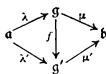
\includegraphics[keepaspectratio]{images/part001_2862d8fe.jpg}}

是交换的（即满足 \(f \circ \lambda = \lambda', \mu' \circ f = \mu\)），则称这两个扩张等价。我们说明这样的同态必为双射。首先 \(f\) 是单射。若 \(x \in \mathfrak{g}\) 满足 \(f(x) = 0\)，则 \(\mu(x) = \mu'(f(x)) = 0\)，从而 \(x = \lambda(y)\)，其中某个 \(y \in \mathfrak{a}\)；于是 \(\lambda'(y) = f(\lambda(y)) = f(x) = 0\)，故 \(y = 0\)，进而 \(x = 0\)。另一方面，\(f\) 是满射。因为 \(\mu' \circ f = \mu\) 是满射，所以 \(f(\mathfrak{g}) + \lambda'(\mathfrak{a}) = \mathfrak{g}'\)；另一方面 \(f(\mathfrak{g}) \supset f(\lambda(\mathfrak{a})) = \lambda'( \mathfrak{a})\)。

由此可知，刚才定义的两个由 a 扩张 b 之间的关系是等价关系。

命题 6. 设

\[
a \xrightarrow {\lambda} g \xrightarrow {\mu} b
\]

是由 a 扩张 b 的扩张，n 是其核。

\begin{enumerate}
\def\labelenumi{(\alph{enumi})}
\item
  若 g 有一个在 g 中补 n 的子代数 m，则 μ 在 m 上的限制是从 m 到 b 的同构。若 v 表示此限制的逆同构，则 v 是从 b 到 g 的同态，且 μ ∘ v 是 b 的恒等自同构。
\item
  反之，若存在一个同态 \(v\)，它从 \(\mathfrak{b}\) 到 \(\mathfrak{g}\)，使 \(\mu \circ v\) 是 \(\mathfrak{b}\) 的恒等自同构，则 \(v(\mathfrak{b})\) 是 \(\mathfrak{n}\) 在 \(\mathfrak{g}\) 中的补子代数。
\end{enumerate}

（a）的断言是直接的。另一方面，设 v 是从 b 到 g 的同态，且 \(\mu \circ v\) 是 b 的恒等自同构。则 \(v(b)\) 是 g 的子代数，并且 g 是 \(v(b)\) 与 \(\mu^{-1}(0) = n\) 的直和（Algebra, Chapter VIII, §1, no. 1）。

定义 6. 设

\[
a \xrightarrow {\lambda} g \xrightarrow {\mu} b
\]

是一个 \(\mathfrak{b}\) 的 \(\mathfrak{a}\)-扩张，\(\mathfrak{n}\) 是其核。如果 \(\mathfrak{g}\) 中存在一个子代数（分别为理想）补 \(\mathfrak{n}\) 于 \(\mathfrak{g}\)，则称此扩张为非本质的（分别为平凡的）。若 \(\mathfrak{n}\) 包含于 \(\mathfrak{g}\) 的中心，则称此扩张为中心扩张。

若扩张是平凡的，设 \(m\) 是 \(g\) 中补 \(n\) 于 \(g\) 的理想。则（参见第 1 号）\(g\) 自然地与李代数 \(m \times n\) 相同，因而也与李代数 \(a \times b\) 相同。反之，设 \(a\) 和 \(b\) 是两个李代数，则 \(a \times b\) 是 \(b\) 的 \(a\)-平凡扩张。

非本质的中心扩张是平凡的。事实上，设 \(\mathfrak{g}\) 是李代数，\(\mathfrak{n}\) 是包含于 \(\mathfrak{g}\) 中心的 \(\mathfrak{g}\) 的理想，\(\mathfrak{m}\) 是 \(\mathfrak{g}\) 中补 \(\mathfrak{n}\) 于 \(\mathfrak{g}\) 的子代数。则 \([\mathfrak{m},\mathfrak{g}] = [\mathfrak{m},\mathfrak{m}] + [\mathfrak{m},\mathfrak{n}] = [\mathfrak{m},\mathfrak{m}] \subset \mathfrak{m}\)，所以 \(\mathfrak{m}\) 是 \(\mathfrak{g}\) 的理想。

\subsection{半直积}

设 \(\mathfrak{a}\) 和 \(\mathfrak{b}\) 是 \(\mathbf{K}\) 上的两个李代数。构造 \(\mathfrak{b}\) 的所有由 \(\mathfrak{a}\) 作的扩张并不容易。但我们将相当简单地描述 \(\mathfrak{b}\) 的所有由 \(\mathfrak{a}\) 作的非本质扩张。

设 \(g\) 是 \(b\) 的 \(a\)-非本质扩张。我们把 \(a\) 与 \(g\) 的一个理想相同，把 \(b\) 与 \(g\) 中补 \(a\) 的一个子代数相同，并把模 \(g\) 与模 \(a \times b\) 相同。对所有 \(b \in b\)，令 \(\phi_b\) 为 \(a\) 上 \(ad_g b\) 的限制；它是 \(a\) 的导子，而映射 \(b \mapsto \phi_b\) 是从 \(b\) 到 \(a\) 的导子李代数的同态。另一方面，对 \(a, a'\) 中的 \(a\) 和 \(b, b'\) 中的 \(b\)，有：

\[
\begin{array}{r l} {[ (a, b), (a ^ {\prime}, b ^ {\prime}) ]} & {= [ a + b, a ^ {\prime} + b ^ {\prime} ]} \\ & {= [ a, a ^ {\prime} ] + [ a, b ^ {\prime} ] + [ b, a ^ {\prime} ] + [ b, b ^ {\prime} ]} \\ & {= ([ a, a ^ {\prime} ] + \phi_ {b} a ^ {\prime} - \phi_ {b ^ {\prime}} a, [ b, b ^ {\prime} ]).} \end{array}\tag{6}
\]

反之，设 \(\mathfrak{a}\) 和 \(\mathfrak{b}\) 是 \(\mathbf{K}\) 上的李代数，\(b \mapsto \phi_b\) 是从 \(\mathfrak{b}\) 到 \(\mathfrak{a}\) 的导子李代数的同态。在 \(\mathfrak{g}\)（K-模 \(\mathfrak{a}\) 与 \(\mathfrak{b}\) 的积）上，我们如下定义两个元素的括号：

\[
[ (a, b), (a ^ {\prime}, b ^ {\prime}) ] = ([ a, a ^ {\prime} ] + \phi_ {b} a ^ {\prime} - \phi_ {b ^ {\prime}} a, [ b, b ^ {\prime} ])
\]

对所有 \(a, a'\) 属于 \(\mathfrak{a}, b, b'\) 属于 \(\mathfrak{b}\)。立即可见，此括号是关于 \((a, b), (a', b')\) 的交错双线性函数；我们说明，对于 \((a, b), (a', b'), (a'', b'')\) 这三个 \(\mathfrak{a} \times \mathfrak{b}\) 中的元素，有：

\[
\begin{array}{r l} {[ (a, b), [ (a ^ {\prime}, b ^ {\prime}), (a ^ {\prime \prime}, b ^ {\prime \prime}) ] ] + [ (a ^ {\prime}, b ^ {\prime}), [ (a ^ {\prime \prime}, b ^ {\prime \prime}), (a, b) ] ]} & \\ {+ [ (a ^ {\prime \prime}, b ^ {\prime \prime}), [ (a, b), (a ^ {\prime}, b ^ {\prime}) ] ] = 0.} \end{array}\tag{7}
\]

由于 (7) 的左端是关于 \((a, b)\)、\((a', b')\)、\((a'', b'')\) 的交错三线性函数，只需在这组元素取下列形式之一时验证：

\[
(a, 0), (a ^ {\prime}, 0), (a ^ {\prime \prime}, 0)\tag{8}
\]

\[
(a, 0), (a ^ {\prime}, 0), (0, b ^ {\prime \prime})\tag{9}
\]

\[
(a, 0), (0, b ^ {\prime}), (0, b ^ {\prime \prime})\tag{10}
\]

\[
(0, b), (0, b ^ {\prime}), (0, b ^ {\prime \prime})\tag{11}
\]

在情形 (8) 和 (11) 中，关系 (7) 立即由 a 和 b 中的 Jacobi 恒等式得到。在情形 (9) 中，有

\[
\begin{array}{l} [ (a, 0), [ (a ^ {\prime}, 0), (0, b ^ {\prime \prime}) ] ] = [ (a, 0), (- \phi_ {b ^ {\prime \prime}} a ^ {\prime}, 0) ] = (- [ a, \phi_ {b ^ {\prime \prime}} a ^ {\prime} ], 0) \\ {} [ (a ^ {\prime}, 0), [ (0, b ^ {\prime \prime}), (a, 0) ] ] = [ (a ^ {\prime}, 0), (\phi_ {b ^ {\prime \prime}} a, 0) ] = ([ a ^ {\prime}, \phi_ {b ^ {\prime \prime}} a ], 0) \\ {} [ (0, b ^ {\prime \prime}), [ (a, 0), (a ^ {\prime}, 0) ] ] = [ (0, b ^ {\prime \prime}), ([ a, a ^ {\prime} ], 0) ] = (\phi_ {b ^ {\prime \prime}} ([ a, a ^ {\prime} ]), 0) \end{array}
\]

关系 (7) 由下式得到：

\[
\phi_ {b ^ {\prime \prime}} ([ a, a ^ {\prime} ]) = [ \phi_ {b ^ {\prime \prime}} a, a ^ {\prime} ] + [ a, \phi_ {b ^ {\prime \prime}} a ^ {\prime} ].
\]

在情形 (10) 中，有：

\[
[ (a, 0), [ (0, b ^ {\prime}), (0, b ^ {\prime \prime}) ] ] = [ (a, 0), (0, [ b ^ {\prime}, b ^ {\prime \prime} ]) ] = (- \phi_ {[ b ^ {\prime}, b ^ {\prime \prime} ]} a, 0)
\]

\[
[ (0, b ^ {\prime}), [ (0, b ^ {\prime \prime}), (a, 0) ] ] = [ (0, b ^ {\prime}), (\phi_ {b ^ {\prime \prime}} a, 0) ] = (\phi_ {b ^ {\prime}} \phi_ {b ^ {\prime \prime}} a, 0)
\]

\[
[ (0, b ^ {\prime \prime}), [ (a, 0), (0, b ^ {\prime}) ] ] = [ (0, b ^ {\prime \prime}), (- \phi_ {b ^ {\prime}} a, 0) ] = (- \phi_ {b ^ {\prime \prime}} \phi_ {b ^ {\prime}} a, 0)
\]

关系 (7) 由下式得到：

\[
\phi_ {[ b ^ {\prime}, b ^ {\prime \prime} ]} = \phi_ {b ^ {\prime}} \phi_ {b ^ {\prime \prime}} - \phi_ {b ^ {\prime \prime}} \phi_ {b ^ {\prime}}.
\]

于是，g 上定义了李代数结构。从 g 到 b 的映射 \((a, b) \mapsto b\) 是同态 \(\mu\)，其核 n 是 g 中形如 \((a, 0)\) 的元素组成的理想。映射 \(a \mapsto (a, 0)\) 是将 a 同构到 n 上的同构 \(\lambda\)。因此：

\[
a \xrightarrow {\lambda} g \xrightarrow {\mu} b\tag{12}
\]

这是一个核为 n 的由 a 扩张 b 的扩张，称为由 a、b、\(\phi\) 典范定义的扩张。映射 \(b \mapsto (0, b)\) 是将 b 同构到 g 的一个补 n 的子代数上的同构 v；因此该扩张是非本质的。

若在识别 \(a\) 与 \(n\) 时使用 \(\lambda\)，并在识别 \(b\) 与 \(v(b)\) 时使用 \(v\)，则对 \(a \in a\) 和 \(b \in b\)：

\[
(\mathrm{ad} b). a = [ (0, b), (a, 0) ] = (\phi_ {b} a, 0) = \phi_ {b} a.
\]

当 \(\phi = 0\) 时，\(\mathfrak{g}\) 是 \(\mathfrak{b}\) 与 \(\mathfrak{a}\) 的积李代数。一般情形下，\(\mathfrak{g}\) 称为 \(\mathfrak{b}\) 由 \(\mathfrak{a}\) 作的半直积（对应于 \(b \mapsto \phi_b\) 从 \(\mathfrak{b}\) 到 \(\mathfrak{a}\) 的导子李代数的同态）。

因此我们得到了下述命题：

命题 7. 设 a 和 b 是 K 上的两个李代数，

\[
a \xrightarrow {\lambda} g \xrightarrow {\mu} b
\]

是由 a 扩张 b 的非本质扩张，v 是将 b 同构到 g 的一个子代数上的同构，且 \(\mu \circ v\) 是 b 的恒等自同构；\(\phi\) 是相应的从 b 到 a 的导子李代数的同态。设

\[
a \xrightarrow {\lambda_ {0}} g _ {0} \xrightarrow {\mu_ {0}} b
\]

是由 a 扩张的 \(\mathfrak{b}\)、由 \(\phi\) 典范定义的非本质扩张。则映射 \((a, b) \mapsto \lambda(a) + v(b)\) 是同构 \(f\)，从 \(\mathfrak{g}_0\) 到 \(\mathfrak{g}\)，且下图

\pandocbounded{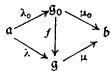
\includegraphics[keepaspectratio]{images/part001_108a7b03.jpg}}

是交换的，因此两个扩张等价。

例 1. 设 g 是 K 上的李代数，D 是 g 的导子。令 h 为交换李代数 K。映射 \(\lambda \mapsto \lambda D (\lambda \in \mathbf{K})\) 是从 h 到 g 的导子李代数的同态。我们构造 h 由 g 作的相应半直积 t。令 \(x_0\) 为 t 的元素 (0, 1)。对所有 \(x \in g\)，有 Dx = [x₀, x]。

例 2. 设 g 是 K 上的李代数，M 是 K-模，\(\rho\) 是从 g 到 gl(M) 的同态。若把 M 视为交换李代数，则 M 的导子李代数就是 gl(M)。因此，我们可以构造对应于 \(\rho\) 的 M 由 g 作的半直积 h。

特别地，令 \(\mathfrak{g} = \mathfrak{gl}(\mathbf{M})\)，\(\rho\) 为 \(\mathfrak{gl}(\mathbf{M})\) 的恒等映射。于是，\(\mathfrak{g}\) 由 \(\mathbf{M}\) 作的半直积记作 \(\mathfrak{af}(\mathbf{M})\)（或记作 \(\mathfrak{af}(n,\mathbf{K})\)，当 \(\mathbf{M} = \mathbf{K}^{n}\) 时）。\(\mathfrak{af}(\mathbf{M})\) 的元素是有序对 \((m,u)\)，其中 \(m\in \mathbf{M}\)、\(u\in \mathfrak{gl}(\mathbf{M})\)；括号定义为

\[
[ (m, u), (m ^ {\prime}, u ^ {\prime}) ] = (u (m ^ {\prime}) - u ^ {\prime} (m), [ u, u ^ {\prime} ]).
\]

*当 M 是 R 上的有限维向量空间时，\(\mathfrak{af}(M)\) 自然地与 M 的仿射群的李代数相同。*

设 \(t\) 是 \(K\) 上的李代数。线性映射 \(\theta\) 从 \(t\) 到 \(\mathfrak{af}(M)\) 可写成 \(x \mapsto ((\zeta(x), \eta(x))\)，其中 \(\zeta\) 是从 \(t\) 到 \(M\) 的线性映射，\(\eta\) 是从 \(t\) 到 \(\mathfrak{gl}(M)\) 的线性映射。我们考察 \(\zeta\) 和 \(\eta\) 为使 \(\theta\) 成为同态必须满足的条件。对 \(x \in t, y \in t\)，必须有

\[
\theta ([ x, y ]) = [ \theta (x), \theta (y) ]
\]

即

\[
\begin{array}{r l} (\zeta ([ x, y ]), \eta ([ x, y ])) & = [ (\zeta (x), \eta (x)), (\zeta (y), \eta (y)) ] \\ & = (\eta (x). \zeta (y) - \eta (y). \zeta (x), [ \eta (x), \eta (y) ]). \end{array}
\]

因此，\(\theta\) 是从 \(t\) 到 \(\mathfrak{af}(M)\) 的同态的充要条件是：\(\eta\) 是从 \(t\) 到 \(\mathfrak{gl}(M)\) 的同态，且 \(\zeta\) 满足关系式：

\[
\zeta ([ x, y ]) = \eta (x). \zeta (y) - \eta (y). \zeta (x).\tag{13}
\]

令 \(\mathbf{N}\) 为 \(\mathbf{K}\)-模 \(\mathbf{M} \times \mathbf{K}\)。取 \(t\) 为 \(\mathfrak{gl}(\mathbf{N})\) 的子代数，由 \(w \in \mathfrak{gl}(\mathbf{N})\) 且满足 \(w(\mathbf{N}) \subset \mathbf{M}\) 的元素组成。对所有 \(w \in t\)，令 \(\eta(w) \in \mathfrak{gl}(\mathbf{M})\) 为 \(w\) 在 \(\mathbf{M}\) 上的限制，并令 \(\zeta(w) = w(0,1) \in \mathbf{M}\)。对 \(w_1 \in t, w_2 \in t\)，

\[
\zeta ([ w _ {1}, w _ {2} ]) = w _ {1} (\zeta (w _ {2})) - w _ {2} (\zeta (w _ {1})) = \eta (w _ {1}). \zeta (w _ {2}) - \eta (w _ {2}). \zeta (w _ {1}).
\]

因此映射 \(w \mapsto (\zeta(w), \eta(w))\) 是同态 \(\theta\)，它从 \(t\) 到 \(\mathfrak{af}(\mathbf{M})\)。显然 \(\theta\) 是双射。令 \(\phi = \theta^{-1}\)。若 \((m, u) \in \mathfrak{af}(\mathbf{M})\)，则 \(\phi(m, u)\) 是元素 \(w\)，它是 \(t\) 中由下式定义的：

\[
w (m ^ {\prime}, \lambda) = (u (m ^ {\prime}) + \lambda m, 0).
\]

\(\mathfrak{af}(\mathbf{M})\) 常被认作子代数 \(\mathfrak{t}\)，它属于 \(\mathfrak{gl}(\mathbf{N})\)，对应的同构为 \(\phi\)。

*当 M 是 \(\mathbf{R}\) 上的有限维向量空间时，同态 \(\phi\) 从 \(\mathfrak{af}(M)\) 到 \(\mathfrak{gl}(N)\)，对应于 M 的仿射群 A 到同态 \(\psi\)，它映到 \(\mathbf{GL}(N)\)；若 \(a \in A\)，则 \(\psi(a)\) 是唯一元素 \(g\)，它属于 \(\mathbf{GL}(N)\) 且满足 \(g(m, 1) = (a(m), 1)\) 对所有 \(m \in M\) 成立。此同态是单射，而 \(\psi(A)\) 是 N 的所有平行于 M 的线性簇均保持不变的自同构组成的集合。*

\subsection{基环变换}

设 \(K_{0}\) 是含单位元的交换环，\(\rho\) 是将单位元映到单位元的从 \(K_{0}\) 到 K 的同态。设 g 是 K 上的李代数。令 \(g'\) 表示将 g 视为 \(K_{0}\) 上的代数并借助 \(\rho\) 得到的代数（参见第 1 号）。则 \(g'\) 是李代数。g 的子代数（分别为理想）是 \(g'\) 的子代数（分别为理想）。若 a 和 b 是 g 的子模，则括号 {[}a, b{]} 在 g 和 \(g'\) 中相同；因为 {[}a, b{]} 是形如

\(\sum_{i=1}^{n}\left[x_i,y_i\right]\) 的元素组成的集合，其中 \(x_{i}\in a,y_{i}\in b\)。由此 \(\mathcal{D}^p\mathfrak{g} = \mathcal{D}^p\mathfrak{g}'\)、\(\mathcal{C}^p\mathfrak{g} = \mathcal{C}^p\mathfrak{g}'\) 对所有 \(p\) 成立。

子集的中心化子在 \(\mathfrak{g}\) 和 \(\mathfrak{g}'\) 中相同。因此 \(\mathcal{C}_p\mathfrak{g} = \mathcal{C}_p\mathfrak{g}'\) 对所有 \(p\) 成立。

设 \(\mathbf{K}_1\) 是含单位元的交换环，\(\sigma\) 是将单位元映到单位元的从 \(\mathbf{K}\) 到 \(\mathbf{K}_1\) 的同态。设 \(\mathfrak{g}\) 是 \(\mathbf{K}\) 上的李代数。令 \(\mathfrak{g}_{(\mathbf{K}_1)}\) 表示 \(\mathbf{K}_1\) 上通过扩张基环由 \(\mathfrak{g}\) 导出的代数（参见第 1 号）。则 \(\mathfrak{g}_{(\mathbf{K}_1)}\) 是李代数。若 \(\mathfrak{a}\) 是 \(\mathfrak{g}\) 的子代数（分别为理想），则 \(\mathfrak{a}_{(\mathbf{K}_1)}\) 在 \(\mathfrak{g}_{(\mathbf{K}_1)}\) 中的典范像是 \(\mathfrak{g}_{(\mathbf{K}_1)}\) 的子代数（分别为理想）。若 \(\mathfrak{a}\) 和 \(\mathfrak{b}\) 是 \(\mathfrak{g}\) 的子模，则 \(\mathfrak{g}_{(\mathbf{K}_1)}\) 中 \([\mathfrak{a},\mathfrak{b}]_{(\mathbf{K}_1)}\) 的典范像，等于 \(\mathfrak{a}_{(\mathbf{K}_1)}\) 和 \(\mathfrak{b}_{(\mathbf{K}_1)}\) 的典范像的括号。由此，\(\mathcal{D}^p (\mathfrak{g}_{(\mathbf{K}_1)})\) 是 \((\mathcal{D}^p\mathfrak{g})_{(\mathbf{K}_1)}\) 的典范像，而 \(\mathcal{C}^p (\mathfrak{g}_{(\mathbf{K}_1)})\) 是 \((\mathcal{C}^p\mathfrak{g})_{(\mathbf{K}_1)}\) 的典范像。

若 K 是域，\(K_{1}\) 是 K 的扩域，\(\sigma\) 是 K 到 \(K_{1}\) 的典范嵌入，则在通常的同一视下有

\[
\begin{array}{c} [ a, b ] _ {(\mathbf {K} _ {1})} = [ a _ {(\mathbf {K} _ {1})}, b _ {(\mathbf {K} _ {1})} ], \qquad \mathcal {D} ^ {p} (\mathfrak {g} _ {(\mathbf {K} _ {1})}) = (\mathcal {D} ^ {p} \mathfrak {g}) _ {(\mathbf {K} _ {1})}, \\ \mathcal {C} ^ {p} (\mathfrak {g} _ {(\mathbf {K} _ {1})}) = (\mathcal {C} ^ {p} \mathfrak {g}) _ {(\mathbf {K} _ {1})}. \end{array}
\]

这些结果将在第 2 节第 9 号中补充完整。

若 M 是域 K 上的有限维向量空间，则 \(M_{(\mathbf{K}_{1})}\) 是 \(K_{1}\) 上的有限维向量空间，结合代数 \(\mathcal{L}(M_{(\mathbf{K}_{1})})\) 自然地与结合代数 \(\mathcal{L}(M)_{(\mathbf{K}_{1})}\) 相同。因此李代数 \(\mathfrak{gl}(M_{(\mathbf{K}_{1})})\) 自然地与李代数 \(\mathfrak{gl}(M)_{(\mathbf{K}_{1})}\) 相同。

\section{李代数的包络代数}

\subsection{包络代数的定义}

设 g 是 K 上的李代数。对于 K 上任意含单位元的结合代数 L，从 g 到 L 的 \(\alpha\)-映射是从 g 到 L 的 K-线性映射 \(\sigma\)，满足

\[
\sigma ([ x, y ]) = \sigma (x) \sigma (y) - \sigma (y) \sigma (x) \quad (x, y \text {   in   } g)
\]

（换言之，是从 \(\mathfrak{g}\) 到与 L 相关联的李代数的同态）。若 L' 是 K 上另一个含单位元的结合代数，\(\tau\) 是将 1 映到 1 的从 L 到 L' 的同态，则 \(\tau \circ \sigma\) 是一个 \(\alpha\)-映射，从 \(\mathfrak{g}\) 到 L'。我们要寻找一个含单位元的结合代数以及一个 \(\alpha\)-映射，从 \(\mathfrak{g}\) 到该代数，二者具有泛性质（Set Theory, Chapter IV, § 3, no. 1）。

定义 1. 设 \(\mathfrak{g}\) 是 \(\mathbf{K}\) 上的李代数，\(\mathbf{T}\) 是 \(\mathbf{K}\)-模 \(\mathfrak{g}\) 的张量代数，\(\mathbf{J}\) 是 \(\mathbf{T}\) 的双边理想，由张量 \(x \otimes y - y \otimes x - [x, y]\)（其中 \(x \in \mathfrak{g}, y \in \mathfrak{g}\)）生成。结合代数 \(\mathbf{U} = \mathbf{T} / \mathbf{J}\) 称为 \(\mathfrak{g}\) 的包络代数。在 \(\mathfrak{g}\) 上，将 \(\mathbf{T}\) 映到 \(\mathbf{U}\) 的典范映射的限制称为从 \(\mathfrak{g}\) 到 \(\mathbf{U}\) 的典范映射。

令 \(T_{+}\) 为 T 的双边理想，由 0 阶分量为零的张量组成。令 \(\mathrm{T}_0 = \mathrm{K}.1\) 为 T 中 0 阶元素的集合。令 \(\mathrm{U}_{+}\) 和 \(\mathrm{U}_0\) 为 \(\mathrm{T}_{+}\) 和 \(\mathrm{T}_0\) 在 U 中的典范像。由于 \(\mathrm{J} \subset \mathrm{T}_{+}\)，直和分解 \(\mathrm{T} = \mathrm{T}_0 + \mathrm{T}_{+}\) 蕴含直和分解 \(\mathrm{U} = \mathrm{U}_0 + \mathrm{U}_{+}\)。因此代数 U 有一个异于 0 的单位元，且 \(\mathrm{U}_0 = \mathrm{K}.1\)。对所有 \(x \in \mathbf{U}\)，\(x\) 在 \(\mathrm{U}_0\) 中的分量称为 \(x\) 的常数项。常数项为零的元素构成 U 的双边理想，即由 g 在 U 中的典范像生成的双边理想 \(\mathrm{U}^{+}\)。

结合代数 U 由 1 和 g 在 U 中的典范像生成。

若 \(x \in \mathfrak{g}\) 且 \(y \in \mathfrak{g}\)，则 \(x \otimes y - y \otimes x\) 与 \([x, y]\) 在 T 中模 J 同余；因此，若 \(\sigma_0\) 表示从 \(\mathfrak{g}\) 到 U 的典范映射，则

\[
\sigma_ {0} (x) \sigma_ {0} (y) - \sigma_ {0} (y) \sigma_ {0} (x) = \sigma_ {0} ([ x, y ])
\]

在 U 中成立。换言之，\(\sigma_{0}\) 是从 g 到 U 的 \(\alpha\)-映射。

命题 1. 设 \(\sigma\) 是一个 \(\alpha\)-映射，从 \(\mathfrak{g}\) 到含单位元的结合代数 \(\mathbf{L}\)。存在唯一的同态 \(\tau\)，它从 \(\mathbf{U}\) 到 \(\mathbf{L}\)，将 1 映到 1，且满足 \(\sigma = \tau \circ \sigma_0\)，其中 \(\sigma_0\) 表示从 \(\mathfrak{g}\) 到 \(\mathbf{U}\) 的典范映射。

设 \(\tau'\) 是从 T 到 L 的唯一同态，它延拓 \(\sigma\) 并将 1 映到 1。则对 g 中的 \(x, y\)，

\[
\tau^ {\prime} (x \otimes y - y \otimes x - [ x, y ]) = \sigma (x) \sigma (y) - \sigma (y) \sigma (x) - \sigma ([ x, y ]) = 0;
\]

故 \(\tau'\) 在 \(J\) 上为零，取商后定义了同态 \(\tau\)，它从 \(U\) 到 \(L\)，将 1 映到 1，并满足 \(\sigma = \tau \circ \sigma_0\)。由于 \(\tau\) 由 \(\sigma_0(g)\) 和 1 在代数 \(U\) 中生成，其唯一性是显然的。

设 \(g'\) 是 K 上的另一个李代数，U' 是其包络代数，\(\sigma_0'\) 是从 \(g'\) 到 U' 的典范映射。设 \(\phi\) 是从 g 到 g' 的同态。则 \(\sigma_0' \circ \phi\) 是从 g 到 U' 的 \(\alpha\)-映射；因此存在唯一的将 1 映到 1 的从 U 到 U' 的同态 \(\tilde{\phi}\)，使下图

\[
\begin{array}{c} g \xrightarrow {\phi} g ^ {\prime} \\ \sigma_ {0} \Biggl \downarrow \\ U \xrightarrow {\tilde {\phi}} U ^ {\prime} \end{array}
\]

是交换的。此同态将 U 中常数项为零的元素映到 U' 中常数项为零的元素。若 g'' 是 K 上的另一个李代数，\(\phi'\) 是从 g' 到 g'' 的同态，则 \(\widetilde{\phi'\circ\phi}=\widetilde{\phi}'\circ\widetilde{\phi}\)。

\subsection{李代数积的包络代数}

设 \(g_{1}, g_{2}\) 是 K 上的两个李代数，\(U_{i}\) 是 \(g_{i}\) 的包络代数，\(\sigma_{i}\) 是从 \(g_{i}\) 到 \(U_{i}\) 的典范映射（i = 1, 2）。令 \(g = g_{1} \times g_{2}\)，U 为其包络代数，\(\sigma\) 为从 g 到 U 的典范映射。\(g_{1}\) 和 \(g_{2}\) 到 g 的典范嵌入定义了从 \(U_{1}\) 和 \(U_{2}\) 到 U 的典范同态；它们的像彼此可交换，因而得到同态 \(\phi\)，它从代数 \(U_1 \otimes_K U_2\) 到代数 \(U\)，并将 1 映到 1。

命题 2. 同态 \(\phi\) 是代数同构

映射 \(\sigma': (x_1, x_2) \mapsto \sigma_1(x_1) \otimes 1 + 1 \otimes \sigma_2(x_2) (x_1 \in \mathfrak{g}_1, x_2 \in \mathfrak{g}_2)\) 是一个 \(\alpha\)-映射，从 \(\mathfrak{g}\) 到 \(\mathrm{U}_1 \otimes_{\mathbb{K}} \mathrm{U}_2\)，因此存在唯一的同态 \(\tau\)，它从 \(\mathrm{U}\) 到 \(\mathrm{U}_1 \otimes_{\mathbb{K}} \mathrm{U}_2\)，将 1 映到 1（第 1 号，命题 1），使得：

\[
\sigma^ {\prime} = \tau \circ \sigma .\tag{1}
\]

现在 \(\phi \circ \tau \circ \sigma = \phi \circ \sigma' = \sigma\)，且 \(\tau \circ \phi \circ \sigma' = \tau \circ \sigma = \sigma'\)，所以 \(\phi \circ \tau\) 和 \(\tau \circ \phi\) 分别是 U 与 \(U_1 \otimes_K U_2\) 的恒等映射。故命题得证。

\(U_{1} \otimes_{K} U_{2}\) 在同构 \(\phi\) 下与 U 相同。于是 g 到 U 的典范映射由 (1) 与下列映射相同：

\[
(x _ {1}, x _ {2}) \mapsto \sigma_ {1} (x _ {1}) \otimes 1 + 1 \otimes \sigma_ {2} (x _ {2}).
\]

类似地，若 \(g_{1},\ldots,g_{n}\) 是 K 上的李代数，其包络代数为 \(U_{1},\ldots,U_{n}\)，则 \(g_{1}\times\cdots\times g_{n}\) 的包络代数 U 自然地与 \(U_{1}\otimes_{K}\cdots\otimes_{K}U_{n}\) 相同，而 \(g_{1}\times\cdots\times g_{n}\) 到 U 的典范映射与下列映射相同：

\[
(x _ {1}, \dots , x _ {n}) \mapsto \sigma_ {1} (x _ {1}) \otimes 1 \otimes \dots \otimes 1 + \dots + 1 \otimes \dots \otimes 1 \otimes \sigma_ {n} (x _ {n})
\]

（\((\sigma_{i} \text{ 所表示的典范映射从 } g_{i} \text{ 到 } U_{i})\)）。

\subsection{李子代数的包络代数}

设 g 是 K 上的李代数，h 是 g 的子代数，\(\sigma\)、\(\sigma'\) 分别是 g、h 到其包络代数 U、V 的典范映射。于是 h 到 g 的典范嵌入 i 定义了一个从 V 到 U 的同态 i，称为典范同态，并满足 \(\sigma \circ i = i \circ \sigma'\)。代数 \(i(\mathrm{V})\) 由 1 和 \(\sigma(\mathfrak{h})\) 生成。我们将看到（第 7 号，定理 5 的推论），在重要的情形中 i 是单射。

若 \(\mathfrak{h}\) 是 \(\mathfrak{g}\) 的理想，则由 \(\sigma(\mathfrak{h})\) 生成的 U 的左理想与由 \(\sigma(\mathfrak{h})\) 生成的右理想相同，换言之，它是双边理想 R。这是因为对 \(x \in \mathfrak{h}\) 和 \(x' \in \mathfrak{g}\)，

\[
\sigma (x) \sigma (x ^ {\prime}) = \sigma (x ^ {\prime}) \sigma (x) + \sigma ([ x, x ^ {\prime} ])
\]

且 \([x, x'] \in \mathfrak{h}\)。

命题 3. 设 \(\mathfrak{h}\) 是一个理想，并令 \(\mathfrak{g}, p\) 分别表示一个李代数及其典范满同态；该同态从 \(\mathfrak{g}\) 到 \(\mathfrak{g} / \mathfrak{h}\)，W 是 \(\mathfrak{g} / \mathfrak{h}\) 的包络代数。同态：

\[
\tilde {p}: \mathrm{U} \rightarrow \mathrm{W}
\]

由 \(p\) 典范定义的映射是满射，其核是理想 \(R\)，位于 \(U\) 中，并由 \(\sigma(h)\) 生成。

令 \(\sigma''\) 为从 \(g/h\) 到 W 的典范映射。交换图：

\pandocbounded{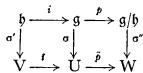
\includegraphics[keepaspectratio]{images/part001_4ab4ddcc.jpg}}

表明 \(\tilde{p}\) 在 \(\sigma(\mathfrak{h})\) 上为零，从而在 R 上为零。令 \(\psi\) 为从 U 到 U/R 的典范满同态。存在从 U/R 到 W 的同态 \(\phi\)

\pandocbounded{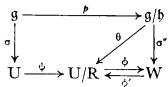
\includegraphics[keepaspectratio]{images/part001_c6a5c19d.jpg}}

到 W，使 \(\tilde{p} = \phi \circ \psi\)。映射 \(\psi \circ \sigma\) 把 \(g\) 映到 U/R，是一个 \(\alpha\)-映射，并且在 \(h\) 上为零，因而定义了一个 \(\alpha\)-映射 \(\theta\)，从 \(g / h\) 到 U/R，满足 \(\theta \circ p = \psi \circ \sigma\)。于是 \(\phi \circ \theta \circ p = \phi \circ \psi \circ \sigma = \sigma'' \circ p\)，所以 \(\phi \circ \theta = \sigma''\)。存在唯一的将 1 映到 1 的从 W 到 U/R 的同态 \(\phi'\)（第 1 号，命题 1），使 \(\theta = \phi' \circ \sigma''\)。于是 \(\phi' \circ \phi \circ \theta = \phi' \circ \sigma'' = \theta\)，且 \(\phi \circ \phi' \circ \sigma'' = \phi \circ \theta = \sigma''\)，因此 \(\phi' \circ \phi\) 和 \(\phi \circ \phi'\) 分别是 U/R 和 W 的恒等映射。证毕。

U/R 在同构 \(\phi\) 下与 W 相同。于是典范映射 \(\sigma''\) 将 \(g/h\) 映到 W，并与 \(\theta\) 相同，也就是与由取商后得到的将 \(g/h\) 映到 U/R 的映射 \(\sigma\) 相同。

\subsection{逆李代数的包络代数}

设 \(g\) 是 \(K\) 上的李代数，\(g^0\) 是逆李代数，\(\sigma\) 和 \(\sigma_0\) 分别是将 \(g\) 和 \(g^0\) 映到其包络代数 \(U\) 和 \(V\) 的典范映射。则 \(\sigma\) 是一个 \(\alpha\)-映射，从 \(g^0\) 到结合代数 \(U^0\)，即结合代数 \(U\) 的逆代数。因此存在唯一的同态 \(\phi\)，它从 \(V\) 到 \(U^0\)，将 1 映到 1，并满足 \(\sigma = \phi \circ \sigma_0\)。

命题 4. 同态 \(\phi\) 是从 \(V\) 到 \(U^0\) 的同构。

存在同态 \(\phi'\)，它将 U 映到 \(V^0\)，将 1 映到 1，并满足 \(\sigma_0 = \phi' \circ \sigma\)。可将 \(\phi'\) 视为从 \(U^0\) 到 V 的同态。于是 \(\sigma_0 = \phi' \circ \phi \circ \sigma_0\)，且 \(\sigma = \phi \circ \phi' \circ \sigma\)，从而 \(\phi' \circ \phi\) 和 \(\phi \circ \phi'\) 分别是 V 和 U 的恒等映射。故命题得证。

V 与 \(U^{0}\) 相同，这一识别由同构 \(\phi\) 给出。于是 \(\sigma_{0}\) 与 \(\sigma\) 相同。

在此同一视下，同构 \(\theta: x \mapsto -x\) 从 \(\mathfrak{g}\) 到 \(\mathfrak{g}^0\)，定义了同构 \(\tilde{\theta}\) 从 U 到 V = U \(^0\)。此同构可视为 U 的反自同构，称为 U 的主反自同构。若 \(x_{1}, \ldots, x_{n}\) 属于 \(\mathfrak{g}\)，则：

\[
\begin{array}{r l} \tilde {\theta} (\sigma (x _ {1}) \dots \sigma (x _ {n})) & = \tilde {\theta} (\sigma (x _ {n})) \dots \tilde {\theta} (\sigma (x _ {1})) = (- \sigma (x _ {n})) \dots (- \sigma (x _ {1})) \\ & = (- 1) ^ {n} \sigma (x _ {n}) \dots \sigma (x _ {1}). \end{array}\tag{2}
\]

\subsection{模的对称代数}

设 V 是 K-模。V 可唯一地视为交换李代数。于是 V 的包络代数可如下得到：令 T 为 V 的张量代数；令 I 为由张量 \(x \otimes y - y \otimes x\)（\(x \in V, y \in V\)）生成的 T 的双边理想；然后构造代数 S = T/I。

回顾 S 被称为 V 的对称代数（Algebra, Chapter III, § 6），我们简要总结本章所需的性质，其证明都是直接的。令 \(T^{n}\) 为 T 中 n 阶齐次张量的集合。则 \(\mathrm{I} = (\mathrm{I} \cap \mathrm{T}^{2}) + (\mathrm{I} \cap \mathrm{T}^{3}) + \cdots\)，从而 S 是各 \(S^{n}\)（它们是 \(T^{n}\) 的典范像）的直和。\(S^{n}\) 的元素称为 n 次齐次元素。\(S^{0} = K.1\)，\(S^{1}\) 与 V 相同，且 \(S^{n}S^{p} \subset S^{n+p}\)。代数 S 由 1 和 \(S^{1} = V\) 生成。显然 \(S^{1}\) 中任意两个元素都可交换，因而 S 是交换的。若 V 是以 \((x_{\lambda})_{\lambda \in \Lambda}\) 为基的自由 K-模，则从多项式代数 \(K[X_{\lambda}]_{\lambda \in \Lambda}\) 到 S 的典范满同态 f（将 1 映到 1，并将 \(X_{\lambda}\) 映到 \(x_{\lambda}\)，对所有 \(\lambda \in \Lambda\)）是同构：因为由 S 的泛性质（第 1 号，命题 1），存在从 S 到 \(K[X_{\lambda}]_{\lambda \in \Lambda}\) 的同态 g，将 1 映到 1，并将 \(x_{\lambda}\) 映到 \(X_{\lambda}\)，对所有 \(\lambda \in \Lambda\)，且 f 与 g 互为逆同态。

令 \(S'^{n} \subset T^n\) 为阶数 \(n\) 的齐次对称张量的集合（Algebra, Chapter III, § 5, no. 1, Definition 2）。若 \(K\) 是特征为 0 的域，则 \(S'^{n}\) 与 \(I \cap T^n\) 在 \(T^n\) 中互为补空间。事实上，设 \((x_{\lambda})_{\lambda \in \Lambda}\) 是 \(V\) 的一个基。给 \(\Lambda\) 赋予全序（Set Theory, Chapter III, § 2, no. 3, Theorem 1）。令 \(\Lambda_n\) 为由 \(n\) 个 \(\Lambda\) 中元素组成的递增序列的集合。对 \(M = (\lambda_1, \ldots, \lambda_n) \in \Lambda_n\)，令

\[
y _ {\mathrm{M}} = \frac {1}{n !} \sum_ {\sigma \in \mathfrak {S} _ {n}} x _ {\lambda_ {\sigma (1)}} \otimes \dots \otimes x _ {\lambda_ {\sigma (n)}}.
\]

\(y_{\mathbf{M}}\) 对于 \(\mathbf{M} \in \Lambda_n\) 构成向量 K-空间 \(\mathbf{S}'^n\) 的一组生成元。根据上段，它们在 \(\mathbf{S}^n\) 中的典范像构成 \(\mathbf{S}^n\) 的一个基。因此 \((y_{\mathbf{M}})_{\mathbf{M} \in \Lambda_n}\) 是 \(\mathbf{I} \cap \mathbf{T}^n\) 在 \(\mathbf{T}^n\) 中的一个补子空间的基（Algebra, Chapter II, § 1, no. 6, Proposition 4），这就证明了断言。

因此，当 K 是特征为 0 的域时，\(S'^{n}\) 上的典范映射 \(T^{n} \rightarrow S^{n}\) 的限制是从空间 \(S'^{n}\) 到空间 \(S^{n}\) 的同构，因而有逆同构。对每个 n 得到的这些逆同构定义了从空间 S 到对称张量空间 \(S' = \sum_{n \geqslant 0} S'^{n}\) 的典范同构。

\subsection{包络代数的滤子}

设 g 是 K 上的李代数，T 是 K-模 g 的张量代数。令 \(T^{n}\) 为 T 中由 n 阶齐次张量组成的子模

并令 \(\mathrm{T_n} = \sum_{i\leqslant n}\mathrm{T^i}\)。则 \(\mathrm{T_n}\subset \mathrm{T}_{n + 1},\mathrm{T_0} = \mathrm{K}.1,\mathrm{T}_{-1} = \{0\}\)，且 \(\mathrm{T_nT_p}\subset \mathrm{T}_{n + p}\)。令 \(\mathbf{U}_n\) 为 \(\mathbf{T}_n\) 在 g 的包络代数 U 中的典范像。则 \(\mathrm{U_n}\subset \mathrm{U}_{n + 1},\mathrm{U_0} = \mathrm{K}.1,\mathrm{U}_{-1} = \{0\}\)，且 \(\mathrm{U_nU_p}\subset \mathrm{U}_{n + p}\)；因此 U 可描述为由 \(\mathbf{U}_n\) 滤过的代数（Commutative Algebra, Chapter III, §2, no. I）；\(\mathrm{U_n}\) 中的元素称为滤子次数 \(\leqslant n\) 的元素。

令 \(G^n\) 为 K-模 \(U_n / U_{n-1}\)，令 G 为各 \(G^n\) 的直和这个 K-模。U 上的乘法在取商后定义了从 \(G^n \times G^m\) 到 \(G^{n+m}\) 的双线性映射，因而定义了从 \(G \times G\) 到 G 的双线性映射，该映射是结合的。于是 G 具有结合 K-代数结构。并且 \(G^n G^m \subset G^{n+m}\)。\(G^n\) 的元素称为 n 次元素。如此得到的分次代数正是滤过代数 U 的关联分次代数（Commutative Algebra, Chapter III, § 2, no. 3）。

令 \(\phi_{n}\) 为下列典范 K-线性映射的复合

\[
\mathrm{T} ^ {n} \rightarrow \mathrm{U} _ {n} \rightarrow \mathrm{G} ^ {n}.
\]

由于 \(\mathbf{T}^n\) 是 \(\mathbf{T}_{n - 1}\) 在 \(\mathbf{T}_n\) 中的补空间，\(\phi_n\) 是满射。各 \(\phi_n\) 定义了 K-线性满射 \(\phi\)，它从 \(\sum_{n}\mathbf{T}^{n} = \mathbf{T}\) 到 \(\sum_{n}\mathbf{G}^{n} = \mathbf{G}\)。

命题 5. 从 T 到 G 的映射 \(\phi\) 是将 1 映到 1 的代数同态，并且在由张量 \(x \otimes y - y \otimes x\)（\(x \in \mathfrak{g}, y \in \mathfrak{g}\)）生成的双边理想上为零。

若 \(t \in \mathbf{T}^n\) 且 \(t' \in \mathbf{T}^p\)，则按乘法定义，有 \(\phi(t)\phi(t') = \phi(tt')\)，其中乘法定义在 \(\mathbf{G}\) 上。所以 \(\phi\) 是代数同态，且显然 \(\phi(1) = 1\)。若 \(x, y\) 属于 \(\mathfrak{g}\)，则 \(x \otimes y - y \otimes x \in \mathbf{T}^2\)，且此元素在 \(\mathrm{U}_2\) 中的典范像等于 \([x, y]\) 的典范像，因而属于 \(\mathrm{U}_1\)。所以 \(\phi(x \otimes y - y \otimes x) = 0\)，命题得证。

令 S 为 K-模 g 的对称代数，\(\tau\) 为从 T 到 S 的典范同态。命题 5 表明，存在唯一的将 1 映到 1 的从代数 S 到代数 G 的同态 \(\omega\)，称为典范同态，使 \(\phi = \omega \circ \tau\)。有 \(\omega(\mathrm{S}^{n}) = \phi(\mathrm{T}^{n}) = \mathrm{G}^{n}\)。令 \(\tau_{n}\) 为 \(\tau\) 在 \(T^{n}\) 上的限制，\(\omega_{n}\) 为 \(\omega\) 在 \(S^{n}\) 上的限制，\(\psi_{n}\) 为从 \(T^{n}\) 到 \(U_{n}\) 的典范映射，\(\theta_{n}\) 为从 \(U_{n}\) 到 \(G^{n}\) 的典范映射。由 \(\omega_{n}\) 的定义，下图交换：

\pandocbounded{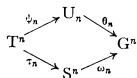
\includegraphics[keepaspectratio]{images/part001_82008693.jpg}}

命题 6. 若 K 是 Noetherian 环且 g 是有限生成模，则环 U 是左、右 Noetherian 的。

S 是 K 上的有限生成代数，因而是 Noetherian 环（Commutative Algebra, Chapter III, § 2, no. 10, Corollary 3 to Theorem 2）。所以，与 S 的商环同构的 G 是 Noetherian 的。因此 U 是左、右 Noetherian 的（Commutative Algebra, Chapter III, § 2, no. 10, Remark 2）。

推论. 设 K 是域，g 是 K 上的有限维空间。令 \(I_{1}, \ldots, I_{m}\) 为 U 中有限余维的右（分别为左）理想。则积理想 \(I_{1}I_{2}\ldots I_{m}\) 具有有限余维。

对 m 归纳，只需考虑例如两个右理想的情形。右 U-模 \(I_{1}\) 由有限个元素 \(u_{1},\ldots,u_{p}\) 生成（命题 6）。令 \(v_{1},\ldots,v_{q}\) 为 U 中的元素，使其模 \(I_{2}\) 的类生成向量空间 \(U/I_{2}\)。于是，\(I_{1}/I_{1}I_{2}\) 中 \(u_{i}v_{j}\) 的典范像生成向量空间 \(I_{1}/I_{1}I_{2}\)，该空间因而是有限维的。所以 \(\dim_{\mathbb{K}}(\mathrm{U}/\mathrm{I}_{1}\mathrm{I}_{2})=\dim_{\mathbb{K}}(\mathrm{U}/\mathrm{I}_{1})+\dim_{\mathbb{K}}(\mathrm{I}_{1}/\mathrm{I}_{1}\mathrm{I}_{2})<+\infty\)。

注. 设 \(g'\) 是环 K 上的另一个李代数，\(U'\) 是其包络代数，\(U_n'\) 是 \(U'\) 中滤子次数 \(\leqslant n\) 的元素的集合，\(U^n\)（分别为 \(U'^n\)）是 U（分别为 \(U'\)）中 g（分别为 \(g'\)）的 n 阶齐次对称张量的典范像的集合。令 \(\eta\) 为从 g 到 \(g'\) 的同态，\(\tilde{\eta}\) 为相应的从 U 到 \(U'\) 的同态。则

\[
\tilde {\eta} (\mathrm{U} _ {n}) \subset \mathrm{U} _ {n} ^ {\prime}, \quad \tilde {\eta} (\mathrm{U} ^ {n}) \subset \mathrm{U} ^ {\prime n}.
\]

特别地，U 的主反自同构保持 \(U_{n}\) 和 \(U^{n}\) 稳定。将 \(T^{n}\) 映到自身的 K-线性映射为：

\[
x _ {1} \otimes x _ {2} \otimes \dots \otimes x _ {n} \quad \text { to } \quad x _ {n} \otimes x _ {n - 1} \otimes \dots \otimes x _ {1}
\]

对 g 中所有 \(x_{1},\ldots,x_{n}\) 的映射是一个对称算子，因而保持 n 阶齐次对称张量不变。因此，U 的主反自同构在每个 \(U^{n}\) 上诱导出比为 \((-1)^{n}\) 的伸缩变换。

\subsection{Poincaré-Birkhoff-Witt 定理}

定理 1. 设 \(\mathfrak{g}\) 是李 K-代数，\(U\) 是其包络代数，G 是滤过代数 U 的关联分次代数，S 是 K-模 \(\mathfrak{g}\) 的对称代数。若 \(\mathfrak{g}\) 是自由 K-模，则典范同态 \(\omega: \mathrm{S} \to \mathrm{G}\) 是同构。

令 \((x_{\lambda})_{\lambda \in \Lambda}\) 为 K-模 g 的一个基；给 \(\Lambda\) 赋予全序（Set Theory, Chapter III, § 2, no. 3, Theorem 1）。令 P 为多项式代数 \(\mathrm{K}[z_{\lambda}]_{\lambda \in \Lambda}\)，其不定元 \(z_{\lambda}\) 与 \(x_{\lambda}\) 一一对应。对于 \(\mathrm{M} = (\lambda_1, \lambda_2, \ldots, \lambda_n)\) 中元素组成的每个序列 \(\Lambda\)，令 \(z_{\mathrm{M}}\) 表示单项式 \(z_{\lambda_1}z_{\lambda_2}\ldots z_{\lambda_n}\)，令 \(x_{\mathrm{M}}\) 表示张量 \(x_{\lambda_1}\otimes x_{\lambda_2}\otimes \dots \otimes x_{\lambda_n}\)。

当  递增时，\(z_{\mathbb{M}}\) 构成 K-模 \(\mathbf{M}\)\(\mathbf{P}\) 的一个基（约定 \(\varnothing\) 是递增序列，且 \(z_{\varnothing} = 1\)）。令 \(\mathbf{P}_p\) 为次数 \(\leqslant p\) 的多项式组成的子模。我们先证明若干引理。（为简便起见，若对序列 M 的每个指标  都有 ，就写作 \(\lambda \leqslant M\)\(\lambda \leqslant \mu\)\(\mu\)。）

引理 1. 对每个整数 \(p \geqslant 0\)，存在唯一的从 K-模 \(f_p\)\(\mathfrak{g} \otimes_{\mathbb{K}} \mathrm{P}_p\) 到 K-模 \(\mathrm{P}\) 的同态 ，满足下列条件：

\[
\left(\mathrm{A} _ {p}\right) \quad f _ {p} \left(x _ {\lambda} \otimes z _ {\mathrm{M}}\right) = z _ {\lambda} z _ {\mathrm{M}} \quad \text {   for   } \lambda \leqslant \mathrm{M}, z _ {\mathrm{M}} \in \mathrm{P} _ {p};
\]

\[
\left(\mathrm{B} _ {p}\right) \quad f _ {p} \left(x _ {\lambda} \otimes z _ {\mathrm{M}}\right) - z _ {\lambda} z _ {\mathrm{M}} \in \mathrm{P} _ {q} \quad for \quad z _ {\mathrm{M}} \in \mathrm{P} _ {q}, q \leqslant p;
\]

\[
\left(\mathrm{C} _ {p}\right) \quad f _ {p} \left(x _ {\lambda} \otimes f _ {p} \left(x _ {\mu} \otimes z _ {\mathrm{N}}\right)\right) = f _ {p} \left(x _ {\mu} \otimes f _ {p} \left(x _ {\lambda} \otimes z _ {\mathrm{N}}\right)\right) + f _ {p} \left(\left[ x _ {\lambda}, x _ {\mu} \right] \otimes z _ {\mathrm{N}}\right)
\]

对 \(z_{\mathbf{N}} \in \mathbf{P}_{p-1}\) 成立。（\((\mathbf{C}_p)\) 中出现的各项由 \((\mathbf{B}_p)\) 可知有意义。）

此外，\(f_{p}\) 在 \(\mathfrak{g} \otimes \mathrm{P}_{p-1}\) 上的限制与 \(f_{p-1}\) 一致。

最后一个断言由其余断言推出，因为 \(f_{p}\) 在 \(\mathfrak{g} \otimes_{\mathbb{K}} \mathrm{P}_{p-1}\) 上的限制满足条件 \((\mathrm{A}_{p-1})\)、\((\mathrm{B}_{p-1})\) 和 \((\mathrm{C}_{p-1})\)。我们对 p 归纳证明 \(f_{p}\) 的存在性和唯一性。当 \(p\)\(p = 0\) 时，条件 \((\mathrm{A}_0)\) 给出 \(f_0(x_\lambda \otimes 1) = z_\lambda\)，此时条件 \((\mathrm{B}_0)\) 和 \((\mathrm{C}_0)\) 显然满足。现在假设 \(f_{p-1}\) 的存在性和唯一性已经证明。我们说明，\(f_{p-1}\) 有唯一延拓 \(f_{p}\) 到 \(\mathfrak{g} \otimes_{\mathbb{K}} \mathrm{P}_{p}\)，并满足条件 \((\mathrm{A}_{p})\)、\((\mathrm{B}_{p})\) 和 \((\mathrm{C}_{p})\)。

对于含 p 个元素的递增序列 M，我们必须定义 \(f_{p}(x_{\lambda} \otimes z_{\mathbb{M}})\)。

若 \(\lambda \leqslant M\)，其值由条件 \((A_p)\) 给出。否则，M 可唯一写成 \(M\)\((\mu, N)\) 的形式，其中 \(\mu < \lambda\)、\(\mu \leqslant N\)。于是

\[
z _ {\mathrm{M}} = z _ {\mu} z _ {\mathrm{N}} = f _ {p - 1} (x _ {\mu} \otimes z _ {\mathrm{N}})
\]

由 \((\mathrm{A}_{p - 1})\)，所以 \((\mathrm{C}_p)\) 的左端就是 \(f_{p}(x_{\lambda}\otimes z_{\mathbb{M}})\)。现在 \((\mathrm{C}_p)\) 的右端已经定义好：根据 \((\mathrm{B}_{p - 1})\)，可写为：

\[
f _ {p} (x _ {\lambda} \otimes z _ {\mathrm{N}}) = f _ {p - 1} (x _ {\lambda} \otimes z _ {\mathrm{N}}) = z _ {\lambda} z _ {\mathrm{N}} + w
\]

其中 \(w \in \mathbf{P}_{p-1}\)；因此 \((\mathbf{C}_p)\) 的右端变为：

\[
z _ {\lambda} z _ {\mu} z _ {N} + f _ {p - 1} (x _ {\mu} \otimes w) + f _ {p - 1} ([ x _ {\lambda}, x _ {\mu} ] \otimes z _ {N}).
\]

这样便唯一确定了 \(f_{p}\)，且显然满足条件 \((\mathbf{A}_{p})\) 和 \((\mathbf{B}_{p})\)。当 \((\mathbf{C}_{p})\)\(\mu < \lambda\)、\(\mu \leqslant N\) 时，条件  成立。由于 \([x_{\mu}, x_{\lambda}] = -[x_{\lambda}, x_{\mu}]\)，当 \((\mathbf{C}_{p})\)\(\lambda < \mu\)、\(\lambda \leqslant N\) 时，条件 \((\mathbf{C}_{p})\) 也成立。当 \(\lambda = \mu\) 时 \((\mathbf{C}_{p})\) 显然成立，所以只要 \(\lambda \leqslant N\) 或 \(\mu \leqslant N\)， 就成立。若这些不等式均不成立，则 \(N = (\nu, Q)\)，其中 \(\nu \leqslant Q\)、\(\nu < \lambda\)、\(\nu < \mu\)。以下简写 \(f_{p}(x \otimes z) = xz\)（其中 \(x \in g\)、\(z \in P_{p}\)），由归纳假设有：

\[
x _ {\mu} z _ {N} = x _ {\mu} (x _ {\nu} z _ {Q}) = x _ {\nu} (x _ {\mu} z _ {Q}) + [ x _ {\mu}, x _ {\nu} ] z _ {Q}.
\]

现在 \(x_{\mu}z_{\mathbf{Q}}\) 具有 \(z_{\mu}z_{\mathbf{Q}} + w\) 的形式，其中 \(w\in \mathrm{P}_{p - 2}\)。由于  且 ，可将 (C \(_{p}\) ) 应用于 \(x_{\lambda}(x_{\nu}(z_{\mu}z_{\mathbf{Q}}))\)；根据归纳假设，也可应用于 \(\nu \leqslant Q\)\(\nu < \mu\)\(x_{\lambda}(x_{\nu}w)\)，因而可应用于 \(x_{\lambda}(x_{\nu}(x_{\mu}z_{\mathbf{Q}}))\)。因此：

\[
\begin{array}{r l} x _ {\lambda} (x _ {\mu} z _ {N}) = x _ {\nu} (x _ {\lambda} (x _ {\mu} z _ {\mathbb {Q}})) & + [ x _ {\lambda}, x _ {\nu} ] (x _ {\mu} z _ {\mathbb {Q}}) + [ x _ {\mu}, x _ {\nu} ] (x _ {\lambda} z _ {\mathbb {Q}}) \\ & + [ x _ {\lambda}, [ x _ {\mu}, x _ {\nu} ] ] z _ {\mathbb {Q}}. \end{array}
\]

交换 \(\lambda\) 与 \(\mu\) 后相减：

\[
\begin{array}{r l} {x _ {\lambda} (x _ {\mu} z _ {N}) - x _ {\mu} (x _ {\lambda} z _ {N})} & {= x _ {\nu} (x _ {\lambda} (x _ {\mu} z _ {Q}) - x _ {\mu} (x _ {\lambda} z _ {Q}))} \\ & {\quad + [ x _ {\lambda}, [ x _ {\mu}, x _ {\nu} ] ] z _ {Q} - [ x _ {\mu}, [ x _ {\lambda}, x _ {\nu} ] ] z _ {Q}} \\ & {= x _ {\nu} ([ x _ {\lambda}, x _ {\mu} ] z _ {Q}) + [ x _ {\lambda}, [ x _ {\mu}, x _ {\nu} ] ] z _ {Q} + [ x _ {\mu}, [ x _ {\nu}, x _ {\lambda} ] ] z _ {Q}} \\ & {= [ x _ {\lambda}, x _ {\mu} ] (x _ {\nu} z _ {Q}) + ([ x _ {\nu}, [ x _ {\lambda}, x _ {\mu} ] ]} \\ & {\quad + [ x _ {\lambda}, [ x _ {\mu}, x _ {\nu} ] ] + [ x _ {\mu}, [ x _ {\nu}, x _ {\lambda} ] ]) z _ {Q}} \end{array}
\]

从而由 Jacobi 恒等式

\[
x _ {\lambda} (x _ {\mu} z _ {N}) - x _ {\mu} (x _ {\lambda} z _ {N}) = [ x _ {\lambda}, x _ {\mu} ] z _ {N}
\]

这就完成了引理 1 的证明。

引理 2. 存在从  到  的 \(\alpha\)-映射 \(\sigma\)\(\mathfrak{g}\)\(\mathcal{L}_{\mathbf{K}}(\mathbf{P})\)，使得：

\begin{enumerate}
\def\labelenumi{(\arabic{enumi})}
\item
  \(\sigma(x_{\lambda})z_{\mathbf{M}} = z_{\lambda}z_{\mathbf{M}}\) 对 \(\lambda \leqslant \mathbf{M}\) 成立；
\item
  \(\sigma(x_{\lambda})z_{\mathbf{M}} \equiv z_{\lambda}z_{\mathbf{M}} (\mathrm{mod.~P}_{p})\) 若 \(\mathbf{M}\) 含有 \(p\) 个元素。
\end{enumerate}

由引理 1，对所有 p，存在从 K-模  到 P 的同态 \(f\)，满足条件 \(\mathfrak{g} \otimes_{\mathbb{K}} \mathrm{P}_p\)\(p\)\((\mathrm{A}_p), (\mathrm{B}_p), (\mathrm{C}_p)\)（以 f 替代 \(f_p\)）。此同态定义了从 K-模 \(f\)\(\sigma\)\(\mathfrak{g}\) 到 K-模 \(\mathcal{L}_{\mathbb{K}}(\mathrm{P})\) 的同态 \(\sigma\)，并且由于条件 \(\alpha\)\((\mathrm{C}_p)\)，\(\sigma\) 是 -映射。最后，由于条件 \((\mathrm{A}_p)\) 和 \((\mathrm{B}_p)\)， 满足本引理的性质 (1) 和 (2)。

引理 3. 设 \(t\) 是 \(\mathrm{T}_n \cap \mathrm{J}\) 中的张量。t 的 n 阶齐次分量 \(t_n\) 属于典范同态 \(t\)\(n\)\(\mathrm{T} \to \mathrm{S}\) 的核 I。

我们将 \(t_n\) 写成 \(\sum_{i=1}^{r} x_{\mathrm{M}_i}\) 的形式，其中 \(\mathrm{M}_i\) 是由 \(n\)\(\Lambda\) 中 n 个元素组成的序列。映射 \(\sigma\) 延拓为从代数 T 到代数 \(T\)\(\mathcal{L}_K(P)\) 的同态（仍记为 \(\sigma\)），并且在 \(J\) 上为零。由引理 2，\(\sigma(t)\) . 1 是一个多项式，其最高次数的项为 \(\sum_{i=1}^{r} z_{\mathrm{M}_i}\)。由于 \(t \in J\)，\(\sigma(t) = 0\)，所以在 P 中 \(\sum_{i=1}^{r} z_{\mathrm{M}_i} = 0\)。现在，由于 g 具有基 \(P\)\(P\)\(S\)\(g\)\((x_\lambda)\)，P 自然地与 S 相同。因此 \(t_n\) 在 S 中的典范像为零，即 \(S\)\(t_n \in I\)。

现在可以证明定理 1。必须证明从 S 到 G 的典范同态是单射。换言之，若 \(t \in \mathrm{T}^n\)，\(\psi\) 表示从 T 到 U 的典范满同态，就必须证明条件 \(\psi(t) \in \mathrm{U}_{n-1}\) 蕴含 \(t \in I\)。现在，\(\psi(t) \in \mathrm{U}_{n-1}\) 意味着存在 \(t' \in \mathrm{T}_{n-1}\) 中的张量，使 \(t - t' \in J\)。张量 \(t - t'\) 以 t 作为 n 阶齐次分量，因此由引理 3 有 \(t\)\(n\)\(t \in I\)。

推论 1. 设 \(\mathfrak{g}\) 是自由 K-模。令 W 为 \(\mathbf{T}^n\) 的子 K-模。

若按图 (3) 的记号，\(\tau_{n}\) 在 W 上的限制是从 W 到 \(\mathbf{S}^n\) 的同构，则 \(\psi_{n}\) 在 W 上的限制是从 W 到  中 \(\mathbf{U}_{n-1}\)\(\mathbf{U}_n\) 的一个补空间的同构。

\(\omega_{n} \circ \tau_{n}\) 在 W 上的限制是从 W 到 \(G^{n}\) 的双射；\(\theta_{n} \circ \psi_{n}\) 在 W 上的限制也如此。故推论得证。

推论 2. 若 \(\mathfrak{g}\) 是自由 K-模，则 \(\mathfrak{g}\) 到其包络代数的典范映射是单射。

取 \(\mathbf{W} = \mathbf{T}^1\) 后由推论 1 得到。

当 g 是自由 K-模时（特别是当 K 为域时），在 g 到 U 的典范映射下，将 g 与 U 的一个子模相同。从下面的推论开始采用这一约定。

推论 3. 若 \(\mathfrak{g}\) 有一个全序基 \((x_{\lambda})_{\lambda \in \Lambda}\)，则包络代数  的元素 \(x_{\lambda_1}x_{\lambda_2}\ldots x_{\lambda_n}\)（其中 \(\mathbf{U}\)\((\lambda_1,\dots ,\lambda_n)\) 是 \(\Lambda\) 中元素组成的任意有限递增序列）构成 K-模 \(\mathbf{U}\) 的一个基。

令 \(\Lambda_{n}\) 为 \(n\)\(\Lambda\) 中 n 个元素的递增序列的集合。对 \(\mathrm{M} = (\lambda_1, \ldots, \lambda_n) \in \Lambda_n\)，令 \(y_{\mathrm{M}} = x_{\lambda_1} \otimes x_{\lambda_2} \otimes \dots \otimes x_{\lambda_n}\)。令 \(\mathrm{W}\) 为以  为基的 \(\mathrm{T}^n\) 的子模。推论 1 表明，\((y_{\mathrm{M}})_{\mathrm{M} \in \Lambda_n}\)\(\psi_n\) 在 \(\mathrm{W}\) 上的限制是从 \(\mathrm{W}\) 到  中 \(\mathrm{U}_{n-1}\)\(\mathrm{U}_n\) 的一个补空间的同构。但

\[
\psi_ {n} (y _ {\mathrm{M}}) = x _ {\lambda_ {1}} x _ {\lambda_ {2}} \dots x _ {\lambda_ {n}},
\]

由此推论得证。

推论 4. 令 \(S'^{n} \subset T^n\)\(n\)\(K\) 为 n 阶齐次对称张量的集合。设 K 是特征为 0 的域。则典范映射的复合映射

\[
\mathrm{S} ^ {n} \rightarrow \mathrm{S} ^ {\prime n} \rightarrow \mathrm{U} _ {n}
\]

是从向量空间 \(\mathbf{S}^n\) 到  中 \(\mathbf{U}_{n-1}\)\(\mathbf{U}_n\) 的一个补空间的同构。

取 \(W = S'^n\) 后由推论 1 得到。

以下设 \(\mathbf{K}\) 是特征为 0 的域。令 \(\eta_{n}\) 为刚才定义的从 \(S^n\) 到 \(U_n\) 的映射。令 \(U^n = \eta_n(S^n)\)。向量空间 U 是各 \(U\)\(U^n\) 的直和。各 \(\eta_{n}\) 定义了从向量空间 \(\eta\)\(S = \sum_{n} S^n\) 到向量空间 \(U = \sum_{n} U^n\) 的同构 \(S\)\(U\)，称为从 S 到 U 的典范同构；这不是代数同构。我们有交换图：

\pandocbounded{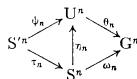
\includegraphics[keepaspectratio]{images/part001_756df219.jpg}}

其中每个箭头表示向量空间同构。若 \(x_{1}, x_{2}, \ldots, x_{n}\) 属于 \(g\)，则 \(\eta_{n}\) 将在 S 中计算的乘积 \(x_{1}x_{2}\ldots x_{n}\) 映到元素

\[
\frac {1}{n !} \sum_ {\sigma \in \mathfrak {S} _ {n}} x _ {\sigma (1)} x _ {\sigma (2)} \dots x _ {\sigma (n)}
\]

该元素在 U 中计算。

推论 5. 设 \(\mathfrak{h}\) 是李代数 \(\mathfrak{g}\) 的子代数，\(\mathrm{U}'\) 是其包络代数。假设 K-模 \(\mathfrak{h}\) 和 \(\mathfrak{g} / \mathfrak{h}\) 是自由的（例如 K 为域时）。令 \(\mathrm{K}\)\((x_{\alpha})_{\alpha \in \mathbb{L}}\) 为 \(\mathfrak{h}\) 的一个基，\((y_{\beta})_{\beta \in \mathbb{M}}\) 为 \(\mathfrak{g}\) 中的一族元素，使它们在 \(\mathfrak{g} / \mathfrak{h}\) 中的典范像构成 \(\mathfrak{g} / \mathfrak{h}\) 的一个基。

\begin{enumerate}
\def\labelenumi{(\alph{enumi})}
\item
  从 \(\mathbf{U}'\) 到 \(\mathbf{U}\) 的典范同态是单射。
\item
  若 \(\mathbf{M}\) 全序，则元素 \(y_{\beta_1} \ldots y_{\beta_q}\)（其中 \(\beta_1 \leqslant \cdots \leqslant \beta_q\)）构成把 \(\mathbf{U}\) 视为 \(\mathbf{U}'\) 的左模或右模时的一个基。
\end{enumerate}

给 \(L \cup M\) 赋予全序，使 L 中每个元素都小于 M 中每个元素。在  中计算的元素 \(x_{\alpha_{1}}x_{\alpha_{2}}\ldots x_{\alpha_{p}}\)（其中 \(U'\)\(\alpha_{1} \leqslant \cdots \leqslant \alpha_{p}\)）构成 \(U'\) 的一个基（推论 3）。元素

\[
x _ {\alpha_ {1}} \dots x _ {\alpha_ {p}} y _ {\beta_ {1}} \dots y _ {\beta_ {q}}
\]

在 U 中计算的这些元素（其中 \(\alpha_{1} \leqslant \cdots \leqslant \alpha_{p} \leqslant \beta_{1} \leqslant \cdots \leqslant \beta_{q}\)）同样构成 U 的一个基。因此，U' 到 U 的典范同态将 U' 的一个基中的元素映到 U 中线性无关的元素，因而是单射。此外可见，\(y_{\beta_1} \ldots y_{\beta_q}\)（其中 \(\beta_{1} \leqslant \cdots \leqslant \beta_{q}\)）构成把 U 视为左 U'-模时的一个基。给  排序，使 M 中每个元素都小于 L 中每个元素，同样可见，\(y_{\beta_1} \ldots y_{\beta_q}\)（其中 \(\beta_{1} \leqslant \cdots \leqslant \beta_{q}\)）构成把 U 视为右 U'-模时的一个基。

在推论 5 的条件下，通过 U' 到 U 的典范同态，将 U' 与 U 中由 h 生成的子代数相同。

推论 6. 假设 K-模 g 是子代数 \(g_{1}, g_{2}, \ldots, g_{n}\) 的直和，且每个 \(g_{i}\) 都是自由 K-模。令 \(U_{i}\) 为 \(g_{i}\) 的包络代数（\(1 \leqslant i \leqslant n\)）。令 \(\phi\) 为从 K-模 \(U_{1} \otimes_{K} \cdots \otimes_{K} U_{n}\) 到 U 的 K-线性映射，它由从  到 U 的多线性映射（\(u_{1}, \ldots, u_{n}\)）\(\mapsto u_{1} \ldots u_{n}\) 定义。则 \(U_{1} \times \cdots \times U_{n}\)\(\phi\) 是 K-模同构。

令 \((x_{\lambda}^{i})_{\lambda \in L_{i}}\) 为 \(g_{i}\) 的一个基。给 \(L_{1} \cup \cdots \cup L_{n}\) 赋予全序，使当  时 \(L_{i}\) 中每个元素都大于 \(L_{j}\)\(i \geqslant j\) 中每个元素。则元素：

\[
\left(x _ {\lambda_ {1}} ^ {1} x _ {\lambda_ {2}} ^ {1} \dots x _ {\lambda_ {p}} ^ {1}\right) \otimes \dots \otimes \left(x _ {\nu _ {1}} ^ {n} x _ {\nu _ {2}} ^ {n} \dots x _ {\nu _ {q}} ^ {n}\right),
\]

其中 \(\lambda_{1}\leqslant\lambda_{2}\leqslant\cdots\leqslant\lambda_{p}\leqslant\cdots\leqslant\nu_{1}\leqslant\nu_{2}\leqslant\cdots\leqslant\nu_{q}\)，构成 \(U_{1}\otimes_{K}\cdots\otimes_{K}U_{n}\) 的一个基。它们经 \(\phi\) 映到元素：

\[
x _ {\lambda_ {1}} ^ {1} x _ {\lambda_ {2}} ^ {1} \dots x _ {\lambda_ {p}} ^ {1} \dots x _ {\nu_ {1}} ^ {n} x _ {\nu_ {2}} ^ {n} \dots x _ {\nu_ {q}} ^ {n}
\]

这些元素构成 U 的一个基。故推论得证。

推论 7. 若 K 是整环且 g 是自由 K-模，则代数 U 没有零因子。

G 与 K 上的多项式代数同构（定理 1），因而是整环（Algebra, Chapter IV, § 1, no. 4, Theorem 1）。故推论成立（Commutative Algebra, Chapter III, § 2, no. 3, Proposition 1）。

\subsection{导子的延拓}

引理 4. 设 V 是 K-模，T 是 V 的张量代数。设 u 是 V 的自同态。存在唯一的延拓 u 的 T 的导子。此导子与 T 上的对称算子交换。

令 \(F = V \times V \times \cdots \times V\)（n 个因子）。映射

\[
\begin{array}{r l} (x _ {1}, \ldots , x _ {n}) & \mapsto u x _ {1} \otimes x _ {2} \otimes \dots \otimes x _ {n} \\ & \qquad + x _ {1} \otimes u x _ {2} \otimes \dots \otimes x _ {n} + \dots + x _ {1} \otimes x _ {2} \otimes \dots \otimes u x _ {n} \end{array}
\]

从 F 到  V 是多线性的。因此存在 \(\bigotimes^{n}\) V 的自同态 \(u_{n}\)\(\bigotimes^{n}\)，使得：

\[
u _ {n} \left(x _ {1} \otimes \dots \otimes x _ {n}\right) = u x _ {1} \otimes \dots \otimes x _ {n} + \dots + x _ {1} \otimes \dots \otimes u x _ {n}
\]

对 V 中所有 \(x_1, \ldots, x_n\) 成立。于是 \(u_1 = u\)。令 v 为 K-模 T 的自同态，它在每个 \(v\) 上与 \(u_n\) 一致，并在 \(\mathrm{T}^n = \bigotimes^n \mathrm{V}\)\(\mathrm{T}^0 = \mathrm{K}. 1\) 上为零。我们证明 v 是 T 的导子。若 \(v\)\(x_1, \ldots, x_n, y_1, \ldots, y_p\) 是 V 的元素，则

\[
\begin{array}{l} v ((x _ {1} \otimes \dots \otimes x _ {n}) \otimes (y _ {1} \otimes \dots \otimes y _ {p})) \\ = \sum_ {i = 1} ^ {n} x _ {1} \otimes \dots \otimes x _ {i - 1} \otimes u x _ {i} \otimes x _ {i + 1} \otimes \dots \otimes x _ {n} \otimes y _ {1} \otimes \dots \otimes y _ {p} \\ \qquad + \sum_ {j = 1} ^ {p} x _ {1} \otimes \dots \otimes x _ {n} \otimes y _ {1} \otimes \dots \otimes y _ {j - 1} \otimes u y _ {j} \otimes y _ {j + 1} \otimes \dots \otimes y _ {p} \\ = v (x _ {1} \otimes \dots \otimes x _ {n}) \otimes (y _ {1} \otimes \dots \otimes y _ {p}) + (x _ {1} \otimes \dots \otimes x _ {n}) \otimes v (y _ {1} \otimes \dots \otimes y _ {p}). \end{array}
\]

\(v\)\(v\)由线性性可知 v 是导子。v 的唯一性是显然的。

最后，显然 \(u_{n}\) 与 \(\otimes V\) 上的所有对称算子交换，因而得到最后一个断言。

命题 7. 设 \(\mathfrak{g}\) 是李代数，U 是其包络代数，\(\sigma\) 是从 \(\mathfrak{g}\) 到 U 的典范映射，D 是 \(\mathfrak{g}\) 的导子。

\begin{enumerate}
\def\labelenumi{(\alph{enumi})}
\item
  存在唯一的 U 的导子 \(\mathrm{D_U}\)，使 \(\sigma \circ \mathrm{D} = \mathrm{D_U} \circ \sigma\)（即当 \(\mathrm{D_U}\)\(\mathfrak{g}\) 在 \(\sigma\) 下可与 U 的一个子模相同时， 延拓 D）。
\item
  \(D_{U}\) 保持 \(U_{n}\) 以及 g 上 n 阶齐次对称张量在 U 中的像的集合 \(U^{n}\) 稳定。
\item
  \(\mathbf{D}_{\mathbf{U}}\) 与 \(\mathbf{U}\) 的主反自同构交换。
\item
  若 \(\mathbf{D}\) 是由 \(\mathfrak{g}\) 的元素 \(x\) 定义的 \(\mathfrak{g}\) 的内导子，则 \(\mathrm{D}_{\mathbf{U}}\) 是由  定义的 \(\mathbf{U}\)\(\sigma(x)\) 的内导子。
\end{enumerate}

令 \(D_T\)\(T\)\(g\)\(D\)\(J\)\(T\) 为延拓 D 的 g 的张量代数 T 的导子（引理 4）。由

\[
x \otimes y - y \otimes x - [ x, y ]
\]

生成的 T 的双边理想 J 在 \((x,y \text{ 属于 } \mathfrak{g})\)\(\mathrm{D}_{\mathrm{T}}\) 下稳定。其中：

\[
\begin{array}{r} \mathrm{D} _ {\mathrm{T}} (x \otimes y - y \otimes x - [ x, y ]) = \mathrm{D} x \otimes y - y \otimes \mathrm{D} x - [ \mathrm{D} x, y ] \\ + x \otimes \mathrm{D} y - \mathrm{D} y \otimes x - [ x, \mathrm{D} y ]. \end{array}
\]

取商后，\(D_{T}\) 定义了 U 的导子 \(D_{U}\)，满足 \(\sigma \circ D = D_{U} \circ \sigma\)。由于 1 和  生成代数 U，\(D_{U}\) 的唯一性是直接的。断言 (b) 是显然的。令 A 为 U 的主反自同构。现在证明 (c)。若 \(\sigma(\mathfrak{g})\)\(x_{1}, \ldots, x_{n}\) 属于 g，则

\[
\begin{array}{r l} \mathrm{D} _ {\mathrm{U}} \mathrm{A} (\sigma (x _ {1}) \dots \sigma (x _ {n})) & = \mathrm{D} _ {\mathrm{U}} ((- 1) ^ {n} \sigma (x _ {n}) \dots \sigma (x _ {1})) \\ & = (- 1) ^ {n} \sum_ {i = 1} ^ {n} \sigma (x _ {n}) \dots \mathrm{D} _ {\mathrm{U}} (\sigma (x _ {i})) \dots \sigma (x _ {1}) \\ & = (- 1) ^ {n} \sum_ {i = 1} ^ {n} \sigma (x _ {n}) \dots \sigma (\mathrm{D} x _ {i}) \dots \sigma (x _ {1}) \\ & = \mathrm{A} \bigg (\sum_ {i = 1} ^ {n} \sigma (x _ {1}) \dots \sigma (\mathrm{D} x _ {i}) \dots \sigma (x _ {n}) \bigg) \\ & = \mathrm{AD} _ {\mathrm{U}} (\sigma (x _ {1}) \dots \sigma (x _ {n})). \end{array}
\]

最后，设 \(x \in \mathfrak{g}\)。令 \(\Delta\) 为 U 的内导子 \(y \mapsto \sigma(x)y - y\sigma(x)\)（Algebra, Chapter IV, § 4, no. 3, Example 2）。则对 \(x' \in \mathfrak{g}\)，

\[
(\Delta \circ \sigma) (x ^ {\prime}) = \sigma (x) \sigma (x ^ {\prime}) - \sigma (x ^ {\prime}) \sigma (x) = \sigma ([ x, x ^ {\prime} ]) = (\sigma \circ \operatorname{ad} x) (x ^ {\prime}),
\]

所以 \(\Delta \circ \sigma = \sigma \circ \operatorname{ad} x\)。证明完毕。

将命题 7 应用于交换李代数的情形可见，K-模的每个自同态 u 都能唯一延拓为该模的对称代数的导子；取商后，此导子由延拓 u 的张量代数导子导出。

再次设 g 是 K 上的李代数，D 是 g 的导子。沿用前面的记号 T、S、U、G。令 \(D_{T}\)、\(D_{S}\) 为分别延拓 D 的 T、S 的导子，令 \(D_{U}\) 为满足 \(\sigma \circ D = D_{U} \circ \sigma\) 的 U 的唯一导子。由于 \(D_{U}\) 保持 \(U_{n}\) 稳定，取商后 \(D_{U}\) 定义了 G 的导子 \(D_{G}\)。由于取商时 \(D_{U}\) 和 \(D_{S}\) 都由 \(D_{T}\) 导出，图 (3) 的交换性表明，\(D_{G}\) 也可由第 6 号定义的同态  从 \(D_{S}\) 导出。若进一步 K 是特征为 0 的域，则图 (4) 的同构将 \(\omega\)\(D_{T}\)、\(D_{S}\)、\(D_{U}\)、\(D_{G}\) 在 \(S^{n}\)、\(S^{n}\)、\(U^{n}\)、\(G^{n}\) 上的限制彼此对应。因此，S 到 U 的典范同构将 \(D_{S}\) 映到 \(D_{U}\)。

\subsection{基环的扩张}

设 g 是 K 上的李代数，T 是其张量代数，J 是由 \(x \otimes y - y \otimes x - [x, y]\)（x, y 属于 g）生成的 T 的双边理想，U = T/J。设 \(K_{1}\) 是含单位元的交换环，\(\sigma\) 是将 1 映到 1 的从 K 到 \(K_{1}\) 的同态。则 \(\mathfrak{g}_{(\mathbf{K}_{1})}\) 的张量代数自然地与 \(\mathrm{T}_{(\mathbf{K}_{1})}\) 相同。令 J' 为由下式生成的 \(J'\)\(\mathrm{T}_{(\mathbf{K}_{1})}\) 的双边理想：

\[
x ^ {\prime} \otimes y ^ {\prime} - y ^ {\prime} \otimes x ^ {\prime} - [ x ^ {\prime}, y ^ {\prime} ]
\]

\((x', y' \text{ 属于 } g_{(K_1)})\)。显然，\(J_{(K_1)}\) 在 \(T_{(K_1)}\) 中的典范像包含于 J'。要看出两者相等，只需证明：若 \(J'\)\(J'\)\(x'\) 和 \(y'\) 表示 \(g_{(K_1)}\) 中的两个元素，则 \(x' \otimes y' - y' \otimes x' - [x', y']\) 属于此像。现在

\[
x ^ {\prime} = \sum_ {i} x _ {i} \otimes \lambda_ {i}, y ^ {\prime} = \sum_ {j} y _ {j} \otimes \mu_ {j} (x _ {i}, y _ {j} \text {   in   } \mathfrak {g}, \lambda_ {i}, \mu_ {j} \text {   in   } \mathrm{K} _ {1});
\]

因此

\[
x ^ {\prime} \otimes y ^ {\prime} - y ^ {\prime} \otimes x ^ {\prime} - [ x ^ {\prime}, y ^ {\prime} ] = \sum_ {i, j} (x _ {i} \otimes y _ {j} - y _ {j} \otimes x _ {i} - [ x _ {i}, y _ {j} ]) \otimes \lambda_ {i} \mu_ {j}
\]

这就证明了断言。于是可见，\(\mathrm{U}_{(\mathbf{K}_{1})} = (\mathrm{T}/\mathrm{J})_{(\mathbf{K}_{1})}\) 自然地与 \(\mathrm{T}_{(\mathbf{K}_{1})}/\mathrm{J}'\) 相同：\(\mathfrak{g}_{(\mathbf{K}_{1})}\) 的包络代数自然地与 \(\mathrm{U}_{(\mathbf{K}_{1})}\) 相同，而 \(\mathfrak{g}_{(\mathbf{K}_{1})}\) 到其包络代数的典范映射与 \(\sigma \otimes 1\) 相同（其中 \(\sigma\) 表示 g 到 U 的典范映射）。

\section{表示}


\subsection{表示}

定义 1. 设 \(\mathfrak{g}\) 是 \(\mathbf{K}\) 上的李代数，\(\mathbf{M}\) 是一个 \(\mathbf{K}\) -模。从 \(\mathfrak{g}\) 到李代数 \(\mathfrak{gl}(\mathbf{M})\) 的同态称为 \(\mathfrak{g}\) 在模 \(\mathbf{M}\) 上的表示。单射表示称为忠实表示。如果 \(\mathbf{K}\) 是域，则 \(\mathbf{M}\) 在 \(\mathbf{K}\) 上的维数（有限或无限）称为该表示的维数。\(x \mapsto \operatorname{ad} x\) 在 \(\mathfrak{g}\) -模 \(\mathbf{K}\) 上的表示 \(\mathfrak{g}\) 称为 \(\mathfrak{g}\) 的伴随表示。

因此，g 在 M 上的表示是从 g 到 M 的自同态模的 K-线性映射 \(\rho\)，满足

\[
\rho ([ x, y ]). m = \rho (x) \rho (y). m - \rho (y) \rho (x). m
\]

对所有 \(x \in g, y \in g, m \in M.\)

*例. 设 G 是实李群，g 是其李代数，\(\rho\) 是 G 在有限维实向量空间 E 上的解析表示。那么，相应的从 g 到 gl(E) 的同态就是 g 在 E 上的表示。*

设 \(\mathbf{U}\) 是 \(\mathfrak{g}\) 的包络代数。第 §2 节第 1 号的命题 1 在 \(\mathfrak{g}\) 在 \(\mathbf{M}\) 上的表示与 \(\mathbf{U}\) 在 \(\mathbf{M}\) 上的表示的集合之间建立了一一对应。另一方面，我们知道（《代数》，第 VIII 章，§13，第 1 号），结合代数 \(\mathbf{U}\) 的表示这一概念与左 \(\mathbf{U}\)-模这一概念等价。

定义 2. 设 g 是 K 上的李代数，U 是其包络代数。U 上的有单位元左模称为左 g-模，或简称 g-模。

若 M 是 g-模且 \(x \in U\)，则以 \(x_{M}\) 表示由 x 在 M 上定义的自同态（参见《代数》，第 VIII 章，§ 1，第 2 号）。

U 上的有单位元右模称为右 g-模。这样的模可与左 \(U^{0}\)-模等同，即（§2，第 4 号）可与左 \(g^{0}\)-模等同。

设 \(\phi\) 是 U 的主反自同构。如果 M 是右 g-模，则在 M 上规定左 g-模结构，写作 \(a.m = m.\phi (a)\)，其中 \(m\in \mathbf{M}\)，\(a\in \mathrm{U}\)。

模论中的概念和结果可以翻译成表示的语言：

\begin{enumerate}
\def\labelenumi{(\arabic{enumi})}
\tightlist
\item
  \(\rho\) 在 \(\rho'\) 和 \(\mathfrak{g}\) 上的两个表示 \(\mathbf{M}\) 和 \(\mathbf{M}'\)，当 \(\mathfrak{g}\)-模 \(\mathbf{M}\) 和 \(\mathbf{M}'\) 同构时，称为相似的或同构的。为此，当且仅当存在一个从 K-模 \(u\) 到 K-模 \(\mathbf{M}\) 的同构 \(\mathbf{M}'\)，使得
\end{enumerate}

\[
\rho^ {\prime} (x) = u \circ \rho (x) \circ u ^ {- 1}
\]

对所有 \(x \in g\)。

\begin{enumerate}
\def\labelenumi{(\arabic{enumi})}
\setcounter{enumi}{1}
\item
  对所有 \(i \in I\)，设 \(\rho_{i}\) 是 g 在 \(M_{i}\) 上的表示。令 M 为各 g-模 \(M_{i}\) 的直和所成的 g-模。相应地有 g 在 M 上的表示 \(\rho\)，称为各 \(\rho_{i}\) 的直和，记作 \(\sum_{i\in I}\rho_{i}\)（当有 n 个表示 \(\rho_{1} + \cdots + \rho_{n}\) 时也记作 \(\rho_{1}, \ldots, \rho_{n}\)）。若 \(m = (m_{i})_{i \in I}\) 是 M 的元素且 \(x \in g\)，则 \(\rho(x).m = (\rho_{i}(x).m_{i})_{i \in I}\)。
\item
  \(\rho\) 在 \(\mathfrak{g}\) 上的表示 \(\mathbf{M}\)，当相应的 \(\mathfrak{g}\)-模是简单模时，称为简单的或不可约的。就是说，\(\mathbf{M}\) 中不存在在所有 \(\{0\}\)（\(\mathbf{M}\)）下稳定的子 K-模（除 \(\rho(x)\) 和 \(x \in \mathfrak{g}\) 外）。一类简单 \(\mathfrak{g}\)-模（《代数》，第 VIII 章，§ 3，第 2 号）定义了 \(\mathfrak{g}\) 的一类简单表示。
\item
  \(\rho\) 是 \(\mathfrak{g}\) 在 \(\mathbf{M}\) 上的表示；当相应的 \(\mathfrak{g}\)-模是半单模时，称其为半单的或完全可约的。这等价于说，\(\rho\) 与简单表示的直和相似，或者每个子 K-模
\end{enumerate}

M 在 \(\rho(x)\)（\(x \in \mathfrak{g}\)）下稳定，都有一个在 \(\rho(x)\)（\(x \in \mathfrak{g}\)）下稳定的补模（参见《代数》，第 VIII 章，§ 3，第 3 号）。

\begin{enumerate}
\def\labelenumi{(\arabic{enumi})}
\setcounter{enumi}{4}
\item
  设 \(\delta\) 是 \(\mathfrak{g}\) 的一类简单表示，对应于一类简单 \(\mathfrak{g}\)-模 C。另一方面，设 \(\rho\) 是 \(\mathfrak{g}\) 在 M 上的表示。\(\mathrm{M}_{\mathbb{C}}\)-模 M 的 C 型等型分量 \(\mathfrak{g}\)（《代数》，第 VIII 章，§ 3，第 4 号）也称为 M 的 \(\delta\) 型等型分量。该分量是 M 中所有在 \(\rho(x)\) 下稳定且 \(\rho(x)\) 在其上诱导出 \(\delta\) 类表示的子 K-模之和；它是其中某些子模的直和；若 \(\mathrm{M}_{\mathbb{C}}\) 的长度为 \(n\)，则称 \(\rho\) 含有 \(\delta\) 个 \(n\)。不同 \(\mathrm{M}_{\mathbb{C}}\) 的和是直和；当且仅当 \(\rho\) 半单时，它等于 M。
\item
  设 \(\rho, \rho'\) 是 \(\mathfrak{g}\) 的两个表示。如果 \(\rho'\) 的模是 \(\rho\) 的模的子模（分别为商模），则称 \(\rho'\) 是 \(\rho\) 的子表示（分别为商表示）。
\end{enumerate}

设 M 是 K-模。g 在 M 上的零表示在 M 上定义了 g-模结构。赋予此结构的 M 称为平凡 g-模。

设 M 是 g-模。M 的子 g-模的商 g-模也都是 M 的商模的子 g-模：它们由 M 的两个子 g-模 U、U'（满足 U ⊃ U'）以及 g-模 U/U' 得到。若上述类型的所有简单模都同构于给定的简单 g-模 N，则称 M 为 N 型纯 g-模。若 ρ 和 σ 是分别对应于 M 和 N 的 g 表示，也说 ρ 是 σ 型纯表示。

设 \(M'\) 是 M 的子 g-模。M 是 N 型纯模的充要条件是 \(M'\) 和 \(M/M'\) 都是 N 型纯模。必要性显然。设此条件成立，令 U、\(U'\) 是 M 的子 g-模，满足 \(U' \subset U\) 且 \(U/U'\) 简单；令 \(\phi\) 是从 M 到 \(M/M'\) 的典范同态；若 \(\phi(U) \neq \phi(U')\)，则 \(U/U'\) 同构于 \(\phi(U)/\phi(U')\)，因而同构于 N；若 \(\phi(U) = \phi(U')\)，则 \(U \subset U' + M'\)，所以 \(U/U'\) 同构于 \((U' + M')/U'\) 的一个简单子模，而后一个模又同构于 \(M'/(U' \cap M')\)；故 \(U/U'\) 再次同构于 N，从而 M 是 N 型纯模。

以下设 M 是 g-模，并假设 M 的 N 型纯子 g-模的集合有最大元 \(M'\)。那么，M 的每个 N 型纯子模 \(M''\) 都包含于 \(M'\) 中。因为 \(M''/(M' \cap M'')\) 和 \(M'\) 都是 N 型纯模，所以上述结果表明 \(M' + M''\) 是 N 型纯模，从而 \(M' + M'' \subset M'\)。

假设 g-模 M 有一个 Jordan-Hölder 序列 \((\mathrm{M}_{1})_{0\leqslant i\leqslant n}\)。M 是 N 型纯模的充要条件是 \(M_{0}/M_{1}\)、\(M_{1}/M_{2}\)、\(\ldots\)、\(M_{n-1}/M_{n}\) 都同构于 N；必要性显然，而充分性由上述结果对 n 作归纳立即得到。

命题 1. 设 g 是 K 上的李代数，a 是 g 的理想。设 M 是 g-模，N 是简单 a-模。把 M 看作 a-模，并假设 M 的 N 型纯子 a-模的集合有最大元 M'。则 M' 是 M 的子 g-模。

设 \(y \in \mathfrak{g}\)。令 \(\phi\) 为从 M 到 \(M / M'\) 的典范映射，令 \(f\) 为从 \(m \mapsto \phi(y_M. m)\) 到 \(M'\) 的映射 \(M / M'\)。只需证明 \(f(M') = \{0\}\)。设 \(x \in \mathfrak{a}\)。则对 \(m \in M\)，

\[
x _ {\mathrm{M} / \mathrm{M} ^ {\prime}}. f (m) = \phi (x _ {\mathrm{M}} y _ {\mathrm{M}}. m) = \phi (y _ {\mathrm{M}} x _ {\mathrm{M}}. m) + \phi ([ x, y ] _ {\mathrm{M}}. m).
\]

现在 \([x,y] \in \mathfrak{a}\)，从而 \(\phi([x,y]_{\mathbb{M}}.m) = 0\)；另一方面，

\[
\phi (y _ {\mathrm{M}} x _ {\mathrm{M}}. m) = f (x _ {\mathrm{M}}. m).
\]

因此 \(x_{\mathbf{M} / \mathbf{M}'} . f(m) = f(x_{\mathbf{M}}.m)\)。于是 \(f(\mathbf{M}')\) 是 \(\mathbf{M} / \mathbf{M}'\) 的子 a-模，并同构于 \(\mathbf{M}'\) 的一个商模，因而是 \(\mathbf{N}\) 型纯模；所以 \(f(\mathbf{M}') = \{0\}\)。

推论。设 g 是 K 上的李代数，a 是 g 的理想。设 M 是简单 g-模，并且作为 K-模具有有限长度。则存在简单 a-模 N，使得 M 是 N 型纯 a-模。

由于 \(a\)-模 \(\mathbf{M}\) 具有有限长度，\(\mathbf{N}\) 的子 \(a\)-模集合中存在极小元 \(\mathbf{M}\)：它是 \(a\) 的简单子 \(\mathbf{M}\)-模。因此，\(a\) 中最大的 \(\mathbf{M}\) 型纯子 \(\mathbf{N}\)-模不等于 \(\neq \{0\}\)，并且是 \(g\) 的子 \(\mathbf{M}\)-模（命题 1），所以它必等于 \(\mathbf{M}\)。

\subsection{表示的张量积}

我们在第 1 号中定义了 g 的一族表示的直和。现在定义表示的其他运算。

设 \(\mathfrak{g}_1, \mathfrak{g}_2\) 是 \(\mathbf{K}\) 上的两个李代数，\(\mathbf{M}_i\) 是一个 \(\mathfrak{g}_i\)-模（\(i = 1, 2\)）。令 \(\mathbf{U}_i\) 为 \(\mathfrak{g}_i\) 的包络代数，\(\sigma_i\) 为从 \(\mathfrak{g}_i\) 到 \(\mathbf{U}_i\) 的典范映射。于是 \(\mathbf{M}_i\) 是左 \(\mathbf{U}_i\)-模，因而 \(\mathbf{M}_1 \otimes_{\mathbf{K}} \mathbf{M}_2\) 具有典范的左 \((\mathbf{U}_1 \otimes_{\mathbf{K}} \mathbf{U}_2)\)-模结构。现在 \(\mathbf{U}_1 \otimes_{\mathbf{K}} \mathbf{U}_2\) 是 \(\mathfrak{g}_1 \times \mathfrak{g}_2\) 的包络代数，而映射 \((x_1, x_2) \mapsto \sigma_1(x_1) \otimes 1 + 1 \otimes \sigma_2(x_2)\) 是从 \(\mathfrak{g}_1 \times \mathfrak{g}_2\) 到此包络代数的典范映射（§ 2，第 2 号）。因此，在 \((\mathfrak{g}_1 \times \mathfrak{g}_2)\) 上存在 \(\mathbf{M} = \mathbf{M}_1 \otimes_{\mathbf{K}} \mathbf{M}_2\)-模结构，使得：

\[
\begin{array}{r l} (x _ {1}, x _ {2}) _ {\mathrm{M}}. (m _ {1} \otimes m _ {2}) & = (\sigma_ {1} (x _ {1}) \otimes 1 + 1 \otimes \sigma_ {2} (x _ {2})) . (m _ {1} \otimes m _ {2}) \\ & = ((x _ {1}) _ {\mathrm{M} _ {1}}. m _ {1}) \otimes m _ {2} + m _ {1} \otimes ((x _ {2}) _ {\mathrm{M} _ {2}}. m _ {2}). \end{array}\tag{1}
\]

此结构定义了 \(\mathfrak{g}_1\times \mathfrak{g}_2\) 在 \(\mathbf{M}\) 上的表示。

若现在 \(\mathfrak{g}_1 = \mathfrak{g}_2 = \mathfrak{g}\)，则从 \(x \mapsto (x, x)\) 到 \(\mathfrak{g}\) 的同态 \(\mathfrak{g} \times \mathfrak{g}\) 与上述表示复合，定义了 \(\mathfrak{g}\) 在 \(\mathbf{M}\) 上的表示，因而在 \(\mathfrak{g}\) 上定义了 \(\mathbf{M}\)-模结构，使得：

\[
x _ {\mathrm{M}}. (m _ {1} \otimes m _ {2}) = (x _ {\mathrm{M} _ {1}}. m _ {1}) \otimes m _ {2} + m _ {1} \otimes (x _ {\mathrm{M} _ {2}}. m _ {2}).\tag{2}
\]

同理可见：

命题 2. 设 g 是 K 上的李代数，\(M_{i}\) 是 g-模（\(1 \leqslant i \leqslant n\)）。在张量积 \(M_{1} \otimes_{K} M_{2} \otimes \cdots \otimes M_{n}\) 上存在唯一的 g-模结构，使得

\[
x _ {\mathrm{M}}. (m _ {1} \otimes \dots \otimes m _ {n}) = \sum_ {i = 1} ^ {n} m _ {1} \otimes \dots \otimes (x _ {\mathrm{M} _ {i}}. m _ {i}) \otimes \dots \otimes m _ {n}\tag{3}
\]

对所有 \(x \in \mathfrak{g}\)、\(m_1 \in \mathbf{M}_1, \ldots, m_n \in \mathbf{M}_n\)。

相应的表示称为给定的 g 在各 \(M_{i}\) 上的表示的张量积。

特别地，若 \(\mathbf{M}\) 是 \(\mathfrak{g}\)-模，命题 2 定义了 \(\mathfrak{g}\)-模结构
在每个 \(\mathbf{M}_p = \bigotimes \mathbf{M}\) 上定义了结构，因而也在 \(\mathbf{T}\) 的张量代数 \(\mathbf{M}\) 上定义了结构。

公式 (3) 表明，对所有 \(x \in \mathfrak{g}\)，\(x_{\mathrm{T}}\) 是代数 \(\mathrm{T}\) 上延拓 \(x_{\mathrm{M}}\) 的唯一导子。我们知道（§ 2，第 8 号），\(x_{\mathrm{T}}\) 在取商后在 \(\mathrm{S}\) 的对称代数 \(\mathrm{M}\) 上定义了一个导子。因此，可以把 \(\mathrm{S}\) 看作 \(\mathfrak{g}\) 的商 \(\mathrm{T}\)-模，而 \(x_{\mathrm{S}}\) 是 \(\mathrm{S}\) 的导子。

更具体地，把 g 借助其伴随表示看作 g-模。设 U 是 g 的包络代数。根据 §2 的命题 7，\(x_{\mathrm{M}}\) 在取商后定义了 U 上的导子，而这正是由 \(\sigma(x)\) 定义的内导子（\(\sigma\) 表示从 g 到 U 的典范映射）。于是可以把 U 看作 T 的商 g-模。如果 K 是特征为 0 的域，则从 S 到 U 的典范同构是 g-模同构（§2，第 8 号）。

\subsection{同态模上的表示}

再次设 \(\mathfrak{g}_1\) 和 \(\mathfrak{g}_2\) 是 K 上的两个李代数，\(\mathbf{M}_i\) 是一个 \(\mathfrak{g}_i\)-模（\(i = 1, 2\)）。令 \(\mathrm{U}_i\) 为 \(\mathfrak{g}_i\) 的包络代数，\(\sigma_i\) 为从 \(\mathfrak{g}_i\) 到 \(\mathrm{U}_i\) 的典范映射。于是 \(\mathbf{M}_i\) 是左 \(\mathrm{U}_i\)-模，因而 \(\mathcal{L}_{\mathrm{K}}(\mathrm{M}_1, \mathrm{M}_2)\) 具有典范的左 \((\mathrm{U}_1^0 \otimes \mathrm{U}_2)\)-模结构。现在 \(\mathrm{U}_1^0 \otimes_{\mathrm{K}} \mathrm{U}_2\) 是 \(\mathfrak{g}_1^0 \times \mathfrak{g}_2\) 的包络代数，映射

\[
(x _ {1}, x _ {2}) \mapsto \sigma_ {1} (x _ {1}) \otimes 1 + 1 \otimes \sigma_ {2} (x _ {2})
\]

是从 \(\mathfrak{g}_1^0\times \mathfrak{g}_2\) 到此包络代数的典范映射。因此，在 \((\mathfrak{g}_1^0\times \mathfrak{g}_2)\) 上存在 \(\mathbf{M} = \mathcal{L}_{\mathbb{K}}(\mathbf{M}_1,\mathbf{M}_2)\)-模结构，使得

\[
\begin{array}{r l} ((x _ {1}, x _ {2}) _ {\mathrm{M}}. u) \cdot m _ {1} & = ((\sigma_ {1} (x _ {1}) \otimes 1 + 1 \otimes \sigma_ {2} (x _ {2})) \cdot u) \cdot m _ {1} \\ & = u ((x _ {1}) _ {\mathrm{M} _ {1}}. m _ {1}) + (x _ {2}) _ {\mathrm{M} _ {2}}. u (m _ {1}) \end{array}\tag{4}
\]

对所有 \(u \in \mathcal{L}_{\mathbb{K}}(\mathrm{M}_1, \mathrm{M}_2)\)、\(m_1 \in \mathrm{M}_1\) 均成立。此结构定义了 \(\mathfrak{g}_1^0 \times \mathfrak{g}_2\) 在 \(\mathbf{M}\) 上的表示。

若现在 \(\mathfrak{g}_1 = \mathfrak{g}_2 = \mathfrak{g}\)，则从 \(x \mapsto (-x, x)\) 到 \(\mathfrak{g}\) 的同态 \(\mathfrak{g}^0 \times \mathfrak{g}\) 与上述表示复合，定义了 g 在 M 上的表示，因而在 M 上定义了 g-模结构，使得

\[
(x _ {\mathrm{M}}. u). m _ {1} = x _ {\mathrm{M} _ {2}}. u (m _ {1}) - u (x _ {\mathrm{M} _ {1}}. m _ {1})\tag{5}
\]

或

\[
x _ {\mathrm{M}}. u = x _ {\mathrm{M} _ {2}} u - u x _ {\mathrm{M} _ {1}}.\tag{6}
\]

结合这些结果与命题 2，得到：

命题 3. 设 \(\mathfrak{g}\) 是 \(\mathbf{K}\) 上的李代数，\(\mathbf{M}_i\) 是 \(\mathfrak{g}\)-模（\(1 \leqslant i \leqslant n + 1\)）。

令 \(\mathbf{N}\) 为 K-模 \(\mathcal{L}_{\mathbf{K}}(\mathbf{M}_1, \ldots, \mathbf{M}_n; \mathbf{M}_{n+1})\)，即从 \(\prod_{i=1}^{n} \mathbf{M}_i\) 到 \(\mathbf{M}_{n+1}\) 的多重线性映射的 K-模。在 \(\mathbf{N}\) 上存在唯一的 g-模结构，使得

\[
\begin{array}{r l} (x _ {N}. u) (m _ {1}, \ldots , m _ {n}) & = - \sum_ {i = 1} ^ {n} u (m _ {1}, \ldots , x _ {M _ {i}}. m _ {i}, \ldots , m _ {n}) \\ & \quad + x _ {M _ {n + 1}}. u (m _ {1}, \ldots , m _ {n}) \end{array}\tag{7}
\]

对所有 \(x \in \mathfrak{g}\)、\(u \in \mathbf{N}\) 及 \(m_i \in \mathbf{M}_i\)（\(1 \leqslant i \leqslant n\)）成立。

特别地，设 g 是 K 上的李代数，M 是 g-模，并把 K 看作平凡 g-模。命题 3 在 \(\mathcal{L}_{\mathrm{K}}(\mathrm{M},\mathrm{K}) = \mathrm{M}^{*}\) 上定义了 g-模结构。相应的表示称为表示 \(x\mapsto x_{\mathrm{M}}\) 的对偶表示。我们有：

\[
(x _ {\mathrm{M} ^ {*}}. f) (m) = - f (x _ {\mathrm{M}}. m)\tag{8}
\]

对所有 \(x \in \mathfrak{g}, f \in \mathbf{M}^*\)、\(m \in \mathbf{M}\) 成立。换言之：

\[
x _ {\mathrm{M} ^ {*}} = - ^ {t} x _ {\mathrm{M}}.\tag{9}
\]

当 K 是域且 M 是有限维时，g-模 M 是简单的（分别为半单的），当且仅当 g-模 M* 是简单的（分别为半单的）。

命题 4. 设 \(\mathbf{M}_1, \mathbf{M}_2\) 是两个 g-模。典范的 K-线性映射（《代数》，第 II 章，§ 4，第 2 号命题 2 以及第 1 号命题 1）：

\[
\mathrm{M} _ {1} ^ {*} \otimes_ {\mathrm{K}} \mathrm{M} _ {2} \xrightarrow {\Phi} \mathscr {L} _ {\mathrm{K}} (\mathrm{M} _ {1}, \mathrm{M} _ {2}), \quad \mathscr {L} _ {\mathrm{K}} (\mathrm{M} _ {1}, \mathrm{M} _ {2} ^ {*}) \xrightarrow {\Psi} (\mathrm{M} _ {1} \otimes_ {\mathrm{K}} \mathrm{M} _ {2}) ^ {*}
\]

（其中第二个是双射）都是 \(\mathfrak{g}\)-模同态。

  记作

\[
\mathrm{N} = \mathrm{M} _ {1} ^ {*} \otimes \mathrm{M} _ {2}, \quad \mathrm{P} = \mathscr {L} (\mathrm{M} _ {1}, \mathrm{M} _ {2}), \quad \mathrm{Q} = \mathscr {L} (\mathrm{M} _ {1}, \mathrm{M} _ {2} ^ {*}), \quad \mathrm{R} = (\mathrm{M} _ {1} \otimes \mathrm{M} _ {2}) ^ {*}.
\]

于是，对 \(x \in \mathfrak{g}, f \in \mathbf{M}_1^*\)、\(m_1 \in \mathbf{M}_1\)、\(m_2 \in \mathbf{M}_2\)，

\[
\begin{array}{r l} & {((\phi x _ {\mathrm{N}}) (f \otimes m _ {2})). m _ {1} = (\phi (x _ {\mathrm{M} _ {1} ^ {*}} f \otimes m _ {2} + f \otimes x _ {\mathrm{M} _ {2}} m _ {2})). m _ {1}} \\ & {\qquad = \langle x _ {\mathrm{M} _ {1} ^ {*}} f, m _ {1} \rangle m _ {2} + \langle f, m _ {1} \rangle x _ {\mathrm{M} _ {2}} m _ {2}} \\ & {((x _ {\mathrm{P}} \phi) (f \otimes m _ {2})). m _ {1} = x _ {\mathrm{M} _ {2}} (\phi (f \otimes m _ {2}). m _ {1}) - \phi (f \otimes m _ {2}) (x _ {\mathrm{M} _ {1}} m _ {1})} \\ & {\qquad = \langle f, m _ {1} \rangle x _ {\mathrm{M} _ {2}} m _ {2} - \langle f, x _ {\mathrm{M} _ {1}} m _ {1} \rangle m _ {2}} \end{array}
\]

从而 \(\phi x_{\mathbf{N}} = x_{\mathbb{P}}\phi\)。另一方面，对 \(x \in \mathfrak{g}\)、\(u \in \mathcal{L}(\mathrm{M}_1, \mathrm{M}_2^*)\)、\(m_1 \in \mathrm{M}_1\)、\(m_2 \in \mathrm{M}_2\)：

\[
\begin{array}{r l} (\psi x _ {\mathbf {Q}} u) (m _ {1} \otimes m _ {2}) & = \langle (x _ {\mathbf {Q}} u). m _ {1}, m _ {2} \rangle = \langle x _ {\mathrm{M} _ {2} ^ {*}} u m _ {1} - u x _ {\mathrm{M} _ {1}} m _ {1}, m _ {2} \rangle \\ (x _ {\mathrm{R}} \psi u) (m _ {1} \otimes m _ {2}) & = - \langle \psi u, x _ {\mathrm{M} _ {1}} m _ {1} \otimes m _ {2} + m _ {1} \otimes x _ {\mathrm{M} _ {2}} m _ {2} \rangle \\ & = - \langle u x _ {\mathrm{M} _ {1}} m _ {1}, m _ {2} \rangle - \langle u m _ {1}, x _ {\mathrm{M} _ {2}} m _ {2} \rangle \end{array}
\]

从而 \(\psi x_{Q} = x_{R}\psi\)，命题得证。

在同构 \(\mathcal{L}(\mathrm{M}_1,\mathrm{M}_2^*)\) 下，g-模 \((\mathrm{M}_1\otimes \mathrm{M}_2)^*\) 与 \(\psi\) 等同。若 \(\mathbf{M}_1\) 和 \(\mathbf{M}_2\) 有限基，则 \(\phi\) 是同构（《代数》，第 II 章，§ 4，第 2 号命题 2），这使我们可以把 g-模 \(\mathbf{M}_1^*\otimes \mathbf{M}_2\) 与 \(\mathcal{L}(\mathrm{M}_1,\mathrm{M}_2)\) 等同；在这种情况下，我们还可以把 g-模 \(\mathbf{M}_1^*\otimes \mathbf{M}_2^*\)、\(\mathcal{L}(\mathrm{M}_1,\mathbf{M}_2^*)\) 与 \((\mathrm{M}_1\otimes \mathrm{M}_2)^*\) 等同。

\subsection{例}

例 1. 设 \(\mathfrak{g}\) 是 \(\mathbf{K}\) 上的李代数，\(\mathbf{M}\) 是 \(\mathfrak{g}\)-模。\(\mathfrak{g}\) 上的 \(\mathbf{M}\)-模结构与 \(\mathfrak{g}\) 上的平凡 \(\mathbf{K}\)-模结构，在由 \(\mathfrak{g}\) 上的双线性形式组成的 \(\mathbf{K}\)-模 \(N = \mathcal{L}(M, M; K)\) 上定义了 \(\mathbf{M}\)-模结构。于是

\[
(x _ {N}. \beta) (m, m ^ {\prime}) = - \beta (x _ {M}. m, m ^ {\prime}) + \beta (m, x _ {M}. m ^ {\prime})\tag{10}
\]

对所有 \(x \in \mathfrak{g}\)、\(m, m'\) 属于 \(\mathbf{M}\)、\(\beta \in \mathbf{N}\) 成立。若 \(\beta\) 是 \(\mathbf{N}\) 的给定元素，则满足 \(x \in \mathfrak{g}\) 的 \(x_{\mathbf{N}}. \beta = 0\) 的集合是 \(\mathfrak{g}\) 的子代数。

设 \(\mathbf{M}\) 是 K-模，\(\beta\) 是 \(\mathbf{M}\) 上的双线性形式。由上面所述，满足 \(x \in \mathfrak{gl}(\mathbf{M})\) 的

\[
\beta (x. m, m ^ {\prime}) + \beta (m, x. m ^ {\prime}) = 0
\]

对所有 \(m \in \mathbf{M}\) 和 \(m' \in \mathbf{M}\)，这是 \(\mathfrak{gl}(\mathbf{M})\) 的李子代数。假设 \(\mathbf{K}\) 是域，\(\mathbf{M}\) 有限维且 \(\beta\) 非退化。则每个 \(x \in \mathfrak{gl}(\mathbf{M})\) 都有一个左伴随 \(x^*\)（相对于 \(\beta\)），它处处有定义；所述子代数正是满足 \(x \in \mathfrak{gl}(\mathbf{M})\) 的 \(x^* = -x\) 的集合。由此可以构造李代数的两个重要例子：

\begin{enumerate}
\def\labelenumi{(\alph{enumi})}
\tightlist
\item
  取 \(\mathbf{M} = \mathbf{K}^n\)，并
\end{enumerate}

\[
\beta ((\xi_ {1}, \dots , \xi_ {n}), (\eta_ {1}, \dots , \eta_ {n})) = \xi_ {1} \eta_ {1} + \dots + \xi_ {n} \eta_ {n}.
\]

我们把 \(\mathfrak{gl}(\mathbf{K}^n)\) 典范地等同于 \(\mathbf{M}_n(\mathbf{K})\)。于是得到的李代数就是斜对称矩阵的李代数。\(*\)（当 \(\mathbf{K} = \mathbf{R}\) 时，这个代数是正交群 \(\mathbf{O}(n, \mathbf{R}))\) 的李代数。）

\begin{enumerate}
\def\labelenumi{(\alph{enumi})}
\setcounter{enumi}{1}
\tightlist
\item
  取 \(\mathbf{M} = \mathbf{K}^{2m}\)，并
\end{enumerate}

\[
\beta ((\xi_ {1}, \dots , \xi_ {2 m}), (\eta_ {1}, \dots , \eta_ {2 m})) = \xi_ {1} \eta_ {m + 1} - \eta_ {1} \xi_ {m + 1} + \dots + \xi_ {m} \eta_ {2 m} - \eta_ {m} \xi_ {2 m}.
\]

相对于 \(\beta\) 的典范基，\(\mathbf{K}^{2m}\) 的矩阵是矩阵 \(\left( \begin{array}{cc}0 & I_m\\ -I_m & 0 \end{array} \right)\)。设 \(U = \left( \begin{array}{cc}A & B\\ C & D \end{array} \right)\) 是 \(\mathrm{K}^{2m}\) 中元素 \(u\) 相对于 \(\mathfrak{gl}(\mathbf{M})\) 的典范基的矩阵（\(A,B,C,D\) 属于 \(\mathbf{M}_m(\mathbf{K})\)）。根据《代数》第 IX 章 § 1 第 10 号的公式 (50)，\(u^*\) 相对于同一基的矩阵为

\[
\left( \begin{array}{c c} 0 & - I _ {m} \\ I _ {m} & 0 \end{array} \right) \left( \begin{array}{c c} ^ {t} A & ^ {t} C \\ ^ {t} B & ^ {t} D \end{array} \right) \left( \begin{array}{c c} 0 & I _ {m} \\ - I _ {m} & 0 \end{array} \right) = \left( \begin{array}{c c} ^ {t} D & - ^ {t} B \\ - ^ {t} C & ^ {t} A \end{array} \right).
\]

因此，条件 \(u^{*} = -u\) 等价于条件

\[
D = - ^ {t} A \qquad B = ^ {t} B \qquad C = ^ {t} C.
\]

*当 \(\mathbf{K} = \mathbf{R}\) 时，得到的李代数是辛群 \(\mathbf{Sp}(2m, \mathbf{R})\) 的李代数。*

例 2. 保持例 1 的记号。

M 上的 g-模结构在由 M 的自同态组成的 K-模 \(P = \mathcal{L}_{K}(M, M)\) 上定义了 g-模结构。由 (6)，对所有 \(x \in g\) 和 \(u \in P\)：

\[
x _ {\mathrm{P}}. u = \left[ x _ {\mathrm{M}}, u \right] = (\operatorname{ad} x _ {\mathrm{M}}). u\tag{11}
\]

其中 ad \(x_{M}\) 表示 \(x_{M}\) 在 \(\mathfrak{gl}(M)\) 的伴随表示下的像。换言之：

\[
x _ {\mathrm{P}} = \operatorname{ad} x _ {\mathrm{M}}\tag{12}
\]

在 \(\mathcal{L}(\mathcal{L}(\mathrm{M},\mathrm{M})) = \mathcal{L}(\mathfrak{gl}(\mathrm{M}))\) 中。

\subsection{不变元素}

定义 3. 设 \(\mathfrak{g}\) 是李代数，M 是 \(\mathfrak{g}\)-模。如果对所有 \(m \in \mathbf{M}\) 都有 \(\mathfrak{g}\)，则称元素 \(\mathfrak{g}\) 是不变的（相对于 M 上的 \(x_{\mathbf{M}}.m = 0\)-模结构，或相对于 \(x \in \mathfrak{g}\) 的相应表示）。

*设 G 是连通实李群，g 是其李代数，\(\theta\) 是 G 在有限维实向量空间 E 上的解析表示，\(\rho\) 是 g 在 E 上的相应表示。设 \(m \in E\)。元素 m 相对于 \(\rho\) 不变，当且仅当对所有 \(\theta(g).m = m\) 都有 \(g \in G\)。这说明使用“不变”一词是合理的。*

例 1. 设 M、N 是两个 g-模，且 \(P = \mathcal{L}_{K}(M, N)\)。由 (6)，P 的元素 f 不变的充要条件是 f 为从 g-模 M 到 g-模 N 的同态。特别地，若 M = N 且对所有 \(x_{M} = x_{N}\) 都有 \(x \in g\)，则 f 不变当且仅当 f 与各个 \(x_{M}\) 可交换。

例 2. 设 M 是有有限基的 K-模。若 M 具有 g-模结构，则 \(\mathcal{L}(\mathrm{M},\mathrm{M})\) 和 \(\mathbf{M}^*\otimes \mathbf{M}\) 都具有 g-模结构，而 \(\mathbf{M}^{*}\otimes \mathbf{M}\) 到 \(\mathcal{L}(\mathrm{M},\mathrm{M})\) 的典范映射是 g-模同构（命题 4）。由于 \(1\in \mathcal{L}(\mathrm{M},\mathrm{M})\) 显然是不变元（参见例 1），所以 \(u\) 中相应的元素 \(\mathbf{M}^{*}\otimes \mathbf{M}\) 也是不变元。若 \((e_i)_{1\leq i\leq n}\) 是 M 的基，\((e_{*}^{i})_{1\leqslant i\leqslant n}\) 是对偶基，则有 \(u = \sum_{i = 1}^{n}e_{i}^{*}\otimes e_{i}\)。

例 3。设 M 是 g-模。设 \(\beta\) 是 M 上的双线性形式，\(f\) 是 \(\mathcal{L}(\mathrm{M},\mathrm{M}^*)\) 中相应的元素。\(\beta\) 不变的充要条件是 \(f\) 为 g-模同态（命题 4 和例 1）。假设 K 是域且 \(\dim_{\mathbb{K}}\mathrm{M} < +\infty\)。M 上的非退化不变双线性形式 \(\beta\) 定义了从 g-模 M 到 g-模 \(\mathrm{M}^*\) 的同构，因而定义了从 g-模 \(\mathrm{M}\otimes \mathrm{M}\) 到 g-模 \(\mathrm{M}^*\otimes \mathrm{M}\) 的同构。因此，根据例 2，给定 \(\beta\) 便在 g-模中典范地定义了一个不变元 \(c\)，其所在空间为 \(\mathrm{M}\otimes \mathrm{M}\)，构造如下：设 \((e_i)_{1\leqslant i\leqslant n}\) 是 M 的基，\((e_i')_{1\leqslant i\leqslant n}\) 是满足 \(\beta (e_i,e_j') = \delta_{i,j}\) 的 M 的基；则 \(c = \sum_{i=1}^{n}e_i\otimes e_i'\)。

命题 5. 设 g 是李 K-代数，h 是 g 的理想，\(\rho\) 是 g 在 M 上的表示，\(\rho'\) 是 \(\rho\) 在 h 上的限制。则 M 中相对于 \(\rho'\) 不变的元素组成的集合 N 在 \(\rho(\mathfrak{g})\) 下稳定。

设 \(n\in \mathbf{N}\)，\(y\in \mathfrak{g}\)；对所有 \(x\in \mathfrak{h}\)，\([x,y]\in \mathfrak{h}\)，因而

\[
\rho (x) \rho (y) n = \rho ([ x, y ]) n + \rho (y) \rho (x) n = 0;
\]

所以 \(\rho(y)n\in\mathbf{N}\)。

命题 6. 设 M 是半单 g-模。则 M 的不变元子模 \(M_{0}\) 有唯一的在各个 \(x_{M}\) 下稳定的补模，即由 \(M_{1}\)（\(x_{M}.m\)）生成的子模 \(x \in g, m \in M\)。

设 \(\mathbf{M}'\) 是 \(\mathbf{M}\) 的一个在各个 \(x_{\mathrm{M}}\) 下稳定的子模，并且是 \(\mathrm{M}_0\) 在 \(\mathbf{M}\) 中的补模。对所有 \(m \in \mathbf{M}\)，都有 \(m = m_0 + m'\)，其中 \(m_0 \in \mathrm{M}_0\)、\(m' \in \mathrm{M}'\)，因而 \(x_{\mathrm{M}}m = x_{\mathrm{M}}m' \in \mathrm{M}'\)。所以 \(\mathrm{M}_1 \subset \mathrm{M}'\)。设 \(\mathrm{M}_2\) 是 \(\mathbf{M}'\) 的一个在各个 \(x_{\mathrm{M}}\) 下稳定的子模，并且是 \(\mathrm{M}_1\) 在 \(\mathrm{M}'\) 中的补模。对所有 \(m \in \mathrm{M}_2\)，

\[
x _ {\mathrm{M}} m \in \mathrm{M} _ {2} \cap \mathrm{M} _ {1} = \{0 \}
\]

对所有 \(x \in \mathfrak{g}\) 成立，故 \(m \in \mathbf{M}_0\)，从而 \(m = 0\)。因此 \(\mathbf{M}_2 = \{0\}\)，这就证明了 \(\mathbf{M}_1 = \mathbf{M}'\)。

\subsection{不变双线性形式}

设 g 是 K 上的李代数。g 在 g 上的伴随表示以及 g 在 K 上的零表示，在 K-模

\(N = \mathcal{L}(g, g; K)\)（即 g 上的双线性形式组成的 K-模）上定义了 g-模结构。简言之，若 g 上的双线性形式 \(\beta\) 在表示 \(x \mapsto x_{N}\) 下不变，则称其为不变的。由公式 (10)，这成立的充要条件是：

\[
\beta ([ x, y ], z) = \beta (x, [ y, z ])\tag{13}
\]

对所有 \(x, y, z\) 属于 \(\mathfrak{g}\) 成立。

现在设 \(\mathfrak{d}\) 是 \(\mathfrak{g}\) 的导子李代数。\(\mathfrak{d}\) 的恒等表示以及 \(\mathfrak{d}\) 在 \(\mathrm{K}\) 上的零表示，定义了 \(\mathrm{D} \mapsto \mathrm{D}_{\mathrm{N}}\) 在 \(\mathfrak{d}\) 上的表示 \(\mathrm{N}\)。简言之，若 \(\mathfrak{g}\) 上的双线性形式在表示 \(\mathrm{D} \mapsto \mathrm{D}_{\mathrm{N}}\) 下不变，则称其为完全不变的。完全不变的双线性形式是不变的。对于 \(\beta\) 上的双线性形式 \(\mathfrak{g}\)，完全不变的充要条件是：

\[
\beta (\mathrm{D} x, y) + \beta (x, \mathrm{D} y) = 0\tag{14}
\]

对所有 \(x, y\) 属于 \(\mathfrak{g}\) 且 \(\mathrm{D} \in \mathfrak{d}\) 成立。

命题 7. 设 \(\mathfrak{g}\) 是李代数，\(\beta\) 是 \(\mathfrak{g}\) 上的不变对称双线性形式，\(\mathfrak{a}\) 是 \(\mathfrak{g}\) 的理想。

\begin{enumerate}
\def\labelenumi{(\alph{enumi})}
\item
  \(\mathfrak{a}'\) 关于 \(\mathfrak{a}\) 的正交子空间 \(\beta\) 是 \(\mathfrak{g}\) 的理想。
\item
  如果 \(\mathfrak{a}\) 是特征理想且 \(\beta\) 完全不变，则 \(\mathfrak{a}'\) 是特征理想。
\item
  如果 \(\beta\) 非退化，则 \(\mathfrak{a} \cap \mathfrak{a}'\) 是交换的。
\end{enumerate}

设 D 是 g 的一个导子。假设 a 在 D 下稳定，并且对 x,y 属于 g 有 \(\beta(\mathrm{D}x,y)+\beta(x,\mathrm{D}y)=0\)。则 \(z\in a'\) 蕴含 \(Dz\in a'\)，因为对所有 \(t\in a\)，都有 \(Dt\in a\)，从而 \(\beta(\mathrm{D}z,t)=-\beta(z,\mathrm{D}t)=0\)。因此 \(a'\) 在 D 下稳定。这就证明了 (a) 和 (b)。

现在设 \(\mathfrak{b}\) 是 \(\mathfrak{g}\) 的理想，并假设 \(\beta\) 在 \(\mathfrak{b}\) 上的限制为零。对 \(x, y\) 属于 \(\mathfrak{b}\) 且 \(z \in \mathfrak{g}\)，有 \(\beta ([ x, y ], z) = \beta(x, [y, z]) = 0\)，因为 \([y, z] \in \mathfrak{b}\)。因此 \([\mathfrak{b}, \mathfrak{b}]\) 与 \(\mathfrak{g}\) 正交。若 \(\beta\) 非退化，则 \(\mathfrak{b}\) 必为交换的。将此结果应用于 \(\mathfrak{a} \cap \mathfrak{a}'\)，即得 (c)。

定义 4. 设 g 是 李 K-代数，M 是 g-模。假设把 M 看作 K-模时有有限基。与 g-模 M（或相应表示）关联的双线性形式，是 g 上的对称双线性形式 \((x,y)\mapsto\mathrm{Tr}(x_{\mathrm{M}} y_{\mathrm{M}})\)。如果所考虑的表示是伴随表示，则相应的双线性形式称为 g 的 Killing 形式。

命题 8。设 \(\mathfrak{g}\) 是李代数，\(\mathbf{M}\) 是 \(\mathfrak{g}\)-模。假设把 \(\mathbf{M}\) 看作 K-模时有有限基。与 \(\mathbf{M}\) 关联的双线性形式是不变的。对 \(x, y, z\) 属于 \(\mathfrak{g}\)，有：

\[
\begin{array}{r l} & {\mathrm{Tr} ([ x, y ] _ {\mathrm{M}} z _ {\mathrm{M}}) = \mathrm{Tr} (x _ {\mathrm{M}} y _ {\mathrm{M}} z _ {\mathrm{M}}) - \mathrm{Tr} (y _ {\mathrm{M}} x _ {\mathrm{M}} z _ {\mathrm{M}}) = \mathrm{Tr} (x _ {\mathrm{M}} y _ {\mathrm{M}} z _ {\mathrm{M}}) - \mathrm{Tr} (x _ {\mathrm{M}} z _ {\mathrm{M}} y _ {\mathrm{M}})} \\ & {\quad = \mathrm{Tr} (x _ {\mathrm{M}} [ y, z ] _ {\mathrm{M}}).} \end{array}
\]

命题 9. 假设 K 是域，李代数 g 在 K 上有限维。设 a 是 g 的理想，β 是 g 的 Killing 形式，β' 是 a 的 Killing 形式。则 β' 是 β 在 a 上的限制。

设 u 是向量空间 g 的一个使 a 保持不变的自同态。设 v 是 u 在 a 上的限制，w 是 u 在取商后诱导的向量空间 g/a 的自同态。取 g 的一个基 \(Tr u = Tr v + Tr w\)，其中前 p 个元素构成 a 的基，便可看出 \((x_{1}, \ldots, x_{n})\)。现在令 \(x \in a, y \in a\)，将上述公式应用于 \(u = (\mathrm{ad}_{\mathrm{g}} x)(\mathrm{ad}_{\mathrm{g}} y)\) 的情形。此时 \(v = (\mathrm{ad}_{\mathrm{a}} x)(\mathrm{ad}_{\mathrm{a}} y)\)，且 w = 0。因此 \(\beta(x, y) = \beta'(x, y)\)。

命题 10. 假设 K 是域，李代数 g 在 K 上有限维。g 的 Killing 形式 β 是完全不变的。

设 D 是 g 的导子。存在一个李代数 \(g'\)，其中 g 是余维 1 的理想，并且存在 \(x_{0}\) 中的元素 \(g'\)，使得对所有 \(Dx = [x_{0}, x]\) 都有 \(x \in g\)（§ 1，第 8 号，例 1）。设 \(\beta'\) 是 \(g'\) 的 Killing 形式。对 g 中的 x、y，有 \(\beta'([x, x_{0}], y) = \beta'(x, [x_{0}, y])\)，即 \(\beta'(Dx, y) + \beta'(x, Dy) = 0\)。现在 \(\beta'\) 在 g 上的限制是 \(\beta\)（命题 9）。命题得证。

\subsection{卡西米尔元}

命题 11. 设 \(\mathfrak{g}\) 是域 K 上的李代数，U 是其包络代数，\(\mathfrak{h}\) 是 \(\mathfrak{g}\) 的有限维理想，\(\beta\) 是 \(\mathfrak{g}\) 上的不变双线性形式，并且其在 \(\mathfrak{h}\) 上的限制非退化。设 \((e_i)_{1\leqslant i\leqslant n}, (e_j')_{1\leqslant j\leqslant n}\) 是 \(\mathfrak{h}\) 的两个基，满足 \(\beta(e_i,e_j') = \delta_{ij}\)。

则 U 中的元素 \(c = \sum_{i=1} e_i e_i'\) 属于 U 的中心，并且与基 \((e_i)\) 的选择无关。

对 \(x \in \mathfrak{g}\)，令 \(x_{\mathfrak{h}}\) 为 \(\mathfrak{h}\) 在 \(\operatorname{ad}_{\mathfrak{g}} x\) 上的限制。则 \(x \mapsto x_{\mathfrak{h}}\) 是 \(\mathfrak{g}\) 在向量空间 \(\mathfrak{h}\) 上的表示，而 \(\beta'\) 在 \(\beta\) 上的限制 \(\mathfrak{h}\) 在此

\[
\sum_ {i = 1} ^ {n} e _ {i} \otimes e _ {i} ^ {\prime}
\]

 表示。根据第 5 号例 3，张量 \(\sum_{i=1}^{n} e_i \otimes e_i'\) 与基 \((e_i)\) 的选择无关，并且是 \(\mathfrak{h}\) 的张量代数中的不变元。它也是 \(T\) 的张量代数 \(\mathfrak{g}\) 中的元素；对于由 \(\mathfrak{g}\) 的伴随表示导出的表示，它是不变的。因此它在 U 中的典范像，即 \(c\)，与基 \((e_i)\) 的选择无关，并且对于第 2 号末尾所考虑的 \(\mathfrak{g}\) 在 U 上的表示，它是不变元。因此，该元素与 \(\mathfrak{g}\) 的每个元素可交换，从而属于 U 的中心。

当 \(\beta\) 是与 g-模 M 关联的双线性形式时，命题 11 中的元素 \(c\) 称为与 M（或与相应表示）关联的卡西米尔元。当 \(\beta\) 在 \(\mathfrak{h}\) 上的限制非退化时，此元素存在。

命题 12。设 g 是域 K 上的李代数，h 是 \(n\) 维理想，\(\mathbf{M}\) 是在 \(\mathbf{K}\) 上有限维的 g-模。设 \(c\) 是与 \(\mathbf{M}\) 和 \(\mathfrak{h}\) 关联的卡西米尔元（假定其存在）。

\begin{enumerate}
\def\labelenumi{(\alph{enumi})}
\item
  \(\mathrm{Tr}(c_{\mathrm{M}})=n.\)
\item
  若 \(\mathbf{M}\) 是简单模，且 \(n\) 不被 \(\mathbf{K}\) 的特征整除，则 \(c_{\mathbf{M}}\) 是 \(\mathbf{M}\) 的自同构。
\end{enumerate}

采用命题 11 的记号，

\[
\mathrm{Tr} (c _ {\mathrm{M}}) = \sum_ {i = 1} ^ {n} \mathrm{Tr} ((e _ {i}) _ {\mathrm{M}} (e _ {i} ^ {\prime}) _ {\mathrm{M}}) = \sum_ {i = 1} ^ {n} \beta (e _ {i}, e _ {i} ^ {\prime}) = n.
\]

因此，若 \(n\) 不被 \(\mathbf{K}\) 的特征整除，则 \(c_{\mathbf{M}} \neq 0\)。另一方面，由于 \(c\) 属于 \(\mathrm{U}\) 的中心，\(c_{\mathbf{M}}\) 与所有 \(x_{\mathbf{M}}\)（\(x \in \mathfrak{g}\)）可交换。若进一步假设 \(\mathbf{M}\) 简单，则 \(c_{\mathbf{M}}\) 在 \(\mathcal{L}(\mathbf{M})\) 中可逆（《代数》，第 VIII 章，§ 4，第 3 号命题 2）。

\subsection{基环扩张}

设 \(\mathbf{K}_1\) 是带单位元的交换环，\(\phi\) 是从 K 到 \(\mathbf{K}_1\) 的把 1 映为 1 的同态。设 \(\mathfrak{g}\) 是 李 K-代数，U 是其包络代数，M 是左 g-模，即左 U-模。于是 \(\mathrm{M}_{(\mathbf{K}_1)}\) 具有典范的左 \(\mathrm{U}_{(\mathbf{K}_1)}\)-模结构，因而具有左 \(\mathfrak{g}_{(\mathbf{K}_1)}\)-模结构。设 \(\rho\)、\(\rho_{(\mathbf{K}_1)}\) 分别是对应于 M 和 \(\mathfrak{g}\) 的 \(\mathfrak{g}_{(\mathbf{K}_1)}\) 和 \(\mathrm{M}_{(\mathbf{K}_1)}\) 的表示；称 \(\rho_{(\mathbf{K}_1)}\) 是由 \(\rho\) 通过扩张基环导出的表示，并可应用《代数》第 VIII 章 § 13 第 4 号的结果。若 \(x \in \mathfrak{g}\)，则 \(\rho_{(\mathbf{K}_1)}(x)\) 正是 \(\rho(x) \otimes 1\) 上的自同态 \(\mathrm{M}_{(\mathbf{K}_1)} = \mathrm{M} \otimes_{\mathbf{K}} \mathbf{K}_1\)。

假设 K 是域，\(K_{1}\) 是 K 的扩域，\(\phi\) 是 K 到 \(K_{1}\) 的典范嵌入。设 V 和 \(V'\) 是 M 的向量子空间。令 a 为由满足 \(x \in g\) 的 \(\rho(x)(V) \subset V'\) 组成的 g 的向量子空间。令 \(a'\) 为由满足 \(\mathfrak{g}_{(\mathbf{K}_{1})}\) 的 \(x' \in \mathfrak{g}_{(\mathbf{K}_{1})}\) 组成的 \(\rho_{(\mathbf{K}_{1})}(x')(V_{(\mathbf{K}_{1})}) \subset V'_{(\mathbf{K}_{1})}\) 的向量子空间。则 \(a' = a_{(\mathbf{K}_{1})}\)。显然 \(a_{(\mathbf{K}_{1})} \subset a'\)。现在令 \(x' \in a'\)。可写成 \(x' = \sum_{i=1}^{n} \lambda_{i} x_{i}\)，其中 \(x_{i}\) 属于 g，\(\lambda_{i}\) 是 \(K_{1}\) 中在 K 上线性无关的元素。对所有 \(u \in V\)，\(\rho(x') .u \in V'_{(\mathbf{K}_{1})}\)，即 \(\sum_{i=1}^{n} \lambda_{i} \rho(x_{i}) .u \in V'_{(\mathbf{K}_{1})}\)，从而 \(\rho(x_{i}) .u \in V'\)，于是 \(x_{i} \in a\) 且 \(x' \in a_{(\mathbf{K}_{1})}\)。这说明 \(a' = a_{(\mathbf{K}_{1})}\)。特别地，\(\mathfrak{g}_{(\mathbf{K}_{1})}\) 的中心由扩张 K 到 \(K_{1}\) 时 g 的中心导出：只需将上面的结论应用于 g 的伴随表示即可。因此，对所有 p.~都有 \(\mathcal{C}_{\rho'}(\mathfrak{g}_{(\mathbf{K}_{1})}) = (\mathcal{C}_{\rho}\mathfrak{g})_{(\mathbf{K}_{1})}\)。类似地，设 h 是 g 的子代数，n 是 h 在 g 中的正规化子。则 \(\mathfrak{h}_{(\mathbf{K}_{1})}\) 在 \(\mathfrak{g}_{(\mathbf{K}_{1})}\) 中的正规化子是 \(n_{(\mathbf{K}_{1})}\)。

设 \(\mathbf{K}, \mathbf{K}_{1}, \mathfrak{g}, \rho, \mathbf{M}\) 如上一段所述。设 \(\mathfrak{b}\) 是 \(\mathfrak{g}\) 的向量子空间，\(\mathbf{W}\) 是 \(\mathbf{M}\) 的向量子空间。令 \(\mathbf{V}\) 为由满足 \(\mathbf{M}\) 的 \(m \in \mathbf{M}\) 组成的 \(\rho(\mathfrak{b}). m \subset W\) 的向量子空间。令 \(V'\) 为由满足 \(\mathrm{M}_{(\mathbf{K}_{1})}\) 的 \(m' \in \mathrm{M}_{(\mathbf{K}_{1})}\) 组成的 \(\rho_{(\mathbf{K}_{1})}(\mathfrak{b}_{(\mathbf{K}_{1})}). m' \subset W_{(\mathbf{K}_{1})}\) 的向量子空间。如上可见，\(V' = V_{(K_1)}\)。特别地，\(M_{(K_1)}\) 的不变元向量子空间由 M 的不变元向量子空间通过将基域从 K 扩张到 \(K_1\) 而得到。

令 \(K, K_{1}\) 和 \(\phi\) 如本号开头所述。设 g 是 李 K-代数，M、N 是 g-模。若 M 和 N 是同构的 g-模，则 \(M_{(K_{1})}\) 和 \(N_{(K_{1})}\) 是同构的 \(g_{(K_{1})}\)-模。反之：

命题 13. 设 K 是域，\(K_{1}\) 是 K 的扩域，g 是 李 K-代数，M、N 是在 K 上有限维的两个 g-模。若 \(\mathrm{M}_{(\mathbf{K}_{1})}\) 和 \(\mathrm{N}_{(\mathbf{K}_{1})}\) 是同构的 \(\mathfrak{g}_{(\mathbf{K}_{1})}\)-模，则 M、N 是同构的 g-模。

证明分两步。

\begin{enumerate}
\def\labelenumi{(\arabic{enumi})}
\item
  首先假设 \(\mathbf{K}_1\) 是 K 的有限扩域，次数为 \(n\)。设 U 是 \(\mathfrak{g}\) 的包络代数，于是 \(\mathfrak{g}_{(\mathbf{K}_1)}\) 的包络代数是 \(\mathrm{U}_{(\mathbf{K}_1)} = \mathrm{U} \otimes_{\mathbb{K}} \mathrm{K}_1\)（§ 2，第 9 号）。由于 \(\mathrm{M}_{(\mathbf{K}_1)}\) 和 \(\mathrm{N}_{(\mathbf{K}_1)}\) 作为 \(\mathrm{U}_{(\mathbf{K}_1)}\)-模同构，它们当然作为 U-模也同构；但作为 U-模，它们分别同构于 \(\mathbf{M}^n\) 和 \(\mathbf{N}^n\)。现在 M、N 是有限长度的 U-模；因此 M（分别 N）是子模族 \((\mathrm{P}_i^{s_i})_{1 \leqslant i \leqslant p}\)（分别 \((\mathrm{Q}_j^{s_j})_{1 \leqslant j \leqslant q}\)）的直和，其中 \(\mathrm{P}_i\)（分别 \(\mathrm{Q}_j\)）不可分解，并且不同指标的两个 \(\mathrm{P}_i\)（分别 \(\mathrm{Q}_j\)）不同构（《代数》，第 VIII 章，§ 2，第 2 号定理 1）。于是 \(\mathrm{M}^n\)（分别 \(\mathrm{N}^n\)）同构于 \(\mathrm{P}_i^{nr_i}\)（分别 \(\mathrm{Q}_j^{ns_i}\)）的直和；由此（同上）得 \(p = q\)，并且必要时置换 \(\mathrm{Q}_j\) 后，\(nr_i = ns_i\)，且 \(\mathrm{P}_i\) 时 \(\mathrm{Q}_i\) 同构于 \(1 \leqslant i \leqslant p\)，所以 M 同构于 N。
\item
  一般情形。令 P 为 g-模 \(\mathcal{L}_{\mathrm{K}}(\mathrm{M},\mathrm{N})\)，Q 为 P 的不变元子空间，即从 g-模 M 到 g-模 N 的同态组成的集合。在 \(\mathfrak{g}_{(\mathrm{K}_{1})}\)-模 \(\mathcal{L}_{\mathrm{K}_{1}}(\mathrm{M}_{(\mathrm{K}_{1})},\mathrm{N}_{(\mathrm{K}_{1})})=(\mathcal{L}_{\mathrm{K}}(\mathrm{M},\mathrm{N})_{\mathrm{K}_{1}})\) 中，不变元子空间是 \(\mathrm{Q}_{(\mathrm{K}_{1})}\)。假设 \(\mathrm{M}_{(\mathrm{K}_{1})}\) 和 \(\mathrm{N}_{(\mathrm{K}_{1})}\) 同构，则 M 和 N 在 K 上有相同的维数，并且 \(\mathrm{Q}_{(\mathrm{K}_{1})}\) 中存在元素 g，它是从 \(\mathrm{M}_{(\mathrm{K}_{1})}\) 到 \(\mathrm{N}_{(\mathrm{K}_{1})}\) 的同构。令 \((f_{1},\ldots,f_{d})\) 是 Q 在 K 上的基，并选取 M、N 在 K 上的基。若
\end{enumerate}

\[
f = \sum_ {k = 1} ^ {d} \lambda_ {k} f _ {k}
\]

若 \(\lambda_{k}\in K_{1}\) 且 \(1\leqslant k\leqslant d\)，则相对于这些基，\(f=\sum_{k=1}\lambda_{k}f_{k}\) 的矩阵的行列式是一个系数在 K 中的多项式 \(D(\lambda_{1},\ldots,\lambda_{d})\)。当 f=g 时，该行列式非零，因而 D 的系数不全为非零。因此，若 \(\Omega\) 是 K 的代数闭包，则存在（因为 \(\Omega\) 是无限的）元素 \(\mu_{k}\in\Omega\)（\(1\leqslant k\leqslant d\)），使得 \(D(\mu_{1},\ldots,\mu_{d})\neq0\)（《代数》，第 IV 章，§ 2，第 5 号命题 8）。若 \(K_{2}\) 是由

\[
\sum_ {k = 1} ^ {d} \mu_ {k} f _ {k}
\]

是由 \(\mu_{k}\)（\(1 \leqslant k \leqslant d\)）生成的 K 的代数扩域，则 \(\sum_{k=1}^{d} \mu_{k} f_{k}\) 是从 \(\mathrm{M}_{(\mathbf{K}_{2})}\) 到 \(\mathrm{N}_{(\mathbf{K}_{2})}\) 的同构；但 \(\mathbf{K}_{2}\) 在 K 上是有限次的（《代数》，第 V 章，§ 3，第 2 号命题 5），所以由论证的第一部分，M 和 N 同构。

再次令 \(K, K_{1}\) 和 \(\phi\) 如本号开头所述。设 \(\rho\) 是 \(\mathfrak{g}\) 在有有限基 \((x_{1},\ldots ,x_{n})\) 的 K-模 M 上的表示。则 \(\mathfrak{g}_{(\mathrm{K}_1)}\) 上与 \(\rho_{(\mathrm{K}_1)}\) 关联的双线性形式，是将与 \(\rho\) 关联的双线性形式的基环扩张到 \(\mathrm{K}_1\) 后得到的（因为若 \(u\in \mathcal{L}_{\mathrm{K}}(\mathbf{M})\)，\(u\) 相对于 \((x_{1},\dots,x_{n})\) 的矩阵，与 \(u\otimes 1\) 相对于 \((x_{1}\otimes 1,\dots,x_{n}\otimes 1)\) 的矩阵相同，从而 \(u\) 与 \(u\otimes 1\) 有相同的迹）。特别地，若 K-模 \(\mathfrak{g}\) 有有限基，则 \(\mathfrak{g}_{(\mathrm{K}_1)}\) 的 Killing 形式由 \(\mathfrak{g}\) 的 Killing 形式通过将基环扩张到 \(\mathrm{K}_1\) 而得到。

\section{幂零李代数}

回顾一下，以下 K 均表示交换域。本章其余部分中，李代数均假定在 K 上有限维。

\subsection{幂零李代数的定义}

定义 1. 若李代数 \(\mathfrak{g}\) 有一个理想的有限递降序列 \((\mathfrak{g}_i)_{1\leqslant i\leqslant p}\)，其中 \(\mathfrak{g}\)，且对 \(\mathfrak{g}_0 = \mathfrak{g},\mathfrak{g}_p = \{0\}\) 有 \([\mathfrak{g},\mathfrak{g}_i]\subset \mathfrak{g}_{i + 1}\)，则称 \(0\leqslant i < p\) 是幂零的。

交换李代数是幂零的。

命题 1. 设 \(\mathfrak{g}\) 是李代数。以下条件等价：

\begin{enumerate}
\def\labelenumi{(\alph{enumi})}
\item
  g 是幂零的；
\item
  对充分大的 \(\mathcal{C}^k\mathfrak{g} = \{0\}\)，\(k\)；
\item
  对充分大的 \(\mathcal{C}_k\mathfrak{g} = \mathfrak{g}\)，\(k\)；
\item
  存在整数 \(k\)，使得对 \(\operatorname{ad} x_1 \circ \operatorname{ad} x_2 \circ \dots \circ \operatorname{ad} x_k = 0\) 中的所有元素 \(x_1, x_2, \ldots, x_k\)，都有 \(\mathfrak{g}\)；
\item
  存在 \((\mathfrak{g}_i)_{0\leqslant i\leqslant n}\) 的理想递降序列 \(\mathfrak{g}\)，其中 \(\mathfrak{g}_0 = \mathfrak{g},\mathfrak{g}_n = \{0\}\)，且对 \([\mathfrak{g},\mathfrak{g}_i]\subset \mathfrak{g}_{i + 1}\) 有 \(\dim \mathfrak{g}_i / \mathfrak{g}_{i + 1} = 1\) 以及 \(0\leqslant i <   n\)
\end{enumerate}

若 \(\mathcal{C}^k\mathfrak{g} = \{0\}\)（分别为 \(\mathcal{C}_k\mathfrak{g} = \mathfrak{g}\)），显然序列 \(\mathcal{C}^1\mathfrak{g},\ldots ,\mathcal{C}^k\mathfrak{g}\)（分别为 \(\mathcal{C}_k\mathfrak{g},\mathcal{C}_{k - 1}\mathfrak{g},\ldots ,\mathcal{C}_0\mathfrak{g}\)）具有定义 1 的性质，因而 \(\mathfrak{g}\) 是幂零的。反之，假设存在具有定义 1 所述性质的序列 \((\mathfrak{g}_i)_{0\leqslant i\leqslant p}\)。对 \(i\) 作归纳可见，\(\mathfrak{g}_i\supset \mathcal{C}^{i + 1}\mathfrak{g}\) 且 \(\mathfrak{g}_{p - i}\subset \mathcal{C}_i\mathfrak{g}\)。因此 \(\mathcal{C}^{p + 1}\mathfrak{g} = \{0\}\) 且 \(\mathcal{C}_p\mathfrak{g} = \mathfrak{g}\)。至此证明了条件 (a)、(b)、(c) 等价。另一方面，\(\mathcal{C}^i\mathfrak{g}\) 是形如

\[
\left[ x _ {1}, \left[ x _ {2}, \dots , \left[ x _ {i - 2}, \left[ x _ {i - 1}, x _ {i} \right] \right] \dots \right] \right]
\]

其中 \(x_{1}, x_{2}, \ldots, x_{i}\) 遍历 \(\mathfrak{g}\)。因此条件 (b) 和 (d) 等价。最后，若存在具有定义 1 所述性质的理想序列 \((\mathfrak{g}_i)_{0 \leqslant i \leqslant p}\)，

定义 1，则存在一个维数为 \((\mathfrak{h}_i)_{0\leqslant i\leqslant n}\) 的 \(\mathfrak{g}\) 的向量子空间递降序列 \(n,n - 1,n - 2,\ldots ,0\)，以及指标序列

\[
i _ {0} <   i _ {1} <   \dots <   i _ {p}
\]

其中 \(\mathfrak{g}_0 = \mathfrak{h}_{i_0},\mathfrak{g}_1 = \mathfrak{h}_{i_1}\dots ,\mathfrak{g}_p = \mathfrak{h}_{i_p}\)；由于 \([\mathfrak{g},\mathfrak{h}_{i_k}]\subset \mathfrak{h}_{i_{k + 1}}\)，\(\mathfrak{h}_i\) 是理想，并且对所有 \([\mathfrak{g},\mathfrak{h}_i]\subset \mathfrak{h}_{i + 1}\) 都有 \(i\)。因此条件 (a) 和 (e) 等价。

推论 1. 非零幂零李代数的中心非零。

推论 2. 幂零李代数的 Killing 形式为零。

在幂零李代数中，对所有 \(x\) 和 \(y\)，ad \(x \circ\) ad \(y\) 都是幂零的，因而迹为零。

命题 2. 幂零李代数的子代数、商代数和中心扩张都是幂零的。有限个幂零李代数的直积也是幂零李代数。

设 g 是李代数，g' 是 g 的子代数，b 是 g 的理想，t = g/b，φ 是从 g 到 t 的典范映射。若 g 幂零，则对某个整数 k 有 \(C^{k}g = \{0\}\)，从而 \(C^{k}g' \subset C^{k}g = \{0\}\)，且 \(C^{k}t = \phi(C^{k}g) = \{0\}\)，所以 g' 和 t 都幂零。若 t 幂零且 b 包含于 g 的中心，则对某个整数 k 有 \(C^{k}t = \{0\}\)，从而 \(C^{k}g \subset b\)，于是 \(C^{k+1}g \subset [b, g] = \{0\}\)，故 g 幂零。最后，关于直积的断言例如由命题 1 的断言 (a) \(\Leftrightarrow\) (d) 得到。

定义 1 和命题 2 表明，幂零李代数恰好是通过一系列中心扩张从交换李代数得到的代数。

命题 3. 设 g 是幂零李代数，h 是 g 的一个不等于 g 的子代数。h 在 g 中的正规化子不等于 h。

设 \(k\) 是满足 \(\mathcal{C}^k\mathfrak{g} + \mathfrak{h}\neq \mathfrak{h}\) 的最大整数。则

\[
[ \mathcal {C} ^ {k} \mathfrak {g} + \mathfrak {h}, \mathfrak {h} ] \subset \mathcal {C} ^ {k + 1} \mathfrak {g} + \mathfrak {h} \subset \mathfrak {h}
\]

因此 \(\mathfrak{h}\) 在 \(\mathfrak{g}\) 中的正规化子包含 \(\mathcal{C}^k\mathfrak{g} + \mathfrak{h}\)。

\subsection{恩格尔定理}

引理 1. 设 \(\mathbf{V}\) 是 \(\mathbf{K}\) 上的向量空间。若 \(x\) 是 \(\mathbf{V}\) 的幂零自同态，则从 \(y \mapsto [x, y]\) 到 \(\mathcal{L}(\mathbf{V})\) 的映射 \(\mathcal{L}(\mathbf{V})\) 是幂零的。

若以 \(f\) 表示此映射，则 \(f^m(y)\) 是形如 \(\pm x^i y x^j\) 的项之和，其中 \(i + j = m\)。若 \(x^k = 0\)，则对所有 \(f^{2k - 1}(y) = 0\) 有 \(y\)。

定理 1（恩格尔）. 设 V 是 K 上的向量空间，g 是 \(\mathfrak{gl}(V)\) 的有限维子代数，且其元素都是 V 的幂零自同态。若 \(V \neq \{0\}\)，则 V 中存在 \(u \neq 0\)，使得对所有 \(x \in g\) 都有 x.u = 0。

证明对 \(n\) 的维数 \(\mathfrak{g}\) 作归纳。\(n = 0\) 时定理显然。假设定理对维数 \(< n\) 的代数成立。

设 \(\mathfrak{h}\) 是 \(\mathfrak{g}\) 的维数为 \(m < n\) 的李子代数。若 \(x \in \mathfrak{h}\)，则 \(\operatorname{ad}_{\mathfrak{g}} x\) 将 \(\mathfrak{h}\) 映入自身，并在取商后在空间 \(\sigma(x)\) 上定义自同态 \(\mathfrak{g} / \mathfrak{h}\)。由引理 1，\(\operatorname{ad}_{\mathfrak{g}} x\) 是幂零的，因而 \(\sigma(x)\) 也是幂零的。由归纳假设，\(\mathfrak{g} / \mathfrak{h}\) 中存在被所有 \(\sigma(x)\)（\(x \in \mathfrak{h}\)）消去的非零元素。由此可知，\(\mathfrak{h}\) 是 \((m + 1)\) 的某个 \(\mathfrak{g}\)-维子代数的理想。

我们由此（从 \(\mathfrak{b} = \{0\}\) 开始迭代）得到 \(\mathfrak{g}\) 有一个维数为 \(\mathfrak{b}\) 的理想 \(n - 1\)。令 \(a \in \mathfrak{g}\)，\(a \notin \mathfrak{b}\)。再次使用归纳假设：满足对所有 \(u \in V\) 有 \(x.u = 0\) 的 \(x \in \mathfrak{b}\) 构成 V 的一个非零向量子空间 U。该子空间在 \(a\) 下稳定（\(\S 3\)，第 5 号，命题 5）。由于 \(a\) 是 V 的幂零自同态，U 中存在被 \(a\) 消去的非零元素，因而被 \(\mathfrak{g}\) 的每个元素消去。

推论 1. 李代数 g 幂零的充要条件是：对所有 \(x \in \mathfrak{g}\)，ad \(x\) 都是幂零的。

必要性由命题 1 得到。假设充分性已对维数 \(< n\)（\(n \neq 0\)）的李代数证明。设 \(\mathfrak{g}\) 是 \(n\) 维李代数，且对所有 \(x \in \mathfrak{g}\)，ad \(x\) 都是幂零的。将定理 1 应用于 ad \(x\)（\(x \in \mathfrak{g}\)）的集合，便知 \(c\) 的中心 \(\mathfrak{g}\) 非零。于是 \(\mathfrak{g}\) 是李代数 \(\mathfrak{g}/c\) 的中心扩张，而后者由归纳假设是幂零的。应用命题 2 即完成证明。

推论 2. 设 g 是李代数，h 是 g 的理想。假设 g/h 幂零，且对所有 \(x \in g\)，ad x 在 h 上的限制是幂零的。则 g 幂零。

设 \(x \in \mathfrak{g}\)。由于 \(\mathfrak{g} / \mathfrak{h}\) 幂零，存在整数 \(k\)，使得 \((\operatorname{ad} x)^k(\mathfrak{g}) \subset \mathfrak{h}\)。由假设，存在整数 \(k'\)，使得 \((\operatorname{ad} x)^{k'}(\mathfrak{h}) = \{0\}\)。因此 \((\operatorname{ad} x)^{k + k'}(\mathfrak{g}) = \{0\}\)。所以推论 2 是推论 1 的一个结果。

推论 3. 设 V 是向量空间，g 是 gl(V) 的有限维子代数，且其元素都是 V 的幂零自同态。则 g 是幂零李代数。

这立即由引理 1 和推论 1 得到。

例。代数 \(\mathfrak{n}(n,\mathbf{K})\)（§ 1，第 2 号，例 2 (3)）是幂零的。

\subsection{表示的最大幂零理想}

引理 2. 设 \(\mathfrak{g}\) 是李代数，\(\mathfrak{a}\) 是 \(\mathfrak{g}\) 的理想，\(\mathbf{M}\) 是简单 \(\mathfrak{g}\)-模。若对所有 \(x \in \mathfrak{a}\)，\(x_{\mathbf{M}}\) 都是幂零的，则对所有 \(x_{\mathbf{M}} = 0\) 有 \(x \in \mathfrak{a}\)。

令 \(\mathbf{N}\) 为由满足对所有 \(\mathbf{M}\) 有 \(m \in \mathbf{M}\) 的 \(x_{\mathbf{M}}.m = 0\) 组成的 \(x \in \mathfrak{a}\) 的子空间。由定理 1，\(\mathrm{N} \neq \{0\}\)。另一方面，对所有 \(y \in \mathfrak{g}\)，\(\mathbf{N}\) 在 \(y_{\mathbf{M}}\) 下稳定（§ 3，第 5 号，命题 5）。因此 \(\mathbf{N} = \mathbf{M}\)，引理得证。

引理 3. 设 \(\mathfrak{g}\) 是李代数，a 是 \(\mathfrak{g}\) 的理想，M 是 \(\mathfrak{g}\)-模，并且在

K 上有限维，\((\mathbf{M}_{i})_{0\leqslant i\leqslant n}\) 是 g-模 M 的 Jordan-Hölder 序列。以下条件等价：

\begin{enumerate}
\def\labelenumi{(\alph{enumi})}
\item
  对所有 \(x \in a\)，\(x_{M}\) 都是幂零的；
\item
  对所有 \(x \in \mathfrak{a}\)，\(x_{\mathbf{M}}\) 属于由 1 和 \(\mathbf{A}\)（其中 \(y_{\mathbf{M}}\)）生成的结合代数 \(y \in \mathfrak{g}\) 的 Jacobson 根；
\item
  对所有 \(x \in a\)，
\end{enumerate}

\[
x _ {\mathrm{M}} \left(\mathrm{M} _ {0}\right) \subset \mathrm{M} _ {1}, x _ {\mathrm{M}} \left(\mathrm{M} _ {1}\right) \subset \mathrm{M} _ {2}, \dots , x _ {\mathrm{M}} \left(\mathrm{M} _ {n - 1}\right) \subset \mathrm{M} _ {n}.
\]

若这些条件满足，则 a 关于与 g-模 M 关联的双线性形式与 g 正交。

\begin{enumerate}
\def\labelenumi{(\alph{enumi})}
\setcounter{enumi}{1}
\item
  \(\Rightarrow\) (a)：由于 A 在 K 上有限维，A 的 Jacobson 根是幂零理想（《代数》，第 VIII 章，§ 6，第 4 号定理 3），因而该根的每个元素都是幂零的。
\item
  \(\Rightarrow\) (c)：每个 \(Q_{i} = M_{i}/M_{i+1}\)（\(0 \leqslant i < n\)）都是简单 g-模。对所有 \(x \in \mathfrak{a}\)，自同态 \(x_{Q_{i}}\)（由 \(x_{M}\) 限制到 \(M_{i}\) 并取商而导出）在条件 (a) 成立时是幂零的，因而由引理 2 为零；换言之，\(x_{M}(M_{i}) \subset M_{i+1}\)。
\item
  \(\Rightarrow\) (b)：假设条件 (c) 成立；令 \(x\in\mathfrak{a}\)，\(z\in\mathrm{A}\)。则 \(z(\mathrm{M}_{i})\subset\mathrm{M}_{i}\)（\(0\leqslant i<n\)），从而 \((zx_{\mathrm{M}})^{n}(\mathrm{M})=\{0\}\)；因此 \(\mathrm{Ax}_{\mathrm{M}}\) 是 A 的左幂零理想，故包含于 A 的 Jacobson 根中（《代数》，第 VIII 章，§ 6，第 3 号定理 1 的推论 3）。
\end{enumerate}

最后，假设条件 (a)、(b)、(c) 成立。设 \(x \in \mathfrak{a}\)，\(y \in \mathfrak{g}\)。我们刚刚看到 \(y_{\mathbb{M}}x_{\mathbb{M}}\) 是幂零的，因而 \(\operatorname{Tr}(y_{\mathbb{M}}x_{\mathbb{M}}) = 0\)，这证明了引理的最后一个断言。

命题 4. 设 \(\mathfrak{g}\) 是李代数，M 是在 K 上有限维的 \(\mathfrak{g}\)-模，A 是由 1 以及 \(x_{\mathbf{M}}\)（\(x \in \mathfrak{g}\)）组成的集合生成的结合代数。

\begin{enumerate}
\def\labelenumi{(\alph{enumi})}
\item
  \(\mathfrak{a}\) 中满足对所有 \(\mathfrak{g}\)，\(x_{\mathbf{M}}\) 幂零的理想 \(x \in \mathfrak{a}\) 都包含于其中一个理想 \(\mathfrak{n}\) 中。
\item
  理想 n 是满足 \(x \in g\) 属于 A 的 Jacobson 根的 \(x_{M}\) 的集合。
\item
  设 \((\mathrm{M}_{i})_{0\leqslant i\leqslant n}\) 是 g-模 M 的 Jordan-Hölder 序列；则 n 也是满足对所有 i 有 \(x \in g\) 的 \((x)_{\mathrm{M}_{i}/\mathrm{M}_{i+1}} = 0\) 的集合。
\item
  n 关于与 ρ 关联的双线性形式与 g 正交。
\end{enumerate}

满足 \(x \in \mathfrak{g}\) 属于 \(x_{\mathbf{M}}\) 的 Jacobson 根的 \(\mathbf{A}\) 的集合显然是 \(\mathfrak{g}\) 的理想。命题于是立即由引理 3 得到。

定义 2. 命题 4 中的理想 n 称为 g-模 M 的最大幂零理想，或相应表示的最大幂零理想。

\pandocbounded{
\includegraphics[keepaspectratio]{images/part001_a9d92cc3.jpg}}

显然 n 包含该表示的核。当 M 半单时（命题 4 (c)），n 等于该核，但一般并非如此。应注意，g 中满足 \(x_{M}\) 幂零的元素 x 不一定属于 n。

还要指出，引理 3 的一个特殊情形立即给出以下结果：

命题 5。设 \(\mathbf{V}\) 是 \(n\) 上维数为 \(\mathbf{K}\) 的向量空间，\(g\) 是 \(\mathfrak{gl}(\mathbf{V})\) 的李子代数，且其元素都是 \(\mathbf{V}\) 的幂零自同态。则存在递降的向量子空间序列 \(\mathrm{V}_0, \mathrm{V}_1, \ldots, \mathrm{V}_n\)（其均为 \(\mathbf{V}\) 的子空间），维数为 \(n, n - 1, \ldots, 0\)，使得 \(x(\mathrm{V}_i) \subset \mathrm{V}_{i+1}\) 对所有 \(x \in g\) 及 \(i = 0, 1, \ldots, n - 1\) 成立。

\subsection{李代数的最大幂零理想}

设 \(\mathfrak{g}\) 是李代数，\(\mathfrak{a}\) 是 \(\mathfrak{g}\) 的理想。\(\mathfrak{a}\) 幂零的充要条件是：对所有 \(x \in \mathfrak{a}\)，\(\mathrm{ad}_{\mathfrak{g}}x\) 都是幂零的；充分性显然，而必要性是因为若 \(\mathfrak{a}\) 幂零且 \(x \in \mathfrak{a}\)，则 \(\mathrm{ad}_{\mathfrak{a}}x\) 是幂零的，且 \(\mathrm{ad}_{\mathfrak{a}}x\) 将 \(\mathfrak{g}\) 映入 \(\mathfrak{a}\)，所以 \(\mathrm{ad}_{\mathfrak{g}}x\) 是幂零的。将命题 4 应用于 \(\mathfrak{g}\) 的伴随表示，得到以下结果：

命题 6. 设 \(\mathfrak{g}\) 是李代数，E 是由 1 和 \(\mathcal{L}(\mathfrak{g})\) 生成的 \(\operatorname{ad}_{\mathfrak{g}}x(x\in \mathfrak{g})\) 的结合子代数。令 R 为 E 的 Jacobson 根。

\begin{enumerate}
\def\labelenumi{(\alph{enumi})}
\item
  满足 \(\mathfrak{n}\) 的 \(y\in \mathfrak{g}\) 的集合 \(\operatorname {ad}_{\mathfrak{g}}y\in \mathbb{R}\) 是 \(\mathfrak{g}\) 的最大幂零理想。
\item
  它关于 Killing 形式与 g 正交。
\end{enumerate}

应注意，g/n 可能有非零幂零理想。

\subsection{基域扩张}

设 \(\mathfrak{g}\) 是 K 上的李代数，\(\mathrm{K}_1\) 是 K 的扩域，\(\mathfrak{g}' = \mathfrak{g}_{(\mathrm{K}_1)}\)。由于 \(\mathcal{C}^k\mathfrak{g}' = (\mathcal{C}^k\mathfrak{g})_{(\mathrm{K}_1)}\)，\(\mathfrak{g}\) 幂零当且仅当 \(\mathfrak{g}'\) 幂零。

设 M 是在 K 上有限维的 g-模，n 是 M 的最大幂零理想，且 \(M' = M_{(K_1)}\)。设 \((\mathrm{M}_i)_{0 \leq i \leq n}\) 是 g-模 M 的 Jordan-Hölder 序列。则对所有 i 及所有 \(x_{\mathrm{M}}(\mathrm{M}_i) \subset \mathrm{M}_{i+1}\)，有 \(x \in n\)，因此

\[
x _ {\mathbf {M} ^ {\prime}} ^ {\prime} \left(\left(\mathrm{M} _ {i}\right) _ {\left(\mathrm{K} _ {1}\right)}\right) \subset \left(\mathrm{M} _ {i + 1}\right) _ {\left(\mathrm{K} _ {1}\right)}
\]

对所有 \(i\) 及所有 \(x' \in \mathfrak{n}_{(\mathbf{K}_1)}\) 成立；因此当 \(x_{\mathbf{M}}'\) 时 \(x' \in \mathfrak{n}_{(\mathbf{K}_1)}\) 是幂零的，从而 \(\mathfrak{n}_{(\mathbf{K}_1)}\) 包含于 \(\mathfrak{n}'\) 的最大幂零理想 \(\mathbf{M}'\)。现在证明：若 \(\mathbf{K}_1\) 在 \(\mathbf{K}\) 上可分，则 \(\mathfrak{n}' = \mathfrak{n}_{(\mathbf{K}_1)}\)。令 \(\mathbf{E}\) 为由 1 和 \(\mathbf{x}_{\mathbf{M}}\)（\(x \in \mathfrak{g}\)）生成的结合 K-代数，E' 为由 1 和 \(\mathbf{x}_{\mathbf{M}}\)（\(x' \in \mathfrak{g}'\)）生成的结合 K-代数，\(\mathbf{R}\) 和 \(\mathbf{R}'\) 分别为 \(\mathbf{E}\) 和 \(\mathbf{E}'\) 的 Jacobson 根。代数 E' 典范地等同于 \(\mathrm{E}_{(\mathbf{K}_1)}\)。于是 \(\mathrm{R}' = \mathrm{R}_{(\mathbf{K}_1)}\)（《代数》，第 VIII 章，§ 7，第 2 号命题 3 的推论 2 (c)）。现在令 \(y' \in \mathfrak{n}'\)，写成 \(y^{\prime} = \sum_{i = 1}^{n}\lambda_{i}y_{i}\)，其中 \(y_{i}\) 属于 \(\mathfrak{g}\)，且 \(\lambda_{i}\in \mathrm{K}_{1}\) 在 K 上线性无关。于是 \(y_{\mathbf{M}'}' = \sum_{i=1}^{n} \lambda_i(y_i)_{\mathbf{M}'}\)，并且 \(y_{\mathbf{M}'}' \in \mathbb{R}' = \mathbb{R}_{(\mathbf{K}_1)}\)。所以 \((y_i)_{\mathbf{M}} \in \mathbb{R}\)，从而对所有 \(y_i \in \mathfrak{n}\) 有 \(i\)。因此 \(y' \in \mathfrak{n}_{(\mathbf{K}_1)}\)，即 \(\mathfrak{n}' \subset \mathfrak{n}_{(\mathbf{K}_1)}\)。

特别地，若 \(\mathbf{K}_1\) 在 \(\mathbf{K}\) 上可分，则 \(\mathfrak{g}_{(\mathbf{K}_1)}\) 的最大幂零理想由 \(\mathfrak{g}\) 的最大幂零理想通过将基域从 \(\mathbf{K}\) 扩张到 \(\mathbf{K}_1\) 而得到。

\section{可解李代数}

回顾一下，以下 K 均表示特征为 0 的域，并且所有李代数均假定在 K 上有限维。†

\subsection{可解李代数的定义}

定义 1。若李代数 g 的第 \(\mathcal{D}^{k}\mathfrak{g}\) 个导出代数 \(k\) 在 k 充分大时为零，则称 g 是可解的。

幂零李代数是可解的。

命题 1. 可解李代数的子代数和商代数都是可解的。可解代数由可解代数扩张得到的每个扩张都是可解的。有限个可解代数的直积也是可解的。

设 g 是李代数，\(g'\) 是子代数，h 是 g 的理想，t = g/h，\(\phi\) 是从 g 到 t 的典范映射。若 g 可解，则对某个整数 k 有 \(D^{k}g = \{0\}\)，从而 \(D^{k}g' \subset D^{k}g = \{0\}\)，\(D^{k}t = \phi(\mathcal{D}^{k}g) = \{0\}\)，所以 \(g'\) 和 t 都可解。若 h 和 t 可解，则存在整数 s、t，使得

\[
\mathcal {D} ^ {s} \mathfrak {h} = \mathcal {D} ^ {t} \mathfrak {k} = \{0 \};
\]

则 \(\mathcal{D}^t\mathfrak{g}\subset \mathfrak{h}\)，从而 \(\mathcal{D}^{s + t}\mathfrak{g} = \mathcal{D}^{s}(\mathcal{D}^{t}\mathfrak{g})\subset \mathcal{D}^{s}\mathfrak{h} = \{0\}\)，且 \(\mathfrak{g}\) 可解。最后一个断言由第二个断言对因子个数作归纳得到。

命题 2. 设 g 是李代数。以下条件等价：

\begin{enumerate}
\def\labelenumi{(\alph{enumi})}
\item
  g 是可解的；
\item
  存在 \(\mathfrak{g} = \mathfrak{g}_0 \supset \mathfrak{g}_1 \supset \dots \supset \mathfrak{g}_n = \{0\}\) 的理想递降序列 \(\mathfrak{g}\)，使得代数 \(\mathfrak{g}_i / \mathfrak{g}_{i+1}\) 是交换的（\(i = 0, 1, \ldots, n-1\)）；
\item
  存在 \(\mathfrak{g} = \mathfrak{g}_0' \supset \mathfrak{g}_1' \supset \dots \supset \mathfrak{g}_p' = \{0\}\) 的子代数递降序列 \(\mathfrak{g}\)，使得 \(\mathfrak{g}_{i+1}'\) 是 \(\mathfrak{g}_i'\) 的理想且 \(\mathfrak{g}_i'/\mathfrak{g}_{i+1}'\) 是交换的（\(i = 0, 1, \ldots, p - 1\)）；
\item
  存在 \(\mathfrak{g} = \mathfrak{g}_0'' \supset \mathfrak{g}_1'' \supset \dots \supset \mathfrak{g}_q'' = \{0\}\) 的子代数递降序列 \(\mathfrak{g}\)，使得 \(\mathfrak{g}_{i+1}''\) 是 \(\mathfrak{g}_i''\) 的余维 1 理想（\(i = 0, 1, \ldots, q - 1\)）。
\item
  \(\Rightarrow\) (b)：只需考虑 g 的导出理想序列。
\item
  \(\Rightarrow\) (c)：显然。
\item
  \(\Rightarrow\) (d)：假设条件 (c) 成立；\(\mathfrak{g}_i'\) 中每个包含 \(\mathfrak{g}_{i+1}'\) 的向量子空间都是 \(\mathfrak{g}_i'\) 的理想，故 (d) 立即成立。
\item
  \(\Rightarrow\) (a)：这立即由可解代数由可解代数扩张所得的扩张仍可解这一事实得到。
\end{enumerate}

\subsection*{可解李代数的例子}

I. 设 g 是 K 上的二维向量空间，\((e_{1}, e_{2})\) 是 g 的一组基。g 上存在唯一的交错双线性乘法 \((x, y) \mapsto [x, y]\)，使得 \([e_{1}, e_{2}] = e_{2}\)。容易验证，这样 g 就成为可解李代数。现在设 h 是 K 上二维的非交换李代数。我们证明 h 同构于 g。设 \((f_{1}, f_{2})\) 是 h 的一组基。元素 \([f_{1}, f_{2}]\) 非零（否则 h 将交换），因而它生成 h 的一维子空间 t。于是 \([h, h] = t\)。设 \((e_{1}^{\prime}, e_{2}^{\prime})\) 是 h 的一组基，且 \(e_{2}^{\prime} \in t\)。则 \([e_{1}^{\prime}, e_{2}^{\prime}] = \lambda e_{2}^{\prime}\)，其中 \(\lambda \neq 0\)。将 \(e_{1}^{\prime}\) 替换为 \(\lambda^{-1}e_{1}\)，可设 \(\lambda = 1\)，从而得到所述断言。

\begin{enumerate}
\def\labelenumi{\Roman{enumi}.}
\setcounter{enumi}{1}
\tightlist
\item
  §1 的公式 (5) 证明了 \(\mathcal{D}t(n, \mathbf{K}) = \mathfrak{n}(n, \mathbf{K})\)。由于 \(\mathfrak{n}(n, \mathbf{K})\) 是幂零的，因而可解，\(t(n, \mathbf{K})\) 是可解的。因此 \(\operatorname{st}(n, \mathbf{K})\) 是可解的。特别地，\(\operatorname{st}(2, \mathbf{K})\) 同构于例 I 中的代数。
\end{enumerate}

\subsection{李代数的根基}

设 \(a, b\) 是李代数 \(g\) 的两个可解理想。代数 \((a + b)/b\) 同构于 \(a/(a \cap b)\)，因而是可解的；而 \(a + b\) 是由 \((a + b)/b\) 扩张 \(b\) 得到的扩张，所以也是可解的（命题 1）。由此可知，\(g\) 的一个极大可解理想包含 \(g\) 的每个可解理想，因而 \(g\) 有最大可解理想。这使我们可以作如下定义：

定义 2. 李代数的根基是它的最大可解理想。

命题 3. 李代数 \(\mathfrak{r}\) 的根基 \(\mathfrak{g}\) 是 \(\mathfrak{g}\) 的最小理想，使得 \(\mathfrak{g} / \mathfrak{r}\) 的根基为 \(\{0\}\)。

设 \(\mathfrak{a}\) 是 \(\mathfrak{g}\) 的一个理想，\(\phi\) 是将 \(\mathfrak{g}\) 映到 \(\mathfrak{g}/\mathfrak{a}\) 上的典范映射。若 \(\mathfrak{g}/\mathfrak{a}\) 的根基为零，则 \(\phi(\mathfrak{r})\) 是 \(\mathfrak{g}/\mathfrak{a}\) 的可解理想，因而为零；所以 \(\mathfrak{r} \subset \mathfrak{a}\)。另一方面，\(\overline{\phi}^{-1}(\mathfrak{r}')\) 的根基 \(\mathfrak{r}'\) 的逆像 \(\mathfrak{g}/\mathfrak{r}\) 是 \(\mathfrak{g}\) 的理想，根据命题 1 它是可解的，因而等于 \(\mathfrak{r}\)；所以 \(\mathfrak{r}' = \{0\}\)。

命题 4。设 \(\mathfrak{g}_1, \ldots, \mathfrak{g}_n\) 是李代数。各 \(\mathfrak{r}\) 的乘积的根基 \(\mathfrak{g}_i\) 等于各 \(\mathfrak{r}_i\) 的根基 \(\mathfrak{g}_i\) 的乘积。

各 \(\mathfrak{r}'\) 的乘积 \(\mathfrak{r}_i\) 是一个可解理想（命题 1），因而 \(\mathfrak{r}' \subset \mathfrak{r}\)。\(\mathfrak{r}\) 在 \(\mathfrak{g}_i\) 中的典范像是 \(\mathfrak{g}_i\) 的可解理想，因而包含于 \(\mathfrak{r}_i\)；所以 \(\mathfrak{r} \subset \mathfrak{r}'\)。

\subsection{李代数的幂零根基}

定义 3。设 g 是李代数。g 的幂零根基是 g 的有限维简单表示的核的交。

注记。（1）设 \(\mathfrak{s}\) 是 \(\mathfrak{g}\) 的幂零根基。由于 \(\mathfrak{g}\) 的向量子空间的每个递降序列都稳定，所以存在有限个 \(\mathfrak{g}\) 的有限维简单表示，其核的交为 \(\mathfrak{s}\)。

这些表示的直和是半单的，且其核为 s。因此，g 的有限维半单表示的核所成的集合有最小元，即 s。

\begin{enumerate}
\def\labelenumi{(\arabic{enumi})}
\setcounter{enumi}{1}
\item
  根据 §4 第 3 号的命题 4 (c)，s 也是 g 的有限维表示的最大幂零理想的交。特别地，s 包含于 g 的最大幂零理想中，因而是 g 的幂零理想。
\item
  每个线性形式 \(\lambda\) 在 \(\mathfrak{g}\) 上且在 \(\mathcal{D}\mathfrak{g}\) 上为零；它都是以 \(\mathbf{K}\) 为表示空间的 \(\mathfrak{g}\) 的简单表示，从而 \(\lambda (\mathfrak{s}) = \{0\}\)。因此 \(\mathfrak{s} \subset \mathcal{D}\mathfrak{g}\)。另一方面，由注记 2，\(\mathfrak{s}\) 包含于 \(\mathfrak{r}\) 的根基 \(\mathfrak{g}\) 中。我们将证明 \(\mathfrak{s} = \mathfrak{r} \cap \mathcal{D}\mathfrak{g}\)。
\end{enumerate}

引理 1. 设 \(\mathbf{V}\) 是 \(\mathbf{K}\) 上的有限维向量空间，\(\mathfrak{g}\) 是 \(\mathfrak{gl}(\mathbf{V})\) 的子代数，使得 \(\mathbf{V}\) 是简单的 \(\mathfrak{g}\)-模，\(\mathfrak{a}\) 是 \(\mathfrak{g}\) 的交换理想。则 \(\mathfrak{a} \cap \mathcal{D}\mathfrak{g} = \{0\}\)。令 \(\mathbf{S}\) 为由 1 和 \(\mathcal{L}(\mathbf{V})\) 生成的 \(\mathfrak{a}\) 的子代数。

若 \(\mathfrak{b}\) 是 \(\mathfrak{g}\) 中包含于 \(\mathfrak{a}\) 的理想，且对所有 \(\operatorname{Tr}bs = 0\) 及所有 \(b\in \mathfrak{b}\) 有 \(s\in S\)，则特别地，根据 \(S\) 的定义，对每个整数 \(\operatorname{Tr}(b^n) = 0\) 有 \(n > 0\)，从而 \(b\) 是幂零的（《代数》，第 VII 章，§ 5，第 5 号，命题 13 的推论 4）；由于 \(\mathfrak{b}\) 的元素全都是幂零的，\(\mathfrak{b} = \{0\}\)（§ 4，第 3 号，引理 2）。我们首先将此应用于 \([\mathfrak{g},\mathfrak{a}]\) 的理想 \(\mathfrak{g}\)。若 \(x\in \mathfrak{g}\)、\(a\in \mathfrak{a}\)、\(s\in S\)，则 \(\operatorname{Tr}[x,a]s = \operatorname{Tr}(xas - axs) = \operatorname{Tr}x(as - sa) = 0\)，因为 \(as = sa\)；所以 \([\mathfrak{g},\mathfrak{a}] = \{0\}\)。因此 \(\mathfrak{g}\) 的元素与 \(\mathfrak{a}\) 的元素可交换，因而也与 \(S\) 的元素可交换。若 \(x,y\) 属于 \(\mathfrak{g}\) 且 \(s\in S\)，则

\[
\operatorname{Tr} [ x, y ] s = \operatorname{Tr} (x y s - y x s) = \operatorname{Tr} x (y s - s y) = 0
\]

由于 \(ys = sy\)，取 \(b\) 为理想 \(\mathcal{D}\mathfrak{g} \cap a\)，便得到 \(\mathcal{D}\mathfrak{g} \cap a = \{0\}\)。

定理 1. 设 \(\mathfrak{g}\) 是李代数，\(\mathfrak{r}\) 是其根基，\(\mathfrak{s}\) 是其幂零根基。则 \(\mathfrak{s} = \mathcal{D}\mathfrak{g} \cap \mathfrak{r}\)。

我们已经知道 \(\mathfrak{s} \subset \mathcal{D}\mathfrak{g} \cap \mathfrak{r}\)。因此只需证明：若 \(\rho\) 是 \(\mathfrak{g}\) 的有限维简单表示，则 \(\rho(\mathcal{D}\mathfrak{g} \cap \mathfrak{r}) = \{0\}\)。令 \(k\) 是最小的、\(\geqslant 0\) 且使 \(\rho(\mathcal{D}^{k}\mathfrak{r}) = \{0\}\) 的整数；记 \(\mathfrak{g}' = \rho(\mathfrak{g})\)、\(\mathfrak{a}' = \rho(\mathrm{D}^k\mathfrak{r})\)；由于 \(\mathcal{D}^k\mathfrak{r}\) 是 \(\mathfrak{g}\) 的理想，\(\mathfrak{a}'\) 是 \(\mathfrak{g}'\) 的理想；由于 \(\rho(\mathcal{D}^{k}\mathfrak{r}) = \{0\}\)，这个理想是交换的。若 \(\mathrm{V}\) 是 \(\rho\) 的表示空间，则 \(\mathfrak{g}' \subset \mathfrak{gl}(\mathrm{V})\)，且 \(\mathrm{V}\) 是简单的 \(\mathfrak{g}'\)-模。于是 \(\rho(\mathcal{D}\mathfrak{g} \cap \mathcal{D}^k\mathfrak{r}) \subset \mathcal{D}\mathfrak{g}' \cap \mathfrak{a}' = \{0\}\)。若 \(k > 0\)，则 \(\mathcal{D}^k\mathfrak{r} \subset \mathcal{D}\mathfrak{g}\) 且 \(\rho(\mathcal{D}^k\mathfrak{r}) = \{0\}\)，这与 k 的定义矛盾。因此 \(k\) 为 \(k = 0\)，即

\[
\rho (\mathcal{D}\mathfrak{g} \cap \mathfrak{r}) = \{0 \}.
\]

推论 1. 设 g 是可解李代数。g 的幂零根基是 \(\mathcal{D}\mathfrak{g}\)。若 \(\rho\) 是 g 的有限维简单表示，则 \(\rho(\mathfrak{g})\) 是交换的，并且由 1 和 \(\rho(\mathfrak{g})\) 生成的结合代数 L 是 K 的有限次扩域。

这里 \(\mathfrak{r} = \mathfrak{g}\)，从而 \(\mathfrak{s} = \mathcal{D}\mathfrak{g}\)。所以 \(\rho(\mathcal{D}\mathfrak{g}) = \{0\}\)，这说明 \(\mathfrak{g}' = \rho(\mathfrak{g})\) 是交换的。根据 Schur 引理，\(\neq 0\) 的每个 \(\mathbf{L}\) 元素都是可逆的；所以 \(\mathbf{L}\) 是域。

推论 2（李定理）. 设 \(\mathfrak{g}\) 是可解李代数；假设 \(\mathbf{K}\) 代数闭。令 \(\mathbf{M}\) 是在 \(\mathfrak{g}\) 上有限维的 \(\mathbf{K}\)-模，\((\mathrm{M}_1)_{0 \leqslant i \leqslant r}\) 是 \(\mathbf{M}\) 的 Jordan-Hölder 序列。则对 \(\mathrm{M}_{i - 1} / \mathrm{M}_i\)，\(\mathbf{K}\) 在 \(1 \leqslant i \leqslant r\) 上的维数为 1，并且对所有 \(x \in \mathfrak{g}\)，有 \(x_{\mathrm{M}_{i - 1} / \mathrm{M}_i} = \lambda_i(x)\) . 1，其中 \(\lambda_i\) 是 \(\mathfrak{g}\) 上在 \(\mathcal{D}\mathfrak{g}\) 上为零的线性形式。特别地，每个在 \(\mathfrak{g}\) 上有限维的简单 \(\mathbf{K}\)-模实际上都是一维的。

令 \(\rho_{i}\) 是 \(g\) 在 \(\mathbf{M}_{i-1}/\mathbf{M}_{i}\) 上的表示。由 1 和 \(\mathbf{L}_{i}\) 生成的结合代数 \(\rho_{i}(g)\) 是域，是 K 的有限扩域，因而等于 K；而 \(\mathbf{M}_{i-1}/\mathbf{M}_{i}\) 是简单的 \(\mathbf{L}_{i}\)-模，所以 \(\dim \mathbf{M}_{i-1}/\mathbf{M}_{i} = 1\)。推论的其余部分显然。

注记。（1）若 \((\mathrm{M}_i)_{0\leqslant i\leqslant r}\) 被 M 的另一个 Jordan-Hölder 序列替代，则序列 \((\lambda_1,\dots ,\lambda_r)\) 被形如 \((\lambda_{\pi (1)},\dots ,\lambda_{\pi (r)})\) 的序列替代，其中 \(\pi\) 是 \(\{1,\dots ,r\}\) 的一个置换；这是 Jordan-Hölder 定理的结果。

\begin{enumerate}
\def\labelenumi{(\arabic{enumi})}
\setcounter{enumi}{1}
\tightlist
\item
  设 \((e_1, \ldots, e_r)\) 是 M 的一组基，满足 \(e_i \in \mathbf{M}_{i-1}, e_i \notin \mathbf{M}_i\)、\(1 \leqslant i \leqslant r\)（\(x \in \mathfrak{g}\)）。若 \(x\)，则相应于 x 的 M 的自同态相对于此基由一个三角矩阵表示，其对角系数为
\end{enumerate}

\[
\lambda_ {1} (x), \dots , \lambda_ {\tau} (x).
\]

推论 3. 假设 K 代数闭。若 g 是 r 维可解李代数，则 g 的每个理想都是维数为 r、r - 1、\ldots、0 的理想递降序列中的一项。

每个理想都是 g（看作伴随表示的表示空间）的一个 Jordan-Hölder 序列的一部分（《代数》，第 I 章，§ 6，第 14 号，定理 8 的推论）；因此只需应用推论 2。

推论 4. 假设 \(\mathbf{K} = \mathbf{R}\)。设 \(\mathfrak{g}\) 是可解李代数。每个 \(\mathfrak{g}\) 的简单表示的维数都 \(\leqslant 2\)。\(\mathfrak{g}\) 的每个理想都是理想递降序列 \((\mathfrak{g}_i)_{0\leqslant i\leqslant m}\) 中的一项，其中 \(\mathfrak{g}_0 = \mathfrak{g},\mathfrak{g}_m = \{0\}\)，且 \(\dim \mathfrak{g}_{i - 1} / \mathfrak{g}_i\leqslant 2\)（\(1\leqslant i\leqslant m\)）。

证明方式与推论 2、3 的证明类似，只需使用每个 \(\mathbf{R}\) 的代数扩域的次数都 \(\leqslant 2\) 这一事实。

推论 5. 李代数 g 可解的充要条件是 \(\mathcal{D}\mathfrak{g}\) 幂零。

必要性由推论 1 得到。充分性成立是因为 \(\mathfrak{g} / \mathcal{D}\mathfrak{g}\) 是交换的。

推论 6. 设 \(\rho\) 是李代数 \(\mathfrak{g}\) 的有限维表示。设 \(\mathfrak{r}\) 是 \(\mathfrak{g}\) 的根基。每个满足 \(x \in \mathfrak{r}\) 幂零的 \(\rho(x)\) 都属于 \(\mathfrak{n}\) 的最大幂零理想 \(\rho\)。

设 \(V\) 是 \(\rho\) 的表示空间；令 \(\langle V_i \rangle_{0 \leqslant i \leqslant r}\) 是 \(r\)-模结构在 \(V\) 上的 Jordan-Hölder 序列，并令 \(\rho_i\) 是 \(r\) 在 \(V_i / V_{i-1}\) 上的表示（\(1 \leqslant i \leqslant r\)）。若 \(\rho(x)\) 是幂零的，则 \(\rho_i(x)\) 也是幂零的；因为对所有 \(i\)，由 \(\rho_i(x)\) 生成的代数是域，所以 \(\rho_i(x) = 0\)。反之，若 \(\rho_i(x) = 0\)，则对所有 \(i, \rho(x) = 0\) 都成立。这说明集合 \(a\) 中满足 \(x \in r\) 且 \(\rho(x)\) 幂零的元素是 \(r\) 的理想。另一方面，\([g, a] \subset \mathcal{D}g \cap r \subset n \cap r \subset a\)，所以 \(a\) 是 \(g\) 的理想。这证明了 \(a \subset n\)。

推论 7. 设 g 是李代数，r 是其根基。以下四个集合相同：(a) g 的最大幂零理想；(b) r 的最大幂零理想；(c) 满足 \(x \in \mathfrak{r}\) 幂零的 \(\operatorname{ad}_{\mathfrak{g}} x\) 的集合；(d) 满足 \(x \in \mathfrak{r}\) 幂零的 \(\operatorname{ad}_{\mathfrak{r}} x\) 的集合。

将这些集合记为 \(\mathfrak{a}, \mathfrak{b}, \mathfrak{c}, \mathfrak{d}\)。包含关系 \(\mathfrak{a} \subset \mathfrak{b} \subset \mathfrak{d} \subset \mathfrak{c}\) 显然。由推论 6 应用于 \(\mathfrak{c} \subset \mathfrak{a}\) 的伴随表示，得 \(\mathfrak{g}\)。

\subsection{可解性的判据}

引理 2。设 \(x\) 是有限维向量空间 \(V\) 的自同态，\(s\)（分别 \(n\)）是其半单（分别幂零）分量（参见《代数》，第 VIII 章，§ 9，第 4 号，定义 4）。令 \(ad_x\)、\(ad_s\)、\(ad_n\) 分别为 \(x\)、\(s\)、\(n\) 在 \(gl(V)\) 的伴随表示下的像。则 \(ad_s\)（分别 \(ad_n\)）是 \(ad_x\) 的半单（分别幂零）分量，并且等于 \(ad_x\) 中系数在 \(K\) 内且无常数项的一个多项式。

我们知道 \(\operatorname{ad} x = \operatorname{ad} s + \operatorname{ad} n\)，\([\operatorname{ad} s, \operatorname{ad} n] = 0\)，且 \(\operatorname{ad} n\) 是幂零的（§ 4，引理 1）。我们证明 \(\operatorname{ad} s\) 是半单的。只需在 \(\mathbf{K}\) 代数闭时证明即可（参见《代数》，第 VIII 章，§ 9，第 2 号，命题 3）。令 \((e_i)_{1 \leq i \leq n}\) 是 \(V\) 的一组基，满足 \(s(e_i) = \lambda_i e_i\)（\(\lambda_i \in K\)）。令 \((E_{ij})\) 是 \(\mathbf{M}_n(K) = \mathfrak{gl}(V)\) 的典范基。由 § 1 的公式 (5)，

\[
(\mathrm{ad} s). E _ {i j} = (\lambda_ {i} - \lambda_ {j}) E _ {i j}
\]

从而 ad s 是半单的。引理的最后一个断言由《代数》第 VIII 章 § 9 第 4 号命题 8 得到。

引理 3。设 \(\mathbf{M}\) 是有限维向量空间，\(\mathbf{A}\)、\(\mathbf{B}\) 是 \(\mathfrak{gl}(\mathbf{M})\) 的两个向量子空间，满足 \(\mathbf{B} \subset \mathbf{A}\)，\(\mathbf{T}\) 是满足 \(t \in \mathfrak{gl}(\mathbf{M})\) 且 \([t, \mathbf{A}] \subset \mathbf{B}\) 的 t 的集合。若 \(z \in \mathbf{T}\) 且对所有 \(\operatorname{Tr}(zu) = 0\) 有 \(u \in \mathbf{T}\)，则 \(z\) 是幂零的。

只需在 \(\mathbf{K}\) 代数闭时证明这一点，以下均作此假设。令 \(s\) 和 \(n\) 是 \(z\) 的半单分量和幂零分量，令 \((e_i)\) 是 \(\mathbf{M}\) 的一组基，满足 \(s(e_i) = \lambda_i e_i\)（\(\lambda_i \in \mathbf{K}\)）。令 \(\mathbf{V} \subset \mathbf{K}\) 是由 \(\mathbf{Q}\) 生成的、包含 \(\lambda_i\) 的向量空间。我们需要证明 \(\mathbf{V} = \{0\}\)。令 \(f\) 是 \(\mathbf{Q}\) 上的 \(\mathbf{V}\)-线性形式，令 \(t\) 是 \(\mathbf{M}\) 的自同态，满足 \(te_{i}=f(\lambda_{i})e_{i}\)。若 \((E_{ij})\) 是由 \(E_{ij}e_{k}=\delta_{jk}e_{i}\) 定义的 gl(M) 的典范基，则

\[
\begin{array}{l} (\mathrm{ad} s) E _ {i j} = (\lambda_ {i} - \lambda_ {j}) E _ {i j} \\ (\mathrm{ad} t) E _ {i j} = (f (\lambda_ {i}) - f (\lambda_ {j})) E _ {i j}. \end{array}
\]

存在一个无常数项且系数在 \(\mathbf{P}\) 中的多项式 \(\mathbf{K}\)，使得 \(\mathrm{P}(\lambda_i - \lambda_j) = f(\lambda_i) - f(\lambda_j)\) 对所有 \(i\) 和 \(j\) 成立（因为若 \(\lambda_i - \lambda_j = \lambda_h - \lambda_k\)，则 \(f(\lambda_i) - f(\lambda_j) = f(\lambda_h) - f(\lambda_k)\)），并且当 \(\lambda_i - \lambda_j = 0\) 时，\(f(\lambda_i) - f(\lambda_j) = 0\)。于是 \(t = \mathrm{P}(\mathrm{ad}s)\)。另一方面，ad \(s\) 是 ad \(z\) 中一个无常数项的多项式。现在 ad \(z\)(A) \(\subset \mathrm{B}\)，所以 ad \(t\)(A) \(\subset \mathrm{B}\)。根据假设 \(0 = \operatorname{Tr}(zt) = \sum_{\lambda_i} f(\lambda_i)\)，从而 \(0 = f(\operatorname{Tr}(zt)) = \sum f(\lambda_i)^2\)。由于 \(f(\lambda_i)\) 是有理数，\(f = 0\)，证明完成。

定理 2（Cartan 判据）. 设 \(\mathfrak{g}\) 是李代数，\(\mathbf{M}\) 是有限维向量空间，\(\rho\) 是 \(\mathfrak{g}\) 在 \(\mathbf{M}\) 上的表示，\(\beta\) 是与 \(\mathfrak{g}\) 关联的 \(\rho\) 上的双线性形式。则 \(\rho(\mathfrak{g})\) 可解，当且仅当 \(\mathcal{D}\mathfrak{g}\) 关于 \(\mathfrak{g}\) 与 \(\beta\) 正交。

显然可将问题化为 \(\mathfrak{g}\) 是 \(\mathfrak{gl}(\mathbf{M})\) 的李子代数且 \(\rho\) 是恒等映射的情形。若 \(\mathfrak{g}\) 可解，则由定理 1，\(\mathcal{D}\mathfrak{g}\) 包含于恒等表示的 \(\mathfrak{g}\) 的最大幂零理想中，因而是关于 \(\mathfrak{g}\) 与 \(\beta\) 正交（\(\S 4\)，命题 4 (d)）。假设 \(\mathcal{D}\mathfrak{g}\) 关于 \(\mathfrak{g}\) 与 \(\beta\) 正交。我们证明 \(\mathfrak{g}\) 可解。令 \(\mathrm{T}\) 为满足 \(t\in \mathfrak{gl}(\mathbf{M})\) 且 \([t,\mathfrak{g}]\subset \mathcal{D}\mathfrak{g}\) 的 t 的集合。若 \(t\in \mathrm{T}\) 且 \(x,y\) 属于 \(\mathfrak{g}\)，则 \([t,x]\in \mathcal{D}\mathfrak{g}\)，所以

\[
\operatorname{Tr} (t [ x, y ]) = \beta ([ t, x ], y) = 0
\]

由线性性，对所有 \(\mathrm{Tr}(tu) = 0\) 有 \(u\in \mathcal{D}\mathfrak{g}\)。显然 \(\mathcal{D}\mathfrak{g}\subset T\)。因此（引理 3），\(\mathcal{D}\mathfrak{g}\) 的每个元素都是幂零的。于是 \(\mathcal{D}\mathfrak{g}\) 是幂零的（§ 4，定理 1 的推论 3），从而 \(\mathfrak{g}\) 可解（第 3 号，定理 1 的推论 5）。

\subsection{根基的进一步性质}

命题 5. 设 g 是李代数，r 是其根基。

\begin{enumerate}
\def\labelenumi{(\alph{enumi})}
\item
  如果 \(\rho\) 是 \(\mathfrak{g}\) 的有限维表示，\(\beta\) 是相应的双线性形式，则 \(\mathfrak{r}\) 和 \(\mathcal{D}\mathfrak{g}\) 关于 \(\beta\) 正交。
\item
  r 关于 Killing 形式是 \(\mathcal{D}\mathfrak{g}\) 的正交子空间。
\end{enumerate}

设 \(x, y\) 属于 \(\mathfrak{g}, z \in \mathfrak{r}\)。则 \([y, z] \in \mathcal{D}\mathfrak{g} \cap \mathfrak{r}\)，所以

\[
\beta ([ x, y ], z) = \beta (x, [ y, z ]) = 0
\]

（定理 1）。所以 (a)。

令 \(\mathfrak{r}'\) 是 \(\mathcal{D}\mathfrak{g}\) 关于 Killing 形式的正交子空间。它是 \(\mathfrak{g}\) 的理想（\(\S 3\)，第 6 号，命题 7 (a)），由上面所述包含 \(\mathfrak{r}\)。另一方面，\(\mathfrak{r}'\) 在 \(\mathfrak{g}\) 的伴随表示下的像 s 是可解的（定理 2），所以 \(\mathfrak{r}'\) 是可解的，因为它是 s 的中心扩张。因此 \(\mathfrak{r}' \subset \mathfrak{r}\)。

推论 1. 设 \(\mathfrak{g}\) 是李代数。则 \(\mathfrak{g}\) 可解，当且仅当 \(\mathcal{D}\mathfrak{g}\) 关于 Killing 形式与 \(\mathfrak{g}\) 正交。

这立即由命题 5 (b) 得到。

推论 2. 李代数 \(\mathfrak{r}\) 的根基 \(\mathfrak{g}\) 是特征理想。

\(\mathcal{D}\mathfrak{g}\) 是特征理想，且 Killing 形式是完全不变的（§ 3，第 6 号，命题 10）。因此，\(\mathcal{D}\mathfrak{g}\) 关于 Killing 形式的正交子空间是特征理想（§ 3，第 6 号，命题 7 (b)）。

推论 3。设 g 是李代数，r 是其根基，a 是 g 的理想。则 a 的根基等于 r 与 a 的交。

\(r \cap a\) 是 \(a\) 的可解理想，因而包含于 \(r'\) 的根基 \(a\) 中。反之，\(r'\) 是 \(g\) 的理想（推论 2 以及 §1，第 4 号，命题 2），所以 \(r' \subset r\)。

推论 2 可以精确表述如下：

命题 6. 设 \(\mathfrak{g}\) 是李代数，\(\mathfrak{r}\) 是其根基，\(\mathfrak{n}\) 是其最大幂零理想。每个 \(\mathfrak{g}\) 的导子都将 \(\mathfrak{r}\) 映入 \(\mathfrak{n}\)。

设 D 是 g 的导子。令 \(g' = g + Kx_0\) 是一个李代数，其中 g 是余维 1 的理想，且对所有 \(Dx = [x_0, x]\) 有 \(x \in g\)（§ 1，第 8 号，例 1）。根据命题 5 的推论 3，r 包含于 \(r'\) 的根基 \(g'\) 中。于是 \(D(r) = [x_0, r] \subset [g', g'] \cap r' = s'\)。对所有 \(x \in s' \cup g\)，\(ad_g x\) 都是幂零的（定理 1）。因此，对所有 \(x \in s' \cap g\)，\(ad_g x\) 都是幂零的。所以 \(D(r)\) 包含于 g 的幂零理想 \(s' \cap g\) 中。

推论。李代数的最大幂零理想是特征理想。

注记。总结上述一些结果：若 r、n、s、t 分别表示 g 的根基、g 的最大幂零理想、g 的幂零根基以及 g 关于 Killing 形式的正交子空间，则

\[
\mathfrak {r} \supset \mathfrak {k} \supset \mathfrak {n} \supset \mathfrak {s}.
\]

包含关系 \(\mathfrak{r} \supset \mathfrak{t}\) 由命题 5 (b) 得到。包含关系 \(\mathfrak{t} \supset \mathfrak{n}\) 由 §4，第 4 号，命题 6 (b) 得到。包含关系 \(\mathfrak{n} \supset \mathfrak{s}\) 已在第 3 号的注记 2 中指出。

\subsection{基域扩张}

设 \(\mathfrak{g}\) 是一个 K 上的李代数，\(\mathbf{K}_1\) 是 K 的扩域。显然，\(\mathfrak{g}_{(\mathbf{K}_1)}\) 可解，当且仅当 \(\mathfrak{g}\) 可解，因为 \(\mathcal{D}^n (\mathfrak{g}_{(\mathbf{K}_1)}) = (\mathcal{D}^n\mathfrak{g})_{(\mathbf{K}_1)}\)。

设 \(\mathfrak{r}\) 是 \(\mathfrak{g}\) 的根基。则 \(\mathfrak{r}_{(\mathbf{K}_1)}\) 是 \(\mathfrak{g}_{(\mathbf{K}_1)}\) 的根基。事实上，设 \(\beta\) 是 \(\mathfrak{g}\) 的 Killing 形式。由于 \(\mathfrak{r}\) 是 \(\mathcal{D}\mathfrak{g}\) 关于 \(\beta\) 的正交子空间（命题 5 (b)），\(\mathfrak{r}_{(\mathbf{K}_1)}\) 是 \((\mathcal{D}\mathfrak{g})_{(\mathbf{K}_1)} = \mathcal{D}(\mathfrak{g}_{(\mathbf{K}_1)})\) 关于由 \(\beta\) 从 \(\mathbf{K}\) 扩张到 \(\mathbf{K}_1\) 所得到的形式的正交子空间；该形式就是 \(\mathfrak{g}_{(\mathbf{K}_1)}\) 的 Killing 形式（\(\S 3\)，第 8 号）。我们的断言于是由再次应用命题 5 (b) 得到。

\section{半单李代数}

回顾一下，K 表示特征为 0 的域，且所有李代数均假定在 K 上有限维。

\subsection{半单李代数的定义}

定义 1。设 \(\mathfrak{g}\) 是一个李代数。当且仅当 \(\mathfrak{g}\) 的唯一交换理想是 \(\mathfrak{g}\) 时，称 \(\{0\}\) 为半单的。

注记。（1）零代数 \(\{0\}\) 是半单的。维数为 1 或 2 的代数不是半单的（参见~§ 5，第 1 号，例 1）。存在维数为 3 的半单代数（参见第 7 号）。

\begin{enumerate}
\def\labelenumi{(\arabic{enumi})}
\setcounter{enumi}{1}
\item
  半单代数的中心为零，因而其伴随表示是忠实的。
\item
  若 \(g_{1}, \ldots, g_{n}\) 是半单的，则 \(g = g_{1} \times \cdots \times g_{n}\) 是半单的：因为若 a 是 g 的交换理想，a 在 \(g_{1}, \ldots, g_{n}\) 上的投影都退化为 \(\{0\}\)。
\end{enumerate}

定理 1。设 \(\mathfrak{g}\) 是一个李代数。以下条件等价：

\begin{enumerate}
\def\labelenumi{(\alph{enumi})}
\item
  g 是半单的。
\item
  g 的根基 r 为零。
\item
  \(\beta\) 的 Killing 形式 \(\mathfrak{g}\) 非退化。
\end{enumerate}

此外，半单李代数等于其导出理想。

\begin{enumerate}
\def\labelenumi{(\alph{enumi})}
\item
  \(\Rightarrow\) (b)：因为若 \(\mathfrak{r} \neq \{0\}\)，则 \(\mathfrak{r}\) 的最后一个非零导出代数是 \(\mathfrak{g}\) 的交换理想。
\item
  \(\Rightarrow\) (c)：这由 § 5，第 5 号的命题 5 (b) 得到（这同时证明了定理的最后一个断言）。
\item
  \(\Rightarrow\) (a)：这由 §4，第 4 号的命题 6 (b) 得到。
\end{enumerate}

推论。设 \(\mathfrak{g}\) 是半单李代数，\(\rho\) 是 \(\mathfrak{g}\) 在有限维向量空间 V 上的表示。则 \(\rho(\mathfrak{g}) \subset \mathfrak{sl}(V)\)。

线性形式 \(x \mapsto \operatorname{Tr} \rho(x)\)（\(x \in \mathfrak{g}\)）当 \(x\) 形如 \([y, z]\)（\(y \in \mathfrak{g}, z \in \mathfrak{g}\)）时为零，因而在 \(\mathcal{D}\mathfrak{g} = \mathfrak{g}\) 上也为零。

命题 1。设 \(\mathfrak{g}\) 是半单李代数，\(\rho\) 是 \(\mathfrak{g}\) 的有限维忠实表示。则 \(\mathfrak{g}\) 所关联的 \(\rho\) 上的双线性形式非退化。

该形式关于 g 的正交子空间是一个可解理想（§ 5，第 4 号，定理 2），因而为零。

推论 1。设 g 是一个李代数，\(\beta\) 是其 Killing 形式，\(\mathfrak{a}\) 是 g 的半单子代数。关于 \(\mathfrak{b}\) 与 \(\mathfrak{a}\) 正交的子空间 \(\beta\) 是 g 中 \(\mathfrak{a}\) 的补空间，且 \({[}\mathfrak{a}, \mathfrak{b}{]} \subset \mathfrak{b}\)。若 \(\mathfrak{a}\) 是 g 的理想，则 \(\mathfrak{b}\) 也是理想，此时它是 g 中 \(\mathfrak{a}\) 的中心化子。

设 \(\beta'\) 是 \(\beta\) 在 \(a\) 上的限制：它是 \(x \mapsto \operatorname{ad}_{\mathfrak{g}} x\) 在空间 \(a\) 上由表示 \(\mathfrak{g}\) 所关联的双线性形式。该表示是忠实的，因而 \(\beta'\) 非退化（命题 1）。所以 \(\mathfrak{b}\) 是 \(a\) 在 \(\mathfrak{g}\) 中的补空间。另一方面，若 \(x, y\) 属于 \(a\) 且 \(z \in \mathfrak{b}\)，则

\[
\beta (x, [ y, z ]) = \beta ([ x, y ], z) = 0,
\]

由于 \([x,y] \in \mathfrak{a}\)，所以 \([y,z] \in \mathfrak{b}\)，这证明了 \([\mathfrak{a},\mathfrak{b}] \subset \mathfrak{b}\)。若 \(\mathfrak{a}\) 是 \(\mathfrak{g}\) 的理想，我们知道 \(\mathfrak{b}\) 也是 \(\mathfrak{g}\) 的理想（§ 3，命题 7），且 \(\mathfrak{g}\) 可与 \(\mathfrak{a} \times \mathfrak{b}\) 等同。由于 \(\mathfrak{a}\) 的中心为零，\(\mathfrak{a}\) 中 \(\mathfrak{g}\) 的中心化子是 \(\mathfrak{b}\)。

推论 2。半单李代数的每个半单李代数扩张都是半单的且平凡。

这立即由推论 1 得到。

推论 3。若 g 是半单的，则 g 的每个导子都是内导子。

ad g 同构于 g，因而是半单的，并且是李代数 d（由 g 的导子组成）的理想（§ 1，命题 1）。若 D ∈ d 与 ad g 的元素可交换，则对所有 x ∈ g，有 ad D(x) = {[}D, ad x{]} = 0，从而 D(x) = 0；所以 D = 0。推论 3 现在由推论 1 得到。

\subsection{表示的半单性}

引理 1. 设 \(\mathfrak{g}\) 是半单李代数。\(\mathfrak{g}\) 的伴随表示是半单的。\(\mathfrak{g}\) 的每个理想和每个商代数都是半单的。

设 \(\mathfrak{a}\) 是 \(\mathfrak{g}\) 的一个理想。相对于 Killing 形式，\(\mathfrak{b}\) 中 \(\mathfrak{a}\) 的正交补 \(\mathfrak{g}\) 是 \(\mathfrak{g}\) 的一个理想，而 \(\mathfrak{a} \cap \mathfrak{b}\) 是交换理想（§ 3，第 6 号，命题 7），因而为零。因此 \(\mathfrak{b}\) 是 \(\mathfrak{a}\) 在 \(\mathfrak{g}\) 中的补。又由于 \(\mathfrak{g}\) 的 Killing 形式非退化，它在 \(\mathfrak{a}\) 和 \(\mathfrak{b}\) 上的限制也都非退化（《代数》IX 章§ 4，第 1 号，命题 1 的推论），从而 \(\mathfrak{a}\) 和 \(\mathfrak{b}\) 都是半单的（第 1 号，定理 1 以及§ 3，第 6 号，命题 9）。

引理 2. 设 \(\mathfrak{g}\) 是李代数。以下两个条件等价：

\begin{enumerate}
\def\labelenumi{(\alph{enumi})}
\item
  \(\mathfrak{g}\) 的所有有限维线性表示都是半单的。
\item
  给定 \(\rho\) 的 \(\mathfrak{g}\) 在有限维向量空间 V 上的线性表示，以及余维为 1 的向量子空间 W，满足关系 \(\rho(x)(\mathbf{V}) \subset \mathbf{W}\) 对所有 \(x \in \mathfrak{g}\) 成立；存在 W 的一条补直线，它在 \(\rho(\mathfrak{g})\) 下稳定（因而被 \(\rho(\mathfrak{g})\) 消去）。
\end{enumerate}

显然 (a) 蕴含 (b)。设 (b) 成立。令 \(\sigma\) 是 \(\mathfrak{g}\) 在向量空间 M 上的有限维表示，N 是在 \(\sigma(\mathfrak{g})\) 下稳定的一个向量子空间。令 \(\mu\) 为 \(\mathfrak{g}\) 在 \(\mathcal{L}(\mathrm{M})\) 上由 \(\sigma\) 规范导出的表示（§ 3，第 3 号）；回忆 \(\mu(x) = \mathrm{ad}_{\mathcal{L}(\mathrm{M})}\sigma(x)\)。令 V（分别为 W）为 \(\mathcal{L}(\mathrm{M})\) 中由 M 映入 N 且在 N 上的限制为数乘变换（分别为零）的线性映射组成的子空间；于是 W 在 V 中余维为 1，且 \(\mu(x)(\mathrm{V})\subset\mathrm{W}\) 对所有 \(x\in\mathfrak{g}\) 成立。由条件 (b)，存在 \(u\in\mathrm{V}\)，它被 \(\mu(x)\) 消去（对所有 \(x\in\mathfrak{g}\)），且它在 N 上的限制是非零数乘变换。将 \(u\) 乘以适当的标量后，可以假设 \(u\) 是 M 到 N 的投影算子。说 \(\mu(x).u=0\)，意味着 \(u\) 与 \(\sigma(x)\) 可交换。因此 \(u\) 的核是 N 在 M 中的补空间，并且在 \(\sigma(x)\) 下稳定（对所有 \(x\in\mathfrak{g}\)）。因此 \(\sigma\) 是半单的。

引理 3. 设 \(\rho\) 是 \(g\) 在有限维向量空间 \(V\) 上的线性表示，且 \(W\) 是 \(V\) 的余维为 1 子空间，并且 \(\rho(x)(V) \subset W\) 对所有 \(x \in g\) 成立。则存在 \(W\) 的一条补直线，它在 \(\rho(g)\) 下稳定。

对所有 \(x \in \mathfrak{g}\)，令 \(\sigma(x)\) 为 \(\rho(x)\) 在 W 上的限制。先设 \(\sigma\) 是单的。若 \(\sigma = 0\)，则 \(\rho(x)\rho(y) = 0\) 对所有 \(x,y\)（属于 \(\mathfrak{g}\)）成立，从而 \(\rho(\mathfrak{g}) = \rho(\mathcal{D}\mathfrak{g}) = \{0\}\)，我们的断言显然成立。若 \(\sigma \neq 0\)，令 \(\mathfrak{n}\) 为 \(\sigma\) 的核，令 \(\mathfrak{m}\) 为 \(\mathfrak{n}\) 在 \(\mathfrak{g}\) 中的一个补理想（引理 1）；则 \(\mathfrak{m} \neq \{0\}\)，且 \(\sigma\) 在 \(\mathfrak{m}\) 上的限制是忠实的；在 \(\mathfrak{m}\) 上，\(\sigma\) 的相关双线性形式的限制是非退化的（命题 1），因而可以构造 Casimir 元 \(c\)，它与 \(\mathfrak{m}\) 和 \(\sigma\) 相关。根据§3，第 7 号的命题 12，\(\sigma(c)\) 是 W 的一个自同构。另一方面，\(\rho(c)(\mathrm{V}) \subset \mathrm{W}\)。因此 \(\rho(c)\) 的核 Z 是 W 的一条补直线；由于 \(c\) 属于 \(\mathfrak{g}\) 的包络代数的中心，\(\rho(c)\) 与所有 \(\rho(x)\) 对所有 \(x \in \mathfrak{g}\) 可交换，从而 Z 在 \(\rho(\mathfrak{g})\) 下稳定。

一般情形下，我们对 V 的维数作归纳。令 T 为 W 的一个极小非零稳定子空间。令 \(\rho'\) 为定义在 \(V' = V/T\) 上的商表示。则对所有 \(x \in g\)，关系 \(\rho'(x)(V') \subset W'\) 成立，其中 \(W' = W/T\) 在 \(V'\) 中余维为 1。由归纳假设，存在一条 \(Z'\)，它是 \(W'\) 的补直线并且在 \(\rho'(g)\) 下稳定。它在 V 中的逆像 Z 在 \(\rho(g)\) 下稳定，包含 T，且 \(Z \cap W = T\)；因而 \(\rho(x)(Z) \subset T\) 对所有 \(x \in g\) 成立。由上面已经证明的结果，存在 T 在 Z 中的一条补直线，它在 \(\rho(g)\) 下稳定；这条直线是 W 在 V 中的补直线，证明完毕。

定理 2 (H. Weyl). 半单李代数的每个有限维线性表示都是完全可约的。

这由引理 2 和 3 立即得到。

定义 2. 若李代数 g 的唯一理想是 \{0\} 和 g，且进一步是非交换的，则称 g 为单李代数。

单李代数是半单的。代数 \(\{0\}\) 不是单的。

命题 2. 李代数 g 为半单的充要条件是它是单代数的乘积。

充分性由（第 1 号，备注 3）得到。反之，设 g 是半单的。由于 g 的伴随表示是半单的，g 是极小非零理想 \(a_{1}, \ldots, a_{m}\) 的直和。于是 g 可与这些 \(a_{i}\) 的乘积代数等同（§ 1，第 1 号）。\(a_{i}\) 的每个理想也都是 g 的理想，因而或者为零，或者等于 \(a_{i}\)。另一方面，\(a_{i}\) 是非交换的。因此 \(a_{i}\) 是单李代数。

推论 1. 半单李代数是其单理想 \(\mathfrak{g}_{\mathrm{i}}\) 的乘积。\(\mathfrak{g}\) 的每个理想都是其中某些 \(\mathfrak{g}_{\mathrm{i}}\) 的乘积。

\(g = a_{1} \times \cdots \times a_{m}\)，其中 \(a_{i}\) 是单的。由于 \(a_{i}\) 的中心为零，\(a_{i}\) 在 g 中的中心化子是 \(a_{j}\)（满足 \(j \neq i\)）的乘积。现在令 a 为 g 的一个理想。若它不包含 \(a_{i}\)，则 \(a \cap a_{i} = \{0\}\)，从而 \([a, a_{i}] = \{0\}\)，并且 a 包含于 \(a_{j}\)（满足 \(j \neq i\)）的乘积中。由此 a 是某些 \(a_{i}\) 的乘积。因此，g 的单理想恰好是 \(a_{i}\)。

半单李代数的单理想称为 g 的单分量。

推论 2. 设 \(\mathfrak{g},\mathfrak{g}'\) 是两个李代数，\(\mathfrak{r}\) 和 \(\mathfrak{r}'\) 分别是它们的根基，\(f\) 是从 \(\mathfrak{g}\) 到 \(\mathfrak{g}'\) 上的一个同态。则 \(\mathfrak{r}' = f(\mathfrak{r})\)。

由于 \(f(\mathfrak{r})\) 是可解的，\(f(\mathfrak{r}) \subset \mathfrak{r}'\)。另一方面，\(\mathfrak{g} / \mathfrak{r}\) 是半单的（§ 5，第 2 号，命题 3），所以 \(\mathfrak{g}' / f(\mathfrak{r})\) 是 \(\mathfrak{g} / \mathfrak{r}\) 的一个商的同构代数，因而是半单的（引理 1），从而 \(f(\mathfrak{r}) \supset \mathfrak{r}'\)（§ 5，第 2 号，命题 3）。

备注。 (1) 定理 2 有逆命题：如果 g 的每个有限维表示都是半单的，那么 g 是半单的。因为伴随表示是半单的，所以 g 的每个理想都有补理想，因而可以看作 g 的一个商。若 g 不是半单的，则 g 有一个非零交换商，因而有一个一维商。现在，一维李代数 K 有非半单表示，例如

\[
\lambda \mapsto \left( \begin{array}{c c} 0 & 0 \\ \lambda & 0 \end{array} \right).
\]

\begin{enumerate}
\def\labelenumi{(\arabic{enumi})}
\setcounter{enumi}{1}
\tightlist
\item
  设 g 是 K 上的李代数，σ 是 g 在向量空间 M 上的一个表示。另一方面，设 \(f\) 是把 \(g\) 映入 \(M\) 的 K-线性映射，满足：
\end{enumerate}

\[
f ([ x, y ]) = \sigma (x). f (y) - \sigma (y). f (x)\tag{1}
\]

对所有 \(x, y\) 属于 \(\mathfrak{g}\)。根据§ 1，第 8 号，例 2，给定 \(\sigma\) 和 \(f\) 等价于给定一个同态 \(x \mapsto (f(x), \sigma(x))\)，它把 \(\mathfrak{g}\) 映入 \(\mathfrak{af}(\mathbf{M})\)。另一方面，我们在前引处已看到，\((f(x), \sigma(x))\) 中的元素 \(\mathfrak{af}(\mathbf{M})\) 可规范地与 \(\rho(x)\) 中的元素 \(\mathfrak{gl}(\mathbf{N})\) 等同（其中 \(\mathrm{N} = \mathrm{M} \times \mathrm{K}\)），后者诱导的 \(\sigma(x)\) 作用于 \(\mathrm{M}\)，并把 \(\mathrm{N}\) 的元素 (0, 1) 映到 \(f(x)\)。于是 \(\rho\) 是 \(\mathfrak{g}\) 在 \(\mathrm{N}\) 上的表示，满足 \(\rho(x)(\mathrm{N}) \subset \mathrm{M}\) 对所有 \(x \in \mathfrak{g}\) 成立。

于是，若 g 是半单的，则存在（引理 3）一条 Z，它是 M 在 N 中的补直线，并被 \(\rho(\mathfrak{g})\) 消去。换句话说，存在一个元素 \(m_{0} \in M\)，使得 \((-m_{0}, 1) \in N\) 被 \(\rho(x)\) 消去，也就是说满足

\[
f (x) = \sigma (x). m _ {0}\tag{2}
\]

对所有 \(x \in g\)。

*假设 K = R。设 G 是具有李代数 g 的连通李群。考虑从 G 到 M 的仿射群 A 的一个解析同态 \(\phi\)，其对应的同态 \(x \mapsto (f(x), \sigma(x))\) 取值于 \(\mathfrak{af}(M)\)。上述结果可以解释为：若 g 是半单的，则 \(\phi(G)\) 保持 M 中的一个点不动。令 H 为 GL(N) 中使 N 内所有平行于 M 的线性簇保持稳定的元素所成的集合。存在（§ 1，第 8 号，例 2）从 A 到 H 的一个规范同构 \(\psi\)。令 Z 为 M 在 N 中的一条补直线。说 \(\rho(\mathfrak{g})\) 消去 Z，等价于说 \((\psi \circ \phi)(G)\) 固定 Z 中的各点，从而（考虑到 \(\psi\) 的定义）\(\phi(G)\) 固定 Z 与 M × \{1\} 的交点在 M 上的投影。

\subsection{半单李代数中的半单元与幂零元}

命题 3. 设 M 是 K 上的有限维向量空间，g 是 gl(M) 的半单子代数。则 g 包含其元素的半单分量和幂零分量。

若 \(\mathbf{K}_1\) 是 \(\mathbf{K}\) 的扩域，则 \(\mathfrak{g}_{(\mathbf{K}_1)}\) 的 Killing 形式是向 \(\mathfrak{g}_{(\mathbf{K}_1)}\) 延拓的 \(\mathfrak{g}\) 的 Killing 形式（\(\S 3\)，第 8 号），因而是非退化的；所以 \(\mathfrak{g}_{(\mathbf{K}_1)}\) 是半单的。因此只需在基域代数闭时证明命题 3，以下均假设情形如此。

对 \(\mathbf{N}\) 的每个子空间 \(\mathbf{M}\)，令 \(\mathfrak{g}_{\mathbf{N}}\) 为 \(\mathfrak{gl}(\mathbf{M})\) 中由使 \(\mathbf{N}\) 保持稳定且在 \(\mathbf{N}\) 上的限制迹为零的元素组成的子代数。由于 \(\mathfrak{g} = \mathcal{D}\mathfrak{g}\)，\(\mathfrak{g} \subset \mathfrak{g}_{\mathbf{N}}\)；当 \(\mathbf{N}\) 在 \(\mathfrak{g}\) 下稳定时，后者成立。再令 \(\mathfrak{g}^*\) 为 \(\mathfrak{g}\) 在 \(\mathfrak{gl}(\mathbf{M})\) 中的规范化子与各个 \(\mathfrak{g}_{\mathbf{N}}\) 的交，其中 \(\mathbf{N}\) 遍历 M 中在 g 下稳定的子空间。由于 s（分别为 n）的半单（分别为幂零）分量 \(x \in \mathfrak{gl}(M)\) 的半单（分别为幂零）部分，且 ad s（分别为 ad n）是 ad x 的半单（分别为幂零）部分（\(\S\) 5，第 4 号，引理 2），显然 \(x \in g^{*}\) 蕴含 \(s \in g^{*}\) 和 \(n \in g^{*}\)；因此只需证明 \(g^{*} = g\)。由于 g 是半单理想，\(g^{*}, g^{*} = a \times g\)（第 1 号，命题 1 的推论 1）。令 \(a \in a\)，令 N 为 M 中在 g 下稳定的非零子空间中极小的一个。根据 Burnside 定理，a 在 N 上的限制是恒等变换的数乘倍；按构造它的迹为零，又因 K 的特征为 0，故该限制为零。由于 M 是这类 N 的子空间的直和，故 a = 0，从而 \(g^{*} = g\)。

推论。元素 \(x\) 属于 \(\mathfrak{g}\)，它是 \(\mathbf{M}\) 的半单（分别为幂零）自同态，当且仅当 \(\operatorname{ad}_{\mathfrak{g}} x\) 是 \(\mathfrak{g}\) 的半单（分别为幂零）自同态。

令 \(s\)（分别为 \(n\)）为 \(x \in \mathfrak{g}\) 的半单（分别为幂零）分量。则 \(s \in \mathfrak{g}\) 且 \(n \in \mathfrak{g}\)（命题 3）。于是 \(\mathrm{ad}_{\mathfrak{g}} s\)（分别为 \(\mathrm{ad}_{\mathfrak{g}} n\)）是 \(\mathrm{ad}_{\mathfrak{g}} x\) 的半单（分别为幂零）分量，根据§5，第 4 号的引理 2。若 \(x\) 是半单的（分别为幂零的），则 \(\mathrm{ad}_{\mathfrak{g}} x\) 也如此。现在若 \(\mathrm{ad}_{\mathfrak{g}} x\) 是半单的（分别为幂零的），它等于 \(\mathrm{ad}_{\mathfrak{g}} s\)（分别为 \(\mathrm{ad}_{\mathfrak{g}} n\)），从而 \(x = s\)（分别为 \(x = n\)），因为 \(\mathfrak{g}\) 的伴随表示是忠实的。

定义 3. 设 g 是半单李代数。若对于每个 K 上的有限维 g-模 M，\(x_{M}\) 都是 M 的半单（分别为幂零）自同态，则称 g 的元素 x 是半单的（分别为幂零的）。

命题 4. 设 \(\mathfrak{g}\)、\(\mathfrak{g}'\) 是半单李代数，\(f\) 是从 \(\mathfrak{g}\) 到 \(\mathfrak{g}'\) 的同态。若 \(x \in \mathfrak{g}\) 是半单的（分别为幂零的），则 \(f(x)\) 也是如此。若 \(f\) 是满射，则 \(\mathfrak{g}'\) 的每个半单（分别为幂零）元素都是在 \(f\) 下由 \(\mathfrak{g}\) 中某个半单（分别为幂零）元素映出的像。

若 \(\rho\) 是 \(\mathfrak{g}'\) 的表示，则 \(\rho \circ f\) 是 \(\mathfrak{g}\) 的表示，这就得到第一个断言。若 \(f\) 是满射，则存在一个同态 \(g\)，它把 \(\mathfrak{g}'\) 映入 \(\mathfrak{g}\)，使得 \(f \circ g\) 是 \(\mathfrak{g}'\) 的恒等同态（第 1 号，命题 1 的推论 2），于是第二个断言由第一个断言得到。

定理 3. 设 g 是半单李代数。

\begin{enumerate}
\def\labelenumi{(\alph{enumi})}
\item
  设 \(x \in \mathfrak{g}\)。若存在 \(\rho\) 的忠实表示 \(\mathfrak{g}\)，使得 \(\rho(x)\) 是半单（分别为幂零）自同态，则 \(x\) 是半单的（分别为幂零的）。
\item
  \(\mathfrak{g}\) 的每个元素都能唯一地写成一个半单元素和一个幂零元素之和，且二者彼此可交换。
\end{enumerate}

设 (a) 的假设成立。令 \(\sigma\) 为 \(\mathfrak{g}\) 的一个表示，\(\mathfrak{b}\) 为 \(\sigma\) 的核的补理想，\(\alpha\) 为 \(\mathfrak{g}\) 到 \(\mathfrak{b}\) 上的投影。由命题 3 的推论，\(\mathrm{ad}_{\mathfrak{g}}x\) 是半单的（分别为幂零的），从而 \(\mathrm{ad}_{\mathfrak{b}}\alpha(x)\) 是半单的（分别为幂零的）。由于 \(\sigma(x)=\sigma(\alpha(x))\)，第一个断言由命题 3 的推论得到。第二个结果则由命题 3 应用于一个忠实表示得到。

\subsection{约化李代数}

定义 4. 若一个李代数的伴随表示是半单的，则称该李代数为约化的。

命题 5. 设 \(\mathfrak{g}\) 是李代数，\(\mathfrak{r}\) 是其根基。以下条件等价：

\begin{enumerate}
\def\labelenumi{(\alph{enumi})}
\item
  g 是约化的。
\item
  \(\mathcal{D}\mathfrak{g}\) 是半单的。
\item
  \(\mathfrak{g}\) 是一个半单代数与一个交换代数的乘积。
\item
  \(\mathfrak{g}\) 有一个有限维表示，使得与之相关的双线性形式非退化。
\item
  \(\mathfrak{g}\) 有一个忠实的有限维半单表示。
\item
  g 的幂零根为零。
\item
  r 是 g 的中心。
\item
  \(\Rightarrow\) (b)：若 \(\mathfrak{g}\) 的伴随表示是半单的，则 \(\mathfrak{g}\) 是极小非零理想 \(a_{i}\) 的直和，因而 \(\mathfrak{g}\) 同构于各 \(a_{i}\) 的乘积；而 \(a_{i}\) 除 \(\{0\}\) 和 \(a_{i}\) 外没有别的理想，所以它或者是单的，或者是一维交换的。因此 \(\mathcal{D}\mathfrak{g}\) 等于那些单的 \(a_{i}\) 的乘积，因而是半单的。
\item
  \(\Rightarrow\) (c)：若 \(\mathcal{D}\mathfrak{g}\) 是半单的，则 \(\mathfrak{g}\) 同构于 \(\mathcal{D}\mathfrak{g}\) 与某个李代数 \(\mathfrak{h}\) 的乘积（第 1 号，命题 1 的推论 1）；\(\mathfrak{h}\) 同构于 \(\mathfrak{g}/\mathcal{D}\mathfrak{g}\)，因而是交换的。
\item
  \(\Rightarrow\) (d)：设 \(g_{1}\) 和 \(g_{2}\) 是两个李代数，\(\rho_{i}\) 是 \(g_{i}\) 的有限维表示，\(\beta_{i}\) 是 \(g_{i}\) 上与 \(\rho_{i}\) 相关的双线性形式（i = 1, 2）；\(\rho_{1}\) 和 \(\rho_{2}\) 可看作 \(g = g_{1} \times g_{2}\) 的表示；令 \(\rho\) 为它们的直和。显然，与 \(\rho\) 相关的 g 上的双线性形式是 \(\beta_{1}\) 与 \(\beta_{2}\) 的直和，因而当 \(\beta_{1}\) 和 \(\beta_{2}\) 非退化时它也是非退化的。为证明 (c) \(\Rightarrow\) (d)，只需考虑以下 2 种情形：(1) g 是半单的；此时伴随表示的相关形式是 Killing 形式，因而非退化；(2) g = K；此时 g 在 K 上的恒等表示有一个非退化的相关双线性形式。
\end{enumerate}

\((d) \Rightarrow (e)\)：令 \(\rho\) 为 \(g\) 的有限维表示，\(\beta\) 为相关双线性形式；根据§4，第 3 号的命题 4，存在 \(\sigma\) 在 \(g\) 上的有限维半单表示，使得 \(n\) 是 \(\sigma\) 的核，且 \(g\) 关于 \(\beta\) 与之正交。若 \(\beta\) 非退化，则 \(n = \{0\}\)，因而 \(\sigma\) 是忠实的。

\begin{enumerate}
\def\labelenumi{(\alph{enumi})}
\setcounter{enumi}{4}
\tightlist
\item
  \(\Rightarrow\) (f)：这是显然的。
\end{enumerate}

\((f) \Rightarrow (g)\)：若 g 的幂零根 \(g\) 为零，则 \(\mathcal{D}g \cap r\) 为零（\(\S 5\)，第 3 号，定理 1）；由于 \([g, r] \subset \mathcal{D}g \cap r\)，\(r\) 是 \(g\) 的中心。

\begin{enumerate}
\def\labelenumi{(\alph{enumi})}
\setcounter{enumi}{6}
\tightlist
\item
  \(\Rightarrow\) (a)：若 \(\mathfrak{r}\) 是 \(\mathfrak{g}\) 的中心，则 \(\mathfrak{g}\) 的伴随表示可视为 \(\mathfrak{g} / \mathfrak{r}\) 的一个表示，而后者是半单李代数（§ 5，第 2 号，命题 3）；因此该表示是半单的（定理 2）。
\end{enumerate}

备注。若李代数 g 能分解为一个交换李代数 a 和一个半单李代数 b 的乘积 \(a \times b\)，则此分解是唯一的。更确切地说，g 的中心等于 a 和 b 的中心的乘积，因而等于 a。而 \(\mathcal{D}g = \mathcal{D}a \times \mathcal{D}b = b\)。

推论。 (a) 每个约化代数的有限乘积都是约化代数。

\begin{enumerate}
\def\labelenumi{(\alph{enumi})}
\setcounter{enumi}{1}
\item
  如果 \(\mathfrak{g}\) 是中心为 \(\mathfrak{c}\) 的约化李代数，则 \(\mathfrak{g}\) 的每个理想都是一个直因子，是它与 \(\mathfrak{c}\) 及 \(\mathcal{D}\mathfrak{g}\) 的交的乘积，并且是约化李代数。
\item
  约化李代数的每个商都是约化李代数。
\end{enumerate}

断言 (a) 例如由命题 5 的条件 (c) 得到。

设 g 是约化的。令 a 为 g 的一个理想。由于 g 的伴随表示是半单的，a 有一个补理想 b，且 g 可与 \(a \times b\) 等同。对所有 \(x \in g\)，令 \(\rho(x)\) 为 \(ad_{g}x\) 在 a 上的限制。于是 \(\rho\) 是 g 的半单表示，在 b 上为零，并且在取商后定义出 a 上的伴随表示。因此 a 是约化的。同样，g/a 和 b（它们同构）都是约化的。最后，令 \(b, b'\) 为 a 和 b 的中心；则 \(a = b \times Da\)、\(b = b' \times Db\)、\(b \times b' = c\)、\(Da \times Db = Dg\)；所以 \(a = (a \cap c) + (a \cap Dg)\)。

命题 6. 设 g 是李代数，r 是其根基，s 是其幂零根。

\begin{enumerate}
\def\labelenumi{(\alph{enumi})}
\item
  \(\mathfrak{s} = [\mathfrak{g},\mathfrak{r}] = \mathcal{D}\mathfrak{g}\cap \mathfrak{r}.\)
\item
  s 是 g 关于与 g 的有限维表示相关的双线性形式的正交补的交。
\end{enumerate}

显然 \([\mathfrak{g},\mathfrak{r}]\subset \mathcal{D}\mathfrak{g}\cap \mathfrak{r}\)。现在 \(\mathcal{D}\mathfrak{g}\cap \mathfrak{r} = \mathfrak{s}\)，由§5，第 3 号的定理 1 得到。令 \(\mathfrak{g}' = \mathfrak{g}/[\mathfrak{g},\mathfrak{r}]\)，令 \(f\) 为从 \(\mathfrak{g}\) 到 \(\mathfrak{g}'\) 上的典范同态；则 \(f(\mathfrak{r})\) 是 \(r'\)，即 \(\mathfrak{g}'\) 的根基（第 2 号，命题 2 的推论 3），因而 \([\mathfrak{g}',\mathfrak{r}'] = \{0\}\)，且 \(r'\) 是 \(\mathfrak{g}'\) 的中心；所以（命题 5）\(\mathfrak{g}'\) 有有限维忠实半单表示，从而 \(\mathfrak{s}\subset [\mathfrak{g},\mathfrak{r}]\)。这就证明了 (a)。

令 \(t\) 为 \(\mathfrak{g}\) 关于与 \(\mathfrak{g}\) 的有限维表示相关的双线性形式的正交补之交。则 \(\mathfrak{s} \subset t\)（\(\S 4\)，第 3 号，命题 4 (d)）。另一方面，\(\mathfrak{g}/\mathfrak{s}\) 有一个有限维忠实半单表示，因而（命题 5）有一个有限维表示 \(\rho\)，使得与之相关的双线性形式非退化；将它视为 \(\mathfrak{g}\) 的表示，\(\rho\) 有一个相关双线性形式 \(\beta\) 在 \(\mathfrak{g}\) 上，而 \(\mathfrak{g}\) 关于 \(\beta\) 的正交补是 \(\mathfrak{s}\)，从而 \(t \subset \mathfrak{s}\)。因此 \(t = \mathfrak{s}\)。

\pandocbounded{
\includegraphics[keepaspectratio]{images/part001_ead1ec0a.jpg}}

即使 \(s \neq \{0\}\)，g 上也可能存在非退化对称双线性形式（习题 18 (c)）。当然，这样的形式并不与 g 的任何表示相关。

推论。设 \(\mathfrak{g},\mathfrak{g}'\) 是李代数，\(\mathfrak{s}\)（分别为 \(\mathfrak{s}'\)）是 \(\mathfrak{g}\)（分别为 \(\mathfrak{g}'\)）的幂零根，\(f\) 是从 \(\mathfrak{g}\) 到 \(\mathfrak{g}'\) 上的一个同态。

\begin{enumerate}
\def\labelenumi{(\alph{enumi})}
\item
  则 \(\mathfrak{s}' = f(\mathfrak{s})\)。
\item
  \(\mathfrak{g}'\) 是约化的，当且仅当 \(f\) 的核包含 \(\mathfrak{s}\)。
\end{enumerate}

若 \(\mathfrak{r},\mathfrak{r}'\) 是 \(\mathfrak{g},\mathfrak{g}',\) 的根基，则 \(\mathfrak{s}' = [\mathfrak{g}',\mathfrak{r}'] = [f(\mathfrak{g}),f(\mathfrak{r})] = f([ \mathfrak{g},\mathfrak{r}]) = f(\mathfrak{s})\)。断言 (b) 是 (a) 的直接推论。

\subsection{应用：表示半单性的判据}

定理 4. 设 \(\mathfrak{g}\) 是李代数，\(\mathfrak{r}\) 是其根基，\(\rho\) 是 \(\mathfrak{g},\mathfrak{g}' = \rho (\mathfrak{g})\) 的有限维表示，且 \(\mathfrak{r}' = \rho (\mathfrak{r})\)。则以下条件等价：

\begin{enumerate}
\def\labelenumi{(\alph{enumi})}
\item
  \(\rho\) 是半单的；
\item
  \(\mathfrak{g}'\) 是约化的，且其中心由半单自同态组成；
\item
  \(\mathfrak{r}'\) 由半单自同态组成；
\item
  \(\rho\) 在 \(\mathfrak{r}\) 上的限制是半单的。
\item
  \(\Rightarrow\) (b)：若 \(\rho\) 是半单的，则 \(\mathfrak{g}'\) 是约化的（命题 5）；由 1 和 \(\mathfrak{g}'\) 生成的结合代数是半单的（《代数》VIII 章，§ 5，第 1 号，命题 3），所以其中心是半单的（同上引文，§ 5，第 4 号，命题 12），从而该中心的元素都是半单的（同上引文，§ 9，第 1 号，命题 2）。
\item
  \(\Rightarrow\) (c)：若 \(\mathfrak{g}'\) 是约化的，则其中心等于其根基，即 \(\mathfrak{r}'\)，于是得到蕴含 (b) \(\Rightarrow\) (c)。
\item
  \(\Rightarrow\) (d)：假设 \(\mathfrak{r}'\) 由半单自同态组成。由于 \([\mathfrak{g}',\mathfrak{r}']\) 由幂零自同态组成（第 4 号，命题 6），有 \([\mathfrak{g}',\mathfrak{r}'] = \{0\}\)。然后，蕴含 (c) \(\Rightarrow\) (d) 由《代数》VIII 章§ 9，第 2 号，定理 1 得到。
\item
  \textgreater{} (a)：令 \(\mathfrak{s}\) 为 \(\mathfrak{g}\) 的幂零根，\(\rho'\) 为 \(\rho\) 在 \(\mathfrak{r}\) 上的限制。由于 \(\rho(\mathfrak{s})\) 的元素都是幂零的，\(\mathfrak{s}\) 包含于 \(\rho'\) 的最大幂零理想中。由于 \(\rho'\) 是半单的，\(\rho'(\mathfrak{s}) = \{0\}\)，而 \(\mathfrak{g}'\) 是约化的（命题 6 的推论），所以 \(\mathfrak{g}' = \mathfrak{a}' \times \mathfrak{r}'\)，其中 \(a'\) 是半单的（命题 5）。令 \(\mathbf{A}'\)（分别为 \(\mathbf{R}'\)）为由 1 和 \(a'\)（分别为 \(\mathfrak{r}'\)）生成的结合代数。它是半单的（《代数》VIII 章，§ 5，第 1 号，命题 3），因而 \(\mathbf{A}' \otimes_{\mathbb{K}} \mathbf{R}'\) 是半单的（同上引文，§ 7，第 6 号，定理 3 的推论 4），从而由 1 和 \(\mathfrak{g}'\) 生成的结合代数（它是 \(\mathbf{A}' \otimes_{\mathbb{K}} \mathbf{R}'\) 的一个商）是半单的，这就证明了 \(\rho\) 是半单的。
\end{enumerate}

推论 1. 设 g 是李代数，\(\rho\) 和 \(\rho'\) 是 g 的两个有限维半单表示。则 \(\rho\) 与 \(\rho'\) 的张量积是半单的。

令 \(\mathfrak{r}\) 为 \(\mathfrak{g}\) 的根基。对于 \(x \in \mathfrak{r}\)，\(\rho(x)\) 和 \(\rho'(x)\) 都是半单的（定理 4），因而 \(\rho(x) \otimes 1 + 1 \otimes \rho'(x)\) 是半单的（《代数》VIII 章§ 9，定理 1 的推论），所以 \(\rho\) 与 \(\rho'\) 的张量积是半单的（定理 4）。

推论 2. 设 \(\mathfrak{g}\) 是李代数，\(\rho\) 是 \(\mathfrak{g}\) 在有限维向量空间 \(V\) 上的半单表示，\(T\) 和 \(S\) 是 \(V\) 的张量代数与对称代数，\(\sigma_{T}\) 和 \(\sigma_{S}\) 是 \(\mathfrak{g}\) 在 \(T\) 和 \(S\) 上由 \(\rho\) 规范导出的表示。则 \(\sigma_{T}\) 和 \(\sigma_{S}\) 是半单的；更确切地说，它们是有限维单表示的直和。

令 \(T^{n}\) 为 T 中由 n 阶齐次张量组成的子空间。~该子空间在 \(\sigma_{T}\) 下稳定，而 \(\sigma_{T}\) 在 \(T^{n}\) 上定义的表示是半单的（推论 1）。因此关于 \(\sigma_{T}\) 的推论成立，从而关于 \(\sigma_{S}\) 的推论也成立，因为后者是 \(\sigma_{T}\) 的一个商表示。

推论 3. 设 g 是李代数，\(\rho\) 和 \(\rho'\) 是 g 在 M 和 M' 上的两个有限维半单表示。g 在 \(\mathcal{L}_{\mathrm{k}}(\mathrm{M},\mathrm{M}')\) 上的表示是由 \(\rho\) 和 \(\rho'\) 规范导出的，因而是半单的。

g-模 \(\mathcal{L}_{\mathbb{K}}(\mathbf{M},\mathbf{M}^{\prime})\) 可规范地与 g-模 \(\mathbf{M}^{*}\otimes_{\mathbb{K}}\mathbf{M}^{\prime}\) 等同（§ 3，第 3 号，命题 4），所以推论 3 由推论 1 得到。

推论 4. 设 \(\mathfrak{g}\) 是李代数，a 是 \(\mathfrak{g}\) 的一个理想，\(\rho\) 是 \(\mathfrak{g}\) 的半单表示。

\begin{enumerate}
\def\labelenumi{(\alph{enumi})}
\item
  \(\rho'\) 为 \(\rho\) 在 a 上的限制是半单的。
\item
  若 \(\rho\) 是单的，则 \(\rho'\) 是彼此同构的单表示之和。
\end{enumerate}

将 \(\rho\) 对其核取商后，可以假设 \(\rho\) 是忠实的。于是 \(\mathfrak{g}\) 是约化的。令 \(\mathfrak{g} = \mathfrak{g}_1 \times \mathfrak{g}_2\)，其中 \(\mathfrak{g}_1\) 是 \(\mathfrak{g}\) 的中心，\(\mathfrak{g}_2\) 是半单的。于是 \(\mathfrak{a} = \mathfrak{a}_1 \times \mathfrak{a}_2\)，其中 \(\mathfrak{a}_1 \subset \mathfrak{g}_1\)，\(\mathfrak{a}_2 \subset \mathfrak{g}_2\)，且 \(\mathfrak{a}_1\) 是 \(\mathfrak{a}\) 的中心。\(\rho(\mathfrak{g}_1)\) 的元素，特别是 \(\rho(\mathfrak{a}_1)\) 的元素，都是半单的（定理 4），因而 \(\rho\) 是半单的（定理 4）。于是得到 (a)。断言 (b) 由 (a) 得到，应用§3，第 1 号，命题 1 的推论。

\subsection{在李代数中约化的子代数}

定义 5. 设 g 是李代数，h 是 g 的李子代数。如果表示 \(x \mapsto ad_{g} x\) 给出的 h 在 g 上的表示是半单的，则称 h 在 g 中是约化的。

该表示包含 \(\mathfrak{h}\) 的伴随表示作为子表示。因此，若 \(\mathfrak{h}\) 在 \(\mathfrak{g},\mathfrak{h}\) 中是约化的，则它是约化的。另一方面，说一个李代数在自身中约化，等价于说它是约化的。

命题 7. 设 g 是李代数，h 是在 g 中约化的子代数，ρ 是 g 在向量空间 V 上的一个表示，W 是 V 中所有作为有限维单 h-模的子空间之和。则 W 在 ρ(g) 下稳定。

令 \(W_0\) 为 V 的有限维单 \(\mathfrak{h}\)-子模。我们要证明关系 \(\rho(x)(W_0) \subset W\) 对所有 \(x \in \mathfrak{g}\) 成立。令 M 表示向量空间 \(\mathfrak{g}\)，将其视为 \(\mathfrak{h}\)-模，所依据的是 \(x \mapsto \operatorname{ad}_{\mathfrak{g}} x\) 给出的 \(\mathfrak{h}\) 在 \(\mathfrak{g}\) 上的表示。于是 \(M \otimes_{K} W_0\) 是半单 \(\mathfrak{h}\)-模（定理 4 的推论 1）。令 \(\theta\) 为从 \(\mathbf{M} \otimes_{\mathbb{K}} \mathbf{W}_0\) 到 \(\mathbf{V}\) 的 K-线性映射，由 \(\theta(x \otimes w) = \rho(x)w\) 定义。它是 \(\mathfrak{h}\)-模同态，因为若 \(y \in \mathfrak{h}\) 则：

\[
\begin{array}{r l} \theta ([ y, x ] \otimes w + x \otimes \rho (y) w) & = \rho ([ y, x ]) w + \rho (x) \rho (y) w \\ & = \rho (y) \rho (x) w = \rho (y) \theta (x \otimes w). \end{array}
\]

因此 \(\theta (\mathbf{M}\otimes_{\mathbb{K}}\mathbf{W}_0)\) 是有限维半单 \(\mathfrak{h}\)-模。因此 \(\theta (\mathbf{M}\otimes_{\mathbb{K}}\mathbf{W}_0)\subset \mathbf{W}\) 包含于 \(\rho (x)(\mathbf{W}_0)\subset \mathbf{W}\)，也就是说对所有 \(x\in \mathfrak{g}\) 都有相应的包含关系。

推论 1. 设 g 是李代数，h 是在 g 中约化的子代数，\(\rho\) 是 g 的有限维半单表示。则 \(\rho\) 在 h 上的限制是半单的。

只需考虑 \(\rho\) 是单的情形。采用命题 4 的记号 V、W。令 \(W_{1}\) 为 V 中在 \(\rho(\mathfrak{h})\) 下稳定的非零子空间中极小的一个。则 \(W_{1} \subset W\)，从而 \(W \neq \{0\}\)，进而 \(W = V\)。

推论 2. 设 g 是李代数，h 是在 g 中约化的子代数，k 是 h 中在 h 内约化的子代数。则 k 在 g 中约化。

表示 \(x \mapsto \operatorname{ad}_{\mathfrak{g}} x\) 给出的 \(\mathfrak{h}\) 在 \(\mathfrak{g}\) 上的表示是半单的，因此它在 \(k\) 上的限制是半单的（推论 1）。

\subsection{半单李代数的例子}

命题 8. 设 V 是有限维向量空间。则 \(\mathfrak{gl}(V)\) 是约化的；其中心是 V 的数乘变换所成的集合，其导出代数是 \(\mathfrak{sl}(V)\)，后者是半单的。

\(\mathfrak{gl}(\mathsf{V})\) 的恒等表示是单的，所以 \(\mathfrak{gl}(\mathsf{V})\) 是约化的，从而 \(\mathfrak{gl}(\mathsf{V})\) 是其中心 \(c\) 与其导出代数 \(\mathcal{D}(\mathfrak{gl}(\mathsf{V}))\) 的直和。中心 \(c\) 是数乘变换的集合（《代数》II 章§2，第 5 号，命题 5 的推论 1）。显然 \(\mathcal{D}(\mathfrak{gl}(\mathsf{V})) \subset \mathfrak{sl}(\mathsf{V})\)。由于 \(\mathfrak{sl}(\mathsf{V}) \cap c = \{0\}\)，\(\mathcal{D}(\mathfrak{gl}(\mathsf{V})) = \mathfrak{sl}(\mathsf{V})\)。因此 \(\mathfrak{sl}(\mathsf{V})\) 是半单的。

例。我们把 \(\mathfrak{sl}(\mathbf{K}^{2})\) 与二阶迹为零矩阵的李代数等同。记

\[
X = \left( \begin{array}{c c} 0 & 1 \\ 0 & 0 \end{array} \right) \qquad Y = \left( \begin{array}{c c} 0 & 0 \\ 1 & 0 \end{array} \right) \qquad H = \left( \begin{array}{c c} 1 & 0 \\ 0 & - 1 \end{array} \right).
\]

于是 \(X, Y, H\) 构成 \(\mathfrak{sl}(\mathbf{K}^2)\) 的一个基，并且

\[
[ H, X ] = 2 X \quad [ H, Y ] = - 2 Y \quad [ X, Y ] = H.
\]

由于维数为 1 或 2 的代数不是半单的（第 1 号，备注 1），\(\mathfrak{sl}(\mathbf{K}^2)\) 是单的。事实上，\(\mathfrak{sl}(\mathbf{V})\) 在 \(\dim V \geqslant 2\) 时是单的，我们稍后将看到这一点（另见习题 21 和 24）。

命题 9. 设 \(\mathrm{V}\) 为维数 \(n\) 的、定义在 \(\mathbf{K}\) 上的有限维向量空间，\(\beta\) 是 \(\mathrm{V}\) 上的非退化对称（分别为交错）双线性形式。令 \(\mathfrak{g}\) 为由 \(x \in \mathfrak{gl}(\mathrm{V})\) 组成的李代数，满足 \(\beta (xm, m') + \beta (m, xm') = 0\) 对所有 \(m, m'\)（属于 \(\mathrm{V}\)）成立。则 \(\mathfrak{g}\) 是约化的；\(\mathfrak{g}\) 是半单的，除非 \(\beta\) 对称且 \(n = 2\)。

对所有 \(u \in \mathfrak{gl}(\mathrm{V})\)，令 \(u^*\) 表示关于 \(\beta\) 的伴随；由《代数》IX 章§ 1，第 8 号的命题 7，有 \(\operatorname{Tr}(u) = \operatorname{Tr}(u^*)\)。条件

\[
\beta (u m, m ^ {\prime}) + \beta (m, u m ^ {\prime}) = 0
\]

对 V 中所有 \(m\)、\(m'\)，\(u + u^{*} = 0\) 成立。特别地，若 \(v \in \mathfrak{gl}(V)\)，则 \((v - v^{*})^{*} = v^{*} - v\)，因而 \(v - v^{*} \in \mathfrak{g}\)。现在令 \(u\) 为 \(\mathfrak{g}\) 中与 \(\mathfrak{g}\) 正交的元素，其中所用的双线性形式 \(\phi\) 与 \(\mathfrak{g}\) 的恒等表示相关。对所有 \(v \in \mathfrak{gl}(V)\)，\(\operatorname{Tr} u(v - v^{*}) = 0\) = 0，所以

\[
\operatorname{Tr} (u v) = \operatorname{Tr} (u v ^ {*}) = \operatorname{Tr} (u v ^ {*}) ^ {*} = \operatorname{Tr} (v u ^ {*}) = - \operatorname{Tr} (v u) = - \operatorname{Tr} (u v)
\]

从而 \(\operatorname{Tr}(u v) = 0\)。这说明 \(u = 0\)，所以 \(\phi\) 非退化。因此 \(\mathfrak{g}\) 是约化的（命题 5）。还需证明 \(\mathfrak{g}\) 的中心为零（除 \(\beta\) 对称且 \(n = 2\) 的情形外）。扩张基域后，可以假设 \(\mathbf{K}\) 是代数闭的。

\begin{enumerate}
\def\labelenumi{(\alph{enumi})}
\item
  当 \(\beta\) 对称时，它可以与 \(\mathbf{K}^n\) 上相对于典范基、矩阵为 \(I_{\mathrm{n}}\) 的双线性形式等同（《代数》IX 章§6，定理 1 的推论 1）。在这些条件下 \(\mathfrak{g}\) 可与斜对称矩阵的李代数等同（§3，第 4 号，例 1）。令 \(U = (u_{ij}) \in \mathfrak{g}\)；我们利用以下事实：\(U\) 与矩阵 \((v_{ij}) \in \mathfrak{g}\) 可交换，该矩阵除 \(v_{i_0j_0}\) 和 \(v_{j_0i_0}\) 外所有元素均为零（\(i_0 \neq j_0\)），且这两个元素分别等于 1 和 -1。我们得到 \(u_{i_0j} = u_{j_0j} = u_{ii_0} = u_{ij_0} = 0\)，当 \(i \neq i_0, j_0\) 且 \(j \neq i_0, j_0\) 时。若 \(n > 2\)，则对所有不同的指标 \(i_0\) 和 \(j\)，存在不同的指标 \(i\) 和 \(j_0\)，使得 \(i \neq i_0, j_0 \neq j, j_0 \neq i_0\)；所以 \(u_{i_0j} = 0\)。这证明 \(\mathfrak{g}\) 的中心元素为零。
\item
  当 \(\beta\) 交错且 \(n = 2m\) 时，\(\beta\) 可以与 \(\mathbf{K}^{2m}\) 上矩阵为 \(\left( \begin{array}{cc}0 & I_m \\ -I_m & 0 \end{array} \right)\) 的双线性形式等同（《代数》IX 章§5，定理 1 的推论 1）。在这些条件下 \(\mathfrak{g}\) 可与形如 \(U = \left( \begin{array}{cc}A & B\\ C & D \end{array} \right)\) 的矩阵李代数等同，其中 \(D = -^t A\)，\(B\) 和 \(C\) 是对称的（\(A, B, C, D\) 属于 \(\mathbf{M}_m(\mathbf{K})\)）（§3，第 4 号，例 1）。首先利用 \(U\) 与矩阵 \(\left( \begin{array}{cc}X & 0 \\ 0 & -^t X \end{array} \right)\) 可交换这一事实，其中 \(X \in \mathbf{M}_m(\mathbf{K})\)。于是 \(AX = X A\)、\(CX = -^t XC\)、\(XB = -B\)。\(^t X\)；由于这些等式必须对所有 \(X\) 成立，因而 \(A\) 是标量矩阵 \(\lambda I_m\)。现在利用 \(U\) 与矩阵 \(\left( \begin{array}{cc}0 & Y \\ 0 & 0 \end{array} \right)\) 可交换这一事实，其中
\end{enumerate}

\(Y\) 是 \(\mathbf{M}_m(\mathrm{K})\) 的对称矩阵。于是 \(\lambda Y = YC = CY = 0\)。这首先证明 \(\lambda = 0\)。此外，对所有 \(X \in \mathbf{M}_m(\mathrm{K})\)，\(X + {}^t X\) 是对称的，因而 \(XC = -{}^t XC\)。利用上面得到的等式 \(CX = -{}^t XC\)，可见 \(C\) 与 \(\mathbf{M}_m(\mathrm{K})\) 的每个元素可交换，所以 \(C\) 是标量矩阵；由于 \(YC = 0\)，它必为零。类似地可证明 \(B = 0\)。

当 \(\beta\) 对称且 \(n = 2\) 时，\(\mathfrak{g}\) 是一维的，因而是交换的。其他情形见习题 25 和 26。

\subsection{Levi--Malcev 定理}

设 E 是 R 上的完备赋范向量空间，u 是 E 的连续自同态。我们已经看到（《实变函数》，第四章，§ 2，第 6 号），序列 \(\frac{u^{n}}{n!}\) 在 \(\mathcal{L}(E)\) 中可求和，并记为

\[
e ^ {u} = \exp u = \sum_ {n = 0} ^ {\infty} \frac {u ^ {n}}{n !}.
\]

现在设 E 是域 K 上的向量空间，u 是 E 的幂零自同态。级数 \(\sum_{n=0}^{\infty}\frac{u^{n}}{n!}\) 只有有限个非零项，因此可写为

\[
e ^ {u} = \exp u = \sum_ {n = 0} ^ {\infty} \frac {u ^ {n}}{n !}.
\]

若 K = R 且 E 是完备赋范的，这一定义与上述定义一致。若 v 是 E 的另一个幂零自同态，且与 u 可交换，则：

\[
\begin{array}{l} e ^ {u} e ^ {v} = \left(\sum_ {n = 0} ^ {\infty} \frac {u ^ {n}}{n !}\right) \left(\sum_ {p = 0} ^ {\infty} \frac {v ^ {p}}{p !}\right) = \sum_ {n, p = 0} ^ {\infty} \frac {u ^ {n} v ^ {p}}{n ! p !} \\ = \sum_ {q = 0} ^ {\infty} \frac {1}{q !} \left(\sum_ {n + p = q} \binom {q} {n} u ^ {n} v ^ {p}\right) = \sum_ {q = 0} ^ {\infty} \frac {1}{q !} (u + v) ^ {q} = e ^ {u + v}. \end{array}\tag{3}
\]

特别地，\(e^u e^{-u} = e^{-u}e^u = e^0 = 1\)，因此 \(e^u\) 总是 E 的自同构。

此外，若 E 是一个（不必结合的）代数，而 u 是 E 的（幂零）导子，则 \(e^{u}\) 是代数 E 的自同构。因为若 \(x, y \in E\)，则

\[
u ^ {p} (x y) = \sum_ {r + s = p} \binom {p} {r} u ^ {r} (x) u ^ {s} (y)
\]

对每个整数 \(p \geqslant 0\) 都成立（Leibniz 公式）。由此

\[
\begin{array}{r l} e ^ {u} (x y) & = \sum_ {p \geqslant 0} \frac {1}{p !} u ^ {p} (x y) = \sum_ {p \geqslant 0} \sum_ {r + s = p} \frac {u ^ {r} (x)}{r !} \frac {u ^ {s} (y)}{s !} \\ & = \sum_ {r, s = 0} ^ {\infty} \frac {u ^ {r} (x)}{r !} \frac {u ^ {s} (y)}{s !} = e ^ {u} (x) e ^ {u} (y) \end{array}
\]

从而得到所述断言。

现在设 g 是李代数。若 x 属于 g 的幂零根，则 g 的导子 \(ad_{g}x\) 是幂零的。因此可作如下定义：

定义 6. g 的特殊自同构是形如 \(e^{ad_{\mathfrak{g}} x}\) 的 g 的自同构，其中 x 属于 g 的幂零根。

显然，特殊自同构使 g 的每个理想保持稳定。

定义 7. 设 \(\mathfrak{g}\) 是李代数，\(\mathfrak{r}\) 是其根基。\(\mathfrak{g}\) 的 Levi 子代数是 \(\mathfrak{g}\) 中任意一个以 \(\mathfrak{r}\) 为补的子代数。

Levi 子代数同构于 \(\mathfrak{g} / \mathfrak{r}\)，因而是半单的。半单子代数与 \(\mathfrak{r}\) 的交只有 0；因此，任意半单子代数 \(\mathfrak{h}\)，只要满足 \(\mathfrak{g} = \mathfrak{r} + \mathfrak{h}\)，就是 Levi 子代数；所以，Levi 子代数在满同态下的像仍是 Levi 子代数。

定理 5 (Levi--Malcev). 李代数 g 总有一个 Levi 子代数 s。g 的每个 Levi 子代数都是 s 在某个特殊自同构下的像。

令 r 表示 g 的根基。我们先处理两种特殊情形。

\begin{enumerate}
\def\labelenumi{(\alph{enumi})}
\tightlist
\item
  \([g, r] = \{0\}\) .
\end{enumerate}

根据命题 5，此时 g 是其中心 r 与半单的 Dg 的乘积。因此 Dg 是 Levi 子代数。此外，若 \(s'\) 是半单子代数，则 \(s' = Ds'\)（定理 1），从而 \(s' \subset Dg\)；因此 Dg 是 g 的唯一 Levi 子代数。

\begin{enumerate}
\def\labelenumi{(\alph{enumi})}
\setcounter{enumi}{1}
\tightlist
\item
  \([\mathfrak{g},\mathfrak{r}]\neq \{0\}\)，且 \(\mathfrak{g}\) 中包含于 \(\mathfrak{r}\) 的理想只有 \(\{0\}\) 和 \(\mathfrak{r}\)。
\end{enumerate}

于是 \([\mathfrak{g},\mathfrak{r}] = \mathfrak{r}\)，\([\mathfrak{r},\mathfrak{r}] = \{0\}\)，且 \(\mathfrak{g}\) 的中心为零。令 M（分别为 N）为 \(\mathcal{L}(\mathfrak{g})\) 的子空间，由 \(\mathfrak{g}\) 映入 \(\mathfrak{r}\) 的线性映射组成；这些映射在 \(\mathfrak{r}\) 上的限制分别为数乘变换（分别为零），故 N 在 M 中余维为 1。对于 \(m\in M\)，令 \(\lambda (m)\) 表示 \(\mathfrak{r}\) 上由 \(m\) 定义的数乘变换的比值。令 \(\sigma\) 为 \(\mathfrak{g}\) 在 \(\mathcal{L}(\mathfrak{g})\) 上由伴随表示规范导出的表示；回忆有 \(\sigma (x).u = [\mathrm{ad}_{\mathfrak{g}}x,u]\)，其中 \(x\in \mathfrak{g}\) 且 \(u\in \mathcal{L}(\mathfrak{g})\)。

\[
\mathcal{L}(\mathfrak{g}) \supset \mathrm{M} \supset \mathrm{N} \supset \mathrm{P}
\]
显然，\(\sigma (x)(\mathrm{M})\subset \mathrm{N}\) 对所有 \(x\in \mathfrak{g}\) 都成立。此外，若 \(x\in \mathfrak{r},y\in \mathfrak{g}\) 且 \(u\in \mathrm{M}\)，则\\
（4）\((\sigma (x).u)(y) = [x,u(y)] - u([x,y]) = -\lambda (u)[x,y]\)，因为 \([\mathfrak{r},\mathfrak{r}] = \{0\}\)；式（4）可写为：\\
（5）\(\sigma (x).u = -\mathrm{ad}(\lambda (u).x)\)。

由于 g 的中心为零，映射 \(x \mapsto ad_{g}x\) 定义了一个双射 \(\phi\)，把 r 映到 \(\mathcal{L}(\mathfrak{g})\) 的一个子空间 P 上。这个子空间在 \(\sigma(\mathfrak{g})\) 下稳定，并包含于 N 中，因为 r 是交换理想；由（5）可知，\(\sigma(x)(\mathrm{M}) \subset \mathrm{P}\) 对 \(x \in \mathfrak{r}\) 成立。由 \(\sigma\) 在 M/P = V 上导出的表示因此在 r 上为零，并定义了半单代数 g/r 在 V 上的表示 \(\sigma'\)。对于所有 \(y \in g/r\)，空间 \(\sigma'(y)(V)\) 包含于 N/P 中，后者在 V 中余维为 1。因此（第 2 号，引理 3），存在 \(u_{0} \in M\)，使 \(\lambda(u_{0}) = -1\)，且 \(\sigma(x).u_{0} \in P\) 对所有 \(x \in g\) 都有。映射 \(x \mapsto \phi^{-1}(\sigma(x).u_{0})\) 是从 \(x \in g\) 到 r 的线性映射。根据（5），它在 r 上的限制是 r 的恒等映射。因此它的核是 g 中以 r 为补的子空间 s。由于 s 正是满足 \(\sigma(x).u_{0} = 0\) 的 x 的集合，所以 s 是 g 的子代数，因而是 g 的 Levi 子代数。

令 \(\mathfrak{s}'\) 是另一个 Levi 子代数。对每个 \(x \in \mathfrak{s}'\)，令 \(h(x)\) 为 \(\mathfrak{r}\) 中满足 \(x + h(x) \in \mathfrak{s}\) 的唯一元素。由于 \(\mathfrak{s}\) 是子代数且 \(\mathfrak{r}\) 交换，对于 \(x, y\)（属于 \(\mathfrak{s}'\)），有：

\[
[ x + h (x), y + h (y) ] = [ x, y ] + [ x, h (y) ] + [ h (x), y ] \in \mathfrak {s}
\]

因此

\[
h ([ x, y ]) = (\operatorname{ad} x). h (y) - (\operatorname{ad} y). h (x).
\]

根据第 2 号的备注 2，存在 \(a \in \mathfrak{r}\)，使 \(h(x) = -[x, a]\) 对所有 \(x \in \mathfrak{s}'\) 成立。于是：

\[
x + h (x) = x + [ a, x ] = (1 + \operatorname{ad} a). x.\tag{6}
\]

由于 \(\mathfrak{r}\) 交换，\((\operatorname{ad} a)^2 = 0\)，所以 \(1 + \operatorname{ad} a = e^{\operatorname{ad} a}\)。由于 \(\mathfrak{r} = [\mathfrak{s}, \mathfrak{r}]\)，\(e^{\operatorname{ad} a}\) 是 \(\mathfrak{g}\) 的特殊自同构。根据（6），此特殊自同构把 \(\mathfrak{s}'\) 映到 \(\mathfrak{s}\)。

\textbf{(c) 一般情形：}

我们对根基的维数 \(n\) 作归纳。当 \(n = 0\) 时无事可证，因此可假设定理对根基维数小于 \(<\dim \mathfrak{r}\) 的李代数成立。由（a），只需考虑 \([\mathfrak{g}, \mathfrak{r}] \neq \{0\}\) 的情形。由于 \([\mathfrak{g}, \mathfrak{r}]\) 是幂零的（第 4 号，命题 6），其中心 \(\mathfrak{c}\) 是非零的，即满足 \(\neq \{0\}\)。令 \(\mathfrak{m}\) 为 \(\mathfrak{g}\) 中包含于 \(\mathfrak{c}\) 的极小非零理想。若 \(\mathfrak{m} = \mathfrak{r}\)，则为情形（b）。因此设 \(\mathfrak{m} \neq \mathfrak{r}\)，并令 \(f\) 为从 \(\mathfrak{g}\) 映到 \(\mathfrak{g}' = \mathfrak{g}/\mathfrak{m}\) 的典范映射。\(\mathfrak{g}'\) 的根基是 \(\mathfrak{r}' = \mathfrak{r}/\mathfrak{m}\)。由归纳假设，\(\mathfrak{g}'\) 有 Levi 子代数 \(\mathfrak{h}'\)。于是 \(\mathfrak{h} = f^{-1}(\mathfrak{h}')\) 是 \(\mathfrak{g}\) 的子代数，包含 \(\mathfrak{m}\)，且 \(\mathfrak{h}/\mathfrak{m} = \mathfrak{h}'\) 是半单的，因而其根基为 \(\mathfrak{m}\)。由归纳假设，\(\mathfrak{h} = \mathfrak{m} + \mathfrak{s}\)，其中 \(\mathfrak{s}\) 是半单子代数。等式 \(\mathfrak{g}' = \mathfrak{r}' + \mathfrak{h}'\) 蕴含 \(\mathfrak{g} = \mathfrak{r} + \mathfrak{h} = \mathfrak{r} + \mathfrak{m} + \mathfrak{s} = \mathfrak{r} + \mathfrak{s}\)，从而 \(\mathfrak{s}\) 是 \(\mathfrak{g}\) 的 Levi 子代数。

令 \(\mathfrak{s}'\) 是 \(\mathfrak{g}\) 的另一个 Levi 子代数。则 \(f(\mathfrak{s})\) 和 \(f(\mathfrak{s}')\) 是 \(\mathfrak{g}'\) 的两个 Levi 子代数；由归纳假设，存在 \(a' \in [\mathfrak{g}', \mathfrak{r}']\)，使 \(e^{\mathrm{ad} a'}(f(\mathfrak{s}')) = f(\mathfrak{s})\)。若存在 \(a \in [\mathfrak{g}, \mathfrak{r}]\) 使 \(f(a) = a'\)，则可得：

\[
\mathfrak {s} _ {1} = e ^ {\mathrm{ad} a} \left(\mathfrak {s} ^ {\prime}\right) \subset \mathfrak {m} + \mathfrak {s} = \mathfrak {h}.
\]

于是 \(\mathfrak{s}_1\) 和 \(\mathfrak{s}\) 是 \(\mathfrak{h}\) 的两个 Levi 子代数。由归纳假设，存在 \(b\in \mathfrak{m}\)，使 \(e^{\mathrm{ad}b}(\mathfrak{s}_1) = \mathfrak{s}\)。因此 \(\mathfrak{s} = e^{\mathrm{ad}b}.e^{\mathrm{ad}a}(\mathfrak{s}')\)。最后，由于 \(\mathfrak{m}\) 位于 \([\mathfrak{g},\mathfrak{r}]\) 的中心，\(e^{\mathrm{ad}b}.e^{\mathrm{ad}a} = e^{\mathrm{ad}(b + a)}\)，且 \(b + a\in [\mathfrak{g},\mathfrak{r}]\)，这就完成了证明。

推论 1. 设 \(\mathfrak{s}\) 是 \(\mathfrak{g}\) 的 Levi 子代数，\(\mathfrak{h}\) 是 \(\mathfrak{g}\) 的半单子代数。

\begin{enumerate}
\def\labelenumi{(\alph{enumi})}
\item
  存在 \(\mathfrak{g}\) 的一个特殊自同构，把 \(\mathfrak{h}\) 映到 \(\mathfrak{s}\) 的一个子代数上。
\item
  \(\mathfrak{h}\) 包含于 \(\mathfrak{g}\) 的某个 Levi 子代数中。
\end{enumerate}

令 \(\mathfrak{r}\) 为 \(\mathfrak{g}\) 的根基，令 \(\mathfrak{a} = \mathfrak{h} + \mathfrak{r}\)；它是 \(\mathfrak{g}\) 的子代数。于是 \(\mathfrak{a}/\mathfrak{r}\) 是半单的，而 \(\mathfrak{r}\) 可解，所以 \(\mathfrak{r}\) 是 \(\mathfrak{a}\) 的根基，且 \(\mathfrak{h}\) 是 \(\mathfrak{a}\) 的 Levi 子代数。另一方面，\(\mathfrak{a} \cap \mathfrak{s} = \mathfrak{h}'\) 以 \(\mathfrak{r}\) 为补，是 \(\mathfrak{a}\) 中的一个子代数，因而也是 \(\mathfrak{a}\) 的 Levi 子代数。于是（定理 5）存在 \(a \in [\mathfrak{a}, \mathfrak{r}]\)，使 \(e^{\mathrm{ad} a}\) 把 \(\mathfrak{h}\) 映到 \(\mathfrak{h}'\)。现在 \(a \in [\mathfrak{g}, \mathfrak{r}]\)；\(e^{\mathrm{ad} a}\) 把 \(\mathfrak{h}\) 映到 \(\mathfrak{s}\) 的一个子代数中，而 \(e^{-\mathrm{ad} a}(\mathfrak{s})\) 是 \(\mathfrak{g}\) 的 Levi 子代数，包含 \(\mathfrak{h}\)。

推论 2. 对于子代数 \(\mathfrak{h}\)，要成为 \(\mathfrak{g}\) 的 Levi 子代数，充要条件是它成为 \(\mathfrak{g}\) 的极大半单子代数；换言之，\(\mathfrak{h}\) 是 \(\mathfrak{g}\) 中的极大半单子代数。

这直接由推论 1 得到。

推论 3. 设 g 是李代数，m 是 g 的理想，且 g/m 是半单的。则 g 含有一个在 g 中以 m 为补的子代数。换句话说，半单李代数的每个扩张都是非本质的。

令 \(\mathfrak{s}\) 为 \(\mathfrak{g}\) 的 Levi 子代数（定理 5）。它在 \(\mathfrak{g}/\mathfrak{m}\) 中的典范像是一个 Levi 子代数，因而等于 \(\mathfrak{g}/\mathfrak{m}\)，从而 \(\mathfrak{g} = \mathfrak{s} + \mathfrak{m}\)。于是，\(\mathfrak{s}\) 中的一个理想，在 \(\mathfrak{s}\) 中以 \(\mathfrak{m} \cap \mathfrak{s}\) 为补，是 \(\mathfrak{g}\) 中以 \(\mathfrak{m}\) 为补的子代数，且位于 \(\mathfrak{g}\) 中。

推论 4. 设 g 是李代数，r 是其根基，s 是 g 的 Levi 子代数，m 是 g 的理想。则 m 是 m ∩ r（它是 m 的根基）与 m ∩ s（它是 m 的 Levi 子代数）的直和。

我们知道 \(\mathfrak{m} \cap \mathfrak{s}\) 是 \(\mathfrak{m}\) 的根基（§ 5，第 5 号，命题 5 的推论 3）。令 \(\mathfrak{h}\) 为 \(\mathfrak{m}\) 的 Levi 子代数，令 \(\mathfrak{s}'\) 为 \(\mathfrak{g}\) 中包含 \(\mathfrak{h}\) 的 Levi 子代数（推论 1）。代数 \(\mathfrak{m} \cap \mathfrak{s}'\) 是 \(\mathfrak{s}'\) 的理想，因而是半单的；它包含 \(\mathfrak{h}\)，所以等于 \(\mathfrak{h}\)。于是 \(\mathfrak{m}\) 是 \(\mathfrak{m} \cap \mathfrak{r}\) 与 \(\mathfrak{m} \cap \mathfrak{s}'\) 的直和。存在特殊自同构把 \(\mathfrak{s}'\) 映到 \(\mathfrak{s}\)；该自同构保持 \(\mathfrak{r}\) 和 \(\mathfrak{m}\) 不变；因此 \(\mathfrak{m}\) 是 \(\mathfrak{m} \cap \mathfrak{r}\) 与 \(\mathfrak{m} \cap \mathfrak{s}\) 的直和，而 \(\mathfrak{m} \cap \mathfrak{s}\) 是 \(\mathfrak{m}\) 的 Levi 子代数。

\subsection{不变量定理}

设 g 是李代数，\(\rho\) 是 g 在向量空间 M 上的一个表示。对于 g 的每个单表示类 \(\delta\)，令 \(M_{\delta}\) 为 M 的 \(\delta\) 型分量。M 的不变元子空间 \(M_{0}\) 正是 \(M_{\delta_{0}}\)，其中 \(\delta_{0}\) 表示 g 在一维空间上的零表示类。

引理 4. 设 \(\rho, \sigma, \tau\) 是 \(\mathfrak{g}\) 在向量空间 \(\mathbf{M}, \mathbf{N}, \mathbf{P}\) 上的表示。假设给定一个 K-双线性映射 \((m, n) \mapsto m \cdot n\)，它把 \(\mathbf{M} \times \mathbf{N}\) 映入 \(\mathbf{P}\)，并满足

\[
(\rho (x) m). n + m. (\sigma (x) n) = \tau (x) (m. n)
\]

对所有 \(m \in M\)、\(n \in N\) 和 \(x \in g\) 都成立。

\begin{enumerate}
\def\labelenumi{(\alph{enumi})}
\item
  若 \(m_0 \in \mathbf{M}_0\)，则映射 \(n \mapsto m_0\).\(n\) 是 \(\mathfrak{g}\)-模同态。
\item
  若 \(n \in N_{\delta}\)，则 \(m_{0}.n \in P_{\delta}\)。
\item
  若 \(\mathbf{M}\) 是一个（不必结合的）代数，且 \(\rho(x)\) 是 \(\mathbf{M}\) 的导子，同时 \(\mathbf{M}_0\) 是 \(\mathbf{M}\) 的子代数，则每个 \(\mathbf{M}_{\delta}\) 都是 \(\mathbf{M}_0\) 的左、右模。
\end{enumerate}

对于 \(m_{0} \in M_{0}, n \in N\) 和 \(x \in g,\)，有：

\[
\tau (x) \left(m _ {0}. n\right) = m _ {0}. (\sigma (x) n),
\]

因此得到（a）。断言（b）由（a）推出（《代数》，第八章，§ 3，第 4 号，命题 10）。若 \(\mathbf{N} = \mathbf{P} = \mathbf{M}\) 且 \(\sigma = \tau = \rho\)，则断言（b）给出断言（c），作为特殊情形。

引理 5. 进一步设 \(\sigma\) 和 \(\tau\) 是半单的，因而 N（分别为 P）是 \(N_{\delta}\)（分别为 \(P_{\delta}\)）的直和。对于所有 \(n \in N\)（分别对于 \(p \in P\)），令 \(n^{\sharp}\)（分别为 \(p^{\sharp}\)）表示它在 \(N_0\)（分别为 \(P_0\)）中的分量。设 \(m_0 \in M_0\)。则对所有 \(n \in N\)，有 \((m_0.n)^{\sharp} = m_0.n^{\sharp}\)。

由线性性，只需考虑 \(n \in \mathrm{N}_{\delta}\) 的情形。若 \(\delta \neq \delta_0\)，则 \(n^{\sharp} = 0\)，且由引理 4，\(m_0.n \in \mathrm{P}_{\delta}\)，所以 \((m_0.n)^{\sharp} = 0 = m_0.n^{\sharp}\)。若 \(\delta = \delta_0\)，则 \(n^{\sharp} = n\)，且由引理 4，\(m_0.n \in \mathrm{P}_0\)，所以 \((m_0.n)^{\sharp} = m_0.n = m_0.n^{\sharp}\)。

定理 6. 设 \(\mathfrak{g}\) 是李代数，V 是 \(\mathfrak{g}\)-模，是 K 上的有限维半单模；S 是 V 的对称代数，\(x_{\mathrm{S}}\) 是 S 上延拓 \(x_{\mathrm{V}}\) 的导子（从而 \(x \mapsto x_{\mathrm{S}}\) 是 \(\mathfrak{g}\) 在 S 上的一个表示）。

\begin{enumerate}
\def\labelenumi{(\alph{enumi})}
\item
  \(\mathbf{S}_0\) 的不变量代数 \(\mathbf{S}\) 由有限个元素生成。
\item
  对于每个单表示类 \(\delta\)（它是 \(\mathfrak{g}\) 的、且在 \(\mathbf{K}\) 上有限维的单表示类），令 \(\mathrm{S}_{\delta}\) 为 \(\mathrm{S}\) 的 \(\delta\) 型分量。则 \(\mathrm{S}_{\delta}\) 是有限生成的 \(\mathrm{S}_{0}\)-模。
\end{enumerate}

令 \(\overline{\mathbf{S}}\subset \mathbf{S}\) 为 S 中无常数项元素构成的理想。令 I 为由 \(\mathrm{S}_0\cap \overline{\mathrm{S}}\) 生成的 S 的理想，令 \((s_1,s_2,\ldots ,s_p)\) 为 I 的一组有限生成元（《交换代数》，第三章，§ 3）。可以假设 \(s_t\) 属于 \(\mathbf{S}_0 \cap \bar{\mathbf{S}}\) 且是齐次的（\(x_{\mathrm{S}}\) 保持次数，因而每个 \(\mathbf{S}_0\) 都是分次子模）。令 \(\mathbf{S}_1\) 为 \(\mathbf{S}\) 的子代数，由 1 和 \(s_t\) 生成。于是 \(\mathbf{S}_1 \subset \mathbf{S}_0\)。我们证明 \(\mathbf{S}_1 = \mathbf{S}_0\)。为此，我们证明：每个齐次元素 \(s\) 若属于 \(\mathbf{S}_0\)，便属于 \(\mathbf{S}_1\)；证明按 \(n\)（即 \(s\) 的次数）归纳。若 \(n = 0\)，断言显然成立。设 \(n > 0\)，并假设当次数小于 n（即 \(< n\)）时断言已成立。由于 \(s \in I\)，有 \(s = \sum_{i=1}^{p} s_i s_i'\)，其中 \(s_i'\) 是 S 中的元素，并可设为齐次的，且 \(\deg(s_i') = \deg(s) - \deg(s_i) < n\)。

\[
s = s ^ {\sharp} = \sum_ {i = 1} ^ {p} (s _ {i} s _ {i} ^ {\prime}) ^ {\sharp} = \sum_ {i = 1} ^ {p} s _ {i} {s _ {i} ^ {\prime}} ^ {\sharp}.
\]

\(s_i^\sharp\) 是 \(S_0\) 中次数 \(< n\) 的齐次元素（因为每个 \(S_\delta\) 都是分次子模），因此根据归纳假设它们属于 \(S_1\)。所以 \(s \in S_1\)，从而证明（a）。

现在考察 g 的一个 \(\delta\) 类的单表示，它作用在有限维空间 M 上。令 \(L = \mathcal{L}_{\mathbb{K}}(M, S)\)。对于所有 \(s \in S\) 和所有 \(f \in L\)，令 sf 为 L 中由 \((sf)(m) = s.f(m)\) 定义的元素（\(m \in M\)）；于是 L 上定义了 S-模结构。由于 M 在 K 上有限维，显然 L 是有限生成的 S-模，因而是诺特 S-模（因为环 S 是诺特的）。另一方面，L 具有规范的 g-模结构。对每个整数 \(n \geqslant 0\)，令 \(S^{n}\) 为 S 中次数 n 的齐次元素集合；于是，g-模 \(\mathcal{L}_{\mathbb{K}}(M, S^{n})\) 是半单的（第 5 号，定理 4 的推论 3），因而 g-模 L 是半单的。此外，对于 \(s \in S\)、\(f \in L\)、\(x \in g\) 和 \(m \in M\)，

\[
\begin{array}{r l} (x _ {\mathrm{L}} (s f)) (m) & = x _ {\mathrm{S}} ((s f) (m)) - (s f) (x _ {\mathrm{M}} m) \\ & = x _ {\mathrm{S}} (s. f (m)) - s. f (x _ {\mathrm{M}} m) \\ & = (x _ {\mathrm{S}} s). f (m) + s. (x _ {\mathrm{S}} f (m)) - s. f (x _ {\mathrm{M}} m) \\ & = ((x _ {\mathrm{S}} s) f) (m) + (s (x _ {\mathrm{L}} f)) (m) \end{array}
\]

从而 \(x_{\mathrm{L}}(sf) = (x_{\mathrm{S}}s)f + s(x_{\mathrm{L}}f)\)。因此可应用引理 5。

L 的不变元子集 \(\mathbf{L}_0\) 正是 \(\mathbf{L}\) 中从 \(g\)-模 \(\mathbf{M}\) 到 \(g\)-模 \(\mathbf{S}\) 的同态集合。因此，若 \(\phi\) 表示从 \(\mathrm{M} \otimes_{\mathrm{K}} \mathrm{L}\) 到 \(\mathrm{S}\) 的规范同态，则 \(\phi(\mathrm{M} \otimes_{\mathrm{K}} \mathrm{L}_0) = \mathrm{S}_{\delta}\)。由于 \(\phi\) 显然是 S-模同态，只需证明 \(\mathbf{L}_0\) 是有限生成的 \(\mathrm{S}_0\)-模。令 \(\mathbf{J}\) 为 \(\mathbf{L}\) 的由 \(\mathbf{L}_0\) 生成的 S-子模。由于 \(\mathbf{L}\) 是诺特 S-模，存在一个有限序列 \((f_1, \ldots, f_q)\)，其元素属于 \(\mathbf{L}_0\)，并生成 S-模 \(\mathbf{J}\)。令 \(\mathbf{L}_1\) 为 \(\mathrm{S}_0\)-模，由 \(f_{1},\ldots ,f_{q}\) 生成。于是 \(\mathrm{L}_1\subset \mathrm{L}_0\)。另一方面，若 \(f\in \mathrm{L}_0\)，则 \(f = \sum_{i = 1}^{q}s_{i},f_{i}\)，其中 \(s_i\in S\) 对所有 \(i\) 成立；因此，根据引理 5（沿用其记号）：

\[
f = f ^ {\sharp} = \left(\sum_ {i = 1} ^ {q} s _ {i} f _ {i}\right) ^ {\sharp} = \sum_ {i = 1} ^ {q} s _ {i} ^ {\sharp} f _ {i} \in L _ {1}.
\]

因此 \(L_{0} = L_{1}\)，所以 \(L_{0}\) 是有限生成的 \(S_{0}\)-模。

\subsection{基域的改变}

设 \(K_{1}\) 是 K 的交换扩域。对于 K 上的李代数 g，它为半单的充要条件是 \(g_{(K_{1})}\) 为半单；因为 \(\beta_{1}\) 是 \(g_{(K_{1})}\) 的 Killing 形式，它由 g 的 Killing 形式 \(\beta\) 将基域从 K 扩张到 \(K_{1}\) 得到；因此，\(\beta_{1}\) 非退化当且仅当 \(\beta\) 非退化（《代数》，第九章，§ 1，第 4 号，命题 3 的推论）。

若 \(\mathfrak{g}_{(\mathbf{K}_{1})}\) 是单的，则根据上文 g 是半单的，且不可能是两个非零理想的乘积，因而 g 是单的。另一方面，即使 g 是单的，\(\mathfrak{g}_{(\mathbf{K}_{1})}\)（它是半单的）也可能不是单的（练习 17 和 26(b)）。

设 \(\mathfrak{g}\) 是李代数，\(\mathfrak{r}\) 是其根基。则 \(\mathfrak{r}_{(\mathbf{K}_1)}\) 是 \(\mathfrak{g}_{(\mathbf{K}_1)}\) 的根基（§ 5，第 6 号）。因此，若 \(\mathfrak{s}\) 表示 \(\mathfrak{g}\) 的幂零根，则 \(\mathfrak{g}_{(\mathbf{K}_1)}\) 的幂零根为 \([\mathfrak{g}_{(\mathbf{K}_1)},\mathfrak{r}_{(\mathbf{K}_1)}] = [\mathfrak{g},\mathfrak{r}]_{(\mathbf{K}_1)} = \mathfrak{s}_{(\mathbf{K}_1)}\)。由此可知，\(\mathfrak{g}\) 是约化的当且仅当 \(\mathfrak{g}_{(\mathbf{K}_1)}\) 是约化的。

设 \(\mathfrak{g}\) 是李代数，\(\mathfrak{h}\) 是其子代数。回忆，\(\mathfrak{h}\) 的一个表示是半单的，当且仅当由 \(\mathfrak{h}_{(\mathrm{K}_1)}\)（基域扩张到 \(\mathrm{K}_1\)）得到的表示是半单的。因此，\(\mathfrak{h}\) 在 \(\mathfrak{g}\) 中约化，当且仅当 \(\mathfrak{h}_{(\mathrm{K}_1)}\) 在 \(\mathfrak{g}_{(\mathrm{K}_1)}\) 中约化。

现在设 \(K_{0}\) 是 K 的子域，且 \([K:K_{0}]\) 有限。令 g 为李代数，\(g_{0}\) 为把基域从 K 限制到 \(K_{0}\) 后由 g 得到的（有限维）李代数。g 的每个交换理想都是 \(g_{0}\) 的交换理想；反之，若 \(a_{0}\) 是 \(g_{0}\) 的交换理想，则 g 中包含 \(a_{0}\) 的最小 K-向量子空间是 g 的交换理想；因此 g 是半单的当且仅当 \(g_{0}\) 是半单的。若 \(g_{0}\) 是单的，显然 g 是单的。反过来，设 g 是单的。我们证明 \(g_{0}\) 是单的。令 \(a_{0}\) 是 \(g_{0}\) 的一个单分量。对所有 \(\lambda \in K^{*}\)，\(\lambda a_{0}\) 是 \(g_{0}\) 的理想，并且

\[
\left[ a _ {0}, \lambda a _ {0} \right] = \lambda \left[ a _ {0}, a _ {0} \right] = \lambda a _ {0} \neq \{0 \},
\]

因而 \(\lambda a_0 \supset a_0\)，并由 \(\lambda a_0 = a_0\)（因为 \(\dim_{K_0}(\lambda a_0) = \dim_{K_0}a_0\)）可知该等式成立。现在，\(g\) 中由 \(a_0\) 生成的向量子空间是 g 的非零理想，因而等于 \(g\)。于是 \(g\) = \(g = a_0\)，这就证明了断言。

\section{ADO 定理}

回顾，K 表示特征为 0 的域，并且约定所有李代数均为 K 上有限维的。

\subsection{表示的系数}

设 U 是 K 上带单位元的结合代数，U* 是向量空间 U 的对偶，\(\rho\) 是 U 在向量空间 E 上的一个表示。对于 \(e \in E\) 和 \(e' \in E^*\)，令 \(\theta(e, e') \in U^*\) 为 \(\rho\) 的相应系数（《代数》，第八章，§ 13，第 3 号）。回顾，\(\theta(e, e')(x) = \langle \rho(x)e, e' \rangle\)；并且映射 \(e \mapsto \theta(e, e')\) 是在 \(e'\) 固定时，从 U-模 E 到具有 U 的余正则表示的 U-模 U* 的同态（同上，命题 1）；因此，由 \(\rho\) 的系数生成的 U* 向量子空间（本段记为 C(\(\rho\))）是 U* 的子 U-模。若 \((e_i')_{i \in I}\) 是在 K 上生成 E* 的一族元素，则映射 \(e \mapsto (\theta(e, e_i'))\) 是从 E 到 C(\(\rho\))\(^{I}\) 的单射 U-同态；因为对于所有 i，\(\theta(e, e_i') = 0\) 就意味着 \(\langle e, e_i' \rangle = \langle \rho(1)e, e_i' \rangle = \theta(e, e_i')(1) = 0\) 对所有 i 成立，从而 e=0。

特别地，若 U 是李代数 g 的包络代数，且 \(\rho\) 是 g 的表示（视为 U 的表示），作用在 n 维向量空间 E 上，则 g-模 E 同构于 \((\mathrm{C}(\rho))^{n}\) 的一个子 g-模。

\subsection{扩张定理}

设 \(\mathfrak{g} = \mathfrak{h} + \mathfrak{g}'\) 是李代数，它是理想 \(\mathfrak{g}'\) 与子代数 \(\mathfrak{h}\) 的直和；令 U 为 \(\mathfrak{g}\) 的包络代数，令 \(\mathrm{U}' \subset \mathrm{U}\) 为包含于 U 的、\(\mathfrak{g}'\) 的包络代数。存在唯一的 \(\mathfrak{g}\)-模结构，定义在 \(\mathrm{U}'\) 上，使得：(α) 对于 \(x \in \mathfrak{g}'\) 和 \(u \in \mathrm{U}'\)，有 \(x_{\mathrm{U}'}u = -ux\)；(β) 对于 \(x \in \mathfrak{h}\) 和 \(u \in \mathrm{U}'\)，有 \(x_{\mathrm{U}'}u = xu - ux\)（后一个元素确实属于 \(\mathrm{U}'\)，因为由 \(x\) 定义的 U 的内导子保持 \(\mathfrak{g}'\)，因而也保持 \(\mathrm{U}'\) 稳定）。由条件（α）和（β）唯一确定映射 \(x \mapsto x_{\mathrm{U}'}\)，它把 \(\mathfrak{g}\) 映入 \(\mathcal{L}_{\mathrm{K}}(\mathrm{U}')\)。所以只需验证 \([x, y]_{\mathrm{U}'} = [x_{\mathrm{U}'}, y_{\mathrm{U}'}]\)；只需考虑以下情形：

\begin{enumerate}
\def\labelenumi{(\arabic{enumi})}
\tightlist
\item
  若 \(x \in \mathfrak{g}', y \in \mathfrak{g}'\)，则
\end{enumerate}

\[
[ x, y ] _ {\mathrm{U} ^ {\prime}} u = - u (x y - y x) = \left(x _ {\mathrm{U} ^ {\prime}} y _ {\mathrm{U} ^ {\prime}} - y _ {\mathrm{U} ^ {\prime}} x _ {\mathrm{U} ^ {\prime}}\right) u;
\]

\begin{enumerate}
\def\labelenumi{(\arabic{enumi})}
\setcounter{enumi}{1}
\tightlist
\item
  若 \(x \in \mathfrak{h}, y \in \mathfrak{g}'\)，则
\end{enumerate}

\[
\begin{array}{r l} {[ x, y ] _ {\mathrm{U}'} u = - u (x y - y x) = x (- u y) - (- u y) x + (x u - u x) y} \\ & {= (x _ {\mathrm{U}'} y _ {\mathrm{U}'} - y _ {\mathrm{U}'} x _ {\mathrm{U}'}) u;} \end{array}
\]

\begin{enumerate}
\def\labelenumi{(\arabic{enumi})}
\setcounter{enumi}{2}
\tightlist
\item
  若 \(x \in \mathfrak{h}, y \in \mathfrak{h}\)，则 \([x, y]_{\mathrm{U}'}\) 和 \([x_{\mathrm{U}'}, y_{\mathrm{U}'}]\) 是 \(\mathrm{U}'\) 的两个导子；它们在 \(\mathfrak{g}'\) 上的限制分别与 \(\operatorname{ad}_{\mathfrak{g}}[x, y]\) 和 \([\operatorname{ad}_{\mathfrak{g}}x, \operatorname{ad}_{\mathfrak{g}}y]\) 的限制相同，因而这两个导子相等。
\end{enumerate}

还要考虑对偶表示 \(x \mapsto -^{t}x_{\mathrm{U}'}\)，它是 \(\mathfrak{g}\) 在 \(\mathrm{U}'^*\) 上的表示。对于 \(x \in \mathfrak{g}', -^{t}x_{\mathrm{U}'}\)，它是右乘 \(x\) 的 \(\mathrm{U}'\) 的转置；相应的 \(\mathrm{U}'\) 的表示是 \(\mathrm{U}'\) 的余正则表示。

定义 1. 设 g 是李代数，g' 是其子代数，\(\rho'\) 是 g' 在 V' 上的表示。若 \(\rho\) 是 g 在 V 上的表示，且存在从 g'-模 V' 到 g'-模 V 的单射同态，则称它为 \(\rho'\) 向 g 的扩张。我们也说 g-模 V 是 g'-模 V' 的扩张。

若 \(\rho'\) 是有限维的，且 \(\mathfrak{g}'\) 是 \(\mathfrak{g}\) 的可解理想，则要存在有限维扩张，必要条件是 \([\mathfrak{g},\mathfrak{g}']\) 包含于 \(\rho'\) 的最大幂零理想中（\(\S 5\)，第 3 号，定理 1）。

定理 1（Zassenhaus）。设 \(\mathfrak{g} = \mathfrak{g}' + \mathfrak{h}\) 是李代数，它是理想 \(\mathfrak{g}'\) 与子代数 \(\mathfrak{h}\) 的直和，且 \(\rho'\) 是 \(\mathfrak{g}'\) 的有限维表示，其最大幂零理想包含 \([\mathfrak{h},\mathfrak{g}']\)。

\begin{enumerate}
\def\labelenumi{(\alph{enumi})}
\item
  存在 \(\rho\)，它是 \(\rho'\) 向 \(\mathfrak{g}\) 的有限维扩张，且其最大幂零理想包含 \(\rho'\) 的最大幂零理想。
\item
  若对所有 \(x \in \mathfrak{h}\)，\(\mathfrak{g}'\) 上的 \(\operatorname{ad}_{\mathfrak{g}}x\) 的限制是幂零的，则可选择 \(\rho\)，使得 \(\rho\) 的最大幂零理想还包含 \(\mathfrak{h}\)。
\end{enumerate}

令 \(U'\) 为 \(g'\) 的包络代数。假设 \(U'\) 和 \(U'^*\) 具有本节开头定义的 \(g\)-模结构。

令 \(I \subset U^{\prime}\) 为 \(\rho^{\prime}\)（视为 \(U^{\prime}\) 的表示）的核。它是 \(U^{\prime}\) 的有限余维双边理想。\(C(\rho^{\prime})\)（参见第 1 号）是 \(U^{\prime*}\) 中与 I 正交的子空间。令 S 为 \(U^{\prime*}\) 的由 \(C(\rho^{\prime})\) 生成的 g-子模。

\[
\mathrm{U}^{\prime *} \supset \mathrm{S} \supset \mathrm{C}(\rho')
\]

现在证明 S 在 K 上有限维。令 \(V'\) 为 \(\rho'\) 所作用的空间，且 \(V' = V_{0}' \supset V_{1}' \supset \cdots \supset V_{d}' = \{0\}\) 是 \(g'\)-模 \(V'\) 的 Jordan--Hölder 序列。令 \(\rho_{i}'\) 为 \(g'\) 在 \(V_{i-1}'/V_{i}'\) 上由 \(\rho' (1 \leqslant i \leqslant d)\) 诱导的表示。令 \(I' \subset U'\) 为各个 \(\rho_{i}'\) 的核的交（把这些表示视为 \(U'\) 的表示）。

\[
\mathrm{I} ^ {\prime d} \subset \mathrm{I} \subset \mathrm{I} ^ {\prime}
\]

并且 \(\mathrm{I}'\cap \mathfrak{g}'\) 是 \(\rho'\) 的最大幂零理想。根据 § 2，第 6 号，命题 6 的推论，\(\mathrm{I}^{\prime d}\) 在 \(\mathrm{U}'\) 中具有有限余维。若 \(x\in \mathfrak{h}\)，则 \(u\mapsto xu - ux\) 是 \(\mathrm{U}'\) 的导子；它把 \(\mathfrak{g}'\) 映入 \([\mathfrak{h},\mathfrak{g}']\subset \mathrm{I}'\)，因而把 \(\mathrm{U}'\) 映入 \(\mathrm{I}'\)，继而把 \(\mathrm{I}^{\prime d}\) 映入 \(\mathrm{I}^{\prime d}\)。另一方面，显然 \(\mathrm{I}^{\prime d}\) 是 \(\mathfrak{g}'\)-模 \(\mathrm{U}'\) 的子模。因此 \(\mathrm{I}^{\prime d}\) 是 \(\mathfrak{g}\)-模 \(\mathrm{U}'\) 的子模。\(\mathrm{I}^{\prime d}\) 在 \(\mathrm{U}^*\) 中的正交补是有限维的 \(\mathfrak{g}\)-子模，包含 \(\mathrm{C}(\rho')\)，因而也包含 S。这说明 S 在 K 上有限维。对于 \(x\in I'\cap \mathfrak{g}', x^d\)，它显然包含于 \(\mathfrak{g}\)-模 \(\mathrm{U}' / \mathrm{I}^{\prime d}\) 的湮没子中，因而也包含于 \(\mathfrak{g}\)-模 S 的湮没子中。

第 1 号说明，\(\mathfrak{g}'\)-模 \(\mathbf{V}'\) 同构于 \(\mathfrak{g}'\)-模 \((\mathrm{C}(\rho'))^n\) 的一个子模。因此，\(\mathfrak{g}\)-模 \(\mathrm{S}^n\) 给出 \(\rho\)，它是 \(\rho'\) 向 \(\mathfrak{g}\) 的有限维扩张。此外，\(\rho(x)\) 对于 \(x \in \mathrm{I}' \cap \mathfrak{g}'\) 是幂零的；由于 \(\mathrm{I}' \cap \mathfrak{g}'\) 是 \(\mathfrak{g}\) 的理想（因为按假设它包含 \([\mathfrak{h},\mathfrak{g}']\)），可知 \(\mathrm{I}'\cap \mathfrak{g}'\) 包含于 \(\rho\) 的最大幂零理想中。因此（a）得证。

最后，假设对所有 \(x \in \mathfrak{h}\)，\(\mathfrak{g}'\) 上的 \(\mathrm{ad}_{\mathfrak{g}}x\) 的限制是幂零的。由于 \(\mathfrak{h}\) 中的元素通过导子作用于 \(\mathrm{U}'\)，所以对所有 \(u \in \mathrm{U}'\) 和所有 \(x \in \mathfrak{h}\)，存在整数 \(e\) 使 \((x_{\mathfrak{U}'})^e.u = 0\)；因此由 \(x_{\mathfrak{U}'}\) 在 \(\mathrm{U}' / \mathrm{I}^{\prime d}\) 和 S 上诱导的自同态是幂零的。于是 \(\rho(x)\) 对所有 \(x \in \mathfrak{h}\) 都是幂零的。我们先前已知，对于 \(x \in \mathrm{I}' \cap \mathfrak{g}'\) 也成立。由于 \(\mathrm{I}' \cap \mathfrak{g}'\) 是 \(\mathfrak{g}'\) 的理想且包含 \([\mathfrak{h}, \mathfrak{g}']\)，所以 \(\mathfrak{h} + (\mathrm{I}' \cap \mathfrak{g}')\) 也是 \(\mathfrak{g}\) 的理想。定理 1 的（b）由下面的引理得到：

引理 1. 设 \(\mathfrak{g} = \mathfrak{g}' + \mathfrak{h}\) 是李代数，是理想 \(\mathfrak{g}'\) 与子代数 \(\mathfrak{h}\) 的和。\(\sigma\) 是 \(\mathfrak{g}\) 的有限维表示。假设 \(\sigma(x)\) 对所有 \(x \in \mathfrak{g}'\) 和 \(x \in \mathfrak{h}\) 都是幂零的。则 \(\sigma(x)\) 对所有 \(x \in \mathfrak{g}\) 都是幂零的。

将 g 换成 \(\sigma\) 的核的商后，可设 \(\sigma\) 是忠实的。于是 \(\mathfrak{g}'\) 和 \(\mathfrak{h}\) 是幂零的，因此 \(\mathfrak{g}\)（它是 \(\mathfrak{h}\) 的某个商被 \(\mathfrak{g}'\) 扩张）是可解的。于是 \(\mathfrak{h}\) 和 \(\mathfrak{g}'\) 都包含于 \(\sigma\) 的最大幂零理想中（§ 5，第 3 号，定理 1 的推论 6）。

关于定理 1 的改进，参见练习 4。

\subsection{ADO 定理}

命题 1. 设 \(\mathfrak{g}\) 是李代数，\(\mathfrak{n}\) 是其最大幂零理想，\(\mathfrak{a}\) 是 \(\mathfrak{g}\) 的幂零理想，\(\rho\) 是 \(\mathfrak{a}\) 的有限维表示，且 \(\rho(a)\) 中每个元素都幂零。则 \(\rho\) 有一个有限维扩张 \(\sigma\) 到 \(\mathfrak{g}\)，使 \(\sigma(n)\) 中每个元素都幂零。

令 \(\mathfrak{a} = \mathfrak{n}_0 \subset \mathfrak{n}_1 \subset \cdots \subset \mathfrak{n}_p = \mathfrak{n}\) 是 \(\mathfrak{n}\) 的子代数序列，其中 \(\mathfrak{n}_{i-1}\) 是 \(\mathfrak{n}_i\) 的理想，且当 \(1 \leqslant i \leqslant p\) 时余维为 1。因此 \(\mathfrak{n}_i\) 是 \(\mathfrak{n}_{i-1}\) 与一个一维子代数的直和。由于 \(\operatorname{ad}_x\) 对所有 \(x \in \mathfrak{n}\) 都幂零，可以（定理 1）逐个找到 \(\rho_1, \rho_2, \ldots, \rho_p = \rho'\)，它们是 \(\rho\) 到 \(\mathfrak{n}_1, \mathfrak{n}_2, \ldots, \mathfrak{n}_p = \mathfrak{n}\) 的有限维扩张，使 \(\rho'(\mathfrak{n})\) 中每个元素幂零。

令 \(\mathfrak{r}\) 为 \(\mathfrak{g}\) 的根基，并令 \(\mathfrak{n} = \mathfrak{r}_0 \subset \mathfrak{r}_1 \subset \dots \subset \mathfrak{r}_q = \mathfrak{r}\) 为 \(\mathfrak{r}\) 的子代数序列，其中 \(\mathfrak{r}_{i-1}\) 是 \(\mathfrak{r}_i\) 的理想，且当 \(1 \leqslant i \leqslant q\) 时余维为 1。因此 \(\mathfrak{r}_i\) 是 \(\mathfrak{r}_{i-1}\) 与一个一维子代数的直和。由于 \([\mathfrak{r}, \mathfrak{r}] \subset \mathfrak{n}\)，可以（定理 1）逐个找到 \(\rho_1', \rho_2', \ldots, \rho_q' = \rho''\)，它们是 \(\rho'\) 到 \(\mathfrak{r}_1, \mathfrak{r}_2, \ldots, \mathfrak{r}_q = \mathfrak{r}\) 的有限维扩张，使 \(\rho''(\mathfrak{n})\) 中每个元素幂零。

最后 g 是 r 与一个子代数 s 的直和（§ 6，第 8 号，定理 5）。由于 \([s, r] \subset n\)，可以（定理 1）找到一个从 ρ'' 到 g 的有限维扩张 σ，使 σ(n) 中每个元素幂零。

定理 2. 每个李代数都有有限维忠实线性表示。

更精确地说：

定理 3（Ado）。设 \(\mathfrak{g}\) 是李代数，\(\mathfrak{n}\) 是其最大幂零理想。存在有限维忠实表示 \(\rho\)（它是 \(\mathfrak{g}\) 的表示），使 \(\rho(\mathfrak{n})\) 中每个元素幂零。

一维李代数 K 有限维忠实表示 \(\tau\)，使 \(\tau(\mathbf{K})\) 中每个元素幂零，例如表示

\[
\lambda \mapsto \left( \begin{array}{c c} 0 & 0 \\ \lambda & 0 \end{array} \right).
\]

容易推出，g 的中心 \(c\)（即 \(g\) 的中心）是若干一维代数的乘积，因此存在其有限维忠实表示 \(\sigma\)，使 \(\sigma(c)\) 中每个元素幂零。令 \(\sigma_1\) 为 \(\sigma\) 向 \(g\) 的有限维扩张，使 \(\sigma_1(n)\) 中每个元素幂零（命题 1）；若 \(t\) 表示 \(\sigma_1\) 的核，则 \(t \cap c = \{0\}\)。另一方面，令 \(\sigma_2\) 为 \(g\) 的伴随表示，其核是 \(c\)；\(\sigma_2(n)\) 中每个元素幂零。令 \(\rho\) 为 \(\sigma_1\) 与 \(\sigma_2\) 的直和，它是有限维的；\(\rho(n)\) 中每个元素幂零；且 \(\rho\) 的核包含于 \(t\) 和 \(c\) 中，因而为零，所以 \(\rho\) 是忠实的。

\specialchapter{习题}

\exercisesfor{1}

\begin{enumerate}
\def\labelenumi{\arabic{enumi}.}
\item
  设 \(\mathfrak{g}\) 是李代数，\(\mathfrak{a}\) 和 \(\mathfrak{b}\) 是 \(\mathfrak{g}\) 的理想（分别为特征理想）。则，集合中的 \(x \in \mathfrak{g}\) 若满足 \([x, \mathfrak{b}] \subset \mathfrak{a}\)，就是 \(\mathfrak{g}\) 的理想（分别为特征理想），称为把 \(\mathfrak{b}\) 传送到 \(\mathfrak{a}\) 中的传送子。证明 \(\mathcal{C}_{p+1}\mathfrak{g}\) 是把 \(\mathfrak{g}\) 传送到 \(\mathcal{C}_p\mathfrak{g}\) 中的传送子。
\item
  若 \(\mathfrak{g}\) 是 \(n\) 维、定义在 \(\mathbf{K}\) 上的李代数，且 \(\mathfrak{g}\) 的中心维数 \(\geqslant n - 1\)，则 \(\mathfrak{g}\) 是交换的。
\item
  设 M 是域 K 上不必结合的代数，\((e_{i})_{i\in I}\) 是向量空间 M 的一组基，\(c_{ijk}\) 是关于基 \((e_{i})\) 的 M 的结构常数。M 成为李代数的充要条件是 \(c_{ijk}\) 满足以下条件：（a）\(c_{iik}=0\)；（b）\(c_{ijk}=-c_{jik}\)；（c）\(\sum_{r\in I}(c_{ijr}c_{rkl}+c_{jkr}c_{ril}+c_{kir}c_{rjl})=0\) 对 I 中所有 i,j,k,l 成立。
\item
  \begin{enumerate}
  \def\labelenumii{(\alph{enumii})}
  \tightlist
  \item
    假设 2 在 K 中可逆。设 \(\mathfrak{a}\) 是 K 上的李代数。在 K-模 \(\mathfrak{a}' = \mathfrak{a} \times \mathfrak{a}\) 上按下式定义括号运算：
  \end{enumerate}
\end{enumerate}

\[
[ (x _ {1}, x _ {2}), (y _ {1}, y _ {2}) ] = ([ x _ {1}, y _ {1} ] + [ x _ {2}, y _ {2} ], [ x _ {1}, y _ {2} ] + [ x _ {2}, y _ {1} ]).
\]

    于是 \(\mathfrak{a}'\) 是李 K-代数，而映射 \(x\mapsto \frac{1}{2} (x,x)\)、\(x\mapsto \frac{1}{2} (x, - x)\) 是把 \(\mathfrak{a}\) 同构到理想 \(\mathfrak{b}\) 和 \(\mathfrak{c}\) 的同构；这些理想是 \(\mathfrak{a}'\) 的理想，且 \(\mathfrak{a}'\) 是它们的直和。（考虑 \(\mathrm{K}'\)，它是 \(\mathbf{K}\) 的二次扩域，以 1 和 \(k\) 为基，且 \(k^2 = 1\)。构造 \(\mathfrak{a}_{(\mathrm{K}',1)}\)，然后把标量环限制为 \(\mathbf{K}\)。注意，\(\frac{1}{2} (1 + k)\) 和 \(\frac{1}{2}(1 - k)\) 是 \(\mathrm{K}'\) 的幂等元，并且 \((1 + k)(1 - k) = 0\)。）

\begin{enumerate}
\def\labelenumi{(\alph{enumi})}
\setcounter{enumi}{1}
\tightlist
\item
    设 \(a\) 是实李代数，\(\mathfrak{g} = a_{(C)}\)，而 \(b\) 是把 \(\mathfrak{g}\) 的标量域限制为 \(\mathbf{R}\) 后得到的实李代数。证明 \(b_{(C)}\) 同构于 \(a_{(C)}'\)，其中 \(a'\) 是（a）中引入的代数。（考虑 \(\mathrm{V} = \mathbf{C} \otimes_{\mathbf{R}} \mathbf{C}\)，把它作为 \(\mathbf{C}\) 上的向量空间，并规定标量乘法为 \((z \otimes z')z'' = z \otimes z'z''\)。注意，\(\mathrm{V}\) 是实向量子空间 \(\mathrm{V}\) 的复化，其中该子空间由 \(1 \otimes 1\) 和 \(i \otimes i\) 生成；该子空间可识别为 \(\mathbf{R}\) 的二次扩域，其基为 1 和 \(k\)，且 \(k^2 = 1\)。）
\end{enumerate}

\begin{enumerate}
\def\labelenumi{\arabic{enumi}.}
\setcounter{enumi}{4}
\item
  设 \(\mathrm{V}\)、\(\mathrm{W}\) 是域 \(n + 1\) 上维数分别为 \(n\) 和 \(\mathbf{K}\) 的向量空间。证明 \(\mathfrak{gl}(\mathbf{W})\) 同构于 \(\mathfrak{sl}(\mathbf{V})\) 的一个子代数。（可设 W 是 \(\mathrm{V}\) 的超平面。取 \(e \in \mathbb{V}\)，且 \(e \notin \mathbb{W}\)。对于 \(x \in \mathfrak{gl}(\mathbf{W})\)，令 \(y(x)\) 为 \(\mathfrak{gl}(\mathbf{V})\) 中延拓 \(x\) 且满足 \(y(e) = -\mathrm{Tr}(x).e\) 的元素。证明映射 \(x \mapsto y(x)\) 是把 \(\mathfrak{gl}(\mathbf{W})\) 同构到 \(\mathfrak{sl}(\mathbf{V})\) 的一个子代数上的同构。）
\item
  李代数 g 为结合代数的充要条件是 \(\mathcal{D}\mathfrak{g}\) 包含于 \(\mathfrak{g}\) 的中心。
\end{enumerate}

¶ 7. 设 A 是一个环（可以没有单位元），满足在 A 中 \(2a = 0\) 蕴含 \(a = 0\)。令 U 是 A 的子环，也是由 A 关联的李 Z-代数的理想。

\begin{enumerate}
\def\labelenumi{(\alph{enumi})}
\tightlist
\item
  若 \(x, y\) 属于 U，则 \((xy - yx)\mathrm{A} \subset \mathrm{U}\)（写成：
\end{enumerate}

\[
(x y - y x) s = x (y s) - (y s) x - y (x s - s x))
\]

并且 \(\mathrm{A}(xy - yx)\mathrm{A} \subset \mathrm{U}\)（写成：

\[
r (x y - y x) s = (x y - y x) s r + r [ (x y - y x) s ] - [ (x y - y x) s ] r).
\]

\begin{enumerate}
\def\labelenumi{(\alph{enumi})}
\setcounter{enumi}{1}
\item
  假设 U 是交换的。设 \(x \in \mathbf{U}\)，\(s \in \mathbf{A}\)，且 \(y = xs - sx\)。证明 \((yt)^3 = 0\) 对所有 \(t \in \mathbf{A}\) 都成立。（元素 \(x\) 与 \(xs - sx\) 及 \(xs^2 - s^2x\) 交换；由此推出 \(2(xs - sx)^2 = 0\)，从而 \(y^2 = 0\)。同理，\((yt - ty)^2 = 0\) 对所有 \(t \in \mathbf{A}\) 成立。）
\item
  此后假设 A 的双边理想只有 \(\{0\}\) 和 A，并且对 A 的每个非零元素 y，都存在 \(t \in A\) 使 yt 不是幂零的。证明：若 \(U \neq A\)，则 U 包含于 A 的中心。（利用 \(\langle a\rangle\) 证明 U 交换，再利用 \(\langle b\rangle\)。）
\item
  设 V 是与 A 关联的李 Z-代数的理想。则 V 包含于 A 的中心，或 \(V \supset [A, A]\)。（对 \(t \in A\)，使用满足 \([t, A] \subset V\) 的 t 的集合 U 应用（c）；使用恒等式 \([xy, z] = [x, yz] + [y, zx]\)。）
\end{enumerate}

\begin{enumerate}
\def\labelenumi{\arabic{enumi}.}
\setcounter{enumi}{7}
\tightlist
\item
  若 \(x_{1}, x_{2}, x_{3}, x_{4}\) 是李代数的 4 个元素，则
\end{enumerate}

\[
\begin{array}{r l} {[ [ [ x _ {1}, x _ {2} ], x _ {3} ], x _ {4} ] + [ [ [ x _ {2}, x _ {1} ], x _ {4} ], x _ {3} ]} & \\ & \quad + [ [ [ x _ {3}, x _ {4} ], x _ {1} ], x _ {2} ] + [ [ [ x _ {4}, x _ {3} ], x _ {2} ], x _ {1} ] = 0. \end{array}
\]

\begin{enumerate}
\def\labelenumi{\arabic{enumi}.}
\setcounter{enumi}{8}
\tightlist
\item
  设 \(\mathfrak{g}\) 是一个李代数，并且 \([[x,y],y] = 0\) 对所有 \(x\) 和 \(y\) 都成立。
\end{enumerate}

\begin{enumerate}
\def\labelenumi{(\alph{enumi})}
\item
  证明 \(3[[x,y],z] = 0\)；其中 \(x,y,z\) 中的变量取自 \(\mathfrak{g}\)。（注意，\([[x,y],z]\) 是 \((x,y,z)\) 的交错三线性函数，并应用 Jacobi 恒等式。）
\item
  类似地，利用（a）和练习 8，证明 \(\left[[[x,y],z],t\right]=0\)；其中变量 \(x,y,z,t\) 取自 \(\mathfrak{g}\)。
\end{enumerate}

\begin{enumerate}
\def\labelenumi{\arabic{enumi}.}
\setcounter{enumi}{9}
\tightlist
\item
  设 L 是结合代数，g 是与之关联的李代数。L 的每个导子都是 g 的导子，但反过来不成立。（考虑一个交换结合代数的恒等映射。）
\end{enumerate}

\begin{enumerate}
\def\labelenumi{\arabic{enumi}.}
\setcounter{enumi}{10}
\item
  设 \(\mathfrak{g}\) 为一个李代数，\(\mathfrak{h}\) 为 \(\mathfrak{g}\) 的理想，且 \(\mathcal{D}\mathfrak{h} = \mathfrak{h}\) 。证明 \(\mathfrak{h}\) 是 \(\mathfrak{g}\) 的特征理想。
\item
  设 g 为一个李代数。
\end{enumerate}

\begin{enumerate}
\def\labelenumi{(\alph{enumi})}
\item
  导子 D 与 g 的所有内导子交换的充要条件是 D 将 g 映入其中心。
\item
  以下设 \(\mathfrak{g}\) 的中心为零，于是将 \(\mathfrak{g}\) 视为由 \(\mathfrak{D}\) 的所有导子组成的李代数 \(\mathfrak{g}\) 的一个理想。证明 \(\mathfrak{g}\) 在 \(\mathfrak{D}\) 中的中心化子为零（使用 (a)）。特别地，\(\mathfrak{D}\) 的中心为零。
\item
  证明 \(\Delta\) 的满足 \(\mathfrak{D}\) 的导子 \(\Delta(\mathfrak{g}) = \{0\}\) 为零。 \(([\Delta(\mathfrak{D}),\mathfrak{g}]\subset \Delta([\mathfrak{D},\mathfrak{g}]) + [\mathfrak{D},\Delta(\mathfrak{g})]\subset \Delta(\mathfrak{g}) = \{0\}\) 因而由 (b) 得 \(\Delta(\mathfrak{D}) = \{0\}\)。)
\item
  进一步证明，若 \(\mathfrak{g} = \mathcal{D}\mathfrak{g}\)，则 \(\Delta\) 的每个导子 \(\mathfrak{D}\) 都是内导子（使用 (c) 和练习 11）。
\end{enumerate}

\begin{enumerate}
\def\labelenumi{\arabic{enumi}.}
\setcounter{enumi}{12}
\tightlist
\item
  设 \(\mathfrak{g}\) 为一个李代数，\(\mathfrak{a}\) 和 \(\mathfrak{b}\) 为 \(\mathfrak{g}\) 的两个子模。对于每个整数 \(i \geqslant 0\)，如下定义子模 \(\mathfrak{m}_i = \mathfrak{m}_i(\mathfrak{a},\mathfrak{b})\) 和 \(\mathfrak{n}_i = \mathfrak{n}_i(\mathfrak{a},\mathfrak{b})\)：\(\mathfrak{m}_1 = \mathfrak{b}, \mathfrak{m}_{i+1} = [\mathfrak{m}_i,\mathfrak{b}], \mathfrak{n}_1 = \mathfrak{a}, \mathfrak{n}_{i+1} = [\mathfrak{n}_i,\mathfrak{b}]\)。证明
\end{enumerate}

\[
[ a, m _ {i} ] \subset n _ {i + 1}
\]

对于 \(i = 1,2,\ldots\)（对 \(i\) 作归纳，注意到

\[
\mathfrak {m} _ {i} ([ a, b ], b) = \mathfrak {m} _ {i} (a, b)
\]

以及 \(n_{i}([a,b],b)=n_{i+1}(a,b)\)。

¶ 14. 设 \(\mathfrak{a}\) 为一个李代数，\(\mathfrak{b}\) 为 \(\mathfrak{a}\) 的子代数。连接 \(\mathfrak{a}\) 与 \(\mathfrak{b}\) 的合成列是一个递减序列 \((\mathfrak{a}_i)_{0\leqslant i\leqslant n}\)，其中各项是 \(\mathfrak{a}\) 的子代数，满足 \(\mathfrak{a}_0 = \mathfrak{a}\)、\(\mathfrak{a}_n = \mathfrak{b}\)，且 \(\mathfrak{a}_{i+1}\) 是 \(\mathfrak{a}_i\) 的理想，其中 \(0\leqslant i < n\)。称 \(\mathfrak{b}\) 为 \(\mathfrak{a}\) 的次不变子代数，当且仅当存在连接 \(\mathfrak{a}\) 与 \(\mathfrak{b}\) 的合成列。

\begin{enumerate}
\def\labelenumi{(\alph{enumi})}
\item
  设 \(\mathfrak{b}\) 是 \(\mathfrak{a}\) 的次不变子代数，\((\mathfrak{a}_i)_{0\leqslant i\leqslant n}\) 是连接 \(\mathfrak{a}\) 与 \(\mathfrak{b}\) 的合成列。由练习 13 推出 \([\mathcal{C}^{n+p}\mathfrak{b},\mathfrak{a}]\subset\mathcal{C}^{p}\mathfrak{b}\)，注意到当 \([\mathfrak{a}_i,\mathfrak{b}]\subset\mathfrak{a}_{i+1}\) 时 \(1\leqslant i<n\)。
\item
  由 (a) 推出，所有 \(\mathcal{C}^{\infty}\mathfrak{b}\)（\(\mathcal{C}^{p}\mathfrak{b}\)）的交 \(p = 0,1,2,\ldots\) 是 \(\mathfrak{a}\) 的理想。
\item
由 (b) 推出，若 \(\mathfrak{c}\) 是 \(\mathfrak{a}\) 的次不变子代数且满足 \(\mathfrak{c} = \mathcal{D}\mathfrak{c}\)，则它是 \(\mathfrak{a}\) 的理想。
\item
  当 K 是一个域且 \(\dim_{K}a<+\infty\) 时，证明所有 \(D^{\infty}b\) 的交 \(D^{p}b\left(p=0,1,2,\ldots\right)\) 是 a 的理想。（证明此交是 a 的次不变子代数，并应用 (c)。）
\end{enumerate}

¶ 15. (a) 设 a 为一个李代数，b 为 a 的子代数，c 为 b 的理想，z 为 c 在 a 中的中心化子。则 {[}b, b{]} ⊂ z。推出 b + z 是 a 的子代数，且 z 是其中的理想。

\begin{enumerate}
\def\labelenumi{(\alph{enumi})}
\setcounter{enumi}{1}
\item
  设 g 为一个李代数，a 为 g 的次不变子代数，b 为 a 的理想。若 b 在 a 中的中心化子以及 a 在 g 中的中心化子均为零，则 \(\mathfrak{z}\)（\(\mathfrak{b}\) 在 \(\mathfrak{g}\) 中的中心化子）为零。（令 \(\mathfrak{b} = \mathfrak{a} + \mathfrak{z}\)，由 \((a)\) 可知它是子代数；\(\mathfrak{a}\) 在 \(\mathfrak{b}\) 中次不变；若 \(\mathfrak{z} \neq \{0\}\)，则 \(\mathfrak{a} \neq \mathfrak{h}\)，因而 \(\mathfrak{a}\) 是 \(\mathfrak{a}'\) 的理想，其中 \(\mathfrak{a} \neq \mathfrak{a}' \subset \mathfrak{b}\)；取 \(a' \in \mathfrak{a}'\)、\(a' \notin \mathfrak{a}\)，并令 \(a' = a + z\)，其中 \(a \in \mathfrak{a}\)、\(z \in \mathfrak{z}\)、\(z \neq 0\)；证明 \([z, \mathfrak{a}]\) 包含于 \(\mathfrak{a}\) 且与 \(\mathfrak{b}\) 交换，于是 \([z, \mathfrak{a}] = \{0\}\)，矛盾。)
\item
设 \(\mathfrak{g}\) 为中心为零的李代数，\(\mathfrak{D}_1\) 为 \(\mathfrak{g}\) 的导子李代数，\(\mathfrak{D}_2\) 是 \(\mathfrak{D}_1, \ldots, \mathfrak{g}\) 的导子李代数，后者被识别为 \(\mathfrak{D}_1\) 的理想，\(\mathfrak{D}_1\) 被识别为 \(\mathfrak{D}_2, \ldots\) 的理想，……（参见练习 12 (b)）。利用 (b) 和练习 12 (b)，证明 \(\mathfrak{g}\) 在 \(\mathfrak{D}_i\) 中的中心化子对所有 \(i\) 均为零。（关于本练习的后续内容，参见 § 4，练习 15。）
\end{enumerate}

\begin{enumerate}
\def\labelenumi{\arabic{enumi}.}
\setcounter{enumi}{15}
\tightlist
\item
  设 g 为一个李代数，D 为 g 的导子李代数。D 的恒等映射定义了 D 与 g 的半直积 h，称为 g 的全纯代数。将 g 视为 h 的一个理想，将 D 视为 h 的一个子代数。
\end{enumerate}

\begin{enumerate}
\def\labelenumi{(\alph{enumi})}
\item
  证明 \(\mathfrak{g}^*\) 在 \(\mathfrak{g}\) 中的中心化子 \(\mathfrak{h}\) 是集合 \(\operatorname{ad}_{\mathfrak{g}}x - x(x\in \mathfrak{g})\)。
\item
  对于 \(x + d\) 的每个元素 \(\mathfrak{h}\)（\(x \in \mathfrak{g}, d \in \mathfrak{D}\)），记
\end{enumerate}

\[
\theta (x + d) = \mathrm{ad} _ {\mathfrak {g}} x - x + d.
\]

证明 \(\theta\) 是 \(\mathfrak{h}\) 的二阶自同构，并将 \(\mathfrak{g}\) 映到 \(\mathfrak{g}^*\)，因而可以将 \(\mathfrak{h}\) 看作 \(\mathfrak{g}^*\) 的全纯代数。

\begin{enumerate}
\def\labelenumi{(\alph{enumi})}
\setcounter{enumi}{2}
\item
  对于每个理想 \(\mathfrak{k} \neq \{0\}\)，若其为 \(\mathfrak{h}\) 的理想，则 \(\mathfrak{k} \cap (\mathfrak{g} + \mathfrak{g}^*) \neq \{0\}\)。（若 \(\mathfrak{k} \cap \mathfrak{g} = \{0\}\)，则 \(\mathfrak{k} \subset \mathfrak{g}^*\)。）
\item
  若 g 是交换的，则 h 的每个非零理想 \(t \neq \{0\}\) 都包含 g。若 K 是一个域且 \(\dim_{K} g < +\infty\)，推出当 \(t \neq g\) 时，h 不可能是 t 的全纯代数（使用 (b)）。
\end{enumerate}

\begin{enumerate}
\def\labelenumi{\arabic{enumi}.}
\setcounter{enumi}{16}
\tightlist
\item
  设 K 是一个域。令 T 为一个不定元，且 \(L = K((T))\)；L 具有一个规范赋值（形式幂级数的阶），从而成为完备赋值域。
\end{enumerate}

\begin{enumerate}
\def\labelenumi{(\alph{enumi})}
\item
  设 \(\mathrm{V}\) 是 \(\mathbf{K}\) 上的有限维向量空间。则 \(\mathrm{V}_{(\mathbb{L})}\) 规范地具有完备可度量化的拓扑向量空间结构（《拓扑向量空间》，第 I 章第 2 节第 3 号，定理 2）。设 \((x_{p})_{p\in \mathbb{Z}}\) 是 \(\mathrm{V}\) 中元素组成的族，且 \(x_{p} = 0\) 对于小于某个整数的 \(p\) 成立。则级数 \(\sum_{-\infty}^{+\infty}x_p\mathrm{T}^p\) 在 \(\mathrm{V}_{(\mathrm{L})}\) 中收敛，并且 \(\mathrm{V}_{(\mathrm{L})}\) 的每个元素都能唯一地以这种方式表示。（取 V 的一个基。）
\item
  向量空间 \(\mathcal{L}_{\mathrm{L}}(\mathrm{V}_{(\mathrm{L})}) = \mathcal{L}_{\mathrm{K}}(\mathrm{V})_{(\mathrm{L})}\) 具有规范的完备可度量化拓扑向量空间结构。 \(\mathrm{V}_{(\mathrm{L})}\) 的每个自同态都能唯一地表示为 \(\sum_{-\infty}^{+\infty}u_p\mathrm{T}^p\) 的形式，其中 \(u_{p}\in \mathcal{L}_{\mathrm{K}}(\mathrm{V})\)，且当 \(u_{p}\) 小于某个整数时 \(p\) 为零。
\item
  如果 \(\mathbf{K}\) 的特征为 0 且 \(u\in \mathcal{L}_{\mathrm{K}}(\mathrm{V})\)，则记作
\end{enumerate}

\[
e ^ {\mathrm{Tu}} = 1 + \frac {1}{1 !} u \mathrm{T} + \frac {1}{2 !} u ^ {2} \mathrm{T} ^ {2} + \dots \in \mathcal {L} _ {\mathrm{L}} (\mathrm{V} _ {(\mathrm{L})}).
\]

若 \(x \in V\) 满足 \(ux = 0\)，则 \(e^{Tu}.x = x\)。

\begin{enumerate}
\def\labelenumi{(\alph{enumi})}
\setcounter{enumi}{3}
\item
  若 W 是 K 上另一个有限维向量空间，且 \(v \in \mathcal{L}_{\mathrm{K}}(\mathrm{W})\)，则 \(e^{\mathrm{T}(u \otimes 1 + 1 \otimes v)} = e^{\mathrm{T}u} \otimes e^{\mathrm{T}v}\)。
\item
  由 (c) 和 (d) 推出，若 V 具有一个（不必结合的）代数结构且 u 是 V 的导子，则 \(e^{Tu}\) 是代数 \(V_{(L)}\) 的自同构。
\end{enumerate}

¶ 18. 设 H 是一个复 Hilbert 空间，Y 和 Z 是 H 上的连续厄米算子，且 B = {[}Z, Y{]}。设 Y 与 B 可交换。

\begin{enumerate}
\def\labelenumi{(\alph{enumi})}
\item
  证明 \([Z, Y^n] = nBY^{n-1}\)（对 \(n\) 作归纳）。
\item
  设 \(f\) 是实变量的连续可微函数。由 (a) 推出 \([Z, f(Y)] = Bf'(Y)\)。
\item
  由 (b) 推出 \(B = 0\)。（证明若 \(B \neq 0\)，可以选取 \(f\) 使得 \(\| f(Y) \| \leqslant 1\)，而 \(\| Bf'(Y) \|\) 任意大。）
\item
  设 g 是 H 上满足 \(T^{*} = -T\) 的连续算子 T 所成的李代数。由 (c) 推出，条件 \(Y \in g\)、\(Z \in g\)、\([[Z, Y], Y] = 0\) 蕴含 \([Z, Y] = 0\)。
\end{enumerate}

\begin{enumerate}
\def\labelenumi{\arabic{enumi}.}
\setcounter{enumi}{18}
\tightlist
\item
  \begin{enumerate}
  \def\labelenumii{(\alph{enumii})}
  \tightlist
  \item
    设 \(\mathbf{L}\) 是 \(\mathbf{K}\) 上的结合代数。给定 \(k\) 个元素 \(x_{1},\ldots ,x_{k}\) 属于 \(\mathbf{L}\)，记：
  \end{enumerate}
\end{enumerate}

\[
f _ {k} (x _ {1}, \dots , x _ {k}) = \sum_ {\sigma \in \mathfrak {S}_{k}} x _ {\sigma (1)} \dots x _ {\sigma (k)}.
\]

在代数 \(L \otimes_{K} K[T_{1}, \ldots, T_{k}]\) 中，其中 \(T_{i}\) 是不定元，\(f_{k}(x_{1}, \ldots, x_{k})\) 是 \(T_{1} \ldots T_{k}\) 中 \((x_{1}T_{1} + \cdots + x_{k}T_{k})^{k}\) 的系数；它也是下式中 \(T_{1} \ldots T_{k}\) 的系数：

\[
\sum_ {j = 0} ^ {k - 1} \left(x _ {1} \mathrm{T} _ {1} + \dots + x _ {k - 1} \mathrm{T} _ {k - 1}\right) ^ {j} x _ {k} \mathrm{T} _ {k} \left(x _ {1} \mathrm{T} _ {1} + \dots + x _ {k - 1} \mathrm{T} _ {k - 1}\right) ^ {k - j - 1}.
\]

  给定 \(x, y\)（它们是 \(\mathbf{L}\) 中的两个元素），定义 \(g_{i,k-i}(x,y)\) 为 \(\mathrm{T}_1^i\mathrm{T}_2^{k - i}\) 中 \((x\mathrm{T}_1 + y\mathrm{T}_2)^k\) 的系数。证明

\[
i! (k - i)! g _ {i, k - i} (x, y) = f _ {k} \left(t _ {1}, \dots , t _ {k}\right)
\]

其中当 \(t_h = x\) 时 \(h \leqslant i\)，当 \(t_h = y\) 时 \(h \geqslant i + 1\)。

\begin{enumerate}
\def\labelenumi{(\alph{enumi})}
\setcounter{enumi}{1}
\tightlist
\item
  若将 L 视为 K 上的李代数，则在 \(\mathcal{L}_{\mathrm{K}}(\mathrm{L})\) 中：
\end{enumerate}

\[
(\operatorname{ad} x) ^ {n} = \sum_ {i = 0} ^ {n} (- 1) ^ {n - i} \binom {n} {i} \mathrm{L} _ {x} ^ {i} R _ {x} ^ {n - i},
\]

其中 \(\mathbf{L}_x\)（分别为 \(R_{x}\)）是乘法 \(y\mapsto xy\)（分别为 \(y\mapsto yx\)）。

推出，若 K 的特征为 p（p 为素数），则：

\begin{enumerate}
\def\labelenumi{(\arabic{enumi})}
\tightlist
\item
\end{enumerate}

\[
(\operatorname{ad} x) ^ {p}. y = (\operatorname{ad} x ^ {p}). y\tag{2}
\]

\[
(\operatorname{ad} x) ^ {p - 1}. y = \sum_ {i = 0} ^ {p - 1} x ^ {i} y x ^ {p - 1 - i}.
\]

由 (2) 推出：

\[
f _ {p - 1} (\operatorname{ad} x _ {1}, \dots , \operatorname{ad} x _ {p - 1}). y = f _ {p} (x _ {1}, \dots , x _ {p - 1}, y)
\]

以及：

\[
g _ {i, p - 1 - i} (\mathrm{ad} x, \mathrm{ad} y). y = (p - i) g _ {i, p - i} (x, y).
\]

从而对 L 中任意两个元素 x、y：

\[
(x + y) ^ {p} = x ^ {p} + y ^ {p} + \Lambda_ {p} (x, y)\tag{3}
\]

其中：

\[
\Lambda_ {p} (x, y) = \sum_ {i = 1} ^ {p - 1} (p - i) ^ {- 1} g _ {i, p - 1 - i} (\mathrm{ad} x, \mathrm{ad} y). y
\]

属于由 x 和 y 生成的 L 的李子代数（“Jacobson 公式”）。

\begin{enumerate}
\def\labelenumi{\arabic{enumi}.}
\setcounter{enumi}{19}
\tightlist
\item
  设 g 是环 K 上满足 \(pK = \{0\}\) 的李代数（p 为素数）。g 到自身的映射 \(x \mapsto x^{[p]}\) 称为 p-映射，如果它满足关系式
\end{enumerate}

\[
\begin{array}{r l} & {\operatorname{ad} x ^ {[ p ]} = (\operatorname{ad} x) ^ {p}} \\ & {(\lambda x) ^ {[ p ]} = \lambda^ {p} x ^ {[ p ]}} \\ & {(x + y) ^ {[ p ]} = x ^ {[ p ]} + y ^ {[ p ]} + \Lambda_ {p} (x, y) \quad (\mathrm{cf.Exercise19(b)})} \end{array}
\]

对于 \(x, y\)（属于 \(\mathfrak{g}\)）以及 \(\lambda \in \mathbf{K}\)。李 \(p\)-代数定义在 \(\mathbf{K}\) 上，是赋予其一个 \(\mathbf{K}\) 上的李代数结构和一个 \(p\)-映射所得到的结构。每个 \(\mathbf{K}\) 上的结合代数都是李 \(p\)-代数，其中 \([x, y] = xy - yx\) 且 \(x^{[p]} = x^p\)（练习 19）。映射 \(u\) 将李 \(p\)-代数 \(\mathfrak{g}\) 映入李 \(p\)-代数 \(\mathfrak{g}'\)；称为 \(p\)-同态，只要 \(u\) 是李代数同态且 \(u(x^{[p]}) = (u(x))^{[p]}\)。证明，在李 \(p\)-代数 \(\mathfrak{g}\) 中，每个 \(p\)-映射都具有 \(x \mapsto x^{[p]} + f(x)\) 的形式，其中 \(f\) 是将 \(\mathfrak{g}\) 映入其中心的映射，并且关于自同态 \(\lambda \mapsto \lambda^p\)（作用于 \(\mathbf{K}\)）是半线性的。更一般地，若 \(u\) 是从 \(\mathfrak{g}\) 到李 \(p\)-代数的同态，其中 \(\mathfrak{g}', u(x^{[p]}) - (u(x))^{[p]}\) 属于 \(\mathfrak{g}'\) 的中心。

\begin{enumerate}
\def\labelenumi{\arabic{enumi}.}
\setcounter{enumi}{20}
\tightlist
\item
  \begin{enumerate}
  \def\labelenumii{(\alph{enumii})}
  \tightlist
  \item
    设 \(\mathbf{K}\) 是特征为 \(p > 0\) 的域，\(\mathbf{L}\) 是 \(\mathbf{K}\) 上不必结合的代数。证明 \(\mathbf{L}\) 的导子构成一个李 \(p\)-代数，其 \(p\)-映射为 \(\mathbf{D} \mapsto \mathbf{D}^p\)。
  \end{enumerate}
\end{enumerate}

\begin{enumerate}
\def\labelenumi{(\alph{enumi})}
\setcounter{enumi}{1}
\item
  设 \(\mathbf{L}\) 为代数 \(\mathrm{K}[\mathrm{X}] / (\mathrm{X}^p)\)，\(\mathfrak{w}\) 为 \(p\) 的导子所成的 \(\mathbf{L}\)-代数。令 \(\mathrm{D}_i\)（\(0 \leqslant i \leqslant p - 1\)）表示满足 \(\mathbf{L}\) 的 \(\mathrm{D}_i(\mathbf{X}) = \mathbf{X}^i\) 的导子。证明 \(\mathrm{D}_i\) 构成 \(\mathfrak{w}\) 在 \(\mathbf{K}\) 上的一组基，并且当 \([\mathrm{D}_i, \mathrm{D}_j] = (j - i)\mathrm{D}_{i + j - 1}\) 时 \(i + j \leqslant p\)，当 \([\mathrm{D}_i, \mathrm{D}_j] = 0\) 时 \(i + j > p\)，且 \(\mathrm{D}_i^p = 0\)；但 \(i = 1\) 时例外，此时 \(\mathrm{D}_1^p = \mathrm{D}_1\)。
\item
  证明，若 \(p \geqslant 3\)，李代数 \(\mathfrak{w}\) 只有理想 \(\{0\}\) 和 \(\mathfrak{w}\)。（利用 \(D_i\) 的乘法表，证明 \(\mathfrak{w}\) 的每个非零理想都包含 \(D_{p-1}\) 的一个非零倍数。）
\item
令 \(V_{k}\) 为 w 的子空间，其基由 \(D_{i}\)（指标为 \(\geqslant k\)）构成。证明，若 \(p \geqslant 5\)，则 \(V_k\) 恰为 \(Z \in w\) 中中心化子维数为 \(\geqslant k + 1\) 的元素所成的集合。推出，若 \(p \geqslant 5\)，\(w\) 的自同构群是可解的。
\end{enumerate}

\begin{enumerate}
\def\labelenumi{\arabic{enumi}.}
\setcounter{enumi}{21}
\tightlist
\item
  设 g 是特征为 p 的环 K 上的李 p-群（p 为素数）。令 \(x \mapsto x^{[p]}\) 表示 p-映射。对于 g 的每个子集 E，令 \(E^{p}\) 表示由 \(x^{p}\)（其中 \(x \in E\)）生成的 g 的子模。理想 \(a \subset g\) 若满足 \(a^{p} \subset a\)，则称为 p-理想。
\end{enumerate}

\begin{enumerate}
\def\labelenumi{(\alph{enumi})}
\item
对于理想 \(\mathfrak{a} \subset \mathfrak{g}\)，它为 \(p\)-理想的充要条件是它是某个 \(p\)-同态的核（练习 20）。
\item
两个 \(p\)-理想之和是 \(p\)-理想。\(p\)-理想与 \(p\)-子代数之和是 \(p\)-子代数。
\item
设 \(\mathfrak{h}\) 是 \(\mathfrak{g}\) 的李子代数。最小李 \(p\)-子代数（包含 \(\mathfrak{h}\)）是 \(\mathfrak{h} + \mathfrak{h}^p + \mathfrak{h}^{p^2} + \cdots = \overline{\mathfrak{h}}\)；若记 \(\mathfrak{h}_i = \mathfrak{h} + \mathfrak{h}^p + \cdots + \mathfrak{h}^{p^i}\)，则 \(\mathfrak{h}_i\) 是 \(\overline{\mathfrak{h}}\) 的理想，且 \(\overline{\mathfrak{h}}/\mathfrak{h}\) 是交换的。若 \(\mathfrak{h}\) 是 \(\mathfrak{g}\) 的理想，则 \(\mathfrak{h}_i\) 和 \(\overline{\mathfrak{h}}\) 也是理想，并且后者是最小 \(p\)-理想，包含 \(\mathfrak{h}\)。
\item
  g 的任意子模的正规化子和中心化子都是 g 的 p-子代数。
\end{enumerate}

\begin{enumerate}
\def\labelenumi{\arabic{enumi}.}
\setcounter{enumi}{22}
\tightlist
\item
设 \(\mathfrak{g}\) 是一个有限维交换李 \(p\)-代数，定义在完美域 \(\mathbf{K}\) 上，且其特征为 \(p > 0\)。
\end{enumerate}

\begin{enumerate}
\def\labelenumi{(\alph{enumi})}
\item
  证明 g 唯一地是两个 p-子代数 h、t 的直和，其中 p-映射在 h 上是双射，在 t 上是幂零的（考察 g 上 p-映射的迭代；参见《代数学》，第 VIII 章第 2 节第 2 号引理和第 VII 章第 5 节练习 20 (a)）。h 称为 g 的 p-核。
\item
  设 K 是代数闭域。证明存在一组基 \((e_{i})\)，使 \(\mathfrak{h}\) 中的这些基元满足 \(e_{i}^{p}=e_{i}\)（考察由单个元素生成的 h 的 p-子代数，证明它包含某个满足 \(x^{p}=x\neq0\) 的 x；然后对 \(\mathfrak{h}\) 的维数作归纳）。推出，h 的 p-子代数只有有限多个，并且它们与由 \(F_{p}\) 生成的素域 \(e_{i}\) 上的向量空间的向量子空间一一对应。
\item
证明存在一组基 \((f_{ij})\)，属于 \(\mathfrak{t}\)（\(1 \leqslant i \leqslant k\)、\(1 \leqslant j \leqslant s_i\)，对所有 \(i\)），其中 \(s_i\) 的序列递减，并满足 \(f_{1j}^p = 0\)（当 \(1 \leqslant j \leqslant s_1\) 时），\(f_{ij}^p = f_{i-1,j}\)（当 \(2 \leqslant i \leqslant k\)、\(1 \leqslant j \leqslant s_i\) 时）（方法见《代数学》，第 VII 章第 5 节练习 20 (b)）。
\end{enumerate}

¶ 24. 设 K 为一个（交换）域，具有（任意）特征 p，并设 \(X_{i}, Y_{i}, Z_{i}\) 是 3n 个彼此不同的不定元；为简便起见，分别将系统 \((\mathrm{X}_{i})_{1 \leq i \leq n}, (\mathrm{Y}_{i})_{1 \leq i \leq n}, (\mathrm{Z}_{i})_{1 \leq i \leq n}\) 记为 x、y、z。令 \(A_{x,y,z}\) 为系数在 K 中、关于 3n 个不定元 \(X_{i}, Y_{i}, Z_{i}\) 的形式幂级数代数；将 \(A_{x,y}\)（分别为 \(A_{x}\)）记作 \(A_{x,y,z}\) 的不含 z（分别不含 y、z）的幂级数所成的子代数。\(A_{x,y,z}\)（分别为 \(A_{x,y}, A_{x}\)）中的元素记为 \(u(\mathbf{x}, \mathbf{y}, \mathbf{z})\)（分别记为 \(u(\mathbf{x}, \mathbf{y}), u(\mathbf{x})\)）；

  一组 \((u_{i}(\mathbf{x},\mathbf{y},\mathbf{z}))_{1\leqslant i\leqslant n}\) 由 \(A_{x,y,z}\) 中的 n 个元素组成，记为 \(u(\mathbf{x},\mathbf{y},\mathbf{z})\)；对于只含三个系统 x、y、z 中一个或两个的形式幂级数，也采用类似记号。如果 \(u(\mathbf{x},\mathbf{y},\mathbf{z})\in A_{x,y,z}\)，且 \(\mathbf{f}=(f_{i}),\mathbf{g}=(g_{i}),\mathbf{h}=(h_{i})\) 是由 \(A_{x,y,z}\) 中没有常数项的 n 个形式幂级数组成的三个系统，则用 \(u(\mathbf{f}(\mathbf{x},\mathbf{y},\mathbf{z}),\mathbf{g}(\mathbf{x},\mathbf{y},\mathbf{z}),\mathbf{h}(\mathbf{x},\mathbf{y},\mathbf{z}))\) 表示将 \(f_{i}\) 代入 \(X_{i}, g_{i}\)、将 \(Y_{i}, h_{i}\) 代入 \(Z_{i}\)、并按 \(1\leqslant i\leqslant n\) 的范围在 u 中得到的形式幂级数。对于每个系统 \(\alpha=(\alpha_{1},\ldots,\alpha_{n})\)（它由 n 个满足 \(\geqslant0\) 的整数构成），令 \(x^{\alpha}\) 表示单项式 \(X_{1}^{\alpha_{1}}\ldots X_{n}^{\alpha_{n}}\)；\(y^{\alpha}\) 和 \(z^{\alpha}\) 的定义类似。令 \(\varepsilon_{i}\) 表示这样的系统 \(\alpha\)，其满足 \(\alpha_{j}=0\)，条件为 \(j\neq i, \alpha_{i}=1\)。我们将系统 \((0,\ldots,0)\) 记为 e；它由 n 个 \(A_{x,y,z}\) 中的元素组成。

\begin{enumerate}
\def\labelenumi{(\alph{enumi})}
\item
  K 上的形式群律（或者滥用术语称 K 上的形式群）是维数为 n 的 \(G = \mathbf{f}(\mathbf{x}, \mathbf{y})\) 中 n 个元素的系统 \(A_{x,y}\)，满足以下性质：(1) \(\mathbf{f}(\mathbf{x}, \mathbf{f}(\mathbf{y}, \mathbf{z})) = \mathbf{f}(\mathbf{f}(\mathbf{x}, \mathbf{y}), \mathbf{z})\)；(2) \(\mathbf{f}(\mathbf{e}, \mathbf{y}) = \mathbf{y}\)、\(\mathbf{f}(\mathbf{x}, \mathbf{e}) = \mathbf{x}\)。证明必有 \(f_{i}(\mathbf{x}, \mathbf{y}) = \mathrm{X}_{i} + \mathrm{Y}_{i} + g_{i}(\mathbf{x}, \mathbf{y})\)，其中 \(g_{i}\) 只含次数 \(\geqslant 2\) 的单项式，且每个单项式都至少含有一个 \(X_{j}\) 和一个 \(Y_{j}\)。证明存在唯一一个由 \(\mathbf{h}(\mathbf{x})\) 中 n 个元素组成的系统 \(A_{x}\)，使得 \(\mathbf{f}(\mathbf{x}, \mathbf{h}(\mathbf{x})) = \mathbf{f}(\mathbf{h}(\mathbf{x}), \mathbf{x}) = \mathbf{e}\)（《代数学》，第 IV 章第 5 节第 9 号命题 10）。若 \(\mathbf{f}(\mathbf{y}, \mathbf{x}) = \mathbf{f}(\mathbf{x}, \mathbf{y})\)，则称 G 为交换的。
\item
对于所有 \(u \in \mathbf{A}_{\mathbf{x}}\)，令 \(L_{\mathbf{y}}u\) 表示 \(u(\mathbf{f}(\mathbf{y},\mathbf{x}))\) 中的元素 \(\mathbf{A}_{\mathbf{x},\mathbf{y}}\)。\(\mathbf{A}_{\mathbf{x}}\) 的导子 D 可规范地延拓为 \(\mathbf{A}_{\mathbf{x},\mathbf{y}}\) 的导子（同样记为 D，这里滥用记号），约定 \(\mathrm{D}(\mathrm{Y}_i) = 0\) 对所有 \(i\) 成立（《代数学》，第 IV 章第 5 节第 8 号命题 6）。若 \(L_{\mathbf{y}}D = DL_{\mathbf{y}}\)，则称 D 关于所讨论的形式群 G 左不变。记 \(\mathrm{D}^{(\mathrm{e})}\) 为从 \(\mathbf{A}_{\mathbf{x},\mathbf{y}}\) 到 \(\mathbf{A}_{\mathbf{y}}\) 的线性映射，其定义为 \(\mathrm{D}^{(\mathrm{e})}(u) = (\mathrm{D}u)(\mathbf{e},\mathbf{y})\)；它将 \(\mathbf{A}_{\mathbf{x}}\) 映入 K，并由其在 \(\mathbf{A}_{\mathbf{x}}\) 上的限制确定。证明 D 左不变的充要条件是对所有 \(v \in \mathbf{A}_{\mathbf{x}}\)，都有 \(\mathrm{D}^{(\mathrm{e})}(L_{\mathbf{y}}v) = (\mathrm{D}v)(\mathbf{y})\)。
\end{enumerate}

令 \(D_{i}\) 为 \(\partial/\partial X_{i}\) 上的导子 \(A_{x}\)（\(1 \leqslant i \leqslant n\)）；存在唯一一个左不变导子 \(T_{i}\) 满足 \(T_{i}^{(e)} = D_{i}^{(e)}\)。证明 \(T_{i}\) 在 K 上线性无关，并且每个左不变导子都是系数属于 K 的 \(T_{i}\) 的线性组合。对于括号 {[}D, D'{]} 和 p-映射 \(D \mapsto D^{p}\)（当 p \textgreater{} 0 时），推出左不变导子所成的集合 g 是一个李代数（当 p \textgreater{} 0 时是李 p-代数），称为形式李群 G 的李代数。

\begin{enumerate}
\def\labelenumi{(\alph{enumi})}
\setcounter{enumi}{2}
\tightlist
\item
  证明，对每个形式幂级数 \(u \in \mathbf{A}_{\mathbf{x}}\) :
\end{enumerate}

\[
u (\mathbf {f} (\mathbf {x}, \mathbf {y})) = u (0) + \sum_ {i = 1} ^ {n} Y _ {i} T _ {i} u + o _ {2} (\mathbf {x}, \mathbf {y})\tag{1}
\]

其中级数 \(o_{2}\)中的所有单项式次数均为 \(\geqslant2\)，关于 \(Y_{j}\)。推出

\[
\begin{array}{r l} {u (\mathbf {f} (\mathbf {x}, \mathbf {f} (\mathbf {y}, \mathbf {z}))) = u (0) + \sum_ {i = 1} ^ {n} (\mathrm{Y} _ {i} + \mathrm{Z} _ {i}) \mathrm{T} _ {i} u} & \\ {+ \sum_ {i, j} \mathrm{Y} _ {i} \mathrm{Z} _ {j} ((\mathrm{T} _ {i} \mathrm{T} _ {j}) (u)) + o _ {3} (\mathbf {x}, \mathbf {y}, \mathbf {z})} & \end{array}\tag{2}
\]

其中级数 \(o_{3}\)中的所有单项式次数均为 \(\geqslant3\)，关于集合 \(Y_{i}\) 和 \(Z_{i}\)。推出：

\[
u (\mathbf {f} (\mathbf {x}, \mathbf {y})) - u (\mathbf {f} (\mathbf {y}, \mathbf {x})) = \sum_ {i <   j} (X _ {i} Y _ {j} - X _ {j} Y _ {i}) ([ T _ {i}, T _ {j} ] ^ {(e)} (u)) + o _ {3} ^ {\prime} (\mathbf {x}, \mathbf {y})\tag{3}
\]

其中 \(o_3'\)中的所有项的总次数均为 \(\geqslant 3\)。证明，若 \(G\) 是交换的，\(g\) 是交换的。

\begin{enumerate}
\def\labelenumi{(\alph{enumi})}
\setcounter{enumi}{3}
\tightlist
\item
  设 G' 是另一个维数为 m 的形式群，其群律为 f'。 从 G 到 G' 的形式同态是一个系统 \(\mathbf{F} = (\mathrm{F}_{j}(\mathbf{x}))_{1 \leqslant j \leqslant m}\)，其元素属于 \(\mathbf{A}_{\mathbf{x}}\)，满足 \(\mathbf{f}'(\mathbf{F}(\mathbf{x}), \mathbf{F}(\mathbf{y})) = \mathbf{F}(\mathbf{f}(\mathbf{x}, \mathbf{y}))\) 。对于每个左不变导子 \(D \in g\) ，证明 \(v \mapsto D(v \circ F)\) 是属于李代数 \(g'\) 的左不变导子。 若记为 \(\mathbf{F}^*(D)\) , \(\mathbf{F}^*\)  是同态（当 p \textgreater{} 0 时为 p-同态），从 g 到 \(g'\) 。若 \((\mathrm{T}_{1})_{1 \leqslant i \leqslant n}, (\mathrm{T}'_{j})_{1 \leqslant j \leqslant m}\) 是 g 和 \(g'\) 的基，满足 \(T_{i}^{(e)} = D_{i}^{(e)}\)，且 \(T'_{j}{}^{(e)} = D'_{j}{}^{(e)}\) ，证明 \(F^*\) 关于这些基的矩阵为矩阵 \((\partial F_{j}/\partial X_{i})_{0}\)（\(\partial F_{j}/\partial X_{i}\)  的常数项；其中 i 是行的指标，j 是列的指标）。
\end{enumerate}

\begin{enumerate}
\def\labelenumi{\arabic{enumi}.}
\setcounter{enumi}{24}
\tightlist
\item
  在 \(n\) 个变量上，域 \(\mathbf{K}\)，记为 \(\mathbf{GL}(n, \mathbf{K})\)（无混淆时），是维数为 \(n^2\)，其群律由 \(f_{ij}(\mathbf{u}, \mathbf{v}) = -\delta_{ij} + \sum_{k=1}^{n} (\delta_{ik} + \mathrm{U}_{ik})(\delta_{kj} + \mathrm{V}_{kj})\)（\(\delta_{ij}\) 为克罗内克指标；一般定义中练习 24 的 \(3n^2\) 个不定元在这里记为 \(\mathrm{U}_{ij}, \mathrm{V}_{ij}, \mathrm{W}_{ij}\)，两个指标从 1 变化到 \(n\)）。证明，若 \(\mathrm{D}_{ij} = \partial/\partial \mathrm{U}_{ij}\)，满足该条件的左不变导子 \(\mathrm{X}_{ij}\) 满足 \(\mathrm{X}_{ij}^{(e)} = \mathrm{D}_{ij}^{(e)}\) 由下式给出
\end{enumerate}

\[
\mathrm{X} _ {i j} = (1 + \mathrm{U} _ {i i}) \mathrm{D} _ {i j} + \sum_ {k \neq i} \mathrm{U} _ {k i} \mathrm{D} _ {k j}.
\]

 的李代数 \(\mathbf{GL}(n,\mathbf{K})\) 被识别为 \(\mathfrak{gl}(n,\mathbf{K})\)，将 \(X_{ij}\) 与规范基中的元素 \(E_{ij}\)（使用练习 24 的公式 (3)）。若 K 的特征为 p \textgreater{}，\(X_{ii}^{p} = X_{ii}\)，且 \(X_{ij}^{p} = 0\) 当 \(i \neq j\)。

¶ 26. (a) 设 K 为特征为 \(\neq 2\)  的域，E 为 \(n\)  维 K 向量空间，\(\Phi\) 是 E 上的非退化对称双线性型。设 E 关于 \(\Phi\) 具有一组正交基，令 \(R\) 表示 \(\Phi\) 关于该基的每个矩阵 \(U\) 属于正交群 \(\mathbf{G}(\Phi)\) 且满足 \(\det(I + U) \neq 0\) 可写成

\[
U = (I - R ^ {- 1} S) ^ {- 1} (I + R ^ {- 1} S),
\]

  其中 \(S = R(U - I)(U + I)^{-1}\) 是交错矩阵，满足 \(\det(I - R^{-1}S) \neq 0\)；反之，对每个矩阵 \(S\) 满足这些条件的矩阵 \(U = (I - R^{-1}S)^{-1}(I + R^{-1}S)\) 是 \(\mathbf{G}(\Phi)\) 的矩阵，满足 \(\det(I + U) \neq 0\) 。令 \(S_{ij}, S_{ij}', S_{ij}''\) 为 \(3n(n - 1)/2\) 个不定元（ \(1 \leqslant i < j \leqslant n\) )

并令 L 为包含形式幂级数环 \(K[[S_{ij}, S'_{ij}, S''_{ij}]]\)。若以 \(S, S', S''\) 表示矩阵

\[
\sum_ {i <   j} \mathrm{S} _ {i j} (E _ {i j} - E _ {j i}), \qquad \sum_ {i <   j} \mathrm{S} _ {i j} ^ {\prime} (E _ {i j} - E _ {j i}), \qquad \sum_ {i <   j} \mathrm{S} _ {i j} ^ {\prime \prime} (E _ {i j} - E _ {j i}),
\]

则 \(\operatorname{det}(I - R^{-1}S) \neq 0\)，以及对 \(S'\) 和 \(S''\) 的类似结论也成立；若记

\[
U = (I - R ^ {- 1} S) ^ {- 1} (I + R ^ {- 1} S), \quad U ^ {\prime} = (I - R ^ {- 1} S ^ {\prime}) ^ {- 1} (I + R ^ {- 1} S ^ {\prime}),
\]

则还有 \(\operatorname{det}(I + UU') \neq 0\) . 记

\[
F (S, S ^ {\prime}) = R \left(U U ^ {\prime} - I\right) \left(U U ^ {\prime} + I\right) ^ {- 1} = \left(f _ {i j} \left(S, S ^ {\prime}\right)\right);
\]

其中 \(f_{ij}(S, S')\) 属于形式幂级数环 \(K[[S_{ij}, S_{ij}']]\)，并将 \(F(S, S')\) 看作系数属于 K 上 n 阶矩阵代数的形式幂级数，可写为：

\[
F (S, S ^ {\prime}) = S + S ^ {\prime} + o _ {2} (S, S ^ {\prime})
\]

其中，在矩阵\(o_2(S, S')\)的元素中，各项的次数关于\(\geqslant 1\)均为\(S_{ij}\)，且次数关于\(\geqslant 1\)均为\(S_{ij}'\)；同理：

\[
U = I + 2 R ^ {- 1} S + o _ {2} ^ {\prime} (S)
\]

 的元素是 \(o_2'(S)\) 为阶数 \(\geqslant 2\)。证明 \(F(S, S')\) 是 \(K\) 上的形式群律，维数为 \(n(n - 1)/2\) ；该形式群称为形式正交群（对应于 \(\Phi\) ），并记为 \(G(\Phi)\)（这里滥用记号）。

\begin{enumerate}
\def\labelenumi{(\alph{enumi})}
\setcounter{enumi}{1}
\tightlist
\item
  若记\(M(S) = (m_{ij}(S)) = (I - R^{-1}S)^{-1}(I + R^{-1}S)\) ，\(M\) 是从 \(\mathbf{G}(\Phi)\) 到 \(\mathbf{GL}(n, \mathbf{K})\)  的形式同态。令 \(\mathfrak{o}(\Phi)\) 为 \(\mathbf{G}(\Phi)\)，并令 \((\mathrm{T}_{ij})_{i < j}\) 表示该代数的一组基，满足 \(\mathrm{T}_{ij}^{(e)} = \mathrm{D}_{ij}^{(e)}\)（参见练习 24 (d)）；若元素 \(D = \sum_{i < j} c_{ij} T_{ij}\) 属于 \(\mathfrak{o}(\Phi)\) 被识别为矩阵 \(D = \sum_{i < j} c_{ij}(E_{ij} - E_{ji})\) ，证明（按练习 24 (d) 的记号，并使用练习 25 中将...的李代数与 \(\mathbf{GL}(n, \mathbf{K})\) 识别为 \(\mathfrak{gl}(n, \mathbf{K})\)）:
\end{enumerate}

\[
M ^ {*} (D) = 2 R ^ {- 1} D.
\]

  推出，\(M^*\) 是 \(\mathfrak{o}(\Phi)\) 到由 \(\mathfrak{gl}(n, \mathbf{K})\) 所成的子代数，矩阵 \(X\) 满足 \({}^{t}XR + RX = 0\)（对每个有序对 \((a, b)\) 个元素 \(E\) ，将其识别为单列矩阵，考察 \(\Phi(a + M(S).a, b + M(S).b) = {}^{t}a.(I + {}^{t}M(S))R(I + M(S)).b\) 作为取常数项后的形式幂级数，并利用由 \(X \in \mathfrak{gl}(n, \mathbf{K})\) 满足 \({}^{t}XR + RX = 0\) 的子代数维数为 \(n(n - 1)/2\)）。

\begin{enumerate}
\def\labelenumi{(\alph{enumi})}
\setcounter{enumi}{2}
\tightlist
\item
  类似地定义任意
\end{enumerate}

（交换）域上，并证明其李代数被识别为由 \(\mathfrak{gl}(2n,\mathbf{K})\) 所成的子代数，其中矩阵 X 满足

\[
{ } ^ { t } X A + A X = 0 , \quad \text {   where   } \quad A = \left( \begin{array} { c c } 0 & I _ { n } \\ - I _ { n } & 0 \end{array} \right) .
\]

\begin{enumerate}
\def\labelenumi{\arabic{enumi}.}
\setcounter{enumi}{26}
\tightlist
\item
  设 K 为特征为 p \textgreater{} 为 0，G 为由 \(f_{1}(\mathbf{x}, \mathbf{y}) = \mathrm{X}_{1} + \mathrm{Y}_{1} + \mathrm{X}_{1}\mathrm{Y}_{1}, f_{2}(\mathbf{x}, \mathbf{y}) = \mathrm{X}_{2} + \mathrm{Y}_{2}(1 + \mathrm{X}_{1}^{p})\)。证明 G 不交换，但其李代数是交换的。
\end{enumerate}

\exercisesfor{2}

\begin{enumerate}
\def\labelenumi{\arabic{enumi}.}
\item
  采用定义 1 和第 6 号中的记号 T、J、\(T_{n}\)。令 t 为 T 的 p 阶齐次张量，且 \(\sigma\) 是 \(\{1, 2, \ldots, p\}\) 的一个排列。则 \(t - \sigma t \in J + T_{p-1}\)。（将其归结为 \(\sigma\) 是两个相邻整数的换位。）
\item
  设 \(\mathbf{K}\) 是一个域。令 \(\mathfrak{g}\) 为李 \(\mathbf{K}\) 代数，其 \(\mathbf{U}\) 包络代数。
\end{enumerate}

\begin{enumerate}
\def\labelenumi{(\alph{enumi})}
\item
  设 \(u, v\) 属于 U。若 \(u\) 的滤过是 \(> n\)，且 \(v\) 的滤过是 \(> p\)，则 \(uv\) 的滤过为 \(> n + p\)（使用定理 1）。
\item
  由 (a) 推出，U 的可逆元素只有标量。
\item
  由 (b) 推出，U 的 Jacobson 根为零。
\end{enumerate}

\begin{enumerate}
\def\labelenumi{\arabic{enumi}.}
\setcounter{enumi}{2}
\item
  设 K 是一个域。令 g 为李 K-代数，U 为其包络代数。 U 的左正则表示对应于 g 上的表示 \(\rho\)，作用在 U 空间上。证明集合 \(U_{+}\) 是 U 中不含常数项的元素所成的集合，在 \(\rho\) 下稳定，且 \(U_{+}\) 在 U 中没有关于 \(\rho\) 的补空间。特别地，\(\rho\) 不是半单的。（将在 § 6 的定理 2 中再次讨论。）
\item
  设 K 是一个域。
\end{enumerate}

\begin{enumerate}
\def\labelenumi{(\alph{enumi})}
\item
  验证存在一个具有基 \((x, y, z)\)，满足 \([x, y] = z\) , \([x, z] = [y, z] = 0\)。令 U 为 g 的包络代数。证明 U 的中心是由 1 和 z 生成的子代数。（对每个 \(\xi \in g\)，考虑将 ad 扩张为 g 的对称代数 S 上的导子，\(\xi\)，寻找被这些导子消去的 S 中元素；然后应用第 8 号末尾的注记。）
\item
  验证存在一个具有基 \((x, y, z)\)，满足 \([x, y] = y\) , \([x, z] = z\) , \([y, z] = 0\)。证明 g 的包络代数的中心退化为标量。（方法相同。）
\end{enumerate}

\begin{enumerate}
\def\labelenumi{\arabic{enumi}.}
\setcounter{enumi}{4}
\item
  设 \(\mathbf{K}\) 是特征为 \(p > 0\)（\(p\) 为素数）。令 \(\mathfrak{g}\) 为 \(\mathbf{K}\)，具有一组基，并规范地识别为其包络代数 U 的子模。对于 \(\phi\) 的 K-模 \(\mathfrak{g}\) 成为 \(p\)-映射的充要条件是 \(x \mapsto x^p - \phi(x)\) 是关于 \(\lambda \mapsto \lambda^p)\) 的半线性映射，它将 \(\mathfrak{g}\) 映入 U 的中心。推出，若 \((b_{\lambda})\) 是 \(\mathfrak{g}\)，则存在 \(p\) -映射定义在 \(\mathfrak{g}\) 上的充要条件是，对所有 \(\lambda\)，存在 \(c_{\lambda} \in \mathfrak{g}\) 满足 \((\operatorname{ad} b_{\lambda})^p = \operatorname{ad} c_{\lambda}\)；若如此，则存在唯一一个 \(p\) -映射 \(x \mapsto x^{[p]}\) 满足 \(b_{\lambda}^{[p]} = c_{\lambda}\) 对所有 \(\lambda\)。
\item
  设 g 是环 K 上的李 p-代数，满足 \(pK = \{0\}\)（p 为素数），U 为其包络代数，\(\sigma\) 是将 g 映入 U 的典范映射。令 J 为 U 的双边理想，由下列元素生成：\((\sigma(x))^{p} - \sigma(x^{[p]})\)，其中 x 遍历 g。结合代数 \(\tilde{U} = U/J\) 称为 g 的限制包络代数。映射 \(\sigma\) 在取商后定义映射 \(\tilde{\sigma}\)（称为典范映射）将 g 映入 \(\tilde{U}\) ，它是 p-同态（当 \(\tilde{U}\) 被视为李 p-代数时）。
\end{enumerate}

\begin{enumerate}
\def\labelenumi{(\alph{enumi})}
\item
  代数 \(\tilde{\mathbf{U}}\) 与映射 \(\tilde{\sigma}\) 是以下泛映射问题的解：对每个 \(p\) -同态 \(f\)，将 \(\mathfrak{g}\) 映入结合代数 \(\mathbf{B}\) 上的 \(\mathbf{K}\)（视为李 \(p\)-代数），存在唯一一个 K-同态 \(f'\)，将 \(\tilde{\mathbf{U}}\) 映入 \(\mathbf{B}\)（连同它们的结合代数结构）满足 \(f = f' \circ \tilde{\sigma}\)。
\item
  证明，若 \((b_{\lambda})_{\lambda \in \Lambda}\) 是 \(\mathfrak{g}\)（其中 \(\Lambda\) 完全有序），\(\tilde{\sigma}\) 是单射，且若 \(x\) 与 \(\tilde{\sigma}(x)\) 在 \(x\in \mathfrak{g}\) 中视为同一对象，则元素 \(\Pi_{\lambda}b_{\lambda}^{\nu_{\lambda}}\)（其中 \(\lambda\) 按递增顺序排列，\(\nu_{\lambda}\) 除有限多个外均为零，且 \(0\leqslant \nu_{\lambda} < p\) 对所有 \(\lambda\)）构成 \(\tilde{\mathbf{U}}\) 的一组基。（规范地将 \(\mathfrak{g}\) 与 \(\mathrm{U}\) 识别为子模，记 \(\phi (x) = x^{p} - x^{[p]}\) 对所有 \(x\in g\)。（对每个复合指标 \(\alpha = (\alpha_{\lambda})\in \mathbf{N}^{(\Lambda)}\)，令 \(\alpha_{\lambda} = \beta_{\lambda} + p\gamma_{\lambda}\) 满足 \(0\leqslant \beta_{\lambda} < p\)，并令
\end{enumerate}

\[
\mathrm{T} _ {\alpha} = (\Pi_ {\lambda} b _ {\lambda} ^ {\beta_ {\lambda}}) (\Pi_ {\lambda} (\phi (b _ {\lambda})) ^ {\gamma_ {\lambda}}).
\]

证明 \(T_{\alpha}\) 构成 U 的一组基；而满足 \(T_{\alpha}\) 的 \(\gamma = (\gamma_{\lambda}) \neq 0\) 构成 J 的一组基；注意 \(\phi(b_{\lambda})\) 属于 U 的中心。）

\begin{enumerate}
\def\labelenumi{\arabic{enumi}.}
\setcounter{enumi}{6}
\tightlist
\item
  设 g 是环 K 上的李 p-代数，满足 \(pK = \{0\}\)（p 为素数）。g 的导子 D 称为 p-导子，如果 \(\mathrm{D}(x^{p}) = (\mathrm{ad} x)^{p-1}\)。对所有 \(x \in g\)。每个内导子都是 p-导子。
\end{enumerate}

\begin{enumerate}
\def\labelenumi{(\alph{enumi})}
\item
  若 \(\mathbf{L}\) 是结合 K-代数，则 \(\mathbf{L}\) 的每个导子都是 \(p\)-导子，当 \(\mathbf{L}\) 被视为李 \(p\)-代数时。（使用第 1 节练习 19 的公式 (2)。）
\item
  设 g 有一组基。g 的导子为 p-导子的充要条件是它可延拓为 g 的限制包络代数的导子。推出，g 的 p-导子构成 g 的导子所成 p-代数的李 p-子代数。
\item
  若 D 是 \(p\) -导子，作用于 \(\mathfrak{g}\) ，则 D 的核是 \(p\) -子代数。\(\mathfrak{g}\) .
\item
  对于 g 的每个导子 D，\(\mathrm{D}(x^{p}) - (\mathrm{ad} x)^{p-1}\) . \(\bar{D}x\) 属于 g 的中心，对所有 \(x \in g\)（使用第 1 节练习 19 的公式 (2)，应用于 \(\mathrm{L} = \mathcal{L}(\mathfrak{g})\)）。
\end{enumerate}

\begin{enumerate}
\def\labelenumi{\arabic{enumi}.}
\setcounter{enumi}{7}
\item
  证明，若模 \(\mathfrak{g}\) 是单生成模的直和，定理 1 仍然成立。（在证明中用 g 的对称代数替换模 P。）
\item
  令\(k\)为含两个元素的域，\(\mathbf{V}\)为向量空间\(k^3\)，\((x_1, x_2, x_3)\)为其规范基，且\(\mathbf{K}\)为\(\mathbf{V}\)的外代数；它是一个定义在\(k\)上的 8 维交换代数。令\(\mathfrak{g}\)为具有基\((e_1, e_2, e_3, e_{12}, e_{13}, e_{23})\)的李 K-代数，使得
\end{enumerate}

\[
\left[ e _ {1}, e _ {2} \right] = \left[ e _ {2}, e _ {1} \right] = e _ {1 2} \quad \left[ e _ {1}, e _ {3} \right] = \left[ e _ {3}, e _ {1} \right] = e _ {1 3}, \quad \left[ e _ {2}, e _ {3} \right] = \left[ e _ {3}, e _ {2} \right] = e _ {2 3}
\]

且其他括号均为零。令 \(\mathfrak{h}\) 为 \(\mathfrak{g}\) 的理想，由 \(u = x_{1}e_{1} + x_{2}e_{2} + x_{3}e_{3}\) 生成。作为模，\(\mathfrak{h}\) 由 \(u\)、\([u, e_1] = x_2e_{12} + x_3e_{13}\) , \([u, e_2] = x_1e_{12} + x_3e_{23}\) , \([u, e_3] = x_1e_{13} + x_2e_{23}\)。令

\[
v = x _ {1} x _ {2} e _ {1 2} + x _ {1} x _ {3} e _ {1 3} + x _ {2} x _ {3} e _ {2 3}.
\]

\[
\phi \left(e _ {1}\right) = \phi \left(e _ {2}\right) = \phi \left(e _ {3}\right) = 0, \phi \left(e _ {1 2}\right) = x _ {3}, \phi \left(e _ {1 3}\right) = x _ {2}, \phi \left(e _ {2 3}\right) = x _ {1}.
\]

\begin{enumerate}
\def\labelenumi{(\alph{enumi})}
\setcounter{enumi}{1}
\item
  设 \(f\) 为从 \(\mathfrak{g}\) 到结合 K-代数的线性映射，满足 \(f([x,y]) = f(x)f(y) - f(y)f(x)\) 对所有 \(x, y\) 中的 \(\mathfrak{g}\)。证明 \(f(v) = f(u)^2\)。
\item
  由 (a) 和 (b) 推出，李代数 \(\mathfrak{g} / \mathfrak{h}\) 到其包络代数的典范映射不是单射。
\end{enumerate}

\begin{enumerate}
\def\labelenumi{\arabic{enumi}.}
\setcounter{enumi}{9}
\tightlist
\item
  设 \(\mathfrak{g}\) 是域上的有限维李代数，U 是其包络代数，\(\mathbf{U}_n\) 是 U 中滤过 \(\leqslant n\) 的元素所成的集合。
\end{enumerate}

\begin{enumerate}
\def\labelenumi{(\alph{enumi})}
\item
  设 \(x \in \mathrm{U}_n, y \in \mathrm{U}_n\) 是两个非零元素。证明存在 \(u \in \mathrm{U}, v \in \mathrm{U}\) 使得 \(ux = vy\)。（比较 \(\dim(\mathrm{U}_p x) = \dim \mathrm{U}_p\)，\(\dim(\mathrm{U}_p y) = \dim \mathrm{U}_p\) 和 \(\dim \mathrm{U}_{p+n}\)。推出 \(\mathrm{U}_p x \cap \mathrm{U}_p y \neq \{0\}\) 对于 \(p\) 足够大时成立。）
\item
  证明 U 存在一个左商域（《代数学》，第 I 章第 9 节练习 8），同时也是右商域。
\end{enumerate}

\exercisesfor{3}

\begin{enumerate}
\def\labelenumi{\arabic{enumi}.}
\item
  设 g 为李代数，\(\rho\) 是 g 在 K-模 M 上的表示，\(\sigma\) 是 g 在 M 的张量代数上的相应表示。证明，对称张量子模和斜对称张量子模关于 \(\sigma\) 稳定。
\item
  设 g 为李代数，\(\rho\) 是 g 在 K-模 M 上的表示，\(\sigma\) 是 g 在 Q = L(M, M; M) 上的相应表示。对于 \(f \in Q\) 关于 \(\sigma\)  的不变性充要条件是 \(\rho(x)\) 是关于 f 所定义乘法的 M 的导子。
\item
  设 V 是完美域 K 上的有限维向量空间。
\end{enumerate}

\begin{enumerate}
\def\labelenumi{(\alph{enumi})}
\tightlist
\item
   的恒等表示 \(\mathfrak{gl}(\mathrm{V})\) 在 \(\mathfrak{gl}(\mathrm{V})\) 上规范地定义表示，作用于 \(\bigotimes_{q}^{p}\mathrm{V}\) 和 \(\bigotimes_{q}^{q}\mathrm{V}^{*}\)，从而表示 \(u\mapsto u_q^p\) \(\mathfrak{gl}(\mathrm{V})\) 作用于
\end{enumerate}

\(V_{q}^{p} = \left( \bigotimes_{i=1}^{p} V \right) \otimes \left( \bigotimes_{i=1}^{q} V^{*} \right)\)。证明 \(u_{q}^{p}\) 若 \(u\) 是半单的。（延拓基域，将其归结为 \(K\) 为代数闭域的情形。）证明 \(u_{q}^{p}\) 若 \(u\) 是幂零的。推出，若 \(s\) 与 \(n\) 是 \(u, u_{q}^{p}\) 和 \(n_{q}^{p}\) 的半单与幂零分量，则 \(u_{q}^{p}\) 的半单与幂零分量。

\begin{enumerate}
\def\labelenumi{(\alph{enumi})}
\setcounter{enumi}{1}
\item
  由 (a) 推出，若 \(V_q^p\) 中的一个元素被 \(u_q^p\)  消去，则它也被 \(s_q^p\) 和 \(n_q^p\) 消去。
\item
  由 (b) 和练习 2 推出，若 V 具有不必结合的代数结构且 u 是 V 的导子，则 s 和 n 都是 V 的导子。
\end{enumerate}

\begin{enumerate}
\def\labelenumi{\arabic{enumi}.}
\setcounter{enumi}{3}
\tightlist
\item
  设 K 是一个域。令 g 为李 K-代数。
\end{enumerate}

\begin{enumerate}
\def\labelenumi{(\alph{enumi})}
\item
  设 M、N 为 g-模，其中 N 是 K 上的有限维模。令 \((f_{j})_{1 \leqslant j \leqslant n}\) 为 N 在 K 上的一组基。若存在 M 中的元素 \(e_{1}, \ldots, e_{n}\)，不全为零，使得 \(\sum_{i=1}^{n} e_i \otimes f_i\) 在 \(\mathbf{M} \otimes \mathbf{N}\)  中不变，则由 \(\mathbf{M}_1\) 生成的 \(\mathbf{M}\) 是 \(e_i\)，关于 \(x_{\mathbf{M}}\) 稳定；若进一步 \(\mathbf{N}\) 是单的，则 g 在 \(\mathfrak{g}\) 上的表示 \(\mathbf{M}_1\) 对偶于 g 在 \(\mathfrak{g}\) 上的表示。\(\mathbf{N}\) .
\item
  设 \(M_{1}\) 、\(M_{2}\)、N、\(N^{*}\) 是 K 上的有限维 g-模。设 \(M_{1}\) 与 \(M_{2}\) 是单的，且 g 在 N 和 \(N^{*}\) 上的表示互为对偶。对于 g-模 \(M_{1}\) 要同构于 \(M_{2} \otimes N\)  的一个 g-子模的充要条件是 \(M_{2}\) 同构于 \(M_{1} \otimes N^{*}\)。（使用命题 4；考察 g 在 \(M_{1}^{*} \otimes M_{2} \otimes N\) 上的表示，并将 (a) 应用于后者的对偶表示。）
\end{enumerate}

\begin{enumerate}
\def\labelenumi{\arabic{enumi}.}
\setcounter{enumi}{4}
\tightlist
\item
  设 K 是一个特征为 0 的域。令 V 为有限维 K-向量空间，\(\mathfrak{g} = \mathfrak{sl}(V)\)，U 为 \(\mathfrak{g}\) 的包络代数，\(U_n\) 是 U 中滤子不超过 \(\leqslant n\) 的元素集合；\(U^n\) 是 U 中阶数为 \(n\) 的、在 \(\mathfrak{g}\) 上定义的齐次对称张量的像，且\((\alpha_1, \ldots, \alpha_m)\) 是向量空间 g 的一组基。令 \(W_{s} = \bigotimes^{s} V\)。g 的恒等表示在 \(W_{s}\) 上定义了 g 的一个表示，并将其延拓为同态 \(\pi_s\)，从 U 到代数 \(M_s = \mathcal{L}(W_s)\)。
\end{enumerate}

\begin{enumerate}
\def\labelenumi{(\alph{enumi})}
\tightlist
\item
  令\(M_{s}^{\prime}\)为由\(M_{s}\)中形如\(\beta_{1} \otimes \beta_{2} \otimes \cdots \otimes \beta_{s}\)的元素生成的子空间，其中\(\beta_{i} \in \mathcal{L}(V)\)，且\(\beta_{i} = 1\)对至少一个 i 等于 1。令 z 为\(U_{s}\)中的一个元素，并记其\(z_{0} = \sum_{1 \leqslant i_{1}, \ldots, i_{s} \leqslant m} a_{i_{1} \ldots i_{s}} \alpha_{i_{1}} \ldots \alpha_{i_{s}}\)为\(U^{s}\)中的分量；其中\(a_{i_{1} \ldots i_{s}}\)关于指标置换是对称的。证明
\end{enumerate}

\[
\pi_ {s} (z) \equiv s! \sum_ {1 \leqslant i _ {1}, \dots , i _ {s} \leqslant m} a _ {i _ {1} \dots i _ {s}} \alpha_ {i _ {1}} \otimes \dots \otimes \alpha_ {i _ {s}} \pmod {\mathrm{M} _ {s} ^ {\prime}}.
\]

\begin{enumerate}
\def\labelenumi{(\alph{enumi})}
\setcounter{enumi}{1}
\tightlist
\item
  由 (a) 推出，对任意\(z \in \mathbf{U}\)，存在一个有限维表示\(\pi\)，其作用于\(\mathbf{U}\)满足\(\pi(z) \neq 0\)不为 0。（关于本题的后续内容，参见 § 7，习题 3。）
\end{enumerate}

\begin{enumerate}
\def\labelenumi{\arabic{enumi}.}
\setcounter{enumi}{5}
\tightlist
\item
 设\(\mathbf{K}\)是一个域。令\(\mathfrak{g}\)为李 K-代数，\(x \mapsto x_{\mathbf{M}}\)是\(\mathfrak{g}\)的有限维表示，\((e_1, \ldots, e_n)\)是\(\mathbf{M}\)的一组基，而\((e_1^*, \ldots, e_n^*)\)是对偶基。
\end{enumerate}

\begin{enumerate}
\def\labelenumi{(\alph{enumi})}
\tightlist
\item
  若\(f\)是定义在\(\bigotimes^{r} \mathbf{M}\)上的线性形式，则：
\end{enumerate}

\[
f = \sum_ {1 \leqslant i _ {1} \dots , i _ {r} \leqslant n} f (e _ {i _ {1}} \otimes \dots \otimes e _ {i _ {r}}) (e _ {i _ {1}} ^ {*} \otimes \dots \otimes e _ {i _ {r}} ^ {*}).
\]

\begin{enumerate}
\def\labelenumi{(\alph{enumi})}
\setcounter{enumi}{1}
\tightlist
\item
  令\(\beta\)为定义在\(\mathbf{M}\)上且在\(\mathfrak{g}\)下不变的非退化双线性形式。令\((e_1', \ldots, e_n')\)为\(\mathbf{M}\)的一组基，满足\(\beta(e_i, e_j') = \delta_{ij}\)。令\(f\)为定义在\(\bigotimes^r \mathbf{M}\)上的不变线性形式。由 (a) 推出：
\end{enumerate}

\[
\sum_ {1 \leqslant i _ {1}, \dots , i _ {r} \leqslant n} f (e _ {i _ {1}} \otimes \dots \otimes e _ {i _ {r}}) (e _ {i _ {1}} ^ {\prime} \otimes \dots \otimes e _ {i _ {r}} ^ {\prime})
\]

是\(\otimes\) M 中的一个不变元，且与基\((e_i)\)的选择无关。

\begin{enumerate}
\def\labelenumi{(\alph{enumi})}
\setcounter{enumi}{2}
\item
  令 U 为 g 的包络代数，U* 为 U 的对偶空间。g 的伴随表示可延拓为表示\(x \mapsto x_{\mathrm{U}}\)：它在 U 上由\(x_{\mathrm{U}}u = xu - ux\)定义，对所有\(u \in U\)均成立。因此 U* 具有 g-模结构。对于 U* 中的元素 f，其为不变元的充要条件是\(f(uv) = f(vu)\)，对 U 中所有 u、v 均成立。
\item
  令\(\mathfrak{h}\)为\(\mathfrak{g}\)的有限维理想，\(\gamma\)为定义在\(\mathfrak{g}\)上的不变双线性形式，且其在\(\mathfrak{h}\)上的限制非退化。令\((y_i)_{1\leq i\leq n}, (y_j')_{1\leq j\leq n}\)为\(\mathfrak{h}\)的两组基，满足\(\gamma(y_i,y_j') = \delta_{ij}\)。令\(r\)为一个\(\geqslant 1\)的整数。令\(f\)为 U 上的线性形式，满足\(f(w) = f(vu)\)，对 U 中所有\(u,v\)均成立。由 (b) 和 (c) 推出：
\end{enumerate}

\[
\sum_ {1 \leqslant t _ {1}, \dots t _ {r} \leqslant n} f (y _ {t _ {1}} y _ {t _ {2}} \cdot \cdot \cdot y _ {t _ {r}}) y _ {t _ {1}} ^ {\prime} y _ {t _ {2}} ^ {\prime} \cdot \cdot \cdot y _ {t _ {r}} ^ {\prime}
\]

是 U 中心里与基\((y_{i})\)的选择无关的元素。特别地，这给出了 Casimir 元。

\begin{enumerate}
\def\labelenumi{(\alph{enumi})}
\setcounter{enumi}{4}
\tightlist
\item
  令\(\theta\)为\(\{1, \ldots, r\}\)的一个置换。用类似的论证证明：
\end{enumerate}

\[
\sum_ {1 \leqslant i _ {1}, \dots i _ {r} \leqslant n} f (y _ {i _ {\theta (1)}} y _ {i _ {\theta (2)}} \dots y _ {i _ {\theta (r)}}) y _ {i _ {1}} ^ {\prime} y _ {i _ {2}} ^ {\prime} \dots y _ {i _ {r}} ^ {\prime}
\]

是 U 中心里与基\((y_{i})\)的选择无关的元素。

\begin{enumerate}
\def\labelenumi{\arabic{enumi}.}
\setcounter{enumi}{6}
\item
  令 g 为复李代数，\(\beta\)为其 Killing 形式，\(g_{0}\)为将基域限制为 R 后由 g 得到的李代数。证明\(g_{0}\)的 Killing 形式是\(\beta\)的实部的两倍。
\item
  令\(\mathfrak{g}\)为实李代数。多线性形式
\end{enumerate}

\[
(x _ {1}, \dots , x _ {n}) \mapsto \operatorname{Tr} (\operatorname{ad} x _ {1} \circ \operatorname{ad} x _ {2} \circ \dots \circ \operatorname{ad} x _ {n})
\]

在\(\mathfrak{g}^n\)上是不变的。

\begin{enumerate}
\def\labelenumi{\arabic{enumi}.}
\setcounter{enumi}{8}
\item
  令 g 为李 K-代数，\(\rho\)和\(\rho'\)是 g 在 K-模 V、\(V'\)上的半单表示，且\(\phi\)是从 g-模 V 到 g-模\(V'\)的满同态。证明，\(\phi\)将 V 的不变元集合映到\(V'\)的不变元集合（使用命题 6）。
\item
  设 K 是一个域。令 g 为李 K-代数，\(M_{1}\)、\(M_{2}\)是两个不同构的有限维简单 g-模。若\(K_{1}\)是 K 的可分扩张，证明不存在简单的\(g_{(K_{1})}\)-模，它同时同构于\(g_{(K_{1})}\)-模\(M_{1(K_{1})}\)的一个子模，也同构于\(g_{(K_{1})}\)-模\(M_{2(K_{1})}\)的一个子模。（使用命题 4，并注意：\(\neq0\)在\(M_{1(K_{1})}^{*}\otimes_{K}M_{2(K_{1})}\)中表示一个不变元，意味着\(\neq0\)在\(M_{1}^{*}\otimes_{K}M_{2}\)中表示一个不变元（《代数》第二章 § 5，第 3 号，定理 1）。）
\item
  令\(\mathfrak{w}\)为 § 1 习题 21 中定义的李 \(p\)-代数。证明\(\mathfrak{w}\)的 Killing 形式为零。
\end{enumerate}

¶ 12. 设 K 是一个域。令 g 为李 K-代数，M 为 g-模。令\(C^{p}(\mathfrak{g}, \mathrm{M})\)表示从\(g^{p}\)到 M 的交错线性映射空间。记\(C^{0}(\mathfrak{g}, \mathrm{M}) = \mathrm{M}\)，并且当 p\textless{} 0 时，\(C^{p}(\mathfrak{g}, \mathrm{M}) = \{0\}\)。令\(C^{*}(\mathfrak{g}, \mathrm{M})\)为各个\(C^{p}(\mathfrak{g}, \mathrm{M})\)的直和。\(C^{*}(\mathfrak{g}, \mathrm{M})\)中的元素称为 g 取值于 M 的上链；\(C^{p}(\mathfrak{g}, \mathrm{M})\)中的元素称为 p 次上链。对于所有\(y \in g\)，记\(i(y)\)为\(C^{*}(\mathfrak{g}, \mathrm{M})\)的自同态；它将每个子空间\(C^{p}(\mathfrak{g}, \mathrm{M})\)映到\(C^{p-1}(\mathfrak{g}, \mathrm{M})\)，并且当 p\textgreater{} 0 时由下式给出：

\[
(i (y) f) \left(x _ {1}, \dots , x _ {p - 1}\right) = f \left(y, x _ {1}, \dots , x _ {p - 1}\right).\tag{1}
\]

有\(i(y)^{2}=0\)。

\begin{enumerate}
\def\labelenumi{(\alph{enumi})}
\tightlist
\item
  g 的伴随表示与 g 在 M 上的表示在从\(g^{p}\)到 M 的多线性映射空间上定义了 g 的一个表示。证明\(C^{p}(g, M)\)在此表示下稳定。令\(\theta\)为 g 在\(C^{*}(g, M)\)上的上述表示。证明：
\end{enumerate}

\[
\theta (x) i (y) - i (y) \theta (x) = i ([ x, y ])
\]

对 g 中所有 x、y。

\begin{enumerate}
\def\labelenumi{(\alph{enumi})}
\setcounter{enumi}{1}
\tightlist
\item
  证明存在唯一的自同态\(d\)，它作用于\(\mathrm{C}^*(\mathfrak{g},\mathrm{M})\)，将\(\mathrm{C}^p (\mathfrak{g},\mathrm{M})\)映到\(\mathrm{C}^{p + 1}(\mathfrak{g},\mathrm{M})\)，使得
\end{enumerate}

\[
d i (y) + i (y) d = \theta (y)\tag{3}
\]

对所有\(y \in \mathfrak{g}\)。（按上链次数作归纳。）证明，对\(f \in \mathrm{C}^p(\mathfrak{g}, \mathbf{M})\)：

\[
\begin{array}{r l} d f (x _ {1}, x _ {2}, \dots , x _ {p + 1}) & = \sum_ {i <   j} (- 1) ^ {i + j} f ([ x _ {i}, x _ {j} ], x _ {1}, \dots , \hat {x} _ {i}, \dots , \hat {x} _ {j}, \dots , x _ {p + 1}) \\ & \quad + \sum_ {i} (- 1) ^ {i + 1} (x _ {i}) _ {\mathrm{M}} f (x _ {1}, \dots , \hat {x} _ {i}, \dots , x _ {p + 1}) \end{array}
\]

（其中字母上方的符号\^{}表示省略该字母）。

\begin{enumerate}
\def\labelenumi{(\alph{enumi})}
\setcounter{enumi}{2}
\tightlist
\item
  证明，对所有\(y \in g\)，
\end{enumerate}

\[
d \theta (y) = \theta (y) d.\tag{4}
\]

（先利用 (2) 和 (3) 证明\(d\theta(y) - \theta(y)d\)与每个\(i(x)\)交换。然后按上链次数作归纳。）

\begin{enumerate}
\def\labelenumi{(\alph{enumi})}
\setcounter{enumi}{3}
\item
  证明\(d^2 = 0\)。（先利用 (3) 和 (4) 证明\(d^2\)与每个\(i(x)\)交换。然后按上链次数作归纳。）
\item
  \(d\)在\(\mathrm{C}^p (\mathfrak{g},\mathrm{M})\)上的限制的核为\(\mathrm{Z}^p (\mathfrak{g},\mathrm{M})\)，其中元素称为取值于 M 的\(p\)次上循环。\(d\)在\(\mathrm{C}^{p - 1}(\mathfrak{g},\mathrm{M})\)上的限制的像为\(\mathrm{B}^p (\mathfrak{g},\mathrm{M})\)，其中元素称为取值于 M 的\(p\)次上余边界。因此\(\mathrm{B}^p (\mathfrak{g},\mathrm{M})\subset \mathrm{Z}^p (\mathfrak{g},\mathrm{M})\)。商空间
\end{enumerate}

\[
\mathrm{Z} ^ {p} (\mathfrak {g}, \mathrm{M}) / \mathrm{B} ^ {p} (\mathfrak {g}, \mathrm{M}) = \mathrm{H} ^ {p} (\mathfrak {g}, \mathrm{M})
\]

称为 g 的 p 次、取值于 M 的上同调空间。\(\mathrm{H}^{p}(\mathfrak{g},\mathrm{M})\)的直和记为\(\mathrm{H}^{*}(\mathfrak{g},\mathrm{M})\)。证明\(\mathrm{H}^{0}(\mathfrak{g},\mathrm{M})\)可与 M 的不变元集合等同。令\(\phi\)为从 g-模 M 到 g-模 N 的同态。对所有\(f \in \mathrm{C}^{p}(\mathfrak{g},\mathrm{M})\)，\(\phi \circ f \in \mathrm{C}^{p}(\mathfrak{g},\mathrm{N})\)，因此\(\phi\)可延拓为 K-线性映射\(\phi'\)：\(\mathrm{C}^{*}(\mathfrak{g},\mathrm{M}) \to \mathrm{C}^{*}(\mathfrak{g},\mathrm{N})\)。证明\(\phi' \circ d = d \circ \phi'\)。由此推出\(\phi'\)定义了同态

\[
\tilde {\phi} \colon \mathrm{H} ^ {*} (\mathfrak {g}, \mathrm{M}) \to \mathrm{H} ^ {*} (\mathfrak {g}, \mathrm{N})
\]

其称为与\(\phi\)相关的同态。

\begin{enumerate}
\def\labelenumi{(\alph{enumi})}
\setcounter{enumi}{5}
\tightlist
\item
  令 L 为 M 的子 g-模，N 为商 g-模 M/L。规范同态\(L \stackrel{\iota}{\rightarrow} M \stackrel{p}{\rightarrow} N\)定义了同态：
\end{enumerate}

\[
\begin{array}{l} \mathrm{C} ^ {*} (\mathfrak {g}, \mathrm{L}) \xrightarrow {\iota^ {\prime}} \mathrm{C} ^ {*} (\mathfrak {g}, \mathrm{M}) \xrightarrow {p ^ {\prime}} \mathrm{C} ^ {*} (\mathfrak {g}, \mathrm{N}), \\ \mathrm{H} ^ {n} (\mathfrak {g}, \mathrm{L}) \xrightarrow {\iota^ {n}} \mathrm{H} ^ {n} (\mathfrak {g}, \mathrm{M}) \xrightarrow {p ^ {n}} \mathrm{H} ^ {n} (\mathfrak {g}, \mathrm{N}). \end{array}
\]

证明\(\iota'\)是单射，且其像为\(p'\)的核，并且\(p'\)是满射。对任意\(c \in \mathrm{H}^n(\mathfrak{g},\mathrm{N})\)，令\(z \in \mathrm{Z}^n(\mathfrak{g},\mathrm{N})\)为\(c\)的一个代表元，并令\(a \in \mathrm{C}^n(\mathfrak{g},\mathrm{M})\)满足\(p'(a) = z\)；证明\(da \in \mathrm{Z}^{n+1}(\mathfrak{g},\mathrm{L})\)，且其在\(\mathrm{H}^{n+1}(\mathfrak{g},\mathrm{L})\)中的类只依赖于\(c\)；将此类记为\(\delta^n c\)。证明以下同态序列：

\[
\begin{array}{r l} 0 \longrightarrow & \mathrm{H} ^ {0} (\mathfrak {g}, \mathrm{L}) \stackrel {{\iota ^ {0}}} {{\longrightarrow}} \mathrm{H} ^ {0} (\mathfrak {g}, \mathrm{M}) \stackrel {{p ^ {0}}} {{\longrightarrow}} \mathrm{H} ^ {0} (\mathfrak {g}, \mathrm{N}) \stackrel {{\delta^ {0}}} {{\longrightarrow}} \\ & \longrightarrow \mathrm{H} ^ {1} (\mathfrak {g}, \mathrm{L}) \stackrel {{\iota ^ {1}}} {{\longrightarrow}} \mathrm{H} ^ {1} (\mathfrak {g}, \mathrm{M}) \stackrel {{p ^ {1}}} {{\longrightarrow}} \mathrm{H} ^ {1} (\mathfrak {g}, \mathrm{N}) \stackrel {{\delta^ {1}}} {{\longrightarrow}} \dots \end{array}
\]

是一个正合序列。

\begin{enumerate}
\def\labelenumi{(\alph{enumi})}
\setcounter{enumi}{6}
\tightlist
\item
  按 (f) 的记号，正合序列：
\end{enumerate}

\[
0 \to \mathscr {L} (\mathrm{N}, \mathrm{L}) \to \mathscr {L} (\mathrm{N}, \mathrm{M}) \to \mathscr {L} (\mathrm{N}, \mathrm{N}) \to 0
\]

定义了一个正合序列

\[
\mathrm{H} ^ {0} (\mathfrak {g}, \mathscr {L} (\mathrm{N}, \mathrm{M})) \rightarrow \mathrm{H} ^ {0} (\mathfrak {g}, \mathscr {L} (\mathrm{N}, \mathrm{N})) \rightarrow \mathrm{H} ^ {1} (\mathfrak {g}, \mathscr {L} (\mathrm{N}, \mathrm{L})).
\]

 N 的恒等映射是\(\mathcal{L}(\mathrm{N},\mathrm{N})\)中的一个不变元，因而是\(\mathrm{H}^{0}(\mathfrak{g},\mathcal{L}(\mathrm{N},\mathrm{N}))\)中的一个元素；令 c 为它在\(\mathrm{H}^{1}(\mathfrak{g},\mathcal{L}(\mathrm{N},\mathrm{L}))\)中的像。于是，M 中存在补充 L 的子 g-模的充要条件是 c=0。（此条件意味着 u 是\(\mathrm{H}^{0}(\mathfrak{g},\mathcal{L}(\mathrm{N},\mathrm{M}))\)中某个元素的像，即从 g-模 N 到 g-模 M 的一个同态；此时\(v(\mathrm{N})\)就是所求的补子。）

\begin{enumerate}
\def\labelenumi{(\alph{enumi})}
\setcounter{enumi}{7}
\item
  证明\(Z^{1}(\mathfrak{g},\mathfrak{g})\)（其中 g 通过伴随表示视为 g-模）可与 g 的导子空间等同，且\(B^{1}(\mathfrak{g},\mathfrak{g})\)可与 g 的内导子空间等同。
\item
  令\(\mathfrak{a}\)和\(\mathfrak{b}\)为两个李 K-代数，其中\(\mathfrak{b}\)为交换代数，且\(\mathfrak{b} \xrightarrow{\lambda} \mathfrak{g} \xrightarrow{\mu} \mathfrak{a}\)是\(\mathfrak{a}\)通过\(\mathfrak{b}\)的扩张。对于所有\(x \in \mathfrak{g}\)，\(\mathrm{ad}_{\mathfrak{a}} x\)在\(\mathfrak{b}\)上的限制只取决于\(x\)模\(\mathfrak{b}\)的类，因此\(\mathfrak{a}\)上具有\(\mathfrak{b}\)-模结构。令\(\nu\)为从\(\mathfrak{a}\)到\(\mathfrak{g}\)的 K-线性映射，满足\(\mu \circ \nu\)是\(\mathfrak{a}\)的恒等映射。对于\(x, y\)中的\(\mathfrak{a}\)，记\(f(x, y) = [\nu x, \nu y] - \nu([x, y])\)。证明\(f \in Z^2(\mathfrak{a}, \mathfrak{b})\)，且\(c\)（即\(f\)在\(H^2(\mathfrak{a}, \mathfrak{b})\)中的类）不依赖于\(\nu\)的选择。对于\(\mathfrak{a}\)通过\(\mathfrak{b}\)的两个扩张，若它们定义了相同的\(\mathfrak{a}\)-模结构（作用于\(\mathfrak{b}\)），则二者等价的充要条件是相应的类\(c \in H^2(\mathfrak{a}, \mathfrak{b})\)相同。该扩张无本质的充要条件是\(c = 0\)。若 B 是\(\mathfrak{a}\)-模且\(c \in H^2(\mathfrak{a}, \mathfrak{B})\)，则存在\(\mathfrak{a}\)通过 B（将 B 视为交换李代数）的扩张，它在 B 上定义给定的\(\mathfrak{a}\)-模结构，并实现\(c\)这一\(H^2(\mathfrak{a}, \mathfrak{B})\)中的给定元素。
\item
  令 g 为定义在 K 上的有限维李代数，U 为其包络代数，h 为 g 的理想，β 为定义在 g 上且在 h 上限制非退化的不变双线性形式，\((y_{i})_{1 \leqslant i \leqslant n}\)和\((y_{i}')_{1 \leqslant i \leqslant n}\)为 h 的两组基，满足
\end{enumerate}

 \(\beta(y_i, y_i') = \delta_{ij}, t = \sum_{i=1}^{n} y_i y_i' \in \mathbf{U}, \mathbf{M}\)，\(g\)-模中的\(\rho\)是\(\mathrm{C}^*(\mathfrak{g}, \mathbf{M})\)的自同态，它将每个\(\mathrm{C}^p(\mathfrak{g}, \mathbf{M})\)映到\(\mathrm{C}^{p-1}(\mathfrak{g}, \mathbf{M})\)，并且当\(p > 0\)时由下式定义：

\[
(\wp f) (x _ {1}, \dots , x _ {p - 1}) = \sum_ {k = 1} ^ {n} (y _ {k}) _ {\mathrm{M}} f (y _ {k} ^ {\prime}, x _ {1}, \dots , x _ {p - 1}).
\]

最后，令\(\Gamma\)为\(C^*(g, M)\)的自同态，它延拓\(t_M\)，将每个上链\(f\)（次数为\(>0\)）映到上链\(t_M \circ f\)。证明\(\rho d + d\rho = \Gamma\)。（若对\(x \in g\)，写作：

\[
[ x, y _ {k} ] = \sum_ {l = 1} ^ {n} a _ {k l} y _ {l}, \quad [ x, y _ {k} ^ {\prime} ] = \sum_ {l = 1} ^ {n} a _ {k l} ^ {\prime} y _ {l} ^ {\prime},
\]

·先证明\(a_{kl} = -a_{lk}^{\prime}\)。)由此推出\(\Gamma d = d\Gamma\)。若 M 是 K 上有限维的简单模，\(\beta\)是相应的双线性形式，且 dim\(\mathfrak{h}\)不被 K 的特征整除，证明对所有 p 都有\(\mathrm{H}^{p}(\mathfrak{g},\mathrm{M})=\{0\}\)。~（利用命题 12，证明\(\Gamma\)是\(\mathrm{C}^{*}(\mathfrak{g},\mathrm{M})\)的自同构，因而在\(\mathrm{Z}^{p}(\mathfrak{g},\mathrm{M})\)和\(\mathrm{B}^{p}(\mathfrak{g},\mathrm{M})\)上诱导自同构。对于

\[
f \in \mathrm{Z} ^ {p} (\mathfrak {g}, \mathrm{M}), \quad \Gamma f = (d \rho + \rho d) f = d \rho f \in \mathrm{B} ^ {p} (\mathfrak {g}, \mathrm{M}),
\]

于是\(Z^{p}(\mathfrak{g},\mathbf{M}) = \mathrm{B}^{p}(\mathfrak{g},\mathbf{M}).\)

\exercisesfor{4}

第 4 节的约定除非另有说明均有效。

\begin{enumerate}
\def\labelenumi{\arabic{enumi}.}
\item
  令\(\mathfrak{g}\)为幂零李代数，\(p\)（分别地，\(q\)）是满足\(\mathcal{C}^p\mathfrak{g} = \{0\}\)（分别地\(\mathcal{C}_q\mathfrak{g} = \mathfrak{g}\)）的最小整数。证明\(p = q + 1\)，且\(\mathcal{C}_i\mathfrak{g} \supset \mathcal{C}^{p - i}\mathfrak{g}\)。（使用命题 1 的论证。）
\item
  令\(\mathfrak{g}\)为维数为 1 的代数\(\mathfrak{h}\)与交换理想\(\mathfrak{g}'\)的半直积。令\(x \in \mathfrak{h}, x \neq 0\)，且\(u\)为\(\operatorname{ad}_{\mathfrak{g}} x\)在\(\mathfrak{g}'\)上的限制。
\end{enumerate}

\begin{enumerate}
\def\labelenumi{(\alph{enumi})}
\item
  g 为幂零的充要条件是 u 为幂零。
\item
  要使\(\mathfrak{g}\)的 Killing 形式为零，充要条件是\(\operatorname{Tr}(u^2) = 0\)。
\item
  由 (a) 和 (b) 推出，存在 Killing 形式为零的非幂零李代数。
\item
  由 (a) 推出，在满足\(\mathcal{C}^{p-1}\mathfrak{g} \neq \{0\}\)且\(\mathcal{C}^p\mathfrak{g} = \{0\}\)的幂零李代数中，可能有\(\mathcal{C}_i\mathfrak{g} \neq \mathcal{C}^{p-i}\mathfrak{g}\)。
\end{enumerate}

\begin{enumerate}
\def\labelenumi{\arabic{enumi}.}
\setcounter{enumi}{2}
\tightlist
\item
  \begin{enumerate}
  \def\labelenumii{(\alph{enumii})}
  \tightlist
  \item
    令\(\mathfrak{g}\)为幂零李代数，\(\mathfrak{z}\)为其中心，\(\mathfrak{b}\)为\(\mathfrak{g}\)的非零理想。证明\(\mathfrak{z} \cap \mathfrak{b} \neq \{0\}\)。（将\(\mathfrak{b}\)通过伴随表示视为\(\mathfrak{g}\)-模。）
  \end{enumerate}
\end{enumerate}

\begin{enumerate}
\def\labelenumi{(\alph{enumi})}
\setcounter{enumi}{1}
\tightlist
\item
  若在李代数\(\mathfrak{g}\)中，理想\(\mathfrak{b}\)包含于\(\mathcal{C}_{i+1}\mathfrak{g}\)但不包含于\(\mathcal{C}_i\mathfrak{g}\)，证明理想\(\mathfrak{b} \cap \mathcal{C}_k\mathfrak{g}\)在\(0 \leqslant k \leqslant i + 1\)所给范围内两两不同。（应用 (a)。）
\end{enumerate}

\begin{enumerate}
\def\labelenumi{\arabic{enumi}.}
\setcounter{enumi}{3}
\tightlist
\item
  令 g 为幂零李代数。
\end{enumerate}

\begin{enumerate}
\def\labelenumi{(\alph{enumi})}
\item
  \(\mathfrak{g}\)的每个子代数都是次不变的。（使用命题 3。）
\item
  令\(\mathfrak{b}\)为\(\mathfrak{g}\)的向量子空间，满足\(\mathfrak{b} + \mathcal{D}\mathfrak{g} = \mathfrak{g}\)。证明\(\mathfrak{g}\)的子代数由\(\mathfrak{b}\)生成，且等于\(\mathfrak{g}\)。（对该子代数应用 (a)，从而将问题化为\(\mathfrak{b}\)是\(\mathfrak{g}\)的理想的情形，并使用 § 1 的命题 4。）推出\(\mathfrak{g}\)的最少生成元数为\(\dim \mathfrak{g}/\mathcal{D}\mathfrak{g}\)。
\end{enumerate}

\begin{enumerate}
\def\labelenumi{\arabic{enumi}.}
\setcounter{enumi}{4}
\tightlist
\item
  \begin{enumerate}
  \def\labelenumii{(\alph{enumii})}
  \tightlist
  \item
    证明：若李代数 g 的每个子代数都是次不变的，则它是幂零的。（证明：若\(\dim g > 1\)，则每个\(x \in g\)都属于 g 的一个理想\(h \neq g\)，该理想具有与 g 相同的性质，因而由关于 g 维数的归纳假设可知它是幂零的；所以\(ad_{g} x\)是幂零的。）
  \end{enumerate}
\end{enumerate}

\begin{enumerate}
\def\labelenumi{(\alph{enumi})}
\setcounter{enumi}{1}
\tightlist
\item
  证明：若在李代数\(\mathfrak{g}\)中，每个不同于\(\mathfrak{g}\)的子代数都不同于其正规化子，则\(\mathfrak{g}\)是幂零的。（将其化归为 (a)。）
\end{enumerate}

\begin{enumerate}
\def\labelenumi{\arabic{enumi}.}
\setcounter{enumi}{5}
\item
  令 g 为幂零李代数，a 为 g 的交换理想。以下条件等价：(a) a 是 g 的极大交换理想；(b) a 是 g 的极大交换子代数；(c) a 等于其在 g 中的中心化子\(a'\)。（非 (a)\(\Rightarrow\)非 (b)\(\Rightarrow\)非 (c) 的蕴含显然。若\(a' \neq a\)，由命题 1 存在 g 的理想\(a''\)，满足\(a \subset a'' \subset a'\)且 dim\(a''/a = 1\)。于是\(a'' = a + Kx\)，从而\([a'', a''] \subset [a, a] + [x, a] = \{0\}\)，故 (a) 不成立。）
\item
  \begin{enumerate}
  \def\labelenumii{(\alph{enumii})}
  \tightlist
  \item
    令 V 为定义在\(K\)上的有限维向量空间，\(\mathfrak{g}\)为 V 上幂零自同态组成的李代数，\((\mathrm{V}_{r})_{0 \leq r \leq n}\)为 V 的递减向量子空间序列，满足\(V_{0} = V, V_{n} = \{0\}\)，且\(\mathfrak{g}(\mathrm{V}_{r}) \subset V_{r+1}\)在\(0 \leq r < n\)时成立。通过对 i 归纳证明\((\mathcal{D}^{i}\mathfrak{g})(\mathrm{V}_{r}) \subset V_{r+2^{i}}\)。若\(\dim V \geq 2^{i}\)，则 V 中被\(\mathcal{D}^{i}\mathfrak{g}\)湮灭的元素所成子空间的维数\(\geqslant 2^{i}\)。若\(\dim V \leqslant 2^{i}\)，则\(\mathcal{D}^{i}\mathfrak{g} = \{0\}\)。
  \end{enumerate}
\end{enumerate}

\begin{enumerate}
\def\labelenumi{(\alph{enumi})}
\setcounter{enumi}{1}
\item
  令\(\mathfrak{g}\)为幂零李代数，\(i\)为满足\(\geqslant 0\)的整数。若\(\dim \mathcal{D}^{i}\mathfrak{g} > 2^{i} + 1\)，则\(\mathcal{D}^{i}\mathfrak{g}\)的中心维数\(\geqslant 2^{i}\)。若\(\dim \mathcal{D}^{i}\mathfrak{g} \leqslant 2^{i} + 1\)，则\(\mathcal{D}^{i}\mathfrak{g}\)为交换的。（将 (a) 应用于\(\mathcal{D}^{i}\mathfrak{g}\)上的\(\operatorname{ad}_{\mathfrak{g}} x, x \in \mathfrak{g}\)的限制。）
\item
  令\(\mathfrak{g}\)为幂零李代数，\(i\)为满足\(\geqslant 0\)的整数。若\(\mathcal{D}^{i}\mathfrak{g}\)不交换，则\(\mathcal{D}^{i}\mathfrak{g}/\mathcal{D}^{i+1}\mathfrak{g}\)的维数\(\geqslant 2^{i} + 1\)。（将其转到商代数，化归为\(\dim \mathcal{D}^{i+1}\mathfrak{g} = 1\)的情形，并使用 (b)。）
\end{enumerate}

\begin{enumerate}
\def\labelenumi{\arabic{enumi}.}
\setcounter{enumi}{7}
\tightlist
\item
  令\(\mathfrak{g}\)为李代数，\(\mathfrak{m}\)为余维 1 的理想，\(x\)为\(\mathfrak{g}\)中不属于\(\mathfrak{m}\)的元素，且\(z \in \mathfrak{g}\)。
\end{enumerate}

\begin{enumerate}
\def\labelenumi{(\alph{enumi})}
\item
  证明线性映射 D 在 m 上为 0 并将 x 映到 z 时，若 z 属于 g 中 m 的中心化子 a，则 D 是导子。
\item
  令\(q\)为满足\(a \subset \mathcal{C}^q\mathfrak{g}\)的最大整数。证明若进一步有\(z \notin \mathcal{C}^{q+1}\mathfrak{g}\)，则\(D\)不是\(\mathfrak{g}\)的内导子。
\item
  由 (a)、(b) 和习题 7 (c) 推出：若 g 是维数为\textgreater1 的幂零李代数，则 g 的内导子空间在全体导子空间中的余维数为\(\geqslant2\)。
\end{enumerate}

\begin{enumerate}
\def\labelenumi{\arabic{enumi}.}
\setcounter{enumi}{8}
\tightlist
\item
  \begin{enumerate}
  \def\labelenumii{(\alph{enumii})}
  \tightlist
  \item
    验证下列乘法表定义了维数分别为 3 和 4 的两个幂零李代数\(\mathfrak{g}_3, \mathfrak{g}_4\)：
  \end{enumerate}
\end{enumerate}

\[
\mathfrak {g} _ {3}: \left[ x _ {1}, x _ {2} \right] = x _ {3}, \quad \left[ x _ {1}, x _ {3} \right] = \left[ x _ {2}, x _ {3} \right] = 0
\]

\[
\mathfrak {g} _ {4}: \left[ x _ {1}, x _ {2} \right] = x _ {3}, \quad \left[ x _ {1}, x _ {3} \right] = x _ {4}, \quad \left[ x _ {1}, x _ {4} \right] = \left[ x _ {2}, x _ {3} \right] = \left[ x _ {2}, x _ {4} \right] = \left[ x _ {3}, x _ {4} \right] = 0.
\]

\begin{enumerate}
\def\labelenumi{(\alph{enumi})}
\setcounter{enumi}{1}
\item
  证明\(\mathfrak{g}_3\)同构于\(\mathfrak{n}(3, \mathbf{K})\)，也同构于\(\mathfrak{sl}(2, \mathbf{K})\)；当\(\mathbf{K}\)的特征为 2 时上述结论成立。
\item
  令\(\mathfrak{g}_1\)为唯一的 1 维李代数。证明维数\(\leqslant 4\)的幂零李代数如下表所示：
\end{enumerate}

\[
\text { dimension } 1: \mathfrak {g} _ {1}; \text { dimension } 2: (\mathfrak {g} _ {1}) ^ {2};
\]

维数 3: \((\mathfrak{g}_1)^3, \mathfrak{g}_3\) ; 维数 4: \((\mathfrak{g}_1)^4, \mathfrak{g}_3 \times \mathfrak{g}_1, \mathfrak{g}_4\) .

（使用习题 7 (c)。若\(\mathfrak{g}\)是幂零的且维数为 3，并且\(\dim \mathcal{D}\mathfrak{g} = 1\)，注意到\(\mathcal{D}\mathfrak{g}\)包含于\(\mathfrak{g}\)的中心，从而\(\mathfrak{g} = \mathfrak{g}_3\)。若 dim \(\mathfrak{g} = 4\)，dim \(\mathcal{D}\mathfrak{g} = 1\)，注意括号运算在\(\mathfrak{g}\)上定义了\(\mathfrak{g} / \mathcal{D}\mathfrak{g}\)上的交错双线性形式；该形式必然退化，因此存在子代数\(\mathfrak{h}\)，它是\(\mathfrak{g}\)的子代数且包含于\(\mathfrak{g}\)的中心，满足 dim \(\mathfrak{h} = 1\)且\(\mathfrak{h}\cap \mathcal{D}\mathfrak{g} = \{0\}\)，从而\(\mathfrak{g} = \mathfrak{h}\times \mathfrak{g}_3\)。若 dim \(\mathfrak{g} = 4\)，dim \(\mathcal{D}\mathfrak{g} = 2\)，则\(\mathcal{D}\mathfrak{g}\)为交换的；将定理 1 应用于\(\mathcal{D}\mathfrak{g}\)上\(\operatorname{ad}_{\mathfrak{g}} x\)的限制\((x\in \mathfrak{g})\)，证明存在\(\mathfrak{h}\)的交换理想\(\mathfrak{g}\)，满足\(\mathfrak{h}\supseteq \mathcal{D}\mathfrak{g}\)且 dim \(\mathfrak{h} = 3\)；令\(x\in \mathfrak{g},\)，且\(x\notin \mathfrak{h}\)；选取\(\mathfrak{h}\)的一组基，使\(\operatorname{ad}_{\mathfrak{g}}x\)在\(\mathfrak{h}\)上的限制关于此基具有 Jordan 矩阵；于是\(\mathfrak{g} = \mathfrak{g}_4\)。

\begin{enumerate}
\def\labelenumi{\arabic{enumi}.}
\setcounter{enumi}{9}
\tightlist
\item
  令\(\mathcal{D}\)为\(\mathfrak{g}_4\)的导子李代数。证明\(\mathcal{D}\)的维数为 7、中心为零，并且内导子理想\(\mathcal{D}' \subset \mathcal{D}\)在\(\mathcal{D}\)中没有补子代数。
\end{enumerate}

¶ 11. 令 L 为交换环，A 为 L 上的左阿廷代数，γ 为从 A × A 到 L 的映射。在 A 上定义内部复合律\((a, b) \mapsto a * b = ab + \gamma(a, b)ba\)。对于 A 的每个子集 E，令\(\tilde{E}\)表示由 E 生成的 A 的子环（无单位元）。证明若 E 由幂零元组成且关于运算 * 稳定，则\(\tilde{E}\)是幂零的（即存在 n\textgreater{}0，使得\(\tilde{E}^{n} = \{0\}\)）。按以下步骤进行：

\begin{enumerate}
\def\labelenumi{\arabic{enumi}.}
\item
  首先设 A 是单环，因此同构于\(\mathcal{L}_{\mathrm{D}}(\mathrm{T})\)，其中 T 是域 D 上维数为\(m\)的左向量空间。对\(m\)作归纳。令\(\Phi\)为由满足以下条件的子集组成的集合：\(\mathrm{F} \subset \mathrm{E}\)关于\(*\)稳定，且\(\tilde{\mathrm{F}}\)是幂零的。证明\(\tilde{\Phi}\)具有极大元 M（注意，\(\tilde{\mathrm{F}}^m = \{0\}\)对所有\(\mathrm{F} \in \Phi\)都成立）。假设\(\tilde{\mathbf{M}} \neq \tilde{\mathbf{E}}\)。证明存在\(a \in \mathrm{E}\)，使得\(a \notin \tilde{\mathbf{M}}\)，且\(t * a \in \tilde{\mathbf{M}}\)对所有\(t \in \mathbf{M}\)都成立（注意，不存在无限序列\((a_n)\)，使得\(a_n \in \mathrm{E}\)、\(a_n \notin \mathbf{M}\)、\(a_n = t_{n-1} * a_{n-1}\)，且\(t_{n-1} \in \mathbf{M}\)）。令 S 为 T 的子空间，它是各个\(u(\mathrm{T})\)的直和，其中\(u \in \tilde{\mathbf{M}}\)；证明\(S \neq \{0\}\)且\(S \neq T\)，并且\(a(S) \subset S\)。令 N 为所有\(v \in E\)中满足\(v(S) \subset S\)者的集合。利用归纳假设，并把 N 的元素视为在 S 及 T/S 上的作用，证明\(N \in \Phi\)，从而矛盾。
\item
  一般情形下，利用 A 的 Jacobson 根基是幂零的这一事实。由此结果得到 Engel 定理的一个新证明。
\item
  令\(\mathfrak{g}\)为李代数，\(\mathcal{C}^{\infty}\mathfrak{g}\)为各个\(\mathcal{C}^p\mathfrak{g}\)的交。
\end{enumerate}

\begin{enumerate}
\def\labelenumi{(\alph{enumi})}
\item
 李代数\(\mathfrak{g} / \mathcal{C}^{\infty}\mathfrak{g}\)是幂零的。
\item
  证明存在幂零子代数\(\mathfrak{h}\)，它是\(\mathfrak{g}\)的子代数，满足\(\mathfrak{g} = \mathfrak{h} + \mathcal{C}^{\infty}\mathfrak{g}\)。（对\(\dim \mathfrak{g}\)作归纳。假设\(\mathfrak{g}\)不是幂零的。取\(x\in \mathfrak{g}\)，使得\(\mathbf{I} = \bigcap_{k}\left(\mathrm{(ad}x)^{k}(\mathfrak{g})\neq \{0\}\right)\)。令\(\mathfrak{n}\)为\((\mathrm{ad}x)^k\)的核的并。证明这是\(\mathfrak{g}\)的子代数，且\(\mathfrak{g}\)是\(\mathbf{I}\)与\(\mathfrak{n}\)的直和。由归纳假设，\(\mathfrak{n}\)是\(\mathcal{C}^{\infty}\mathfrak{n}\)与幂零子代数\(\mathfrak{h}\)之和。最后，\(\mathcal{C}^{\infty}\mathfrak{n}\subset \mathcal{C}^{\infty}\mathfrak{g}\)且\(\mathbf{I}\subset \mathcal{C}^{\infty}\mathfrak{g}\)。
\item
  验证下列乘法表定义了一个 5 维（可解）李代数 g：
\end{enumerate}

\[
\left[ x _ {1}, x _ {2} \right] = x _ {5}, \quad \left[ x _ {1}, x _ {3} \right] = x _ {3}, \quad \left[ x _ {1}, x _ {4} \right] = - x _ {4}, \quad \left[ x _ {3}, x _ {4} \right] = x _ {5}
\]

且其他\([x_i, x_j]\)均为零。证明对于此李代数

\[
\mathcal {C} ^ {\infty} \mathfrak {g} = \mathrm{K} x _ {3} + \mathrm{K} x _ {4} + \mathrm{K} x _ {5}
\]

但\(\mathcal{C}^{\infty}\mathfrak{g}\)在\(\mathfrak{g}\)中不存在补子代数。

¶ 13. 令 g 为李代数，\(\mathfrak{z}\)为 g 中\(C^{\infty}g\)的中心化子。若\(\mathfrak{z} \not\subset C^{\infty}g\)，则 g 的中心非零。（写成\(g = C^{\infty}g + t\)，其中 t 是 g 的幂零子代数（习题 12）。令\(g_{1} = \mathfrak{z} + t\)。令 b 为幂零子代数，满足\(g_{1} = C^{\infty}g_{1} + \mathfrak{b}\)。证明\(g = C^{\infty}g + \mathfrak{b}\)且\(C^{\infty}g_{1} \subset \mathfrak{z} \cap C^{\infty}g\)。令 y 为\(\mathfrak{z}\)中不属于\(C^{\infty}g\)的元素。写成\(y = x + x'\)，其中\(x \in \mathfrak{b}, x' \in C^{\infty}g_{1}\)；于是\(x \in \mathfrak{z}\)且\(x \neq 0\)，因此\(\mathfrak{z} \cap \mathfrak{b}\)是 b 的非零理想；利用习题 3 (a)，推出 g 中存在非零元素，它与\(C^{\infty}g\)及 b 可交换。）

¶ 14. 令 g 为李代数，b 为 g 的次不变子代数，且 b 在 g 中的中心化子\(\mathfrak{z}(b)\)为零。

\begin{enumerate}
\def\labelenumi{(\alph{enumi})}
\item
  中心化子\(\mathfrak{z}(\mathcal{C}^{\infty}\mathfrak{b})\)（即\(\mathcal{C}^{\infty}\mathfrak{b}\)在\(\mathfrak{g}\)中的中心化子）包含于\(\mathcal{C}^{\infty}\mathfrak{b}\)。（若\(\mathfrak{z}(\mathcal{C}^{\infty}\mathfrak{b})\not\subset\mathcal{C}^{\infty}\mathfrak{b},\mathfrak{z}(\mathcal{C}^{\infty}\mathfrak{b})\not\subset\mathfrak{b}\)，由习题 13 得；\(\mathcal{C}^{\infty}\mathfrak{b}\)是\(\mathfrak{g}\)的理想（§ 1，习题 14）；令\(\mathfrak{c}=\mathfrak{b}+\mathfrak{z}(\mathcal{C}^{\infty}\mathfrak{b})\)；\(\mathfrak{c}\)是子代数，\(\mathfrak{b}\)在\(\mathfrak{c}\)中是次不变的；\(\mathfrak{b}\)是\(\mathfrak{b}_{1}\subset\mathfrak{c}\)的理想，其中\(\mathfrak{b}\neq\mathfrak{b}_{1}\)；令\(y\in\mathfrak{b}_{1},y\notin\mathfrak{b};y=x+x'\)，其中\(x\in\mathfrak{z}(\mathcal{C}^{\infty}\mathfrak{b}),x'\in\mathfrak{b}\)；则\(x\in\mathfrak{z}(\mathcal{C}^{\infty}\mathfrak{b})\cap\mathfrak{b}_{1},x\notin\mathfrak{b};\mathfrak{b}_{1}=\mathrm{Kx}+\mathfrak{b}\)是子代数；\(\mathcal{C}^{\infty}\mathfrak{c}=\mathcal{C}^{\infty}\mathfrak{b}\)，因为\(\mathfrak{c}\cap\mathfrak{z}(\mathcal{C}^{\infty}\mathfrak{b})\subset\mathcal{C}^{\infty}\mathfrak{b}\)，从而\(\mathcal{C}^{k}\mathfrak{c}\subset\mathcal{C}^{k}\mathfrak{b}\)对所有\(k\)均成立；\(\mathfrak{z}(\mathcal{C}^{\infty}\mathfrak{b})\cap\mathfrak{b}\not\subset\mathcal{C}^{\infty}\mathfrak{b}\)，因此\(\mathfrak{b}\)的中心由习题 13 知非零；特别地，\(\mathfrak{z}(\mathfrak{b})\neq\{0\}\)，矛盾。）
\item
  由 (a) 推出，若\(\mathfrak{D}\)表示\(\mathcal{C}^{\infty}\mathfrak{b}\)的导子李代数，\(\mathfrak{a}\)表示\(\mathcal{C}^{\infty}\mathfrak{b}\)的中心，则\(\dim \mathfrak{g} \leqslant \dim \mathfrak{D} + \dim \mathfrak{a}\)（令\(\mathfrak{g}\)通过伴随表示作用于\(\mathcal{C}^{\infty}\mathfrak{b}\)。）
\end{enumerate}

\begin{enumerate}
\def\labelenumi{\arabic{enumi}.}
\setcounter{enumi}{14}
\tightlist
\item
  令\(l\)为中心为零的李代数，\(\mathfrak{D}_1\)为\(l\)的导子李代数，\(\mathfrak{D}_2\)为\(\mathfrak{D}_1, \ldots\)的导子李代数。于是\(l\)是\(\mathfrak{D}_1, \mathfrak{D}_1\)的理想，并且理想链继续到\(\mathfrak{D}_2\)，等等（§ 1，习题 15 (c)）。令\(\mathfrak{D}\)为\(\mathcal{C}^\infty l\)的导子李代数，\(a\)为\(\mathcal{C}^\infty l\)的中心。
\end{enumerate}

\begin{enumerate}
\def\labelenumi{(\alph{enumi})}
\item
  于是\(\dim \mathfrak{D}_1 \leqslant \dim \mathfrak{D} + \dim \mathfrak{a}\)。（使用上面的习题 14 和 § 1 的习题 15。）
\item
  由 (a) 推出，当 i 充分大时，\(D_{i}\)的所有导子都是内导子。
\end{enumerate}

\begin{enumerate}
\def\labelenumi{\arabic{enumi}.}
\setcounter{enumi}{15}
\item
  令\(\mathfrak{g}_1\)和\(\mathfrak{g}_2\)为李 K-代数，\(\mathfrak{n}_1\)和\(\mathfrak{n}_2\)分别为它们的最大幂零理想。证明\(\mathfrak{g}_1 \times \mathfrak{g}_2\)的最大幂零理想是\(\mathfrak{n}_1 \times \mathfrak{n}_2\)。
\item
  我们重新考察习题 9 (a) 中的李代数\(\mathfrak{g}_3\)，其基为\((x_1, x_2, x_3)\)。
\end{enumerate}

\begin{enumerate}
\def\labelenumi{(\alph{enumi})}
\tightlist
\item
  令 V 为向量空间 K{[}X{]}。令 D 为 V 上关于 X 的微分算子，M 为乘以 X 的算子。证明若 K 的特征为 0，则映射
\end{enumerate}

\[
\alpha x _ {1} + \beta x _ {2} + \gamma x _ {3} \mapsto \alpha D + \beta M + \gamma
\]

是 V 上的无限维简单表示\(\rho\)，其表示的李代数为\(\mathfrak{g}\)。

\begin{enumerate}
\def\labelenumi{(\alph{enumi})}
\setcounter{enumi}{1}
\tightlist
\item
  若 K 的特征为 p\textgreater{}0，则理想\((\mathbf{X}^{p})\)（即 K{[}X{]}的理想）在\(\rho(\mathfrak{g})\)下稳定。在 g 在\(\mathrm{K}[\mathrm{X}] / (\mathrm{X}^{p})\)上的商表示下，没有直线稳定。
\end{enumerate}

\begin{enumerate}
\def\labelenumi{\arabic{enumi}.}
\setcounter{enumi}{17}
\tightlist
\item
  令\(\mathfrak{g}\)为定义在\(\mathbf{K}\)上的 7 维向量空间，基为\((e_i)_{1\leqslant i\leqslant 7}\)。在\(\mathfrak{g}\)上按下列公式定义交错括号：
\end{enumerate}

\[
\left[ e _ {i}, e _ {j} \right] = \alpha_ {i j} e _ {i + j} \quad (1 \leqslant i <   j \leqslant 7, i + j \leqslant 7)\tag{1}
\]

且其他括号\([e_i, e_j]\)在\(i < j\)时均为零。

\begin{enumerate}
\def\labelenumi{(\alph{enumi})}
\tightlist
\item
  要使 Jacobi 恒等式成立，充要条件是：
\end{enumerate}

\begin{enumerate}
\def\labelenumi{(\arabic{enumi})}
\setcounter{enumi}{1}
\tightlist
\item
\end{enumerate}

\[
- \alpha_ {2 3} \alpha_ {1 5} + \alpha_ {1 3} \alpha_ {2 4} = 0\tag{2}
\]

\[
\alpha_ {1 2} \alpha_ {3 4} - \alpha_ {2 4} \alpha_ {1 6} + \alpha_ {1 4} \alpha_ {2 5} = 0.\tag{3}
\]

\begin{enumerate}
\def\labelenumi{(\alph{enumi})}
\setcounter{enumi}{1}
\item
  以下设所有\(\alpha_{ij}\)均\(\neq 0\)。证明理想\(\mathcal{C}^2\mathfrak{g}\)、\(\mathcal{C}^3\mathfrak{g}\)、\(\mathcal{C}^4\mathfrak{g}\)、\(\mathcal{C}^5\mathfrak{g}\)、\(\mathcal{C}^6\mathfrak{g}\)分别具有以下基：\((e_3, e_4, e_5, e_6, e_7)\)、\((e_4, e_5, e_6, e_7)\)、\((e_5, e_6, e_7)\)、\((e_6, e_7)\)、\((e_7)\)。证明\(\mathfrak{h}\)的中心化子\(\mathcal{C}^5\mathfrak{g}\)具有基\((e_2, e_3, e_4, e_5, e_6, e_7)\)。
\item
  令\((e_i')_{1 \leqslant i \leqslant 7}\)为\(\mathfrak{g}\)的另一组基，满足\(\mathcal{C}^6\mathfrak{g}\)具有基\((e_7')\)，\(\mathcal{C}^5\mathfrak{g}\)具有基\((e_6', e_7')\)，\ldots\(\mathfrak{h}\)具有基\((e_2', e_3', e_4', e_5', e_6', e_7')\)。证明
\end{enumerate}

\[
\left[ e _ {i} ^ {\prime}, e _ {j} ^ {\prime} \right] = \alpha_ {i j} ^ {\prime} e _ {i + j} ^ {\prime} + \beta e _ {i + j + 1} ^ {\prime} + \gamma e _ {i + j + 2} ^ {\prime} + \dots + \lambda e _ {7} ^ {\prime},
\]

其中

\[
\alpha_ {1 4} ^ {\prime} \alpha_ {2 5} ^ {\prime} \alpha_ {1 6} ^ {\prime - 1} \alpha_ {2 4} ^ {\prime - 1} = \alpha_ {1 4} \alpha_ {2 5} \alpha_ {1 6} ^ {- 1} \alpha_ {2 4} ^ {- 1}.
\]

\begin{enumerate}
\def\labelenumi{(\alph{enumi})}
\setcounter{enumi}{3}
\tightlist
\item
  由此推出：若 K 是无限域，则存在无穷多个互不同构的 7 维 K 上幂零李代数；并且存在不能通过将基域从 R 扩张到 C 而由实幂零李代数得到的复幂零李代数。
\end{enumerate}

\begin{enumerate}
\def\labelenumi{\arabic{enumi}.}
\setcounter{enumi}{18}
\tightlist
\item
  \begin{enumerate}
  \def\labelenumii{(\alph{enumii})}
  \tightlist
  \item
    令\(\mathfrak{g}\)为李代数。令\(\mathfrak{S}\)为\(\mathfrak{g}\)的导子李代数。\(\mathfrak{g}^{[k]}\)的特征理想（在\(\mathfrak{g}\)中）按如下归纳方式定义：\(\mathfrak{g}^{[0]} = \mathfrak{g}\)，且\(\mathfrak{g}^{[k+1]}\)是由\(\mathfrak{g}\)中的 Dx 生成的子空间（\(\mathrm{D} \in \mathfrak{S}, x \in \mathfrak{g}^{[k]}\)）。以下条件等价：(1)\(\mathfrak{g}\)的每个导子都是幂零的；(2)当\(\mathfrak{g}^{[k]} = \{0\}\)在\(k\)充分大时成立；(3)\(\mathfrak{g}\)的全纯代数是幂零的。若这些条件成立，则\(\mathfrak{g}\)称为特征幂零。这样的代数是幂零的。
  \end{enumerate}
\end{enumerate}

\begin{enumerate}
\def\labelenumi{(\alph{enumi})}
\setcounter{enumi}{1}
\tightlist
\item
  验证下述乘法表定义了一个 8 维李代数：
\end{enumerate}

\[
\begin{array}{r} \left[ x _ {1}, x _ {2} \right] = x _ {3}, \quad \left[ x _ {1}, x _ {3} \right] = x _ {4}, \quad \left[ x _ {1}, x _ {4} \right] = x _ {5}, \quad \left[ x _ {1}, x _ {5} \right] = x _ {6} \\ \left[ x _ {1}, x _ {6} \right] = x _ {8}, \quad \left[ x _ {1}, x _ {7} \right] = x _ {6}, \quad \left[ x _ {2}, x _ {3} \right] = x _ {5}, \quad \left[ x _ {2}, x _ {4} \right] = x _ {6} \\ \left[ x _ {2}, x _ {5} \right] = x _ {7}, \quad \left[ x _ {2}, x _ {6} \right] = 2 x _ {8}, \quad \left[ x _ {3}, x _ {4} \right] = - x _ {7} + x _ {8}, \quad \left[ x _ {3}, x _ {5} \right] = - x _ {8} \end{array}
\]

且\([x_i, x_j] = 0\)在\(i + j > 8\)时成立；证明

\[
\begin{array}{c c} \mathcal {C} ^ {2} \mathfrak {g} = \sum_ {i = 3} ^ {8} \mathrm{K} x _ {i}, & \mathcal {C} ^ {3} \mathfrak {g} = \sum_ {i = 4} ^ {8} \mathrm{K} x _ {i}, \\ & \mathcal {C} ^ {6} \mathfrak {g} = \mathrm{K} x _ {8}, \quad \mathcal {C} ^ {7} \mathfrak {g} = \{0 \}, \end{array} \quad \begin{array}{c c} \mathcal {C} ^ {4} \mathfrak {g} = \sum_ {i = 5} ^ {8} \mathrm{K} x _ {i}, & \mathcal {C} ^ {5} \mathfrak {g} = \sum_ {i = 6} ^ {8} \mathrm{K} x _ {i}, \\ & [ \mathcal {C} ^ {2} \mathfrak {g}, \mathcal {C} ^ {2} \mathfrak {g} ] = \mathrm{K} x _ {7} + \mathrm{K} x _ {8}, \end{array}
\]

并且\(\mathcal{C}^2\mathfrak{g}\)到\(\mathcal{C}^4\mathfrak{g}\)的输运子空间是\(\sum_{i=2}^{\infty}\mathrm{Kx}_i\)。推出每个\(\mathfrak{g}\)的导子\(\mathrm{D}x_i = \sum_{j=1}^{8}u_{ij}x_j\)均由公式定义。再证明：当 K 的特征不为 2 时，\(u_{ii} = 0\)对所有\(i\)均成立，从而\(\mathfrak{g}\)是特征幂零的。

\begin{enumerate}
\def\labelenumi{(\alph{enumi})}
\setcounter{enumi}{2}
\tightlist
\item
  若 K 的特征为\(\neq2\)，证明 (b) 中的李代数 g 不是任何李代数的导代数。（若 g = Dh，先证明 h 是幂零的。注意\(\dim g/Dg = 2\)；结合习题 7 (c) 得到矛盾。）
\end{enumerate}

¶ 20. 令 g 为李代数，U 为其包络代数。

\begin{enumerate}
\def\labelenumi{(\alph{enumi})}
\item
  令\(\mathfrak{g}'\)为\(\mathfrak{g}\)的理想，\(\mathrm{U}' \subset \mathrm{U}\)为其包络代数，\(x \in \mathfrak{g}\)以及\(a_1, \ldots, a_n\)为 U 中的元素。假设\(a_i = x\)对指标\(j_1, \ldots, j_n\)成立，并且\(a_i \in \mathrm{U}'\)对其他指标成立（令\(k_1, \ldots, k_q\)为这些指标，且满足\(k_1 < k_2 < \cdots < k_q\)）。那么\(a_1 a_2 \ldots a_n - x^p a_{k_1}a_{k_2} \ldots a_{k_q}\)是形如\(x^p b\)的项之和，其中\(b \in \mathrm{U}'\)且\(p' < p\)。（对\(p\)作归纳。）
\item
  此后设 g 为幂零李代数，K 的特征为 0。令 g' 为 g 中余维 1 的理想，U' 为其包络代数，x 为 g 中不属于 g' 的元素，U₀（分别为 U₀'）为 U（分别为 U'）中被 g 的一组导子 b 湮灭的子代数（这些导子延拓为 U 的导子，并将 g 映入 g'）。假设 U₀ 包含于 U 的中心且 U₀ ≠ U'。证明存在 a₁ ∈ U₀'、a₂ ∈ U'，使得 a₁ ≠ 0 且 a = xa₁ + a₂ ∈ U₀。（令 xᵐbₘ + xᵐ⁻¹bₘ₋₁ + ⋯ + b₀ ∈ U₀，其中 bₘ、\ldots、b₀ 属于 U'，且 m\textgreater{}0，bₘ ≠ 0。利用⟨a⟩证明：对 g 的每个导子 D ∈ b，都有 Dbₘ = 0，m(Dx)bₘ + Dbₘ₋₁ = 0，从而 D(mxbₘ + bₘ₋₁) = 0。）证明 U₀ 包含于其分式域中的代数 K{[}a, a₁⁻¹, U₀'{]}，该代数由 a、a₁⁻¹、U₀' 生成（可由 § 2 定理 1 的推论 7 构造）。推出 U₀ 的分式域是由 a 和 U₀' 生成的域。证明 a 在 K(U₀') 上超越。
\item
 令\(\{0\} = \mathfrak{g}_0 \subset \mathfrak{g}_1 \subset \cdots \subset \mathfrak{g}_n = \mathfrak{g}\)为\(\mathfrak{g}\)的维数分别为\(0, 1, \ldots, n\)的理想序列。令\(x_j\)为\(\mathfrak{g}_j\)中不属于\(\mathfrak{g}_{j-1}\)的元素。令\(j_1 < j_2 < \cdots < j_n\)为满足以下条件的指标\(j\)：存在\(\mathrm{U}^j\)（\(\mathfrak{g}_j\)的包络代数）中的\(\mathrm{U}_0\)（\(\mathrm{U}\)的中心），它不属于\(\mathrm{U}^{j-1}\)。根据 (b)，存在\(a_{j_1} \in \mathrm{U}_0 \cap \mathrm{U}^{j_1}\)和\(a_{j_2} \in \mathrm{U}^{j_2-1}\)，满足\(a_{j_1} \neq 0\)且\(a_j = x_j a_{j_1} + a_{j_2} \in \mathrm{U}_0 \cap \mathrm{U}^{j}\)。对\(n\)作归纳证明：
\end{enumerate}

\[
\mathrm{U} _ {0} \subset \mathrm{K} [ a _ {j _ {1}}, \dots , a _ {j _ {q}}, a _ {j _ {1}} ^ {- 1}, \dots , a _ {j _ {q}} ^ {- 1} ]
\]

并且\(U_{0}\)的分式域由代数独立元\(a_{j_{1}},\ldots,a_{j_{q}}\)生成。特别地，U 中心的分式域是 K 的纯超越扩张。

\begin{enumerate}
\def\labelenumi{\arabic{enumi}.}
\setcounter{enumi}{20}
\tightlist
\item
  令 g 为李代数，σ 为 g 的自同构。
\end{enumerate}

\begin{enumerate}
\def\labelenumi{(\alph{enumi})}
\tightlist
\item
  首先设\(\mathbf{K}\)代数闭。对任意\(\lambda \in \mathbf{K}\)，令\(\mathrm{L}_{\lambda}\)为由\(x \in \mathfrak{g}\)中被\(\sigma - \lambda \mathrm{I}\)的幂所湮灭的元素组成的集合；\(\mathfrak{g}\)是各个\(\mathrm{L}_{\lambda}\)的直和。证明\([\mathrm{L}_{\lambda}, \mathrm{L}_{\mu}] \subset \mathrm{L}_{\lambda \mu}\)。（注意
\end{enumerate}

\[
(\sigma - \lambda \mu \mathrm{I}) ([ x, y ]) = [ (\sigma - \lambda \mathrm{I}) x, \sigma y ] + [ \lambda x, (\sigma - \mu \mathrm{I}) y ].)
\]

\begin{enumerate}
\def\labelenumi{(\alph{enumi})}
\setcounter{enumi}{1}
\item
  对任意域 K，设\(\sigma\)的任一特征值（在 K 的代数闭扩张中）都不是单位根。证明 g 是幂零的。（将其化归为 K 代数闭的情形。若\(\lambda_{1},\ldots,\lambda_{m}\)是\(\sigma\)的不同特征值，则\(\lambda_{i}\lambda_{j},\lambda_{i}\lambda_{j}^{2},\lambda_{i}\lambda_{j}^{3},\ldots\)不全是特征值，因此\(ad_{g}x\)对\(x\in L_{\lambda_{i}}\)是幂零的。使用习题 11，将\(ad_{g}x\)应用于其中 x 遍历\(L_{\lambda_{i}}\)的集合。）
\item
  对任意域 K，设\(\sigma^{q}=I\)，其中 q 为素数，且\(\sigma\)没有特征值等于 1。证明 g 是幂零的。（采用 (b) 中的方法，注意：若\(g\neq\{0\}\)，则 q 不等于 K 的特征，并且对\(\lambda_{i},\lambda_{j}\)中的每一对有序特征值\(\sigma\)，存在整数 k 使\(\lambda_{i}\lambda_{j}^{k}=1\)。）
\end{enumerate}

\begin{enumerate}
\def\labelenumi{\arabic{enumi}.}
\setcounter{enumi}{21}
\tightlist
\item
  \begin{enumerate}
  \def\labelenumii{(\alph{enumii})}
  \tightlist
  \item
    令\(u, v\)为有限维向量空间\(\mathbf{E}\)上的两个自同态，其中该空间定义在代数闭域\(\mathbf{K}\)上。对\(\lambda\)（\(u\)的特征值），令\(\mathrm{E}_{\lambda}\)为\(\mathbf{E}\)中被某个\(u - \lambda \mathrm{I}\)的幂所湮灭的向量组成的子空间。证明若\((\operatorname{ad} u)^n v = 0\)，则\(\mathrm{E}_{\lambda}\)在\(v\)下稳定。
  \end{enumerate}
\end{enumerate}

\begin{enumerate}
\def\labelenumi{(\alph{enumi})}
\setcounter{enumi}{1}
\item
  由 (a) 推出，若 g 是 E 上自同态组成的幂零李代数，则 E 是子空间\(F_{j}\)的直和（\(1 \leqslant j \leqslant m\)），这些子空间在 g 下稳定，并且在每个\(F_{j}\)上，每个\(u \in g\)的限制都可写成\(\lambda_{j}(u)\mathbf{I} + u_{j}\)，其中\(\lambda_{j}(u) \in \mathbf{K}\)，且\(u_{j}\)为幂零的。
\item
  若\(\mathbf{K}\)的特征为 2，\(\mathrm{E} = \mathrm{K}^2\)，且\(\mathfrak{g}\)为幂零代数\(\mathfrak{sl}(2,\mathbf{K})\)，证明\(m = 1\)，并且可能有\(\lambda (u + v)\neq \lambda (u) + \lambda (v)\)，其中\(u,v\)是\(\mathfrak{g}\)中的两个元素。（关于本题的后续内容，参见 § 5，习题 12。）
\end{enumerate}

\begin{enumerate}
\def\labelenumi{\arabic{enumi}.}
\setcounter{enumi}{22}
\tightlist
\item
  令\(\mathfrak{g}\)为李 \(p\)-代数，定义在完美域\(\mathbf{K}\)上，且该域的特征为\(p > 0\)。\(\mathfrak{g}\)称为\(p\)-幂幺的，如果对所有\(x \in \mathfrak{g}\)，存在\(m\)使\(x^{p^m} = 0\)。
\end{enumerate}

\begin{enumerate}
\def\labelenumi{(\alph{enumi})}
\item
  证明每个\(p\)-幂幺李 \(p\)-代数都是幂零的。
\item
  设\(\mathfrak{g}\)为幂零的，并令\(\mathfrak{h}\)表示\(p\)-核，取自\(\mathfrak{g}\)的中心（§ 1，习题 23 (a)）。证明\(\mathfrak{g} / \mathfrak{h}\)是\(p\)-幂幺的。
\item
  令\(\mathfrak{g}\)为幂零李 \(p\)-代数，其三个基元素为\(e_1, e_2, e_3\)，满足\([e_1, e_2] = [e_1, e_3] = 0\)、\([e_2, e_3] = e_1\)、\(e_1^p = e_1\)和\(e_2^p = e_3^p = 0\)。则\(\mathfrak{h} = \mathrm{Ke}_1\)，但\(\mathfrak{g}\)不是\(\mathfrak{h}\)与一个\(p\)-幂幺\(p\)-子代数的直和。
\item
  若 g 是 p-幂幺的，证明在 g 的受限包络代数中，由 g 生成的双边理想是幂零的。（对 g 的维数作归纳。）
\end{enumerate}

\begin{enumerate}
\def\labelenumi{\arabic{enumi}.}
\setcounter{enumi}{23}
\item
  假设 K 的特征为 2。证明习题 9 中的幂零李代数\(\mathfrak{g}_4\)不存在 2-映射。
\item
  令\(\mathfrak{g}\)为李 \(p\)-代数。证明\(\mathfrak{g}\)的最大幂零理想是\(p\)-理想（参见 § 1，习题 22）。
\item
  令\(\mathbf{G}\)为一个群，令\((\mathbf{H}_n)_{n\geqslant 1}\)为\(\mathbf{G}\)的子群递减序列；设\(\mathbf{H}_1 = \mathbf{G}\)，并且若记\((x,y) = xyx^{-1}y^{-1}\)，则关系\(x\in \mathrm{H}_i,y\in \mathrm{H}_j\)蕴含\((x,y)\in \mathrm{H}_{i + j}\)。
\end{enumerate}

\begin{enumerate}
\def\labelenumi{(\alph{enumi})}
\item
  令\(G_{i} = H_{i}/H_{i+1}\)；证明\(G_{i}\)为交换的，并且映射\(x, y \mapsto (x, y)\)在取商后定义了从\(G_{i} \times G_{j}\)到\(G_{i+j}\)的 Z-双线性映射。
\item
  令\(\mathrm{gr}(\mathbf{G}) = \sum_{i=1}^{\infty} \mathbf{G}_i\)，并将 (a) 中定义的映射\(\mathbf{G}_i \times \mathbf{G}_j \to \mathbf{G}_{i+j}\)按线性延拓为从\(\mathrm{gr}(\mathbf{G}) \times \mathrm{gr}(\mathbf{G})\)到\(\mathrm{gr}(\mathbf{G})\)的 Z-双线性映射。证明\(\mathrm{gr}(\mathbf{G})\)关于此映射是李 Z-代数（验证 Jacobi 恒等式时，使用下列公式：
\end{enumerate}

\[
((x, y), z ^ {y}) \cdot ((y, z), x ^ {z}) \cdot ((z, x), y ^ {x}) = e \quad x, y, z \text {   in   } G,
\]

其中\(x^{y}\)表示\(yxy^{-1}\)，\(e\)表示 G 的单位元）。

\begin{enumerate}
\def\labelenumi{(\alph{enumi})}
\setcounter{enumi}{2}
\tightlist
\item
  若存在\(n\)使得\(\mathrm{H}_n = \{e\}\)，证明\(\operatorname{gr}(G)\)是幂零李 \(\mathbf{Z}\)-代数。
\end{enumerate}

\begin{enumerate}
\def\labelenumi{\arabic{enumi}.}
\setcounter{enumi}{26}
\tightlist
\item
   令 A 为带单位元 1 的结合代数，并令\(\mathrm{A}_0 = \mathrm{A} \supset \mathrm{A}_1 \supset \dots \supset \mathrm{A}_n \supset \dots\)为 A 的双边理想递减序列，满足\(\mathrm{A}_i \cdot \mathrm{A}_j \subset \mathrm{A}_{i+j}\)。令 G 为单位元\(e\)的群，并令\(f: \mathrm{G} \to \mathrm{A}\)为映射，满足\(f(e) = 1\)、\(f(xy) = f(x) \cdot f(y)\)，且\(1 - f(x) \in \mathrm{A}_1\)对所有\(x \in \mathrm{G}\)成立。令\(\mathrm{H}_n\)表示所有\(x \in \mathrm{G}\)中满足\(1 - f(x) \in \mathrm{A}_n\)者的集合。证明\(\mathrm{H}_n\)满足习题 26 的条件。证明映射\(x \mapsto f(x) - 1\)在取商后定义了李代数\(\mathrm{gr}(\mathrm{G})\)到与分次环\(\mathrm{gr}(\mathrm{A}) = \sum \mathrm{A}_n / \mathrm{A}_{n+1}\)相关的李代数中的单射同态（参见《交换代数》第三章）。
\end{enumerate}


\exercisesfor{5}

第 5 节的约定除非另有说明均有效。

\begin{enumerate}
\def\labelenumi{\arabic{enumi}.}
\item
  设 g 为 2 维非交换可解李代数。证明 g 的 Killing 形式非零，g 上的每个不变双线性形式都退化，且 g 的每个导子都是内导子。
\item
  \begin{enumerate}
  \def\labelenumii{(\alph{enumii})}
  \tightlist
  \item
    证明在 \(\mathbf{R}\) 上由乘法表 \([x, y] = z\)、\([x, z] = -y\)、\([y, z] = 0\) 定义的 3 维可解李代数中，不存在维数为 3、2、1、0 的递降理想序列。
  \end{enumerate}
\end{enumerate}

\begin{enumerate}
\def\labelenumi{(\alph{enumi})}
\setcounter{enumi}{1}
\tightlist
\item
  证明在非交换的 2 维可解李代数 g 中存在维数为 2、1、0 的理想序列，但 g 并非幂零。
\end{enumerate}

\begin{enumerate}
\def\labelenumi{\arabic{enumi}.}
\setcounter{enumi}{2}
\item
  设 \(\mathfrak{g}\) 为可解李代数，使得条件 \(x\in \mathfrak{g},y\in \mathfrak{g}\)、\([[x,y],y] = 0\) 蕴含 \([x,y] = 0\)。证明 \(\mathfrak{g}\) 是交换的。（设 \(k\) 为使 \(\mathcal{D}^{k - 1}\mathfrak{g}\neq \{0\}\)、\(\mathcal{D}^k\mathfrak{g} = \{0\}\) 的最大整数。假设 \(k\geqslant 2\)，先证明 \([\mathcal{D}^{k - 2}\mathfrak{g},\mathcal{D}^{k - 1}\mathfrak{g}] = \{0\}\)，再证明 \([\mathcal{D}^{k - 2}\mathfrak{g},\mathcal{D}^{k - 2}\mathfrak{g}] = \{0\}\)，从而得出矛盾。）
\item
  证明 \(\mathfrak{st}(n,\mathbf{K})\) 的中心为零，而 \(\mathfrak{n}(n,\mathbf{K})\) 的中心维数为 1。
\item
  设 \(\mathfrak{g}\) 为李代数，\((\mathcal{D}^0\mathfrak{g},\mathcal{D}^1\mathfrak{g},\ldots ,\mathcal{D}^n\mathfrak{g})\) 为 \(\mathfrak{g}\) 的导代数序列（ \(n\geqslant 0,\mathcal{D}^{n - 1}\mathfrak{g}\neq \mathcal{D}^n\mathfrak{g}\) ）。则 \(\dim \mathcal{D}^i\mathfrak{g} / \mathcal{D}^{i + 1}\mathfrak{g}\geqslant 2^{i - 1} + 1\) 对 \(1\leqslant i\leqslant n - 2\) 成立。（对 \(\mathcal{D}^n\mathfrak{g}\) 取商，归结为 \(\mathfrak{g}\) 可解的情形。然后利用 \(\mathcal{D}_{\mathfrak{g}}\) 幂零这一事实以及第 4 节练习 7 (c)。）
\item
  \begin{enumerate}
  \def\labelenumii{(\alph{enumii})}
  \tightlist
  \item
    验证以下乘法表定义了一个 5 维可解李代数 g：
  \end{enumerate}
\end{enumerate}

\[
\begin{array}{r} \left[ x _ {1}, x _ {2} \right] = x _ {5}, \qquad \left[ x _ {1}, x _ {3} \right] = x _ {3}, \qquad \left[ x _ {2}, x _ {4} \right] = x _ {4} \\ \left[ x _ {1}, x _ {4} \right] = \left[ x _ {2}, x _ {3} \right] = \left[ x _ {3}, x _ {4} \right] = \left[ x _ {5}, \mathfrak {g} \right] = 0. \end{array}
\]

\begin{enumerate}
\def\labelenumi{(\alph{enumi})}
\setcounter{enumi}{1}
\item
  证明 \(\mathfrak{g}\) 关于 Killing 形式的正交子空间是 \(\mathcal{D}\mathfrak{g} = \mathrm{K}x_3 + \mathrm{K}x_4 + \mathrm{K}x_5\)。由此推出 \(\mathcal{D}\mathfrak{g}\) 是 \(\mathfrak{g}\) 的最大幂零理想。
\item
  证明不存在 \(\mathcal{D}\mathfrak{g}\) 在 \(\mathfrak{g}\) 中的补子代数。由此推出 \(\mathfrak{g}\) 不是交换代数与一个幂零理想的半直积。（证明该幂零理想必然就是 \(\mathcal{D}\mathfrak{g}\)。）
\end{enumerate}

\begin{enumerate}
\def\labelenumi{\arabic{enumi}.}
\setcounter{enumi}{6}
\item
  设 \(\mathfrak{g}\) 为以 \((x,y,z)\) 为基、满足 \([x,y] = z\)、\([x,z] = y\)、\([y,z] = 0\) 的 3 维可解李代数。证明将 \(x\) 映为 \(-x, y\) 映为 \(-z, z\) 映为 \(y\) 的线性映射是 \(\mathfrak{g}\) 的一个 4 阶自同构。将此结果与第 4 节练习 21 (c) 相比较。
\item
  \begin{enumerate}
  \def\labelenumii{(\alph{enumii})}
  \tightlist
  \item
    设 \(\mathfrak{g}_0\) 为 3 维实可解李代数，使得 \(\mathcal{D}\mathfrak{g}_0\) 交换且 2 维。设 \(\mathfrak{g}\) 为由 \(\mathfrak{g}_0\) 通过将基域从 \(\mathbf{R}\) 扩张到 \(\mathbf{C}\) 而得到的代数。对 \(x \in \mathfrak{g}\)，令 \(u_x\) 为 \(\mathrm{ad}_{\mathfrak{g}}x\) 在 \(\mathcal{D}\mathfrak{g}\) 上的限制。证明 \(u_x\) 的特征值或者具有相同的绝对值，或者在 \(\mathbf{R}\) 上线性相关。（我们有 \(x = \lambda y + z\)，其中 \(z \in \mathcal{D}\mathfrak{g}\)、\(y \in \mathfrak{g}_0\)、\(\lambda \in \mathbf{C}\)，因而 \(u_x = \lambda u_y\)。而 \(u_y\) 是 \(\mathbf{C}\) 线性地扩张 \(\mathcal{D}\mathfrak{g}\) 的一个 \(\mathbf{R}\) 线性自同态所得的映射，后者定义在 \(\mathcal{D}\mathfrak{g}_{0}\) 上。）
  \end{enumerate}
\end{enumerate}

\begin{enumerate}
\def\labelenumi{(\alph{enumi})}
\setcounter{enumi}{1}
\item
  证明存在一个 3 维复可解李代数 g，其 \(\mathcal{D}_{\mathfrak{g}}\) 交换且 2 维，并且存在 g 的元素 \(x\)，使得 \(\mathrm{ad}_{\mathfrak{g}}x\) 在 \(\mathcal{D}_{\mathfrak{g}}\) 上的限制的特征值既不具有相同的绝对值，也不在 R 上线性相关。（将 g 构造为 1 维代数与 2 维交换代数的半直积。）
\item
  证明 (b) 中构造的代数不能由某个实李代数通过将基域从 \(\mathbf{R}\) 扩张到 \(\mathbf{C}\) 而得到。
\end{enumerate}

\begin{enumerate}
\def\labelenumi{\arabic{enumi}.}
\setcounter{enumi}{8}
\tightlist
\item
  设 \(\mathfrak{g}\) 为李代数，\(\mathfrak{r}\) 为其根基，\(\mathfrak{n}\) 为其最大幂零理想，D 为 \(\mathfrak{g}\) 的一个导子。证明 \(\mathcal{D}\mathfrak{g} \cap \mathfrak{r} \subset \mathfrak{n}\)。（设 \(\mathfrak{d}\) 为 \(\mathfrak{g}\) 的导子组成的李代数，\(\mathfrak{r}'\) 为其根基。若 \(x \in \mathfrak{g}\) 使得 \(\mathrm{D}x \in \mathfrak{r}\)，则
\end{enumerate}

\[
\operatorname{ad} (\mathrm{D} x) = [ \mathrm{D}, \operatorname{ad} x ] \in \mathscr {D} \mathfrak {d} \cap \mathfrak {r} ^ {\prime}
\]

（命题 5 的推论 2），因而 \(\operatorname{ad}(\mathbf{D}x)\) 幂零（定理 1），从而 \(\mathbf{D}x \in \mathfrak{n}\)。）

\begin{enumerate}
\def\labelenumi{\arabic{enumi}.}
\setcounter{enumi}{9}
\item
  设 g 为李代数，r 为其根基，a 为 g 的一个次不变子代数。证明 a 的根基是 \(a \cap r\)。（若干次应用命题 5 的推论 3。）
\item
  设 \(\mathfrak{g}\) 为李代数，\(\rho\) 为 \(\mathfrak{g}\) 的有限维表示，\(\mathbb{E}\) 为由 1 与 \(\rho(\mathfrak{g})\) 生成的结合自同态代数。证明理想 \(n\)（\(\rho\) 的最大幂零性理想）等于集合 \(n'\)，它由 \(x \in \mathfrak{g}\)（满足 \(\operatorname{Tr}(\rho(x)u) = 0\)，对一切 \(u \in E\)）组成。（为证明 \(n' \subset n\)，证明 \(n'\) 是一个理想，且对一切 \(x \in n'\)，\(\rho(x)\) 的半单分量为零，这通过注意 \(\operatorname{Tr}((\rho(x))^n) = 0\) 对每个整数 \(n > 0\) 成立得到。）
\item
  假设 K 代数闭。设 g 为幂零李 K-代数。设 \(\rho\) 为 g 在向量空间 V 上的一个有限维表示。对 g 上的每个线性形式 \(\lambda\)，令 \(V^{\lambda}\) 为 V 中由满足如下条件的 \(\xi \in V\) 组成的向量子空间：对一切 \(x \in g\)，当 n 充分大时 \((\rho(x) - \lambda(x)\mathrm{I})^{n}\xi = 0\)。
\end{enumerate}

\begin{enumerate}
\def\labelenumi{(\alph{enumi})}
\item
  诸 \(V^{\lambda}\) 在 \(\rho(\mathfrak{g})\) 下稳定，且诸 \(V^{\lambda}\) 之和是直和。（使用第 4 节练习 22。）
\item
  我们有 \(\mathrm{V} = \sum \mathrm{V}^{\lambda}\)。（若每个 \(\rho(x)\) 都只有一个特征值，则由定理 1 的推论 2 得 \(\mathrm{V} = \mathrm{V}^{\lambda_0}\)。若 \(\rho(x_0)\) 至少有两个不同的特征值，则 \(\mathrm{V}\)）
\end{enumerate}

是两个在 \(\rho(\mathfrak{g})\) 下稳定的非平凡子空间的直和。然后对 V 的维数作归纳。）

\begin{enumerate}
\def\labelenumi{\arabic{enumi}.}
\setcounter{enumi}{12}
\item
  设 \(\mathfrak{g}\) 为李代数，\(\mathfrak{D}\) 为 \(\mathfrak{g}\) 的导子组成的李代数。\(\mathfrak{g}\) 特征幂零的充分必要条件是 \(\mathfrak{D}\) 幂零且 \(\dim \mathfrak{g} > 1\)。（为验证条件充分，把 \(\mathfrak{g}\) 写成子空间 \(\mathfrak{g}^{\lambda}\) 之和，办法是把练习 12 应用于 \(\mathfrak{D}\) 的恒等映射。证明 \([\mathfrak{g}^{\lambda}, \mathfrak{g}^{\mu}] \subset \mathfrak{g}^{\lambda + \mu}\)，且每个 \(\mathfrak{g}^{\lambda}\) 都是 \(\mathfrak{g}\) 的理想。由此推出 \(\mathfrak{g}^{\lambda}\) 当 \(\lambda \neq 0\) 时是交换的。再利用 \(\mathfrak{D}\) 幂零这一事实，证明 \(\mathfrak{g} = \mathfrak{g}^{0}\)（若 \(\dim \mathfrak{g} > 1\)）；否则 \(\mathfrak{g} = \mathfrak{g}^{0} \times \mathfrak{h}\)，其中 \(\mathfrak{h}\) 交换。先证明 \(\dim \mathfrak{h} \leqslant 1\)。若 \(\dim \mathfrak{h} = 1\)，注意将存在 \(\mathfrak{g}\) 的导子 D，使得 D( \(\mathfrak{g}^{0}\) ) = \{0\} 且 D( \(\mathfrak{h}\) ) 包含在 \(\mathfrak{g}^{0}\) 的中心中（ \(\S 4\)，练习 8 ( \(a\) )）。）
\item
  设 V 为 K 上有限维向量空间，z 为 V 的自同态。我们采用第 3 节练习 3 的记号 \(z_{q}^{p}\)。V 的自同态 \(z'\) 若对一切 p 和 q 使得 \(z_{q}^{p}\) 的每个零点都是 \(z_{q}^{\prime p}\) 的零点，则称为 z 的一个复本。证明若 \(\operatorname{Tr}(zz') = 0\) 对每个复本 \(z'\)（\(z\) 的复本）成立，则 z 幂零。（利用引理 3 的证明。在该证明的记号下，特别证明 t 是 z 的复本。）
\item
  设 K 为特征 2 的域。幂零李代数 \(\mathfrak{sl}(2,\mathbf{K})\) 在 \(K^{2}\) 上的恒等表示定义了 \(\mathfrak{sl}(2,\mathbf{K})\) 与 \(K^{2}\) 的一个半直积 h。证明 h 可解，但 Dh 不幂零。由此推出 h 不容许任何以三角矩阵给出的忠实线性表示。再证明练习 5 的结论在此为假。
\item
  设 g 为任意域 K 上的李代数，A 为 K 上交换结合代数，而 \(g' = g \otimes_{K} A\)，它可视为 K 上的李代数。
\end{enumerate}

\begin{enumerate}
\def\labelenumi{(\alph{enumi})}
\item
  若 D 是 A 的导子，证明存在唯一的导子 \(D'\)（\(g'\) 的导子），使得 \(\mathrm{D}'(x \otimes a) = x \otimes \mathrm{D}a\) 对 \(x \in g, a \in A\) 成立。
\item
  设 \(p\) 为素数，\(G\) 为 \(p\) 阶循环群，\(s\) 为 \(G\) 的一个生成元。假设 \(K\) 的特征为 \(p\)，以下设 \(A\) 为 \(G\) 在 \(K\) 上的代数。证明存在唯一的导子 \(D\)（\(A\) 的导子），使得 \(D(s^k) = ks^{k-1}\) 对一切 \(k \in \mathbf{Z}\) 成立。证明取 \(K\) 中系数时诸 \(x \otimes (s - 1)^k\)（ \(k = 1, 2, \ldots, p - 1, x \in \mathfrak{g}\) ）的线性组合构成一个可解理想 \(\tau\)（\(g'\) 的理想），且 \(g'/\tau\) 同构于 \(\mathfrak{g}\)。
\item
  取 \(\mathfrak{g}\) 为单代数（参见~第 6 节，第 2 号，定义 2）。则 \(\mathfrak{r}\) 是 \(\mathfrak{g}'\) 的根基，但不是特征理想。（注意 \(\mathrm{D}(x\otimes (s - 1)) = 1\otimes x.\) ）
\end{enumerate}

\begin{enumerate}
\def\labelenumi{\arabic{enumi}.}
\setcounter{enumi}{16}
\tightlist
\item
  设 g 为李代数。假设对每个 K 上有限维单 g-模 M，诸 \(x_{M}\) 两两可交换。证明 g 可解。（注意 Dg 包含在幂零根基中，因而可解。）
\end{enumerate}

\exercisesfor{6}

第 6 节的约定除非另有说明均有效。

¶ 1. 设 g 为半单李代数，ρ 为 g 在 M 上的一个有限维表示。

\begin{enumerate}
\def\labelenumi{(\alph{enumi})}
\item
  若 \(\rho\) 单且非零，则 \(\mathrm{H}^p (\mathfrak{g},\mathbf{M}) = \{0\}\) 对一切 \(p\) 成立。（使用第 3 节命题 1 和练习 12 (j)。）
\item
  对一切 \(\rho\)，有 \(\mathbf{H}^1(\mathfrak{g}, \mathbf{M}) = \{0\}\)。（若 \(\rho\) 单且非零，应用 (a)。若 \(\rho\) 为零，利用 \(\mathfrak{g} = \mathcal{D}\mathfrak{g}\) 这一事实。一般情形，对 \(\rho\) 的维数作归纳：若 N 是 M 的异于 \(\{0\}\) 与 M 的子 g-模，利用正合列：
\end{enumerate}

\[
\mathrm{H} ^ {1} (\mathfrak {g}, \mathrm{N}) \rightarrow \mathrm{H} ^ {1} (\mathfrak {g}, \mathrm{M}) \rightarrow \mathrm{H} ^ {1} (\mathfrak {g}, \mathrm{M} / \mathrm{N})
\]

（此正合列已在第 3 节练习 12 (f) 中建立。）由此重新得出第 2 号的注 2。

\begin{enumerate}
\def\labelenumi{(\alph{enumi})}
\setcounter{enumi}{2}
\item
  由 (b) 推出定理 2 的一个证明。（使用第 3 节练习 12 (g)。）再由 (b) 推出 g 的每个导子都是内导子。（使用第 3 节练习 12 (h)。）
\item
  对一切 \(\rho\)，有 \(\mathrm{H}^2(\mathfrak{g}, \mathrm{M}) = \{0\}\)。（仿照 (b) 的论证，只需考虑 \(\rho = 0\) 的情形。设 \(c \in \mathrm{H}^2(\mathfrak{g}, \mathrm{M})\)。按第 3 节练习 12 (i)，考虑中心扩张 \(\mathfrak{h}\)，即 \(\mathfrak{g}\) 被 \(\mathrm{M}\) 的、由 \(c\) 定义的扩张。\(\mathfrak{h}\) 的伴随表示定义了 \(\mathfrak{g}\) 在 \(\mathfrak{h}\) 上的一个表示。由定理 2，\(\mathrm{M}\) 在 \(\mathfrak{h}\) 中有一个在 \(\mathfrak{g}\) 下稳定的补，因而该扩张是平凡的。于是由第 3 节练习 12 (i) 得 \(c = 0\)。）
\item
  由 (b) 与 (d) 推出定理 5 的一个证明。（与正文中一样，可归结为根基交换的情形。）
\end{enumerate}

\begin{enumerate}
\def\labelenumi{\arabic{enumi}.}
\setcounter{enumi}{1}
\item
  设 g 为李代数，r 为其根基，\((a_{0}, a_{1}, \ldots)\) 为 g 的理想序列，定义如下：(1) \(a_{0} = \{0\}\)；(2) \(a_{i+1}/a_{i}\) 是 \(g/a_{i}\) 的一个极大交换理想。设 p 为使 \(a_{p} = a_{p+1} = \cdots\) 的最小整数。证明 \(r = a_{p}\)。（证明 \(g/a_{p}\) 半单。）
\item
  李代数 g 半单的充分必要条件是：在每个包含 g 作为子代数的李代数中 g 都是约化的。（若 g 满足此条件，设 M 为 K 上有限维 g-模。把 M 视为交换代数，作 g 与 M 的半直积，其中 g 是约化的。由此推出 M 半单。）
\item
  设 g 为半单李代数，\(\rho\) 为 g 在有限维空间 M 上的非零单表示。设 h 为相应的半直积。证明 \(h = Dh\)，h 的中心为零，且 h 不是半单代数与可解代数的乘积。
\item
  设 \(\mathfrak{a}\) 为李代数，\(\mathfrak{r}\) 为其根基。若 \(\mathfrak{r}\) 具有特征理想的递降序列 \(\mathfrak{r} = \mathfrak{r}_0 \supset \mathfrak{r}_1 \supset \dots \supset \mathfrak{r}_n = \{0\}\)，使得 \(\dim \mathfrak{r}_i / \mathfrak{r}_{i+1} = 1\) 对 \(0 \leqslant i < n\) 成立，则 \(\mathfrak{g}\) 是半单代数与可解代数的乘积。
\end{enumerate}

（设 s 为 g 的一个 Levi 子代数。对一切 \(x \in s\)，令 \(\rho(x)\) 为 \(ad_{g}x\) 在 r 上的限制。则 \(\rho\) 是一维表示的直和，这些表示都是零表示，因为 \(s = Ds\)。）

\begin{enumerate}
\def\labelenumi{\arabic{enumi}.}
\setcounter{enumi}{5}
\item
  设 \(\mathfrak{g}\) 为李代数，\(\mathcal{D}^{\infty}\mathfrak{g}\) 为诸 \(\mathcal{D}^{p}\mathfrak{g}\)（ \(p = 1,2,\ldots\) ）的交。证明 \(\mathfrak{g}/\mathcal{D}^{\infty}\mathfrak{g}\) 可解，且 \(\mathcal{D}(\mathcal{D}^{\infty}\mathfrak{g}) = \mathcal{D}^{\infty}\mathfrak{g}\)。\(\mathfrak{g}\) 同构于半单代数与可解代数的乘积的充分必要条件是 \(\mathcal{D}^{\infty}\mathfrak{g}\) 半单。
\item
  \begin{enumerate}
  \def\labelenumii{(\alph{enumii})}
  \tightlist
  \item
    设 g 为李代数，b 为 g 的半单理想，a 为 b 在 g 中的中心化子，于是 g 与 \(b \times a\) 恒同。证明对 g 的每个理想 \(\ell\)，有 \(\ell = (\ell \cap \mathfrak{b}) \times (\ell \cap \mathfrak{a})\)。（设 \(\ell_{1}\) 为 \(\ell\) 到 b 上的典范投影；它是 b 的理想，因而 \(\mathcal{D}\ell_{1} = \ell_{1}\)；由此推出 \(\ell_{1} \subset \ell\)。）
  \end{enumerate}
\end{enumerate}

\begin{enumerate}
\def\labelenumi{(\alph{enumi})}
\setcounter{enumi}{1}
\item
  设 \(\beta\) 为 \(\mathfrak{g}\) 上的不变双线性形式。证明 \(\mathfrak{b}\) 与 \(\mathfrak{a}\) 关于 \(\beta\) 正交（利用 \(\mathfrak{b} = \mathcal{D}\mathfrak{b}\) 以及 \(\beta = \beta_{1} + \beta_{2}\) 这一事实，其中 \(\beta_{1}\)（相应地 \(\beta_{2}\) ）是到 \(\mathfrak{a}\)（相应地 \(\mathfrak{b}\) ）上的限制为零的不变双线性形式。
\item
  由 (a) 推出 \(\mathfrak{g}\) 中存在一个最大半单理想。（考虑 \(\mathfrak{g}\) 的一个极大半单理想。）
\end{enumerate}

\begin{enumerate}
\def\labelenumi{\arabic{enumi}.}
\setcounter{enumi}{7}
\tightlist
\item
  设 g 为李代数。若 \(h \neq \{0\}\) 且 g 的包含于 h 中的每个理想都等于 \(\{0\}\) 或 h，则称 g 的理想 h 为极小理想。
\end{enumerate}

\begin{enumerate}
\def\labelenumi{(\alph{enumi})}
\item
  g 的每个单理想都是极小的。
\item
  设 \(\mathfrak{h}\) 为 \(\mathfrak{g}\) 的极小理想，\(\mathfrak{r}\) 为 \(\mathfrak{g}\) 的根基。则或者 \(\mathfrak{h} \subset \mathfrak{r}\)，此时 \(\mathfrak{h}\) 交换；或者 \(\mathfrak{h} \cap \mathfrak{r} = \{0\}\)，此时 \(\mathfrak{h}\) 单。（利用李代数的导理想与半单李代数的单分量都是特征理想这一事实。）
\end{enumerate}

\begin{enumerate}
\def\labelenumi{\arabic{enumi}.}
\setcounter{enumi}{8}
\item
  李代数 g 约化的充分必要条件是其中心 c 等于它的最大幂零理想。（若该条件成立，设 r 为 g 的根基；Dr 包含在 r 的中心中，因而 r 幂零，从而 r = c。）
\item
  设 \(\mathfrak{g}\) 为李代数，使得条件 \(x \in \mathfrak{g}, y \in \mathfrak{g}, [[x, y], y] = 0\) 蕴含 \([x, y] = 0\)。证明 \(\mathfrak{g}\) 约化。（利用第 5 节练习 3 证明根基 \(\mathfrak{r}\)（\(\mathfrak{g}\) 的根基）交换。然后证明 \([\mathfrak{g}, \mathfrak{r}] = 0\)。）
\end{enumerate}

¶ 11. (a) 设 g 为李代数，r 为其根基，s 为 g 的 Levi 子代数，m 为包含 r 的 g 的理想。则存在 s 的理想 t，在 g 中是 m 的补，使得 \([m, t] \subset r\)。

\begin{enumerate}
\def\labelenumi{(\alph{enumi})}
\setcounter{enumi}{1}
\tightlist
\item
  设 g 为李代数，a 为 g 的次不变子代数。则存在合成列 \(g = g_{0} \supset g_{1} \supset \cdots \supset g_{k} = a\)，使得 \(g_{i}\) 是 \(g_{i+1}\) 与一个子代数 \(b_{i}\) 的直和，后者或者是 1 维且包含在 \(r(g_{i})\)（即 \(g_{i}\) 的根基）中，或者是单的，且满足 \([b_{i}, g_{i+1}] \subset r(g_{i+1})\)。（归结为 a 是 g 的理想的情形。设 \(g' = g/a\)，\(r'\) 为 \(g'\) 的根基。代数 \(g'/r'\) 是它的单理想 \(a_{1}, a_{2}, \ldots, a_{c}\) 的乘积。
\end{enumerate}

取 \(\mathfrak{g}'\) 的一个合成列，它由 \(\mathbf{r}'\) 的逐次商均为 1 维的合成列以及理想 \(a_1, a_1 \times a_2, \ldots, a_1 \times a_2 \times \cdots \times a_c\) 的原像组成。然后取该合成列在 \(\mathfrak{g}\) 中的原像。）

\begin{enumerate}
\def\labelenumi{\arabic{enumi}.}
\setcounter{enumi}{11}
\tightlist
\item
  设 g 为李代数，r 为其根基，D 为 g 的一个导子。
\end{enumerate}

\begin{enumerate}
\def\labelenumi{(\alph{enumi})}
\tightlist
\item
  若 \(\mathrm{D}(\mathfrak{r}) = \{0\} \)，则 D 是内导子。（设 c 为 r 在 g 中的中心化子。g 的伴随表示定义了 \(x^{*} \mapsto \rho(x^{*})\)，即 \(g^{*} = g/r\) 在 c 上的一个表示。另一方面，\([\mathrm{D}(\mathfrak{g}), \mathfrak{r}] \subset \mathrm{D}([\mathfrak{g}, \mathfrak{r}]) + [\mathfrak{g}, \mathrm{D}(\mathfrak{r})] = \{0\}\)，因而 \(\mathrm{D}(\mathfrak{g}) \subset c\)，于是 D 定义了一个线性映射 \(D^{*}: g^{*} \to c\)。证明
\end{enumerate}

\[
\mathrm{D} ^ {*} ([ x ^ {*}, y ^ {*} ]) = \rho (x ^ {*}) \mathrm{D} ^ {*} y ^ {*} - \rho (y ^ {*}) \mathrm{D} ^ {*} x ^ {*}
\]

对一切 \(x^{*}, y^{*}\) ∈ \(\mathfrak{g}^{*}\) 成立。由此推出存在 \(a \in \mathfrak{c}\)，使得 \(D^{*}x^{*} = \rho(x^{*})a\) 对一切 \(x^{*} \in \mathfrak{g}^{*}\) 成立（参见~第 2 号，注 2），从而 \(Dx = [x, a]\) 对一切 \(x \in \mathfrak{g}\) 成立。）

\begin{enumerate}
\def\labelenumi{(\alph{enumi})}
\setcounter{enumi}{1}
\tightlist
\item
  若 D 在 r 上与 g 的某个内导子重合，则 D 是内导子。（应用 (a)。）
\end{enumerate}

\begin{enumerate}
\def\labelenumi{\arabic{enumi}.}
\setcounter{enumi}{12}
\item
  设 g 为代数闭域上的李代数，r 为其根基，\(\rho\) 为 g 的有限维单表示。则 \(\rho(z)\) 对 \(z \in r\) 是标量。（归结为 g 约化的情形。此时 r 是 g 的中心。）
\item
  设 X 为 \(\mathfrak{gl}(n, \mathbf{K})\) 中的幂零矩阵。证明在 \(\mathfrak{gl}(n, \mathbf{K})\) 中存在另外两个矩阵 Y、H，使得 \([H, X] = X\)、\([H, Y] = -Y\)、\([X, Y] = H\)。（对 n 作归纳，利用 X 的 Jordan 标准形；于是归结为 \(X = E_{12} + E_{23} + \cdots + E_{n-1,n}\) 的情形；然后取 Y 为诸 \(E_{k,k-1}\) 的线性组合，H 为诸 \(E_{jj'}\) 的线性组合。）
\end{enumerate}

¶ 15. (a) 设 X、Y 为 \(\mathfrak{gl}(n, \mathrm{K})\) 的两个矩阵。证明若 \([X, Y] = X\)，则 X 幂零。（对每个多项式 \(f \in K[T]\)，注意

\[
[ f (X), Y ] = X f ^ {\prime} (X).)
\]

\begin{enumerate}
\def\labelenumi{(\alph{enumi})}
\setcounter{enumi}{1}
\item
  设 \(\mathfrak{g}\) 为李代数，\(h\)、\(x\) 为 \(\mathfrak{g}\) 的两个元素，满足 \([h, x] = x\)，且存在 \(z \in \mathfrak{g}\) 使 \([x, z] = h\)。证明存在 \(y \in \mathfrak{g}\)，使 \([x, y] = h\) 且 \([h, y] = -y\)。（首先注意 \([z, h] + z\) 属于 \(\mathfrak{n}\)，即 \(x\) 在 \(\mathfrak{g}\) 中的中心化子。然后证明 \(\mathfrak{n}\) 在 ad \(h\) 下稳定，且 \(\mathfrak{n}\) 上的 I - ad \(h\) 的限制是双射；为此，注意到 ad \(x\) 幂零（利用 \((a)\)），并证明：若 \(\mathfrak{g}_{\mathfrak{l}}\) 是 \(\mathfrak{g}\) 在 \((\mathrm{ad}x)^{\mathfrak{l}}\) 下的像，则 I - ad \(h\) 在取商后给出 \((\mathfrak{n} \cap \mathfrak{g}_{\mathfrak{l}-1}) / (\mathfrak{n} \cap \mathfrak{g}_{\mathfrak{l}})\) 的一个双射；为此利用关系式 \([\mathrm{ad}z, (\mathrm{ad}x)^{\mathfrak{k}}] = -k(\mathrm{ad}x)^{\mathfrak{k}-1}(\mathrm{ad}h + \frac{k-1}{2}I).)\)）
\item
  设 \(\mathfrak{g}\) 为 \(\mathfrak{gl}(n, \mathbf{K})\) 的子代数；假设对每个幂零矩阵 \(X \in \mathfrak{g}\)，都存在另外两个矩阵 \(H, Y\)（均在 \(\mathfrak{g}\) 中），使得 \([H, X] = X\)、\([H, Y] = -Y\)、\([X, Y] = H\)。设 \(\mathfrak{h}\) 为 \(\mathfrak{g}\) 的子代数，使得存在
\end{enumerate}

h 在 g 中的一个补子空间 m，且满足 \([h, m] \subset m\)。证明 h 对其所有幂零矩阵具有与 g 相同的性质（利用 (b)）。

\begin{enumerate}
\def\labelenumi{\arabic{enumi}.}
\setcounter{enumi}{15}
\item
  设 g 为 \(\mathfrak{gl}(n,\mathbf{K})\) 的子代数，其恒等表示半单。证明每个幂零矩阵 \(X\in g\) 都包含在 g 的一个 3 维单李子代数中。（证明 g 在 \(\mathfrak{gl}(n,\mathbf{K})\) 中约化；然后利用练习 14 与 15 (c)。）
\item
  证明由实单李代数通过将基域从 \(\mathbf{R}\) 扩张到 \(\mathbf{C}\) 而得到的代数并不总是单的。（设 \(\mathfrak{g}\) 为实单李代数。若 \(\mathfrak{g}' = \mathfrak{g}_{(\mathbf{C})}\) 单，设 \(\mathfrak{h}\) 为由 \(\mathfrak{g}'\) 通过把标量域限制到 \(\mathbf{R}\) 而得到的实李代数。我们知道 \(\mathfrak{h}\) 是单的。于是由第 1 节练习 4，\(\mathfrak{h}_{(\mathbf{C})}\) 是两个同构于 \(\mathfrak{g}'\) 的代数的乘积。另参见练习 26 (b)。
\item
  \begin{enumerate}
  \def\labelenumii{(\alph{enumii})}
  \tightlist
  \item
    设 g 为单李代数。g 上的每个不变双线性形式或为零或非退化。若 K 代数闭，则 g 上的每个不变双线性形式 \(\beta\) 都与 Killing 形式 \(\beta_{0}\) 成比例。（考虑向量空间 g 的自同态 \(\sigma\)，它由 \(\beta(x,y)=\beta_{0}(\sigma(x),y)\) 定义；证明 \(\sigma\) 与 \(ad_{g}x\) 交换，从而是标量。）证明当 K 不是代数闭时该结论可能不成立。（利用练习 17 以及不变双线性形式空间的维数在基域扩张下不变这一事实。）
  \end{enumerate}
\end{enumerate}

\begin{enumerate}
\def\labelenumi{(\alph{enumi})}
\setcounter{enumi}{1}
\item
  设 g 为代数闭域上的半单李代数。由 (a) 与练习 7 (b) 推出：g 上不变双线性形式空间的维数等于 g 的单分量个数，且所有这些形式都是对称的。
\item
  设 g 为单李代数，M 为向量空间 g 的对偶空间，带有伴随表示的对偶表示，b 为由 \(x \mapsto x_{M}\) 定义的 g 与 M 的半直积。对 g 中的 y、z 与 M 中的 \(y'\)、\(z'\)，写 \(\beta(y + y', z + z') = \langle y, z' \rangle + \langle z, y' \rangle\)。证明 \(\beta\) 是 b 上的非退化不变对称双线性形式，且不与 b 的任何表示相关联。（注意 b 的根基与幂零根基都等于 M。）
\end{enumerate}

\begin{enumerate}
\def\labelenumi{\arabic{enumi}.}
\setcounter{enumi}{18}
\tightlist
\item
  设 \(g\) 为约化李代数，\(U\) 为其包络代数，\(Z\) 为 \(U\) 的中心，\(V\) 为 \(U\) 中由形如 \(uv - vu\)（ \(u \in U, v \in U\) ）的元素生成的子空间。
\end{enumerate}

\begin{enumerate}
\def\labelenumi{(\alph{enumi})}
\item
  U 是 Z 与 V 的直和。（把第 3 节命题 6 应用于表示 \(x \mapsto \mathrm{ad}_U x\)（\(\mathfrak{g}\) 在 U 上的表示），并注意在第 2 节第 7 号定理 1 的推论 4 的分解 \(\mathrm{U} = \sum_{n} \mathrm{U}^n\) 中，诸 \(\mathrm{U}^n\) 在该表示下稳定。）
\item
  设 \(u \mapsto u^{\natural}\) 为 U 到 Z 上平行于 V 的投影。证明 \((uv)^{\natural} = (vu)^{\natural}, (zu)^{\natural} = zu^{\natural}\) 对一切 \(u \in \mathrm{U}, v \in \mathrm{U}, z \in \mathrm{Z}\) 成立。
\item
  设 R 为 U 的双边理想。证明 \(\mathbf{R} = (\mathbf{R} \cap \mathbf{Z}) + (\mathbf{R} \cap \mathbf{V})\)。（为证 R 的元素 r 在 V 中的分量属于 R，归结为 K 代数闭的情形；注意 R 在 U 上的表示 \(\rho\)（它延拓 \(x \mapsto ad_{U}x\)）下稳定；把 r 分解为它在诸 \(U^{n}\) 中的分量；最后，把《代数》第 VIII 章第 4 节第 2 号定理 1 的推论 2 应用于 \(\rho\) 在 \(U^{n}\) 上的限制。）
\item
  设 \(\mathbf{R}'\) 为 \(Z\) 的理想。设 \(\mathbf{R}_1\) 为 \(U\) 中由 \(\mathbf{R}'\) 生成的双边理想。证明 \(\mathbf{R}_1 \cap Z = \mathbf{R}'\)。（利用 (b)。）
\end{enumerate}

\begin{enumerate}
\def\labelenumi{\arabic{enumi}.}
\setcounter{enumi}{19}
\tightlist
\item
  假设 \(\mathbf{K}\) 代数闭。设 \(\mathfrak{g}\) 为李代数，\(\mathfrak{c}\) 为其中心。
\end{enumerate}

\begin{enumerate}
\def\labelenumi{(\alph{enumi})}
\item
  若 \(\mathfrak{g}\) 容许有限维忠实的单表示，则 \(\mathfrak{g}\) 约化且 \(\dim \mathfrak{c} \leqslant 1\)。
\item
  反之，若 g 约化且 dim \(c \leqslant 1\)，则 g 容许有限维忠实的单表示。（若 g 单，用伴随表示。若 \(g = g_{1} \times g_{2}\) 且 \(g_{1}, g_{2}\) 分别容许有限维忠实的单表示 \(\rho_{1}, \rho_{2}\)（在空间 \(M_{1}, M_{2}\) 上），证明
\end{enumerate}

\[
(x _ {1}, x _ {2}) \mapsto \rho_ {1} (x _ {1}) \otimes 1 + 1 \otimes \rho_ {2} (x _ {2})
\]

是半单表示 \(\rho\)（\(g\) 的），再证明 \(g\) -模 \(\mathrm{M}_1 \otimes \mathrm{M}_2\) 的中心化子归结为标量，从而 \(\rho\) 单。当 \(g_1\) 与 \(g_2\) 都半单，或 \(g_1\) 半单且 \(g_2\) 交换时，通过考察 \(\rho\) 的核证明 \(\rho\) 忠实（该核是 \(g_1 \times g_2\) 的理想）。

\begin{enumerate}
\def\labelenumi{\arabic{enumi}.}
\setcounter{enumi}{20}
\item
  设 V 为 K 上有限维向量空间，维数为 n \textgreater{} 1。证明 \(\mathfrak{sl}(V)\) 单。（归结为 K 代数闭的情形。设 \(\mathfrak{sl}(V) = a \times b\)，其中 dim a = a \textgreater{} 0，dim b = b \textgreater{} 0。设 A（相应地 B）为由 1 与 a（相应地 b）生成的结合代数。于是 V 可视为单 \((\mathrm{A} \otimes_{\mathrm{K}} \mathrm{B})\) -模。因而存在 K 上有限维 p 的 A-模 P 与 K 上有限维 q 的 B-模 Q，使得 V \((\mathrm{A} \otimes_{\mathrm{K}} \mathrm{B})\) -同构于 \(P \otimes_{K} Q\)（《代数》第 VIII 章第 7 节第 7 号命题 8 及第 4 号定理 2）；P 与 Q 忠实，因而 \(a \leqslant p^{2}\)、\(b \leqslant q^{2}\)。另一方面，\(a + b = n^{2} - 1\) 且 pq = n，于是 \((p^{2} - 1)(q^{2} - 1) \leqslant 2\)，矛盾。）
\item
  \begin{enumerate}
  \def\labelenumii{(\alph{enumii})}
  \tightlist
  \item
    设 \(\mathfrak{g}\) 为任意特征的代数闭域 \(\mathbf{K}\) 上的幂零李代数。设 \(\mathfrak{z}\) 为其中心，\(\rho\) 为 \(\mathfrak{g}\) 的有限维表示，\(\beta\) 为相应的双线性形式。证明 \(\mathfrak{z}\cap \mathcal{D}\mathfrak{g}\) 与 \(\mathfrak{g}\) 关于 \(\beta\) 正交。（利用 Jordan-Hölder 列归结为 \(\rho\) 单的情形。然后注意，对 \(z\in \mathfrak{g}\cap \mathcal{D}\mathfrak{g},\rho (z)\) 是迹为零的标量矩阵。再利用第 4 节练习 22 (b)。）由此推出，若 \(\beta\) 非退化，则 \(\mathfrak{g}\) 交换。（利用第 4 节练习 3 (a)。）
  \end{enumerate}
\end{enumerate}

\begin{enumerate}
\def\labelenumi{(\alph{enumi})}
\setcounter{enumi}{1}
\item
  假设 \(\mathbf{K}\) 的特征为 2。证明对可解李代数 \(\mathfrak{gl}(2,\mathbf{K}) = \mathfrak{g}\)，与恒等表示相应的双线性形式非退化，但中心 \(\mathfrak{z}\) 包含在 \(\mathcal{D}\mathfrak{g}\) 中且 \(\neq \{0\}\)。
\item
  设 g 为 K 上以 \((a, b, c, d, e, f)\) 为基的 6 维李代数，其乘法表为 \([a, b] = -[b, a] = d\)、\([a, c] = -[c, a] = e\)、\([b, c] = -[c, b] = f\)，其余括积均为 0。设 β 为 g 上的双线性形式，满足 β \((c, d) = \beta(d, c) = 1\)、β \((a, f) = \beta(f, a) = 1\)、β \((b, e) = \beta(e, b) = -1\)，且 β 在所论基的有序偶上的其余取值均为 0。证明 β 不变，g 幂零，\(\mathfrak{z} = \mathcal{D}g \neq \{0\}\)，且 β 非退化。
\end{enumerate}

\begin{enumerate}
\def\labelenumi{\arabic{enumi}.}
\setcounter{enumi}{22}
\tightlist
\item
  设 \(\mathfrak{g}\) 为任意特征的域 \(\mathbf{K}\) 上的 3 维非交换李代数。
\end{enumerate}

\begin{enumerate}
\def\labelenumi{(\alph{enumi})}
\item
  若 \(\mathfrak{g}\) 的中心 \(\mathfrak{z} \neq \{0\}\)，则 dim \(\mathfrak{z} = 1\)（第 1 节练习 2）且 dim \(\mathcal{D}_{\mathfrak{g}} = 1\)。若 \(\mathfrak{z} \neq \mathcal{D}_{\mathfrak{g}}, \mathfrak{g}\) 是 \(\mathfrak{z}\) 与 2 维非交换代数的乘积。若 \(\mathfrak{z} = \mathcal{D}_{\mathfrak{g}}, \mathfrak{g}\) 是 3 维非交换幂零代数（第 4 节练习 9 (a)）。
\item
  若 \(\mathfrak{z} = \{0\}\) 但 \(\mathfrak{g}\) 中存在 2 维交换子代数，则该子代数唯一且等于 \(\mathcal{D}_{\mathfrak{g}}\)；对一切 \(x \notin \mathcal{D}_{\mathfrak{g}}\)，\(u\)（\(ad x\) 在 \(\mathcal{D}_{\mathfrak{g}}\) 上的限制）是该向量空间的一个双射，且在相差一个乘法常数下唯一确定。反之，每个自同构 \(u\)（2 维向量空间 \(\mathrm{Ka} + \mathrm{Kb}\) 的）都在 \(\mathfrak{g} = \mathrm{Ka} + \mathrm{Kb} + \mathrm{Kc}\) 上由条件 \([a, b] = 0\)、\([c, a] = u(a)\)、\([c, b] = u(b)\) 确定一个李代数结构。两个如此由自同构 \(u_1, u_2\) 定义的李代数同构的充分必要条件是 \(u_1\) 与 \(u_2\) 的矩阵在相差一个标量因子下相似。
\item
  假设 g 中不存在维数 \textgreater1 的交换子代数。证明此时存在 \(a \in g\)，使 \(a \notin (\operatorname{ad} a)g\)（假设某元素 x 不具有此性质，利用 Jacobi 恒等式证明另一元素具有所需性质）。于是存在 g 的基 \((a, b, c)\)，使 \([a, b] = c\)、\([a, c] = \beta b\)、\([b, c] = \gamma a\)，其中 \(\beta \neq 0\) 且 \(\gamma \neq 0\)，且 g 单。设 \(\phi\) 为 g 到外幂 \(\bigwedge^{2}\mathfrak{g}^{*}\)（\(\mathfrak{g}\) 的对偶空间的外幂）上的典范同构，它在相差一个可逆常数因子下确定（《代数》第 III 章第 8 节第 5 号）；设 \(u\) 为 \(\mathfrak{g}\) 到 \(\mathfrak{g}^{*}\) 的、由条件 \(\langle [x,y],u(z)\rangle = \langle x\wedge y,\phi (z)\rangle\) 定义的线性映射；双线性形式 \(\Phi (x,y) = \langle x,u(y)\rangle\)（在 \(\mathfrak{g}\times \mathfrak{g}\) 上）对称且非退化，且 \(2\Phi\) 是 \(\mathfrak{g}\) 的 Killing 形式，相差一个 \(\neq 0\) 的因子。K 上两个 3 维单李代数同构的充分必要条件是相应的双线性形式在相差一个 \(\neq 0\) 的常数因子下等价。
\item
  若 \(\mathbf{K}\) 的特征不是 2，则 (c) 中定义的单代数 \(\mathfrak{g}\) 同构于李代数 \(\mathfrak{o}(\Phi)\)（即形式正交群 \(\mathbf{G}(\Phi)\) 的李代数）（第 1 节练习 26 (a)）。要在 \(\mathfrak{g}\) 中存在向量 \(x\)，使 ad \(x\) 容许与 \(x\) 不成比例的特征向量，其充分必要条件是 \(\Phi\) 的指标 \(>0\)；此时 \(\mathfrak{g}\) 容许一个基 \((a, b, c)\)，使 \([a, b] = b\)、\([a, c] = -c\)、\([b, c] = a\)。
\item
  若 K 的特征为 2，证明 g 上不存在 2-映射，因而 g 不是某个形式群的李代数。证明 g 容许非内导子的导子。
\end{enumerate}

¶ 24. 设 K 为任意特征 p 的域。~我们再次采用定义 1。

\begin{enumerate}
\def\labelenumi{(\alph{enumi})}
\tightlist
\item
  证明除非 \(p = n = 2\)，\(\mathfrak{gl}(n, \mathbf{K})\) 的仅有的非平凡理想
\end{enumerate}

是 1 维中心 \(\mathfrak{z}\)（以 \(\sum_{i=1}^{n} E_{ii}\) 为基）以及由迹为 0 的矩阵组成的李代数 \(\mathfrak{sl}(n, \mathrm{K})\)。（除所指出的例外情形外，注意若理想 \(\mathfrak{a}\) 包含某个 \(E_{ij}\)，则它必然包含 \(\mathfrak{sl}(n, \mathrm{K})\)。若 \(\mathfrak{a}\) 包含一个不属于 \(\mathfrak{b}\) 的元素，则用至多四个适当选取的元素 \(E_{ij}\) 去乘该元素，即得到某个 \(E_{ij}\) 的非零倍数。）若 \(n\) 不是 \(p\) 的倍数，证明 \(\mathfrak{gl}(n, \mathrm{K})\) 是 \(\mathfrak{z}\) 与 \(\mathfrak{sl}(n, \mathrm{K})\) 的直和，且 \(\mathfrak{sl}(n, \mathrm{K})\) 单。反之，若 \(n\) 是 \(p\) 的倍数且 \(n > 2\)，证明 \(\mathfrak{sl}(n, \mathrm{K}) / \mathfrak{z}\) 单（同样的方法）。

\begin{enumerate}
\def\labelenumi{(\alph{enumi})}
\setcounter{enumi}{1}
\tightlist
\item
  证明当 \(n\) 是 \(p\) 的倍数且 \(n > 2\) 时，\(\mathfrak{gl}(n, \mathbf{K}) / \mathfrak{sl}(n, \mathbf{K})\) 的根基为 \(\{0\}\)，但它有交换的商 \(\mathfrak{gl}(n, \mathbf{K}) / \mathfrak{sl}(n, \mathbf{K})\)。
\end{enumerate}

¶ 25. 设 K 为任意特征 p 的域。~设 \(\mathfrak{sp}(2n, \mathrm{K})\) 为 K 上 2n 个变量的形式辛群的李代数（第 1 节练习 26 (c)）。证明该李代数（它与 \(\mathfrak{gl}(2n, \mathrm{K})\) 的一个子代数恒同）具有由下列元素组成的基

\[
\begin{array}{c} H _ {i} = E _ {i i} - E _ {i + n, i + n} \quad (1 \leqslant i \leqslant n), \\ F _ {i j} = E _ {i j} - E _ {j + n, i + n} \quad (1 \leqslant i, j \leqslant n, i \neq j), \\ G _ {i j} ^ {\prime} = E _ {i, j + n} + E _ {j, i + n}, \qquad G _ {i j} ^ {\prime \prime} = E _ {i + n, j} + E _ {j + n, i} \quad (1 \leqslant i <   j \leqslant n), \\ E _ {i, i + n} \quad \text { and } \quad E _ {i + n, i} \quad (1 \leqslant i \leqslant n). \end{array}
\]

\begin{enumerate}
\def\labelenumi{(\alph{enumi})}
\item
  证明若 \(p \neq 2\) 且 \(n \geqslant 1\)，则代数 \(\mathfrak{sp}(2n, \mathrm{K})\) 单（当 \(n = 1\) 时，\(\mathfrak{sp}(2, \mathrm{K}) = \mathfrak{sl}(2, \mathrm{K})\)）。（与练习 24 同法。）
\item
  若 \(p = 2\) 且 \(n \geqslant 3\)，证明 \(H_{i}, F_{ij}, G_{ij}'\) 与 \(G_{ij}''\) 构成理想 \(\mathfrak{a}\)，维数为 \(n(2n - 1)\)；\(\mathfrak{a}\) 中形如
\end{enumerate}

\[
\sum_ {i = 1} ^ {n} \lambda_ {i} H _ {i} + \sum_ {i \neq j} \alpha_ {i j} F _ {i j} + \sum_ {i <   j} \beta_ {i j} G _ {i j} ^ {\prime} + \sum_ {i <   j} \gamma_ {i j} G _ {i j} ^ {\prime \prime}
\]

且满足 \(\sum_{i=1}^{n} \lambda_i = 0\) 的元素构成理想 \(b \subset a\)，维数为 \(n(2n - 1) - 1\)，而 \(\sum_{i=1}^{n} H_i\) 的倍数构成一个理想 \(c\)，即 \(\mathfrak{sp}(2n, K)\) 的中心；\(b, c\) 是 \(\mathfrak{a},\mathfrak{b} = \mathcal{D}(\mathfrak{sp}(2n,\mathbf{K}))\) 仅有的理想，且 \(\mathfrak{b} / \mathfrak{c}\) 单。（同法。）\(\mathfrak{sp}(4,\mathbf{K})\) 在 \(\mathbf{K}\) 的特征为 2 时的理想是什么？

¶ 26. 设 K 为特征 ≠2 的域，Φ 为 K 上 n 维向量空间上的非退化对称双线性形式。

\begin{enumerate}
\def\labelenumi{(\alph{enumi})}
\tightlist
\item
  证明若 \(n \geqslant 5\)，则李代数 \(\mathfrak{o}(\Phi)\) 单。（通过扩张基域，可归结为 \(\Phi\) 的指标为 \(m = [n/2]\) 的情形。例如当 \(n = 2m\) 为偶数时，\(\mathfrak{o}(\Phi)\) 具有由下列元素组成的基
\end{enumerate}

\[
\begin{array}{c} H _ {i} = E _ {i i} - E _ {i + m, i + m}, \quad F _ {i j} = E _ {i j} - E _ {j + m, i + m} \quad (1 \leqslant i, j \leqslant m, i \neq j), \\ G _ {i j} ^ {\prime} = E _ {i, j + m} - E _ {j, i + m} \quad \text { and } \quad G _ {i j} ^ {\prime \prime} = E _ {i + m, j} - E _ {j + m, i} \quad (1 \leqslant i <   j \leqslant m); \end{array}
\]

然后仿照练习 24 与 25 论证。当 \(n = 2m + 1\) 为奇数时同样处理。）

\begin{enumerate}
\def\labelenumi{(\alph{enumi})}
\setcounter{enumi}{1}
\tightlist
\item
  设 \(\Delta\) 为 \(\Phi\) 关于某个基的判别式。设 \(n = 4\)。证明若 \(\Delta\) 在 \(\mathbf{K}\) 中不是平方元，则 \(\mathfrak{o}(\Phi)\) 单。若 \(\Delta\) 是平方元，则 \(\mathfrak{o}(\Phi)\) 是两个互相同构的 3 维单李代数的乘积。（利用《代数》第 IX 章第 9 节练习 16 中描述的 \(\mathbf{G}(\Phi)\) 的结构。）由此给出一个单李代数在扩张基域后变为非单的例子。
\end{enumerate}

\begin{enumerate}
\def\labelenumi{\arabic{enumi}.}
\setcounter{enumi}{26}
\tightlist
\item
  \begin{enumerate}
  \def\labelenumii{(\alph{enumii})}
  \tightlist
  \item
    证明在有限维李 \(p\) -代数中，根基是 \(p\) -理想。（利用第 1 节练习 22 (c)。）
  \end{enumerate}
\end{enumerate}

\begin{enumerate}
\def\labelenumi{(\alph{enumi})}
\setcounter{enumi}{1}
\tightlist
\item
  李 \(p\) -代数 \(\mathfrak{g}\) 的根基为零的充分必要条件是 \(\mathfrak{g}\) 不含交换 \(p\) -理想 \(\neq \{0\}\)。（利用第 1 节练习 22 (c)。）
\end{enumerate}

\exercisesfor{7}

第 7 节的约定除非另有说明均有效。

\begin{enumerate}
\def\labelenumi{\arabic{enumi}.}
\tightlist
\item
  \begin{enumerate}
  \def\labelenumii{(\alph{enumii})}
  \tightlist
  \item
    李 K-代数幂零的充分必要条件是它同构于某个代数 \(n(n, \mathbf{K})\) 的一个子代数。
  \end{enumerate}
\end{enumerate}

\begin{enumerate}
\def\labelenumi{(\alph{enumi})}
\setcounter{enumi}{1}
\tightlist
\item
  假设 K 代数闭。李 K-代数可解的充分必要条件是它同构于某个代数 \(t(n, \mathbf{K})\) 的一个子代数。
\end{enumerate}

\begin{enumerate}
\def\labelenumi{\arabic{enumi}.}
\setcounter{enumi}{1}
\item
  设 g 为李代数，n 为其最大幂零理想。则存在有限维向量空间 V 以及 g 到 \(\mathfrak{sl}(V)\) 的一个子代数上的同构，它把 n 的每个元素映为 V 的幂零自同态。（利用 Ado 定理与第 1 节练习 5。）
\item
  设 g 为李代数，U 为其包络代数。
\end{enumerate}

\begin{enumerate}
\def\labelenumi{(\alph{enumi})}
\item
  证明对一切 \(u \in \mathrm{U}\)（ \(u \neq 0\) ），存在一个有限维表示 \(\pi\)（\(\mathrm{U}\) 上的），使 \(\pi(u) \neq 0\)。（利用练习 2 与第 3 节练习 5 (b)。）
\item
  由 (a) 推出：若 g 半单，则存在无穷多个互不等价的 g 的有限维单表示。（设 \(\rho_{1},\ldots,\rho_{n}\) 为 g 的有限维单表示，\(N_{1},\ldots,N_{n}\) 为相应 U-模的零化理想，\(N=\bigcap_{i=1}^{n}N_{i}\)。证明 N 在 U 中有余限维。设 \(n\in N,n\neq0\)。对 n 应用 (a)。）
\end{enumerate}

\begin{enumerate}
\def\labelenumi{\arabic{enumi}.}
\setcounter{enumi}{3}
\tightlist
\item
  设 g 为李代数，a 为 g 的次不变子代数，\(\mathfrak{r}(a)\) 为 a 的根基，\(\rho\) 为 a 的有限维表示。\(\rho\) 容许到 g 的有限维扩张的充分必要条件是 \(\mathcal{D}_{\mathfrak{g}} \cap \mathfrak{r}(a)\) 包含在 \(\rho\) 的最大幂零性理想中。（为证充分性，如下进行：设 \(g = g_{0} \supset g_{1} \supset \cdots \supset g_{k} = a\) 为 g 的具有第 6 节练习 11 (b) 中诸性质的合成列。用归纳法证明存在扩张 \(\rho_{i}\)（\(\rho\) 到 \(g_{0}\) 的扩张），其最大幂零性理想包含 \(\mathcal{D}_{\mathfrak{g}} \cap \mathfrak{r}(g_{i})\)。在第 6 节练习 11 (b) 的记号下，由 \(\rho_{i+1}\) 到 \(\rho_{i}\) 的过渡由定理 1 得出：当 \(b_{i}\) 单，或当 \(b_{i}\) 为 1 维且
\end{enumerate}

\[
\mathscr {D} \mathfrak {g} \cap \mathfrak {r} (\mathfrak {g} _ {i + 1}) = \mathscr {D} \mathfrak {g} \cap \mathfrak {r} (\mathfrak {g} _ {i}).
\]

时成立。当 \(\mathcal{D}\mathfrak{g} \cap \mathfrak{r}(\mathfrak{g}_{i+1}) \neq \mathcal{D}\mathfrak{g} \cap \mathfrak{r}(\mathfrak{g}_i)\) 时，可设 \(\mathfrak{h}_i \subset \mathcal{D}\mathfrak{g} \cap \mathfrak{r}(\mathfrak{g}_i)\)。于是 \(\mathfrak{r}(\mathfrak{g}_i) = \mathfrak{r}(\mathfrak{g}) \cap \mathfrak{g}_i\)（第 5 节练习 10），从而可应用定理 1。）

¶ 5. 设 K 为特征 p \textgreater{} 0 的域，g 为 K 上有限维 n 李代数，U 为 g 的包络代数。

\begin{enumerate}
\def\labelenumi{(\alph{enumi})}
\item
  \(p\) -多项式（\(\mathbf{K}\) 上、一个不定元的）是指 \(\mathrm{K}[\mathrm{X}]\) 中仅有的 \(\neq 0\) 项都是 \(p\) 的方幂次数的多项式。 证明对每个多项式 \(f(\mathbf{X}) \neq 0\)（在 \(\mathrm{K}[\mathrm{X}]\) 中），存在 \(g(\mathbf{X}) \in \mathrm{K}[\mathbf{X}]\) ，使 \(f(\mathbf{X})g(\mathbf{X})\) 是 \(p\) -多项式（考察诸 \(\mathbf{X}^{p_k}\) 被 \(f(\mathbf{X})\) 作欧几里得除法所得的余式）。
\item
  证明对每个元素 \(z \in \mathfrak{g}\)，存在非零多项式 \(f(\mathbf{X}) \in \mathbf{K}[\mathbf{X}]\)，使 \(f(z)\) 属于 U 的中心 C。（考察自同态 ad \(z\) 的最小多项式，对此多项式应用 (a)，并利用第 1 节练习 19 的公式 (1)。）
\item
  设 \((e_i)_{1\leqslant i\leqslant n}\) 为 \(\mathfrak{g}\) 的基。对每个 \(i\)，设 \(f_{i}\neq 0\) 为 \(\mathrm{K}[\mathrm{X}]\) 中使 \(f_{i}(e_{i})\in \mathrm{C}\) 的多项式；设 \(d_{i}\) 为其次数，\(\mathrm{L}\) 为 \(\mathrm{U}\) 中由诸 \(y_{i} = f_{i}(e_{i})\) 生成的双边理想。证明模 \(\mathrm{L}\) 的、元素 \(e_1^{\alpha_1}\ldots e_n^{\alpha_n}\)（其中 \(0\leqslant \alpha_{i} < d_{i}\)）的类构成 \(\mathrm{U / L}\) 的基。
\item
  证明 \(\mathfrak{g}\) 容许有限维忠实的线性表示（选取诸 \(f_{i}\)，使 \(d_{i} > 1\) 对一切 \(i\) 成立）。
\item
  证明若 \(g \neq \{0\}\)，则存在 g 的非半单有限维线性表示。（设诸 \(f_{t}\) 的次数为 \(d_{t} > 1\)，在 L 的定义中把诸 \(f_{t}\) 换成 \(f_{t}^{2}\)，并注意此时 U/L 的中心中存在 \(\neq 0\) 的幂零元素，因而 U/L 不是半单的。）
\end{enumerate}


\chapter{自由李代数}

本章中，†字母 K 表示一个非零交换环。K 的单位元素记作 1。除非另有说明，所有余代数、代数与双代数、所有模以及所有张量积都是在 K 上的。

从第 6 节起，将假设 K 是特征 0 的域。

\section{李代数的包络双代数}

本节中，\(\mathfrak{g}\) 表示 \(\mathbf{K}\) 上的李代数，\(\mathrm{U}(\mathfrak{g})\) 或简称 \(\mathrm{U}\) 表示它的包络代数（第 I 章，第 2 节，第 1 号），\(\sigma\) 表示 \(\mathfrak{g}\) 到 \(\mathrm{U}(\mathfrak{g})\) 的典范映射（同处），\((\mathrm{U}_n)_{n\geqslant 0}\) 表示 \(\mathrm{U}\) 的典范滤过（同处，第 6 号）。

\subsection{余代数的本原元素}

本号中我们考察一个余代数 E（《代数》，第 III 章，第 11 节，第 1 号），它带有余积

\[
c \colon \mathrm{E} \rightarrow \mathrm{E} \otimes \mathrm{E}
\]

和余单位 \(\varepsilon\)（同处，第 2 号）。回忆 \(\varepsilon\) 是 K-模 E 上的线性形式，满足（在 \(\mathrm{E} \otimes \mathrm{K}\) 与 \(\mathrm{K} \otimes \mathrm{E}\) 和 E 的典范等同下）：

\[
\mathrm{Id} _ {\mathrm{E}} = (\varepsilon \otimes \mathrm{Id} _ {\mathrm{E}}) \circ c = (\mathrm{Id} _ {\mathrm{E}} \otimes \varepsilon) \circ c.
\]

设 \(E^{+}\) 表示 \(\varepsilon\) 的核，并设 u 为 E 的元素，使得

\[
c (u) = u \otimes u \quad \text { and } \quad \varepsilon (u) = 1.
\]

K-模 E 是 \(E^{+}\) 与子模 K.u 的直和，后者是以 u 为基的自由模；设 \(\pi_{u}: E \to E^{+}\) 与 \(\eta_{u}: E \to K.u\) 为与这一分解相伴的射影。那么

\[
\pi_ {u} (x) = x - \varepsilon (x). u, \quad \eta_ {u} (x) = \varepsilon (x). u.\tag{1}
\]

定义 1. 元素 \(x\)（\(\mathbf{E}\) 的元素）称为 \(u\) -本原的，如果

\[
c (x) = x \otimes u + u \otimes x.\tag{2}
\]

\(u\) -本原的诸元素（\(\mathbf{E}\) 的）构成 \(\mathbf{E}\) 的一个子模，记作 \(\mathrm{P}_{u}(\mathrm{E})\)。

命题 1. 每个 \(u\) -本原元素（\(\mathbf{E}\) 的）都属于 \(\mathbf{E}^{+}\)。

\begin{enumerate}
\def\labelenumi{(\arabic{enumi})}
\setcounter{enumi}{1}
\tightlist
\item
  蕴含 \(x = \varepsilon(x).u + \varepsilon(u).x = \varepsilon(x).u + x\)，由此 \(\varepsilon(x) = 0\)。
\end{enumerate}

注. 若 \(x \in \mathrm{E}\) 且 \(c(x) = x' \otimes u + u \otimes x''\)，其中 \(x', x''\) 属于 \(\mathrm{E}^+\)，则 \(x = \varepsilon(x')\) . \(u + \varepsilon(u)\) . \(x'' = x''\)；同理 \(x = x'\)，于是 \(x\) 是 \(u\) -本原的。

对一切 \(x \in \mathrm{E}^{+}\)，我们记

\[
c _ {u} ^ {+} (x) = c (x) - x \otimes u - u \otimes x.\tag{3}
\]

命题 2. 我们有

\[
\left(\pi_ {u} \otimes \pi_ {u}\right) \circ c = c _ {u} ^ {+} \circ \pi_ {u}.\tag{4}
\]

设 \(x\) 属于 E；那么

\[
\begin{array}{r l} (\pi_ {u} \otimes \pi_ {u}) (c (x)) & = ((1 - \eta_ {u}) \otimes (1 - \eta_ {u})) (c (x)) \\ & = c (x) - (1 \otimes \eta_ {u}) (c (x)) - (\eta_ {u} \otimes 1) (c (x)) + (\eta_ {u} \otimes \eta_ {u}) (c (x)). \end{array}
\]

由于 \(\varepsilon\) 是 E 的余单位，

\[
(1 \otimes \eta_ {u}) (c (x)) = x \otimes u, \quad (\eta_ {u} \otimes 1) (c (x)) = u \otimes x
\]

由此

\[
\left(\eta_ {u} \otimes \eta_ {u}\right) (c (x)) = \left(\eta_ {u} \otimes 1\right) \left(\left(1 \otimes \eta_ {u}\right) (c (x))\right) = \varepsilon (x). u \otimes u;
\]

由此我们得出

\[
\left(\pi_ {u} \otimes \pi_ {u}\right) (c (x)) = c (x) - x \otimes u - u \otimes x + \varepsilon (x). u \otimes u.
\]

另一方面，

\[
c _ {u} ^ {+} \left(\pi_ {u} (x)\right) = c (x) - x \otimes u - u \otimes x + \varepsilon (x). u \otimes u,
\]

由此得公式 (4)。

由于 \(\mathrm{E}^{+}\) 是 \(\mathrm{E}\) 的直因子子模，\(\mathrm{E}^{+} \otimes \mathrm{E}^{+}\) 可等同于 \(\mathrm{E} \otimes \mathrm{E}\) 的一个直因子子模。在这一等同下，\(\pi_{u} \otimes \pi_{u}\) 是 \(\mathrm{E} \otimes \mathrm{E}\) 到 \(\mathrm{E}^{+} \otimes \mathrm{E}^{+}\) 上的射影。由公式 (4)，\(c_{u}^{+}\) 把 \(\mathrm{E}^{+}\) 映入 \(\mathrm{E}^{+} \otimes \mathrm{E}^{+}\)，且 \(\pi_{u}\) 是余代数 \((\mathrm{E}, c)\) 到余代数 \((\mathrm{E}^{+}, c_{u}^{+})\) 的态射。

命题 3. 若余代数 \((\mathrm{E}, c)\) 是余结合的（相应地，余交换的）（《代数》，第 III 章，第 11 节，第 2 号），则余代数 \((\mathrm{E}^{+}, c_{\mathbf{u}}^{+})\) 亦然。这由下述引理得出：

引理 1. 设 \(\pi: \mathrm{E} \to \mathrm{E}'\) 为满射余代数态射。若 \(\mathrm{E}\) 是余结合的（相应地，余交换的），则 \(\mathrm{E}'\) 亦然。

设 B 为结合 K-代数；映射 \(f \mapsto f \circ \pi\) 是 \(\mathrm{Hom}_{\mathbb{K}}(\mathrm{E}', \mathrm{B})\) 到 \(\mathrm{Hom}_{\mathbb{K}}(\mathrm{E}, \mathrm{B})\) 的单射代数同态。于是只需应用《代数》第 III 章第 11 节第 2 号的命题 1（相应地，命题 2）。

\subsection{双代数的本原元素}

设 E 为双代数（《代数》，第 III 章，第 11 节，第 4 号），c 为其余积，ε 为其余单位，1 为其单位元素。由于 ε(1) = 1 且 c(1) = 1 ⊗ 1，前一号的结果可在 u = 1 下应用。E 的 1-本原元素（第 1 号，定义 1）简称为本原元素（参看~《代数》，第 III 章，第 11 节，第 8 号），即 E 中满足下式的元素 x：

\[
c (x) = x \otimes 1 + 1 \otimes x.\tag{5}
\]

我们用 \(\pi\)、\(\eta\)、P(E)、\(c^{+}\) 简记 \(\pi_{1}\)、\(\eta_{1}\)、P \(_{1}\) (E)、\(c_{1}^{+}\)。

命题 4. 本原元素的集合 \(\mathrm{P(E)}\)（\(\mathbf{E}\) 的）是 \(\mathbf{E}\) 的李子代数。

若 \(x, y\) 属于 \(\mathrm{P(E)}\)，则

\[
\begin{array}{r l} c (x y) & = c (x) c (y) = (x \otimes 1 + 1 \otimes x) (y \otimes 1 + 1 \otimes y) \\ & = x y \otimes 1 + 1 \otimes x y + x \otimes y + y \otimes x, \end{array}
\]

由此

\[
c ([ x, y ]) = [ x, y ] \otimes 1 + 1 \otimes [ x, y ].
\]

命题 5. 设 \(f: \mathrm{E} \to \mathrm{E}'\) 为双代数态射。若 \(x\) 是 \(\mathrm{E}\) 的本原元素，则 \(f(x)\) 是 \(\mathrm{E}'\) 的本原元素，且 \(f\) 在 \(\mathrm{P(E)}\) 上的限制是李代数同态 \(\mathrm{P}(f): \mathrm{P(E)} \to \mathrm{P(E')}\)。

设 \(c\)（相应地，\(c'\)）为 E（相应地，E'）的余积。由于 \(f\) 是余代数态射，\(c' \circ f = (f \otimes f) \circ c\)，由此

\[
\begin{array}{r l} c ^ {\prime} (f (x)) & = (f \otimes f) (c (x)) = (f \otimes f) (x \otimes 1 + 1 \otimes x) \\ & = f (x) \otimes 1 + 1 \otimes f (x), \end{array}
\]

其中 \(x\) 是本原的。因而 \(f\) 把 \(\mathrm{P(E)}\) 映入 \(\mathrm{P(E')}\)，且 \(f([x,y]) = [f(x),f(y)]\)，因为 \(f\) 是代数同态。

注. (1) 设 \(p\) 为素数，使得 \(p\) . \(1 = 0\) 在 \(\mathbf{K}\) 中成立。二项式公式以及同余关系 \(\binom{p}{i} \equiv 0 \pmod{p}\)（对 \(1 \leqslant i \leqslant p - 1\)）蕴含

P(E) 在映射 \(x \mapsto x^p\) 下稳定。

\begin{enumerate}
\def\labelenumi{(\arabic{enumi})}
\setcounter{enumi}{1}
\tightlist
\item
  按定义，图示
\end{enumerate}

\[
0 \longrightarrow \mathrm{P(E)} \longrightarrow \mathrm {E^ {+}} \stackrel {c ^ {+}} {\longrightarrow} \mathrm {E^ {+}} \otimes \mathrm {E^ {+}}
\]

是正合列。若 \(\mathbf{K}'\) 是交换环且 \(\rho: \mathbf{K} \to \mathbf{K}'\) 是环同态，则 \(\rho^*(\mathrm{E}) = \mathrm{E} \otimes_{\mathbb{K}} \mathbf{K}'\) 是 \(\mathbf{K}'\) -双代数，且含入 \(\mathrm{P}(\mathrm{E}) \to \mathrm{E}\) 定义了李 \(\mathbf{K}'\) -代数的同态

\[
\alpha \colon \mathrm{P} (\mathrm{E}) \otimes_ {\mathrm{K}} \mathrm{K} ^ {\prime} \rightarrow \mathrm{P} (\mathrm{E} \otimes_ {\mathrm{K}} \mathrm{K} ^ {\prime}).
\]

若 \(\mathbf{K}'\) 在 \(\mathbf{K}\) 上是平坦的（《交换代数》，第 I 章，第 2 节，第 3 号，定义 2），则由同处可知图示

\[
0 \longrightarrow \mathrm{P} (\mathrm{E}) \otimes_ {\mathrm{K}} \mathrm{K} ^ {\prime} \longrightarrow \mathrm{E} ^ {+} \otimes_ {\mathrm{K}} \mathrm{K} ^ {\prime} \xrightarrow {c ^ {+} \otimes_ {\mathrm{K}} \mathrm{Id} _ {\mathrm{K} ^ {\prime}}} \left(\mathrm{E} ^ {+} \otimes_ {\mathrm{K}} \mathrm{K} ^ {\prime}\right) \otimes_ {\mathrm{K} ^ {\prime}} \left(\mathrm{E} ^ {+} \otimes_ {\mathrm{K}} \mathrm{K} ^ {\prime}\right)
\]

是正合列，由此推出 \(\alpha\) 是同构。

\subsection{滤过双代数}

定义 2. 设 E 为带有余积 c 的双代数。~与 E 上双代数结构相容的滤过是指 E 的子模的递增序列 \((\mathrm{E}_{n})_{n\geq0}\)，满足

\[
\begin{array}{c} \mathrm{E} _ {0} = \mathrm{K}. 1, \qquad \mathrm{E} = \bigcup_ {n \geqslant 0} \mathrm{E} _ {n} \\ \mathrm{E} _ {m}. \mathrm{E} _ {n} \subset \mathrm{E} _ {m + n} \quad \text {for} \quad m \geqslant 0, n \geqslant 0 \\ c (\mathrm{E} _ {n}) \subset \sum_ {i + j = n} \mathrm{Im} (\mathrm{E} _ {i} \otimes \mathrm{E} _ {j}) \quad \text {for} n \geqslant 0. \dagger \end{array}\tag{6}
\]

带有与其双代数结构相容的滤过的双代数称为滤过双代数。

例. 设 E 为分次双代数（《代数》，第 III 章，第 11 节，第 4 号，定义 3），\((\mathrm{E}^n)_{n\geqslant 0}\) 为其分次。我们记 \(\mathrm{E}_n = \sum_{i = 0}^{n}\mathrm{E}^i\)。序列 \((\mathrm{E}_n)\) 是与 E 上双代数结构相容的滤过。

命题 6. 设 E 为滤过双代数，\((\mathrm{E}_n)_{n\geqslant 0}\) 为其滤过。对每个整数 \(n\geqslant 0\)，设 \(\mathrm{E}_n^+ = \mathrm{E}_n\cap \mathrm{E}^+\)。那么 \(\mathrm{E_0^+} = \{0\}\) 且

\[
c ^ {+} (\mathrm{E} _ {n} ^ {+}) \subset \sum_ {i = 1} ^ {n - 1} \operatorname{Im} (\mathrm{E} _ {i} ^ {+} \otimes \mathrm{E} _ {n - i} ^ {+}) \quad \text { for } n \geqslant 0. \dagger\tag{7}
\]

由于 \(\mathrm{E}_0 = \mathrm{K}.1, \mathrm{E}_0^+ = 0\)。若 \(x \in \mathrm{E}_n\)，则 \(\pi(x) = x - \varepsilon(x).1\)（公式 (1)），由此 \(\pi(x) \in \mathrm{E}_n^+\)，即 \(\pi(\mathrm{E}_n) \subset \mathrm{E}_n^+\)。于是 \(\pi \otimes \pi\) 把 \(\operatorname{Im}(\mathrm{E}_i \otimes \mathrm{E}_j)\) 映入 \(\operatorname{Im}(\mathrm{E}_i^+ \otimes \mathrm{E}_j^+)\)（对 \(i \geqslant 0, j \geqslant 0\)）。由于 \(c^+ = (\pi \otimes \pi) \circ c\) 在 \(\mathrm{E}^+\) 中成立（第 1 号，命题 2），由 (6) 得

\[
c ^ {+} \left(\mathrm{E} _ {n} ^ {+}\right) \subset \sum_ {i = 0} ^ {n} \operatorname{Im} \left(\mathrm{E} _ {i} ^ {+} \otimes \mathrm{E} _ {n - i} ^ {+}\right) = \sum_ {i = 1} ^ {n - 1} \operatorname{Im} \left(\mathrm{E} _ {i} ^ {+} \otimes \mathrm{E} _ {n - i} ^ {+}\right).
\]

推论. \(\mathbf{E}_1^+\) 的元素都是本原的。

若 \(x \in \mathrm{E}_{1}^{+}\)，则由 (7) 得 \(c^{+}(x) = 0\)，由此得 (5)。

\subsection{李代数的包络双代数}

回忆 g 表示李代数，U 表示其包络代数，连同其典范滤过 \((\mathrm{U}_{n})_{n\geqslant0}\)。

命题 7. 在代数 U 上存在且仅存在一个余积 c，使 U 成为双代数且 \(\sigma(g)\) 的元素都是本原的。双代数 (U, c) 是余交换的；其余单位是线性形式 \(\varepsilon\)，使得 U 的每个元素 \(x\) 的常数项（第 I 章，第 2 节，第 1 号）为 \(\varepsilon(x)\) .1。U 的典范滤过 \((\mathrm{U}_n)_{n\geqslant 0}\) 与这一双代数结构相容。

\begin{enumerate}
\def\labelenumi{(\alph{enumi})}
\tightlist
\item
  设 \(x \in \mathfrak{g}\)；我们记 \(c_0(x) = \sigma(x) \otimes 1 + 1 \otimes \sigma(x) \in \mathrm{U} \otimes \mathrm{U}\)。若 \(x, y\) 属于 \(\mathfrak{g}\)，则
\end{enumerate}

\[
c _ {0} (x) c _ {0} (y) = (\sigma (x) \sigma (y)) \otimes 1 + 1 \otimes (\sigma (x) \sigma (y)) + \sigma (x) \otimes \sigma (y) + \sigma (y) \otimes \sigma (x),
\]

由此

\[
[ c _ {0} (x), c _ {0} (y) ] = c _ {0} ([ x, y ]).
\]

由 U 的泛性质（第 I 章，第 2 节，第 1 号，命题 1），存在且仅存在一个幺代数同态

\[
c \colon \mathrm{U} \to \mathrm{U} \otimes \mathrm{U}
\]

使得 \(c(\sigma(x)) = \sigma(x) \otimes 1 + 1 \otimes \sigma(x)\) 对 \(x \in \mathfrak{g}\) 成立。这就证明了命题 7 中的唯一性断言。

\begin{enumerate}
\def\labelenumi{(\alph{enumi})}
\setcounter{enumi}{1}
\tightlist
\item
  我们证明 \(c\) 是余结合的。线性映射 \(c'\) 与 \(c''\)（\(U\) 到 \(U \otimes U \otimes U\) 的、由下式定义的）
\end{enumerate}

\[
c ^ {\prime} = (c \otimes \mathrm{Id} _ {\mathrm{U}}) \circ c \quad \text { and } \quad c ^ {\prime \prime} = (\mathrm{Id} _ {\mathrm{U}} \otimes c) \circ c
\]

是幺代数同态，且在 \(\sigma (\mathfrak{g})\) 上一致，因为对 \(a\in \sigma (\mathfrak{g})\)

\[
c ^ {\prime} (a) = a \otimes 1 \otimes 1 + 1 \otimes a \otimes 1 + 1 \otimes 1 \otimes a = c ^ {\prime \prime} (a),
\]

由此得结论。

\begin{enumerate}
\def\labelenumi{(\alph{enumi})}
\setcounter{enumi}{2}
\item
  我们证明 \(c\) 是余交换的。设 \(\tau\) 为 \(\mathbf{U} \otimes \mathbf{U}\) 的自同构，使得 \(\tau(a \otimes b) = b \otimes a\) 对 \(a, b\) ∈ \(\mathbf{U}\) 成立。映射 \(\tau \circ c\) 与 \(c\)（都是 \(\mathbf{U}\) 到 \(\mathbf{U} \otimes \mathbf{U}\) 的映射）是幺代数同态，且在 \(\sigma(\mathfrak{g})\) 上一致，由此得结论。
\item
  我们证明 \(\varepsilon\) 是 \(c\) 的余单位。U 到 U 的映射 \((\mathrm{Id}_{\mathbb{U}} \otimes \varepsilon) \circ c\) 与 \((\varepsilon \otimes \mathrm{Id}_{\mathbb{U}}) \circ c\) 是幺代数同态，且与 \(\mathrm{Id}_{\mathbb{U}}\) 在 \(\sigma(\mathfrak{g})\) 上一致。
\item
  我们知道 \(\mathrm{U}_0 = \mathrm{K}.1, \mathrm{U}_n \subset \mathrm{U}_{n+1}, \mathrm{U} = \bigcup_{n \geqslant 0} \mathrm{U}_n\) 以及 \(\mathrm{U}_n. \mathrm{U}_m \subset \mathrm{U}_{n+m}\)（第 I 章，第 2 节，第 6 号）。设 \(a_1, \ldots, a_n\) 属于 \(\sigma(\mathfrak{g})\)。那么
\end{enumerate}

\[
\begin{array}{l} c (a _ {1} \ldots a _ {n}) = \prod_ {i = 1} ^ {n} c (a _ {i}) = \prod_ {i = 1} ^ {n} (a _ {i} \otimes 1 + 1 \otimes a _ {i}) \\ = \sum_ {i = 0} ^ {n} \sum_ {\alpha \in I (i)} (a _ {\alpha (1)} \ldots a _ {\alpha (i)}) \otimes (a _ {\alpha (i + 1)} \ldots a _ {\alpha (n)}), \end{array}\tag{8}
\]

其中 \(I(i)\) 表示 \([1, n]\) 的、在每个区间 \([1, i]\) 与 \([i + 1, n]\) 上都递增的置换的集合。由于 \(U_{n}\) 是由 \(\sigma(g)\) 中至多 n 个元素的乘积生成的 K-模，公式 (8) 蕴含滤过 \((\mathrm{U}_{n})\) 与 \((\mathrm{U}, c)\) 的双代数结构相容。

定义 3. 双代数 \((\mathrm{U}, c)\) 称为李代数 \(\mathfrak{g}\) 的包络双代数。

命题 8. 设 E 为双代数，其余积记作 \(c_{\mathbb{E}}\)，并设 h 为 g 到 P(E) 的李代数同态（第 2 号，命题 4）。使对一切 x ∈ g 有 f(σ(x)) = h(x) 的幺代数同态 f: U → E 是双代数态射。

\[
(f \otimes f) \circ c = c _ {\mathrm{E}} \circ f.
\]

\[
a \in \sigma (\mathfrak {g})
\]

\[
(f \otimes f) (c (a)) = f (a) \otimes 1 + 1 \otimes f (a) = c _ {\mathbb {E}} (f (a))
\]

因为 \(f(a) \in \mathrm{P}(\mathrm{E})\)。类似地，若 \(\varepsilon_{\mathbb{E}}\) 是 \(\mathrm{E}\) 的余单位，则 \(\varepsilon_{\mathbb{E}} \circ f\) 是 \(\mathrm{U} \to \mathrm{K}\) 的幺代数同态，它在 \(\sigma(\mathfrak{g})\) 上为零（第 1 号，命题 1），因而与 \(\varepsilon\) 一致。

由命题 5 与命题 8 可知，映射 \(f \mapsto f \circ \sigma\) 给出双代数同态 \(U(\mathfrak{g}) \to E\) 与李代数同态 \(\mathfrak{g} \to P(E)\) 之间的一一对应。

推论. 设 \(\mathfrak{g}_i\)（\(i = 1,2\)）为李代数，\(\mathrm{U}(\mathfrak{g}_i)\) 为其包络双代数，\(\sigma_i\colon \mathfrak{g}_i\to \mathrm{U}(\mathfrak{g}_i)\) 为典范映射。对每个李代数同态 \(h\colon \mathfrak{g}_1\to \mathfrak{g}_2\)，幺代数同态 \(\mathrm{U}(h)\colon \mathrm{U}(\mathfrak{g}_1)\to \mathrm{U}(\mathfrak{g}_2)\)（它使 \(\mathrm{U}(h)\circ \sigma_1 = \sigma_2\circ h\)，第 I 章，第 2 节，第 1 号）是双代数态射。

\subsection{特征 0 时余代数 U(g) 的结构}

本号中，将假设 K 是特征 0 的域。

设 \(S(\mathfrak{g})\) 为向量空间 \(\mathfrak{g}\) 的对称代数，\(c_{\mathrm{s}}\) 为其余积（《代数》，第 III 章，第 11 节，第 1 号，例 6），\(\eta\) 为向量空间 \(\mathsf{S}(\mathfrak{g})\) 到向量空间 U 上的典范同构（第 I 章，第 2 节，第 7 号）。回忆若 \(x_{1},\ldots ,x_{n}\) 属于 \(\mathfrak{g}\)，则

\[
\eta (x _ {1} \dots x _ {n}) = \frac {1}{n !} \sum_ {\tau \in \mathfrak {S} _ {n}} \sigma (x _ {\tau (1)}) \dots \sigma (x _ {\tau (n)}).\tag{9}
\]

特别地，对 \(x \in g\) 与 \(n \geqslant 0\)，

\[
\eta (x ^ {n}) = \sigma (x) ^ {n}.\tag{10}
\]

注意，由《代数》第 III 章第 6 节第 1 号注 3，\(\eta\) 是 \(\mathbb{S}(\mathfrak{g})\) 到 U 的满足条件 (10) 的唯一线性映射。

命题 9. 对每个整数 \(n \geqslant 0\)，设 \(\mathbf{U}^n\) 为 \(\mathbf{U}\) 的由诸 \(\sigma(x)^n\)（\(x \in \mathfrak{g}\)）生成的向量子空间。

\begin{enumerate}
\def\labelenumi{(\alph{enumi})}
\tightlist
\item
  序列 \((\mathbf{U}^n)_{n\geqslant 0}\) 是向量空间 \(\mathbf{U}\) 的与其余代数结构相容的分次。
\end{enumerate}

给 U 赋以分次 (U \(^{n}\))。

\begin{enumerate}
\def\labelenumi{(\alph{enumi})}
\setcounter{enumi}{1}
\tightlist
\item
  典范映射 \(\eta: \mathbf{S}(\mathfrak{g}) \to \mathbf{U}\) 是分次余代数的同构。设 \(x \in \mathfrak{g}\)，\(n \in \mathbf{N}\)。那么
\end{enumerate}

\[
c _ {\mathrm{S}} (x ^ {n}) = c _ {\mathrm{S}} (x) ^ {n} = (x \otimes 1 + 1 \otimes x) ^ {n} = \sum_ {i = 0} ^ {n} {\binom {n} {i}} x ^ {i} \otimes x ^ {n - i}\tag{11}
\]

因为 \(c_{\mathbb{S}}\) 是代数同态。类似地，由 (10) 得

\[
\begin{array}{l} c (\eta (x ^ {n})) = c (\sigma (x) ^ {n}) = c (\sigma (x)) ^ {n} = (\sigma (x) \otimes 1 + 1 \otimes \sigma (x)) ^ {n} \\ = \sum_ {i = 0} ^ {n} \binom {n} {i} \sigma (x) ^ {i} \otimes \sigma (x) ^ {n - i} = \sum_ {i = 0} ^ {n} \binom {n} {i} \eta (x ^ {i}) \otimes \eta (x ^ {n - i}), \end{array}\tag{12}
\]

由此

\[
(\eta \otimes \eta) (c _ {\mathrm{S}} (x ^ {n})) = c (\eta (x ^ {n})).
\]

由于诸 \(x^n\)（对 \(x \in \mathfrak{g}\) 与 \(n \in \mathbf{N}\)）生成向量空间 \(\mathsf{S}(\mathfrak{g})\)，故 \((\eta \otimes \eta) \circ c_{\mathbf{S}} = c \circ \eta\)，从而 \(\eta\) 是余代数同构。

另一方面，公式 (10) 表明 \(\eta(\mathbb{S}^n(\mathfrak{g})) = \mathrm{U}^n\)，注意到 \(\mathbb{S}(\mathfrak{g})\) 的分次与其余代数结构相容这一事实，这就完成了 (a) 与 (b) 的证明。

U 的分次 \((\mathrm{U}^{n})_{n\geqslant0}\) 称为典范分次。

推论. 典范映射 \(\sigma\) 给出 \(g\) 到李代数 \(\mathrm{P}(\mathbf{U})\)（\(\mathbf{U}\) 的本原元素组成的李代数）上的同构。

由于 \(c^{+}\) 是次数 0 的分次同态，

\[
\mathrm{P} (\mathrm{U}) = \sum_ {n \geqslant 1} (\mathrm{P} (\mathrm{U}) \cap \mathrm{U} ^ {n}).
\]

只需证明：若 \(n > 1\) 且 \(a \in \mathrm{U}^n\) 是本原的，则 \(a = 0\)。今 \(a\) 可写成 \(\sum_{i} \lambda_i a_i^n\)，其中 \(\lambda_i \in \mathbf{K}\)，\(a_i \in \sigma(g)\)。由 (12)，双次数 \((1, n - 1)\) 的项在 \(c^+(a)\) 中为 \(n \sum_{i} \lambda_i a_i \otimes a_i^{n-1}\)。于是 \(\sum_{i} \lambda_i a_i \otimes a_i^{n-1} = 0\)。若 \(\mu: \mathrm{U} \otimes \mathrm{U} \to \mathrm{U}\) 是由 \(\mathrm{U}\) 上乘法所定义的线性映射，则

\[
a = \sum_ {i} \lambda_ {i} a _ {i} ^ {n} = \mu \left(\sum_ {i} \lambda_ {i} a _ {i} \otimes a _ {i} ^ {n - 1}\right) = 0.
\]

注. (1) \(\mathrm{U}_n = \sum_{i=0}^{n} \mathrm{U}^i\)（第 I 章，第 2 节，第 7 号，定理 1 的推论 4）。

\begin{enumerate}
\def\labelenumi{(\arabic{enumi})}
\setcounter{enumi}{1}
\tightlist
\item
  映射 \(\eta\) 是 \(\mathsf{S}(\mathfrak{g})\) 到 U 的分次余代数态射中使得 \(\eta(1) = 1\) 且 \(\eta(x) = \sigma(x)\)（对 \(x \in \mathfrak{g}\)）的唯一态射。因为若 \(\eta'\) 是满足这些条件的态射，我们对 \(n\) 用归纳法证明：\(\eta'(x^n) = \eta(x^n)\)（对 \(x \in \mathfrak{g}\) 与 \(n > 1\)）。由于由 (3) 与 (11) 有 \(c_{\mathbb{S}}^{+}(x^{n}) = \sum_{i=1}^{n-1} \binom{n}{i} x^{i} \otimes x^{n-i}\)，
\end{enumerate}

\[
(\eta \otimes \eta) (c _ {\mathbf {S}} ^ {+} (x ^ {n})) = (\eta^ {\prime} \otimes \eta^ {\prime}) (c _ {\mathbf {S}} ^ {+} (x ^ {n}))
\]

由归纳假设。由此得出 \(c^{+}(\eta(x^{n})) = c^{+}(\eta'(x^{n}))\)；于是 \(\eta(x^{n}) - \eta'(x^{n})\) 是次数 \(n\) 的本原元素，因而为零（命题 9 的推论）。

\begin{enumerate}
\def\labelenumi{(\arabic{enumi})}
\setcounter{enumi}{2}
\tightlist
\item
  设 \(\psi\) 为双代数 \(\mathsf{TS}(\mathfrak{g})\) 到双代数 \(\mathsf{S}(\mathfrak{g})\) 上的典范同构（《代数》，第 IV 章，第 5 节，命题 12 的推论 1）。映射
\end{enumerate}

\[
\eta \circ \psi : T S (\mathfrak {g}) \rightarrow U
\]

称为典范的。它是唯一的分次余代数态射 \(\eta'\)（TS(g) 到 U 的），使得 \(\eta'(1) = 1\) 且 \(\eta'(x) = \sigma(x)\)（对一切 \(x \in \mathfrak{g}\)）。

\begin{enumerate}
\def\labelenumi{(\arabic{enumi})}
\setcounter{enumi}{3}
\tightlist
\item
  设 V 为向量空间。双代数 \(S(V)\) 的本原元素是次数 1 的元素。这由命题 9 的推论应用于交换李代数 V 得出。
\end{enumerate}

设 \((e_i)_{i\in I}\) 为向量 K-空间 \(g\) 的基，其中指标集 I 是全序的。对一切 \(\alpha \in \mathbf{N}^{(I)}\)，我们记

\[
e _ {\alpha} = \prod_ {i \in I} \frac {\sigma (e _ {i}) ^ {\alpha (i)}}{\alpha (i) !}.\tag{13}
\]

诸 \(e_{\alpha}\)（对 \(|\alpha| \leqslant n\)）构成向量 K-空间 \(\mathbf{U}_n\) 的基（第 I 章，第 2 节，第 7 号，定理 1 的推论 3）。于是

\[
e _ {0} = 1, \quad e _ {\varepsilon_ {i}} = \sigma (e _ {i}) \quad \text { for } i \in I.
\]

由于与滤过代数 U 相伴的分次代数是交换的（同处，定理 1），对 \(\alpha, \beta\) ∈ \(\mathbf{N}^{(I)}\)，

\[
e _ {\alpha}. e _ {\beta} \equiv ((\alpha , \beta)). e _ {\alpha + \beta} \mod U _ {| \alpha | + | \beta | - 1}.\tag{14}
\]

其中

\[
((\alpha , \beta)) = \prod_ {i \in I} \frac {(\alpha (i) + \beta (i)) !}{\alpha (i) ! \beta (i) !}.
\]

另一方面，我们立即有

\[
\varepsilon (e _ {0}) = 1, \quad \varepsilon (e _ {\alpha}) = 0 \quad \text { for } | \alpha | \geqslant 1.\tag{15}
\]

最后，公式 (12) 蕴含：对 \(\alpha \in \mathbf{N}^{(I)}\)，

\[
c (e _ {\alpha}) = \sum_ {\beta + \gamma = \alpha} e _ {\beta} \otimes e _ {\gamma}.\tag{16}
\]

这一公式使我们能确定与余代数 U 对偶的代数 \(\mathrm{U}' = \mathrm{Hom}(\mathrm{U},\mathrm{K})\)（《代数》，第 III 章，第 11 节，第 2 号）。设 \(\mathrm{K}[[\mathrm{X}_i]_{i\in \mathbf{I}}]\) 为不定元 \((\mathrm{X}_i)_{i\in \mathbf{I}}\) 的形式幂级数代数（参看~《代数》，第 III 章，第 2 节，第 11 号）；若 \(\lambda \in \mathrm{U}'\)，用 \(f_{\lambda}\) 表示形式幂级数

\[
f _ {\lambda} = \sum_ {\alpha} \langle \lambda , e _ {\alpha} \rangle \mathrm{X} ^ {\alpha}, \text { where } \mathrm{X} ^ {\alpha} = \prod_ {i \in I} \mathrm{X} _ {i} ^ {\alpha (i)}
\]

其中求和指标 \(\alpha\) 取遍 \(\mathbf{N}^{(I)}\)。

命题 10. 映射 \(\lambda \mapsto f_{\lambda}\) 是代数 \(\mathbf{U}'\) 到形式幂级数代数 \(\mathbf{K}[[\mathbf{X}_i]]_{i \in I}\) 上的同构。

由于 \((e_{\alpha})\) 是 U 的基，映射 \(\lambda \mapsto f_{\lambda}\) 是 K-线性的且双射。另一方面，对 U' 中的 \(\lambda, \mu\)，

\[
\begin{array}{r l} f _ {\lambda \mu} & = \sum_ {\alpha} \langle \lambda \mu , e _ {\alpha} \rangle \mathbf {X} ^ {\alpha} = \sum_ {\alpha} \langle \lambda \otimes \mu , c (e _ {\alpha}) \rangle \mathbf {X} ^ {\alpha} \\ & = \sum_ {\alpha} \langle \lambda \otimes \mu , \sum_ {\beta + \gamma = \alpha} e _ {\beta} \otimes e _ {\gamma} \rangle \mathbf {X} ^ {\alpha} \\ & = \sum_ {\beta , \gamma} \langle \lambda , e _ {\beta} \rangle \langle \mu , e _ {\gamma} \rangle \mathbf {X} ^ {\beta + \gamma} = f _ {\lambda} f _ {\mu}, \end{array}\tag{by (16)}
\]

这表明 \(\lambda \mapsto f_{\lambda}\) 是代数同构，从而完成证明。

\subsection{特征 0 时滤过双代数的结构}

本号中我们继续假设 K 是特征 0 的域。

若 E 是双代数，典范单射 \(P(E) \rightarrow E\) 可以扩张为双代数态射 \(f_{E}: U(P(E)) \rightarrow E\)（第 4 号，命题 3）。

定理 1. 设 E 为余交换双代数。

\begin{enumerate}
\def\labelenumi{(\alph{enumi})}
\item
  双代数态射 \(f_{\mathbf{E}} \colon \mathrm{U}(\mathrm{P}(\mathbf{E})) \to \mathbf{E}\) 是单射。
\item
  若 E 上存在与其双代数结构相容的滤过（第 3 号，定义 2），则态射 \(f_{\mathrm{E}}\) 是同构。
\end{enumerate}

（在情形 (b)，双代数 E 因此等同于其本原元素李代数的包络双代数。）

设 \(c_{\mathbb{E}}\)（相应地，\(\varepsilon_{\mathbb{E}}\)）为 E 的余积（相应地，余单位）。我们记 \(\mathfrak{g} = \mathrm{P}(\mathrm{E})\)；设 \((e_i)_{i \in \mathrm{I}}\) 为向量 K-空间 \(\mathfrak{g}\) 的基，其中指标集 I 是全序的，并设 \((e_\alpha)_{\alpha \in \mathbf{N}^{(I)}}\) 为前一号中引入的基。我们记 \(\mathbf{X}_\alpha = f_{\mathbb{E}}(e_\alpha)\)（对 \(\alpha \in \mathbf{N}^{(I)}\)）。由 (15) 与 (16)，我们有：

\begin{enumerate}
\def\labelenumi{(\arabic{enumi})}
\setcounter{enumi}{16}
\tightlist
\item
\end{enumerate}

\[
\varepsilon_ {E} (X _ {0}) = 1, \quad \varepsilon_ {E} (X _ {\alpha}) = 0 \quad \text { for } | \alpha | \geqslant 1,\tag{18}
\]

\[
c _ {E} (X _ {\alpha}) = \sum_ {\beta + \gamma = \alpha} X _ {\beta} \otimes X _ {\gamma} \quad \text { for } \alpha \in \mathbf {N} ^ {(I)},
\]

因为 \(f_{E}\) 是余代数态射。

我们证明 \(f_{E}\) 是单射。这由下述引理得出：

引理 2. 设 V 为向量空间，E 为余代数，\(f\colon\mathsf{S}(\mathrm{V})\to\mathrm{E}\) 为余代数态射。若 \(f\) 在 \(\mathsf{S}^{\circ}(\mathrm{V})+\mathsf{S}^{1}(\mathrm{V})\) 上的限制是单射，则 \(f\) 是单射。

设 \(n \geqslant 0\)；我们记 \(\mathbb{S}_n = \sum_{i \geqslant n} \mathbb{S}^i(\mathbf{V})\)，用 \(c_s\) 表示 \(\mathbb{S}(\mathbf{V})\) 的余积，并对 \(n\) 用归纳法证明 \(f \mid \mathbb{S}_n\) 是单射。由于断言对 \(n = 0\) 与 \(n = 1\) 是平凡的，我们设 \(n \geqslant 2\)，并设 \(u \in \mathbb{S}_n\) 满足 \(f(u) = 0\)。那么

\[
\begin{array}{r l} {0 = c _ {\mathbf {E}} (f (u))} & {= (f \otimes f) (c _ {\mathbf {s}} (u))} \\ & {= f (u) \otimes 1 + 1 \otimes f (u) + (f \otimes f) (c _ {\mathbf {s}} ^ {+} (u))} \\ & {= (f \otimes f) (c _ {\mathbf {s}} ^ {+} (u)).} \end{array}
\]

由于 \(c_{\mathbb{S}}^{+}(u) \in \mathbb{S}_{n-1} \otimes \mathbb{S}_{n-1}\)，由 (11) 与归纳假设可知 \(u\) 是 \(\mathbb{S}(\mathrm{V})\) 的本原元素，因而是次数 1 的（第 5 号，注 4），从而由于 \(f \mid \mathbb{S}^1(\mathrm{V})\) 是单射而为零。

特别地由此得出族 \((X_{\alpha})\) 是自由的。

我们证明：\(f_{\mathbb{E}}\) 当 \(\mathrm{E}\) 带有与其双代数结构相容的滤过时是满射。设 \((\mathrm{E}_n)_{n\geqslant 0}\) 为这样一个滤过，记 \(\mathrm{E}_n^+ = \mathrm{E}_n\cap \mathrm{Ker}(\epsilon_{\mathbb{E}})\)。我们对 \(n\) 用归纳法证明 \(\mathrm{E}_n^+\) 包含在 \(f_{\mathbb{E}}\) 的像中。由于 \(\mathrm{E} = \mathrm{K}.1 + \bigcup_{n > 0}\mathrm{E}_n^+\)，这将蕴含 \(f_{\mathbb{E}}\) 的满射性。断言对 \(n = 0\) 是平凡的，对 \(n = 1\) 由第 3 号命题 6 的推论得出；以下设 \(n\geqslant 2\)，并设 \(x\in \mathrm{E}_n^+\)。由第 3 号命题 6，

\[
c _ {\mathrm{E}} ^ {+} (x) \in \sum_ {i = 1} ^ {n - 1} \mathrm{E} _ {i} ^ {+} \otimes \mathrm{E} _ {n - i} ^ {+}
\]

且由归纳假设，存在标量 \(\lambda_{\alpha, \beta}\)，其中 \(\alpha, \beta\) 属于 \(\mathbf{N}^{(I)}\)，除有限多个外均为零，使得

\[
c _ {\mathbb {E}} ^ {+} (x) = \sum_ {\alpha , \beta \neq 0} \lambda_ {\alpha , \beta} \mathrm{X} _ {\alpha} \otimes \mathrm{X} _ {\beta}.\tag{19}
\]

于是由公式 (18)

\[
(c _ {\mathrm{E}} ^ {+} \otimes \operatorname{Id} _ {\mathrm{E}}) (c _ {\mathrm{E}} ^ {+} (x)) = \sum_ {\alpha , \beta , \gamma \neq 0} \lambda_ {\alpha + \beta , \gamma} \mathbf {X} _ {\alpha} \otimes \mathbf {X} _ {\beta} \otimes \mathbf {X} _ {\gamma}
\]

\[
(\mathrm{Id} _ {\mathtt {E}} \otimes c _ {\mathtt {E}} ^ {+}) (c _ {\mathtt {E}} ^ {+} (x)) = \sum_ {\alpha , \beta , \gamma \neq 0} \lambda_ {\alpha , \beta + \gamma} \mathbf {X} _ {\alpha} \otimes \mathbf {X} _ {\beta} \otimes \mathbf {X} _ {\gamma}.
\]

由第 1 号命题 3 以及诸 \(X_{\alpha}\) 的线性无关性，得出

\[
\lambda_ {\alpha + \beta , \gamma} = \lambda_ {\alpha , \beta + \gamma} \quad \text { for } \alpha , \beta , \gamma \text { in } \mathbf {N} ^ {(I)} - \{0 \}.\tag{20}
\]

另一方面，余积 \(c_{E}\) 是余交换的；与上面同样的论证蕴含

\[
\lambda_ {\alpha , \beta} = \lambda_ {\beta , \alpha} \quad \text { for } \alpha , \beta \text { in } \mathbf {N} ^ {(I)} - \{0 \}.\tag{21}
\]

假设存在标量族 \((\mu_{\alpha})\)（\(|\alpha| \geqslant 2\)），使得

\[
\mu_ {\alpha + \beta} = \lambda_ {\alpha , \beta} \quad \text { for } \alpha , \beta \text { in } \mathbf {N} ^ {(I)} - \{0 \}.\tag{22}
\]

那么

\[
c _ {\mathrm{E}} ^ {+} (x) = \sum_ {\alpha , \beta \neq 0} \mu_ {\alpha + \beta} \mathrm{X} _ {\alpha} \otimes \mathrm{X} _ {\beta} = \sum_ {| \gamma | \geqslant 2} \mu_ {\gamma} c _ {\mathrm{E}} ^ {+} (\mathrm{X} _ {\gamma})
\]

由公式 (18)，于是 \(y = x - \sum_{|\gamma| \geq 2} \mu_\gamma X_\gamma\) 是本原的，因而属于 \(P(E) \subset \operatorname{Im}(f_E)\)。从而

\[
x = y + \sum_ {| \gamma | \geqslant 2} \mu_ {\gamma} f _ {\mathrm{E}} (e _ {\gamma}) \in \operatorname{Im} (f _ {\mathrm{E}}).
\]

因此，只要证明了下述引理，证明即告完成：

引理 3. 若有限支集的标量族 \((\lambda_{\alpha, \beta})\)（其中 \(\alpha, \beta\) 属于 \(\mathbf{N}^{(I)} - \{0\}\)）满足关系 (20) 与 (21)，则存在有限支集的族 \((\mu_{\alpha})_{|\alpha| \geqslant 2}\)，使得 \(\mu_{\alpha + \beta} = \lambda_{\alpha, \beta}\) 对非零的 \(\alpha, \beta\) 成立。

只需证明

\[
\alpha + \beta = \gamma + \delta\tag{23}
\]

蕴含 \(\lambda_{\alpha, \beta} = \lambda_{\gamma, \delta}\) 对非零的 \(\alpha, \beta, \gamma, \delta\) 成立。由 Riesz 分解引理（《代数》，第 VI 章，第 1 节，第 10 号，定理 1），存在 \(\pi, \rho, \sigma, \tau\)（\(\mathbf{N}^{(I)}\) 中的），使得

\[
\alpha = \pi + \sigma , \quad \beta = \rho + \tau , \quad \gamma = \pi + \rho , \quad \delta = \sigma + \tau .
\]

设 \(\pi \neq 0\)；由于 \(\sigma + \beta = \rho + \delta\)，关系 (20) 蕴含

\[
\lambda_ {\alpha , \beta} = \lambda_ {\pi + \sigma , \beta} = \lambda_ {\pi , \sigma + \delta} = \lambda_ {\pi , \rho + \delta} = \lambda_ {\pi + \rho , \delta} = \lambda_ {\gamma , \delta}.
\]

反之，若 \(\pi = 0\)，则 \(\beta = \gamma + \tau\) 且 \(\delta = \alpha + \tau\)，由此

\[
\lambda_ {\alpha , \beta} = \lambda_ {\alpha , \gamma + \tau} = \lambda_ {\alpha + \tau , \gamma} = \lambda_ {\delta , \gamma}
\]

由 (20) 得出，而又由 (21) 有 \(\lambda_{\delta, \gamma} = \lambda_{\gamma, \delta}\)，故 \(\lambda_{\alpha, \beta} = \lambda_{\gamma, \delta}\)。

\section{自由李代数}

\subsection{自由代数的复习}

设 X 为集合。回忆在 X 上构造的自由原群 M(X) 的作法（《代数》，第 I 章，第 7 节，第 1 号）。对整数 \(n \geqslant 1\) 用归纳法，我们如下定义诸集合 \(\mathbf{X}_n\)：写 \(\mathbf{X}_1 = \mathbf{X}\)，并取 \(\mathbf{X}_n\) 为诸集合 \(\mathbf{X}_p \times \mathbf{X}_{n-p}\)（其中 \(p = 1, 2, \ldots, n-1\)）的和集；若 X 有限，则每个 \(\mathbf{X}_n\) 也有限。族 \((\mathbf{X}_n)_{n \geqslant 1}\) 的和集记作 M(X)；每个集合 \(\mathbf{X}_n\)（特别地 X）都等同于 M(X) 的一个子集。 设 w 与 \(w'\) 属于 M(X)；设 p 与 q 为使 \(w \in \mathbf{X}_p\) 与 \(w' \in \mathbf{X}_q\) 的整数，并设 \(n = p + q\)；有序对 \(\langle w, w' \rangle\) 在 \(\mathbf{X}_p \times \mathbf{X}_{n-p}\) 到 \(\mathbf{X}_n\) 的典范单射下的像记作 \(w.w'\)，称为 w 与 \(w'\) 的乘积。 X 到原群 M 的每个映射都能以唯一方式扩张为 M(X) 到 M 的原群同态。

设 \(w\) 属于 \(\mathrm{M}(\mathbf{X})\)；唯一整数 \(n\)（使 \(w \in \mathbf{X}_n\) 的）称为 \(w\) 的长度，记作 \(l(w)\)。于是 \(l(w.w') = l(w) + l(w')\) 对 \(w, w'\) ∈ \(\mathrm{M}(\mathbf{X})\) 成立。 集合 \(\mathbf{X}\) 是 \(\mathrm{M}(\mathbf{X})\) 中由长度为 1 的元素组成的子集。每个元素 \(w\)（长度 \(\geqslant 2\) 的）都能唯一地写成 \(w = w'.w''\) 的形式。

环 K 上系数的原群 M(X) 的代数记作 \(\operatorname{Lib}(X)\)，当需要指明环 K 时记作 \(\operatorname{Lib}_{K}(X)\)。集合 M(X) 是 K-模 \(\operatorname{Lib}(X)\) 的基，因此 X 将等同于 \(\operatorname{Lib}(X)\) 的一个子集。若 A 是代数，X 到 A 的每个映射都可唯一地扩张为 \(\operatorname{Lib}(X)\) 到 A 的同态（《代数》，第 III 章，第 2 节，第 7 号，命题 7）。

\subsection{自由李代数的构造}

定义 1. 集合 \(\mathbf{X}\) 上的自由李代数是商代数

\[
\mathrm{L} (\mathrm{X}) = \operatorname{Lib} (\mathrm{X}) / \mathrm{a},
\]

其中 a 是 \(\operatorname{Lib}(\mathbf{X})\) 的由具有下列形式之一的元素生成的双边理想

\begin{enumerate}
\def\labelenumi{(\arabic{enumi})}
\tightlist
\item
\end{enumerate}

\[
\mathrm{Q} (a) = a. a \text {   for   } a \text {   in   } \operatorname{Lib} (\mathrm{X}),\tag{2}
\]

\[
J (a, b, c) = a. (b. c) + b. (c. a) + c. (a. b)
\]

其中 \(a, b, c\) 属于 \(\operatorname{Lib}(\mathbf{X})\)。

显然 \(\mathrm{L}(\mathrm{X})\) 是李 K-代数；两个元素 \(u, v\)（\(\mathrm{L}(\mathrm{X})\) 的元素）的合成将记作 \([u, v]\)。当需要指明环 \(\mathbf{K}\) 时，我们用 \(\mathrm{L}_{\mathbb{K}}(\mathbf{X})\) 记 \(\mathrm{L}(\mathbf{X})\)。

下述命题说明了赋予 L(X) 自由李代数这一名称的理由。

命题 1. 设 \(\psi\) 为 \(\operatorname{Lib}(\mathbf{X})\) 到 \(\operatorname{L}(\mathbf{X})\) 上的典范映射，\(\phi\) 为 \(\psi\) 在 \(\mathbf{X}\) 上的限制。对每个映射 \(f\)（\(\mathbf{X}\) 到李代数 \(\mathfrak{g}\) 的映射），存在且仅存在一个同态 \(\mathrm{F}:\mathrm{L}(\mathrm{X})\to \mathfrak{g}\)，使得 \(f = \mathrm{F}\circ \phi\)。

\begin{enumerate}
\def\labelenumi{(\alph{enumi})}
\item
  F 的存在性：设 h 为 \(\operatorname{Lib}(\mathbf{X})\) 到 g 的扩张 \(f\) 的同态（第 1 号）。对 \(\operatorname{Lib}(\mathbf{X})\) 中的一切 a，\(h(\mathbf{Q}(a)) = h(a.a) = [h(a), h(a)] = 0\)； 类似地，g 所满足的 Jacobi 恒等式蕴含 \(h(\mathbf{J}(a, b, c)) = 0\)（对 \(\operatorname{Lib}(\mathbf{X})\) 中的 a, b, c）。 由此得出 \(h(a) = 0\)，从而存在 \(\operatorname{L}(\mathbf{X})\) 到 g 的同态 F，使得 \(h = F \circ \phi\)。 限制到 X 上，即得 \(f = F \circ \phi\)。
\item
  F 的唯一性：设 \(\mathrm{F}^{\prime}:\mathrm{L}(\mathrm{X})\to\mathfrak{g}\) 为使 \(f=\mathrm{F}^{\prime}\circ\phi\) 的同态。同态 \(F\circ\psi\) 与 \(F^{\prime}\circ\psi\)（\(\operatorname{Lib}(X)\) 到 g 的）在 X 上一致，因而相等；由于 \(\psi\) 是满射，\(F=F^{\prime}\)。
\end{enumerate}

推论 1. 族 \((\phi (x))_{x\in \mathbf{X}}\) 在 \(\mathbf{K}\) 上是 \(\mathrm{L}(\mathbf{X})\) 中的自由族。

设 \(x_{1}, x_{2}, \ldots, x_{n}\) 为 X 中互异的元素，\(\lambda_{1}, \ldots, \lambda_{n}\) 为 K 中满足下式的元素

\[
\lambda_ {1}. \phi (x _ {1}) + \dots + \lambda_ {n}. \phi (x _ {n}) = 0.\tag{3}
\]

设 \(\mathfrak{g}\) 为以 \(\mathbf{K}\) 为基础模的交换李代数。对 \(i = 1,2,\ldots ,n\)，存在同态 \(\mathrm{F}_i\)（\(\mathbf{L}(\mathbf{X})\) 到 \(\mathfrak{g}\) 的），使得 \(\mathrm{F_i}(\phi (x_i)) = 1\) 且 \(\mathrm{F_i}(\phi (x)) = 0\) 对 \(x\neq x_{i}\) 成立（命题 1）；把 \(\mathrm{F}_i\) 应用于关系 (3)，便得 \(\lambda_{i} = 0\)。

推论 2. 设 \(\mathfrak{a}\) 为李代数。\(\mathrm{L}(\mathrm{X})\) 被 \(\mathfrak{a}\) 的每个扩张都是非本质的。

设 \(\mathfrak{a} \xrightarrow{\lambda} \mathfrak{g} \xrightarrow{\mu} \mathrm{L}(\mathrm{X})\) 为这样一个扩张（第 I 章，第 1 节，第 7 号）。由于 \(\mu\) 是满射，存在映射 \(f\)（\(\mathrm{X}\) 到 \(\mathfrak{g}\) 的），使得 \(\phi = \mu \circ f\)。 设 \(\mathrm{F}\) 为 \(\mathrm{L}(\mathrm{X})\) 到 \(\mathfrak{g}\) 的使 \(f = \mathrm{F} \circ \phi\) 的同态（命题 1）。 于是 \((\mu \circ \mathrm{F}) \circ \phi = \mu \circ f = \phi\)，命题 1 表明 \(\mu \circ \mathrm{F}\) 是 \(\mathrm{L}(\mathrm{X})\) 的恒同自同构。 因此所给的扩张是非本质的（第 I 章，第 1 节，第 7 号，命题 6 与定义 6）。

由于环 K 非零，命题 1 的推论 1 表明 \(\phi\) 是单射。因此集合 X 可借助 \(\phi\) 等同于它在 L(X) 中的像；在这一约定下，X 生成 L(X)，且 X 到李代数 \(\mathfrak{g}\) 的每个映射都可扩张为 L(X) 到 \(\mathfrak{g}\) 的李代数同态。

注. 当 X 为空时，M(X) 为空，因而 L(X) = \{0\}。若 X 由单个元素 x 组成，则 L(X) 的子模 K.x 是

\(L(X)\) 的李子代数；由于 X 生成 \(L(X)\)，命题 1 的推论 1 表明 \(L(X)\) 是以 \(\{x\}\) 为基的自由模。

\subsection{李代数的表现}

设 \(\mathfrak{g}\) 为李代数，\(\pmb{a} = (a_i)_{i\in I}\) 为 \(\mathfrak{g}\) 的元素族。设 \(f_{a}\) 为 \(\mathrm{L(I)}\) 到 \(\mathfrak{g}\) 的把每个 \(i\in I\) 映为 \(a_{i}\) 的同态。\(f_{a}\) 的像是 \(\mathfrak{g}\) 中由 \(\pmb{a}\) 生成的子代数；\(f_{a}\) 的核的元素称为族 \(\pmb{a}\) 的关系元。族 \(\pmb{a}\) 若 \(f_{a}\) 是满射（相应地，单射、双射），则称为生成的（相应地，自由的、基的）。

设 \(\mathfrak{g}\) 为李代数。\(\mathfrak{g}\) 的一个表现是指一个有序对 \((\boldsymbol{a},\boldsymbol{r})\)，由生成族 \(\boldsymbol{a} = (a_{i})_{i\in \mathbb{I}}\) 与关系元族 \(\boldsymbol{r} = (r_j)_{j\in \mathbb{J}}\)（\(\boldsymbol{a}\) 的关系元的族）组成，后者生成 L(I) 的理想即 \(f_{a}\) 的核。我们也说 \(\mathfrak{g}\) 由族 \(\boldsymbol{a}\) 连同关系元 \(r_j\)（\(j\in J\)）所表现。

设 I 为集合，\(\pmb{r} = (r_j)_{j \in J}\) 为自由李代数 L(I) 的元素族；设 \(a_r\) 为 L(I) 的由 \(\pmb{r}\) 生成的理想。商代数 L(I, \(\pmb{r}\) ) = L(I)/ \(a_r\) 称为由 I 与关系元族（\(r_j)_{j \in J}\)）所定义的李代数；我们也说 L(I, \(\pmb{r}\) ) 由表现 (I, \(\pmb{r}\) ) 定义，或由 (I; ( \(r_j = 0\) ) \(_{j \in J}\)) 定义。当族 \(\pmb{r}\) 为空时，L(I, \(\pmb{r}\) ) = L(I)。

设 \(I\) 与 \(r\) 如上；设 \(\xi_i\) 表示 \(i\) 在 \(L(I, r)\) 中的像。生成族 \(\xi = (\xi_i)_{i \in I}\) 与关系元族 \(r\) 构成 \(L(I, r)\) 的一个表现。反之，若 \(g\) 为李代数且 \((a, r)\)（其中 \(a = (a_i)_{i \in I}\)）是 \(g\) 的一个表现，则存在唯一的同构 \(u: L(I, r) \to g\)，使得 \(u(\xi_i) = a_i\) 对一切 \(i \in I\) 成立。

\subsection{李多项式与代入}

设 I 为集合。设 \(\mathrm{T}_i\) 表示 I 的元素 \(i\) 在 \(\mathbf{L}(\mathbf{I})\) 中的典范像（后者有时也记作 \(\mathrm{L}((\mathrm{T}_i)_{i\in \mathbf{I}})\)）；\(\mathrm{L}(\mathbf{I})\) 的元素称为不定元 \((\mathrm{T}_i)_{i\in \mathbf{I}}\) 的李多项式。

设 g 为李代数。若 \(\boldsymbol{t} = (t_{i})_{i \in I}\) 是 g 的元素族，用 \(f_{\boldsymbol{t}}\) 表示 L(I) 到 g 的同态，使得 \(f_{\boldsymbol{t}}(\mathrm{T}_{\boldsymbol{i}}) = t_{i}\)（对 \(i \in I\)）（第 2 号，命题 1）。L(I) 的元素 P 在 \(f_{\boldsymbol{t}}\) 下的像记作 \(\mathrm{P}((t_{i})_{i \in I})\)。特别地，\(\mathrm{P}((\mathrm{T}_{\boldsymbol{i}})_{i \in I}) = \mathrm{P}\)；上述元素 \(\mathrm{P}((t_{i})_{i \in I})\) 有时称为以 \(t_{i}\) 代入 \(T_{i}\) 到李多项式 \(\mathrm{P}((\mathrm{T}_{\boldsymbol{i}})_{i \in I})\) 中所得的 g 的元素。

设 \(\sigma: \mathfrak{g} \to \mathfrak{g}'\) 为李代数同态。对每个族 \(t = (t_i)_{i \in I}\)（\(\mathfrak{g}\) 的元素的族）以及所有 \(P \in L(I)\)，

\[
\sigma (\mathrm{P} ((t _ {i}) _ {i \in \mathrm{I}})) = \mathrm{P} ((\sigma (t _ {i})) _ {i \in \mathrm{I}}),\tag{4}
\]

因为 \(\sigma^{\circ}f_{t}\) 把 \(\mathrm{T}_i\) 映为 \(\sigma(t_i)\)（对 \(i\in I\)）。

设 \((\mathbf{Q}_j)_{j\in J}\) 为 \(\mathbf{L}(\mathbf{I})\) 的元素族，并设 \(\mathbf{P}\in \mathbf{L}(\mathbf{J})\)。以 \(Q_{j}\) 代入 \(T_{j}\)（在 \(P\) 中），得到李多项式 \(R = P((Q_{j})_{j \in J}) \in L(I)\)。那么

\[
\mathrm{R} ((t _ {i}) _ {i \in \mathrm{I}}) = \mathrm{P} ((Q _ {j} ((t _ {i}) _ {i \in \mathrm{I}})) _ {j \in J})\tag{5}
\]

对每个族 \(\pmb{t} = (t_i)_{i\in \mathbf{I}}\)（李代数 \(\mathfrak{g}\) 的元素的族）成立，这可由用同态 \(f_{t}\) 作用于等式 \(\mathrm{R} = \mathrm{P}((\mathrm{Q}_j)_{j\in \mathbf{J}})\) 并利用 (4) 看出。

设 \(\mathfrak{g}\) 为李代数，I 为有限集，\(P \in L(I)\)。假设 \(\mathfrak{g}\) 是自由 K-模。映射

\[
\tilde {\mathrm{P}} \colon \mathfrak {g} ^ {\mathrm{I}} \to \mathfrak {g}
\]

由 \(\tilde{\mathrm{P}}((t_i)_{i\in \mathbf{I}}) = \mathrm{P}((t_i)_{i\in \mathbf{I}})\) 定义的映射于是是一个多项式映射。†因为 \(\mathfrak{g}^{\mathbf{I}}\) 到 \(\mathfrak{g}\) 的映射的集合 F 按由下式定义的括号成一个李代数

\[
[ \phi , \psi ] (\boldsymbol {t}) = [ \phi (\boldsymbol {t}), \psi (\boldsymbol {t}) ];\tag{6}
\]

多项式映射的集合 \(\mathbf{F}'\)（\(\mathfrak{g}^{\intercal}\) 到 \(\mathfrak{g}\) 的） 由括号的双线性是 \(\mathbf{F}\) 的李子代数。于是我们的断言由如下事实得出：映射 \(\mathrm{P} \mapsto \tilde{\mathrm{P}}\) 是李代数同态，且 \(\tilde{\mathrm{T}}_i = \mathrm{pr}_i \in \mathrm{F}'\) 对一切 \(i\) 成立。

\subsection{函子性质}

命题 2. 设 X 与 Y 为两个集合。每个映射 \(u: \mathrm{X} \to \mathrm{Y}\) 都可唯一地扩张为李代数同态 \(\mathrm{L}(u): \mathrm{L}(\mathrm{X}) \to \mathrm{L}(\mathrm{Y})\)。对每个映射 \(v: \mathrm{Y} \to \mathrm{Z}\)，有 \(\mathrm{L}(v \circ u) = \mathrm{L}(v) \circ \mathrm{L}(u)\)。

\(\mathrm{L}(u)\) 的存在性与唯一性由第 2 号命题 1 得出。同态 \(\mathrm{L}(v\circ u)\) 与 \(\mathrm{L}(v)\circ \mathrm{L}(u)\) 在 X 上有相同的限制，因而相等（命题 1）。

推论. 若 \(u\) 是单射（相应地，满射、双射），则 \(L(u)\) 亦然。

由于断言对 \(\mathrm{X} = \varnothing\) 是平凡的，我们设 \(\mathrm{X} \neq \varnothing\)。若 \(u\) 是单射，则存在映射 \(v\)（\(\mathrm{Y}\) 到 \(\mathrm{X}\) 的），使 \(v \circ u\) 是 \(\mathrm{X}\) 的恒同映射；由命题 2，\(\mathrm{L}(v) \circ \mathrm{L}(u)\) 是 \(\mathrm{L}(\mathrm{X})\) 的恒同自同构，因而 \(\mathrm{L}(u)\) 是单射。当 \(u\) 是满射时，存在映射 \(w\)（\(\mathrm{Y}\) 到 \(\mathrm{X}\) 的），使 \(u \circ w\) 是 \(\mathrm{Y}\) 的恒同映射；于是 \(\mathrm{L}(u) \circ \mathrm{L}(w)\) 是 \(\mathrm{L}(\mathrm{Y})\) 的恒同映射，这就证明 \(\mathrm{L}(u)\) 是满射。

设 \(\mathbf{X}\) 为集合，\(\mathbf{S}\) 为 \(\mathbf{X}\) 的子集。上述推论表明，\(\mathbf{S}\) 到 \(\mathbf{X}\) 的典范单射可扩张为同构 \(\alpha\)（\(\mathbf{L}(\mathbf{S})\) 到李子代数 \(\mathbf{L}'(\mathbf{S})\) 上的同构，后者是 \(\mathbf{L}(\mathbf{X})\) 中由 \(\mathbf{S}\) 生成的李子代数）；我们将把 \(\mathbf{L}(\mathbf{S})\) 与 \(\mathbf{L}'(\mathbf{S})\) 借助 \(\alpha\) 等同起来。

设 \((\mathrm{S}_{\alpha})_{\alpha \in \mathbf{I}}\) 为 X 的子集的一个右向族，其并为 S。关系 \(\mathrm{S}_{\alpha} \subset \mathrm{S}_{\beta}\) 蕴含 \(\mathrm{L}(\mathrm{S}_{\alpha}) \subset \mathrm{L}(\mathrm{S}_{\beta})\)，因而李子代数族 \(\mathrm{L}(\mathrm{S}_{\alpha})\)（\(\mathrm{L}(\mathrm{X})\) 的）是右向的。因此 \(\mathfrak{g} = \bigcup_{\alpha \in \mathbf{I}} \mathrm{L}(\mathrm{S}_{\alpha})\) 是 \(\mathrm{L}(\mathrm{X})\) 的李子代数；于是 \(\mathrm{S} \subset \mathfrak{g}\)，由此 \(\mathrm{L}(\mathrm{S}) \subset \mathfrak{g}\)，又由于 \(\mathrm{L}(\mathrm{S}_{\alpha}) \subset \mathrm{L}(\mathrm{S})\) 对一切 \(\alpha \in \mathbf{I}\)，故 \(\mathfrak{g} \subset \mathrm{L}(\mathrm{S})\)。于是

\[
\mathrm{L} \left(\bigcup_ {\alpha \in \mathrm{I}} \mathrm{S} _ {\alpha}\right) = \bigcup_ {\alpha \in \mathrm{I}} \mathrm{L} (\mathrm{S} _ {\alpha})\tag{7}
\]

对 X 的子集的每个右向族 \((\mathrm{S}_{\alpha})_{\alpha\in\mathbb{I}}\) 成立。

把上述结果应用于 X 的有限子集的族，我们看到 \(\mathrm{L}(\mathrm{X})\) 的每个元素都具有形式 \(\mathrm{P}(x_{1},\ldots,x_{n})\)，其中 P 是 n 个不定元的李多项式，而 \(x_{1},\ldots,x_{n}\) 是 X 的元素。

命题 3. 设 \(\mathbf{K}'\) 为非零交换环，\(u: \mathbf{K} \to \mathbf{K}'\) 为环同态。对每个集合 \(\mathbf{X}\)，存在且仅存在一个李 \(\mathbf{K}'\) -代数同态

\[
v \colon \mathrm{L} _ {\mathbf {K}} (\mathrm{X}) \otimes \mathrm{K} ^ {\prime} \rightarrow \mathrm{L} _ {\mathbf {K} ^ {\prime}} (\mathrm{X})
\]

使得 \(v(x \otimes 1) = x\) 对 \(x \in \mathbf{X}\) 成立。而且，\(v\) 是同构。

把命题 1 应用于视为李 K-代数的 \(\mathfrak{g} = \mathrm{L}_{\mathbb{K}'}(\mathrm{X})\) 以及映射 \(x\mapsto x\)（\(\mathbf{X}\) 到 \(\mathfrak{g}\) 的），我们得到一个 K-同态 \(\mathrm{L}_{\mathbb{K}}(\mathrm{X})\to \mathrm{L}_{\mathbb{K}'}(\mathrm{X})\)，从而存在 K'-同态 \(v\colon \mathrm{L}_{\mathbb{K}}(\mathrm{X})\otimes \mathrm{K}'\to \mathrm{L}_{\mathbb{K}'}(\mathrm{X})\)。\(v\) 的唯一性以及它是同构这一事实，由有序对 \((\mathrm{L}_{\mathbb{K}}(\mathrm{X})\otimes \mathrm{K}',x\mapsto x\otimes 1)\) 与有序对 \((\mathrm{L}_{\mathbb{K}'}(\mathrm{X}),x\mapsto x)\) 是同一泛映射问题的解这一事实得出。

注. 设 \(\mathfrak{h}'\) 为李 K'-代数，\(\mathfrak{h}\) 为由 \(\mathfrak{h}'\) 通过限制标量环而得到的李 K-代数。若 \(\mathrm{P} \in \mathrm{L}_{\mathrm{K}}(\mathrm{X})\)，我们可以定义 \(\tilde{\mathrm{P}}: \mathfrak{h}^{\mathrm{X}} \to \mathfrak{h}\)（第 4 号）。我们立即看出

\[
\tilde {\mathrm{P}} = (v (\mathrm{P} \otimes 1)) ^ {\sim}.
\]

\subsection{分次}

设 \(\Delta\) 是一个以加法记的交换幺半群。设 \(\phi_0\) 表示 X 到 \(\Delta\) 中的一个映射，并用 \(\phi\) 表示自由 magma M(X) 到 \(\Delta\) 中的扩张 \(\phi_0\) 的同态。对一切 \(\delta \in \Delta\) ，令 \(\operatorname{Lib}^{\delta}(X)\) 为 \(\operatorname{Lib}(X)\) 中以 M(X) 的子集 \(\phi^{-1}(\delta)\) 为基的子模。族 \((\operatorname{Lib}^{\delta}(X))_{\delta \in \Delta}\) 是代数 \(\operatorname{Lib}(X)\) 的一个分次，即

\begin{enumerate}
\def\labelenumi{(\arabic{enumi})}
\setcounter{enumi}{7}
\tightlist
\item
\end{enumerate}

\[
\operatorname{Lib} (\mathrm{X}) = \bigoplus_ {\delta \in \Delta} \operatorname{Lib} ^ {\delta} (\mathrm{X})\tag{8}
\]

\[
\operatorname{Lib} ^ {\delta} (\mathrm{X}). \operatorname{Lib} ^ {\delta^ {\prime}} (\mathrm{X}) \subset \operatorname{Lib} ^ {\delta + \delta^ {\prime}} (\mathrm{X}) \quad \text { for } \delta , \delta^ {\prime} \text { in } \Delta\tag{9}
\]

(《代数》， 第 III 章， § 3， no. 1， 例 3)。

引理 1. 定义 1 中的理想 \(\mathfrak{a}\) 是分次的。

设 \(a, b\) 属于 \(\operatorname{Lib}(\mathbf{X})\) ，令 \(\mathbf{B}(a, b) = a.b + b.a\) 。公式

\begin{enumerate}
\def\labelenumi{(\arabic{enumi})}
\setcounter{enumi}{9}
\tightlist
\item
\end{enumerate}

\[
\mathrm{B} (a, b) = \mathrm{Q} (a + b) - \mathrm{Q} (a) - \mathrm{Q} (b)\tag{10}
\]

\[
Q \left(\lambda_ {1}. w _ {1} + \dots + \lambda_ {n}. w _ {n}\right) = \sum_ {i} \lambda_ {i} ^ {2} Q \left(w _ {i}\right) + \sum_ {i <   j} \lambda_ {i} \lambda_ {j} B \left(w _ {i}, w _ {j}\right)\tag{11}
\]

对 M(X) 中的 \(w_1, \ldots, w_n\) 与 K 中的 \(\lambda_1, \ldots, \lambda_n\) 表明，族 \((\mathbf{Q}(a))_{a \in \mathrm{Lib}(\mathbf{X})}\) 与 \((\mathbf{Q}(w), \mathbf{B}(w, w'))_{w, w' \in \mathrm{M}(\mathbf{X})}\) 生成 Lib(X) 的同一个子模。由于 J 是三线性的，理想 a 由齐次元素 \(\mathbf{Q}(w), \mathbf{B}(w, w')\) 与 \(\mathbf{J}(w, w', w'')\) 生成，其中 \(w, w', w''\) 属于 M(X)，因而它是分次的 (《代数》， 第 III 章， § 3， no. 3， 命题 1)。

给李代数 \(\mathrm{L}(\mathbf{X}) = \mathrm{Lib}(\mathbf{X}) / a\) 赋予商分次。\(\mathrm{L}(\mathbf{X})\) 的 \(\delta\) 次齐次分量记作 \(\mathrm{L}^{\delta}(\mathbf{X})\) ；它是 \(\mathrm{L}(\mathbf{X})\) 中由元素 \(w \in \mathrm{M}(\mathbf{X})\) （它们满足 \(\phi(w) = \delta\) ）的像生成的子模。

我们将特别用到以下两种情形：

\begin{enumerate}
\def\labelenumi{(\alph{enumi})}
\tightlist
\item
  全分次：我们取 \(\Delta = \mathbf{N}\) ，\(\phi_0(x) = 1\) （对一切 \(x\in \mathbf{X}\) ），从而得到 \(\phi (w) = l(w)\) ，其中 \(w\) 属于 \(\mathrm{M}(\mathrm{X})\) 。K-模 \(\mathrm{L}^n (\mathrm{X})\) 由长度为 \(n\) 、属于 \(\mathrm{M}(\mathrm{X})\) 的元素的像生成，我们称这些元素为 \(n\) 次交错元。后面将会看到，模 \(\mathrm{L}^n (\mathrm{X})\) 是自由的，并且具有由 \(n\) 次交错元组成的一个基 (no. 11， 定理 1)。于是 \(\mathrm{L}(\mathrm{X}) = \bigoplus_{n\geq 1}\mathrm{L}^n (\mathrm{X})\) ，并且 \(\mathrm{L}^1 (\mathrm{X})\) 以 X 为基 (no. 2， 命题 1 的推论 1)。按照 \(\mathrm{M}(\mathrm{X})\) 的构造，
\end{enumerate}

\[
\mathrm{L} ^ {n} (\mathrm{X}) = \sum_ {p = 1} ^ {n - 1} [ \mathrm{L} ^ {p} (\mathrm{X}), \mathrm{L} ^ {n - p} (\mathrm{X}) ]\tag{12}
\]

特别地

\[
[ \mathrm{L} ^ {m} (\mathrm{X}), \mathrm{L} ^ {n} (\mathrm{X}) ] \subset \mathrm{L} ^ {m + n} (\mathrm{X}).\tag{13}
\]

\begin{enumerate}
\def\labelenumi{(\alph{enumi})}
\setcounter{enumi}{1}
\tightlist
\item
  多重分次：我们取 \(\Delta\) 为在 X 上构造的自由交换幺半群 \(\mathbf{N}^{(\mathbf{X})}\) 。映射 \(\phi_0\) 把 X 映到 \(\Delta\) 中，由 \((\phi_0(x))(x') = \delta_{xx'}\) 定义，其中 \(\delta_{xx'}\) 是 Kronecker 符号。对 \(w \in M(X)\) 与 \(x \in X\) ，整数 \((\phi(w))(x)\) 是“字母 \(x\) 在 \(w\) 中出现的次数”。设 \(\alpha\) 属于 \(\mathbf{N}^{(\mathbf{X})}\) ，我们记 \(|\alpha| = \sum_{x \in X} \alpha(x)\) ，从而 \(|\phi(w)| = l(w)\) （对 M(X) 中的一切 \(w\) ）。由此可得
\end{enumerate}

\[
\mathbf {L} ^ {n} (\mathbf {X}) = \bigoplus_ {| \alpha | = n} \mathbf {L} ^ {\alpha} (\mathbf {X});\tag{14}
\]

显然

\[
[ \mathrm{L} ^ {\alpha} (\mathrm{X}), \mathrm{L} ^ {\beta} (\mathrm{X}) ] \subset \mathrm{L} ^ {\alpha + \beta} (\mathrm{X}) \quad \text { for } \alpha , \beta \text { in } \mathbf {N} ^ {(\mathrm{X})}.\tag{15}
\]

命题 4. 设 \(S\) 是 \(X\) 的一个子集。若将 \(\mathbf{N}^{(\mathbb{S})}\) 与它在 \(\mathbf{N}^{(\mathbf{X})}\) 中的典范像等同 (《代数》， 第 I 章， § 7， no. 7)，则 \(L(S) = \sum_{\alpha \in \mathbf{N}^{(\mathbb{S})}} L^{\alpha}(X)\) 。此外，对一切 \(\alpha \in \mathbf{N}^{(\mathbb{S})}\) ， \(\alpha\) 次齐次分量（在 \(L(S)\) 上的多重分次之下）等于 \(L^{\alpha}(X)\) 。

 设 \(\alpha \in \mathbf{N}^{(S)}\) 。模 \(\mathrm{L}^{\alpha}(\mathrm{S})\) 由 \(\mathrm{L}(\mathrm{X})\) 中的像生成，即元素 \(w\) （属于 \(\mathrm{M}(\mathrm{S})\) 且满足 \(\phi(w) = \alpha\) ）的像，也就是说 (《代数》， § 7， no. 9， 公式 (23) 与 (24))，它是 \(w\) 组成的集合，其中元素属于 \(\mathrm{M}(\mathrm{X})\) 且满足 \(\phi(w) = \alpha\) 。由此得 \(\mathrm{L}^{\alpha}(\mathrm{S}) = \mathrm{L}^{\alpha}(\mathrm{X})\) 。命题由这一点以及关系式 \(\mathrm{L}(\mathrm{S}) = \sum_{\alpha \in \mathbf{N}^{(S)}}\mathrm{L}^{\alpha}(\mathrm{S})\) 得证。

推论. 对每个子集族 \((\mathbf{S}_i)_{i\in I}\) （子集取自 \(\mathbf{X}\) ），

\[
\mathrm{L} \left(\bigcap_ {i \in I} S _ {i}\right) = \bigcap_ {i \in I} \mathrm{L} (S _ {i}).\tag{16}
\]

这由命题 4 以及显然的公式

\[
\mathbf {N} ^ {(S)} = \bigcap_ {i \in I} \mathbf {N} ^ {(S _ {i})}\tag{17}
\]

得出，其中我们已记 \(S = \bigcap_{i \in I} S_i\) 。

\subsection{下中心列}

命题 5. 设 \(\mathfrak{g}\) 是一个李代数， \(\mathrm{P}\) 是 \(\mathfrak{g}\) 的一个子模。我们把子模 \(\mathrm{P}_n\) 定义在 \(\mathfrak{g}\) 中，公式为 \(\mathrm{P}_1 = \mathrm{P}\) 以及 \(\mathrm{P}_{n+1} = [\mathrm{P},\mathrm{P}_n]\) （对每个 \(n\geqslant 1\) ）。那么

\begin{enumerate}
\def\labelenumi{(\arabic{enumi})}
\setcounter{enumi}{17}
\tightlist
\item
\end{enumerate}

\[
[ \mathrm{P} _ {m}, \mathrm{P} _ {n} ] \subset \mathrm{P} _ {m + n},\tag{18}
\]

\[
\mathrm{P} _ {n} = \sum_ {p = 1} ^ {n - 1} \left[ \mathrm{P} _ {p}, \mathrm{P} _ {n - p} \right] for n \geqslant 2.\tag{19}
\]

我们对 \(m\) 作归纳来证明 (18)。情形 \(m = 1\) 是显然的。由 Jacobi 恒等式，

\[
[ [ \mathrm{P}, \mathrm{P} _ {m} ], \mathrm{P} _ {n} ] \subset [ \mathrm{P} _ {m}, [ \mathrm{P}, \mathrm{P} _ {n} ] ] + [ \mathrm{P}, [ \mathrm{P} _ {m}, \mathrm{P} _ {n} ] ],
\]

即

\[
[ \mathrm{P} _ {m + 1}, \mathrm{P} _ {n} ] \subset [ \mathrm{P} _ {m}, \mathrm{P} _ {n + 1} ] + [ \mathrm{P}, [ \mathrm{P} _ {m}, \mathrm{P} _ {n} ] ].
\]

归纳假设表明 \([\mathbf{P}_m, \mathbf{P}_{n+1}] \subset \mathbf{P}_{m+n+1}\) 且 \([\mathbf{P}_m, \mathbf{P}_n] \subset \mathbf{P}_{m+n}\) ，从而

\[
[ \mathrm{P} _ {m + 1}, \mathrm{P} _ {n} ] \subset \mathrm{P} _ {m + n + 1} + [ \mathrm{P}, \mathrm{P} _ {m + n} ] = \mathrm{P} _ {m + n + 1}.
\]

由公式 (18)， \(\mathrm{P}_n\supset \sum_{p = 1}^{n - 1}[\mathrm{P}_p,\mathrm{P}_{n - p}]\supset [\mathrm{P}_1,\mathrm{P}_{n - 1}] = \mathrm{P}_n\) ，由此得 (19)。

当取 \(\mathbf{P} = \mathfrak{g}\) 时，序列 \((\mathrm{P}_n)\) 就是下中心列 \((\mathcal{C}^n\mathfrak{g})\) （对 \(\mathfrak{g}\) 而言）(第 I 章， § 1， no. 5)。于是：

命题 6. 设 g 是一个李代数， \((\mathcal{C}^{n}\mathfrak{g})_{n\geqslant 1}\) 是 g 的下中心列。那么

\[
[ \mathcal {C} ^ {m} \mathfrak {g}, \mathcal {C} ^ {n} \mathfrak {g} ] \subset \mathcal {C} ^ {m + n} \mathfrak {g} \quad for m \geqslant 1 and n \geqslant 1.
\]

推广第 I 章 § 4 no. 1 中的定义 1，我们称李代数 g 是幂零的，如果 \(\mathcal{C}^{n}\mathfrak{g} = \{0\}\) （对充分大的 \(n\) ）。幂零李代数 g 的幂零类是最小的整数 \(n\) ，它使得 \(\mathcal{C}^{n + 1}\mathfrak{g} = \{0\}\) 成立。

命题 7. 设 X 是一个集合，n 是一个 ≥1 的整数。

\begin{enumerate}
\def\labelenumi{(\alph{enumi})}
\item
  \(\mathrm{L}^{n+1}(\mathrm{X}) = [\mathrm{L}^{1}(\mathrm{X}), \mathrm{L}^{n}(\mathrm{X})]\) 。
\item
  模 \(L^{n}(X)\) 由形如 \([x_{1}, [x_{2}, \ldots, [x_{n-1}, x_{n}] \ldots]]\) 的元素生成，其中 \((x_{1}, \ldots, x_{n})\) 取遍由 X 的 n 个元素组成的序列的集合。
\item
  L(X) 的下中心列由 \(\mathcal{C}^n (\mathrm{L}(\mathrm{X})) = \sum_{p\geqslant n}\mathrm{L}^p (\mathrm{X})\) 给出
\item
  我们取 \(\mathfrak{g} = \mathrm{L}(\mathrm{X})\) 与 \(\mathrm{P} = \mathrm{L}^{1}(\mathrm{X})\) 应用命题 5。对 \(n\) 作归纳，由 (12) (no. 6) 与 (19) 推出等式 \(\mathrm{P}_{n} = \mathrm{L}^{n}(\mathrm{X})\) 。所欲证的关系式于是等价于定义 \([\mathrm{P}, \mathrm{P}_{n}] = \mathrm{P}_{n + 1}\) 。
\item
  这由 (a) 对 \(n\) 作归纳得到。
\item
  设 \(\mathfrak{g} = \mathrm{L}(\mathrm{X})\) 与 \(\mathfrak{g}_{n} = \sum_{p\geqslant n}\mathrm{L}^{p}(\mathrm{X})\) 。那么 \(\mathfrak{g} = \mathfrak{g}_1\) ，并且 no. 6 的公式 (13) 蕴涵 \([\mathfrak{g}_{n},\mathfrak{g}_{m}]\subset \mathfrak{g}_{n + m}\) ，特别地有 \([\mathfrak{g},\mathfrak{g}_n]\subset \mathfrak{g}_{n + 1}\) 。对 \(n,\mathcal{C}^{n}\mathfrak{g}\subset \mathfrak{g}_{n}\) 作归纳。另一方面，由 (a) 我们归纳地导出 \(\mathrm{L}^{n}(\mathrm{X})\subset \mathcal{C}^{n}\mathfrak{g}\) （对 \(n\) 归纳）。由于 \(\mathcal{C}^{n}\mathfrak{g}\) 是 \(\mathfrak{g}\) 的一个理想，关系式 \(\mathrm{L}^p (\mathrm{X})\subset \mathcal{C}^{n}\mathfrak{g}\) 蕴涵
\end{enumerate}

\[
\mathrm{L} ^ {p + 1} (\mathrm{X}) = [ \mathrm{L} ^ {1} (\mathrm{X}), \mathrm{L} ^ {p} (\mathrm{X}) ] \subset \mathcal {C} ^ {n} \mathfrak {g}
\]

这由 (a) 得出。因此有 \(\mathbf{L}^p (\mathbf{X})\subset \mathcal{C}^{n}\mathfrak{g}\) （对 \(p\geqslant n\) ），从而 \(\mathfrak{g}_n\subset \mathcal{C}^{n}\mathfrak{g}\)

推论. 设 \(\mathfrak{g}\) 是一个李代数， \((x_{i})_{i\in I}\) 是 \(\mathfrak{g}\) 的一个生成族。下中心列的第 \(n\) 项 \(\mathcal{C}^{n}\mathfrak{g}\) （对 \(\mathfrak{g}\) 而言）是由迭代括号 \([x_{i_1}, [x_{i_2}, \ldots, [x_{i_{p-1}}, x_{i_p}] \ldots]]\) 生成的模，其中 \(p \geqslant n\) ，且 \(i_1, \ldots, i_p\) 属于 I。

设 \(f\) 是 L(I) 到 g 中的同态，使得 \(f(i) = x_i\) （对一切 \(i \in I\) ）。由于 \((x_i)_{i \in I}\) 生成 g，有 g = f(L(I))，从而由第 I 章 § 1 no. 5 的命题 4 得 \(\mathcal{C}^{\bullet}g = f(\mathcal{C}^{\bullet}(L(I)))\) 。推论于是由命题 7 的断言 (b) 与 (c) 得出。

\subsection{自由李代数的导子}

命题 8. 设 X 是一个集合，M 是一个 L(X)-模，d 是 X 到 M 中的一个映射。存在且仅存在一个 L(X) 到 M 中的线性映射 D，它扩张 d 并且满足关系式：

\[
\mathrm{D} ([ a, a ^ {\prime} ]) = a. \mathrm{D} (a ^ {\prime}) - a ^ {\prime}. \mathrm{D} (a) \quad for a, a ^ {\prime} in \mathrm{L} (\mathrm{X}).\tag{20}
\]

我们借助括号定义一个以模 M × L(X) 为基础模的李代数 g

\[
[ (m, a), (m ^ {\prime}, a ^ {\prime}) ] = (a. m ^ {\prime} - a ^ {\prime}. m, [ a, a ^ {\prime} ]),\tag{21}
\]

其中 \(a, a'\) 属于 \(\mathrm{L}(\mathrm{X})\) 且 \(m, m'\) 属于 \(\mathbf{M}\) (第 I 章， § 1， no. 8)。设 \(f\) 是 \(\mathrm{L}(\mathrm{X})\) 到 \(\mathfrak{g}\) 中的同态，使得 \(f(x) = (d(x), x)\) 对一切 \(x\) （属于 \(\mathbf{X}\) ）成立；令 \(f(a) = (\mathrm{D}(a), u(a))\) （\(a\) 取遍 \(\mathrm{L}(\mathrm{X})\) ）。由公式 (21)， \(u\) 是 \(\mathrm{L}(\mathrm{X})\) 到其自身的同态；由于 \(u(x) = x\) 对每个 \(x\) （属于 \(\mathbf{X}\) ）成立，故 \(u(a) = a\) 对一切 \(a\) （属于 \(\mathrm{L}(\mathrm{X})\) ）成立，从而

\[
f (a) = (\mathrm{D} (a), a).\tag{22}
\]

于是由 (21) 与 (22)，关系式 (20) 可由 \(f([a, a']) = [f(a), f(a')]\) 得出。

反之，设 \(D'\) 是 \(\mathrm{L}(\mathrm{X})\) 到 M 中的一个映射，它满足与 (20) 类似的关系式 \((20')\) 并且扩张 d。令 \(f'(a) = (\mathrm{D}'(a), a)\) （对每个 \(a \in \mathrm{L}(\mathrm{X})\) ）；由 \((20')\) 与 \((21)\) ， \(f'\) 是 \(\mathrm{L}(\mathrm{X})\) 到 g 中的一个同态，并且在 X 上与 f 一致，从而 \(f' = f\) 且 \(D' = D\) 。

推论. \(\mathbf{X}\) 到 \(\mathrm{L}(\mathbf{X})\) 中的每个映射都可以唯一地扩张为 \(\mathrm{L}(\mathbf{X})\) 的一个导子。

当 M 取伴随表示下的 L(X) 时，关系式 (20) 表示 D 是一个导子。

\subsection{消元定理}

命题 9. 设 \(\mathbf{S}_1\) 与 \(\mathbf{S}_2\) 是两个不相交的集合， \(d\) 是 \(\mathbf{S}_1 \times \mathbf{S}_2\) 到 \(\mathrm{L}(\mathbf{S}_2)\) 中的一个映射。设 \(\mathfrak{g}\) 是 \(\mathrm{L}(\mathbf{S}_1 \cup \mathbf{S}_2)\) 对由元素 \([s_1, s_2] - d(s_1, s_2)\) （满足 \(s_1 \in \mathbf{S}_1\) 与 \(s_2 \in \mathbf{S}_2\) ）生成的理想所作的商李代数；设 \(\psi\) 是 \(\mathrm{L}(\mathbf{S}_1 \cup \mathbf{S}_2)\) 到 \(\mathfrak{g}\) 上的典范映射。

\begin{enumerate}
\def\labelenumi{(\alph{enumi})}
\item
  对 \(i = 1,2\) ， \(\phi_{i}\) （即 \(\psi\) 在 \(S_{i}\) 上的限制）可以扩张为 \(\mathbf{L}(S_i)\) 到一个子代数 \(\mathfrak{a}_i\) （包含于 \(\mathfrak{g}\) ）上的同构。
\item
  \(\mathfrak{g} = \mathfrak{a}_1 + \mathfrak{a}_2, \mathfrak{a}_1 \cap \mathfrak{a}_2 = \{0\}\) ，并且 \(\mathfrak{a}_2\) 是 \(\mathfrak{g}\) 的一个理想。
\end{enumerate}

对 \(i = 1,2\) ，用 \(\psi_{i}\) 表示 \(\mathbf{L}(\mathbf{S}_i)\) 到 \(\mathfrak{g}\) 中的扩张 \(\phi_i\) 的同态，并用 \(\mathfrak{a}_i\) 表示它的像。显然 \(\phi_i(\mathbf{S}_i)\) 生成 \(\mathfrak{a}_i\) 。

设 \(s_1 \in S_1\) ；我们记 \(D = \operatorname{ad} \phi_1(s_1)\) 。 \(D\) 是 \(g\) 的一个导子，它把 \(\phi_2(S_2)\) 映到 \(a_2\) 之中，依照关系式

\[
[ \phi_ {1} (s _ {1}), \phi_ {2} (s _ {2}) ] = \psi_ {2} (d (s _ {1}, s _ {2})) \quad \text { for } s _ {2} \in S _ {2};
\]

由于 \(\mathfrak{a}_2\) 作为 \(\mathfrak{g}\) 的子代数由 \(\phi_2(S_2)\) 生成，因此 \(D(\mathfrak{a}_2) \subset \mathfrak{a}_2\) 。由那些 \(x \in \mathfrak{g}\) （它们使 ad \(x\) 保持 \(\mathfrak{a}_2\) 不变）组成的集合是 \(\mathfrak{g}\) 的一个李子代数，由上所述它包含 \(\phi_1(S_1)\) ，从而也包含 \(\mathfrak{a}_1\) 。因此

\[
\left[ \mathfrak {a} _ {1}, \mathfrak {a} _ {2} \right] \subset \mathfrak {a} _ {2}.\tag{23}
\]

因此 \(a_1 + a_2\) 是 \(g\) 的一个李子代数，并且由于它包含生成集 \(\phi_1(S_1) \cup \phi_2(S_2)\) ，

\[
a _ {1} + a _ {2} = g.\tag{24}
\]

对一切 \(s_1 \in S_1\) ，存在导子 \(D_{s_1}\) （\(L(S_2)\) 上的），使得

\[
\mathrm{D} _ {s _ {1}} (s _ {2}) = d (s _ {1}, s _ {2})
\]

对一切 \(s_2\) （属于 \(S_2\) ）成立 (no. 8， 命题 8 的推论)。映射 \(s_1 \mapsto D_{s_1}\) 可以扩张为一个同态 \(D\) （从 \(L(S_1)\) 到 \(L(S_2)\) 的导子李代数中）。设 \(\mathfrak{h}\) 是 \(L(S_1)\) 与 \(L(S_2)\) 的对应于 \(D\) 的半直积 (第 I 章， § 1， no. 8)。作为模， \(\mathfrak{h}\) 等于 \(L(S_1) \times L(S_2)\) ，特别地

\[
[ (s _ {1}, 0), (0, s _ {2}) ] = (0, d (s _ {1}, s _ {2}))\tag{25}
\]

其中 \(s_{1} \in S_{1}\) 与 \(s_{2} \in S_{2}\) 。

由 (25) 我们推出存在一个同态 \(f\) （从 \(\mathfrak{g}\) 到 \(\mathfrak{h}\) 中），使得 \(f(\phi_1(s_1)) = (s_1, 0)\) ，并且 \(f(\phi_2(s_2)) = (0, s_2)\) （对 \(s_1 \in S_1\) 与 \(s_2 \in S_2\) ）。我们立即推出关系式

\[
f (\psi_ {1} (a _ {1}) + \psi_ {2} (a _ {2})) = (a _ {1}, a _ {2})\tag{26}
\]

其中 \(a_1 \in \mathrm{L}(\mathrm{S}_1)\) 与 \(a_2 \in \mathrm{L}(\mathrm{S}_2)\) 。

关系式 (26) 表明 \(\psi_{1}\) 与 \(\psi_{2}\) 都是单射，并且 \(a_{1} \cap a_{2} = \{0\}\) 。于是公式 (23) 与 (24) 蕴涵本命题。

命题 10 (消元定理). 设 X 是一个集合，S 是 X 的一个子集，T 是由这样的序列 \((s_1, \ldots, s_n, x)\) 组成的集合：\(n \geqslant 0\) ， \(s_1, \ldots, s_n\) 属于 S 且 \(x\) 属于 \(\mathbf{X} - \mathbf{S}\) 。

\begin{enumerate}
\def\labelenumi{(\alph{enumi})}
\item
  模 \(\mathbf{L}(\mathbf{X})\) 是子代数 \(\mathbf{L}(\mathbf{S})\) （\(\mathbf{L}(\mathbf{X})\) 中的）与理想 \(\mathfrak{a}\) （\(\mathbf{L}(\mathbf{X})\) 中由 \(\mathbf{X} - \mathbf{S}\) 生成的）的直和。
\item
  存在一个李代数同构 \(\phi\) （从 L(T) 到 \(\mathfrak{a}\) 上），它把 \((s_1, \ldots, s_n, x)\) 映为 (ad \(s_1 \circ \cdots \circ\) ad \(s_n\) ) ( \(x\) )。
\end{enumerate}

设 \(g\) 是按命题 9 的方式构造的李代数，给定

\[
\mathrm{S} _ {1} = \mathrm{S}, \quad \mathrm{S} _ {2} = \mathrm{T}, \quad d (s, t) = (s, s _ {1}, \dots , s _ {n}, x) \in \mathrm{T} \subset \mathrm{L} (\mathrm{T})
\]

其中 \(t = (s_1, \ldots, s_n, x)\) 属于 \(T\) 且 \(s \in S_1\) 。我们把 \(L(S)\) 与 \(L(T)\) 和它们在 \(g\) 中的典范像等同 (命题 9 (a))。

设 \(\psi\) 是映射 \((s_1, \ldots, s_n, x) \mapsto (\operatorname{ad} s_1 \circ \cdots \circ \operatorname{ad} s_n)(x)\) （从 T 到 \(\mathrm{L}(\mathbf{X})\) 中）。显然 \(\psi(d(s, t)) = [s, \psi(t)]\) （对 \(s \in S\) 与 \(t \in T\) ），因而存在一个同态 \(\alpha: g \to L(X)\) ，它在 \(S\) 上的限制是恒同映射，而在 \(T\) 上的限制是 \(\psi\) 。而 \(X - S \subset T\) ，从而存在一个同态 \(\beta: L(X) \to g\) ，它在 \(X = S \cup (X - S)\) 上的限制是恒同映射。

我们证明 \(\alpha\) 是一个同构，而 \(\beta\) 是其逆同构。由于 \(\psi(x) = x\) 对每个 \(x\) （属于 \(\mathbf{X} - \mathbf{S}\) ）成立，我们看出 \(\alpha \circ \beta\) 在 \(\mathbf{X}\) 上与恒同映射一致，从而 \(\alpha \circ \beta = \mathrm{Id}_{\mathrm{L}(\mathbf{X})}\) 。另一方面，按构造， \([s, t] = d(s, t)\) 属于 \(\mathfrak{g}\) （对 \(s \in \mathbb{S}\) 与 \(t \in \mathbb{T}\) ）；由此推出 \(t = (s_1, \ldots, s_n, x)\) 在 \(\mathfrak{g}\) 中等于 \((\operatorname{ad} s_1 \circ \cdots \circ \operatorname{ad} s_n)(x)\) ，从而 \(t = \beta(\alpha(t))\) 。由于 \(\beta(\alpha(s)) = s\) （对 \(s \in \mathbb{S}\) ），并且 \(\mathbb{S} \cup \mathbb{T}\) 生成 \(\mathfrak{g}, \beta \circ \alpha = \mathrm{Id}_{\mathfrak{g}}\) 。

由于 \(\alpha\) 是 \(g\) 到 \(L(X)\) 上的一个同构，命题 9 表明 \(\alpha\) 在 \(\mathrm{L(T)}\) 上的限制是一个同构 \(\phi\) ，它把 \(\mathrm{L(T)}\) 映到一个理想 \(\mathfrak{b}\) （\(\mathrm{L(X)}\) 中的）上，使得模 \(\mathrm{L(X)}\) 是 \(\mathrm{L(S)}\) 与 \(\mathfrak{b}\) 的直和。显然

\[
\phi (s _ {1}, \dots , s _ {n}, x) = (\operatorname{ad} s _ {1} \circ \dots \circ \operatorname{ad} s _ {n}) (x)
\]

其中 T 中的 \((s_1, \ldots, s_n, x)\) 。

因此 \(\phi(T) \subset \mathfrak{a}\) ，而 \(\mathfrak{b} \subset \mathfrak{a}\) ，因为 \(\phi(T)\) 生成子代数 \(\mathfrak{b}\) （\(L(X)\) 中的）。但 \(\mathfrak{b}\) 是一个理想且 \(X - S \subset \phi(T) \subset \mathfrak{b}\) ，由此得 \(\mathfrak{a} \subset \mathfrak{b}\) 。

推论. 设 \(y \in \mathbf{X}\) 。自由李代数 \(\mathbf{L}(\mathbf{X})\) 是自由子模 \(\mathbf{K}.y\) 与以 \(((\operatorname{ad}y)^n.z)\) 组成的族（其中 \(n \geqslant 0\) 且 \(z \in \mathbf{X} - \{y\}\) ）为基本族的李子代数的直和。

只需在命题 10 中取 \(S = \{y\}\) 。

\subsection{自由 magma 中的 Hall 集}

设 \(\mathbf{X}\) 是一个集合， \(\mathrm{M}(\mathbf{X})\) 是在 \(\mathbf{X}\) 上构造的自由 magma，而 \(\mathrm{M}^n (\mathbf{X})\) （其中 \(n\in \mathbf{N}^*\) ）是 \(\mathrm{M}(\mathbf{X})\) 中长度为 \(n\) 的元素组成的集合 (no. 1)。若 \(w\in \mathrm{M}(\mathbf{X})\) 且 \(l(w)\geqslant 2\) ，用 \(\alpha (w)\) 与 \(\beta (w)\) 表示 \(\mathrm{M}(\mathbf{X})\) 的元素，它们由关系式 \(w = \alpha (w)\beta (w)\) 确定；则 \(l(\alpha (w)) < l(w)\) ， \(l(\beta (w)) < l(w)\) 。最后，对每个 \(u,v\) （属于 \(\mathrm{M}(\mathbf{X})\) ），用 \(u^n v\) 表示对整数 \(m\geqslant 0\) 用归纳法由 \(u^{0}v = v\) 与 \(u^{m + 1}v = u(u^{m}v)\) 定义的元素。

定义 2. 相对于 \(\mathbf{X}\) 的 Hall 集是任何一个带全序的子集 \(\mathbf{H}\) （\(\mathbf{M}(\mathbf{X})\) 中的），满足下列条件：

\begin{enumerate}
\def\labelenumi{(\Alph{enumi})}
\item
  若 \(u \in \mathbf{H}\) 、 \(v \in \mathbf{H}\) 且 \(l(u) < l(v)\) ，则 \(u < v\) 。
\item
  \(\mathbf{X} \subset \mathbf{H}\) ，并且 \(\mathrm{H} \cap \mathrm{M}^2(\mathbf{X})\) 由形如 \(xy\) 的乘积组成，其中 \(x, y\) 属于 \(\mathbf{X}\) 且 \(x < y\) 。
\item
  一个元素 \(w\) （\(\mathbf{M}(\mathbf{X})\) 中的、长度为 \(\geqslant 3\) ）属于 \(\mathbf{H}\) ，当且仅当它具有形式 \(a(bc)\) ，其中 \(a, b, c\) 属于 \(\mathbf{H}, bc \in \mathbf{H}, b \leqslant a < bc\) 且 \(b < c\) 。
\end{enumerate}

命题 11. 存在相对于 X 的 Hall 集。

我们将对整数 \(n\) 用归纳法构造集合 \(\mathbf{H}_n \subset \mathbf{M}^n(\mathbf{X})\) 以及这些集合上的一个全序：

\begin{enumerate}
\def\labelenumi{(\alph{enumi})}
\item
  我们记 \(\mathbf{H}_1 = \mathbf{X}\) ，并赋予它一个全序。
\item
  集合 \(\mathbf{H}_2\) 由形如 \(xy\) 的乘积组成，其中 \(x, y\) 属于 \(\mathbf{X}\) 且 \(x < y\) 。我们赋予它一个全序。
\item
  设 \(n \geqslant 3\) 使得带全序的集合 \(\mathrm{H}_1, \ldots, \mathrm{H}_{n-1}\) 都已定义。集合 \(\mathrm{H}_{n-1}' = \mathrm{H}_1 \cup \dots \cup \mathrm{H}_{n-1}\) 具有一个全序，它在 \(\mathrm{H}_1, \ldots, \mathrm{H}_{n-1}\) 上诱导出给定的序关系，并且 \(w < w'\) （若 \(l(w) < l(w')\) ）。我们定义 \(\mathrm{H}_n\) 为乘积 \(a(bc) \in \mathrm{M}^n(\mathbf{X})\) 组成的集合，其中 \(a, b, c\) 属于 \(\mathrm{H}_{n-1}'\) 且满足关系式 \(bc \in \mathrm{H}_{n-1}', b \leqslant a < bc, b < c\) ，并赋予 \(\mathrm{H}_n\) 一个全序。
\end{enumerate}

我们记 \(\mathbf{H} = \bigcup_{n\geqslant 1}\mathbf{H}_n\) ；我们如下定义地赋予 H 全序： \(w\leqslant w'\) 当且仅当 \(l(w) < l(w')\) ，或者 \(l(w) = l(w') = n\) 且 \(w\leqslant w'\) 属于集合 \(\mathbf{H}_n\) 。立即可见 H 是相对于 X 的 Hall 集。

对 X 的每个子集 S，我们把自由 magma M(S) 与它在 M(X) 中的典范像等同。

命题 12. 设 H 是相对于 X 的一个 Hall 集，并设 x、y 属于 X。

\begin{enumerate}
\def\labelenumi{(\alph{enumi})}
\item
  \(H \cap M(\{x\}) = \{x\}\) 。
\item
  假设 \(x < y\) ，并设 \(d_y\) 是 \(\mathbf{M}(\mathbf{X})\) 到 \(\mathbf{N}\) 中的一个同态，使得 \(d_y(y) = 1\) ，且 \(d_y(z) = 0\) （对 \(z \in \mathbf{X}, z \neq y\) ）。元素 \(w \in \mathbf{H} \cap \mathbf{M}(\{x, y\})\) （满足 \(d_y(w) = 1\) ）的集合由形如 \(x^n y\) 的元素组成，其中 \(n\) 是一个整数 \(\geqslant 0\) 。
\end{enumerate}

由定义 2 (B)， \(x \in \mathrm{H}\) 且 \(\mathrm{H} \cap \mathrm{M}^2(\{x\}) = \varnothing\) 。若 \(w \in \mathrm{H} \cap \mathrm{M}(\{x\})\) ，其中 \(n = l(w) \geqslant 3\) ，则由定义 2 (C)，元素 \(\alpha(w)\) 与 \(\beta(w)\) 也属于 \(\mathrm{H} \cap \mathrm{M}(\{x\})\) 。由此对 \(n\) 立即归纳得出 \(\mathrm{H} \cap \mathrm{M}^n(\{x\}) = \varnothing\) （对 \(n \geqslant 2\) ），从而得到 (a)。

我们现在证明 (b)。由定义 2 (B)， \(y \in \mathsf{H}\) 且 \(xy \in \mathsf{H}\) 。我们对 \(n\) 作归纳证明 \(x^n y \in \mathsf{H}\) （\(n\) 为整数 \(\geqslant 2\) ）。而 \(x^n y = x(x^{n-2}y)\) ，且归纳假设蕴涵 \(x^{n-2}y \in \mathsf{H}\) 。又 \(l(x) < l(x^{n-2}y)\) （对 \(n > 2\) 与 \(x < y\) ），从而在任何情形下都有 \(x < x^{n-2}y\) ；定义 2 的条件 (C) 表明 \(x^n y \in \mathsf{H}\) 。另一方面，显然 \(d_y(x^n y) = 1\) 。反之，设 \(w \in \mathsf{H} \cap \mathrm{M}(\{x, y\})\) ，其中 \(d_y(w) = 1\) 。若 \(l(w) = 1\) ，则 \(w = y\) ；若 \(l(w) = 2\) ，则由定义 2 (B) 得 \(w = xy\) 。若 \(l(w) \geqslant 3\) ，则 \(w = a(bc)\) ，其中 \(a, b, c, bc\) 属于 \(\mathsf{H} \cap \mathrm{M}(\{x, y\})\) (定义 2 (C))。 \(d_y(bc) = 0\) 是不可能的，因为这将蕴涵 \(bc \in \mathrm{M}(\{x\})\) ，而由 (a) 这是不可能的。因此 \(d_y(bc) = 1\) 且 \(d_y(a) = 0\) ，从而由 (a) 得 \(a = x\) 。于是对 \(n = l(w)\) 立即归纳得出 \(w = x^{n-2}y\) ，这就完成了 (b) 的证明。

推论. 若 \(\operatorname{Card} X \geqslant 2\) ，则 \(H \cap M^n(X) \neq \varnothing\) （对每个整数 \(n \geqslant 1\) ）。

命题 13. 设 X 是至少含有两个元素的有限集。设 H 表示相对于 X 的一个 Hall 集。那么存在一个 N 到 H 上的严格递增双射 \(p \mapsto w_p\) 以及 H 的子集的一个序列 \((\mathbf{P}_p)_{p \in \mathbf{N}}\) ，它们具有下列性质：

\begin{enumerate}
\def\labelenumi{(\alph{enumi})}
\item
  \(P_{0} = X.\)
\item
  对每个整数 \(p \geqslant 0\) ， \(w_{p} \in \mathbf{P}_{p}\) 。
\item
  对每个整数 \(n \geqslant 1\) ，存在一个整数 \(p(n)\) ，使得 \(\mathbf{P}_p\) 的每个元素都具有长度 \(> n\) （对一切 \(p \geqslant p(n)\) ）。
\item
  对每个整数 \(p \geqslant 0\) ，集合 \(\mathrm{P}_{p+1}\) 由形如 \(w_p^i w\) 的元素组成，其中 \(i \geqslant 0, w \in \mathrm{P}_p\) 且 \(w \neq w_p\) 。
\end{enumerate}

由于 X 是有限的，每个集合 \(\mathrm{M}^{n}(\mathrm{X})\) 都是有限的。令 \(H_{n}=H\cap M^{n}(\mathbf{X})\) （对一切 \(n\geqslant1\) ）。命题 12 的推论表明有限集 \(H_{n}\) 非空。设 \(u_{n}\) 是 \(H_{n}\) 的基数；令 \(v_{0}=0\) ，并令 \(v_{n}=u_{1}+\cdots+u_{n}\) （对 \(n\geqslant1\) ）。由于 \(H_{n}\) 是一个带全序的有限集，存在一个严格递增双射 \(p\mapsto w_{p}\) ，从 N 的区间 \([v_{n-1},v_{n}-1]\) 到 \(H_{n}\) 上。立即可见 \(p\mapsto w_{p}\) 是 N 到 H 上的一个严格递增双射。

设 \(\mathbf{P}_0 = \mathbf{X}\) ，并且对每个整数 \(p \geqslant 1\) ，令 \(\mathbf{P}_p\) 为元素 \(w\) 组成的集合，这些元素属于 \(\mathbf{H}\) ，满足 \(w \geqslant w_p\) ，并且或者 \(w \in \mathbf{X}\) 、或者 \(\alpha(w) < w_p\) （注意，若 \(w\) 的长度为 \(\geqslant2\) ，则由定义 2 的条件 (C)，关系式 \(w\in H\) 蕴涵 \(\alpha(w)\in H\) ）。那么 \(w_{p}\in P_{p}\) ；当 \(w_{p}\in X\) 时这是显然的，而由不等式 \(l(\alpha(w_{p}))<l(w_{p})\) 与定义 2 的条件 (A) 可得（当 \(w_{p}\notin X\) 时）。

因此条件 (a) 与 (b) 都满足。

设 \(n\) 是一个整数 \(\geqslant 1\) ，并设 \(p \geqslant v_n\) 。对一切 \(w \in \mathrm{P}_p\) ，\(l(w) \geqslant l(w_p) > n\) 由映射 \(p \mapsto w_p\) 的定义本身即得。这就证明了 (c)。

我们现在证明，每个形如 \(u = w_{p}^{i}w\) 且满足 \(i \geqslant 0\) 、 \(w \in \mathrm{P}_{p}\) 与 \(w \neq w_{p}\) 的元素都属于 \(\mathrm{P}_{p+1}\) 。若 \(i \neq 0\) ，则 \(l(u) > l(w_{p})\) ，从而 \(u > w_{p}\) 且 \(u \geqslant w_{p+1}\) ；于是 \(u \notin X\) 且 \(\alpha(u) = w_{p} < w_{p+1}\) ，从而 \(u \in \mathrm{P}_{p+1}\) 。若 \(i = 0\) ，则 \(u \in \mathrm{P}_{p}\) 且 \(u \neq w_{p}\) ；于是 \(u > w_{p}\) ，从而 \(u \geqslant w_{p+1}\) ；若 \(u\) 不属于 \(X\) ，则 \(\alpha(w) < w_{p}\) ，从而 \(\alpha(w) < w_{p+1}\) ；于是再次有 \(u \in \mathrm{P}_{p+1}\) 。反之，设 \(u \in \mathrm{P}_{p+1}\) 。我们区分两种情形：

\((\alpha)\) 不存在元素 \(v\) （属于 \(\mathbf{M}(\mathbf{X})\) ）满足 \(u = w_{p}v\) 。由 \(\mathrm{P}_{p + 1}\) 的定义， \(u > w_{p}\) 。此外，若 \(u\notin \mathbf{X}\) ，则由所给假设有 \(\alpha (u)\neq w_p\) ，并且 \(\alpha (u) < w_{p + 1}\) （由于 \(u\in \mathrm{P}_{p + 1}\) ）；因此 \(\alpha (u) < w_{p}\) 。于是 \(u\in \mathrm{P}_p\) 且 \(u\neq w_{p}\) 。

(β) 存在 \(v\) 属于 \(\mathbf{M}(\mathbf{X})\) ，使得 \(u = w_{p}v\) 。由定义 2，必然或者 \(w_{p} \in \mathbf{X}\) 、 \(v \in \mathbf{X}\) 且 \(w_{p} < v\) ，或者 \(v \notin \mathbf{X}\) 且 \(\alpha(v) \leqslant w_{p} < v\) 。在两种情形下都有 \(v \in \mathbf{P}_{p+1}\) 。

于是存在一个整数 \(i \geqslant 0\) 与一个元素 \(w\) （属于 \(\mathrm{M}(\mathrm{X})\) ），使得 \(u = w_p^i w\) ，并且或者 \(w \in \mathrm{X}\) ，或者 \(w \notin \mathrm{X}\) 且 \(\alpha(w) \neq w_p\) 。若 \(i = 0\) ，则得到上面的情形 \((\alpha)\) ，从而 \(w \in \mathrm{P}_p\) 且 \(w \neq w_p\) 。若 \(i > 0\) ，则上面 \((\beta)\) 的证明对 \(i\) 作归纳便建立起关系式 \(w \in \mathrm{P}_{p+1}\) 与 \(w \neq w_p\) 。假设 \(w \notin \mathrm{X}\) ；由 \(w \in \mathrm{P}_{p+1}\) 推出 \(\alpha(w) \leqslant w_p\) ，并且由于 \(\alpha(w) \neq w_p\) ，我们断定 \(w \in \mathrm{P}_p\) 。这就完成了 (d) 的证明。

例. 假设 X 有两个元素 x、y；设 X 的序使 x < y。命题 11 的证明中所给出的构造给出一个集合 H，它含有 14 个长度为 \(\leqslant 5\) 的元素，列于下表：

\[
\begin{array}{l l l l} \mathrm{H} _ {1} & w _ {1} = x & w _ {2} = y \\ \mathrm{H} _ {2} & w _ {3} = (x y) \\ \mathrm{H} _ {3} & w _ {4} = (x (x y)) & w _ {5} = (y (x y)) \\ \mathrm{H} _ {4} & w _ {6} = (x (x (x y))) & w _ {7} = (y (x (x y))) & w _ {8} = (y (y (x y))) \\ \mathrm{H} _ {5} & w _ {9} = (x (x (x (x y)))) & w _ {10} = (y (x (x (x y)))) & w _ {11} = (y (y (x (x y)))) \\ & w _ {12} = (y (y (x y))) & w _ {13} = ((x y) (x (x y))) & w _ {14} = ((x y) (y (x y))), \end{array}
\]

(H 的元素已按照在每个 \(H_{n}\) 上选取的全序编号)。

\subsection{自由李代数的 Hall 基}

我们沿用上一 no. 的记号。

定理 1. 设 H 是相对于 X 的一个 Hall 集， \(\Psi\) 是 M(X) 到自由李代数 L(X) 中的典范映射。 \(\Psi\) 在 H 上的限制是模 L(X) 的一个基。

对 H 的每个元素 \(w\) ，我们记 \(\bar{w} = \Psi(w)\) 。

\begin{enumerate}
\def\labelenumi{(\Alph{enumi})}
\tightlist
\item
  X 为有限集的情形。
\end{enumerate}

若 X 是空集，则 \(M(X)\) 也是空集，因而 H 也是，并且 \(L(X)\) 为零。若 X 只有一个元素 x，则 \(H \cap M^{n}(X)\) 是空集（对 \(n \geqslant 2\) ）(命题 12 (a))。因此 \(H = \{x\}\) ；我们还知道 (no. 2， 注)，模 \(L(X)\) 是自由的并且以 \(\{\bar{x}\}\) 为基。因此当 X 至多有一个元素时定理成立。

以下设 X 至少有两个元素；选取具有命题 13 所述性质的序列 \((w_{p})\) 与 \((P_{p})\) 。对每个整数 \(p \geqslant 0\) ，用 \(L_{p}\) 表示 \(\mathrm{L}(\mathbf{X})\) 中由元素 \(\bar{w}_{i}\) （满足 \(0 \leqslant i < p\) ）生成的子模，并用 \(g_{p}\) 表示 \(\mathrm{L}(\mathbf{X})\) 中由族 \((\bar{u})_{u \in \mathbf{P}_{p}}\) 生成的李子代数。

引理 2. 对每个整数 \(p \geqslant 0\) ，模 \(\mathrm{L}_p\) 以族 \((\bar{w}_i)_{0 \leqslant i < p}\) 为基，李代数 \(\mathfrak{g}_p\) 以 \((\bar{u})_{u \in \mathbf{P}_p}\) 为基本族，并且模 \(\mathrm{L}(\mathbf{X})\) 是 \(\mathrm{L}_p\) 与 \(\mathfrak{g}_p\) 的直和。

\(L_{0} = \{0\}\) 且 \(g_{0} = L(X)\) ，因而引理对 \(p = 0\) 成立。我们对 \(p\) 作归纳论证。设引理对某个整数 \(p \geqslant 0\) 成立。令 \(u_{i,w} = (\text{ad } \bar{w}_{p})^{i}. \bar{w} = \Psi(w_{p}^{i} w)\) （对每个 \(i \geqslant 0, w \in P_{p}, w \neq w_{p}\) ）。由 no. 9 命题 10 的推论，自由李代数 \(g_{p}\) 是模 \(T_{p}\) （以 \(\{\bar{w}_{p}\}\) 为基）与一个李子代数 \(b_{p}\) 的直和，后者以

\[
\mathcal {F} = (u _ {i, w}) _ {i \geqslant 0, w \in \mathrm{P} _ {p}, w \neq w _ {p}}
\]

为基本族的李子代数的直和。由命题 13 (d)，族 \((\bar{u})_{u\in \mathbf{P}_{p + 1}}\) 等于 \(\mathcal{F}\) ，因而是 \(\mathfrak{h}_p = \mathfrak{g}_{p + 1}\) 的一个基本族。因此 \(\mathrm{L}(\mathrm{X}) = \mathrm{L}_p\oplus \mathrm{T}_p\oplus \mathfrak{g}_{p + 1}\) ，并且由于 \(\mathrm{L}_{p + 1} = \mathrm{L}_p + \mathrm{T}_p\) ，有 \(\mathrm{L}(\mathrm{X}) = \mathrm{L}_{p + 1}\oplus \mathfrak{g}_{p + 1}\) ，而 \((\bar{w}_0,\bar{w}_1,\dots ,\bar{w}_{p - 1},\bar{w}_p)\) 是模 \(\mathbf{L}_{p + 1}\) 的一个基。

设 \(n\) 是一个正整数。由命题 13 (c)，存在一个整数 \(p(n)\) ，使得 \(P_p\) 只含有长度为 \(>n\) 的元素，其中 \(p \geqslant p(n)\) 。对 \(p \geqslant p(n)\) ，李子代数 \(g_p\) （\(L(X)\) 中的）由 \(>n\) 次的元素生成，因此 \(L^n(X) \cap g_p = \{0\}\) 。另一方面，元素 \(\bar{w}_i\) （\(L(X)\) 中的）都是齐次的，并且族 \((\bar{w}_i)_{0 \leqslant i < p}\) 是 \(g_p\) 的一个补模的基。由此立即得出，由元素 \(\bar{w}_i\) （次数为 \(n\) ）组成的族是模 \(L^n(X)\) 的一个基，并且序列 \((\bar{w}_i)_{i \geqslant 0}\) 是模 \(L(X)\) 的一个基。

\begin{enumerate}
\def\labelenumi{(\Alph{enumi})}
\setcounter{enumi}{1}
\tightlist
\item
  一般情形。
\end{enumerate}

若 \(S\) 是 \(X\) 的一个子集，回顾 \(M(S)\) 与 \(M(X)\) 的这样一个子 magma 等同：它由 \(S\) 生成；而 \(L(S)\) 与 \(L(X)\) 的这样一个李子代数等同：它由 \(S\) 生成；我们已经看到，若 \(w \in M(S)\) 的长度为 \(\geqslant 2\) ，则 \(\alpha(w) \in M(S)\) 且 \(\beta(w) \in M(S)\) 。由此立即得出 \(H \cap M(S)\) 是相对于 \(S\) 的 Hall 集。

对每个有限子集 \(\Phi\) （\(H\) 的），存在一个有限子集 \(S\) （\(X\) 的）使得 \(\Phi \subset \mathrm{M}(\mathrm{S})\) 。于是情形 (A) 表明，元素 \(\bar{w}\) （带有 \(w \in \Phi\) ）在 \(\mathrm{L}(\mathrm{S})\) 中线性无关，因而在 \(\mathrm{L}(\mathrm{X})\) 中也线性无关。因此族 \((\bar{w})_{w \in \mathbf{H}}\) 是自由的。

对每个元素 \(a\) （\(\mathrm{L}(\mathrm{X})\) 中的），存在一个有限子集 \(\mathrm{S}\) （\(\mathrm{X}\) 的）使得 \(a \in \mathrm{L}(\mathrm{S})\) 。由情形 (A)，子集 \(\Psi(\mathrm{H} \cap \mathrm{M}(\mathrm{S}))\) （\(\Psi(\mathrm{H})\) 中的）生成模 \(\mathrm{L}(\mathrm{S})\) ，因而 \(a\) 是 \(\Psi(\mathrm{H})\) 的元素的线性组合。因此 \(\Psi(\mathrm{H})\) 生成模 \(\mathrm{L}(\mathrm{X})\) ，这就完成了证明。

推论. 模 \(\mathbf{L}(\mathbf{X})\) 是自由的，并且子模 \(\mathbf{L}^{\alpha}(\mathbf{X})\) （其中 \(\alpha \in \mathbf{N}^{(\mathbf{X})}\) ）以及 \(\mathbf{L}^n (\mathbf{X})\) （其中 \(n\in \mathbf{N}\) ）也都是自由的。模 \(\mathbf{L}^{\alpha}(\mathbf{X})\) 都是有限秩的，并且模 \(\mathbf{L}^n (\mathbf{X})\) 也都是有限秩的（若 \(\mathbf{X}\) 有限）。

存在相对于 X 的 Hall 集 H (命题 11)。对一切 \(w \in \mathbf{H}\) ，元素 \(\Psi(w)\) （\(\mathbf{L}(\mathbf{X})\) 中的）属于诸模 \(\mathrm{L}^{\alpha}(\mathbf{X})\) 之一（其中 \(\alpha \in \mathbf{N}^{(\mathbf{X})}\) ），而模 \(\mathrm{L}(\mathbf{X})\) 是诸子模 \(\mathrm{L}^{\alpha}(\mathbf{X})\) 的直和。此外，对一切 \(\alpha \in \mathbf{N}^{(\mathbf{X})}\) ， \(\mathrm{M}(\mathbf{X})\) 中其典范像在 \(\mathbf{N}^{(\mathbf{X})}\) 中等于 \(\alpha\) 的元素组成的集合是有限的；这表明诸模 \(\mathrm{L}^{\alpha}(\mathbf{X})\) 中的每一个都是自由且有限秩的，并且 \(\mathrm{L}(\mathbf{X})\) 是自由的。而 \(\mathrm{L}^{n}(\mathbf{X}) = \bigoplus_{|\alpha| = n} \mathrm{L}^{\alpha}(\mathbf{X})\) ，因而 \(\mathrm{L}^{n}(\mathbf{X})\) 是自由的；当 X 有限时，由 \(\alpha \in \mathbf{N}^{(\mathbf{X})}\) （满足 \(|\alpha| = n\) ）组成的集合是有限的，因而 \(\mathrm{L}^{n}(\mathbf{X})\) 是有限秩的。

定义 3. 自由李代数 \(\mathbf{L}(\mathbf{X})\) 的 Hall 基是指 \(\mathbf{L}(\mathbf{X})\) 的任一这样的基：它是一个相对于 \(\mathbf{X}\) 的 Hall 集的典范像。

注. 假设 X 由两个不同元素 x 与 y 组成，并设 \(L^{(\cdot,1)}\) 是 \(L(X)\) 的由诸 \(L^{\alpha}(X)\) （其中 \(\alpha\in N^{X}\) 且 \(\alpha(y)=1\) ）之和组成的子模。由 no. 10 的定理 1 与命题 12 立即得出， \((ad x)^{n}\cdot y\) （其中 n 是一个整数 \(\geqslant0\) ）的元素构成子模 \(L^{(\cdot,1)}\) 的一个基。由此得出，映射 ad x 在 \(L^{(\cdot,1)}\) 上的限制是单射。

\section{自由李代数的包络代数}

在本节中， \(\mathrm{A}(\mathrm{X}) = \mathrm{A}_{\mathbb{K}}(\mathrm{X})\) 表示自由结合代数 \(\operatorname{Libas}(\mathrm{X})\) ：它由集合 \(\mathrm{X}\) 在环 \(\mathbf{K}\) 上构造 (《代数》， 第 III 章， § 2， no. 7， 定义 2)。 \(\mathrm{X}\) 与它在 \(\mathrm{A}(\mathrm{X})\) 中的典范像等同；回顾 \(\mathbf{K}\) -模 \(\mathrm{A}(\mathrm{X})\) 以 \(\mathrm{Mo}(\mathrm{X})\) （由 \(\mathrm{X}\) 导出的自由幺半群）为基； \(\mathrm{A}^{+}(\mathrm{X})\) 表示 \(\mathrm{A}(\mathrm{X})\) 中由非空字生成的子模。

\subsection{L(X) 的包络代数}

定理 1. 设 \(\alpha: \mathrm{L}(\mathrm{X}) \to \mathrm{A}(\mathrm{X})\) 是扩张 \(\mathbf{X}\) 到 \(\mathrm{A}(\mathrm{X})\) 中的典范单射的唯一李代数同态 (§ 2， no. 2， 命题 1)。设 \(\sigma \colon \mathrm{L}(\mathrm{X}) \to \mathrm{U}(\mathrm{L}(\mathrm{X}))\) 是 \(\mathrm{L}(\mathrm{X})\) 到它的包络代数中的典范映射，并设 \(\beta \colon \mathrm{U}(\mathrm{L}(\mathrm{X})) \to \mathrm{A}(\mathrm{X})\) 是使得 \(\beta \circ \sigma = \alpha\) 的唯一的幺代数同态 (第 I 章， § 2， no. 1， 命题 1)。那么：

\begin{enumerate}
\def\labelenumi{(\alph{enumi})}
\item
  \(\alpha\) 是单射，并且 \(\alpha(\mathbf{L}(\mathbf{X}))\) 是 \(\mathbf{A}(\mathbf{X})\) 的一个直因子子模。
\item
  \(\beta\) 是双射。
\end{enumerate}

设 B 是一个幺 K-代数， \(\phi\) 是 X 到 B 中的一个映射；由 § 2 no. 2 的命题 1，存在一个李代数同态 \(\psi\colon\mathrm{L}(\mathrm{X})\to\mathrm{B}\) 使得 \(\psi\mid X=\phi\) ；由第 I 章 § 2 no. 1 的命题 1，存在一个幺代数同态 \(\theta\colon\mathrm{U}(\mathrm{L}(\mathrm{X}))\to\mathrm{B}\) 使得 \(\theta\circ\sigma=\psi\) ，从而使得 \((\theta\circ\sigma)\mid X=\phi\) 。由于 \(\sigma(\mathbf{X})\) 生成幺代数 \(\mathrm{U}(\mathrm{L}(\mathbf{X}))\) ，同态 \(\theta\) 是满足后一条件的唯一的幺代数同态。这表明有序对 \((\mathrm{U}(\mathrm{L}(\mathbf{X}))\) 、 \(\sigma\mid X)\) 与 \(\mathrm{A}(\mathrm{X})\) 是同一个泛映射问题的解；取 \(\phi\) 为 X 到 \(\mathrm{A}(\mathrm{X})\) 中的典范单射，我们推出 \(\beta\) 是一个同构，这就证明了 (b)。

最后，由于 \(\mathrm{L}(\mathrm{X})\) 是一个自由 K-模 (§ 2， no. 11， 定理 1 的推论)， \(\sigma\) 是单射，并且 \(\sigma(\mathrm{L}(\mathrm{X}))\) 是 \(\mathrm{U}(\mathrm{L}(\mathrm{X}))\) 的一个直因子子模 (第 I 章， § 2， no. 7， 定理 1 的推论 3)。由 (b)，这就证明了 (a)。

推论 1. 在代数 \(\mathrm{A}(\mathrm{X})\) 上存在唯一的余积，它使 \(\mathrm{A}(\mathrm{X})\) 成为一个双代数，并且使 \(\mathbf{X}\) 的元素都是本原的。此外， \(\beta\) 是双代数 \(\mathrm{U}(\mathrm{L}(\mathrm{X}))\) 到带有此双代数结构的 \(\mathrm{A}(\mathrm{X})\) 上的一个同构。

这由定理的断言 (b) 以及 \(\mathbf{X}\) 生成幺代数 \(\mathrm{A}(\mathbf{X})\) 这一事实得出。

今后 A(X) 都赋予这个双代数结构，并且 L(X) 与它在 \(\alpha\) 下的像等同，即与 A(X) 中由 X 生成的李子代数等同。

推论 2. 若 \(\mathbf{K}\) 是一个特征为 0 的域，则 \(\mathrm{L}(\mathrm{X})\) 是 \(\mathrm{A}(\mathrm{X})\) 的本原元素组成的李代数。

这由推论 1 以及 § 1 no. 5 的命题 9 的推论得出。

注. (1) 设 \(\mathbf{K}'\) 是一个包含 \(\mathbf{K}\) 的交换环。若把 \(\mathrm{A}(\mathbf{X})\) 、 \(\mathrm{L}(\mathbf{X})\) 与 \(\mathrm{L}_{\mathbf{K}'}(\mathbf{X})\) 和 \(\mathrm{A}_{\mathbf{K}'}(\mathbf{X})\) 的子集等同，则由定理 1 的 (a) 推出关系式

\[
\mathrm{L} (\mathrm{X}) = \mathrm{L} _ {\mathrm{K} ^ {\prime}} (\mathrm{X}) \cap \mathrm{A} (\mathrm{X}).\tag{1}
\]

\begin{enumerate}
\def\labelenumi{(\arabic{enumi})}
\setcounter{enumi}{1}
\item
  定理 1 的推论 2 仍然成立，即使只假设环 \(\mathbf{K}\) 的加法群是无挠的。因为首先设 \(\mathbf{K} = \mathbf{Z}\) ； \(\mathrm{A}(\mathbf{X})\) 的每个本原元素都是 \(\mathrm{A}_{\mathbf{Q}}(\mathbf{X})\) 的本原元素，因而属于 \(\mathrm{L}_{\mathbf{Q}}(\mathbf{X}) \cap \mathrm{A}(\mathbf{X}) = \mathrm{L}(\mathbf{X})\) (推论 2 与公式 (1))。在一般情形， \(\mathbf{K}\) 在 \(\mathbf{Z}\) 上是平坦的，我们应用 § 1 no. 2 的注 2 与 § 2 no. 5 的命题 3。
\item
  设 \(\Delta\) 是一个交换幺半群， \(\phi_0\) 是 \(\mathbf{X}\) 到 \(\Delta\) 中的一个映射， \(\phi \colon \mathrm{Mo}(\mathrm{X})\to \Delta\) 是相应幺半群的同态；若给 \(\mathrm{A}(\mathrm{X})\) 赋予《代数》第 III 章 § 3 no. 1 例 3 中定义的分次 \((\mathrm{A}^{\delta}(\mathrm{X}))_{\delta \in \Delta}\) ，并给 \(\mathrm{L}(\mathrm{X})\) 赋予 § 2 no. 6 中定义的分次 \((\mathrm{L}^{\delta}(\mathrm{X}))_{\delta \in \Delta}\) ，则对 \(\delta \in \Delta\) 立即有 \(\mathrm{L}^{\delta}(\mathrm{X})\subset \mathrm{L}(\mathrm{X})\cap \mathrm{A}^{\delta}(\mathrm{X})\) 。由于 \(\mathrm{L}\) 是诸 \(\mathrm{L}^{\delta}(\mathrm{X})\) 之和（对 \(\delta \in \Delta\) ），并且诸 \(\mathrm{L}(\mathrm{X})\cap \mathrm{A}^{\delta}(\mathrm{X})\) 之和（对 \(\delta \in \Delta\) ）是直和，这就蕴涵
\end{enumerate}

\[
\mathrm{L} ^ {\delta} (\mathrm{X}) = \mathrm{L} (\mathrm{X}) \cap \mathrm{A} ^ {\delta} (\mathrm{X}).\tag{2}
\]

\begin{enumerate}
\def\labelenumi{(\arabic{enumi})}
\setcounter{enumi}{3}
\tightlist
\item
  设 \(\mathbf{A}\) 是一个幺结合代数， \(t = (t_i)_{i \in I}\) 是 \(\mathbf{A}\) 的元素的一个族。我们有一个图表
\end{enumerate}

\pandocbounded{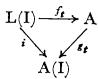
\includegraphics[keepaspectratio]{images/part001_16682a88.jpg}}

其中 \(i\) 是典范单射， \(f_{t}\) 是由 \(\pmb{t}\) 定义的李代数同态，而 \(g_{t}\) 是使得 \(g_{t}(i) = t_{i}\) （对 \(i\in I\) ）的幺代数同态。由于 \(g_{t}\circ i\) 与 \(f_{t}\) 在 I 上一致，该图表是交换的。由此得出，若 \(\mathrm{P}\in \mathrm{L}(\mathrm{I})\) ，则 § 2 no. 4 中定义的元素 \(\mathrm{P}((t_i)_{i\in I})\) 与《代数》第 III 章 § 2 no. 8 例 2 中定义的元素 \(\mathrm{P}((t_i)_{i\in I})\) 一致。

\subsection{\texorpdfstring{\(A^{+}(\mathrm{X})\) 到 \(\mathrm{L}(\mathrm{X})\) 上的投影}{A+ (X) 到 L(X) 上的投影}}

设 \(\pi\) 是 \(A^{+}(X)\) 到 \(L(X)\) 中的由下式定义的线性映射

\[
\pi (x _ {1} \dots x _ {n}) = (\mathrm{ad} (x _ {1}) \circ \dots \circ \mathrm{ad} (x _ {n - 1})) (x _ {n})\tag{3}
\]

其中 X 中的 \(n \geqslant 1, x_1, \ldots, x_n\) 。

命题 1. (a) 限制 \(\pi_0\) （即 \(\pi\) 在 \(\mathrm{L}(\mathbf{X})\) 上的限制）是 \(\mathrm{L}(\mathbf{X})\) 的一个导子。

\begin{enumerate}
\def\labelenumi{(\alph{enumi})}
\setcounter{enumi}{1}
\item
  对每个整数 \(n \geqslant 1\) 以及一切 \(u\) （属于 \(\mathbf{L}^n(\mathbf{X})\) ）， \(\pi(\mathbf{u}) = n.u.\)
\item
  设 E 是模 L(X) 的自同态代数， \(\theta\) 是 A(X) 到 E 中的一个同态，使得 \(\theta(x) = \operatorname{ad} x\) （对一切 \(x \in X\) ）。 \(\theta\) 在 L(X) 上的限制是 L(X) 到 E 中的一个李代数同态，它在 X 上与 L(X) 的伴随表示一致，从而
\end{enumerate}

\[
\theta (u). v = [ u, v ] \quad \text { for   } u, v \text {   in   } L (X).\tag{4}
\]

设 \(a\) 属于 \(\mathrm{A}(\mathrm{X})\) ， \(b\) 属于 \(\mathrm{A}^{+}(\mathrm{X})\) ；则

\[
\pi (a. b) = \theta (a). \pi (b).\tag{5}
\]

只需考虑 \(a = x_{1} \ldots x_{p}\) 、 \(b = x_{p+1} \ldots x_{p+q}\) （其中 \(p \geqslant 0\) ）、 \(q \geqslant 1\) 以及 \(x_{1}, \ldots, x_{p+q}\) （属于 \(\mathbf{X}\) ）的情形；但这时 (5) 由 (3) 立即得出，因为 \(\theta(x) = \operatorname{ad} x\) （对 \(x \in \mathbf{X}\) ）。

设 \(u\) 与 \(v\) 属于 \(\mathbf{L}(\mathbf{X})\) ；由 (4) 与 (5)，

\[
\begin{array}{r l} \pi_ {0} ([ u, v ]) & = \pi (u v - v u) = \theta (u). \pi (v) - \theta (v). \pi (u) \\ & = [ u, \pi (v) ] - [ v, \pi (u) ] = [ u, \pi_ {0} (v) ] + [ \pi_ {0} (u), v ], \end{array}
\]

因此 \(\pi_0\) 是 L(X) 的一个导子。

\begin{enumerate}
\def\labelenumi{(\alph{enumi})}
\setcounter{enumi}{1}
\tightlist
\item
  设 \(\pi_1\) 是模 \(\mathrm{L}(\mathbf{X})\) 的这样一个自同态：它在 \(\mathrm{L}^n (\mathbf{X})\) 上与用整数 \(n\geqslant 1\) 作乘法一致。公式 \([\mathrm{L}^n (\mathbf{X}),\mathrm{L}^m (\mathbf{X})]\subset \mathrm{L}^{n + m}(\mathrm{X})\) 表明 \(\pi_{1}\) 是一个导子 (《代数》， 第 III 章， § 10， no. 3， 例 6)。导子 \(\pi_1 - \pi_0\) （\(\mathrm{L}(\mathbf{X})\) 的）在 \(\mathbf{X}\) 上为零，并且由于 \(\mathbf{X}\) 生成 \(\mathrm{L}(\mathbf{X}),\pi_0 = \pi_1\) ，由此得 (b)。
\end{enumerate}

推论. 假设 K 是一个 Q-代数。设 P 是 \(A^{+}(X)\) 到其自身的线性映射，使得

\[
\mathrm{P} \left(x _ {1} \dots x _ {n}\right) = \frac {1}{n} (\operatorname{ad} x _ {1} \circ \dots \circ \operatorname{ad} x _ {n - 1}) (x _ {n})\tag{6}
\]

其中 \(n \geqslant 1\) 与 \(x_1, \ldots, x_n\) 都属于 \(\mathbf{X}\) 。那么 \(\mathbf{P}\) 是 \(\mathbf{A}^+(\mathbf{X})\) 到 \(\mathbf{L}(\mathbf{X})\) 上的一个投影。

\(\mathbf{P}\) 的像包含在 \(\mathrm{L}(\mathrm{X})\) 中。此外，对一切 \(n \geqslant 1\) 以及一切 \(u\) （属于 \(\mathrm{L}^n (\mathrm{X})\) ），有 \(\mathrm{P}(u) = \frac{1}{n}\pi (u)\) ，从而由命题 1 得 \(\mathrm{P}(u) = u\) 。由于

\[
\mathrm{L} (\mathrm{X}) = \sum_ {n \geqslant 1} \mathrm{L} ^ {n} (\mathrm{X}),
\]

我们看出 P 在 L(X) 上的限制是恒同映射。

注. 假设 K 是一个特征为零的域，并设 Q 是与 U(L(X)) 的典范分次相伴的、A(X) = U(L(X)) 到 L(X) 上的投影，参见 § 1 no. 5。对 \(\alpha \in \mathbf{N}^{(\mathbf{X})}\) ，有 Q(A \(^\alpha\) (X)) ⊂ L \(^\alpha\) (X)。因为只需验证 Q 的像与核都是 A(X) 的带有 N 型 \(^\alpha\) 分次的分次子模。这对像是显然的，因为它等于 L(X)。另一方面，设 n 是一个整数 \(\geqslant\) 1。A(X) 的由诸 \(y^n\) （其中 \(y \in L\) (X)）生成的向量子空间等于 A(X) 的由诸 \(\sum_{\sigma \in \mathcal{E}_n} y_{\sigma(1)} y_{\sigma(2)} \ldots y_{\sigma(n)}\) （其中 \(y_1, y_2, \ldots, y_n\) 是 L(X) 的齐次元素）生成的向量子空间；于是这个子空间是 A(X) 的一个分次子模。

（注意，若 \(\operatorname{Card}(\mathbf{X}) \geqslant 2\) ，则投影 \(\mathbf{P}\) 与 \(\mathbf{Q}\) 在 \(\mathbf{A}^{+}(\mathbf{X})\) 上并不一致。因为设 \(x, y\) 属于 \(\mathbf{X}\) 且 \(x \neq y\) ，并写

\[
z = x [ x, y ] + [ x, y ] x = x ^ {2} y - y x ^ {2}.
\]

则 \(\mathbf{Q}(z) = 0\) 且 \(\mathrm{P}(z) = \frac{1}{3}[x, [x,y]] \neq 0\) ，参见 § 2 no. 10 的例以及 no. 11 的定理 1。）

\subsection{L(X) 的齐次分量的维数}

设 X 是一个集合， \(\alpha\) 是 \(\mathbf{N}^{(X)}\) 的一个元素，d 是一个 >0 的整数。我们记 \(d|\alpha\) ，如果存在 \(\beta\in\mathbf{N}^{(X)}\) 使得 \(\alpha=d\beta\) 。这时唯一的元素 \(\beta\) 记作 \(\alpha/d\) 。

引理 1. 设 \(n\) 是一个整数 \(>0\) ， \(T_1, \ldots, T_n\) 是不定元， \(u_1, \ldots, u_n\) 是 \(\mathbf{Z}\) 的元素。设 \((c(\alpha))_{\alpha \in \mathbf{N}^n - \{0\}}\) 是 \(\mathbf{Z}\) 的元素的一个族，使得

\[
1 - \sum_ {i = 1} ^ {n} u _ {i} T _ {i} = \prod_ {\alpha \neq 0} (1 - T ^ {\alpha}) ^ {c (\alpha)}.\tag{7}
\]

对一切 \(\alpha \in \mathbf{N}^n - \{0\}\) ，

\[
c (\alpha) = \frac {1}{| \alpha |} \sum_ {d | \alpha} \mu (d) \frac {(| \alpha | / d) !}{(\alpha / d) !} u ^ {\alpha / d}\tag{8}
\]

其中 \(\mu\) 是 Möbius 函数（附录）。

在两边取对数后 (《代数》， 第 IV 章， § 6， no. 9)，公式 (7) 等价于：

\[
\log \left(1 - \sum_ {i = 1} ^ {n} u _ {i} T _ {i}\right) = \sum_ {\alpha \neq 0} c (\alpha) \log (1 - T ^ {\alpha}).\tag{9}
\]

而

\[
\begin{array}{r l} - \log \left(1 - \sum_ {i = 1} ^ {n} u _ {i} \mathrm{T} _ {i}\right) & = \sum_ {j \geqslant 1} \frac {1}{j} \left(\sum_ {i = 1} ^ {n} u _ {i} \mathrm{T} _ {i}\right) ^ {j} \\ & = \sum_ {j \geqslant 1} \frac {1}{j} \sum_ {| \beta | = j} \frac {| \beta | !}{\beta !} u ^ {\beta} \mathrm{T} ^ {\beta} \\ & = \sum_ {| \beta | > 0} \frac {1}{| \beta |} \frac {| \beta | !}{\beta !} u ^ {\beta} \mathrm{T} ^ {\beta}. \end{array}\tag{10}
\]

另一方面

\[
\begin{array}{r l} - \sum_ {\alpha \neq 0} c (\alpha) \log (1 - T ^ {\alpha}) & = \sum_ {| \alpha | > 0, k \geqslant 1} \frac {1}{k} c (\alpha) T ^ {k \alpha} \\ & = \sum_ {| \beta | > 0, k | \beta} \frac {1}{k} c \left(\frac {\beta}{k}\right) T ^ {\beta}. \end{array}\tag{11}
\]

因此 (7) 等价于

\[
\sum_ {k \mid \beta} \left| \frac {\beta}{k} \right| c \left(\frac {\beta}{k}\right) = \frac {| \beta | !}{\beta !} u ^ {\beta} \quad \text { for   all } \beta \in \mathbf {N} ^ {n} - \{0 \}.\tag{12}
\]

设 \(\Lambda\) 是由 \((\lambda_1, \lambda_2, \ldots, \lambda_n) \in \mathbf{N}^n - \{0\}\) 组成的集合，其中 \(\lambda_1, \lambda_2, \ldots, \lambda_n\) 的最大公因子等于 1。 \(\mathbf{N}^n - \{0\}\) 的每个元素都可以唯一地写成

形式 \(m\lambda\) ，其中 \(m\) 是一个整数 \(\geqslant 1\) 且 \(\lambda \in \Lambda\) 。条件 (12) 等价于

\[
\sum_ {k \mid m} \left| \frac {m \lambda}{k} \right| c \left(\frac {m \lambda}{k}\right) = \frac {(m | \lambda |) !}{(m \lambda) !} u ^ {m \lambda} \quad \text { for   all } \lambda \in \Lambda \text { and   all } m \geqslant 1.\tag{13}
\]

由 Möbius 反演公式（附录），条件 (13) 等价于

\[
\left| m \lambda \right| c (m \lambda) = \sum_ {d \mid m} \mu (d) \frac {\left| \frac {m \lambda}{d} \right| !}{\left(\frac {m \lambda}{d}\right) !} u ^ {\frac {m \lambda}{d}}\tag{14}
\]

其中一切 \(\lambda\in\Lambda\) 与一切 \(m\geqslant1\) 。

定理 2. 设 X 是一个有限集，并且 \(n = \operatorname{Card}(X)\) 。

\begin{enumerate}
\def\labelenumi{(\alph{enumi})}
\tightlist
\item
  对每个整数 \(r \geqslant 1\) ，K-模 \(\mathbf{L}^r(\mathbf{X})\) 都是自由的，其秩为
\end{enumerate}

\[
c (r) = \frac {1}{r} \sum_ {d | r} \mu (d) n ^ {r / d},\tag{15}
\]

其中 μ 是 Möbius 函数。

\begin{enumerate}
\def\labelenumi{(\alph{enumi})}
\setcounter{enumi}{1}
\tightlist
\item
  对一切 \(\alpha \in \mathbf{N}^{(\mathbf{X})} - \{0\}\) ，K-模 \(\mathbf{L}^{\alpha}(\mathbf{X})\) ( \(\S 2\) ， no. 6) 都是自由的，其秩为
\end{enumerate}

\[
c (\alpha) = \frac {1}{| \alpha |} \sum_ {d | \alpha} \mu (d) \frac {(| \alpha | / d) !}{(\alpha / d) !}.\tag{16}
\]

我们已经知道，模 \(L^{r}(\mathbf{X})\) （其中 \(r \in \mathbf{N}\) ）与 \(L^{\alpha}(\mathbf{X})\) （其中 \(\alpha \in \mathbf{N}^{\mathbf{X}}\) ）都是自由的 (§ 2， no. 11， 定理 1 的推论)。考察 A(X) 的多重分次 \((A^{\alpha}(X))_{\alpha \in \mathbf{N}^{\mathbf{X}}}\) ，它由典范同态 \(\phi\) （从 Mo(X) 到 \(\mathbf{N}^{\mathbf{X}}\) 中）所定义 (《代数》， 第 III 章， § 3， no. 1， 例 3)；于是由 no. 1 的注 3 有 \(A^{\alpha}(\mathbf{X}) \cap L(\mathbf{X}) = L^{\alpha}(\mathbf{X})\) 。对 \(\alpha \in \mathbf{N}^{\mathbf{X}}\) ，K-模 \(A^{\alpha}(\mathbf{X})\) 以这样的字的集合为基：X 的每个字母 \(x\) 在其中出现 \(\alpha(x)\) 次。设 \(d(\alpha)\) 是这些字的个数，即 \(A^{\alpha}(\mathbf{X})\) 的秩；我们将以两种不同的方式计算形式幂级数

它由

\[
\mathbf {P} ((\mathrm{T} _ {x}) _ {x \in \mathbf {X}}) \in \mathbf {Z} [ [ (\mathrm{T} _ {x}) _ {x \in \mathbf {X}} ] ]\tag{17}
\]

\[
\mathrm{P} (\mathrm{T}) = \sum_ {\alpha \in \mathbf {N} ^ {\mathbf {X}}} d (\alpha) \mathrm{T} ^ {\alpha}.
\]

\begin{enumerate}
\def\labelenumi{(\arabic{enumi})}
\tightlist
\item
  我们有
\end{enumerate}

\[
\mathrm{P} (\mathrm{T}) = \sum_ {m \in \mathrm{Mo} (\mathrm{X})} \mathrm{T} ^ {\phi (m)} = \sum_ {r = 0} ^ {\infty} \sum_ {x _ {1}, \dots , x _ {r}} \mathrm{T} _ {x _ {1}} \dots \mathrm{T} _ {x _ {r}} = \sum_ {r = 0} ^ {\infty} \left(\sum_ {x \in \mathrm{X}} \mathrm{T} _ {x}\right) ^ {r}
\]

从而

\[
\mathrm{P} (\mathrm{T}) = \left(1 - \sum_ {x \in \mathbf {X}} \mathrm{T} _ {x}\right) ^ {- 1}.\tag{18}
\]

\begin{enumerate}
\def\labelenumi{(\arabic{enumi})}
\setcounter{enumi}{1}
\tightlist
\item
  对一切 \(\alpha \in \mathbf{N}^{\mathbf{X}} - \{0\}\) ，设 \((e_{\alpha,j})_{1 \leqslant j \leqslant c(\alpha)}\) 是 \(\mathrm{L}^{\alpha}(\mathbf{X})\) 的一个基，并给集合 I 一个全序，I 由有序对 \((\alpha, j)\) （满足 \(\alpha \in \mathbf{N}^{\mathbf{X}} - \{0\}\) 且 \(1 \leqslant j \leqslant c(\alpha)\) ）组成。由 no. 1 的定理 1 与 Poincaré-Birkhoff-Witt 定理 (第 I 章， § 2， no. 7， 定理 1 的推论 3)，诸元素
\end{enumerate}

\[
y _ {m} = \prod_ {(\alpha , j) \in \mathbb {I}} (e _ {\alpha , j}) ^ {m (\alpha , j)},
\]

（其中指标 \(\pmb{m}\) 取遍 \(\mathbf{N}^{(I)}\) ）构成 \(A(\mathbf{X})\) 的一个基。每个 \(y_{m}\) 都有一个多重次数 \(\sum_{(\alpha, j) \in I} \pmb{m}(\alpha, j)\alpha\) 。用 \(u(\pmb{m})\) 表示这个多重次数。由此得出

\[
\begin{array}{l} \mathrm{P(T)} = \sum_ {m \in \mathrm{N} ^ {(I)}} \mathrm{T} ^ {u (m)} = \sum_ {m \in \mathrm{N} ^ {(I)}} \prod_ {(\alpha , j) \in I} \mathrm{T} ^ {m (\alpha , j) \alpha} \\ = \prod_ {(\alpha , j) \in I} \sum_ {r = 0} ^ {\infty} \mathrm{T} ^ {r \alpha} = \prod_ {(\alpha , j) \in I} (1 - \mathrm{T} ^ {\alpha}) ^ {- 1}, \end{array}
\]

从而最后

\[
\mathrm{P} (\mathrm{T}) = \prod_ {\alpha \in \mathbf {N} ^ {\mathbf {X}} - \{0 \}} (1 - \mathrm{T} ^ {\alpha}) ^ {- c (\alpha)}.\tag{19}
\]

比较 (18) 与 (19)，我们得到

\[
1 - \sum_ {x \in \mathbf {X}} T _ {x} = \prod_ {\alpha \in \mathbf {N} ^ {\mathbf {X}} - \{0\}} (1 - T ^ {\alpha}) ^ {c (\alpha)}.\tag{20}
\]

于是引理 1 给出 (b)。

若现在在公式 (20) 中把同一个不定元 U 代入诸 \(T_{x}\) （对 \(x \in X\) ），则得到

\[
1 - n \mathrm{U} = \prod_ {\alpha \in \mathbf {N} ^ {\mathrm{X}} - \{0\}} (1 - \mathrm{U} ^ {| \alpha |}) ^ {c (\alpha)} = \prod_ {r > 0} (1 - \mathrm{U} ^ {r}) ^ {c (r)}.
\]

再次应用引理 1，我们推出 (a)。

例. 我们有

\[
\begin{array}{l l} c (1) = n, & c (2) = \frac {1}{2} (n ^ {2} - n), \qquad c (3) = \frac {1}{3} (n ^ {3} - n), \\ c (4) = \frac {1}{4} (n ^ {4} - n ^ {2}), & c (5) = \frac {1}{5} (n ^ {5} - n), \qquad c (6) = \frac {1}{6} (n ^ {6} - n ^ {3} - n ^ {2} + n). \end{array}
\]

注. 设 X 是一个集合并设 \(\alpha \in \mathbf{N}^{(X)}\) ；自由 K-模 \(\mathbf{L}^{\alpha}(X)\) 的秩也由公式 (16) 给出。这由定理 2 (b) 以及 § 2 no. 6 的命题 4 立即得出。

\section{中心滤过}

\subsection{实滤过}

定义 1. 设 G 是一个群。G 上的实滤过是指 G 的子群的一个族 \((\mathrm{G}_{\alpha})_{\alpha \in \mathbf{R}}\) ，使得

\[
\mathrm{G} _ {\alpha} = \bigcap_ {\beta <   \alpha} \mathrm{G} _ {\beta} \text {   for   all   } \alpha \in \mathbf {R}.\tag{1}
\]

公式 (1) 蕴涵 \(G_{\alpha} \subset G_{\beta}\) （对 \(\beta < \alpha\) ），因而族 \((\mathrm{G}_{\alpha})\) 是递减的。滤过 \((\mathrm{G}_{\alpha})\) 称为分离的，如果 \(\bigcap_{\alpha} G_{\alpha}\) 化为单位元素；称为穷竭的，如果 \(G = \bigcup_{\alpha} G_{\alpha}\) 。

注. 设 \((\mathrm{G}_n)_{n\in \mathbf{Z}}\) 是 G 的子群的一个递减序列。它是《交换代数》第 III 章 § 2 no. 1 定义 1 意义下的递减滤过。对每个整数 \(n\) 以及每个 \(\alpha\) （取自区间 \(]n - 1,n]\) ，即 \(\mathbf{R}\) 中的一个区间），我们记 \(\mathrm{H}_{\alpha} = \mathrm{G}_{n}\) ，特别地 \(\mathrm{H}_n = \mathrm{G}_n\) 。立即可见我们这样就得到 G 上的一个实滤过 \((\mathrm{H}_{\alpha})_{\alpha \in \mathbf{R}}\) ；这样的滤过将称为整滤过。因此《交换代数》第 III 章 § 2 意义下的递减滤过可以与整滤过等同。

设 A 是一个代数；A 的加法群上的实滤过 \((\mathrm{A}_{\alpha})\) 称为与该代数结构相容，如果 \(\mathrm{A}_{\alpha}.\mathrm{A}_{\beta}\subset \mathrm{A}_{\alpha +\beta}\) （对 R 中的 \(\alpha ,\beta\) ），且 \(\mathrm{K.A}_{\alpha}\subset \mathrm{A}_{\alpha}\) （对 \(\alpha \in \mathbf{R}\) ）。若滤过是穷竭的，则 \((\mathrm{A}_{\alpha})\) 是 A 上与该代数结构相容的拓扑之下 0 的一个邻域基本系。设 B 是一个幺代数；B 的加法群上的实滤过 \((\mathrm{B}_{\alpha})\) 称为与该幺代数结构相容，如果它与该代数结构相容并且 \(1\in \mathrm{B}_0\) 。

\subsection{阶函数}

设 \(G\) 是一个以 \(e\) 为单位元素的群。设 \((\mathbf{G}_{\alpha})\) 是 \(G\) 上的一个实滤过。对一切 \(x\) （属于 \(G\) ），用 \(I_x\) 表示实数 \(\alpha\) 组成的集合，其中实数满足 \(x \in G_{\alpha}\) 。若 \(\alpha \in I_x\) 且 \(\beta < \alpha\) ，则 \(\beta \in I_x\) ，因而 \(I_x\) 是一个区间 (《一般拓扑学》， 第 IV 章， § 2， no. 4， 命题 1)。利用关系式 (1)，我们看出 \(I_x\) 当其上确界有限时含有该上确界。因此 \(I_x\) 具有形式 \(] - \infty\) 、 \(v(x)] \cap R\) ，其中 \(v(x) \in \overline{\mathbf{R}}\) ；我们有 \(v(x) = \sup(\alpha \mid x \in G_{\alpha})\) 。

映射 \(v\) （从 \(G\) 到 \(\overline{\mathbf{R}}\) 中）称为与实滤过 \((G_{\alpha})\) 相伴的阶函数，而 \(v(x)\) 称为 \(x\) 的阶。这个映射具有下列性质：

\begin{enumerate}
\def\labelenumi{(\alph{enumi})}
\item
  对 \(x \in \mathbf{G}\) 与 \(\alpha \in \mathbf{R}\) ，关系式 \(x \in \mathbf{G}_{\alpha}\) 与 \(v(x) \geqslant \alpha\) 等价。
\item
  对 G 中的 x、y，
\end{enumerate}

\begin{enumerate}
\def\labelenumi{(\arabic{enumi})}
\setcounter{enumi}{1}
\tightlist
\item
\end{enumerate}

\[
v (x ^ {- 1}) = v (x), \quad v (e) = + \infty .\tag{2}
\]

\[
v (x y) \geqslant \inf (v (x), v (y)).\tag{3}
\]

此外，当 \(v(x) > v(y)\) 时 (3) 中取等号。

\begin{enumerate}
\def\labelenumi{(\alph{enumi})}
\setcounter{enumi}{2}
\tightlist
\item
  对一切 \(\alpha \in \mathbf{R}\) ，用 \(\mathrm{G}_{\alpha}^{+}\) 表示 \(x \in \mathrm{G}\) 组成的集合，其中 \(v(x) > \alpha\) 。那么 \(\mathrm{G}_{\alpha}^{+} = \bigcup_{\beta > \alpha} \mathrm{G}_{\beta}\) ，特别地 \(\mathrm{G}_{\alpha}^{+}\) 是 \(\mathrm{G}\) 的一个子群。
\end{enumerate}

反之，设 \(v\) 是 \(G\) 到 \(\overline{\mathbf{R}}\) 中的满足关系式 (2) 与 (3) 的映射。对一切 \(\alpha \in \mathbf{R}\) ，令 \(G_{\alpha}\) 为 \(x \in G\) 组成的集合，其中 \(v(x) \geqslant \alpha\) 。那么 \((G_{\alpha})_{\alpha \in \mathbf{R}}\) 是 \(G\) 的一个实滤过，而 \(v\) 是与这个滤过相伴的阶函数。

滤过 \((\mathbf{G}_{\alpha})\) 为整滤过，当且仅当 \(v\) 把 \(\mathbf{G}\) 映到 \(\mathbf{Z} \cup \{+\infty, -\infty\}\) 中。它为穷竭的（相应地，分离的），当且仅当 \(v^{-1}(-\infty) = \varnothing\) （相应地， \(v^{-1}(+\infty) = \{e\}\) ）。

设 A 是一个 K-代数（相应地，幺 K-代数）。由上所述，关系式

\[
" x \in \mathrm{A} _ {\alpha} \Leftrightarrow v (x) \geqslant \alpha \quad \text { for } x \in \mathrm{A} \text { and } \alpha \in \mathbf {R}"
\]

定义了 A 上与代数（相应地，幺代数）结构相容的穷竭实滤过 \((\mathbf{A}_{\alpha})_{\alpha\in\mathbf{R}}\) 的集合到映射 \(v: A \to \overline{\mathbf{R}}\) 组成的集合上的一个双射，这些映射不取值 \(-\infty\) 且满足下列公理 (4) 至 (7)（相应地， (4) 至 (8)）：

\begin{enumerate}
\def\labelenumi{(\arabic{enumi})}
\setcounter{enumi}{3}
\tightlist
\item
\end{enumerate}

\[
v (x + y) \geqslant \inf (v (x), v (y)) \quad (x, y \text {   in   A })\tag{5}
\]

\[
v (- x) = v (x) \quad (x \in \mathrm{A})\tag{6}
\]

\[
v (\lambda x) \geqslant v (x) \quad (\lambda \in \mathrm{K}, x \in \mathrm{A})\tag{7}
\]

\[
v (x y) \geqslant v (x) + v (y) \quad (x, y \text {   in   A })\tag{8}
\]

\[
v (1) \geqslant 0.
\]

注. 若 \(v(x)\) 不恒等于 \(+\infty\) ，则条件 (7) 与 (8) 蕴涵 \(v(1) = 0\) 。

\subsection{与滤过代数相伴的分次代数}

设 G 是一个带实滤过 \((G_{\alpha})_{\alpha \in \mathbb{R}}\) 的交换群。如同前面我们记

\[
\mathrm{G} _ {\alpha} ^ {+} = \bigcup_ {\beta > \alpha} \mathrm{G} _ {\beta};\tag{9}
\]

显然 \(\mathrm{G}_{\alpha}^{+}\) 是 \(\mathrm{G}_{\alpha}\) 的一个子群。我们记 \(\mathrm{gr}_{\alpha}(\mathrm{G}) = \mathrm{G}_{\alpha} / \mathrm{G}_{\alpha}^{+}\) ，并且

\[
\operatorname{gr} (\mathrm{G}) = \bigoplus_ {\alpha \in \mathbf {R}} \operatorname{gr} _ {\alpha} (\mathrm{G}).
\]

与滤过群 G 相伴的分次群是群 \(\operatorname{gr}(G)\) ，带其自然的 R 型分次。

注. 当滤过 \((\mathrm{G}_{\alpha})\) 是整滤过时， \(\mathrm{gr}_{\alpha}(\mathrm{G}) = \{0\}\) （对非整的 \(\alpha\) ），而 \(\mathrm{gr}_n(\mathrm{G}) = \mathrm{G}_n / \mathrm{G}_{n - 1}\) （对每个整数 \(n\) ）。因此相伴分次群的定义与《交换代数》第 III 章 § 2 no. 3 中的定义本质上是一致的。

设 \(\mathbf{A}\) 是一个代数（相应地，幺代数）， \((\mathbf{A}_{\alpha})_{\alpha \in \mathbb{R}}\) 是一个与代数（相应地，幺代数）结构相容的实滤过 (no. 1)。那么

\[
\mathrm{A} _ {\alpha}. \mathrm{A} _ {\beta} \subset \mathrm{A} _ {\alpha + \beta}, \quad \mathrm{A} _ {\alpha} ^ {+}. \mathrm{A} _ {\beta} + \mathrm{A} _ {\alpha}. \mathrm{A} _ {\beta} ^ {+} \subset \mathrm{A} _ {\alpha + \beta} ^ {+},
\]

，并且由 A 上乘法的限制所给出的 \(A_{\alpha} \times A_{\beta}\) 到 \(A_{\alpha+\beta}\) 中的双线性映射在取商后定义了一个双线性映射

\[
\operatorname{gr} _ {\alpha} (\mathrm{A}) \times \operatorname{gr} _ {\beta} (\mathrm{A}) \rightarrow \operatorname{gr} _ {\alpha + \beta} (\mathrm{A}).
\]

我们得到 \(\mathrm{gr}(\mathbf{A}) \times \mathrm{gr}(\mathbf{A})\) 到 \(\mathrm{gr}(\mathbf{A})\) 中的一个双线性映射，它使后者成为一个 R 型分次代数（相应地，幺分次代数）。若 A 是一个结合代数（相应地，交换代数，相应地，李代数），则 \(\mathrm{gr}(\mathbf{A})\) 亦然。

\subsection{群上的中心滤过}

定义 2. 设 G 是一个群。G 上的实滤过 \((\mathrm{G}_{\alpha})\) 称为中心的，如果 \(\mathrm{G} = \bigcup_{\alpha >0}\mathrm{G}_{\alpha}\) ，并且换位子 \((x,y) = x^{-1}y^{-1}xy\) ——它由一个元素 \(x\) （属于 \(\mathrm{G}_{\alpha}\) ）与一个元素 \(y\) （属于 \(\mathrm{G}_{\beta}\) ）构成——属于 \(\mathrm{G}_{\alpha +\beta}\) 。

用阶函数 v 来说，上述定义转换为关系式

\[
v (x) > 0, \quad v ((x, y)) \geqslant v (x) + v (y) \quad \text { for   all } x, y \text { in } G.\tag{10}
\]

我们推出 \(v((x,y)) > v(x)\) （若 \(v(x) \neq +\infty\) ）；若记 \(x^y = y^{-1}xy\) （参见《代数》， 第 I 章， § 6， no. 2），则 \(x^y = x.(x,y)\) ，从而

\[
v (x ^ {y}) = v (x).\tag{11}
\]

这个关系式表达了如下事实：G 的诸子群 \(G_{\alpha}\) 中的每一个都是正规的。诸 \(G_{\alpha}\) 构成与 G 上群结构相容的一个拓扑 (《一般拓扑学》， 第 III 章， § 1， no. 2， 例) 之下 e 的一个邻域基本系，该拓扑称为由滤过 ( \(G_{\alpha}\) ) 所定义。

在本 no. 的其余部分，G 表示一个带中心滤过 \((G_{\alpha})\) 的群。对一切 \(\alpha \in R\) ，我们用下式定义 G 的子群 \(G_{\alpha}^{+}\) ：

\[
\mathrm{G} _ {\alpha} ^ {+} = \bigcup_ {\beta > \alpha} \mathrm{G} _ {\beta}.\tag{12}
\]

特别地， \(G_{\alpha}^{+} = G_{\alpha} = G\) （对 \(\alpha \leqslant 0\) ）。回顾若 A 与 B 是 G 的两个子群，则 (A, B) 表示由换位子 \((a, b)\) （满足 \(a \in A\) 且 \(b \in B\) ）生成的 G 的子群。用这个记号，我们有公式

\begin{enumerate}
\def\labelenumi{(\arabic{enumi})}
\setcounter{enumi}{12}
\tightlist
\item
\end{enumerate}

\[
\left(\mathrm{G} _ {\alpha}, \mathrm{G} _ {\beta}\right) \subset \mathrm{G} _ {\alpha + \beta}\tag{13}
\]

\[
\left(\mathrm{G} _ {\alpha} ^ {+}, \mathrm{G} _ {\beta}\right) \subset \mathrm{G} _ {\alpha + \beta} ^ {+}\tag{13'}
\]

\[
(G, G _ {\alpha}) \subset G _ {\alpha} ^ {+}.\tag{14}
\]

由 (14)， \(\mathrm{G}_{\alpha}^{+}\) 是 \(\mathrm{G}_{\alpha}\) 的一个正规子群（对一切 \(\alpha \in \mathbf{R}\) ），并且商群 \(\mathrm{gr}_{\alpha}(\mathrm{G}) = \mathrm{G}_{\alpha} / \mathrm{G}_{\alpha}^{+}\) 是交换的。我们记 \(\mathrm{gr}(\mathrm{G}) = \bigoplus_{\alpha \in \mathbb{R}}\mathrm{gr}_{\alpha}(\mathrm{G})\) ，并给这个群赋予 \(\mathbf{R}\) 型分次，其中 \(\mathrm{gr}_{\alpha}(\mathrm{G})\) 由 \(\alpha\) 次的元素组成。于是 \(\mathrm{gr}_{\alpha}(\mathrm{G}) = \{0\}\) （对 \(\alpha \leqslant 0\) ）。

命题 1. (i) 设 \(\alpha, \beta\) 属于 \(\mathbf{R}\) 。存在一个双加性映射

\[
\phi_ {\alpha \beta}: \operatorname{gr} _ {\alpha} (\mathrm{G}) \times \operatorname{gr} _ {\beta} (\mathrm{G}) \rightarrow \operatorname{gr} _ {\alpha + \beta} (\mathrm{G})
\]

它把 \((x\mathrm{G}_{\alpha}^{+},y\mathrm{G}_{\beta}^{+})\) 映到 \((x,y)\mathrm{G}_{\alpha +\beta}^{+}\) 上

\begin{enumerate}
\def\labelenumi{(\roman{enumi})}
\setcounter{enumi}{1}
\item
  设 \(\phi\) 是 \(\operatorname{gr}(\mathbf{G}) \times \operatorname{gr}(\mathbf{G})\) 到 \(\operatorname{gr}(\mathbf{G})\) 中的一个双加性映射，它在 \(\operatorname{gr}_{\alpha}(\mathbf{G}) \times \operatorname{gr}_{\beta}(\mathbf{G})\) 上的限制是 \(\phi_{\alpha \beta}\) （对每个有序对 \((\alpha, \beta)\) ）。映射 \(\phi\) 给 \(\operatorname{gr}(\mathbf{G})\) 一个李 Z-代数结构。
\item
  回顾恒等式
\end{enumerate}

\[
(x x ^ {\prime}, y) = (x, y) ^ {x ^ {\prime}} \left(x ^ {\prime}, y\right)\tag{15}
\]

其中 \(x, x', y\) 属于 \(\mathbf{G}\) (《代数》， 第 I 章， § 6， no. 2， 公式 (4 bis))。

对 \(x \in G_{\alpha}\) 与 \(y \in G_{\beta}\) ，模 \(G_{\alpha + \beta}^{+}\) 的类（元素 \((x, y)\) 取自 \(G_{\alpha + \beta}\) ）将记作 \(f(x, y)\) 。对 \(a\) （属于 \(G_{\alpha + \beta}\) ）与 \(x'\) （属于 \(G, a^{-1}.a^{x'} = (a, x') \in G_{\alpha + \beta}^{+}\) ）；特别地， \(f(x, y)\) 等于模 \(G_{\alpha + \beta}^{+}\) 的类（元素 \((x, y)^{x'}\) 的类）。因此公式 (15) 蕴涵

\[
f (x x ^ {\prime}, y) = f (x, y) f (x ^ {\prime}, y).\tag{16}
\]

而 \((y, x) = (x, y)^{-1}\) ，从而

\[
f (y, x) = f (x, y) ^ {- 1}.\tag{17}
\]

由 (16) 与 (17) 我们推出

\[
f (x, y y ^ {\prime}) = f (x, y) f (x, y ^ {\prime}).\tag{18}
\]

我们必须证明映射 \(f\colon \mathrm{G}_{\alpha}\times \mathrm{G}_{\beta}\to \mathrm{gr}_{\alpha +\beta}(\mathrm{G})\) 在取商后定义一个映射 \(\phi_{\alpha \beta}\colon \mathrm{gr}_{\alpha}(\mathrm{G})\times \mathrm{gr}_{\beta}(\mathrm{G})\to \mathrm{gr}_{\alpha +\beta}(\mathrm{G})\) 。由 (16) 与 (18)，只需证明 \(f(x,y) = 0\) （当 \(x\in \mathrm{G}_{\alpha}^{+}\) 或 \(y\in \mathrm{G}_{\beta}^{+}\) 时），而这由 (13') 得出。

\begin{enumerate}
\def\labelenumi{(\roman{enumi})}
\setcounter{enumi}{1}
\tightlist
\item
  由于 \((x, x) = e\) ，由 (17) 推出 \(\phi\) 是一个交错的双 \(\mathbf{Z}\) -线性映射。因此剩下要证明的是，对 \(u \in \mathrm{gr}_{\alpha}(\mathrm{G})\) 、 \(v \in \mathrm{gr}_{\beta}(\mathrm{G})\) 与 \(w \in \mathrm{gr}_{\gamma}(\mathrm{G})\) ，
\end{enumerate}

\[
\phi (u, \phi (v, w)) + \phi (v, \phi (w, u)) + \phi (w, \phi (u, v)) = 0.\tag{19}
\]

设 \(x \in G_{\alpha}, y \in G_{\beta}\) 与 \(z \in G_{\gamma}\) 是分别表示 \(u, v\) 与 \(w\) 的元素。我们知道 \(x^{y}\) 与 \(x\) 是 \(G_{\alpha}\) 的两个模 \(G_{\alpha}^{+}\) 同余的元素，因而 \(x^{y}\) 是 \(u\) 在 \(G_{\alpha}\) 中的一个代表；由于 \((y, z)\) 是 \(\phi(v, w)\) 在 \(G_{\beta + \gamma}\) 中的一个代表，我们看出 \((x^{y}, (y, z))\) 是 \(\phi(u, \phi(v, w))\) 在 \(G_{\alpha + \beta + \gamma}\) 中的一个代表。通过轮换，我们看出 \((y^{z}, (z, x))\) 与 \((z^{x}, (x, y))\) 分别表示 \(\phi(v, \phi(w, u))\) 与 \(\phi(w, \phi(u, v))\) （在 \(G_{\alpha + \beta + \gamma}\) 中）。于是关系式 (19) 是下列恒等式 (《代数》， 第 I 章， § 6， no. 2， 公式 (15)) 的推论：

\[
\left(x ^ {y}, (y, z)\right). \left(y ^ {z}, (z, x)\right). \left(z ^ {x}, (x, y)\right) = e.\tag{20}
\]

在命题 1 中定义的李代数 \(\mathrm{gr}(\mathbf{G})\) （环 \(\mathbf{Z}\) 上的）称为与滤过群 \(\mathbf{G}\) 相伴的分次李代数。

\subsection{中心滤过的一个例子}

设 \(\mathbf{A}\) 是一个带幺代数滤过 \((\mathbf{A}_{\alpha})\) 的幺结合代数，使得 \(\mathbf{A}_{0} = \mathbf{A}\) ；那么 \(\mathbf{A}_{\alpha}\) 是 \(\mathbf{A}\) 的一个双边理想（对一切 \(\alpha \in \mathbf{R}\) ）。用 \(\mathbf{A}^*\) 表示 \(\mathbf{A}\) 的可逆元素组成的乘法群。对一切 \(\alpha > 0\) ，用 \(\Gamma_{\alpha}\) 表示 \(x \in \mathbf{A}^*\) 组成的集合，其中 \(x - 1 \in \mathbf{A}_{\alpha}\) ；我们记 \(\Gamma = \bigcup_{\alpha > 0} \Gamma_{\alpha}\) 与 \(\Gamma_{\beta} = \Gamma\) （对 \(\beta \leqslant 0\) ）。

命题 2. 集合 \(\Gamma\) 是 \(\mathbf{A}^*\) 的一个子群，并且 \((\Gamma_{\alpha})\) 是 \(\Gamma\) 上的一个中心滤过。

按构造有 \(\Gamma = \bigcup_{\alpha > 0} \Gamma_{\alpha}\) ，而关系式 \(\Gamma_{\alpha} = \bigcap_{\beta < \alpha} \Gamma_{\beta}\) 由 \(A_{\alpha} = \bigcap_{\beta < \alpha} A_{\beta}\) 得出。

我们证明 \(\Gamma_{\alpha}\) 是 \(\mathbf{A}^*\) 的一个子群。而 \(1 \in \Gamma_{\alpha}\) ；设 \(x, y\) 属于 \(\Gamma_{\alpha}\) ，从而 \(x - 1 \in \mathbf{A}_{\alpha}, y - 1 \in \mathbf{A}_{\alpha}\) 。由于 \(\mathbf{A}_{\alpha}\) 是 \(\mathbf{A}\) 的一个双边理想，公式

\begin{enumerate}
\def\labelenumi{(\arabic{enumi})}
\setcounter{enumi}{20}
\tightlist
\item
\end{enumerate}

\[
x y - 1 = (x - 1) (y - 1) + (x - 1) + (y - 1),\tag{21}
\]

\[
x ^ {- 1} - 1 = - x ^ {- 1} (x - 1),\tag{22}
\]

蕴涵 \(xy - 1 \in A_{\alpha}\) 与 \(x^{-1} - 1 \in A_{\alpha}\) ，从而 \(xy \in \Gamma_{\alpha}\) 且 \(x^{-1} \in \Gamma_{\alpha}\) 。

由于 \(\Gamma = \bigcup_{\alpha > 0} \Gamma_{\alpha}\) ，它是 \(A^{*}\) 的一个子群。

最后设 \(\alpha > 0, \beta > 0, x \in \Gamma_{\alpha}\) 与 \(y \in \Gamma_{\beta}\) 。设 \(x - 1 = \xi\) 与 \(y - 1 = \eta\) 。那么

\[
(x, y) - 1 = x ^ {- 1} y ^ {- 1} (\xi \eta - \eta \xi);\tag{23}
\]

由假设， \(\xi \in \mathbf{A}_{\alpha}\) 且 \(\eta \in \mathbf{A}_{\beta}\) ，从而 \(\xi \eta - \eta \xi \in \mathbf{A}_{\alpha + \beta}\) 。由于 \(\mathbf{A}_{\alpha + \beta}\) 是 \(\mathbf{A}, (x, y) - 1 \in \mathbf{A}_{\alpha + \beta}\) 的一个双边理想，由此得 \((x, y) \in \Gamma_{\alpha + \beta}\) 。

注. 设 \(\alpha \geqslant 0, \beta \geqslant 0\) 与 \(x \in \Gamma_{\alpha}, y \in \Gamma_{\beta}\) 。由公式 (21)、 (22) 与 (23)，

\begin{enumerate}
\def\labelenumi{(\arabic{enumi})}
\setcounter{enumi}{23}
\tightlist
\item
\end{enumerate}

\[
x ^ {- 1} - 1 \equiv - (x - 1) \quad \text { mod. } A _ {2 \alpha}\tag{24}
\]

\[
x y - 1 \equiv (x - 1) + (y - 1) \quad \text { mod. } A _ {\alpha + \beta}\tag{25}
\]

\[
(x, y) - 1 \equiv [ (x - 1), (y - 1) ] \mod A _ {\alpha + \beta + \inf (\alpha , \beta)}.\tag{26}
\]

例如我们证明 (26)。若 \(x - 1 = \xi\) 且 \(y - 1 = \eta\) ，则 (23) 给出：

\[
(x, y) - 1 - [ \xi , \eta ] = ((x ^ {- 1} - 1) + (y ^ {- 1} - 1) + (x ^ {- 1} - 1) (y ^ {- 1} - 1)) [ \xi , \eta ].
\]

而 \([\xi, \eta] \in \mathrm{A}_{\alpha + \beta}, (x^{-1} - 1) \in \mathrm{A}_{\alpha}, (y^{-1} - 1) \in \mathrm{A}_{\beta}\) ，由此得到 (26)。

设 \(G\) 是一个群， \(\rho: G \to \Gamma\) 是一个同态。对一切实数 \(\alpha\) ，我们记 \(G_{\alpha} = \rho^{-1}(\Gamma_{\alpha})\) 。由于 \((\Gamma_{\alpha})\) 是 \(\Gamma\) 上的一个中心滤过，立即可见 \((G_{\alpha})\) 是 \(G\) 上的一个中心滤过。

命题 3. (i) 对一切 \(\alpha \in \mathbf{R}\) ，存在唯一的群同态 \(g_{\alpha} \colon \mathrm{gr}_{\alpha}(\mathrm{G}) \to \mathrm{gr}_{\alpha}(\mathrm{A})\) ，它把模 \(\mathrm{G}_{\alpha}^{+}\) 类（元素 \(a \in \mathrm{G}_{\alpha}\) 的类）映到模 \(\mathrm{A}_{\alpha}^{+}\) 类（\(\rho(a) - 1\) 的类）。

\begin{enumerate}
\def\labelenumi{(\roman{enumi})}
\setcounter{enumi}{1}
\item
  设 \(g\) 是 \(\mathrm{gr}(\mathrm{G})\) 到 \(\mathrm{gr}(\mathrm{A})\) 中的群同态，它在 \(\mathrm{gr}_{\alpha}(\mathrm{G})\) 上的限制是 \(g_{\alpha}\) （对一切 \(\alpha\) ）。映射 \(g\) 是李 Z-代数的一个单同态。 (i) 设 \(\alpha > 0\) 。由假设，结论对一切 \(a\) （属于 \(\mathrm{G}_{\alpha}, \rho(a) - 1 \in \mathrm{A}_{\alpha}\) ）成立；用 \(p_{\alpha}(a)\) 表示 \(\rho(a) - 1\) 模 \(\mathrm{A}_{\alpha}^{+}\) 的类。由于 \(\mathrm{A}_{\alpha} \subset \mathrm{A}_{\alpha}^{+}\) ，关系式 (25) 蕴涵 \(p_{\alpha}(ab) = p_{\alpha}(a) + p_{\alpha}(b)\) 。于是 \(a \in \mathrm{G}_{\alpha}^{+}\) 当且仅当 \(\rho(a) - 1 \in \mathrm{A}_{\alpha}^{+}\) ；因此 \(\mathrm{G}_{\alpha}^{+}\) 是同态 \(p_{\alpha}\) （从 \(\mathrm{G}_{\alpha}\) 到 \(\mathrm{gr}_{\alpha}(\mathrm{A})\) 中）的核。取商后， \(p_{\alpha}\) 便定义了一个单同态 \(g_{\alpha}\) （从 \(\mathrm{gr}_{\alpha}(\mathrm{G})\) 到 \(\mathrm{gr}_{\alpha}(\mathrm{A})\) 中）。对 \(\alpha \leqslant 0\) ，有 \(\mathrm{gr}_{\alpha}(\mathrm{G}) = \{0\}\) ，唯一的选择是 \(g_{\alpha} = 0\) 。
\item
  由于 \(g_{\alpha}\) 对一切实数 \(\alpha\) 都是单射， \(g\) 是单射。我们证明 \(g\) 是一个李代数同态。由于 \(\mathrm{gr}_{\alpha}(\mathrm{G}) = \{0\}\) （对 \(\alpha \leqslant 0\) ），只需建立公式
\end{enumerate}

\[
p _ {\alpha + \beta} ((a, b)) = [ p _ {\alpha} (a), p _ {\beta} (b) ]\tag{27}
\]

其中 \(\alpha > 0\) 、 \(\beta > 0\) 、 \(a \in G_{\alpha}\) 与 \(b \in G_{\beta}\) ，它由 (26) 得出。

\subsection{整中心滤过}

回顾 (no. 1， 注) 群 G 上的滤过 \((\mathrm{G}_{\alpha})\) 称为整的，如果 \(\mathrm{G}_{\alpha} = \mathrm{G}_{n}\) （对每个整数 \(n\) 以及一切 \(\alpha \in ]n - 1,n]\) ）。给定群 G 上的一个整中心滤过等价于给定 G 的子群的一个序列 \((\mathrm{G}_n)_{n\geqslant 1}\) ，它满足条件

\begin{enumerate}
\def\labelenumi{(\roman{enumi})}
\tightlist
\item
\end{enumerate}

\[
\mathrm{G} _ {1} = \mathrm{G}\tag{i}
\]

\[
\mathrm{G} _ {n} \supset \mathrm{G} _ {n + 1} \quad \text { for   all } n \geqslant 1\tag{ii}
\]

\[
\left(\mathrm{G} _ {m}, \mathrm{G} _ {n}\right) \subset \mathrm{G} _ {m + n} \quad \text { for } m \geqslant 1 \text { and } n \geqslant 1.\tag{iii}
\]

对每个整数 \(n \geqslant 1\) ， \(G_n\) 是 \(G\) 的一个正规子群，并且商 \(\mathrm{gr}_n(G) = G_n / G_{n+1}\) 是交换的。取商后，映射 \((x,y) \mapsto (x,y) = x^{-1}y^{-1}xy\) （从 \(G_m \times G_n\) 到 \(G_{m+n}\) 中）使我们能在 \(\mathrm{gr}(G) = \bigoplus_{n \geqslant 1} \mathrm{gr}_n(G)\) 上定义一个 \(N\) 型分次李代数结构（在环 \(Z\) 上）。

回顾 (《代数》， 第 I 章， § 6， no. 3， 定义 5)，群 \(\mathbf{G}\) 的下中心列由

\[
\mathrm{C} ^ {1} \mathrm{G} = \mathrm{G}, \quad \mathrm{C} ^ {n + 1} = (\mathrm{G}, \mathrm{C} ^ {n} \mathrm{G}) \quad \text { for } n \geqslant 1.\tag{28}
\]

定义。相应的滤过称为 G 的下中心滤过。

命题 4. (i) G 的下中心列是 G 上的一个整中心滤过。

\begin{enumerate}
\def\labelenumi{(\roman{enumi})}
\setcounter{enumi}{1}
\tightlist
\item
  若 \((\mathrm{G}_n)_{n\in \mathbf{N}^*}\) 是 \(\mathbf{G}\) 上的一个整中心滤过，则 \(\mathbf{C}^n\mathbf{G}\subset \mathbf{G}_n\) （对一切 \(n\in \mathbf{N}^*\) ）。
\end{enumerate}

断言 (i) 已在《代数》第 I 章 § 6 no. 3 公式 (7) 中证明。

我们对 \(n\) 作归纳证明 (ii)； \(\mathrm{C}^1\mathrm{G} = \mathrm{G} = \mathrm{G}_1\) ；对 \(n > 1\) ，

\[
\mathrm{C} ^ {n} \mathrm{G} = (\mathrm{G}, \mathrm{C} ^ {n - 1} \mathrm{G}) \subset (\mathrm{G}, \mathrm{G} _ {n - 1}) \subset \mathrm{G} _ {n}.
\]

命题 5. 设 \(\mathbf{G}\) 是一个群， \(\operatorname{gr}(\mathbf{G})\) 是分次李 \(\mathbf{Z}\) -代数，它与 \(\mathbf{G}\) 上的下中心滤过相伴。那么 \(\operatorname{gr}(\mathbf{G})\) 由 \(\operatorname{gr}_1(\mathbf{G}) = \mathbf{G}/(\mathbf{G},\mathbf{G})\) 生成。

设 L 是 \(\mathrm{gr}(\mathrm{G})\) 的由 \(\mathrm{gr}_{1}(\mathrm{G})\) 生成的李子代数；我们对 n 作归纳证明 \(\mathrm{L} \supset \mathrm{gr}_{n}(\mathrm{G})\) ，断言对 n = 1 是平凡的。设 n > 1 且 \(\mathrm{L} \supset \mathrm{gr}_{n-1}(\mathrm{G})\) 。由于 \(\mathrm{C}^{n}\mathrm{G} = (\mathrm{G}, \mathrm{C}^{n-1}\mathrm{G})\) ， \(\mathrm{gr}(\mathrm{G})\) 上李代数法则的构造立即表明

\[
\operatorname{gr} _ {n} (\mathrm{G}) = \left[ \operatorname{gr} _ {1} (\mathrm{G}), \operatorname{gr} _ {n - 1} (\mathrm{G}) \right] \subset \mathrm{L}.
\]

上面的证明表明，李代数 \(\mathbf{gr}(\mathbf{G})\) 的下中心列 (§ 2， no. 7) 由下式给出：

\[
\mathcal {C} ^ {n} (\mathrm{gr} (G)) = \sum_ {m \geqslant n} \mathrm{gr} _ {m} (G).\tag{29}
\]

注. 设 \(k\) 是一个环， \(n\) 是一个整数 \(>0\) ，A 是由 \(n\) 行 \(n\) 列、元素在 \(k\) 中的下三角矩阵组成的集合。对 \(p \geqslant 0\) ，令 \(\mathbf{A}_p\) 为 \((x_{ij}) \in \mathbb{A}\) 组成的集合，其中 \(x_{ij} = 0\) （对 \(i - j < p\) ）。那么 \(\mathrm{A}_0 = \mathrm{A}\) 且 \(\mathrm{A}_p\mathrm{A}_q \subset \mathrm{A}_{p + q}\) 。设 \(\Gamma_p = 1 + \mathrm{A}_p\) 。则 \(\Gamma_1\) 是 \(\mathbf{GL}(n,k)\) 的一个子群，称为 \(n\) 阶的严格下三角群（在 \(k\) 上）。由 no. 5 的命题 2， \((\Gamma_p)\) 是 \(\Gamma_1\) 上的一个整滤过。由于 \(\Gamma_n = \{1\}\) ，我们看出群 \(\Gamma_1\) 是幂零的 (《代数》， 第 I 章， § 6， no. 3， 定义 6)。

\section{Magnus 代数}

在本节中，X 表示一个集合，F(X) 表示在 X 上构造的自由群 (《代数》， 第 I 章， § 7， no. 5)，A(X) 表示在 X 上构造的、带其全分次的自由结合代数 (A \(^{n}\) (X)) \(_{n\geqslant0}\) （参见《代数》， 第 III 章， § 3， no. 1， 例 3）。X 与它在 F(X) 和 A(X) 中的像等同。

\subsection{Magnus 代数}

设 \(\hat{\mathbf{A}}(\mathbf{X})\) 是积模 \(\prod_{n\geqslant 0}\mathbf{A}^n (\mathbf{X})\) 。我们在 \(\hat{\mathbf{A}}(\mathbf{X})\) 上按规则

\[
(a. b) _ {n} = \sum_ {i = 0} ^ {n} a _ {i}. b _ {n - i}\tag{1}
\]

其中 \(a = (a_{n})\) 与 \(b = (b_{n})\) 都属于 \(\hat{\mathbf{A}}(\mathbf{X})\) 。我们知道 (《交换代数》， 第 III 章， § 2， no. 12， 例 1) \(\hat{\mathbf{A}}(\mathbf{X})\) 是一个结合代数，并且 \(\mathbf{A}(\mathbf{X})\) 与 \(\hat{\mathbf{A}}(\mathbf{X})\) 的由除有限多项外全为零的序列组成的子代数等同。

给 \(\hat{A}(X)\) 赋予诸因子上离散拓扑的乘积拓扑

\(A^{n}(X)\) ；当环 K 取离散拓扑时，这个拓扑使 \(\hat{A}(X)\) 成为一个完备 Hausdorff 拓扑代数，并且 \(A(X)\) 在 \(\hat{A}(X)\) 中稠密。设 \(a = (a_{n}) \in \hat{A}(X)\) ；族 \((a_{n})_{n \geqslant 0}\) 是可和的且 \(a = \sum_{n \geqslant 0} a_{n}\) 。

对每个整数 \(m \geqslant 0\) ，用 \(\hat{\mathbf{A}}_m(\mathbf{X})\) 表示由级数 \(a = \sum_{n \geqslant m} a_n\) 组成的理想，这些级数满足 \(a_n \in \mathrm{A}^n(\mathbf{X})\) （对一切 \(n \geqslant m\) ）。这个理想序列是 \(\hat{\mathbf{A}}(\mathbf{X})\) 中 0 的一个邻域基本系，并且是 \(\hat{\mathbf{A}}(\mathbf{X})\) 上的一个整滤过。与上述滤过相伴的阶函数记作 \(\omega\) ；那么 \(\omega(0) = +\infty\) ，并且 \(\omega(a) = m\) （若 \(a = \sum_{n \geqslant m} a_n\) ，其中 \(a_n \in \mathrm{A}^n(\mathbf{X})\) （对一切 \(n \geqslant m\) ）且 \(a_m \neq 0\) ）(§ 4， no. 1 与 no. 2)。

\(\hat{\mathbf{A}}(\mathbf{X})\) 称为集合 \(\mathbf{X}\) 的 Magnus 代数（系数在 \(\mathbf{K}\) 中）。若 \(\mathbf{K}\) 有歧义，我们记作 \(\hat{\mathbf{A}}_{\mathbb{R}}(\mathbf{X})\) 。

命题 1. 设 B 是一个带实滤过 \((\mathrm{B}_{\alpha})_{\alpha \in \mathbb{R}}\) 的幺结合代数，使得 B 是 Hausdorff 的且完备的 (§ 4， no. 1 与 no. 2)。设 \(f\) 是 \(\mathbf{X}\) 到 B 中的一个映射，使得存在 \(\lambda > 0\) 满足 \(f(\mathbf{X}) \subset \mathbf{B}_{\lambda}\) 。那么 \(f\) 可以以唯一的方式扩张为一个连续幺同态 \(f\) （从 \(\hat{\mathbf{A}}(\mathbf{X})\) 到 B 中）。

设 \(f'\) 是 A(X) 到 B 中的扩张 \(f\) 的唯一的幺代数同态 (《代数》， 第 III 章， \S 2， no. 7， 命题 7)。我们证明 \(f'\) 是连续的： \(f'(A^n(X)) \subset B_{n\lambda}\) ，从而 \(f'(\hat{A}_n(X) \cap A(X)) \subset B_{n\lambda}\) 。因此 \(f'\) 可以以唯一的方式由连续性扩张为一个同态 \(\hat{A}(\mathbf{X}) \to \mathbf{B}\) 。

我们保留命题 1 的假设与记号，并设 \(u \in \hat{\mathbf{A}}(\mathbf{X})\) 。元素 \(f(u)\) 记作 \(u((f(x))_{x \in \mathbf{X}})\) ，称为把 \(f(x)\) 代换 \(x\) （在 \(u\) 中）所得的结果。特别地， \(u((x)_{x \in \mathbf{X}}) = u\) 。现设 \(\boldsymbol{u} = (u_y)_{y \in \mathbf{Y}}\) 是 \(\hat{\mathbf{A}}(\mathbf{X})\) 的元素的一个族，并设 \(v \in \hat{\mathbf{A}}(\mathbf{Y})\) 。由上所述我们可以定义元素 \(v((u_y)_{y \in \mathbf{Y}}) \in \hat{\mathbf{A}}(\mathbf{X})\) 。它记作 \(v \circ \boldsymbol{u}\) 。由于 \(u_y((f(x))) \in \mathbf{B}_{\lambda}\) ，可以把元素 \(u_y((f(x)))\) 代换 \(y\) （在 \(v\) 中）。于是映射 \(v \mapsto (v \circ \boldsymbol{u})((f(x))_{x \in \mathbf{X}})\) 与 \(v \mapsto v((u_y((f(x)))_{x \in \mathbf{X}})_{y \in \mathbf{Y}})\) 是 \(\hat{\mathbf{A}}(\mathbf{X})\) 到 \(\mathbf{B}\) 中的两个连续幺代数同态，它们取相同的值 \(u_y((f(x)))\) （在元素 \(y \in \mathbf{Y}\) 处）。因此 (命题 1)

\[
(v \circ \boldsymbol {u}) ((f (x))_{x \in \mathbf{X}}) = v ((u _ {y} ((f (x)))_{x \in \mathbf{X}})_{y \in \mathbf{Y}})\tag{2}
\]

对一切 \(v \in \hat{\mathrm{A}}(\mathrm{Y})\) 成立。

\subsection{Magnus 群}

对一切 \(a = (a_n)_{n \geq 0}\) （属于 \(\hat{\mathbf{A}}(\mathbf{X})\) ），元素 \(a_0\) （属于 \(\mathbf{K}\) ）称为 \(a\) 的常数项，记作 \(\varepsilon(a)\) 。公式 (1) 表明 \(\varepsilon\) 是 \(\hat{\mathbf{A}}(\mathbf{X})\) 到 \(\mathbf{K}\) 中的一个代数同态。

引理 1. 元素 \(a\) （属于 \(\hat{\mathbf{A}}(\mathbf{X})\) ）可逆，当且仅当它的常数项在 \(\mathbf{K}\) 中可逆。

若 \(a\) 在 \(\hat{\mathbf{A}}(\mathbf{X})\) 中可逆，则 \(\varepsilon(a)\) 在 \(\mathbf{K}\) 中可逆。反之，若 \(\varepsilon(a)\) 在 \(\mathbf{K}\) 中可逆，则存在 \(u \in \hat{\mathbf{A}}_1(\mathbf{X})\) 使得 \(a = \varepsilon(a)(1 - u)\) ；我们记 \(b = \left(\sum_{n \geqslant 0} u^n\right)\varepsilon(a)^{-1}\) 。那么 \(ab = ba = 1\) ，并且 \(a\) 是可逆的。

因此 \(\hat{\mathbf{A}}(\mathbf{X})\) 中常数项为 1 的元素组成的集合是乘法幺半群 \(\hat{\mathbf{A}}(\mathbf{X})\) 的一个子群，称为在 \(\mathbf{X}\) 上（相对于 \(\mathbf{K}\) ）构造的 Magnus 群。在本章中它将记作 \(\Gamma(\mathbf{X})\) 或简称 \(\Gamma\) 。对每个整数 \(n \geqslant 1\) ，用 \(\Gamma_n\) 表示 \(a \in \Gamma\) 组成的集合，其中 \(\omega(a - 1) \geqslant n\) 。由 § 4 no. 5 的命题 2，序列 \((\Gamma_n)_{n \geqslant 1}\) 是 \(\Gamma\) 上的一个整中心滤过。

\subsection{Magnus 群与自由群}

定理 1. 设 \(r\) 是 \(\mathbf{X}\) 到 \(\hat{\mathbf{A}}(\mathbf{X})\) 中的一个映射，使得 \(\omega(r(x)) \geqslant 2\) （对一切 \(x \in \mathbf{X}\) ）。唯一的同态 \(g\) ——它把自由群 \(\mathrm{F}(\mathbf{X})\) 映到 Magnus 群 \(\Gamma(\mathbf{X})\) 中，并且使得 \(g(x) = 1 + x + r(x)\) （对一切 \(x \in \mathbf{X}\) ）——是单射。

我们先证明三个引理。

引理 2. 设 \(n\) 是一个非零有理整数。在形式幂级数环 \(\mathbf{K}[[t]]\) 中我们记 \((1 + t)^n = \sum_{j \geqslant 0} c_{j,n} t^j\) 。存在一个整数 \(j \geqslant 1\) 使得 \(c_{j,n} \neq 0\) 。

若 \(n > 0\) ，则由二项式公式有 \(c_{n,n} = 1\) 。

设 \(n < 0\) ，并令 \(m = -n\) 。若 \(c_{j,n} = 0\) （对一切 \(j \geqslant 1\) ），则 \((1 + t)^n = 1\) ，从而取逆便得 \((1 + t)^m = 1\) ，这与公式 \(c_{m,m} = 1\) 矛盾。

引理 3. 设 \(x_1, \ldots, x_s\) 是 \(\mathbf{X}\) 的元素，满足 \(s \geqslant 1\) ，并且 \(x_i \neq x_{i+1}\) （对 \(1 \leqslant i \leqslant s-1\) ）；设 \(n_1, \ldots, n_s\) 是非零有理整数。那么元素 \(\prod_{i=1}^{s} (1 + x_i)^{n_i}\) （属于 \(\hat{\mathbf{A}}(\mathbf{X})\) ）是 \(\neq 1\) 。

设 \(m\) 是 \(K\) 的一个极大理想， \(k\) 是域 \(K/m\) ；设 \(p: \hat{A}_K(X) \to \hat{A}_k(X)\) 是唯一的连续幺 \(K\) -代数同态，使得 \(p(x) = x\) （对 \(x \in X\) ）(no. 1， 命题 1)。只需证明 \(p\left(\prod (1 + x_i)^{n_i}\right) \neq 1\) ，问题就化为 \(K\) 是域的情形。

用引理 2 的记号：

\[
\prod_ {i = 1} ^ {s} (1 + x _ {i}) ^ {n _ {i}} = \sum_ {b _ {i} \geqslant 0} c _ {b _ {1}, n _ {1}} \dots c _ {b _ {s}, n _ {s}} x _ {1} ^ {b _ {1}} \dots x _ {s} ^ {b _ {s}}.
\]

由引理 2，存在整数 \(a_i > 0\) 使得 \(c_{a_i, n_i} \neq 0 (1 \leqslant i \leqslant s)\) 。由《代数》第 I 章 § 7 no. 4 命题 6，没有单项式 \(x_1^{b_1} \ldots x_s^{b_s}\) （满足 \(b_{i} \geqslant 0\) 且 \((b_{1}, \ldots, b_{s}) \neq (a_{1}, \ldots, a_{s})\) ）能够等于 \(x_{1}^{a_{1}} \ldots x_{s}^{a_{s}}\) 。由此得出 \(x_{1}^{a_{1}} \ldots x_{s}^{a_{s}}\) 在 \(\prod_{i=1}^{s} (1 + x_{i})^{n_{i}}\) 中的系数是 \(c_{a_{1}, n_{1}} \ldots c_{a_{s}, n_{s}} \neq 0\) ，这就蕴涵所述结果。

引理 4. 设 \(\sigma\) 是 \(\hat{\mathbf{A}}(\mathbf{X})\) 的连续自同态，使得 \(\sigma(x) = x + r(x)\) （对 \(x \in \mathbf{X}\) ）(no. 1， 命题 1)。那么 \(\sigma\) 是一个自同构，并且 \(\sigma(\hat{\mathbf{A}}_m(\mathbf{X})) = \hat{\mathbf{A}}_m(\mathbf{X})\) （对一切 \(m \in \mathbf{N}\) ）。

\(\sigma(x) \equiv x \bmod. \hat{A}_2(X)\) （对 \(x \in X\) ），从而对 \(n \geqslant 1\) 与 \(x_1, \ldots, x_n\) （属于 \(X\) ），

\[
\sigma (x _ {1}) \dots \sigma (x _ {n}) \equiv x _ {1} \dots x _ {n} \mod \hat {\mathrm{A}} _ {n + 1} (\mathrm{X});
\]

由线性性推出 \(\sigma(a) \equiv a\) 模 \(\hat{\mathbf{A}}_{n+1}(\mathbf{X})\) 成立（对一切 \(a \in \mathbf{A}^n(\mathbf{X})\) ），特别地 \(\sigma(\mathbf{A}^n(\mathbf{X})) \subset \hat{\mathbf{A}}_n(\mathbf{X})\) 。由此得出 \(\sigma(\hat{\mathbf{A}}^m(\mathbf{X})) \subset \hat{\mathbf{A}}_n(\mathbf{X})\) （对 \(m \geqslant n\) ），从而 \(\sigma(\hat{\mathbf{A}}_n(\mathbf{X})) \subset \hat{\mathbf{A}}_n(\mathbf{X})\) 。换句话说， \(\sigma\) 与滤过 \((\hat{\mathbf{A}}_m(\mathbf{X}))\) （\(\mathbf{A}(\mathbf{X})\) 上的）相容，并且它在相伴分次环上的限制是恒同映射。因此 \(\sigma\) 是双射 (《交换代数》， 第 III 章， § 2， no. 8， 定理 1 的推论 3)。

最后我们证明定理 1。设 \(w \neq 1\) 是 \(\mathrm{F}(\mathbf{X})\) 的一个元素。由《代数》第 I 章 § 7 no. 5 命题 7，存在 \(x_{1}, \ldots, x_{s}\) （属于 \(\mathbf{X}\) ）以及非零有理整数 \(n_{1}, \ldots, n_{s}\) ，使得 \(s \geqslant 1\) 、 \(x_{i} \neq x_{i+1}\) ( \(1 \leqslant i \leqslant s - 1\) ) 并且

\[
w = x _ {1} ^ {n _ {1}} \dots x _ {s} ^ {n _ {s}}.
\]

用引理 4 的记号，

\[
g (w) = \prod (1 + \sigma (x _ {i})) ^ {n _ {i}} = \sigma (\prod (1 + x _ {i}) ^ {n _ {i}}),
\]

因而由引理 3 与引理 4 得 \(g(w) \neq 1\) 。

\subsection{自由群的下中心列}

我们将证明下面两个定理：

定理 2. 假设在环 K 中，关系 n.1 = 0 对每个整数 n 蕴涵 n = 0。设 r 是 X 到 \(\hat{\mathrm{A}}(\mathrm{X})\) 中的一个映射，使得 \(\omega(r(x)) \geqslant 2\) （对 \(x \in X\) ），并设 g 是 \(\mathrm{F}(\mathrm{X})\) 到 Magnus 群 \(\Gamma(\mathrm{X})\) 中的一个同态，使得 \(g(x) = 1 + x + r(x)\) （对 \(x \in X\) ）。对一切 \(n \geqslant 1\) ， \(\mathrm{C}^n\mathrm{F}(\mathrm{X})\) 是 g 之下子群 \(1 + \hat{\mathrm{A}}_n(\mathrm{X})\) （\(\Gamma(\mathrm{X})\) 的）的逆像。

定理 3. 对一切 \(x \in \mathbf{X}\) ，设 \(c(x)\) 是 \(x\) 在 \(\mathrm{F}(\mathbf{X}) / (\mathrm{F}(\mathbf{X}), \mathrm{F}(\mathbf{X}))\) 中的典范像。设 \(\mathfrak{g}\) 是分次李 \(\mathbf{Z}\) -代数，它与滤过 \((\mathrm{C}^{\mathrm{n}}\mathrm{F}(\mathbf{X}))_{n \geqslant 1}\) （\(\mathrm{F}(\mathbf{X})\) 的）相伴 (§ 4， no. 6)。自由李 \(\mathbf{Z}\) -代数 \(\mathrm{L}_{\mathbf{Z}}(\mathbf{X})\) 到 \(\mathfrak{g}\) 中的唯一同态——它扩张 \(c\) ——是一个同构。

粗略地说，与自由群 \(F(X)\) （带下中心列）相伴的分次李 Z-代数就是自由李 Z-代数 \(L_{Z}(X)\) 。

我们记 \(\mathrm{F}(\mathbf{X}) = \mathrm{F}\) 、 \(\Gamma(\mathbf{X}) = \Gamma\) 、 \(\hat{\mathrm{A}}(\mathbf{X}) = \hat{\mathrm{A}}\) 、 \(\hat{\mathrm{A}}_{\mathbf{Z}}(\mathbf{X}) = \hat{\mathrm{A}}_{\mathbf{Z}}\) 、 \(\mathrm{C}^n\mathrm{F}(\mathbf{X}) = \mathrm{C}^n\) 、 \(\Gamma_n = 1 + \hat{\mathrm{A}}_n(\mathbf{X})\) ，并设 \(\alpha: \mathrm{L}_{\mathbf{Z}}(\mathbf{X}) \to \mathfrak{g}\) 是定理 3 的陈述中引入的同态。

\textbf{(A) 预备性化简。}

用 \(\gamma\) 表示 F 到 \(\Gamma\) 中的一个同态，它由 \(\gamma(x) = 1 + x\) （对 \(x \in \mathbf{X}\) ）所定义。由引理 4，存在自同构 \(\sigma\) （代数 \(\hat{\mathbf{A}}\) 的），它与 \(\hat{\mathbf{A}}\) 上的滤过相容，并且使得 \(\sigma(1 + x) = g(x)\) （对一切 \(x \in \mathbf{X}\) ）；于是 \(\sigma(\Gamma_n) = \Gamma_n\) （对一切 \(n\) ）。由于同态 \(g\) 与 \(\sigma \circ \gamma\) （都是从 F 到 \(\Gamma\) 中）在 \(\mathbf{X}\) 上一致，故 \(g = \sigma \circ \gamma\) ，从而 \(g^{-1}(\Gamma_n) = \gamma^{-1}(\Gamma_n)\) 。在定理 2 的假设下， \(\mathbf{Z}\) 可以与 \(\mathbf{K}\) 的一个子环等同；因此 Magnus 代数 \(\hat{\mathbf{A}}_{\mathbf{Z}}\) 与 \(\hat{\mathbf{A}}\) 的一个子环等同，并且 \(\hat{\mathbf{A}}_{\mathbf{Z}}\) 上的滤过由 \(\hat{\mathbf{A}}\) 上的滤过诱导。由于 \(\gamma\) 把 F 映到 \(\hat{\mathbf{A}}_{\mathbf{Z}}\) 中，我们看出只需在附加假设 \(\mathbf{K} = \mathbf{Z}\) 、 \(r = 0\) 从而 \(g = \gamma\) 之下证明定理 2 与定理 3，我们今后都作这些假设。

\textbf{(B) \(\alpha\) 的满射性。}

由于 \(\mathbf{X}\) 生成群 \(\mathbf{F} = \mathbf{C}^1\) ，集合 \(c(\mathbf{X})\) 生成 \(\mathbf{Z}\) -模 \(\mathfrak{g}^1 = \mathbf{C}^1 / \mathbf{C}^2\) 。而 \(\mathfrak{g}^1\) 生成李 \(\mathbf{Z}\) -代数 \(\mathfrak{g}\) (§ 4， no. 6， 命题 5)，因而 \(c(\mathbf{X})\) 生成 \(\mathfrak{g}\) ，这就证明了 \(\alpha\) 是满射。

\begin{enumerate}
\def\labelenumi{(\Alph{enumi})}
\setcounter{enumi}{2}
\tightlist
\item
  我们把分次代数 \(\mathrm{gr}(\hat{\mathbf{A}})\) 与 A(X) 等同，所用的典范同构为 \(\mathrm{A}^n (\mathbf{X})\to \hat{\mathrm{A}}_n / \hat{\mathrm{A}}_{n + 1}\) 。对每个整数 \(n\geqslant 1\) ，我们记 \(\mathrm{F^n} = \gamma^{-1}(\Gamma_n)\) ；我们知道 (§ 4， no. 5) \((\mathbf{F}^n)_{n\geqslant 1}\) 是 F 上的一个整中心滤过。用 \(\mathfrak{g}'\) 表示相伴的分次李 Z-代数 (§ 4， no. 4)。设 \(f\) 是李代数同态，它从 \(\mathfrak{g}'\) 到 A(X) 中，与 \(\gamma\) 相伴 (§ 4， no. 5， 命题 3)。而 \(\mathrm{C^n}\subset \mathrm{F^n}\) （对每个整数 \(n\geqslant 1\) ）(§ 4， no. 6， 命题 4)，因而存在一个典范同态 \(\varepsilon\) ，从 \(\mathfrak{g} = \bigoplus_{n\geqslant 1}\mathrm{C}^n /\mathrm{C}^{n + 1}\) 到 \(\mathfrak{g}' = \bigoplus_{n\geqslant 1}\mathrm{F^n / F^{n + 1}}\) 中
\end{enumerate}

\[
\mathrm{L} _ {\mathbf {Z}} (\mathrm{X}) \stackrel {{\alpha}} {{\longrightarrow}} \mathfrak {g} \stackrel {{\varepsilon}} {{\longrightarrow}} \mathfrak {g} ^ {\prime} \stackrel {{f}} {{\longrightarrow}} \mathrm{A} (\mathrm{X}).
\]

我们记 \(\beta = f\circ \varepsilon\) ；我们如下明确地给出 \(\beta\) ：若 \(u\) 是模 \(C^{n + 1}\) 的类（元素 \(w\) 取自 \(C^n\) ），则 \(\gamma (w) - 1\) 有阶 \(\geqslant n\) （在 \(\hat{\mathbf{A}}\) 中），并且 \(\beta (u)\) 是 \(\gamma (w) - 1\) 的 \(n\) 次齐次分量。特别地，

\[
\beta (c (x)) = x \quad \text { for   all } x \in \mathbf {X}.\tag{3}
\]

\textbf{(D) 定理 2 和 3 的证明。}

李代数同态 \(\beta \circ \alpha: \mathrm{L}_{\mathbf{Z}}(\mathrm{X}) \to \mathrm{A}(\mathrm{X})\) 限制于 \(\mathbf{X}\) 后，由 (3) 可知是恒等映射，因而是典范嵌入（§ 3，第 1 号）。所以 \(\alpha\) 是单射，并且由 (B) 是双射；这证明了定理 3。由于 \(\beta \circ \alpha = f \circ \varepsilon \circ \alpha\) 是单射且 \(\alpha\) 是双射，\(\varepsilon\) 是单射。对所有 \(n \geqslant 1\)，

\[
\varepsilon_ {n} \colon \mathrm{C} ^ {n} / \mathrm{C} ^ {n + 1} \rightarrow \mathrm{F} ^ {n} / \mathrm{F} ^ {n + 1}
\]

是单射，因而

\[
\mathrm{C} ^ {n} \cap \mathrm{F} ^ {n + 1} = \mathrm{C} ^ {n + 1}.
\]

\(C^{1} = F = F^{1}\)；若 \(C^{n} = F^{n}\)，则 \(C^{n} \cap F^{n+1} = F^{n+1}\)，从而 \(C^{n+1} = F^{n+1}\)，这通过对 \(n \geqslant 1\) 作归纳证明了定理 2。

推论。

\[
\bigcap_ {n \geqslant 1} \mathrm{C} ^ {n} \mathrm{F} (\mathrm{X}) = \{e \}.
\]

取 K = Z 且 r = 0，应用定理 2，

\[
\bigcap_ {n \geqslant 1} \mathrm{C} ^ {n} \mathrm{F} (\mathrm{X}) = \bigcap_ {n \geqslant 1} \bar {g} (1 + \hat {\mathrm{A}} _ {n} (\mathrm{X})) = \bar {g} \left(\bigcap_ {n \geqslant 1} (1 + \hat {\mathrm{A}} _ {n} (\mathrm{X}))\right) = \bar {g} (1) = \{e \}.
\]

注。设 H 是关于 X 的 Hall 集（§2，第 10 号）。设 M 是在 F(X) 上由复合律 \((x,y)\mapsto (x,y) = x^{-1}y^{-1}xy\) 定义的二元代数系统，并设 \(\phi\) 是从 M(X) 到 M 的同态，其在 X 上的限制为恒等映射。称 \(\phi (\mathrm{H})\) 的元素为与 Hall 集 H 相关的 F(X) 的基本换位子。对每个整数 \(n\geqslant 1\)，令 \(\mathrm{H}_{\mathfrak{n}}\) 为 H 的子集，它由长度为 \(n\) 的元素组成；我们知道（§2，第 11 号，定理 1），\(\mathrm{H}_{\mathfrak{n}}\) 到 \(\mathbf{L}_{\mathbf{Z}}(\mathbf{X})\) 的典范映射是阿贝尔群 \(\mathbf{L}_{\mathbf{Z}}^{n} (\mathbf{X})\) 的一组基。此外，\(\phi (\mathrm{H_n})\subset \mathrm{C^n}\)；对于所有 \(m\in \mathrm{H}_{\mathfrak{n}}\)，令 \(\phi_{\mathfrak{n}}(m)\) 表示 \(\mathrm{C}^{n + 1}\) 模 \(\phi (m)\in \mathrm{C}^n\) 的陪集。于是定理 3 表明，\(\phi_{\mathfrak{n}}\) 是从 \(\mathrm{H}_{\mathfrak{n}}\) 到阿贝尔群 \(\mathrm{C}^n /\mathrm{C}^{n + 1}\) 的一组基的双射。立即得到，对于所有 \(w\in F(\mathbf{X})\) 和所有 \(i\geqslant 1\)，存在 \(\alpha_{i}\) 中唯一的元素 \(\mathbf{Z}^{(\mathrm{H}_{i})}\)，使得对于 \(n\geqslant 1\)，

\[
w = \prod_ {i = 1} ^ {n} \prod_ {m \in H _ {i}} \phi (m) ^ {\alpha_ {i} (m)} \mod C ^ {n + 1},\tag{4}
\]

其中，乘积按照 H 上给出的全序计算。

例。设 X 是含有两个元素 x、y 的集合，并令 \(H_{1} = \{x, y\}\)、\(H_{2} = \{xy\}\)。因而 F(X) 的每个元素 w 都可以写成

\[
w \equiv x ^ {a} y ^ {b} (x, y) ^ {c} \bmod . \mathrm{C} ^ {3} \quad \text { with } a, b, c \text { in } \mathbf {Z}.
\]

对于 \(w = (xy)^n\)，有 \(a = b = n\) 且 \(c = n(1 - n)/2\)（参见习题 9），从而

\[
(x y) ^ {n} \equiv x ^ {n} y ^ {n} (x, y) ^ {n (1 - n) / 2} \mod C ^ {3}.
\]

\subsection{自由群的 p-滤子}

在本号中，\(p\) 表示一个素数，并假设 \(\mathbf{K} = \mathbf{F}_p\)。令 \(\gamma\) 为从 \(\mathrm{F}(\mathbf{X})\) 到 \(\Gamma(\mathbf{X})\) 的同态，它由对 \(\gamma(x) = 1 + x\) 中的 \(x\) 规定 \(\mathbf{X}\)；记 \(\mathrm{F}_n^{(p)}(\mathbf{X}) = \gamma(1 + \hat{\Lambda}_n(\mathbf{X}))\)。序列 \((\mathrm{F}_n^{(p)}(\mathbf{X}))_{n\geq 1}\) 是 \(\mathrm{F}(\mathbf{X})\) 上的一个整中心滤子，由于 \(\gamma\) 是单射（第 3 号，定理 1），它是分离的。它称为 \(p\) 上的 \(\mathrm{F}(\mathbf{X})\)-滤子。

命题 2。假设 X 是有限集。对每个整数 \(n \geqslant 1\)，群 \(F(X) / F_n^{(p)}(X)\) 是幂零类 \(p\) 的有限 \(\leqslant n\)-群。

按 \(n\) 归纳论证，只需证明对所有 \(\mathrm{F}_{n}^{(p)}(\mathbf{X}) / \mathrm{F}_{n + 1}^{(p)}(\mathbf{X})\)，\(p\) 是有限交换 \(n \geqslant 1\)-群。对所有 \(w \in \mathrm{F}_{n}^{(p)}(\mathbf{X})\)，元素 \(\gamma(w) - 1\) 属于 \(\hat{\mathbf{A}}(\mathbf{X})\)，且其阶 \(\geqslant n\)；记 \(\delta_n(w)\) 为 \(\gamma(w) - 1\) 的 n 次齐次分量。映射 \(n\) 是一个同态，其核为 \(\delta_n: \mathrm{F}_{n}^{(p)}(\mathbf{X}) \to \mathrm{A}^n (\mathbf{X})\)（§ 4，第 5 号，命题 3），因而 \(\mathrm{F}_{n + 1}^{(p)}(\mathbf{X})\) 同构于 \(\mathrm{F}_{n}^{(p)}(\mathbf{X}) / \mathrm{F}_{n + 1}^{(p)}(\mathbf{X})\) 的一个子群。由于 \(\mathrm{A}^n (\mathbf{X})\) 是有限集，\(\mathbf{X}\) 是 \(\mathrm{A}^n (\mathbf{X})\) 上的有限维向量空间，因而是有限交换 \(\mathbf{F}_p\)-群，所以 \(p\) 也是有限交换 \(\mathrm{F}_{n}^{(p)}(\mathbf{X}) / \mathrm{F}_{n + 1}^{(p)}(\mathbf{X})\)-群。

命题 3。对于 \(w \neq 1\) 中所有满足 \(\mathrm{F}(\mathbf{X})\) 的 w，存在一个有限 \(p\)-群 \(\mathbf{G}\) 以及一个从 \(f\) 到 \(\mathrm{F}(\mathbf{X})\) 的同态 \(\mathbf{G}\)，使得 \(f(w) \neq 1\)。

存在 \(x_{1},\ldots ,x_{r}\) 中的元素 \(\mathbf{X}\) 和整数 \(n_1,\dots ,n_r\)，使得 \(w = x_1^{n_1}\dots x_r^{n_r}\)。令 \(\mathrm{Y} = \{x_1,\dots,x_r\}\)。\(\mathrm{Y}\) 到 \(\mathbf{X}\) 的典范嵌入延拓为同态 \(\alpha : \mathrm{F}(\mathrm{Y})\to \mathrm{F}(\mathrm{X})\)；另一方面，令 \(\beta\) 为从 \(\mathrm{F}(\mathrm{X})\) 到 \(\mathrm{F}(\mathrm{Y})\) 的同态，其在 \(\mathbf{Y}\) 上的限制为恒等映射，并将 \(\mathbf{X} - \mathbf{Y}\) 映到 \(\{1\}\)。于是对 \(\beta (\alpha (y)) = y\)，有 \(y\in \mathbf{Y}\)，从而 \(\beta \circ \alpha\) 是 \(\mathrm{F}(\mathrm{Y})\) 的恒等自同构。显然存在 \(w^{\prime}\) 中的 \(\mathrm{F}(\mathrm{Y})\)，使得 \(w = \alpha (w^{\prime})\)；于是 \(\beta (w) = w^{\prime}\neq 1\)；现在 \(\bigcap_{n\geqslant 1}\mathbf{F}_n^{(p)}(\mathbf{Y}) = \{1\}\)，因此存在整数 \(n\geqslant 1\)，使得 \(\beta (w)\notin \mathbf{F}_{\mathrm{n}}^{(p)}(\mathbf{Y})\)。由命题 2，群 \(\mathbf{G} = \mathbf{F}(\mathbf{Y}) / \mathbf{F}_{\mathrm{n}}^{(p)}(\mathbf{Y})\) 是有限 \(p\)-群。若 \(f\) 是 \(\beta\) 与从 \(\mathrm{F}(\mathrm{Y})\) 到 \(\mathbf{G}\) 的典范同态的复合，则 \(f(w)\neq 1\)。

推论。F(X) 中所有有限指标正规子群的交为 \{1\}。

\section{豪斯多夫级数}

本段中假设 K 是特征为 0 的域。

\subsection{滤代数中的指数与对数}

设 \(\mathbf{A}\) 是一个含幺结合代数，在实滤子 \((\mathbf{A}_{\alpha})\) 下是豪斯多夫且完备的。记 \(m = A_0^+ = \bigcup_{\alpha > 0} A_\alpha\)。

对于 \(x \in \mathfrak{m}\)，族 \((x^n / n!)_{n \in \mathbf{N}}\) 是可求和的。记

\[
e ^ {x} = \exp x = \sum_ {n \geqslant 0} x ^ {n} / n!.\tag{1}
\]

于是 \(\exp (x)\in 1 + \mathfrak{m}\)，映射 \(\exp \colon \mathfrak{m}\to 1 + \mathfrak{m}\) 称为 A 的指数映射。

对于所有 \(y \in 1 + \mathfrak{m}\)，族 \(((-1)^{n-1}(y - 1)^n / n)_{n \geqslant 1}\) 是可求和的。记

\[
\log y = \sum_ {n \geqslant 1} (- 1) ^ {n - 1} (y - 1) ^ {n} / n.\tag{2}
\]

于是 \(\log y \in m\)，映射 \(\log: 1 + m \to m\) 称为 A 的对数映射。

命题 1。指数映射是从 \(\mathfrak{m}\) 到 \(1 + \mathfrak{m}\) 的同胚，而对数映射是其逆同胚。

对于 \(x \in \mathrm{A}_{\alpha}, \frac{x^n}{n!} \in \mathrm{A}_{n\alpha}\)，有 \(\mathrm{A}_{\alpha}\)。因此，定义指数的级数在每个 \(\alpha > 0\) 的集合 \(\mathrm{A}_{\alpha}\) 上一致收敛；由于 \(m\) 在 m 中是开集且 \(m = \bigcup_{\alpha > 0} \mathrm{A}_{\alpha}\)，指数映射连续。类似地可证明对数映射连续。

设 \(e\) 和 \(l\) 是没有常数项的形式幂级数

\[
e (\mathrm{X}) = \sum_ {n \geqslant 1} \frac {\mathrm{X} ^ {n}}{n !}, \quad l (\mathrm{X}) = \sum_ {n \geqslant 1} (- 1) ^ {n - 1} \mathrm{X} ^ {n} / n.
\]

我们知道（《代数》，第 IV 章，§ 6，第 9 号），在 \(e(l(\mathbf{X})) = l(e(\mathbf{X})) = \mathbf{X}\) 上有 \(\hat{\mathrm{A}}(\{\mathbf{X}\}) = \mathrm{K}[[\mathbf{X}]]\)。由代入（§ 5，第 1 号），得到

\[
e (l (x)) = l (e (x)) = x
\]

对于 \(x\in \mathfrak{m}\)；由于

\[
\exp x = e (x) + 1, \quad \log (1 + x) = l (x)
\]

于是立即得到

\[
\log \exp x = x, \quad \exp \log (1 + x) = 1 + x
\]

对于 \(x\) 中的 \(\mathfrak{m}\)，从而命题得证。

注。（1）若 \(x \in \mathfrak{m}\)、\(y \in \mathfrak{m}\) 且 \(x\) 与 \(y\) 可交换，则

\[
\exp (x + y) = \exp (x) \exp (y),
\]

因为族 \(\left(\frac{x^i}{i!}\cdot \frac{y^j}{j!}\right)_{i,j\in \mathbf{N}}\) 是可求和的（参见《代数》，第 IV 章，§ 6，第 9 号，命题 11）。

\begin{enumerate}
\def\labelenumi{(\arabic{enumi})}
\setcounter{enumi}{1}
\item
  由于级数 \(e\) 和 \(l\) 不含常数项且 \(A_{\alpha}\) 是 \(A\) 的闭理想，有 \(\exp A_{\alpha} \subset 1 + A_{\alpha}\) 和 \(\log (1 + A_{\alpha}) \subset A_{\alpha}\)，从而当 \(\exp A_{\alpha} = 1 + A_{\alpha}\) 时，\(\log (1 + A_{\alpha}) = A_{\alpha}\) 且 \(\alpha > 0\)。
\item
  设 B 是一个完备豪斯多夫滤含幺结合代数，且 \(n = \bigcup_{\alpha > 0} B_{\alpha}\)。设 f 是从 A 到 B 的连续含幺同态，满足 \(f(\mathfrak{m}) \subset \mathfrak{n}\)。则对于 \(f(\exp x) = \exp f(x)\)，有 \(x \in \mathfrak{m}\)；对于 \(f(\log y) = \log f(y)\)，有 \(y \in 1 + \mathfrak{m}\)；例如我们证明第一个公式：
\end{enumerate}

\[
f (\exp x) = \sum_ {n \geqslant 0} f (x ^ {n}) / n! = \sum_ {n \geqslant 0} f (x) ^ {n} / n! = \exp f (x).
\]

\begin{enumerate}
\def\labelenumi{(\arabic{enumi})}
\setcounter{enumi}{3}
\tightlist
\item
  设 E 是一个含幺结合代数。若 \(a\) 是 E 的幂零元素，则族 \(\left(\frac{a^n}{n!}\right)_{n\in \mathbf{N}}\) 具有有限支集，记 \(\exp a = \sum_{n\geqslant 0}a^n /n!\)。若 \(b\) 是幂零的，则元素 \(b - 1\) 称为幂单元；于是记
\end{enumerate}

\[
\log b = \sum_ {n \geqslant 1} (- 1) ^ {n - 1} (b - 1) ^ {n} / n.
\]

由关系 \(e(l(\mathbf{X})) = l(e(\mathbf{X})) = \mathbf{X}\) 可推出，映射 \(a \mapsto \exp a\) 是从 E 的幂零元素集到 E 的幂单元元素集的双射，而 \(b \mapsto \log b\) 是其逆映射。

\subsection{豪斯多夫群}

设 \(\mathbf{X}\) 是一个集合。使用 § 5 第 1、2 号的记号。自由李代数 \(\mathrm{L}(\mathbf{X})\) 被认作其在 \(\mathrm{A}(\mathbf{X})\) 中的典范像（§ 3，第 1 号，定理 1）。记 \(\hat{\mathrm{L}}(\mathbf{X})\) 为 \(\mathrm{L}(\mathbf{X})\) 在 \(\hat{\mathrm{A}}(\mathbf{X})\) 中的闭包，即 \(\hat{\mathrm{A}}(\mathbf{X})\) 中形如 \(a = \sum_{n\geqslant 1}a_n\) 且满足对所有 \(a_{n}\in \mathrm{L}^{n}(\mathrm{X})\) 都有 \(n\geqslant 0\) 的元素所成的集合；这是 \(\hat{\mathrm{A}}(\mathbf{X})\) 的滤李子代数。

定理 1。将 \(\hat{\mathbf{A}}(\mathbf{X})\) 的指数映射限制在 \(\hat{\mathbf{L}}(\mathbf{X})\) 上，得到从 \(\hat{\mathbf{L}}(\mathbf{X})\) 到 Magnus 群 \(\Gamma(\mathbf{X})\) 的一个闭子群的双射。

记 \(\mathrm{A}(\mathrm{X}) = \mathrm{A}\)、\(\mathrm{A}^{\mathrm{n}}(\mathrm{X}) = \mathrm{A}^{\mathrm{n}}\)、\(\hat{\mathrm{A}}(\mathrm{X}) = \hat{\mathrm{A}}\)、\(\mathrm{L}^{\mathrm{n}}(\mathrm{X}) = \mathrm{L}^{\mathrm{n}}\)、\(\hat{\mathrm{L}}(\mathrm{X}) = \hat{\mathrm{L}}\)、\(\Gamma(\mathrm{X}) = \Gamma\)。令 \(\mathrm{B}\) 为代数 \(\mathrm{A} \otimes \mathrm{A}\)，其带有由 \(\mathbf{N}\) 定义的 \(\mathrm{B}^{\mathrm{n}} = \sum_{i+j=n} \mathrm{A}^{i} \otimes \mathrm{A}^{j}\) 型分次。令 \(\hat{\mathrm{B}} = \prod_{n > 0} \mathrm{B}^{n}\) 为相应的完备滤代数（《交换代数》，第 III 章，§2，第 12 号，例 1）。§3 第 1 号定理 1 的推论 1 中定义的余乘法 \(c: \mathrm{A} \to \mathrm{A} \otimes \mathrm{A}\) 是 0 次齐次的，因而连续延拓为同态 \(\hat c: \hat{\mathrm{A}} \to \hat{\mathrm{B}}\)，其给出为

\[
\hat {c} \left(\sum_ {n \geqslant 0} a _ {n}\right) = \sum_ {n \geqslant 0} c (a _ {n}) \quad \text { for } a _ {n} \in \mathrm{A} ^ {n}.
\]

我们还定义从 \(\delta'\) 到 \(\delta''\) 的连续同态 \(\hat{\mathbf{A}}\) 和 \(\hat{\mathbf{B}}\)，规定为

\[
\delta^ {\prime} \left(\sum_ {n \geqslant 0} a _ {n}\right) = \sum_ {n \geqslant 0} (a _ {n} \otimes 1), \quad \delta^ {\prime \prime} \left(\sum_ {n \geqslant 0} a _ {n}\right) = \sum_ {n \geqslant 0} (1 \otimes a _ {n}) \quad \text { for } a _ {n} \in \mathrm{A} ^ {n}.
\]

根据 §3 第 1 号定理 1 的推论 2，\(\mathbf{L}^n\) 是满足 \(a_{n}\in \mathbf{A}^{n}\) 的 \(c(a_{n}) = a_{n}\otimes 1 + 1\otimes a_{n}\) 所成的集合。由此，\(\hat{\mathbf{L}}\) 是满足下式的 \(a\in \hat{\mathbf{A}}\) 所成的集合：

\[
\hat {c} (a) = \delta^ {\prime} (a) + \delta^ {\prime \prime} (a).\tag{3}
\]

令 \(\Delta\) 为 \(b\in \hat{\mathbf{A}}\) 中常数项等于 1 且满足关系

\[
\hat {c} (b) = \delta^ {\prime} (b). \delta^ {\prime \prime} (b),\tag{4}
\]

换言之，是满足 \(b = \sum_{n\geqslant 0}b_n\)、\(b_{n}\in \mathbf{A}^{n}\)（对所有 \(n\geqslant 0\)）、\(b_0 = 1\) 且满足 \(c(b_{n}) = \sum_{t + j = n}b_{t}\otimes b_{j}\)（对 \(n\geqslant 0\)）的 b 所成的集合。后一个刻画表明 \(\Delta\) 是 \(\Gamma\) 的闭子集；由于 \(\hat c,\delta^{\prime}\) 和 \(\delta ''\) 是环同态，且 \(\delta'(\hat{\mathbf A})\) 的每个元素都与 \(\delta''(\hat{\mathbf A})\) 的每个元素可交换，在 \(\Gamma\) 上，映射 \(c\) 和 \(\delta ' \delta''\) 的限制是群同态，而 \(\Delta\) 是 \(\Gamma\) 的子群。

由第 1 号命题 1，\(\hat{\mathbf{A}}\) 的指数映射是从无常数项的 \(\hat{\mathbf{A}}^{+}\) 元素集 \(\hat{\mathbf{A}}\) 到 \(\Gamma\) 的双射。令 \(a \in \hat{\mathbf{A}}^{+}\) 且 \(b = \exp a\)。由于 \(\hat c\) 是连续环同态，

\[
\hat {c} (b) = \hat {c} \left(\sum_ {n \geqslant 0} a ^ {n} / n!\right) = \sum_ {n \geqslant 0} \hat {c} (a) ^ {n} / n! = \exp \hat {c} (a).
\]

关系

\[
\delta^ {\prime} (b) = \exp \delta^ {\prime} (a), \quad \delta^ {\prime \prime} (b) = \exp \delta^ {\prime \prime} (a)
\]

类似可证；又由于 \(\delta'(a)\) 与 \(\delta''(a)\) 可交换（第 1 号，注 1），

\[
\delta^ {\prime} (b) \delta^ {\prime \prime} (b) = \exp (\delta^ {\prime} (a) + \delta^ {\prime \prime} (a)).
\]

因此，a 满足 (3) 当且仅当 b 满足 (4)，定理得证。注。上述证明表明，\(\exp(\hat{\mathbf{L}})\) 是 \(\Delta\) 的子群 \(\Gamma\)，它由满足 (4) 的 b 构成。

因此，\(\Delta\) 的群律可通过指数映射传递到 \(\hat{\mathbf{L}}\)。换言之，\(\hat{\mathbf{L}}\) 是一个完备拓扑群，其复合律 \((a, b) \mapsto a \uplus b\) 由下式给出

\[
a \uplus b = \log (\exp a. \exp b).
\]

如此得到的拓扑群称为豪斯多夫群（由 X 关于 K 导出）。

令 \(g\) 为从自由群 \(\mathbf{F} = \mathrm{F}(\mathbf{X})\) 到 \(\Gamma\) 的同态，满足对 \(g(x) = \exp x\) 有 \(x \in \mathbf{X}\)。由于 \(\exp x - 1 - x = \sum_{n \geqslant 2} x^n / n!\) 的阶 \(\geqslant 2\)，由 §5 第 3 号定理 1，\(g\) 是单射。因此，映射 \(\log \circ g\) 是 \(F\) 到豪斯多夫群的单射同态，并延拓了典范嵌入 \(X \to L\)。

对每个整数 \(m \geqslant 1\)，记 \(\hat{\mathbf{L}}_m\) 为 \(\geqslant m\) 中阶 \(\hat{\mathbf{L}}\) 的元素所成的集合，记 \(\Gamma_m\) 为满足 \(u \in \Gamma\) 的阶 \(u - 1\) 的 \(\geqslant m\) 所成的集合。由第 1 号的注 2，\(\hat{\mathbf{L}}_m = \exp^{-1}(\Gamma_m)\)；由于 \((\Gamma_m)_{m \geqslant 1}\) 是 \(\Gamma\) 上的整中心滤子（§4，第 5 号，命题 2），\((\hat{\mathbf{L}}_m)_{m \geqslant 1}\) 是群 \(\hat{\mathbf{L}}\) 上的整中心滤子。

\subsection{李形式幂级数}

引理 1。设 \(\mathfrak{g}\) 是一个滤李代数（§ 4，第 1 号），\((\mathfrak{g}_{\alpha})_{\alpha \in \mathbf{R}}\) 是其滤子，且 \(\alpha \in \mathbf{R}\)。设 \(\mathbf{P}\) 是 \(n\) 次齐次李多项式，关于不定元 \((\mathbf{T}_i)_{i \in I}\)（§ 2，第 4 号）。则 \(\mathrm{P}((a_i)) \in \mathfrak{g}_{n\alpha}\)，其中 \((a_i)_{i \in I}\) 是由 \(\mathfrak{g}_{\alpha}\) 中元素组成的任意族。

每个次数 \(n \geqslant 2\) 的李多项式都是形如 \([\mathbf{Q}, \mathbf{R}]\) 的项的有限和，其中 \(\mathbf{Q}\) 和 \(\mathbf{R}\) 的次数均为 \(< n\)，且它们的次数之和等于 \(n\)（§ 2，第 7 号，命题 7）。引理由对 \(n\) 作归纳得到。

关于不定元 \((\mathrm{T}_{i})_{i\in\mathbb{I}}\) 的李形式幂级数†（系数在 K 中）是李代数 \(\hat{\mathrm{L}}((\mathrm{T}_{i})_{i\in\mathbb{I}})=\hat{\mathrm{L}}(\mathrm{I})\) 的任一元素。这样的元素 u 可以唯一写成可求和族 \((u_{v})_{v\in\mathbf{N}^{(\mathrm{I})}}\) 的和，其中 \(u_{v}\in\mathrm{L}^{v}(\mathrm{I})\)。

假设 I 是有限集。设 g 是一个完备豪斯多夫滤李代数，满足 \(g = \bigcup_{\alpha > 0} g_{\alpha}\)；令 \(t = (t_i)_{i \in I}\) 为 g 中元素组成的族。

命题 2。满足 \(f_{t} \colon \mathrm{L}(\mathrm{I}) \to \mathfrak{g}\) 的同态 \(f_{t}(\mathrm{T}_{i}) = t_{i}\)（§ 2，第 4 号）可由连续性延拓为唯一的从 \(\hat{f}_{t}\) 到 \(\hat{\mathrm{L}}(\mathrm{I})\) 的连续同态 \(\mathfrak{g}\)。

存在 \(\alpha > 0\)，使得对所有 \(t_i \in \mathfrak{g}_\alpha\) 都有 \(i \in I\)；因此对所有 \(f_t(L^\nu(I)) \subset \mathfrak{g}_{|\nu| \alpha}\)，有 \(\nu\)（引理 1），这蕴含 \(f_t\) 的连续性。

若 \(u \in \widehat{\mathbf{L}}(\mathbf{I})\)，记 \(u((t_i)) = \widehat{f_t}(u)\)。特别地，取 \(\mathfrak{g} = \widehat{\mathbf{L}}(\mathbf{I})\) 时，\(u = u((\mathrm{T}_i))\)；一般情况下，\(u((t_i))\) 称为在李形式幂级数 \(t_i\) 中以 \(T_i\) 代替 \(u((\mathrm{T}_i))\) 所得到的结果。若 \(u = \sum_{v \in \mathbf{N}^{(\mathrm{I})}} u_v\)，其中 \(u_v \in \mathrm{L}^v(\mathrm{I})\)，则族 \((u_v((t_i))_{v \in \mathbf{N}^{(\mathrm{I})}})\) 可求和，并且

\[
u ((t _ {i})) = \sum_ {\nu \in \mathbf {N} ^ {\mathrm{I}}} u _ {\nu} ((t _ {i})).\tag{5}
\]

设 \(\sigma\) 是从 \(\mathfrak{g}\) 到完备豪斯多夫滤李代数 \(\mathfrak{g}'\) 的连续同态，且 \(\mathfrak{g}' = \bigcup_{\alpha > 0} \mathfrak{g}_{\alpha}'\)。对于 \(\boldsymbol{t} = (t_i)_{i \in I}\) 中元素组成的每个有限族 \(\mathfrak{g}\) 以及所有 \(u \in \hat{\mathbf{L}}(\mathbf{I})\)，

\[
\sigma (u ((t _ {i}))) = u ((\sigma (t _ {i}))),\tag{6}
\]

因为同态 \(\sigma \circ f_t\) 是连续的，并且将 \(T_i\) 映到 \(\sigma(t_i)\)（\(i \in I\)）。

令 \(\boldsymbol{u} = (u_j)_{j \in \mathcal{J}}\) 为 \(\hat{\mathrm{L}}(\mathrm{I})\) 中元素组成的有限族，并令 \(v \in \hat{\mathrm{L}}(\mathrm{J})\)；通过用 \(u_j\) 代替 \(T_j\) 并代入 \(v\)，得到元素 \(w = v((u_j)_{j \in \mathcal{J}})\)，它属于 \(\hat{\mathrm{L}}(\mathrm{I})\)，记为 \(v \circ \boldsymbol{u}\)。于是

\[
w ((t _ {i}) _ {i \in I}) = v ((u _ {j} ((t _ {i}) _ {i \in I})) _ {j \in J})\tag{7}
\]

对于 g 中元素组成的每个有限族 \(\boldsymbol{t} = (t_{i})_{i \in I}\) 都成立，这是对等式 \(\hat{f}_{t}\) 施加连续同态 \(w = v((u_{j})_{j \in J})\) 即可看出。

令 \(u = \sum_{\nu \in \mathbb{N}^{\mathbf{I}}} u_{\nu} \in \hat{\mathrm{L}}(\mathrm{I})\)，其中 \(u_{\nu} \in \mathrm{L}^{\nu}(\mathrm{I})\)。从 \(\tilde{u}\colon (t_i)\mapsto u((t_i))\) 到 \(\mathfrak{g}^{\mathbf{I}}\) 的映射 \(\mathfrak{g}\) 是连续的：因为在每个 \(\mathfrak{g}_{\alpha}\) 的开集 \(\alpha > 0\) 中，族 \(\tilde{u}_{\nu}\) 都一致可求和，只需证明每个 \(\tilde{u}_{\nu}\) 连续即可，而这由对 \(|\nu|\) 作归纳立即得到。

\subsection{豪斯多夫级数}

令 \(\{U, V\}\) 为含有两个元素的集合。

定义 1。李代数 \(\mathbf{H} = \mathbf{U} \uplus \mathbf{V} = \log (\exp \mathbf{U} \cdot \exp \mathbf{V})\) 中的元素 \(\hat{\mathbf{L}}_{\mathbf{Q}}(\{\mathbf{U}, \mathbf{V}\})\)（第 2 号）称为关于不定元 \(\mathbf{U}\) 和 \(\mathbf{V}\) 的豪斯多夫级数。

记 \(H_{n}\)（分别记 \(H_{r,s}\)）为 H 的总次数为 n（分别为多重次数 \((r, s)\)）的齐次分量。于是

\[
\mathrm{H} = \sum_ {n \geqslant 0} \mathrm{H} _ {n} = \sum_ {r, s \geqslant 0} \mathrm{H} _ {r, s}, \quad \mathrm{H} _ {n} = \sum_ {\substack {r + s = n \\ r, s \geqslant 0}} \mathrm{H} _ {r, s}.\tag{8}
\]

定理 2。若 \(r\) 和 \(s\) 是满足 \(r + s \geqslant 1\) 的两个正整数，则 \(\mathrm{H}_{r,s} = \mathrm{H}_{r,s}' + \mathrm{H}_{r,s}''\)，其中

\[
(r + s) \mathrm{H} _ {r, s} ^ {\prime} = \tag {9}
\]

\[
\sum_{m\geqslant 1}\frac{(-1)^{m - 1}}{m}\sum_{\substack{r_{1} + \dots +r_{m} = r\\ s_{1} + \dots +s_{m - 1} = s - 1\\ r_{1} + s_{1}\geqslant 1,\ldots ,r_{m - 1} + s_{m - 1}\geqslant 1}}\left(\left(\prod_{i = 1}^{m - 1}\frac{(\mathrm{adU})^{r_{i}}}{r_{i}!}\frac{(\mathrm{adV})^{s_{i}}}{s_{i}!}\right)\frac{(\mathrm{adU})^{r_{m}}}{r_{m}!}\right)(\mathrm{V})
\]

\[
(r + s) \mathrm{H} _ {r, s} ^ {\prime \prime} = \tag {10}
\]

\[
\sum_{m\geqslant 1}\frac{(-1)^{m - 1}}{m}\sum_{\substack{r_{1} + \dots +r_{m - 1} = r - 1\\ s_{1} + \dots +s_{m - 1} = s\\ r_{1} + s_{1}\geqslant 1,\dots ,r_{m - 1} + s_{m - 1}\geqslant 1}}\Bigg(\prod_{i = 1}^{m - 1}\frac{(\operatorname{adU})^{r_{i}}}{r_{i}!}\frac{(\operatorname{adV})^{s_{i}}}{s_{i}!}\Bigg)(U).
\]

在 \(\hat{\mathbf{A}}_{\mathbf{q}}(\{\mathrm{U},\mathrm{V}\})\) 中，exp U .exp V = 1 + W，其中 W = \(\sum_{r+s\geqslant 1}\frac{\mathrm{U}^r}{r!}\frac{\mathrm{V}^s}{s!}\)，从而 H = \(\sum_{m\geqslant 1}(-1)^{m - 1}\mathrm{W}^m /m\)（第 2 号），即：

\[
\mathrm{H}_{r,s} = \sum_{m\geqslant 1}\frac{(-1)^{m - 1}}{m}\sum_{\substack{r_{1} + \dots +r_{m} = r\\ s_{1} + \dots +s_{m} = s\\ r_{1} + s_{1}\geqslant 1,\ldots ,r_{m} + s_{m}\geqslant 1}}\prod_{i = 1}^{m}\frac{\mathrm{U}^{r_{i}}}{r_{i}!}\frac{\mathrm{V}^{s_{i}}}{s_{i}!}.\tag{11}
\]

线性映射 \(\mathbf{P}_n\) 由 \(\mathbf{P}_n(x_1, \ldots, x_n) = \frac{1}{n} \left( \prod_{i=1}^{n-1} (\text{ad } x_i) \right)(x_n)\)（\(n \geqslant 1\) 且 \(x_1, \ldots, x_n\) 属于 \(\{\mathrm{U}, \mathrm{V}\}\)）定义，它是从 \(\mathrm{A}_{\mathbf{Q}}^n(\{\mathrm{U}, \mathrm{V}\})\) 到 \(\mathrm{L}_{\mathbf{Q}}^n(\{\mathrm{U}, \mathrm{V}\})\) 的投影算子（§ 3，第 2 号，命题 1 的推论）；由于 \(\mathrm{H}_{r,s}\) 属于 \(\mathbf{L}_{\mathbf{Q}}^{r+s}(\{\mathrm{U}, \mathrm{V}\})\)，有 \(\mathrm{H}_{r,s} = \mathbf{P}_{r+s}(\mathrm{H}_{r,s})\)。现在

\[
\begin{array}{l} \mathrm{P} _ {r + s} \left(\prod_ {i = 1} ^ {m} \frac {\mathrm{U} ^ {r _ {i}} \mathrm{V} ^ {s _ {i}}}{r _ {i} ! s _ {i} !}\right) \\ = \frac {1}{r + s} \left(\left(\prod_ {i = 1} ^ {m - 1} \frac {(\operatorname{ad} \mathrm{U}) ^ {r _ {i}}}{r _ {i} !} \frac {(\operatorname{ad} \mathrm{V}) ^ {s _ {i}}}{s _ {i} !}\right) \frac {(\operatorname{ad} \mathrm{U}) ^ {r _ {m}}}{r _ {m} !} \frac {(\operatorname{ad} \mathrm{V}) ^ {s _ {m} - 1}}{s _ {m} !}\right) (\mathrm{V}) \end{array}\tag{12}
\]

当 \(s_m \geqslant 1\) 时，以及

\[
\mathrm{P} _ {r + s} \left(\prod_ {i = 1} ^ {m} \frac {\mathrm{U} ^ {r _ {i}}}{r _ {i} !} \frac {\mathrm{V} ^ {s _ {i}}}{s _ {i} !}\right) = \frac {1}{r + s} \left(\left(\prod_ {i = 1} ^ {m - 1} \frac {(\mathrm{adU}) ^ {r _ {i}}}{r _ {i} !} \frac {(\mathrm{adV}) ^ {s _ {i}}}{s _ {i} !}\right) \frac {(\mathrm{adU}) ^ {r _ {m} - 1}}{r _ {m} !}\right) (\mathrm{U})\tag{13}
\]

当 \(r_m \geqslant 1\) 且 \(s_m = 0\) 时。此外，显然，当 \(t\) 时，(ad \(^{p-1}\) ) \(t = 0\) . \(p \geqslant 2\)，且 (ad \(t\) ) \(^0\) . \(t = t\)。因此，当 \(s_m \geqslant 2\) 时，(12) 的两边均为零；当 \(r_m \geqslant 2\) 时，(13) 的两边均为零。定理遂由下述事实得到：\(H_{r,s}'\) 是 (12) 型各项之和，而 \(H_{r,s}''\) 是 (13) 型各项之和。

注。（1）我们已经定义了（§ 3，第 2 号，注）从 A(X) 到 L(X) 的投影算子 Q，它满足对 \(Q(a^{m}) = 0\) 和 \(a \in L(X)\) 有 \(m \geqslant 2\)，且 Q(1) = 0。于是 H = Q(exp H) = Q(exp U.exp V)，立即得到

\[
\mathrm{H} _ {r, s} = \mathrm{Q} \left(\frac {\mathrm{U} ^ {r}}{r !} \frac {\mathrm{V} ^ {s}}{s !}\right) \quad \text { for } r + s \geqslant 1.\tag{14}
\]

\begin{enumerate}
\def\labelenumi{(\arabic{enumi})}
\setcounter{enumi}{1}
\tightlist
\item
  有
\end{enumerate}

\[
\begin{array}{r l} \mathrm{H(U,V)} & \equiv \mathrm{U+V} + \frac {1}{2} [ \mathrm{U,V} ] + \frac {1}{12} [ \mathrm{U,[U,V]} ] \\ & \quad + \frac {1}{12} [ \mathrm{V,[V,U]} ] - \frac {1}{24} [ \mathrm{U,[V,[U,V]} ] ] \end{array} \tag {15}
\]

模 \(\sum_{n\geqslant 5}\mathrm{L}^n (\{\mathrm{U},\mathrm{V}\})\)

\begin{enumerate}
\def\labelenumi{(\arabic{enumi})}
\setcounter{enumi}{2}
\tightlist
\item
  对每个整数 \(\mathrm{H}_{0,n} = \mathrm{H}_{n,0} = 0\)，都有 \(n\neq 1\)，从而
\end{enumerate}

\[
\mathrm{H} (\mathrm{U}, 0) = \mathrm{H} (0, \mathrm{U}) = \mathrm{U}.\tag{16}
\]

另一方面，由于 \([U, -U] = 0\)，

\[
\mathrm{H} (\mathrm{U}, - \mathrm{U}) = 0.\tag{17}
\]

\subsection{豪斯多夫级数中的代入}

由于 K 是含有 Q 的域，豪斯多夫级数可看作系数在 K 中的李形式幂级数。因此，若 g 是满足 \(g = \bigcup_{\alpha > 0} g_{\alpha}\) 的完备豪斯多夫滤李代数，则对于 g 中的 a、b，可以在 H 中以 a、b 代替 U、V（参见第 3 号和 §2 第 5 号的注）。

特别地，令 A 为完备豪斯多夫滤含幺结合代数。对 \(m = \bigcup_{\alpha > 0} A_{\alpha}\)，记 \(m_{\alpha} = A_{\alpha} \cap m\) 和 \(\alpha \in R\)；因此当 \(m_{\alpha} = A_{\alpha}\) 时 \(\alpha > 0\)，而当 \(m_{\alpha} = m\) 时 \(\alpha \leqslant 0\)。赋予 m 括号 \([a, b] = ab - ba\) 后，m 是完备豪斯多夫滤李代数，因而可以应用上述结果。用此记号，得到如下结果，它补充了第 1 号的命题 1。

命题 3。若 \(a \in \mathfrak{m}\)、\(b \in \mathfrak{m}\)，则 \(\exp \mathrm{H}(a, b) = \exp a \cdot \exp b\)。

令 \(a, b\) 属于 \(\mathfrak{m}\)；存在 \(\alpha > 0\)，使得 \(a \in \mathrm{A}_{\alpha}\) 且 \(b \in \mathrm{A}_{\alpha}\)。于是存在连续同态 \(\theta\)，它从 Magnus 代数 \(\hat{\mathbf{A}}(\{\mathbf{U},\mathbf{V}\})\) 到 A，将 U 映到 \(a\)，将 V 映到 \(b\)（ \(\S 5\) ，第 1 号，命题 1）。

将 \(\theta\) 限制在 \(\hat{\mathbf{L}}(\{\mathrm{U},\mathrm{V}\})\) 上，得到从 \(\mathbf{L}(\{\mathrm{U},\mathrm{V}\})\) 的李代数到 \(\mathfrak{m}\) 的连续同态，它将 \(\mathbf{U}\)（分别为 V）映到 \(a\)（分别为 \(b\)）。因此由第 3 号的公式 (6)，\(\theta (\mathrm{H}) = \mathrm{H}(a,b)\)。只需将连续同态 \(\theta\) 施加于关系式两边

\[
\exp \mathrm{H} (\mathrm{U}, \mathrm{V}) = \exp \mathrm{U}. \exp \mathrm{V}
\]

并注意第 1 号的注 3。

注 1。若 \(a\) 与 \(b\) 可交换，则当 \(\mathrm{H}_{r,s}(a,b) = 0\) 时，\(r + s \geqslant 2\)，因为每个次数 \(\geqslant 2\) 的齐次李多项式在 \((a,b)\) 处均为零。于是 \(\mathrm{H}(a,b) = a + b\)，命题 3 恢复了公式

\[
\exp (a + b) = \exp a. \exp b.
\]

命题 4。设 \(\mathfrak{g}\) 是满足 \(\mathfrak{g} = \bigcup_{\alpha >0} \mathfrak{g}_{\alpha}\) 的完备豪斯多夫滤李代数。映射 \((a, b) \mapsto \mathrm{H}(a, b)\) 是 \(\mathfrak{g}\) 上与 \(\mathfrak{g}\) 上的拓扑相容的群律；在该拓扑下，\(0\) 是单位元，且 \(-a\) 是 \(a\) 的逆元，其中对所有 \(a \in \mathfrak{g}\) 均成立。

从 \((a, b) \mapsto \mathrm{H}(a, b)\) 到 \(\mathfrak{g} \times \mathfrak{g}\) 的映射 \(\mathfrak{g}\) 是连续的（第 3 号）；由于映射 \(a \mapsto -a\) 显然连续，只需证明下列关系

\begin{enumerate}
\def\labelenumi{(\arabic{enumi})}
\setcounter{enumi}{17}
\tightlist
\item
\end{enumerate}

\[
\mathrm{H} (\mathrm{H} (a, b), c) = \mathrm{H} (a, \mathrm{H} (b, c))\tag{18}
\]

\[
\mathrm{H} (a, - a) = 0\tag{19}
\]

\[
\mathrm{H} (a, 0) = \mathrm{H} (0, a) = a\tag{20}
\]

对于 \(a, b, c\) 中的 \(\mathfrak{g}\)。由第 3 号公式 (7)，只需在 \(a, b, c\) 为三个不定元且 \(\mathfrak{g} = \hat{\mathbf{L}}\langle \{a, b, c\}\rangle\) 时证明这些公式。现在，指数映射限制在 \(\hat{\mathbf{L}}\langle \{a, b, c\}\rangle\) 上，是到 Magnus 代数 \(\hat{\mathbf{A}}\langle \{a, b, c\}\rangle\) 中的一个嵌入，并且由命题 3：

\[
\exp \mathrm{H} (\mathrm{H} (a, b), c) = \exp \mathrm{H} (a, b). \exp c = \exp a. \exp b. \exp c
\]

\[
\exp \mathrm{H} (a, \mathrm{H} (b, c)) = \exp a. \exp \mathrm{H} (b, c) = \exp a. \exp b. \exp c
\]

\[
\exp \mathrm{H} (a, - a) = \exp a. \exp (- a) = \exp (a - a) = \exp 0
\]

\[
\exp \mathrm{H} (a, 0) = \exp a. \exp 0 = \exp a
\]

\[
\exp \mathrm{H} (0, a) = \exp 0. \exp a = \exp a.
\]

这就证明了关系 (18) 至 (20)。

注。（2）取 g 为李代数 \(\hat{\mathbf{L}}(\mathbf{X})\)。上述命题中引入的群律与第 2 号定义的运算一致。换言之，

\[
a \uplus b = \mathrm{H} (a, b) \quad \text { for   } a, b \text {   in   } \hat {\mathrm{L}} (\mathrm{X});\tag{21}
\]

因此，豪斯多夫群律由豪斯多夫级数给出。

\begin{enumerate}
\def\labelenumi{(\arabic{enumi})}
\setcounter{enumi}{2}
\tightlist
\item
  设 \(\mathfrak{g}\) 是一个带有由下中心列定义的整滤子的李代数 \((\mathcal{C}^m\mathfrak{g})\)。假设存在 \(m \geqslant 1\)，使得 \(\mathcal{C}^m\mathfrak{g} = \{0\}\)。赋予其由滤子 \((\mathcal{C}^m\mathfrak{g})_{n \geqslant 1}\) 导出的拓扑后，\(\mathfrak{g}\) 是豪斯多夫的、完备的，甚至是离散的。于是有 \(\mathrm{P}(a_1, \ldots, a_r) = 0\)，其中 \(a_1, \ldots, a_r\) 属于 \(\mathfrak{g}\)，且这里的 \(\mathrm{P}\) 是次数 \(\geqslant m\) 的任意齐次李多项式；特别地，\(\mathrm{H}_{r,s}(a, b) = 0\) 当 \(r + s \geqslant m\) 时，且级数 \(\mathrm{H}(a, b) = \sum_{r,s} \mathrm{H}_{r,s}(a, b)\) 只有有限个非零项。于是，映射 \((a, b) \mapsto \mathrm{H}(a, b)\) 在 \(\mathfrak{g}\) 上是一个群律，并且是多项式映射（§ 2，第 4 号）。
\end{enumerate}

命题 5。令 \(\mathbf{K}_{r,s}\) 为 \(\mathrm{H}(\mathrm{U} + \mathrm{V}, -\mathrm{U})\) 的多重次数为 \((r,s)\) 的分量。则

\[
\mathrm{K} _ {n, 1} (\mathrm{U}, \mathrm{V}) = \frac {1}{(n + 1) !} (\operatorname{ad} \mathrm{U}) ^ {n} (\mathrm{V}) \quad for n \geqslant 0.
\]

记 \(\mathrm{K}(\mathrm{U},\mathrm{V}) = \mathrm{H}(\mathrm{U} + \mathrm{V}, - \mathrm{U}),\mathrm{K}_1(\mathrm{U},\mathrm{V}) = \sum_{n\geqslant 0}\mathrm{K}_{n,1}(\mathrm{U},\mathrm{V}).\) 记 L（分别为 R）为 \(\hat{\mathbf{A}} (\{\mathbf{U},\mathbf{V}\})\) 上由 U 左乘（分别右乘）的映射

 可写为

\[
\begin{array}{r l} e ^ {\mathrm{U}} \mathrm{V} e ^ {- \mathrm{U}} & = \sum_ {p, q} \frac {\mathrm{U} ^ {p}}{p !} \mathrm{V} \frac {(- \mathrm{U}) ^ {q}}{q !} \\ & = \sum_ {n \geqslant 0} \frac {1}{n !} \left(\sum_ {p + q = n} \frac {n !}{p ! q !} (\mathrm{L} ^ {p} (- \mathrm{R}) ^ {q}). \mathrm{V}\right) \\ & = \sum_ {n \geqslant 0} \frac {1}{n !} (\mathrm{L} - \mathrm{R}) ^ {n}. \mathrm{V} \end{array}
\]

从而

\[
e ^ {\mathrm{U}} \mathrm{V} e ^ {- \mathrm{U}} = \sum_ {n \geqslant 0} \frac {1}{n !} (\mathrm{adU}) ^ {n} \mathrm{V}.\tag{22}
\]

现在模去 \(\sum_{m\geqslant 0}\sum_{n\geqslant 2}\mathrm{A}^{m,n}(\{\mathrm{U},\mathrm{V}\})\) 的理想 \(\mathrm{A}(\{\mathrm{U},\mathrm{V}\})\) 进行计算。对所有 \(n\geqslant 1\)，

\[
(\mathrm{U} + \mathrm{V}) ^ {n} \equiv \mathrm{U} ^ {n} + \sum_ {i = 1} ^ {n - 1} \mathrm{U} ^ {i} \mathrm{V} \mathrm{U} ^ {n - 1 - i}
\]

从而

\[
\begin{array}{r l} (\mathrm{adU}) (\mathrm{U} + \mathrm{V}) ^ {n} & \equiv ((\mathrm{L} - \mathrm{R}) \sum_ {i = 1} ^ {n - 1} \mathrm{L} ^ {i} \mathrm{R} ^ {n - i}). \mathrm{V} \\ & \equiv (\mathrm{L} ^ {n} - \mathrm{R} ^ {n}). \mathrm{V} \\ & \equiv \mathrm{U} ^ {n} \mathrm{V} - \mathrm{VU} ^ {n}. \end{array}
\]

因此

\[
(\mathrm{ad} \mathrm{U}). \mathrm{e} ^ {\mathrm{U} + \mathrm{V}} \equiv e ^ {\mathrm{U}} \mathrm{V} - \mathrm{V} e ^ {\mathrm{U}}\tag{23}
\]

对 n 求和。

另一方面，\(\mathrm{K}_1(\mathrm{U},\mathrm{V})\equiv \mathrm{K}(\mathrm{U},\mathrm{V})\)，且 \(e^{\mathrm{K}_1(\mathrm{U},\mathrm{V})}\equiv 1 + \mathrm{K}_1(\mathrm{U},\mathrm{V})\)，从而

\[
\mathrm{K} _ {1} \equiv e ^ {\mathrm{K}} - 1 \equiv e ^ {\mathrm{U} + \mathrm{V}} e ^ {- \mathrm{U}} - 1
\]

由命题 3 得到

\[
\begin{array}{r l r} (\mathrm{adU}) \mathrm{K} _ {1} & \equiv \mathrm{Ue} ^ {\mathrm{U} + \mathrm{V}} e ^ {- \mathrm{U}} - e ^ {\mathrm{U} + \mathrm{V}} e ^ {- \mathrm{U}} \mathrm{U} \equiv (\mathrm{Ue} ^ {\mathrm{U} + \mathrm{V}} - e ^ {\mathrm{U} + \mathrm{V}} \mathrm{U}) e ^ {- \mathrm{U}} \\ & \equiv (e ^ {\mathrm{U}} \mathrm{V} - \mathrm{Ve} ^ {\mathrm{U}}) e ^ {- \mathrm{U}} & \text {by (23)} \\ & \equiv e ^ {\mathrm{U}} \mathrm{Ve} ^ {- \mathrm{U}} - \mathrm{V} \\ & \equiv \sum_ {n \geqslant 1} \frac {1}{n !} (\mathrm{adU}) ^ {n} \mathrm{V} & \text {by (22)} \\ & \equiv (\mathrm{adU}) \Bigl (\sum_ {n \geqslant 0} \frac {(\mathrm{adU}) ^ {n}}{(n + 1) !} \mathrm{V} \Bigr). \end{array}
\]

于是只需应用 § 2 第 11 号的注。

\section{豪斯多夫级数的收敛性（实数或复数情形）}

本段中假设 K 是带有通常绝对值的域 R 或 C 之一。回忆一下，K 上的可赋范代数是一个（不一定结合的）K 代数，带有拓扑 T，并满足以下性质：

\begin{enumerate}
\def\labelenumi{(\arabic{enumi})}
\item
  \(\mathcal{T}\) 可由范数定义：
\item
  从 \((x,y)\mapsto xy\) 到 \(\mathbf{A}\times \mathbf{A}\) 的映射 \(\mathbf{A}\) 是连续的。
\end{enumerate}

K 上的赋范代数是带有范数的 K 代数 A，满足对 A 中所有 x、y 都有 \(\|xy\|\leqslant\|x\|\|y\|\)。

记 g 为 K 上的完备可赋范李代数。选取 g 上的一个范数和一个数 M > 0，使得

\[
\| [ x, y ] \| \leqslant \mathrm{M} \| x \| \| y \| \quad \text { for } x, y \text { in } \mathfrak {g}.\tag{1}
\]

\subsection{取值于 g 的连续多项式}

设 I 是一个有限集，令 \(\mathbf{P}(\mathfrak{g}^{\mathrm{I}};\mathfrak{g})\)（分别令 \(\hat{\mathbf{P}} (\mathfrak{g}^{\mathrm{I}};\mathfrak{g}))\)）为定义在 \(\mathbf{g}^{\mathrm{I}}\) 上且取值于 \(\mathfrak{g}\) 的连续多项式（分别为带连续分量的形式幂级数）的向量空间。回忆（《微分流形与解析流形》，R，附录），\(\mathbf{P}(\mathfrak{g}^{\mathrm{I}};\mathfrak{g})\) 带有 \(\mathbf{N}^{\mathrm{I}}\) 型分次，而 \(\hat{\mathbf{P}} (\mathfrak{g}^{\mathrm{I}};\mathfrak{g})\) 被认作向量空间 \(\mathbf{P} (\mathfrak{g}^{\mathrm{I}};\mathfrak{g})\) 的完备化，其中的拓扑由与 \(\mathbf{P}(\mathfrak{g}^{\mathrm{I}};\mathfrak{g})\) 的分次相关的滤子定义。此外，\(\mathbf{P}(\mathfrak{g}^{\mathrm{I}};\mathfrak{g})\) 是一个分次李代数，其括号对 \([f,g](\pmb {x}) = [f(\pmb {x}),g(\pmb {x})]\)、\(f, g\) 定义为 \(\mathrm{P}(\mathfrak{g}^{\mathrm{I}}; \mathfrak{g}), x \in \mathfrak{g}^{\mathrm{I}}\)；这个李代数结构可由连续性延拓到 \(\hat{\mathrm{P}}(\mathfrak{g}^{\mathrm{I}}; \mathfrak{g})\)，使其成为完备豪斯多夫滤李代数。

根据 § 6 第 3 号的命题 2，存在唯一的连续李代数同态 \(\phi_{\mathrm{I}}:u\mapsto \tilde{u}\)，它从 \(\hat{\mathbf{L}} (\mathbf{I})\) 到 \(\hat{\mathbf{P}} (\mathbf{g}^{\mathrm{I}};\mathfrak{g})\)，并将指标为 \(i\) 的不定元映到 \(\mathsf{pr}_{\mathrm{i}}\)（对所有 \(i\in \mathbb{I}\)），因为 \(\mathsf{pr}_{\mathrm{i}}\in \mathsf{P}(\mathfrak{g}^{\mathrm{I}};\mathfrak{g})\)。由此，当 \(\tilde{u}\in \mathsf{P}(\mathfrak{g}^{\mathrm{I}};\mathfrak{g})\) 时，\(u\in \mathbf{L}(\mathbf{I})\)；更确切地说，当 \(u\in \mathbf{L}(\mathbf{I})\) 时，\(\tilde{u}\) 正是 § 2 第 4 号中的多项式映射 \((t_i)\mapsto u((t_i))\)。另一方面，显然 \(\phi_{\mathrm{I}}\) 与 \(\mathbf{L}(\mathbf{I})\) 和 \(\mathbf{P}(\mathfrak{g}^{\mathrm{I}};\mathfrak{g})\) 的多重分次相容。若 \(u = \sum_{\nu \in \mathbf{N}^{\mathrm{I}}}u_{\nu}\)，其中对 \(u_{\nu}\in \mathbf{L}^{\nu}(\mathbf{I})\) 有 \(\nu \in \mathbf{N}^{\mathrm{I}}\)，则

\[
\tilde {u} = \sum_ {\nu \in \mathbf {N} ^ {\mathrm{I}}}  \tilde {u} _ {\nu}, \quad \text { where } \tilde {u} _ {\nu} \in \mathrm{P} _ {\nu} (\mathfrak {g} ^ {\mathrm{I}}; \mathfrak {g}).
\]

令 \(\pmb{u} = (u_j)_{j\in J}\) 为 \(\hat{\mathbf{L}} (\mathbf{I})\) 中元素的有限族，令 \(v\in \hat{\mathbf{L}} (\mathbf{J})\)，并令 \(w = v\circ \pmb {u}\)（§ 6，第 3 号）。记 \(\tilde{\pmb{u}} = (\tilde{u}_j)_{j\in \mathbb{J}}\in \mathfrak{J}\)。则

\[
\tilde {v} \circ \tilde {\boldsymbol {u}} = (v \circ \boldsymbol {u}) ^ {\sim}.\tag{2}
\]

这是通过连续延拓 § 6 第 3 号的公式 (7)，并应用《微分流形与解析流形》R 附录第 6 号得到的。

\subsection{由完备赋范李代数定义的群芽}

设 \(H = \sum_{r,s \geqslant 0} H_{r,s} \in \hat{L}(U, V)\) 为豪斯多夫级数（§ 6，第 4 号，定义 1）。我们将证明相应的形式幂级数

\[
\tilde {\mathrm{H}} = \sum_ {r, s \geqslant 0} \tilde {\mathrm{H}} _ {r, s} \in \hat {\mathrm{P}} (\mathfrak {g} \times \mathfrak {g}, \mathfrak {g})\tag{3}
\]

是收敛的（《微分流形与解析流形》R，3.1.1）。

引入下列形式幂级数 \(\eta\in\mathbf{Q}[[U,V]]\)

\begin{enumerate}
\def\labelenumi{(\arabic{enumi})}
\setcounter{enumi}{3}
\tightlist
\item
\item
\end{enumerate}

\[
\begin{array}{l}\eta (\mathrm{U},\mathrm{V}) = -\log (2 - \exp (\mathrm{U} + \mathrm{V}))\\ \qquad = \sum_{m\geqslant 1}\frac{1}{m} (\exp (\mathrm{U} + \mathrm{V}) - 1)^{m}\\ \qquad = \sum_{m\geqslant 1}\frac{1}{m}\sum_{\substack{r_{1},\ldots ,r_{m}\\ s_{1},\ldots ,s_{m}\\ r_{i} + s_{i}\geqslant 1}}\frac{\mathrm{U}^{r_{1}}}{r_{1}!}\frac{\mathrm{V}^{s_{1}}}{s_{1}!}\frac{\mathrm{U}^{r_{2}}}{r_{2}!}\dots \frac{\mathrm{V}^{s_{m}}}{s_{m}!}. \end{array}\tag{6}
\]

因此

\[
\eta (\mathrm{U}, \mathrm{V}) = \sum_ {r, s \geqslant 0} \eta_ {r, s} \mathrm{U} ^ {r} \mathrm{V} ^ {s},\tag{7}
\]

其中

\[
\eta_{r,s} = \sum_{m\geqslant 1}\frac{1}{m}\sum_{\substack{r_{1} + \dots +r_{m} = r\\ s_{1} + \dots +s_{m} = s\\ r_{i} + s_{i}\geqslant 1}}\frac{1}{r_{1}!\ldots r_{m}!s_{1}!\ldots s_{m}!}.\tag{8}
\]

现在令 u 和 v 为满足 \(u + v < \log 2\) 的两个正实数；于是 \(0 \leqslant \exp(u + v) - 1 < 1\)；在 (5) 和 (6) 中分别以 u 代替 U、以 v 代替 V 所得到的级数收敛，且上述计算推出

\[
\sum_ {r, s \geqslant 0} \eta_ {r, s} u ^ {r} v ^ {s} = - \log (2 - \exp (u + v)) <   + \infty .\tag{9}
\]

令 \(r, s \geqslant 0\)，并令 \(\| \tilde{\mathrm{H}}_{r,s} \|\) 为连续多项式 \(\tilde{\mathrm{H}}_{r,s}\) 的范数（《微分流形与解析流形》R，附录，第 2 号）。

引理 1。

\[
\| \widetilde {\mathrm{H}} _ {r, s} \| \leqslant \mathrm{M} ^ {r + s - 1} \eta_ {r, s}.
\]

令 \(r_i, s_i\) 属于 \(\mathbf{N}\)，其中 \(1 \leqslant i \leqslant m\)，且 \(s_m = 1\)；记 \(r = \sum_{i} r_i, s = \sum_{i} s_i\)，并考虑 \(L(\{U, V\})\) 中的下列元素：

\[
Z = \left(\left(\sum_ {i = 1} ^ {m - 1} (\operatorname{ad} U) ^ {r _ {i}} (\operatorname{ad} V) ^ {s _ {i}}\right) (\operatorname{ad} U) ^ {r _ {m}}\right) (V).
\]

于是 \(\tilde{Z} = f \circ p\)，其中 \(f\) 是如下的 \((r + s)\)-线性映射，从 \(\mathfrak{g}^{r + s}\) 到 \(\mathfrak{g}\)：

\[
\begin{array}{l} \left(x _ {1}, \dots , x _ {r}, y _ {1}, \dots , y _ {s}\right) \mapsto \\ \left(\operatorname{ad} \left(x _ {1}\right) \circ \dots \circ \operatorname{ad} \left(x _ {r _ {1}}\right) \circ \operatorname{ad} \left(y _ {1}\right) \circ \dots \circ \operatorname{ad} \left(y _ {s _ {1}}\right) \circ \operatorname{ad} \left(x _ {r _ {1} + 1}\right) \circ \dots \circ \operatorname{ad} \left(x _ {r}\right)\right) \left(y _ {s}\right) \end{array}
\]

其中 \(p\) 是从 \(\mathfrak{g}^2\) 到 \(\mathfrak{g}^{r+s}\) 的如下映射：

\[
(x, y) \mapsto \underbrace {(x , \dots , x} _ {r}, \underbrace {y , \dots , y)} _ {s};
\]

因此 \(\| \tilde{Z}\| \leqslant \| f\| \leqslant M^{r + s - 1}\)（《微分流形与解析流形》R，附录）。将这些不等式应用于 §6 第 4 号公式 (9) 右端的各项，得到：

\[
\| (\mathrm{H} _ {r, s} ^ {\prime}) ^ {\sim} \| \leqslant \frac {\mathrm{M} ^ {r + s - 1}}{r + s} \sum_ {m \geqslant 1} \frac {1}{m} \sum_ {\substack {r _ {1} + \dots + r _ {m} = r \\ s _ {1} + \dots + s _ {m - 1} = s - 1 \\ r _ {1} + s _ {1} \geqslant 1, \dots , r _ {m - 1} + s _ {m - 1} \geqslant 1}} \frac {1}{r _ {1} ! \dots r _ {m} ! s _ {1} ! \dots s _ {m - 1} !}.\tag{10}
\]

类似的论证给出

\[
\begin{array}{l}\| (\mathbf{H}_{r,s}^{\prime \prime})\sim \| \\ \leqslant \frac{\mathbf{M}^{r + s - 1}}{r + s}\sum_{m\geqslant 1}\frac{1}{m}\sum_{\substack{r_{1} + \dots +r_{m - 1} = r - 1\\ s_{1} + \dots +s_{m - 1} = s\\ r_{1} + s_{1}\geqslant 1,\ldots ,r_{m - 1} + s_{m - 1}\geqslant 1}}\frac{1}{r_{1}!\ldots r_{m - 1}!s_{1}!\ldots s_{m - 1}!} \end{array}\tag{11}
\]

从而由 (8)

\[
\left\| \tilde {\mathrm{H}} _ {r, s} \right\| \leqslant   \eta_ {r, s} \frac {\mathrm{M} ^ {r + s - 1}}{r + s} \leqslant \eta_ {r, s} \mathrm{M} ^ {r + s - 1},
\]

这就证明了引理。

命题 1。形式幂级数 \(\tilde{\mathbf{H}}\) 是收敛级数（《微分流形与解析流形》R，3.1.1）；其绝对收敛域（《微分流形与解析流形》R，3.1.4）包含开集

\[
\Omega = \left\{(x, y) \in \mathfrak {g} \times \mathfrak {g} | \| x \| + \| y \| <   \frac {1}{M} \log 2 \right\}.
\]

令 \(u, v\) 为满足 \(> 0\) 的两个 \(u + v < \frac{1}{M} \log 2\) 的实数；则由引理 1

\[
\begin{array}{r l} \mathrm{M} \sum_ {r, s \geqslant 0} \| \tilde {\mathrm{H}} _ {r, s} \| u ^ {r} v ^ {s} \\ & \leqslant \sum_ {r, s \geqslant 0} \eta_ {r, s} \mathrm{M} ^ {r + s} u ^ {r} v ^ {s} = - \log (2 - \exp \mathrm{M} (u + v)) <   + \infty \end{array} \tag {12}
\]

由 (9) 得到。

令 \(h: \Omega \to \mathfrak{g}\) 表示由 \(\tilde{\mathrm{H}}\) 定义的解析函数（《微分流形与解析流形》R，3.2.9），即由公式

\[
h (x, y) = \sum_ {r, s \geqslant 0} \tilde {\mathrm{H}} _ {r, s} (x, y) = \sum_ {r, s \geqslant 0} \mathrm{H} _ {r, s} (x, y) \quad \text { for } (x, y) \in \Omega .\tag{13}
\]

此函数称为关于 M 的 g 的豪斯多夫函数（若不会引起混淆，也简称 g 的豪斯多夫函数）。注意，若 \(\mathrm{H}_{r,s}(\mathrm{U}, -\mathrm{U}) = 0\)，则 \(r + s \geqslant 2\)，从而

\[
h (x, - x) = 0 \quad \text { for } \| x \| <   \frac {1}{2 M} \log 2.\tag{14}
\]

同理

\[
h (0, x) = h (x, 0) = x \quad \text { for } \| x \| <   \frac {1}{\mathrm{M}} \log 2.\tag{15}
\]

命题 2。令

\[
\Omega^ {\prime} = \left\{(x, y, z) \in \mathfrak {g} \times \mathfrak {g} \times \mathfrak {g} | \| x \| + \| y \| + \| z \| <   \frac {1}{M} \log \frac {3}{2} \right\}.
\]

若 \((x,y,z)\in \Omega^{\prime}\)，则

\[
(x, y) \in \Omega , \quad (h (x, y), z) \in \Omega , \quad (y, z) \in \Omega , \quad (x, h (y, z)) \in \Omega\tag{16}
\]

并且

\[
h (h (x, y), z) = h (x, h (y, z)).\tag{17}
\]

令 \((x,y,z)\in \Omega^{\prime}\)；显然 \((x,y)\in \Omega\) 且 \((y,z)\in \Omega\)。此外：

\[
\| h (x, y) \| \leqslant \sum_ {r, s} \| \tilde {\mathrm{H}} _ {r, s} \| \| x \| ^ {r} \| y \| ^ {s},
\]

因而由 (13)

\[
\| h (x, y) \| \leqslant - \frac {1}{M} \log (2 - \exp M (\| x \| + \| y \|)).
\]

现在 \(\mathrm{M}(\|x\| + \|y\|) < \log \frac{3}{2} - \mathrm{M}\|z\|\)；记 \(u = \exp(\mathrm{M}\|z\|)\)；则 \(1 \leqslant u \leqslant \frac{3}{2}\)，并且

\[
\begin{array}{r l} \mathbf {M} (\| h (x, y) \| + \| z \|) <   - \log (2 - \exp (\log \frac {3}{2} - \mathbf {M} \| z \|)) + \mathbf {M} \| z \| \\ = - \log \left(2 - \frac {3}{2 u}\right) + \log u = \log \frac {2 u ^ {2}}{4 u - 3} \\ = \log \left(2 + \frac {2 (u - 1) (u - 3)}{4 u - 3}\right) \leqslant \log 2. \end{array}
\]

同理可见 \((x, h(y, z)) \in \Omega\)。

现在证明 (17)。在李代数 \(\hat{\mathbf{L}}(\{\mathbf{U},\mathbf{V},\mathbf{W}\})\) 中

\[
\mathrm{H} (\mathrm{H} (\mathrm{U}, \mathrm{V}), \mathrm{W}) = \mathrm{H} (\mathrm{U}, \mathrm{H} (\mathrm{V}, \mathrm{W}))
\]

由 §6 第 5 号的命题 4，并由第 1 号公式 (2)，因此在 \(\hat{\mathbf{P}}(\mathfrak{g} \times \mathfrak{g} \times \mathfrak{g}, \mathfrak{g})\) 中有关系

\[
\tilde {\mathrm{H}} \circ (\tilde {\mathrm{H}} \times \mathrm{Id} _ {\mathfrak {g}}) = \tilde {\mathrm{H}} \circ (\mathrm{Id} _ {\mathfrak {g}} \times \tilde {\mathrm{H}}).
\]

由《微分流形与解析流形》R，3.1.9，存在数 \(\varepsilon > 0\)，使得当 \(\|x\|\)、\(\|y\|\) 和 \(\|z\|\) 都 \(\leqslant \varepsilon\) 时公式 (17) 成立。但是，函数 \((x,y,z)\mapsto h(h(x,y),z)\) 和 \((x,y,z)\mapsto h(x,h(y,z))\) 是定义在 \(\Omega'\) 上、取值于 \(\mathfrak{g}\) 的解析函数（《微分流形与解析流形》R，3.2.7）。由于 \(\Omega'\) 连通且它们在 0 的某个邻域内相等，所以它们处处相等（《微分流形与解析流形》R，3.2.5）。

上述结果蕴含：

令 \(\alpha\) 为满足 \(0 < \alpha \leqslant \frac{1}{3M} \log \frac{3}{2}\) 的实数。令

\[
\mathrm{G} = \{x \in \mathfrak {g} \mid \| x \| <   \alpha \},
\]

\(\Theta = \{(x,y) \in G \times G \mid h(x,y) \in G\}\)，并令 \(m: \Theta \to G\) 为 \(h\) 在 \(\Theta\) 上的限制。则：

\begin{enumerate}
\def\labelenumi{(\arabic{enumi})}
\item
  \(\Theta\) 是 \(\mathbf{G} \times \mathbf{G}\) 中的开集，且 \(m\) 是解析的。
\item
  \(x \in G\) 蕴含 \((0, x) \in \Theta\)、\((x, 0) \in \Theta\) 以及 \(m(0, x) = m(x, 0) = x\)。
\item
  \(x \in \mathbf{G}\) 蕴含 \(-x \in \mathbf{G}, (x, -x) \in \Theta, (-x, x) \in \Theta\)，以及
\end{enumerate}

\[
m (x, - x) = m (- x, x) = 0.
\]

\begin{enumerate}
\def\labelenumi{(\arabic{enumi})}
\setcounter{enumi}{3}
\tightlist
\item
  设 \(x, y, z\) 是 \(G\) 中满足 \((x, y) \in \Theta\)、\((m(x, y), z) \in \Theta\)、\((y, z) \in \Theta\) 以及 \((x, m(y, z)) \in \Theta\) 的元素。则 \(m(m(x, y), z) = m(x, m(y, z))\)。
\end{enumerate}

*换言之（第 III 章，§1），若记 \(-x = \sigma(x)\)，则四元组 \((G, 0, \sigma, m)\) 是 \(K_*\) 上的李群芽。

\subsection{完备赋范结合代数中的指数}

在本号中，记 A 为完备赋范含幺结合代数（《一般拓扑学》，第 IX 章，§ 3，第 7 号）。于是对于 A 中的 \(\| x.y\| \leqslant \| x\|\)，有 \(\| y\|\) . \(x,y\)。

设 I 是有限集，令 \(\hat{\mathrm{P}} (\mathrm{A}^{\mathrm{I}};\mathrm{A})\) 为定义在 \(\mathbf{A}^{\mathrm{I}}\) 上、取值于 A 的带连续分量的形式幂级数的向量空间（《微分流形与解析流形》R，附录，第 5 号），其代数结构由下式给出

\[
f. g = m \circ (f, g) \quad \text { for } f, g \text { in } \hat {\mathrm{P}} (\mathrm{A} ^ {\mathrm{I}}; \mathrm{A}),
\]

其中 \(m: \mathbf{A} \times \mathbf{A} \to \mathbf{A}\) 表示 A 上的乘法。仿照第 1 号并使用 § 5 第 1 号的命题 1，定义从 \(u \mapsto \tilde{u}\) 到 \(\hat{\mathrm{A}}(\mathrm{I})\) 的含幺代数连续同态 \(\hat{\mathrm{P}}(\mathrm{A}^{\mathrm{I}}; \mathrm{A})\)，它将指标为 \(i\) 的不定元映到 \(\mathbf{pr}_{\mathrm{i}}\)；这个同态延拓了第 1 号中定义的从 \(\hat{\mathrm{L}}(\mathrm{I})\) 到 \(\hat{\mathrm{P}}(\mathrm{A}^{\mathrm{I}}; \mathrm{A})\) 的李代数同态。若 \(u = \sum_{\nu} u_{\nu}\)，其中对 \(u_{\nu} \in \mathrm{A}^{\nu}(\mathrm{I})\) 有 \(\nu \in \mathbf{N}^{\mathrm{I}}\)，则 \(\tilde{u} = \sum_{\nu} \tilde{u}_{\nu}\)，其中 \(\tilde{u}_{\nu}\) 是多项式映射 \((t_{i})_{i \in I} \mapsto u_{\nu}((t_{i}))\)。

令 \(\boldsymbol{u} = (u_{j})_{j \in I}\) 为 \(\hat{\mathbf{A}}(\mathbf{I})\) 中元素组成的有限族，令 \(v \in \hat{\mathbf{A}}(\mathbf{J})\)，并记 \(w = v \circ \boldsymbol{u}\)（\(\S 5\)，第 1 号）。则

\[
(v \circ \boldsymbol {u}) ^ {\sim} = \tilde {v} \circ \tilde {\boldsymbol {u}}.\tag{18}
\]

这是通过连续延拓 § 5 第 1 号的公式 (2)，并应用《微分流形与解析流形》R 附录第 6 号得到的。

特别地，取 \(\mathrm{I} = \{\mathrm{U}\}\)，把 A 与 \(\mathrm{A}^{(\mathrm{U})}\) 视为同一对象，并考察 \(\tilde{e}\) 中级数 \(\tilde{l}\) 和 \(e(\mathrm{U}) = \sum_{n\geqslant 1}\mathrm{U}^n /n!\) 的像 \(l(\mathrm{U}) = \sum_{n\geqslant 1}(-1)^{n - 1}\mathrm{U}^n /n\) 和 \(\hat{\mathrm{P}} (\mathrm{A};\mathrm{A})\)。于是，对 A 中的 \(\| \tilde{\mathbf{U}}^n\| \leqslant 1\)，若 \(\| x_1\dots x_n\| \leqslant \| x_1\| \dots \| x_n\|\)，则 \(x_{1},\ldots ,x_{n}\)。因此，\(\tilde{e}\)（分别为 \(\tilde{l}\)）的绝对收敛半径为无穷大（分别 \(\geqslant 1\)）。

记 \(e_{A}\)（分别为 \(l_{A}\)）为由收敛级数 \(\tilde{e}\)（分别为 \(\tilde{l}\)）定义的从 A 到 A 的解析映射（分别为从 B 到 A 的解析映射，其中 B 是 A 的开单位球），并记 \(\exp_{\mathbf{A}}(x)=1+e_{\mathbf{A}}(x)\)（对 \(x\in A\)）以及

\[
\log_ {\mathrm{A}} (x) = l _ {\mathrm{A}} (x - 1)
\]

（对 \(x \in \mathbf{A}\)，\(\| x - 1\| < 1\)）。于是

\[
\exp_ {\mathrm{A}} x = \sum_ {n \geqslant 0} \frac {x ^ {n}}{n !} (x \in \mathrm{A})\tag{19}
\]

\[
\log_ {\mathrm{A}} x = \sum_ {n \geqslant 1} (- 1) ^ {n - 1} \frac {(x - 1) ^ {n}}{n} (x \in \mathrm{A}, \| x - 1 \| <   1).\tag{20}
\]

由于 \((e\circ l)(\mathrm{U}) = (l\circ e)(\mathrm{U}) = \mathrm{U}\)（参见 § 6，第 1 号），由 (18) 有 \(\tilde{e}\circ \tilde{l} = \tilde{l}\circ \tilde{e} = \mathrm{Id}_{\mathbf{A}}\)。因此（《微分流形与解析流形》R，3.1.9）

\begin{enumerate}
\def\labelenumi{(\arabic{enumi})}
\setcounter{enumi}{20}
\tightlist
\item
\end{enumerate}

\[
\exp_ {\mathrm{A}} (\log_ {\mathrm{A}} (x)) = x \quad (x \in \mathrm{A}, \| x - 1 \| \leqslant 1)\tag{21}
\]

\[
\log_ {\mathbf {A}} (\exp_ {\mathbf {A}} (x)) = x \quad (x \in \mathrm{A}, \| x \| <   \log 2)\tag{22}
\]

因为当 \(\| x\| < \log 2\) 时有 \(\| \exp_{\mathbf{A}}(x) - 1\| \leqslant \exp \| x\| -1 < 1.\)

最后把 A 看作完备赋范李代数。于是

\[
\| [ x, y ] \| = \| x y - y x \| \leqslant 2 \| x \|. \| y \|.
\]

第 2 号的命题 1 蕴含，形式幂级数 \(\tilde{\mathbf{H}}\) 的绝对收敛域包含集合

\[
\Omega = \{(x, y) \in \mathrm{A} \times \mathrm{A} | \| x \| + \| y \| <   \frac {1}{2} \log 2 \}.
\]

因此 \(\tilde{\mathbf{H}}\) 定义了一个解析函数 \(h\colon \Omega \to \mathrm{A}\)。于是 \(h(x,y) = \sum_{r,s}\mathrm{H}_{r,s}(x,y)\)（参见 § 3，第 1 号，注 4）。

命题 3。当 \(\| x\| + \| y\| < \frac{1}{2}\log 2,\) 时，

\[
\exp_ {A} x. \exp_ {A} y = \exp_ {A} h (x, y).\tag{23}
\]

由 (18) 以及关系 \(e^{\mathrm{U}}e^{\mathrm{V}} = e^{\mathrm{H}(\mathrm{U},\mathrm{V})}\) 可知

\[
m \circ (1 + \tilde {e}, 1 + \tilde {e}) = (1 + \tilde {e}) \circ \tilde {\mathrm{H}}
\]

在 \(\hat{\mathrm{P}} (\mathrm{A}\times \mathrm{A};\mathrm{A})\) 中。因此由《微分流形与解析流形》R，3.1.9，可推出当 \((x,y)\) 充分接近 \((0,0)\) 时 (23) 成立，从而由解析延拓（《微分流形与解析流形》R，3.2.5）得到命题。

\section{豪斯多夫级数的收敛性（超度量情形）}

本段中假设 K 是特征为 0 的非离散完备赋值域，带有超度量绝对值。记 p 为 K 的剩余域的特征（《交换代数》，第 VI 章，§ 3，第 2 号）。

若 \(p \neq 0\)，记 \(a = |p|\)；我们知道（《交换代数》，第 VI 章，§6，第 2、3 号），\(0 < a < 1\)，并且存在唯一的赋值 \(v\)，它定义在 \(\mathbf{K}\) 上、取值于 \(\mathbf{R}\)，其在 \(\mathbf{Q}\) 上的限制是 \(p\)-进赋值 \(v_p\)，并且满足 \(|x| = a^{v(x)}\) 对所有 \(x \in \mathbf{K}\) 成立。此外记：

\[
\theta = \frac {1}{p - 1}.\tag{1}
\]

若 \(p = 0\)，记 \(a\) 为满足 \(0 < a < 1\) 的实数，并记 \(v\) 为定义在 \(\mathbf{K}\) 上、取值于 \(\mathbf{R}\) 的赋值，使得 \(|x| = a^{v(x)}\) 对所有 \(x \in \mathbf{K}\) 成立（同上）。此外，有 \(v(x) = 0\) 对所有 \(x \in \mathbf{Q}^*\) 成立。此外记：

\[
\theta = 0.\tag{2}
\]

\subsection{级数 exp、log 和 H 的 p 进上界}

本号中假设 \(p \neq 0\)。

引理 1。设 n 是一个 \(\geqslant0\) 的整数，且 \(n=n_{0}+n_{1}p+\cdots+n_{k}p^{k}\)，其中 \(0\leqslant n_{i}\leqslant p-1\)，是 n 的 p 进展开。~令 \(\mathrm{S}(n)=n_{0}+n_{1}+\cdots+n_{k}\)。则

\[
v _ {p} (n!) = \frac {n - \mathrm{S} (n)}{p - 1}.\tag{3}
\]

  \(v_{p}(n!) = \sum_{i=1}^{n} v_{p}(i)\)，且整数 \(i\)（介于 1 与 \(n\) 之间）中满足 \(v_{p}(i) \geqslant j\) 的整数个数等于 \([n/p^{j}]\)，即 \(n/p^{j}\) 的整数部分。于是

\[
v _ {p} (n!) = \sum_ {j \geqslant 0} j ([ n / p ^ {j} ] - [ n / p ^ {j + 1} ]) = \sum_ {j \geqslant 1} [ n / p ^ {j} ].
\]

由于 \([n / p^j] = \sum_{i\geqslant j}n_i p^{i - j}\)，引理得证。

引理 2。对每个整数 \(v(n) \leqslant v(n!) \leqslant (n - 1)\theta\)，有 \(v(n) \leqslant (\log n) / (\log p)\) 且 \(n \geqslant 1\)。

由引理 1，\(v(n!) = v_{p}(n!) = (n - S(n))\theta \leqslant (n - 1)\theta\)。

另一方面，\(n \geqslant p^{v(n)}\)，从而 \(v(n) \leqslant (\log n) / (\log p)\)。

令 \(\mathbf{I} = \{\mathbf{U},\mathbf{V}\}\) 为含有两个元素的集合，并令

\[
\mathrm{H} = \sum_ {r, s \geqslant 0} \mathrm{H} _ {r, s} (\mathrm{U}, \mathrm{V}) \in \hat {\mathrm{L}} _ {\mathbf {Q}} (\mathrm{I})
\]

为豪斯多夫级数（§ 6，第 4 号，定义 1）。令 \(\mathbf{Z}_{(p)}\) 为相对于素理想 \(\mathbf{Z}\) 的 \((p)\) 的局部环，令 \((e_b)_{b \in \mathbf{B}}\) 为 \(\mathrm{L}_{\mathbf{Z}_{(p)}}(\mathrm{I})\) 在 \(\mathbf{Z}\) 上的一组基（§ 2，第 11 号，定理 1）。它也是 \(\mathrm{L}_{\mathbf{Q}}(\mathrm{I})\) 在 \(\mathbf{Q}\) 上的一组基。

命题 1。令 \(r\) 和 \(s\) 为两个 \(\geqslant 0\) 的整数。若 \(H_{r,s} = \sum_{b \in B} \lambda_b e_b\)，其中 \(\lambda_b \in \mathbf{Q}\)，是 \(H_{r,s}\) 关于基 \((e_b)_{b \in B}\) 的分解，则

\[
v _ {p} (\lambda_ {b}) \geqslant - (r + s - 1) \theta \quad for all b \in \mathbf {B}.\tag{4}
\]

环 \(\mathrm{A}_{\mathbf{Z}_{(p)}}(\mathrm{I})\) 被认作由词 \(\mathbf{Z}_{(p)}\) 生成的 \(\mathrm{A}_{\mathbf{Q}}(\mathrm{I})\) 的子-\(w \in \mathrm{Mo}(\mathrm{I})\)-模。由于 \(\mathrm{L}_{\mathbf{Z}_{(p)}}(\mathrm{I})\) 是 \(\mathrm{A}_{\mathbf{Z}_{(p)}}(\mathrm{I})\) 的直因子，

\[
\mathrm{L} _ {\mathbf {Z} _ {(p)}} (\mathrm{I}) = \mathrm{A} _ {\mathbf {Z} _ {(p)}} (\mathrm{I}) \cap \mathrm{L} _ {\mathbf {Q}} (\mathrm{I}).\tag{5}
\]

令 \(f\) 为满足 \(f \leqslant (r + s - 1)\theta < f + 1\) 的整数。关系 (4) 等价于对所有 \(v_{p}(\lambda_{b}) \geqslant -f\) 有 \(b \in B\)，即 \(H_{r,s} \in p^{-f}L_{\mathbf{Z}_{(p)}}(I)\)。但由 (5)，这也等价于 \(H_{r,s} \in p^{-f}A_{\mathbf{Z}_{(p)}}(I)\)。

由 §6 第 4 号公式 (11)，只需证明：对每个整数 \(m \geqslant 1\) 以及满足下述条件的所有整数 \(r_1, \ldots, r_m, s_1, \ldots, s_m\)，

\[
r _ {1} + \dots + r _ {m} = r, \qquad s _ {1} + \dots + s _ {m} = s,\tag{6}
\]

\[
r _ {i} + s _ {i} \geqslant 1 \quad \text { for } 1 \leqslant i \leqslant m,
\]

有

\[
v _ {p} (m. r! \dots r _ {m}! s _ {1}! \dots s _ {m}!) \leqslant f.\tag{7}
\]

但是由引理 2，\(v_{p}(r_{i}!s_{i}!) \leqslant (r_{i} + s_{i} - 1)\theta\)，且 \(v_{p}(m) \leqslant v_{p}(m!) \leqslant (m - 1)\theta\)；因此 (7) 的左端有上界

\[
\theta (m - 1 + \sum_ {i = 1} ^ {m} \left(r _ {i} + s _ {i} - 1\right)) = \theta (r + s - 1);
\]

由于它是整数，故它 \(\leqslant f\)，证明完成。

\subsection{赋范李代数}

定义 1。\(\mathbf{K}\) 上的赋范李代数是带有范数的李代数，满足

\begin{enumerate}
\def\labelenumi{(\arabic{enumi})}
\setcounter{enumi}{7}
\tightlist
\item
\end{enumerate}

\[
\| x + y \| \leqslant \sup (\| x \|, \| y \|)\tag{8}
\]

\[
\| [ x, y ] \| \leqslant \| x \|. \| y \|\tag{9}
\]

对 g 中所有 x、y。

在本段其余部分，\(\mathfrak{g}\) 表示完备赋范李代数。

对每个有限集 I，仿照 § 7 第 1 号定义从 \(u \mapsto \tilde{u}\) 到 \(\hat{\mathbf{L}}(\mathbf{I})\) 的连续李代数同态 \(\hat{\mathrm{P}}(\mathfrak{g}^{\mathrm{I}}; \mathfrak{g})\)。如 § 7 中所见，若 \(u = \sum_{\nu} u_{\nu}\)，其中对 \(u_{\nu} \in \mathbf{L}^{\nu}(\mathbf{I})\) 有 \(\nu \in \mathbf{N}^{\mathbf{I}}\)，则 \(\tilde{u} = \sum_{\nu} \tilde{u}_{\nu}\)，其中 \(\tilde{u}_{\nu}\) 是 § 2 第 4 号中定义的多项式映射 \((t_i)_{i \in \mathbf{I}} \mapsto u_{\nu}(t_i)\)。§ 7 第 1 号的复合公式 (2) 仍然成立。

\subsection{由完备赋范李代数定义的群}

设 \(H = \sum_{r,s \geq 0} H_{r,s} \in \hat{L}(\{U, V\})\) 为豪斯多夫级数（§ 6，第 4 号，定义 1）。我们将证明相应的带连续分量的形式幂级数

\[
\tilde {\mathrm{H}} = \sum_ {r, s \geqslant 0} \tilde {\mathrm{H}} _ {r, s} \in \hat {\mathrm{P}} (\mathfrak {g} \times \mathfrak {g}, \mathfrak {g})\tag{10}
\]

是收敛的（《微分流形与解析流形》R，4.1.1）。

令 \(r \geqslant 0\)、\(s \geqslant 0\) 为满足 \(r + s \neq 0\) 的数，并令 \(\| \tilde{\mathrm{H}}_{r,s} \|\) 为连续多项式 \(\tilde{\mathrm{H}}_{r,s}\) 的范数（《微分流形与解析流形》R 附录第 2 号）。

引理 3。

\[
\left\| \tilde {\mathrm{H}} _ {r, s} \right\| \leqslant a ^ {- (r + s - 1) \theta}.
\]

设 B 是关于 I 的 Hall 集，令 \(H_{r,s} = \sum_{b \in B} \lambda_b e_b\) 为 \(H_{r,s}\) 关于 \(L(\{U, V\})\) 中相应基的分解。则

\[
\left| \lambda_ {b} \right| \leqslant a ^ {- (r + s - 1) \theta}.\tag{11}
\]

当 \(p = 0\) 时这显然成立，因为 \(\lambda_b \in \mathbf{Q}\)；当 \(p \neq 0\) 时则由第 1 号命题 1 得到。

此外，

\[
\left\| \tilde {e} _ {b} \right\| \leqslant 1 \quad \text { for } b \in \mathbf {B}.\tag{12}
\]

更一般地，通过对 \(n\) 作归纳可证明：对于关于两个不定元 U 和 V 的每个交错式 \(b\)，其次数为 \(n\)（§2，第 6 号），都有 \(\| \tilde{b} \| \leqslant 1\)。若 \(n = 1\)，则 \(\tilde{b}\) 是从 \(\mathfrak{g} \times \mathfrak{g}\) 到 \(\mathfrak{g}\) 的投影之一，因而范数 \(\leqslant 1\)；若 \(n > 1\)，则存在两个交错式 \(b_1\) 和 \(b_2\)，它们的次数均为 \(< n\)，使得 \(b = [b_1, b_2]\)。由于映射 \(\gamma: (x, y) \mapsto [x, y]\) 是从 \(\mathfrak{g} \times \mathfrak{g}\) 到 \(\mathfrak{g}\) 的范数 \(\leqslant 1\) 的双线性映射，有（《微分流形与解析流形》R，附录，第 4 号）

\[
\| \tilde {b} \| = \| \gamma \circ (\tilde {b} _ {1}, \tilde {b} _ {2}) \| \leqslant \| \tilde {b} _ {1} \|. \| \tilde {b} _ {2} \| \leqslant 1.\tag{13}
\]

关系 (11) 和 (12) 蕴含引理。

命题 2。形式幂级数 \(\tilde{\mathbf{H}}\) 是收敛级数（《微分流形与解析流形》R，4.1.1）。若 \(\mathbf{G}\) 是球 \(\{x\in\mathfrak{g}\mid\|x\|<a^{\theta}\}\)，则 \(\tilde{\mathbf{H}}\) 的绝对收敛域（《微分流形与解析流形》R，4.1.3）包含 \(\mathbf{G}\times\mathbf{G}\)。

若 \(u\) 和 \(v\) 是满足 \(>0\) 且 \(u < a^{\theta}\) 的两个 \(v < a^{\theta}\) 的实数，则由引理 3

\[
\| \tilde {\mathrm{H}} _ {r, s} \| u ^ {r} v ^ {s} \leqslant a ^ {\theta} (u a ^ {- \theta}) ^ {r} (v a ^ {- \theta}) ^ {s}\tag{14}
\]

并且当 \(\| \tilde{\mathrm{H}}_{r,s}\| u^r v^s\) 趋于无穷大时，\(r + s\) 趋于 0。

记 \(h \colon G \times G \to \mathfrak{g}\) 为由 \(\tilde{\mathbf{H}}\) 定义的解析函数（《微分流形与解析流形》R，4.2.4），即由公式

\[
h (x, y) = \sum_ {r, s \geqslant 0} \tilde {\mathrm{H}} _ {r, s} (x, y) = \sum_ {r, s \geqslant 0} \mathrm{H} _ {r, s} (x, y) \quad \text { for } (x, y) \in \mathrm{G} \times \mathrm{G}.\tag{15}
\]

此函数称为 g 的豪斯多夫函数。

令 \((x,y)\in \mathbf{G}\times \mathbf{G}\)。则

\begin{enumerate}
\def\labelenumi{(\arabic{enumi})}
\setcounter{enumi}{15}
\tightlist
\item
\end{enumerate}

\[
\left\| \tilde {\mathrm{H}} _ {r, s} (x, y) \right\| \leqslant \sup (\left\| x \right\|, \left\| y \right\|)\tag{16}
\]

\[
\| h (x, y) \| \leqslant \sup (\| x \|, \| y \|).\tag{17}
\]

\begin{enumerate}
\def\labelenumi{(\arabic{enumi})}
\setcounter{enumi}{16}
\tightlist
\item
  由 (16) 立即得到，而 \(r = s = 0\) 时 (16) 显然成立；若 \(r \geqslant 1\)，则
\end{enumerate}

\[
\begin{array}{r l} \| \tilde {\mathrm{H}} _ {r, s} (x, y) \| & \leqslant \| \tilde {\mathrm{H}} _ {r, s} \| \| x \| ^ {r} \| y \| ^ {s} \\ & \leqslant \| x \| \left(\frac {\| x \|}{a ^ {\theta}}\right) ^ {r - 1} \left(\frac {\| y \|}{a ^ {\theta}}\right) ^ {s} \\ & \leqslant \| x \|; \end{array}
\]

若 \(s \geqslant 1\)，同理可证。

特别地，对于 \(\| h(x,y)\| < a^{\theta}\)，有 \((x,y)\in \mathbf{G}\times \mathbf{G}\)。

命题 3。令 G 为球 \(\{x\in\mathfrak{g}\mid\|x\|<a^{\theta}\}\)。解析映射

\[
h \colon \mathrm{G} \times \mathrm{G} \rightarrow \mathrm{G}
\]

使 G 成为一个群，其中 0 是单位元，并且对所有 \(x \in G\)，-x 是 x 的逆元。此外，若 R 是满足 \(0 < R < a^{\theta}\) 的实数，则球

\[
\{x \in \mathfrak {g} | \| x \| <   \mathrm{R} \}
\]

（分别为 \(\{x \in \mathfrak{g} \mid \|x\| \leqslant R\}\)）是 G 的开子群。

由于 \(\mathrm{H}(\mathrm{U}, -\mathrm{U}) = 0\) 且 \(\mathrm{H}(0, \mathrm{U}) = \mathrm{H}(\mathrm{U}, 0) = \mathrm{U}\)，有 \(h(x, -x) = 0\)，并且

\[
h (0, x) = h (x, 0) = x
\]

对所有 \(x \in G\) 成立。因此还需证明结合律公式

\[
h (h (x, y), z) = h (x, h (y, z)) \quad \text { for } x, y, z \text { in } G.\tag{18}
\]

由于

\[
\mathrm{H} (\mathrm{H} (\mathrm{U}, \mathrm{V}), \mathrm{W}) = \mathrm{H} (\mathrm{U}, \mathrm{H} (\mathrm{V}, \mathrm{W}))
\]

在 \(\hat{\mathbf{L}} (\{\mathrm{U},\mathrm{V},\mathrm{W}\})\) 中（§ 6，第 5 号，命题 4），有

\[
\tilde {\mathrm{H}} \circ (\tilde {\mathrm{H}} \times \mathrm{Id} _ {\mathfrak {g}}) = \tilde {\mathrm{H}} \circ (\mathrm{Id} _ {\mathfrak {g}} \times \tilde {\mathrm{H}})\tag{19}
\]

在 \(\hat{\mathbf{P}} (\mathfrak{g}\times \mathfrak{g}\times \mathfrak{g};\mathfrak{g})\) 中（第 2 号），并且由 (16) 及《微分流形与解析流形》R，4.1.5，(19) 蕴含 (18)。

*换言之（第 III 章，§1），带有豪斯多夫函数的 G 是一个李群。*

\subsection{完备赋范结合代数中的指数}

在本号中，A 表示带有范数 \(x \mapsto \| x \|\) 的含幺结合代数，并满足以下条件：

\[
\begin{array}{c} \| x + y \| \leqslant \sup (\| x \|, \| y \|) \\ \| x y \| \leqslant \| x \|. \| y \| \\ \| 1 \| = 1 \end{array}
\]

对 A 中的 \(x, y\) 成立，并且关于此范数完备。§ 7 第 3 号的第二、三段结果仍然有效。

取 \(\mathbf{I} = \{\mathrm{U}\}\)，并考察 \(\tilde e\) 中级数 \(\tilde{l}\) 和 \(e(\mathrm{U}) = \sum_{n\geqslant 1}\frac{\mathrm{U}^n}{n!}\) 的像 \(l(\mathrm{U}) = \sum_{n\geqslant 1}(-1)^{n - 1}\frac{U^n}{n}\) 和 \(\hat{\mathrm{P}} (\mathrm{A};\mathrm{A})\)。于是：

\begin{enumerate}
\def\labelenumi{(\arabic{enumi})}
\setcounter{enumi}{19}
\tightlist
\item
\end{enumerate}

\[
\left\| \left(\frac {\mathrm{U} ^ {n}}{n !}\right) ^ {\sim} \right\| \leqslant a ^ {- (n - 1) \theta}\tag{20}
\]

\[
\left\| \left(\frac {\mathrm{U} ^ {n}}{n}\right) ^ {\sim} \right\| \leqslant a ^ {- \frac {\log n}{\log p}}\tag{21}
\]

由第 1 号引理 2。于是级数 \(\tilde{e}\)（分别为 \(\tilde{l}\)）的绝对收敛半径为 \(\geqslant a^\theta\)（分别 \(\geqslant 1\)）（《微分流形与解析流形》R，4.1.3）。对 \(R > 0\)，令 \(G_R = \{x \in A \mid \|x\|<R\}\)；记 \(G = G_\theta\)。级数 \(\tilde{e}\)（分别为 \(\tilde{l}\)）定义了解析映射 \(e_{A}\)（分别为 \(l_{A}\)），其定义域分别为 \(G\) 和 \(G_{1}\)，值域为 A。记：

\begin{enumerate}
\def\labelenumi{(\arabic{enumi})}
\setcounter{enumi}{21}
\tightlist
\item
\end{enumerate}

\[
\exp_ {\mathrm{A}} (x) = 1 + e _ {\mathrm{A}} (x) = \sum_ {n \geqslant 0} \frac {x ^ {n}}{n !}\tag{22}
\]

\[
\log_ {\mathrm{A}} (x) = l _ {\mathrm{A}} (x - 1) = \sum_ {n \geqslant 1} (- 1) ^ {n - 1} \frac {(x - 1) ^ {n}}{n} \quad \text { for } x - 1 \in \dot {\mathrm{G}} _ {1}\tag{23}
\]

（若不会引起混淆，省略下标 A。）对 \(x \in G_R\) 和 \(n \geqslant 1\)，

\[
\left\| \frac {x ^ {n}}{n} \right\| \leqslant \left\| \frac {x ^ {n}}{n !} \right\| <   R ^ {n} a ^ {- (n - 1) \theta} = R \left(\frac {R}{a ^ {\theta}}\right) ^ {n - 1}\tag{24}
\]

从而当 \(e_{\mathrm{A}}(\mathrm{G}_{\mathrm{R}}) \subset \mathrm{G}_{\mathrm{R}}, l_{\mathrm{A}}(\mathrm{G}_{\mathrm{R}}) \subset \mathrm{G}_{\mathrm{R}}\) 时，\(R \leqslant a^{\theta}\)。

命题 4。令 R 为满足 \(0 < R \leqslant a^{\theta}\) 的实数。映射 \(\exp_{\mathbf{A}}\) 定义了从 \(\mathbf{G}_{R}\) 到 \(1 + \mathbf{G}_{R}\) 的解析同构，而逆同构是 \(\log_{\mathbf{A}}\) 在 \(1 + \mathbf{G}_{R}\) 上的限制。

\(e(l(\mathbf{X})) = l(e(\mathbf{X})) = \mathbf{X}\)。由 (20)、(21) 以及《微分流形与解析流形》R，4.1.5，得到 \(e_{\mathrm{A}}(l_{\mathrm{A}}(x)) = l_{\mathrm{A}}(e_{\mathrm{A}}(x))\) 对 \(x \in \mathrm{G}_{\mathrm{R}}\) 成立。于是

\[
\begin{array}{l l} \exp_ {\mathrm{A}} (\log_ {\mathrm{A}} x) = x & \text {for} x \in 1 + \mathrm{G} _ {\mathrm{R}} \\ \log_ {\mathrm{A}} (\exp_ {\mathrm{A}} x) = x & \text {for} x \in \mathrm{G} _ {\mathrm{R}} \end{array}
\]

证明完成。

若在 A 上赋予括号 \([x,y]=xy-yx\)，则 A 成为完备赋范李代数，因为 \(\|xy-yx\|\leqslant\sup(\|xy\|,\|yx\|)\leqslant\|x\|. \|y\|\)。第 3 号命题 2 蕴含 \(\tilde{H}\) 的绝对收敛域包含 \(G\times G\)，因此 \(\tilde{H}\) 定义了解析函数 \(h:G\times G\to A\)；于是

\[
h (x, y) = \sum_ {r, s \geqslant 0} \mathrm{H} _ {r, s} (x, y).\tag{25}
\]

命题 5。对于 G 中的 x、y，

\[
\exp_ {\mathrm{A}} x. \exp_ {\mathrm{A}} y = \exp_ {\mathrm{A}} h (x, y).\tag{26}
\]

由 \(e^{\mathrm{U}}e^{\mathrm{V}} = e^{\mathrm{H(U,V)}}\)，从而

\[
m \circ (1 + \tilde {e}, 1 + \tilde {e}) = (1 + \tilde {e}) \circ \tilde {\mathrm{H}}
\]

在 \(\hat{\mathrm{P}}(\mathbf{A} \times \mathbf{A}; \mathbf{A})\) 中（其中 m 表示 A 上的乘法）。于是由命题 2、引理 3 以及《微分流形与解析流形》R，4.1.5，得到命题。


\appendixsection{莫比乌斯函数}

  令 \(n\) 为一个 \(\geqslant 1\) 的整数。若 \(n\) 被某个素数的平方整除，记 \(\mu(n) = 0\)。若 \(n\) 不被任何素数的平方整除，记 \(\mu(n) = (-1)^k\)，其中 \(k\) 是 \(n\) 的素因子个数。如此定义的函数 \(\mu: \mathbf{N}^* \to \{-1, 0, 1\}\) 称为莫比乌斯函数。

回忆一下，给定两个整数 \(n_1 \geqslant 1, n_2 \geqslant 1\)，若 \(n_1|n_2\) 整除 \(n_1\)，就记作 \(n_2\)。

命题。（i）函数 \(\mu\) 是从 \(\mathbf{N}^*\) 到 \(\mathbf{Z}\) 的唯一映射，满足 \(\mu(1) = 1\) 且

\[
\sum_ {d \mid n} \mu (d) = 0\tag{1}
\]

对每个整数 \(n > 1\) 都成立。

\begin{enumerate}
\def\labelenumi{(\roman{enumi})}
\setcounter{enumi}{1}
\tightlist
\item
  设 \(s\) 和 \(t\) 是从 \(\mathbf{N}^*\) 到一个用加法记号表示的交换群的两个映射。为了使
\end{enumerate}

\[
s (n) = \sum_ {d | n} t (d) \quad \text { for   every   integer } n \geqslant 1,\tag{2}
\]

成立，充要条件是

\[
t (n) = \sum_ {d \mid n} \mu (d) s \left(\frac {n}{d}\right) \quad for every integer n \geqslant 1.\tag{3}
\]

（i）中的唯一性断言是显然的，因为 (1) 允许确定 \(\mu(n)\)，可通过对 \(n\) 作归纳完成。下面证明函数 \(\mu\) 满足 (1)。令 \(n\) 为一个 \(>1\) 的整数。令 P 为 \(n\) 的素因子集合，并令 \(n = \prod_{p \in \mathbb{P}} p^{\nu_p(n)}\) 为 \(n\) 的素因子分解。若 \(d\) 是 \(n\) 的一个因子，则 \(\mu(d) = 0\)，除非 \(d\) 形如 \(\prod_{p \in \mathbb{H}} p\)，其中 H 是 P 的一个子集。于是

\[
\begin{array}{r l} \sum_ {d | n} \mu (d) & = \sum_ {\mathrm{H} \subset \mathrm{P}} (- 1) ^ {\mathrm{CardH}} \\ & = \sum_ {k = 0} ^ {\mathrm{CardP}} \left(\frac {\mathrm{CardP}}{k}\right) (- 1) ^ {k} = (1 - 1) ^ {\mathrm{CardP}} = 0. \end{array}
\]


设 \(s\) 和 \(t\) 是从 \(\mathbf{N}^*\) 到一个用加法记号表示的交换群的两个映射。令 \(n \in \mathbf{N}^*\)。若 (2) 成立，则

\[
\begin{array}{r l} \sum_ {d | n} \mu (d) s \left(\frac {n}{d}\right) & = \sum_ {d | n} \mu (d) \sum_ {\delta \mid (n / d)} t (\delta) = \sum_ {d \delta | n} \mu (d) t (\delta) \\ & = \sum_ {\delta | n} t (\delta) \sum_ {d \mid (n / \delta)} \mu (d) = t (n). \end{array}
\]

反之，若 (3) 成立，则

\[
\sum_ {d \mid n} t (d) = \sum_ {d \mid n} \sum_ {\delta \mid d} \mu (\delta) s \left(\frac {d}{\delta}\right) = \sum_ {d \mid n} s (d) \sum_ {\delta \mid (n / d)} \mu (\delta) = s (n),
\]

证明完成。

公式 (3) 称为莫比乌斯反演公式。


\specialchapter{习题}

\exercisesfor{1}

\begin{enumerate}
\def\labelenumi{\arabic{enumi}.}
\item
  假设 K 是特征为 0 的域。令 E 为 K 上有限秩的余交换双代数。证明 \(P(E) = \{0\}\)（应用第 6 号定理 1）。
\item
  令 E 为满足 \(\mathrm{P}(\mathrm{E})=\{0\}\) 的双代数，并令 \((\mathrm{E}_{n})_{n\geqslant0}\) 为与其双代数结构相容的 E 的一个滤子。证明对 n 作归纳可得，对所有 \(E_{n}^{+}=\{0\}\) 有 \(n\geqslant0\)，并由此推出 \(E^{+}=\{0\}\)，即 E 退化为 K。
\item
  令 \(G\) 为幺半群，\(E = K[G]\) 为其代数（《代数》，第 III 章，§2，第 6 号）。
\end{enumerate}

\begin{enumerate}
\def\labelenumi{(\alph{enumi})}
\item
  证明 E 上存在唯一的余代数结构，使得对所有 \(c(g) = g \otimes g\) 有 \(g \in G\)；这个结构与 E 上的代数结构相容，并使 E 成为余交换双代数，其余单位 \(\varepsilon\) 满足对所有 \(\varepsilon(g) = 1\) 有 \(g \in G\)。
\item
  证明 E 的每个本原元素都为零。由此推出，若 \(G \neq \{e\}\)，则双代数 E 不存在与其双代数结构相容的滤子（应用习题 2）。
\item
  假设 \(\mathbf{K}\) 是整环。证明，\(\mathrm{G}\) 中的元素是满足 \(x\in \mathrm{E}\) 且 \(c(x) = x\otimes x\) 的唯一非零元素。证明，\(\mathrm{E}\) 有逆运算 \(i\)（参见《代数》，第 III 章，§ 11，习题 4）当且仅当 \(\mathrm{G}\) 是群，并且在该情形下 \(i(g) = g^{-1}\) 对所有 \(g\in \mathrm{G}\) 成立。
\end{enumerate}

\begin{enumerate}
\def\labelenumi{\arabic{enumi}.}
\setcounter{enumi}{3}
\item
  令 \(\mathbf{E}\) 为余交换双代数，令 \(\mathbf{G}\) 为满足 \(g \in \mathbf{E}\) 且 \(\varepsilon(g) = 1\) 的 \(c(g) = g \otimes g\) 所成的集合。证明 \(\mathbf{G}\) 对乘法封闭，并证明当 \(\mathbf{E}\) 有逆运算时它是一个群。证明，若 \(\mathbf{K}\) 是域，则 \(\mathbf{G}\) 的元素在 \(\mathbf{K}\) 上线性无关。
\item
  令 E 为双代数，令 \(E' = \text{Hom}(E, K)\) 为其对偶，并赋予它由 E 上余代数结构通过对偶性导出的代数结构（《代数》，第 III 章，§11，第 1 号）。令 m 为从 \(u \mapsto u(1)\) 到 \(\mathbf{E}'\) 的同态 \(\mathbf{K}\) 的核；它是 \(\mathbf{E}'\) 的理想。证明，若 \(u \in \mathfrak{m}^2\) 且 \(x \in \mathrm{P}(\mathrm{E})\)，则 \(u(x) = 0\)。当 \(\mathbf{K}\) 是域时，证明 \(\mathrm{P}(\mathrm{E})\) 是 \(\mathfrak{m}^2\) 中 \(\mathbf{E}^+\) 的正交补；推出 \(\dim \mathrm{P}(\mathrm{E}) \leqslant \dim \mathfrak{m} / \mathfrak{m}^2\)，并证明当 \(\mathbf{E}\) 在 \(\mathbf{K}\) 上有限秩时取等号。
\item
  令 E 为双代数，令 \(u \in \mathrm{E}' = \operatorname{Hom}(\mathrm{E}, \mathrm{K})\)（参见习题 5）。令 \(g \in \mathrm{E}\) 满足 \(\varepsilon(g) = 1\) 且 \(c(g) = g \otimes g\)。证明映射 \(u \mapsto u(g)\) 是从 \(\mathrm{E}'\) 到 \(\mathrm{K}\) 的代数同态，且映射 \(y \mapsto gy\) 是余代数 \(\mathrm{E}\) 的自同态；证明当 \(\mathrm{E}\) 有逆运算时，这个自同态是自同构。
\item
  假设 K 是域。令 E 为满足以下条件的双代数：
\end{enumerate}

\begin{enumerate}
\def\labelenumi{(\roman{enumi})}
\item
  E 是余交换的；
\item
  E 有逆运算（《代数》，第 III 章，§ 11，习题 4）；
\item
  \(\mathrm{P(E)} = \{0\}\)；
\item
  E 在 K 上有限秩。
\end{enumerate}

令 \(\mathbf{E}'\) 表示余代数 E 的对偶 K-代数。令 G 表示满足 \(g \in \mathbf{E}\) 且 \(\varepsilon(g) = 1\) 的 \(c(g) = g \otimes g\) 所成的集合；它是一个群（参见习题 4）。

\begin{enumerate}
\def\labelenumi{(\alph{enumi})}
\item
  令 \(g \in \mathbf{G}\)，令 \(\mathfrak{m}_g\) 为从 \(u \mapsto u(g)\) 到 \(\mathbf{E}'\) 的同态 \(\mathbf{K}\) 的核。证明 \(\mathfrak{m}_g = \mathfrak{m}_g^2\)（使用习题 6 将其归结为 \(g = 1\) 的情形；然后应用习题 5）。
\item
  假设 K 代数闭。证明理想 \(m_{g}\) 是 \(E'\) 的唯一极大理想；推出它们的交为 \(\{0\}\)，\(E'\) 可认作乘积 \(K^{G}\)，并且 E 可认作有限群 G 的双代数 K[G]（参见习题 3）。
\end{enumerate}

\begin{enumerate}
\def\labelenumi{\arabic{enumi}.}
\setcounter{enumi}{7}
\item
  证明李代数 \(\mathfrak{g}\) 的包络双代数有逆运算 \(i\)，且 \(i(x) = -x\) 对所有 \(x \in \sigma(\mathfrak{g})\) 成立。
\item
  假设 K 是 Q-代数。令 g 为具有 K-基的李代数，令 U 为其带有典范滤子 \((\mathrm{U}_{n})_{n\geqslant0}\) 的包络双代数。令 \(x\in U^{+}\)，令 n 为一个 \(\geqslant1\) 的整数。证明，x 属于 \(U_{n}^{+}\) 当且仅当 \(c^{+}(x)\) 属于 \(\sum_{\substack{i+j=n\\ i,j\geqslant1}}\mathrm{Im}(\mathrm{U}_{i}^{+}\otimes\mathrm{U}_{j}^{+})\)。
\item
  假设 K 是 Q-代数。令 E 为带有与其双代数结构相容的滤子的余交换 K-双代数。证明态射
\end{enumerate}

\[
f _ {\mathbf {E}} \colon \mathrm{U} (\mathrm{P} (\mathrm{E})) \rightarrow \mathrm{E}
\]

在第 4 号命题 8 中定义的态射是同构，只要假设 P(E) 是自由 K-模（证明与定理 1 相同）。

¶ 11. 设 E 为双代数，I 为有限集。给定一组基 \((e_{\alpha})\)

它由 \(\alpha\) 中的元素 \(\mathbf{N}^{\mathrm{I}}\) 编号，并满足：

\begin{enumerate}
\def\labelenumi{(\roman{enumi})}
\item
  \(e_{0} = 1\)；
\item
  对所有 \(c(e_{\gamma}) = \sum_{\alpha + \beta = \gamma} e_{\alpha} \otimes e_{\beta}\)，有 \(\gamma \in \mathbf{N}^{\mathrm{I}}\)。
\end{enumerate}

条件 (ii) 蕴含，作为余代数，E 同构于 \(\mathrm{TS}(\mathrm{K}^{\mathrm{I}})\) 的对称张量余代数 \(\mathrm{K}^{\mathrm{I}}\)（参见《代数》，第 IV 章，§ 5，第 7 号）。

\begin{enumerate}
\def\labelenumi{(\alph{enumi})}
\tightlist
\item
  令 \(\mathrm{E}' = \mathrm{Hom}(\mathrm{E},\mathrm{K})\) 为 \(\mathbf{E}\) 的对偶代数，令 \(\Lambda = \mathrm{K}[[(\mathrm{X}_i)_{\mathrm{i}\in I}]]\) 为关于由 I 编号的不定元 \(\mathbf{X}_i\) 的形式幂级数代数。对所有 \(u\in \mathrm{E}'\)，令 \(\phi_u\) 为形式幂级数
\end{enumerate}

\[
\sum_ {\alpha} u (e _ {\alpha}) x ^ {\alpha},
\]

其中 \(x^{\alpha} = \prod_{i\in I}\mathrm{X}_{i}^{\alpha (i)}\)

证明 \(u \mapsto \phi_u\) 是从 \(E'\) 到 \(\Lambda\) 的同构，并且这个同构将 \(E'\) 上的逐点收敛拓扑映到 \(\Lambda\) 上的乘积拓扑。

\begin{enumerate}
\def\labelenumi{(\alph{enumi})}
\setcounter{enumi}{1}
\tightlist
\item
  令 \(c_{\alpha \beta \gamma}\) 为代数 \(E\) 关于基 \((e_{\alpha})\) 的结构常数。则
\end{enumerate}

\[
e _ {\alpha} e _ {\beta} = \sum_ {\gamma} c _ {\alpha \beta \gamma} e _ {\gamma}.
\]

用 x 代替 \((\mathbf{X}_{i})_{i\in\mathbb{I}}\)，用 y 代替 \((\mathbf{Y}_{i})_{i\in\mathbb{I}}\)，其中 \(Y_{i}\) 是新的不定元。证明，存在关于变量 x、y 的形式幂级数族 \(f(\boldsymbol{x},\boldsymbol{y})=(f_{i}(\boldsymbol{x},\boldsymbol{y}))_{i\in\mathbb{I}}\)，使得

\[
\boldsymbol {f} (\boldsymbol {x}, \boldsymbol {y}) ^ {\gamma} = \sum_ {\alpha , \beta} c _ {\alpha \beta \gamma} \boldsymbol {x} ^ {\alpha} \boldsymbol {y} ^ {\beta} \quad \text { for   all } \gamma \in \mathbf {N} ^ {\mathrm{I}},
\]

其中如上记 \(x^{\alpha} = \prod_{i} X_{i}^{\alpha(i)}\)，对于 \(y^{\beta}\) 和 \(f(x, y)^{\gamma}\) 也作类似记号。

证明 \(f(x, y)\) 是 \(K\) 上维数为 \(n = \text{Card}(I)\) 的形式群律，其意义见第 I 章 § 1 习题 24†；定义这个形式群律到李代数 \(P(E)\) 的李代数同构，其中 \(e_{\alpha}\)（满足 \(|\alpha| = 1\)）构成一组基。

\begin{enumerate}
\def\labelenumi{(\alph{enumi})}
\setcounter{enumi}{2}
\item
  反之，证明 K 上关于 x、y 的每个形式群律都可由上述步骤得到，并且所得结果在同构意义下唯一。
\item
  当 K 是 Q-代数时，将上述结果应用于在 K 上具有有限基的李代数 g 的包络双代数。推出存在以 g 为李代数的形式群律（且在同构意义下唯一）。
\item
  明确给出与单参数形式群律 \(f(x, y) = x + y\)（分别为 \(f(x, y) = x + y + xy\)）相对应的双代数。
\end{enumerate}

¶ 12. 假设 K 是特征为 p > 0 的域。

\begin{enumerate}
\def\labelenumi{(\alph{enumi})}
\tightlist
\item
  令 \(\mathfrak{g}\) 为李 \(p\)-代数（第 I 章，§ 1，习题 20），令 \(\tilde{\mathbf{U}}\) 为其
\end{enumerate}


限制包络双代数（第 I 章，§2，习题 6）。证明 \(\tilde{\mathbf{U}}\) 上存在唯一的双代数结构，它与其代数结构相容，并且 \(g\) 的元素是本原元。证明 \(\tilde{\mathbf{U}}\) 是余交换的，且 \(\mathrm{P}(\tilde{\mathbf{U}}) = g\)。

\begin{enumerate}
\def\labelenumi{(\alph{enumi})}
\setcounter{enumi}{1}
\item
  若 \(n\) 是一个 \(\geqslant 0\) 的整数，令 \(\tilde{\mathbf{U}}_n\) 表示 \(\tilde{\mathbf{U}}\) 中由乘积 \(x_1\cdots x_n\) 生成的向量子空间，其中 \(x_i \in \mathfrak{g}\) 对所有 \(i\) 成立。证明 \((\tilde{\mathbf{U}}_n)_{n \geqslant 0}\) 是与 \(\tilde{\mathbf{U}}\) 的双代数结构相容的滤子。
\item
  令 \(\mathbf{E}\) 为双代数，令 \(\mathfrak{g} = \mathrm{P}(\mathbf{E})\) 为其本原元素的李代数。映射 \(x\mapsto x^p\) 保持 \(\mathfrak{g}\) 不变，并赋予 \(\mathfrak{g}\) 李 \(p\)-代数结构。证明典范嵌入 \(\mathfrak{g}\to \mathbf{E}\) 可唯一延拓为双代数态射 \(\tilde{\mathbf{U}}\rightarrow \mathbf{E}\)，且该态射是单射（利用以下事实：若 \((x_{i})_{i\in I}\) 是带有全序的 \(\mathfrak{g}\) 的一组基，则单项式 \(\prod_{i\in I}x_i^{n_i}(0\leqslant n_i < p)\) 构成 \(\mathbf{U}\) 的一组基（同上），并仿照引理 2 的证明进行论证）。
\end{enumerate}

\exercisesfor{2}

\begin{enumerate}
\def\labelenumi{\arabic{enumi}.}
\tightlist
\item
  设 g 是具有基本族 \((x_{1},\ldots,x_{n},\ldots)\) 的自由李代数。记 \(g_{n}\) 为由 \(x_{1},\ldots,x_{n}\) 生成的 g 的子代数，并记 \(b_{n}\) 为 \(g_{n}\) 中包含 \(x_{n}\) 的最小理想。
\end{enumerate}

\begin{enumerate}
\def\labelenumi{(\alph{enumi})}
\tightlist
\item
  证明 \(\mathfrak{b}_n\) 是由下列元素生成的 \(\mathfrak{g}_n\) 的子模：
\end{enumerate}

\[
\left(\operatorname{ad} \left(x _ {i _ {1}}\right) \circ \dots \circ \operatorname{ad} \left(x _ {i _ {k}}\right)\right) \left(x _ {n}\right),
\]

其中 \(k \geqslant 0\)，且 \(i_h \leqslant n\) 对所有 \(h\) 都成立。

\begin{enumerate}
\def\labelenumi{(\alph{enumi})}
\setcounter{enumi}{1}
\item
  证明 \(\mathfrak{g}_n = \mathfrak{g}_{n-1} \oplus \mathfrak{b}_n\)；从而推出 \(\mathfrak{g}\) 是各个 \(\mathfrak{b}_n\)（ \(n \geqslant 1\)）的直和。
\item
  利用 (a) 和 (b)，证明 K-模 g 由元素 \([x_{i_{1}}, [x_{i_{2}}, \ldots, [x_{i_{k-1}}, x_{i_{k}}] \ldots]]\) 生成，其中 \(k \geqslant 0\)，且 \(i_{h} \leqslant i_{k}\) 对 h \textless{} k 成立。
\end{enumerate}

¶ 2. 设 X 是至少含有两个元素的可数集，H 是 M(X) 的 Hall 集子集所组成的集合（参见~定义 2）。证明 Card(H) = \(2^{N_0}\)。

\begin{enumerate}
\def\labelenumi{\arabic{enumi}.}
\setcounter{enumi}{2}
\item
  设 \(\mathbf{X}\) 是一个带全序的集合。证明存在一个相对于 \(\mathbf{X}\) 的 Hall 集，使得 \(\mathrm{H} \cap \mathrm{M}^3(\mathbf{X})\) 由乘积 \(z(yx)\)（其中 \(y < x\)、\(y \leqslant z\)）组成，并且 \(\mathrm{H} \cap \mathrm{M}^4(\mathbf{X})\) 由乘积 \(w(z(yx))\)（其中 \(w \geqslant z \geqslant y\)、\(y < x\)）以及乘积 \((ab)(cd)\)（其中 \(a < b\)、\(c < d\)，并且或者 \(a < c\)，或者 \(a = c\) 且 \(b < d\)）组成。
\item
  \begin{enumerate}
  \def\labelenumii{(\alph{enumii})}
  \tightlist
  \item
    证明由表示
  \end{enumerate}
\end{enumerate}

\[
\{x, y; [ x, [ x, y ] ] = [ y, [ x, y ] ] = 0 \}
\]

定义的李代数具有基 \((x,y,[x,y])\)。定义此代数到一个矩阵代数中的嵌入。

\begin{enumerate}
\def\labelenumi{(\alph{enumi})}
\setcounter{enumi}{1}
\tightlist
\item
  对由表示
\end{enumerate}

\[
\{x, y; [ x, [ x, y ] ] - 2 x = [ y, [ x, y ] ] + 2 y = 0 \}.
\]

\begin{enumerate}
\def\labelenumi{(\alph{enumi})}
\setcounter{enumi}{2}
\tightlist
\item
  证明具有表示
\end{enumerate}

\[
\{x, y, z; [ x, y ] - x = [ y, z ] - y = [ z, x ] - z = 0 \}
\]

的李代数化为 0。

\begin{enumerate}
\def\labelenumi{\arabic{enumi}.}
\setcounter{enumi}{4}
\item
  设 \(\mathfrak{g}\) 是自由李代数，\(\mathfrak{r}\) 是 \(\mathfrak{g}\) 的理想。假设 \(\mathfrak{r} = [\mathfrak{g},\mathfrak{r}]\)。证明 \(\mathfrak{r} = \{0\}\)（利用 \(\bigcap_{n\geqslant 0}\mathcal{C}^n\mathfrak{g} = \{0\}\) 这一事实）。
\item
  设 \(\mathbf{E}\) 是一个模。令 \(\mathbf{ME}\) 为 \(\mathbf{E}\) 的自由代数（代数，第三章，§2，习题 13）。回忆 \(\mathrm{ME} = \bigoplus_{n\geqslant 1}\mathrm{E}_n\)，其中
\end{enumerate}

\[
\mathrm{E} _ {1} = \mathrm{E}, \qquad \mathrm{E} _ {n} = \bigoplus_ {p + q = n} \mathrm{E} _ {p} \otimes \mathrm{E} _ {q} \quad \text {if} \quad n \geqslant 2,
\]

且 ME 上的代数结构由典范映射 \(\mathbf{E}_n\otimes \mathbf{E}_m\to \mathbf{E}_{n + m}\) 定义。

\begin{enumerate}
\def\labelenumi{(\alph{enumi})}
\item
  设 J 是 ME 中包含形如 xx 以及 \((xy)z + (yz)x + (zx)y\)（其中 x、y、z 属于 E）的元素的最小双边理想。令 LE = ME/J。证明 J 是 ME 的分次理想；从而得到 LE 的一个分次 \((\mathrm{L}^{n}\mathrm{E})_{n\geqslant1}\)。
\item
  证明 LE 是一个李代数；它称为模 E 的自由李代数。证明对每个李代数 g 和每个线性映射 f: \(E \to g\)，存在唯一一个延拓 f 的李代数同态 F: \(LE \to g\)。
\item
  定义同构 \(\mathbf{E} \to \mathbf{L}^1\mathbf{E}\) 和 \(\wedge^2\mathbf{E} \to \mathbf{L}^2\mathbf{E}\)。证明 \(\mathbf{L}^3\mathbf{E}\) 可与 \(\mathbf{E} \otimes \wedge^2\mathbf{E}\) 对由下列元素生成的子模取商所得的模相识别：
\end{enumerate}

\[
x \otimes (y \wedge z) + y \otimes (z \wedge x) + z \otimes (x \wedge y) \quad \text { for } x, y, z \text { in } E.
\]

\begin{enumerate}
\def\labelenumi{(\alph{enumi})}
\setcounter{enumi}{3}
\item
  证明当 E 是以 X 为基的自由模时，LE 可与第 2 号中定义的自由李代数 \(\mathrm{L}(\mathbf{X})\) 相识别。
\item
  证明 E 到 LE 的包络代数 U(LE) 中的典范映射可以延拓为张量代数 TE 到 U(LE) 的一个同构。
\item
  设 \(\sigma\) 是从 \(\wedge^2\mathrm{E}\) 到 \(\mathsf{T}^2\mathsf{E}\) 的线性映射，满足
\end{enumerate}

\[
\sigma (x \wedge y) = x \otimes y - y \otimes x.
\]

构造一个使 \(\sigma\) 不是单射的模 E。由此推出，对于这个模，LE 到 U(LE) 的典范映射不是单射（参见第一章 §2 的习题 9）。

\begin{enumerate}
\def\labelenumi{\arabic{enumi}.}
\setcounter{enumi}{6}
\tightlist
\item
  设 K 是一个域。令 l 是具有基本族 \((x_{i})_{i\in I}\) 的自由李代数，并令 M 是一个 l-模。
\end{enumerate}

\begin{enumerate}
\def\labelenumi{(\alph{enumi})}
\item
  证明 \(\mathbf{H}^2 (\mathbf{l},\mathbf{M}) = \{0\}\)（参见~第一章 §3 的习题 12。使用命题 1 的推论 2 以及所述习题的 (i) 部分）。
\item
  证明对于 M 中元素的每个族 \((m_{i})_{i\in I}\)，存在唯一的一个 1 次协循环 \(\phi:l\to M\)，满足 \(\phi (x_i) = m_i\)。推出正合列：
\end{enumerate}

\[
0 \rightarrow \mathrm{H} ^ {0} (\mathfrak {l}, \mathrm{M}) \rightarrow \mathrm{M} \rightarrow \mathrm{M} ^ {\mathrm{I}} \rightarrow \mathrm{H} ^ {1} (\mathfrak {l}, \mathrm{M}) \rightarrow 0.
\]

若 I 的基数为有限数 \(n\)，且 M 在 K 上具有有限秩，则

\[
\operatorname{rg} \mathrm{H} ^ {1} (\mathfrak {l}, \mathrm{M}) - \operatorname{rg} \mathrm{H} ^ {0} (\mathfrak {l}, \mathrm{M}) = (n - 1) \operatorname{rg} \mathrm{M}.
\]

\begin{enumerate}
\def\labelenumi{\arabic{enumi}.}
\setcounter{enumi}{7}
\tightlist
\item
  设 K 是一个域。令 l 是具有基本族 \((\overline{x}_{i})_{i\in I}\) 的自由李代数，令 r 是包含于 {[}l, l{]} 中的 l 的理想，并令 g = l/r；用 \(x_{i}\) 表示 \(\overline{x}_{i}\) 在 g 中的像。
\end{enumerate}

证明以下性质等价：

\begin{enumerate}
\def\labelenumi{(\roman{enumi})}
\item
  g 是自由李代数。
\item
  g 以 \((x_{i})\) 为基本族（即~r = \{0\}）。
\item
  对每个 g-模 M，都有 H²(g, M) = \{0\}。
\item
  若 g 在 K 上平凡作用，则 \(H^{2}(g, K) = \{0\}\)。
\end{enumerate}

（蕴含关系 (ii) \(\Rightarrow\) (i) 和 (iii) \(\Rightarrow\) (iv) 显然，而 (i) \(\Rightarrow\) (iii) 由习题 7 得出。为证明 (iv) \(\Rightarrow\) (ii)，只需证明 \(\mathfrak{r} = [\mathfrak{l},\mathfrak{r}]\)，参见~习题 5；否则取 \(\mathfrak{h}\) 为 \(\mathfrak{r}\) 的一个包含 \([\mathfrak{l},\mathfrak{r}]\) 的超平面，并注意到扩张 \(\mathfrak{r} / \mathfrak{h}\to \mathfrak{l} / \mathfrak{h}\to \mathfrak{l} / \mathfrak{r} = \mathfrak{g}\) 是本质的。） 

¶ 9. 设 \(\mathfrak{g} = \bigoplus_{n \geqslant 1} \mathfrak{g}_n\) 是一个分次李代数。若 \(\mathfrak{h}\) 是 \(\mathfrak{g}\) 的分次子代数，且 \(\mathfrak{g} = \mathfrak{h} + [\mathfrak{g}, \mathfrak{g}]\)，证明 \(\mathfrak{h} = \mathfrak{g}\)。若 \((x_i)\) 是 \(\mathfrak{g}\) 的齐次元素族，则推出 \((x_i)\) 是生成族，当且仅当 \(x_i\) 在 \(\mathfrak{g}/[\mathfrak{g}, \mathfrak{g}]\) 中的像生成 \(\mathfrak{g}/[\mathfrak{g}, \mathfrak{g}]\)。

若 K 是 g 在其上平凡作用的域，且 \(\mathrm{H}^{2}(\mathfrak{g},\mathbf{K})=\{0\}\)，证明族 \((x_{i})\) 是基本族，当且仅当 \(x_{i}\) 在 g/{[}g, g{]} 中的像构成这个向量空间的一组基。（使用习题 8。）†

\begin{enumerate}
\def\labelenumi{\arabic{enumi}.}
\setcounter{enumi}{9}
\tightlist
\item
  设 \(t\) 是具有一个含 \(n\) 个元素的有限基本族的自由李代数，并令 \(u\) 是 \(l\) 的满射自同态。证明 \(u\) 是同构。（写出 \(\mathrm{gr}^n(l) = \mathcal{C}^n / \mathcal{C}^{n+1}l\)，并以 \(\mathrm{gr}^n(u)\) 表示 \(\mathrm{gr}^n(l)\) 中由 \(u\) 导出的自同态；注意 \(\mathrm{gr}^n(u)\) 是满射；由于 \(\mathrm{gr}^n(l)\) 是有限秩自由 K-模，推出 \(\mathrm{gr}^n(u)\) 是双射，因为 \(u\) 的核包含于 \(\bigcap_{n} \mathcal{C}^n l\)，而该交为 \(\{0\}\)。）
\end{enumerate}

若 \((y_{1},\ldots ,y_{m})\) 是 l 的生成族，证明 \(m\geqslant n\)，并证明等号成立当且仅当 \((y_{1},\ldots ,y_{m})\) 是基本族。

¶ 11. 设 Y 和 Z 是两个不相交的集合（Y 带有全序），令 \(X = Y \cup Z\) 且 \(l = L(X)\)。令 \(a_{Y}\) 为由 Z 和 {[}l, l{]} 生成的 l 的子模；它是李代数 l 的一个理想。我们拟显式求出 \(a_{Y}\) 的一个基本族。

令 \(\mathbf{M}\) 为 \(\mathbf{Y}\) 上有限支撑的正整数值函数的集合。若 \(m\in \mathbf{M}\)，用 \(\theta^m\) 表示由下式给出的 l 的自同态：

\[
\theta^ {m} = \prod_ {y \in Y} (a d y) ^ {m (y)},
\]

其中乘积按 Y 上给定的序关系进行。令 \(\mathfrak{S}\) 表示 \(\mathbf{Y} \times \mathbf{M}\) 的子集，它由满足下述条件的有序对 \((u, m)\) 构成：存在 \(y \in \mathbf{Y}\) 使得 \(y > u\) 且 \(m(y) \geqslant 1\)。证明元素

\[
\theta^ {m} (u) \quad \text { for } \quad (u, m) \in \mathfrak {S} \quad \text { and } \quad \theta^ {m} (z) \quad \text { for } \quad (z, m) \in Z \times M
\]

构成李代数 \(\mathfrak{a}_{\mathbf{Y}}\) 的一个基本族。

（将问题归结为 Y 有限的情形，并按 Card(Y) 归纳。将命题 10 的推论应用于 Y 的最大元 y，并将归纳假设应用于 \(Y = \{y\}\)。）

\begin{enumerate}
\def\labelenumi{\arabic{enumi}.}
\setcounter{enumi}{11}
\tightlist
\item
  设 \(\mathbf{X} = \{x, y\}\) 是一个含两个元素的集合。证明 \(\mathbf{L}(\mathbf{X})\) 的导出代数是自由李代数，并以元素 \(((\operatorname{ad}y)^q \circ (\operatorname{ad}x)^p)(y)\) 为基本族，其中 \(p \geqslant 1\)、\(q \geqslant 0\)。（使用习题 11。）
\end{enumerate}

¶ 13.（本习题中假设 K 上的每个投射模都是自由的；例如当 K 为主理想整环时即如此。）

令 \(\mathfrak{l} = \sum_{n=1}^{\infty} \mathfrak{l}_n\) 是一个具有由齐次元素组成的基本族 B 的分次李代数，并令 \(\mathfrak{h}\) 是 \(\mathfrak{l}\) 的一个分次李子代数；作为模看，它是 \(\mathfrak{l}\) 的一个直因子。

\begin{enumerate}
\def\labelenumi{(\alph{enumi})}
\tightlist
\item
  对所有 \(i \geqslant 0\)，令 \(\mathfrak{l}^{(i)}\) 为 \(\mathfrak{l}\) 的分次子代数，满足
\end{enumerate}

\[
\begin{array}{l l} \mathfrak {l} _ {j} ^ {(i)} = \mathfrak {h} _ {j} & \text { if } j \leqslant i. \\ \mathfrak {l} _ {j} ^ {(i)} = \mathfrak {l} _ {j} & \text { if } j > i. \end{array}
\]

于是 \(l = \ell^{(0)} \supset \ell^{(1)} \supset \cdots \supset \mathfrak{h}\)。证明通过对 \(i\) 归纳，存在一个记作 \(B^{(i)}\) 的 \(\ell^{(i)}\) 的基本族，且由齐次元素组成，使得 \(B^{(i-1)}\) 中以及 \(B^{(i)}\) 中次数 \(< i - 1\) 的元素相同。（假设 \(B^{(i-1)}\) 已构造。令 \(m_i\) 为 \(l_i = l_i^{(i-2)}\) 与由 \(b_j\)（其中 \(j < i\)）生成的子代数的交，并令 \(b_i\) 为 \(l_i\) 中由 \(B^{(i-1)}\) 中次数为 \(i\) 的元素生成的子模。归纳假设蕴含 \(l_i = m_i \oplus b_i\)。由于 \(m_i \subset b_i\)，可以将 \(b_i\) 分解为 \(b_i = y_i \oplus b_i\)，从而 \(b_i = m_i \oplus b_i\)；由关于 K 的假设，模 \(y_i\) 和 \(b_i\) 是自由的；

必要时改变 \(\mathrm{B}^{(i-1)}\) 中次数为 i 的元素，可以假设 \(b_{i}\) 由 \(\mathrm{B}^{(i-1)}\) 的一个子集生成。将习题 11 应用于 \(\mathfrak{l}^{(i-1)}\) 及其理想 \(\mathfrak{l}^{(i)}\)，得到一个记作 \(\mathrm{B}^{(i)}\) 的 \(\mathfrak{l}^{(i)}\) 的基本族，具有所需性质。）

\begin{enumerate}
\def\labelenumi{(\alph{enumi})}
\setcounter{enumi}{1}
\tightlist
\item
  由 (a) 推出 \(\mathfrak{h}\) 具有由齐次元素组成的基本族。
\end{enumerate}

¶ 14. 设 K 是一个域。令 X 是一个集合，x、y 是 L(X) 中关于 K 线性无关的两个元素。证明族 \((x,y)\) 在李代数 L(X) 中是自由的。（令 \(x_{p}\)（相应地 \(y_{q}\)）为 x（相应地 y）的最高次数非零齐次分量。必要时将 y 的一个倍数加到 x 上，可以假设 \(x_{p}\) 和 \(y_{q}\) 线性无关。由 \(x_{p}\) 和 \(y_{q}\) 生成的 L(X) 的子代数是分次的，因而是自由的，参见~习题 13。推出 \((x_{p},y_{q})\) 是自由族，再由此过渡到 \((x,y)\)。）

¶ 15. 设 \(\mathrm{X} = \{x, y\}\) 是一个含两个元素的集合，且 \(\sigma\) 是李代数 \(\mathrm{L}(\mathrm{X})\) 的一个自同构。证明若 \(\mathrm{K}\) 是域，则 \(\sigma\) 保持 \(\mathrm{L}(\mathrm{X})\) 的分次（将习题 14 应用于 \(\sigma(x)\) 和 \(\sigma(y)\) 的最高次数非零齐次分量）；从而推出 \(\operatorname{Aut}(\mathrm{L}(\mathrm{X}))\) 同构于 \(\mathbf{GL}(2, \mathrm{K})\)。将这些结果推广到环 \(\mathrm{K}\) 没有幂零元 \(\neq 0\) 的情形。当 \(\mathrm{K}\) 含有平方为零的元素 \(\varepsilon \neq 0\) 时，证明 \(x \mapsto x, y \mapsto y + \varepsilon[x, y]\) 可以延拓为 \(\mathrm{L}(\mathrm{X})\) 的一个不保持 \(\mathrm{L}(\mathrm{X})\) 的分次的自同构。

¶ 16. 设 K 是一个 Q-代数。若 g 是一个李代数，用 U(g) 表示其包络代数，用 σ 表示 g 到 U(g) 的典范映射，并用 S(g) 表示 K-模 g 的对称代数。存在唯一的线性映射

\[
\eta (\mathfrak {g}): \mathrm{S} (\mathfrak {g}) \rightarrow \mathrm{U} (\mathfrak {g})
\]

满足 \(\eta (\mathfrak{g})(x^n) = \sigma (x)^n\) 对所有 \(x\in \mathfrak{g}\) 和所有 \(n\in \mathbf{N}\) 均成立。于是

\[
\eta (\mathfrak {g}) (x _ {1} \dots x _ {n}) = \frac {1}{n !} \sum_ {s \in \mathfrak {S} _ {n}} \sigma (x _ {s (1)} \dots x _ {s (n)}), \quad x _ {i} \in \mathfrak {g}.
\]

我们拟证明 \(\eta(g)\) 是双射。

\begin{enumerate}
\def\labelenumi{(\alph{enumi})}
\item
  证明 \(\eta(g)\) 是满射；当 K-模 \(g\) 是自由模时，证明它是双射（使用庞加莱–伯克霍夫–维特定理）。
\item
  令 \(\mathfrak{h}\) 是 \(\mathfrak{g}\) 的一个理想。令 \(\mathfrak{s}_{\mathfrak{h}}\)（相应地，\(\mathfrak{u}_{\mathfrak{h}}\)）表示 \(S(\mathfrak{g})\)（相应地，\(U(\mathfrak{g})\) 的双边理想）中由 \(\mathfrak{h}\)（相应地，\(\sigma(\mathfrak{h})\)）生成的理想。下图
\end{enumerate}

\[
\begin{array}{c} 0 \to s _ {\mathfrak {h}} \to S (g) \to S (g / \mathfrak {h}) \to 0 \\ \downarrow^ {\eta (g)} \quad \downarrow^ {\eta (g / \mathfrak {h})} \\ 0 \to u _ {\mathfrak {h}} \to U (g) \to U (g / \mathfrak {h}) \to 0 \end{array}
\]

图交换，且其各行正合。由此推出 \(\tilde{u}_{\mathfrak{h}}\)，即 \(s_{\mathfrak{h}}\) 在 \(\eta(g)\) 下的像，包含于 \(u_{\mathfrak{h}}\) 中；并且 \(\tilde{u}_{\mathfrak{h}} = u_{\mathfrak{h}}\)，只要 \(\eta(g)\) 和 \(\eta(g/h)\) 是单射（特别地，当模 \(g\) 和 \(g/h\) 是自由模时）。

\begin{enumerate}
\def\labelenumi{(\alph{enumi})}
\setcounter{enumi}{2}
\item
  取 \(\mathfrak{g}\) 为具有基本族 \((\mathbf{X}_1, \ldots, \mathbf{X}_n, \mathrm{H})\) 的自由李代数，其中 \(n \geqslant 0\)，并令 \(\mathfrak{h}\) 为由 H 生成的 \(\mathfrak{g}\) 的理想。证明 \(\mathfrak{g}\) 和 \(\mathfrak{g} / \mathfrak{h}\) 是自由模。由此推出在该情形下 \(\tilde{\mathfrak{u}}_{\mathfrak{h}} = \mathfrak{u}_{\mathfrak{h}}\)。特别地，存在 \(x \in \mathfrak{s}_{\mathfrak{h}}\)，使得 \((\eta(\mathfrak{g}))(x) = \sigma(\mathbf{X}_1) \ldots \sigma(\mathbf{X}_n) \sigma(\mathrm{H})\)。
\item
  回到一般情形。证明 \(\mathfrak{u}_{\mathfrak{h}}\) 作为 \(\mathrm{K}\)-模由形如 \(\sigma(x_1) \ldots \sigma(x_n)\sigma(h)\) 的元素生成，其中 \(n \geqslant 0\)、\(x_i \in \mathfrak{g}\) 且 \(h \in \mathfrak{h}\)（注意 \(\mathfrak{u}_{\mathfrak{h}}\) 与由 \(\mathfrak{h}\) 生成的左理想重合）。利用 (c) 证明这种元素属于 \(\tilde{\mathfrak{u}}_{\mathfrak{h}}\)（使用从自由李代数到 \(\mathfrak{g}\) 的适当同态）。推出 \(\tilde{\mathfrak{u}}_{\mathfrak{h}} = \mathfrak{u}_{\mathfrak{h}}\)。
\item
  证明若 \(\eta(g)\) 是双射，则 \(\eta(g/h)\) 也是双射。最后推出，对每个李代数 \(g, \eta(g)\) 都是双射（将 \(g\) 写成一个自由李代数的商），并且典范同态
\end{enumerate}

\[
\omega : \mathsf {S} (\mathfrak {g}) \to \operatorname{gr} \mathrm{U} (\mathfrak {g}) \quad (\text { cf.   Chapter   I,   } \S 2, \text {   no.   } 6)
\]

是同构（Q-代数上李代数的“庞加莱–伯克霍夫–维特定理”）。

\exercisesfor{3}

字母 X 表示一个集合。

\begin{enumerate}
\def\labelenumi{\arabic{enumi}.}
\tightlist
\item
  \begin{enumerate}
  \def\labelenumii{(\alph{enumii})}
  \tightlist
  \item
    证明每个元素 \(u \in \mathrm{A}^{+}(\mathrm{X})\) 都能唯一地写成 \(u = \sum_{x \in \mathrm{X}} u_{x} x\) 的形式，其中 \(u_{x} \in \mathrm{A}(\mathrm{X})\)。
  \end{enumerate}
\end{enumerate}

\begin{enumerate}
\def\labelenumi{(\alph{enumi})}
\setcounter{enumi}{1}
\tightlist
\item
  证明 \(\{0\}\) 是 \(\mathrm{A}^{+}(\mathrm{X})\) 中唯一在所有映射 \(u \mapsto u_{x} (x \in \mathrm{X})\) 下稳定的子模。（若 a 是这样的子模且 \(a \neq \{0\}\)，考虑 a 中次数最小的非零元素。）
\end{enumerate}

\begin{enumerate}
\def\labelenumi{\arabic{enumi}.}
\setcounter{enumi}{1}
\tightlist
\item
  设 g 是一个自由模李代数；通过 \(\sigma: g \to Ug\)，将其与它在包络代数 \(Ug\) 中的像相识别。令 \(U^{+}g\) 为典范同态 \(Ug \to K\) 的核。令 i 是从 X 到 g 的映射，使得 \(i(X)\) 作为李代数生成 g。
\end{enumerate}

\begin{enumerate}
\def\labelenumi{(\alph{enumi})}
\item
  证明 \(\mathbf{U}^{+}\mathfrak{g}\) 作为左 Ug-模由 \(i(\mathbf{X})\) 生成。
\item
  证明以下性质等价：
\item
  g 是以 i: X → g 为基本族的自由李代数。
\end{enumerate}

\begin{enumerate}
\def\labelenumi{(\roman{enumi})}
\setcounter{enumi}{1}
\tightlist
\item
  族 \(i\) 是左 Ug-模 \(\mathbf{U}^{+}\mathfrak{g}\) 的一组基。
\end{enumerate}

（蕴含关系 (i) \(\Rightarrow\) (ii) 利用同构 \(\mathrm{Ug} \to \mathrm{A}(\mathrm{X})\)，由习题 1 (a) 得出。为证明 (ii) \(\Rightarrow\) (i)，将习题 1 (b) 应用于同态 \(\mathrm{A}(\mathrm{X}) \to \mathrm{Ug}\) 的核，该同态由 \(i\) 定义。）

\begin{enumerate}
\def\labelenumi{\arabic{enumi}.}
\setcounter{enumi}{2}
\tightlist
\item
  设 \(x \in \mathbf{X}\)。证明 \(x\) 在 \(\mathrm{A}(\mathbf{X})\) 中的中心化子是由 \(x\) 生成的子代数。由此推出，\(\mathrm{L}(\mathbf{X})\) 中与 \(x\) 对易的唯一元素是 \(x\) 的倍数。特别地，\(\mathrm{L}(\mathbf{X})\) 的中心在 \(\operatorname{Card}(\mathbf{X}) \geqslant 2\) 时为 (0)，而 \(\mathrm{L}(\mathbf{X}) / \left( \sum_{n > p} \mathrm{L}^n(\mathbf{X}) \right)\) 的中心化为 \(\mathrm{L}^p(\mathbf{X})\) 的典范像。
\end{enumerate}


¶ 4. 设 K 是特征为 p \textgreater{} 0 的域。

\begin{enumerate}
\def\labelenumi{(\alph{enumi})}
\item
  设 \(\mathbf{H}\) 是 \(\mathbf{L}(\mathbf{X})\)（它是 \(\mathbf{A}(\mathbf{X})\) 的李子代数）的一组基。证明（利用同构 \(\mathbf{U}(\mathbf{L}(\mathbf{X})) \to \mathbf{A}(\mathbf{X})\) 和庞加莱–伯克霍夫–维特定理），元素 \(h^{p^n}\)（\(h \in \mathbf{H}\)、\(n \in \mathbf{N}\)）在 \(\mathbf{K}\) 上线性无关。
\item
  若 \(m\) 是整数 \(\geqslant 0\)，令 \(L_m\) 表示 \(A(X)\) 中以 \(h^{p^n}\)（其中 \(h \in H, n \leqslant m\)）为基的子模。证明 \(L_m\) 是 \(A(X)\) 的李子代数，并且若 \(a \in L_m - 1\)，则 \(a^p \in L_m\)（对 \(m\) 归纳，并使用 Jacobson 公式，参见~第一章，§ 1，习题 19）。推出 \(L_m\) 与 \(H\) 的选择无关，并且它是 \(A(X)\) 中由 \(x^{p^n}\)（其中 \(x \in X, n \leqslant m\)）生成的李子代数。
\item
  令 \(\mathbf{L}(\mathbf{X}, p)\) 为各 \(\mathbf{L}_m\)（\(m \geqslant 0\)）的并。证明 \(\mathbf{L}(\mathbf{X}, p)\) 是最小李 \(p\)-子代数，包含于 \(\mathbf{A}(\mathbf{X})\) 且包含 \(\mathbf{X}\)（参见~第一章 §1 的习题 20）；它以 \(h^{p^n}\)（其中 \(h \in \mathbf{H}\)、\(n \in \mathbf{N}\)）为基。
\item
  令 \(\tilde{\mathbf{U}}(\mathbf{L}(\mathbf{X},p))\) 为 \(\mathbf{L}(\mathbf{X},p)\) 的受限包络代数，参见~第一章 §2 的习题 6。证明 \(\mathbf{L}(\mathbf{X},p)\) 到 \(\mathbf{A}(\mathbf{X})\) 的嵌入可以延拓为 \(\tilde{\mathbf{U}}(\mathbf{L}(\mathbf{X},p))\) 到 \(\mathbf{A}(\mathbf{X})\) 的同构。（使用庞加莱–伯克霍夫–维特定理和上面引用的习题。）推出 \(\mathbf{L}(\mathbf{X},p)\) 是 \(\mathbf{A}(\mathbf{X})\) 的本原元素集合，参见~§1 的习题 12。
\item
  设 \(f\) 是从 \(\mathbf{X}\) 到李 \(p\)-代数 \(\mathfrak{g}\) 的映射。证明 \(f\) 可以唯一延拓为 \(p\)-同态 \(\mathbf{F} \colon \mathbf{L}(\mathbf{X}, p) \to \mathfrak{g}\)。（先将 \(f\) 延拓为从 \(\mathrm{A}(\mathbf{X})\) 到 \(\tilde{\mathrm{U}}\mathfrak{g}\) 的代数同态。）
\end{enumerate}

（李 \(p\)-代数 \(\mathbf{L}(\mathbf{X}, p)\) 称为自由李 \(p\)-代数（集合 \(\mathbf{X}\) 上）。）

\exercisesfor{4}

在下列习题中，字母 G 表示一个群。

\begin{enumerate}
\def\labelenumi{\arabic{enumi}.}
\item
  设 \((\mathbf{G}_n)\) 是 \(G\) 上的一个整中心滤过。证明李代数 \(\mathrm{gr}(G)\) 由 \(\mathrm{gr}_1(G)\) 生成，当且仅当 \(\mathbf{G}_n = \mathbf{G}_{n+1}.\mathbf{C}^n\mathbf{G}\) 对所有 \(n \geqslant 1\) 成立。在此情形，证明 \(\mathbf{G}_n = \mathbf{G}_m.\mathbf{C}^n\mathbf{G}\) 对 \(m > n\) 成立，并推出 \((\mathbf{G}_n) = (\mathbf{C}^n\mathbf{G})\)，若存在整数 \(m\) 使 \(\mathbf{G}_m = \{\varepsilon\}\)。
\item
  设 \((\mathbf{G}_{\alpha})\) 是群 \(\mathbf{G}\) 上的实滤过，\(v\) 是相应的阶函数。令 \(\mathbf{H}\) 是 \(\mathbf{G}\) 的一个子群。
\end{enumerate}

\begin{enumerate}
\def\labelenumi{(\alph{enumi})}
\item
  令 \(H_{\alpha} = H \cap G_{\alpha}\)。证明 \((\mathrm{H}_{\alpha})\) 是 H 上的实滤过，且相应的阶函数是 v 在 H 上的限制。\(H_{\alpha}^{+} = H \cap G_{\alpha}^{+}\)，并且 \(\mathrm{gr}(\mathrm{H})\) 可与 \(\mathrm{gr}(\mathrm{G})\) 的一个分次子群相识别。
\item
  假设 H 是正规子群，且 \(v(G) \cap \mathbf{R}\) 是 R 的离散子集。记 \((G/H)_{\alpha} = (G_{\alpha}H)/H\)。证明 \(((G/H)_{\alpha})\) 是 G/H 上的实滤过，且相应的阶函数 \(v_{G/H}\) 由下式给出
\end{enumerate}

\[
v _ {\mathrm{G/H}} (x) = \operatorname * {S u p} _ {y \in x} v (y).
\]

证明对所有 \(\alpha \in \mathbf{R}\)，存在正合列

\[
0 \rightarrow \mathrm{gr} _ {\alpha} (\mathrm{H}) \rightarrow \mathrm{gr} _ {\alpha} (\mathrm{G}) \rightarrow \mathrm{gr} _ {\alpha} (\mathrm{G} / \mathrm{H}) \rightarrow 0.
\]

\begin{enumerate}
\def\labelenumi{(\alph{enumi})}
\setcounter{enumi}{2}
\tightlist
\item
  在 \((b)\) 的假设下，假设 \((G_{\alpha})\) 是中心滤过。证明由 \((G_{\alpha})\) 在 H 和 G/H 上诱导的滤过也都是中心滤过，并且李代数 \(\mathrm{gr}(\mathrm{G}/\mathrm{H})\) 可与 \(\mathrm{gr}(\mathrm{G})\) 对理想 \(\mathrm{gr}(\mathrm{H})\) 取商所得的代数相识别。
\end{enumerate}

¶ 3. 设 \((\mathrm{H}_{\alpha})\) 是群 H 上的实滤过，\(v_{\mathrm{H}}\) 是相应的阶函数。假设 G 在 H 上左作用，并且对所有 \(g \in G\)，映射 \(h \mapsto g(h)\) 都是滤过群 H 的自同构。

\begin{enumerate}
\def\labelenumi{(\alph{enumi})}
\tightlist
\item
  若 \(\alpha \in \mathbf{R}\)，用 \(G_{\alpha}\) 表示满足下列条件的 \(g \in G\) 的集合：
\end{enumerate}

\[
v _ {\mathrm{H}} (h ^ {- 1} g (h)) \geqslant v _ {\mathrm{H}} (h) + \alpha \quad \text { for   all } h \in \mathrm{H}.
\]

证明 \((\mathbf{G}_{\alpha})\) 是 \(\mathbf{G}\) 上的实滤过，并且 \(\mathbf{G}_{\alpha} = \mathbf{G}\) 当 \(\alpha \leqslant 0\) 时。令 \(v\) 表示相应的阶函数。

\begin{enumerate}
\def\labelenumi{(\alph{enumi})}
\setcounter{enumi}{1}
\tightlist
\item
  假设滤过 \((\mathrm{H}_{\alpha})\) 是中心滤过，且 \(\mathrm{G}_0^+ = \mathrm{G}\)。证明 \((\mathrm{G}_{\alpha})\) 是 G 上的中心滤过。若 \(\xi \in \mathrm{gr}_{\alpha}(\mathrm{G})\)、\(\eta \in \mathrm{gr}_{\beta}(\mathrm{H})\)，令 \(g\)（相应地，\(h\)）为 \(\xi\)（相应地，\(\eta\)）在 \(\mathrm{G}_{\alpha}\)（相应地，\(\mathrm{H}_{\beta}\)）中的代表元；证明 \(h^{-1}g(h)\) 在 \(\mathrm{gr}_{\alpha + \beta}(\mathrm{H})\) 中的像与 \(g\)、\(h\) 的选择无关；若将其记为 \(\mathrm{D}_{\xi}(\eta)\)，证明 \(\mathrm{D}_{\xi}\) 可延拓为 \(\mathrm{gr}(\mathrm{H})\) 的次数为 \(\alpha\) 的一个导子，并且 \(\xi \mapsto \mathrm{D}_{\xi}\) 是从李代数 \(\mathrm{gr}(\mathrm{G})\) 到 \(\mathrm{gr}(\mathrm{H})\) 的导子李代数的一个同态。若 \(v_{\mathrm{H}}(\mathrm{H}) \cap \mathbf{R}\) 包含于 \(\Gamma\)（\(\mathbf{R}\) 的离散子群），则 \(v(\mathrm{G}) \cap \mathbf{R}\) 也包含于该子群，并且对所有 \(\alpha \in \mathbf{R}\)，上面定义的映射 \(\xi \mapsto \mathrm{D}_{\xi}\) 都是单射。
\end{enumerate}

\begin{enumerate}
\def\labelenumi{\arabic{enumi}.}
\setcounter{enumi}{3}
\item
  设 H 是类为 c 的幂零群，G 是在 \(\mathrm{H}/(\mathrm{H},\mathrm{H})\) 上平凡作用的 H 的自同构群。证明 G 是类 \(\leqslant c - 1\) 的幂零群。（将习题 3 应用于 H 的下中心列，并注意 G 在 \(\mathrm{gr}(\mathrm{H})\) 上平凡作用。）证明若 H 是有限 p-群（p 为素数），则 G 也是如此（方法相同）。
\item
  设 \(\mathbf{K}\) 是一个交换域，\(\mathbf{L}\) 是 \(\mathbf{K}\) 的有限 Galois 扩张，Galois 群为 \(\mathbf{G}\)。令 \(v_{\mathbf{L}}\) 是 \(\mathbf{L}\) 的一个取值于 \(\mathbf{Z}\) 的赋值（交换代数，第六章，§3，第 2 号），且在 \(\mathbf{G}\) 下不变。若 \(g \in \mathbf{G}\)，记
\end{enumerate}

\[
v (g) = \sup _ {x \in L ^ {\bullet}} v _ {L} \left(\frac {g (x) - x}{x}\right).
\]

证明 v 是 G 上一个分离的整滤过 \((G_{n})\) 的阶函数，满足 \(G_{0} = G\)，且此滤过在 \(G_{1}\) 上的限制是中心滤过（应用习题 3，取 H 为 \(v_{L}\) 的理想）。证明 \(G_{1}\) 是 p-群（相应地，化为单位元），当 L 的剩余域的特征为 p \textgreater{} 0（相应地，为零）时；当域 L 和 K 具有相同的剩余域时，\(G_{1}\) 是交换代数第六章 §8 习题 11 (b) 中定义的同态 \(\phi\) 的核。

¶ 6. 令 K{[}G{]} 为 G 在 K 上的代数，I 为典范同态 K{[}G{]} → K 的核（“增广理想”）。于是


\(K[G] = K \oplus I\)，且 \(I\) 以 \(g - 1\) 为基，其中 \(g \in G - \{e\}\)。

\begin{enumerate}
\def\labelenumi{(\alph{enumi})}
\item
  若 \(n\) 是整数 \(\geqslant 0\)，令 \(I^n\) 表示 \(K[G]\) 的第 \(n\) 次幂 \(I\) 所成的理想。令 \(G_n\) 为由满足 \(g \in G\) 且 \(g - 1 \in I^n\) 的元素组成的集合。证明 \((G_n)\) 是 \(G\) 上的整中心滤过。特别地，\(G_n \supset C^n G\) 对所有 \(n\) 成立。
\item
  证明当 \(\mathbf{K} = \mathbf{Z}\) 时，映射 \(g \mapsto g - 1\) 在取商后定义了从 \(\mathrm{G} / (\mathrm{G}, \mathrm{G})\) 到 \(\mathrm{I} / \mathrm{I}^2\) 的同构。推出 \(\mathrm{G}_2 = \mathrm{C}^2\mathrm{G}.\dagger\)
\item
  设 K 是特征为零的域且 G 有限。证明 \(I^{n} = I\) 对所有 \(n \geqslant 1\) 成立。
\item
  设 K 是特征为 p \textgreater{} 0 的域且 G 是 p-群。证明当 n 充分大时 \(I^{n}\{0\}\)。（首先利用代数第一章 §6 第 5 号命题 11 证明每个单 K{[}G{]}-模都同构于 K；推出 I 是 K{[}G{]} 的根基，因而是幂零的，因为 K{[}G{]} 在 K 上有限秩。）
\item
  设 K = Z，且 G 具有如下性质：对每个 \(g \in G\)，若 \(g \neq 1\)，则存在素数 p、一个 p-群 P 以及同态 \(f: G \to P\)，使得 \(f(g) \neq e\)。证明在此情形下 \(\bigcap_{n} I^{n} = \{0\}\)。（立即将其归结为 G = P 的情形。将 (d) 应用于域 \(F_{p}\)，可知存在 m 使 \(I^{m} \subset p\)。\(Z[G]\)，而 I 是 Z{[}G{]} 中的直因子，所以这意味着 \(I^{m} \subset pI\)，从而 \(\bigcap_{n} I^{mn} \subset \bigcap_{n} p^{n}I\)；后者为 0，因为 I 是有限生成的 Abel 群。）
\end{enumerate}

\begin{enumerate}
\def\labelenumi{\arabic{enumi}.}
\setcounter{enumi}{6}
\item
  给 G 赋予滤过 \((\mathrm{C}^{\mathrm{n}}\mathrm{G})\)，并假设 \(\mathrm{gr}_{1}(\mathrm{G}) = \mathrm{G}/(\mathrm{G}, \mathrm{G})\) 是循环群。证明 \(\mathrm{gr}_{n}(\mathrm{G}) = \{0\}\) 对 \(n \geqslant 2\) 成立（使用命题 5），并推出 \(\mathrm{C}^{\mathrm{n}}\mathrm{G} = (\mathrm{G}, \mathrm{G})\) 对 \(n \geqslant 2\) 成立。
\item
  令 \(G = \mathbf{S}\mathbf{L}_{2}(\mathbf{Z})\)，并令 \(x = \begin{pmatrix} 1 & 1 \\ 0 & 1 \end{pmatrix}, y = \begin{pmatrix} 1 & 0 \\ 1 & 1 \end{pmatrix}, w = \begin{pmatrix} 0 & 1 \\ -1 & 0 \end{pmatrix}.\)
\end{enumerate}

\begin{enumerate}
\def\labelenumi{(\alph{enumi})}
\item
  验证公式 \(w^4 = 1\)、\(w = xy^{-1}x\)、\(wxw^{-1} = y^{-1}\)。
\item
  若 \(g = \begin{pmatrix} a & b \\ c & d \end{pmatrix}\) 是 \(G\) 的元素，记 \(l(g) = |a| + |b|\)。证明 \(l(g) = 1\) 当且仅当 \(g\) 具有 \(y^n w^a\) 的形式，其中 \(n \in \mathbf{Z}\) 且 \(0 \leqslant a \leqslant 3\)。若 \(l(g) \geqslant 2\)，证明存在某个幂 \(h\)（它是 \(x\) 或 \(y\) 的幂），使 \(l(gh) < l(g)\)。推出 \(G\) 由 \(\{x, y\}\) 生成。
\item
  利用 (a) 和 (b)，证明 G/(G, G) 由 x 的像 \(\xi\) 生成，且 \(\xi^{12} = e.\ddagger\) 推出 \(C^{n}G = (G, G)\) 对 \(n \geqslant 2\) 成立。（应用习题 7。）
\end{enumerate}

\begin{enumerate}
\def\labelenumi{\arabic{enumi}.}
\setcounter{enumi}{8}
\tightlist
\item
  给 G 赋予滤过 \((C^{n}G)\)。
\end{enumerate}

\begin{enumerate}
\def\labelenumi{(\alph{enumi})}
\item
  证明 \(\operatorname{gr}(\mathbf{G})\) 中由 \(\operatorname{gr}_2(\mathbf{G})\) 生成的理想是 \(\sum_{q\geqslant 2}\operatorname{gr}_q(\mathbf{G})\)。
\item
  令 \((x_{i})_{i\in I}\) 是 \(G\) 的生成族，并令 \(m\geqslant 1\)。假设对所有 \((i,j)\in \mathrm{I}^2\)，都有 \((x_i,x_j)^m\in \mathrm{C}^3\mathrm{G}\)。证明对所有 \(q\geqslant 2\) 及所有 \(u\in \mathrm{C}^q\mathrm{G}\)，都有 \(u^{m}\in \mathrm{C}^{q + 1}\mathrm{G}\)（使用 \((a)\)）。
\end{enumerate}

\begin{enumerate}
\def\labelenumi{\arabic{enumi}.}
\setcounter{enumi}{9}
\tightlist
\item
  设 \(x, y\) 属于 \(G\)，并令 \(r, s\) 是两个整数 \(\geqslant 1\)。假设 \((x^r, y^s) = e\)。（a）证明对所有 \(n \geqslant 1\)，都有 \((x, y)^{(rs)n} \in C^{n+2}G\)。（可以假设 \(G\) 由 \(\{x, y\}\) 生成；然后应用习题 9 (b)，注意 \((x^r, y^s) \equiv (x, y)^{rs} \mod C^3G\)。）
\end{enumerate}

\begin{enumerate}
\def\labelenumi{(\alph{enumi})}
\setcounter{enumi}{1}
\tightlist
\item
  假设 \(x^r = y^s = e\)；令 \(t\) 表示 \(r\) 和 \(s\) 的最大公约数。证明 \((x, y)^t \in \mathbf{C}^3\mathbf{G}\)，并推出 \((x, y)^{t^n} \in \mathbf{C}^{n+2}\mathbf{G}\) 对所有 \(n \geqslant 1\) 成立（方法相同）。
\end{enumerate}

\begin{enumerate}
\def\labelenumi{\arabic{enumi}.}
\setcounter{enumi}{10}
\tightlist
\item
  设 H 是 G 的一个子群，m 是满足 \(\geqslant 1\) 的整数。假设 G 由一个族 \((x_{i})_{i\in I}\) 生成，且对所有 i 都有 \(x_{i}^{m}\in H\)。
\end{enumerate}

\begin{enumerate}
\def\labelenumi{(\alph{enumi})}
\tightlist
\item
  令 H 带有由 G 上的滤过 (C \(^{n}\) G) 诱导的滤过，并令 gr(H) 与 gr(G) 的一个分次李子代数相识别，参见~习题 2。证明对所有 \(n \geqslant 0\)，
\end{enumerate}

\[
m ^ {n}. \mathrm{gr} _ {n} (\mathrm{G}) \subset \mathrm{gr} _ {n} (\mathrm{H}).
\]

推出对所有 \(z \in \mathbf{H}.\mathbf{C}^n\mathbf{G}\)，都有 \(z^m \in \mathbf{H}.\mathbf{C}^{n+1}\mathbf{G}\)。

\begin{enumerate}
\def\labelenumi{(\alph{enumi})}
\setcounter{enumi}{1}
\tightlist
\item
  若 G 是幂零群，证明存在整数 \(N \geqslant 0\)（只取决于 G 的幂零类），使得 \(z^{mN} \in H\) 对所有 \(z \in G\) 成立。
\end{enumerate}

\begin{enumerate}
\def\labelenumi{\arabic{enumi}.}
\setcounter{enumi}{11}
\item
  假设 G 是幂零群。令 H 是 G 的一个子群，m 是满足 \(\geqslant 1\) 的整数，且令 x、y 是 G 中满足 \(x^{m} \in H\) 和 \(y^{m} \in H\) 的元素。证明存在整数 \(N \geqslant 0\)，使得 \((xy)^{nN} \in H\)。（将习题 11 应用于由 \(\{x, y\}\) 生成的群及其与 H 的交。）
\item
  \begin{enumerate}
  \def\labelenumii{(\alph{enumii})}
  \tightlist
  \item
    令 \(\mathbf{F}\) 是具有两个元素的基本族 \(\{\overline{x},\overline{y}\}\) 的自由群，令 \(c\) 是整数 \(\geqslant 2\)，并令 \(m\) 是整数 \(\geqslant 1\)。记 \(\mathrm{F}^c = \mathrm{F} / C^c\mathrm{F}\)，并令 \(x,y\) 为 \(\overline{x},\overline{y}\) 在 \(\mathrm{F}^c\) 中的像。令 \(\mathrm{F}_m^c\) 为 \(\mathrm{F}^c\) 中由 \(\{x^{m},y\}\) 生成的子群。证明存在整数 \(\mathrm{N}\geqslant 0\)，使 \(z^{mN}\in \mathrm{F}_{m}^{c}\) 对所有 \(z\in \mathrm{F}^c\) 成立（使用习题 11）。
  \end{enumerate}
\end{enumerate}

\begin{enumerate}
\def\labelenumi{(\alph{enumi})}
\setcounter{enumi}{1}
\item
  令 \(\mathrm{I}^c\)（相应地，\(\mathbf{I}_m^c\)）为 \(\mathrm{F}^c\)（相应地，\(\mathbf{F}_m^c\)）的由 \(y\) 生成的正规子群。证明若 \(N\) 如上选取且 \(z \in \mathrm{I}^c\)，则 \(z^{n^k} \in \mathbf{I}_m^c\)（注意 \(\mathrm{F}^c / \mathrm{I}^c\) 是无限循环群，其生成元为 \(x\) 的像，并推出 \(\mathbf{F}_m^c / \mathbf{I}_m^c \to \mathbf{F}^c / \mathrm{I}^c\) 是单射，从而 \(\mathbf{I}_m^c = \mathbf{F}_m^c \cap \mathbf{I}^c\)）。特别地，\(xy^m x^{-1} \in \mathbf{I}_m^c\)。
\item
  假设 G 是幂零群。令 H 是 G 的一个子群，L 是 H 的一个正规子群。令 \(g \in G\)，并令 \(m \geqslant 1\) 使得 \(g^{m} \in H\)。证明当 N 充分大时，\(gl^{m^{N}} g^{-1} \in L\) 对所有 \(l \in L\) 成立。（若 G 的类 \textless c，取 (a) 中的 N，并使用同态 \(f: F^{c} \to G\)，满足 \(f(x) = g, f(y) = l\)；注意 \(f(F_{m}^{c}) \subset H, f(I_{m}^{c}) \subset L\)，然后应用上面的 (b)。）
\end{enumerate}

¶ 14. 设 P 是素数集合。若整数 n 满足 n ≠0 且其所有素因子都属于 P，则称 n 为 P-整数。若元素 \(x \in G\) 满足存在 P-整数 n 使 \(x^{n} = \epsilon\)，则称其为 P-挠元素；若 G 的每个元素都是 P-挠元素（相应地，除 e 外 G 中没有 P-挠元素），则称 G 为 P-挠群（相应地，P-无挠群）。若对所有 \(x \in G\) 和每个 P-整数 n，都存在 \(y \in G\) 使 \(x = y^{n}\)，则称 G 为 P-可除群。

假设 G 是幂零群。

\begin{enumerate}
\def\labelenumi{(\alph{enumi})}
\item
  令 H 是 G 的一个子群，令 \(H_{P}\) 为满足对 \(x \in G\) 存在 P-整数 n 使 \(x^{n} \in H\) 的元素所成的集合。证明 \(H_{P}\) 是 G 的子群（使用习题 12），且 \((\mathrm{H}_{\mathrm{P}})_{\mathrm{P}} = \mathrm{H}_{\mathrm{P}}\)。群 \(H_{P}\) 称为 H 在 G 中的 P-饱和。若 G 是 P-可除群，则 \(H_{P}\) 也是 P-可除群。
\item
  令 \(\mathbf{L}\) 是 \(\mathbf{H}\) 的正规子群。证明 \(\mathbf{L}_{\mathbb{P}}\) 是 \(\mathbf{H}_{\mathbb{P}}\) 的正规子群。（使用习题 13 (c) 证明：若 \(g \in \mathbf{H}_{\mathbb{P}}\) 且 \(l \in \mathbf{L}\)，则 \(glg^{-1} \in \mathbf{L}_{\mathbb{P}}\)。）
\end{enumerate}

特别地，若 L 是 G 的正规子群，则 \(L_{P}\) 也是正规子群，且 \(G/L_{P}\) 是 P-无挠的。推出 G 的 P-挠元素集合是使 G/N 为 P-无挠群的最小正规子群 N。

\begin{enumerate}
\def\labelenumi{(\alph{enumi})}
\setcounter{enumi}{2}
\item
  假设 G 是 P-无挠的。令 \(n\) 是 P-整数，且 \(x, y \in G\) 满足 \(x^n = y^n\)。证明 \(x = y\)。（对 \(r = s = n\) 应用习题 10 (a)。推出存在 P-整数 N 使 \((x, y)^{\mathbb{N}} = e\)，于是 \((x, y) = e\)，因为 G 是 P-无挠的；然后 \((x^{-1}y)^n = e\)，最终得到 \(x = y\)。）
\item
  令 H 是 G 的一个子群，L 是一个幂零群，且 \(f: H \to L\) 是同态。令 \(\Gamma\) 为 f 在 \(H \times L\) 中的图，令 \(\Gamma_{P}\) 为它在 \(G \times L\) 中的 P-饱和。证明 \(\Gamma_{P}\) 包含于 \(H_{P} \times L\)，并且当 L 是 P-可除群时 \(pr_{1}: \Gamma_{P} \to H_{P}\) 是满射，当 L 是 P-无挠群时是单射。
\end{enumerate}

假设 L 是 P-可除且 P-无挠的。证明 f 可唯一延拓为同态 \(f_{P}: H_{P} \to L\)，且 \(f_{P}\) 的图就是 \(\Gamma_{P}\)。

¶ 15. 沿用上题的记号，假设 G 是幂零群。令 \(i: \mathbf{G} \to \overline{\mathbf{G}}\) 是从 G 到幂零群 \(\overline{\mathbf{G}}\) 的同态。若满足下列条件，则称 \((i, \overline{\mathbf{G}})\) 为 G 的 P-包络：

\begin{enumerate}
\def\labelenumi{(\roman{enumi})}
\item
  \(\overline{\mathbf{G}}\) 是 P-可除且 P-无挠的。
\item
  \(i\) 的核是 G 的 P-挠元素集合。
\item
  \(i(\mathbf{G})\) 在 \(\overline{\mathbf{G}}\) 中的 P-饱和等于 \(\overline{\mathbf{G}}\)。
\end{enumerate}

\begin{enumerate}
\def\labelenumi{(\alph{enumi})}
\item
  令 \((i, \overline{\mathbf{G}})\) 是 G 的一个 P-包络，L 是 P-可除、P-无挠的幂零群。证明对每个同态 \(f\colon \mathbf{G} \to \mathbf{L}\)，存在唯一的同态 \(\bar{f}\colon \overline{\mathbf{G}} \to \mathbf{L}\)，满足 \(\bar{f} \circ i = f\)（将其归结为 G 是 P-无挠的情形，并使用习题 14 (d)）。推出若 G 有 P-包络，\(\dagger\) 则它在同构意义下唯一。
\item
  令 \((i, \overline{\mathbf{G}})\) 是 G 的一个 P-包络，令 H 是 G 的一个子群，令 \(\overline{\mathbf{H}}\) 是 \(i(\mathbf{H})\) 在 \(\overline{\mathbf{G}}\) 中的 P-包络，并令 \(i_{\mathbf{H}}: \mathbf{H} \to \overline{\mathbf{H}}\) 是由 \(i\) 诱导的同态。证明 \((i_{\mathbf{H}}, \overline{\mathbf{H}})\) 是 H 的一个 P-包络。
\end{enumerate}

假设 H 是 G 的正规子群。则 \(\bar{H}\) 是 \(\bar{G}\) 的正规子群，参见~习题 14 (b)；若 \(i_{G/H}: G/H \to \overline{G}/\overline{H}\) 是由 i 诱导的同态，证明 \((i_{G/H}, \overline{G}/\overline{H})\) 是 G/H 的一个 P-包络。

\begin{enumerate}
\def\labelenumi{\arabic{enumi}.}
\setcounter{enumi}{15}
\tightlist
\item
  沿用前两题的记号。
\end{enumerate}

\begin{enumerate}
\def\labelenumi{(\alph{enumi})}
\item
  令 \(\mathbf{S}_{\mathbf{P}}\) 为 P-整数的集合，令 \(\mathbf{\dot{Z}}_{\mathbf{P}} = \mathbf{S}_{\mathbf{P}}^{-1}\mathbf{Z}\) 为 \(\mathbf{Z}\) 关于 \(\mathbf{S}_{\mathbf{P}}\) 定义的分式环（交换代数，第二章，§2，第 1 号）。假设 G 是幂零、P-无挠且 P-可除的，并令 \(t \in \mathbf{Z}_{\mathbf{P}}\)、\(g \in G\)。证明存在唯一的属于 G 的元素 \(h\)，使得 \(h^s = g^{st}\) 对所有 \(s \in \mathbf{S}_{\mathbf{P}}\) 且 \(st \in \mathbf{Z}\) 的 s 成立。元素 \(h\) 称为 \(t\) 次 \(g\) 的幂，记为 \(g^t\)。映射 \(t \mapsto g^t\) 是从 \(\mathbf{Z}_{\mathbf{P}}\) 到 G 的同态。若 \(t\) 在 \(\mathbf{Z}_{\mathbf{P}}\) 中可逆，则 \(g \mapsto g^t\) 是双射。（使用习题 14 (c)。）
\item
  令 \(\mathbf{A}\) 是交换群，令 \(i\) 为从 \(\mathbf{A}\) 到 \(\mathbf{A}_{\mathbb{P}} = \mathbf{Z}_{\mathbb{P}} \times \mathbf{A}\) 的典范映射。证明 \((i, \mathbf{A}_{\mathbb{P}})\) 是 \(\mathbf{A}\) 的一个 P-包络。
\item
  令 \(\mathbf{G}\)（相应地，\(\overline{\mathbf{G}}\)）为 \(n\) 阶的环 \(k\)（相应地，环 \(k_{\mathrm{P}} = k\otimes \mathbf{Z}_{\mathrm{P}}\)）上的严格下三角群，并令 \(i\) 为从 \(\mathbf{G}\) 到 \(\overline{\mathbf{G}}\) 的由 \(k\) 到 \(k_{\mathrm{P}}\) 的典范同态所定义的同态（代数，第二章，§10，第 4 号）。证明 \((i,\overline{\mathbf{G}})\) 是 \(\mathbf{G}\) 的一个 P-包络。
\item
  令 G 是有限幂零群，因而是其 Sylow \(p\)-群 \(G_p\) 的直积（代数，第一章，§6，第 7 号，定理 4）。令 \(\overline{G}\) 为 \(G_p\)（\(p \notin P\)）的乘积，并令 \(i\) 为从 G 到 \(\overline{G}\) 的典范投影。证明 \((i, \overline{G})\) 是 G 的一个 P-包络。
\end{enumerate}

¶ 17. 假设 G 是幂零群。令 P 是素数集合，令 \(\mathfrak{V}_{P}(G)\) 为 G 中有限指数且指数为 P-整数的正规子群的集合（参见~习题 14）。令 \(\mathcal{T}_{P}(G)\) 为由滤子基 \(\mathfrak{V}_{P}(G)\) 在 G 上定义的拓扑（一般拓扑，第三章，§1，第 2 号，例）。

\begin{enumerate}
\def\labelenumi{(\alph{enumi})}
\item
  令 N 是 G 的一个有限指数子群，且 (G: N) 是 P-整数，令 \(N'\) 为 N 的所有共轭子群的交。证明 \((G: N')\) 是 P-整数（利用群 \(G/N'\) 是其 Sylow 子群的乘积这一事实）；推出 N 关于 \(\mathcal{T}_{\mathbb{P}}(G)\) 是开的。
\item
  令 H 是 G 的有限指数子群。证明 \(\mathcal{T}_{\mathrm{P}}(\mathrm{H})\) 与 \(\mathcal{T}_{\mathrm{P}}(\mathrm{G})\) 在 H 上诱导的拓扑重合。（方法相同。）
\item
  令 H 是 G 的正规子群，且 G/H 同构于 Z，令 x 是 G/H 的一个生成元在 G 中的代表元。令 \(N \in \mathfrak{V}_{\mathrm{P}}(\mathrm{H})\)，并令 \(N' = \bigcap_{n \in Z} x^{n} N x^{-1}\)。证明 \(N' \in \mathfrak{V}_{\mathrm{P}}(\mathrm{H})\)，且 \(x N' x^{-1} = N'\)。若 \(N''\) 是由 \(N'\) 和 x 生成的子群，证明 \((G: N'') = (H: N')\)。推出 \(\mathcal{T}_{\mathrm{P}}(\mathrm{H})\) 是由 \(\mathcal{T}_{\mathrm{P}}(\mathrm{G})\) 诱导的。
\item
  假设 \(\mathbf{G}\) 是有限群。证明若 \(\mathbf{H}\) 是 \(\mathbf{G}\) 的子群，则存在子群序列
\end{enumerate}

\[
\mathrm{H} = \mathrm{H} _ {0} \subset \mathrm{H} _ {1} \subset \dots \subset \mathrm{H} _ {k} = \mathrm{G}
\]

满足 \(\mathbf{H}_i\) 是 \(\mathrm{H}_{i + 1}\) 的正规子群，对 \(0\leqslant i < k\) 成立，且 \(\mathrm{H}_{i + 1} / \mathrm{H}_i\) 是有限群或

同构于 \(\mathbf{Z}\)。利用 \((b)\) 和 \((c)\)，推出 \(\mathcal{T}_{\mathrm{P}}(\mathrm{H})\) 是由 \(\mathcal{T}_{\mathrm{P}}(\mathrm{G})\) 诱导的。

\begin{enumerate}
\def\labelenumi{(\alph{enumi})}
\setcounter{enumi}{4}
\tightlist
\item
  在 (d) 的假设下，令 P' 表示素数集合中 P 的补集。证明 H 关于 \(\mathcal{T}_{\mathrm{P}}(\mathrm{G})\) 的闭包与 H 在 G 中的 P'-饱和重合（习题 14）；特别地，G 是 Hausdorff 的，当且仅当它是 P'-无挠的。
\end{enumerate}

\begin{enumerate}
\def\labelenumi{\arabic{enumi}.}
\setcounter{enumi}{17}
\tightlist
\item
  群 G 的上中心列 \((Z_{i}G)\) 递归定义如下：
\end{enumerate}

\begin{enumerate}
\def\labelenumi{(\roman{enumi})}
\item
  \(Z_{i}G = \{e\}\) 当 \(i \leqslant 0\) 时；
\item
  \(Z_{i}G/Z_{i-1}G\) 是 \(G/Z_{i-1}G\) 的中心。
\end{enumerate}

于是 \(\{e\} = Z_0G \subset Z_1G \subset \cdots\)，且 \(Z_1G\) 是 G 的中心；\(Z_iG\) 是 G 的特征子群。

\begin{enumerate}
\def\labelenumi{(\alph{enumi})}
\item
  证明 \(\mathbf{G}\) 是类 \(\leqslant c\) 的幂零群，当且仅当 \(\mathbf{G} = \mathbf{Z}_c\mathbf{G}\)。
\item
  证明 \((\mathbf{C}^n\mathbf{G},\bar{\mathbf{Z}}_m\mathbf{G})\subset \mathbf{Z}_{m - n}\mathbf{G}.\)
\item
  假设 G 是幂零且 P-无挠的（P 是素数集合，参见~习题 14）。证明 \(Z_{1}G\) 是 P-饱和的。（只需对 \(Z_{1}G\) 验证；若 n 是 P-整数，且 \(g \in G\) 满足 \(g^{n} \in Z_{1}G\)，则 \(xg^{n}x^{-1} = g^{n}\) 对所有 \(x \in G\) 成立，由习题 14 (c) 得 \(xgx^{-1} = g\)，从而 g 属于 \(Z_{1}G\)。）
\end{enumerate}

\exercisesfor{5}

在下列习题中，假设 §5 的假设和记号成立。F 表示自由群 \(\mathrm{F}(\mathbf{X})\)，g 表示从 F 到 Magnus 群 \(\Gamma(\mathbf{X})\) 的唯一同态，满足 \(g(x)=1+x\) 对所有 \(x\in X\) 成立（参见~定理 1）。

\begin{enumerate}
\def\labelenumi{\arabic{enumi}.}
\tightlist
\item
  给代数 \(\mathbf{K}[\mathbf{F}]\)（\(\mathbf{F}\) 的代数）赋予由 \((\mathbf{I}^n)\)（增广理想 \(\mathbf{I}\) 的各次幂）组成的滤过（\(\S 4\)，习题 6）。
\end{enumerate}

\begin{enumerate}
\def\labelenumi{(\alph{enumi})}
\item
  令 \(\tilde{g}\colon \mathrm{K}[\mathrm{F}] \to \tilde{\mathrm{A}}(\mathrm{X})\) 为延拓 \(g\colon \mathrm{F} \to \tilde{\mathrm{A}}(\mathrm{X})^*\) 的唯一代数同态。证明 \(\tilde{g}\) 将 \(\mathrm{I}^{\mathfrak{n}}\) 映到理想 \(\tilde{\mathrm{A}}_{\mathfrak{n}}(\mathrm{X})\) 中（参见~第 1 号），并且在取商后定义同构 \(\tilde{g}_{n}\)，其从 \(\mathrm{K}[\mathrm{F}]/\mathrm{I}^{\mathfrak{n}}\) 到 \(\tilde{\mathrm{A}}(\mathrm{X})/\tilde{\mathrm{A}}_{\mathfrak{n}}(\mathrm{X})\)。（利用 \(\tilde{g}_{n}\) 的逆同态，借助从 \(\mathrm{A}(\mathrm{X})\) 到 \(\mathrm{K}[\mathrm{F}]\) 的同态，该同态将 \(x\) 映为 \(x - 1\)，对所有 \(x \in \mathrm{X}\) 成立。）推出 \(\tilde{\mathrm{A}}(\mathrm{X})\) 同构于 \(\mathrm{K}[\mathrm{F}]\) 关于由 \((\mathrm{I}^{\mathfrak{n}})\) 定义的拓扑的豪斯多夫完备化。
\item
  假设 \(\mathbf{K} = \mathbf{Z}\)。证明滤过 \((\mathrm{I}^{\mathrm{n}})\) 是分离的（使用命题 3 和 §4 的习题 6 (e)），并且由它定义的 \(\mathbf{F}\) 的滤过（§4 的习题 6 (a)）与滤过 \((\mathbf{C}^{\mathrm{n}}\mathbf{F})\) 重合。推出 \(\tilde{g}\colon \mathbf{Z}[\mathrm{F}] \to \hat{\mathrm{A}}_{\mathbf{Z}}(\mathrm{X})\) 是单射。
\end{enumerate}

\begin{enumerate}
\def\labelenumi{\arabic{enumi}.}
\setcounter{enumi}{1}
\tightlist
\item
  设 G 是一个群，K{[}G{]} 是它在 K 上的代数，I 是其增广理想（§4，习题 6）。令 \(\varepsilon\) 表示从 K{[}G{]} 到 K 上的典范同态；于是 \(\operatorname{Ker}(\varepsilon) = I\)。
\end{enumerate}

\begin{enumerate}
\def\labelenumi{(\alph{enumi})}
\tightlist
\item
  设 M 是左 K{[}G{]}-模，Z(G, M) 是从 G 到 M 的交叉同态群（代数，第一章，§6，习题 7）。若 \(f \in \operatorname{Hom}_{\mathbb{K}[\mathbb{G}]}(\mathrm{I}, \mathrm{M})\)，令 \(f_1\) 为映射 \(g \mapsto f(g - 1)\)（从 \(\mathbf{G}\) 到 \(\mathbf{M}\)）。证明 \(f_1\) 是交叉同态（利用恒等式
\end{enumerate}

\[
g g ^ {\prime} - 1 = g (g ^ {\prime} - 1) + g - 1
\]

证明 \(f_{1}(gg') = g \cdot f_{1}(g') + f_{1}(g)\)，并证明 \(f \mapsto f_{1}\) 是从 \(\operatorname{Hom}_{\mathbb{K}[G]}(\mathbf{I}, \mathbf{M})\) 到 \(\mathbf{Z}(\mathbf{G}, \mathbf{M})\) 的同构。

\begin{enumerate}
\def\labelenumi{(\alph{enumi})}
\setcounter{enumi}{1}
\item
  取 G 为自由群 \(\mathrm{F} = \mathrm{F}(\mathrm{X})\)。证明对每个映射 \(\theta: \mathrm{X} \to \mathrm{M}\)，存在唯一的元素 \(f_{\theta}\)，属于 \(\mathrm{Z}(\mathrm{M}, \mathrm{F})\) 且延拓 \(\theta\)。（利用将 \(\mathrm{Z}(\mathrm{F}, \mathrm{M})\) 解释为 F 与 M 的半直积，参见~代数第一章上述位置。）利用 (a) 推出，族 \((x - 1)_{x \in \mathbb{X}}\) 是 I 作为左 K{[}F{]}-模的一组基。
\item
  由 (b)，每个元素 \(u \in \mathbf{K}[\mathbf{F}]\) 都能唯一写成如下形式：
\end{enumerate}

\[
u = \varepsilon (u) + \sum_ {x \in \mathbf {X}} \mathrm{D} _ {x} (u) (x - 1),
\]

其中 \(\mathrm{D}_{x}(u)\in\mathrm{K}[\mathrm{F}]\)，且除有限多个外，\(\mathrm{D}_{x}(u)\) 均为零。映射 \(u\mapsto\mathrm{D}_{x}(u)\) 称为关于 x 的偏导数。它由下列性质刻画：

\begin{enumerate}
\def\labelenumi{(\roman{enumi})}
\item
  \(D_{x}\) 是从 K{[}F{]} 到 K{[}F{]} 的 K-线性映射。
\item
  \(\mathrm{D}_{x}(uv)=u.\mathrm{D}_{x}(v)+\varepsilon(v).\mathrm{D}_{x}(u)\)，其中 u、v 属于 K{[}F{]}。
\item
  \(\mathrm{D}_{x}(x)=1\)，且 \(\mathrm{D}_{x}(y)=0\) 当 \(y\in X-\{x\}\) 时。
\end{enumerate}

若 \(n\geqslant 1\)，则

\[
\begin{array}{c} \mathrm{D} _ {x} (x ^ {n}) = 1 + x + \dots + x ^ {n - 1} \\ \mathrm{D} _ {x} (x ^ {- n}) = - x ^ {- n} - x ^ {- n + 1} - \dots - x ^ {- 1}. \end{array}
\]

\begin{enumerate}
\def\labelenumi{(\alph{enumi})}
\setcounter{enumi}{3}
\tightlist
\item
  令 \(\varepsilon_{\mathrm{A}}\) 为从 A(X) 到 K 的典范同态。证明 A(X) 的每个元素 \(u\) 都能唯一写成如下形式：
\end{enumerate}

\[
u = \varepsilon_ {\mathrm{A}} (u) + \sum_ {x \in \mathbf {X}} d _ {x} (u). x,
\]

其中 \(d_{x}(u) \in \mathrm{A}(\mathrm{X})\)，且除有限多个外，\(d_{x}(u)\) 均为零。证明 \(d_{x}: u \to d_{x}(u)\) 是 \(\mathrm{A}(\mathrm{X})\) 的自同态，可以通过连续性延拓到 \(\hat{\mathrm{A}}(\mathrm{X})\)，并具有类似于上面 (i)、(ii)、(iii) 的性质。证明 \(d_{x} \circ \tilde{g} = \tilde{g} \circ D_{x}\)，其中 \(\tilde{g}\) 是延拓 g 的从 K{[}F{]} 到 \(\hat{\mathrm{A}}(\mathrm{X})\) 的同态（参见~习题 1）。†

¶ 3. 沿用习题 2 的记号。

\begin{enumerate}
\def\labelenumi{(\alph{enumi})}
\tightlist
\item
  设 \(J\) 是 \(K[F]\) 的右理想，且包含于 \(I\)，并设 \(u\) 是 \(I\) 的一个元素。证明
\end{enumerate}

\[
u \in J. I \Leftrightarrow D _ {x} (u) \in J \quad \text { for   all } x \in X.
\]

特别地，I 的元素属于 \(\mathbf{I}^n\)（\(n \geqslant 1\)），当且仅当它的所有偏导数都属于 \(\mathbf{I}^{n-1}\)。


\begin{enumerate}
\def\labelenumi{(\alph{enumi})}
\setcounter{enumi}{1}
\tightlist
\item
  令 R 是 F 的正规子群，令 G = F/R，令 J 是典范同态 \(\gamma: K[F] \to K[G]\) 的核。证明 J 作为左理想（相应地，右理想）由元素 r - 1（其中 \(r \in R\)）生成。证明下列序列正合：
\end{enumerate}

\[
0 \longrightarrow \mathrm{J} / (\mathrm{J}. \mathrm{I}) \stackrel {\alpha} {\longrightarrow} \mathrm{I} / (\mathrm{J}. \mathrm{I}) \stackrel {\beta} {\longrightarrow} \mathrm{K} [ \mathrm{G} ] \stackrel {\delta} {\longrightarrow} \mathrm{K} \longrightarrow 0,\tag{*}
\]

其中 \(\alpha\) 由 J 包含于 I 的包含映射取商得到，\(\beta\) 由 \(\gamma\) 在 I 上的限制取商得到。

\begin{enumerate}
\def\labelenumi{(\alph{enumi})}
\setcounter{enumi}{2}
\item
  对 \(u \in \mathbf{I}\)、\(x \in \mathbf{X}\)，令 \(\overline{\mathrm{D}}_x(u)\) 表示 \(\mathrm{D}_x(u)\) 在 \(\mathrm{K}[\mathrm{G}]\) 中的像（由 \(\gamma\) 给出）。利用 (a) 证明，族 \((\overline{\mathrm{D}}_x)_{x \in \mathbf{X}}\) 在取商后定义了从 \(\mathrm{I} / (\mathrm{J}. \mathrm{I})\) 到 \(\mathrm{K}[\mathrm{G}]^{(\mathbb{X})}\) 的同构。
\item
  对 \(r \in \mathbb{R}\)，令 \(\theta(r)\) 表示 \(r - 1\) 在 \(J/(J.I)\) 中的像。证明
\end{enumerate}

\[
\theta (r r ^ {\prime}) = \theta (r) + \theta (r ^ {\prime}) \quad \text { and } \quad \theta (y r y ^ {- 1}) = y. \theta (r) \quad \text { for   } r, r ^ {\prime} \text {   in   } R, y \in F.
\]

（使用恒等式

\[
\begin{array}{c} {r r ^ {\prime} - 1 = (r - 1) (r ^ {\prime} - 1) + (r - 1) + (r ^ {\prime} - 1)} \\ {y r y ^ {- 1} - 1 = y (r - 1) (y ^ {- 1} - 1) + y (r - 1).)} \end{array}
\]

推出 \(\theta\) 定义了一个从 \(R/(R, R)\) 到 \(J/(J, I)\) 的同态，并且与 \(G\) 的作用相容；证明该同态的像生成 K-模 \(J/(J, I)\)。当 \(K = Z\) 时，证明由此得到从 \(R/(R, R)\) 到 \(J/(J, I)\) 的同构（直接定义逆同态）。（e）令 \((r_{\alpha})_{\alpha \in A}\) 是 \(R\) 中的一个族，且它生成 \(R\) 作为 \(F\) 的正规子群。证明 \(\theta(r_{\alpha})\) 生成 K{[}G{]}-模 \(J/(J, I)\)。

\begin{enumerate}
\def\labelenumi{(\alph{enumi})}
\setcounter{enumi}{5}
\tightlist
\item
  矩阵 \((\overline{\mathrm{D}}_x(r_\alpha))_{x\in \mathbf{X},\alpha \in \mathbf{A}}\) 定义了一个同态
\end{enumerate}

\[
\rho \colon \mathrm{K} [ \mathrm{G} ] ^ {(\mathrm{A})} \rightarrow \mathrm{K} [ \mathrm{G} ] ^ {(\mathrm{X})}
\]

它是左 K{[}G{]}-模的同态。证明下列序列正合：

\[
\mathrm{K} [ \mathrm{G} ] ^ {(\mathrm{A})} \xrightarrow {\rho} \mathrm{K} [ \mathrm{G} ] ^ {(\mathrm{X})} \xrightarrow {\delta} \mathrm{K} [ \mathrm{G} ] \xrightarrow {\varepsilon} \mathrm{K} \longrightarrow 0\tag{**}
\]

其中 \(\delta\) 是同态 \((u_x) \mapsto \sum_{x \in X} u_x(\gamma(x) - 1)\)。

（利用上面的 (c)、(d)、(e) 变换正合序列 (*)。）†

\begin{enumerate}
\def\labelenumi{\arabic{enumi}.}
\setcounter{enumi}{3}
\tightlist
\item
  对所有 \(n \in \mathbf{N}\)，令 \(\binom{\mathrm{T}}{n}\) 表示多项式
\end{enumerate}

\[
\mathrm{T} (\mathrm{T} - 1) \dots (\mathrm{T} - n + 1) / n!.
\]

若 \(f(\mathrm{T})\) 是多项式，令 \(\Delta f\) 表示多项式 \(f(\mathrm{T} + 1) - f(\mathrm{T})\)。

于是 \(\Delta\binom{\mathrm{T}}{0} = \Delta 1 = 0\)，并且 \(\Delta\binom{\mathrm{T}}{n} = \binom{\mathrm{T}}{n - 1}\) 在 \(n \geqslant 1\) 时成立。

\begin{enumerate}
\def\labelenumi{(\alph{enumi})}
\item
  令 \(f \in \mathbf{Q}[\mathrm{T}]\)。证明以下性质等价：
\item
  \(f\) 将 \(\mathbf{Z}\) 映入自身。
\end{enumerate}

\begin{enumerate}
\def\labelenumi{(\roman{enumi})}
\setcounter{enumi}{1}
\item
  \(f\) 是系数属于 \(\mathbf{Z}\) 的各个 \(\binom{\mathrm{T}}{n}\) 的线性组合。
\item
  \(f(0)\in \mathbf{Z}\)，且 \(\Delta f\) 将 \(\mathbf{Z}\) 映入自身。
\end{enumerate}

（对 \(\deg(f)\) 归纳，并注意 \(\deg(\Delta f) = \deg(f) - 1\) 在 \(\deg(f) \neq 0\) 时成立。）

满足上述性质的多项式 \(f\) 称为二项式多项式。两个二项式多项式的和、积和复合仍是二项式多项式。

\begin{enumerate}
\def\labelenumi{(\alph{enumi})}
\setcounter{enumi}{1}
\item
  令 \(p\) 是素数，并令 \(f\) 是二项式多项式。证明 \(f\) 将环 \(\mathbf{Z}_p\)（\(p\)-进整数环）映入自身（利用 \(f\) 的连续性以及 \(\mathbf{Z}\) 在 \(\mathbf{Z}_p\) 中稠密这一事实）。
\item
  令 \(\mathbf{P}\) 是素数集合，\(\mathrm{S}_P\) 是 P-整数的集合（§4，习题 14），令 \(\mathbf{Z}_P = \mathrm{S}_{\mathrm{P}}^{-1}\mathbf{Z}\)。证明若 \(f\) 是二项式多项式，则 \(f\) 将 \(\mathbf{Z}_{\mathrm{P}}\) 映入自身（将 (b) 应用于 \(p\) 不属于 \(\mathbf{P}\) 的素数）。
\end{enumerate}

\begin{enumerate}
\def\labelenumi{\arabic{enumi}.}
\setcounter{enumi}{4}
\tightlist
\item
  令 \(\Gamma = \Gamma(X)\) 是 \(X\) 上的 Magnus 群，令 \((\Gamma_n)\) 是其自然滤过（第 2 号）。证明与此滤过相应的分次李代数 \(\mathrm{gr}(\Gamma)\) 同构于李子代数 \(\bigoplus_{n\geqslant 1}A_n(X)\)，它是 \(A(X)\) 的子代数。若 \(X\neq \emptyset\)，此李代数不由其次数为 1 的元素生成；推出 \((\Gamma_n)\) 不是 \(\Gamma\) 的下中心列。
\end{enumerate}

¶ 6. 令 P 是素数集合，令 \(S_P\) 为 P-整数的集合（§4，习题 14），令 \(Z_P = S_P^{-1}Z\)。

\begin{enumerate}
\def\labelenumi{(\alph{enumi})}
\tightlist
\item
  假设对所有 \(s \in S_{P}\)，映射 \(k \mapsto sk\) 都是 K 到自身的双射；这等价于说 K 可以赋予 \(Z_{P}\)-代数结构。
\end{enumerate}

沿用习题 5 的记号，证明对所有 \(s \in S_{\mathbb{P}}\)，映射 \(a \mapsto a^s\) 将 \(\Gamma\) 双射到自身，并且商群 \(\Gamma / \Gamma_n\) 对每个 \(n \geqslant 1\) 也具有同样性质。若 \(t \in \mathbf{Z}_{\mathbb{P}}\) 且 \(a \in \Gamma\)（相应地，\(a \in \Gamma / \Gamma_n\)），则按 §4 习题 16 定义 \(a^s\)；将 \(a\) 写成 \(1 + \alpha\) 的形式，其中 \(\alpha \in \hat{\mathrm{A}}_1(\mathrm{X})\)，证明

\[
a ^ {t} = (1 + \alpha) ^ {t} = \sum_ {n = 0} ^ {\infty} \binom {t} {n} \alpha^ {n}.
\]

（注意系数 \(\binom{t}{n}\) 属于 \(\mathbf{Z}_{\mathrm{P}}\)，参见~习题 4。）

\begin{enumerate}
\def\labelenumi{(\alph{enumi})}
\setcounter{enumi}{1}
\item
  现在假设 \(\mathbf{K} = \mathbf{Z}_{\mathrm{P}}\)。令 \(c\) 是满足 \(\geqslant 1\) 的整数。将群 \(\mathbf{F}^c = \mathbf{F} / \mathbf{C}^c\mathbf{F}\) 与 \(\Gamma /\Gamma_c\) 的一个子群相识别，所用的是由 \(g\) 取商得到的同态（定理 2 的记号）。群 \(\Gamma / \Gamma_c\) 是类 \(< c\) 的 P-无挠、P-可除群。令 \(F_P^c\) 为 \(F^c\) 在 \(\Gamma / \Gamma_c\) 中的 P-饱和（§4，习题 14），并令 \(i\) 是从 \(F^c\) 到 \(F_P^c\) 的嵌入。序对 \((i, F_P^c)\) 是 \(F^c\) 的 P-包络（§4，习题 15）。推出每个幂零群都有 P-包络（注意每个类 \(< c\) 的幂零群都是某个适当 X 的群 \(F^c\) 的商，并使用§4 习题 15 的 (b) 部分）。
\item
  若 \(n \leqslant c\)，令 \(\mathbf{F}_{\mathbf{P},n}^{\mathrm{c}}\) 为 \(\mathbf{F}_{\mathbf{P}}^{\mathrm{c}}\) 与 \(\Gamma_{n}/\Gamma_{c}\) 的交；若 \(n \geqslant c\)，记 \(\mathbf{F}_{\mathbf{P},n}^{\mathrm{c}} = \{e\}\)。证明 \(\mathbf{F}_{\mathbf{P},n}^{\mathrm{c}}\) 是 \(\mathbf{C}^{\mathrm{c}}\mathbf{F}^{\mathrm{c}}\) 在 \(\Gamma/\Gamma_{c}\) 中的 P-饱和。滤过 \((\mathbf{F}_{\mathbf{P},n}^{\mathrm{c}})\) 是 \(\mathbf{F}_{\mathbf{P},n}^{\mathrm{c}}\) 的整中心滤过；令 \(\text{gr}(\mathbf{F}_{\mathbf{P}}^{\mathrm{c}})\) 为与此滤过相伴的分次模。证明若 \(n < c\)，则 \(\text{gr}_{\mathbf{n}}(\mathbf{F}_{\mathbf{P}}^{\mathrm{c}})\) 在 \(\text{gr}_{\mathbf{n}}(\Gamma) = \mathbf{A}_{\mathbf{Z}_{\mathbf{P}}}^{n}(\mathbf{X})\) 中的像是 \(\mathbf{S}_{\mathbf{P}}^{-1}. \mathbf{L}_{\mathbf{Z}}^{n}(\mathbf{X}) = \mathbf{L}_{\mathbf{Z}_{\mathbf{P}}}^{n}(\mathbf{X})\)。推出李代数 \(\text{gr}(\mathbf{F}_{\mathbf{P},n}^{\mathrm{c}})\) 由其次数为 1 的元素生成，从而 \(\mathbf{F}_{\mathbf{P},n} = \mathbf{C}^{n}(\mathbf{F}_{\mathbf{P}}^{\mathrm{c}})\) 对所有 \(n\) 都成立（\(\S 4\)，习题 1）。证明群 \(\mathbf{F}_{\mathbf{P}}^{\mathrm{c}}\) 由 \(x^{1/s}\)（其中 \(x \in \mathbf{X}\)、\(s \in \mathbb{S}_{\mathbf{P}}\)）生成（注意这些元素在 \(\text{gr}_1(\mathbf{F}_{\mathbf{P}}^{\mathrm{c}}) \simeq \mathbf{Z}_{\mathbf{P}}^{(X)}\) 中的像生成群 \(\text{gr}_1(\mathbf{F}_{\mathbf{P}}^{\mathrm{c}})\)，并应用 \(Algebra\) 第一章 §6 第 3 号命题 8 的推论 3）。
\item
  令 \(\mathrm{H}\) 是相对于 \(\mathbf{X}\) 的 Hall 集（§2，第 10 号），令 \(\mathrm{H}(c)\) 为由 \(\mathrm{H}\) 中长度 \(< c\) 的元素组成的子集。对 \(m \in \mathrm{H}(c)\)，令 \(\phi_c(m)\) 表示基本换位子在 \(\mathbf{F}^c\) 中的像；这里的基本换位子是 \(\phi(m)\)，由 \(m\) 定义（参见~第 4 号的注）。证明对所有 \(w \in \mathbf{F}_P^c\)，存在唯一的 \(\alpha \in \mathbf{Z}_{\mathbf{P}}^{\mathbf{H}(c)}\)，使得
\end{enumerate}

\[
w = \prod_ {m \in H (c)} \phi_ {c} (m) ^ {\alpha (m)}.
\]

（使用上面得到的 gr(F \(_{P}^{c}\) ) 的刻画。）

\begin{enumerate}
\def\labelenumi{\arabic{enumi}.}
\setcounter{enumi}{6}
\tightlist
\item
  沿用习题 6 的记号。
\end{enumerate}

\begin{enumerate}
\def\labelenumi{(\alph{enumi})}
\item
  令 G 是类 \(<c\) 的幂零群，令 \((i, \overline{G})\) 是 G 的一个 P-包络。令 \(\rho: \mathrm{F}^{c} \to \mathrm{G}\) 是满同态（适当选取 X 时这样的同态存在），令 \(\bar{\rho}\) 是相应的 \(\mathrm{F}_{\mathbf{P}}^{c} \in \overline{G}\) 的同态（§4，习题 15）。同态 \(\bar{\rho}\) 是满射，并将 \(\mathrm{C}^{n}\mathrm{F}_{\mathbf{P}}^{c} = \mathrm{F}_{\mathbf{P}, n}^{c}\) 映到 \(\mathrm{C}^{n}\overline{G}\) 上。证明 \(\mathrm{C}^{n}\overline{G}\) 是 \(i(\mathrm{C}^{n}\mathrm{G})\) 在 \(\overline{G}\) 中的 P-包络，并且李代数 \(\mathrm{gr}(\overline{G})\) 可与 \(\mathbf{Z}_{\mathbf{P}} \otimes \mathrm{gr}(\mathrm{G})\) 相识别。
\item
  推出 G 是 P-可除且 P-无挠的，当且仅当各个 \(C^{n}G/C^{n+1}G\) 具有这些性质。
\end{enumerate}

¶ 8. 设 K = Z 且 X 有限。对每个整数 \(k \geqslant 0\)，令 \((e_{k,\alpha})\) 表示 \(A_k(X)\) 的一组基。

\begin{enumerate}
\def\labelenumi{(\alph{enumi})}
\tightlist
\item
  令 \((w_{n})_{n\in \mathbf{N}}\) 是 F 中元素的一个序列。令 \(w_{k,\alpha}(n)\) 为 \(e_{k,\alpha}\) 的系数；该系数取自 \(g(w_{n})\in \hat{\mathrm{A}} (\mathrm{X})\) 中次数为 \(k\) 的项。则：
\end{enumerate}

\[
g (w _ {n}) = \sum_ {k, \alpha} w _ {k, \alpha} (n) e _ {k, \alpha} \quad \text { for   all } n \in \mathbf {Z}.
\]

序列 \((w_{n})\) 称为典型的，如果对每个有序对 \((k,\alpha)\)，函数 \(w_{k,\alpha}\colon n\mapsto w_{k,\alpha}(n)\) 是次数 \(\leqslant k\) 的二项式多项式，参见~习题 4。此条件与基 \((e_{k,\alpha})\) 的选择无关。证明它等价于存在一个序列 \((a_{k})_{k\in \mathbf{N}}\)，其元素属于 \(\hat{\mathbf{A}}_{\mathbf{q}}(\mathbf{X})\)，使得 \(\omega (a_k)\geqslant k\) 对所有 \(k\) 都成立，并且

\[
g (w _ {n}) = \sum_ {k = 0} ^ {\infty} n ^ {k} a _ {k} \quad \text { for   all } n \in \mathbf {Z}.
\]

\begin{enumerate}
\def\labelenumi{(\alph{enumi})}
\setcounter{enumi}{1}
\item
  证明若 \((w_{n})\) 和 \((w_{n}^{\prime})\) 是两个典型序列，则 \((w_{n}^{-1})\) 和 \((w_{n}w_{n}^{\prime})\) 也都是典型序列。
\item
  令 \(w\) 是 \(\mathbf{C}^k\mathbf{F}\) 中的元素，其中 \(k \geqslant 1\)，令 \(f\) 是次数 \(\leqslant k\) 的二项式多项式。证明 \((w^{f(n)})\) 是典型序列。特别地，若 \(z \in \mathbf{F}\)，则幂序列 \((z^n)\) 是 \(z\) 的典型幂序列。
\item
  令 \((w_{n})\) 是 F 中元素的一个序列。证明 \((w_{n})\) 是典型的，当且仅当存在 F 中的 \(y_{0}, y_{1}, \ldots, y_{n}, \ldots\)，满足 \(y_{i} \in \mathbf{C}^{i}\mathbf{F}\) 对所有 \(i \geqslant 1\) 都成立，并且
\end{enumerate}

\[
w _ {n} \equiv y _ {0} y _ {1} ^ {n} \dots y _ {k} ^ {\binom {n} {k}} \mod \mathrm{C} ^ {k + 1} \mathrm{F}
\]

对所有 \(n \in \mathbf{Z}\) 和所有 \(k \geqslant 1\) 均成立。（确定 \(y_{i}\)：由 \((w_{n})\) 依次令 \(n = 0, 1, \ldots\)。例如 \(w_{0} = y_{0}, w_{1} = y_{0}y_{1}, \ldots\)。）

\begin{enumerate}
\def\labelenumi{(\alph{enumi})}
\setcounter{enumi}{4}
\tightlist
\item
  令 H 是相对于 X 的 Hall 集，\((w_{n})\) 是 F 中元素的一个序列。令 \((\alpha(m,n))_{m\in\mathbb{H},n\in\mathbf{Z}}\) 为满足下式的整数族：
\end{enumerate}

\[
w _ {n} \equiv \prod_ {m \in \mathrm{H}} \phi (m) ^ {\alpha (m, n)} \mod \mathrm{C} ^ {c} \mathrm{F}
\]

对所有 \(n \in \mathbf{Z}\) 和所有 \(c \geqslant 1\) 均成立（参见~第 4 号的注）。证明 \((w_n)\) 是典型的，当且仅当对所有 \(m \in \mathbf{H}\)，函数 \(n \mapsto \alpha(m, n)\) 是次数 \(\leqslant l(m)\) 的二项式多项式，其中 \(l(m)\) 是 \(m\) 的长度。†

\begin{enumerate}
\def\labelenumi{(\alph{enumi})}
\setcounter{enumi}{5}
\tightlist
\item
  序列 \((w_{n})\) 称为 1-典型，如果相应的函数 \(w_{k,\alpha}\) 是次数 \(\leqslant k - 1\) 的二项式多项式。证明若 \((w_{n})\) 是 1-典型的，则存在 \(y_{i} \in \mathbf{C}^{i + 1}\mathbf{F}\)（\(i = 0, 1, \ldots\)），使得
\end{enumerate}

\[
w _ {n} \equiv y _ {0} y _ {1} ^ {n} \dots y _ {k} ^ {\binom {n} {k}} \mod \mathrm{C} ^ {k + 1} \mathrm{F}
\]

对所有 \(n \in Z\) 和所有 \(k \geqslant 1\) 均成立。

¶ 9. 令 X 是含两个元素 \{x, y\} 的集合。

\begin{enumerate}
\def\labelenumi{(\alph{enumi})}
\tightlist
\item
  证明存在一个序列 \(w_{2}, w_{3}, \ldots\)，其元素属于 \(\mathbf{F}\)，且 \(w_{i} \in \mathbb{C}^{i}\mathbb{F}\) 对所有 \(i\) 都成立，并且
\end{enumerate}

\[
(x y) ^ {n} \equiv x ^ {n} y ^ {n} w _ {2} ^ {\binom {n} {2}} \dots w _ {i} ^ {\binom {n} {i}} \mod \mathrm{C} ^ {i + 1} \mathrm{F}
\]

对所有 \(n \in \mathbf{Z}\) 和所有 \(i \geqslant 1\) 均成立。（将习题 8（\(d\)）应用于序列 \(x^{-n}(xy)^n\)。）证明 \(w_2 = y^{-1}(y^{-1}, x^{-1})y \equiv (x, y)^{-1} \mod \mathrm{C}^3\mathrm{F}\)。

\begin{enumerate}
\def\labelenumi{(\alph{enumi})}
\setcounter{enumi}{1}
\tightlist
\item
  设 G 是类 \(\leqslant c\) 的幂零群，且 x、y 属于 G。由上文推出下列公式（“Hall 公式”）：
\end{enumerate}

\[
(x y) ^ {n} = x ^ {n} y ^ {n} \prod_ {i = 2} ^ {c} w _ {i} (x, y) ^ {\binom {n} {i}}.
\]

\begin{enumerate}
\def\labelenumi{(\alph{enumi})}
\setcounter{enumi}{2}
\tightlist
\item
  令 \(p\) 为素数。证明存在 \(u_{i} \in \mathbf{C}^{i}\mathbf{F}\)（ \(2 \leqslant i \leqslant p - 1\) ）以及 \(w \in \mathbf{C}^{p}\mathbf{F}\)，使得
\end{enumerate}

\[
(x y) ^ {p} = x ^ {p} y ^ {p} u _ {2} ^ {p} \dots u _ {p - 1} ^ {p} w.
\]

（使用 (a)，注意 \(\binom{p}{i}\) 被 \(p\) 整除，只要 \(1 < i < p\)。）令 \(\bar{w}\) 为 \(w\) 在 \(\mathrm{gr}_p(\mathsf{F}) = \mathrm{L}_{\mathbf{Z}}^p (\mathbf{X})\) 中的像，令 \(\bar{w}_p\) 为 \(\bar{w}\) 在 \(\mathrm{L}_{\mathbf{F}_p}^p (\mathbf{X})\) 中的像。证明 \(\bar{w}_p = \Lambda_p(x,y)\)，参见~第一章，§ 1，习题 19。（将 F 通过同态 \(g\) 延拓到 \(\tilde{\mathbf{A}}(\mathbf{X})\)，并比较次数为 \(p\) 的 \(g((xy)^p)\) 与 \(g(x^p y^p u_2^p \ldots u_{p-1}^p w)\) 中的项。）前者等于 \((x + y)^p\)，后者模 \(p\) 同余于 \(x^p + y^p + \bar{w}_p\)。故结论成立。）

证明存在 \(a \in \mathbf{C}^2\mathbf{F}\) 以及 \(w' \in \mathbf{C}^p\mathbf{F}\)，使得

\[
(x y a) ^ {p} = x ^ {p} y ^ {p} w ^ {\prime}.
\]

（使用上式计算 \((xy)^p\)。）由此推出，类为 \(p\) 的幂零群中，\(p\) 次幂构成一个子群。

\begin{enumerate}
\def\labelenumi{(\alph{enumi})}
\setcounter{enumi}{3}
\tightlist
\item
  证明存在一个序列 \(v_{3}, v_{4}, \ldots\)，其元素属于 \(\mathbf{F}\)，且 \(v_{i} \in \mathbf{C}^{i}\mathbf{F}\) 对所有 \(i\) 都成立，并且
\end{enumerate}

\[
(x ^ {n}, y) \equiv (x, y) ^ {n} v _ {3} ^ {\binom {n} {2}} \dots v _ {i + 1} ^ {\binom {n} {i}} \mod \mathrm{C} ^ {i + 2} \mathrm{F}
\]

对所有 \(n \in \mathbf{N}\) 和所有 \(i \geqslant 1\) 均成立。（将习题 8(f) 应用于 \((x^n, y)\) 的序列。）

推出，若 \(p\) 为素数，则存在 \(t_i \in \mathrm{C}^i\mathrm{F}\)（ \(3 \leqslant i \leqslant p\)）以及 \(z \in \mathrm{C}^{p+1}\mathrm{F}\)，使得

\[
(x ^ {p}, y) = (x, y) ^ {p} t _ {3} ^ {p} \dots t _ {p} ^ {p} z.
\]

证明 \(\bar{z}_p\) 是 \(z\) 在 \(\mathrm{L}_{\mathbf{F}_p}^{p + 1}(\mathbf{X})\) 中的像，且等于 (ad \(x)^p (y)\)。（方法同 \((c).)\)

¶ 10. 令 p 为素数，令 G 是带有实中心滤过 (G \(_{\alpha}\) ) 的群。若关系 x ∈ G \(_{\alpha}\) 蕴含 x \(^{p}\) ∈ G \(_{p\alpha}\)，则称滤过 (G \(_{\alpha}\) ) 为受限滤过。

\begin{enumerate}
\def\labelenumi{(\alph{enumi})}
\item
  证明李代数 \(\operatorname{gr}(\mathbf{G})\)（与 \((\mathbf{G}_{\alpha})\) 相关）满足 \(p.\operatorname{gr}(\mathbf{G}) = 0\)，因而可以赋予 \(\mathbf{F}_p\) 上的代数结构。
\item
  令 \(\xi \in \mathrm{gr}_{\alpha}(\mathbf{G})\)，令 \(x\) 是 \(\xi\) 在 \(\mathbf{G}_{\alpha}\) 中的一个代表元。证明 \(x^{p}\) 在 \(\mathrm{gr}_{p\alpha}(\mathbf{G})\) 中的像与 \(x\) 的选取无关（使用习题 9(c)）。若将此像记为 \(\xi^{[p]}\)，证明 \(\xi \mapsto \xi^{[p]}\) 是从 \(\mathrm{gr}_{\alpha}(\mathbf{G})\) 到 \(\mathrm{gr}_{p\alpha}(\mathbf{G}')\) 的线性映射，并且 \((\xi + \xi')^{[p]} = \xi^{[p]} + \xi'^{[p]} + \Delta_p(\xi, \xi')\)。（方法相同。）
\end{enumerate}

证明，若 \(\xi \in \mathrm{gr}_{\alpha}(\mathbf{G})\) 且 \(\eta \in \mathrm{gr}_{\beta}(\mathbf{G})\)，则

\[
[ \xi^ {[ p ]}, \eta ] = (\operatorname{ad} \xi) ^ {p} (\eta).
\]

（使用习题 9(d)。）

\begin{enumerate}
\def\labelenumi{(\alph{enumi})}
\setcounter{enumi}{2}
\tightlist
\item
  证明存在唯一的 \(p\)-映射，它是从 \(\operatorname{gr}(\mathbf{G})\) 到自身的映射（第一章，§ 1，习题 20），且延拓了映射 \(\xi \mapsto \xi^{[p]}\)，该映射定义在各个 \(\operatorname{gr}_{\alpha}(\mathbf{G})\) 上。赋予这一结构后，\(\operatorname{gr}(\mathbf{G})\) 是一个李 \(p\)-代数，称为与受限滤过 \((\mathbf{G}_{\alpha})\) 相关的李代数。
\end{enumerate}

¶ 11. (a) 令 A 是满足 §4 第 5 号条件的滤过代数，令 \(\Gamma = A^{*} \cap (1 + A_{0}^{+})\)。在 A 上的滤过诱导出 \(\Gamma\) 上的滤过（同上，命题 2）。证明若 K 是特征为 \(p > 0\) 的域，则 \((\Gamma_{\alpha})\) 是受限滤过（习题 10），并且同上命题 3 所定义的 \(\mathrm{gr}(\Gamma)\) 到 \(\mathrm{gr(A)}\) 的嵌入与李 \(p\)-代数结构相容；这些结构分别定义在 \(\mathrm{gr}(\Gamma)\) 和 \(\mathrm{gr(A)}\) 上。

\begin{enumerate}
\def\labelenumi{(\alph{enumi})}
\setcounter{enumi}{1}
\item
  假设 \(\mathbf{K} = \mathbf{F}_p\)。将上述结果应用于滤过代数 \(\hat{\mathbf{A}}(\mathbf{K})\)，其中 \(\mathrm{F} = \mathrm{F}(\mathrm{X})\) 借助同态 \(g\) 嵌入。滤过 \((\Gamma_n)\) 的 \(\Gamma\) 诱导出滤过 \((\mathbb{F}_n)\)，该滤过定义在 \(\mathbf{F}\) 上，这是一个受限滤过。李 \(p\)-代数 \(\operatorname{gr}(\mathbf{F})\) 可识别为一个李 \(p\)-子代数 \(\mathrm{A}(\mathbf{X})\)，其中含有 \(\mathbf{X}\)。推出 \(\operatorname{gr}(\mathbf{F})\) 含有自由李 \(p\)-代数 \(\mathrm{L}(\mathbf{X}, p)\)，参见~§ 3，习题 4(e)。
\item
  令 \(\mathbf{H}\) 是关于 \(\mathbf{X}\) 的 Hall 集；对每个整数 \(i\)，令 \(\mathbf{H}_i\) 为 \(\mathbf{H}\) 中长度为 \(i\) 的元素所成的集合。令 \(w \in \mathbf{F}\)，并令 \(\alpha_i \in \mathbf{Z}^{(\mathbf{H}_i)}\) 满足
\end{enumerate}

\[
w \equiv \prod_ {i = 1} ^ {n} \prod_ {m \in H_i} \phi (m) ^ {\alpha_ {i} (m)} \mod C ^ {n + 1} F
\]

对所有 \(n\) 均成立，参见~第 4 号。对每个 \(m \in \mathbf{H}\)，令 \(l(m)\) 表示 \(m\) 的长度，令 \(q(m, w)\) 表示 \(p\) 的最大次幂，使其整除 \(\alpha_{1}(m)\)，其中 \(i = l(w)\)（若 \(\alpha_{1}(m) = 0\)，约定 \(q(m, w) = +\infty\)）。令 \(\mathrm{N} = \inf_{m \in \mathbb{H}} (l(m).q(m, w))\)。证明 \(\phi(m)^{\alpha_{1}(m)}\) 属于 \(\mathrm{F}_{\mathrm{N}}\)，并且甚至属于 \(\mathrm{F}_{\mathrm{N+1}}\)（当 \(l(w).q(m, w) > \mathrm{N}\) 时）。证明若 \(l(w).q(m, w) = \mathrm{N}\)，则 \(\phi(m)^{\alpha_{1}(m)}\) 在 \(\mathrm{gr}_{\mathrm{N}}(\hat{\mathrm{A}}(\mathbf{X})) = \mathrm{A}^{\mathrm{N}}(\mathbf{X})\) 中的像是 \(\overline{m}^{q(m, w)}\) 的非零倍数，其中 \(\overline{m}\) 是 \(\mathrm{L}(\mathbf{X})\) 中由 \(m\) 定义的元素（\(\S 2\)，第 11 号）。现在这些元素线性无关（\(\S 3\)，习题 4）；推出 \(w\) 在 \(\mathrm{gr}_{\mathrm{N}}(\mathbf{F})\) 中的像是 \(\neq 0\) 且属于 \(\mathrm{L}(\mathbf{X}, p)\)，从而 \(\mathrm{gr}(\mathbf{F}) = \mathrm{L}(\mathbf{X}, p)\)。

\begin{enumerate}
\def\labelenumi{\arabic{enumi}.}
\setcounter{enumi}{11}
\tightlist
\item
  令 g 是特征为 p \textgreater{} 0 的域 k 上的李代数。
\end{enumerate}

\begin{enumerate}
\def\labelenumi{(\alph{enumi})}
\tightlist
\item
  令 \(h\) 为满足 \(\leqslant p - 1\) 的整数。\(\mathfrak{g}\) 称为满足 Engel 的第 \(h\) 条件，是指 \((\operatorname{ad} x)^h(y) = 0\) 对每个有序对 \((x, y)\)（其元素属于 \(\mathfrak{g}\)）都成立。证明这等价于
\end{enumerate}

\[
\sum_ {\sigma \in \mathfrak {S} _ {h}} \operatorname{ad} (x _ {\sigma (1)}) \circ \dots \circ \operatorname{ad} (x _ {\sigma (h)}) = 0
\]

当 \(x_1, \ldots, x_h\) 属于 \(\mathfrak{g}\) 时成立（将公式 \((\operatorname{ad} x)^h = 0\) 应用于 \(x_i\) 的线性组合）。


\begin{enumerate}
\def\labelenumi{(\alph{enumi})}
\setcounter{enumi}{1}
\item
  令 \(x, y\) 为 \(\mathfrak{g}\) 中的元素，满足 \(\Lambda_p(ax, by) = 0\)，其中 \(a, b\) 属于 \(k\)。证明若 \(\Lambda_p^{r,s}\) 是 \(\Lambda_p\) 的双齐次分量，且双次数为 \((r, s)\)，则 \(\Lambda_p^{r,s}(x, y) = 0\) 对每个有序对 \((r, s)\) 都成立。推出（取 \(r = p - 1\)、\(s = 1\)）\((\text{ad } x)^{p-1}(y) = 0\)。特别地，若 \(\Lambda_p(x, y) = 0\)，其中 \(x, y\) 属于 \(\mathfrak{g}\)，则李代数 \(\mathfrak{g}\) 满足 Engel 的第 \((p - 1)\) 条件。
\item
  令 \(\mathfrak{c}\) 为 \(\mathfrak{g}\) 的中心。假设 \((\operatorname{ad} x)^p = 0\) 对所有 \(x \in \mathfrak{g}\) 都成立。证明 \(\mathfrak{g} / \mathfrak{c}\) 满足 Engel 的第 \((p - 1)\) 条件。（证明 \(\Lambda_p(\operatorname{ad} x, \operatorname{ad} y) = 0\) 对 \(x, y\) 属于 \(\mathfrak{g}\) 成立，并将 \((b)\) 应用于李代数 \(\operatorname{ad} \mathfrak{g} = \mathfrak{g} / c\)。）
\item
  令 G 是满足 \(x^{p}=1\) 对所有 \(x\in G\) 成立的群，令 \((\mathrm{G}_{\alpha})\) 是 G 的实中心滤过。滤过 \((\mathrm{G}_{\alpha})\) 是受限的（习题 10），而 \(\mathrm{gr}(\mathrm{G})\) 是 p-映射为零的李 p-代数。推出 \(\mathrm{gr}(\mathrm{G})\) 满足 Engel 的第 \((p-1)\) 条件。†
\end{enumerate}

\exercisesfor{6}

\begin{enumerate}
\def\labelenumi{\arabic{enumi}.}
\tightlist
\item
  证明 \(\exp (\mathrm{U}).\exp (\mathrm{V}).\exp (-\mathrm{U}) = \exp \left(\sum_{n = 0}^{\infty}\frac{1}{n!} (\operatorname {ad}\mathrm{U})^{n}(\mathrm{V})\right)\)。推出
\end{enumerate}

\[
\mathrm{H} (\mathrm{U}, \mathrm{H} (\mathrm{V}, - \mathrm{U})) = \sum_ {n = 0} ^ {\infty} \frac {1}{n !} (\operatorname{ad} \mathrm{U}) ^ {n} (\mathrm{V}) = (\exp (\operatorname{ad} \mathrm{U})) (\mathrm{V}).
\]

\begin{enumerate}
\def\labelenumi{\arabic{enumi}.}
\setcounter{enumi}{1}
\item
  证明 \(\mathbf{H}(\mathbf{U},\mathbf{V}) = \sum_{n = 0}^{\infty}\frac{1}{n!} (\operatorname {ad}\mathbf{U})^{n}(\mathbf{H}(\mathbf{V},\mathbf{U}))\)。（应用习题 1，注意 \(\mathbf{H}(\mathbf{U},\mathbf{H}(\mathbf{H}(\mathbf{V},\mathbf{U}), - \mathbf{U})) = \mathbf{H}(\mathbf{U},\mathbf{V}).\)）
\item
  令 \(\mathbf{M}(\mathbf{U},\mathbf{V}) = \mathbf{H}(-\mathbf{U},\mathbf{U} + \mathbf{V})\)。于是
\end{enumerate}

\[
\exp (\mathrm{M} (\mathrm{U}, \mathrm{V})) = \exp (- \mathrm{U}). \exp (\mathrm{U} + \mathrm{V}).
\]

令 \(M_{1}(U, V)\)（相应地，\(H_{1}(U, V)\)）表示级数 M（相应地，H）中关于 V 的次数为 1 的双齐次项之和。

\begin{enumerate}
\def\labelenumi{(\alph{enumi})}
\tightlist
\item
  证明
\end{enumerate}

\[
\mathrm{M} _ {1} (\mathrm{U}, \mathrm{V}) = \sum_ {n = 0} ^ {\infty} \frac {(- 1) ^ {n}}{(n + 1) !} (\mathrm{adU}) ^ {n} (\mathrm{V}) = (f (\mathrm{adU})) (\mathrm{V})
\]

其中 \(f(\mathrm{T}) = (1 - e^{-\mathrm{T}}) / \mathrm{T}\)。

（论证与命题 5 的证明相同。也可以利用恒等式将其归结为命题 5：

\[
\exp (\mathrm{U}). \exp (\mathrm{M} (\mathrm{U}, \mathrm{V})). \exp (- \mathrm{U}) = \exp (\mathrm{H} (\mathrm{U} + \mathrm{V}, - \mathrm{U})),
\]

并结合习题 1。）

\begin{enumerate}
\def\labelenumi{(\alph{enumi})}
\setcounter{enumi}{1}
\tightlist
\item
  证明 \(\mathrm{H}(\mathrm{U},\mathrm{M}(\mathrm{U},\mathrm{V})) = \mathrm{U} + \mathrm{V}\)。推出
\end{enumerate}

\[
\mathrm{H} _ {1} (\mathrm{U}, \mathrm{M} _ {1} (\mathrm{U}, \mathrm{V})) = \mathrm{V}.
\]

\begin{enumerate}
\def\labelenumi{(\alph{enumi})}
\setcounter{enumi}{2}
\tightlist
\item
  令 \(g(\mathrm{T}) = 1 / f(\mathrm{T}) = 1 + \mathrm{T} / 2 + \sum_{n=1}^{\infty} \frac{1}{(2n)!} b_{2n}\mathrm{T}^{2n}\)，其中 \(b_{2n}\) 是
\end{enumerate}

伯努利数（《实变函数》，第六章，§ 1，第 4 号）。证明

\[
\mathrm{H} _ {1} (\mathrm{U}, \mathrm{V}) = (g (\operatorname{ad} \mathrm{U})) (\mathrm{V}) = \mathrm{V} + \frac {1}{2} [ \mathrm{U}, \mathrm{V} ] + \sum_ {n = 1} ^ {\infty} \frac {1}{(2 n) !} b _ {2 n} (\operatorname{ad} \mathrm{U}) ^ {2 n} (\mathrm{V}).
\]

写出 \(H_{1}(U, V)\) 展开的前几项：

\[
\begin{array}{r l} \mathrm{H} _ {1} (\mathrm{U}, \mathrm{V}) & = \mathrm{V} + \frac {1}{2} (\mathrm{adU}) (\mathrm{V}) + \frac {1}{12} (\mathrm{adU}) ^ {2} (\mathrm{V}) - \frac {1}{720} (\mathrm{adU}) ^ {4} (\mathrm{V}) \\ & + \frac {1}{30240} (\mathrm{adU}) ^ {6} (\mathrm{V}) - \dots \end{array}
\]

\begin{enumerate}
\def\labelenumi{(\alph{enumi})}
\setcounter{enumi}{3}
\tightlist
\item
  证明 H(U, V) 中关于 U 的次数为 1 的双齐次项之和为级数：
\end{enumerate}

\[
\mathrm{U} + \frac {1}{2} [ \mathrm{U}, \mathrm{V} ] + \sum_ {n = 1} ^ {\infty} \frac {1}{(2 n) !} b _ {2 n} (\mathrm{adV}) ^ {2 n} (\mathrm{U}).
\]

（将 (c) 应用于 H(V, U)，并使用习题 2 将 H(V, U) 转换为 H(U, V)。）(e) 令 W 为另一个不定元，令 X(U, V, W) 为 H(U, V + W) 中关于 W 的次数为 1 的三齐次项之和。证明

\[
\mathrm{X} (\mathrm{U}, \mathrm{H} _ {1} (\mathrm{V}, \mathrm{W})) = \mathrm{H} _ {1} (\mathrm{H} (\mathrm{U}, \mathrm{V}), \mathrm{W}).
\]

（使用恒等式 \(\mathrm{H}(\mathrm{U},\mathrm{H}(\mathrm{V},\mathrm{W})) = \mathrm{H}(\mathrm{H}(\mathrm{U},\mathrm{V}),\mathrm{W}).\)）推出

\[
\mathrm{X} (\mathrm{U}, \mathrm{V}, \mathrm{W}) = (g (\operatorname{ad} \mathrm{H} (\mathrm{U}, \mathrm{V})) \circ f (\operatorname{ad} \mathrm{V})) (\mathrm{W}).
\]

¶ 4. 令 X 是有限集，令 \(\hat{\mathbf{L}} = \hat{\mathbf{L}}(\mathbf{X})\)。在 \(\hat{\mathbf{L}}\) 上赋予 Hausdorff 复合律 \((a, b) \mapsto a \uplus b\)，并简记为 \(a.b\)。若 \(t \in \mathbf{K}\)、\(a \in \hat{\mathbf{L}}\)，则记 \(a^t = t a\)。

\begin{enumerate}
\def\labelenumi{(\alph{enumi})}
\tightlist
\item
  令 \(\mathcal{H}\) 是关于 X 的 Hall 集。若 \(m \in \mathcal{H}\)，令 \(m_{\mathrm{L}}\) 表示李代数 \(\mathrm{L}(\mathrm{X})\) 中相应的元素（§2，第 11 号），令 \(m_{\mathcal{H}}\) 表示群 \(\hat{\mathrm{L}}\) 的基本交换子，它由 \(m\) 定义（§5，第 4 号，注）。若 \(m\) 的长度为 \(l\)，证明 \(m_{\mathcal{H}} = m_{\mathrm{L}} + \mu\)，其中 \(\mu\) 的滤过次数 \(\geqslant l + 1\)（对 \(l\) 作归纳）。推出每个元素 \(w\) 都属于群 \(\hat{\mathrm{L}}\)，并且能唯一地写成
\end{enumerate}

\[
w = \prod_ {m \in \mathcal {H}} m _ {\mathcal {H}} ^ {\alpha (m)},
\]


其中 \(\alpha(m) \in \mathbf{K}\)，且该乘积在拓扑群 \(\hat{\mathbf{L}}\) 中收敛。

\begin{enumerate}
\def\labelenumi{(\alph{enumi})}
\setcounter{enumi}{1}
\item
  令 \(\mathbf{P}\) 为素数集合，令 \(c\) 为满足 \(\geqslant 1\) 的整数。令 \(\mathbf{K} = \mathbf{Q}\)。证明群 \(\hat{\mathbf{L}} / \hat{\mathbf{L}}_c\) 可识别为 \(\mathbf{P}\)-包络 \(\mathrm{F}_{\mathbf{P}}^{c}\)，其所包络的群为 \(\mathrm{F}^c = \mathrm{F}(\mathrm{X}) / \mathrm{C}^c\mathrm{F}(\mathrm{X})\)，参见~§ 5，习题 6。
\item
  取 X 为含两个元素 \(\{U, V\}\) 的集合。证明存在两个由有理数组成的族 \(\alpha(m)\)、\(\beta(m)\)，使得
\end{enumerate}

\[
\mathrm{U} + \mathrm{V} = \prod_ {m \in \mathcal {H}} m _ {\mathcal {H}} ^ {\alpha (m)}
\]

\[
[ \mathrm{U}, \mathrm{V} ] = \prod_ {m \in \mathcal {H}} m _ {\mathcal {H}} ^ {\beta (m)}.
\]

例如

\[
\begin{array}{c} \mathrm{U} + \mathrm{V} = \mathrm{U}. \mathrm{V}. (\mathrm{U}, \mathrm{V}) ^ {- \frac {1}{2}} \dots \\ {} [ \mathrm{U}, \mathrm{V} ] = (\mathrm{U}, \mathrm{V}) \dots \end{array}
\]

\begin{enumerate}
\def\labelenumi{(\alph{enumi})}
\setcounter{enumi}{3}
\tightlist
\item
  令 g 是带有 Hausdorff 群律的幂零李 Q-代数，令 u、v 属于 g。证明
\end{enumerate}

\[
u + v = \prod_ {m \in \mathcal {H}} m _ {\mathcal {H}} (u, v) ^ {\alpha (m)}
\]

\[
[ u, v ] = \prod_ {m \in \mathcal {H}} m _ {\mathcal {H}} (u, v) ^ {\beta (m)},
\]

其中 \(\alpha\) 和 \(\beta\) 是上面定义的有理数族（“Hausdorff 公式的逆”）。（使用连续同态 \(\phi\colon\hat{L}\to\mathfrak{g}\)，满足 \(\phi(U)=u\)、\(\phi(V)=v\)，并注意到它对于 Hausdorff 群律也是同态。）

\begin{enumerate}
\def\labelenumi{(\alph{enumi})}
\setcounter{enumi}{4}
\tightlist
\item
  令 G 是无挠可除幂零群（即 P-无挠且 P-可除）。若 \(u \in G\)、\(t \in Q\)，则 \(u^{t}\) 已定义（\(\S 4\)，习题 16）。若 \(u \in G\)、\(v \in G\)，则用上面的 (d) 中的公式定义 \(u + v\) 和 {[}u, v{]}。证明这样 G 具有幂零李 Q-代数结构，且相应的 Hausdorff 律就是 G 上给定的群律（当 G 是群 \(F_{P}^{c}\) 时验证这些断言，参见~(b)），再利用从 \(F_{P}^{r}\) 到 G 的同态将其推广到一般情形。
\end{enumerate}

令 \(f\) 是从 \(G\) 到无挠可除幂零群 \(G'\) 的映射。证明 \(f\) 是（群）同态，当且仅当它是李代数同态。（因此，Hausdorff 律在幂零李 \(\mathbf{Q}\)-代数范畴与无挠可除幂零群范畴之间定义了一个同构。）

\begin{enumerate}
\def\labelenumi{\arabic{enumi}.}
\setcounter{enumi}{4}
\tightlist
\item
  令 \(\mathfrak{g}\) 是赋予 Hausdorff 群律的幂零李 \(\mathbf{Q}\)-代数，将该群律记为 \((x,y)\mapsto x.y\)。
\end{enumerate}

\begin{enumerate}
\def\labelenumi{(\alph{enumi})}
\tightlist
\item
  证明若 \(x \in \mathfrak{g}\)、\(y \in \mathfrak{g}\)，则
\end{enumerate}

\[
x. y. x ^ {- 1} = \sum_ {n = 0} ^ {\infty} \frac {1}{n !} (\operatorname{ad} x) ^ {n} (y).
\]

（使用习题 2。）

\begin{enumerate}
\def\labelenumi{(\alph{enumi})}
\setcounter{enumi}{1}
\item
  令 \(\mathfrak{h}\) 是 \(\mathfrak{g}\) 的子集。证明 \(\mathfrak{h}\) 是 \(\mathfrak{g}\) 的李子代数（相应地，理想），当且仅当它是群 \(\mathfrak{g}\) 的饱和子群（相应地，饱和正规子群）。（使用习题 4(d) 的公式，将群律转换为李代数律。）
\item
  令 \(\mathfrak{h}\) 是群 \(\mathfrak{g}\) 的子群。证明 \(\mathbf{P}\)-饱和的 \(\mathfrak{h}\) 是 \(\mathbf{Q}.\mathfrak{h}\)。
\item
  令 \(\mathfrak{h}\) 是 \(\mathfrak{g}\) 的李子代数。证明 \(\mathfrak{h}\) 在群 \(\mathfrak{g}\) 中的中心化子（相应地，正规化子）是所有 \(x \in \mathfrak{g}\) 中满足 \((\operatorname{ad} x)(\mathfrak{h}) = 0\)（相应地，\((\operatorname{ad} x)(\mathfrak{h}) \subset \mathfrak{h}\)）者所成的集合。
\item
  证明李代数 g 的下中心列与群 g 的下中心列重合，并且相关的分次李代数 gr(g) 从“群”的观点看与从“李代数”的观点看相同。
\end{enumerate}

¶ 6. 令 G 是有限生成的无挠幂零群。证明当 n 充分大时，G 可嵌入 Z 上的 n 阶严格下三角群中。（令 \((i, \overline{G})\) 为 G 的一个 P-包络，参见~§ 5，习题 6；赋予其典范李代数结构后（习题 4），\(\overline{G}\) 是有限维幂零李 Q-代数。将 Ado 定理（第一章，§ 7）应用于 \(\overline{G}\)，推出 \(\overline{G}\) 可嵌入 Q 上的严格下三角群。再通过适当的整对角矩阵共轭，将其从 Q 转到 Z。）

\exercisesfor{7}

\begin{enumerate}
\def\labelenumi{\arabic{enumi}.}
\tightlist
\item
  令 \(\mathfrak{g}\) 是 \(\mathbf{K}\) 上满足下式的完备赋范李代数：
\end{enumerate}

\[
\| [ x, y ] \| \leqslant \| x \| \| y \|
\]

当 \(x, y\) 属于 \(\mathfrak{g}\) 时成立。令 \(\Theta\) 表示所有 \(x \in \mathfrak{g}\) 中满足 \(\| x \| < \frac{1}{3} \log \frac{3}{2}\) 者所成的集合。对于 \(x, y\) 属于 \(\Theta\)，有 \(h(x, y) \in \Theta\)，参见~第 2 号。

\begin{enumerate}
\def\labelenumi{(\alph{enumi})}
\item
  记 \(f(\mathrm{T}) = (1 - \varepsilon^{-\mathrm{T}}) / \mathrm{T}\)，\(g(\mathrm{T}) = 1 / f(\mathrm{T})\)。级数 \(f\) 在整个复平面上收敛，而级数 \(g\) 在半径为 \(2\pi\) 的开圆盘上收敛（参见~《实变函数》，第六章，§2，第 3 号）。推出若 \(z \in \Theta\)，则 \(f(\mathrm{ad}z)\) 和 \(g(\mathrm{ad}z)\) 有定义，且它们是 \(\mathcal{L}(\mathfrak{g};\mathfrak{g})\) 的元素，并互为逆元。
\item
  令 \(\mathrm{D}_2h(x,y)\) 为 \(h\) 在点 \((x,y)\)（该点属于 \(\Theta \times \Theta\)）处的第二个偏导数（《微分与解析流形》，R，1.6.2）。它是 \(\mathcal{L}(\mathfrak{g};\mathfrak{g})\) 的元素。证明
\end{enumerate}

\[
\mathrm{D} _ {2} h (x, y) = g (\operatorname{ad} h (x, y)) \circ f (\operatorname{ad} y).
\]

（使用§6 的习题 3(e)，证明当 \(x\)、\(y\) 充分接近零时该公式成立，再通过解析延拓将其推广到一般情形。）证明公式

\[
f (\operatorname{ad} h (x, y)) \circ \mathrm{D} _ {2} h (x, y) = f (\operatorname{ad} y)
\]

在形式幂级数 \(\tilde{H}\) 的绝对收敛域的每一点都成立（参见~命题 1）。

\exercisesfor{8}

设 \(p\) 是域 \(K\) 的剩余特征，且 \(>0\)。记 \(\mathfrak{o}_{K}\) 为赋值 \(v\) 在域 \(K\) 上的环。

\begin{enumerate}
\def\labelenumi{\arabic{enumi}.}
\tightlist
\item
  \begin{enumerate}
  \def\labelenumii{(\alph{enumii})}
  \tightlist
  \item
    若元素 \(\pi\) 属于 \(K\) 且满足 \(v(\pi) = \theta\) 以及 \(\pi^{p-1} / p \equiv -1 \pmod{\pi o_K}\)，则称其为可容许元素。
  \end{enumerate}
\end{enumerate}

（注意 \(\pi^{p-1}/p\in\mathfrak{o}_{K}\)，因为 \(v(\pi)=\theta.\)）

证明存在满足本段条件且含有可容许元素的域 K（向 \(Q_{p}\) 添加一个 \((p - 1)\) 次根 \(-p\)）。

\begin{enumerate}
\def\labelenumi{(\alph{enumi})}
\setcounter{enumi}{1}
\tightlist
\item
  令 \(\pi\) 是 K 中的可容许元素。考虑下列系数属于 K 的形式幂级数：
\end{enumerate}

\[
e _ {\pi} (\mathrm{U}) = \frac {1}{\pi} e (\pi \mathrm{U}) = \sum_ {n = 1} ^ {\infty} \pi^ {n - 1} \mathrm{U} ^ {n} / n!,
\]

\[
l _ {\pi} (\mathrm{U}) = \frac {1}{\pi} l (\pi \mathrm{U}) = \sum_ {n = 1} ^ {\infty} (- \pi) ^ {n - 1} \mathrm{U} ^ {n} / n.
\]

证明这些级数互为逆级数，且其系数属于 \(\mathfrak{o}_{K}\)（使用引理 2）。

\begin{enumerate}
\def\labelenumi{(\alph{enumi})}
\setcounter{enumi}{2}
\tightlist
\item
  令 \(\{\mathrm{U},\mathrm{V}\}\) 是含两个元素的集合，令 \(\mathrm{H}(\mathrm{U},\mathrm{V})\) 为 Hausdorff 级数。记
\end{enumerate}

\[
\mathrm{H} _ {\pi} (\mathrm{U}, \mathrm{V}) = \frac {1}{\pi} \mathrm{H} (\pi \mathrm{U}, \pi \mathrm{V}).
\]

于是 \(H_{\pi}(U, V) \in \hat{L}_{K}(\{U, V\})\)。

证明

\[
\mathrm{H} _ {\pi} (\mathrm{U}, \mathrm{V}) = l _ {\pi} (e _ {\pi} (\mathrm{U}) + e _ {\pi} (\mathrm{V}) + \pi e _ {\pi} (\mathrm{U}). e _ {\pi} (\mathrm{V})).
\]

推出 \(H_{\pi} \in \hat{L}_{\mathfrak{o}_{K}}(\{\mathrm{U}, \mathrm{V}\})\)，即 \(H_{\pi}\) 的系数属于 \(o_{K}\)；从而得到命题 1 的另一种证明。

\begin{enumerate}
\def\labelenumi{(\alph{enumi})}
\setcounter{enumi}{3}
\tightlist
\item
  令 \(\tilde{e}_{\pi}, \tilde{l}_{\pi}\) 和 \(\tilde{\mathbf{H}}_{\pi}\) 表示将 \(e_{\pi}, l_{\pi}\) 和 \(\mathbf{H}_{\pi}\) 模 \(\pi \mathfrak{o}_{K}\) 化简所得的级数；它们的系数属于环 \(\mathfrak{o}_{K} / \pi \mathfrak{o}_{K}\)。
\end{enumerate}

证明 \(\tilde{l}_{\pi}(\mathrm{U}) = \mathrm{U} - \mathrm{U}^{p}\)（注意 \(v_{p}(n) < (n - 1)\theta\) 对 \(n \neq 1, p\) 成立）。推出

\[
\tilde {e} _ {\pi} (\mathrm{U}) = \mathrm{U} + \mathrm{U} ^ {p} + \dots + \mathrm{U} ^ {p ^ {n}} + \dots
\]

并且

\[
\tilde {\mathrm{H}} _ {\pi} (\mathrm{U}, \mathrm{V}) = \tilde {e} _ {\pi} (\mathrm{U}) + \tilde {e} _ {\pi} (\mathrm{V}) - (\tilde {e} _ {\pi} (\mathrm{U}) + \tilde {e} _ {\pi} (\mathrm{V})) ^ {p},
\]

或者也可写为

\[
\tilde {\mathrm{H}} _ {\pi} (\mathrm{U}, \mathrm{V}) = \mathrm{U} + \mathrm{V} - \Lambda_ {p} \left(\sum_ {n = 0} ^ {\infty} \mathrm{U} ^ {p ^ {n}}, \sum_ {n = 0} ^ {\infty} \mathrm{V} ^ {p ^ {n}}\right),
\]

其中 \(\Lambda_{p}\) 由下式定义：

\[
\Lambda_ {p} (\mathrm{U}, \mathrm{V}) = (\mathrm{U} + \mathrm{V}) ^ {p} - \mathrm{U} ^ {p} - \mathrm{V} ^ {p}, \quad \text { cf.   Chapter   I,   } \S 1, \text {   Exercise   19. }
\]

特别地，\(\tilde{\mathrm{H}}_{\pi}(\mathrm{U},\mathrm{V})\) 属于 \(\hat{\mathrm{L}}_{\mathbf{F}_{p}}(\{\mathrm{U},\mathrm{V}\})\)，且其 \(p\) 次齐次分量为 \(-\Lambda_p(\mathrm{U},\mathrm{V})\)。于是

\[
\begin{array}{c} \tilde {\mathrm{H}} _ {\pi} (\mathrm{U}, \mathrm{V}) = \tilde {\mathrm{H}} _ {\pi} (\mathrm{V}, \mathrm{U}) \\ \tilde {\mathrm{H}} _ {\pi} (\mathrm{U}, \tilde {\mathrm{H}} _ {\pi} (\mathrm{V}, \mathrm{W})) = \tilde {\mathrm{H}} _ {\pi} (\tilde {\mathrm{H}} _ {\pi} (\mathrm{U}, \mathrm{V}), \mathrm{W}) \quad \text { in } \hat {\mathrm{L}} _ {\mathbf {F} _ {p}} (\{\mathrm{U}, \mathrm{V}, \mathrm{W} \}), \end{array}
\]

其中 W 是第三个不定元。

\begin{enumerate}
\def\labelenumi{(\alph{enumi})}
\setcounter{enumi}{4}
\tightlist
\item
  令 C(U, V) = H(-U, H(-V, H(U, V)))（“Hausdorff 交换子”）。于是 exp(C(U, V)) = exp(-U) exp(-V) exp(U) exp(V)。记
\end{enumerate}

\[
\mathrm{C} _ {\pi} (\mathrm{U}, \mathrm{V}) = \frac {1}{\pi} \mathrm{C} (\pi \mathrm{U}, \pi \mathrm{V}).
\]

证明 \(C_{\pi}(U,V)\) 的系数属于 \(\pi o_{K}\)（使用 \(\tilde{H}_{\pi}(U,V)=\tilde{H}_{\pi}(V,U)\) 这一事实）。†

\begin{enumerate}
\def\labelenumi{\arabic{enumi}.}
\setcounter{enumi}{1}
\tightlist
\item
  我们知道（§ 6，习题 3），若 \(n \geqslant 2\)，则 H(U, V) 的双次数为 \((n, 1)\) 的分量是 \(\frac{1}{n!} b_n(\mathrm{ad}\mathrm{U})^n (\mathrm{V})\)，其中 \(b_n\) 是第 \(n\) 个伯努利数。
\end{enumerate}

由此和命题 1 推出不等式

\[
v _ {p} (b _ {n} / n!) \leqslant n / (p - 1).
\]

利用克劳森—冯·施陶特定理（《实变函数》，第六章，§2，习题 6）重新得到这一结果，并证明等号成立当且仅当 \(S(n) = p - 1\)。

\begin{enumerate}
\def\labelenumi{\arabic{enumi}.}
\setcounter{enumi}{2}
\tightlist
\item
  假设 K 含有本原 \(p\) 次单位根 \(w\)。记 \(\pi = w - 1\)。利用公式
\end{enumerate}

\[
w ^ {i} - 1 = \pi (1 + w + \dots + w ^ {i - 1})
\]

证明 \(v(w^{i} - 1) = v(\pi)\) 对 \(1 \leqslant i \leqslant p - 1\) 成立，并且

\[
\frac {w ^ {i} - 1}{\pi} \equiv i \pmod {\pi}.
\]

利用公式 \(p = \prod_{i=1}^{p-1} (w^i - 1)\) 推出 \(\pi\) 是可容许元素（习题 1）。

¶ 4. 令 c 是满足 \(\geqslant1\) 的整数，令 P 是包含所有 \(\leqslant c\) 的素数的素数集合。令 \(Z_{P}=S_{P}^{-1}Z\)（§ 4，习题 16）。证明 Hausdorff 级数 H(U, V) 中次数 \(\leqslant c\) 的项属于 \(L_{Z_{P}}(\{U, V\})\)。推出，若 g 是幂零李 \(Z_{P}\)-代数，且类为 \(\leqslant c\)，则复合律 \((u,v)\mapsto\mathrm{H}(u,v)\) 使 g 成为类 \(\leqslant c\) 的 P-无挠、P-可除幂零群。证明反过来每个具有这些性质的群都可由此过程得到。（使用“Hausdorff 公式的逆”，参见~§6，习题 4，并证明其中出现的指数 \(\alpha(m)\)、\(\beta(m)\) 属于 \(Z_{P}\)，当 \(l(m)\leqslant c\) 时。）

特别地，每个阶为 \(p^{n}\) 且类 \textless p 的 p-群，都可以通过 Hausdorff 律由一个类 \textless p 且含有 \(p^{n}\) 个元素的幂零李 Z-代数得到。（取 P 为异于 p 的素数集合。）

\exercisesforappendix

\begin{enumerate}
\def\labelenumi{\arabic{enumi}.}
\tightlist
\item
  令 \(\Phi_n\) 为指标为 \(n\) 的圆分多项式（《代数》，第五章，§ 11，第 2 号）。利用公式
\end{enumerate}

\[
\mathbf {X} ^ {n} - 1 = \prod_ {d | n} \Phi_ {d} (\mathbf {X}),
\]

证明

\[
\Phi_ {n} (\mathrm{X}) = \prod_ {d | n} \left(\mathrm{X} ^ {n / d} - 1\right) ^ {\mu (d)}.
\]

（将 Möbius 反演公式应用于域 \(\mathbf{Q}(\mathbf{X})\) 的乘法群。）

\begin{enumerate}
\def\labelenumi{\arabic{enumi}.}
\setcounter{enumi}{1}
\tightlist
\item
  令 D 为幺半群 \(\mathbf{N}^*\) 的全代数（《代数》，第三章，§ 2，第 10 号）。若 \(n \in \mathbf{N}^*\)，令 \(n^\omega\) 表示它在 D 中的像，于是 \(1^\omega = 1\)，且 \((nm)^\omega = n^\omega m^\omega\) 对 \(n\)、\(m\) 属于 \(\mathbf{N}^*\) 成立。D 中每个元素 \(f\) 都能唯一地写成级数 \(\sum_{i=1}^{\infty}\)
\end{enumerate}

\(\sum_{n=1}^{\infty} a_n n^\omega\)，其中 \(a_n \in \mathbf{K}\)。

\begin{enumerate}
\def\labelenumi{(\alph{enumi})}
\item
  令 \(f = \sum_{n=1}^{\infty} a_n n^\omega\) 是 D 中的元素。证明 \(f\) 在 D 中可逆，当且仅当 \(a_1\) 在 K 中可逆。特别地，若 K 是局部环，则 D 也是局部环。
\item
  记 \(\zeta = \sum_{n=1}^{\infty} n^{\omega}\)，\(\mu = \sum_{n=1}^{\infty} \mu(n)n^{\omega}\)。证明 \(\zeta\) 与 \(\mu\) 互为逆元。推出若 \(s = \sum_{n} s(n)n^{\omega}\) 和 \(t = \sum_{n} t(n)n^{\omega}\) 是 D 中的两个元素，则关系 \(s = \zeta\) . \(t\) 与 \(t = \mu\) . \(s\) 等价（Möbius 反演公式的一个变体）。
\item
  令 \(\mathbf{P}\) 为素数集合。证明族 \((1 - p^{\omega})\) 对 \(p\in \mathbf{P}\) 可在 \(\mathbf{D}\) 中相乘，并且
\end{enumerate}

\[
\mu = \sum_ {p \in P} ^ {\infty} (1 - p ^ {\omega}) \quad \text { and } \quad \zeta = \prod_ {p \in P} \frac {1}{1 - p ^ {\omega}}.
\]

\chapter{李群}

本章中，K 表示以下三者之一：实数的带赋值域 R、复数的带赋值域 C，或非离散完备超度量交换域。我们假定从 § 4 起 K 的特征为 0，§ 6 中 K = R 或 C，§ 7 中 K 为超度量域。除非另有说明，所考虑的所有流形、代数和向量空间都定义在 K 上。回忆一下，当我们说一个 \(C^{r}\) 类流形时，r ∈ N\_K，即若 K ≠ R 则 r = ω，而若 K = R 则 l ≤ r ≤ ω。

关于范数、可赋范空间和赋范空间的约定采用《微分与解析流形》R 中的约定。

回忆一下，K 上的可赋范代数是 K 上的一个（不一定结合的）代数 A，带有满足下列性质的拓扑 T：

\begin{enumerate}
\def\labelenumi{(\arabic{enumi})}
\item
  \(\mathcal{T}\) 可由范数定义；
\item
  映射 \((x,y)\mapsto xy\) 从 \(\mathbf{A}\times \mathbf{A}\) 到 \(\mathbf{A}\) 是连续的。
\end{enumerate}

A 的双连续自同构群记为 \(\mathrm{Aut(A)}\)。每个有限维 \(K\) 上的代数都是带有典范拓扑的可赋范代数。\(K\) 上的赋范代数是带有范数的 \(K\) 上代数 A，满足范数不等式 \(\| xy\| \leqslant \| x\|\| y\|\) 对 A 中所有 \(x,y\) 都成立；赋予由该范数定义的拓扑后，代数 A 是可赋范代数。若 A 是可赋范代数，则 A 上存在一个定义其拓扑并使其成为赋范代数的范数。

若 G 是群，则 \(e_{G}\)，或简写为 e，表示 G 的单位元。对 \(g \in G\)，\(\gamma(g)\)、\(\tilde{\delta}(g)\) 和 \(\operatorname{Int}(g)\) 分别表示 G 到 G 的映射 \(g' \mapsto gg'\)、\(g' \mapsto g'g^{-1}\) 和 \(g' \mapsto gg'g^{-1}\)。若 f 是从 G 到集合 E 的映射，则 f 表示从 G 到 E 的映射 \(g \mapsto f(g^{-1})\)。

\section{李群}

\subsection{李群的定义}

设 \(G\) 为一个集合。如果 \(G\) 上的群结构与解析 K-流形结构满足以下条件，则称二者相容：

(GL) 映射 \((g, h) \mapsto gh^{-1}\) 从 \(\mathbf{G} \times \mathbf{G}\) 到 \(\mathbf{G}\) 是解析的。

定义 1. K 上的李群是一个带有群结构和解析 K-流形结构的集合 G，并且这两个结构相容。

在 \(\mathbf{R}\) 上的李群称为实李群（相应地，在 \(\mathbf{C},\mathbf{Q}_p\) 上的称为复李群，在 \(p\) -进情形下称为相应的 p-进李群）。

设 \(\mathbf{G}\) 为带有解析流形结构的群。对于 \(g, h, g_0, h_0\)，它们属于 \(\mathbf{G}\)，

\[
g h ^ {- 1} = (g _ {0} h _ {0} ^ {- 1}) h _ {0} ((g _ {0} ^ {- 1} g) (h _ {0} ^ {- 1} h) ^ {- 1}) h _ {0} ^ {- 1}.\tag{1}
\]

由此可知，当且仅当以下三个条件成立时，G 是李群：

\((\mathbf{GL}_1)\) 对所有 \(g_0 \in \mathbf{G}\)，映射 \(g \mapsto g_0 g\) 从 \(\mathbf{G}\) 到 \(\mathbf{G}\) 是解析的；

\((\mathrm{GL}_2)\) 对所有 \(g_0 \in \mathbf{G}\)，映射 \(g \mapsto g_0gg_0^{-1}\) 从 \(\mathbf{G}\) 到 \(\mathbf{G}\) 在 \(e\) 的某个开邻域内是解析的；

\((\mathrm{GL}_3)\) 映射 \((g,h)\mapsto gh^{-1}\) 从 \(\mathbf{G}\times \mathbf{G}\) 到 \(\mathbf{G}\) 在 \((e,e)\) 的某个开邻域内是解析的。

设 G 为李群。对于所有 \(g \in G\)，\(\gamma(g)\) 和 \(\delta(g)\) 都是 G 的底层流形的自同构。因此该流形是纯的（Differentiable and Analytic Manifolds, R, 5.1.7）。特别地，对于所有 \(g \in G\)，G 在 g 处的维数等于 dim G（回忆 dim G 是一个 \(\geqslant 0\) 的整数或 \(+\infty\)）。

由于解析映射是连续的，李群是一个拓扑群，其底层拓扑是流形结构所给出的拓扑。设 G 为一个集合。如果 G 上的拓扑群结构与解析 K-流形结构相容，则称它们相容，并且 G 上的拓扑是流形结构的底层拓扑。

引理 1. 设 G 为李群，U 为 e 的开邻域，E 为完备赋范空间，且 \(\phi: \mathrm{U} \to \mathrm{E}\) 是流形 G 的一个图。则存在包含于 U 中的 e 的某个邻域 W，使得 \(\phi \mid W\) 是 W（带右一致结构）到 \(\phi(W)\)（带由 E 上的一致结构诱导的一致结构）的同构。

可假定 \(\phi(e) = 0\)。令 \(U' = \dot{\phi}(U)\)。令 \(\dot{\psi}: U' \to U\) 为 \(\dot{\phi}\) 的逆映射。取 \(V\) 为 \(e\) 的一个对称开邻域，使 \(V^2 \subset U\)，并令 \(V' = \dot{\phi}(V)\)。定义映射 \(\theta_1, \theta_2\)，它们从 \(V' \times V'\) 到 \(V' \times U'\)，如下：

\[
\begin{array}{l} \theta_ {1} (x, y) = (x, \phi (\psi (x) \psi (y) ^ {- 1})) \\ \theta_ {2} (x, y) = (x, \phi (\psi (y) ^ {- 1} \psi (x))). \end{array}
\]

直接验证可得，当 \(\theta_{2}(\theta_{1}(x,y)) = \theta_{1}(\theta_{2}(x,y)) = (x,y)\) 且 \(x\)、\(y\) 充分接近 0 时成立。另一方面，\(\theta_{1}\) 和 \(\theta_{2}\) 是解析的，因而在 \((0,0)\) 处严格可微。因此（Differentiable and Analytic Manifolds, R, 1.2.2），存在 0 的一个邻域 \(W'\)（在 \(V'\) 中）以及常数 \(a > 0\)、\(b > 0\)，使得

\[
\begin{array}{r l} a (\| x _ {1} - x _ {2} \| + \| \phi (\psi (x _ {1}) \psi (y _ {1}) ^ {- 1}) - \phi (\psi (x _ {2}) \psi (y _ {2}) ^ {- 1}) \|) \\ & \leqslant \| x _ {1} - x _ {2} \| + \| y _ {1} - y _ {2} \| \\ & \leqslant b (\| x _ {1} - x _ {2} \| + \| \phi (\psi (x _ {1}) \psi (y _ {1}) ^ {- 1}) - \phi (\psi (x _ {2}) \psi (y _ {2}) ^ {- 1}) \|) \end{array}
\]

对 \(x_1, x_2, y_1, y_2\) 在 \(W'\) 中均成立。令 \(x_1 = x_2 = y_2\)，得到

\[
a \| \phi (\psi (x _ {1}) \psi (y _ {1}) ^ {- 1}) \| \leqslant \| x _ {1} - y _ {1} \| \leqslant b \| \phi (\psi (x _ {1}) \psi (y _ {1}) ^ {- 1}) \|.\tag{2}
\]

对于 \(\delta > 0\)，令 \(\mathrm{N}_{\delta}\) 为 \((x,y)\in W'\times W'\) 中满足 \(\| x - y\| \leqslant \delta\) 的有序对。各 \(\mathrm{N}_{\delta}\) 构成 \(W'\) 中围的基本系。记 \(W = \psi(W')\)。令 \(\mathrm{M}_{\delta}\) 为 \((u,v)\in W\times W\) 中满足 \(\| \phi (u v^{-1})\| \leqslant \delta\) 的有序对。各 \(\mathrm{M}_{\delta}\) 构成带右一致结构的 \(W\) 中围的基本系。但关系 (2) 表明

\[
\mathrm{N} _ {\delta} \subset (\phi \times \phi) (\mathrm{M} _ {a ^ {- 1} \delta}), \quad (\phi \times \phi) (\mathrm{M} _ {\delta}) \subset \mathrm{N} _ {b \delta}
\]

因此 W 具有引理所述的性质。

命题 1. 李群是完备可度量拓扑群。

由于 \(e\) 有一个同胚于赋范空间开球的开邻域，\(e\) 有一个交为 \(\{e\}\) 的可数基本邻域系。因此 G 是可度量的（General Topology, Chapter III, § 1, Corollary to Proposition 2 and Chapter IX, § 3, Proposition 1）。由引理 1，存在 \(e\) 的一个邻域，它在右一致结构下是完备的，从而 G 是完备的（General Topology, Chapter III, § 3, Proposition 4。

命题 2. 设 G 为李群。

\begin{enumerate}
\def\labelenumi{(\roman{enumi})}
\item
  如果 \(\mathbf{K} = \mathbf{R}\) 或 \(\mathbf{C}\)，则 \(\mathbf{G}\) 局部连通。
\item
  如果 \(\mathbf{K}\) 不同于 \(\mathbf{R}\) 和 \(\mathbf{C}\)，则 \(\mathbf{G}\) 是零维的（General Topology, Chapter IX, § 6, Definition 5）。
\item
  设 K 局部紧。G 局部紧的充要条件是 G 是有限维的。
\item
  如果 \(\mathbf{G}\) 由一个拓扑具有可数基的子空间生成，则 \(\mathbf{G}\) 的拓扑具有可数基。
\end{enumerate}

令 U 为 \(e\) 的一个邻域。存在 \(\mathbf{U}_1\)，它是 \(e\) 的一个开邻域，包含于 U 中，且同胚于 K 上某个赋范空间 E 的开球。如果 \(\mathbf{K} = \mathbf{R}\) 或 \(\mathbf{C}\)，则 \(\mathbf{U}_1\) 是连通的，这证明了 (i)。设 K 是超度量的。存在 \(\mathbf{U}_2\)，它是 \(e\) 的一个邻域，在 G 中是闭的且满足 \(\mathbf{U}_2 \subset \mathbf{U}_1\)。于是存在 \(\mathbf{U}_3\)，它是 \(e\) 的一个邻域，满足 \(\mathbf{U}_3 \subset \mathbf{U}_2\)，且 \(\mathbf{U}_3\) 对 \(\mathbf{U}_1\) 是开且闭的。于是 \(\mathbf{U}_3\) 对 \(\mathbf{U}_2\) 是闭的，因而对 G 也是闭的；并且对 \(\mathbf{U}_1\) 是开的，因而对 G 也是开的。这证明了 (ii)。G 局部紧的充要条件是 E 局部紧；若 K 局部紧，这等价于 E 是有限维的（Topological Vector Spaces, Chapter I, § 2, Theorem 3），从而得到 (iii)。设 G 由子集 V 生成，并令 \(W = V \cup V^{-1}\)；于是

\[
G = W \cup W ^ {2} \cup W ^ {3} \cup \dots ;
\]

如果 V 中存在一个稠密序列，则可见 G 中存在一个稠密序列，而由于 G 是可度量的（命题 1），G 的拓扑具有可数基。

推论。如果 K = R 或 C，且 G 连通并且有限维，则 G 局部连通且局部紧，并且其拓扑具有可数基。

引理 2. 设 X 是 \(\mathbf{C}^r\) 类流形，\(e\) 是 X 中的一点，U、V 是 \(e\) 的开邻域，且 \(m\) 是一个 \(\mathbf{C}^r\) 类映射，从 \(\mathrm{U} \times \mathrm{U}\) 到 X，满足以下条件：

\begin{enumerate}
\def\labelenumi{(\alph{enumi})}
\item
  \(m(e,x) = m(x,e) = x\) 对所有 \(x\in \mathbf{U}\) 成立；
\item
  \(\mathrm{V} \subset \mathrm{U}\)，\(m(\mathrm{V} \times \mathrm{V}) \subset \mathrm{U}\)，并且 \(m(m(x, y), z) = m(x, m(y, z))\) 对 \(x, y, z\) 属于 \(\mathrm{V}\) 时成立。
\end{enumerate}

则存在 \(e\) 的一个开邻域 W（在 V 中）以及 W 的一个流形自同构 \(\theta\)，使得 \(\theta(e) = e\)、\(\theta(\theta(x)) = x\)，并且 \(m(x, \theta(x)) = m(\theta(x), x) = e\) 对所有 \(x \in W\) 成立。

\(m(e,y) = y\) 对所有 \(y \in \mathrm{U}\) 成立，因此由隐函数定理，存在一个开邻域 \(\mathrm{W}_1\)，它是 \(e\) 在 \(\mathrm{V}\) 中的邻域，并存在一个映射 \(\theta_1\)，它是一个 \(C^r\) 类映射，从 \(\mathrm{W}_1\) 到 \(\mathrm{V}\)，使得 \(\theta_1(e) = e\)，且 \(m(x,\theta_1(x)) = e\) 对所有 \(x \in \mathrm{W}_1\) 成立。类似地，存在一个开邻域 \(\mathrm{W}_2\)，它是 \(e\) 在 \(\mathrm{V}\) 中的邻域，并存在一个映射 \(\theta_2\)，它是一个 \(C^r\) 类映射，从 \(\mathrm{W}_2\) 到 \(\mathrm{V}\)，使得 \(\theta_2(e) = e\)，且 \(m(\theta_2(x),x) = e\) 对所有 \(x \in \mathrm{W}_2\) 成立。对于 \(x \in \mathrm{W}_1 \cap \mathrm{W}_2\)。

\[
\begin{array}{r l} \theta_ {2} (x) & = m (\theta_ {2} (x), e) = m (\theta_ {2} (x), m (x, \theta_ {1} (x))) \\ & = m (m (\theta_ {2} (x), x), \theta_ {1} (x)) = m (e, \theta_ {1} (x)) = \theta_ {1} (x). \end{array}
\]

令 \(\theta(x)\) 为 \(\theta_1(x)\) 与 \(\theta_2(x)\) 对于 \(x \in W_1 \cap W_2\) 的公共值。令 \(W\) 为 \(x \in W_1 \cap W_2\) 中满足 \(\theta(x) \in W_1 \cap W_2\) 的点的集合。集合 \(W\) 是开集。对于 \(x \in W\)，

\[
\theta (\theta (x)) = m (m (x, \theta (x)), \theta (\theta (x))) = m (x, m (\theta (x), \theta (\theta (x)))) = m (x, e) = x
\]

从而 \(\theta(x) \in W\)。可见 \(\theta \mid W\) 定义了流形 \(W\) 的一个自同构。

命题 3. 设 \(\mathbf{X}\) 为解析流形，\(m\) 为 \(\mathbf{X}\) 上具有单位元的解析结合复合律。可逆元集合 \(\mathbf{G}\) 属于 \(\mathbf{X}\) 且在 \(\mathbf{X}\) 中是开集，并且 \(\mathbf{G}\) 配以 \(m \mid (\mathbf{G} \times \mathbf{G})\) 和由 \(\mathbf{X}\) 诱导的流形结构后是李群。

由引理 2，G 是单位元的一个邻域。对于所有 \(g \in \mathbb{G}\)，映射 \(x \mapsto m(g, x)\) 是流形 X 的自同构。因此 G 在此映射下的像是 \(g\) 的一个邻域，显然包含于 G 中。所以 G 在 X 中是开集。显然条件 \((\mathrm{GL}_1)\) 和 \((\mathrm{GL}_2)\) 成立。条件 \((\mathrm{GL}_3)\) 由引理 2 得出。

\subsection*{李群的例子}

\begin{enumerate}
\def\labelenumi{(\arabic{enumi})}
\tightlist
\item
  令 \(\mathbf{E}\) 为 \(\mathbf{K}\) 上的完备可赋范空间。映射 \((x, y) \mapsto x - y\) 从 \(\mathbf{E} \times \mathbf{E}\) 到 \(\mathbf{E}\)，是连续线性的，因而是解析的。
\end{enumerate}

因此，E 配以其加法群结构和解析流形结构后是李群。

特别地，K 是李群。

\begin{enumerate}
\def\labelenumi{(\arabic{enumi})}
\setcounter{enumi}{1}
\tightlist
\item
  令 A 为 K 上的完备可赋范含单位结合代数。从 A × A 到 A 的乘法 \((x,y)\mapsto xy\) 是双线性且连续的，因而是解析的。命题 3 表明，A 的可逆元群 A* 在 A 中是开集（这也可由 General Topology, Chapter IX, §3, Proposition 13 得到），并且 A* 是李群。
\end{enumerate}

例如，设 E 为 K 上的完备可赋范空间，并令 A = \(\mathcal{L}(\mathrm{E})\)（General Topology, Chapter IX, § 3, Proposition 5）。于是 A* 是 E 的自同构群 GL(E)。因此，这个群自然地带有 K 上的李群结构。更具体地说，GL(n, K) 配以由 \(\mathbf{M}_{n}(\mathbf{K})\) 诱导的流形结构后是李群。对于 \(n = 1\)，可见乘法群 K* 配以由 K 诱导的流形结构后是李群。

\begin{enumerate}
\def\labelenumi{(\arabic{enumi})}
\setcounter{enumi}{2}
\tightlist
\item
  令 G 为 K 上的李群。令 \(K' = R\) 或 C 或一个非离散完备超度量域，并令 \(\sigma\) 为赋值域 \(K'\) 到 K 的一个赋值子域上的同构。于是 G 配以通过限制标量得到的 K'-流形结构后，是 \(K'\) 上的李群；称其为由李群 G 通过限制标量导出的李群（从 K 到 \(K'\) 通过 \(\sigma\)）。例如，每个复李群都自然地带有实李群结构。此外，每个复李群 G 都关联着一个称为 G 的共轭的复李群，它由 C 的自同构 \(z \mapsto \bar{z}\) 从 G 导出。
\end{enumerate}

\subsection{李群的态射}

定义 2. 设 G 和 H 为李群。G 到 H 的李群态射（若无混淆也简称 G 到 H 的态射）是一个从 G 到 H 的映射，它是群同态且解析。G 的自同构群记为 Aut(G)。

G 的恒等映射是态射。两个态射的复合是态射。如果 \(f: G \to H\) 和 \(f': H \to G\) 是互逆的两个态射，则 f 和 \(f'\) 是李群同构。

例。（1）设 \(G\) 为李群。对于所有 \(x \in G\)，\(\operatorname{Int}(x)\) 都是李群 \(G\) 的自同构。

\begin{enumerate}
\def\labelenumi{(\arabic{enumi})}
\setcounter{enumi}{1}
\item
  设 G 为李群。令 \(G^{\nu}\) 表示 G 的对立群，并赋予与 G 相同的流形结构。显然 \(G^{\nu}\) 是李群（称为 G 的对立李群），且映射 \(g \mapsto g^{-1}\) 是从李群 G 到李群 \(G^{\nu}\) 的同构。
\item
  设 G 为李群，E 为完备可赋范空间。G 在 E 上的解析线性表示（若无混淆也简称 G 在 E 上的线性表示）是从李群 G 到李群 \(\mathbf{GL}(\mathrm{E})\) 的态射，换言之，是一个解析映射 \(\pi\)，从 \(\mathbf{G}\) 到 \(\mathbf{GL}(\mathrm{E})\)，满足 \(\pi (gg^{\prime}) = \pi (g)\pi (g^{\prime})\) 对 \(g\)、\(g^{\prime}\) 属于 \(\mathbf{G}\) 成立。设 E 在 K 上有有限基 \((e_1,e_2,\ldots ,e_n)\)；令 \((e_1^*,e_2^*,\dots ,e_n^*)\) 为对偶基；令 \(\rho\) 为从群 G 到群 \(\mathbf{GL}(\mathrm{E})\) 的同态；则以下条件等价：
\end{enumerate}

\begin{enumerate}
\def\labelenumi{(\roman{enumi})}
\item
  \(\rho\) 是解析线性表示；
\item
  对所有 \(x \in \mathbf{E}\) 和 \(x' \in \mathbf{E}'\)，函数 \(g \mapsto \langle \rho(g)x, x' \rangle\) 在 \(\mathbf{G}\) 上是解析的；
\item
  对所有 \(i\) 和 \(j\)，函数 \(g \mapsto \langle \rho(g)e_i, e_j^*\rangle\) 在 G 上是解析的。蕴含关系 (i) \(\Rightarrow\) (ii) \(\Rightarrow\) (iii) 显然。另一方面，函数 \(u \mapsto \langle ue_i, e_j^*\rangle\) 在 \(\mathcal{L}(\mathrm{E})\) 上构成坐标系；因此它们限制到 \(\mathbf{GL}(\mathrm{E})\) 后在 \(\mathbf{GL}(E)\) 上构成坐标系，从而得到蕴含关系 (iii) \(\Rightarrow\) (i)。
\end{enumerate}

设 G 为实李群，E 为实完备可赋范空间，且 \(\rho\) 是从群 G 到群 \(\mathbf{GL}(\mathbf{E})\) 的同态。我们将在§8、定理 1 中看到，如果 \(\rho\) 连续（当 \(\mathbf{GL}(\mathbf{E})\) 带有由 \(\mathrm{L}(\mathbf{E})\) 上的范数导出的拓扑时），那么 \(\rho\) 是解析的。但请注意，这里的连续性概念不同于 Integration, 第 VIII 章，第 2 节，定义 1 (ii)（练习 1）中所考虑的概念。

\begin{enumerate}
\def\labelenumi{(\arabic{enumi})}
\setcounter{enumi}{3}
\tightlist
\item
  设 G 为实李群，E 为复完备可赋范空间。G 在 E 上的解析线性表示是 G 到 \(\mathbf{GL}(\mathrm{E})\) 的底层实李群的态射。
\end{enumerate}

命题 4. 设 G 和 H 为李群，f 为从群 G 到群 H 的同态。f 解析的充要条件是存在 G 的一个非空开子集 U，使得 \(f \mid U\) 是解析的。

该条件显然是必要的。设它成立。对于所有 \(x_0 \in G\)，\(f(x_0x) = f(x_0)f(x)\) 对所有 \(x \in U\) 成立，因此 \(f|_{x_0U}\) 是解析的。但各集合 \(x_0U\)（其中 \(x_0 \in G\)）构成 \(G\) 的一个开覆盖。

备注。若 \(f\) 在 \(e\) 处是浸入（相应地，在 \(e\) 处是浸没），显然 \(f\) 是浸入（相应地是浸没）。

\subsection{李子群}

设 G 为李群，H 为 G 的子群，同时也是 G 的子流形。则映射 \((x,y)\mapsto xy^{-1}\) 从 \(H\times H\) 到 G 是解析的，因此映射 \((x,y)\mapsto xy^{-1}\) 从 \(H\times H\) 到 H 也是解析的。（Differentiable and Analytic Manifolds, R, 5.8.5）。因此 H 配以由 G 的群结构和流形结构诱导的结构后是李群。

定义 3. 设 G 为李群。如果 G 的子集 H 是 G 的子群和子流形，则称 H 为李子群。

G 的开子群是 G 的李子群。特别地，如果 G 是实或复李群，则其单位元连通分支是 G 的李子群。

命题 5. 设 G 为李群，H 为 G 的李子群。

\begin{enumerate}
\def\labelenumi{(\roman{enumi})}
\item
  H 在 G 中是闭的。
\item
  H 到 G 的典范嵌入是李群态射。
\item
  设 \(\mathbf{L}\) 为李群，\(f\) 为从 \(\mathbf{L}\) 到 \(\mathbf{G}\) 的映射，满足 \(f(\mathbf{L}) \subset \mathbf{H}\)。要使 \(f\) 成为从 \(\mathbf{L}\) 到 \(\mathbf{H}\) 的态射，充要条件是 \(f\) 是从 \(\mathbf{L}\) 到 \(\mathbf{G}\) 的态射。
\end{enumerate}

由 Differentiable and Analytic Manifolds, R, 5.8.3，H 是局部闭的。因此 H 是闭的（General Topology, Chapter III, § 2, Proposition 4）。断言 (ii) 显然。断言 (iii) 由 Differentiable and Analytic Manifolds, R, 5.8.5 得出。

命题 6. 设 G 为李群，H 为 G 的子群。H 是 G 的李子群的充要条件是：存在一点 \(h \in H\) 以及 G 中 h 的一个开邻域 U，使 \(H \cap U\) 是 G 的子流形。

该条件显然是必要的。设它成立。对于所有 \(h' \in \mathbf{H}\)，平移 \(\gamma (h'h^{-1})\) 是流形 \(G\) 的自同构，并将子流形 \(H \cap U\)（在 \(U\) 中）映入子流形 \((h'h^{-1}H) \cap (h'h^{-1}U)\)（在 \(h'h^{-1}U\) 中）。由于 \(h'h^{-1}H = H\)，且 \(h'h^{-1}U\) 是 \(h'\) 在 \(G\) 中的开邻域，可见 \(H\) 的每一点都有一个开邻域 \(V\)，使 \(V \cap H\) 是 \(G\) 的子流形。因此 \(H\) 是 \(G\) 的子流形。

设 \(G\) 为李群，\(H\) 为 \(G\) 的李子群。若 \(L\) 是 \(H\) 的李子群，则 \(L\) 是 \(G\) 的李子群（由 Differentiable and Analytic Manifolds, \(R\)，5.8.6）。设 \(M\) 是 \(G\) 的李子群且 \(M \subset H\)。则 \(M\) 是 \(H\) 的李子群，因为 \(M\) 到 \(H\) 的典范嵌入显然是浸入。

令 k 为 K 的一个非离散闭子域。G 的李 k-子群是 G 的底层李 k-群的李子群。

备注。若在定义 3 中以 ``子流形'' 替换 ``拟子流形''，便得到 G 的李拟子群的定义。（对于有限维 G，李拟子群恰好就是李子群。）设 K 的特征为 0。对李拟子群，命题 5 以同样的证明仍然成立。命题 6 也以同样的证明成立，只需将 ``李子群'' 替换为 ``李拟子群''，并将 ``子流形'' 替换为 ``拟子流形''。

\subsection{李群的半直积}

设 I 为有限集，\((\mathbf{L}_{i})_{i\in I}\) 为一族李群。\(L=\prod_{i\in I}L_{i}\) 上的群结构和流形结构相容，因而 L 带有李群结构。L 称为这族李群 \((\mathbf{L}_{i})_{i\in I}\) 的积李群。

设 L、M 为李群，\(\sigma\) 为从 L 到群 M 的自同构群的同态。设 S 为关于 \(\sigma\) 的 L 与 M 的外半直积（Algebra, Chapter I, §6, no. 1, Definition 2）。

命题 7. 如果映射 \((m, l) \mapsto \sigma(l)m\) 从 \(\mathbf{M} \times \mathbf{L}\) 到 \(\mathbf{M}\) 是解析的，则群 \(\mathbf{S}\) 配以 \(\mathbf{M}\) 和 \(\mathbf{L}\) 的积流形结构后是李群。

对于 L 中的 \(l, l'\) 以及 M 中的 \(m, m'\)，

\[
\begin{array}{r l} (m, l) (m ^ {\prime}, l ^ {\prime}) ^ {- 1} & = m l l ^ {- 1} m ^ {\prime - 1} = m (\sigma (l l ^ {\prime - 1}) m ^ {\prime - 1}) l l ^ {\prime - 1} \\ & = (m (\sigma (l l ^ {\prime - 1}) m ^ {\prime - 1}), l l ^ {\prime - 1}) \end{array}
\]

从而得到命题。

如果命题 7 的条件成立，则称李群 S 为关于 \(\sigma\) 的 L 与 M 的（外）半直积李群。

显然，L（相应地，M）到 S 的典范嵌入是从 L（相应地，M）到 S 的一个李子群的同构，并将该李子群与 L（相应地，M）认同。S 到 L 的典范映射是李群态射。

反之，设 G 为李群，L、M 为两个李子群，并且群 G（代数上）是 L 与 M 的半直积（Algebra, Chapter I, § 6, no. 1）。记 \(\sigma(l)m = lml^{-1}\)，其中 \(l \in L\) 且 \(m \in M\)。则 \(\sigma\) 满足命题 7 的条件。因此我们可以构造关于 \(\sigma\) 的 L 与 M 的半直积李群 S。映射 \(j: (m, l) \mapsto ml\) 将 S 映到 G 上，是群同构且解析。若 \(j\) 是李群同构，则称李群 G 为 L 与 M 的（内）半直积，并认同 S 与 G。对于所有 \(g \in G\)，记 \(g = p(g)q(g)\)，其中 \(p(g) \in M\) 且 \(q(g) \in L\)。要使李群 G 成为 L 与 M 的半直积，充要条件是映射 \(p: G \to M\) 和 \(q: G \to L\) 中至少一个是解析的；此时二者都是解析的；或者，充要条件是 \(\mathrm{T}_{e}(\mathrm{G})\) 是 \(\mathrm{T}_{e}(\mathrm{M})\) 与 \(\mathrm{T}_{e}(\mathrm{L})\) 的拓扑直和（因为若此条件成立，\(j\) 在 \(e_{\mathrm{s}}\) 处是 étale 的）。

例。设 E 为赋范空间，\(G = \mathbf{GL}(E)\)，T 为 E 的平移群，A 为由 G 和 T 生成的 E 的置换群。群 A 在代数上是 G 与 T 的半直积。（如果 E 是有限维的，则 A 是 E 的仿射群，参见 Algebra, Chapter II, § 9, no. 4）。令 \(\sigma\) 为 G 在 E 上的恒等线性表示，S 为关于 \(\sigma\) 的 G 与 E 的外半直积。对于所有 \(x \in E\)，令 \(t_{x}\) 为由 x 定义的 E 的平移。映射 \((x, u) \mapsto t_{x} \circ u\) 是群 S 到群 A 的同构 \(\Phi\)。映射 \((x, u) \mapsto \sigma(u)x = u(x)\) 从 \(E \times \mathcal{L}(E)\) 到 E 是连续双线性的，因而是解析的；所以它限制到 \(E \times G\) 后也是解析的。因此，S 配以 E 和 G 的积流形结构后是李群。我们借助 \(\Phi\) 将此结构传到 A 上。于是 A 成为李群，即作为李群的 G 与 T 的内半直积。

命题 8. 设 G、H 为李群，\(p: \mathrm{G} \to \mathrm{H}\) 和 \(s: \mathrm{H} \to \mathrm{G}\) 为李群态射，满足 \(p \circ s = \mathrm{id}_{\mathrm{H}}\) 且 \(N = \operatorname{Ker} p\)。则 \(N\) 是 \(G\) 的李子群，\(s\) 是 \(H\) 到 \(G\) 的一个李子群的同构，并且李群 \(G\) 是 \(s(H)\) 与 \(N\) 的内半直积。

\(T_{e}(p) \circ T_{e}(s) = \mathrm{id}_{T_{e}(\mathrm{H})}\)，因此 \(p\)（相应地，\(s\)）是浸没（相应地，浸入）。由 Differentiable and Analytic Manifolds, R, 5.10.5，N 是 G 的李子群。另一方面，\(s\) 是 H 到 \(s(H)\) 的同胚，因此 \(s\) 是 H 到 G 的一个李子群的同构（Differentiable and Analytic Manifolds, R, 5.8.3）。最后，对于所有 \(g \in G\)，\(g = (s \circ p)(g)\)。且 \(n\) 是某个 \(n \in N\)；由于 \(s \circ p\) 是解析的，李群 G 是 \(s(H)\) 与 N 的半直积。

\subsection{李群对流形的商}

设 \(\mathbf{G}\) 为李群，\(\mathbf{X}\) 为 \(\mathbf{C}^r\) 类流形，且 \((g,x)\mapsto gx\) 是 \(\mathbf{C}^r\) 类的 \(\mathbf{G}\) 在 \(\mathbf{X}\) 上的左作用律（Algebra, Chapter I, § 5, no. 1）。对于所有 \(g\in G\)，令 \(\tau (g)\) 表示自同构 \(x\mapsto gx\) 在 \(\mathbf{X}\) 上的映射，它由 \(g\) 定义。对于所有 \(x\in X\)，令 \(\rho (x)\) 表示轨道映射 \(g\mapsto gx\)，它从 \(\mathbf{G}\) 到 \(\mathbf{X}\)，由 \(x\) 定义。于是

\[
\rho (x) = \rho (g x) \circ \delta (g), \quad \rho (x) = \tau (g) \circ \rho (x) \circ \gamma (g ^ {- 1})\tag{3}
\]

对所有 \(g\in G\) 和 \(x\in X\) 成立。因此

\begin{enumerate}
\def\labelenumi{(\arabic{enumi})}
\setcounter{enumi}{3}
\tightlist
\item
\end{enumerate}

\[
\mathrm{T} _ {g} (\rho (x)) = \mathrm{T} _ {e} (\rho (g x)) \circ \mathrm{T} _ {g} (\delta (g))
\]

\[
\mathrm{T} _ {g} (\rho (x)) = \mathrm{T} _ {x} (\tau (g)) \circ \mathrm{T} _ {e} (\rho (x)) \circ \mathrm{T} _ {g} (\gamma (g ^ {- 1}))\tag{5}
\]

命题 9. 设 \(x \in X\)，\(g_0 \in G\)。

\begin{enumerate}
\def\labelenumi{(\roman{enumi})}
\item
  如果 \(\rho(x)\) 在 \(g_0\) 处是浸入（相应地是浸没、次浸入），则对于所有 \(g \in G\)，\(\rho(gx)\) 是浸入（相应地是浸没、次浸入）。
\item
  如果 \(\rho(x)\) 的秩为 \(k\)（在 \(g_0\) 处），则对于所有 \(g \in G\)，\(\rho(gx)\) 的秩恒等于 \(k\)。
\end{enumerate}

这立即由公式 (4) 和 (5) 得出，因为 \(\mathrm{T}_{g}(\delta(g)),\mathrm{T}_{x}(\tau(g))\) 和 \(\mathrm{T}_{g}(\gamma(g^{-1}))\) 都是同构。

推论。设 \(x \in \mathbf{X}\)。如果 \(\mathbf{K}\) 的特征为 0 且 \(\mathbf{X}\) 是有限维的，则 \(\rho(x)\) 是次浸入。如果进一步 \(\rho(x)\) 是单射，则 \(\rho(x)\) 是浸入。

这由命题 9 和 Differentiable and Analytic Manifolds, R, 5.10.6 得出。

注意，如果 \(\eta\) 表示映射 \((g,x)\mapsto gx\)，它从 \(\mathbf{G}\times \mathbf{X}\) 到 \(\mathbf{X}\)，那么对于 \(g\in \mathbf{G},x\in \mathbf{X},u\in \mathrm{T}_g(\mathrm{G}),v\in \mathrm{T}_x(\mathrm{X})\)，

\[
\mathrm{T} _ {(g, x)} (\eta) (u, v) = \mathrm{T} _ {(g, x)} (\eta) (u, 0) + \mathrm{T} _ {(g, x)} (\eta) (0, x)
\]

即

\[
\mathrm{T} _ {(g, x)} (\eta) (u, v) = \mathrm{T} _ {g} (\rho (x)) u + \mathrm{T} _ {x} (\tau (g)) v.\tag{6}
\]

命题 10. 设 G 为李群，X 为 \(\mathbf{C}^r\) 类流形，且 G 在 X 上有一个 \(\mathbf{C}^r\) 类左作用律。设：

\begin{enumerate}
\def\labelenumi{(\alph{enumi})}
\item
  群 G 在 X 上适当且自由地作用；
\item
  对所有 \(x \in \mathbf{X}\)，\(\rho(x)\) 都是浸入（如果 \(\mathbf{K}\) 的特征为 0 且 \(\mathbf{X}\) 是有限维的，这是 (a) 的推论）。
\end{enumerate}

G 在 X 上定义的等价关系是正规的（Differentiable and Analytic Manifolds, R, 5.9.5）。在商集 X/G 上存在唯一的流形结构，使典范映射 \(\pi: \mathrm{X} \to \mathrm{X} / \mathrm{G}\) 是浸没。该流形结构的底层拓扑是 X 上拓扑的商拓扑；它是豪斯多夫的。最后，(X, G, X/G, \(\pi\) ) 是主左纤维丛。 \(\dagger\)

令 \(\theta\) 为映射 \((g, x) \mapsto (x, gx)\)，它从 \(\mathbf{G} \times \mathbf{X}\) 到 \(\mathbf{X} \times \mathbf{X}\)。该映射是 \(\mathbf{C}^r\) 类的。我们证明它是浸入。对于 \(u \in \mathrm{T}_g(\mathbf{G})\) 和 \(v \in \mathrm{T}_x(\mathbf{X})\)，由 (6) 得

\[
\mathrm{T} _ {(g, x)} (\theta) (u, v) = (v, \mathrm{T} _ {g} (\rho (x)) u + \mathrm{T} _ {x} (\tau (g)) v).\tag{7}
\]

但是，根据假设 (b)，\(\mathrm{T}_{g}(\rho(x))\) 是单射，因而 \(\mathrm{T}_{(g,x)}(\theta)\) 是单射。其像是子空间 \(\mathrm{H}_{g,x}\) 与子空间的拓扑直和；前者由向量 \((v,\mathrm{T}_x(\tau(g))v)\)（其中 \(v\in \mathrm{T}_x(\mathrm{X})\)）构成，而后者为

\[
\mathrm{I} _ {g, x} = \{0 \} \times \mathrm{T} _ {g} (\rho (x)) (\mathrm{T} _ {g} (\mathrm{G})).
\]

根据假设 (b)，\(\mathrm{T}_g(\rho(x))(\mathrm{T}_g(\mathrm{G}))\) 有一个拓扑补 \(J_{g,x}\)（位于 \(\mathrm{T}_{gx}(\mathbf{X})\) 中）。因此 \(\mathrm{T}_{(g,x)}(\theta)\) 的像有拓扑补 \(\{0\} \times J_{g,x}\)。由此我们证明了 \(\theta\) 是从 \(\mathbf{G} \times \mathbf{X}\) 到 \(\mathbf{X} \times \mathbf{X}\) 的浸入。

由于 G 在 X 上自由作用，\(\theta\) 是单射。令 C 为 G 在 X 上定义的等价关系 R 的图。由于 G 作用适当，\(\theta\) 是从 \(G \times X\) 到 C 的同胚（General Topology, Chapter I, § 10, Proposition 2）。根据 Differentiable and Analytic Manifolds, R, 5.8.3，C 是 \(X \times X\) 的子流形，且 \(\theta\) 是从流形 \(G \times X\) 到流形 C 的同构。切空间 \(T_{(x,gx)}(C)\) 可与

\[
\mathrm{T} _ {(g, x)} (\theta) \left(\mathrm{T} _ {(g, x)} (\mathrm{G} \times \mathrm{X})\right) = \mathrm{H} _ {g, x} \oplus \mathrm{I} _ {g, x} \subset \mathrm{T} _ {(x, g x)} (\mathrm{X} \times \mathrm{X}).
\]

令 \(\mathrm{pr}_1\) 和 \(\mathrm{pr}_2\) 为 \(\mathbf{X} \times \mathbf{X}\) 到两个因子的典范投影。显然，\(\mathrm{T}_{(x,gx)}(\mathrm{pr}_1)\) 将 \(\mathrm{H}_{g,x}\) 映到 \(\mathrm{T}_x(\mathrm{X})\) 上，并且 \(\mathrm{T}_{(x,gx)}(\mathrm{pr}_1) \mid \mathrm{T}_{(x,gx)}(\mathrm{C})\) 的核是 \(\mathrm{I}_{g,x}\)。因此 \(\mathrm{pr}_1 \mid \mathrm{C}\) 是从 \(\mathrm{C}\) 到 \(\mathrm{X}\) 的浸没。根据 Differentiable and Analytic Manifolds, R, 5.9.5，R 是正规的。按定义，商集 X/G 上存在唯一的流形结构，使 \(\pi\) 是浸没。X/G 的底层拓扑是 X 的商拓扑（Differentiable and Analytic Manifolds, R, 5.9.4）。该拓扑是豪斯多夫的（General Topology, Chapter III, § 4, Proposition 3）。

对于所有 \(b \in \mathrm{X} / \mathrm{G}\)，存在一个开邻域 \(\mathrm{W}\)（它是 \(b\) 的邻域）以及映射 \(\sigma: \mathrm{W} \to \mathrm{X}\)，使 \(\pi \circ \sigma = \mathrm{id}_{\mathbf{W}}\)（Differentiable and Analytic Manifolds, R, 5.9.1）。令 \(\phi\) 为双射 \((g, w) \mapsto g\sigma(w)\)，它从 \(\mathrm{G} \times \mathrm{W}\) 到 \(\pi^{-1}(\mathrm{W})\)。它是 \(C^r\) 类的。于是 \(\pi(g\sigma(w)) = w\)，并且

\[
\theta^ {- 1} (\sigma (w), g \sigma (w)) = (g, \sigma (w))
\]

从而 \(\phi\) 的逆双射是 \(\mathbf{C}^r\) 类的。显然，\(\phi(gg', w) = g\phi(g', w)\) 对 \(w \in W\)、\(g \in G\)、\(g' \in G\) 成立。因此 \((\mathbf{X}, \mathbf{G}, \mathbf{X}/\mathbf{G}, \pi)\) 是主左纤维丛。

备注。在上述假设下，再设 H 是 \(C^{r}\) 类流形，且 \((x, h) \mapsto m(x, h)\) 是从 X × H 到 X 的 \(C^{r}\) 类映射，满足 \(m(gx, h) = gm(x, h)\) 对 \(x \in X, g \in G, h \in H\) 成立。令 n 为由 m 取商得到的从 \((\mathrm{X}/\mathrm{G}) \times \mathrm{H}\) 到 X/G 的映射。我们证明 n 是 \(C^{r}\) 类的。考虑图表

\[
\begin{array}{c} \mathrm{X} \times \mathrm{H} \xrightarrow {m} \mathrm{X} \\ \pi \times 1 \Biggl \downarrow \\ (\mathrm{X} / \mathrm{G}) \times \mathrm{H} \xrightarrow {n} \mathrm{X} / \mathrm{G} \end{array}
\]

该图是交换的，\(\pi \circ m\) 是 \(\mathbf{C}^r\) 类的，而 \(\pi \times 1\) 是满射浸没；于是只需应用 Differentiable and Analytic Manifolds, R, 5.9.5。

设 G 为李群，X 为 \(C^{r}\) 类流形，且 \((g, x) \mapsto xg\) 是 G 在 X 上的 \(C^{r}\) 类右作用律。令 \(\tau(g)x = \rho(x)g = xg\) 对 \(g \in G\)、\(x \in X\) 成立。这时

\[
\rho (x) = \rho (x g) \circ \gamma (g ^ {- 1}), \quad \rho (x) = \tau (g) \circ \rho (x) \circ \delta (g)\tag{3'}
\]

从而

(4')

\[
\mathrm{T} _ {g} (\rho (x)) = \mathrm{T} _ {e} (\rho (x g)) \circ \mathrm{T} _ {g} (\gamma (g ^ {- 1}))\tag{5'}
\]

\[
\mathrm{T} _ {g} (\rho (x)) = \mathrm{T} _ {x} (\tau (g)) \circ \mathrm{T} _ {e} (\rho (x)) \circ \mathrm{T} _ {g} (\delta (g)).
\]

另一方面，如果 \(\eta\) 表示映射 \((g, x) \mapsto xg\)，它从 \(G \times X\) 到 X，则公式 (6) 仍然成立。命题 9、其推论和命题 10 同样成立（在最后一个命题中，将 ``主左纤维丛'' 替换为 ``主右纤维丛''）。

\subsection{齐性空间与商群}

命题 11. 设 \(\mathbf{X}\) 为李群，\(\mathbf{G}\) 为 \(\mathbf{X}\) 的李子群。

\begin{enumerate}
\def\labelenumi{(\roman{enumi})}
\item
  齐性集 X/G 上存在唯一的解析流形结构，使从 X 到 X/G 的典范投影 \(\pi\) 是浸没。X 在 X/G 上的作用律是解析的。对于所有 \(x \in X\)，\(\mathrm{T}_{x}(\pi)\) 的核由 \(\mathrm{T}_{e}(\mathrm{G})\) 经 \(\mathrm{T}_{e}(\gamma(x))\) 得到。
\item
  如果 \(\mathbf{G}\) 是 \(\mathbf{X}\) 的正规子群，则 \(\mathbf{X} / \mathbf{G}\) 配以其群结构和 (i) 中定义的流形结构后是李群。映射 \(\pi\) 是李群态射。
\end{enumerate}

由 General Topology, Chapter III, § 4, no. 1, Example 1，G 通过右平移在 X 上适当且自由地作用。因此 (i) 的第一个断言由

第 5 号中的命题 10 得出。第二个断言由第 5 号的备注得出。由于 \(\pi\) 是浸没，\(T_{x}(\pi)\) 的核是 \(x\) 处下列集合的切空间：

\[
\pi^ {- 1} (\pi (x)) = x \mathrm{G} = \gamma (x) (\mathrm{G})
\]

因而它由 \(T_{e}(G)\) 经 \(T_{e}(\gamma(x))\) 得到。

设 G 是正规的。令 \(m\) 为映射 \((x,y)\mapsto xy^{-1}\)，它从 \((\mathrm{X / G})\times (\mathrm{X / G})\) 到 X/G。于是 \((m\circ (\pi \times \pi))(x,y) = \pi (xy^{-1})\) 对 X 中所有 \(x,y\) 成立。因此 \(m\circ (\pi \times \pi)\) 是解析的。由于 \(\pi \times \pi\) 是满射浸没，\(m\) 是解析的（Differentiable and Analytic Manifolds, R. 5.9.5），从而得到 (ii)。

带有 (i) 中定义的流形结构的齐性集 X/G 称为 X 关于 G 的商（左）李齐性空间。（右）李齐性空间 G\\backslash X 类似地定义。当 G 正规时，(ii) 中定义的李群 X/G 称为 X 关于 G 的商李群。

命题 12. 设 X 为李群，Y 为非空解析流形，且 X 在 Y 上有解析左作用律。对于所有 \(y \in Y\)，令 \(\rho(y)\) 为以 y 为参数的轨道映射，令 \(X_{y}\) 为 X 中 y 的稳定子。以下条件等价：

\begin{enumerate}
\def\labelenumi{(\roman{enumi})}
\tightlist
\item
  存在 \(y \in \mathbf{Y}\)，使得 \(\rho(y)\) 是满射浸没；
\end{enumerate}

(i') 对所有 \(y \in Y\)，\(\rho(y)\) 都是满射浸没；

\begin{enumerate}
\def\labelenumi{(\roman{enumi})}
\setcounter{enumi}{1}
\tightlist
\item
  存在 \(y \in Y\)，使得 \(X_y\) 是 \(X\) 的李子群，并且从 \(X / X_y\) 到 \(Y\) 的典范映射是流形同构；
\end{enumerate}

(ii') 对所有 \(y \in Y\)，\(X_y\) 是 \(X\) 的李子群，并且从 \(X / X_y\) 到 \(Y\) 的典范映射是流形同构；

\begin{enumerate}
\def\labelenumi{(\roman{enumi})}
\setcounter{enumi}{2}
\tightlist
\item
  映射 \((x,y)\mapsto (y,xy)\) 从 \(\mathbf{X}\times \mathbf{Y}\) 到 \(\mathbf{Y}\times \mathbf{Y}\) 是满射浸没。
\end{enumerate}

由于从 X 到 \(X/X_{y}\) 的典范映射是浸没，等价关系 (i) \(\Leftrightarrow\) (ii)、(i') \(\Leftrightarrow\) (ii') 立即可得。(i) \(\Leftrightarrow\) (i') 由第 5 号的命题 9 得出。(i') \(\Leftrightarrow\) (iii) 由第 5 号的公式 (7) 得出。

在命题 12 的条件下，Y 称为 X 的（左）李齐性空间。X 的右李齐性空间类似地定义。

例。设 \(\mathrm{G}\) 为李群。令 \(\mathrm{G} \times \mathrm{G}\) 在 \(\mathrm{G}\) 上通过 \((g_1, g_2)x = g_1xg_2^{-1}\) 左作用。令 \(\rho\) 为 \(e\) 的轨道映射。于是 \(\mathrm{T}_{(e,e)}(\rho)\) 限制在 \(\mathrm{T}_{(e,e)}(\mathrm{G} \times \{e\}) = \mathrm{T}_e(\mathrm{G}) \times \{0\}\) 上以及限制在

\[
\mathrm{T} _ {(e, e)} (\{e \} \times \mathrm{G}) = \{0 \} \times \mathrm{T} _ {e} (\mathrm{G})
\]

是这些空间到 \(\mathrm{T}_{e}(\mathrm{G})\) 的同构。因此 \(\mathrm{T}_{(e,e)}(\rho)\) 是满射，并且 \(\mathrm{Ker~T}_{(e,e)}(\rho)\) 有拓扑补 \(\mathrm{T}_{e}(\mathrm{G}) \times \{0\}\)，位于 \(\mathrm{T}_{(e,e)}(\mathrm{G} \times \mathrm{G})\) 中。所以 \(\rho\) 在 \((e,e)\) 处是浸没。因此 G 是 \(\mathrm{G} \times \mathrm{G}\) 的左李齐性空间。

命题 13. 设 G 为李群，H 为 G 的正规李子群，X 为 \(\mathbf{C}^r\) 类流形，且 \((g,x)\mapsto gx\) 是 G 在 X 上的 \(\mathbf{C}^r\) 类左作用律。设命题 10 的条件 (a) 和 (b) 成立。

\begin{enumerate}
\def\labelenumi{(\roman{enumi})}
\item
  H 在 X 上的左作用律 \((h, x) \mapsto hx\) 满足命题 10 的条件 (a) 和 (b)（因而可以考虑商流形 \(\mathbf{X} / \mathbf{G}\) 和 \(\mathbf{X} / \mathbf{H}\)）。
\item
  G 在 X 上的左作用律在取商后定义了 G/H 在 X/H 上的 \(C^{r}\) 类左作用律；该作用律满足命题 10 的条件 (a) 和 (b)（因而可以考虑商流形 \((\mathrm{X}/\mathrm{H})/(\mathrm{G}/\mathrm{H})\)）。
\item
  从 X 到 X/H 的典范映射在取商后定义了从 X/G 到 (X/H)/(G/H) 的双射。该双射是 \(\mathbf{C}^r\) 类流形的同构。
\end{enumerate}

显然 H 在 X 上自由作用；由 General Topology, Chapter III, § 4, no. 1, Example 1，它适当地作用。H 在 X 上的轨道映射是浸入，因为 H 到 G 的典范嵌入是浸入。这证明了 (i)。

G 在 X 上的左作用律显然在取商后定义了 G/H 在 X/H 上的左作用律。由 Differentiable and Analytic Manifolds, R, 5.9.6，该作用律是 \(C^{r}\) 类的。设 \(g \in G\) 和 \(x \in X\) 满足 \((\mathrm{Hg})(\mathrm{Hx}) = \mathrm{Hx}\)；则 \(\mathrm{H}(gx) = \mathrm{Hx}\)，从而 \(gx \in \mathrm{Hx}\) 且 \(g \in H\)；这证明了 G/H 在 X/H 上自由作用。映射 \(\theta: (g, x) \mapsto (x, gx)\) 从 \(G \times X\) 到 \(X \times X\) 是闭的；另一方面，\(\theta(\mathrm{Hg} \times \mathrm{Hx}) = \mathrm{Hx} \times \mathrm{H}(gx)\)；立即得到映射

\[
(\mathrm{Hg}, \mathrm{Hx}) \mapsto (\mathrm{Hx}, \mathrm{H} (g x))
\]

从 \((\mathrm{G / H})\times (\mathrm{X / H})\) 到 \((\mathrm{X / H})\times (\mathrm{X / H})\) 的该映射是闭的；又由于 \(\mathrm{G / H}\) 在 \(\mathrm{X / H}\) 上自由作用，General Topology, Chapter I, § 10, no. 2 的定理 1(c) 证明了 \(\mathrm{G / H}\) 在 \(\mathrm{X / H}\) 上适当地作用。

令 \(\pi\) 为从 X 到 X/H 的典范映射，\(\sigma\) 为从 G 到 G/H 的典范映射，\(x\) 为 X 的一个元素，且 \(y = \pi(x)\)。

\pandocbounded{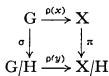
\includegraphics[keepaspectratio]{images/part002_b1d03d5a.jpg}}

于是 \(\pi \circ \rho (x) = \rho (y)\circ \sigma\)，从而

\[
\mathrm{T} _ {x} (\pi) \circ \mathrm{T} _ {e} (\rho (x)) = \mathrm{T} _ {e} (\rho (y)) \circ \mathrm{T} _ {e} (\sigma).
\]

令 \(u \in T_{e}(\mathrm{G/H})\) 满足 \(T_{e}(\rho(y))u = 0\)。存在 \(v \in T_{e}(\mathrm{G})\)，使 \(u = T_{e}(\sigma)v\)。于是 \(T_{x}(\pi)(T_{e}(\rho(x))v) = 0\)，因此 \(T_{e}(\rho(x))v\) 是 Hx 的切向量（Differentiable and Analytic Manifolds, R, 5.10.5），故其具有 \(T_{e}(\rho(x) | H)v'\) 的形式，其中 \(v' \in T_{e}(\mathrm{H})\)。由于 \(T_{e}(\rho(x))\) 是单射，所以 \(v = v'\)，从而 \(v \in T_{e}(\mathrm{H})\)，且 \(u = 0\)。因此 \(T_{e}(\rho(y))\) 是单射。\(T_{e}(\rho(y))\) 的像等于 \(T_{x}(\pi) \circ T_{e}(\rho(x))\) 的像；现在 \(T_{e}(\rho(x))\) 的像在 \(T_{x}(\mathrm{X})\) 中有拓扑补，并且包含 \(T_{x}(\pi)\) 的核。因此可见 \(\rho(y)\) 是浸入，这就完成了 (ii) 的证明。

断言 (iii) 由上述内容和 Differentiable and Analytic Manifolds, R, 5.9.7 得出。

推论。设 G 为李群，H、L 为 G 的正规李子群，且 \(L \subset H\)。则 H/L 是 G/L 的正规李子群，并且从 G/H 到 \((G/L)/(H/L)\) 的典范双射是李群同构。

\subsection{轨道}

命题 14. 设 \(\mathbf{G}\) 为李群，\(\mathbf{X}\) 为解析流形，且 \((g,x)\mapsto gx\) 是 \(\mathbf{G}\) 在 \(\mathbf{X}\) 上的解析左作用律。设 \(x\in \mathbf{X}\)。假设相应的轨道映射 \(\rho (x)\) 是次浸入（如果 \(\mathbf{K}\) 的特征为 0 且 \(\mathbf{X}\) 是有限维的，这总是如此（命题 9 的推论））。令 \(\mathbf{G}_{\mathbf{x}}\) 为稳定子 \(x\) 在 \(\mathbf{G}\) 中的子群。

\begin{enumerate}
\def\labelenumi{(\roman{enumi})}
\item
  \(\mathrm{G}_x\) 是李子群，且 \(\mathrm{T}_e(\mathrm{G}_x) = \mathrm{Ker}\, \mathrm{T}_e(\rho(x))\)。
\item
  齐性空间的典范映射 \(i_x\) 从 \(G / G_x\) 到 \(X\) 是浸入，其像为 \(Gx\)。
\item
  如果进一步轨道 \(\mathbf{G}x\) 是局部闭的且 \(\mathbf{G}\) 的拓扑具有可数基，则 \(\mathbf{G}x\) 是 \(\mathbf{X}\) 的子流形，\(i_x\) 是从流形 \(\mathrm{G} / \mathrm{G}_x\) 到流形 \(\mathbf{G}x\) 的同构，且 \(\mathrm{T}_x(\mathbf{G}x) = \operatorname{Im} \mathrm{T}_e(\rho(x))\)。
\end{enumerate}

\(x\) 在 \(\rho(x)\) 下的逆像是 \(G_x\)。由于 \(\rho(x)\) 是次浸入，\(G_x\) 是子流形，并且对于所有 \(g \in G\)，其切空间 \(J\) 是 \(gG_x = \rho(x)^{-1}(gx)\) 在 \(g\) 处的切空间，且等于 \(\operatorname{Ker} T_g(\rho(x))\)（Differentiable and Analytic Manifolds, R, 5.10.5），从而得到 (i)。令 \(\pi: G \to G/G_x\) 为典范映射。于是 \(i_x \circ \pi = \rho(x)\)。由于 \(G/G_x\) 是 \(G\) 的商流形，这个等式表明 \(i_x\) 是解析的。此外，\(T_g(\rho(x))\) 和 \(T_g(\pi)\) 的核都等于 \(J\)。因此 \(T_{\pi(g)}(i_x)\) 是单射。\(T_{\pi(g)}(i_x)\) 的像等于 \(T_g(\rho(x))\) 的像，因而有拓扑补。这证明了 (ii)。

假设 \(Gx\) 是局部闭的。于是 \(Gx\) 中每一点在 \(Gx\) 中都有一个邻域，它同胚于完备度量空间的闭子空间，因而是 Baire 空间。因此 \(Gx\) 是 Baire 空间（General Topology, Chapter IX, § 5, Proposition 4）。如果 \(G\) 具有可数基，则 \(i_x\) 是从 \(G / G_x\) 到 \(Gx\) 的同胚（General Topology, Chapter IX, § 5）。于是由 (ii) 和 Differentiable and Analytic Manifolds, R, 5.8.3，\(i_x\) 是从流形 \(G / G_x\) 到流形 \(Gx\) 的同构，并且

\[
\mathrm{T} _ {x} (\mathrm{G} x) = \operatorname{Im} \mathrm{T} _ {\pi (e)} (i _ {x}) = \operatorname{Im} \mathrm{T} _ {e} (\rho (x)).
\]

备注。设 G 为有限维李群，X 为 \(C^{r}\) 类流形，且 \((g, x) \mapsto gx\) 是 G 在 X 上的 \(C^{r}\) 类左作用律。则命题 14 仍然成立。唯一需要不同证明的点是 \(G_{x}\) 为李子群这一事实。但若 \(r \neq \omega\)，则 K = R；由于 \(G_{x}\) 显然是闭的，\(G_{x}\) 由§8、定理 2 得出是李子群。

推论。设 G 为拓扑具有可数基的李群，X 为

非空有限维解析流形，且 G 在 X 上有解析左作用律。假设 G 在 X 上传递作用且 K 的特征为 0。则 X 是 G 的李齐性空间。

令 \(x \in X\)。\(x\) 的轨道等于 \(X\)，是闭的，因此可以应用命题 14 (iii)。

\subsection{带算子的向量丛}

设 G 为李群，X 为 \(C^{r}\) 类流形，且 \((g, x) \mapsto gx\) 是 \(C^{r}\) 类的 G 在 X 上的左作用律。设 E 为 \(C^{r}\) 类向量丛，底空间为 X，且 \(\pi: E \to X\) 为 E 到 X 的投影。对于所有 \(x \in X\)，令 \(E_{x}\) 为 E 在 x 处的纤维。令 \((g, u) \mapsto gu\) 为 G 在 E 上的左作用律，使 \(\pi\) 与 G 在 X 和 E 上的作用相容。对于所有 \(g \in G\) 和 \(x \in X\)，将其在 \(E_{x}\) 上的限制 \(u \mapsto gu\) 记为双射 \(\psi_{g,x}\)，它从 \(E_{x}\) 到 \(E_{gx}\)。我们假定，对于所有 \(g \in G\) 和 \(x \in X\)，\(\psi_{g,x}\) 是连续线性的，因而是可赋范空间 \(E_{x}\) 到可赋范空间 \(E_{gx}\) 的同构。

令 \(\phi\) 为自同构 \((g,x)\mapsto (g,gx)\)（定义在流形 \(\mathrm{G}\times \mathrm{X}\) 上）。令 \(p\) 为 \(\mathrm{G}\times \mathrm{X}\) 到 \(\mathbf{X}\) 的典范投影，\(\mathrm{E}'\) 为 \(\mathrm{E}\) 在 \(p\) 下的逆像。令 \(\psi \colon \mathrm{E}'\to \mathrm{E}'\) 为各映射 \(\psi_{g,x}\colon \mathrm{E}_{(g,x)}'\to \mathrm{E}_{(g,gx)}'\) 的和。

定义 4. 如果 \(\psi\) 是向量丛的 \(\phi\)-态射且属于 \(\mathbf{C}^r\) 类，则 \(\mathbf{E}\) 称为向量 \(\mathbf{G}\)-丛，类为 \(\mathbf{C}^r\)。

换言之，E 是 \(C^{r}\) 类向量 G-丛，当且仅当对于所有 \((g_{0}, x_{0}) \in \mathbf{G} \times \mathbf{X}\)，以下条件成立：存在 \((g_{0}, x_{0})\) 在 \(G \times X\) 中的一个开邻域 U，使得，如果 \(E^{\prime} \mid U\)（相应地，\(E^{\prime} \mid \phi(U)\)）借助向量图识别为纤维 M（相应地，N）的平凡向量丛，则映射 \((g, x) \mapsto \psi_{g,x}\) 从 U 到 \(\mathcal{L}(M, N)\) 是 \(C^{r}\) 类的。

映射 \(\psi\) 显然是双射，由上述局部判据可知 \(\psi^{-1}\) 是向量丛的 \(\phi^{-1}\)-态射，因此 \(\psi\) 是向量丛的 \(\phi\)-同构。

以 X 为底空间的平凡向量 G-丛是向量丛 \(X \times F\)（其中 F 是完备可赋范空间），并带有作用律 \((g, (x, f)) \mapsto (gx, f)\) 在 G 的 \(X \times F\) 上的作用。

仍假定定义 4 前的假设和记号，并进一步取 \(\tau\) 为对同构的 \(C^r\) 类向量函子（Differentiable and Analytic Manifolds, R, 7.6.6）。则 \(\tau E\) 是底空间为 \(X\) 的向量丛。对于所有 \(x \in X\)，其纤维 \((\tau E)_x\) 等于 \(\tau (E_x)\)。对于所有可赋范空间 \(N_1, N_2\)，令 \(\operatorname{Isom}(N_1, N_2)\) 表示从 \(N_1\) 到 \(N_2\) 的同构集合。如果 \(g \in G\)，则

\[
\tau (\psi_ {g, x}) \in \operatorname{Isom} ((\tau E) _ {x}, (\tau E) _ {g x}).
\]

\(\tau(\psi_{g,x})\) 定义了左作用律 \((g,u)\mapsto gu\) G 在 \(\tau\) E 上，且 \(\tau\) E 到 X 的典范投影与 G 在 X 和 \(\tau\) E 上的作用相容。

命题 15. 如果 E 是 \(\mathbf{C}^r\) 类向量 G-丛，则 \(\tau \mathbf{E}\) 是 \(\mathbf{C}^r\) 类向量 G-丛。

设 \(g_0, x_0\)、U、M、N 如定义 4 后的段落所述。映射 \((g, x) \mapsto \tau(\psi_{g,x})\) 从 U 到 \(\mathcal{L}(\tau\mathrm{M}, \tau\mathrm{N})\)，是映射 \((g, x) \mapsto \psi_{g,x}\) 从 U 到 \(\mathcal{L}(\mathrm{M}, \mathrm{N})\) 与映射 \(f \mapsto \tau(f)\) 从 \(\operatorname{Isom}(\mathrm{M}, \mathrm{N})\) 到 \(\operatorname{Isom}(\tau\mathrm{M}, \tau\mathrm{N})\) 的复合；这两个映射都是 \(C^r\) 类的，因而复合也如此，从而得到命题。

命题 16. 设 G 为李群，X 为 \(\mathbf{C}^r\) 类流形（\(r \geqslant 2\)），且 \((g, x) \mapsto gx\) 是 G 在 X 上的 \(\mathbf{C}^r\) 类左作用律；因此通过传递结构，G 在 TX 上有一个左作用律。在此作用律下，TX 是 \(\mathbf{C}^{r-1}\) 类向量 G-丛。

令 \(\mathrm{pr}_1\)（相应地，\(\mathrm{pr}_2\)）为从 \(\mathrm{G} \times \mathrm{X}\) 到 \(\mathrm{G}\)（相应地，\(\mathrm{X}\)）的典范投影，并令 \(\mathrm{E}_1\)（相应地，\(\mathrm{E}_2\)）为关于 \(\mathrm{pr}_1\)（相应地，\(\mathrm{pr}_2\)）的 TG（相应地，TX）的逆像。于是向量丛 \(\mathrm{T}(\mathrm{G} \times \mathrm{X})\) 是 \(\mathrm{E}_1\) 和 \(\mathrm{E}_2\) 的直和。令 \(i: \mathrm{E}_2 \to \mathrm{T}(\mathrm{G} \times \mathrm{X})\) 和 \(q: \mathrm{T}(\mathrm{G} \times \mathrm{X}) \to \mathrm{E}_2\) 为由此直和分解定义的典范向量丛态射。令 \(\phi\) 为映射 \((g, x) \mapsto (g, gx)\)，它从 \(\mathrm{G} \times \mathrm{X}\) 到 \(\mathrm{G} \times \mathrm{X}\)。然而，定义 4 中记作 \(\psi\) 的映射（其中取 \(\mathrm{E} = \mathrm{TX}\)）正是 \(q \circ \mathrm{T}(\phi) \circ i\)。但是 \(\mathrm{T}(\phi)\) 是一个 \(\phi\)-态射，并且作为向量丛态射的类为 \(\mathrm{C}^{r-1}\)（Differentiable and Analytic Manifolds, R, 8.1.2）。

推论。若 \(\tau\) 是对同构的 \(\mathbf{C}^r\) 类向量函子，则 \(\tau(\mathrm{TX})\) 是类为 \(\mathbf{C}^{r-1}\) 的向量 G-丛。

这由命题 15 和 16 得出。

注 1. 若 \(\tau\) 是有限维情形下对同构的 \(C^r\) 类向量函子，且 \(E\) 具有有限秩，则 \(\tau E\) 的定义类似，命题 15 仍然成立；只要 \(X\) 是有限维的，命题 16 的推论仍然成立。

例子。取命题 16 的假设和记号，并令 F 为完备可赋范空间。则 \(\mathcal{L}((\mathrm{TX})^p; \mathrm{F})\) 是类为 \(\mathrm{C}^{r-1}\) 的向量 G-丛；如果 K 的特征为零或 X 是有限维的，则 \(\operatorname{Alt}^p(\mathrm{TX}; \mathrm{F})\) 也是如此（参见~Differentiable and Analytic Manifolds, R, 7.7, 7.8）。如果 X 是有限维的，则 \(\bigotimes^p(\mathrm{TX}) \otimes \bigotimes^q(\mathrm{TX})^*\) 是类为 \(\mathrm{C}^{r-1}\) 的向量 G-丛。

命题 17. 设 G 是李群，X 是 G 的左李齐性空间，\(x_0\) 是 X 中的一点，\(G_0\) 是 G 中 \(x_0\) 的稳定子，E 和 E' 是基空间为 X 且类为 \(C^{r}\) 的左向量 G-丛，\(E_0\)（相应地，\(E_0'\)）是 E（相应地，E'）在 \(x_0\) 处的纤维，且 f 是 \(\mathcal{L}(E_0, E_0')\) 中满足 \(f(gu) = g(f(u))\)（对所有 \(u \in E_0\) 和 \(g \in G_0\)）的元素。则存在唯一一个从 E 到 E'、与 G 的作用相容并延拓 f 的态射。这个态射的唯一性是显然的。下面证明其存在性。令 \(g\)、\(g'\) 为 G 中的元素，且 \(u \in E_0\) 满足 \(gu = g'u\)。则 \(g'^{-1}g \in G_0\) 且 \(g'^{-1}gu = u\)，从而 \(g'^{-1}gf(u) = f(u)\)，即 \(gf(u) = g'f(u)\)。因此定义映射 \(\phi\)，其从 E 到 \(E'\)，规定 \(\phi(gu) = gf(u)\)。显然，此映射延拓 \(f\)，并且与 G 的作用相容。我们证明 \(\phi\) 是类为 \(C^r\) 的向量丛态射。令 \(x_1 \in X\)。存在 X 中 \(x_1\) 的开邻域 V 以及 G 的子流形 W，使得映射 \(g \mapsto gx_0\) 是 W 到 V 的同构 \(\theta\)，类为 \(C^r\)。将 V 和 W 缩小后，可设：

\begin{enumerate}
\def\labelenumi{(\arabic{enumi})}
\item
  E \textbar{} V（相应地，E' \textbar{} V）被识别为纤维为 M（相应地，M'）的平凡向量丛；
\item
  若 \(\psi_{g}\)（相应地，\(\psi_{g}^{\prime}\)）表示映射 \(u\mapsto gu\)，其定义域为 \(\mathrm{E}_0\)（相应地，\(\mathrm{E}_0^{\prime}\)），值域为 \(\mathrm{E}_{gx_0}\)（相应地，\(\mathrm{E}_{gx_0}\)），则映射 \(g\mapsto \psi_g\) 和 \(g\mapsto \psi_g^{-1}\)（相应地，\(g\mapsto \psi_g^{\prime}\) 和 \(g\mapsto \psi_g^{\prime -1}\)）从 W 到 \(\mathcal{L}(\mathrm{E}_0,\mathrm{M})\) 和 \(\mathcal{L}(\mathrm{M},\mathrm{E}_0)\)（相应地，\(\mathcal{L}(\mathrm{E}_0',\mathrm{M}')\) 和 \(\mathcal{L}(\mathrm{M}',\mathrm{E}_0'))\)，都是类为 \(C^r\) 的。
\end{enumerate}

对于 \(x \in V\)，令 \(\phi_x: M \to M'\) 为 \(\phi\) 在 \(E_x = M\) 上的限制。于是 \(\phi_x\) 由以下映射复合而成：

\begin{enumerate}
\def\labelenumi{(\arabic{enumi})}
\item
  映射 \((\psi_{\theta^{-1}(x)})^{-1}\)，它从 M 到 \(E_{0}\)；
\item
  从 \(E_{0}\) 到 \(E_{0}'\) 的映射 f；
\item
  映射 \(\psi_{\theta^{-1}(x)}^{\prime}\)，它从 \(\mathbf{E}_0'\) 到 \(\mathbf{M}'\)。
\end{enumerate}

因此可见，映射 \(x \mapsto \phi_x\) 从 V 到 \(\mathcal{L}(\mathbf{M}, \mathbf{M}')\)，且是类为 \(\mathbf{C}^r\) 的。

推论 1. 设 \(\mathrm{E}_0^{\mathbb{G}_0}\) 是 \(\mathrm{E}_0\) 中在 \(\mathbf{G}_0\) 作用下不变的元素所成的集合。对所有 \(u \in \mathrm{E}_0^{\mathbb{G}_0}\)，令 \(\sigma_u\) 为从 X 到 E 的映射，由 \(\sigma_u(gx_0) = gu\)（对所有 \(g \in G\)）定义。

\begin{enumerate}
\def\labelenumi{(\roman{enumi})}
\item
  E 的 G-不变截面†都是类为 \(\mathbf{C}^r\) 的。
\item
  \(u \mapsto \sigma_u\) 是从 \(\mathrm{E}_0^{\mathrm{G}_0}\) 到 E 的 G-不变截面集合的双射。
\end{enumerate}

断言 (ii) 是显然的。为证明 (i)，只需证明每个截面 \(\sigma_{u}\) 都是类为 \(C^r\) 的。令 E' 为基空间 X、纤维为 \(\mathrm{E}_0^{\mathrm{G}_0}\) 的平凡 G-丛。令 \(f\) 为从 \(\mathrm{E}_0^{\mathrm{G}_0}\) 到 \(\mathrm{E}_0\) 的典范嵌入。根据命题 17，存在态射 \(\phi\)，它从 E' 到 E、与 G 的作用相容并延拓 \(f\)。若 \(u \in \mathrm{E}_0^{\mathrm{G}_0}\) 且 \(g \in \mathrm{G}\)，则

\[
\sigma_ {u} (g x _ {0}) = g u = g f (u) = \phi (g u) = \phi ((u, g x _ {0}))
\]

从而有 \(\sigma_u(x) = \phi((u, x))\)，对所有 \(x \in \mathbf{X}\)，这就证明了断言。

*例如，设 G 是有限维实李群，\(G_{0}\) 是 G 的紧李子群，X 是齐性空间 \(G/G_{0}\)。记 X 中 e 的典范像为 \(x_{0}\)。在 \(T_{x_{0}}(X)\) 上存在一个在 \(G_{0}\) 作用下不变的正定对称双线性型（Integration，第 VII 章，第 § 3 节，命题 1）。将上述结果应用于 \((\mathrm{TX})^{*}\otimes(\mathrm{TX})^{*}\)，可见 X 上存在一个在 \(G_{0}\) 作用下不变的解析黎曼度量。

推论 2. 假设 \(G_{0}\) 在 \(E_{0}\) 上平凡作用。令 \(E'\) 为基空间 X、纤维为 \(E_{0}\) 的平凡 G-丛。存在唯一一个从 E 到 \(E'\)、与 G 的作用相容并延拓 \(Id_{E_{0}}\) 的同构。

这立即由命题 17 得出。

注 2. 在本编号中，左作用律处处都可以用右作用律替代。

\subsection{李群的局部定义}

命题 18. 设 \(\mathbf{G}\) 是一个群，\(\mathbf{U}\) 和 \(\mathbf{V}\) 是 \(\mathbf{G}\) 中包含 \(e\) 的两个子集。假设 \(\mathbf{U}\) 具有满足下列条件的解析流形结构：

\begin{enumerate}
\def\labelenumi{(\roman{enumi})}
\item
  \(\mathrm{V} = \mathrm{V}^{-1},\mathrm{V}^2\subset \mathrm{U},\mathrm{V}\) 在 U 中是开集；
\item
  映射 \((x,y)\mapsto xy^{-1}\) 从 \(\mathbf{V}\times \mathbf{V}\) 到 \(\mathbf{U}\)，且是解析的；
\item
  对所有 \(g \in \mathbf{G}\)，存在 \(\mathbf{V}'\)，它是 \(e\) 在 \(\mathbf{V}\) 中的开邻域，使得 \(g\mathbf{V}'g^{-1} \subset \mathbf{U}\)，并且映射 \(x \mapsto gxg^{-1}\) 从 \(\mathbf{V}'\) 到 \(\mathbf{U}\)，且是解析的。
\end{enumerate}

则在 \(\mathbf{G}\) 上存在唯一一个具有下列性质的解析流形结构：

(α) 带此结构的 G 是李群；

(β) V 在 G 中是开集；

\begin{enumerate}
\def\labelenumi{(\Alph{enumi})}
\setcounter{enumi}{24}
\tightlist
\item
  G 和 U 上的流形结构在 V 上诱导出相同的结构。
\end{enumerate}

\begin{enumerate}
\def\labelenumi{(\alph{enumi})}
\item
  令 A 为 V 的开子集，\(v_{0}\) 为 V 中的元素且满足 \(v_{0}A \subset V\)。则 \(v_{0}A\) 是满足 \(v \in V\) 且 \(v_{0}^{-1}v \in A\) 的 v 所成的集合，因而是 V 的开子集（考虑 (ii)）。此外，(ii) 表明，映射 \(v \mapsto v_{0}v\) 从 A 到 \(v_{0}A\)，以及映射 \(v \mapsto v_{0}^{-1}v\) 从 \(v_{0}A\) 到 A，互为解析双射，因而是解析同构。
\item
  取 \(W\)，它是 \(e\) 在 \(V\) 中的开邻域，满足 \(W = W^{-1}\)、\(W^3 \subset V\)，并且存在图表 \((W, \phi, E)\)，它属于流形 \(U\)，其定义域为 \(W\)。对所有 \(g \in G\)，令 \(\phi_g\) 为映射 \(h \mapsto \phi(g^{-1}h)\)，它从 \(gW\) 到 \(E\)。我们证明，图表 \(\phi_g\) 是 \(G\) 的解析相容图表。令 \(g_1, g_2\) 为 \(G\) 中的元素，满足 \(g_1W \cap g_2W \neq \emptyset\)，于是 \(g_2^{-1}g_1\) 和 \(g_1^{-1}g_2\) 属于 \(W^2\)。根据 (a)，\(W \cap g_1^{-1}g_2W\) 是 \(W\) 的开子集，因此
\end{enumerate}

\[
\phi_ {g _ {1}} (g _ {1} \mathrm{W} \cap g _ {2} \mathrm{W}) = \phi (\mathrm{W} \cap g _ {1} ^ {- 1} g _ {2} \mathrm{W})
\]

是 E 的开子集 D。对于 \(d \in \mathbf{D}\)，

\[
\left(\phi_ {g _ {2}} \circ \phi_ {g _ {1}} ^ {- 1}\right) (d) = \phi \left(g _ {2} ^ {- 1} g _ {1} \phi^ {- 1} (d)\right);
\]

由 (a) 可见，\(\phi_{g_2} \circ \phi_{g_1}^{-1}\) 是解析的。

\begin{enumerate}
\def\labelenumi{(\alph{enumi})}
\setcounter{enumi}{2}
\item
  由 (b)，在 \(\mathbf{G}\) 上存在解析流形结构，使 \((\phi_g)_{g\in G}\) 成为 \(\mathbf{G}\) 上的图册。对所有 \(g_0\in \mathbf{G}\)，映射 \(g\mapsto g_0g\)（\(g\in \mathbf{G}\)）保持该图册不变，因而是带此流形结构的 \(\mathbf{G}\) 的自同构。特别地，条件 \((\mathrm{GL}_1)\) 得到满足。
\item
  令 \(v_{0} \in V\)。根据 (ii)，存在 \(A\)，它是 \(e\) 在 \(W\) 中的开邻域，且 \(v_{0}A \subset V\)。这首先证明 \(V\) 是 \(G\) 中的开集。根据 (a)，映射 \(v \mapsto v_{0}v\) 从 \(A\) 到 \(v_{0}A\) 是解析同构，其结构取自 U。根据 (c)，可见 G 和 U 上的流形结构在 \(v_{0}\mathbf{A}\) 上诱导出相同的结构，因而最终在 V 上也相同。
\item
  由 (d)、(ii) 和 (iii)，可见条件 \((\mathrm{GL}_2)\) 和 \((\mathrm{GL}_3)\) 成立。因此 G 是李群。
\item
  如果 G 上的流形结构与 G 的群结构相容，并且 V 是 G 的开子流形，那么 \((\phi_{g})_{g\in G}\) 是 G 上的图册。这就证明了命题的唯一性断言。
\end{enumerate}

命题 19. 设 G 是拓扑群，H 是李群，f 是从群 G 到群 H 的同态。假设存在 G 中 \(e_{G}\) 的一个开邻域、图表 (V, \(\phi\) , E)，它是流形 H 在 \(e_{H}\) 处的图表，以及 E 的一个具有拓扑补空间的闭向量子空间 F，使得 \(f(\mathrm{U}) \subset \mathrm{V}\)，并且 \((\phi \circ f)\mid_U\) 是从 U 到 \(\phi(\mathrm{V}) \cap \mathrm{F}\) 的同胚。则在 G 上存在唯一一个使 f 成为浸入的流形结构；该结构是 H 上流形结构在 f 下的逆像。带此结构的 G 是李群。

由于 G 的平移（相应地，H 的平移）是同胚（相应地，解析同构），f 满足《Differentiable and Analytic Manifolds》R, 5.8.1 中的条件 (R)。于是命题的前两个断言由《Differentiable and Analytic Manifolds》R, 同上处得出。考虑交换图

\[
\begin{array}{c} \mathrm{G} \times \mathrm{G} \xrightarrow {m} \mathrm{G} \\ f \times f \Big \downarrow \qquad \qquad \qquad \qquad \qquad \qquad \qquad \qquad \qquad \Big \downarrow f \\ \mathrm{H} \times \mathrm{H} \xrightarrow {n} \mathrm{H} \end{array}
\]

其中，对于 G（相应地，H）中的 x、y，\(m(x,y)=xy^{-1}\)（相应地，\(n(x,y)=xy^{-1}\)）。则 \(n\circ(f\times f)\) 是解析的，从而 \(f\circ m\) 是解析的；又因为 f 是浸入，所以 m 是解析的。因此 G 是李群。

G 上的李群结构称为 H 上李群结构在 f 下的逆像。

推论。设 G 是拓扑群，N 是 G 的离散正规子群，且 \(\pi\) 是从 G 到 G/N 的典范映射。假设 G/N 上给定了解析流形结构，并且与 G/N 的拓扑群结构相容。则在 G 上存在唯一一个使 \(\pi\) 成为浸入的流形结构；该结构是 G/N 上流形结构在 \(\pi\) 下的逆像。带此结构时，\(\pi\) 是 étale 的，G 是李群，而 G/N 是 G 按 N 作商得到的商李群。

注。设 H 是连通实或复李群，\(\hat{H}\) 是其万有覆盖\(\dagger\)，且 \(\pi\) 是从 \(\hat{H}\) 到 H 的典范映射。当我们把 \(\hat{H}\) 作为李群谈论时，始终指的是 \(\mathbf{H}\) 上的结构在 \(\pi\) 下的逆像结构。

\subsection{李群芽}

定义 5. K 上的李群芽是满足下列条件的系统 (G, e, θ, m)：

\begin{enumerate}
\def\labelenumi{(\roman{enumi})}
\item
  G 是 K 上的解析流形；
\item
  \(e \in G;\)
\item
  \(\theta\) 是从 G 到 G 的解析映射；
\item
  \(m\) 是从开子集 \(\Omega\)（\(\mathbf{G} \times \mathbf{G}\) 的开子集）到 \(\mathbf{G}\) 的解析映射；
\item
  对所有 \(g \in G\)，都有 \((e, g) \in \Omega\)、\((g, e) \in \Omega\) 以及 \(m(e, g) = m(g, e) = g\)；
\end{enumerate}

\[
g \in G, (g, \theta (g)) \in \Omega , (\theta (g), g) \in \Omega , m (g, \theta (g)) = m (\theta (g), g) = e;
\]

\begin{enumerate}
\def\labelenumi{(\roman{enumi})}
\setcounter{enumi}{6}
\tightlist
\item
  若 \(g, h, k\) 是 \(G\) 中满足 \((g, h) \in \Omega\)、\((h, k) \in \Omega\)、\((m(g, h), k) \in \Omega\) 和 \((g, m(h, k)) \in \Omega\) 的元素，则 \(m(m(g, h), k) = m(g, m(h, k))\)。
\end{enumerate}

e 称为李群芽的单位元。我们通常用 gh 代替 \(m(g, h)\)，并且（滥用记号）用 \(g^{-1}\) 代替 \(\theta(g)\)。

李群 G 是取 \(e, \theta, m\) 为显然选择的李群芽。设 G 是李群芽。则 \(ee^{-1} = e\)，即

\[
e ^ {- 1} = e.\tag{8}
\]

对所有 \(g\in G\)

\[
g = e g = ((g ^ {- 1}) ^ {- 1} g ^ {- 1}) g = (g ^ {- 1}) ^ {- 1} (g ^ {- 1} g) = (g ^ {- 1}) ^ {- 1} e,
\]

即

\[
(g ^ {- 1}) ^ {- 1} = g.\tag{9}
\]

G 的一个子集若在映射 \(g \mapsto g^{-1}\) 下不变，就称为对称的。流形 G 取点 e、映射 \(g \mapsto g^{-1}\) 以及映射 \((g, h) \mapsto hg\)，构成称为 G 的对立李群芽的李群芽 G \(^{\nu}\)。

若对于所有 \((g,h)\in \mathbf{G}\times \mathbf{G}\) 中满足 \(gh\) 有定义的元素，\(hg\) 也有定义且等于 \(gh\)，则称李群芽 G 为交换的。

设 \(G\) 是李群芽。由 \((g, h) \in G \times G\) 且 \(gh\) 有定义的元素所成的集合是 \((e, e)\) 的邻域。另一方面，映射 \((g, h) \mapsto gh\) 和 \(g \mapsto g^{-1}\) 是连续的。因此 \((gh)k = g(hk)\)，其中 \(g, h, k\) 充分接近 \(e\)。同样，\((h^{-1}g^{-1})(gh) = h^{-1}(eh) = h^{-1}h = e\)，其中 \(g, h\) 充分接近 \(e\)，于是右乘 \((gh)^{-1}\)，

\begin{enumerate}
\def\labelenumi{(\arabic{enumi})}
\setcounter{enumi}{9}
\tightlist
\item
\end{enumerate}

\((gh)^{-1} = h^{-1}g^{-1}\)，其中 \(g,h\) 充分接近 \(e\)。

命题 20. 设 G 是李群芽且 \(g \in G\)。存在 e 的开邻域 U 和 g 的开邻域 V，具有下列性质：

\begin{enumerate}
\def\labelenumi{(\alph{enumi})}
\item
  对所有 \(u \in U\)，ug 有定义；
\item
  \(vg^{-1}\) 对所有 \(v \in V\) 都有定义；
\item
  映射 \(u \mapsto ug\)、\(v \mapsto vg^{-1}\) 彼此互为从 U 到 V 及从 V 到 U 的解析同构。
\end{enumerate}

  由于乘积的定义域是 \(\mathbf{G} \times \mathbf{G}\) 中的开集，存在 \(e\) 的开邻域 U 和 \(g\) 的开邻域 V，具有性质 (a) 和 (b)。令 \(\eta(u) = ug\)（\(u \in \mathrm{U}\)），\(\eta'(v) = vg^{-1}\)（\(v \in \mathrm{V}\)）。缩小 U 和 V，可设 \((ug)g^{-1} = u\) 以及 \((vg^{-1})g = v\)，其中 \(u \in \mathrm{U}\) 和 \(v \in \mathrm{V}\)。于是 \(\eta\) 和 \(\eta'\) 是单射。再缩小 U，可设 \(\eta(\mathrm{U}) \subset \mathrm{V}\)。于是 \(\eta'(\mathrm{V}) \supset \mathrm{U}\)，且 \(\eta(\mathrm{U})\) 是 \(\eta'\) 下 U 的逆像，因而是 V 中 \(g\) 的开邻域。将 V 替换为 \(\eta(\mathrm{U})\)，最终得到 \(\eta\) 和 \(\eta'\) 是解析的互逆双射。

设 \(G_{1}, G_{2}\) 是两个李群芽，单位元分别为 \(e_{1}, e_{2}\)。从 \(G_{1}\) 到 \(G_{2}\) 的映射 f 若满足下列条件，就称为态射：

\begin{enumerate}
\def\labelenumi{(\roman{enumi})}
\item
  \(f\) 是解析的；
\item
  \(f(e_{1}) = e_{2};\)
\item
  若 \(g, h\) 是 \(\mathbf{G}_1\) 中满足 \(gh\) 有定义的元素，则 \(f(g)f(h)\) 有定义且等于 \(f(gh)\)。
\end{enumerate}

令 \(g \in G_1\)。由于 \(gg^{-1}\) 有定义且等于 \(e_1, f(g)f(g^{-1})\) 有定义并等于 \(e_2\)，从而

\[
f (g) ^ {- 1} = f (g) ^ {- 1} \left(f (g) f \left(g ^ {- 1}\right)\right) = \left(f (g) ^ {- 1} f (g)\right) f \left(g ^ {- 1}\right)
\]

即

\[
f (g) ^ {- 1} = f (g ^ {- 1}).\tag{11}
\]

两个态射的复合仍是态射。

若 \(f: \mathbf{G}_1 \to \mathbf{G}_2\) 和 \(f': \mathbf{G}_2 \to \mathbf{G}_1\) 互为逆态射，则它们是同构（特别使用公式 (11)）。

设 \(G_{1}\)、\(G_{2}\) 是两个李群芽，f 是从 \(G_{1}\) 到 \(G_{2}\) 的映射，满足上述条件 (ii) 和 (iii)，并且在 \(e_{1}\) 的一个开邻域内解析。利用命题 20，可仿照命题 4 证明 f 是态射。

设 \((\mathbf{G}, e, \theta, m)\) 是李群芽，\(\Omega\) 是 \(m\) 的定义集。令 \(\mathbf{H}\) 为 \(\mathbf{G}\) 的子流形，它包含 \(e\) 且在 \(\theta\) 下稳定。假设集合 \(\Omega_1\)（由 \((x, y) \in \Omega \cap (\mathbf{H} \times \mathbf{H})\) 中满足 \(m(x, y) \in \mathbf{H}\) 的元素所成）在 \(\mathbf{H} \times \mathbf{H}\) 中是开集。则 \((\mathbf{H}, e, \theta | \mathbf{H}, m | \Omega_1)\) 是李群芽。这样的李群芽称为 \(\mathbf{G}\) 的李子群芽。将 \(\mathbf{H}\) 典范嵌入 \(\mathbf{G}\) 的映射是态射。若 \(f: \mathbf{L} \to \mathbf{G}\) 是李群芽的态射且 \(f(\mathbf{L}) \subset \mathbf{H}\)，则 \(f: \mathbf{L} \to \mathbf{H}\) 是李群芽的态射。

设 K 的特征为 0。若将 H 是 G 的子流形这一假设替换为 H 是 G 的拟子流形这一假设，上述段落的结果仍然成立（参见《Differentiable and Analytic Manifolds》R, 5.8.5）。此时 H 称为 G 的李拟子群芽。

若 G 是单位元为 e 的李群芽，则 G 中 e 的每个对称开邻域都是 G 的李子群芽。（当 G 是李群时尤其如此。）设 H 是 G 的李子群芽；若 H 是 G 中 e 的邻域，则根据命题 20，H 在 G 中是开集。

有限个李群芽的乘积李群芽按显然的方式定义。

命题 21. 设 G、H 是两个李群芽，\(\phi\) 是从 G 到 H 的态射。下列条件等价：

\begin{enumerate}
\def\labelenumi{(\roman{enumi})}
\item
  \(\phi\) 在 \(e\) 处是 étale 的；
\item
  存在 G、H 的开李子群芽 G'、H'，使得 \(\phi|G'\) 是从 G' 到 H' 的同构。
\end{enumerate}

蕴含 \(\langle \mathrm{ii}\rangle \Rightarrow \langle \mathrm{i}\rangle\) 是显然的。假设 \(\phi\) 在 \(e\) 处是 étale 的。存在开李子群芽 \(\mathbf{G}_1\)，它是 \(\mathbf{G}\) 的开李子群芽，使得 \(\phi (\mathbf{G}_1)\) 在 \(\mathbf{H}\) 中是开集，并且 \(\phi |\mathbf{G}_1\) 是流形 \(\mathbf{G}_1\) 到流形 \(\phi (\mathbf{G}_1)\) 的同构。于是存在开李子群芽 \(\mathbf{G}'\)，它是 \(\mathbf{G}_1\) 的开李子群芽，使得 \(\mathbf{G}\) 中 \(\mathbf{G}'\) 的两个元素的乘积总有定义且属于 \(\mathbf{G}_1\)。若 \(g, g'\) 是 \(\mathbf{G}'\) 中满足 \(\mathrm{gg}^{\prime}\in \mathrm{G}'\) 的元素，则 \(\phi (g)\phi (g') = \phi (gg')\in \phi (\mathbf{G}')\)；若 \(g, g'\) 是 \(\mathbf{G}'\) 中满足 \(gg^{\prime}\in G_1 - G'\) 的元素，则

\[
\phi (g) \phi (g ^ {\prime}) = \phi (g g ^ {\prime}) \in \phi (\mathrm{G} _ {1}) - \phi (\mathrm{G} ^ {\prime}).
\]

因此 \(\phi |G^{\prime}\) 是李群芽 \(G^{\prime}\) 到 H 的开李子群芽 \(\phi (G^{\prime})\) 的同构。

若命题 21 的条件成立，则称 G 和 H 局部同构。

命题 22. 设 H 是李群，U 是 H 的李子群芽，N 是由 \(g \in \mathrm{H}\) 所成的集合，其中 U 与 \(g\mathrm{Ug}^{-1}\) 在 \(e\) 处具有相同的芽（《General Topology》，第 I 章，第 § 6 节，编号 10）。则 \(N\) 是包含 U 的 H 的子群。在 \(\mathbb{N}\) 上存在唯一一个具有下列性质的解析流形结构：

\begin{enumerate}
\def\labelenumi{(\roman{enumi})}
\item
  带此结构的 N 是李群；
\item
  U 是 N 的开子流形；
\item
  从 \(\mathbf{N}\) 到 \(\mathbf{H}\) 的典范嵌入是浸入。
\end{enumerate}

显然，\(\mathbf{N}\) 是 \(\mathbf{H}\) 的子群。若 \(g \in \mathbf{U}\)，则 \(ge \in \mathbf{U}\) 且 \(geg^{-1} \in \mathbf{U}\)，因而 \(gu \in \mathbf{U}\) 且 \(gug^{-1} \in \mathbf{U}\)，其中 \(u\) 充分接近 \(e\)（在 \(\mathbf{U}\) 中），所以 \(g\mathrm{U}g^{-1}\) 在 \(e\) 处的芽包含于 \(\mathbf{U}\) 的芽；交换 \(g\) 和 \(g^{-1}\) 后，可见 \(g\mathrm{U}g^{-1}\) 和 \(\mathbf{U}\) 在 \(e\) 处的芽相等。因此 \(\mathbf{U} \subset \mathbf{N}\)。

令 \(\mathbf{V}\) 为 \(e\) 在 \(\mathbf{U}\) 中的开邻域，使 \(\mathrm{V} = \mathrm{V}^{-1}\)、\(\mathrm{V}^2 \subset \mathrm{U}\)。第 9 号命题 18 的条件 (i)、(ii)、(iii)（其中以 \(\mathrm{G}\) 替换为 \(\mathrm{N}\)）成立。于是，在 \(\mathbf{N}\) 上存在解析流形结构，具有下列性质：\((\alpha)\) 带此结构的 \(\mathbf{N}\) 是李群；\((\beta)\) \(\mathbf{V}\) 在 \(\mathbf{N}\) 中是开集；\((\gamma)\) \(\mathbf{N}\) 和 \(\mathbf{U}\) 上的流形结构在 \(\mathbf{V}\) 上诱导出相同的结构。由于 \(\mathbf{V}\) 是 \(\mathbf{H}\) 的子流形，从 \(\mathbf{N}\) 到 \(\mathbf{H}\) 的典范嵌入在 \(e\) 处是浸入，因而在 \(\mathbf{N}\) 的每一点处都是浸入。令 \(u \in \mathbf{U}\)。存在 \(V'\)，它是 e 在 V 中的开邻域，使映射 \(v \mapsto vu\) 在 \(V'\) 上是解析同构，映到 U 中 u 的一个开邻域（命题 20），同时也映到 N 中 u 的一个开邻域。因此 U 在 N 中是开集，并且 U 的恒等映射关于 U 上给定的流形结构和 N 上的开子流形结构是同构；换言之，U 是 N 的开子流形。

最后，考虑 N 上具有命题条件 (i)、(ii) 的解析流形结构，并令 \(N^{*}\) 为由此得到的李群。于是从 N 到 \(N^{*}\) 的恒等映射在 e 处是 étale 的，因而是李群同构。这证明了命题的唯一性断言。

设 H 是李群，U 是 H 的李拟子群芽，N 是由 \(g \in H\) 所成的集合，其中 U 与 \(gUg^{-1}\) 在 e 处具有相同芽。若 K 的特征为 0，则在 G 上存在唯一一个具有命题 22 的条件 (i)、(ii) 的流形结构。证明与命题 22 相同。

推论。沿用命题 22 的记号，令 G 为 H 中由 U 生成的子群。则 G 是 N 的开子群。在 G 上存在唯一一个李群结构，使 U 是 G 的开子流形，且从 G 到 H 的典范嵌入是浸入。

注。沿用命题 22 及其推论的记号，假设 K 的特征为 0，H 是有限维的，且 U 上的拓扑具有可数基。即使有这些假设，也可能 G 在 H 中不是闭集（习题 3）。但是，若 G 是闭集，则 G 是 H 的李子群。因为映射 \((g,h)\mapsto gh\) 是 G 在 H 上的解析左作用律，e 的轨道是 G。于是我们的断言由命题 2 (iv) 和命题 14 (iii) 得出。

\subsection{作用律片段}

设 \((G, e, \theta, m)\) 是李群芽，X 是类为 \(C^r\) 的流形。

定义 6. 类为 \(\mathbf{C}^r\) 的 \(\mathbf{G}\) 在 \(\mathbf{X}\) 上的左作用律片段，是一个映射 \(\psi\)，定义在 \(\Omega\) 上；该开集位于 \(\mathbf{G} \times \mathbf{X}\) 中，包含 \(\{e\} \times \mathbf{X}\)，且该映射取值于 \(\mathbf{X}\)，并具有下列性质：

\begin{enumerate}
\def\labelenumi{(\roman{enumi})}
\item
  \(\psi\) 是类为 \(C^{r}\) 的；
\item
  对所有 \(x \in X\)，\(\psi(e, x) = x\)；
\item
  存在一个邻域 \(\Omega_1\)，它是 \(\{e\} \times \{e\} \times \mathbf{X}\) 在 \(\mathbf{G} \times \mathbf{G} \times \mathbf{X}\) 中的邻域，使得对于 \((g, g', x) \in \Omega_1\)，\(m(g, g')\)、\(\psi(m(g, g'), x)\) 和 \(\psi(g, \psi(g', x))\) 都有定义，并且 \(\psi(g, \psi(g', x)) = \psi(m(g, g'), x)\)。
\end{enumerate}

类为 \(\mathbf{C}^r\) 的右作用律片段类似定义。

我们通常用 \(gx\) 代替 \(\psi(g, x)\)。

设 \(G'\) 是 G 的李子群芽，\(X'\) 是 X 的子流形。假设集合 \(\Omega'\)，即由 \((g,x)\in \Omega \cap (\mathrm{G}'\times \mathrm{X}')\) 中满足 \(\psi (g,x)\in \mathrm{X}'\) 的元素组成的集合，在 \(\mathrm{G}'\times \mathrm{X}'\) 中是开集（若 \(\mathbf{X}'\) 在 \(\mathbf{X}\) 中是开集，则这一条件总能满足）。则 \(\psi |\Omega '\) 是类为 \(\mathrm{C}^r\) 的左作用律片段，作用于 \(\mathrm{G}'\) 和 \(\mathrm{X}'\)，称为由 \(\psi\) 限制到 \(\mathrm{G}'\) 和 \(\mathrm{X}'\) 所得到的作用律片段。

命题 23. 设 \((\mathbf{G}, e, \theta, m)\) 是李群芽，\(\mathbf{X}\) 是类为 \(\mathbf{C}^r\) 的流形，\(x_0\) 是 \(\mathbf{X}\) 中的一点，\(\Omega\) 是 \((e, x_0)\) 在 \(\mathbf{G} \times \mathbf{X}\) 中的开邻域，\(\psi\) 是从 \(\Omega\) 到 \(\mathbf{X}\) 的映射，具有下列性质：

\begin{enumerate}
\def\labelenumi{(\roman{enumi})}
\item
  \(\psi\) 是类为 \(C^{r}\) 的；
\item
  \(\psi(e, x)\) 在 x 充分接近 \(x_{0}\) 时等于 x；
\item
  \(\psi(m(g, g'), x) = \psi(g, \psi(g', x))\)，其中 \((g, g', x)\) 充分接近 \((e, e, x_0)\)。
\end{enumerate}

则存在开邻域 \(\mathbf{X}'\)，它是 \(x_0\) 在 \(\mathbf{X}\) 中的开邻域，以及开子集 \(\Omega'\)，它是 \(\Omega \cap (\mathrm{G} \times \mathrm{X}')\) 的开子集，使得 \(\psi|\Omega'\) 是类为 \(\mathbf{C}^r\) 的左作用律片段，作用于 \(\mathbf{G}\) 和 \(\mathbf{X}'\)。

存在开邻域 \(\mathbf{X}'\)，它是 \(x_0\) 在 \(\mathbf{X}\) 中的开邻域，以及开邻域 \(\mathbf{G}'\)，它是 \(e\) 在 \(\mathbf{G}\) 中的开邻域，使得 \(\psi(e, x) = x\) 对所有 \(x \in \mathbf{X}'\) 成立，并且

\[
\psi (g, \psi (g ^ {\prime}, x)) = \psi (m (g, g ^ {\prime}), x)
\]

对于 \((g, g', x) \in \mathrm{G}' \times \mathrm{G}' \times \mathrm{X}'\)。令 \(\Omega'\) 为由 \((g, x) \in \Omega \cap (\mathrm{G}' \times \mathrm{X}')\) 中满足 \(\psi(g, x) \in \mathrm{X}'\) 的元素所成的集合。于是 \(\Omega'\) 在 \(\mathrm{G} \times \mathrm{X}'\) 中是开集，并且 \(\mathrm{X}'\)、\(\Omega'\) 具有命题中的性质。

引理 3. 设 \(\mathbf{X}\) 是正规空间，\((\mathbf{X}_i)_{i\in I}\) 是 \(\mathbf{X}\) 的局部有限开覆盖。对所有 \((i,j)\in I\times I\) 以及所有 \(x\in \mathbf{X}_i\cap \mathbf{X}_j\)，令 \(\mathrm{V}_{ij}(x)\) 为一个 \(x\) 的邻域，包含于 \(\mathbf{X}_i\cap \mathbf{X}_j\)。于是可以为每个 \(x\in X\) 关联 \(\mathrm{V}(x)\)，它是 \(x\) 的一个邻域，使下列条件成立：

\begin{enumerate}
\def\labelenumi{(\alph{enumi})}
\item
  若 \(x \in \mathbf{X}_i \cap \mathbf{X}_j\)，则 \(\mathrm{V}(x) \subset \mathrm{V}_{ij}(x)\)；
\item
  若 \(\mathrm{V}(x)\) 与 \(\mathrm{V}(y)\) 相交，则存在 \(i\in \mathbf{I}\)，使 \(\mathrm{V}(x)\cup \mathrm{V}(y)\subset \mathrm{X}_i\)
\end{enumerate}

存在开覆盖 \(\langle \mathrm{X}_i\rangle_{i\in I}\)，它覆盖 \(\mathbf{X}\)，使得 \(\overline{\mathbf{X}}_i' \subset \mathbf{X}_i\) 对所有 \(i \in I\) 成立（《General Topology》，第 IX 章，第 § 4 节，定理 3）。令 \(x \in \mathbf{X}\)。令 \(\mathrm{V}_1(x)\) 为 \(\mathrm{V}_{ij}(x)\) 与 \(\mathbf{X}_k'\) 的交集，其中这些集合包含 \(x\)；这是 \(x\) 的开邻域。令 \(\mathrm{V}_2(x)\) 为 \(x\) 的一个邻域，包含于 \(\mathrm{V}_1(x)\) 且只与有限个 \(\mathbf{X}_i\) 相交。于是 \(\mathrm{V}_2(x)\) 只与有限个 \(\overline{\mathbf{X}}_i'\) 相交，因此下式中的集合

\[
\mathrm{V} (x) = \mathrm{V} _ {2} (x) \cap \bigcap_ {i \in I, x \notin \overline {{\mathrm{X}}} _ {i} ^ {\prime}} (\mathrm{X} - \overline {{\mathrm{X}}} _ {i} ^ {\prime})
\]

是 \(x\) 的邻域。若 \(x \in \mathrm{X}_1 \cap \mathrm{X}_j\)，则 \(\mathrm{V}_1(x) \subset \mathrm{X}_1 \cap \mathrm{X}_j\)，从而 \(\mathrm{V}(x) \subset \mathrm{X}_1 \cap \mathrm{X}_j\)。令 \(x, y\) 属于 \(\mathrm{X}\)，并假设 \(\mathrm{V}(x)\) 与 \(\mathrm{V}(y)\) 相交。存在 \(i \in I\)，使 \(x \in \mathrm{X}_i'\)。于是 \(\mathrm{V}_1(x) \subset \mathrm{X}_i'\)，从而 \(\mathrm{V}(x) \subset \mathrm{X}_i'\)，并且 \(\mathrm{V}(y) \cap \overline{\mathrm{X}_i'} \neq 0\)。于是 \(y \in \overline{\mathrm{X}_i'}\)，根据 \(\mathrm{V}(y)\) 的定义，从而 \(y \in \mathrm{X}_i\) 且 \(\mathrm{V}(y) \subset \mathrm{X}_i\)。因此 \(\mathrm{X}_i\) 包含 \(\mathrm{V}(x)\) 和 \(\mathrm{V}(y)\)。

命题 24. 设 G 是李群芽，X 是类为 \(C^{r}\) 的流形，且 (X \(_{i}\) ) \(_{i \in I}\) 是 X 的局部有限开覆盖。对所有 i ∈ I，令 \(\psi_{i}\) 为 G 上类为 \(C^{r}\) 的左作用律片段，作用于 X \(_{i}\)。假设 X 的底层拓扑空间是正规空间，并且对于所有 (i, j) ∈ I × I 以及所有 x ∈ X \(_{i}\) ∩ X \(_{j}\)，\(\psi_{i}\) 与 \(\psi_{j}\) 在 (e, x) 的一个邻域上重合。存在左作用律片段 \(\psi\)，它是 G 在 X 上的类为 \(C^{r}\) 的左作用律片段，使得对所有 i ∈ I 以及所有 x ∈ X \(_{i}\)，\(\psi_{i}\) 与 \(\psi\) 在 (e, x) 的一个邻域上重合。

对所有 \((i,j)\in \mathrm{I}\times \mathrm{I}\) 以及所有 \(x\in \mathrm{X}_i\cap \mathrm{X}_j\)，选取 \(\mathrm{V}_{ij}(x)\)，它是 \(x\) 的开邻域且包含于 \(\mathrm{X}_i\cap \mathrm{X}_j\)，使 \(\psi_i\) 和 \(\psi_j\) 在 \(\{e\} \times \mathrm{V}_{ij}(x)\) 在 \(\mathrm{G}\times \mathrm{X}\) 中的一个邻域上有定义且相等。对所有 \(x\in \mathrm{X}\)，选取 \(\mathrm{V}(x)\)，它是 \(x\) 在 \(\mathrm{X}\) 中的开邻域，使引理 3 的条件 (a) 和 (b) 得到满足。令 \(\mathbf{I}_x\) 为由 \(i\in \mathrm{I}\) 且 \(x\in \mathrm{X}_i\) 的 i 所成的集合。这是有限集。令 \(\mathrm{U}_x\) 为由 \((g,y)\in \mathrm{G}\times \mathrm{V}(x)\) 所成的集合，其中 \(\psi_i\)（\(i\in \mathrm{I}_x\)）在 \((g,y)\) 的一个邻域上有定义且彼此重合。于是 \(\mathrm{U}_x\) 是开集且 \((e,x)\in \mathrm{U}_x\)。对于 \(\psi_i\)（\(i\in \mathrm{I}_x\)），它们在 \(\mathrm{U}_x\) 上都有相同的限制。令 \(x,y\) 属于 \(\mathrm{X}\)。若 \(\mathrm{U}_x\) 与 \(\mathrm{U}_y\) 相交，则 \(\mathrm{V}(x)\) 与 \(\mathrm{V}(y)\) 相交，因而存在 \(i\in \mathrm{I}\) 使

\[
\mathrm{V} (x) \cup \mathrm{V} (y) \subset \mathrm{X} _ {i}.
\]

于是 \(i \in \mathrm{I}_x, i \in \mathrm{I}_y, \psi_i | \mathrm{U}_x = \psi_x, \psi_i | \mathrm{U}_y = \psi_y\)，从而

\[
\psi_ {x} | (\mathrm{U} _ {x} \cap \mathrm{U} _ {y}) = \psi_ {y} | (\mathrm{U} _ {x} \cap \mathrm{U} _ {y}).
\]

因此，\(\psi_x\) 定义了映射 \(\psi\)，它从 \(\mathbf{U} = \bigcup_{x\in \mathbf{X}}\mathbf{U}_x\) 到 \(\mathbf{X}\)，且 \(\mathbf{U}\) 是 \(\{e\} \times \mathbf{X}\) 在 \(\mathbf{G}\times \mathbf{X}\) 中的开邻域。显然，\(\psi\) 是类为 \(C^r\) 的，且 \(\psi (e,x) = x\) 对所有 \(x\in \mathbf{X}\) 成立。对于所有 \(i\in \mathbf{I}\) 及所有 \(x\in \mathrm{X}_i\)，\(\psi\) 与 \(\psi_x\) 及 \(\psi_i\) 在 \((e,x)\) 的一个邻域上重合，于是 \(\psi\) 满足定义 6 的条件 (iii)。

\section{李群的切向量群}

\subsection{切向复合律}

设 X 和 Y 是类为 \(C^{r}\) 的流形。我们知道（《Differentiable and Analytic Manifolds》R, 8.1.4），\(X \times Y\) 是类为 \(C^{r}\) 的流形，并且映射 \((\mathrm{T}(\mathrm{pr}_{1}), \mathrm{T}(\mathrm{pr}_{2}))\)，即到典范投影的切映射之积，是类为 \(C^{r-1}\) 的同构，从 \(\mathrm{T}(\mathrm{X} \times \mathrm{Y})\) 到 \(\mathrm{T}(\mathrm{X}) \times \mathrm{T}(\mathrm{Y})\)。这个同构与基空间为 \(X \times Y\) 的向量丛结构相容，并允许我们将 \(\mathrm{T}(\mathrm{X} \times \mathrm{Y})\) 识别为 \(\mathrm{T}(\mathrm{X}) \times \mathrm{T}(\mathrm{Y})\)。令 \(a \in \mathbf{X}, b \in \mathbf{Y}, u \in \mathrm{T}_a(\mathbf{X}), v \in \mathrm{T}_b(\mathbf{Y})\)；上述识别使我们可以把 \((u, v)\) 视为 \(\mathrm{T}_{(a,b)}(\mathbf{X} \times \mathbf{Y})\) 中的元素；于是

\[
(u, v) = (u, 0) + (0, v)
\]

并且 \((u,0)\)（相应地，\((0,v))\) 是 \(u\)（相应地，\(v\)）在浸入 \(x\mapsto (x,b)\)（相应地，\(y\mapsto (a,y)\)）的切映射下的像，该浸入将 X（相应地，Y）映入 \(\mathbf{X}\times \mathbf{Y}\)。需要精确说明时，我们将 \(0_{a}\) 记为 \(\mathrm{T}_a(X)\) 的零元素。

现在设 X、Y、Z 是类为 \(C^{r}\) 的流形，且 f 是类为 \(C^{r}\) 的从 \(X \times Y\) 到 Z 的映射。利用上述识别，切映射是类为 \(C^{r-1}\) 的从 \(T(X) \times T(Y)\) 到 \(T(Z)\) 的映射。对于 \(u \in T_{a}(X)\) 和 \(v \in T_{b}(Y)\)，

\begin{enumerate}
\def\labelenumi{(\arabic{enumi})}
\tightlist
\item
\end{enumerate}

\[
\mathrm{T} (f) (u, v) = \mathrm{T} (f) (u, 0 _ {b}) + \mathrm{T} (f) (0 _ {a}, v),
\]

\[
\mathrm{T} (f) \left(0 _ {a}, 0 _ {b}\right) = 0 _ {f (a, b)}.\tag{2}
\]

另一方面，映射 \(y \mapsto f(a, y)\) 是浸入 \(y \mapsto (a, y)\) 与 f 的复合；因此

\begin{enumerate}
\def\labelenumi{(\arabic{enumi})}
\setcounter{enumi}{2}
\item
  \(\mathrm{T}(f)(0,v)\) 是 v 在切映射 \(y\mapsto f(a,y)\) 下的像。同样，
\item
  \(\mathbf{T}(f)(u,0)\) 是 \(u\) 在切映射 \(x\mapsto f(x,b)\) 下的像。
\end{enumerate}

若映射 \(f\) 从 \(\mathbf{X} \times \mathbf{Y}\) 到 \(\mathbf{Z}\) 记作 \((x, y) \mapsto xy\)，则常用 \(uv\) 表示元素 \(T(f)(u, v)\)，其中 \(u \in T(\mathbf{X})\)、\(v \in T(\mathbf{Y})\)。

设 X 是类为 \(C^{r}\) 的流形，且有复合律 \(m: X \times X \to X\)，其类为 \(C^{r}\)。则 \(T(m)\) 是类为 \(C^{r-1}\) 的 \(T(X)\) 上的复合律。它称为与 m 相切的复合律。从 \(T(X)\) 投影到 X 的典范投影 p 与复合律 m 和 \(T(m)\) 相容；换言之，

\[
p \circ \mathrm{T} (m) = m \circ (p \times p).\tag{5}
\]

由 (2) 可得

\[
\mathrm{T} (m) \left(0 _ {x}, 0 _ {y}\right) = 0 _ {m (x, y)}\tag{6}
\]

对所有 \(x, y\) 属于 \(\mathbf{X}\)，换言之，零截面 \(x \mapsto 0_x\)（属于 \(\mathrm{T}(\mathbf{X})\)）与律 \(m\) 和 \(\mathrm{T}(m)\) 相容。

命题 1. 设 X 是类为 \(\mathbf{C}^r\) 的流形，且 \(m\) 是 X 上类为 \(\mathbf{C}^r\) 的复合律。若 \(m\) 是结合的（相应地，交换的），则 \(\mathrm{T}(m)\) 是结合的（相应地，交换的）。

若 \(m\) 是结合的，则 \(m \circ (m \times \mathrm{Id}_{\mathbf{x}}) = m \circ (\mathrm{Id}_{\mathbf{x}} \times m)\)，从而

\[
\mathrm{T} (m) \circ (\mathrm{T} (m) \times \mathrm{Id} _ {\mathrm{T} (\mathbf {X})}) = \mathrm{T} (m) \circ (\mathrm{Id} _ {\mathrm{T} (\mathbf {X})} \times \mathrm{T} (m))
\]

从而 \(\mathrm{T}(m)\) 是结合的。令 \(s\) 为映射 \((x,y)\mapsto (y,x)\)，它从 \(\mathbf{X}\times \mathbf{X}\) 到 \(\mathbf{X}\times \mathbf{X}\)。若 \(m\) 是交换的，则 \(m\circ s = m\)，从而

\[
\mathrm{T} (m) \circ \mathrm{T} (s) = \mathrm{T} (m).
\]

但是，\(\mathrm{T}(s)\) 是映射 \((u,v)\mapsto (v,u)\)，它从 \(\mathrm{T}(\mathbf{X})\times \mathrm{T}(\mathbf{X})\) 到 \(\mathrm{T}(\mathbf{X})\times \mathrm{T}(\mathbf{X})\)。因此 \(\mathrm{T}(m)\) 是交换的。

命题 2. 设 X 是类为 \(\mathbf{C}^r\) 的流形，\(m\) 是 X 上类为 \(\mathbf{C}^r\) 的复合律，\(e\) 是 \(m\) 的单位元。

\begin{enumerate}
\def\labelenumi{(\roman{enumi})}
\item
  向量 \(0_{e}\) 是 \(\mathbf{T}(m)\) 的单位元。
\item
  \(\mathrm{T}_{e}(\mathbf{X})\) 在 \(\mathrm{T}(m)\) 下稳定，并且 \(\mathrm{T}_{e}(\mathbf{X})\) 上由 \(\mathrm{T}(m)\) 诱导的复合律是 \(\mathrm{T}_{e}(\mathbf{X})\) 上的向量空间加法。
\item
  令 U 为 X 的开子集，\(\alpha\) 为从 U 到 X 的类为 \(C^{r}\) 的映射，使得对所有 \(x \in U\)，\(\alpha(x)\) 是 x 在 m 下的逆元。则对所有 \(u \in T(U)\)，\(T(\alpha)u\) 是 u 在 \(T(m)\) 下的逆元。
\end{enumerate}

性质 (3) 和 (4) 表明，\(\mathrm{T}(m)(0_e,u) = \mathrm{T}(m)(u,0_e) = u\) 对所有 \(u\in \mathrm{T}(\mathbf{X})\) 成立，从而得到 (i)。对于 \(u,v\)，它们属于 \(\mathrm{T}_e(\mathbf{X})\)，

\[
\mathrm{T} (m) (u, v) = \mathrm{T} (m) (u, 0 _ {e}) + \mathrm{T} (m) (0 _ {e}, v) = u + v,
\]

从而得到 (ii)。最后，关系 \(m(x, \alpha(x)) = m(\alpha(x), x) = e\) 对所有 \(x \in \mathbf{U}\) 成立，这意味着

\[
\mathrm{T} (m) (u, \mathrm{T} (\alpha) (u)) = \mathrm{T} (m) (\mathrm{T} (\alpha) u, u) = 0 _ {e}
\]

对所有 \(u \in \mathrm{T}(\mathrm{U})\) 成立，从而得到 (iii)。

命题 3. 设 \(\mathbf{X}_1, \mathbf{X}_2, \ldots, \mathbf{X}_p\)、Y 是类为 \(\mathbf{C}^r\) 的流形，i 是 \([1, p]\) 中的整数，\(m_t\)（相应地，n）是类为 \(\mathbf{C}^r\) 的复合律，作用于 \(\mathbf{X}_t\)（相应地，Y），且 u 是类为 \(\mathbf{C}^r\) 的从 \(\mathbf{X}_1 \times \mathbf{X}_2 \times \dots \times \mathbf{X}_p\) 到 Y 的映射。若 u 关于下标为 i 的变量满足分配律，则 T(u) 关于下标为 i 的变量也满足分配律。

证明类似于命题 1 的证明。

\subsection{李群的切向量群}

命题 4. 设 G 是李群。则 T(G) 配备与 G 的乘法相切的复合律后是李群。T(G) 的单位元是向量 \(0_{e}\)。

这由命题 1 和命题 2 得出。

命题 5. 设 G、H 是李群，f 是从 G 到 H 的态射。则 T(f) 是从李群 T(G) 到李群 T(H) 的态射。

我们知道 \(\mathrm{T}(f)\) 是解析的。另一方面，令 m（相应地，n）表示 G（相应地，H）上的乘法。则 \(f \circ m = n \circ (f \times f)\)，从而

\[
\mathrm{T} (f) \circ \mathrm{T} (m) = \mathrm{T} (n) \circ (\mathrm{T} (f) \times \mathrm{T} (f)),
\]

这表达了 \(T(f)\) 是群同态这一事实。

推论。设 \(G_{1},\ldots,G_{n}\) 是李群。从流形 \(\mathrm{T}(\mathrm{G}_{1}\times\cdots\times\mathrm{G}_{n})\) 到流形 \(\mathrm{T}(\mathrm{G}_{1})\times\cdots\times\mathrm{T}(\mathrm{G}_{n})\) 的典范同构是李群同构。

\(pr_{i}\) 是从 \(G_{1} \times \cdots \times G_{n}\) 到 \(G_{i}\) 的态射，因而 \(T(pr_{i})\) 是从 \(T(G_{1} \times \cdots \times G_{n})\) 到 \(T(G_{i})\) 的态射。

命题 6. 设 G 是李群。

\begin{enumerate}
\def\labelenumi{(\roman{enumi})}
\item
  典范投影 \(p: \mathrm{T}(\mathrm{G}) \to \mathrm{G}\) 是李群态射。
\item
  \(p\) 的核是 \(\mathrm{T}_e(\mathrm{G})\)。它是 \(\mathrm{T}(\mathrm{G})\) 的李子群。由 \(\mathrm{T}_e(\mathrm{G})\) 上由 \(\mathrm{T}(\mathrm{G})\) 上的结构诱导的李群结构，是完备赋范空间 \(\mathrm{T}_e(\mathrm{G})\) 的李群结构。
\item
  零截面 \(s\) 是李群 \(\mathbf{G}\) 到李子群 \(s(\mathbf{G})\) 的同构，该子群属于 \(\mathrm{T}(\mathbf{G})\)（我们将此子群识别为 \(\mathbf{G}\)）。
\item
  李群 T(G) 是 G 与 \(T_{e}(G)\) 的半直积。
\end{enumerate}

断言 (i) 由 (5) 得出。考虑命题 2 (ii)，断言 (ii) 是显然的。断言 (iii) 和 (iv) 由 (6) 及 § 1 的命题 8 得出。

令 \(u \in \mathrm{T}(\mathrm{G})\) 且 \(g \in \mathrm{G}\)。根据 (3) 和 (4)，乘积 \(ug\)、\(gu\)（在群 \(\mathrm{T}(\mathrm{G})\) 中计算）分别是 \(u\) 在 \(\mathrm{T}(\delta(g^{-1}))\) 和 \(\mathrm{T}(\gamma(g))\) 下的像。由 § 1 命题 17 的推论 2 可知，映射 \((g, u) \mapsto gu\) 从 \(\mathrm{G} \times \mathrm{T}_e(\mathrm{G})\) 到 \(\mathrm{T}(\mathrm{G})\) 是平凡向量丛 \(\mathrm{G} \times \mathrm{T}_e(\mathrm{G})\)（基空间为 \(G\)）到向量丛 \(\mathrm{T}(\mathrm{G})\) 的同构。其逆同构称为 \(\mathrm{T}(\mathrm{G})\) 的左平凡化。考察映射 \((g, u) \mapsto ug\)，即可类似地定义 \(\mathrm{T}(\mathrm{G})\) 的右平凡化。

命题 7. 设 G 是李群，M 是类为 \(\mathbf{C}^r\) 的流形，\(f\) 和 \(g\) 是从 M 到 G 的类为 \(\mathbf{C}^r\) 的映射，从而 \(fg\) 是从 M 到 G 的类为 \(\mathbf{C}^r\) 的映射。令 \(m \in \mathbf{M}\)，\(x = f(m)\)，\(y = g(m)\)，\(u \in \mathrm{T}_m(\mathbf{M})\)。则

\[
(\mathrm{T} f g) u = \mathrm{T} (f) u. y + x. \mathrm{T} (g) u.
\]

令 \(m\) 表示 G 的乘法。则 \(fg = m \circ (f, g)\)。现在

\[
\mathrm{T} (f, g) (u) = (\mathrm{T} (f) u, \mathrm{T} (g) u),
\]

因此 \(\mathrm{T}(fg)u = \mathrm{T}(f)u.\mathrm{T}(g)u\)。于是只需在 (1) 中将 \(f\) 替换为 \(m\)。

推论。令 \(n \in \mathbf{Z}\)。在 \(e\) 处，映射 \(g \mapsto g^n\)（从 \(G\) 到 \(G\)）的切映射是映射 \(x \mapsto nx\)，从 \(T_e(G)\) 到 \(T_e(G)\)。

对于 \(n \geqslant 0\)，这由命题 7 对 \(n\) 作归纳得到。另一方面，在 \(e\) 处到映射 \(g \mapsto g^{-1}\) 的切映射是映射 \(x \mapsto -x\)（第 1 号，命题 2）。

设 G 是李群，X 是类为 \(C^r\) 的流形，且 \((g, x) \mapsto gx\) 是 G 在 X 上的类为 \(C^r\) 的左作用律。仿照命题 1，可得到 T(G) 在 T(X) 上的类为 \(C^{r-1}\) 的左作用律，我们仍将其记为 \((u, v) \mapsto uv\)。将 G（相应地，X）识别为 T(G)（相应地，T(X)）的零截面的像，由 (6) 可见，T(G) 在 T(X) 上的左作用律延拓了 G 在 X 上的左作用律。对于所有 \(u \in \mathrm{T}_{g}(G)\) 和 \(v \in \mathrm{T}_{x}(X)\)，根据 (1)，

\[
u v = g v + u x.\tag{7}
\]

若 \(g \in G\) 且 \(v \in T_x(X)\)，则根据 (3)，\(gv\) 是 \(v\) 在 \(x\) 处对映射 \(y \mapsto gy\) 的切映射下的像，该映射从 \(X\) 到 \(X\)。这个切映射是从 \(T_x(X)\) 到 \(T_{gx}(X)\) 的同构。特别地，

\[
g (v + v ^ {\prime}) = g v + g v ^ {\prime}, \quad g (\lambda v) = \lambda (g v) \quad \text { for } v, v ^ {\prime} \text { in } T _ {x} (X), \lambda \in K.\tag{8}
\]

若 \(x \in \mathbf{X}\) 且 \(u \in \mathrm{T}_g(\mathrm{G})\)，则根据 (4)，\(ux\) 是 \(u\) 在 \(g\) 处对映射 \(h \mapsto hx\) 的切映射下的像，该映射从 \(\mathbf{G}\) 到 \(\mathbf{X}\)。因此

\[
(9) \quad (u + u ^ {\prime}) x = u x + u ^ {\prime} x, \qquad (\lambda u) x = \lambda (u x) \quad \text { for } u, u ^ {\prime} \text { in } \mathrm{T} _ {g} (\mathrm{G}), \lambda \in \mathrm{K}.
\]

上述结果可应用于李群通过左（相应地，右）平移作用于自身的情形。T(G) 在 T(G) 上相应的作用律由李群 T(G) 的左（相应地，右）平移定义。因此公式 (7)、(8) 和 (9) 在 T(G) 中成立。

命题 8. 设 \(\mathbf{G}_1\) 和 \(\mathbf{G}_2\) 是李群，\(\mathbf{X}_1\) 和 \(\mathbf{X}_2\) 是类为 \(\mathbf{C}^r\) 的流形，\(f_i\) 是类为 \(\mathbf{C}^r\) 的左作用律，作用于 \(\mathbf{G}_i\) 和 \(\mathbf{X}_i\)（\(i = 1, 2\)）。令 \(\phi\) 为从 \(\mathbf{G}_1\) 到 \(\mathbf{G}_2\) 的态射，\(\psi\) 为 \(\phi\)-态射，它从 \(\mathbf{X}_1\) 到 \(\mathbf{X}_2\)。则 \(\mathrm{T}(\psi)\) 是 \(\mathrm{T}(\phi)\)-态射，它从 \(\mathrm{T}(\mathbf{X}_1)\) 到 \(\mathrm{T}(\mathbf{X}_2)\)。

\(f_{2}\circ (\phi \times \psi) = \psi \circ f_{1},\) 从而

\[
\mathrm{T} (f _ {2}) \circ (\mathrm{T} (\phi) \times \mathrm{T} (\psi)) = \mathrm{T} (\psi) \circ \mathrm{T} (f _ {1}).
\]

设 G 是李群，X 是类为 \(C^{r}\) 的流形，且 \((g, x) \mapsto gx\) 是 G 在 X 上的类为 \(C^{r}\) 的左作用律。令 I 为包含 0 的 K 的开子集，\(\gamma: I \to G\) 为类为 \(C^{r}\) 的映射，满足 \(\gamma(0) = e\)。令

\[
a = \mathrm{T} _ {0} (\gamma) 1 \in \mathrm{T} _ {e} (\mathrm{G}).
\]

令 \(x \in X\)。根据 (4)，\(ax\) 是 I 在 0 处的切向量 1 在映射 \(\lambda \mapsto \gamma(\lambda)x\) 的切映射下的像。因此，向量场 \(x \mapsto ax\) 定义在 \(X\) 上，是由映射 \((\lambda, x) \mapsto \gamma(\lambda)x\) 定义的向量场，其含义见《Differentiable and Analytic Manifolds》R, 8.4.5。

\subsection{群芽的情形}

设 \((\mathbf{G}, e, \theta, m)\) 为李群芽，\(\Omega\) 为 m 的定义集。于是 \(\mathrm{T}(\Omega)\) 与 \(\mathrm{T}(\mathrm{G}) \times \mathrm{T}(\mathrm{G})\) 的一个开子集认同，而 \(\mathrm{T}(m)\) 是从 T(Ω) 到 T(G) 的解析映射。可以像第 2 节那样验证 (T(G), 0e, T(θ), T(m)) 是李群芽。G 与 T(G) 的乘法通常用乘法记号书写。T(G) 到 G 上的典范投影是李群芽态射。Te(m) 在 Te(G) 上的限制是 Te(G) 的向量空间加法。T(G) 的零截面是李群芽 G 到 T(G) 的一个李子群芽上的同构，我们把该李子群芽与 G 认同。若 f 是 G 到李群芽 H 的态射，则 T(f): T(G) → T(H) 是李群芽态射。

映射 \(\phi\colon(g,u)\mapsto gu\)（从 \(G\times T_{e}(G)\) 到 \(T(G)\)）是平凡向量丛 \(G\times T_{e}(G)\)（底空间为 \(G\)）到向量丛 \(T(G)\) 上的同构；因为 \(\phi\) 与 \(\phi^{-1}\) 都是解析的且都是向量丛态射，故只需引用 Differentiable and Analytic Manifolds, R, 7.2.1。（第 2 节的证明经过改动也可移用于此。）同构 \(\phi^{-1}\) 称为 \(T(G)\) 的左平凡化。映射 \((g,u)\mapsto ug\) 的逆同构称为右平凡化。

设 X 为 \(C^{r}\) 类流形，\(\psi\) 为 G 在 X 上的一个 \(C^{r}\) 类左作用律片段。于是 \(\mathrm{T}(\psi)\) 是一个 \(C^{r-1}\) 类的、\(\mathrm{T}(\mathrm{G})\) 在 T(X) 上的左作用律片段，且它是 \(\psi\) 的扩充。只要 gx 有定义，公式 (7)、(8) 与 (9) 便仍然有效。若 I 是 K 中包含 0 的开子集，若 \(\gamma: I \to G\) 是 \(C^{r}\) 类映射且满足 \(\gamma(0) = e\)，且若 \(a = \mathrm{T}_{0}(\gamma)1\)，则在 X 上定义的向量场 \(x \mapsto ax\) 就是 Differentiable and Analytic Manifolds, R, 8.4.5 意义下由映射 \((\lambda, x) \mapsto \gamma(\lambda)x\) 所定义的向量场。

\section{从李群过渡到它的李代数}

\subsection{李群上点分布的卷积}

定义 1. 设 G 为李群，g 与 \(g'\) 为 G 的两点，且设 \(t \in \mathrm{T}_{g}^{(\infty)}(\mathrm{G})\)、\(t' \in \mathrm{T}_{g'}^{(\infty)}(\mathrm{G})\) 为 G 上在 g 与 \(g'\) 处的两个点分布 (Differentiable and Analytic Manifolds, R, 13.2.1)。t 与 \(t'\) 的卷积，记作 \(t * t'\)，是 \(t \otimes t'\) 在 G × G 到 G 的映射 \((h, h') \mapsto hh'\) 下的像 (Differentiable and Analytic Manifolds, R, 13.2.3)。

命题 1. (i) 若 \(t \in \mathrm{T}_g^{(s)}(\mathrm{G})\) 且 \(t' \in \mathrm{T}_{g'}^{(s')}(\mathrm{G})\)，则 \(t * t' \in \mathrm{T}_{gg'}^{(s + s')}(\mathrm{G})\)。

\begin{enumerate}
\def\labelenumi{(\roman{enumi})}
\setcounter{enumi}{1}
\tightlist
\item
  若 \(t\) 或 \(t'\) 没有常数项，则 \(t * t'\) 没有常数项。
\end{enumerate}

\[
\varepsilon_ {g} * \varepsilon_ {g ^ {\prime}} = \varepsilon_ {g g ^ {\prime}}.
\]

\begin{enumerate}
\def\labelenumi{(\roman{enumi})}
\setcounter{enumi}{3}
\tightlist
\item
  设 \(t \in \mathrm{T}_g^{(s)}(\mathrm{G})\)，\(t' \in \mathrm{T}_{g'}^{(s')}(\mathrm{G})\)，并设 \(f\) 是取值于一个分离多范空间的 \(\mathbf{C}^{s + s'}\) 类函数，定义在 \(gg'\) 的一个开邻域上。则
\end{enumerate}

\[
\begin{array}{c} \langle t * t ^ {\prime}, f \rangle = \langle t ^ {\prime}, h ^ {\prime} \mapsto \langle t, h \mapsto f (h h ^ {\prime}) \rangle \rangle \\ = \langle t, h \mapsto \langle t ^ {\prime}, h ^ {\prime} \mapsto f (h h ^ {\prime}) \rangle \rangle . \end{array}
\]

这由 Differentiable and Analytic Manifolds, R, 13.4.1、13.2.3 与 13.4.4 得出。

设 K = R 或 C，且 G 是有限维的。于是 G 是局部紧的。若 t、\(t'\) 是点测度，则 \(t \star t'\) 的定义与 Integration, Chapter VIII, § 1 中的定义一致。我们以后将看到，测度的卷积与点分布的卷积是不必为点分布的分布的卷积的两个特殊情形。

设 \(\mathcal{T}^{(\infty)}(\mathrm{G})\) 为诸 \(\mathrm{T}_g^{(\infty)}(\mathrm{G})\)（\(g\in \mathrm{G}\)）的直和 (cf.~Differentiable and Analytic Manifolds, R, 13.6.1)。我们把 \(\mathcal{T}^{(\infty)}(\mathrm{G})\) 的卷积定义为 \(\mathcal{T}^{(\infty)}(\mathrm{G})\times \mathcal{T}^{(\infty)}(\mathrm{G})\) 到 \(\mathcal{T}^{(\infty)}(\mathrm{G})\) 的、是定义 1 的卷积之扩充的双线性映射。我们也把它记作 \(*\)。这样，\(\mathcal{T}^{(\infty)}(\mathrm{G})\) 便具有一个由诸 \(\mathcal{T}^{(s)}(\mathrm{G})\) 滤过的代数结构。子代数 \(\mathcal{T}^{(0)}(\mathrm{G}) = \bigoplus_{g\in \Omega}\mathrm{T}_g^{(0)}(\mathrm{G})\) 与 K 上群 G 的代数 \(\mathrm{K}^{\mathrm{(G)}}\) 认同。

命题 2. 代数 \(\mathcal{T}^{(\infty)}(\mathrm{G})\) 是结合的。它交换当且仅当 \(\mathrm{G}\) 交换。

设 \(t \in \mathcal{T}^{(\infty)}(G)\)，\(t' \in \mathcal{T}^{(\infty)}(G)\)，\(t'' \in \mathcal{T}^{(\infty)}(G)\)。于是 \(t * (t' * t'')\) 是 \(t \otimes t' \otimes t''\) 在映射 \((g, g', g'') \mapsto g(g'g'')\)（从 \(G \times G \times G\) 到 G）下的像，而 \((t * t') * t''\) 是 \(t \otimes t' \otimes t''\) 在映射 \((g, g', g'') \mapsto (gg')g''\)（从 \(G \times G \times G\) 到 G）下的像。因此 \((t * t') * t'' = t * (t' * t'')\)。类似地可以看出，若 G 交换，则 \(t * t' = t' * t\)。若卷积交换，则由命题 1 (iii)，G 交换。

命题 3. 若 \(t \in \mathcal{T}^{(\infty)}(G)\) 且 \(g \in G\)，则 \(\gamma(g)_*t = \varepsilon_g * t\)，\(\delta(g)_*t = t * \varepsilon_{g^{-1}}\)，(Int \(g)_*t = \varepsilon_g * t * \varepsilon_{g^{-1}}\)。特别地，\(\varepsilon_e\) 是 \(\mathcal{T}^{(\infty)}(G)\) 的单位元。

考虑图

\[
\mathrm{G} \xrightarrow {\Phi} \mathrm{G} \times \mathrm{G} \xrightarrow {\Psi} \mathrm{G}
\]

其中 \(\phi\) 是映射 \(h\mapsto (g,h)\)，\(\psi\) 是映射 \((h^{\prime},h)\mapsto h^{\prime}h\)。于是 \(\gamma (g) = \psi \circ \phi\)，因而 \(\gamma (g)_*t = \psi_*(\phi_*(t))\)。但 \(\phi_{*}(t) = \varepsilon_{g}\otimes t\)，因而 \(\psi_{*}(\phi_{*}(t)) = \varepsilon_{g}*t\)。对 \(\delta (g)_*t\) 的论证是类似的。最后，

\[
\operatorname{Int} g = \gamma (g) \circ \delta (g)
\]

因而 \((\operatorname{Int} g)_* = \gamma(g)_* \circ \delta(g)_*\)。

由此可以看出，对 \(t \in \mathrm{T}(\mathrm{G})\)，\(\varepsilon_g * t\) 与 \(t * \varepsilon_g\) 分别等于 \(gt\) 与 \(tg\)（在群 \(\mathrm{T}(\mathrm{G})\) 中算得）(§ 2, 第 2 节)。但应注意，对 \(t\)、\(t'\)（\(\mathrm{T}(\mathrm{G})\) 中的元素），§ 2 意义下的乘积 \(tt'\) 一般不同于 \(t * t'\)。

定义 2. 设 \(\mathbf{G}\) 为李群。\(\mathcal{T}^{(\infty)}(\mathbf{G})\) 中由支集含于 \(e\) 的分布组成的子代数记作 \(\mathbf{U}(\mathbf{G})\)。

这个代数由诸子空间

\[
\mathrm{U} _ {s} (\mathrm{G}) = \mathrm{U} (\mathrm{G}) \cap \mathcal {T} ^ {(s)} (\mathrm{G}) = \mathrm{T} _ {e} ^ {(s)} (\mathrm{G}).
\]

我们记 \(\mathrm{U}^{+}(\mathrm{G}) = \mathrm{T}_{e}^{(\infty)+}(\mathrm{G}),\mathrm{U}_{s}^{+}(\mathrm{G}) = \mathrm{U}^{+}(\mathrm{G})\cap \mathrm{U}_{s}(\mathrm{G})\) (cf.~Differentiable and Analytic Manifolds, R, 13.2.1)。回忆，\(\mathrm{U}_0(\mathrm{G})\) 与 K 认同，而 \(\mathrm{U}_1^+\) (G) 与切空间 \(\mathrm{T_e(G)}\) 认同。在 \(\mathrm{U}(G)\) 中，\(\mathrm{U}^{+}(\mathrm{G})\) 是与 \(\mathrm{U}_0(\mathrm{G})\) 互余的双边理想。

例。设 E 为一个被看作李群的完备可赋范空间。于是向量空间 U(E) 典范地与向量空间 TS(E) 认同 (Differentiable and Analytic Manifolds, R, 13.2.4)。设 \(m: \mathrm{E} \times \mathrm{E} \to \mathrm{E}\) 为 E 上的加法。于是

\[
m _ {*} \colon \mathsf {T S} (\mathrm{E} \times \mathrm{E}) \rightarrow \mathsf {T S} (\mathrm{E})
\]

等于 \(\mathsf{TS}(m)\) (Differentiable and Analytic Manifolds, R, 13.2.4)。于是，对 \(t\)、\(t'\)（\(\mathrm{U(E)} = \mathrm{TS(E)}\) 中的元素），像 \(t * t'\)（即对称张量积 \(t \otimes t'\) 在 \(m_*\) 下的像）是 \(\mathsf{TS}(m)(t \otimes t')\)。由 Algebra, Chapter IV, § 5, no. 6, Proposition 7，这个像正是乘积 \(tt'\)（在代数 \(\mathsf{TS(E)}\) 中的乘积）。这样，代数 \(\mathrm{U(E)}\) 便与代数 \(\mathsf{TS(E)}\) 认同。

命题 4. 考虑双线性映射 \((u,v)\mapsto u*v\)（相应地 \((u,v)\mapsto v*u\)），它从 \(\mathrm{U}(\mathrm{G})\otimes \mathbf{K}^{(\mathrm{G})}\) 到 \(\mathcal{T}^{(\infty)}(\mathrm{G})\) 中。相应的线性映射（从 \(\mathrm{U}(\mathrm{G})\otimes \mathbf{K}^{(\mathrm{G})}\) 到 \(\mathcal{T}^{(\infty)}(\mathrm{G})\)）是向量空间同构。

\(K^{(G)}\) 是诸 \(K\varepsilon_{x}\)（\(x\in G\)）的直和。另一方面，由命题 3，映射 \(u\mapsto u*\varepsilon_{g}\)（相应地 \(u\mapsto\varepsilon_{g}*u\)）是向量空间 \(U(G)=\mathcal{T}_{e}^{(\infty)}(G)\) 到向量空间 \(\mathcal{T}_{g}^{(\infty)}(G)\) 上的同构。最后，\(\mathcal{T}^{(\infty)}(G)\) 是诸 \(T_{g}^{(\infty)}(G)\)（\(g\in G\)）的直和。

设 X 为 \(C^{r}\) 类流形（\(r \geqslant \infty\)），且 \(x \in X\)。我们已经在向量空间 \(\mathcal{T}_{x}^{(\infty)}(\mathbf{X})\) 上定义了一个典范滤过，并定义了一个典范同构 \(i_{X,x}\)（从相伴分次向量空间到分次向量空间 \(\mathsf{TS}(\mathrm{T}_{x}(\mathbf{X}))\) 上）(Differentiable and Analytic Manifolds, R, 13.3.1)。特别地，设 \(\mathrm{T}_{e}(\mathrm{G}) = L\)；于是 \(i_{G,e}\) 是分次向量空间 gr \(\mathrm{U}(\mathrm{G})\) 到分次向量空间 TS(L) 上的同构。但 \(\mathrm{U}(\mathrm{G})\) 是一个滤过代数，由此我们在 gr \(\mathrm{U}(\mathrm{G})\) 上得到一个分次代数结构。

命题 5. 同构 \(i_{G,e} \colon \operatorname{gr} U(G) \to TS(L)\) 是代数同构。

设 \(p\) 为 U(G) × U(G) 到 U(G × G) 的映射 \((t, t') \mapsto t \otimes t'\)。设 \(c\) 为 U(G) × U(G) 到 U(G) 的映射 \((t, t') \mapsto t * t'\)。设 m 为 G × G 到 G 的映射 \((g, g') \mapsto gg'\)。于是由定义 1

\begin{enumerate}
\def\labelenumi{(\arabic{enumi})}
\tightlist
\item
\end{enumerate}

\[
c = m _ {*} \circ p.
\]

考虑下图

\[
\begin{array}{c} \operatorname{gr} \mathrm{U(G)} \times \operatorname{gr} \mathrm{U(G)} \xrightarrow {\operatorname{gr} (p)} \operatorname{gr} \mathrm{U(G \times G)} \xrightarrow {\operatorname{gr} (m _ {*})} \operatorname{gr} \mathrm{U(G)} \\ i _ {\mathrm{G}, e} \times i _ {\mathrm{G}, e} \Biggl \downarrow \\ \mathsf {T S} (\mathrm{L}) \times \mathsf {T S} (\mathrm{L}) \xrightarrow {q} \mathsf {T S} (\mathrm{L} \times \mathrm{L}) \xrightarrow {\mathsf {T S} (\mathrm{T} (m))} \mathsf {T S} (\mathrm{L}) \end{array}
\]

其中 q 是由 TS(L) × TS(L) 到 TS(L × L) 的典范同构导出的映射。由 Differentiable and Analytic Manifolds, R, 13.4.6 与 13.3.5，图中两个方块都是交换的。因而由 (1)，图

\[
\begin{array}{c} \operatorname{gr} U (G) \times \operatorname{gr} U (G) \xrightarrow {\operatorname{gr} (c)} \operatorname{gr} U (G) \\ ^ {i _ {G, e} \times i _ {G, e}} \Biggl \downarrow \qquad \qquad \qquad \qquad \qquad \qquad \qquad \Biggl \downarrow^ {i _ {G, e}} \\ T S (L) \times T S (L) \xrightarrow {T S (T (m)) \circ q} T S (L) \end{array}
\]

是交换的。现在，\(\mathbf{T}(m): \mathbf{L} \times \mathbf{L} \to \mathbf{L}\) 把 \((x, y)\) 映为 \(x + y\) (§ 2, 第 1 节, 命题 2 (ii))。由 Algebra, Chapter IV, § 5, no. 6, Proposition 7，\(\mathbf{TS}(\mathbf{T}(m)) \circ q\) 因而是代数 \(\mathbf{TS}(\mathbf{L})\) 的乘法。

\subsection{函子性质}

命题 6. 设 G、H 为李群，\(\phi\) 为 G 到 H 的态射。对 \(t, t'\)（\(\mathcal{T}^{(\infty)}(G)\) 中的元素），有 \(\phi_{*}(t * t') = \phi_{*}(t) * \phi_{*}(t')\)。

考虑图

\[
\begin{array}{c} \mathrm{G} \times \mathrm{G} \xrightarrow {m} \mathrm{G} \\ \phi \times \phi \Biggl \downarrow \\ \mathrm{H} \times \mathrm{H} \xrightarrow {n} \mathrm{H} \end{array}
\]

其中 \(m(g, g') = gg'\)，\(n(h, h') = hh'\)。这个图是交换的。因而

\[
\begin{array}{r l} \phi_ {*} (t * t ^ {\prime}) & = \phi_ {*} (m _ {*} (t \otimes t ^ {\prime})) = n _ {*} ((\phi \times \phi) _ {*} (t \otimes t ^ {\prime})) \\ & = n _ {*} (\phi_ {*} (t) \otimes \phi_ {*} (t ^ {\prime})) = \phi_ {*} (t) * \phi_ {*} (t ^ {\prime}). \end{array}
\]

李群 G 与 \(G^{\vee}\) 有相同的底层流形，因而向量空间 \(\mathcal{T}^{(\infty)}(G)\) 与 \(\mathcal{T}^{(\infty)}(G^{\vee})\) 相同。设 \(\theta\) 为映射 \(g \mapsto g^{-1}\)，它是李群 G 到李群 \(G^{\vee}\) 的同构。于是 \(\theta^{*}\) 是向量空间 \(\mathcal{T}^{(\infty)}(G)\) 的一个自同构，我们把它记作 \(t \mapsto t^{\vee}\)。这时 \((\varepsilon_{g})^{\vee} = \varepsilon_{g^{-1}}\)。若 \(t \in T_{e}(G)\)，则

\[
t ^ {\vee} = - t \quad (\S 2, \text { Proposition   2 }).\tag{2}
\]

例。设 G 是由完备可赋范空间 E 定义的李群。于是 U(G) 与 TS(E) 认同，且 \(\theta_{*}\) 在 U(G) 上的限制与 TS(T \(_{e}(\theta)\) ) 认同 (Differentiable and Analytic Manifolds, R, 13.2.4)。因此，若 \(t \in \mathsf{TS}^{s}(E)\)，则 \(t^{\vee} = (-1)^{s}t\)。

命题 7. 设 G 为李群。设 \(t, t'\) 属于 \(\mathcal{T}^{(\infty)}(G)\)。

\begin{enumerate}
\def\labelenumi{(\roman{enumi})}
\item
  乘积 \(t * t'\)（相对于 \(G^{\vee}\) 算得）等于乘积 \(t' * t\)（相对于 \(G\) 算得）。
\item
  \((t*t')^{\vee}=t'^{\vee}*t^{\vee}\)。
\end{enumerate}

考虑下图

\pandocbounded{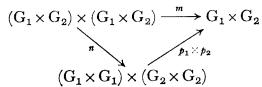
\includegraphics[keepaspectratio]{images/part002_baaabc67.jpg}}

其中 \(s(g, g') = (g', g)\)，\(m(g, g') = gg'\)，\(n(g, g') = g'g\)，这里 \(g\)、\(g'\) 取遍 \(G\)。这个图是交换的。因而 \(n_*(t \otimes t') = m_*(s_*(t \otimes t')) = m_*(t' \otimes t)\)。这个等式恰好就是 (i)。断言 (ii) 由 (i) 与命题 6 得出。

命题 8. 设 G、H 为李群，\(\phi\) 为 G 到 H 的态射。若 \(t \in \mathcal{T}^{(\infty)}(G)\)，则 \(\phi_{*}(t^{\vee}) = (\phi_{*}(t))^{\vee}\)。

设 \(\theta\)（相应地 \(\theta'\)）为 G 到 G（相应地 H 到 H）的映射 \(g \mapsto g^{-1}\)。于是 \(\phi \circ \theta = \theta' \circ \phi\)，从而 \(\phi_*(\theta_*(t)) = \theta'_*(\phi_*(t))\)。

命题 9. 设 \(\mathrm{G}_1, \cdots, \mathrm{G}_n\) 为李群，\(\mathrm{G} = \mathrm{G}_1 \times \cdots \times \mathrm{G}_n\)。若向量空间 \(\mathcal{T}^{(\infty)}(\mathrm{G})\) 与 \(\mathcal{T}^{(\infty)}(\mathrm{G}_1) \otimes \cdots \otimes \mathcal{T}^{(\infty)}(\mathrm{G}_n)\) 典范地认同，则代数 \(\mathcal{T}^{(\infty)}(\mathrm{G})\) 是诸代数 \(\mathcal{T}^{(\infty)}(\mathrm{G}_1), \ldots, \mathcal{T}^{(\infty)}(\mathrm{G}_n)\) 的张量积。若 \(t_i \in \mathcal{T}^{(\infty)}(\mathrm{G}_i)\)（\(i = 1, \ldots, n\)），则

\[
\left(t _ {1} \otimes \dots \otimes t _ {n}\right) ^ {\vee} = t _ {1} ^ {\vee} \otimes \dots \otimes t _ {n} ^ {\vee}.
\]

只需考虑 \(n = 2\) 的情形。设 \(t_1, t_1'\) 属于 \(\mathcal{T}^{(\infty)}(\mathrm{G}_1)\)，\(t_2, t_2'\) 属于 \(\mathcal{T}^{(\infty)}(\mathrm{G}_2)\)。我们需要证明 \((t_1 \otimes t_2) * (t_1' \otimes t_2') = (t_1 * t_1') \otimes (t_2 * t_2')\) 以及 \((t_1 \otimes t_2)^{\vee} = t_1^{\vee} \otimes t_2^{\vee}\)。考虑图

\pandocbounded{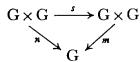
\includegraphics[keepaspectratio]{images/part002_69e6a490.jpg}}

其中 \(m((x_1, x_2), (x_1', x_2')) = (x_1x_1', x_2x_2')\)，

\[
n ((x _ {1}, x _ {2}), (x _ {1} ^ {\prime}, x _ {2} ^ {\prime})) = ((x _ {1}, x _ {1} ^ {\prime}), (x _ {2}, x _ {2} ^ {\prime})),
\]

\(p_1(x_1, x_1') = x_1x_1', p_2(x_2, x_2') = x_2x_2'\)。这个图是交换的。因而

\[
m _ {*} \left(\left(t _ {1} \otimes t _ {2}\right) \otimes \left(t _ {1} ^ {\prime} \otimes t _ {2} ^ {\prime}\right)\right) = \left(p _ {1} \otimes p _ {2}\right) _ {*} \left(n _ {*} \left(\left(t _ {1} \otimes t _ {2}\right) \otimes \left(t _ {1} ^ {\prime} \otimes t _ {2} ^ {\prime}\right)\right)\right),
\]

也就是

\[
\begin{array}{r l} (t _ {1} \otimes t _ {2}) * (t _ {1} ^ {\prime} \otimes t _ {2} ^ {\prime}) & = (p _ {1} \otimes p _ {2}) _ {*} ((t _ {1} \otimes t _ {1} ^ {\prime}) \otimes (t _ {2} \otimes t _ {2} ^ {\prime})) \\ & = p _ {1 *} (t _ {1} \otimes t _ {1} ^ {\prime}) \otimes p _ {2 *} (t _ {2} \otimes t _ {2} ^ {\prime}) \\ & = (t _ {1} * t _ {1} ^ {\prime}) \otimes (t _ {2} * t _ {2} ^ {\prime}). \end{array}
\]

同理可以看出 \((t_1\otimes t_2)^\vee = t_1^\vee \otimes t_2^\vee\)

命题 10. 设 H 为 G 的李子群，\(i: \mathrm{H} \to \mathrm{G}\) 为典范单射。于是 \(i_*\) 是代数 \(\mathcal{T}^{(\infty)}(\mathrm{H})\) 到代数 \(\mathcal{T}^{(\infty)}(\mathrm{G})\) 中的单射同态，且 \(i_*(t^\vee) = (i_*(t))^{\vee}\)（对所有 \(t \in \mathcal{T}^{(\infty)}(\mathrm{H})\)）。

这由命题 6、命题 8 以及 Differentiable and Analytic Manifolds, R, 13.2.3 得出。

\(\mathcal{T}^{(\infty)}(H)\) 借助命题 10 的同构与 \(\mathcal{T}^{(\infty)}(G)\) 的一个子代数认同。

注。若 H 是李拟子群，命题 10 仍然成立。

我们回忆 (Differentiable and Analytic Manifolds, R, 13.5.1)，若 V 是 K 上的解析流形，则 \(\mathcal{T}^{(\infty)}(\mathrm{V})\) 典范地具有一个带余单位的 K 上余代数结构；余单位是 \(\mathcal{T}^{(\infty)}(\mathrm{G})\) 到 K 中的线性映射，它把 \(\mathrm{T}_x^{(\infty)}(\mathrm{V})\) 的每个元素对应到其常数项。

命题 11. 设 G 为李群。

\begin{enumerate}
\def\labelenumi{(\roman{enumi})}
\item
  带卷积的余代数 \(\mathcal{T}^{(\infty)}(\mathbf{G})\) 是一个双代数 (Algebra, Chapter III, § 11, no. 4)。
\item
  设 \(c\) 为 \(\mathcal{T}^{(\infty)}(\mathbf{G})\) 上的余积。设 \(t \in \mathcal{T}^{(\infty)}(\mathbf{G})\)，并记
\end{enumerate}

\[
c (t) = \sum_ {i = 1} ^ {n} t _ {i} \otimes t _ {i} ^ {\prime}.
\]

于是 \(c(t^{\vee}) = \sum_{i=1}^{n} t_{i}^{\vee} \otimes t_{i}^{\prime\vee}\)。

我们证明 (i)。在所引的双代数定义中，条件 (1) 由命题 2 与命题 3 得出，条件 (2) 由 Differentiable and Analytic Manifolds, R, 13.5.1 得出。设 \(d\) 为映射 \(g \mapsto (g, g)\)（从 G 到 \(\mathrm{G} \times \mathrm{G}\)）。于是 \(c = d_{*}\)，因而 \(c\) 是代数态射（命题 6 与命题 9），这就是条件 (3)。设 \(t \in \mathrm{T}_{g}^{\infty}(\mathrm{G})\)、\(t' \in \mathrm{T}_{g'}^{\infty}(\mathrm{G})\) 都没有常数项，且 \(\lambda\)、\(\lambda'\) 是 K 的元素；于是 \(\varepsilon_{g} \otimes t'\)、\(t \otimes \varepsilon_{g'}\)、\(t \otimes t'\) 都没有常数项 (Differentiable and Analytic Manifolds, R, 13.4.1)，因而 \((\lambda\varepsilon_{g} + t) * (\lambda' \varepsilon_{g'} + t')\) 的常数项是 \(\lambda\lambda'\)；于是条件 (4) 成立。

我们证明 (ii)。由命题 8 与命题 9，

\[
c (t ^ {\vee}) = d _ {*} (t ^ {\vee}) = (d _ {*} (t)) ^ {\vee} = \left(\sum_ {i = 1} ^ {n} t _ {i} \otimes t _ {i} ^ {\prime}\right) ^ {\vee} = \sum_ {i = 1} ^ {n} t _ {i} ^ {\prime \vee} \otimes t _ {i} ^ {\vee}.
\]

命题 12. 设 G、H 为两个李群，\(\phi\) 为 G 到 H 的态射。于是 \(\phi_{*}\) 是 \(\mathcal{T}^{(\infty)}(G)\) 到 \(\mathcal{T}^{(\infty)}(H)\) 的双代数态射。

这由命题 6 与 Differentiable and Analytic Manifolds, R, 13.5.1 得出。

设 \(G\) 为李群。卷积与余积在 \(U(G)\) 上的限制在 \(U(G)\) 上定义了一个双代数结构。我们有 \(U(G)^{\vee} = U(G)\)。若 \(\phi: G \to H\) 是李群态射，我们用 \(U(\phi)\) 表示映射 \(t \mapsto \phi_{*}(t)\)（从 \(U(G)\) 到 \(U(H)\)）；它是一个双代数态射。若 \(\psi: H \to L\) 是另一个李群态射，则 \(U(\psi \circ \phi) = U(\psi) \circ U(\phi)\)。若 \(\phi\) 是浸入（相应地浸没），则由 Differentiable and Analytic Manifolds, R, 13.2.3，\(U(\phi)\) 是单射的（相应地满射的）。特别地，若 \(H\) 是 \(G\) 的李子群，则 \(U(H)\) 与 \(U(G)\) 的一个子代数认同，且 \(U(H)\) 上的余积是 \(U(G)\) 上余积的限制。若 \(H\) 在 \(G\) 中是开的，则 \(U(H) = U(G)\)。若 \(G_1, G_2\) 是李群，则 \(U(G_1 \times G_2)\) 与 \(U(G_1) \times U(G_2)\) 认同。\(U(G)\) 的本原元素就是 \(T_e(G)\) 的元素 (Differentiable and Analytic Manifolds, R, 13.5.3)。

再设 \(\phi: \mathrm{G} \to \mathrm{H}\) 为李群态射。若把 \(\operatorname{gr} \mathrm{U}(\mathrm{G})\) 与 \(\mathrm{TS}(\mathrm{T}_e(\mathrm{G}))\) 认同，把 \(\operatorname{gr} \mathrm{U}(\mathrm{H})\) 与 \(\mathrm{TS}(\mathrm{T}_e(\mathrm{H}))\) 认同，则 \(\operatorname{gr} \mathrm{U}(\phi)\) 与 \(\mathrm{TS}(\mathrm{T}_e(\phi))\) 认同 (Differentiable and Analytic Manifolds, R, 13.3.5)。我们把这一点应用于同构 \(g \mapsto g^{-1}\)（从 \(\mathrm{G}\) 到 \(\mathrm{G}^{\vee}\) 上）；这时 \(\mathrm{T}_e(\phi) = -1\)，因而

\[
t \in \mathrm{U} _ {s} (\mathrm{G}) \Rightarrow t ^ {\vee} \equiv (- 1) ^ {s} t \bmod \mathrm{U} _ {s - 1} (\mathrm{G}).\tag{3}
\]

\subsection{群在流形上作用的情形}

设 \(G\) 为李群，\(X\) 为 \(C^r\) 类流形，\(f\) 为一个 \(C^r\) 类的、\(G\) 在 \(X\) 上的左作用律。若 \(t \in T_g^{(s)}(G)\)、\(u \in T_x^{(s')}(\mathbf{X})\) 且 \(s + s' \leqslant r\)，我们用 \(t * u\) 表示 \(t \otimes u\) 在 \(f_*\) 下的像。我们把乘积 \(*\) 延拓为一个仍记作 * 的双线性映射，从 \(\mathcal{T}^{(s)}(G) \times \mathcal{T}^{(s')}(\mathbf{X})\) 到 \(\mathcal{T}^{(s+s')}(\mathbf{X})\)。第 1 节的命题 1 经过明显的修改便可推广到当前的情形。

当 G 通过左平移作用在它自身上时，我们便重新得到第 1 节的定义 1。

命题 13. 设 \(t \in \mathcal{T}^{(s)}(\mathbf{G})\)，\(t' \in \mathcal{T}^{(s')}(\mathbf{G})\)，\(u \in \mathcal{T}^{(s'')}(\mathbf{X})\)，满足

\[
s + s ^ {\prime} + s ^ {\prime \prime} \leqslant r.
\]

则 \((t*t')*u=t*(t'*u)\)。

这可以像第 1 节的命题 2 那样证明。

特别地，若 \(r \leqslant \infty\)，则向量空间 \(\mathcal{T}^{(\infty)}(\mathbf{X})\) 是代数 \(\mathcal{T}^{(\infty)}(\mathbf{G})\)（带乘积 \(*\)）上的一个左模。

命题 14. (i) 设 \(g_0 \in G\)，\(\tau(g_0)\) 为映射 \(x \mapsto f(g_0, x)\)（从 \(X\) 到 \(X\)）。若 \(u \in \mathcal{T}^{(r)}(X)\)，则 \(\tau(g_0)_*u = \varepsilon_{g_0} * u\)。

\begin{enumerate}
\def\labelenumi{(\roman{enumi})}
\setcounter{enumi}{1}
\tightlist
\item
  设 \(x_0 \in \mathbf{X}\)，\(\rho(x_0)\) 为映射 \(g \mapsto f(g, x_0)\)（从 \(G\) 到 \(X\)）。若 \(t \in T^{(r)}(G)\)，则 \(\rho(x_0)_*t = t * \varepsilon_{x_0}\)。
\end{enumerate}

这可以像第 1 节的命题 3 那样证明。

特别地，若 \(u \in \mathrm{T}(\mathrm{X})\) 且 \(t \in \mathrm{T}(\mathrm{G})\)，则 \(\varepsilon_{g_0} * u\) 与 \(t * \varepsilon_{x_0}\) 分别等于 § 2 第 2 节中定义的乘积 \(g_0u\) 与 \(tx_0\)。

命题 15. 设 G（相应地 G'）为李群，X（相应地 X'）为 \(C^{r}\) 类流形。设给定了 G（相应地 G'）在 X（相应地 X'）上的一个 \(C^{r}\) 类左作用律。设 \(\phi\) 为 G 到 G' 的态射，\(\psi\) 为 X 到 X' 的一个 \(\phi\)-态射。设 \(t \in \mathcal{T}^{(s)}(G)\)、\(u \in \mathrm{T}^{(s')}(\mathrm{X})\) 满足 \(s + s' \leqslant r\)。则

\[
\psi_ {*} (t * u) = \phi_ {*} (t) * \psi_ {*} (u).
\]

这可以像第 2 节的命题 6 那样证明。

注。设 \(f\) 为一个 \(\mathbf{C}^r\) 类的、\(\mathbf{G}\) 在 \(\mathbf{X}\) 上的右作用律。若 \(t \in \mathcal{T}^{(s)}(\mathbf{G})\)、\(u \in \mathcal{T}^{(s')}(\mathbf{X})\) 且 \(s + s' \leqslant r\)，我们用 \(u * t\) 表示 \(u \otimes t\) 在 \(f_*\) 下的像。命题 13、14、15 以明显的方式移植到这一情形。

命题 16. 设 G、G' 为李群，X 为 \(C^{r}\) 类流形，且设 G（相应地 G'）在 X 上左作用（相应地右作用），使得 \((gx)g' = g(xg')\) 对所有 \(x \in X\)、\(g \in G\)、\(g' \in G'\) 成立。设 \(t \in \mathcal{T}^{(s)}(G)\)、\(t' \in \mathcal{T}^{(s')}(\mathrm{G}')\)、\(t'' \in \mathrm{T}^{(s'')}(\mathrm{X})\) 满足 \(s + s' + s'' \leqslant r\)。则

\[
(t * t ^ {\prime \prime}) * t ^ {\prime} = t * (t ^ {\prime \prime} * t ^ {\prime}).
\]

\((t*t'')*t'\)（相应地 \(t*(t''*t')\)）是 \(t\otimes t''\otimes t'\) 在 G × X × G' 到 X 的映射 \((g,x,g')\mapsto(gx)g'\)（相应地 \(g(xg')\)）下的像。

\subsection{点分布与函数的卷积}

设 G 为李群，X 为 \(C^{r}\) 类流形，\((g, x) \mapsto gx\) 为 G 在 X 上的一个 \(C^{r}\) 类左作用律。对所有 \(x \in X\)，用 \(\rho(x)\) 表示 x 的轨道映射。

定义 3. 设 \(t \in \mathcal{T}^{(s)}(\mathrm{G})\)，\(s \leqslant r\)。设 \(f: \mathrm{X} \to \mathrm{F}\) 为取值于一个分离多范空间的 \(\mathbf{C}^r\) 类函数（例如 \(\mathrm{F} = \mathrm{K}\)）。\(t\) 与 \(f\) 的卷积，记作 \(t * f\)，是 \(\mathbf{X}\) 上以 \(\mathrm{F}\) 为值域、由

\[
(t * f) (x) = \langle t ^ {\vee} * \varepsilon_ {x}, f \rangle .
\]

于是

\[
\begin{array}{l l} (t * f) (x) = \langle \rho (x) _ {*} (t ^ {\vee}), f \rangle & (\text {no. 3, Proposition 14 (ii)}) \\ = \langle t ^ {\vee}, f \circ \rho (x) \rangle & (Diff. \& Anal. Man., R, 13.2.3) \\ = \langle t, (f \circ \rho (x)) ^ {\vee} \rangle & (Diff. \& Anal. Man., R, 13.2.3). \end{array}\tag{4}
\]

注意，定义 3 也可以写成更对称的形式

\[
\langle \varepsilon_ {x}, t * f \rangle = \langle t ^ {\vee} * \varepsilon_ {x}, f \rangle .\tag{5}
\]

函数 \((g,x)\mapsto f(gx) = (f\circ \rho (x))(g)\)（\(\mathbf{G}\times \mathbf{X}\) 上的）是 \(\mathbf{C}^r\) 类的。由 Differentiable and Analytic Manifolds, R, 13.4.4，函数 \(x\mapsto \langle t^\vee,f\circ \rho (x)\rangle\) 因而是 \(\mathbf{C}^{r - s}\) 类的（若 \(s < \infty\)）。换句话说，若 \(s < \infty\)，则 \(t*f\) 是 \(\mathbf{C}^{r - s}\) 类的。

显然，\(t * f\) 线性地依赖于 \(t\) 和 \(f\)。

特别地，公式 (4) 蕴含：对 \(g \in G\)，

\[
\left(\varepsilon_ {g} * f\right) (x) = f \left(g ^ {- 1} x\right)\tag{6}
\]

也就是

\begin{enumerate}
\def\labelenumi{(\arabic{enumi})}
\setcounter{enumi}{6}
\tightlist
\item
\end{enumerate}

\[
\varepsilon_ {g} * f = \gamma (g) f.
\]

设 \(\mathbf{K} = \mathbf{R}\) 或 \(\mathbf{C}\)，\(\mathbf{G}\) 与 \(\mathbf{X}\) 都是有限维的，且 \(\mathbf{X}\) 具有一个在 \(\mathbf{G}\) 下不变的正测度。\(\varepsilon_g * f\) 的定义与 Integration, Chapter VIII, § 4, no. 1 中的定义一致（参看~同处公式 (2)）。

命题 17. 设 \(t \in \mathcal{T}^{(s)}(\mathrm{G})\)，\(t' \in \mathcal{T}^{(s')}(\mathrm{X})\)，\(f: X \to \mathrm{F}\) 为 \(\mathbf{C}^{r}\) 类函数，满足 \(s + s' \leqslant r\)。则

\[
\langle t ^ {\prime}, t * f \rangle = \langle t ^ {\vee} * t ^ {\prime}, f \rangle .
\]

\[
\begin{array}{l l} \langle t ^ {\prime}, t * f \rangle = \langle t ^ {\prime}, x \mapsto \langle t, g \mapsto f (g ^ {- 1} x) \rangle \rangle & \text { by   (4) } \\ = \langle t \otimes t ^ {\prime}, (g, x) \mapsto f (g ^ {- 1} x) \rangle & \text {(Diff. \& Anal. Man., R, 13.4.4)} \\ = \langle t ^ {\vee} \otimes t ^ {\prime}, (g, x) \mapsto f (g x) \rangle & \text {(Diff. \& Anal. Man., R, 13.2.3)} \\ = \langle t ^ {\vee} * t ^ {\prime}, f \rangle . \end{array}
\]

命题 18. 设 \(t \in \mathcal{T}^{(s)}(\mathrm{G})\)，\(t' \in \mathcal{T}^{(s')}(\mathrm{G})\)，\(f: \mathrm{X} \to \mathrm{F}\) 为 \(\mathbf{C}^r\) 类函数，满足 \(s + s' \leqslant r\)。则

\[
(t * t ^ {\prime}) * f = t * (t ^ {\prime} * f).
\]

对所有 \(x \in X\)，

\[
\begin{array}{l l} \langle \varepsilon_ {x}, (t * t ^ {\prime}) * f \rangle = \langle (t * t ^ {\prime}) ^ {\vee} * \varepsilon_ {x}, f \rangle & \text {by (5)} \\ = \langle t ^ {\prime \vee} * (t ^ {\vee} * \varepsilon_ {x}), f \rangle & \text {(Propositions 2 and 7)} \\ = \langle t ^ {\vee} * \varepsilon_ {x}, t ^ {\prime} * f \rangle & \text {(Proposition 17)} \\ = \langle \varepsilon_ {x}, t * (t ^ {\prime} * f) \rangle & \text {(Proposition 17).} \end{array}
\]

若 \(r \geqslant \infty\)，则我们看到，\(C^\infty\) 类函数（\(X\) 上、以 \(F\) 为值域）的集合是代数 \(\mathcal{T}^{(\infty)}(G)\) 上的一个左模。

命题 19. 设 \(t \in \mathcal{T}^{(s)}(\mathrm{G})\)，\(s \leqslant r\)。设 \(f\)（相应地 \(f'\)）为 \(\mathrm{C}^r\) 类函数，定义在 \(\mathbf{X}\) 上、取值于一个分离多范空间 \(\mathrm{F}\)（相应地 \(\mathrm{F}'\)）。设 \((u, u') \mapsto uu'\) 为 \(\mathrm{F} \times \mathrm{F}'\) 到一个分离多范空间 \(\mathrm{F}''\) 中的连续双线性映射，使得 \(ff'\) 是 \(\mathrm{C}^r\) 类函数，定义在 \(\mathbf{X}\) 上、取值于 \(\mathrm{F}''\)。设 \(\sum_{i=1}^{n} t_i \otimes t_i'\) 为 \(t\) 在余积下在 \(\mathcal{T}^{(s)}(\mathrm{G}) \otimes \mathcal{T}^{(s)}(\mathrm{G})\) 中的像。则

\[
t * (f f ^ {\prime}) = \sum_ {i = 1} ^ {n} (t _ {i} * f) (t _ {i} ^ {\prime} * f ^ {\prime}).
\]

设 \(x \in X\)，并用 \(\rho(x)\) 表示 x 的轨道映射。于是

\[
\begin{array}{l l} \langle \varepsilon_ {x}, t * (f f ^ {\prime}) \rangle = \langle t ^ {\vee}, (f f ^ {\prime}) \circ \rho (x) \rangle & \text {by (4)} \\ = \langle t ^ {\vee}, (f \circ \rho (x)) (f ^ {\prime} \circ \rho (x)) \rangle \\ = \sum_ {i = 1} ^ {n} \langle t _ {i} ^ {\vee}, f \circ \rho (x) \rangle \langle t _ {i} ^ {\prime \vee}, f ^ {\prime} \circ \rho (x) \rangle \\ & (\text {Diff. \& Man. Anal., R, 13.5.2}) \\ = \sum_ {i = 1} ^ {n} \langle \varepsilon_ {x}, t _ {i} * f \rangle \langle \varepsilon_ {x}, t _ {i} ^ {\prime} * f ^ {\prime} \rangle & \text {by (4).} \end{array}
\]

注 1. 设 G 为李群，X 为 \(\mathbf{C}^r\) 类流形，\((x,g)\mapsto xg\) 为 G 在 X 上的一个 \(\mathbf{C}^r\) 类右作用律。若 \(t\in \mathcal{T}^{(s)}(\mathrm{G})\)（\(s\leqslant r\)）且 \(f\colon \mathrm{X}\to \mathrm{F}\) 是 X 上的一个 \(\mathbf{C}^r\) 类函数，我们用 \(f*t\) 表示 X 上由

\[
\begin{array}{r l} \langle \varepsilon_ {x}, f * t \rangle & = \langle \varepsilon_ {x} * t ^ {\vee}, f \rangle \\ & = \langle \rho (x) _ {*} (t ^ {\vee}), f \rangle \\ & = \langle t ^ {\vee}, f \circ \rho (x) \rangle \\ & = \langle t, (f \circ \rho (x)) ^ {\vee} \rangle . \end{array}\tag{8}
\]

特别地

\[
(f * \varepsilon_ {g}) (x) = f (x g ^ {- 1})\tag{9}
\]

也就是

\[
f * \varepsilon_ {g} = \delta (g) ^ {- 1} f.\tag{10}
\]

在明显的记号下，命题 17、18、19 成为

\begin{enumerate}
\def\labelenumi{(\arabic{enumi})}
\setcounter{enumi}{10}
\tightlist
\item
\end{enumerate}

\[
\langle t ^ {\prime}, f * t \rangle = \langle t ^ {\prime} * t ^ {\vee}, f \rangle\tag{11}
\]

\[
f * (t * t ^ {\prime}) = (f * t) * t ^ {\prime}\tag{12}
\]

\[
(f f ^ {\prime}) * t = \sum_ {i = 1} ^ {n} (f * t _ {i}) (f ^ {\prime} * t _ {i} ^ {\prime}).\tag{13}
\]

命题 20. 设 \(G\)、\(G'\) 为李群，\(X\) 为 \(C^r\) 类流形，\((g, x) \mapsto gx\)（相应地 \((x, g') \mapsto xg'\)）为 \(C^r\) 类的、\(G\)（相应地 \(G'\)）在 \(X\) 上的左（相应地右）作用律。设 \((gx)g' = g(xg')\) 对所有 \(x \in X\)、\(g \in G\)、\(g' \in G'\) 成立。设 \(t \in \mathcal{T}^{(s)}(G)\)、\(t' \in \mathcal{T}^{(s')}(\mathrm{G}')\) 且 \(f: X \to F\) 为 \(C^r\) 类函数，满足 \(s + s' \leqslant r\)。则

\[
(t * f) * t ^ {\prime} = t * (f * t ^ {\prime}).
\]

对所有 \(x \in X\)，

\[
\begin{array}{l l} \langle \varepsilon_ {x}, (t * f) * t ^ {\prime} \rangle = \langle \varepsilon_ {x} * t ^ {\prime \vee}, t * f \rangle & \text { by   (8) } \\ = \langle t ^ {\vee} * (\varepsilon_ {x} * t ^ {\prime \vee}), f \rangle & \text {(Proposition 17)} \\ = \langle t ^ {\vee} * \varepsilon_ {x}, f * t ^ {\prime} \rangle & \text {(Proposition 2 and (11))} \\ = \langle \varepsilon_ {x}, t * (f * t ^ {\prime}) \rangle & \text { by   (5). } \end{array}
\]

特别地，把 G 看作通过左平移和右平移作用在它自身上。若 \(f \colon \mathbf{G} \to \mathbf{F}\) 是 G 上的 \(\mathbf{C}^r\) 类函数且 \(t \in \mathcal{T}^{(s)}(\mathbf{G})\)（\(s \leqslant r\)），则 \(t * f\) 与 \(f * t\) 当 \(s < \infty\) 时是 G 上的 \(\mathbf{C}^{r - s}\) 类函数。进而，设 \(t' \in \mathcal{T}^{(s')}(\mathbf{G})\) 满足 \(s + s' \leqslant r\)。则

\[
(t * f) * t ^ {\prime} = t * (f * t ^ {\prime}).\tag{14}
\]

特别地，\(\mathcal{C}^{\infty}(\mathrm{G})\) 是一个 \((\mathcal{T}^{(\infty)}(\mathrm{G}),\mathcal{T}^{(\infty)}(\mathrm{G}))\)-双模。公式 (5) 与 (8) 的特殊情形是

\[
\langle t, f \rangle = \left\langle \varepsilon_ {e}, t ^ {\vee} * f \right\rangle = \left\langle \varepsilon_ {e}, f * t ^ {\vee} \right\rangle .\tag{15}
\]

注 2. 设 \((g,x)\mapsto gx\) 为一个 \(\mathbf{C}^r\) 类的、\(G\) 在 \(X\) 上的左作用律。设 \(t\in \mathbf{U}_s(\mathbf{G})\)（\(s\leqslant r\)），\(\Omega\) 为 \(X\) 的开子集，\(f\colon \Omega \to F\) 为 \(\mathbf{C}^r\) 类函数。\(t*f\) 也可以由公式 (4) 或 (5) 来定义；它是定义在 \(\Omega\) 上、取值于 \(F\) 的函数，是 \(\mathbf{C}^{r - s}\) 类的（若 \(s < \infty\)）。本节的结果以明显的方式推广到这一情形。

\subsection{由群在流形上的作用所定义的点分布场}

设 \((g,x)\mapsto\lambda(g,x)=gx\) 为 G 在 X 上的一个 \(C^{r}\) 类左作用律。设 \(s\leqslant r\) 且 \(t\in U_{s}(G)\)。对所有 \(x\in X\)，有 \(t*\varepsilon_{x}\in T_{x}^{(s)}(X)\)。映射 \(x\mapsto t*\varepsilon_{x}\) 称为由 t 及 G 在 X 上的作用所定义的点分布场，有时记作 \(D_{t}^{\lambda}\) 或简记作 \(D_{t}\)。设 \(\Omega\) 为 X 的开子集，F 为分离多范空间。若 \(f\colon\Omega\to F\) 是 \(C^{r}\) 类的且 \(s\leqslant r\)，则函数 \(t^{\vee}\ast f\)（\(\Omega\) 上的）也记作 \(D_{t}.f\)。于是

\[
(D _ {t} f) (x) = \langle t * \varepsilon_ {x}, f \rangle .\tag{16}
\]

若 \(s < \infty\)，则由第 4 节，\(D_t f \in \mathcal{C}^{r-s}(\Omega, F)\)。这样，\(f \mapsto D_t f\) 是 \(\mathcal{C}^r(\Omega, F)\) 到 \(\mathcal{C}^{r-s}(\Omega, F)\) 的映射（由于记号的滥用，常记作 \(D_t\)）。

若 \(t \in \mathrm{U}_s(\mathrm{G})\)、\(t' \in \mathrm{U}_{s'}(\mathrm{G})\) 且 \(s + s' \leqslant r\)，则由第 4 节的命题 18，

\[
\mathrm{D} _ {t * t ^ {\prime}} f = \mathrm{D} _ {t ^ {\prime}} (\mathrm{D} _ {t} f)\tag{17}
\]

因而，利用上面指出的记号滥用，有

\[
\mathrm{D} _ {t * t ^ {\prime}} = \mathrm{D} _ {t ^ {\prime}} \circ \mathrm{D} _ {t}.\tag{18}
\]

设 G 与 X 都是有限维的。映射 \((t, x) \mapsto t \otimes \varepsilon_{x}\)（从 \(\mathrm{T}^{(\mathrm{s})}(\mathrm{G}) \times \mathrm{X}\) 到向量丛 \(\mathrm{T}^{(\mathrm{s})}(\mathrm{G} \times \mathrm{X})\)，cf.~Differentiable and Analytic Manifolds, R, 13.2.5）是 \(C^{r-s}\) 类的。因而 (Differentiable and Analytic Manifolds, R, 13.2.5)，映射 \((t, x) \mapsto t * \varepsilon_{x}\)（从 \(\mathrm{T}^{(\mathrm{s})}(\mathrm{G}) \times \mathrm{X}\) 到向量丛 \(\mathrm{T}^{(\mathrm{s})}(\mathrm{X})\)）是 \(C^{r-s}\) 类的。特别地，\(D_{t}\) 是 Differentiable and Analytic Manifolds, R, 14.1.6 意义下阶数 \(\leqslant s\) 且类为 \(C^{r-s}\) 的微分算子。由公式 (16)，函数 \(D_{t}f\) 就是 f 在这个微分算子下的像 (Differentiable and Analytic Manifolds, R, 14.1.4)。

我们现在不再假设 G 与 X 都是有限维的。设 \(\psi\) 为流形 X 的自同构，\(\Delta\) 为 X 上的一个点分布场。按照一般的定义，\(\Delta\) 在 \(\psi\) 下的变换是 X 上的这样一个点分布场：它在 \(\psi(x)\) 的值是 \(\psi_{*}(\Delta(x))\)；我们把这个映射记作 \(\psi(\Delta)\)。若 \(g \in G\) 且 \(\tau(g)\) 表示 X 的自同构 \(x \mapsto gx\)，则 \(\Delta\) 在 \(\tau(g)\) 下的变换也称为 \(\Delta\) 在 g 下的变换。

命题 21. 设 \(\psi\) 为与 G 的作用交换的 X 的自同构。则 \(D_{t}\) 在 \(\psi\) 下不变。

对所有 \(x \in X\)，

\[
\begin{array}{r l} (\psi (\mathrm{D} _ {t})) (\psi (x)) & = \psi_ {*} (\mathrm{D} _ {t} (x)) = \psi_ {*} (t * \varepsilon_ {x}) \\ & = t * \psi_ {*} (\varepsilon_ {x}) \quad \text {(Proposition 15)} \\ & = t * \varepsilon_ {\psi (x)} = \mathrm{D} _ {t} (\psi (x)). \end{array}
\]

命题 22. 若 \(g \in G\)，则 \(D_t\) 在 \(g\) 下的变换是 \(D_{\varepsilon_g * t * \varepsilon_{g^{-1}}}\)。

这个变换在 gx 处的值是

\[
\begin{array}{r l r} \tau (g) _ {*} (\mathrm{D} _ {t} (x)) & = \tau (g) _ {*} (t * \varepsilon_ {x}) \\ & = \varepsilon_ {g} * (t * \varepsilon_ {x}) & \text {(Proposition 14 (i))} \\ & = (\varepsilon_ {g} * t * \varepsilon_ {g^{-1}}) * \varepsilon_ {g x} & \text {(Propositions 1 and 2)} \\ & = \mathrm{D} _ {\varepsilon_ {g} * t * \varepsilon_ {g^{-1}}} (g x). \end{array}
\]

设 \((x,g)\mapsto \mu (x,g) = xg\) 为 G 在 X 上的一个 \(\mathbf{C}^r\) 类右作用律。设 \(s\leqslant r\) 且 \(t\in \mathrm{U}_{s}(\mathrm{G})\)。对所有 \(x\in \mathbf{X}\)，有 \(\varepsilon_{x}*t\in \mathrm{T}_{x}^{(s)}(\mathbf{X})\)。映射 \(x\mapsto \varepsilon_x*t\) 称为由 \(t\) 及 G 在 X 上的作用所定义的分布场，有时记作 \(\mathrm{D}_{t}^{\mu}\) 或简记作 \(\mathrm{D}_t\)。设 \(\Omega\) 为 X 的开子集。若 \(f:\Omega \to F\) 是 \(\mathbf{C}^r\) 类的，则函数 \(f*t^{\vee}\) 记作 \(\mathrm{D}_t f\)。于是

\[
\left(\mathrm{D} _ {t} f\right) (x) = \langle \varepsilon_ {x} * t, f \rangle\tag{19}
\]

且在明显的记号下，有

\begin{enumerate}
\def\labelenumi{(\arabic{enumi})}
\setcounter{enumi}{19}
\tightlist
\item
\end{enumerate}

\[
D _ {t * t ^ {\prime}} f = \mathrm{D} _ {t} (\mathrm{D} _ {t ^ {\prime}} f)\tag{20}
\]

\[
\mathrm{D} _ {t * t ^ {\prime}} = \mathrm{D} _ {t} \circ \mathrm{D} _ {t ^ {\prime}}\tag{21}.
\]

命题 21 仍然成立。设 \(g \in G\)。\(D_t\) 在 \(g\) 下的变换（即在自同构 \(x \mapsto xg\)（\(X\) 的自同构）下的变换）是 \(D_{\varepsilon_{g^{-1}} * t * \varepsilon_g}\)。

\subsection{李群上的不变点分布场}

定义 4. 设 G 为李群。G 上的一个分布场若在 G 的左（相应地右）平移下不变，则称为左不变的（相应地右不变的）。

换句话说，分布场 \(g \mapsto \Delta_g\)（\(G\) 上的）是左不变的，如果

\[
\Delta_ {g g ^ {\prime}} = \gamma (g) _ {*} \Delta_ {g ^ {\prime}} \quad \text { for } g, g ^ {\prime} \text { in } G,
\]

或者等价地，如果

\[
\Delta_ {g g ^ {\prime}} = \varepsilon_ {g} * \Delta_ {g ^ {\prime}} \quad \text { for   } g, g ^ {\prime} \text {   in   G. }
\]

它是右不变的，如果

\[
\Delta_ {g g ^ {\prime}} = \delta (g ^ {\prime - 1}) _ {*} \Delta_ {g} \quad \text { for   } g, g ^ {\prime} \text {   in   G },
\]

或者等价地，如果.

\[
\Delta_ {g g ^ {\prime}} = \Delta_ {g} * \varepsilon_ {g ^ {\prime}}, \quad \text { for   } g, g ^ {\prime} \text {   in   G. }
\]

定义 5. 设 G 为李群，\(t \in \mathrm{U}(\mathrm{G})\)。用 \(\mathbf{L}_t\) 表示 G 上的分布场 \(g \mapsto \varepsilon_g * t\)，用 \(\mathbb{R}_t\) 表示 G 上的分布场 \(g \mapsto t * \varepsilon_g\)。

换句话说，\(L_{t}\)（相应地 \(R_{t}\)）是由 t 与借助映射 \((g, g') \mapsto gg'\) 在 G 上右（相应地左）作用的 G 所定义的分布场。设 \(\Omega\) 为 G 的开子集，F 为分离多范空间；若 \(f \in \mathcal{C}^{\omega}(\Omega, \mathrm{F})\)，则 \(\mathrm{L}_{t}f = f * t^{\vee} \in \mathcal{C}^{\omega}(\Omega, \mathrm{F})\)，且

\[
\mathrm{R} _ {t} f = t ^ {\vee} * f \in \mathcal {C} ^ {\omega} (\Omega , \mathrm{F})
\]

（第 5 节）。若 G 是有限维的，则微分算子 \(L_{t}\) 与 \(R_{t}\) 是 \(C^{\omega}\) 类的（第 5 节）。

命题 23. (i) 映射 \(t \mapsto \mathbf{L}_t\)（相应地 \(t \mapsto \mathbf{R}_t\)）是向量空间 \(\mathbf{U}(\mathbf{G})\) 到 \(\mathbf{G}\) 上左（相应地右）不变分布所成的向量空间上的同构。

\begin{enumerate}
\def\labelenumi{(\roman{enumi})}
\setcounter{enumi}{1}
\item
  对 U(G) 中的 \(t, t'\)，有 \(L_{t*t'} = L_t \circ L_{t'}\)，\(R_{t*t'} = R_{t'} \circ R_t\)，\(L_t \circ R_{t'} = R_{t'} \circ L_t\)（带有第 5 节的记号滥用）。
\item
  若 \(\theta\) 是映射 \(g \mapsto g^{-1}\)（从 \(\mathbf{G}\) 到 \(\mathbf{G}\) 上），则 \(\theta(\mathbf{L}_t) = \mathbf{R}_{t^{\vee}}\)。
\item
  若 \(t \in \mathrm{U}(\mathrm{G})\) 且 \(g \in \mathrm{G}\)，则 \((\mathrm{L}_t)_g = (\mathrm{R}_{\varepsilon_g * t * \varepsilon_{g^{-1}}})_g\)。
\end{enumerate}

在 G 中，每个右平移与每个左平移交换。于是由第 5 节的命题 21，\(L_{t}\) 是左不变的。由于 \((\mathbf{L}_{t})_{e}=t\)，映射 \(t\mapsto L_{t}\) 是单射的。设 \(\Delta\) 为 G 上的左不变分布场；设 \(t=\Delta_{e}\)；于是 \(\Delta\) 与 \(L_{t}\) 在 e 处有相同的值且都是左不变的，因而 \(\Delta=L_{t}\)。这就对 \(L_{t}\) 证明了 (i)，而对 \(R_{t}\) 的论证是类似的。公式 \(L_{t*t^{\prime}}=L_{t}\circ L_{t^{\prime}}\) 与 \(R_{t*t^{\prime}}=R_{t^{\prime}}\circ R_{t}\) 由 (21) 与 (18) 得出。设 \(t\in\mathrm{U}_{s}(\mathrm{G})\)、\(t^{\prime}\in\mathrm{U}_{s^{\prime}}(\mathrm{G}), f\in\mathcal{C}^{r}(\Omega,\mathrm{F})\)，其中 \(\Omega\) 是 G 中的开集且 \(s+s^{\prime}\leqslant r\)；于是

\[
\begin{array}{r l} \mathrm{L} _ {t} \mathrm{R} _ {t ^ {\prime}} f & = \mathrm{L} _ {t} (t ^ {\prime^ {\vee}} * f) = (t ^ {\prime^ {\vee}} * f) * t \\ & = t ^ {\prime^ {\vee}} * (f * t ^ {\vee}) \quad \text {(Proposition 20)} \\ & = \mathrm{R} _ {t ^ {\prime}} \mathrm{L} _ {t} f \end{array}
\]

因而 \(\mathbf{L}_t\circ \mathbf{R}_{t'} = \mathbf{R}_{t'}\circ \mathbf{L}_t\)。由于 \(\theta\) 是 \(\mathbf{G}\) 到 \(\mathbf{G}^{\vee}\) 的同构，\(\theta (\mathrm{L}_t)\) 是 \(\mathbf{G}\) 上的一个右不变分布场；它在 \(e\) 处的值是 \(\theta^{*}(t) = t^{\vee}\)，因而 \(\theta (\mathrm{L}_t) = \mathrm{R}_{t^{\vee}}\)。最后，

\[
\left(\mathrm{L} _ {t}\right) _ {g} = \varepsilon_ {g} * t = \left(\varepsilon_ {g} * t * \varepsilon_ {g^{-1}}\right) * \varepsilon_ {g} = \left(\mathrm{R} _ {\varepsilon_ {g} * t * \varepsilon_ {g^{-1}}}\right) _ {g}.
\]

注 1. 正是 G 通过右平移在它自身上的作用定义了左不变分布场。

注 2. 设 G 是有限维的。映射

\[
(t, g) \mapsto (\mathbf {R} _ {t}) _ {g} = t * \varepsilon_ {g}
\]

（从 \(\mathrm{U}_{s}(\mathrm{G})\times\mathrm{G}\) 到 \(\mathrm{T}^{(s)}(\mathrm{G})\)）是解析向量丛的同构；因为这个映射是双射的、在每个纤维上是线性的且是解析的（第 5 节）；另一方面，设 \(\phi:\mathrm{T}^{(s)}(\mathrm{G})\to\mathrm{U}_{s}(\mathrm{G})\times\mathrm{G}\) 为其逆双射；若 \(t\in\mathrm{T}_{g}^{(s)}(\mathrm{G})\)，则 \(\phi(t)=(t*\varepsilon_{g^{-1}},g)\)，因而 \(\phi\) 是解析的。同构 \(\phi\) 称为 \(\mathrm{T}^{(s)}(\mathrm{G})\) 的右平凡化。类似地，考虑映射 \((t,g)\mapsto(\mathrm{L}_{\mathrm{t}})_{g}=\varepsilon_{g}*t\)（从 \(\mathrm{U}_{s}(\mathrm{G})\times\mathrm{G}\) 到 \(\mathrm{T}^{(s)}(\mathrm{G})\)）；其逆同构称为 \(\mathrm{T}^{(s)}(\mathrm{G})\) 的左平凡化。通过限制，我们重新得到 \(\mathrm{T}(\mathrm{G})\) 的右平凡化和左平凡化 (§2, 第 2 节)。

\subsection{李群的李代数}

设 \(\mathbf{G}\) 为李群。在 \(\mathrm{U}(\mathbf{G})\) 中，如同在任何结合代数中一样，我们记 \([t, t'] = t * t' - t' * t\)。由于 \(\mathrm{T}_{e}(\mathbf{G})\) 是 \(\mathrm{U}(\mathbf{G})\) 的本原元素之集，有 \([\mathrm{T}_{e}(\mathbf{G}), \mathrm{T}_{e}(\mathbf{G})] \subset \mathrm{T}_{e}(\mathbf{G})\) (Chapter II, § 1, no. 2, Proposition 4)。因此，括号在 \(\mathrm{T}_{e}(\mathbf{G})\) 上的限制在 \(\mathrm{T}_{e}(\mathbf{G})\) 上定义了一个李代数结构。

引理 1. 设 \(\mathbf{X}\) 与 \(\mathbf{X}'\) 为完备可赋范空间，\(\mathbf{X}_0\) 为 \(\mathbf{X}\) 中 0 的开邻域，\(f\) 为 \(\mathbf{X}_0\) 到 \(\mathbf{X}'\) 的解析映射且满足 \(f(0) = 0\)。设 \(f = f_1 + f_2 + f_3 + \dots\) 为 \(f\) 在 0 处的幂级数展开，其中 \(f_i\) 是 \(i\) 次齐次连续多项式，定义在 \(\mathbf{X}\) 上、取值于 \(\mathbf{X}'\)。设 \(t\) 为 \(\mathrm{TS}^2 (\mathbf{X})\) 的元素，把它看作 \(\mathbf{X}\) 上支集含于 \(\{0\}\) 的点分布。设 \(t' = f_{\star}(t) \in \mathrm{TS}(\mathbf{X}')\)。\(t'\) 的 1 次齐次分量是 \(\langle f_2, t \rangle\)。

设 \(t_{1}^{\prime}\) 为这个分量。于是，对 \(X^{\prime}\) 到一个多范空间中的每个连续线性映射 u，

\[
\begin{array}{l l} u (t _ {1} ^ {\prime}) = \langle t ^ {\prime}, u \rangle & \text { because   } u \text {   is   continuous   and   linear } \\ = \langle t, u \circ f \rangle & (\text { Diff.   \&   Anal.   Man.,   R,   13.2.3 }) \\ = \langle t, u \circ f _ {2} \rangle & \text { because   } t \in \mathsf {T S} ^ {2} (\mathbf {X}) \\ = u (\langle t, f _ {2} \rangle) & (\text { Diff.   \&   Anal.   Man.,   R,   13.2.2 }), \end{array}
\]

引理由此得证。

命题 24. 设 G 为李群，(U, \(\phi\) , E) 为 G 上满足 \(\phi(e) = 0\) 的卡。设 \(e\) 的开邻域 V 满足 \(\mathrm{V}^2 \subset \mathrm{U}\)。设 \(m\) 为解析映射 \((a, b) \mapsto \phi(\phi^{-1}(a)\phi^{-1}(b))\)（从 \(\phi(V) \times \phi(V)\) 到 E 中）。设

\[
m = \sum_ {i, j \geqslant 0} m _ {i, j}
\]

为 \(m\) 在 \((0,0)\) 处的幂级数展开，其中 \(m_{i,j}\) 是双次数 \((i,j)\) 的、\(\mathbf{E} \times \mathbf{E}\) 上取值于 \(\mathbf{E}\) 的双齐次连续多项式。

\begin{enumerate}
\def\labelenumi{(\roman{enumi})}
\item
  \(m_{i,0} = m_{0,j} = 0\)（对所有 \(i \neq 1\) 与 \(j \neq 1\)）。
\item
  \(m_{1,0}(a,b)=a\) 且 \(m_{0,1}(a,b)=b\)（对所有 \(a\in E\)、\(b\in E\)）。
\item
  设 \(\psi: \mathrm{T}_e(\mathrm{G}) \to \mathrm{E}\) 为 \(\phi\) 在 \(e\) 处的微分。对所有 \(u, v\)（\(\mathrm{T}_e(\mathrm{G})\) 中的元素），
\end{enumerate}

\[
\psi ([ u, v ]) = m _ {1, 1} (\psi (u), \psi (v)) - m _ {1, 1} (\psi (v), \psi (u)).
\]

\(m(a,0) = a\)，\(m(0,b) = b\)（对所有 \(a\)、\(b\)，\(\phi (\mathrm{V})\) 中的元素），这就证明了 (i) 与 (ii)。设 \(u, v\) 属于 \(\mathrm{T_e(G)}\)。把 \(\mathrm{T_0(E)}\) 与 E 认同，从而把 \(\psi\) 与 \(\mathrm{T_e}(\phi)\) 认同。\(u\) 与 \(v\) 在 \(\mathrm{T_e}(\phi)\) 下的像分别是 \(\psi (u)\) 与 \(\psi (v)\)。这些像的张量积点分布是 \((\psi(u),0)\) 与 \((0,\psi (v))\) 在 \(\mathsf{TS(E\times E)} = \mathsf{TS(E)}\times \mathsf{TS(E)}\) 中的对称积，也就是

\[
(\psi (u), 0) \otimes (0, \psi (v)) + (0, \psi (v)) \otimes (\psi (u), 0).
\]

因而 \(\phi_{*} (u * v)\) 是上述元素在映射 \(m\)（从 \(\phi(V) \times \phi(V)\) 到 \(E\) 中）下的像。它在 TS(E) 中的 1 次分量由引理 1 是

\[
x = \langle m _ {1, 1}, (\psi (u), 0) \otimes (0, \psi (v)) + (0, \psi (v)) \otimes (\psi (u), 0) \rangle .
\]

我们用下式定义一个双线性映射 \(n\colon (\mathbf{E}\times \mathbf{E})^2\to \mathbf{E}\)

\[
n ((a, b), (a ^ {\prime}, b ^ {\prime})) = m _ {1, 1} (a, b ^ {\prime}).
\]

于是 \(n((a, b), (a, b)) = m_{1,1}(a, b)\)，因而

\[
\begin{array}{l} x = \langle n, (\psi (u), 0) \otimes (0, \psi (v)) + (0, \psi (v)) \otimes (\psi (u), 0) \rangle \\ \quad = m _ {1, 1} (\psi (u), \psi (v)) + m _ {1, 1} (0, 0) = m _ {1, 1} (\psi (u), \psi (v)). \end{array}
\]

类似地，\(\phi_{*} (v * u)\) 以 \(m_{1,1}(\phi(v), \phi(u))\) 为其在 TS(E) 中的 1 次分量。由于 \(\phi([u, v])\) 是 1 次的，这就证明了 (iii)。

推论。可赋范空间 \(\mathrm{T}_e(\mathrm{G})\) 连同括号一起是一个可赋范李代数。

定义 6. 可赋范空间 \(\mathrm{T_e(G)}\) 连同括号一起称为 \(\mathbf{G}\) 的可赋范李代数，或简称为 \(\mathbf{G}\) 的李代数，记作 \(\mathbf{L(G)}\)。

命题 25. 设 \(\mathbf{G}\) 为李群，\(\operatorname{E}(\mathbf{G})\) 为 \(\mathbf{L}(\mathbf{G})\) 的包络代数。\(\mathbf{L}(\mathbf{G})\) 到 \(\operatorname{E}(\mathbf{G})\) 的典范单射定义了一个同态 \(\theta\)（从代数 \(\operatorname{E}(\mathbf{G})\) 到代数 \(\operatorname{U}(\mathbf{G})\) 中）。若 \(\mathbf{K}\) 的特征为 \(0\)，则 \(\eta\) 是双代数同构。

双代数 U(G) 是余交换的 (Differentiable and Analytic Manifolds, R, 13.5.1)，且滤过 (U \(_{s}\) (G)) 与双代数结构相容。U(G) 的本原元素之集是 L(G)。于是只需引用 Chapter II, § 1, no. 6, Theorem 1。

当 \(\mathbf{K}\) 的特征为 0 时，我们今后将把 \(\mathrm{U}(\mathrm{G})\) 与 L(G) 的包络代数认同。由 (2) 与命题 7 (ii)，U(G) 到 U(G) 的映射 \(t \mapsto t^{\vee}\) 这时与 U(G) 的主反自同构认同 (Chapter I, § 2, no. 4)。

命题 26. 设 K 的特征为 \(p > 0\)。对所有 \(a \in \mathrm{L}(\mathrm{G})\)，有 \(a^p \in \mathrm{L}(\mathrm{G})\) 且 \(\operatorname{ad}(a^p) = (\operatorname{ad} a)^p\)（幂 \(a^p\) 是在 \(\mathrm{U}(\mathrm{G})\) 中计算的）。

若 \(a \in \mathrm{L}(\mathrm{G})\)，则 \(a\) 在 \(\mathrm{U}(\mathrm{G})\) 中是本原的，因而 \(a^p\) 在 \(\mathrm{U}(\mathrm{G})\) 中是本原的 (Chapter II, § 1, no. 2, Remark 1)，于是 \(a^p \in \mathrm{L}(\mathrm{G})\)。设 \(\sigma_a\)（相应地 \(\tau_a\)）为线性映射 \(x \mapsto a * x\)（相应地 \(x \mapsto x * a\)），它从 \(\mathrm{U}(\mathrm{G})\) 到 \(\mathrm{U}(\mathrm{G})\) 中。对所有 \(x \in \mathrm{U}(\mathrm{G})\)，(ad \(a\) ) \((x) = (\sigma_a - \tau_a)(x)\)，因而 (ad \(a\) ) \(^p = (\sigma_a - \tau_a)^p\)。但 \(\sigma_a\) 与 \(\tau_a\) 交换，故 \((\sigma_a - \tau_a)^p = (\sigma_a)^p - (\tau_a)^p = \tau_a^p - \sigma_a^p\)，由此得第二个断言。

定义 7. 设 X 为 \(\mathbf{C}^r\) 类流形（\(r \geqslant 2\)），\(\mathfrak{g}\) 为完备可赋范李代数。一个 \(\mathbf{C}^{r-1}\) 类的、\(\mathfrak{g}\) 在 X 上的无穷小左（相应地右）作用律是指映射 \(a \mapsto \mathbf{D}_a\)（从 \(\mathfrak{g}\) 到 X 上向量场的集合），它满足下列性质：

\begin{enumerate}
\def\labelenumi{(\alph{enumi})}
\item
  映射 \((a, x) \mapsto \mathrm{D}_a(x)\) 是一个 \(\mathbf{C}^{r-1}\) 类态射（从平凡向量丛 \(g \times X\) 到向量丛 \(\mathrm{T}(X)\)）；
\item
  \([\mathrm{D}_a,\mathrm{D}_b] = -\mathrm{D}_{[a,b]}\)（相应地 \([\mathrm{D}_a,\mathrm{D}_b] = \mathrm{D}_{[a,b]})\)）（对所有 \(a,b\)，\(\mathfrak{g}\) 中的元素）。
\end{enumerate}

特别地，每个向量场 \(\mathbf{D}_a\) 都是 \(\mathbf{C}^{r - 1}\) 类的。

注。设 X 为 \(C^{r}\) 类流形，g 为有限维李代数，\(a \mapsto D_{a}\) 为 g 到 X 上 \(C^{r-1}\) 类向量场的向量空间中的一个线性映射。于是定义 7 的条件 (a) 成立。因为，通过取 g 的一个基并引用 Differentiable and Analytic Manifolds, R, 7.7.1，问题就化为 dim g = 1 的情形，而这时我们的断言是明显的。

命题 27. 设 G 为李群，X 为 \(\mathbf{C}^r\) 类流形。设给定了 G 在 X 上的一个 \(\mathbf{C}^r\) 类左（相应地右）作用律。对所有 \(a \in \mathrm{L}(\mathrm{G})\)，用 \(\mathrm{D}_a\) 表示由 \(a\) 在 X 上定义的点分布场。

\begin{enumerate}
\def\labelenumi{(\roman{enumi})}
\item
  映射 \((a, x) \mapsto \mathrm{D}_a(x)\) 是一个 \(\mathbf{C}^{r-1}\) 类态射（从平凡向量丛 \(\mathbf{L}(\mathbf{G}) \times \mathbf{X}\) 到向量丛 \(\mathrm{T}(\mathbf{X})\)）。
\item
  设 \(\mathbf{I}\) 为 \(\mathbf{K}\) 中包含 0 的开子集，\(\gamma: \mathbf{I} \to \mathbf{G}\) 为 \(\mathbf{C}^r\) 类映射且满足 \(\gamma(0) = e\)。设 \(a = \mathrm{T}_0(\gamma) 1 \in \mathbf{L}(\mathbf{G})\)。若 \(f\) 是 \(\mathbf{C}^r\) 类函数，定义在 \(\mathbf{X}\) 的某个开子集上，则
\end{enumerate}

\((D_{a}f)(x) = \lim_{k\in \mathbb{K}^{*},k\to 0}k^{-1}(f(\gamma (k)x) - f(x))\)（若 G 左作用），

\[
(D _ {a} f) (x) = \lim _ {k \in K ^ {*}, k \rightarrow 0} k ^ {- 1} (f (x \gamma (k)) - f (x)) \quad \text {if } G \text { operates on the right}.
\]

\begin{enumerate}
\def\labelenumi{(\roman{enumi})}
\setcounter{enumi}{2}
\tightlist
\item
  若 \(r \geqslant 2\)，则映射 \(a \mapsto \mathbf{D}_a\) 是一个 \(\mathbf{C}^{r-1}\) 类的、\(\mathbf{L}(\mathbf{G})\) 在 \(\mathbf{X}\) 上的无穷小左（相应地右）作用律。
\end{enumerate}

设 G 左作用在 X 上。设 \(\phi: G \times X \to X\) 为该作用律。于是 \(T(\phi)\) 是一个 \(\phi\)-态射，为 \(C^{r-1}\) 类，从向量丛 \(T(G) \times T(X)\) 到向量丛 \(T(X)\) 中 (Differentiable and Analytic

Manifolds, R, 8.1.2)。诱导向量丛 \((\mathrm{T}(\mathrm{G}) \times \mathrm{T}(\mathrm{X}))|(\{e\} \times \mathrm{X})\) 与 \(\mathrm{E} = \mathrm{L}(\mathrm{G}) \times \mathrm{T}(\mathrm{X})\) 认同。因而 \(\mathrm{T}(\phi)|\mathrm{E}\) 是 \(\mathbf{C}^{r-1}\) 类向量丛态射。对 \((a, x) \in \mathrm{L}(\mathrm{G}) \times \mathrm{X}\)，有 \(\mathrm{T}(\phi)(a, x) = \mathbf{D}_{a}(x)\)，由此得 (i)。

给出 \((\mathrm{D}_a f)(x)\) 的公式由 §2 第 2 节末尾以及 Differentiable and Analytic Manifolds, R, 8.4.5 得出。

设 \(r \geqslant 2\)。设 \(a, b\) 属于 \(\mathbf{L}(\mathbf{G})\)，\(f\) 为 \(\mathbf{C}^r\) 类函数，定义在 \(\mathbf{X}\) 的某个开子集上。于是

\[
\begin{array}{l l} \mathrm{D} _ {[ a, b ]} f = \mathrm{D} _ {b} (\mathrm{D} _ {a} f) - \mathrm{D} _ {a} (\mathrm{D} _ {b} f) & \text { by   (17) } \\ = [ \mathrm{D} _ {b}, \mathrm{D} _ {a} ] f & (\text { Diff.   \&   Anal.   Man.,   R,   8.5.3 }). \end{array}
\]

设 \(x \in X\)。取 \(f\) 为 \(x\) 的某开邻域上的一个卡，便得 \(D_{[a,b]}(x) = [D_b, D_a](x)\)，由此得 (iii)。若 \(G\) 右作用在 \(X\) 上，论证是类似的。

当 \(r \geqslant 2\) 时，映射 \(a \mapsto D_{a}\) 称为与所给作用律相伴的无穷小作用律。

\subsection{李代数的函子性质}

设 \(G\) 与 \(H\) 为李群，\(\phi\) 为 \(G\) 到 \(H\) 的态射。\(U(\phi)\) 在 \(L(G)\) 上的限制（它正是 \(T_e(\phi)\)）是 \(L(G)\) 到 \(L(H)\) 的连续态射，我们把它记作 \(L(\phi)\)。若 \(\psi\) 是 \(H\) 到某个李群的态射，则 \(L(\psi \circ \phi) = L(\psi) \circ L(\phi)\)。

为使 \(\phi\) 是浸入，充要条件是 \(\mathrm{L}(\phi)\) 是 \(\mathrm{L}(\mathrm{G})\) 到 \(\mathrm{L}(\mathrm{H})\) 的某个具有拓扑余的子代数上的同构。特别地，若 \(\mathrm{G}\) 是 \(\mathrm{H}\) 的李子群且 \(\phi\) 是典范单射，则 \(\mathrm{L}(\mathrm{G})\) 与 \(\mathrm{L}(\mathrm{H})\) 的一个李子代数借助 \(\mathrm{L}(\phi)\) 认同。更特殊地，若 \(\mathrm{G}\) 是 \(\mathrm{H}\) 的开子群，则 \(\mathrm{L}(\mathrm{G}) = \mathrm{L}(\mathrm{H})\)。

若 G 是 H 的李拟子群，则 L(G) 也与 L(H) 的一个闭李子群认同。

为使 \(\phi\) 是浸没，充要条件是 \(\mathrm{L}(\phi)\) 是满射的且其核具有拓扑余。这时，\(N\)（\(\phi\) 的核）是 \(G\) 的李子群且 \(\mathrm{L}(N) = \mathrm{Ker} \, L(\phi)\)。特别地，若 \(H\) 是 \(G\) 关于一个正规李子群 \(P\) 的商李群，则 \(L(P)\) 是 \(\mathrm{L}(G)\) 的理想，且若 \(\phi\) 是 \(G\) 到 \(H\) 上的典范满射，则 \(\mathrm{L}(G/P)\) 与 \(\mathrm{L}(G)/\mathrm{L}(P)\) 借助由 \(\mathrm{L}(\phi)\) 过渡到商而导出的态射认同。

设 \(I\) 为有限集，\((\mathbf{G}_{i})_{i\in I}\) 为李群族，\(G\) 为它们的积，\(p_i\) 为 \(G\) 到 \(G_i\) 上的典范态射。于是 \((\mathrm{L}(p_i))_{i\in I}\) 是李代数 \(L(G)\) 到李代数 \(\prod_{i\in I} L(G_i)\) 中的态射，且是可赋范空间之间的同构。因而 \(L(G)\) 与 \(\prod_{i\in I} L(G_i)\) 借助 \((L(p_i))_{i\in I}\) 认同。

命题 28. 设 G 与 H 为李群，\(\phi\) 为 G 到 H 的态射。设 K 的特征为 0 且 H 是有限维的。

\begin{enumerate}
\def\labelenumi{(\roman{enumi})}
\item
  \(\phi\) 的核 N 是 \(\mathbf{G}\) 的李子群，且 \(\mathrm{L}(\mathbf{N}) = \mathrm{Ker} \, \mathrm{L}(\phi)\)。
\item
  态射 \(\psi\)（由 \(\phi\) 过渡到商而导出的、G/N 到 H 中的）是浸入。
\item
  若 \(\phi(\mathbf{G})\) 在 \(\mathbf{H}\) 中是闭的且 \(\mathbf{G}\) 的拓扑具有可数基，则 \(\phi(\mathbf{G})\) 是 \(\mathbf{H}\) 的李子群，\(\psi\) 是李群 \(\mathbf{G}/\mathbf{N}\) 到李群 \(\phi(\mathbf{G})\) 上的同构，且 \(\mathbf{L}(\phi(\mathbf{G})) = \mathbf{Im} \mathbf{L}(\phi)\)。
\end{enumerate}

设 G 通过映射 \((g, h) \mapsto \phi(g)h\) 左作用在 H 上。只需对 e 的轨道引用 §1 第 7 节的命题 14。

命题 29. 设 G 与 H 为李群，\(\phi\) 为 G 到 H 的态射。设 K 的特征为 0 且 H 是有限维的。若 H' 是 H 的李子群，则 G' = \(\phi^{-1}(\mathrm{H}')\) 是 G 的李子群且 L(G') = L(φ)\(^{-1}\)(L(H'))。

设 \(\pi\) 为 H 到齐性空间 \(\mathbf{X} = \mathbf{H} / \mathbf{H}'\) 的典范映射。设 G 左作用在 \(\mathbf{X}\) 上，作用映射为 \((g, x) \mapsto \phi(g)x\)。\(\pi(e)\) 的稳定子群是 \(G'\)，因而它是 G 的李子群 (§ 1, 第 7 节, 命题 14)。\(\pi(e)\) 的轨道映射是 \(\pi \circ \phi\)。由 § 1 的命题 14，L(G') 是 L(\(\pi \circ \phi\)) = \(T_e(\pi)\) \(\circ\) L(\(\phi\)) 的核。\(T_e(\pi)\) 的核是 L(H') (§ 1, 第 6 节, 命题 11 (i))，因而 Ker L(\(\pi \circ \phi\)) = L(\(\phi\)) \(^{-1}\)(L(H'))。

推论 1. 设 \(\mathbf{G}\)、\(\mathbf{H}\) 为李群，\(\phi_1\) 与 \(\phi_2\) 为 \(\mathbf{G}\) 到 \(\mathbf{H}\) 的态射。设 \(\mathbf{K}\) 的特征为 0 且 \(\mathbf{H}\) 是有限维的。由 \(g \in \mathbf{G}\)（满足 \(\phi_1(g) = \phi_2(g)\)）组成的集合是李子群 \(\mathbf{G}'\)（\(\mathbf{G}\) 的李子群），且 \(\mathbf{L}(\mathbf{G}')\) 是由 \(x \in \mathbf{L}(\mathbf{G})\)（满足 \(\mathrm{L}(\phi_1)x = \mathrm{L}(\phi_2)x\)）组成的集合。

我们记 \(\phi(g) = (\phi_1(g), \phi_2(g))\)（对所有 \(g \in G\)），于是 \(\phi\) 是 \(G\) 到 \(H \times H\) 的态射。设 \(\Delta\) 为 \(H \times H\) 的对角子群。于是 \(G' = \phi^{-1}(\Delta)\)，且 \(L(\phi)x = (L(\phi_1)x, L(\phi_2)x)\)（对所有 \(x \in L(G)\)）。现在只需引用命题 29。

推论 2. 设 \(\mathbf{G}\) 为有限维李群，\(\mathbf{G}_1\) 与 \(\mathbf{G}_2\) 为 \(\mathbf{G}\) 的两个李子群。设 \(\mathbf{K}\) 的特征为 0。则 \(G_1 \cap G_2\) 是 \(\mathbf{G}\) 的李子群，其李代数为 \(\mathbf{L}(\mathbf{G}_1) \cap \mathbf{L}(\mathbf{G}_2)\)。

我们对 \(\mathbf{G}_1\) 到 \(\mathbf{G}\) 的典范单射与子群 \(\mathbf{G}_2\) 应用命题 29。

推论 3. 设 G、G'、H 为李群，\(\phi: G \to H\) 与 \(\phi': G' \to H\) 为李群态射。设 K 的特征为 0 且 H 是有限维的。设 F 为由 \((g, g') \in G \times G'\)（满足 \(\phi(g) = \phi'(g')\)）组成的集合。则 F 是 \(G \times G'\) 的李子群，且 L(F) 是由 \((x, x') \in L(G) \times L(G')\)（满足 L( \(\phi\) ) \(x = L(\phi')x'\)）组成的集合。

我们对态射 \((g, g') \mapsto \phi(g)\) 与 \((g, g') \mapsto \phi'(g')\)（从 \(G \times G'\) 到 \(H\) 中）应用推论 1。

命题 30. 设 G 为具有可数基的有限维李群，且

H 与 H' 为 G 的李子群。设 K 的特征为 0 且 HH' 在 G 中是局部闭的。

\begin{enumerate}
\def\labelenumi{(\roman{enumi})}
\item
  HH' 是 G 的子流形，且 \(\mathrm{T}_{e}(\mathrm{HH}') = \mathrm{L}(\mathrm{H}) + \mathrm{L}(\mathrm{H}')\)。
\item
  设 H 的每个元素与 H' 的每个元素交换。则 HH' 是 G 的李子群。设 \(\phi\) 为映射 \((h, h') \mapsto hh'\)（从 H \(\times\) H' 到 HH' 上）。\(\phi\) 的核是对 \((m, m^{-1})\)（其中 \(m \in \mathrm{H} \cap \mathrm{H}'\)）组成的集合，且 \((\mathrm{H} \times \mathrm{H}') / \mathrm{Ker} \phi\) 到 HH' 上的、由 \(\phi\) 过渡到商而导出的态射是李群同构。
\end{enumerate}

设 \(\mathbf{H} \times \mathbf{H}'\) 右作用在 \(\mathbf{G}\) 上，作用映射为 \(((h, h'), g) \mapsto hgh'^{-1}\)。设 \(\rho\) 为 \(e\) 的轨道映射：\((h, h') \mapsto hh'^{-1}\)。由 § 1 第 7 节的命题 14 (iii)，HH' 是 \(\mathbf{G}\) 的子流形且 \(\mathrm{T}_e(\mathrm{HH}') = \mathrm{Im} \mathrm{T}_e(\rho)\)。现在

\[
\mathrm{T} _ {e} (\rho) (\mathrm{L} (\mathrm{H}) \times \{0 \}) = \mathrm{L} (\mathrm{H}) \quad \text { and } \quad \mathrm{T} _ {e} (\rho) (\{0 \} \times \mathrm{L} (\mathrm{H} ^ {\prime})) = \mathrm{L} (\mathrm{H} ^ {\prime})
\]

因而 \(\mathrm{T}_{e}(\mathrm{HH}^{\prime})=\mathrm{L}(\mathrm{H})+\mathrm{L}(\mathrm{H}^{\prime})\)。设 H 的每个元素与 \(H^{\prime}\) 的每个元素交换。则 \(HH^{\prime}\) 是 G 的子群。由 (i)，它是 G 的李子群。断言的其余部分由命题 28 得出。

命题 31. 设 G 为具有可数基的有限维李群，H 为 G 的正规李子群，A 为 G 的李子群。设 K 的特征为 0 且 AH 是闭的。设 \(\phi\) 为 G 到 G/H 上的典范态射。则典范映射

\[
\mathrm{A} / (\mathrm{H} \cap \mathrm{A}) \rightarrow \phi (\mathrm{A}), \quad \mathrm{AH} / \mathrm{H} \rightarrow \phi (\mathrm{A})
\]

都是李群同构。

由命题 30，AH 是 G 的李子群。由命题 29 的推论 2，H ∩ A 是 G 的李子群。因此谈论群 AH/H 与 A/(H ∩ A) 是有意义的。另一方面，φ(A) 是 AH 在 G/H 中的典范像，它是闭的，因而是 G/H 的李子群（命题 28 (iii)）。把命题 28 应用于复合态射 A → G → G/H 与 AH → G → G/H，便证明了命题中的典范映射是李群同构。

命题 32. 设 G 与 H 为李群，k 为 K 的非离散闭子域，\(\phi\) 为 \(k\) 上的李群结构之间 G 到 H 的态射。设 K 的特征为 0。若 \(L(\phi)\) 是 K-线性的，则 \(\phi\) 是 K 上的李群结构之间的态射。

对所有 \(g \in G\)，

\[
\mathrm{T} _ {g} (\phi) = \mathrm{T} _ {e} (\gamma (\phi (g))) \circ \mathrm{L} (\phi) \circ \mathrm{T} _ {g} (\gamma (g) ^ {- 1})
\]

因而 \(\mathrm{T}_g(\phi)\) 是 K-线性的。命题于是由 Differentiable and Analytic Manifolds, R, 5.14.6 得出。

\subsection{代数可逆元群的李代数}

设 A 为带单位元 \(e\) 的完备可赋范结合代数。设 \(\mathbf{A}^*\) 为 A 的可逆元群。我们已看到 (§ 1, no. 1)，\(\mathbf{A}^*\) 是 A 的开子流形且是一个李群。设 \(\mathbf{G}\) 为李群，\(f\) 为李群 \(\mathbf{G}\) 到李群 \(\mathbf{A}^*\) 的态射，\(f\) 可以看作 \(\mathbf{G}\) 到完备可赋范空间 A 的解析映射。因而，若 \(t \in \mathcal{T}^{(\infty)}(\mathbf{G})\)，我们可以构造 \(\langle t, f \rangle\)，它是 A 的一个元素。

命题 33. 映射 \(t \mapsto \langle t, f \rangle\) 是代数 \(\mathcal{T}^{(\infty)}(G)\) 到代数 A 中的态射。

只需验证：若 \(t\) 与 \(t'\) 是 \(G\) 上的点分布，则 \(\langle t * t', f \rangle = \langle t, f \rangle \langle t', f \rangle\)。但

\[
\begin{array}{r l} \langle t * t ^ {\prime}, f \rangle & = \langle t \otimes t ^ {\prime}, (g, g ^ {\prime}) \mapsto f (g g ^ {\prime}) \rangle \\ & = \langle t \otimes t ^ {\prime}, (g, g ^ {\prime}) \mapsto f (g) f (g ^ {\prime}) \rangle \\ & = \langle t, f \rangle \langle t ^ {\prime}, f \rangle \\ & \quad (Diff. \& Anal. Man., R, 13.4.3). \end{array}
\]

命题 33 的态射称为与 f 相伴的态射。

取 G 为群 A* 自身，取 f 为 A* 的恒等映射 \(\iota\)。我们得到代数 \(\mathcal{T}^{(\infty)}(\mathbf{A}^*)\) 到代数 A 中的一个称为典范的态射。切空间 \(\mathrm{T}_{e}(\mathbf{A}^*)\) 典范地与 A 认同；且若 \(t \in \mathrm{T}_{e}(\mathbf{A}^*)\)，则这个认同的定义使得 \(\langle t, \iota \rangle = t\)。于是命题 33 蕴含下述推论：

推论。典范映射 \(\zeta\)（从 \(\mathbf{L}(\mathbf{A}^{*})\) 到 \(\mathbf{A}\)）是李代数 \(\mathbf{L}(\mathbf{A}^{*})\) 到李代数 \(\mathbf{A}\) 上的同构。换句话说，

\[
\zeta ([ a, b ]) = \zeta (a) \zeta (b) - \zeta (b) \zeta (a)
\]

对所有 \(a, b\)（\(\mathrm{L}(\mathbf{A}^*)\) 中的元素）成立。若 \(\mathbf{K}\) 的特征为 \(p > 0\)，则 \(\zeta(a^p) = \zeta(a)^p\)（对所有 \(a \in \mathrm{L}(\mathbf{A}^*)\)）。

今后我们借助同构 ζ 把 L(A*) 与 A 认同。

\(\mathcal{T}^{(\infty)}(\mathbf{A}^*)\) 到 \(\mathbf{A}\) 的典范态射是作为命题 33 的态射的特殊情形而得到的。但也可以沿相反的方向论证：

命题 34. 设 H 为李群，A 为含单位元的完备可赋范结合代数，\(\phi: \mathrm{H} \to \mathrm{A}^*\) 为李群态射。相伴态射 \(\phi'\)（\(\mathcal{T}^{(\infty)}(\mathrm{H})\) 到 A 中的）是由 \(\phi_*\) 与 \(\mathcal{T}^{(\infty)}(\mathrm{A}^*)\) 到 A 的典范态射复合而得。特别地，\(\phi'(x) = \mathrm{L}(\phi)(x)\)（对所有 \(x \in \mathrm{L}(\mathrm{H})\)）。

设 \(i\) 为 \(\mathbf{A}^*\) 到 A 的恒等映射。于是，对所有 \(t\in \mathcal{T}^{(\infty)}(\mathrm{H})\)，

\[
\begin{array}{r l} \phi^ {\prime} (t) = \langle t, \phi \rangle & = \langle t, i \circ \phi \rangle \\ & = \langle \phi_ {*} (t), i \rangle \quad (Diff. \& Anal. Man., R, 13.2.3). \end{array}
\]

\subsection{某些线性群的李代数}

设 \(\mathbf{E}\) 为完备可赋范空间。于是 \(\mathcal{L}(\mathbf{E})\) 是含单位的完备可赋范代数，而 \(\mathbf{GL}(\mathbf{E})\) 是李群。由第 9 节命题 33 的推论，若把 \(\mathrm{T}_{1}(\mathbf{GL}(\mathbf{E}))\) 典范地与 \(\mathcal{L}(\mathbf{E})\) 认同，则 \(\mathrm{L}(\mathbf{GL}(\mathbf{E}))\) 上的李代数结构由括号 \((x,y)\mapsto xy - yx\)（\(\mathcal{L}(\mathbf{E})\) 的两个元素的括号）给出。特别地，\(\mathrm{L}(\mathbf{GL}(n,\mathbf{K}))\) 典范地与 \(\mathrm{gl}(n,\mathbf{K})\) 认同 (Chapter I, §1, no. 2)。

命题 35. 设 E 为有限维向量空间。设 \(\phi\) 为态射 \(g \mapsto \det g\)（从李群 \(\mathbf{GL}(E)\) 到李群 \(\mathbf{K}^*\) 中）。\(\mathrm{L}(\phi)\)（从 \(\mathcal{L}(E)\) 到 \(\mathbf{K}\)）是映射 \(x \mapsto \mathrm{Tr}x\)。\(\mathbf{SL}(E)\)（\(\phi\) 的核）是 \(\mathbf{GL}(E)\) 的李子群，其李代数为 \(\mathfrak{sl}(E)\)。

我们选取 E 的一个范数和一个基。行列式的展开式证明：

\[
\det (1 + u) \in 1 + \operatorname{Tr} u + o (\| u \|)
\]

当 \(u\) 在 \(\mathcal{L}(\mathrm{E})\) 中趋于 0 时成立。因而，对 \(x \in \mathcal{L}(\mathrm{E}) = \mathrm{L}(\mathbf{GL}(\mathrm{E}))\)，利用第 9 节的命题 34，得

\[
\mathrm{L} (\phi) (x) = \langle x, \phi \rangle = \operatorname{Tr} x.
\]

由此可得 \(\phi\) 是浸没。因此，\(\operatorname{Ker} \phi = \mathbf{SL}(E)\) 是 \(\mathbf{GL}(E)\) 的李子群，其李代数为 \(\operatorname{Ker} L(\phi) = \mathfrak{sl}(E)\)。

设 \(\mathbf{E}_1, \ldots, \mathbf{E}_n\) 为完备可赋范空间，\(\mathbf{E}\) 为它们的直和。每个 \(x \in \mathcal{L}(\mathbf{E})\) 都可以表示为一个矩阵 \((x_{ij})_{1 \leqslant i, j \leqslant n}\)，其中 \(x_{ij} \in \mathcal{L}(\mathbf{E}_i, \mathbf{E}_j)\)。

命题 36. 设 \(\mathbf{I}\) 为 \(\{1,2,\ldots,n\}\) 的子集，\(\mathbf{G}\) 为 \(\mathbf{GL}(\mathbf{E})\) 中由 \(g = (g_{ij})_{1\leqslant i,j\leqslant n}\in \mathbf{GL}(\mathbf{E})\)（满足 \(g_{ij} = 0\)（当 \(i < j\)）且 \(g_{ii} = 1\)（当 \(i\in \mathbf{I}\)））组成的子群。则 \(\mathbf{G}\) 是 \(\mathbf{GL}(\mathbf{E})\) 的李子群，且 \(\mathbf{L}(\mathbf{G})\) 是由 \(x = (x_{ij})_{1\leqslant i,j\leqslant n}\in \mathcal{L}(\mathbf{E})\)（满足 \(x_{ij} = 0\)（当 \(i < j\)）且 \(x_{ii} = 0\)（当 \(i\in \mathbf{I}\)））组成的集合。设 \(\mathbf{S}\) 为由 \((x_{ij})\in \mathcal{L}(\mathbf{E})\)（满足 \(x_{ij} = 0\)（当 \(i < j\)）且 \(x_{ii} = 0\)（当 \(i\in \mathbf{I}\)））组成的集合。则 \(\mathbf{G}\) 是 \(\mathbf{GL}(\mathbf{E})\) 与仿射子空间 \(1 + \mathbf{S}\)（\(\mathcal{L}(\mathbf{E})\) 的）的交。因而 \(\mathbf{G}\) 是 \(\mathbf{GL}(\mathbf{E})\) 的子流形，且 \(\mathbf{G}\) 在 1 处的切空间与 \(\mathbf{S}\) 认同。

特别地，在 \(\mathbf{GL}(n,\mathbf{K})\) 中，按 Integration, Chapter VII, § 3, no. 3 定义的 全下三角形子群与严格下三角形子群是分别以 \(t(n,\mathbf{K})\) 与 \(n(n,\mathbf{K})\) 为李代数的李子群 (Chapter I, § 1, no. 2)。

命题 37. 设 A 为完备可赋范含单位结合代数，\(x \mapsto x^t\) 为 A 到 A 中的连续线性映射，满足 \((x^t)^t = x\) 且 \((xy)^t = y^t x^t\)（对所有 \(x, y\)，A 中的元素）。设 K 的特征 \(\neq 2\)。设 G 为 A* 中由 \(x \in A\)（满足 \(xx^t = x^t x = 1\)）组成的子群。则 G 是 A* 的李子群，且 L(G) 是由 \(y \in A\)（满足 \(y^t = -y\)）组成的集合。

设 \(S\)（相应地 \(S'\)）为 \(y \in A\) 中满足 \(y = y^t\)（相应地 \(y = -y^t\)）者组成的集合。则 \(S, S'\) 是 \(A\) 的闭向量子空间。公式

\[
y = \frac {1}{2} (y + y ^ {t}) + \frac {1}{2} (y - y ^ {t})
\]

证明 A 是 S 与 \(S'\) 的拓扑直和。设 f 为 A 到 S 中由 \(f(x) = xx^{t}\) 定义的映射。这个映射是解析的。对所有 \(y \in A\)，\(f(1 + y) = 1 + y + y^{t} + yy^{t}\)；在 A 上选取一个与其代数结构相容的范数；则

\[
f (1 + y) \in 1 + y + y ^ {t} + o (\| y \|) \quad \text { for   } y \text {   tending   to   } 0.
\]

于是，\(\mathrm{T}_{1}(f)(y)=y+y^{t}\)，从而 f 在 1 处是浸没。因此，存在 A 中 1 的开邻域 U，使得 \(U\cap G\) 是 U 的子流形。因而 (§ 1, no. 3, Proposition 6) G 是 \(A^{*}\) 的李子群。此外，\(\mathrm{L}(G)=\mathrm{T}_{e}(G)=\mathrm{Ker}\;\mathrm{T}_{1}(f)\)。

推论 1. 设 K 的特征 \(\neq 2\)。设 E 为 K 上的有限维向量空间，\(\phi\) 为 E 上的非退化对称（相应地交错）双线性型。对所有 \(u \in \mathcal{L}(\mathrm{E})\)，用 \(u^*\) 表示 \(u\) 关于 \(\phi\) 的伴随。设 G 为 \(\phi\) 的正交群（相应地辛群）。则 G 是 \(\mathbf{GL}(\mathrm{E})\) 的李子群，且 \(\mathrm{L}(\mathrm{G})\) 是由 \(x \in \mathcal{L}(\mathrm{E})\)（满足 \(x^* = -x\)）组成的集合。

我们对 A = L(E) 且 \(x^{t} = x^{*}\) 的情形应用命题 37。

注。设 B 为 E 的一个基，J 为 \(\phi\) 关于 B 的矩阵。则 \(\mathrm{L}(G)\) 是 \(\mathcal{L}(\mathrm{E})\) 中其关于 B 的矩阵 X 满足方程

\[
{ } ^ { t } X = - J X J ^ { - 1 } .
\]

这由 Algebra, Chapter IX, § 1, formula (50) 得出。

推论 2. 设 E 为复（相应地实）希尔伯特空间，U 为 E 的酉群。则 U 是 \(\mathbf{GL}(\mathrm{E})\) 的实李子群，且 \(\mathbf{L}(\mathbf{U})\) 是由 \(x \in \mathcal{L}(\mathrm{E})\)（满足 \(x^{*} = -x\)）组成的集合。

我们把 \(\mathbf{A} = \mathcal{L}(\mathbf{E})\) 看作 \(\mathbf{R}\) 上的代数并取 \(x^t = x^*\)，应用命题 37。

推论 3. 设 E 为有限维复向量空间，\(\phi\) 为 E 上的非退化厄米特半双线性型，U 为 \(\phi\) 的酉群。则 U 是 \(\mathbf{GL}(\mathbf{E})\) 的实李子群，且 \(\mathbf{L}(\mathbf{U})\) 是由使 ix 为厄米特的那些 \(x \in \mathcal{L}(\mathbf{E})\) 组成的集合。

当 \(E \neq \{0\}\) 时，U 不是复李群 \(\mathbf{GL}(E)\) 的李子群，因为 \(\mathbf{L}(U)\) 不是 \(\mathcal{L}(E)\) 的复向量子空间。

\subsection{线性表示}

设 \(G\) 为李群，\(E\) 为完备可赋范空间，\(\pi\) 为 \(G\) 在 \(E\) 上的一个解析线性表示 (§ 1, no. 2)。相伴态射 \(t \mapsto \langle t, \pi \rangle\)（\(\mathcal{F}^{(\infty)}(G)\) 到 \(\mathcal{L}(E)\) 中的）是代数态射 (第 9 节, 命题 33)，且它在 \(L(G)\) 上的限制是 \(L(\pi)\)。因而 \(L(\pi)\) 是 \(L(G)\) 在 \(E\) 上的一个表示 (Chapter I, § 3, Definition 1)。

命题 38. 把 G 看作通过映射 \((g,x)\mapsto \pi (g)x\) 左作用在 E 上。设 \(b\in \mathrm{E}\)，\(\rho (b)\) 为其轨道映射。把 \(\mathbf{T}_b(\mathbf{E})\) 典范地与 E 认同。对所有 \(t\in \mathbf{L}(\mathbf{G})\)

\[
(\mathbf {L} (\pi) t) (b) = \langle t, \rho (b) \rangle = \rho (b) _ {*} t = t * \varepsilon_ {b}.
\]

特别地，由 \(t\) 在 \(\mathbf{E}\) 上定义的向量场就是场 \(b \mapsto (\mathbf{L}(\pi)t)(b)\)。

\[
\begin{array}{r l} (\mathrm{L} (\pi) t) (b) & = \langle t, g \mapsto \pi (g) b \rangle \\ & = \langle t, \mathrm{Id} _ {\mathrm{E}} \circ \rho (b) \rangle \\ & = \langle \rho (b) _ {*} t, \mathrm{Id} _ {\mathrm{E}} \rangle \quad (Diff. \& Anal. Man., R, 13.2.3) \\ & = \rho (b) _ {*} t. \end{array}
\]

最后，\(\rho(b)_{*}t = t*\varepsilon_{b}\) (第 3 节, 命题 14 (ii))。

命题 39. 设 K 的特征为 0。设 G 为李群，E 为有限维向量空间，\(\pi\) 为 G 在 E 上的解析线性表示。设 \(\mathrm{E}_1\)、\(\mathrm{E}_2\) 为 E 的向量子空间，满足 \(\mathrm{E}_2 \subset \mathrm{E}_1\)。集合 \(\mathrm{G}_1\) 由这样的 \(g \in \mathrm{G}\) 组成：\(\pi(g) x \equiv x \pmod{\mathrm{E}_2}\) 对所有 \(x \in \mathrm{E}_1\) 都成立；它是 G 的李子群，且 \(\mathrm{L}(\mathrm{G}_1)\) 是由 \(a \in \mathrm{L}(\mathrm{G})\)（使得 \(\mathrm{L}(\pi)a\) 把 \(\mathrm{E}_1\) 映入 \(\mathrm{E}_2\)）组成的集合。

这由第 8 节的命题 29 与第 10 节的命题 36 得出。

推论 1. 在命题 39 的记号下，由 \(g \in G\)（满足 \(\pi(g)(\mathrm{E}_1) \subset \mathrm{E}_1\)）组成的集合是 \(G\) 的李子群，其李代数是由 \(a \in L(G)\)（使得 \(L(\pi)a\) 把 \(E_1\) 映入 \(E_1\)）组成的集合。

我们对 \(E_{1} = E_{2}\) 的情形应用命题 39。

推论 2. 设 G、E、\(\pi\) 如命题 39。设 F 为 E 的子集。由 \(g \in \mathbf{G}\)（满足 \(\pi(g)x = x\)，对所有 \(x \in \mathbf{F}\)）组成的集合是 G 的李子群，其李代数是由 \(a \in \mathbf{L}(\mathbf{G})\)（满足 \((\mathbf{L}(\pi)a)(x) = 0\)，对所有 \(x \in \mathbf{F}\)）组成的集合。

我们对 \(E_{2}=\{0\}\) 且 \(E_{1}\) 为由 F 生成的 E 的向量子空间的情形应用命题 39。

设 \(\pi_1, \pi_2, \ldots, \pi_n\) 为 \(G\) 的解析线性表示。显然，\(\pi\)（诸 \(\pi_1\) 的直和）(Algebra, Chapter VIII, § 13, no. 1) 是 \(G\) 的解析线性表示，且 \(L(\pi)\) 是 \(L(\pi_1), L(\pi_2), \ldots, L(\pi_n)\) 的直和 (Chapter I, § 3, no. 1)。

命题 40. 设 G 为李群，E 为完备可赋范空间，\(\pi\) 为 G 在 E 上的解析线性表示，F 为 E 的一个在 \(\pi(\mathbf{G})\) 下稳定的闭向量子空间。设 K 的特征为 0，或者 F 是 E 的直和因子。

\begin{enumerate}
\def\labelenumi{(\roman{enumi})}
\item
  子表示 \(\pi_1\) 与商表示 \(\pi_2\)（\(\pi\) 的、由 F 定义的）是解析表示。
\item
  F 在 L(π)(L(G)) 下稳定。
\item
  设 \(\rho_{1}\) 与 \(\rho_{2}\) 为由 F 定义的 \(\mathbf{L}(\pi)\) 的子表示与商表示。则 \(\mathbf{L}(\pi_1) = \rho_1, \mathbf{L}(\pi_2) = \rho_2\)。
\end{enumerate}

设 \(\mathrm{A}\) 为由 \(u\in \mathcal{L}(\mathrm{E})\)（满足 \(u(\mathrm{F})\subset \mathrm{F}\)）组成的集合。则 \(\mathrm{A}\) 是 \(\mathcal{L}(\mathrm{E})\) 的闭向量子空间，且 \(\pi\) 取值于 \(\mathbf{A}\)。由关于 \(\mathbf{K}\) 与 \(\mathbf{F}\) 的假设，映射 \(\pi^{\prime}\colon \mathrm{G}\to \mathrm{A}\)（与 \(\pi\) 有同一图像的映射）是解析的 (Differentiable and Analytic Manifolds, R, 5.8.5)。典范映射 \(\theta_{1}\colon \mathrm{A}\to \mathcal{L}(\mathrm{F})\) 与 \(\theta_{2}\colon \mathrm{A}\to \mathcal{L}(\mathrm{E / F})\) 是连续的、线性的，因而是解析的。这就证明了 (i)。映射 \(\mathrm{T_e}(\pi)\) 与 \(\mathrm{T_e}(\pi ')\) 有同一图像，因而 \(\mathrm{L}(\pi)(\mathrm{L}(\mathrm{G}))\subset \mathrm{A}\)，这证明了 (ii)。我们有

\[
\begin{array}{l} \mathrm{T} _ {e} (\pi_ {1}) = \mathrm{T} _ {e} (\theta_ {1} \circ \pi^ {\prime}) = \theta_ {1} \circ \mathrm{T} _ {e} (\pi^ {\prime}) = \rho_ {1} \\ \mathrm{T} _ {e} (\pi_ {2}) = \mathrm{T} _ {e} (\theta_ {2} \circ \pi^ {\prime}) = \theta_ {2} \circ \mathrm{T} _ {e} (\pi^ {\prime}) = \rho_ {2}. \end{array}
\]

命题 41. 设 G 为李群，\(\pi_1, \pi_2, \ldots, \pi_n\)、\(\pi\) 为 G 在完备可赋范空间 \(E_1, E_2, \ldots, E_n\)、E 上的解析线性表示。设

\[
\left(x _ {1}, x _ {2}, \dots , x _ {n}\right) \mapsto x _ {1} x _ {2} \dots x _ {n}
\]

为 \(E_{1} \times E_{2} \times \cdots \times E_{n}\) 到 E 中的连续多重线性映射。设

\[
\pi (g) \left(x _ {1} x _ {2} \dots x _ {n}\right) = \left(\pi_ {1} (g) x _ {1}\right) \left(\pi_ {2} (g) x _ {2}\right) \dots \left(\pi_ {n} (g) x _ {n}\right)
\]

对所有 \(g \in \mathbf{G}\)，\(x_{1} \in \mathrm{E}_{1}, \ldots, x_{n} \in \mathrm{E}_{n}\) 成立。则

\[
(\mathrm{L} (\pi) a) (x _ {1} x _ {2} \dots x _ {n}) = \sum_ {i = 1} ^ {n} x _ {1} x _ {2} \dots x _ {i - 1} ((\mathrm{L} (\pi_ {i}) a) x _ {i}) x _ {i + 1} \dots x _ {n}
\]

对所有 \(a \in \mathrm{L}(\mathrm{G})\)，\(x_1 \in \mathrm{E}_1, \ldots, x_n \in \mathrm{E}_n\) 成立。

作为例子，我们对 n = 2 作计算。

\[
\begin{array}{l l} (\mathrm{L} (\pi) a) (x _ {1} x _ {2}) & = \langle a, g \mapsto \pi (g) (x _ {1} x _ {2}) \rangle \\ & = \langle a, (g \mapsto \pi_ {1} (g) x _ {1}) (g \mapsto \pi_ {2} (g) x _ {2}) \rangle \\ & = \langle a, g \mapsto \pi_ {1} (g) x _ {1} \rangle . x _ {2} + x _ {1}. \langle a, g \mapsto \pi_ {2} (g) x _ {2} \rangle \\ & = ((\mathrm{L} (\pi_ {1}) a) x _ {1}). x _ {2} + x _ {1}. ((\mathrm{L} (\pi_ {2}) a) x _ {2}) \quad \text {(Proposition 38).} \end{array}
\]

推论 1. 设 G 为李群，\(\mathbf{E}_1,\ldots ,\mathbf{E}_{n + 1}\) 为完备可赋范空间，\(\pi_1,\dots ,\pi_{n + 1}\) 为 G 在 \(\mathbf{E}_1,\dots ,\mathbf{E}_{n + 1}\) 上的解析线性表示。设

\[
\mathrm{E} = \mathscr {L} (\mathrm{E} _ {1}, \dots , \mathrm{E} _ {n}; \mathrm{E} _ {n + 1})
\]

为 \(E_{1} \times \cdots \times E_{n}\) 到 \(E_{n+1}\) 中的连续多重线性映射所成的完备可赋范空间 (General Topology, Chapter X, §3, no. 2)。对所有 \(g \in G\)，设 \(\pi(g)\) 为 E 的由下式定义的自同构

\[
(\pi (g) u) (x _ {1}, \dots , x _ {n}) = \pi_ {n + 1} (g) (u (\pi_ {1} (g) ^ {- 1} x _ {1}, \dots , \pi_ {n} (g) ^ {- 1} x _ {n})).
\]

则 \(\pi\) 是 \(\mathbf{G}\) 在 \(\mathbf{E}\) 上的解析线性表示，且

\[
\begin{array}{l} ((\mathrm{L} (\pi) a) u) (x _ {1}, \ldots , x _ {n}) = - \sum_ {i = 1} ^ {n} u (x _ {1}, \ldots , x _ {i - 1}, (\mathrm{L} (\pi_ {i}) a) x _ {i}, x _ {i + 1}, \ldots , x _ {n}) \\ \qquad + (\mathrm{L} (\pi_ {n + 1}) a) (u (x _ {1}, \ldots , x _ {n})) \end{array}
\]

对所有 \(a \in \mathrm{L}(\mathrm{G})\)，\(u \in \mathrm{E}\)，\(x_1 \in \mathrm{E}_1, \ldots, x_n \in \mathrm{E}_n\) 成立。

每个元素 \((A_{1},\ldots,A_{n+1})\)（\(\mathcal{L}(\mathrm{E}_{1})\times\cdots\times\mathcal{L}(\mathrm{E}_{n+1})\) 的）都由公式定义 E 的一个连续自同态 \(\theta(A_{1},\ldots,A_{n+1})\)

\[
(\theta (A _ {1}, \dots , A _ {n + 1}) u) (x _ {1}, \dots , x _ {n}) = A _ {n + 1} (u (A _ {1} x _ {1}, \dots , A _ {n} x _ {n})).
\]

映射 \(\theta\)（从 \(\mathcal{L}(\mathrm{E}_1) \times \cdots \times \mathcal{L}(\mathrm{E}_{n+1})\) 到 \(\mathcal{L}(\mathrm{E})\) 中）是连续的、多重线性的。于是，对所有 \(g \in \mathrm{G}\)，

\[
\pi (g) = \theta (\pi_ {1} (g ^ {- 1}), \dots , \pi_ {n} (g ^ {- 1}), \pi_ {n + 1} (g))
\]

因而 \(\pi\) 是解析的。我们对映射

\[
\left(x _ {1}, \dots , x _ {n}, u\right) \mapsto u \left(x _ {1}, \dots , x _ {n}\right)
\]

（从 \(\mathbf{E}_1\times \dots \times \mathbf{E}_n\times \mathbf{E}\) 到 \(\mathbf{E}_{n + 1}\) 中）应用命题 41。则

\[
\pi_ {n + 1} (g) \left(u \left(x _ {1}, \dots , x _ {n}\right)\right) = (\pi (g) u) \left(\pi_ {1} (g) x _ {1}, \dots , \pi_ {n} (g) x _ {n}\right)
\]

因而

\[
\begin{array}{l} (\mathrm{L} (\pi_ {n + 1}) a) (u (x _ {1}, \ldots , x _ {n})) = \sum_ {i = 1} ^ {n} u (x _ {1}, \ldots , (\mathrm{L} (\pi_ {i}) a) x _ {i}, \ldots , x _ {n}) \\ \qquad \qquad \qquad + ((\mathrm{L} (\pi) a) u) (x _ {1}, \ldots , x _ {n}). \end{array}
\]

当诸 \(E_{i}\) 都是有限维时，表示 \(\mathrm{L}(\pi)\)（\(\mathrm{L}(\mathrm{G})\) 的表示）由表示 \(\mathrm{L}(\pi_{1}),\ldots,\mathrm{L}(\pi_{n+1})\) 按 Chapter I, §3, Proposition 3 的程序导出。

推论 2. 设 G 为李群，\(\pi\) 为 G 在完备可赋范空间 E 上的解析线性表示。则 \(g \mapsto {}^{t}\pi(g)^{-1}\) 是解析线性表示 \(\rho\)（G 在完备可赋范空间 \(\mathcal{L}(\mathrm{E}, \mathrm{K})\dagger\) 上的），且 \(\mathrm{L}(\rho)a = -{}^{t}(\mathrm{L}(\pi)a)\)（对所有 \(a \in \mathrm{L}(\mathrm{G})\)）。

这是推论 1 的特殊情形。

\(\rho\) 称为 \(\pi\) 的逆步表示。

当 E 是有限维时，\(\mathbf{L}(\rho)\) 是 Chapter I, § 3, no. 3 意义下 \(\mathbf{L}(\pi)\) 的对偶表示。

推论 3. 设 G 为李群，\(\pi_1, \ldots, \pi_n\) 为 G 在有限维向量空间 \(E_{1},\ldots,E_{n}\) 上的解析线性表示。则 G 的表示 \(\pi_{1}\otimes\cdots\otimes\pi_{n}\) (Appendix) 是解析的，且 \(\mathrm{L}(\pi_{1}\otimes\cdots\otimes\pi_{n})\) 是 \(\mathrm{L}(\pi_{1}),\ldots,\mathrm{L}(\pi_{n})\) 的张量积。

映射 \((A_{1},\ldots,A_{n})\mapsto A_{1}\otimes\cdots\otimes A_{n}\)（从 \(\mathcal{L}(\mathrm{E}_{1})\times\cdots\times\mathcal{L}(\mathrm{E}_{n})\) 到 \(\mathcal{L}(\mathrm{E}_{1}\otimes\cdots\otimes\mathrm{E}_{n})\) 中）是多线性的，由此可得 \(\pi\) 是解析的。考虑映射 \((x_{1},\ldots,x_{n})\mapsto x_{1}\otimes\cdots\otimes x_{n}\)，它把 \(E_{1}\times\cdots\times E_{n}\) 映到

\[
\mathrm{E} _ {1} \otimes \dots \otimes \mathrm{E} _ {n}.
\]

由命题 41，我们看到

\[
(\mathrm{L} (\pi) a) (x _ {1} \otimes \dots \otimes x _ {n}) = \sum_ {i = 1} ^ {n} x _ {1} \otimes \dots \otimes (\mathrm{L} (\pi_ {i}) a) x _ {i} \otimes \dots \otimes x _ {n}
\]

对所有 \(a \in \mathrm{L}(\mathrm{G})\) 与 \(x_{i} \in \mathrm{E}_{i}\)（\(1 \leqslant i \leqslant n\)）成立。因而 \(\mathrm{L}(\pi)\) 是诸 \(\mathrm{L}(\pi_{i})\) 的张量积。

推论 4. 设 G 为李群，\(\pi\) 为 G 在有限维向量空间 E 上的解析线性表示。则 G 的表示 \(T^{n}(\pi)\)、\(S^{n}(\pi)\) 与 \(\wedge^{n}(\pi)\) (Appendix) 都是解析的，且

\[
\mathrm{L} \left(\mathrm{T} ^ {n} (\pi)\right) = \mathrm{T} ^ {n} (\mathrm{L} (\pi)), \quad \mathrm{L} \left(\mathrm{S} ^ {n} (\pi)\right) = \mathrm{S} ^ {n} (\mathrm{L} (\pi)), \quad \mathrm{L} \left(\wedge^ {n} (\pi)\right) = \wedge^ {n} (\mathrm{L} (\pi)).
\]

这由推论 3 与命题 40 得出。

推论 5. 设 A 为有限维代数。设 K 的特征为 0。A 的自同构群 \(\operatorname{Aut}(\mathbf{A})\) 是 \(\mathbf{GL}(\mathbf{A})\) 的李子群，且 \(\mathbf{L}(\operatorname{Aut}(\mathbf{A}))\) 是 A 的导子李代数。

这由推论 1（取 \(\mathbf{E} = \mathcal{L}(\mathbf{A},\mathbf{A};\mathbf{A})\)）与命题 39 的推论 2（取 \(\mathbf{E}\) 的仅由 \(\mathbf{A}\) 上的乘法组成的子集）得出。

注。我们对 \(\mathrm{G} = \mathbf{GL}(\mathrm{F})\)（F 为完备可赋范空间）、\(\pi_1 = \pi_2 = \mathrm{Id}_{G}\) 且 \(\pi_3\) 为 G 在 K 上的平凡表示的情形应用推论 1。我们得到一个解析表示 \(\pi\)（\(\mathbf{GL}(\mathrm{F})\) 在 \(\mathcal{L}(\mathrm{F},\mathrm{F};\mathrm{K})\) 上的）。设 F 是有限维的且 K 的特征为 0。把命题 39 的推论 2 应用于 \(\pi\)，我们重新得到命题 37 的推论 1 的一部分。

命题 42. 设 G 为李群，X 为解析流形，\((g,x)\mapsto gx\)（相应地 \(xg\)）为 G 在 X 上的解析左（相应地右）作用律，\(x_0\) 为 X 的一个在 G 下不变的点。对所有 \(g\in G\)，设 \(\tau (g)\) 为 X 的自同构 \(x\mapsto gx\)（相应地 \(xg\)），\(\pi (g)\) 为 \(\mathrm{T}_{x_0}(\mathbf{X})\) 的、在 \(x_0\) 处与 \(\tau (g)\) 相切的自同构。

\begin{enumerate}
\def\labelenumi{(\roman{enumi})}
\item
  \(\pi\) 是 G（相应地 \(\mathbf{G}^{\vee}\)）在 \(\mathrm{T}_{x_0}(\mathbf{X})\) 上的解析表示。
\item
  对所有 \(a \in \mathbf{L}(\mathbf{G})\) 与所有 \(\xi_0 \in \mathrm{T}_{x_0}(\mathbf{X}), \mathrm{L}(\pi)a\) . \(\xi_0\) 可按下述方式计算：设 \(\mathbf{D}_a\) 为由 \(a\) 在 \(\mathbf{X}\) 上定义的向量场，\(\xi\) 为 \(\mathbf{C}^1\) 类向量场，定义在 \(x_0\) 的某个开邻域上，满足 \(\xi(x_0) = \xi_0\)；则
\end{enumerate}

\[
\mathrm{L} (\pi) a. \xi_ {0} = - [ \mathrm{D} _ {a}, \xi ] (x _ {0}).
\]

\(\tau(gg') = \tau(g)\tau(g')\)（相应地 \(\tau(g')\tau(g)\)），因而 \(\pi(gg') = \pi(g)\pi(g')\)（相应地 \(\pi(g')\pi(g)\)）。另一方面，由于 TX 是 \(\mathbf{C}^{\omega}\) 类的向量 G-丛 (§ 1, 第 8 节, 命题 16)，\(\pi\) 是解析的，由此得到 (i)。

为证明 (ii)，设 \(G\) 左作用。存在开邻域 \(I\)（\(0\) 在 \(K\) 中的）与解析映射 \(\gamma\)（从 \(I\) 到 \(G\) 中），使得 \(\gamma(0) = e\)，\(T_0(\gamma)1 = a\)。于是 \(D_a\) 是 \(X\) 上的向量场，由映射 \(\phi: (\lambda, x) \mapsto \gamma(\lambda)x\)（从 \(I \times X\) 到 \(X\) 中）所定义 (§ 2, 第 2 节)。若用 \(\phi_{\lambda}\) 表示双射 \(x \mapsto \gamma(\lambda)x\)（从 \(X\) 到 \(X\) 中），则

\[
\begin{array}{r l} \left[ D _ {a}, \xi \right] (x _ {0}) & = \left(\frac {d}{d \lambda} \left(T _ {\phi_ {\lambda} (x _ {0})} (\phi_ {\lambda} ^ {- 1}) \xi (\phi_ {\lambda} (x _ {0}))\right)\right) _ {\lambda = 0} \quad \text {(Diff. \& Anal. Man., R, 8.4.5)} \\ & = \left(\frac {d}{d \lambda} \left(T _ {x _ {0}} (\phi_ {\lambda} ^ {- 1}) \xi_ {0}\right)\right) _ {\lambda = 0} \\ & = \left(\frac {d}{d \lambda} \left(\pi (\gamma (\lambda)) ^ {- 1} \xi_ {0}\right)\right) _ {\lambda = 0}. \end{array}
\]

由于映射 \(\lambda \mapsto \gamma (\lambda)^{-1}\) 与 \(\lambda \mapsto \gamma (-\lambda)\) 在 0 处相切，上式也等于

\[
\begin{array}{r l} & {- \left(\frac {d}{d \lambda} (\pi (\gamma (\lambda)) \xi_ {0})\right) _ {\lambda = 0}} \\ {=} & {- \left(\frac {d}{d \lambda} (\pi \circ \gamma) (\lambda)\right) _ {\lambda = 0} \xi_ {0}} \\ {=} & {- \mathrm{L} (\pi) a. \xi_ {0}.} \end{array}
\]

\subsection{伴随表示}

设 \(G\) 是一个李群。考虑解析左运算律

\[
(g, g ^ {\prime}) \mapsto g g ^ {\prime} g ^ {- 1} = (\operatorname{Int} g) g ^ {\prime}
\]

从 G 到 G。根据第3号，此运算律定义了一个从 \(\mathcal{T}^{(\infty)}(\mathrm{G})\times \mathcal{T}^{(\infty)}(\mathrm{G})\) 到 \(\mathcal{T}^{(\infty)}(\mathrm{G})\) 的双线性映射，本号中记为 \(\top\)。根据第3号命题13，

\[
(t * t ^ {\prime}) \top t ^ {\prime \prime} = t \top (t ^ {\prime} \top t ^ {\prime \prime})\tag{22}
\]

对任意 \(t, t', t''\)，它们属于 \(\mathcal{T}^{(\infty)}(\mathrm{G})\)。根据第3号命题14 (i)，

\[
\varepsilon_ {g} \top t = (\operatorname{Int} g) _ {*} t\tag{23}
\]

对任意 \(g \in G\) 及 \(t \in \mathcal{T}^{(\infty)}(G)\)。特别地，映射 \(t \mapsto \varepsilon_{g} \top t\) 是从 \(\mathcal{T}^{(\infty)}(G)\) 到 \(\mathcal{T}^{(\infty)}(G)\) 的双代数 \(\mathcal{T}^{(\infty)}(G)\) 的自同构。它在 \(U(G)\)、\(U_{s}(G)\)、\(L(G)\) 上的限制分别记为 \(\mathrm{Ad}_{\mathrm{U(G)}}(g)\)、\(\mathrm{Ad}_{\mathrm{U_s(G)}}(g)\)、\(\mathrm{Ad}_{\mathrm{L(G)}}(g)\)。不致混淆时，我们常用 \(\mathrm{Ad}(g)\) 代替 \(\mathrm{Ad}_{\mathrm{L(G)}}(g)\)。由 (23)，\(\mathrm{Ad}(g)\) 是在 \(e\) 处的 \(\operatorname{Int}(g)\) 的切映射。它是可赋范

李代数 \(\mathbf{L}(\mathbf{G})\) 的自同构。当 \(\mathbf{K}\) 的特征为 0 时，\(\operatorname{Ad}_{\mathbf{U}(\mathbf{G})}(g)\) 是 \(\mathbf{U}(\mathbf{G})\) 的唯一自同构，它延拓 \(\operatorname{Ad}(g)\)。

若 \(\phi\) 是从李群 G 到李群 H 的态射，则

\[
\phi_ {*} (t \top t ^ {\prime}) = \phi_ {*} (t) \top \phi_ {*} (t ^ {\prime})\tag{24}
\]

对任意 \(t, t'\)，它们属于 \(\mathcal{T}^{(\infty)}(\mathrm{G})\)；这由第3号命题15推出。

命题 43. 设 \(t, u\) 属于 \(\mathcal{T}^{(\infty)}(\mathrm{G})\)。设 \(\sum_{i=1}^{n} t_i \otimes t'_i\) 是 \(t\) 在余乘法下的像。则

\[
t \top u = \sum_ {i = 1} ^ {n} t _ {i} * u * t _ {i} ^ {\prime \vee}.
\]

按定义，\(t \top u\) 是 \(t \otimes u\) 在映射 \((g, g') \mapsto gg'g^{-1}\) 下的像，该映射从 \(G \times G\) 到 \(G\)。现在，这个映射由下列映射复合得到：

\[
\begin{array}{l l} \alpha \colon (g, g ^ {\prime}) \mapsto (g, g, g ^ {\prime}) & \text {of G \times G into G \times G \times G} \\ \beta \colon (g, g ^ {\prime}, g ^ {\prime \prime}) \mapsto (g, g ^ {\prime - 1}, g ^ {\prime \prime}) & \text {of G \times G \times G into G \times G \times G} \\ \gamma \colon (g, g ^ {\prime}, g ^ {\prime \prime}) \mapsto g g ^ {\prime \prime} g ^ {\prime} & \text {of G \times G \times G into G}. \end{array}
\]

另一方面：

\[
\begin{array}{c} \alpha_ {*} (t \otimes u) = \sum_ {i = 1} ^ {n} (t _ {i} \otimes t _ {i} ^ {\prime}) \otimes u = \sum_ {i = 1} ^ {n} t _ {i} \otimes t _ {i} ^ {\prime} \otimes u \\ \beta_ {*} (\sum_ {i = 1} ^ {n} t _ {i} \otimes t _ {i} ^ {\prime} \otimes u) = \sum_ {i = 1} ^ {n} t _ {i} \otimes t _ {i} ^ {\prime \vee} \otimes u \\ \gamma_ {*} (\sum_ {i = 1} ^ {n} t _ {i} \otimes t _ {i} ^ {\prime \vee} \otimes u) = \sum_ {i = 1} ^ {n} t _ {i} * u * t _ {i} ^ {\prime \vee}. \end{array}
\]

推论 1. 设 \(u \in \mathrm{L}(\mathbf{G})\)，且 \(u' \in \mathcal{T}^{(\infty)}(\mathbf{G})\)。则 \(u \top u' = u * u' - u' * u\)。

u 在余乘法下的像是 \(u \otimes \varepsilon_{e} + \varepsilon_{e} \otimes u\)，所以

\[
u \top u ^ {\prime} = u * u ^ {\prime} * \varepsilon_ {e} + \varepsilon_ {e} * u ^ {\prime} * u ^ {\vee} = u * u ^ {\prime} - u ^ {\prime} * u.
\]

推论 2. 设 \(t \in \mathcal{T}^{(\infty)}(\mathrm{G})\) 且 \(g \in \mathrm{G}\)。则 \(\varepsilon_g \top t = \varepsilon_g * t * \varepsilon_g^{-1}\)。若 \(t \in \mathrm{L}(\mathrm{G})\)，则 \(\varepsilon_g \top t = gtg^{-1}\)（后一个乘积在群 \(\mathrm{T}(\mathrm{G})\) 中计算）。

\(\varepsilon_{g}\) 在余乘法下的像是 \(\varepsilon_{g} \otimes \varepsilon_{g}\)。

推论 3. 设 \(a \in \mathrm{L}(\mathrm{G})\)。由 \(a\) 及左运算 \(g \mapsto \operatorname{Int} g\) 定义的 \(\mathrm{G}\) 在 \(\mathrm{G}\) 上的向量场是场 \(\mathbf{R}_a - \mathbf{L}_a\)。

这个场在 \(g\) 处的值为

\[
\begin{array}{r l} a \top \varepsilon_ {g} = a * \varepsilon_ {g} - \varepsilon_ {g} * a & (\text { Corollary   1 }) \\ = (R _ {a}) _ {g} - (L _ {a}) _ {g} & (\text { Definition   5 }). \end{array}
\]

对任意 \(g \in G\) 及 \(t \in \mathrm{L}(\mathrm{G})\)，

\[
(\mathrm{Ad} g) (t) = \varepsilon_ {g} \top t = \varepsilon_ {g} * t * \varepsilon_ {g ^ {- 1}} = g t g ^ {- 1}.\tag{25}
\]

由于 Ad \(g = \mathrm{T}_{e}(\mathrm{Int} g)\)，第11号命题42证明了 Ad 是 G 在可赋范空间 \(\mathrm{L}(\mathrm{G})\) 上的解析线性表示。

定义 8. G 在 L(G) 上的表示 Ad 称为 G 的伴随表示。

命题 44. 对任意 \(a \in \mathbf{L}(\mathbf{G})\)，

\[
(\mathrm{L} (\mathrm{Ad})) (a) = \mathrm{ad} _ {\mathrm{L} (\mathrm{G})} a.
\]

设 \(b \in \mathrm{L}(\mathrm{G})\)。根据第11号命题42 (ii)及命题43的推论3，

\[
(\mathrm{L} (\mathrm{Ad})) (a). b = - [ \mathrm{R} _ {a} - \mathrm{L} _ {a}, \mathrm{L} _ {b} ] (e).
\]

现在 \(R_{a} \circ L_{b} = L_{b} \circ R_{a}\)（第6号命题23 (ii)），因而 \([R_{a}, L_{b}] = 0\)；再利用命题23 (ii)，

\[
(\mathrm{L} (\mathrm{Ad})) (a). b = [ \mathrm{L} _ {a}, \mathrm{L} _ {b} ] (e) = \mathrm{L} _ {[ a, b ]} (e) = [ a, b ] = (\mathrm{ad} _ {\mathrm{L} (\mathrm{G})} a) b.
\]

命题 45. 假设 G 是有限维的，且 K 的特征为 0。设 s 是满足 \(\geqslant0\) 的整数。则映射 \(\pi: g \mapsto \operatorname{Ad}_{\mathrm{U}_{s}(\mathbf{G})}(g)\) 是 G 在 \(\mathrm{U}_{s}(\mathrm{G})\) 上的解析线性表示，并且 \(\mathrm{L}(\pi)a = \operatorname{ad}_{\mathrm{U}_{s}(\mathbf{G})}a\) 对任意 \(a \in \mathrm{L}(\mathrm{G})\) 成立。

线性表示 \(\pi\) 是 \(\bigoplus_{r=0}^{\infty} \mathrm{T}^{r}(\mathrm{Ad})\) 的一个商，因而是解析的。对于 \(a \in \mathrm{L}(\mathrm{G})\) 以及 \(x_{1}, x_{2}, \ldots, x_{s}\)，它们属于 \(\mathrm{L}(\mathrm{G})\)，

\[
\begin{array}{l l} (\mathrm{L} (\pi) a) (x _ {1} x _ {2} \dots x _ {s}) = \sum_ {i = 1} ^ {s} x _ {1} \dots (\mathrm{L} (\mathrm{Ad}) a. x _ {i}) \dots x _ {s} & \text {(Proposition 41)} \\ = \sum_ {i = 1} ^ {s} x _ {1} \dots ([ a, x _ {i} ]) \dots x _ {s} & \text {(Proposition 44)} \\ = (\mathrm{Ad} _ {\mathrm{U} _ {s} (\mathrm{G})} a) (x _ {1} x _ {2} \dots x _ {s}). \end{array}
\]

命题 46. 设 \(h \in \mathbf{G}\)、\(x \in \mathrm{T}_h(\mathbf{G})\) 且 \(a \in \mathrm{L}(\mathbf{G})\)。设 \(\phi\) 是映射 \((g, g') \mapsto gg'g^{-1}\)，从 \(\mathbf{G} \times \mathbf{G}\) 到 \(\mathbf{G}\)。像 \(y\) 是 \((a, x) \in \mathrm{T}_e(\mathbf{G}) \times \mathrm{T}_h(\mathbf{G})\) 在 \(\mathrm{T}_{(e,h)}(\phi)\) 下的像，且 \(y = x + h((\mathrm{Ad}h^{-1})a - a)\)。

有

\[
\begin{array}{r l} & y = (\mathrm{T} _ {(e, h)} \phi) (a \otimes \varepsilon_ {h} + \varepsilon_ {e} \otimes x) \\ & \quad = a \top \varepsilon_ {h} + \varepsilon_ {e} \top x \\ & \quad = a * \varepsilon_ {h} - \varepsilon_ {h} * a + x \\ & \quad = h ((\mathrm{Ad} h ^ {- 1}) a) - h a + x. \end{array}
\]

命题 47. 设 G 是李群，H 和 E 是 G 的李子群，并假设 \(hEh^{-1} = E\) 对所有 \(h \in H\) 成立。则 \(\mathcal{T}^{(\infty)}(H) \top \mathcal{T}^{(\infty)}(E) \subset \mathcal{T}^{(\infty)}(E)\)。特别地，\(\operatorname{Ad}(H)(L(E)) \subset L(E)\) 且 \([L(H), L(E)] \subset L(E)\)。

若 \(t \in \mathcal{T}^{(\infty)}(\mathrm{H})\) 且 \(t' \in \mathcal{T}^{(\infty)}(\mathrm{E})\)，则 \(t \otimes t' \in \mathcal{T}^{(\infty)}(\mathrm{H} \times \mathrm{E})\)，并且 \(\mathrm{H} \times \mathrm{E}\) 在映射 \((g, g') \mapsto gg'g^{-1}\) 下的像包含于 \(\mathrm{E}\)。

命题 48. 设 G 是李群，H 和 E 是 G 的李子群。假设作为李群，G 是 H 与 E 的半直积。设 \(\rho\) 是李群 G 的线性表示 \(g \mapsto (\mathrm{Ad} g) \mid \mathrm{L}(E)\)，作用在 \(\mathrm{L}(E)\) 上（参见命题47），并设 \(\sigma\) 是 \(\rho\) 在 H 上的限制。则：

\begin{enumerate}
\def\labelenumi{(\roman{enumi})}
\item
  \(\mathbf{L}(\mathbf{G})\) 是 \(\mathbf{L}(\mathbf{H})\) 与 \(\mathbf{L}(\mathbf{E})\) 的拓扑直和；
\item
  L(H) 是 L(G) 的子代数，而 L(E) 是 L(G) 的理想；
\item
  \(\mathbf{L}(\sigma)\) 是 \(\mathbf{L}(\mathbf{H})\) 在 \(\mathbf{L}(\mathbf{E})\) 的导子李代数上的线性表示；
\item
  L(G) 是由 L(σ) 定义的 L(H) 与 L(E) 的半直积（第 I 章 § 1，第8号）。
\item
  显然，且 (ii) 由命题47推出。\(\mathbf{L}(\sigma) = \mathbf{L}(\rho) \mid \mathbf{L}(\mathbf{H})\)。现在根据命题40（第11号）和命题44（第12号），\(\mathbf{L}(\rho)(t)\) 对所有 \(t \in \mathbf{L}(\mathbf{G})\) 都是 \(\mathrm{ad}_{L(\mathbf{G})} t\) 在 \(\mathbf{L}(\mathbf{E})\) 上的限制。这证明了 (iii)。利用 (i) 和 (ii)，也可证明 (iv)。
\end{enumerate}

推论。设 G 是李群。赋予 \(\mathrm{T}_{e}(\mathrm{G})\) 其唯一的交换李代数结构。设 \(\tau\) 是 \(\mathrm{L}(\mathrm{G})\) 的一个伴随表示。则 \(\mathrm{T}(\mathrm{G})\) 的李代数是 \(\mathrm{L}(\mathrm{G})\) 与 \(\mathrm{T}_{e}(\mathrm{G})\) 的半直积，由 \(\tau\) 定义。换言之，对于 \(x, x'\) 属于 \(\mathrm{L}(\mathrm{G})\) 且 \(y, y'\) 属于 \(\mathrm{T}_{e}(\mathrm{G})\)，

\[
[ (x, y), (x ^ {\prime}, y ^ {\prime}) ] = ([ x, x ^ {\prime} ], [ x, y ^ {\prime} ] + [ y, x ^ {\prime} ])
\]

（左侧的括号在 \(\mathbf{L}(\mathbf{T}(\mathbf{G}))\) 中计算，右侧的括号在 \(\mathbf{L}(\mathbf{G})\) 中计算）。

这由命题48及 § 2 第2号的命题6推出。

命题 49. 设 A 是完备可赋范含幺结合代数。将 A 与 L(A*) 识别。则若 \(g \in \mathbf{A}^*\) 且 \(y \in \mathbf{A}\)，(Ad g) \(y = gyg^{-1}\)。

回忆 \(\operatorname{Ad} g = \mathrm{T}_{1}(\operatorname{Int} g)\)。设 \(u_{g}\) 是从 A 到 A 的映射 \(x \mapsto gxg^{-1}\)。\(\mathrm{A}^{*}\) 到 A 的恒等图将 \(\operatorname{Int} g\) 变为 \(u_{g} \mid \mathrm{A}^{*}\)。这个映射在 \(\mathrm{A}^{*}\) 每一点处的切映射都等于 \(u_{g}\)，故得命题。

推论。对任意 \(g \in \mathbf{A}^*\)，设 \(i(g)\) 是由 \(y \mapsto \mathrm{gyg}^{-1}\) 定义的 \(\mathbf{A}\) 的自同构，从而 \(i\) 是 \(\mathbf{A}^*\) 在 \(\mathbf{A}\) 上的解析线性表示。对任意 \(z \in \mathrm{L}(\mathbf{A}^*) = \mathbf{A}\)，\(\mathrm{L}(i)z\) 是由 \(y \mapsto zy - yz\) 定义的 \(\mathbf{A}\) 的内导子。

这由命题49和命题44推出。

\subsection{张量与不变形式}

设 G 是李群。我们把 G 看作通过左（分别为右）平移作用于自身。设 \(\lambda\) 是对同构为 \(C^{\omega}\) 类的向量函子。则 \(\lambda(\mathrm{TG})\) 是解析的左（分别为右）向量 G-丛（§1，第8号，命题16的推论）。映射 \((g, u) \mapsto gu\)（分别为 ug）从 \(G \times \lambda(\mathrm{L}(G))\) 到 \(\lambda(\mathrm{TG})\) 上是向量 G-丛的同构 \(\phi\)（分别为 \(\psi\)）（§7，第8号，命题17的推论2）。\(\lambda(\mathrm{TG})\) 的每个 G-不变截面都是解析的，并由其在 e 处的值确定（§1，第8号，命题17的推论1）。这样的截面称为左（分别为右）不变。设 \(\sigma\) 是 \(\lambda(\mathrm{TG})\) 的左不变截面；变换 \(\sigma'\) 是 \(\sigma\) 在右平移 \(\delta(g)\) 下的变换，定义为 \(\sigma'(\delta(g)h) = \lambda(\mathrm{T}_{h}(\delta(g)))\sigma(h)\)，对所有 \(h \in G\)；它也是左不变的；它也由 \(\sigma\) 经 \(\gamma(g) \circ \delta(g) = \operatorname{Int}(g)\) 导出，因而

\[
\sigma^ {\prime} (e) = \lambda (\mathrm{Ad} g). \sigma (e).\tag{26}
\]

类似地，设 \(\tau\) 是 \(\lambda(\mathrm{TG})\) 的右不变截面；变换 \(\tau'\) 是 \(\tau\) 在左平移 \(\gamma(g)\) 下的变换，也具有右变性，并且

\[
\tau^ {\prime} (e) = \lambda (\mathrm{Ad} g). \tau (e).\tag{27}
\]

现在考虑 G × G 按下式在左侧作用于 G：

\[
\left(\left(g, g ^ {\prime}\right), g ^ {\prime \prime}\right) \mapsto g g ^ {\prime \prime} g ^ {\prime - 1}.
\]

于是 G 是 \(G \times G\) 的左李齐性空间（§ 1，第6号，例）。因此 \(\lambda(\mathrm{TG})\) 是解析的左向量 \((\mathrm{G} \times \mathrm{G})\)-丛。若 \(\lambda(\mathrm{TG})\) 的一个截面在 \(\mathrm{G} \times \mathrm{G}\) 对 \(\lambda(\mathrm{TG})\) 的作用下不变，或者说在左、右平移下都不变，则称其为双不变截面。设 \(\lambda(\mathrm{L}(\mathrm{G}))_{0}\) 是 \(\lambda(\mathrm{L}(\mathrm{G}))\) 中在 \(\lambda(\mathrm{Ad}(\mathrm{G}))\) 下不变的元素集合。对任意 \(u \in \lambda(\mathrm{L}(\mathrm{G}))_{0}\)，设 \(\sigma_{u}\) 是从 G 到 \(\lambda(\mathrm{TG})\) 的映射，由 \(\sigma_{u}(g) = gu = ug\) 定义。则 \(u \mapsto \sigma_{u}\) 是从 \(\lambda(\mathrm{L}(\mathrm{G}))_{0}\) 到 \(\lambda(\mathrm{TG})\) 的双不变截面集合的双射（§ 1，第8号，命题17的推论1）。

命题 50. 设 G 是李群（当 K 的特征 \textgreater0 时假定其有限维）。设 E 是 \(T_{e}(G)\) 上 k 阶连续交替多重线性形式的向量空间。对任意 \(u \in E\)，设 \(\omega^{u}\) 是 G 上满足如下条件的 k 阶微分形式：\((\omega^{u})_{g}\) 是 \(T_{e}(G)\) 上由平移 \(h \mapsto gh\)（分别为 \(h \mapsto hg\)）从 u 导出的多重线性形式。则 \(\omega^{u}\) 在 G 上解析且左（分别为右）不变。映射 \(u \mapsto \omega^{u}\) 是 E 到 G 上 k 阶左（分别为右）不变微分形式向量空间的同构。

这是上文所述内容的特例。

设 \(\mathbf{F}\) 是完备可赋范空间。若把 \(\mathbf{G}\) 上取值于 \(\mathbf{K}\) 的微分形式替换为 \(\mathbf{G}\) 上取值于 \(\mathbf{F}\) 的微分形式，命题50仍成立。对于每个连续线性映射 \(u\)，它从 \(\mathrm{T}_e(\mathrm{G})\) 映到 \(\mathbf{F}\)，都存在一个 1 阶微分形式 \(\omega^u\)，定义在 \(\mathbf{G}\) 上且取值于 \(\mathbf{F}\)，使得 \((\omega^{u})_{g} = u \circ \mathrm{T}_{g}(\gamma(g)^{-1})\)。特别地，取 \(\mathrm{F} = \mathrm{T}_e(\mathrm{G})\) 及 \(u = \mathrm{Id}_{\mathrm{T_e(G)}}\)。于是得到 G 上的微分形式 \(\omega\)，满足 \(\omega_{g} = \mathrm{T}_{g}(\gamma (g^{-1}))\)；这个微分形式左不变且解析；称为 G 的左典范微分形式。满足 \(\omega_{g}(t) = g^{-1}t\)，对所有 \(t\in \mathrm{T}_g(\mathrm{G})\)。

若 F 再次为任意完备可赋范空间且 \(u \in \mathcal{L}(\mathrm{T}_{e}(\mathrm{G}), \mathrm{F})\)，则 \(\omega^{u} = u \circ \omega\)。特别地（取 F = K），映射 \(v \mapsto v \circ \omega\) 是从 \(\mathrm{T}_{e}(\mathrm{G})\) 的对偶到取值于 K 且在 G 下左不变的 1 阶微分形式向量空间的线性双射。

类似地，G 上的微分形式 \(\omega'\) 满足 \(\omega_g' = \mathrm{T}_g(\delta(g))\)，称为 G 的右典范微分形式。它具有与 \(\omega\) 类似的性质，留给读者陈述。G 到 G 的映射 \(g \mapsto g^{-1}\) 将 \(\omega\) 变换为 \(\omega'\)。

\subsection{莫雷尔-嘉当公式}

设 X 是 \(C^{r}\) 类流形（当 K 的特征 \textgreater0 时为有限维），L 是完备可赋范李代数。设 \(\alpha\) 是 X 上取值于 L 的 \(C^{r-1}\) 类 1 阶微分形式。设 \(x \in X\)。映射

\[
(u _ {1}, u _ {2}) \mapsto [ \alpha_ {x} (u _ {1}), \alpha_ {x} (u _ {2}) ]
\]

从 \(\mathrm{T}_x(\mathbf{X})\times \mathrm{T}_x(\mathbf{X})\) 到 L 的映射是 \(\mathrm{T}_x(\mathbf{X})\) 上取值于 L 的连续交替双线性形式。我们将其记为 \([\alpha ]_x^2\)，于是 \([\alpha ]^2\) 是 X 上取值于 L 的 2 阶微分形式。将 X 中 \(x\) 的一个开邻域识别为 Banach 空间的一个开子集，立即看出 \([\alpha ]^2\) 属于 \(\mathrm{C}^{r - 1}\) 类。若 \(\mathbf{X}'\) 是 \(\mathrm{C}^r\) 类流形且 \(f\colon \mathbf{X}'\to \mathbf{X}\) 是态射，则

\[
[ f ^ {*} (\alpha) ] ^ {2} = f ^ {*} ([ \alpha ] ^ {2}).\tag{28}
\]

设 \(\alpha, \beta\) 是 X 上取值于 L 的两个 \(C^{r-1}\) 类 1 阶微分形式。外积 \(\alpha \wedge \beta\)（《可微与解析流形》，R，7.8.2）是由 \(\alpha\) 与 \(\beta\) 构成的 X 上取值于 L 的 \(C^{r-1}\) 类 2 阶微分形式；有

\[
(\alpha \wedge \beta) _ {x} (u _ {1}, u _ {2}) = [ \alpha_ {x} (u _ {1}), \beta_ {x} (u _ {2}) ] - [ \alpha_ {x} (u _ {2}), \beta_ {x} (u _ {1}) ]\tag{29}
\]

对 \(u_{1}, u_{2}\) 属于 \(\mathrm{T}_x(\mathbf{X})\) 的情形，立即得到

\begin{enumerate}
\def\labelenumi{(\arabic{enumi})}
\setcounter{enumi}{29}
\tightlist
\item
\end{enumerate}

\[
[ \alpha + \beta ] ^ {2} = [ \alpha ] ^ {2} + [ \beta ] ^ {2} + \alpha \wedge \beta\tag{31}
\]

\[
\alpha \wedge \alpha = 2 [ \alpha ] ^ {2}.
\]

命题 51. 设 G 是李群（当 K 的特征 \textgreater0 时为有限维），\(a_{1},\ldots,a_{p}\) 是 L(G) 中的元素，F 是完备可赋范空间，\(\alpha\) 是 G 上取值于 F 的 \(p-1\) 阶微分形式。若 \(\alpha\) 左不变，则

\[
(d \alpha) _ {e} (a _ {1}, \dots , a _ {p}) = \sum_ {i <   j} (- 1) ^ {i + j} \alpha_ {e} ([ a _ {i}, a _ {j} ], a _ {1}, \dots , a _ {i - 1}, a _ {i + 1}, \dots , a _ {j - 1},
\]

\[
\left. a _ {j + 1}, \dots , a _ {p}\right).
\]

若 \(\alpha\) 右不变，则

\[
\begin{array}{l} (d \alpha) _ {e} (a _ {1}, \dots , a _ {p}) \\ = - \sum_ {i <   j} (- 1) ^ {i + j} \alpha_ {e} ([ a _ {i}, a _ {j} ], a _ {1}, \dots , a _ {i - 1}, a _ {i + 1}, \dots , a _ {j - 1}, a _ {j + 1}, \dots , a _ {p}). \end{array}
\]

假设 \(\alpha\) 左不变。根据《可微与解析流形》，R，8.5.7，有

\[
\begin{array}{l} (d \alpha) (L _ {a _ {1}}, \ldots , L _ {a _ {p}}) = \sum_ {i} (- 1) ^ {i - 1} L _ {a _ {i}} \alpha (L _ {a _ {1}}, \ldots , L _ {a _ {i - 1}}, L _ {a _ {i + 1}}, \ldots , L _ {a _ {p}}) \\ + \sum_ {i <   j} (- 1) ^ {i + j} \alpha ([ L _ {a _ {i}}, L _ {a _ {j}} ], L _ {a _ {1}}, \ldots , L _ {a _ {i - 1}}, L _ {a _ {i + 1}}, \ldots , L _ {a _ {j - 1}}, L _ {a _ {j + 1}}, \ldots , L _ {a _ {p}}). \end{array}
\]

但是 G 上的函数 \(\alpha (\mathrm{L}_{a_1},\dots ,\mathrm{L}_{a_{i - 1}},\mathrm{L}_{a_{i + 1}},\dots ,\mathrm{L}_{a_p})\) 左不变，因而为常数。所以

\[
\mathrm{L} _ {a _ {i}} \alpha (\mathrm{L} _ {a _ {1}}, \dots , \mathrm{L} _ {a _ {i - 1}}, \mathrm{L} _ {a _ {i + 1}}, \dots , \mathrm{L} _ {a _ {p}}) = 0.
\]

此外，\([L_{a_{i}}, L_{a_{j}}] = L_{\{a_{i}, a_{j}\}}\)（命题23），从而得到命题51的第一个公式。第二个公式可类似地建立，此时使用关系 \([R_{a_{i}}, R_{a_{j}}] = -R_{\{a_{i}, a_{j}\}}\)。

推论 1. 设 G 是李群（当 K 的特征 \textgreater0 时为有限维），且 ω、ω' 是 G 的左、右典范微分形式。则

\[
d \omega + [ \omega ] ^ {2} = 0, \quad d \omega^ {\prime} - [ \omega^ {\prime} ] ^ {2} = 0.
\]

根据命题51，

\[
\begin{array}{r l} (d \omega) _ {e} (a _ {1}, a _ {2}) & = - \omega_ {e} ([ a _ {1}, a _ {2} ]) = - [ a _ {1}, a _ {2} ] = - [ \omega_ {e} (a _ {1}), \omega_ {e} (a _ {2}) ] \\ & = - [ \omega ] _ {e} ^ {2} (a _ {1}, a _ {2}) \end{array}
\]

从而得到第一个公式。第二个公式可类似地建立。

推论 2. 假设 G 是有限维的。设 \((e_1, \ldots, e_n)\) 是 L(G) 的一组基，\((e_1^*, \ldots, e_n^*)\) 是对偶基，\((c_{ijk})\) 是相对于基 \((e_1, \ldots, e_n)\) 的 L(G) 的结构常数，并设 \(\omega_i\)（分别为 \(\omega_i^{\prime})\)）是 G 上取值于 K 的左（分别为右）不变微分形式，满足 \((\omega_i)_e = e_i^*\)（分别为 \((\omega_i^{\prime})_e = e_i^*)\)。则

\[
d \omega_ {k} + \sum_ {i <   j} c _ {i j k} \omega_ {i} \wedge \omega_ {j} = 0 (k = 1, 2, \dots , n)
\]

\[
d \omega_ {k} ^ {\prime} - \sum_ {i <   j} c _ {i j k} \omega_ {i} ^ {\prime} \wedge \omega_ {j} ^ {\prime} = 0 (k = 1, 2, \dots , n).
\]

若 \(r < s\)，

\[
\begin{array}{r l} \left(d \omega_ {k}\right) _ {e} (e _ {r}, e _ {s}) & = - \left(\omega_ {k}\right) _ {e} ([ e _ {r}, e _ {s} ]) \\ & = - \sum_ {i} c _ {r s i} (\omega_ {k}) _ {e} (e _ {i}) \\ & = - c _ {r s k} \\ & = - \sum_ {i <   j} c _ {i j k} (\omega_ {i} \wedge \omega_ {j}) _ {e} (e _ {r}, e _ {s}). \end{array}
\]

对于 \(\omega_{k}^{\prime}\)，论证类似。

\subsection{不变微分形式的构造}

引理 2. 设 \(\mathbf{G}\) 是李群，\(\mathrm{U}\) 是 \(e\) 在 \(\mathbf{G}\) 中的一个对称开邻域，\(\mathrm{E}\) 是完备可赋范空间，且 \(\phi: \mathrm{U}^2 \to \mathrm{E}\) 是解析映射。对任意 \(g \in \mathrm{U}\)，设 \(\omega_g\) 是某映射在点 \(g\) 处的微分，该映射为 \(h \mapsto \phi(g^{-1}h)\)。则 \(\omega\) 是 \(\mathrm{U}\) 上的左不变微分形式，它是 \(\mathbf{G}\) 上在 \(e\) 处的值为 \(d_e\phi\) 的左不变微分形式的限制。

显然 \(\omega_{e} = d_{e}\phi\)。对任意 \(g \in \mathrm{U}\) 及 \(t \in \mathrm{T}_{e}(\mathrm{G})\)，

\[
\begin{array}{r l} \langle \omega_ {g}, \mathrm{T} _ {e} (\gamma (g)) t \rangle & = \langle d _ {g} (\phi \circ \gamma (g) ^ {- 1}), \mathrm{T} _ {e} (\gamma (g)) t \rangle \\ & = \langle d _ {e} \phi \circ \mathrm{T} _ {g} (\gamma (g) ^ {- 1}), \mathrm{T} _ {e} (\gamma (g)) t \rangle = \langle d _ {e} \phi , t \rangle \end{array}
\]

因此 \(\omega_{g}\) 由 \(d_{e}\phi\) 经 \(\mathrm{T}_{e}(\gamma(g))\) 导出。

命题 52. 设 \(n\) 是整数 \(>0\)，\(G\) 是 \(n\) 维李群，\(U\) 是 \(e\) 在 \(G\) 中的对称开邻域，且 \(\psi: U^2 \to K^n\) 是 \(G\) 的一个图，满足 \(\psi(e) = 0\)。若 \((x_1, \ldots, x_n)\) 是 \(x \in \psi(U)\) 的坐标，\((y_1, \ldots, y_n)\) 是 \(y \in \psi(U)\) 的坐标，我们记

\[
m _ {1} (x _ {1}, \dots , x _ {n}, y _ {1}, \dots , y _ {n}), \dots , m _ {n} (x _ {1}, \dots , x _ {n}, y _ {1}, \dots , y _ {n})
\]

\(\psi (\psi^{-1}(x)^{-1}\psi^{-1}(y))\) 的坐标。于是，若对 \(1\leqslant k\leqslant n\) 写成

\[
\begin{array}{r l} \varpi_ {k} (x _ {1}, \ldots , x _ {n}) = D _ {n + 1} m _ {k} (x _ {1}, \ldots , x _ {n}, x _ {1}, \ldots , x _ {n}) d x _ {1} + \dots \\ & \quad + \mathrm{D} _ {2 n} m _ {k} (x _ {1}, \ldots , x _ {n}, x _ {1}, \ldots , x _ {n}) d x _ {n}, \end{array}\tag{32}
\]

则微分形式 \(\varpi_k\) 定义在 \(\psi(\mathbf{U})\) 上，由 \(\psi\) 从 \(\mathbf{G}\) 上的左不变微分形式导出，并且满足 \(\varpi_k(0,\ldots,0) = dx_k\)。

应用引理2，取 E = K，并令 \(\phi(g)\) 为 \(\psi(g)\) 的指标为 k 的坐标。得到微分形式 \(\omega_{k}\)；设 \(\varpi_{k}\) 是它在 \(\psi\) 下的变换。\(\varpi_{k}\) 在 \((x_{1},\ldots,x_{n})\) 处的值，是在 \((x_{1},\ldots,x_{n})\) 处对函数 \(y\mapsto m_{k}(x_{1},\ldots,x_{n},y_{1},\ldots,y_{n})\) 求得的微分；因此该值由公式 (32) 给出。于是只需使用引理2的结论。

命题 53. 设 G 是李群，A 是完备可赋范代数，且 \(\phi\) 是从 G 到 A* 的李群态射。对任意 \(g \in G\)，设 \(\omega_g = \phi(g)^{-1}.d_g\phi\)。则 \(\omega\) 是 G 上在 \(e\) 处取值为 \(d_e\phi\) 的左不变微分形式。

应用引理2，取 \(\mathbf{E} = \mathbf{A}\) 且 \(\mathbf{U} = \mathbf{G}\)。在 \(g\) 处，映射 \(h \mapsto \phi(g^{-1}h) = \phi(g)^{-1}\phi(h)\) 的微分是 \(\phi(g)^{-1}.d_g\phi\)。

\subsection{李群上的 Haar 测度}

设 G 是 n 维李群。于是 \(\bigwedge^{n}(\mathrm{T}_{e}(\mathrm{G}))\) 是 1 维的。因此（第13号），G 上 n 阶左不变微分形式的向量空间 S 是 1 维的。设 \((\omega_{1},\ldots,\omega_{n})\) 是 G 上 1 阶左不变微分形式空间的一组基；则 \(\omega_{1}\wedge\omega_{2}\wedge\cdots\wedge\omega_{n}\) 是 S 的一组基。

命题 54. 设 G 是 n 维李群，\(\omega\) 是 G 上的 n 阶左不变微分形式，\(\phi\) 是 G 的自同态。则

\[
\phi^ {*} (\omega) = (\det L (\phi)) \omega .
\]

记 \(\mathrm{L}(\phi) = u, \omega_e = f\) 且 \(\phi^*(\omega)_e = g\)。对任意 \(x_1, \ldots, x_n\)，它们属于 \(\mathrm{L}(\mathrm{G})\)，

\[
g (x _ {1}, \dots , x _ {n}) = f (u x _ {1}, \dots , u x _ {n}) = (\det u) f (x _ {1}, \dots , x _ {n})
\]

因此 \(\phi^{*}(\omega)_{e} = \det L(\phi). \omega_{e}\)。另一方面，若 \(g \in G\)，

\[
\phi \circ \gamma (g) = \gamma (\phi (g)) \circ \phi
\]

因此 \(\gamma(g)^{*}\phi^{*}(\omega)=\phi^{*}(\omega)\)。所以 \(\phi^{*}(\omega)\) 左不变，命题得证。

推论。对任意 \(g \in G\)，

\[
\delta (g) ^ {*} \omega = (\det \operatorname{Ad} g) \omega .
\]

\[
\delta (g) ^ {*} \omega = \delta (g) ^ {*} \gamma (g) ^ {*} \omega = (\operatorname{Int} g) ^ {*} \omega \text {   and   } L (\operatorname{Int} g) = \operatorname{Ad} g.
\]

设 G 是局部紧群，\(\phi\) 是 G 的自同态。假设存在 e 的开邻域 V、\(V'\)，使得 \(\phi(V) = V'\)，且 \(\phi \mid V\) 是从 G 到 G 的局部同构。设 \(\mu\) 是 G 上的左 Haar 测度。根据《积分学》第 VII 章 §1 命题9的推论，存在唯一的数 a \textgreater{} 0，使得 \(\phi(\mu \mid V) = a^{-1}\mu \mid V'\)。显然，a 与 V、\(V'\) 及 \(\mu\) 的选择无关。称其为 \(\phi\) 的模，记为 mod \(_{G}\) \(\phi\)，或简记为 mod \(\phi\)。当 \(\phi\) 是 G 的自同构时，便得到《积分学》第 VII 章 §1 的定义4。

命题 55. 假设 K 是局部紧的。设 \(\mu\) 是 K 的加法群上的 Haar 测度。设 G 是 \(n\) 维李群。

\begin{enumerate}
\def\labelenumi{(\roman{enumi})}
\item
  设 \(\omega\) 是 G 上非零的 \(n\) 阶左不变微分形式。则测度 mod \((\omega)_{\mu}\)（《可微与解析流形》，R，10.1.6）是 G 上的左 Haar 测度。若 K = R 且 G 具有由 \(\omega\) 定义的定向，则由 \(\omega\) 定义的测度（《可微与解析流形》，R，10.4.3）是 G 上的左 Haar 测度。
\item
  设 \(\phi\) 是 G 的 étale 自同态。则 mod \(\phi = \text{mod}\det L(\phi)\)。
\item
  显然。设 \(\mathrm{V}, \mathrm{V}'\) 是 \(e\) 的开邻域，使得 \(\phi(\mathrm{V}) = \mathrm{V}'\)，且 \(\phi \mid \mathrm{V}\) 是从 \(\mathrm{G}\) 到 \(\mathrm{G}\) 的局部同构。则
\end{enumerate}

\[
\begin{array}{r l r l} \phi^ {- 1} (\mathrm{mod} (\omega) _ {\mu}   |   \mathrm{V} ^ {\prime}) & = \mathrm{mod} (\phi^ {*} (\omega)) _ {\mu}   |   \mathrm{V}) & & \text {by transport of structure} \\ & = \mathrm{mod} (\det \mathrm{L} (\phi) \omega   |   \mathrm{V}) _ {\mu} & & \text {(Proposition 54)} \\ & = \mathrm{mod} \det \mathrm{L} (\phi) (\mathrm{mod} (\omega) _ {\mu}   |   \mathrm{V}) \end{array}
\]

因此 \(\phi = \mathrm{mod}\det \mathrm{L}(\phi)\)；这是由 \(\phi\) 的模的定义得到的。

推论。对任意 \(g \in \mathbf{G}\)，\(\Delta_{\mathbf{G}}(g) = (\text{mod det } \operatorname{Ad} g)^{-1}\)。特别地，\(\mathbf{G}\) 为幺模群的充要条件是 mod det \(\operatorname{Ad} g = 1\) 对所有 \(g \in \mathbf{G}\) 都成立。

\[
\begin{array}{r l} \Delta_ {\mathbf {G}} (g) & = (\text {mod} \operatorname{Int} g) ^ {- 1} \quad \text {(Integration, Chapter VII, § 1, formula (33))} \\ & = (\text {mod} \det \operatorname{L} (\operatorname{Int} g)) ^ {- 1} \quad \text {(Proposition 55)} \\ & = (\text {mod} \det \operatorname{Ad} g) ^ {- 1}. \end{array}
\]

注记。在保持命题52的假设和记号的情况下，假设 K 是局部紧的。设 \(\mu\) 是测度

\[
\operatorname{mod} \det (\mathrm{D} _ {n + i} m _ {k} (x _ {1}, \dots , x _ {n}, x _ {1}, \dots , x _ {n})) _ {1 \leqslant i, k \leqslant n} d x _ {1} \dots d x _ {n}
\]

在 \(\psi (\mathbf{U})\) 上。则 \(\psi^{-1}(\mu)\) 是 G 上某个 Haar 测度限制到 U 的结果。

命题 56. 设 G 是 n 维李群，H 是 p 维李子群，X 是李齐性空间 G/H。假设

\[
\det \operatorname{Ad} _ {\mathrm{L} (\mathrm{G})} h = \det \operatorname{Ad} _ {\mathrm{L} (\mathrm{H})} h
\]

对所有 \(h\in \mathbf{H}\) 均成立。则：

\begin{enumerate}
\def\labelenumi{(\roman{enumi})}
\item
  \(n - p\) 阶的 \(\mathbf{X}\) 上在 \(\mathbf{G}\) 下不变的微分形式都是解析的。
\item
  这些形式构成的向量空间是 1 维的。
\item
  若 \(\omega\) 是这样的非零形式且 K 是局部紧的，则 mod \((\omega)_{\mu}\) 是 X 上的非零测度，并且在 G 下不变。
\end{enumerate}

根据§ 1 第8号的例，\(\mathrm{Alt}^{n - p}(\mathrm{TX},\mathrm{K})\) 是解析向量 G-丛。设 \(x_0\) 是 \(e\) 在 \(\mathbf{X}\) 中的典范像；其稳定子为 H。\(\mathrm{Alt}^{n - p}(\mathrm{TX},\mathrm{K})\) 在 \(x_0\) 处的纤维是 \(\bigwedge^{n - p}\mathrm{T}_{x_0}(\mathbf{X})^*\)，而 \(\mathrm{T}_{x_0}(\mathbf{X})\) 与 \(\mathrm{L}(G) / L(\mathrm{H})\) 典范地识别。若 \(h\in \mathrm{H}\)，\(\tau_h\) 是 \(\mathbf{X}\) 的自同构，由 \(h\) 定义；在取商时，它由 G 的自同构 \(g\mapsto hgh^{-1}\) 导出。因此，自同构 \(\mathrm{T}_{x_0}(\tau_h)\) 在取商时由 \(\mathrm{Ad}_{\mathrm{L(G)}}(h)\) 导出。由于

\[
\det \mathrm{Ad} _ {\mathrm{L(G)}} h = (\det \mathrm{Ad} _ {\mathrm{L(H)}} h). (\det \mathrm{T} _ {x _ {0}} (\tau_ {h})),
\]

假设推出 \(\det \mathrm{T}_{x_0}(\tau_h) = 1\)。所以 \(\bigwedge^{n - p}\mathrm{T}_{x_0}(\mathbf{X})^*\) 的每个元素都在 H 下不变。于是 (i) 和 (ii) 由§ 1 第8号命题17的推论1推出，而 (iii) 显然。

由《积分学》第 VII 章 § 2 定理3的推论2，存在一个在 G 下不变的 X 上非零正测度；因为命题56的假设推出 \(\Delta_{\mathbf{G}}|H = \Delta_{\mathbf{H}}\)（命题55的推论）。

命题 57. 设 G 是 n 维李群。~取 \(\bigwedge^{n}\mathrm{T}_{e}(\mathrm{G})^{*}\) 的一组基；借助 \(\bigwedge^{n}\mathrm{T}(\mathrm{G})^{*}\) 的右（分别为左）平凡化，我们可以将这个向量丛与平凡向量丛 \(\mathbf{G} \times \mathbf{K}\) 识别，从而标量微分算子的转置被识别为标量微分算子。

于是，若 \(u \in \mathrm{U}(\mathrm{G})\)，\(\mathrm{L}_u\)（分别为 \(\mathbf{R}_u\)）的转置是 \(\mathrm{L}_u^\vee\)（分别为 \(\mathbf{R}_u^\vee\)）。

我们考虑将 \(\bigwedge^{n}\mathrm{T}(\mathrm{G})^{*}\) 用右不变形式 \(\omega\) 平凡化的情形。

假设对于 U(G) 中的元素 \(u_{1}, u_{2}\) 命题已经得到证明。则

\[
\begin{array}{l l} ^ {t} (\mathrm{L} _ {u _ {1} * u _ {2}}) = ^ {t} (\mathrm{L} _ {u _ {1}} \circ \mathrm{L} _ {u _ {2}}) & \text {(Proposition 23)} \\ = ^ {t} (\mathrm{L} _ {u _ {2}}) \circ^ {t} (\mathrm{L} _ {u _ {1}}) & \text {(Diff. \& Anal. Man., R, 14.3.3)} \\ = \mathrm{L} _ {u _ {2}} ^ {\vee} \circ \mathrm{L} _ {u _ {1}} ^ {\vee} & \text {by hypothesis} \\ = \mathrm{L} _ {u _ {2} * u _ {1}} ^ {\vee \vee} & \text {(Proposition 23)} \\ = \mathrm{L} _ {(u _ {1} * u _ {2}) \vee} & \text {(Proposition 7)} \end{array}
\]

因此命题对 \(u_{1} * u_{2}\) 成立。所以只需在 \(u \in \mathrm{T}_{e}(\mathrm{G})\) 时证明命题。现在，\(\mathbf{L}_u\) 由 G 在 G 上的右作用定义（第6号），因而 \(\theta_{\mathrm{L}_u}\omega = 0\)，因为 \(\omega\) 右不变（《可微与解析流形》，R，8.4.5）；所以，若 \(f\) 是定义在 \(e\) 的一个开邻域上且取值于 K 的解析函数，则 \(\theta_{\mathrm{L}_u}(f\omega) = (\theta_{\mathrm{L}_u}f)\omega\)（《可微与解析流形》，R，8.4.8）。利用上述识别以及《可微与解析流形》R，14.4.1，\(\mathbf{L}_u\) 的转置是 \(-\mathbf{L}_u\)，即 \(\mathbf{L}_u^\vee\)。

推论。设 G 是有限维实李群，\(\mu\)（分别为 \(\nu\)）是 G 上的左（分别为右）Haar 测度，k 是满足 \(\geqslant0\) 的整数，\(u\in\mathrm{U}_{k}(\mathrm{G})\)，f 和 g 是 G 上具有紧支集的 \(C^{k}\) 类实值函数。则

\[
\int_ {G} \left(R _ {u} f\right) g d \mu = \int_ {G} f (R _ {u} ^ {\vee} g) d \mu
\]

\[
\int_ {\mathbf {G}} \left(\mathrm{L} _ {u} f\right) g d \nu = \int_ {\mathbf {G}} f (\mathrm{L} _ {u} ^ {\vee} g) d \nu .
\]

这由命题57及《可微与解析流形》R，14.3.8推出。

\subsection{左微分}

定义 9. 设 G 是李群，M 是 \(\mathbf{C}^r\) 类流形，\(f\) 是从 M 到 G 的 \(\mathbf{C}^r\) 类映射。\(f\) 的左（分别为右）微分是 M 上取值于 L(G) 的 1 阶微分形式，它把每个向量 \(u \in \mathrm{T}_m(\mathrm{M})\) 对应到元素 \(f(m)^{-1}\) . \((\mathrm{T}_m f)(u)\)（分别为 \((\mathrm{T}_m f)(u). f(m)^{-1}\)）。

本章只考虑左微分，记为 \(f^{-1}.df\)，右微分的相应结果留给读者翻译。

若 \(f\) 是恒等映射；\(G, f^{-1}.df\) 是左典范微分形式 \(\omega\)，属于 \(G\)。回到定义8的一般情形，

\[
(f ^ {- 1}. d f) _ {m} = \omega_ {f (m)} \circ \mathrm{T} _ {m} (f)
\]

因此 \(f^{-1}.df = f^{*}(\omega)\)。这说明 \(f^{-1}.df\) 属于 \(\mathbf{C}^{r - 1}\) 类。

例。(1) 若 G 是完备可赋范空间的加法群，且 \(T_{0}(E)\) 与 E 典范地识别，则 \(f^{-1}\) . df 就是《可微与解析流形》R，8.2.2 中定义的微分 df。

\begin{enumerate}
\def\labelenumi{(\arabic{enumi})}
\setcounter{enumi}{1}
\tightlist
\item
  假设 G 是与完备可赋范代数 A 相关的乘法群 A*。于是 f 可看作从 M 到 A 的映射，因而《可微与解析流形》R，8.2.2 意义下的微分 df 有定义，而《可微与解析流形》R，8.3.2 意义下的乘积 \(f^{-1}df\) 也有定义。显然，后一个形式与 f 的左微分相同。
\end{enumerate}

命题 58. 设 G 和 H 是两个李群，M 是 \(\mathbf{C}^r\) 类流形，\(f\) 是从 M 到 G 的 \(\mathbf{C}^r\) 类映射，\(h\) 是从 G 到 H 的态射。则

\[
(h \circ f) ^ {- 1}. d (h \circ f) = \mathrm{L} (h) \circ (f ^ {- 1}. d f) = (h ^ {- 1}. d h) \circ \mathrm{T} (f).
\]

对任意 \(x \in \mathbf{M}\) 及 \(u \in \mathrm{T}_x(\mathrm{M})\)，

\[
(h \circ f) ^ {- 1}. d (h \circ f) (u) = ((h \circ f) (x)) ^ {- 1}. T (h \circ f) (u).
\]

后一表达式一方面等于

\[
\begin{array}{l l} \mathrm{T} (h) (f (x) ^ {- 1}. \mathrm{T} (f) (u)) & (\S 2, \text { Proposition   5 }) \\ = \mathrm{T} _ {e} (h) ((f ^ {- 1}. d f) (u)) \end{array}
\]

另一方面等于

\[
\begin{array}{c} h (f (x)) ^ {- 1} \mathrm{T} (h) (\mathrm{T} (f) u) \\ = (h ^ {- 1}. d h) (\mathrm{T} (f) u). \end{array}
\]

命题 59. 设 G 是李群，M 是 \(\mathbf{C}^r\) 类流形，\(f\) 和 \(g\) 是从 M 到 G 的 \(\mathbf{C}^r\) 类映射，\(p\) 是从 TM 到 M 的典范满射。

\[
(i) (f g) ^ {- 1}. d (f g) = (\mathrm{Ad} \circ g \circ p) ^ {- 1} \circ (f ^ {- 1}. d f) + g ^ {- 1}. d g.
\]

\begin{enumerate}
\def\labelenumi{(\roman{enumi})}
\setcounter{enumi}{1}
\tightlist
\item
  定义 \(h(m) = f(m)^{-1}\)，其中 \(m \in M\) 任意。
\end{enumerate}

\[
h ^ {- 1}. d h = - (\mathrm{Ad} \circ f \circ p) \circ (f ^ {- 1}. d f).
\]

断言 (i) 由 § 2 第2号命题7推出。令 \(g = h\)，由 (i) 得到断言 (ii)。

推论 1. 设 \(s \in G\)，且 \(sg\) 是映射 \(x \mapsto sg(x)\)，其定义域为 \(M\)，陪域为 \(G\)。则 \((sg)^{-1}.d(sg) = g^{-1}.dg\)。

这由命题59 (i) 推出，其中取 \(f\) 为常值映射 \(x \mapsto s\)，其定义域为 \(M\)，陪域为 \(G\)。

推论 2. 若映射 \(f\) 和 \(g\) 的定义域为 \(M\)、陪域为 \(G\)，且它们具有相同的左微分，则 \(fg^{-1}\) 的切映射处处为零。若进一步 \(K\) 的特征为 0，则 \(fg^{-1}\) 局部为常值。

根据命题59，

\[
(f g ^ {- 1}) ^ {- 1}. d (f g ^ {- 1}) = (\mathrm{Ad} \circ g \circ p) \circ (f ^ {- 1}. d f) - (\mathrm{Ad} \circ g \circ p) \circ (g ^ {- 1}. d g).
\]

若 \(f^{-1}.df = g^{-1}.dg\)，则 \((fg^{-1})^{-1}.d(fg^{-1}) = 0\)，即 \(T_x(fg^{-1}) = 0\) 对所有 \(x \in M\) 成立。这证明了第一个断言。第二个断言由《可微与解析流形》R，5.5.3从它推出。

命题 60. 设 G 是李群（当 K 的特征 \textgreater0 时为有限维），M 是 \(\mathbf{C}^r\) 类流形，\(f\) 是从 M 到 G 的 \(\mathbf{C}^r\) 类映射，\(\alpha\) 是 \(f\) 的左微分。则 \(d\alpha + [\alpha]^2 = 0\)。

设 \(\omega\) 是 G 的左典范微分形式。利用第14号命题51的推论1，有

\[
\begin{array}{r l} d \alpha & = d (f ^ {*} (\omega)) = f ^ {*} (d \omega) = f ^ {*} (- [ \omega ] ^ {2}) \\ & = - [ f ^ {*} (\omega) ] ^ {2} = - [ \alpha ] ^ {2}. \end{array}
\]

\subsection{李群芽的李代数}

本号中，\((G, e, \theta, m)\) 表示一个李群芽。本节的大部分结果仍以同样的证明成立。我们复述其中将要用到的结果。

18.1. 设 \(\Omega\) 是 \(m\) 的定义域。设 \((g, g') \in \Omega\)、\(t \in \mathrm{T}_g^{(\alpha)}(\mathrm{G})\)、\(t' \in \mathrm{T}_{g'}^{(\alpha)}(\mathrm{G})\)。如第1号所述，\(t\) 与 \(t'\) 的卷积乘积记为 \(t * t'\)，它是 \(t \otimes t'\) 在 \(m\) 下的像。记 \(\mathrm{U}(\mathrm{G}) = \mathrm{T}_e^{(\alpha)}(\mathrm{G})\)、\(\mathrm{U}_s(\mathrm{G}) = \mathrm{T}_e^{(s)}(\mathrm{G})\)、\(\mathrm{U}^+(\mathrm{G}) = \mathrm{T}_e^{(\alpha)+}(\mathrm{G})\)、\(\mathrm{U}_s^+(\mathrm{G}) = \mathrm{T}_e^{(s)+}(\mathrm{G})\)。对于 \(t\) 和 \(t'\)（它们属于 \(\mathrm{U}(\mathrm{G})\)），\(t * t'\) 有定义且属于 \(\mathrm{U}(\mathrm{G})\)。在卷积乘积下，\(\mathrm{U}(\mathrm{G})\) 是单位元为 \(\varepsilon_e\) 的结合代数，并由 \(\mathrm{U}_s(\mathrm{G})\) 滤化。典范同构 \(i_{\mathrm{G}, e}\) 将 gr \(\mathrm{U}(\mathrm{G})\) 映到 \(\mathrm{TS}(\mathrm{T}_e(\mathrm{G}))\) 上，并且是代数同构。

18.2. 设 G、H 是李群芽，\(\phi: G \to H\) 是一个态射。若 \(t \in \mathrm{U}(\mathrm{G})\)，则 \(\mathrm{U}(\phi)(t)\) 是 t 在 \(\phi_{*}\) 下的像，是 U(H) 的元素，且 \(\mathrm{U}(\phi)\) 是从代数 U(G) 到代数 U(H) 的态射。G 到 G 的映射 \(\theta: x \mapsto x^{-1}\) 定义了 U(G) 到 U(G) 的映射 \(t \mapsto t^{\vee}\)。对于 U(G) 中的 \(t, t'\)，\(t * t'\) 相对于 \(G^{\vee}\) 计算时，等于 \(t' * t\) 相对于 G 计算时的结果，且 \((t * t')^{\vee} = t^{\prime\vee} * t^\vee\)。于是 \(\mathrm{U}(\phi)(t^{\vee}) = (\mathrm{U}(\phi)t)^{\vee}\)。若 \(G_{1}, \ldots, G_{n}\) 是李群芽且 \(G = G_{1} \times \cdots \times G_{n}\)，则从 \(\mathrm{U}(G_{1}) \otimes \cdots \otimes \mathrm{U}(G_{n})\) 到 U(G) 的典范同构是代数同构；

对 U(G) 中的 \(t_{1},\ldots,t_{n}\)，\((t_{1}\otimes\cdots\otimes t_{n})^{\vee}=t_{1}^{\vee}\otimes\cdots\otimes t_{n}^{\vee}\)。设 H 是 G 的李子群芽，i: H→G 是典范嵌入。则 U(i) 是从代数 U(H) 到 U(G) 的单射同态，并且

\[
\mathrm{U} (i) \left(t ^ {\vee}\right) = \left(\mathrm{U} (i) (t)\right) ^ {\vee}
\]

对所有 \(t \in \mathrm{U}(\mathrm{H})\) 均成立。在由 G 的流形结构定义的卷积乘积和余乘法下，\(\mathrm{U}(\mathrm{G})\) 是双代数，\(\mathrm{U}(\phi)\) 是双代数态射。

18.3. 设 G 是李群芽，X 是 \(C^{r}\) 类流形，\(\psi\) 是 G 在 X 上的 \(C^{r}\) 类左作用律片段。设 \(\Omega\) 是 \(\psi\) 的定义域。若 \(t \in T_{g}^{(s)}(G)\)、\(u \in T_{x}^{(s^{\prime\prime})}(X)\)、\((g, x) \in \Omega\) 且 \(s + s^{\prime} \leqslant r\)，则令 \(t * u\) 表示 \(t \otimes u\) 在 \(\psi_{*}\) 下的像。设 \(t \in T_{g}^{(s)}(G)\)、\(t^{\prime} \in T_{g'}^{(s^{\prime})}(G)\)、\(u \in T_{x}^{(s^{\prime})}(X)\)；若 \(s + s^{\prime} + s^{\prime\prime} \leqslant r\) 且 \(gg^{\prime}\)、\((gg^{\prime})x\)、\(g^{\prime}x\)、\(g(g^{\prime}x)\) 有定义，则

\[
(t * t ^ {\prime}) * u = t * (t ^ {\prime} * u).
\]

设 \(x_0 \in \mathbf{X}\)，\(\rho(x_0)\) 是映射 \(g \mapsto gx_0\)，它在 \(e\) 的某个开邻域上有定义。若 \(t \in \mathrm{U}_r(\mathrm{G})\)，则 \(\rho(x_0)_*t = t * \varepsilon_{x_0}\)。这里以及本号其余部分，右作用律片段的相应结果留给读者翻译。

18.4. 保持 18.3 的记号，设 \(t \in \mathrm{U}_s(\mathbf{G})\) 且 \(s \leqslant r\)。设 \(f\) 是 \(\mathbf{C}^r\) 类函数，定义在 \(\mathbf{X}\) 上且取值于 Hausdorff 多赋范空间。令 \(t * f\) 表示由下式定义的 \(\mathbf{X}\) 上的函数：

\[
\begin{array}{r l} (t * f) (x) & = \langle t, g \mapsto f (\psi (\theta (g), x)) \rangle \\ & = \langle t ^ {\vee}, f \circ \rho (x) \rangle = \langle \rho (x) _ {*} (t ^ {\vee}), f \rangle = \langle t ^ {\vee} * \varepsilon_ {x}, f \rangle . \end{array}
\]

若 \(t \in \mathrm{U}_s(\mathrm{G})\)、\(t' \in \mathrm{U}_{s'}(\mathrm{G})\) 且 \(s + s' \leqslant r\)，则 \(\langle t', t * f \rangle = \langle t^\vee * t', f \rangle\) 且 \((t * t') * f = t * (t' * f)\)。设 \(t \in \mathrm{U}_s(\mathrm{G})\)，\(f\) 和 \(f'\) 是 \(C^r\) 类函数，定义在 X 上且分别取值于 Hausdorff 多赋范空间 \(F, F'\)，\((u, u') \mapsto u. u'\) 是从 \(F \times F'\) 到 Hausdorff 多赋范空间的连续双线性映射；令 \(\underline{n}\)。

\(\sum_{i=1}^{n} t_i \otimes t_i'\) 是 \(t\) 在余乘法下的像；若 \(s \leqslant r\)，则

\[
t * (f f ^ {\prime}) = \sum_ {i = 1} ^ {n} (t _ {i} * f) (t _ {i} ^ {\prime} * f ^ {\prime}).
\]

18.5. 保持 18.3 的记号，设 \(t \in \mathrm{U}_s(\mathrm{G})\) 且 \(s \leqslant r\)。映射 \(x \to t * \varepsilon_x\) 称为由 \(t\) 和作用律片段定义的点分布场，有时记为 \(\mathrm{D}_t^{\psi}\) 或 \(\mathrm{D}_t\)。若 \(f: \mathrm{X} \to \mathrm{F}\) 是 \(C^r\) 类函数，则函数 \(t^{\vee} * f\) 在 \(\mathrm{X}\) 上也记为 \(\mathrm{D}_t f\)；它属于 \(C^{r - s}\) 类（当 \(s < \infty\) 时）。若 \(t \in \mathrm{U}_s(\mathrm{G})\)、\(t' \in \mathrm{U}_{s'}(\mathrm{G})\) 且 \(s + s' \leqslant r\)，则 \(\mathrm{D}_{t,t'} f = \mathrm{D}_{t'}(\mathrm{D}_t f)\)。若 \(G\) 和 \(X\) 是有限维的，则 \(D_t\) 是 \(X\) 上阶数 \(\leqslant s\) 且属于 \(C^{r - s}\) 类的微分算子（若 \(s < \infty\)）。函数 \(D_t f\) 就是 \(f\) 在这个微分算子下的变换。

18.6. 设 G 是李群芽且 \(t \in \mathrm{U}(\mathrm{G})\)。\(L_{t}\) 表示 G 上的点分布场 \(g \mapsto \varepsilon_{g} * t\)，而 \(R_{t}\) 表示点分布场 \(g \mapsto t * \varepsilon_{g}\)。若 \(f \in \mathcal{C}^{\omega}(\mathrm{G}, \mathrm{F})\)，则 \(\mathrm{L}_{t} f \in \mathcal{C}^{\omega}(\mathrm{G}, \mathrm{F})\) 且 \(\mathrm{R}_{t} f \in \mathcal{C}^{\omega}(\mathrm{G}, \mathrm{F})\)。对于 \(t, t'\)，它们属于 \(\mathrm{U}(\mathrm{G})\)，\(L_{t* t'} = L_t \circ L_{t'}, R_{t* t'} = R_{t'} \circ R_t, L_t \circ R_{t'} = R_{t'} \circ L_t, \theta(L_t) = R_t^\vee\)。

18.7. 由于 \(T_{e}(G)\) 是 U(G) 的本原元素集合，

\[
[ \mathrm{T} _ {e} (\mathrm{G}), \mathrm{T} _ {e} (\mathrm{G}) ] \subset \mathrm{T} _ {e} (\mathrm{G}).
\]

可赋范空间 \(\mathrm{T}_{e}(\mathrm{G})\) 与括号一起构成可赋范李代数，称为 G 的可赋范李代数（或 G 的李代数），记为 \(\mathrm{L}(\mathrm{G})\)。设 \(\mathrm{E}(\mathrm{G})\) 是 \(\mathrm{L}(\mathrm{G})\) 的包络代数。\(\mathrm{L}(\mathrm{G})\) 到 \(\mathrm{U}(\mathrm{G})\) 的典范嵌入定义了同态 \(\eta\)，它从代数 \(\mathrm{E}(\mathrm{G})\) 到代数 \(\mathrm{U}(\mathrm{G})\)；若 K 的特征为 0，则 \(\eta\) 是双代数同构，借此将 \(\mathrm{U}(\mathrm{G})\) 与 \(\mathrm{E}(\mathrm{G})\) 识别。采用 18.3 的记号，对所有 \(a \in \mathrm{L}(\mathrm{G})\)，设 \(D_{a}\) 是由 a 在 X 上定义的点分布场。映射 \((a, x) \mapsto D_{a}(x)\) 是 \(C^{r-1}\) 类态射，从平凡向量丛 \(\mathrm{L}(\mathrm{G}) \times \mathrm{X}\) 到向量丛 \(\mathrm{T}(\mathrm{X})\)。设 I 是包含 0 的 K 的一个开子集，\(\gamma: I \to G\) 是 \(C^{r}\) 类映射，满足 \(\gamma(0) = e\)。令 \(a = T_{0}(\gamma) 1 \in L(\mathrm{G})\)。若 f: X → F 是 \(C^{r}\) 类函数，则

\[
\left(\mathrm{D} _ {a} f\right) (x) = \lim _ {k \in \mathrm{K} ^ {*}, k \rightarrow 0} k ^ {- 1} \left(f (\gamma (k) x) - f (x)\right).
\]

若 \(r \geqslant 2\)，则映射 \(a \mapsto \mathrm{D}_a\) 是 \(\mathrm{C}^{r-1}\) 类的 \(\mathrm{L}(\mathrm{G})\) 在 \(\mathrm{X}\) 上的左无穷小作用律。

18.8. 设 G 和 H 是李群芽，\(\phi\) 是从 G 到 H 的态射。\(\mathrm{U}(\phi)\) 在 \(\mathrm{L}(\mathrm{G})\) 上的限制，也就是 \(\mathrm{T}_{e}(\phi)\)，是从 \(\mathrm{L}(\mathrm{G})\) 到 \(\mathrm{L}(\mathrm{H})\) 的连续态射，记为 \(\mathrm{L}(\phi)\)。若 \(\psi\) 是从 H 到某个李群芽的态射，则 \(\mathrm{L}(\psi \circ \phi) = \mathrm{L}(\psi) \circ \mathrm{L}(\phi)\)。\(\phi\) 是浸入的充要条件是，\(\mathrm{L}(\phi)\) 是从 \(\mathrm{L}(\mathrm{G})\) 到 \(\mathrm{L}(\mathrm{H})\) 中某个具有拓扑补空间的李子代数的同构。特别地，若 G 是 H 的李子群芽且 \(\phi\) 是典范嵌入，则将 \(\mathrm{L}(\mathrm{G})\) 与 \(\mathrm{L}(\mathrm{H})\) 的一个李子代数借助 \(\mathrm{L}(\phi)\) 识别。若 \((\mathrm{G}_{i})_{i\in I}\) 是李群芽的有限族且 G 是它们的乘积，则 \(\mathrm{L}(\mathrm{G})\) 与 \(\prod_{i\in I}\mathrm{L}(\mathrm{G}_{i})\) 典范地识别。

18.9. 设 G 是李群芽（当 K 的特征 \textgreater0 时为有限维）。设 F 是完备可赋范空间。设 \(\alpha\) 是 G 上取值于 F 的 k 阶微分形式。称 \(\alpha\) 在 G 上左不变，当 \(\alpha_{g}\) 由 \(\alpha_{e}\) 经映射 \(h \mapsto gh\) 从 e 的某个邻域导出到 g 的某个邻域时。若 \(\alpha\) 左不变，则 \(\alpha\) 解析。映射 \(\alpha \mapsto \alpha_{e}\) 是从 G 上取值于 F 的 k 阶左不变微分形式集合到从 \(T_{e}(G)\) 到 F 的连续交替 k-线性映射集合的双射。若 \(\alpha_{e} = \operatorname{Id}_{\mathrm{T}_e(\mathrm{G})}\)，则称 \(\alpha\) 为 G 的左典范微分形式。右不变微分形式及右典范微分形式的定义类似。若 \(\omega\) 是 G 的左典范微分形式，则 \(d\omega + [\omega]^{2} = 0\)。设 M 是 \(C^{r}\) 类流形，f 是从 M 到 G 的 \(C^{r}\) 类映射。f 的左微分记为 \(f^{-1}.df\)，它是 M 上取值于 L(G) 的 1 阶微分形式，把每个向量 \(u \in T_{m}(M)\) 对应到元素 \(f(m)^{-1}\) . \((\mathrm{T}_{m}f)(u)\)。则 \(f^{-1}.df = f^{*}(\omega)\) 且 \(d\alpha + [\alpha]^{2} = 0\)。若从 M 到 G 的两个映射 f 和 g 具有相同的左微分且 K 的特征为 0，则 \(fg^{-1}\) 局部为常值。

\section{从李代数到李群的过渡}

回忆一下，在本章结尾之前，均假设 K 的特征为 0。

\subsection{从李代数态射到李群态射的过渡}

引理 1. 设 \(\mathbf{G}\) 是李群芽，\(\mathfrak{h}\) 是 \(\mathbf{L}(\mathbf{G})\) 中具有拓扑补空间的李子代数。\(\mathfrak{gh}\)（分别为 \(\mathfrak{hg}\)）对 \(g\in\mathbf{G}\) 的并集是 \(\mathbf{T}(\mathbf{G})\) 的可积向量子丛。

考虑 \(\mathrm{T}(\mathrm{G})\) 的左平凡化（§ 2，第3号），立即看出，\(g\mathfrak{h}\) 对于 \(g\in \mathrm{G}\) 是向量子丛 \(\mathrm{E}\)（它是 \(\mathrm{T}(\mathrm{G})\) 的子丛）的纤维。设 \(g\in \mathrm{G}\)。\((\mathrm{L}_a)_g\)（其中 \(a\in \mathfrak{h}\)）的集合等于 \(g\mathfrak{h}\)。现在，若 \(a\) 和 \(b\) 属于 \(\mathfrak{h}\)，则 \([\mathrm{L}_a,\mathrm{L}_b] = \mathrm{L}_{[a,b)}\) 且 \([a,b]\in \mathfrak{h}\)。因此 \(\mathrm{E}\) 可积（《可微与解析流形》，R，9.3.3 (iv)）。对于 \(\mathfrak{h}g\)，论证类似。

\(\mathfrak{gh}\)（分别为 \(\mathfrak{hg}\)）的并集的积分叶状结构（《可微与解析流形》，R，9.3.2）称为与 \(\mathfrak{h}\) 相关的 G 的左（分别为右）叶状结构。

定理 1. 设 \(\mathbf{G}\) 和 \(\mathbf{H}\) 是李群芽，\(f\) 是从 \(\mathbf{L}(\mathbf{G})\) 到 \(\mathbf{L}(\mathbf{H})\) 的连续态射。

\begin{enumerate}
\def\labelenumi{(\roman{enumi})}
\item
  存在一个开李子群芽 \(\mathbf{G}'\)，它是 \(\mathbf{G}\) 的开李子群芽，以及一个态射 \(\phi\)，其定义域为 \(\mathbf{G}'\)、陪域为 \(\mathbf{H}\)，使得 \(f = \mathbf{L}(\phi)\)。
\item
  设 \(\mathrm{G}_1, \mathrm{G}_2\) 是 G 的开李子群芽，\(\phi_i\) 是从 \(\mathrm{G}_i\) 到 H 的态射，满足 \(f = \mathrm{L}(\phi_i)\)，其中 \(i = 1, 2\)。则 \(\phi_1\) 与 \(\phi_2\) 在 \(e\) 的某个邻域上重合。设 \(p_1: \mathrm{G} \times \mathrm{H} \to \mathrm{G}\)、\(p_2: \mathrm{G} \times \mathrm{H} \to \mathrm{H}\) 是典范投影。对所有 \((g,h) \in \mathrm{G} \times \mathrm{H}\)，设 \(f_{g,h}\) 是映射 \(ga \mapsto hf(a)\)，从 \(\mathrm{T_g(G)} = g\mathrm{L(G)}\) 到 \(\mathrm{T_h(H)} = h\mathrm{L(H)}\)。考虑 \(\mathrm{T(G)}\) 和 \(\mathrm{T(H)}\) 的左平凡化，立即看出 \(f_{g,h}\) 定义了从 \(p_1^*\mathrm{T(G)}\) 到 \(p_{2}^{*}\mathbf{T}(\mathrm{H})\) 的态射。设 \(a\) 是 \(f\) 的图；它是 \(\mathbf{L}(\mathrm{G}) \times \mathbf{L}(\mathrm{H})\) 的闭李子代数，并以 \(\{0\} \times \mathbf{L}(\mathrm{H})\) 为拓扑补空间。对所有 \((g,h) \in \mathrm{G} \times \mathrm{H}\)，\(f_{g,h}\) 的图是 \((g,h)\) . \(a\)。这些图的并集是 \(\mathrm{T}(\mathrm{G} \times \mathrm{H})\) 的可积向量子丛（引理1）。于是存在（《可微与解析流形》，R，9.3.7）一个开邻域 \(\mathrm{U}\)，包含 \(e_{\mathrm{G}}\) 且位于 \(\mathrm{G}\) 中，以及一个解析映射 \(\phi\)，其定义域为 \(\mathrm{U}\)、陪域为 \(\mathrm{H}\)，使得 \(\phi(e_{\mathrm{G}}) = e_{\mathrm{H}}\)，并且 \(\mathrm{T}_{g}(\phi) = f_{g,\phi(g)}\) 对所有 \(g \in \mathrm{U}\)。特别地，\(\mathrm{T}_{e_{\mathrm{G}}}(\phi) = f\)。
\end{enumerate}

设 \(\mathbf{V}\) 是包含 \(e_{\mathrm{G}}\) 且位于 \(\mathbf{G}\) 中的开邻域，使得对 \((s,t)\in \mathbf{V}\times \mathbf{V}\)，乘积 \(st\) 和 \(\phi (s)\phi (t)\) 有定义且 \(st\in \mathbf{U}\)。考虑映射 \(\alpha_{1},\alpha_{2}\)，它们定义在 \(\mathbf{V}\times \mathbf{V}\) 上、取值于 \(\mathbf{H}\)，并由下式给出：

\[
\alpha_ {1} (s, t) = \phi (t s), \quad \alpha_ {2} (s, t) = \phi (t) \phi (s).
\]

于是 \(\alpha_{1}(t,e) = \phi (t) = \alpha_{2}(t,e)\)。另一方面，固定 V 中的 \(t\)，设 \(\beta_{i}\) 是从 V 到 H 的映射 \(s\mapsto \alpha_i(s,t)\)。则对所有 \(s\in \mathrm{V}\) 及 \(a\in \mathrm{L}(\mathrm{G})\)，

\[
\begin{array}{r l} \mathrm{T} _ {s} (\beta_ {1}) (s a) & = \mathrm{T} _ {t s} (\phi) (t s a) = f _ {t s, \phi (t s)} (t s a) \\ & = \phi (t s) f (a) = f _ {s, \beta_ {1} (s)} (s a) \\ \mathrm{T} _ {s} (\beta_ {2}) (s a) & = \phi (t) \mathrm{T} _ {s} (\phi) (s a) = \phi (t) f _ {s, \phi (s)} (s a) \\ & = \phi (t) \phi (s) f (a) = f _ {s, \beta_ {2} (s)} (s a). \end{array}
\]

因此，根据《可微与解析流形》R，9.3.7，\(\alpha_{1}\) 与 \(\alpha_{2}\) 在 \((e_{\mathrm{G}}, e_{\mathrm{G}})\) 的某个邻域上重合。因此，将 \(\phi\) 限制在 \(e_{\mathrm{G}}\) 的充分小的对称开邻域上，得到李群芽的态射，从而得到 (i)。

设 \(\mathrm{G}_1, \mathrm{G}_2, \phi_1, \phi_2\) 如 (ii) 中，并证明 \(\phi_1, \phi_2\) 在 \(e_{\mathrm{G}}\) 的某个邻域上重合。存在 \(e_{\mathrm{G}}\) 的一个开邻域 W，使得 \(\phi_1(t s) = \phi_1(t)\phi_1(s)\)、\(\phi_2(t s) = \phi_2(t)\phi_2(s)\) 对其中所有 \(s\)、\(t\) 成立。于是，若 \(s \in W\) 且 \(a \in L(G)\)，

\[
\mathrm{T} _ {s} \left(\phi_ {i}\right) (s a) = \phi_ {i} (s) \mathrm{T} _ {e} \left(\phi_ {i}\right) (a) = \phi_ {i} (s) f (a) = f _ {s, \phi _ {i} (s)} (s a)
\]

对 \(i = 1,2\) 均成立。由于 \(\phi_1(e_{\mathrm{G}}) = e_{\mathrm{H}} = \phi_2(e_{\mathrm{G}})\)，由《可微与解析流形》R，9.3.7，\(\phi_1\) 与 \(\phi_2\) 在 \(e_{\mathrm{G}}\) 的某个邻域上重合。

推论 1. 设 G 和 H 是两个李群芽。若 L(G) 与 L(H) 同构，则 G 与 H 局部同构。

这由定理1及 § 1 第10号命题21推出。

推论 2. 设 \(\mathbf{G}\) 是李群芽。若 \(\mathrm{L}(\mathbf{G})\) 是交换的，则 \(\mathbf{G}\) 与加法李群 \(\mathrm{L}(\mathbf{G})\) 局部同构。

加法群 \(\mathbf{L}(\mathbf{G})\) 的李代数与 \(\mathbf{L}(\mathbf{G})\) 同构。因此只需应用推论1。

推论 3. 设 G 是李群。若 L(G) 是交换的，则 G 含有一个交换开子群。

存在 G 的一个交换开李子群芽 U（推论2）。设 V 是 e 的一个邻域，满足 \(V^{2} \subset U\)。则对 V 中的所有 x、y，都有 xy = yx。因此，由 V 生成的 G 的子群是交换的；它显然是开的。

\subsection{从李代数到李群的过渡}

我们将 Hausdorff 级数记为 H(X, Y)（第 II 章 § 6，第4号，定义1）。

引理 2. 设 \(\mathbf{L}\) 是定义在 \(\mathbf{R}\) 或 \(\mathbf{C}\) 上的完备赋范李代数。设 \(\mathbf{G}\) 是 \(x \in \mathbf{L}\) 的集合，其中 \(\| x \| < \frac{1}{3} \log \frac{3}{2}\)。设 \(\theta\) 是映射 \(x \mapsto -x\)，从 \(\mathbf{G}\) 到 \(\mathbf{G}\)。设 \(\mathbf{H}\) 是限制在 \(\mathbf{G} \times \mathbf{G}\) 上的 \(\mathbf{L}\) 的 Hausdorff 函数（第 II 章 § 7，第2号）。

\begin{enumerate}
\def\labelenumi{(\roman{enumi})}
\item
  (G, 0, θ, H) 是李群芽。
\item
  设 \(\phi\) 是从 G 到 L 的恒等映射。\(\phi\) 在 0 处的微分是从可赋范李代数 L(G) 到 L 的同构。
\end{enumerate}
(i) 由第 II 章 § 7 第2号推出。

由于 \(\phi\) 是 G 上的图，在 0 处的微分 \(\psi\) 是 \(\phi\) 给出的可赋范空间同构。另一方面，映射 H 的积分级数展开 \(\mathrm{H} = \sum_{i,j\geqslant 0}\mathrm{H}_{ij}\) 满足 \(\mathrm{H}_{11}(x,y) = \frac{1}{2} [x,y]\)。根据§ 3 命题24，对任意 \(a,b\)，它们属于 \(\mathrm{L}(\mathrm{G})\)，

\[
\psi ([ a, b ]) = \mathrm{H} _ {1 1} (\psi (a), \psi (b)) - \mathrm{H} _ {1 1} (\psi (b), \psi (a)) = [ \psi (a), \psi (b) ]
\]

这证明了 (ii)。

称 G 为由 L 定义的李群芽。

假设 K 是超度量的。设 p 是 K 的剩余域的特征。若 \(p \neq 0\)，令 \(\lambda = |p|^{1/(p-1)}\)；若 p = 0，令 \(\lambda = 1\)。

引理 3. 设 L 是定义在 K 上的完备赋范李代数。设 G 是 \(x \in \mathbf{L}\) 的集合，满足 \(\| x \| < \lambda\)。设 H: G × G → G 是 L 的 Hausdorff 函数（第 II 章 § 8，第3号）。

\begin{enumerate}
\def\labelenumi{(\roman{enumi})}
\item
  在复合律 H 下，G 是一个李群，其中 0 是单位元，对所有 \(x \in G\)，-x 是 x 的逆元。
\item
  设 \(\phi\) 是从 \(\mathbf{G}\) 到 \(\mathbf{L}\) 的恒等映射。\(\phi\) 在 0 处的微分是从可赋范李代数 \(\mathrm{L}(\mathrm{G})\) 到 \(\mathbf{L}\) 的同构。
\item
  对任意 \(\mu \in \mathbf{R}_+^*\)，设 \(\mathrm{G}_{\mu}\) 是 \(x \in \mathbf{L}\) 的集合，满足 \(\| x \| < \mu\)。则这些 \(\mathrm{G}_{\mu}\) 在 \(\mu < \lambda\) 时构成 0 的开闭邻域基本系，并且是 \(\mathbf{G}\) 的子群。
\end{enumerate}

断言 (i) 和 (iii) 由第 II 章 § 8 第3号命题3推出，而 (ii) 可像引理2中那样证明。

称 G 为由 L 定义的李群。

定理 2. 设 \(\mathbf{L}\) 是完备可赋范李代数。存在一个李群芽 \(G\)，使得 \(\mathrm{L}(\mathbf{G})\) 与 \(\mathbf{L}\) 同构。任意两个这样的李群芽局部同构。

第一个断言由引理2和引理3推出。第二个断言由第1号定理1的推论1推出。

推论 1. 设 \(\mathbf{G}\) 是李群。存在一个 \(e\) 的邻域，其中不含异于 \(\{e\}\) 的有限子群。若 \(\mathbf{K} = \mathbf{R}\) 或 \(\mathbf{C}\)，则存在一个 \(e\) 的开邻域，其中不含异于 \(\{e\}\) 的子群。

记 \(\mathrm{L}(G) = \mathrm{L}\)。在 \(\mathbf{L}\) 上取一个定义 \(\mathbf{L}\) 拓扑的范数，使得 \(\| [x,y]\| \leqslant \| x\| \| y\|\) 对所有 \(x,y\) 属于 \(\mathbf{L}\) 均成立。

假设 \(\mathbf{K} = \mathbf{R}\) 或 \(\mathbf{C}\)。设 \(G'\) 是由 L 定义的李群芽。存在一个以 0 为中心的开球 \(U'\)，位于 \(G'\) 中，以及一个同构 \(\phi\)，其定义域是李群芽 \(U'\)，陪域为开邻域 \(U\)，其中包含 \(e\)，且位于 G 中。令 \(V' = \frac{1}{2} U'\)、\(V = \phi(V')\)，设 H 是包含于 V 的 G 的子群，且 \(h \in H\)。令 \(x = \phi^{-1}(h) \in V'\)。若 \(x \neq 0\)，则存在整数 \(n > 0\)，使得 \(x, 2x, \ldots, nx\) 属于 \(V'\)，\((n + 1)x \in U'\)，而 \((n + 1)x \notin V'\)。于是 \(h, h^2, \ldots, h^n\) 属于 V，

\[
h ^ {n + 1} \in \mathrm{U}, \quad h ^ {n + 1} \notin \mathrm{V},
\]

这不可能。因此 \(\mathbf{H} = \{e\}\)。

假设 K 是超度量的。只需在 G 是与 L 相关的李群时证明此推论。若 \(g \in G\)，则 g 在 G 中计算的幂，是 Zg 在 L 中计算的元素。当 \(g \neq e\) 时这些元素彼此不同。因此 G 不含异于 \(\{e\}\) 的有限子群。

推论 2. 设 \(k\) 是 \(\mathbf{K}\) 的非离散闭子域，\(\mathbf{G}\) 是定义在 \(k\) 上的李群，且 \(\mathbf{L} = \mathbf{L}(\mathbf{G})\)。假设 \(\mathbf{L}\) 具有可赋范李 \(\mathbf{K}\)-代数结构 \(\mathbf{L}'\)，它与可赋范李 \(k\)-代数结构相容，并且在 \(\mathbf{G}\) 的伴随表示下不变。则 \(\mathbf{G}\) 上存在唯一一个李 \(\mathbf{K}\)-群结构，它与李 \(k\)-群结构相容，且其李代数为 \(\mathbf{L}'\)。

存在定义在 K 上的李群芽 \(G_{1}\)，使得 \(\mathrm{L}(G_{1}) = \mathrm{L}'\)（定理2）。根据第1号定理1的推论1，将 G 和 \(G_{1}\) 看作李 k-群芽时，它们局部同构。因此，G 中存在 e 的一个开邻域 \(G'\)，以及 \(G'\) 上的李 K-群芽结构，其李代数为 L，并且与定义在 k 上的李群芽结构相容。设 V 是 G 中 e 的对称开邻域，满足 \(V^{2} \subset G'\)。设 \(g \in G\)。则 \(\phi = Int g\) 是从 \(G'\) 的某个充分小的开李子群芽到 \(G'\) 的一个开李子群芽的 k-同构；并且 \(T_{e}(\phi)\) 是 K-线性的，因而当 x 充分接近 e 时 \(T_{x}(\phi)\) 是 K-线性的；所以 Int g 限制在 V 中 e 的某个充分小的开邻域上是 K-解析的（《可微与解析流形》，R，5.14.6）。根据§1第9号命题18，G 上存在一种解析 K-流形结构，使 G 成为一个李

K-群，且 V 是 G 的开子-K-流形。通过平移可见，G 的底层 k-流形结构就是给定的结构。李 K-群 G 的李代数与开李 K-子群芽 V 的李代数相同，因而为 L'。最后，推论中所述的唯一性由 § 3 第8号命题32推出。

定理 3. 设 G 是李群芽，\(\mathfrak{h}\) 是 \(\mathrm{L}(\mathrm{G})\) 中具有拓扑补空间的李子代数。存在 G 的李子群芽 H，使得 \(\mathrm{L}(\mathrm{H}) = \mathfrak{h}\)。若 \(\mathrm{H}_1\) 和 \(\mathrm{H}_2\) 是 G 的李子群芽，且

\[
\mathrm{L} (\mathrm{H} _ {1}) = \mathrm{L} (\mathrm{H} _ {2}) = \mathfrak {h},
\]

则 \(\mathrm{H}_1\cap \mathrm{H}_2\) 在 \(\mathrm{H}_1\) 和 \(\mathrm{H}_2\) 中都是开的。

存在一个李群芽 H'，其李代数与 \(\mathfrak{h}\) 同构（定理2）。必要时缩小 H'，可设存在从 H' 到 G 的态射 \(\phi\)，使得 \(\mathrm{L}(\phi)\) 是从 \(\mathrm{L}(\mathrm{H}')\) 到 \(\mathfrak{h}\) 的同构（第1号定理1）。由于 \(\mathfrak{h}\) 具有拓扑补空间，\(\phi\) 在 e 处是浸入。因此进一步缩小 H'，可设 \(\phi\) 是从流形 H' 到 G 的一个子流形的同构。这证明了 H 的存在性。第二个断言由下列命题推出：

命题 1. 设 G 是李群芽，H 和 H' 是两个李子群芽。要使 L(H) ⊃ L(H')，充要条件是 H ∩ H' 在 H' 中开。若 H ∩ H' 在 H' 中开，则 L(H') = L(H ∩ H') ⊂ L(H)。假设 L(H) ⊃ L(H')。设 i、i' 是 H、H' 到 G 的典范嵌入。必要时缩小 H'，可设存在从 H' 到 H 的态射 ψ，使得 L(ψ) 是 L(H') 到 L(H) 的典范嵌入（第1号定理1）。于是 L(i ∘ ψ) = L(i')，因此存在 H' 中 eH 的一个邻域 V，使得 i ∘ ψ 与 i' 在 V 上重合（定理1）。所以 V ⊂ H，进而 V ⊂ H ∩ H'，且 H ∩ H' 在 H' 中开（§ 1，第10号）。

命题 2. 设 G 是定义在 K 上的李群，k 是 K 的非离散闭子域，H 是李 k-群 G 的李子群。假设 L(H) 是 L(G) 的一个具有拓扑补空间的向量子-K-空间。则 H 是李 K-群 G 的李子群。

存在李 K-群 G 的一个李子群芽 \(\mathrm{H}'\)，使得 \(\mathrm{L}(\mathrm{H}') = \mathrm{L}(\mathrm{H})\)（定理3）。将 G、H、H' 看作李 \(k\)-群芽；定理3于是证明 \(\mathrm{H} \cap \mathrm{H}'\) 在 H 和 H' 中开。因此存在 G 中 e 的一个开邻域 U，使得 \(e\) 的 \(\mathrm{U} \cap \mathrm{H}\) 是 G 上的 K-子流形。所以 H 是李 K-群 G 的李子群（\(\S 1\)，第3号，命题6）。

\subsection{指数映射}

定理 4. 设 G 是李群芽，L 是其李代数，V 是 L 中 0 的一个开邻域，\(\phi\) 是从 V 到 G 的解析映射，满足 \(\phi(0) = 0\) 及 \(\mathrm{T}_0(\phi) = \mathrm{Id}_L\)。以下条件等价：

\begin{enumerate}
\def\labelenumi{(\roman{enumi})}
\item
  对所有 \(b \in \mathbf{L}\)，有 \(\phi((\lambda + \lambda')b) = \phi(\lambda b)\phi(\lambda'b)\)，其中 \(|\lambda|\) 和 \(|\lambda'|\) 充分小。
\item
  对所有 \(b \in \mathbf{L}\) 及每个整数 \(n > 0\)，\(\phi_{*}(b^{n})\) 是 \(n\) 次齐次元素，位于

\(\mathrm{U}(\mathrm{G})\) 中（将 \(\mathrm{T}_{0}^{(\infty)}(\mathrm{L})\) 与 \(\mathrm{TS}(\mathrm{L})\) 识别，并把 \(b^{n}\) 视为在 \(\mathrm{TS}(\mathrm{L})\) 中计算）。

\item
  TS(L) 到 U(G) 的映射 \(\phi_{*}\) 与 TS(L) 和 U(G) 的分次相容。
\item
  TS(L) 到 U(G) 的映射 \(\phi_*\) 是 TS(L) 到 L 的包络代数的典范映射。
\item
  存在一个定义 \(\mathbf{L}\) 的拓扑的范数，并且使 \(\mathbf{L}\) 满足
\end{enumerate}

\[
\| [ x, y ] \| \leqslant \| x \| \| y \|
\]

对所有 \(x, y\)，其中元素属于 \(\mathbf{L}\)，并且存在一个开子群芽 \(\mathbf{W} \subset \mathbf{V}\)，它是由 \(\mathbf{L}\) 定义的李群芽（第2号）的开子群芽，使得 \(\phi | \mathbf{W}\) 是从 \(\mathbf{W}\) 到 \(\mathbf{G}\) 的一个开李子群芽的同构。

(v) \(\Rightarrow\) (i)：显然，因为在 W 中有 \((\lambda b).(\lambda^{\prime}b) = (\lambda +\lambda^{\prime})b\)，其中 \(|\lambda |\) 和 \(|\lambda '|\) 充分小。
(i) \(\Rightarrow\) (ii)：假设条件 (i) 成立。设 \(b \in L\)。设 \(\psi\) 是 \(\phi\) 限制在 \(V \cap Kb\) 上的映射。根据假设，存在 0 的一个对称邻域 \(T\)，它位于加法李群 \(Kb\) 中，使得 \(\psi|T\) 是从李群芽 \(T\) 到 \(G\) 的态射。因此

\[
\phi_ {*} (b ^ {n}) = (\psi | \mathrm{T}) _ {*} (b ^ {n}) = ((\psi | \mathrm{T}) _ {*} (b)) ^ {n} = (\phi_ {*} (b)) ^ {n},
\]

所以 \(\phi_{*}(b^{n})\) 是 \(n\) 次齐次元素，属于 U(G)。

(ii) \(\Rightarrow\) (iii)：这是因为 \(\mathsf{TS}^n (\mathbf{L})\) 是 \(\mathsf{TS}(\mathbf{L})\) 的向量子空间，由 \(n\) 次幂（取自 \(\mathbf{L}\) 中元素）生成（《代数》第 IV 章 § 5 命题5）。
(iii) \(\Rightarrow\) (iv)：TS(L) 到 L 的包络代数的典范映射，是将 1 映到 1 且延拓 \(\mathrm{Id}_{\mathrm{L}}\) 的分次余代数的唯一态射（第 II 章 § 1，第5号，注记3）。现在，根据假设，\(\phi_{*}\) 是余代数态射且 \(\phi_{*}|_{\mathrm{L}} = \mathrm{Id}_{\mathrm{L}}\)。若条件 (iii) 成立，容易看出条件 (iv) 也成立。
(iv) \(\Rightarrow\) (v)：假设条件 (iv) 成立。在 L 上取一个定义 L 的拓扑的范数，使 \(\| [x,y]\| \leqslant \| x\| \| y\|\) 对所有 \(x,y\) 成立。设 H 是由赋范李代数 L 定义的李群芽。根据定理1，存在 H 的一个开子群芽 \(S\subset V\) 以及从 S 到 G 的一个开子群芽的同构 \(\phi^{\prime}\)。由于我们已经知道 (v) \(\Rightarrow\) (iv)，TS(L) 到 U(G) 的映射 \(\phi_{*}\) 是 TS(L) 到 L 的包络代数的典范映射。因此有 \(\phi_{*}(t) = \phi_{*}^{\prime}(t)\)，对所有 \(t\in T_0^{(\infty)}(L)\)。由于 \(\phi\) 和 \(\phi^{\prime}\) 都解析，\(\phi\) 与 \(\phi^{\prime}\) 在 0 的某个邻域上重合。

定义 1. 设 G 是李群芽，L 是其李代数。G 的指数映射是定义在 L 中 0 的一个开邻域上、取值于 G 且满足定理4条件的任意解析映射 \(\phi\)。

定理4立即推出：对每个李群芽 G，都存在 G 的指数映射，并且 G 的两个指数映射在 0 的某个邻域上重合。

例。(1) 设 G 是完备可赋范空间 E 的加法群。L(G) 到 E 的典范同构满足定理4的条件 (i)，因而是 G 的指数映射。

\begin{enumerate}
\def\labelenumi{(\arabic{enumi})}
\setcounter{enumi}{1}
\tightlist
\item
  设 A 是完备赋范含幺结合代数。设 \(\mathbf{A}^*\) 是由 A 的可逆元素组成的李群。我们将 \(\mathrm{L}(\mathrm{A}^*)\) 与 A 识别（§3，第9号，命题33的推论）。若 \(\mathbf{K} = \mathbf{R}\) 或 \(\mathbf{C}\)，我们知道第 II 章 §7 第3号中定义的从 A 到 \(\mathbf{A}^*\) 的映射 exp 满足定理4的条件 (i)，因而是指数映射。现在设 K 是超度量的。设 \(p\) 是 K 的剩余域的特征。若 \(p \neq 0\)，令 \(\lambda = |p|^{1/(p-1)}\)；若 \(p = 0\)，令 \(\lambda = 1\)。设 U 是 \(x \in \mathbf{A}\) 且满足 \(\|x\| < \lambda\) 的集合。我们知道（第 II 章 §8，第4号），从 U 到 \(\mathbf{A}^*\) 的映射 exp 满足定理4的条件 (i)，因而是指数映射。注意 U 是 A 的加法子群。
\end{enumerate}

这个例子说明了定义1所采用术语的由来。

设 \(G\) 是李群芽，\(\phi\) 是 \(G\) 的指数映射。则 \(\phi\) 在 0 处是 étale 的，因而存在一个开邻域 \(U\)，它位于 \(L(G)\) 中的 0 附近，使得 \(\phi(U)\) 在 \(G\) 中开，且 \(\phi|U\) 是从解析流形 \(U\) 到解析流形 \(\phi(U)\) 的同构。

G 上的典范图（第一类）是解析流形 G 上的一个图 \(\psi\)，其逆映射是指数映射。若进一步 G 是有限维的，并选定 L(G) 的一组基，则由 \(\psi\) 和该基在 \(\psi\) 的定义域上定义的坐标系称为典范坐标系（第一类）。

命题 3. 设 \(\mathbf{G}\) 是李群芽，\(\mathbf{L}\) 是其李代数，\(\phi\) 是 \(\mathbf{G}\) 的指数映射。设 \(\mathbf{L}_1, \ldots, \mathbf{L}_n\) 是 \(\mathbf{L}\) 的向量子空间，使得 \(\mathbf{L}\) 是 \(\mathbf{L}_1, \ldots, \mathbf{L}_n\) 的拓扑直和。映射

\[
(b _ {1}, b _ {2}, \dots , b _ {n}) \mapsto \theta (b _ {1}, b _ {2}, \dots , b _ {n}) = \phi (b _ {1}) \phi (b _ {2}) \dots \phi (b _ {n}),
\]

定义在 \(L_{1} \times L_{2} \times \cdots \times L_{n}\) 的一个开子集上，是解析的。在 \((0, 0, \ldots, 0)\) 处，\(\theta\) 的切映射是从 \(L_{1} \times \cdots \times L_{n}\) 到 L 的典范映射。

设 \(k_{i}\) 是从 \(L_{i}\) 到 \(L_{1} \times L_{2} \times \cdots \times L_{n}\) 的典范嵌入。则对所有 \(b \in L_{i}\)，\((\mathrm{T}_{(0,\ldots,0)}\theta)(\mathrm{T}_{0}\phi_{i})(b) = (\mathrm{T}_{0}\phi)(b) = b\)，从而 \((\mathrm{T}_{(0,\ldots,0)}\theta)|L_{i}\) 是从 \(L_{i}\) 到 L 的典范嵌入。

特别地，\(\theta\) 在 \((0, 0, \ldots, 0)\) 处是 étale 的。它限制在 \((0,0,\ldots,0)\) 的充分小开邻域 U 上时，在 G 中的像 \(\theta(\mathrm{U})\) 是开的，且这个限制是一个同构。逆映射 \(\eta\) 把 \(\theta(\mathrm{U})\) 映到 U，称为 G 的第二类典范图，它与给定的 L 的直和分解相关。若进一步 G 是有限维的，且每个 \(L_{i}\) 都由非零向量 \(e_{i}\) 生成，则在 \(\theta(\mathrm{U})\) 上由 \(\eta\) 和 \(e_{i}\) 定义的坐标系称为第二类典范坐标系。

命题 4. 设 G 是李群芽，\(\phi\) 是 G 的单射指数映射。对 L(G) 中的所有 \(x, y\)，


\[
x + y = \lim _ {\lambda \in \mathbb {K} ^ {*}, \lambda \rightarrow 0} \lambda^ {- 1} \phi^ {- 1} (\phi (\lambda x) \phi (\lambda y))\tag{1}
\]

\[
[ x, y ] = \lim _ {\lambda \in \mathbb {K} ^ {*}, \lambda \rightarrow 0} \lambda^ {- 2} \phi^ {- 1} (\phi (\lambda x) \phi (\lambda y) \phi (- \lambda x) \phi (- \lambda y))\tag{2}
\]

（注意，\(\phi^{-1}(\phi(\lambda x)\phi(\lambda y))\) 和 \(\phi^{-1}(\phi(\lambda x)\phi(\lambda y)\phi(-\lambda x)\phi(-\lambda y))\) 在 \(|\lambda|\) 充分小时有定义。）

给 \(\mathbf{L} = \mathbf{L}(\mathbf{G})\) 赋予一个定义 \(\mathbf{L}\) 拓扑的范数，使 \(\| [x,y] \| \leqslant \| x \| \| y \|\) 对所有 \(x, y\) 属于 \(\mathbf{L}\) 成立。利用定理2和定理4，可以假设 \(\mathbf{G}\) 是由 \(\mathbf{L}\) 定义的李群芽，且 \(\phi = \mathrm{Id}_{\mathbf{G}}\)。记 \((x,y) \mapsto x.y\) 为群 \(\mathbf{G}\) 中的乘积。于是待证公式可写为


\[
x + y = \lim _ {\lambda \in \mathbf {K} ^ {*}, \lambda \rightarrow 0} \lambda^ {- 1} ((\lambda x). (\lambda y))\tag{3}
\]

\[
[ x, y ] = \lim _ {\lambda \in \mathbb {K} ^ {*}, \lambda \rightarrow 0} \lambda^ {- 2} ((\lambda x). (\lambda y). (- \lambda x). (- \lambda y)).\tag{4}
\]

存在 K 中 0 的一个开邻域 V，使函数

\[
\lambda \mapsto f (\lambda) = (\lambda x). (\lambda y)
\]

在 V 上有定义且解析。根据第 II 章 § 6 第4号注记2，\(f\) 在原点处的积分级数展开为

\[
\lambda (x + y) + \frac {1}{2} \lambda^ {2} [ x, y ] + \dots
\]

这证明了 (3)。另一方面，对于 G 中的 \(u, v\)，当 \(\| u \|\)、\(\| v \|\) 充分小时，\(u.v\) 是 \((u, v)\) 的解析函数，而这个函数在原点处的积分级数展开中的 1 次和 2 次项为 \(u + v + \frac{1}{4}[u, v]\)。根据《可微与解析流形》R，3.2.7 和 4.2.3，函数 \(f(\lambda)f(-\lambda)\) 在原点处的积分级数展开中的 1 次和 2 次项，就是

\[
f (\lambda) + f (- \lambda) + \frac {1}{2} [ f (\lambda), f (- \lambda) ]
\]

或者也可写为

\[
\begin{array}{r l} \lambda (x + y) + \frac {1}{2} \lambda^ {2} [ x, y ] - \lambda (x + y) + \frac {1}{2} \lambda^ {2} [ x, y ] & \\ + \frac {1}{2} [ \lambda (x + y), - \lambda (x + y) ] = \lambda^ {2} [ x, y ] \end{array}
\]

这证明了 (4)。

命题 5. 设 G 是李群，k 是 K 的非离散闭子域，G' 是将 G 看作定义在 k 上的李群所得的群，且 \(\phi\)（分别为 \(\phi'\)）是 G（分别为 G'）的指数映射。则 \(\phi\) 与 \(\phi'\) 在 0 的某个邻域上重合。

\(\phi\) 相对于 \(G'\) 满足定理4的假设 (i)，因而是 \(G'\) 的指数映射。

命题 6. 设 G 是李群芽，L 是其李代数，\(\phi: V \to G\) 是 G 的指数映射。对任意 \(x \in V\)，将 \(\mathrm{T}_x(L)\) 与 L 识别，从而 \(\varpi(x)\) 是 \(\phi\) 在 \(x\) 处的右微分，是从 L 到 L 的线性映射。当 \(x\) 充分接近 0 时，

\[
\varpi (x) = \sum_ {n \geqslant 0} \frac {1}{(n + 1) !} (\mathrm{ad} x) ^ {n}.
\]

给 \(\mathbf{L}\) 赋予一个与其拓扑相容且满足 \(\| [x,y]\| \leqslant \| x\| \| y\|\)（对所有 \(x,y\in L\)）的范数。只需考虑 \(G\) 是由 \(L\) 定义的李群芽且 \(\phi = \mathrm{Id}_{\mathrm{G}}\) 的情形。按定义，此时 \(\varpi (x)\) 是在 \(x\) 处的映射 \(y\mapsto y.x^{-1}\) 的切映射，该映射从 \(G\) 到 \(G\)。若 \(H(X,Y)\) 表示 Hausdorff 级数，则 \(\varpi (x)\) 在 \(\| x\|\) 充分小时，是在 0 处的映射 \(y\mapsto H(x + y, - x)\) 的切映射，该映射从 \(G\) 到 \(G\)。在 \(H(X + Y, - X)\) 中，关于 \(Y\) 的一次项之和为

\[
\sum_ {m \geqslant 0} \frac {1}{(m + 1) !} (\mathrm{adX}) ^ {m} \mathrm{Y}
\]

（第 II 章 § 6，第5号，命题5）。命题于是由《可微与解析流形》R，3.2.4 和 4.2.3 推出。

设 G 是李群芽且 \(t \in K\)。G 的 t 次幂映射是这样一个映射：它在 e 的某个开邻域上定义且解析，取值于 G，并在 e 的某个邻域上与映射

\[
g \mapsto \phi (t \phi^ {- 1} (g))
\]

重合，其中 \(\phi\) 是 G 的单射指数映射。

命题 7. (i) 若 \(t \in \mathbf{Z}\)，则 \(t\) 次幂映射在 \(e\) 的某个邻域上与映射 \(g \mapsto g^t\) 重合。

\begin{enumerate}
\def\labelenumi{(\roman{enumi})}
\setcounter{enumi}{1}
\item
  在 \(e\) 处，\(t\) 次幂映射的切映射是比值为 \(t\) 的伸缩。
\item
  若 \(h\) 是 \(t\) 次幂映射，\(h'\) 是 \(t'\) 次幂映射，定义在 \(G\) 上，则 \(h \circ h'\) 是 \((tt')\) 次幂映射，而 \(g \mapsto h(g)h'(g)\) 是 \((t + t')\) 次幂映射。
\item
  若 \(h\) 是 \(t\) 次幂映射且 \(u \in \mathbf{U}^n(\mathbf{G})\)，则 \(h_*(u) = t^n u\)。
\end{enumerate}

只需在 G 是由完备赋范李代数定义的李群芽，且所考虑的 t 次幂映射使用指数映射 \(\phi = \mathrm{Id}_{\mathrm{G}}\) 构造时证明命题。但在这种情形下一切都是显然的。

\subsection{指数映射的函子性}

命题 8. 设 G 和 H 是李群芽，h 是从 G 到 H 的态射，\(\phi_{\mathrm{G}}\) 和 \(\phi_{\mathrm{H}}\) 分别是 G 和 H 的指数映射。存在 L(G) 中 0 的一个邻域 V，使得 \(h \circ \phi_{\mathrm{G}}\) 与 \(\phi_{\mathrm{H}} \circ \mathrm{L}(h)\) 在 V 上重合。

给 \(\mathrm{L}(\mathrm{G})\) 和 \(\mathrm{L}(\mathrm{H})\) 赋予分别定义其拓扑且满足 \(\| [x,y]\| \leqslant \| x\| \| y\|\) 对所有 \(x\) 和 \(y\) 成立的范数。可以假设 \(\mathrm{G}\)（分别为 H）是由 \(\mathrm{L}(\mathrm{G})\)（分别为 \(\mathrm{L}(\mathrm{H})\)）定义的李群芽，从而 \(\phi_{\mathrm{G}}\)（分别为 \(\phi_{\mathrm{H}}\)）在 0 的某个邻域上与 \(\mathrm{Id}_{\mathrm{G}}\)（分别为 \(\mathrm{Id}_{\mathrm{H}}\)）重合。另一方面，\(\mathrm{L}(\mathrm{G})\) 中存在 0 的一个对称开邻域 W，使得 \(\mathrm{L}(h)\) 是从李群芽 W 到 H 的态射。根据定理1，\(\mathrm{L}(h)\) 在 0 的某个邻域上与 \(h\) 重合，命题得证。

粗略地说，若借助指数映射在单位元的某个邻域上将 G 和 H 分别与 L(G) 和 L(H) 识别，则从 G 到 H 的每个态射在 0 的某个邻域上都是线性的。

推论 1. 设 G 是李群芽，G' 是 G 的李子群芽，\(\phi\) 是 G 的指数映射。

\begin{enumerate}
\def\labelenumi{(\roman{enumi})}
\item
  存在一个开邻域 \(\mathbf{V}\)，它位于 \(\mathrm{L}(\mathbf{G}')\) 中的 0 附近，使得 \(\phi | \mathbf{V}\) 是从流形 \(\mathbf{V}\) 到 \(e\) 在 \(\mathbf{G}'\) 中的一个开邻域的同构。
\item
  设 \(x \in \mathrm{L}(\mathrm{G})\)。以下条件等价：(a) \(x \in \mathrm{L}(\mathrm{G}')\)；(b) \(\phi(\lambda x) \in \mathrm{G}'\)，当 \(|\lambda|\) 充分小时。
\item
  将命题8应用于从 \(\mathbf{G}'\) 到 \(\mathbf{G}\) 的典范嵌入即可得到，且 (ii) 由 (i) 推出。
\end{enumerate}

推论 2. 设 G 是李群，\(\rho\) 是 G 的解析线性表示，\(\phi\) 是 G 的指数映射。存在 L(G) 中 0 的一个邻域 V，使得

对所有 \(x \in V\) 均成立。

\[
\rho (\phi (x)) = \exp (\mathrm{L} (\rho) x)
\]

这由命题8及第3号的例2推出。

推论 3. 设 G 是李群，\(\phi\) 是 G 的指数映射。

\begin{enumerate}
\def\labelenumi{(\roman{enumi})}
\tightlist
\item
  存在 L(G) 中 0 的一个邻域 V，使得
\end{enumerate}

\[
\operatorname{Ad} (\phi (x)) = \exp \operatorname{ad} x.
\]

对所有 \(x \in V\) 均成立。

\begin{enumerate}
\def\labelenumi{(\roman{enumi})}
\setcounter{enumi}{1}
\tightlist
\item
  若 \(g \in \mathbf{G}\)，则存在 0 的一个邻域 \(\mathbf{W}\)，它位于 \(\mathrm{L}(\mathbf{G})\) 中，使得
\end{enumerate}

\[
g \phi (x) g ^ {- 1} = (\mathrm{Ad} g. x)
\]

对所有 \(x \in W\) 均成立。

\begin{enumerate}
\def\labelenumi{(\roman{enumi})}
\tightlist
\item
  这由推论2及 § 3 第12号命题44推出。
\end{enumerate}

\[
g.
\]

\subsection{子群上的诱导结构}

引理 4. 设 G 是有限维李群，\(\Omega\) 是 G 中 \(e\) 的对称开邻域，H 是 \(\Omega\) 的一个包含 \(e\) 的子集，并满足：条件 \(x \in \mathrm{H}\)、\(y \in \mathrm{H}\)、\(xy^{-1} \in \Omega\) 推出 \(xy^{-1} \in \mathrm{H}\)。设 \(r \in \mathrm{N}_{\mathbb{K}}\)。对所有 \(x \in \mathrm{H}\)，令 \(\mathfrak{h}_x\) 为所有满足下述性质的 \(a \in \mathrm{T}_x(\mathrm{G})\) 的集合：存在 K 中 0 的一个开邻域 I 及一个映射 \(f\)，它是从 I 到 G 的 \(\mathrm{C}^r\) 类映射，使得 \(f(0) = x, f(I) \subset H\)，且 \((\mathrm{T}_0f)(1) = a\)。

\begin{enumerate}
\def\labelenumi{(\roman{enumi})}
\item
  令 \(\mathfrak{h}_e = \mathfrak{h}\)。则 \(\mathfrak{h}\) 是 \(\mathrm{L}(\mathrm{G})\) 的李子代数，并且在 \(\mathrm{Ad}_{\mathrm{L}(\mathrm{G})}(\mathrm{H})\) 下不变。
\item
  \(\mathfrak{h}_x = x\mathfrak{h} = \mathfrak{h}x\) 对所有 \(x\in \mathrm{H}\) 成立（其中 \(x\mathfrak{h}\) 和 \(\mathfrak{h}x\) 在 \(\mathrm{T(G)}\) 中计算）。
\item
  设 \(\mathbf{V}\) 是 \(\mathbf{C}^r\) 类流形，\(v_0\) 是 \(\mathbf{V}\) 中的一点，且有一个映射 \(f\)，它是 \(\mathbf{C}^r\) 类的、从 \(\mathbf{V}\) 到 \(\mathbf{G}\) 的映射，满足 \(f(v_0) = e\) 且 \(f(\mathbf{V}) \subset \mathbf{H}\)。对于每个李子群芽 \(\mathbf{H}'\)，它属于 \(\mathbf{G}\)，且满足 \(\mathfrak{h}, f(v) \in \mathbf{H}'\)；当 \(v\) 充分接近 \(v_0\) 时这一关系成立。
\item
  对于每个李子群芽 \(\mathbf{H}'\)，它是 \(\mathbf{G}\) 的且李代数为 \(\mathfrak{h}\)，\(\mathbf{H}' \cap \mathbf{H}\) 是 \(e\) 在 \(H'\) 中的一个邻域。
\item
  对所有 \(x \in \mathbf{H}\) 及所有 \(a \in \mathfrak{b}_x\)，存在 K 中 0 的一个开邻域 I 及一个从 I 到 G 的映射 \(f\)，它属于 \(\mathbf{C}^{\omega}\) 类，使得 \(f(0) = x, f(I) \subset H, (T_0f)(1) = a\)。显然 \(\mathrm{K}\mathfrak{b} = \mathfrak{b}\)，并且 \(x\mathfrak{b}_y z = \mathfrak{b}_{xyz}\) 在 \(x, y, xy, xyz\) 属于 H 时成立。这推出 (ii)，并推出 \(\mathfrak{b}\) 在 \(\mathrm{Ad}_{\mathrm{L(G)}}(\mathrm{H})\) 下不变。
\end{enumerate}

设 \(a_1, a_2\) 属于 \(\mathfrak{h}\)。设 I 是 K 中 0 的一个开邻域，\(f_1, f_2\) 是从 I 到 G 的 \(\mathrm{C}^r\) 类映射，满足 \(f_j(0) = e, f_j(I) \subset H\)，\((\mathrm{T}_0 f_j)(1) = a_j (j = 1, 2)\)。定义 \(f: I \to G\) 为 \(f(\lambda) = f_1(\lambda)f_2(\lambda)\)。则 \(f\) 属于 \(\mathrm{C}^r\) 类且 \(f(0) = e\)。必要时缩小 I，可使 \(f(I) \subset H\)。另一方面，从 \(\mathrm{T}_e(G) \times \mathrm{T}_e(G)\) 到 \(\mathrm{T}_e(G)\) 的映射 \((g, g') \to gg'\) 在单位元处的切映射是加法；因此 \((\mathrm{T}_0 f) = a_1 + a_2\)。所以 \(a_1 + a_2 \in \mathfrak{h}\)，且 \(\mathfrak{h}\) 是 L(G) 的向量子空间。由于 \(x\mathfrak{h}x^{-1} = \mathfrak{h}\) 对所有 \(x \in H\) 都成立，\((\mathrm{Ad}f_1(\lambda)).a_2 \in \mathfrak{h}\) 对所有 \(\lambda \in I\) 都成立。根据 § 3 第12号命题44，映射 \(\lambda \mapsto \mathrm{Ad}f_1(\lambda)\) 在 0 处的切映射是映射 \(\lambda \mapsto \mathrm{ad}(\lambda a_1)\)；于是

\[
\left[ a _ {1}, a _ {2} \right] = (\operatorname{ad} a _ {1}). a _ {2} \in \mathfrak {h}
\]

由于 \(\mathfrak{h}\) 在 \(\mathrm{L}(\mathrm{G})\) 中闭，所以我们证明了 (i)。在证明的其余部分，固定一个李子群芽 \(\mathrm{H}'\)，它属于 \(\mathrm{G}\) 且李代数为 \(\mathfrak{h}\)。

设 \(V, v_0, f\) 如 (iii) 中。设 \(Y\) 是 \(G\) 中与 \(\mathfrak{h}\) 相关的左叶状结构（第1号）。对所有 \(y \in H'\)，\(T_y(H') = y\mathfrak{h}\)。另一方面，对所有 \(v \in V\)，\(T_v(V)\) 在 \(T_v(f)\) 下的像包含于 \(\mathfrak{h}_{f(v)} = f(v)\mathfrak{h}\)（按 \(\mathfrak{h}_{f(v)}\) 的定义）。根据《可微与解析流形》R，9.3.2，\(f\) 是从 \(V\) 到 \(Y\) 的态射。由于 \(H'\) 是 \(Y\) 的一片叶（《可微与解析流形》R，9.2.8），\(f(v) \in H'\) 当 \(v\) 充分接近 \(v_0\) 时。

设 \((a_{1},\ldots ,a_{s})\) 是 \(\mathfrak{h}\) 的一组基。存在 K 中 0 的一个开邻域 I 及映射 \(f_{1},\ldots ,f_{s}\)，它们是从 I 到 G 的 \(\mathbf{C}^r\) 类映射，满足 \(f_{j}(0) = e\)、\(f_{j}(\mathrm{I})\subset \mathrm{H}\)、\((\mathrm{Tf}_j)1 = a_j\)，对所有 \(j\)。根据 (iii)，\(f_{j}(\lambda)\in \mathrm{H}'\) 当 \(|\lambda |\) 充分小时。因此，\(f_{1}(\lambda_{1})f_{2}(\lambda_{2})\ldots f_{s}(\lambda_{s})\) 在 \(|\lambda_1|,\left|\lambda_2\right|,\ldots ,|\lambda_s|\) 充分小时构成 \(e\) 在 \(\mathbf{H}'\) 中的一个邻域；且这个邻域包含于 \(\mathbf{H}\)。所以得到 (iv)。

若 \(a \in \mathfrak{h}\)，则存在 0 的一个开邻域 \(\mathbf{I}\)，它位于 \(\mathbf{K}\) 中；以及一个映射 \(f\)，它是 \(\mathbf{C}^{\omega}\) 类的，从 \(\mathbf{I}\) 到 \(\mathbf{G}\)，使得 \(f(0) = e, f(\mathbf{I}) \subset \mathbf{H}'\)，\((\mathrm{T}_0f)1 = a\)。结合 (iv)，这推出 (v)。

定义 2. 称 \(\mathfrak{h}\) 为 H 在 \(e\) 处的切子代数。

命题 9. 设 G 是有限维李群，H 是 G 的子群。

\begin{enumerate}
\def\labelenumi{(\roman{enumi})}
\item
  H 上存在唯一的解析流形结构，具有如下性质：对 1 与 \(\omega\) 之间的任意 r、任意 \(C^r\) 类流形 V 及任意从 V 到 H 的映射 f，\(f\) 作为从 V 到 H 的映射属于 \(C^r\) 类，当且仅当 f 作为从 V 到 G 的映射属于 \(C^r\) 类。
\item
  在此结构下，\(\mathbf{H}\) 是李群，其典范嵌入 \(i\) 把 \(\mathbf{H}\) 映入 \(\mathbf{G}\)，是浸入，并且 \(\mathbf{L}(i)(\mathbf{L}(\mathbf{H}))\) 是 \(e\) 处 \(\mathbf{H}\) 的切李子代数。
\end{enumerate}

在 (i) 中，唯一性显然。我们证明存在性。设 \(\mathfrak{b}\) 是 H 在 \(e\) 处的切李代数。设 H' 是 G 的李子群芽，其李代数为 \(\mathfrak{b}\)。以 H' 的一个开子群芽替换 H' 后，可假设 H' ⊆ H（引理4 (iv)）。对所有 \(x \in \mathrm{H}\)，\(xH'x^{-1}\) 是 G 的李子群芽，其李代数为 \(x \mathfrak{h}x^{-1} = \mathfrak{b}\)。因此 H' ∩ \((xH'x^{-1})\) 在 H' 中开（第2号定理3），且映射 y → \(xyx^{-1}\) 是从 H' ∩ \(x^{-1}H'x\) 到 \(xH'x^{-1}\) ∩ H' 的同构。利用 § 1 第9号命题18，存在 H' 的一个开李子群芽 W 以及 H 上的一个李群结构，具有如下性质：W 在 H 中开，并且 H 与 H' 上的流形结构在 W 上诱导出相同的结构。于是，H 到 G 的典范嵌入 i 是浸入，且 L(i)(L(H)) = L(H') = \(\mathfrak{b}\)。此外，设 V 和 f 如 (i) 中。若 f: V → H 属于 \(C^r\) 类，则 \(i \circ f\): V → G 属于 \(C^r\) 类。反之，假设 \(i \circ f\): V → G 属于 \(C^r\) 类；我们证明 f: V → H 属于 \(C^r\) 类。通过平移，只需考虑存在 v0 ∈ V 使得 f(v0) = e，并证明 f: V → H 在 v0 的某个开邻域上属于 \(C^r\) 类的情形。现在，根据引理4 (iii)，当 v 充分接近 v0 时，f(v) ∈ H'，所述断言随即成立。因此我们证明了 (i)，而 (ii) 也在此过程中得到。

定义 3. 命题9中定义在 H 上的李群结构称为由 G 上的李群结构在 H 上诱导的结构。

若 H 是 G 的李子群，则 H 的李群结构由 G 上的李群结构诱导（《可微与解析流形》，R，5.8.5）。

若 \(\mathbf{G} = \mathbf{R}\) 且 \(\mathbf{H} = \mathbf{Q}\)，则 \(\mathfrak{h} = \{0\}\)，因而 \(\mathbf{H}\) 上的诱导结构是离散李群结构。同样，若 \(\mathbf{G} = \mathbf{C}\)（看作复李群）且 \(\mathbf{H} = \mathbf{R}\)，结论也成立。

\subsection{取值于李代数的微分形式的原函数}

引理 5. 设 X 是一个 \(\mathbf{C}^r\) 类流形，F 和 \(\mathbf{F}'\) 是以 X 为底空间的 \(\mathbf{C}^r\) 类向量丛，且 \(\phi\) 是从 F 到 \(\mathbf{F}'\) 的态射。对每个 \(x \in \mathbf{X}\)，令 \(\mathbf{S}_x\) 为由下列元素组成的集合：

\[
(a, \phi (a)) \in \mathrm{F} _ {x} \oplus \mathrm{F} _ {x} ^ {\prime}
\]

其中 \(a \in \mathbf{F}_x\)。则 \(\mathbf{S}\) 是各 \(\mathbf{S}_x\) 的并，且是 \(\mathbf{F} \oplus \mathbf{F}'\) 的一个向量子丛。

令 \(\theta\) 和 \(\theta'\) 为从 \(F \oplus F'\) 到自身的映射，定义如下：若 \((u, v) \in F_x \oplus F_x'\)，则

\[
\theta (u, v) = (u, v + \phi (u)), \quad \theta^ {\prime} (u, v) = (u, v - \phi (u)).
\]

由 Differentiable and Analytic Manifolds, R, 7.7.1，\(\theta\) 和 \(\theta'\) 是从 \(F \oplus F'\) 到自身的态射。显然 \(\theta \circ \theta' = \theta' \circ \theta = \mathrm{Id}_{F\oplus F'}\)。因此 \(\theta\) 和 \(\theta'\) 是 \(F \oplus F'\) 的自同构。于是，\(S = \theta(F \oplus \{0\})\) 是 \(F \oplus F'\) 的一个向量子丛。

引理 6. 设 G 是一个李群芽，\(\omega\) 是 G 的左规范微分形式（§ 3, no. 18.9），M 是一个 \(\mathbf{C}^r\) 类流形（\(r \geqslant 2\)），而 \(\alpha\) 是 M 上取值于 L(G) 的 \(\mathbf{C}^{r-1}\) 类 1 次微分形式。

\begin{enumerate}
\def\labelenumi{(\roman{enumi})}
\tightlist
\item
  \(\mathbf{T}(\mathbf{M}\times \mathbf{G})\) 中使微分形式
\end{enumerate}

\[
\theta = \mathrm{pr} _ {1} ^ {*} \alpha - \mathrm{pr} _ {2} ^ {*} \omega
\]

为零的元素构成 T(M × G) 的一个 \(\mathbf{C}^{r-1}\) 类向量子丛 S。

\begin{enumerate}
\def\labelenumi{(\roman{enumi})}
\setcounter{enumi}{1}
\item
  对所有 \((x,g)\in \mathbf{M}\times \mathbf{G},\mathrm{T}(\mathrm{pr}_1)|\mathrm{S}_{(x,g)}\) 都是从 \(\mathrm{S}_{(x,g)}\) 到 \(\mathrm{T}_x(\mathbf{M})\) 的同构。
\item
  若 \(d\alpha + [\alpha]^2 = 0\)（cf.~§3, no. 14），则向量子丛 S 可积。
\end{enumerate}

若 \((x,g)\in \mathbf{M}\times \mathbf{G}\) 且 \((u,v)\in \mathrm{T}_x(\mathrm{M})\times \mathrm{T}_g(\mathrm{G})\)，则

\[
\theta_ {(x, g)} (u, v) = \alpha (u) - g ^ {- 1} v.
\]

因此，\(\theta_{(x,g)}\) 的核是集合 \(\mathrm{S}_{(x,g)}\)，它由 \((u,g\alpha (u))\)（其中 \(u\in \mathrm{T}_x(\mathbf{M})\)）组成，从而得到 (ii)。我们把 \(\mathrm{T}(\mathrm{M}\times \mathrm{G})\) 看作两个向量丛 F 和 \(\mathbf{F}'\) 的直和，其中 \(\mathrm{F}_{(x,g)} = \mathrm{T}_x(\mathrm{M})\times \{0\}\) 且 \(\mathrm{F}_{(x,g)}^{\prime} = \{0\} \times \mathrm{T}_g(\mathrm{G})\)，对所有

\[
(x, g) \in \mathbf {M} \times \mathbf {G}.
\]

对 \(u \in \mathrm{T}_{x}(\mathbf{M}) \times \{0\}\)，记 \(\phi(u) = (0, g\alpha(u))\)。利用 \(\mathrm{T}(\mathrm{G})\) 的左平凡化可见，\(\phi\) 是从 \(\mathbf{F}\) 到 \(\mathbf{F}'\) 的态射，从而得到 (i)（引理 5）。最后，若 \(d\alpha + [\alpha]^2 = 0\)，则

\[
\begin{array}{r l} {d \theta = \mathrm{pr} _ {1} ^ {*} (d \alpha) - \mathrm{pr} _ {2} ^ {*} (d \omega)} \\ & {= - \frac {1}{2} (\mathrm{pr} _ {1} ^ {*} \alpha \wedge \mathrm{pr} _ {1} ^ {*} \alpha - \mathrm{pr} _ {2} ^ {*} \omega \wedge \mathrm{pr} _ {2} ^ {*} \omega)} \\ & {= - \frac {1}{2} (\mathrm{pr} _ {1} ^ {*} \alpha - \mathrm{pr} _ {2} ^ {*} \omega) \wedge (\mathrm{pr} _ {1} ^ {*} \alpha + \mathrm{pr} _ {2} ^ {*} \omega)} \\ & {= - \frac {1}{2} \theta \wedge (\mathrm{pr} _ {1} ^ {*} \alpha + \mathrm{pr} _ {2} ^ {*} \omega)} \end{array}
\]

从而 S 可积（Differentiable and Analytic Manifolds, R, 9.3.6）。

定理 5. 设 \(G\) 是一个李群芽，\(M\) 是一个 \(C^r (r\geqslant 2)\) 类流形，而 \(\alpha\) 是一个 \(\mathbf{C}^{r-1}\) 类 1 次微分形式，定义在 \(M\) 上并取值于 \(L(G)\)，满足 \(d\alpha +[\alpha ]^2 = 0\)。对所有 \(x\in M\) 和 \(g\in G\)，存在一个映射 \(f\)，它属于 \(\mathbf{C}^{r-1}\) 类，在 \(x\) 的某个开邻域上有定义，取值于 \(G\)，满足 \(f(x) = g\) 及 \(f^{-1}.df = \alpha\)。满足这些条件的两个映射在 \(x\) 的某个邻域上重合。

设 \(x \in M\) 且 \(g \in G\)。由引理 6（采用其记号）以及 Differentiable and Analytic Manifolds, R, 9.3.7，存在 M 中 \(x\) 的一个开邻域 U，以及一个 \(m \mapsto \phi(m) = (m, f(m))\) 的 \(C^{r-1}\) 类从 U 到 \(M \times G\) 的映射，使得 \(f(x) = g\) 且 \(\phi^*(\theta) = 0\)。于是

\[
\begin{array}{l l} f ^ {- 1}. d f = f ^ {*} (\omega) & \text {(§ 3, no. 18.9)} \\ = (\mathrm{pr} _ {2} \circ \phi) ^ {*} (\omega) & \text {(for \(f = \mathrm{pr} _ {2} \circ \phi\))} \\ = \phi^ {*} (\mathrm{pr} _ {1} ^ {*} \alpha - \theta) & \text {(Lemma 6)} \\ = \phi^ {*} (\mathrm{pr} _ {1} ^ {*} \alpha) & \text {(for \(\phi^ {*} (\theta) = 0\))} \\ = \alpha & \text {(for \(\mathrm{pr} _ {1} \circ \phi = \mathrm{Id} _ {\mathbf {U}}\))}. \end{array}
\]

设 \(f'\) 是从 U 到 G 的 \(\mathbf{C}^{r-1}\) 类映射，满足 \(f'(x) = g\) 和 \(f'^{-1}df' = \alpha\)。由 § 3, 18.9，\(ff'^{-1}\) 局部为常值，因而 \(f' = f\) 在 \(x\) 的某个邻域上成立。

命题 10. 设 M 是解析流形，g 是完备可赋范李代数，\(\alpha\) 是 M 上取值于 g 的解析 1 次微分形式，并具有以下性质：

\begin{enumerate}
\def\labelenumi{(\alph{enumi})}
\item
  对所有 \(m \in \mathbf{M}\)，\(\alpha_{m}\) 都是从 \(\mathrm{T}_{m}(\mathrm{M})\) 到 \(\mathfrak{g}\) 的同构；
\item
  \(d\alpha + [\alpha]^{2} = 0.\)
\end{enumerate}

那么，对所有 \(m_0 \in \mathbf{M}\)，存在一个开邻域 \(\mathbf{M}'\)，它是 \(m_0\) 在 \(\mathbf{M}\) 中的邻域，并且 \(\mathbf{M}'\) 上带有与 \(\mathbf{M}'\) 的流形结构相容的李群芽结构，单位元为 \(m_0\)，并具有以下性质：

\begin{enumerate}
\def\labelenumi{(\roman{enumi})}
\item
  \(\alpha_{m_{0}}\) 是从 L(M') 到 g 的同构；
\item
  微分形式 \(m \mapsto \alpha_{m_0}^{-1} \circ \alpha_m\) 是 \(M'\) 的左规范微分形式。若 \(M_1'\) 和 \(M_2'\) 是两个这样的群芽，则 \(M_1'\) 和 \(M_2'\) 有一个公共开子群芽。
\end{enumerate}

存在一个李群芽 G，使得 \(L(G) = g\)。令 \(m_{0} \in M\)。由定理 5，存在一个开邻域 \(M'\)（\(m_{0}\) 在 M 中），以及一个从 \(M'\) 到 G 的解析映射 f，使得 \(f(m_{0}) = e\) 且 \(f^{-1}.df = \alpha\)。于是 \(T_{m_{0}}(f) = \alpha_{m_{0}}\) 是从 \(T_{m_{0}}(M)\) 到 g 的同构；因此，缩小 \(M'\) 和 G 后，可以设 f 是从流形 \(M'\) 到流形 G 的同构。把 G 上的李群芽结构传递给 \(M'\)，所用的同构为 \(f^{-1}\)。于是 \(T_{m_{0}}(f)\) 成为从 \(L(M')\) 到 \(L(G) = g\) 的同构，从而得到 (i)。另一方面，若 \(\omega\) 表示 G 的左规范微分形式，则

\[
\begin{array}{r} \alpha_ {m _ {0}} ^ {- 1} \circ \alpha_ {m} = (\mathrm{T} _ {m _ {0}} f) ^ {- 1} \circ (f ^ {- 1}. d f) (m) \\ = (\mathrm{T} _ {m} f) ^ {- 1} \circ \omega (f (m)) \circ \mathrm{T} _ {m} f \end{array}
\]

从而 \(m \mapsto \alpha_{m_0}^{-1} \circ \alpha_m\) 是 \(\mathbf{M}'\) 的左规范微分形式。

令 \(\mathbf{M}^{\prime}\) 为 \(m_0\) 的一个开邻域，其上带有李群芽结构，单位元为 \(m_0\)，并具有与性质 (i) 和 (ii) 类似的性质。则 \(\alpha_{m_0}\) 既是从 \(\mathrm{L}(\mathbf{M}')\) 到 \(\mathfrak{g}\) 的同构，也是从 \(\mathrm{L}(\mathbf{M}'')\) 到 \(\mathfrak{g}\) 的同构，因而 \(\mathrm{L}(\mathbf{M}') = \mathrm{L}(\mathbf{M}'')\)。因此，缩小 \(\mathbf{M}'\) 和 \(\mathbf{M}''\) 后，可以设存在一个同构 \(\phi\)，它把群芽 \(\mathbf{M}'\) 映到群芽 \(\mathbf{M}''\)（no. 1, Corollary 1 to Theorem 1）。于是 \(\phi^{-1}.d\phi\) 是 \(\mathbf{M}'\) 的左规范微分。另一方面，令 \(\psi\) 为从流形 \(\mathbf{M}' \cap \mathbf{M}''\) 到李群芽 \(\mathbf{M}''\) 的规范嵌入；显然 \(\psi^{-1}.d\psi\) 是 \(\mathbf{M}''\) 的左规范微分的限制。因此有 \((\psi^{-1}.d\psi)(m) = \alpha_{m_0}^{-1} \circ \alpha_m = (\phi^{-1}.d\phi)(m)\)，对所有 \(m \in \mathbf{M}' \cap \mathbf{M}''\) 成立。所以 \(\phi\) 和 \(\psi\) 在 \(m_0\) 的某个邻域上重合（§ 3, 18.9）。这就证明了命题的最后一个断言。

推论。设 M 是有限维解析流形。~令 \(\omega_{1},\ldots,\omega_{n}\) 为 M 上取值为标量的解析 1 次微分形式，它们在 M 的每一点都线性无关，并且对所有 \(k=1,\ldots,n\)，\(\omega_{k}\) 都是 \(\omega_{i}\wedge\omega_{j}\) 的常系数线性组合。那么，对所有 \(m_{0}\in M\)，存在一个开邻域 \(M'\)，它是 \(m_{0}\) 在 M 中的邻域，并且带有定义在 \(M'\) 上、与 \(M'\) 的流形结构相容的李群芽结构，单位元为 \(m_{0}\)，使得 \(\omega_{1}|_{M'},\ldots,\omega_{n}|_{M'}\) 构成取值为标量的左不变 1 次微分形式空间在 \(M'\) 上的一组基。

若 \(\mathbf{M}_1'\) 和 \(\mathbf{M}_2'\) 是两个这样的群芽，则 \(\mathbf{M}_1'\) 和 \(\mathbf{M}_2'\) 有一个公共开子群芽。

令 \(\mathbf{X}_1, \ldots, \mathbf{X}_n\) 为 M 上的向量场，使得在 M 的每一点 \(m\)，\((\mathbf{X}_i)_m\) 构成 \(\mathrm{T}_m(\mathrm{M})\) 的一组与 \(((\omega_1)_m), \ldots, (\omega_n)_m)\) 对偶的基。这些向量场是解析的。由假设，存在 \(c_{ijk} \in \mathbf{K}\)（\(1 \leqslant i,j, k \leqslant n\)），使 \(c_{ijk} = -c_{jik}\) 且 \(d\omega_k = \sum_{i < j} c_{ijk}\omega_i \wedge \omega_j\)。由 Differentiable and Analytic Manifolds, R, 8.5.7，公式 (11)，

\[
\langle [ \mathrm{X} _ {i}, \mathrm{X} _ {j} ], \omega_ {k} \rangle = - (d \omega_ {k}) (\mathrm{X} _ {i}, \mathrm{X} _ {j}) = - \left(\sum_ {r <   s} c _ {r s k} \omega_ {r} \wedge \omega_ {s}\right) (\mathrm{X} _ {i}, \mathrm{X} _ {j}) = - c _ {i j k}
\]

从而 \([\mathrm{X}_i,\mathrm{X}_j] = -\sum_{k}c_{ijk}\mathrm{X}_k\)。于是 \(-c_{ijk}\) 是李代数 \(\mathfrak{g}\) 相对于基 \((e_1,\dots ,e_n)\) 的结构常数。对所有 \(m\in \mathbf{M}\)，令 \(\alpha_{m}\) 为从 \(\mathrm{T}_{m}(\mathrm{M})\) 到 \(\mathfrak{g}\) 的线性映射，它把 \((\mathrm{X}_1)_m\) 映到 \(e_1,\ldots ,(\mathrm{X}_n)_m\) 映到 \(e_n\)。于是 \(\alpha\) 是 \(\mathbf{M}\) 上的解析微分形式，次数为

1，取值于 \(\mathfrak{g}\)，且 \(\alpha_{m}\) 是从 \(\mathrm{T}_m(\mathbf{M})\) 到 \(\mathfrak{g}\) 的同构。另一方面，\(\alpha = \sum_{k=1}^{n} \omega_k e_k\)，因此

\[
d \alpha = \sum_ {k = 1} ^ {n} (d \omega_ {k}) e _ {k} = \sum_ {k = 1} ^ {n} \left(\sum_ {i <   j} c _ {i j k} \omega_ {i} \wedge \omega_ {j}\right) e _ {k}
\]

并且

\[
\begin{array}{r l} {[ \alpha ] ^ {2} = \sum_ {k = 1} ^ {n} [ \omega_ {k} e _ {k} ] ^ {2} + \sum_ {i <   j} (\omega_ {i} e _ {i}) \wedge (\omega_ {j} e _ {j})} & {\text {(§ 3, formula (30))}} \\ {= \sum_ {i <   j} (\omega_ {i} \wedge \omega _ {j}) [ e _ {i}, e _ {j} ]} \\ {= - \sum_ {k = 1} ^ {n} \sum_ {i <   j} (c _ {i j k} \omega_ {i} \wedge \omega_ {j}) e _ {k}} \\ {= - d \alpha.} \end{array}\tag{5}
\]

只需应用命题 10。

\subsection{从无穷小作用律到作用律的过渡}

命题 11. 设 \(\mathrm{G}_1\) 和 \(\mathrm{G}_2\) 是李群芽，\(\mathbf{X}_1\) 和 \(\mathbf{X}_2\) 是 \(\mathrm{C}^r\) 类流形（\(r \geqslant 2\)）。对于 \(i = 1, 2\)，令 \(\psi_i\) 为 \(\mathrm{C}^r\) 类 \(\mathrm{G}_i\) 在 \(\mathbf{X}_i\) 上的左作用律片段，\(\mathrm{D}_i\) 为相应的无穷小作用律。令 \(\mu: \mathrm{G}_1 \to \mathrm{G}_2\) 为态射，\(\phi: \mathrm{X}_1 \to \mathrm{X}_2\) 为 \(\mathrm{C}^r\) 类映射。假设对所有 \(a \in \mathrm{L}(\mathrm{G})\)，向量场 \((\mathrm{D}_{1})_a\) 和 \((\mathrm{D}_{2})_{\mathrm{L}(\mu)a}\) 关于 \(\phi\) 相关（Differentiable and Analytic Manifolds, R, 8.2.6）。则存在一个邻域 \(\Omega\)，它包含 \(\{e\} \times \mathbf{X}_1\) 且位于 \(\mathrm{G}_1 \times \mathbf{X}_1\) 中，使得 \(\phi(\psi_1(g,x)) = \psi_2(\mu(g),\phi(x))\) 对所有 \((g,x) \in \Omega\) 成立。

令 \(p_1: \mathrm{G}_1 \times \mathrm{X}_2 \to \mathrm{G}_1\)、\(p_2: \mathrm{G}_1 \times \mathrm{X}_2 \to \mathrm{X}_2\) 为规范投影。对所有 \((g_1, x_2) \in \mathrm{G}_1 \times \mathrm{X}_2\)，令 \(f_{g_1, x_2}\) 为映射 \(g_1 a \mapsto (\mathrm{D}_2)_{\mathrm{L}(\mu)a}(x_2)\)，它从 \(\mathrm{T}_{g_1}(\mathrm{G}_1) = g_1\mathrm{L}(\mathrm{G}_1)\) 到 \(\mathrm{T}_{x_2}(\mathrm{X}_2)\)。这些 \(f_{g_1, x_2}\) 定义了从 \(p_1^* \mathrm{T}(\mathrm{G}_1)\) 到 \(p_2^* \mathrm{T}(\mathbf{X}_2)\) 的态射。

令 \(x_0 \in X_1\)。存在 e 的一个开邻域 G（位于 \(G_1\) 中）以及 \(x_0\) 在 \(X_1\) 中的一个开邻域 X，使得 \(\psi_1(g, x)\) 和 \(\psi_2(\mu(g), \phi(x))\) 对 \((g, x) \in G \times X\) 有定义。对于 \((g, x) \in G \times X\)，记

\[
\alpha (g, x) = \phi (\psi_ {1} (g, x)) \in \mathrm{X} _ {2}, \quad \beta (g, x) = \psi_ {2} (\mu (g), \phi (x)) \in \mathrm{X} _ {2}.
\]

若 \(\mathbf{G}\) 和 \(\mathbf{X}\) 足够小，则对所有 \((a,g,x)\in \mathrm{L}(\mathrm{G}_1)\times \mathrm{G}\times \mathrm{X},\)

\[
\begin{array}{r l} (\mathrm{T} \alpha) (a g, 0 _ {x}) & = (\mathrm{T} \phi) ((\mathrm{D} _ {1}) _ {a} (\psi_ {1} (g, x))) \\ & = (\mathrm{D} _ {2}) _ {L (\mu) a} (\phi (\psi_ {1} (g, x))) \\ & = (\mathrm{D} _ {2}) _ {L (\mu) a} \alpha (g, x), \end{array}
\]

\[
\begin{array}{r l} (\mathrm{T} \beta) (a g, 0 _ {x}) = & (\mathrm{T} \psi_ {2}) (\mathrm{L} (\mu) a. \mu (g), \phi (x)) \\ = & (\mathrm{D} _ {2}) _ {\mathrm{L} (\mu) a} (\psi_ {2} (\mu (g), \phi (x))) \\ = & (\mathrm{D} _ {2}) _ {\mathrm{L} (\mu) a} \beta (g, x). \end{array}
\]

因此对 \(x \in \mathbf{X}\)，映射 \(g \mapsto \alpha(g, x)\) 和 \(g \mapsto \beta(g, x)\) 都是 \(f\) 的积分；由于

\[
\beta (e, x) = \phi (x) = \alpha (e, x)
\]

对所有 \(x \in \mathbf{X}\)，由 Differentiable and Analytic Manifolds, R, 9.3.7，可知 \(\alpha\) 和 \(\beta\) 在 \((e, x_0)\) 的某个邻域上重合。因此命题得证。

推论。设 G 是李群芽，X 是 \(\mathbf{C}^{r}\) 类流形。考虑 G 在 X 上的两个 \(\mathbf{C}^{r}\) 类左作用律片段。假设对所有 \(a \in L(G)\)，相应的 X 上的向量场 \(D_{a}\) 对两个作用律片段都相同。则这两个作用律片段在 \(\{e\} \times X\) 的某个邻域上重合。

定理 6. 设 G 是李群芽，X 是 \(\mathbf{C}^r\) 类流形（\(r \geqslant 2\)），\(x_0\) 是 X 中的一点。令 \(a \mapsto \mathrm{D}_a\) 为一个 \(\mathbf{C}^{r-1}\) 类的、在 X 上的 \(\mathrm{L(G)}\) 左无穷小作用律。

\begin{enumerate}
\def\labelenumi{(\roman{enumi})}
\item
  存在一个开邻域 \(\mathbf{X}'\)，它包含 \(x_0\) 且位于 \(\mathbf{X}\) 中，并且存在一个 \(\mathbf{C}^{r-1}\) 类的、由 \(\mathbf{G}\) 在 \(\mathbf{X}'\) 上定义的左作用律片段，使其相应的无穷小作用律为 \(a \mapsto \mathbf{D}_a|\mathbf{X}'\)。
\item
 设有两个 \(\mathbf{C}^{r-1}\) 类的、由 \(\mathbf{G}\) 在 \(\mathbf{X}''\)（它是 \(x_0\) 的一个开邻域）上定义的左作用律片段；若它们都以 \(a \mapsto \mathbf{D}_a|\mathbf{X}''\) 为相应的无穷小作用律，则它们在 \((e, x_0)\) 的某个邻域上重合。
\end{enumerate}

断言 (ii) 由命题 11 的推论推出。下面证明 (i)。对所有 \((g, x) \in \mathbf{G} \times \mathbf{X}\) 和 \(a \in \mathrm{L}(\mathbf{G})\)，记

\[
\mathrm{Q} _ {a} (g, x) = (a g, \mathrm{D} _ {a} (x)) \in \mathrm{T} _ {g} (\mathrm{G}) \times \mathrm{T} _ {x} (\mathrm{X}).
\]

令 \(S_{(g,x)}\) 为由 \(Q_{a}(g,x)\)（其中 \(a\in L(G)\)）组成的集合。由第 6 号的引理 5，\(S_{(g,x)}\) 是 \(T(G)\times T(X)\) 的一个向量子丛 S 的纤维。令 a, b 属于 \(L(G)\)；则

\[
\begin{array}{r l} {[ \mathrm{Q} _ {a}, \mathrm{Q} _ {b} ] (g, x) = ([ \mathrm{R} _ {a}, \mathrm{R} _ {b} ] (g), [ \mathrm{D} _ {a}, \mathrm{D} _ {b} ] (x))} \\ & = (- \mathrm{R} _ {[ a, b ]} (g), - \mathrm{D} _ {[ a, b ]} (x)) \\ & = \mathrm{Q} _ {- [ a, b ]} (g, x) \end{array}\tag{§ 3, 18.6}
\]

从而 S 可积（Differentiable and Analytic Manifolds, R, 9.3.3, (iv)）。由 Differentiable and Analytic Manifolds, R, 9.3.7，存在一个开邻域 \(\mathrm{G}_1\)，它是 G 中 \(e\) 的邻域；一个开邻域 \(\mathbf{X}_1\)，它是 X 中 \(x_0\) 的邻域；以及一个映射 \((g,x)\mapsto gx\)，它是 \(\mathrm{C}^{r - 1}\) 类，从 \(\mathrm{G}_1\times \mathrm{X}_1\) 映到 X，使得 \(ex = x\) 对所有 \(x\in \mathbf{X}_1\) 都成立，并且

\[
(a g) x = \mathrm{D} _ {a} (g x) \quad \text { for } a \in \mathrm{L} (\mathrm{G}), g \in \mathrm{G} _ {1}, x \in \mathrm{X} _ {1}.\tag{6}
\]

特别地

\[
a x = \mathrm{D} _ {a} (x).\tag{7}
\]

令 \(G_{2}\) 为 \(G_{1}\) 中 e 的一个开邻域，\(X_{2}\) 为一个开邻域，它包含 \(x_{0}\) 且位于 \(X_{1}\) 中，使得 \(gg'\) 有定义且属于 \(G_{1}\)，其中 g、\(g'\) 属于 \(G_{2}\)，并且 gx 有定义且属于 \(\mathbf{X}_1\)，其中 \((g,x)\in \mathbf{G}_2\times \mathbf{X}_2\)。考虑映射 \(\alpha_{1},\alpha_{2}\)，它们从 \(\mathrm{G}_2\times (\mathrm{G}_2\times \mathrm{X}_2)\) 到 X，定义为

\[
\alpha_ {1} (g, (h, x)) = g (h x), \quad \alpha_ {2} (g, (h, x)) = (g h) x.
\]

它们属于 \(\mathbf{C}^{r - 1}\) 类。于是

\[
\alpha_ {1} (e, (h, x)) = h x = \alpha_ {2} (e, (h, x)).
\]

另一方面

\[
\begin{array}{r l} \mathrm{T} (\alpha_ {1}) (a g, 0 _ {(h, x)}) & = (a g) (h x) \\ & = \mathrm{D} _ {a} (g (h x)) \qquad \text {by (6)} \\ & = \mathrm{D} _ {a} (\alpha_ {1} (g, (h, x))), \\ \mathrm{T} (\alpha_ {2}) (a g, 0 _ {(h, x)}) & = (a g h) x \\ & = \mathrm{D} _ {a} ((g h) x) \qquad \text {by (6)} \\ & = \mathrm{D} _ {a} (\alpha_ {2} (g, (h, x))). \end{array}
\]

由 Differentiable and Analytic Manifolds, R, 9.3.7，\(\alpha_{1}\) 和 \(\alpha_{2}\) 在 \((e, (e, x_{0}))\) 的某个邻域上重合。于是 (i) 由 § 1, no. 11 的 Proposition 23 和 (7) 得出。

推论 1. 设 G 是李群芽，X 是 \(\mathbf{C}^r\) 类旁紧流形（\(r \geqslant 2\)）。令 \(a \mapsto \mathrm{D}_a\) 为 L(G) 在 X 上的 \(\mathbf{C}^{r-1}\) 类左无穷小作用律。

\begin{enumerate}
\def\labelenumi{(\roman{enumi})}
\item
  存在一个 \(\mathbf{C}^{r-1}\) 类的、由 \(\mathbf{G}\) 在 \(\mathbf{X}\) 上定义的左作用律片段，使其相应的无穷小作用律为 \(a \mapsto \mathbf{D}_a\)。
\item
  两个 \(\mathbf{C}^{r-1}\) 类的 G 在 X 上的左作用律，若都以 \(a \mapsto \mathbf{D}_a\) 为相应的无穷小作用律，则它们在 \(\{e\} \times \mathbf{X}\) 的某个邻域上重合。
\end{enumerate}

断言 (ii) 由命题 11 的推论推出。由定理 6 (i)，存在一个开覆盖 \((\mathbf{X}_i)_{i\in I}\)，它覆盖 \(\mathbf{X}\)，并且对所有 \(i\in I\)，有一个左作用律片段 \(\psi_i\)，它是 \(\mathbf{C}^{r-1}\) 类的，由 \(\mathbf{G}\) 定义在 \(\mathbf{X}_i\) 上，使相应的无穷小作用律为 \(a\mapsto \mathrm{D}_a|\mathbf{X}_i\)。由于 \(\mathbf{X}\) 是旁紧的，可以设覆盖 \((\mathbf{X}_i)_{i\in I}\) 是局部有限的。对所有 \((i,j)\in I\times I\) 及所有 \(x\in \mathbf{X}_i\cap \mathbf{X}_j\)，\(\psi_i\) 和 \(\psi_j\) 在 \((e,x)\) 的某个邻域上重合（命题 11 的推论）。由于 \(\mathbf{X}\) 是正规空间，我们可以应用 § 1, no. 11 的 Proposition 24，从而证明 (i)。

推论 2. 设 X 是 \(\mathbf{C}^r\) 类旁紧流形（\(r \geqslant 2\)），\(\xi\) 是 X 上的 \(\mathbf{C}^{r-1}\) 类向量场。存在 K 在 X 上的作用律片段 \(\psi\)，它是 \(\mathbf{C}^{r-1}\) 类的，使得对所有 \(x \in \mathbf{X}\)，\(\xi(x)\) 是 K 在 0 处的切向量 1 在 \(t \mapsto (t, x)\) 下的像。具有上述性质的两个作用律片段在 \(\{0\} \times \mathbf{X}\) 的某个邻域上重合。

这是推论 1 的特殊情形。

注记。在本号中，左作用律当然可以处处替换为右作用律。

\section{李群中的形式计算}

令 \(f, g\) 为关于同一组不定元、系数属于 K 的两个形式幂级数，令 \(f_i\)（分别地，\(g_i\)）为 \(f\)（分别地，\(g\)）的 i 次齐次分量。记

\[
f \equiv g \mod \deg p
\]

\[
\text { if } f _ {i} = g _ {i} \text { for } i <   p.
\]

在本节中，G 表示一个 n 维李群芽；设基域 K 的特征为零。我们一次性借助一个坐标图，把 G 中 e 的一个开邻域同 \(K^{n}\) 中 0 的一个开邻域 U 识别，从而 e 识别为 0。对于 U 中的 x, y 以及 \(n \in \mathbf{Z}\)，x.y 表示 x 与 y 的乘积，\(x^{[m]}\) 表示 G 中 x 的 m 次幂（在它们有定义时）。\(x \in U\) 的坐标记为 \(x_{1}, x_{2}, \ldots, x_{n}\)。

\subsection{\texorpdfstring{系数 \(c_{\alpha\beta\gamma}\)}{系数 c\_\{\textbackslash alpha\textbackslash beta\textbackslash gamma\}}}

令 \(\Omega\) 为所有 \((x,y)\in\mathbf{U}\times\mathbf{U}\) 的集合，其中 \(x.y\) 有定义且属于 \(\mathbf{U}\)。则 \(\Omega\) 是 \(\mathbf{U}\times\mathbf{U}\) 中的开集，且映射 \((x,y)\mapsto x.y\) 从 \(\Omega\) 到 \(\mathbf{U}\) 是解析的。因此，\(z_{1},\ldots,z_{n}\)（即 \(z=x.y\) 的坐标）可在原点附近按 \(x_{1},\ldots,x_{n},y_{1},\ldots,y_{n}\) 的幂展开为幂级数。因此，存在定义良好的常数 \(c_{\alpha_{1},\ldots,\alpha_{n},\beta_{1},\ldots,\beta_{n}}\in\mathbf{K}\)，使得

\[
z _ {1} ^ {\gamma_ {1}} \dots z _ {n} ^ {\gamma_ {n}} = \sum_ {\alpha_ {1},\dots,\alpha_ {n},\beta_ {1},\dots,\beta_ {n} \in \mathbf {N}} c _ {\alpha_ {1},\dots,\alpha_ {n},\beta_ {1},\dots,\beta_ {n},\gamma_ {1},\dots,\gamma_ {n}} x _ {1} ^ {\alpha_ {1}} \dots x _ {n} ^ {\alpha_ {n}} y _ {1} ^ {\beta_ {1}} \dots y _ {n} ^ {\beta_ {n}}\tag{1}
\]

对于 \(\gamma_{1},\ldots,\gamma_{n}\) 属于 \(\mathbf{N}\)。采用 Differentiable and Analytic Manifolds, R 中的约定，我们把这些公式简写为：

\[
(x. y) ^ {\gamma} = \sum_ {\alpha , \beta \in \mathbf {N} ^ {n}} c _ {\alpha , \beta , \gamma} x ^ {\alpha} y ^ {\beta} \quad (\gamma \in \mathbf {N} ^ {n}).\tag{2}
\]

由于 \(x.0 = 0.x = x\) 对 \(x\in \mathbf{U}\) 成立，

\[
c _ {\alpha , 0, \gamma} = c _ {0, \alpha , \gamma} = \delta_ {\alpha \gamma}\tag{3}
\]

其中 \(\delta_{\alpha \gamma}\) 是克罗内克指标。特别地，以下从现在起用 \(k\) 代替 \(\varepsilon_k\)，其中 \(k = 1, \ldots, n\)，

\[
(x. y) _ {k} = x _ {k} + y _ {k} + \sum_ {| \alpha | \geqslant 1, | \beta | \geqslant 1} c _ {\alpha , \beta , k} x ^ {\alpha} y ^ {\beta}.\tag{4}
\]

记 \(c_{\alpha \beta} = (c_{\alpha \beta 1}, c_{\alpha \beta 2}, \ldots, c_{\alpha \beta n}) \in \mathbf{K}^n\)，于是得到

\[
x. y = x + y + \sum_ {| \alpha | \geqslant 1, | \beta | \geqslant 1} c _ {\alpha \beta} x ^ {\alpha} y ^ {\beta}.\tag{5}
\]

在 (5) 的右端，我们取 2 次齐次分量：

\[
\mathrm{B} (x, y) = \sum_ {i, j = 1} ^ {n} c _ {i j} x _ {i} y _ {j}
\]

于是 \((x,y)\mapsto \mathrm{B}(x,y)\) 是从 \(\mathbf{K}^n\times \mathbf{K}^n\) 到 \(\mathbf{K}^n\) 的双线性映射。于是

\[
x. y \equiv x + y + \mathrm{B} (x, y) \mod \deg 3.\tag{6}
\]

另一方面，公式 (4) 蕴含

\[
c _ {\alpha , \beta , \gamma} = 0 \quad \text { if } | \alpha | + | \beta | <   | \gamma |\tag{7}
\]

并且展开式中总次数为 \(|\gamma|\) 的、\(z^\gamma\) 的项也正是 \((x_1 + y_1)^{\gamma_1}(x_2 + y_2)^{\gamma_2} \ldots (x_n + y_n)^{\gamma_n} = \sum_{\alpha + \beta = \gamma} ((\alpha, \beta)) x^\alpha y^\beta\) 的相应项（cf.~Differentiable and Analytic Manifolds, R, Notation and conventions）。因此：

\begin{enumerate}
\def\labelenumi{(\arabic{enumi})}
\setcounter{enumi}{7}
\tightlist
\item
\end{enumerate}

\[
c _ {\alpha , \beta , \gamma} = 0 \quad \text { if } \quad | \alpha | + | \beta | = | \gamma | \quad \text { but } \quad \alpha + \beta \neq \gamma\tag{8}
\]

\[
c _ {\alpha , \beta , \alpha + \beta} = ((\alpha , \beta)).\tag{9}
\]

乘法的结合律蕴含关系

\[
\sum_ {\alpha , \xi} c _ {\alpha \xi \eta} x ^ {\alpha} \left(\sum_ {\beta , \gamma} c _ {\beta \gamma \xi} y ^ {\beta} z ^ {\gamma}\right) = \sum_ {\xi , \gamma} c _ {\xi \gamma \eta} \left(\sum_ {\alpha , \beta} c _ {\alpha \beta \xi} x ^ {\alpha} y ^ {\beta}\right) z ^ {\gamma}
\]

对充分接近 0 的所有 \(x, y, z\)，从而

\[
\sum_ {\xi} c _ {\alpha \xi \eta} c _ {\beta \gamma \xi} = \sum_ {\xi} c _ {\xi \gamma \eta} c _ {\alpha \beta \xi} (\alpha , \beta , \gamma , \eta \text { in } \mathbf {N} ^ {n}).\tag{10}
\]

李群芽 G 有交换开子群芽，当且仅当 \(c_{\alpha\beta\gamma} = c_{\beta\alpha\gamma}\) 对所有 \(\alpha, \beta, \gamma\)（它们属于 \(\mathbf{N}^{n}\)）都成立。

\subsection{李代数中的括号}

对于 \(\alpha \in \mathbf{N}^n\)，令 \(e_{\alpha}\) 为原点处的点分布 \(\frac{1}{\alpha!} \frac{\partial^{\alpha}}{\partial x^{\alpha}}\)。特别地，\(e_k = e_{\varepsilon_k} = \frac{\partial}{\partial x_k}\)。这些 \(e_{\alpha}\) 构成向量空间 \(\mathrm{U}(G)\) 的一组基。若 \(f\) 是 G 中 0 的一个开邻域上的解析函数，且 \(f(x) = \sum_{\alpha} \lambda_{\alpha} x^{\alpha}\) 是它在原点附近的幂级数展开，则

特别地，

\[
\langle e _ {\alpha}, f \rangle = \lambda_ {\alpha}.
\]

\[
\langle e _ {\alpha}, x ^ {\gamma} \rangle = \delta_ {\alpha \gamma}.
\]

因此

\[
\begin{array}{r l} \langle e _ {\alpha} * e _ {\beta}, x ^ {\gamma} \rangle & = \langle e _ {\alpha} \otimes e _ {\beta}, (x. y) ^ {\gamma} \rangle \\ & = \langle e _ {\alpha} \otimes e _ {\beta}, \sum_ {\alpha^ {\prime}, \beta^ {\prime}} c _ {\alpha^ {\prime} \beta^ {\prime} \gamma} x ^ {\alpha^ {\prime}} y ^ {\beta^ {\prime}} \rangle \\ & = \sum_ {\alpha^ {\prime}, \beta^ {\prime}} c _ {\alpha^ {\prime} \beta^ {\prime} \gamma} \langle e _ {\alpha}, x ^ {\alpha^ {\prime}} \rangle \langle e _ {\beta}, y ^ {\beta^ {\prime}} \rangle = c _ {\alpha \beta \gamma} \end{array}
\]

从而

\[
e _ {\alpha} * e _ {\beta} = \sum_ {\gamma} c _ {\alpha \beta \gamma} e _ {\gamma}.\tag{11}
\]

（公式 (10) 表示 U(G) 上的结合律。）

特别地，由于 L(G) 在括号运算下稳定，

\[
[ e _ {i}, e _ {j} ] = \sum_ {k} (c _ {i j k} - c _ {j i k}) e _ {k}.\tag{12}
\]

因此，\(\mathbf{L}(\mathbf{G})\) 相对于基 \((e_{1},\ldots,e_{n})\) 的结构常数为 \(c_{ijk}-c_{jik}\)。换言之，将 \(\mathbf{L}(\mathbf{G})\) 规范地识别为 \(K^{n}\)，得到：

\[
[ x, y ] = \mathrm{B} (x, y) - \mathrm{B} (y, x).\tag{13}
\]

命题 1.

\begin{enumerate}
\def\labelenumi{(\roman{enumi})}
\tightlist
\item
\end{enumerate}

\[
x ^ {[ - 1 ]} \equiv - x + \mathrm{B} (x, x) \mod \deg 3\tag{i}
\]

\[
x. y. x ^ {[ - 1 ]} \equiv y + [ x, y ] \quad \text {   mod   } \deg 3\tag{ii}
\]

\[
y ^ {[ - 1 ]}. x. y \equiv x + [ x, y ] \quad \text {   mod   } \deg 3\tag{iii}
\]

\[
x ^ {[ - 1 ]}. y ^ {[ - 1 ]}. x. y \equiv [ x, y ] \quad \text {   mod   } \deg 3\tag{iv}
\]

\[
x. y. x ^ {[ - 1 ]}. y ^ {[ - 1 ]} \equiv [ x, y ] \quad \text {   mod   } \deg 3\tag{v}.
\]

（在 (i) 中，\(x^{[-1]}\) 表示函数 \(x \mapsto x^{[-1]}\) 在原点附近的幂级数展开；其他公式可以类似解释。）

令 \(g_{1}\) 和 \(g_{2}\) 为 \(x^{[-1]}\) 的 1 次和 2 次齐次分量。于是

\[
\begin{array}{r l} 0 = x. x ^ {[ - 1 ]} \\ \equiv x + g _ {1} (x) + \mathrm{B} (x, g _ {1} (x)) & \text {   mod   } \deg 2 \quad \text {(by (6))} \\ \equiv x + g _ {1} (x) & \text {   mod   } \deg 2 \end{array}
\]

从而 \(g_{1}(x) = -x\)。于是

\[
\begin{array}{r l} 0 & = x. x ^ {[ - 1 ]} \\ & \equiv x + (- x + g _ {2} (x)) + B (x, - x + g _ {2} (x)) \mod \deg 3 \\ & \equiv g _ {2} (x) - B (x, x) \mod \deg 3 \end{array}
\]

从而 \(g_{2}(x) = \mathrm{B}(x, x)\)。这证明了 (i)。然后利用 (i)，

\[
\begin{array}{l l} x. y. x ^ {[ - 1 ]} \equiv (x + y + \mathrm{B} (x, y)) \cdot (- x + \mathrm{B} (x, x)) & \text {mod} \deg 3 \\ \equiv x + y + \mathrm{B} (x, y) + (- x + \mathrm{B} (x, x)) + \mathrm{B} (x + y, - x) & \text {mod} \deg 3 \\ \equiv y + \mathrm{B} (x, y) - \mathrm{B} (y, x) & \text {mod} \deg 3 \\ \equiv y + [ x, y ] \qquad \qquad \qquad \qquad \qquad \qquad \qquad \qquad \qquad \qquad \qquad \qquad \qquad \qquad \qquad \qquad \qquad \qquad \qquad \qquad \qquad \qquad \qquad \qquad \qquad \qquad \qquad \qquad \qquad \qquad \qquad \qquad \qquad \qquad \qquad \qquad \qquad \\ & (\text {by (13)}) \end{array}
\]

从而得到 (ii)。(iii) 的证明类似。结合 (i) 和 (iii)，得到

\[
\begin{array}{r l r} x ^ {[ - 1 ]}. y ^ {[ - 1 ]}. x. y & \equiv (- x + \mathrm{B} (x, x)). (x + [ x, y ]) & \bmod \deg 3 \\ & \equiv - x + \mathrm{B} (x, x) + x + [ x, y ] + \mathrm{B} (- x, x) & \bmod \deg 3 \\ & \equiv [ x, y ] & \bmod \deg 3 \end{array}
\]

从而得到 (iv)。(v) 的证明类似。

\subsection{幂}

考虑 \(j\) 个 \(\mathbf{G}\) 中的点：

\[
\begin{array}{l} x (1) = (x (1) _ {1}, x (1) _ {2}, \ldots , x (1) _ {n}) \\ x (2) = (x (2) _ {1}, x (2) _ {2}, \ldots , x (2) _ {n}) \\ \cdot \cdot \cdot \\ x (j) = (x (j) _ {1}, x (j) _ {2}, \ldots , x (j) _ {n}). \end{array}
\]

映射 \((x(1), x(2), \ldots, x(j)) \mapsto x(1).x(2) \ldots x(j)\) 在原点附近可展开为幂级数：

\[
x (1). x (2) \dots x (j) = \sum_ {\alpha (1), \alpha (2), \dots , \alpha (j) \in \mathbf {N} ^ {n}} a _ {\alpha (1), \dots , \alpha (j)} x (1) ^ {\alpha (1)} \dots x (j) ^ {\alpha (j)}\tag{14}
\]

其中 \(a_{\alpha(1), \ldots, \alpha(j)}\) 是 \(\mathbf{K}^n\) 的元素。对于 \(j = 0, 1, 2, \ldots\)，记

\[
\psi_ {j} (x) = \sum_ {\alpha (1) \neq 0, \dots , \alpha (j) \neq 0} a _ {\alpha (1), \dots , \alpha (j)} x ^ {\alpha (1) + \dots + \alpha (j)}\tag{15}
\]

其中右端是关于变量 \(x \in K^{n}\) 的收敛幂级数。这个级数由 (14) 中删去某个变量 \(x(1), \ldots, x(j)\) 未显式出现的项，然后令 \(x(1) = x(2) = \cdots = x(j) = x\) 而得到。

若 \(t \in K\)，G 的所有 t 次幂映射在原点附近都有相同的幂级数展开，因为其中任意两个映射都在 0 的某个邻域上重合。将这个幂级数展开记为 \(x^{[t]}\)。

命题 2. (i) \(\psi_{j} \equiv 0 \bmod \deg j\)。

\begin{enumerate}
\def\labelenumi{(\roman{enumi})}
\setcounter{enumi}{1}
\tightlist
\item
  若 \(t\in \mathbf{K}\)，则
\end{enumerate}

\[
x ^ {[ t ]} = \sum_ {i = 1} ^ {\infty} \binom {t} {i} \psi_ {i} (x)\tag{16}
\]

其中右端的形式幂级数由 (i) 知是有意义的。

（记

\[
\binom {t} {i} = \frac {t (t - 1) \dots (t - i + 1)}{i !}
\]

对所有 \(t\in \mathbf{K}.\)

断言 (i) 由 \(\psi_{j}\) 的定义显然成立。

当 t 为整数 \(\geqslant0\) 时，证明 (ii)。由 (14)，

\[
x ^ {[ t ]} = \sum_ {\alpha (1),\ldots,\alpha (t)\in(\mathbf{N}^{n})^{t}} a _ {\alpha (1), \dots , \alpha (t)} x ^ {\alpha (1) + \dots + \alpha (t)}.\tag{17}
\]

对于 \(\alpha = (\alpha(1),\ldots,\alpha(t))\in(\mathbf{N}^{n})^{t}\)，令 \(\sigma(\alpha)\) 表示由 \(j\in\{1,2,\ldots,t\}\) 组成的集合，其中 \(\alpha(j)\neq0\)。若在和式 (17) 中将 \(\sigma(\alpha)\) 相同的项归在一起，则

\[
x ^ {[ t ]} = \sum_ {\sigma \subset (1, t)} h _ {t, \sigma} (x)\tag{18}
\]

其中

\[
h _ {t, \sigma} (x) = \sum_ {\sigma (\alpha) = \sigma} a _ {\alpha (1), \dots , \alpha (t)} x ^ {\alpha (1) + \dots + \alpha (t)}.\tag{19}
\]

令 \(\sigma = \{j_1, j_2, \ldots, j_q\}\)，其中 \(j_1 < j_2 < \ldots < j_q\)。在 (14) 中（将 \(j\) 换成 \(t\)），对 \(x(k)\)，当 \(k \notin \sigma\) 时令其为 0；由于 0 是 G 的单位元，我们得到 \(x(j_1).x(j_2)..x(j_q)\) 在原点附近的幂级数展开：

\[
x (j _ {1}). x (j _ {2}) \dots x (j _ {q}) = \sum_ {\sigma (\alpha) \subset \sigma} a _ {\alpha (1), \dots , \alpha (t)} x (j _ {1}) ^ {\alpha (j _ {1})} x (j _ {2}) ^ {\alpha (j _ {2})} \dots x (j _ {q}) ^ {\alpha (j _ {q})}
\]

从而根据 \(\psi_q\) 的定义：

\[
\psi_ {q} (x) = \sum_ {\sigma (\alpha) = \sigma} a _ {\alpha (1), \dots , \alpha (t)} x ^ {\alpha (j _ {1}) + \dots + \alpha (j _ {q})}.\tag{20}
\]

由 (19) 和 (20) 可见，\(h_{t,\sigma}(x) = \psi_{\mathrm{Card}\sigma}(x)\)。于是 (18) 蕴含

\[
x ^ {[ t ]} = \sum_ {i = 0} ^ {t} \binom {t} {i} \psi_ {i} (x) = \sum_ {i = 0} ^ {\infty} \binom {t} {i} \psi_ {i} (x).
\]

于是记 \(x^{[t]} = \sum_{i=0}^{\infty} \binom{t}{i}\psi_i(x)\) 对所有 \(t\in\mathbf{K}\)。在幂级数 \(x^{[t]}\) 和 \(x^{[t']}\) 中，每个系数都是 \(t\) 的多项式函数。对于 \(x^{[t']}\)，这是显然的。至于 \(x^{[t]}\)，只需证明：对所有 \(u\in\mathrm{U}(G)\)，\(u\) 在映射 \(x\mapsto x^{[t]}\) 下的像是 \(t\) 的多项式函数。现在，对于 \(u\in\mathrm{U}^{m}(G)\)，这个像为 \(t^{m}u\)（§ 4, no. 3, Proposition 7 (iv)）。

由于 \(x^{[t]} = x^{[t']}\) 对整数 \(t\) 满足 \(\geqslant 0\)，于是得到 \(x^{[t]} = x^{[t']}\) 对所有 \(t \in \mathbf{K}\) 都成立。

注记。(1) 当 \(t\) 为整数 \(\geqslant 0\) 时，把命题 2 的条件 (ii) 写成：

\[
\begin{array}{r l} & 0 = \psi_ {0} (x) \\ & x = \psi_ {0} (x) + \psi_ {1} (x) \\ & x ^ {[ 2 ]} = \psi_ {0} (x) + 2 \psi_ {1} (x) + \psi_ {2} (x) \\ & \cdot \cdot \cdot . \end{array}
\]

这些公式足以确定 \(\psi_{i}\)。

\begin{enumerate}
\def\labelenumi{(\arabic{enumi})}
\setcounter{enumi}{1}
\tightlist
\item
  可见 \(\psi_0(x) = 0\)、\(\psi_1(x) = x\)、\(\psi_2(x) = x^{[2]} - 2x\)，
\end{enumerate}

\[
x ^ {[ - 1 ]} = \sum_ {i = 1} ^ {\infty} (- 1) ^ {i} \psi_ {i} (x).
\]

\begin{enumerate}
\def\labelenumi{(\arabic{enumi})}
\setcounter{enumi}{2}
\tightlist
\item
  上述 \(\psi_{2}\) 的表达式和公式 (6) 证明
\end{enumerate}

\[
\psi_ {2} (x) \equiv \mathrm{B} (x, x) \mod \deg 3.\tag{21}
\]

利用命题 2 的 (i) 和 (ii)，可得

\[
x ^ {[ t ]} \equiv t x + \binom {t} {2} \mathrm{B} (x, x) \mod \deg 3.\tag{22}
\]

\begin{enumerate}
\def\labelenumi{(\arabic{enumi})}
\setcounter{enumi}{3}
\tightlist
\item
  令 \(\psi_{p,m}(x)\) 和 \(h_{t,m}(x)\) 表示 \(\psi_p(x)\) 和 \(x^{[t]}\) 的 \(m\) 次齐次分量。于是 \(\psi_{p,m} = 0\) 对 \(m < p\) 成立。另一方面，命题 2 (ii) 给出
\end{enumerate}

\[
h _ {t, m} (x) = \sum_ {p \leqslant m} \frac {t (t - 1) \dots (t - p + 1)}{p !} \psi_ {p, m} (x)\tag{23}
\]

即

\[
h _ {t, m} (x) = \sum_ {1 \leqslant r \leqslant m} t ^ {r} \phi_ {r, m} (x)\tag{24}
\]

其中 \(\phi_{r,m}\) 是从 \(K^{n}\) 到 \(K^{n}\) 的 m 次齐次多项式映射。特别地，由 (23)，

\begin{enumerate}
\def\labelenumi{(\arabic{enumi})}
\setcounter{enumi}{24}
\tightlist
\item
\end{enumerate}

\[
\phi_ {1, m} (x) = \sum_ {p \leqslant m} \frac {(- 1) ^ {p - 1}}{p} \psi_ {p, m} (x)\tag{25}
\]

\[
\phi_ {m, m} (x) = \frac {1}{m !} \psi_ {m, m} (x).\tag{26}
\]

\begin{enumerate}
\def\labelenumi{(\arabic{enumi})}
\setcounter{enumi}{4}
\tightlist
\item
  若 \(\mathbf{K}\) 的特征大于 \(>0\)，则第 1 号和第 2 号的结果仍然成立，条件是第 2 号中的 \(e_{\alpha}\) 定义为 \(\langle e_{\alpha}, \sum_{\beta} \lambda_{\beta} x^{\beta} \rangle = \lambda_{\alpha}\)。在第 3 号中，若按上述方式定义 \(\psi_j\)，则上述论证再次证明 \(x^{[t]} = \sum_{i=1}^{\infty} \binom{t}{i} \psi_i(x)\)，当 \(t \in \mathbf{N}\) 时。
\end{enumerate}

\subsection{指数映射}

令 \(\mathrm{E}(x)\) 为 G 的一个指数映射在 0 附近的幂级数展开。令 \(\mathrm{L}(x)\) 为 G 的一个单射指数映射的逆映射在 0 附近的幂级数展开。由于任一指数映射在 0 处的切映射都是 \(\mathrm{L}(\mathrm{G})\) 的恒等映射，\(\mathrm{E}(x) \equiv x \mod \deg 2\) 且 \(\mathrm{L}(x) \equiv x \mod \deg 2\)。由于 \(\mathrm{E}(\mathrm{L}(x)) = \mathrm{L}(\mathrm{E}(x))\) 对充分接近 0 的 \(x\) 成立，形式幂级数 E 和 L 满足 \(\mathrm{E}(\mathrm{L}(\mathrm{X})) = \mathrm{L}(\mathrm{E}(\mathrm{X})) = \mathrm{X}\)。类似论证表明

\[
\mathrm{E} (t \mathrm{X}) = (\mathrm{E} (\mathrm{X})) ^ {[ t ]}, \quad \mathrm{L} (\mathrm{X} ^ {[ t ]}) = t \mathrm{L} (\mathrm{X})
\]

对 \(t \in K\)。

命题 3.

\begin{enumerate}
\def\labelenumi{(\arabic{enumi})}
\setcounter{enumi}{26}
\tightlist
\item
\end{enumerate}

\[
\mathrm{L} = \sum_ {p = 1} ^ {\infty} \frac {(- 1) ^ {p - 1}}{p} \psi_ {p}\tag{27}
\]

\[
\mathrm{E} = \sum_ {p = 1} ^ {\infty} \frac {1}{p !} \psi_ {p, p}\tag{28}
\]

（回忆 \(\psi_{p,p}\) 是 \(\psi_{p}\) 的 \(p\) 次齐次分量。）

\[
\operatorname{E} (t x) = (\operatorname{E} (x)) ^ {[ t ]}
\]

或者根据 (24)，

\[
\mathrm{E} (t x) = \sum_ {m \geqslant 0} \sum_ {1 \leqslant r \leqslant m} t ^ {r} \phi_ {r, m} (\mathrm{E} (x)).
\]

两边都是关于 \(t\) 和 \(x\) 的形式幂级数。比较 \(t\) 的一次项，得到

\[
x = \sum_ {m \geqslant 0} \phi_ {1, m} (\mathrm{E} (x)).\tag{29}
\]

现在，形式幂级数系统的逆若存在，则唯一存在（Algebra, Chapter IV, § 6, Corollary to Proposition 8）。于是

\[
\begin{array}{r l} \mathrm{L} (x) & = \sum_ {m \geq 0} \phi_ {1, m} (x) \quad \text { by   (29) } \\ & = \sum_ {p, m} \frac {(- 1) ^ {p}}{p} \psi_ {p, m} (x) \quad \text { by   (25) } \\ & = \sum_ {p} \frac {(- 1) ^ {p}}{p} \psi_ {p} (x), \end{array}
\]

从而得到 (i)。类似地，对于 \(t \neq 0\)，

\[
\begin{array}{l} \mathrm{L} (t x) = t \mathrm{L} ((t x) ^ {[ t ^ {- 1} ]}) \\ = t \mathrm{L} \left(\sum_ {m \geqslant 0} \sum_ {1 \leqslant r \leqslant m} t ^ {m - r} \phi_ {r, m} (x)\right) \quad \text { by } (24). \end{array}
\]

比较 t 的一次项，得到

\[
x = \mathrm{L} \Bigl (\sum_ {m \geqslant 0} \phi_ {m, m} (x) \Bigr)
\]

从而

\[
\begin{array}{r l} \mathrm{E} (x) & = \sum_ {m \geqslant 0} \phi_ {m, m} (x) \\ & = \sum_ {m \geqslant 0} \frac {1}{m !} \psi_ {m, m} (x) \quad \text { by   (26) }. \end{array}
\]

命题 4. G 所用的坐标图为规范坐标图的充要条件是：\(\psi_j = 0\) 对 \(j \geqslant 2\) 成立。

由命题 3，这一条件是充分的。设坐标图是规范的，并且 \(\psi_{i} = 0\) 对 \(2 \leqslant i < n\) 成立。则 \(nx = x^{[n]} = \sum_{i=0}^{n} \binom{n}{i} \psi_{i}(x) = nx + \psi_{n}(x)\)，从而 \(\psi_{n} = 0\)。因此，\(\psi_{j} = 0\) 对 \(j \geqslant 2\) 成立，这由关于 \(j\) 的归纳得到。

\section{实李群和复李群}

在本节中，假定 K 等于 R 或 C。

\subsection{从李代数态射到李群态射的过渡}

引理 1. 设 G 是单连通†拓扑群，W 是 e 的对称连通开邻域，H 是一个群，f 是从 W³ 到 H 的映射，使得

\[
f (x y z) = f (x) f (y) f (z)
\]

当 \(x, y, z\) 属于 W 时，存在一个态射 \(f'\)，它从 G 到 H，且满足 \(f' \mid \mathrm{W} = f \mid \mathrm{W}\)。对于 \((g, h) \in \mathrm{G} \times \mathrm{H}\) 以及 W 中 \(e\) 的一个开邻域 U，令 \(\mathrm{A}(g, h, \mathrm{U})\) 为由 \((gu, hf(u)) \in \mathrm{G} \times \mathrm{H}\)（其中 \(u \in \mathrm{U}\)）组成的集合。于是 \((g, h) \in \mathrm{A}(g, h, \mathrm{U})\)，且 \(\mathrm{A}(g, h, \mathrm{U}_1) \cap \mathrm{A}(g, h, \mathrm{U}_2) = \mathrm{A}(g, h, \mathrm{U}_1 \cap \mathrm{U}_2)\)。令 \((s, t) \in \mathrm{A}(g, h, \mathrm{U})\)；有 \(s = gu\) 且 \(t = hf(u)\)，其中 \(u \in \mathrm{U}\)；存在一个开邻域 \(\mathrm{U}'\)，它是 W 中 \(e\) 的邻域，使得 \(u\mathrm{U}' \in \mathrm{U}\)；于是对 \(u' \in \mathrm{U}'\)，

\[
(s u ^ {\prime}, t f (u ^ {\prime})) = (g u u ^ {\prime}, h f (u u ^ {\prime})) \in \mathrm{A} (g, h, \mathrm{U})
\]

从而 \(\mathrm{A}(s,t,\mathrm{U}^{\prime})\subset \mathrm{A}(g,h,\mathrm{U})\)。于是 \(\mathrm{A}(g,h,\mathrm{U})\) 构成 \(\mathbf{G}\times \mathbf{H}\) 上拓扑的一个基。我们把 \(\mathbf{Y}\) 记为带有此拓扑的 \(\mathbf{G}\times \mathbf{H}\)，并把规范投影 \(p\) 记为从 \(\mathbf{Y}\) 到 \(\mathbf{G}\) 的投影，且它是开映射。\(p\) 在 \(\mathrm{A}(g,h,\mathrm{U})\) 上的限制是从 \(\mathrm{A}(g,h,\mathrm{U})\) 到 \(g\mathrm{U}\) 的同胚。因此 \((\mathrm{Y},p)\) 是 \(\mathbf{G}\) 的覆盖空间。令 \(\mathrm{Y}_0\) 为 \(\mathrm{Y}\) 中由 \(\mathrm{A}(e,e,\mathrm{W})\) 生成的子群，令 \(\mathfrak{B}\) 为 \(\mathrm{A}(e,e,\mathrm{U})\) 的集合。显然，\(\mathfrak{B}\) 满足 General Topology, Chapter III, § 1, no. 2 的条件 \((\mathrm{GV}_{\mathrm{I}}^{\prime})\) 和 \((\mathrm{GV}_{\mathrm{II}}^{\prime})\)。集合 \(\mathrm{Y}_0^{\prime}\) 由满足下述条件的 \(y\in \mathrm{Y}_0\) 组成：映射 \(z\mapsto yzy^{-1}\) 和 \(z\mapsto y^{-1}zy\) 从 \(\mathrm{Y}_0\) 到 \(\mathrm{Y}_0\)，并在 \((e,e)\) 处连续；它是 \(\mathrm{Y}_0\) 的一个子群。令 \(w\in W\)。映射 \(w'\mapsto ww'w^{-1}\) 从 \(\mathrm{W}\) 到 \(\mathrm{G}\) 连续，因而映射

\[
\left(w ^ {\prime}, f \left(w ^ {\prime}\right)\right) \mapsto \left(w w ^ {\prime} w ^ {- 1}, f \left(w w ^ {\prime} w ^ {- 1}\right)\right)
\]

从 \(\mathrm{A}(e,e,\mathrm{W})\) 到 \(\mathrm{Y}_0\) 在 \((e,e)\) 处连续。现在

\[
f \left(w w ^ {\prime} w ^ {- 1}\right) = f (w) f \left(w ^ {\prime}\right) f \left(w ^ {- 1}\right)
\]

\[
\left(w w ^ {\prime} w ^ {- 1}, f \left(w w ^ {\prime} w ^ {- 1}\right)\right) = (w, f (w)) \left(w ^ {\prime}, f \left(w ^ {\prime}\right)\right) \left(w, f (w)\right) ^ {- 1}
\]

由于 \(w^{-1} \in W\)，可见 \((w, f(w)) \in Y_0'\)。因此 \(A(e, e, W) \subset Y_0'\)，从而 \(Y_0' = Y_0\)。于是群 \(Y_0\) 带有滤子基 \(\mathfrak{B}\)，并满足 General Topology, Chapter III, § 1, no. 2 的条件 \((GV_{\mathrm{III}}')\)。由于

\[
(g, h). \mathrm{A} (e, e, \mathrm{U}) = \mathrm{A} (g, h, \mathrm{U}),
\]

\(Y_{0}\) 是一个拓扑群，并且由于 \(A(e, e, W)\) 连通而连通。于是 \(p(Y_{0})\) 是 G 的开子群；由于 G 连通，故 \(p(Y_{0}) = G\)。\(p \mid Y_{0}\) 的核是离散的。由于 G 单连通，\(p \mid Y_{0}\) 是从 \(Y_{0}\) 到 G 的同胚。因此，\(Y_{0}\) 是从 G 到 H 的态射 \(f'\) 的图。对于 \(g \in W\)，\((g, f(g)) \in A(e, e, W) \subset Y_{0}\)，从而 \(f(g) = f'(g)\)。

定理 1. 设 G 和 H 是李群，h 是从 L(G) 到 L(H) 的连续态射。假设 G 单连通。则存在唯一一个从 G 到 H 的李群态射 \(\phi\)，使得 \(h = \mathrm{L}(\phi)\)。

\(\phi\) 的存在性由引理 1 和 §4, no. 1, Theorem 1 (i) 得出。\(\phi\) 的唯一性由 §4, no. 1, Theorem 1 (ii) 以及 \(G\) 连通这一事实得出。

推论。设 G 是有限维单连通李群。则存在一个有限维解析线性表示，其核是离散的。

根据 Chapter I, § 7, Theorem 2，存在有限维向量空间 E 以及一个单射态射 \(h\)，它从 \(L(G)\) 到李代数 \(\operatorname{End}(E)\)。由定理 1，存在一个态射 \(\phi\)，它从 G 到 \(\mathbf{GL}(E)\)，使得 \(L(\phi) = h\)。因此 \(\phi\) 是浸入，从而其核是离散的。

注记。(1) 存在没有有限维单射解析线性表示的有限维单连通李群（练习 2）。

\begin{enumerate}
\def\labelenumi{(\arabic{enumi})}
\setcounter{enumi}{1}
\tightlist
\item
  存在有限维连通李群 G，使 G 的每个有限维解析线性表示都有非离散的核（练习 3 和 4）。
\end{enumerate}

\subsection{积分子群}

定义 1. 设 G 是李群。G 的一个积分子群是一个子群 H，带有连通李群结构，且 H 到 G 的规范嵌入是浸入。

\(G\) 的一参数子群是 \(G\) 的一个一维积分子群。

设 H 是 G 的积分子群，i 是 H 到 G 的规范嵌入。则 \(L(i)\) 确定了从 \(L(H)\) 到 \(L(G)\) 中一个具有拓扑补空间的李子代数的同构。以下将 \(L(H)\) 与其在 \(L(i)\) 下的像识别。

例。(1) \(\mathbf{G}\) 的一个连通李子群是 \(\mathbf{G}\) 的一个积分子群。

\begin{enumerate}
\def\labelenumi{(\arabic{enumi})}
\setcounter{enumi}{1}
\item
  假设 \(\mathbf{G}\) 是有限维的。令 \(\mathbf{H}\) 为 \(\mathbf{G}\) 的一个子群；赋予它由 \(\mathbf{G}\) 上的李群结构诱导的结构（§ 4, no. 5, Definition 3）。则其单位元分支 \(\mathrm{H}_0\) 是 \(\mathbf{G}\) 的一个积分子群，且 \(\mathbf{H}\) 在 \(e\) 处的切子代数是 \(\mathrm{L}(\mathrm{H}_0)\)（§ 4, no. 5, Proposition 9 (ii)）。
\item
  设 \(\mathbf{G}\) 是复李群，\(\mathbf{H}\) 是 \(\mathbf{G}\) 的积分子群，\(\mathbf{G}_1\)（分别为 \(\mathbf{H}_1\)）是 \(\mathbf{G}\)（分别为 \(\mathbf{H}\)）的底层实李群。则 \(\mathbf{H}_1\) 是 \(\mathbf{G}_1\) 的积分子群，且 \(\mathbf{L}(\mathbf{H}_1)\) 是 \(\mathbf{L}(\mathbf{H})\) 的底层实李代数。
\end{enumerate}

定理 2. 设 G 是李群。

\begin{enumerate}
\def\labelenumi{(\roman{enumi})}
\item
  映射 \(\mathbf{H} \mapsto \mathbf{L}(\mathbf{H})\) 把 \(\mathbf{G}\) 的积分子群集合双射到 \(\mathbf{L}(\mathbf{G})\) 中具有拓扑补空间的李子代数集合。
\item
  设 \(\mathbf{H}\) 是 \(\mathbf{G}\) 的积分子群。\(\mathbf{G}\) 的每个连通李子群芽，其李代数为 \(\mathbf{L}(\mathbf{H})\)，都是 \(\mathbf{H}\) 的开子流形，并生成 \(\mathbf{H}\)。
\end{enumerate}

\begin{enumerate}
\def\labelenumi{(\alph{enumi})}
\item
  令 \(\mathfrak{b}\) 为 \(\mathrm{L}(\mathrm{G})\) 中具有拓扑补空间的李子代数。令 \(\mathrm{H}_{1}\) 为 \(\mathrm{G}\) 的李子群芽，使得 \(\mathrm{L}(\mathrm{H}_{1}) = \mathfrak{b}\)（§ 4, Theorem 3）。可以选择 \(\mathrm{H}_{1}\) 使其连通。令 \(\mathrm{H}\) 为 \(\mathrm{G}\) 中由 \(\mathrm{H}_{1}\) 生成的子群。存在一个 \(\mathrm{H}\) 上的李群结构（§ 1, Corollary to Proposition 22），使得 \(\mathrm{H}_{1}\) 是 \(\mathrm{H}\) 的开子流形，且 \(\mathrm{H}\) 到 \(\mathrm{G}\) 的规范嵌入是浸入。由于 \(\mathrm{H}_{1}\) 连通，\(\mathrm{H}\) 连通，因而是 \(\mathrm{G}\) 的积分子群。于是 \(\mathrm{L}(\mathrm{H}) = \mathrm{L}(\mathrm{H}_{1}) = \mathfrak{b}\)。这证明了 (i) 中所考虑的映射是满射。
\item
  设 H 是 G 的积分子群，\(N_{1}\) 是李代数为 L(H) 的 G 的连通李子群芽。由于 H 到 G 的规范嵌入是浸入，存在 H 的一个开子群芽 \(H_{1}\)，它同时是 G 的子流形，因而是李代数为 L(H) 的 G 的李子群芽。另一方面，令 N 为由 \(N_{1}\) 生成的 G 的子群；由证明的 (a) 部分，N 带有 G 的积分子群结构，使 \(N_{1}\) 是 N 的开子流形。由 §4, Theorem 3，\(H_{1} \cap N_{1}\) 在 \(H_{1}\) 和 \(N_{1}\) 中都是开集。因此，由 \(H_{1} \cap N_{1}\) 生成的 G 的子群一方面等于 H，另一方面等于 N。所以李群 H 和 N 相等。这证明了 (ii)，也证明了 (i) 中所考虑的映射是单射。
\end{enumerate}

注记 1. 设 H 是 G 的积分子群。令 Y 为与 L(H) 相关的 G 的左叶层。若 \(g \in G\)，则通过 \(\gamma(g)\) 赋予 gH 由 H 的流形结构导出的流形结构。由 Differentiable and Analytic Manifolds, R, 9.3.2，gH 到 Y 的规范嵌入是态射。这个态射是 étale 的。因此，Y 的极大连通叶是模 H 的左陪集。

命题 1. 设 G 和 M 是李群，H 是 G 的积分子群，\(\phi\) 是从 M 到 G 的态射，且 \(\mathrm{L}(\phi)(\mathrm{L}(\mathrm{M})) \subset \mathrm{L}(\mathrm{H})\)。假设 M 连通。则 \(\phi(\mathrm{M}) \subset \mathrm{H}\)，并且把 \(\phi\) 看作从 M 到 H 的映射时，它是李群态射。

在注记 1 的记号下，\(\phi\) 是从 M 到 Y 的态射（Differentiable and Analytic Manifolds, R, 9.3.2），由于 M 连通，故 \(\phi(M) \subset H\)。

推论 1. 设 G 和 H 是李群，\(\phi\) 是从 G 到 H 的李群态射，N 是 \(\phi\) 的核，且 \(h = L(\phi)\)。假设 G 连通且 H 有限维。

\begin{enumerate}
\def\labelenumi{(\roman{enumi})}
\item
  N 是 G 的李子群，且 L(N) = Ker h。
\item
  令 \(\mathbf{H}'\) 为 \(\mathbf{H}\) 的积分子群，其李代数为 \(\operatorname{Im} h\)。则 \(\phi(\mathbf{G}) = \mathbf{H}'\)。
\item
  将 \(\phi\) 通过商群得到的从 G/N 到 H' 的映射是李群同构。
\end{enumerate}

\((i)\) 已经证明（§ 3, no. 8, Proposition 28）。

令 \(\psi\) 为将 \(\phi\) 通过商群得到的从 G/N 到 H 的李群态射；它是浸入（§3, no. 8, Proposition 28）。由命题 1，\(\psi\) 是从 G/N 到 H' 的李群态射。这个态射是 étale 的，由于 H' 连通，故 \(\psi\) (G/N) = H'；这证明了 (ii)。于是 \(\psi\colon G/N \to H'\) 是双射，也是李群同构，从而证明 (iii)。

推论 2. 设 \(\mathbf{G}\) 是李群，\(\mathrm{H}_1\) 和 \(\mathrm{H}_2\) 是 \(\mathbf{G}\) 的积分子群。若 \(\mathrm{L}(\mathrm{H}_2) \subset \mathrm{L}(\mathrm{H}_1)\)，则 \(\mathrm{H}_2\) 是 \(\mathrm{H}_1\) 的积分子群。

令 \(i_1: \mathrm{H}_1 \to \mathrm{G}\)、\(i_2: \mathrm{H}_2 \to \mathrm{G}\) 为规范嵌入。于是

\[
\mathrm{L} (i _ {2}) (\mathrm{L} (\mathrm{H} _ {2})) = \mathrm{L} (\mathrm{H} _ {2}) \subset \mathrm{L} (\mathrm{H} _ {1}).
\]

由命题 1，\(i_{2}\) 是从 \(H_{2}\) 到 \(H_{1}\) 的解析映射，甚至是从 \(H_{2}\) 到 \(H_{1}\) 的浸入；这是因为 \(\mathrm{L}(i_{2})\) 是从 \(\mathrm{L}(\mathrm{H}_{2})\) 到 \(\mathrm{L}(\mathrm{H}_{1})\) 的某个具有拓扑补空间的子代数的同构。

推论 3. 设 \(\mathbf{G}\) 是有限维李群，\((\mathrm{H}_i)_{i\in I}\) 是 \(\mathbf{G}\) 的一族李子群。则 \(\mathrm{H} = \bigcap_{i\in I}\mathrm{H}_i\) 是 \(\mathbf{G}\) 的李子群，并且

\[
\mathrm{L} (\mathrm{H}) = \bigcap_ {i \in \mathrm{I}} \mathrm{L} (\mathrm{H} _ {i}).
\]

存在 I 的一个有限子集 J，使得 \(\bigcap_{i\in J}L(H_i)\) 等于所有 \(\mathrm{L}(\mathrm{H}_i)\) 的交 M。我们知道 \(\mathrm{H}^* = \bigcap_{i\in J}\mathrm{H}_i\) 是满足 \(\mathrm{L}(\mathrm{H}^*) = \mathrm{M}\) 的李子群（§ 3, no. 8, Corollary 2 to Proposition 29）。令 \(\mathrm{H}_0\) 为 \(\mathrm{H}^*\) 的单位元分支。它是 G 的李子群，且 \(\mathrm{L}(\mathrm{H}_0) = \mathrm{M}\)。由推论 2，\(\mathrm{H}_0\subset \mathrm{H}_i\) 对所有 \(i\) 成立，因而 \(\mathrm{H}_0\subset \mathrm{H}\subset \mathrm{H}^*\)，从而得到推论。

推论 4. 设 G 是有限维连通李群。以下条件等价：

\begin{enumerate}
\def\labelenumi{(\roman{enumi})}
\item
  G 是幺模的（Integration, Chapter VII, § 1, no. 3, Definition 3）；
\item
  对所有 g ∈ G，都有 det Ad g = 1；
\item
  \(\operatorname{Tr} \operatorname{ad} a = 0\) 对所有 \(a \in \mathrm{L}(\mathrm{G})\) 都成立。
\end{enumerate}

映射 \(g \mapsto \operatorname{det} \operatorname{Ad} g\) 是一个态射 \(\phi\)，它从 \(G\) 到 \(K^*\)。由 § 3, Propositions 35 (no. 10) and 44 (no. 12)，有 \(L(\phi)a = Tr\operatorname{ad} a\) 对所有 \(a \in L(G)\) 成立。显然 \(\operatorname{Im} L(\phi) = \{0\}\) 或 \(K\)。在第一种（分别为第二种）情形，由推论 1，\(\operatorname{Im} \phi = \{1\}\)（分别为 \(\operatorname{Im} \phi = K^*\)），因而根据 § 3, no. 16, Corollary to Proposition 55，\(G\) 是幺模的（分别为非幺模的）。

命题 2. 设 \(\mathbf{G}\) 是有限维李群，\(\mathbf{H}\) 是 \(\mathbf{G}\) 的积分子群。以下条件等价：

\begin{enumerate}
\def\labelenumi{(\roman{enumi})}
\item
  H 是闭的；
\item
  H 上的拓扑由 G 上的拓扑诱导；
\item
  H 是 G 的李子群。
\end{enumerate}

\((i) \Rightarrow (iii)\)：这由 § 1, Propositions 2 (iv) (no. 1) and 14 (iii) (no. 7) 得出。

\((iii) \Rightarrow (ii)\)：显然。

\((ii) \Rightarrow (i)\)：若 H 上的拓扑由 G 上的拓扑诱导，则 H 是闭的，因为 H 是完备的（§ 1, no. 1, Proposition 1）。

命题 3. 设 G 是李群，H 是 G 的积分子群，M 是非空连通解析流形，f 是从 M 到 G 的映射，且 \(r \in N_{K}\)。考虑以下条件：

\begin{enumerate}
\def\labelenumi{(\roman{enumi})}
\item
  \(f\) 属于 \(\mathbf{C}^r\) 类，且 \(f(\mathbf{M})\subset \mathbf{H}\)；
\item
  \(f(\mathbf{M})\subset \mathbf{H}\)，并且把 \(f\) 看作从 \(\mathbf{M}\) 到 \(\mathbf{H}\) 的映射时，属于 \(\mathbf{C}^r\) 类
\item
  \(f\) 属于 \(\mathbf{C}^r\) 类，\(f(\mathbf{M})\) 与 \(\mathbf{H}\) 相交，并且 \(\mathrm{T}_m(\mathbf{M})\) 的像包含于 \(f(m)\) . \(\mathbf{L}(\mathbf{H})\)，对所有 \(m \in \mathbf{M}\)。
\end{enumerate}

则 (ii) \(\Leftrightarrow\) (iii) \(\Rightarrow\) (i)。若 H 上的拓扑有可数基，则三个条件等价。

\((ii) \Rightarrow (i)\) 以及 \((ii) \Rightarrow (iii)\)：显然。

\((iii) \Rightarrow (ii)\)：设条件 (iii) 成立。由 Differentiable and Analytic Manifolds, R, 9.2.8，\(f\) 是一个 \(\mathbf{C}^r\) 类态射，从 M 到与 \(\mathbf{L}(\mathbf{H})\) 相关的左叶层。由于 M 连通，\(f(\mathbf{M}) \subset \mathbf{H}\)。

若 H 上的拓扑有可数基，则条件 (i) 蕴含 f 是从 M 到 H 的 \(C^{r}\) 类映射（Differentiable and Analytic Manifolds, R, 9.2.8）；因此 (i) \(\Rightarrow\) (ii)。

推论 1. 设 G 是有限维李群，H 是 G 的积分子群。则 H 在 e 处的切李子代数（§ 4, no. 5, Definitions 2 and 3）是 L(H)，且 H 上的李群结构是由 G 上的结构诱导的结构。

由于 H 连通且有限维，其拓扑有可数基。

推论 2. 设 G 是李群，\(H_{1}\) 和 \(H_{2}\) 是 G 的积分子群。假设 \(H_{1}\) 上的拓扑有可数基。则

\[
\mathrm{H} _ {2} \subset \mathrm{H} _ {1} \Leftrightarrow \mathrm{L} (\mathrm{H} _ {2}) \subset \mathrm{L} (\mathrm{H} _ {1})
\]

并且，若这些条件成立，\(\mathbf{H}_2\) 是 \(\mathbf{H}_1\) 的积分子群。

最后一个断言以及蕴含 \(\mathrm{L}(\mathrm{H}_{2})\subset\mathrm{L}(\mathrm{H}_{1})\Rightarrow\mathrm{H}_{2}\subset\mathrm{H}_{1}\) 由 Proposition 1 的 Corollary 2 得出。逆向蕴含由命题 3 得出。

推论 3. 设 G 是李群，\(H_{1}\) 和 \(H_{2}\) 是 G 的积分子群，且它们的拓扑有可数基。若 \(H_{1}\) 和 \(H_{2}\) 具有相同的底层集合，则 \(H_{1}\) 和 \(H_{2}\) 上的李群结构相同。

这由推论 2 得出。

注记 2. 设 G 是有限维李群，H 是 G 的子群。若 H 上存在李群结构 S，使得带有 S 的 H 是 G 的积分子群，则我们约定称 H 是 G 的积分子群，这是一种语言上的滥用。由 Proposition 3 的 Corollary 3，若 S 存在，则 S 唯一。

注记 3. 设 V 是 \(\mathbf{C}^r\) 类流形。令 M 为 V 的子集，\(x\) 和 \(y\) 为 M 的元素。考虑以下性质：

\(P_{M,x,y}\) ：存在 I、\(x_{0}, x_{1}, \ldots, x_{n}, f_{1}, \ldots, f_{n}\)，使得：(a) I 是 K 的连通开子集；(b) \(x_{0}, \ldots, x_{n}\) 属于 M，\(x_{0} = x, x_{n} = y\)；(c) 对 \(1 \leqslant i \leqslant n\)，\(f_{i}\) 是从 I 到 V 的 \(C^{r}\) 类映射，取值为 \(x_{i-1}\) 和 \(x_{i}\)，且 \(f_{i}(I) \subset M\)。

称 M 为 V 的 \(C^{r}\)-连通子集，当且仅当对 M 中所有元素 x, y，性质 \(P_{M,x,y}\) 都成立。

命题 4. 设 G 是有限维李群，H 是 G 的子群。令 \(r \in \mathbf{N}_{\mathbb{K}}\)。以下条件等价：

\begin{enumerate}
\def\labelenumi{(\roman{enumi})}
\item
  H 是 G 的积分子群；
\item
  赋予 H 由 G 上的李群结构诱导的李群结构后，H 是连通的；
\item
  H 是 \(\mathbf{C}^r\)-连通的。
\end{enumerate}

\((ii) \Rightarrow (i)\)：显然。

\((i) \Rightarrow (iii)\)：设 H 带有李群结构，使 H 成为 G 的积分子群。使用注记 3 的记号，\(y \in H\) 中满足性质 \(\mathrm{P}_{\mathrm{H},e,y}\) 的元素所成的集合是 H 的一个开子群。由于 H 连通，这个子群等于 H，因而条件 (iii) 成立。

\((iii) \Rightarrow (ii)\)：设条件 (iii) 成立，并赋予 H 由 G 上的李群结构诱导的结构。令 \(\mathfrak{h}\) 为 H 在 \(e\) 处的切子代数。H 的单位元分支 \(\mathrm{H}_0\) 是 G 的积分子群，且 \(\mathrm{L}(\mathrm{H}_0) = \mathfrak{h}\)。我们证明 \(\mathrm{H} = \mathrm{H}_0\)。只需证明如下事实：令 I 为 K 的连通开子集，\(f\) 为从 I 到 G 的 \(\mathbf{C}^r\) 类映射，使 \(f(\mathrm{I}) \subset \mathrm{H}\)，令 \(\lambda\) 和 \(\mu\) 为 I 中两点；若 \(f(\lambda) \in \mathrm{H}_0\)，则 \(f(\mu) \in \mathrm{H}_0\)。但是，对所有 \(\nu \in \mathrm{I}\)，都有 \((\mathrm{T}_{\nu}f)(\mathrm{K}) \subset f(\nu)\mathfrak{h}\)，这是由 \(\mathfrak{h}\) 的定义得出的，所以我们的断言由命题 3 得出。

注记 4. 若 \(\mathbf{K} = \mathbf{R}\)，则 \(\mathbf{G}\) 的积分子群还可以刻画为这样的子群：赋予它们由 \(\mathbf{G}\) 的拓扑诱导的拓扑后，它们是弧连通的（§ 8, Exercise 4）。然而，子群可能是连通的，却不是积分子群（Commutative Algebra, Chapter VI, § 9, Exercise 2）。

推论。设 G 是有限维李群，\(H_{1}\) 和 \(H_{2}\) 是 G 的两个积分子群。由 \(H_{1}\) 和 \(H_{2}\) 生成的 G 的子群以及 G 的子群 ( \(H_{1}, H_{2}\) ) 都是 G 的积分子群。

G 的子群 (G, G) 不总是闭的（§ 9, Exercise 6）。

回忆（§ 3, no. 11, Corollary 5 to Proposition 41）：若 a 是有限维代数，则 \(\operatorname{Aut}(a)\) 是 \(\mathbf{GL}(a)\) 的李子群，且 \(\mathrm{L}(\mathrm{Aut}(a))\) 是 \(a\) 的导子李代数。

定义 2. 设 \(\mathfrak{a}\) 是有限维李代数。令 \(\operatorname{Ad}(\mathfrak{a})\) 或 \(\operatorname{Int}(\mathfrak{a})\) 表示 \(\operatorname{Aut}(\mathfrak{a})\) 中李代数为 \(\operatorname{ad}(\mathfrak{a})\) 的积分子群。这个群的元素称为 \(\mathfrak{a}\) 的内自同构。

由结构传递，\(\operatorname{ad}(a)\) 在 \(\operatorname{Aut}(a)\) 下不变，因而 \(\operatorname{Int}(a)\) 是 \(\operatorname{Aut}(a)\) 的正规子群。由 § 4, no. 4, Corollary 1 to Proposition 8 以及 \(\operatorname{Int}(a)\) 连通这一事实，\(\operatorname{Int}(a)\) 的元素是形如 \(\exp ad x\)（其中 \(x \in a\)）的自同构的有限乘积。一般而言，\(\operatorname{Int}(a)\) 不是 \(\operatorname{Aut}(a)\) 的李子群（练习 14）。

\subsection{从李代数到李群的过渡}

定理 3. (i) 若 L 是有限维李代数，则存在一个单连通李群 G，使 L(G) 同构于 L。

\begin{enumerate}
\def\labelenumi{(\roman{enumi})}
\setcounter{enumi}{1}
\tightlist
\item
  设 \(G_{1}\) 和 \(G_{2}\) 是两个连通李群，且 \(G_{1}\) 单连通。令 f 为从 \(\mathrm{L}(\mathrm{G}_{1})\) 到 \(\mathrm{L}(\mathrm{G}_{2})\) 的同构，\(\phi\) 为从 \(G_{1}\) 到 \(G_{2}\) 的态射，满足 \(\mathrm{L}(\phi)=f\)，N 为 \(\phi\) 的核。则 N 是 \(G_{1}\) 的中心中的离散子群，而从 \(G_{1}/N\) 到 \(G_{2}\) 的态射由 \(\phi\) 通过商得到，且是李群同构。若 \(G_{2}\) 单连通，则 \(\phi\) 是同构。
\end{enumerate}

令 \(\mathbf{L}\) 为有限维李代数。存在有限维向量空间 \(\mathbf{E}\)，使得 \(\mathbf{L}\) 可以识别为 \(\operatorname{End}(\mathbf{E})\) 的李子代数（Chapter I, §7, Theorem 2）。令 \(\mathbf{H}\) 为 \(\mathbf{GL}(\mathbf{E})\) 中李代数为

L 的积分子群。令 \(\hat{\mathbf{H}}\) 为它的万有覆盖（§ 1, no. 9, Remark）。则 \(\mathbf{L}(\hat{\mathbf{H}})\) 同构于 L，从而得到 (i)。

  令 \(G_{1}, G_{2}, \tilde{f}, \phi, N\) 如 (ii) 中所述。则 \(\phi\) 是 étale 的，因而 \(\phi(G_{1})\) 是 \(G_{2}\) 的开子群；于是 \(\phi(G_{1}) = G_{2}\)。另一方面，N 是离散的，因而包含于 \(G_{1}\) 的中心中（Integration, Chapter VII, § 3, Lemma 4）。显然，从 \(G_{1}/N\) 到 \(G_{2}\) 的态射由 \(\phi\) 通过商得到，且是李群同构。若 \(G_{2}\) 单连通，则每个从 \(G_{1}\) 到 \(G_{2}\) 的 étale 映射都是单射，因而 \(N = \{e\}\)。

命题 5. 设 G 是连通实李群。假设 L(G) 带有一个复可赋范李代数结构 L'，与其可赋范实李代数结构相容。G 上存在唯一一个复李群结构，该结构与实李群结构相容，且李代数为 L'。

由 § 4, no. 2, Corollary 2 to Theorem 2，只需证明 \(L'\) 的结构在 Ad G 下不变。令 \(\phi\) 为 G 的一个指数映射。由 § 4, no. 4, Corollary 3 (i) to Proposition 8，存在 \(L(G)\) 中 0 的一个邻域 V，使 \(L'\) 的结构在 \(Ad\phi(V)\) 下不变。但是 \(Ad\phi(V)\) 生成 G，因为 G 是连通的。

若不假设 G 连通，命题 5 的结论不一定成立（练习 7）。

命题 6. 设 G 是连通复李群。若 G 紧，则 G 交换。

全纯映射 \(g \mapsto \operatorname{Ad} g\) 从 \(\mathbf{G}\) 到 \(\mathcal{L}(\mathbf{L}(\mathbf{G}))\) 是常值的（Differentiable and Analytic Manifolds, R, 3.3.7），因而 ad \(a = 0\) 对所有 \(a \in \mathbf{L}(\mathbf{G})\) 成立（§ 3, no. 12, Proposition 44）。所以 \(\mathbf{G}\) 是交换的（§ 4, Corollary 3 to Theorem 1）。

\subsection{指数映射}

定理 4. 设 \(\mathbf{G}\) 是李群。存在唯一一个 \(\mathbf{G}\) 的指数映射，定义在 \(\mathrm{L}(\mathbf{G})\) 上。

存在一个凸开邻域 \(\mathbf{U}\)，它位于 \(\mathrm{L}(\mathbf{G})\) 中并包含 0，以及一个 \(\mathbf{G}\) 的指数映射，定义在 \(\mathbf{U}\) 上。通过把 \(\mathbf{U}\) 取得充分小，可以假设

\[
\phi ((\lambda + \lambda^ {\prime}) a) = \phi (\lambda a) \phi (\lambda^ {\prime} a)\tag{1}
\]

其中 \(a \in \mathrm{L}(\mathbf{G})\)，\(\lambda, \lambda'\) 属于 \(\mathbf{K}\)，且 \(\lambda a, \lambda'a\)、\((\lambda + \lambda')a\) 属于 \(\mathbf{U}\)。

令 \(a \in \mathrm{L}(\mathrm{G})\)。存在一个整数 \(n > 0\)，使 \(\frac{1}{n} a \in \mathrm{U}\)。若 \(m\) 是满足 \(\frac{1}{m} a \in \mathrm{U}\) 的另一个整数，则 \(\frac{1}{nm} a \in \mathrm{U}\)，且关系 (1) 蕴含

\[
\phi \left(\frac {1}{n} a\right) = \left(\phi \left(\frac {1}{n m} a\right)\right) ^ {m}, \quad \phi \left(\frac {1}{m} a\right) = \left(\phi \left(\frac {1}{n m} a\right)\right) ^ {n};
\]

从而 \(\left(\phi\left(\frac{1}{n}a\right)\right)^n = \left(\phi\left(\frac{1}{m}a\right)\right)^m\)。存在一个延拓 \(\psi: \mathrm{L}(G) \to G\)，它是 \(\phi\) 的延拓，并满足 \(\psi(a) = \left(\phi\left(\frac{1}{n}a\right)\right)^n\) 对 \(a \in \mathrm{L}(G)\) 以及 \(n\) 满足 \(>0\) 且 \(\frac{1}{n}a \in \mathrm{U}\) 时成立。显然 \(\psi\) 是解析的，也是 \(G\) 的指数映射。若 \(\psi': \mathrm{L}(G) \to G\) 是 \(G\) 的一个指数映射，则 \(\psi\) 和 \(\psi'\) 在 0 的某个邻域上重合；由于 \(\mathrm{L}(G)\) 连通，故二者相等。

今后提到 G 的指数映射时，均指定理 4 中所考虑的映射。若不会引起混淆，将其记为 \(\exp_{G}\) 或 exp。

例。设 A 是完备赋范含幺结合代数。则 \(\exp_{\mathbf{A}}\) 是 Chapter II, § 7, no. 3 中定义的指数映射。

命题 7. 设 G 是李群，a 是 L(G) 的元素。从 K 到 G 的映射 \(\lambda \mapsto \exp(\lambda a)\) 是唯一的李群 K 到 G 的态射 \(\phi\)，满足 \((\mathrm{T}_0\phi)1 = a\)。

映射 \((\lambda, \lambda') \mapsto \exp(\lambda a) \exp(\lambda' a)\) 和 \((\lambda, \lambda') \mapsto \exp(\lambda + \lambda') a\) 从 \(K \times K\) 到 \(G\)，都是解析的，并在 \((0, 0)\) 的某个邻域上重合。由于 \(K \times K\) 连通，这两个映射相等。因此 \(\phi: \lambda \mapsto \exp(\lambda a)\) 是从 \(K\) 到 \(G\) 的李群态射。从 \(0\) 处到映射 \(\lambda \mapsto \lambda a\) 的切映射就是映射 \(\lambda \mapsto \lambda a\)；且 \(T_0(\exp) = \mathrm{Id}_{\mathrm{L}(\mathrm{G})}\)；所以 \((T_0\phi)1 = a\)。命题的唯一性断言由定理 1 得出。

命题 8. 设 G 是李群。对于 L(G) 中所有 x, y 以及整数 n，

\begin{enumerate}
\def\labelenumi{(\arabic{enumi})}
\setcounter{enumi}{1}
\tightlist
\item
\end{enumerate}

\[
\exp (x + y) = \lim _ {n \rightarrow + \infty} \left(\left(\exp \frac {1}{n} x\right)\left(\exp \frac {1}{n} y\right)\right) ^ {n}\tag{2}
\]

\[
\exp [ x, y ] = \lim _ {n \rightarrow + \infty} \left(\left(\exp \frac {1}{n} x\right)\left(\exp \frac {1}{n} y\right)\left(\exp \frac {1}{n} x\right) ^ {- 1} \left(\exp \frac {1}{n} y\right) ^ {- 1}\right) ^ {n ^ {2}}\tag{3}.
\]

由命题 7，取 \(\lambda = \frac{1}{n}\)，这由 § 4, no. 3 的 Proposition 4 得出。

命题 9. 设 G 是复李群，G' 是 G 的底层实李群。则 \(\exp_{G} = \exp_{G'}\)。

这由 §4, no. 3 的 Proposition 5 以及 \(\exp_{G}\) 和 \(\exp_{G'}\) 的解析性得出。

命题 10. 设 G 和 H 是李群，\(\phi\) 是从 G 到 H 的态射。

\begin{enumerate}
\def\labelenumi{(\roman{enumi})}
\item
  \(\phi \circ \exp_{\mathrm{G}} = \exp_{\mathrm{H}} \circ \mathrm{L}(\phi)\) .
\item
  若 G 是 H 的积分子群，则 \(\exp_{G} = \exp_{H} | L(G)\)。
\end{enumerate}

等式 (i) 两边都是从 L(G) 到 H 的解析映射，并在 0 的某个邻域上重合（§ 4, Proposition 8, no. 4），因而相等。断言 (ii) 是 (i) 的特殊情形。

推论 1. 设 G 是李群，G' 是 G 的李子群，且 \(a \in \mathrm{L}(\mathrm{G})\)。以下条件等价：

\begin{enumerate}
\def\labelenumi{(\roman{enumi})}
\item
  \(a \in \mathbf{L}(\mathbf{G}')\) ;
\item
  当 \(\exp (\lambda a)\in \mathbf{G}'\) 对所有 \(\lambda \in \mathbf{K}\) 且 \(|\lambda |\) 充分小时成立；
\item
  \(\exp(\lambda a) \in \mathbf{G}'\) 对所有 \(\lambda \in K\) 成立。
\end{enumerate}

论证与 § 4, no. 4, Corollary 1 to Proposition 8 中的相同。

推论 2. 设 \(\mathbf{G}\) 是李群，\(\mathbf{H}\) 是 \(\mathbf{G}\) 的积分子群，且 \(a \in \mathbf{L}(\mathbf{G})\)。考虑以下条件：

\begin{enumerate}
\def\labelenumi{(\roman{enumi})}
\item
  \(a \in \mathrm{L}(\mathrm{H})\) ;
\item
  \(\exp_{\mathbf{G}}(\lambda a)\in \mathbf{H}\) 对所有 \(\lambda \in \mathbf{K}\) 成立。
\end{enumerate}

则 (i) \(\Rightarrow\) (ii)。若 H 的拓扑有可数基，则 (i) \(\Leftrightarrow\) (ii)。

令 \(i\) 为从 \(\mathbf{H}\) 到 \(\mathbf{G}\) 的规范嵌入。若 \(a \in \mathbf{L}(\mathbf{H})\)，则

\[
\exp_ {\mathrm{G}} (\lambda a) = \left(\exp_ {\mathrm{G}} \circ \mathrm{L} (i)\right) (\lambda a) = (i \circ \exp_ {\mathrm{H}}) (\lambda a) \in \mathrm{H}.
\]

因此 (i) \(\Rightarrow\) (ii)。H 有可数基时的逆向蕴含由命题 3 得出。

推论 3. 设 G 是李群，\(\rho\) 是 G 的解析线性表示，\(x \in L(G)\)，且 \(g \in G\)。

\begin{enumerate}
\def\labelenumi{(\roman{enumi})}
\item
  \(\rho(\exp x) = \exp L(\rho)x;\)
\item
  \(\mathrm{Ad}(\exp x) = \exp \mathrm{ad} x;\)
\item
  \(g(\exp x)g^{-1} = \exp(\operatorname{Ad} g.x).\)
\end{enumerate}

论证与 § 4, no. 4, Corollaries 2 and 3 to Proposition 8 中的相同。

推论 4. 设 G 是有限维连通李群。

\begin{enumerate}
\def\labelenumi{(\roman{enumi})}
\item
  \(\text{Int}(L(G)) = \text{Ad}(G).\)
\item
  令 \(\mathbf{Z}\) 为 \(\mathbf{G}\) 的中心。则 \(\mathbf{Z}\) 是 \(\mathbf{G}\) 的李子群，其李代数是 \(\mathbf{L}(\mathbf{G})\) 的中心。从 \(\mathbf{G} / \mathbf{Z}\) 到 \(\operatorname{Int} \mathbf{L}(\mathbf{G})\) 的映射由 \(g \mapsto \operatorname{Ad} g\) 通过商得到，且是李群同构。
\end{enumerate}

断言 (i) 由推论 3 (ii) 以及定义 2 后的注记得出。令 \(g \in G\)。要使 \(\operatorname{Ad} g = \operatorname{Id}_{\operatorname{L(G)}}\)，充要条件是 \(\operatorname{Int} g\) 与 \(\operatorname{Id}_G\) 在 \(e\) 的某个邻域上重合（§ 4, no. 1, Theorem 1 (ii)），因而在整个 \(G\) 上重合；换言之，充要条件是 \(g \in Z\)。于是 (ii) 由 Proposition 1 的 Corollary 1 得出。

定义 3. 设 G 是有限维连通李群。李群 \(\operatorname{Int}(\mathbf{L}(\mathbf{G})) = \operatorname{Ad}(\mathbf{G})\) 称为 G 的伴随群。

命题 11. 设 \(\mathbf{G}\) 是连通交换李群。

\begin{enumerate}
\def\labelenumi{(\roman{enumi})}
\item
  exp 是从加法李群 L(G) 到 G 的 étale 态射。
\item
  若 \(\mathbf{K} = \mathbf{R}\) 且 \(\mathbf{G}\) 有限维，则 \(\mathbf{G}\) 同构于形如 \(\mathbf{R}^p \times \mathbf{T}^q\) 的李群（\(p, q\) 为整数 \(\geqslant 0\)）。
\end{enumerate}

由 Hausdorff 公式，有 \((\exp x)(\exp y) = \exp (x + y)\)，当 \(x,y\) 充分接近 0 时成立；由解析延拓可知，该等式对所有 \(x,y\) 属于 \(\mathrm{L}(G)\) 时成立。因此 exp 是群同态，并且是 étale 的，因为

\[
\mathrm{T} _ {e} (\exp) = \mathrm{Id} _ {\mathrm{L(G)}}.
\]

从而得到 (i)。断言 (ii) 由 (i) 和 General Topology, Chapter VII, § 1, Proposition 9 得出。

命题 12. 设 G 是李群，L = L(G)。对于所有 \(x \in L\)，将 \(\mathrm{T}_{x}(\mathrm{L})\) 与 L 识别，从而 exp 在 x 处的右微分 \(\varpi(x)\) 是从 L 到 L 的线性映射。对于所有 \(x \in L\)，

\[
\varpi (x) = \sum_ {n \geqslant 0} \frac {1}{(n + 1) !} (\mathrm{ad} x) ^ {n}.
\]

两边都是 \(x\) 的解析函数，并且当 \(x\) 充分接近 0 时相等（§ 4, no. 3, Proposition 6）。

注记。\(\varpi(x) . (\mathrm{ad} x) = \exp \mathrm{ad} x - 1\)。我们滥用记号写成

\[
\varpi (x) = \frac {\exp \operatorname{ad} x - 1}{\operatorname{ad} x}.
\]

推论。设 \(\mathbf{G}\) 是复李群，\(x \in \mathrm{L}(\mathbf{G})\)。在 \(x\) 处，\(\exp_{\mathbf{G}}\) 的切映射的核为 \(\bigoplus_{n \in \mathbf{Z}\setminus\{0\}} \operatorname{Ker}(\operatorname{ad} x - 2i\pi n)\)。

整函数 \(z \mapsto \sum_{n \geqslant 0} \frac{1}{(n + 1)!} z^n\) 等于 \(\frac{e^z - 1}{z}\)（当 \(z \neq 0\) 时），并且具有

零点 \(2\pi i\mathbf{Z}\setminus\{0\}\) 中的各点，且这些都是单零点。于是推论由命题 12 和以下引理得出：

引理 2. 设 E 是复 Banach 空间，u 是 \(\mathcal{L}(\mathrm{E})\) 的元素，S 是 \(u\) 在 \(\mathcal{L}(\mathrm{E})\) 中的谱（Spectral Theories, Chapter I, §1, no. 2），\(f\) 是 S 的一个开邻域 \(\Omega\) 上的全纯复函数。假设 \(f\) 在 \(\Omega\) 中只有有限个互异零点 \(z_{1},\ldots ,z_{n}\)，其重数分别为 \(h_1,\dots,h_n\)。则 \(\operatorname {Ker}f(u)\) 是各 \(\operatorname {Ker}(u - z_i)^{h_i}\)（\(1\leqslant i\leqslant n\)）的直和。

（关于 \(f(u)\) 的定义，见 Spectral Theories, Chapter I, § 4, no. 8。）

存在处处非零的全纯函数 \(g\)，它定义在 \(\Omega\) 上，使得 \(f(z) = (z - z_1)^{h_1} \ldots (z - z_n)^{h_n} g(z)\)。于是 \(g(u)g^{-1}(u) = g^{-1}(u)g(u) = 1\)，从而 \(\operatorname{Ker}f(u) = \operatorname{Ker}\prod_{i=1}^{n}(u - z_i)^{h_i}\)。将 \(\operatorname{Ker}f(u)\) 看作 \(\mathbf{C}[\mathbf{X}]\)-模，其外作用律为 \((h,x)\mapsto h(u)x\)，其中 \(h\in \mathbf{C}[\mathbf{X}]\)、\(x\in \operatorname{Ker}f(u)\)，可见 \(\operatorname{Ker} f(u)\) 是各 \(\operatorname{Ker}(u - z_i)^{h_i}\) 的直和，应用 Algebra, Chapter VII, § 2, no. 1, Proposition 1 即得。

\subsection{在线性表示中的应用}

命题 13. 设 G 是连通李群，\(\rho\) 是 G 在完备可赋范空间 E 上的解析线性表示。令 \(\mathrm{E}_1, \mathrm{E}_2\) 为 E 的两个闭向量子空间，满足 \(\mathrm{E}_2 \subset \mathrm{E}_1\)。以下条件等价：

\begin{enumerate}
\def\labelenumi{(\roman{enumi})}
\item
  \(\rho(g)x \equiv x \pmod{\mathbf{E}_2}\)，对所有 \(g \in \mathbf{G}\) 和所有 \(x \in \mathbf{E}_1\)；
\item
  \(\mathrm{L}(\rho)(\mathrm{L}(\mathrm{G}))\) 把 \(E_{1}\) 映入 \(E_{2}\)。
\end{enumerate}

\[
\begin{array}{l l l} \rho (g) x \equiv x & (\mathrm{mod} \mathrm{E} _ {2}) & \text {for all \(g\in G\) and all \(x\in E_{1}\)} \\ \Leftrightarrow \rho (\exp a) x \equiv x & (\mathrm{mod} \mathrm{E} _ {2}) & \text {for all \(a\in L(G)\) and all \(x\in E_{1}\)} \\ \Leftrightarrow (\exp \mathrm{L} (\rho) a) x \equiv x & (\mathrm{mod} \mathrm{E} _ {2}) & \text {for all \(a\in L(G)\) and all \(x\in E_{1}\)}. \end{array}
\]

另一方面，若 \(u \in \mathcal{L}(\mathrm{E})\)，则

\[
\begin{array}{r l} & \exp (\lambda u) x \equiv x \pmod {\mathrm{E} _ {2}} \quad \text {(for all} \lambda \in \mathrm{K} \text {and all} x \in \mathrm{E} _ {1} \\ & \Leftrightarrow u (\mathrm{E} _ {1}) \subset \mathrm{E} _ {2} \end{array}
\]

从而命题得证。

推论 1. \(\mathbf{E}_1\) 在 \(\rho\) 下稳定的充要条件是 \(\mathbf{E}_1\) 在 \(\mathrm{L}(\rho)\) 下稳定。

在命题 13 中取 \(E_{1} = E_{2}\) 即可。

推论 2. 假设 \(\rho\) 是有限维的。\(\rho\) 为单的（分别为半单的）的充要条件是 \(\mathbf{L}(\rho)\) 为单的（分别为半单的）。

这由推论 1 得出。

推论 3. 设 \(x \in E\)。\(x\) 在 \(\rho(G)\) 下不变的充要条件是 \(x\) 被 \(L(\rho)(L(G))\) 消去（即，按 Chapter I, § 3, Definition 3 的意义，\(x\) 在 \(L(\rho)\) 下不变）。

在命题 13 中取 \(\mathbf{E}_1 = \mathbf{K}x\) 和 \(\mathbf{E}_2 = 0\) 即可。

推论 4. 设 \(\rho'\) 是 \(G\) 在完备可赋范空间 \(E'\) 上的另一个解析线性表示。令 \(T \in \mathcal{L}(E, E')\)。以下条件等价：

\begin{enumerate}
\def\labelenumi{(\roman{enumi})}
\item
  \(\mathrm{T}\rho (g) = \rho '(g)\mathrm{T}\)，对所有 \(g\in \mathbf{G}\)
\item
  \(\mathrm{TL}(\rho)(a) = \mathrm{L}(\rho')(a)\mathrm{T}\)，对所有 \(a\in \mathrm{L}(\mathrm{G})\)
\end{enumerate}

令 \(\sigma\) 为 \(G\) 在 \(\mathcal{L}(E, E')\) 上的线性表示，它由 \(\rho\) 和 \(\rho'\) 导出（\(\S 3\)，no. 11, Corollary 1 to Proposition 41）。条件 (i) 意味着 \(T\) 在 \(\sigma(G)\) 下不变。条件 (ii) 意味着 \(T\) 被 \(L(\sigma)(L(G))\) 消去。因此只需应用推论 3。

推论 5. 假设 \(\rho\) 和 \(\rho'\) 是有限维的。\(\rho\) 和 \(\rho'\) 等价的充要条件是 \(\mathbf{L}(\rho)\) 和 \(\mathbf{L}(\rho')\) 等价。

这是推论 4 的特殊情形。

推论 6. 假设 \(\mathbf{G}\) 是有限维的。令 \(t \in \mathrm{U}(\mathrm{G})\)。\(\mathbf{L}_t\) 为右不变（分别地，\(\mathbf{R}_t\) 为左不变）的充要条件是 \(t\) 属于 \(\mathrm{U}(\mathrm{G})\) 的中心。

\(\mathrm{L}_t\) 为右不变（分别地，\(\mathbf{R}_t\) 为左不变）的充要条件是 \(\varepsilon_g * t = t * \varepsilon_g\)，对所有 \(g \in G\)，也就是 \((\operatorname{Int} g)_* t = t\)。存在一个整数 \(n\)，使得 \(t \in \mathrm{U}_n(G)\)。由 § 3, no. 12 的 Corollary 3 和 Proposition 45，\((\operatorname{Int} g)_* t = t\) 对所有 \(g \in G\) 成立，当且仅当 \([a, t] = 0\) 对所有 \(a \in \mathrm{L}(G)\) 成立，也就是当且仅当 \(t\) 与 \(\mathrm{U}(G)\) 交换。

\subsection{正规积分子群}

引理 3. 设 \(\mathbf{G}\) 是李群，\(\mathrm{H}_1\) 和 \(\mathrm{H}_2\) 是拓扑有可数基的积分子群，且 \(g \in \mathbf{G}\)。则

\[
g \mathrm{H} _ {1} g ^ {- 1} = \mathrm{H} _ {2} \Leftrightarrow (\operatorname{Ad} g) (\mathrm{L} (\mathrm{H} _ {1})) = \mathrm{L} (\mathrm{H} _ {2}).
\]

\(\operatorname{Ad} g = \mathrm{T}_{e}(\operatorname{Int} g)\)。因此，由结构传递，\((\operatorname{Int} g)(\mathrm{H}_{1})\) 的李代数为 \((\operatorname{Ad} g)(\mathrm{L}(\mathrm{H}_{1}))\)。由于 \(\mathrm{H}_{1}\) 和 \(\mathrm{H}_{2}\) 都有可数基，说集合 \(\mathrm{H}_{2}\) 与 \((\operatorname{Int} g)(\mathrm{H}_{1})\) 相等，等价于说积分子群 \(\mathrm{H}_{2}\) 与 \((\operatorname{Int} g)(\mathrm{H}_{1})\) 相等（no. 2, Corollary 3 to Proposition 3）。于是引理由定理 2 (i) 得出。

命题 14. 设 G 是李群，H 是拓扑有可数基的积分子群。以下条件等价：

\begin{enumerate}
\def\labelenumi{(\roman{enumi})}
\item
  H 是 G 的正规子群；
\item
  L(H) 在 Ad(G) 下不变。
\end{enumerate}

若进一步假设 G 连通，则这些条件还等价于：

\begin{enumerate}
\def\labelenumi{(\roman{enumi})}
\setcounter{enumi}{2}
\tightlist
\item
  L(H) 是 L(G) 的理想。
\end{enumerate}

若进一步假设 \(\mathbf{G}\) 单连通且 \(\mathbf{L}(\mathbf{H})\) 在 \(\mathbf{L}(\mathbf{G})\) 中具有有限余维，则这些条件蕴含 \(\mathbf{H}\) 是 \(\mathbf{G}\) 的李子群，且 \(\mathbf{G} / \mathbf{H}\) 单连通。

(i) \(\Leftrightarrow\) (ii) 的等价性由引理 3 得出。若进一步假设 G 连通，则条件 (ii) 等价于 L(H) 在 ad L(G) 下稳定（no. 5, Corollary 1 to Proposition 13 and § 3, no. 12, Proposition 44）。

假设 G 单连通且 L(H) 是 L(G) 中有限余维的理想。由第 3 号的 Theorem 3，存在单连通李群 G'，使 L(G') 同构于 L(G)/L(H)。存在一个从 L(G) 到 L(G') 的连续满态射 f，核为 L(H)。由第 1 号的 Theorem 1，存在从 G 到 G' 的态射 \(\phi\)，使 L( \(\phi\) ) = f.~该态射是下沉映射，因而其核 N 是 G 的李子群，且 L(N) = Ker f = L(H)。所以 H 是 N 的单位元分支，因而是 G 的李子群。令 \(\psi\) 为将 \(\phi\) 通过商得到的从 G/H 到 G' 的态射。该态射是 étale 的；由于 G 单连通，\(\psi\) 是从 G/H 到 G' 的同构。

推论 1. 设 \(G\) 是有限维单连通李群。令 \(m, h\) 为 \(L(G)\) 的李子代数，使得 \(L(G)\) 是 \(m\) 与 \(h\) 的半直积。令 \(M, H\) 为 \(G\) 中相应的积分子群。则 \(M\) 和 \(H\) 是 \(G\) 的单连通李子群，并且作为李群，\(G\) 是 \(M\) 与 \(H\) 的半直积。

由命题 14，H 是 G 的正规李子群，且李群 G/H 单连通。令 \(\pi\) 为从 G 到 G/H 的规范态射。存在从 G/H 到 M 的态射 \(\theta\)，使 L(θ) 是从 L(G)/L(H) = L(G)/h 到 L(M) = m 的规范同构。于是

\[
\mathrm{L} (\pi \circ \theta) = \mathrm{L} (\pi) \circ \mathrm{L} (\theta) = \mathrm{Id} _ {\mathrm{L} (\mathrm{G} / \mathrm{H})}
\]

从而 \(\pi \circ \theta = \mathrm{Id}_{\mathrm{G}/\mathrm{H}}\)。由第 1 号 Proposition 1 的 Corollary 1，\(\theta (\mathrm{G / H}) = \mathbf{M}\)。由 § 1, no. 4 的 Proposition 8，M 是 G 的李子群，且李群 G 是 M 与 H 的半直积。

推论 2. 设 G 是有限维单连通李群，H 是 G 的正规连通李子群，\(\pi\) 是从 G 到 G/H 的规范态射。

\begin{enumerate}
\def\labelenumi{(\roman{enumi})}
\item
  存在从 G/H 到 G 的解析映射 \(\rho\)，使得 \(\pi \circ \rho = \mathrm{Id}_{\mathrm{G / H}}\)。
\item
  对每个具有 (i) 中性质的映射 \(\rho\)，映射 \((h, m) \mapsto h\rho(m)\) 从 \(\mathbf{H} \times (\mathbf{G}/\mathbf{H})\) 到 \(\mathbf{G}\)，是解析流形同构。
\item
  H 和 G/H 都是单连通的。
\end{enumerate}

令 \(n = \dim G - \dim H\)。当 \(n = 0\) 时推论显然成立。我们对 \(n\) 作归纳论证。

假设存在一个包含 L(H) 且不同于 L(G) 和 L(H) 的 L(G) 理想。令 H' 为相应的 G 的连通李子群。令 \(\pi_{1}: G \to G/H'\) 和 \(\pi_{2}: H' \to H'/H\) 为规范态射。由归纳假设，存在解析映射 \(\rho_{1}: G/H' \to G\)、\(\rho_{2}: H'/H \to H'\)，使得 \(\pi_{1} \circ \rho_{1} = Id_{G/H'}\)、\(\pi_{2} \circ \rho_{2} = Id_{H'/H}\)。令

\[
\pi_ {3} \colon \mathrm{G} / \mathrm{H} \rightarrow \mathrm{G} / \mathrm{H} ^ {\prime}
\]

为规范态射。若 \(x \in \mathrm{G} / \mathrm{H}\)，且 \(y\) 是 \(x\) 在 \(\mathrm{G}, y\) 中的代表元，则 y 和 \(\rho_1(\pi_3(x))\) 模 \(\mathrm{H}'\) 有相同的规范像，因而 \(x^{-1}\pi (\rho_1(\pi_3(x))) \in \mathrm{H}' / \mathrm{H}\)。令

\[
\rho (x) = \rho_ {1} (\pi_ {3} (x)) \rho_ {2} (\pi (\rho_ {1} (\pi_ {3} (x))) ^ {- 1} x) \in G.
\]

显然，\(\rho\) 是从 G/H 到 G 的解析映射，并且

\[
\begin{array}{r l} \pi (\rho (x)) & = \pi (\rho_ {1} (\pi_ {3} (x))) \pi_ {2} (\rho_ {2} (\pi (\rho_ {1} (\pi_ {3} (x))) ^ {- 1} x)) \\ & = \pi (\rho_ {1} (\pi_ {3} (x))) \pi (\rho_ {1} (\pi_ {3} (x))) ^ {- 1} x = x. \end{array}
\]

如果现在 \(\mathbf{L}(\mathbf{G})\) 的理想中，包含 \(\mathbf{L}(\mathbf{H})\) 的只有 \(\mathbf{L}(\mathbf{G})\) 和 \(\mathbf{L}(\mathbf{H})\)，则李代数 \(\mathrm{L(G) / L(H)}\) 要么是一维的，要么是单的。在这两种情形下，\(\mathrm{L(G)}\) 都是某个子代数与 \(\mathrm{L(H)}\) 的半直积；第一种情形显然，第二种情形由 Chapter I, § 6, Corollary 3 to Theorem 5 得出。因此断言 (i) 由推论 1 得出。

断言 (ii) 显然。断言 (iii) 由 (i) 和 (ii) 得出。

当 G 是无限维的或 H 不是正规子群时，推论 2 的结论不再必然成立（练习 8 和 15）。

推论 3. 设 \(\mathbf{G}\) 是有限维连通李群，\(\mathbf{H}\) 是 \(\mathbf{G}\) 的正规连通李子群。从 \(\pi_1(\mathbf{H})\) 到 \(\pi_1(\mathbf{G})\) 的规范态射是单射。

令 \(G_{1}\) 为 G 的万有覆盖，\(\lambda\) 为从 \(G_{1}\) 到 G 的规范映射。将 \(G_{1}\) 的李代数与 L(G) 识别。\(\lambda^{-1}(H)\) 是 \(G_{1}\) 的李子群，在 \(G_{1}\) 中正规，且其李代数为 L(H)。令 \(H_{1}\) 为 \(\lambda^{-1}(H)\) 的单位元分支，\(\lambda_{1} = \lambda | H_{1}\)。则 \(\mathrm{L}(H_{1}) = \mathrm{L}(H)\)，从而 \(\lambda_{1}\) 是从 \(H_{1}\) 到 H 的 étale 态射。另一方面，\(H_{1}\) 是单连通的（推论 2），因而可与 H 的万有覆盖识别。于是根据 General Topology, Chapter XI，从 \(\pi_{1}(H)\) 到 \(\pi_{1}(G)\) 的规范态射可识别为从 Ker \(\lambda_{1}\) 到 Ker \(\lambda\) 的规范嵌入。

\subsection{取值于李代数的微分形式的原函数}

命题 15. 设 \(\mathrm{G}\) 是李群，\(\mathrm{M}\) 是 \(\mathrm{C}^r (r\geqslant 2)\) 类流形，\(\alpha\) 是 \(\mathrm{C}^{r - 1}\) 类的 1 次微分形式，定义在 \(\mathrm{M}\) 上且取值于 \(\mathrm{L}(\mathrm{G})\)，满足 \(d\alpha +[\alpha ]^2 = 0\)。假设 \(\mathrm{M}\) 单连通。对所有 \(x\in \mathrm{M}\) 和 \(s\in \mathrm{G}\)，存在唯一的映射 \(f\)，其属于 \(\mathrm{C}^{r - 1}\) 类，定义在 \(\mathrm{M}\) 上且取值于 \(\mathrm{G}\)，使得 \(f(x) = s\) 且 \(f^{-1}.df = \alpha\)。

\(f\) 的唯一性由 § 3, no. 17, Corollary 2 to Proposition 59 以及 \(\mathbf{M}\) 连通这一事实得出。下面证明 \(f\) 的存在性。存在一个开覆盖 \((\mathrm{U}_i)_{i\in \mathbf{I}}\)，它覆盖 \(\mathbf{M}\)，并且对所有 \(i\in \mathbf{I}\)，存在映射 \(g_i: \mathrm{U}_i\to \mathrm{G}\)，它属于 \(\mathrm{C}^{r - 1}\) 类，并且 \(g_i^{-1}.d g_i = \alpha\) 在 \(\mathrm{U}_i\) 上成立（§ 4, no. 6, Theorem 5）。由 § 3, no. 17, Corollary 2 to Proposition 59，\(g_i g_j^{-1}\) 在 \(\mathrm{U}_i\cap \mathrm{U}_j\) 上局部为常值。令 \(g_i g_j^{-1} = g_{ij}\)。令 \(\mathbf{G}_d\) 为带离散拓扑的群 \(\mathbf{G}\)。映射 \(g_{ij}: \mathrm{U}_i\cap \mathrm{U}_j\to \mathrm{G}_d\) 连续，并且 \(g_{ij}g_{jk} = g_{ik}\) 在 \(\mathrm{U}_i\cap \mathrm{U}_j\cap \mathrm{U}_k\) 上成立。由于 \(\mathbf{M}\) 单连通，存在连续映射 \(\lambda_i: \mathrm{U}_i\to \mathrm{G}_d\)，使得 \(g_i g_j^{-1} = \lambda_i\lambda_j^{-1}\) 在 \(\mathrm{U}_i\cap \mathrm{U}_j\) 上成立。令 \(g\) 为从 \(\mathbf{M}\) 到 \(\mathbf{G}\) 的映射，其在 \(\mathrm{U}_i\) 上的限制为 \(\lambda_i^{-1}g_i\)，对所有 \(i\in \mathbf{I}\) 均如此。这个映射属于 \(\mathrm{C}^{r - 1}\) 类，且 \(g^{-1}d g = \alpha\)。映射 \(f\) 从 \(\mathbf{M}\) 到 \(\mathbf{G}\)，由 \(f = s(g(x))^{-1}g\) 定义，并满足条件 \(f^{-1}.df = \alpha\) 和 \(f(x) = s\)。

\subsection{从无穷小作用律到作用律的过渡}

引理 4. 设 \(\mathbf{G}\) 是连通拓扑群，\(\mathbf{X}\) 是 Hausdorff 拓扑空间，\(f_{1}, f_{2}\) 是 \(\mathbf{G}\) 在 \(\mathbf{X}\) 上的左（分别为右）作用律，使得对所有 \(x \in \mathbf{X}\)，从 G 到 X 的映射 \(s \mapsto f_1(s, x)\)、\(s \mapsto f_2(s, x)\) 连续。假设存在 \(\{e\} \times X\) 在 G \(\times\) X 中的某个邻域 V，使 \(f_1\) 和 \(f_2\) 在 V 上重合。则 \(f_1 = f_2\)。

令 \(x \in X\)，A 为由 \(g \in G\) 且满足 \(f_{1}(g, x) = f_{2}(g, x)\) 的元素组成的集合。则 A 在 G 中是闭集。另一方面，令 \(g \in A\)；记 \(y = f_{1}(g, x) = f_{2}(g, x)\)。存在 G 中 e 的一个邻域 U，使得 \(f_{1}(t, y) = f_{2}(t, y)\) 对 \(t \in U\) 成立，换言之，使得 \(f_{1}(t', x) = f_{2}(t', x)\) 对 \(t' \in Ug\)（分别为 gU）成立。因此 A 在 G 中是开集，故 A = G。

命题 16. 设 G 是连通李群，X 是 \(\mathbf{C}^r\) 类 Hausdorff 流形，\(f_1, f_2\) 是 G 在 X 上的 \(\mathbf{C}^r\) 类左（分别为右）作用律。若与 \(f_1\) 和 \(f_2\) 相关的无穷小作用律相等，则 \(f_1 = f_2\)。

由 § 4, no. 7, Corollary to Proposition 11，存在 \(\{e\} \times \mathbf{X}\) 在 \(\mathbf{G} \times \mathbf{X}\) 中的一个邻域 V，使得 \(f_{1}\) 和 \(f_{2}\) 在 V 上重合。因此 \(f_{1} = f_{2}\)（引理 4）。

引理 5. 设 G 是单连通拓扑群，X 是 Hausdorff 拓扑空间，U 是 G 中 e 的一个开邻域，\(\psi\) 是从 U × X 到 X 的连续映射，满足 \(\psi(e, x) = x\)，并且 \(\psi(s, \psi(t, x)) = \psi(st, x)\)，对所有 \(x \in X\) 以及 U 中满足 \(st \in U\) 的 s, t。令 W 为 e 的一个对称连通开邻域，使 \(W^{3} \subset U\)。存在唯一一个 G 在 X 上的连续左作用律 \(\psi'\)，使 \(\psi'\) 和 \(\psi\) 在 W × X 上重合。若 G 是李群，X 是 \(\mathbf{C}^r\) 类流形且 \(\psi\) 属于 \(\mathbf{C}^r\) 类，则 \(\psi'\) 属于 \(\mathbf{C}^r\) 类。

由引理 4，\(\psi\) 的唯一性成立。令 P 为 X 的置换群。对于 \(u \in W^{3}\)，映射 \(x \mapsto \psi(u, x)\) 是 P 的元素 \(f(u)\)，并且

\[
f \left(u _ {1} u _ {2} u _ {3}\right) = f \left(u _ {1}\right) f \left(u _ {2}\right) f \left(u _ {3}\right)
\]

对 W 中的 \(u_{1}, u_{2}, u_{3}\)。应用第 1 号引理 1，得到从 G 到 P 的态射 \(f'\)，它延拓 \(f|\mathrm{W}\)。令 \(\psi'(g,x)=f'(g)(x)\)，对所有 \((g,x)\in\mathbf{G}\times\mathbf{X}\)。则 \(\psi'\) 是 G 在 X 上的左作用律，并在 W × X 上与 \(\psi\) 重合。由于 \(\psi'(g,\psi'(g',x))=\psi'(gg',x)\) 对 \((g,g',x)\in\mathbf{G}\times\mathbf{G}\times\mathbf{X}\) 成立，\(\psi\) 在 W × X 上的连续性蕴含 \(\psi'\) 在对所有 \(g\in\mathbf{G}\) 的 gW × X 上连续。因此 \(\psi'\) 连续。若 \(\psi\) 属于 \(\mathbf{C}^r\) 类，同样可见 \(\psi'\) 属于 \(\mathbf{C}^r\) 类。

定理 5. 设 G 是单连通李群，X 是 \(\mathbf{C}^r\) 类紧流形（\(r \geqslant 2\)），\(a \mapsto \mathrm{D}_a\) 是 L(G) 在 X 上的 \(\mathbf{C}^{r-1}\) 类左（分别为右）无穷小作用律。存在唯一一个 G 在 X 上的 \(\mathbf{C}^{r-1}\) 类左（分别为右）作用律，使其相应的无穷小作用律为 \(a \mapsto \mathrm{D}_a\)。

唯一性由命题 16 得出。由 § 4, no. 7, Corollary 1 to Theorem 6，存在 \(\{e\} \times \mathbf{X}\) 在 \(\mathrm{G} \times \mathrm{X}\) 中的一个邻域 V，以及 G 在 X 上定义于 V 的 \(\mathrm{C}^{r-1}\) 类左（分别为右）作用律片段，使其相应的无穷小作用律为 \(a \mapsto \mathrm{D}_a\)。由于 X 紧，可以设 V 形如 \(U \times X\)，其中 U 是 G 中 e 的一个开邻域。于是只需应用引理 5。

\subsection{线性群中的指数映射}

命题 17. 设 \(\Delta\) 是由 \(z\in \mathbf{C}\) 满足 \(-\pi < \mathcal{I}(z) < \pi\) 所成的集合，而 \(\Delta'\) 是由 \(z\in \mathbf{C}\) 不是实数 \(\leqslant 0\) 所成的集合。设 \(E\) 是 \(\mathbf{C}\) 上的完备可赋范空间，且 \(A\)（分别地，\(A'\)）是由 \(x\in \mathcal{L}(E)\) 且其谱 \(\mathrm{Sp}(x)\) 包含于 \(\Delta\)（分别地，\(\Delta'\)）的元素构成的集合。则 \(A\)（分别地，\(A'\)）是 \(\mathcal{L}(E)\)（分别地，\(\mathbf{GL}(E)\)）的开子集，且映射 \(\exp: A\to A'\) 和 \(\log: A'\to A\)（谱理论，第 I 章，§4，第 9 号）是解析流形的互逆同构。

这由谱理论，第 I 章，§ 4，命题 10 和第 9 号得到。

定理 6. 设 E 是实或复 Hilbert 空间，U 是 E 的酉群。

\begin{enumerate}
\def\labelenumi{(\roman{enumi})}
\item
  \(\mathbf{H}\) 是 \(\mathcal{L}(\mathbf{E})\) 中厄米元素的集合；按实赋范空间结构，它是 \(\mathcal{L}(\mathbf{E})\) 的闭向量子空间，并具有拓扑补空间。
\item
  \(\mathbf{H}'\) 中满足 \(\geqslant 0\) 的元素的集合 \(\mathbf{GL}(\mathbf{E})\) 是 \(\mathbf{GL}(\mathbf{E})\) 的实解析子流形。
\item
  映射 exp 在 H 上的限制是从 H 到 H' 的实解析流形同构。
\item
  从 \((h,u)\mapsto (\exp h)u\) 到 \(\mathbf{H}\times \mathbf{U}\) 的映射 \(\mathbf{GL}(\mathbf{E})\) 是实解析流形同构。
\end{enumerate}

回忆，若 \(x \in \mathcal{L}(\mathrm{E})\)，则 \(x^*\)\(x\) 表示 x 的伴随。令 \(\mathrm{H}_1\) 为满足 \(x \in \mathcal{L}(\mathrm{E})\) 的 \(x^* = -x\) 的集合。公式 \(x = \frac{1}{2}(x + x^*) + \frac{1}{2}(x - x^*)\) 说明，按其实赋范空间结构，\(\mathcal{L}(\mathrm{E})\) 是 \(\mathrm{H}\) 与 \(\mathrm{H}_1\) 的拓扑直和，从而得到 (i)。

假设 \(\mathbf{K} = \mathbf{C}\)。在命题 17 的记号下，\(\mathrm{H}'\) 是满足 \(h \in \mathrm{H} \cap \Delta'\) 的 \(\mathrm{Sp} h \subset \mathbf{R}_{+}^{*}\) 的集合。由于 \(\exp(\mathbf{R}) = \mathbf{R}_{+}^{*}\)，(ii) 和 (iii) 由命题 17 以及谱理论，第 I 章，§4，命题 8 和 §6，第 5 号得到。从 \((h, u) \mapsto y = (\exp h)u\) 到 \(\mathrm{H} \times \mathrm{U}\) 的映射 \(\mathbf{GL}(\mathrm{E})\) 是双射，这是谱理论，第 I 章，§6，命题 15 的结论。由上可知它是实解析的。映射 \(y \mapsto h = \frac{1}{2} \log(yy^*)\) 是实解析的，因而映射 \(y \mapsto u = (\exp h)^{-1}y\) 也是实解析的。故得 (iv)。

假设 \(\mathbf{K} = \mathbf{R}\)。令 \(\hat{\mathbf{E}}\) 为 E 的复化 Hilbert 空间，令 J 为将 \(\xi + i\eta \mapsto \xi - i\eta\) 的映射（其中 \(\xi, \eta\) 属于 E），它从 \(\hat{\mathbf{E}}\) 到 \(\hat{\mathbf{E}}\)。令 \(\tilde{\mathbf{H}}, \tilde{\mathbf{H}}', \tilde{\mathbf{U}}\) 表示对 \(\hat{\mathbf{E}}\) 定义的集合，正如 H、H'、U 对 E 定义的那样。于是 H（分别地，H'、U）可与满足 \(x \in \tilde{\mathbf{H}}\) 的 \(\tilde{\mathbf{H}}'\)（分别地，\(\tilde{\mathbf{U}}\)、\(\mathrm{JxJ}^{-1} = x\)）的集合相识别。性质 (ii)、(iii) 和 (iv) 随即由 (i) 及复情形中的相应性质容易得到。

命题 18. 设 E 是 C 上的完备可赋范空间，\(v \in \mathcal{L}(E)\)，且 g = exp v。假定 \(\operatorname{Sp}(v)\) 不包含形如 \(2i\pi n\) 的点，其中 \(n \in Z - \{0\}\)。则对所有 \(x \in E\)，条件 vx = 0 与 gx = x 等价。

这由第 4 号的引理 2 应用于函数 \(z \mapsto e^z - 1\) 得到。

推论 1. 设 E 是 C 上的完备可赋范空间，F 是从 \(\mathbf{E}^n\) 到 E 的连续 n-线性映射空间。对所有 \(v \in \mathcal{L}(\mathbf{E})\)，令 \(\sigma(v)\) 为由下式定义的 \(\mathcal{L}(\mathbf{F})\) 中的元素：

\[
(\sigma (v) f) (x _ {1}, \dots , x _ {n}) = v (f (x _ {1}, \dots , x _ {n})) - \sum_ {i = 1} ^ {n} f (x _ {1}, \dots , v x _ {i}, \dots , x _ {n}).
\]

对所有 \(g \in \mathbf{GL}(\mathbf{E})\) ，令 \(\rho(g)\) 为由下式定义的 \(\mathbf{GL}(\mathbf{F})\) 中的元素：

\[
(\rho (g) f) (x _ {1}, \dots , x _ {n}) = g (f (g ^ {- 1} x _ {1}, \dots , g ^ {- 1} x _ {n})).
\]

设 \(u \in \mathcal{L}(\mathrm{E})\) 使得每个 \(z \in \operatorname{Sp} u\) 都满足 \(|\mathcal{I}(z)| < \frac{2\pi}{n + 1}\)。则对所有 \(f \in \mathrm{F}\)，条件 \(\sigma(u)f = 0\) 与 \(\rho(\exp u)f = f\) 等价。

\(L(\rho) = \sigma (\S 3, \text{no. } 11, \text{命题 41 的推论 1}) \text{从而}\)

\[
\rho (\exp u) = \exp \sigma (u)
\]

（第 4 号，命题 10 的推论 3）。由命题 18 可知，只需证明 \(\operatorname{Sp} \sigma(u)\) 不与 \(2i\pi(\mathbf{Z} - \{0\})\) 相交。但这由下述引理得到：

引理 6. 若 \(v \in \mathcal{L}(\mathrm{E})\)，则 \(\operatorname{Sp} \sigma(v) \subset \operatorname{Sp} v + \operatorname{Sp} v + \cdots + \operatorname{Sp} v\)，其中和式含有 \(n + 1\) 项。

对所有 \(v_{0}, v_{1}, \ldots, v_{n}\)，我们通过下式定义 \(\mathcal{L}(\mathrm{F})\) 中的元素 \(f \in \mathrm{F}\)：

\[
\begin{array}{l} (v _ {0} f) (x _ {1}, \dots , x _ {n}) = v (f (x _ {1}, \dots , x _ {n})) \\ (v _ {i} f) (x _ {1}, \dots , x _ {n}) = - f (x _ {1}, \dots , v x _ {i}, \dots , x _ {n}) \quad \text { for } 1 \leqslant i \leqslant n. \end{array}
\]

于是 \(\sigma(v) = \sum_{i=0}^{n} v_i\)，且各 \(v_i\) 两两可交换。令 A 为由 \(\mathcal{L}(F)\) 生成的 \(v_i\) 的闭子代数；它是交换的（

谱理论，第 I 章，§ 1，第 4 号），且 \(\mathrm{Sp}_{\mathcal{L}(\mathbb{F})}v' = \mathrm{Sp}_A v' \subset \sum_{i=0}^{n} \mathrm{Sp} v_i\)（谱理论，第 I 章，§ 3，命题 3 (ii)）。现在，若 \(\lambda \in \mathbf{C}\) 使得 \(v - \lambda\) 可逆，则显然 \(v_i - \lambda_i\) 可逆，从而对所有 \(\mathrm{Sp} v_i \subset \mathrm{Sp} v\)，\(i\)。

推论 2. 设 \(\mathbf{E}\) 是 \(\mathbf{C}\) 上的完备可赋范代数，且 \(w \in \mathcal{L}(\mathbf{E})\)。假定每个 \(z \in \operatorname{Sp} w\) 都满足 \(|\mathcal{I}(z)| < \frac{2\pi}{3}\)。下列条件等价：

\begin{enumerate}
\def\labelenumi{(\roman{enumi})}
\item
  \(w\) 是 \(\mathbf{E}\) 的导子；
\item
  exp w 是 E 的自同构。
\end{enumerate}

这由取 \(n = 2\) 且令 \(f\) 为 E 的乘法的推论 1 得到。

命题 19. 设 E 是 C 上的完备可赋范空间，\(v \in \mathcal{L}(E)\)，且 g = exp v。假定每个 \(z \in Sp\) v 都满足 \(-\pi < \mathcal{I}(z) < \pi\)。则对于 E 的每个闭向量子空间 \(E'\)，条件 \(v(E') \subset E'\) 与 \(g(E') = E'\) 等价。

条件 \(v(\mathrm{E}') \subset \mathrm{E}'\) 蕴含 \(g(\mathrm{E}') \subset \mathrm{E}'\) 以及 \(g^{-1}(\mathrm{E}') \subset \mathrm{E}'\)，因而 \(g(\mathrm{E}') = \mathrm{E}'\)。假设 \(g(\mathrm{E}') = \mathrm{E}'\)。我们采用命题 17 的记号 \(\Delta, \Delta'\)。由于 Sp \(v\) 是 \(\Delta\) 的紧子集，存在紧矩形 \(\mathbf{Q} = [\underline{a}, b] \times [\underline{a}', b']\)，使得 \(\operatorname{Sp} v \subset \mathbf{Q} \subset \Delta\)。集合 \(\Delta - \mathbf{Q}\) 是连通的。因此 \(\operatorname{Sp} g \subset \exp \mathbf{Q} \subset \Delta'\)，集合 \(\exp \mathbf{Q}\) 是紧的，而集合 \(\Delta' - \exp \mathbf{Q}\) 是连通的。后者的闭包包含 \(] - \infty, [0]\)，从而

\[
\left. \left(\Delta^ {\prime} - \exp Q\right) \cup ] - \infty , 0 ] = C - \exp Q \right.
\]

是连通的。于是  是多项式凸的（谱理论，第 I 章，§3，命题 9 的推论 2），从而定义在 \(\Delta'\) 上的函数 log 是 \(\mathcal{O}(\exp Q)\) 中多项式函数的极限（谱理论，第 I 章，§4，命题 3）。因此 \(v = \log g\) 是 \(\mathcal{L}(E)\) 中形如 P(g) 的元素的极限，其中 P 是多项式（谱理论，第 I 章，§4，定理 3）。由于 P(g)(E') \(\subset\) E'，可得 \(v(E') \subset E'\)。

推论。设 E 是 C 上的完备赋范空间，\(v \in \mathcal{L}(E)\)，且 \(g = \exp v\)。

假定每个 \(z \in \operatorname{Sp} v\) 都满足 \(-\frac{\pi}{2} < \mathcal{I}(z) < \frac{\pi}{2}\)。那么，对于每个闭向量

子空间 M 的条件 \(\mathcal{L}(\mathrm{E})\)\(g\mathrm{M}g^{-1} = \mathrm{M}\) 与 \([v, \mathrm{M}] \subset \mathrm{M}\) 等价。

令 \(\mathrm{F} = \mathcal{L}(\mathrm{E})\)，令 \(g'\) 为从 \(f \mapsto gfg^{-1}\) 到 \(\mathrm{F}\) 的映射 \(\mathrm{F}\)，令 \(v'\) 为从 \(f \mapsto [v, f]\) 到 \(\mathrm{F}\) 的映射 \(\mathrm{F}\)。则 \(g' = \exp v'\)（第 4 号，命题 10 的推论 3 以及 §3，第 11 号，命题 41 的推论 1）。引理 6 说明，对所有 \(-\pi < \mathcal{I}(z) < \pi\)，都有 \(z \in Sp v'\)。于是只需应用命题 19。

\subsection{有限维实李群的复化}

引理 7. 设 B 是群，A 是 B 的正规子群，C 是群 B/A，i: A → B 和 p: B → C 是典范态射。设 A' 是群，f 是从 A 到 A' 的同态。设 ω 是从 B 到 A' 的自同构群的态射。假定对于 \(a \in A'\)、\(a' \in A'\)、\(b \in B\)，

\[
f (b a b ^ {- 1}) = \omega (b) f (a), \quad \omega (a) a ^ {\prime} = f (a) a ^ {\prime} f (a) ^ {- 1}.
\]

令 \(\mathbf{B}''\) 为关于 ω 的 \(\mathbf{B}\) 与 \(\mathbf{A}'\)\(\omega\)\(q\) 的半直积，q 为从 \(\mathbf{B}''\) 到 \(\mathbf{B}\) 的典范态射。

\begin{enumerate}
\def\labelenumi{(\roman{enumi})}
\item
  从 A 到 B'' 的映射 \(a \mapsto (f(a^{-1}), i(a))\) 把 A 映到 B'' 的正规子群 D，并且是一个态射。令 B' = B''/D，令 \(i' \colon A' \to B'\)、\(g \colon B \to B'\) 为由 B'' 中 A' 和 B 的典范嵌入取商得到的态射。
\item
  从 \(p \circ q\) 到 \(\mathbf{B}''\) 的态射 \(\mathbf{C}\) 在取商后定义出一个从 \(\mathbf{B}'\) 到 \(\mathbf{C}\) 的态射。
\item
  \(i'\) 是单射，\(p'\) 是满射，\(\operatorname{Ker}(p') = \operatorname{Im}(i')\)，且下图交换
\end{enumerate}

\begin{enumerate}
\def\labelenumi{(\arabic{enumi})}
\setcounter{enumi}{3}
\tightlist
\item
\end{enumerate}

\pandocbounded{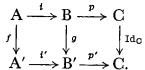
\includegraphics[keepaspectratio]{images/part002_08e8b4be.jpg}}

\begin{enumerate}
\def\labelenumi{(\roman{enumi})}
\setcounter{enumi}{3}
\tightlist
\item
  若 \(b \in \mathbf{B}\) 且 \(a' \in \mathbf{A}'\)，则
\end{enumerate}

\[
g (b) i ^ {\prime} \left(a ^ {\prime}\right) g (b) ^ {- 1} = i ^ {\prime} (\omega (b) a ^ {\prime}).
\]

\begin{enumerate}
\def\labelenumi{(\roman{enumi})}
\tightlist
\item
  对于 A 中的 \(a_{1}\)、\(a_{2}\)，在 B'' 中有
\end{enumerate}

\[
\begin{array}{r l} (f (a _ {1} ^ {- 1}), i (a _ {1})) (f (a _ {2} ^ {- 1}), i (a _ {2})) & = (f (a _ {1} ^ {- 1}) (\omega (a _ {1}) f (a _ {2} ^ {- 1})), i (a _ {1}) i (a _ {2})) \\ & = (f (a _ {1} ^ {- 1}) f (a _ {1} a _ {2} ^ {- 1} a _ {1} ^ {- 1}), i (a _ {1} a _ {2})) \\ & = (f ((a _ {1} a _ {2}) ^ {- 1}, i (a _ {1} a _ {2})) \end{array}
\]

因而 \(a \mapsto (f(a^{-1}), i(a))\)\(h\) 是从 \(A\) 到 \(B''\) 的同态 h。令 \(a \in A\)、\(a' \in A'\)、\(b \in B\)；则在 \(B''\) 中，

\[
\begin{array}{r l} b h (a) b ^ {- 1} & = b f (a ^ {- 1}) a b ^ {- 1} = (\omega (b) f (a ^ {- 1})) (b a b ^ {- 1}) \\ & = f (b a ^ {- 1} b ^ {- 1}) (b a b ^ {- 1}) = h (b a b ^ {- 1}) \\ a ^ {\prime} h (a) a ^ {\prime - 1} & = a ^ {\prime} f (a ^ {- 1}) a a ^ {\prime - 1} = a ^ {\prime} f (a ^ {- 1}) (\omega (a) a ^ {\prime - 1}) a \\ & = a ^ {\prime} f (a ^ {- 1}) f (a) a ^ {\prime - 1} f (a ^ {- 1}) a = h (a) \end{array}
\]

因而 \(h(A) = D\)\(B''\) 是 B'' 的正规子群。

\begin{enumerate}
\def\labelenumi{(\roman{enumi})}
\setcounter{enumi}{1}
\tightlist
\item
  对于 \(a \in A\)，
\end{enumerate}

\[
(p \circ q) (h (a)) = p (q (f (a ^ {- 1}) a)) = p (a) = e
\]

因而 \(p \circ q\) 在 D 上是平凡的。

\begin{enumerate}
\def\labelenumi{(\roman{enumi})}
\setcounter{enumi}{2}
\tightlist
\item
  设 \(a' \in A'\) 满足 \(i'(a') = e\)；则 \(a' \in D\)，因而存在 \(a \in A\) 使得 \(a' = f(a^{-1})a\)；这蕴含 \(a = e\)，从而 \(a' = e\)；故 \(i'\) 是单射。由于 \(p\) 和 \(q\) 是满射，\(p'\) 是满射。
\end{enumerate}

令 \(r\) 表示从 \(B''\) 到 \(B'\) 的典范态射。设 \(a' \in A'\)、\(b \in B\)，且 \(b' = r(a'b)\)。若 \(b' \in \operatorname{Im}(i')\)，则存在 \(a_1' \in A'\) 使得 \(b' = r(a_1')\)；于是存在 \(a \in A\) 使得 \(a'b = a_1'f(a^{-1})a\)，从而 \(b = a \in A\)，且

\[
p ^ {\prime} (b ^ {\prime}) = p (q (a ^ {\prime} b)) = p (b) = e;
\]

因此，\(\operatorname{Im}(i') \subset \operatorname{Ker}(p')\)。仍用 \(a', b, b'\) 表示上述对象，但假设 \(b' \in \operatorname{Ker}(p')\)；于是 \(e = p'(b') = p(q(a'b)) = p(b)\)，从而 \(b \in A\)，故

\[
b ^ {\prime} = r (a ^ {\prime} f (b) f (b ^ {- 1}) b) = r (a ^ {\prime} f (b)) \in \operatorname{Im} (i ^ {\prime});
\]

因此 \(\operatorname{Ker}(p') \subset \operatorname{Im}(i')\)。

若 \(a\in \mathbf{A}\)，则

\[
i ^ {\prime} (f (a)) = r (f (a)) = r (f (a) f \left(a ^ {- 1}\right) a) = r (a) = g (i (a)).
\]

若 \(b\in \mathbf{B}\)，则

\[
p ^ {\prime} (g (b)) = p (b)
\]

从而图 (4) 交换。

\begin{enumerate}
\def\labelenumi{(\roman{enumi})}
\setcounter{enumi}{3}
\tightlist
\item
  设 \(b \in \mathbf{B}\)、\(a' \in \mathbf{A}'\)。则
\end{enumerate}

\[
\begin{array}{r} g (b) i ^ {\prime} (a ^ {\prime}) g (b) ^ {- 1} = r (b) r (a ^ {\prime}) r (b) ^ {- 1} = r (b a ^ {\prime} b ^ {- 1}) \\ = r (\omega (b) a ^ {\prime}) = i ^ {\prime} (\omega (b) a ^ {\prime}). \end{array}
\]

命题 20. 设 G 是有限维实李群。

\begin{enumerate}
\def\labelenumi{(\roman{enumi})}
\item
  存在一个复李群 \(\tilde{\mathbf{G}}\) 和一个从 \(\mathbf{R}\) 到 \(\gamma\) 的 \(\mathbf{G}\)-解析态射 \(\tilde{\mathbf{G}}\)，具有如下性质：对于每个复李群 \(\mathbf{H}\) 以及每个从 \(\mathbf{R}\) 到 \(\phi\) 的 \(\mathbf{G}\)-解析态射 \(\mathbf{H}\)，存在唯一一个从 \(\mathbf{C}\) 到 \(\psi\) 的 \(\tilde{\mathbf{G}}\)-解析态射 \(\mathbf{H}\)，使得 \(\phi = \psi \circ \gamma\)。
\item
  若 \((\tilde{\mathbf{G}}', \gamma')\) 与 \((\tilde{\mathbf{G}}, \gamma)\) 具有相同性质，则存在唯一一个从 \(\theta\) 到 \(\tilde{\mathbf{G}}\) 的同构 \(\tilde{\mathbf{G}}'\)，使得 \(\theta \circ \gamma = \gamma'\)。
\item
  延拓 \(\mathbf{C}\) 的从 \(\mathrm{L}(\mathrm{G}) \otimes \mathbf{C}\) 到 \(\mathrm{L}(\tilde{\mathrm{G}})\) 的 \(\mathrm{L}(\gamma)\)-线性映射是满射；特别地，\(\dim_{\mathbf{C}}(\tilde{\mathbf{G}}) \leqslant \dim_{\mathbf{R}}(\mathrm{G})\)。
\end{enumerate}

断言 (ii) 是显然的。我们证明具有性质 (i) 和 (iii) 的有序对 \((\tilde{G},\gamma)\) 的存在性。

\begin{enumerate}
\def\labelenumi{(\alph{enumi})}
\tightlist
\item
  首先假设 \(G\) 连通。令 \(g = L(G)\)，\(g_{\mathbf{C}} = g \otimes_{\mathbf{R}} \mathbf{C}\) 为 \(g\) 的复化，令 \(S\)（分别地，\(S'\)）为李代数为 \(g\)（分别地，\(g_{\mathbf{C}}\)）的单连通实（分别地，复）李群，并令 \(\sigma\) 为唯一的从 \(\mathbf{R}\) 到 \(S\) 的 \(S'\)-解析态射，使得 \(L(\sigma)\) 是从 \(g\) 到 \(g_{\mathbf{C}}\) 的典范嵌入。令 \(\pi\) 为唯一的从 \(\mathbf{R}\) 到 \(S\) 的 \(G\)-解析态射，使得 \(L(\pi) = I d_{L(G)}\) 且 \(F = K e r \pi\)。
\end{enumerate}

\pandocbounded{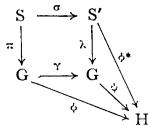
\includegraphics[keepaspectratio]{images/part002_6429af2f.jpg}}

对于每个复李群 H 以及每个从 G 到 H 的 R-解析态射 \(\phi\)，\(L(\phi): g \to L(H)\) 都有唯一的 C-线性延拓到 \(g_{C}\)，且此延拓形如 \(L(\phi^{*})\)，其中 \(\phi^{*}\) 是从 \(S'\) 到 H 的 C-解析态射。于是

\[
\mathrm{L} (\phi \circ \pi) = \mathrm{L} (\phi) \circ \mathrm{L} (\pi) = \mathrm{L} (\phi) = \mathrm{L} (\phi^ {*}) \circ \mathrm{L} (\sigma) = \mathrm{L} (\phi^ {*} \circ \sigma)
\]

因而 \(\phi \circ \pi = \phi^{*} \circ \sigma\)。所以 \(\phi^{*}(\sigma(F)) = \phi(\pi(F)) = \{e\}\)，从而

\[
\sigma (\mathrm{F}) \subset \operatorname{Ker} \phi^ {*}.
\]

令 P 为所有 \(\phi^{*}\) 变化时的 Ker \(\phi\) 的交。这是 \(S'\) 的正规李子群（第 2 号，命题 1 的推论 3）。令 \(\tilde{G} = S'/P\)，令 \(\lambda: \mathbf{S}' \to \tilde{\mathbf{G}}\) 为典范态射。于是 \(\sigma(\mathbf{F}) \subset \mathbf{P}\)，因而存在唯一一个从 \(\mathbf{R}\) 到 \(\gamma\) 的 \(\mathbf{G}\)-解析态射 \(\tilde{\mathbf{G}}\)，使得 \(\gamma \circ \pi = \lambda \circ \sigma\)。若 \(\psi: \tilde{\mathbf{G}} \to \mathbf{H}\) 表示由 \(\phi^*\) 在取商时导出的态射，则

\[
(\phi \circ \gamma) \circ \pi = \psi \circ (\lambda \circ \sigma) = \phi^ {*} \circ \sigma = \phi \circ \pi
\]

从而 \(\psi \circ \gamma = \phi\)。显然，\(\mathrm{L}(\psi)\)，进而 \(\psi\)，由等式 \(\psi \circ \gamma = \phi\) 唯一确定。因此我们证明了有序对 \((\tilde{G}, \gamma)\) 具有性质 (i) 和 (iii)。

\begin{enumerate}
\def\labelenumi{(\alph{enumi})}
\setcounter{enumi}{1}
\tightlist
\item
  现在转到一般情形。令 \(\mathbf{F}\) 为 \(\mathrm{G},\mathrm{M} = \mathrm{G} / \mathrm{F}\) 的单位分支，，令 \(i\colon \mathrm{F}\to \mathrm{G}\) 和 \(p\colon \mathrm{G}\rightarrow \mathrm{M}\) 为典范态射。我们将证明的部分 (a) 应用于 F。得到有序对 \((\tilde{\mathbf{F}},\delta)\)。对于所有 \(g\in \mathrm{G}\)，内自同构 Int \(g|\mathrm{F} = \omega '(g)\) 是 F 的自同构。由 \(\tilde{\mathbf{F}}\) 的泛性质，存在唯一一个复李群 \(\omega (g)\) 的自同构 \(\tilde{\mathbf{F}}\)，使得 \(\delta \circ \omega '(g) = \omega (g)\circ \delta\)。显然，\(\omega\) 是从 G 到 \(\operatorname {Aut}(\tilde{\mathbf{F}})\) 的态射。若 \(g\in \mathbf{G}\) 且 \(f\in \tilde{\mathbf{F}}\)，则
\end{enumerate}

\[
\delta (g f g ^ {- 1}) = (\delta \circ \omega^ {\prime} (g)) (f) = (\omega (g) \circ \delta) (f) = \omega (g) (\delta (f)).
\]

若 \(f \in \mathbf{F}\)，则 \(\delta \circ (\operatorname{Int}_{\mathbb{F}} f) = (\operatorname{Int}_{\tilde{\mathbb{F}}} \delta(f)) \circ \delta\)，且 \(\operatorname{Int}_{\tilde{\mathbb{F}}} \delta(f)\) 是复李群 \(\tilde{\mathbf{F}}\) 的自同构；故 \(\operatorname{Int}_{\tilde{\mathbb{F}}} \delta(f) = \omega(f)\)。

因此可应用引理 7，从而得到交换图

\[
\begin{array}{c} \mathrm{F} \xrightarrow {i} \mathrm{G} \xrightarrow {p} \mathrm{M} \\ \delta \Big \downarrow \qquad \qquad \qquad \gamma \Big \downarrow \qquad \qquad \Big \downarrow \mathrm{Id} \\ \tilde {\mathrm{F}} \xrightarrow {\tilde {i}} \tilde {\mathrm{G}} \xrightarrow {\tilde {p}} \mathrm{M}. \end{array}
\]

借助 \(\tilde{\mathbf{F}}\)，将 \(\tilde{\mathbf{G}}\) 识别为 \(\tilde{i}\) 的正规子群。群 \(\tilde{\mathbf{G}}\) 由 \(\tilde{\mathbf{F}}\) 和 \(\gamma (\mathbf{G})\) 生成；因此，由 \(\tilde{\mathbf{F}}\) 的元素定义的 \(\tilde{\mathbf{G}}\) 的自同构都是复李群结构的自同构。由 § 1，第 9 号，命题 18，\(\tilde{\mathbf{G}}\) 上存在唯一一个复李群结构，使得 \(\tilde{\mathbf{F}}\) 是 \(\tilde{\mathbf{G}}\) 的开李子群。以下 \(\tilde{\mathbf{G}}\) 均取此结构。由于 \(\delta\) 是 \(\mathbf{R}\)-解析的，\(\gamma\) 也是 \(\mathbf{R}\)-解析的。

有序对 \((\tilde{G},\gamma)\) 具有命题的性质 (iii)。我们证明它具有性质 (i)。设 H 是复李群，\(\phi\) 是从 G 到 H 的 R-解析态射。存在一个从 \(\eta\) 到 H 的 C-解析态射 \(\tilde{F}\)，使得 \(\eta \circ \delta = \phi |F\)。设 \(g\in G\)。映射

\[
f \mapsto \eta (\omega (g) f), \quad f \mapsto \phi (g) \eta (f) \phi (g) ^ {- 1}
\]

从 \(\tilde{\mathbf{F}}\) 到 \(\mathbf{H}\) 都是 \(\mathbf{C}\)-解析态射；它们在 \(\delta(\mathbf{F})\) 上一致，因为若 \(f' \in \mathbf{F}\)，则

\[
\begin{array}{r} \phi (g) \eta (\delta (f ^ {\prime})) \phi (g) ^ {- 1} = \phi (g) \phi (f ^ {\prime}) \phi (g) ^ {- 1} = \phi (g f ^ {\prime} g ^ {- 1}) \\ = \eta (\delta (g f ^ {\prime} g ^ {- 1})) = \eta (\omega (g) \delta (f ^ {\prime})); \end{array}
\]

因此对于所有 \(\eta (\omega (g)f) = \phi (g)\eta (f)\phi (g)^{-1}\) 和所有 \(g\in G\)，都有 \(f\in \tilde{\mathbf{F}}\)。若 \(\mathbf{G}'\) 表示关于 \(\mathbf{G}\) 的 \(\tilde{\mathbf{F}}\) 与 \(\omega\) 的半直积，则存在从群 \(\zeta\) 到 \(\mathbf{G}'\) 的态射 \(\mathrm{H}\)，它在 \(\phi\) 上与 \(\mathrm{G}\) 一致，在 \(\eta\) 上与 \(\tilde{\mathbf{F}}\) 一致。对于 \(f\in \mathbf{F}\)，

\[
\zeta (\delta (f ^ {- 1}) f) = \eta (\delta (f ^ {- 1})) \phi (f) = \phi (f ^ {- 1}) \phi (f) = e.
\]

因此 \(\zeta\) 在取商后定义出从 \(\psi\) 到 H 的态射 \(\tilde{\mathbf{G}}\)。于是 \(\psi \circ \gamma = \phi\) 且 \(\psi \circ \tilde{i} = \eta\)；后一个等式蕴含 \(\psi\) 是 C-解析的。

最后，设 \(\psi'\) 是从 \(\mathbf{C}\) 到 \(\tilde{\mathbf{G}}\) 的 \(\mathbf{H}\)-解析态射，满足 \(\phi = \psi' \circ \gamma\)。则

\[
\psi^ {\prime} \circ \tilde {i} \circ \delta = \psi^ {\prime} \circ \gamma \circ i = \phi \circ i = \psi \circ \tilde {i} \circ \delta
\]

因而 \(\psi' \circ \tilde{i} = \psi \circ \tilde{i}\)。由于 \(\tilde{G}\) 由 \(\tilde{i}(\tilde{\mathrm{F}})\) 和 \(\gamma(G)\) 生成，\(\psi' = \psi\)。

定义 4. \((\tilde{G},\gamma)\)，或简记为 \(\tilde{G}\)，称为 G 的泛复化。

注记。(1) 设 \((\tilde{\mathbf{G}},\gamma)\) 是 G 的泛复化。设 \(G_0\)（分别地，\(\tilde{G}_0\)）为 G（分别地，\(\tilde{G}\)）的单位分支。由命题 20 的证明，\((\tilde{G}_0,\gamma |G_0)\) 是 \(G_0\) 的泛复化，且复合态射

\[
\mathrm{G} \rightarrow \tilde {\mathrm{G}} \rightarrow \tilde {\mathrm{G}} / \tilde {\mathrm{G}} _ {0}
\]

在取商后定义出从 \(\mathbf{G} / \mathbf{G}_0\) 到 \(\tilde{\mathbf{G}} / \tilde{\mathbf{G}}_0\) 的同构。

\begin{enumerate}
\def\labelenumi{(\arabic{enumi})}
\setcounter{enumi}{1}
\tightlist
\item
  假设 G 单连通。令 \(g = L(G)\)，令 \(g_{c}\) 为 g 的复化，令 \(S'\) 为李代数为 \(g_{c}\) 的单连通复李群，令 \(\sigma\) 为从 G 到 \(S'\) 的态射，使得 \(L(\sigma)\) 是从 g 到 \(g_{c}\) 的典范嵌入。我们再次使用命题 20 的证明中部分 (a) 的记号。若 \(H = S'\) 且 \(\phi = \sigma\)，则 \(\phi^{*} = I d_{g}\)。因此 \((S', \sigma)\) 是 G 的泛复化。注意 \(\sigma\) 一般并非单射（练习 16）；然而由于 \(L(\sigma)\) 是单射，其核是离散的。另一方面，令 \(\theta\) 为由 g 定义的 \(g_{c}\) 的对合，令 \(\eta\)\(S'\) 为 S' 的底层实李群所对应的自同构；令 \(S'^{\eta}\)\(S'\) 为 S' 中在 \(\eta\)\(S'\) 下不变的点的集合；它是 S' 的实李子群，其李代数为 g（§3，第 8 号，命题 29 的推论 1）。由第 1 号、命题 1 的推论 1，\(\sigma(G)\)\(S'\) 是 S' 的李代数为 g 的实积分子群，因而 \(\sigma(G)\) 是 \(S'^{\eta}\) 的单位分支；特别地，\(\sigma(G)\)\(S'\) 是 S' 的实李子群。
\end{enumerate}

\section{超度量域上的李群}

本节假定赋值域 K 是超度量的且特征为 0。令 A 表示 K 的赋值环，m 表示 A 的极大理想，p 表示剩余域 A/m 的特征。若 K 是局部紧的，则 \(p \neq 0\)（交换代数，第 VI 章，§ 9，定理 1）。

\subsection{从李代数到李群}

命题 1. 设 G 是单位元为 e 的李群芽。G 中存在一个由 G 的李子群组成的 e 的开邻域基。

给 \(\mathrm{L}(\mathrm{G})\) 赋予一个与其拓扑相容的范数，并使得对 \(\| [x,y]\| \leqslant \| x\| \| y\|\) 中所有 \(x,y\) 都有 \(\mathrm{L}(\mathrm{G})\)。令 \(\mathrm{G}_1\) 为由 \(\mathrm{L}(\mathrm{G})\) 定义的李群。由 § 4，第 2 号，定理 2，G 与 \(\mathrm{G}_1\) 局部同构。因此只需应用 § 4，第 2 号，引理 3 (iii)。

定理 1. 设 \(\mathbf{L}\) 是完备可赋范李代数。存在一个李群 \(\mathbf{G}\)，使得 \(\mathbf{L}(\mathbf{G})\) 同构于 \(\mathbf{L}\)。任意两个这样的群都局部同构。

第一个断言已在 § 4，第 2 号，引理 3 中证明。第二个断言是 § 4，第 2 号，定理 2 的特例。

定理 2. 设 G 是李群，b 是 L(G) 的具有拓扑补空间的李子代数。存在 G 的李子群 H，使得 L(H) = b。若 H₁ 和 H₂ 是 G 的李子群，且 L(H₁) = L(H₂) = b，则 H₁ ∩ H₂ 在 H₁ 和 H₂ 中都是开集。

第一个断言由命题 1 和 §4，第 2 号，定理 3 得到。第二个断言是 §4，第 2 号，定理 3 的特例。

定理 3. 设 \(\mathbf{G}\) 和 \(\mathbf{H}\) 是李群，\(h\) 是从 \(\mathbf{L}(\mathbf{G})\) 到 \(\mathbf{L}(\mathbf{H})\) 的连续态射。

\begin{enumerate}
\def\labelenumi{(\roman{enumi})}
\item
  存在 \(\mathbf{G}'\) 的开子群 \(\mathbf{G}\) 以及从 \(\phi\) 到 \(\mathbf{G}'\) 的李群态射 \(\mathbf{H}\)，使得 \(h = \mathbf{L}(\phi)\)。
\item
  设 \(\mathbf{G}_1, \mathbf{G}_2\) 是 \(\mathbf{G}\) 的开子群，\(\phi_i\) 是从 \(\mathbf{G}_i\) 到 \(\mathbf{H}\) 的态射，且 \(h = \mathbf{L}(\phi_i)\)。则 \(\phi_1\) 与 \(\phi_2\) 在 \(\mathbf{G}\) 的某个开子群上相同。
\end{enumerate}

由命题 1，这由 § 4，第 1 号，定理 1 得到。

命题 2. 设 \(\mathbf{G}\) 是李群，\(\mathfrak{h}\) 是 \(\mathbf{L}(\mathbf{G})\) 的具有拓扑补空间的李子代数。下列条件等价：

\begin{enumerate}
\def\labelenumi{(\roman{enumi})}
\item
  存在 \(\mathbf{G}'\) 的开子群 \(\mathbf{G}\) 以及 \(\mathbf{H}\) 的正规李子群 \(\mathbf{G}'\)，使得 \(\mathrm{L(H)} = \mathfrak{h}\)。
\item
  \(\mathfrak{h}\) 是 \(\mathrm{L}(\mathrm{G})\) 的理想。
\end{enumerate}

若存在具有 (i) 中性质的 \(G'\)\(H\) 和 H，则由 § 3，第 12 号，命题 47，有 \(L(G') = L(G)\)，且 \(L(H)\) 是 \(L(G')\) 的理想。

假设 \(\mathfrak{h}\) 是 \(\mathrm{L}(\mathrm{G})\) 的理想。存在一个李群 \(\mathrm{F}\)，使得 \(\mathrm{L}(\mathrm{F}) = \mathrm{L}(\mathrm{G}) / \mathfrak{h}\)（定理 1）。令 h 为从 \(h\)\(\mathrm{L}(\mathrm{G})\) 到 \(\mathrm{L}(\mathrm{F})\) 的典范态射。由定理 3 (i)，存在 \(\mathrm{G}'\) 的开子群 \(\mathrm{G}\) 以及从 \(\phi\) 到 \(\mathrm{G}'\) 的李群态射 \(\mathrm{F}\)，使得 \(\mathrm{L}(\phi) = \mathrm{h}\)。由 § 3，第 8 号，\(\mathrm{H}\) 的核 \(\phi\) 是 \(\mathrm{G}'\) 的李子群，且 \(\mathrm{L}(\mathrm{H}) = \mathrm{Ker} \, \mathrm{L}(\phi) = \mathrm{Ker} \, h = \mathfrak{h}\)。最后，由于 ，\(\mathrm{H}\) 是 \(\mathrm{G}'\)\(\mathrm{H} = \mathrm{Ker} \, \phi\) 的正规子群。

\subsection{指数映射}

命题 3. 设 \(\mathbf{G}\) 是李群。存在 \(\phi\) 的指数映射 \(\mathbf{G}\)，具有如下性质：

\begin{enumerate}
\def\labelenumi{(\roman{enumi})}
\item
  \(\phi\) 定义在加法群 L(G) 的开子群 U 上；
\item
  \(\phi (\mathbf{U})\) 是 \(\mathbf{G}\) 的开子群，且 \(\phi\) 是从解析流形 \(\mathbf{U}\) 到解析流形 \(\phi (\mathbf{U})\) 的同构；
\item
  对所有 \(\phi(nx) = \phi(x)^n\) 和所有 \(x \in \mathbf{U}\)，都有 \(n \in \mathbf{Z}\)。
\end{enumerate}

给 \(\dot{\mathrm{L}}(\mathrm{G})\) 赋予一个与其拓扑相容的范数，并使得对 \(\| [x,y]\| \leqslant \| x\| \| y\|\) 中的 \(x,y\) 有 \(\mathrm{L}(\mathrm{G})\)。令 \(\mathbf{G}_1\) 为由 \(\mathrm{L}(\mathrm{G})\) 定义的李群。令 \(\psi = \mathrm{Id}_{\mathrm{G}_1}\)，它是 \(\mathbf{G}_1\) 的一个指数映射。对所有 \(\mu >0\)，令 \(\mathrm{L}_{\mu}\) 为满足 \(x\in \mathrm{L}(\mathrm{G})\) 的 \(\| x\| < \mu\) 的集合。于是，当 \(\mu\) 充分小时，\(\mathrm{L}_{\mu}\) 是加法群 \(\mathrm{L}(\mathrm{G}),\psi (\mathrm{L}_{\mu})\)\(\mathrm{G}_1\) 的开子群，\(\psi |\mathrm{L}_{\mu}\) 是 \(\mathrm{L}_{\mu}\) 的开子群（§ 4，第 2 号，引理 3），\(\psi (\mathrm{L}_{\mu})\) 是从解析流形 \(\psi (nx) = \psi (x)^n\) 到 \(x\in \mathrm{L}_{\mu}\) 的解析流形同构，并且对所有 \(n\in \mathbf{Z}\) 和所有 \(\mathrm{L}_{\mu}\)，有 \(\mathrm{L}(\mathrm{G})\)。\(\mu\) 构成  中 0 的邻域基。由定理 1，存在 \(\mathbf{G}'\) 以及 \(\mathbf{G}\) 的开子群 \(\psi (\mathrm{L}_{\mu})\)，使得  与 \(\mathbf{G}'\) 同构，从而得到命题。

命题 4. 设 G 是李群，\(\phi\) 是 G 的单射指数映射。假设 \(p > 0\)。对 L(G) 中所有 \(x, y\)，

\begin{enumerate}
\def\labelenumi{(\arabic{enumi})}
\tightlist
\item
\end{enumerate}

\[
x + y = \lim _ {n \rightarrow + \infty} p ^ {- n} \phi^ {- 1} (\phi (p ^ {n} x) \phi (p ^ {n} y))\tag{1}
\]

\[
[ x, y ] = \lim _ {n \rightarrow + \infty} p ^ {- 2 n} \phi^ {- 1} (\phi (p ^ {n} x) \phi (p ^ {n} y) \phi (- p ^ {n} x) \phi (- p ^ {n} y)).\tag{2}
\]

这些是 § 4，第 3 号，命题 4 的特例。

\subsection{标准群†}

若 \(\mathrm{S}(\mathbf{X}_{1},\mathbf{X}_{2},\ldots,\mathbf{X}_{n})\) 是系数在 A 中的形式幂级数，则对于 m 中的所有 \(x_{1},\ldots,x_{r}\)，级数 \(\mathrm{S}(x_{1},x_{2},\ldots,x_{r})\) 收敛。更确切地说，\(m\times m\times\cdots\times m\) 包含于 S 的绝对收敛域（可微与解析流形，R，4.1.3）。

定义 1. 设 \(r\) 是满足 \(\geqslant 0\)\(r\)\(\mathbf{K}\)\(G\) 的整数。K 上 r 维的标准群是具有下列性质的李群 G：

\begin{enumerate}
\def\labelenumi{(\roman{enumi})}
\item
  G 的底层解析流形是 m × m × · · · × m（r 个因子）；
\item
  存在一个以 \(\mathbf{F}\) 为系数、无常数项的关于 \(2r\) 个变量的形式幂级数 \(\mathbf{A}^r\)，使得对 G 中所有 \(x.y = \mathbf{F}(x,y)\)，都有 \(x,y\)\(\mathbf{G}\)。
\end{enumerate}

于是 0.0 = 0，从而 G 的单位元是 m × m · · · × m 的原点。
† 第 3、4 号的结果及其证明在 K 的特征为正时仍然成立。

将 L(G) 识别为 \(K^r\)。由 § 5，公式 (13)，L(G) 关于典范基的结构常数属于 A。在同一证明中，我们需要把 m × ⋯ × m 中的元素既看作 G 的元素，又看作 L(G) 的元素。

例。设 \(G = 1 + \mathbf{M}_{n}(m)\)，它是 \(\mathbf{M}_{n}(\mathbf{K})\) 的开子集。若 \(x \in G\)，则 det \(x \in 1 + m\)，因而 \(G \subset \mathbf{GL}(n, K)\)。显然 \(GG \subset G\)。若 \(x = 1 + y\)，其中 \(y \in \mathbf{M}_{n}(m)\)，则矩阵求逆的计算首先说明 \(x^{-1} \in \mathbf{M}_{n}(\mathbf{A})\)；若写作 \(x^{-1} = 1 + y'\)，则 \(y + y' + yy' = 0\)，从而 \(y' \in \mathbf{M}_{n}(m)\)，因此 \(x^{-1} \in G\)。所以 G 是 \(\mathbf{GL}(n, K)\) 的开子群。我们借助映射 \(m^{n^2}\) 将 G 与 \((\delta_{ij} + y_{ij}) \mapsto (y_{ij})\) 识别。显然 G 是标准群。

定理 4. 设 G 是有限维李群。G 存在一个开子群同构于标准群。

将 G 替换为与 G 的某个开子群同构的群后，问题归结为 G 是 \(K^{r}\) 的开子集，单位元为 0，且乘积 x.y 和逆元 \(x^{[-1]}\) 的坐标由下列公式给出：

\begin{enumerate}
\def\labelenumi{(\arabic{enumi})}
\setcounter{enumi}{2}
\tightlist
\item
\end{enumerate}

\[
(x. y) _ {i} = x _ {i} + y _ {i} + \sum_ {| \alpha | \geqslant 1, | \beta | \geqslant 1} c _ {\alpha \beta i} x ^ {\alpha} y ^ {\beta} (i = 1, 2, \dots , r)\tag{3}
\]

\[
(x ^ {[ - 1 ]}) _ {i} = - x _ {i} + \sum_ {| \alpha | > 1} d _ {\alpha i} x ^ {\alpha} \quad (i = 1, 2, \dots , r)\tag{4}
\]

令 \(x, y\)\(G\)\(\lambda \in K^*\)\(G\)，通过比为 \(G' = \lambda G\) 的位似将群运算从 G 搬到 \(\lambda\)。对于 G' 中的 \(x', y'\)\(G'\)，在 G' 中计算的乘积 \(x'.y'\) 和逆元 \(x'^{(-1)}\)\(G'\) 的坐标为

\[
(x ^ {\prime}. y ^ {\prime}) _ {i} = x _ {i} ^ {\prime} + y _ {i} ^ {\prime} + \sum_ {| \alpha | \geqslant 1, | \beta | \geqslant 1} c _ {\alpha \beta i} ^ {\prime} x ^ {\prime \alpha} y ^ {\prime \beta} (i = 1, 2, \dots , r)
\]

\[
(x ^ {\prime [ - 1 ]}) _ {i} = - x _ {i} ^ {\prime} + \sum_ {| \alpha | > 1} d _ {\alpha i} ^ {\prime} x ^ {\prime \alpha} \quad (i = 1, 2, \dots , r)
\]

其中

\[
c _ {\alpha \beta i} ^ {\prime} = \lambda^ {- | \alpha | - | \beta | + 1} c _ {\alpha \beta i}, \quad d _ {\alpha i} ^ {\prime} = \lambda^ {- | \alpha | + 1} d _ {\alpha i}.
\]

由于级数 (3) 和 (4) 收敛可知，当 \(|\lambda|\) 充分大时，对所有 \(\alpha, \beta, i\)，

\[
\left| c _ {\alpha \beta i} ^ {\prime} \right| \leqslant 1, \quad \left| d _ {\alpha i} ^ {\prime} \right| \leqslant 1
\]

即 \(c_{\alpha\beta i}^{\prime}\in A\) 且 \(d_{\alpha i}^{\prime}\in A\)；另一方面 \(G^{\prime}\supset m\times m\times\cdots\times m\)。于是 \(m\times m\times\cdots\times m\) 是 \(G^{\prime}\) 的开子群，且是标准群。

\subsection{标准群的滤过}

我们再次采用定义 1 的记号。选取一个数 \(a > 1\) 和 K 的实赋值 \(v\)\(\mathbf{K}\)，使得对所有 \(|x| = a^{-v(x)}\) 都有 \(x \in \mathbf{K}\)\(a\)（交换代数，第 VI 章，§6，命题 3）。若 a 是 A 的包含于 m 中的非零（因而是开的）理想，令 \(\mathrm{G}(a)\)\(a\) 表示坐标属于 a 的 G 中元素的集合。若 \(\lambda \in \mathbf{R}\)，令 \(a_{\lambda}\)（分别地，\(a_{\lambda}^{+}\)）表示满足 \(x \in \mathbf{K}\)（分别地，\(v(x) \geqslant \lambda\)）的 \(v(x) > \lambda\) 的集合；于是 \(a_0 = A\)，\(a_0^+ = m\)。对于 \(x = (x_1, \ldots, x_r) \in G\)，记

\[
\omega (x) = \inf (v (x _ {1}), \dots , v (x _ {r})).\tag{5}
\]

命题 5. 设 G 是标准群。

\begin{enumerate}
\def\labelenumi{(\roman{enumi})}
\item
  若 \(\mathfrak{a}\) 是包含于 \(\mathbf{A}\) 中的 \(\mathfrak{m}\) 的非零理想，则 \(\mathbf{G}(\mathfrak{a})\) 是 \(\mathbf{G}\) 的开正规子群。
\item
  当 \(\mathbf{G}(\mathfrak{a}_{\lambda})\) 时，\(\lambda > 0\)\(e\) 构成 \(\mathbf{G}\) 中 e 的邻域基。
\item
  假设 \(\mathfrak{a}_{\lambda} \subset \mathfrak{a}\)（当 \(\lambda \geqslant \lambda_0\) 时），并给 \(G(\mathfrak{a}) / G(\mathfrak{a}_{\lambda})\) 赋予离散拓扑（当 \(\lambda \geqslant \lambda_0\) 时）。则拓扑群 \(G(\mathfrak{a})\) 是各群 \(G(\mathfrak{a}) / G(\mathfrak{a}_{\lambda})\) 的逆极限。
\item
  设 \(\mathfrak{a},\mathfrak{b}\) 是包含于 \(\mathfrak{m}\) 中的 A 的非零理想，满足 \(\mathfrak{a} \supset \mathfrak{b} \supset \mathfrak{a}^2\)。从 G(a) 到 (a/b) × · · · × (a/b) 的映射 \(x \mapsto (x_1 \bmod \mathfrak{b}, \ldots, x_r \bmod \mathfrak{b})\) 在取商后定义出从 G(a)/G(b) 到加法群 (a/b) × · · · × (a/b) 的同构。
\end{enumerate}

若 \(x \in G\) 且 \(y \in G(a)\)\(x\)\(x.y\)\(a\)，则 x 和 x.y 的坐标模 a 相等。因此，对于 G 中的 \(x'\)、\(x''\)\(G\) 以及 G(a) 中的 \(y'\)、\(y''\)\(G(a)\)\(x'.x''\)\((x'.y')\)\((x''.y'')\)\(a\)，x'.x'' 与 (x'.y') . (x''.y'') 的坐标模 a 相等。这证明了 (i)。

\begin{enumerate}
\def\labelenumi{(\roman{enumi})}
\setcounter{enumi}{1}
\item
  显然。
\item
  由上可知，这由一般拓扑，第 III 章，§ 7，命题 2 得到。
\end{enumerate}

若 \(x \in G(a)\) 且 \(y \in G(a)\)\(x, y\)\(x + y\)，则由 § 5 的公式 (4)，x、y 的坐标与 x + y 的坐标模 \(G(a^2)\) 同余。这证明了 (iv)。

推论。假设 K 局部紧，令 \(q = \operatorname{Card}(\mathbf{A} / \mathfrak{m})\)。

\begin{enumerate}
\def\labelenumi{(\roman{enumi})}
\item
  若 \(a = m^{a}\) 且 \(b = m^{b}\)，其中 \(b \geqslant a \geqslant 1\)，则 \(\mathrm{G}(a)/\mathrm{G}(b)\) 是基数为 \(q^{r(b-a)}\) 的 p-群。
\item
  G(a) 是 p-群的逆极限。
\end{enumerate}

\(\mathrm{G}(\mathfrak{a})/\mathrm{G}(\mathfrak{b})\) 中元素的数目是 \((\mathrm{Card}(\mathfrak{a}/\mathfrak{b}))^{r}\)；若 \(b=a+1\)，则 a/b 是 A/m 上的一维向量空间，从而在此情形下得到 (i)；一般情形由对 b-a 作归纳得到。断言 (ii) 由 (i) 和命题 5 (iii) 得到。

命题 6. 设 \(\mathfrak{a}, \mathfrak{b}, \mathfrak{c}, \mathfrak{c}'\) 是包含于 \(\mathbf{A}\) 中的 \(\mathfrak{m}\) 的非零理想，满足

\[
\mathfrak {c} ^ {\prime} \subset \mathfrak {c}, \quad \mathfrak {a b} \subset \mathfrak {c}, \quad \mathfrak {a b} ^ {2} \subset \mathfrak {c} ^ {\prime}, \quad \mathfrak {a} ^ {2} \mathfrak {b} \subset \mathfrak {c} ^ {\prime}.
\]

若 \(x \in \mathrm{G}(\mathfrak{a})\) 且 \(y \in \mathrm{G}(\mathfrak{b})\)，则 \(x^{[-1]}y^{[-1]}x.y, x.y.x^{[-1]}y^{[-1]}\)、 和 \([x,y]\) 属于 \(\mathrm{G}(\mathfrak{c})\)，并且模 \(\mathrm{G}(\mathfrak{c}')\) 同余。

由 § 5，第 2 号，命题 1，存在 \(c_{\alpha \beta} \in \mathbf{A}^r\)，使得

\[
x ^ {[ - 1 ]}. y ^ {[ - 1 ]}. x. y - [ x, y ] = \sum_ {| \alpha | + | \beta | \geqslant 3} c _ {\alpha \beta} x ^ {\alpha} y ^ {\beta}.
\]

若 \(x = 0\) 或 \(y = 0\)，则 \(x^{[-1]}y^{[-1]}x.y - [x,y] = 0\)；因此 \(c_{0\beta} = c_{\alpha 0} = 0\)。另一方面，条件

\[
x \in \mathrm{G} (\mathfrak {a}), \quad y \in \mathrm{G} (\mathfrak {b}), \quad | \alpha | \geqslant 1, \quad | \beta | \geqslant 1, \quad | \alpha | + | \beta | \geqslant 3
\]

蕴含

\[
c _ {\alpha \beta} x ^ {\alpha} y ^ {\beta} \in \mathrm{G} (a ^ {2} b + a b ^ {2}) \subset \mathrm{G} (c ^ {\prime})
\]

因而 \(x^{[-1]} \cdot y^{[-1]}x \cdot y - [x, y] \in \mathrm{G}(\mathfrak{c}')\)。类似地可得

\[
x. y. x ^ {[ - 1 ]}. y ^ {[ - 1 ]} - [ x, y ] \in \mathrm{G} (\mathfrak {c} ^ {\prime}).
\]

最后，由 § 5，公式 (13)，\([x,y] \in G(\mathfrak{ab}) \subset G(\mathfrak{c})\)。

命题 7. (i) 族 \((\mathrm{G}(\mathfrak{a}_{\lambda}))\) 是 \(\mathbf{G}\) 上的中心滤过（第二章，§ 4，第 4 号，定义 2）。

\[
\text { (ii) } For \lambda \in \mathbf {R} _ {+} ^ {*}, G (a _ {\lambda}) = \{x \in G | \omega (x) \geqslant \lambda \}, G (a _ {\lambda} ^ {+}) = \{x \in G | \omega (x) > \lambda \}.
\]

\begin{enumerate}
\def\labelenumi{(\roman{enumi})}
\setcounter{enumi}{1}
\tightlist
\item
  显然。我们证明 (i)。显然 \(G(a_{\lambda}) = \bigcap_{\mu < \lambda} G(a_{\mu})\)，且 \(G = \bigcup_{\lambda > 0} G(a_{\lambda})\)。另一方面，若 \(x \in G(a_{\lambda})\) 且 \(y \in G(a_{\mu})\)，则
\end{enumerate}

\[
x ^ {[ - 1 ]}. y ^ {[ - 1 ]}. x. y \in G (a _ {\lambda + \mu})
\]

将命题 6 应用于 \(a = a_{\lambda}, b = a_{\mu}, c = c' = a_{\lambda + \mu}\) 得到。

由第二章，§ 4，第 4 号，我们可以构造与带中心滤过 \((G(a_\lambda))\) 的群 G 相联系的群 gr(G)。对所有 \(G_\lambda = G(a_\lambda)/G(a_\lambda^+)\) 写 \(\lambda > 0\)，得到 \(gr(G) = \bigoplus_{\lambda>0} G_\lambda\)。回忆一下（同上，命题 1），G 中的换位子使我们能够在 gr(G) 上定义括号，使 gr(G) 成为李代数，具体如下：若 \(x \in G_\lambda\) 且 \(y \in G_\mu\)，取 \(\bar{x}\) 在 \(G(a_\lambda)\) 中的一个代表元 x，以及 \(\bar{y}\) 在 \(G(a_\mu)\) 中的一个代表元 y；则 \([\bar{x},\bar{y}]\) 是 \(x^{[-1]}.y^{[-1]}.x.y \in G(a_{\lambda+\mu})\) 在 \(G_{\lambda+\mu}\) 中的类。由命题 6（取 \(a = a_\lambda, b = a_\mu, c = a_{\lambda+\mu}, c' = a_{\lambda+\mu}\)），可见 \([\bar{x},\bar{y}]\) 也是 \([x,y]\) 在 \(G_{\lambda+\mu}\) 中的类。因此，当把 G 看作由 \(K^r\)\(G(a_\lambda)\) 滤过的李子代数  时，相关分次李代数（第二章，§ 4，第 3 号）等于 gr(G)。

\subsection{标准群中的幂}

保留第 4 号的记号。

命题 8. 设 \(n \in \mathbf{Z}\)\(h_n\)，h＿n 是从 G 到 G 的映射 \(x \mapsto x^n\)\(G\)\(G\)\(a\)\(A\)\(m\)。设 a 是包含于 m 中的 A 的非零理想，且 \(n \notin a\)\(h_n|G(a)\)\(G(a)\)\(G(na)\)。则 h＿n 在 G(a) 上的限制是从解析流形 G(a) 到解析流形 G(na) 的同构。

由标准群的定义，\(h_n\) 在整个 G 上等\(G\)于一个系数在 A＾r 中的整级数。由\(A^r\) § 5，公式 (4)，此级数形如

\[
h _ {n} (x) = n x + \sum_ {| \alpha | \geqslant 2} a _ {\alpha} x ^ {\alpha}.
\]

因此，对于 \(x \in G\)，

\[
\begin{array}{r l} h _ {n} (n x) & = n ^ {2} \Big (x + \sum_ {| \alpha | \geqslant 2} a _ {\alpha} n ^ {| \alpha | - 2} x ^ {\alpha} \Big) \\ & = n ^ {2} \mathrm{S} (x) \end{array}
\]

其中我们记 \(\mathrm{S}(x)=x+\sum_{|\alpha| \geq 2} a_{\alpha} n^{|\alpha|-2} x^{\alpha}\)。此级数 \(\mathrm{S}(x)\) 定义了一个从 G 到 G 的解析映射，仍记为 S。由代数，第 IV 章，§6，命题 8，存在一个系数在  中的整级数 \(S'\)，使得 \(A^r\)\(\mathrm{S}'(\mathrm{S}(\mathrm{X}))=\mathrm{S}(\mathrm{S}'(\mathrm{X}))=\mathrm{X}\)。因此 S 是从解析流形 G 到自身的同构，并且对于 A 的任意包含于 m 中的非零理想 b，都有 \(\mathrm{S}(\mathrm{G}(\mathrm{b}))\subset\mathrm{G}(\mathrm{b}),\mathrm{S}'(\mathrm{G}(\mathrm{b}))\subset\mathrm{G}(\mathrm{b})\)、，从而

\[
\mathrm{S} (\mathrm{G} (\mathfrak {b})) = \mathrm{G} (\mathfrak {b}).
\]

由于 \(h_n(y) = n^2\mathrm{S}\left(\frac{1}{n} y\right)\) 对 \(y \in n\mathrm{G}\) 成立，可见 h＿n 在 \(h_n|n\mathrm{G}(\mathfrak{b})\)\(n\mathrm{G}(\mathfrak{b})\) 上的限制是从解析流形  到解析流形 \(n^2\mathrm{G}(\mathfrak{b})\) 的同构。但是，由于 \(n \notin \mathfrak{a}\)，对所有 \(|n| > |\lambda|\) 都有 \(\lambda \in \mathfrak{a}\)，从而 \(n^{-1}\mathfrak{a} \subset \mathfrak{m}\)，因此 \(\mathfrak{a}\) 具有形式 \(n\mathfrak{b}\)，其中 \(\mathfrak{b}\) 是包含于 \(\mathrm{A}\)\(\mathfrak{m}\) 中的 A 的非零理想。

推论。若 n 在 A 中可逆，则 h＿n 是从解析流形 G 到自身的同构。对于 A 的每个包含于 \(n\)\(h_n\)\(\mathfrak{a}\) 中的非零理想 \(\mathfrak{m}\)，都有 \(h_n(\mathrm{G}(\mathfrak{a})) = \mathrm{G}(\mathfrak{a})\)。对所有 \(x \in \mathrm{G}\)，都有 \(\omega(x^n) = \omega(x)\)。

这立即由命题 8 得到。

命题 9. 假设 \(p \neq 0\)。

\begin{enumerate}
\def\labelenumi{(\roman{enumi})}
\item
  设 \(\mathfrak{a},\mathfrak{b}\) 是 \(\mathbf{A}\) 的非零理想，满足 \(\mathfrak{b} \subset \mathfrak{a} \subset \mathfrak{m}\)。在群 \(\mathrm{G}(\mathfrak{a}) / \mathrm{G}(\mathfrak{b})\)\(p\) 中，每个元素的阶都是 p 的幂。
\item
  假设 \(v(p) = 1\)。若 \(x \in G\) 满足 \(\omega(x) > \frac{1}{p - 1}\)，则
\end{enumerate}

\[
\omega (x ^ {p}) = \omega (x) + 1.
\]

由 § 5，公式 (4)，对所有 \(x \in G\)，

\[
x ^ {p} = p x + \sum_ {| \alpha | \geqslant 2} c _ {\alpha} x ^ {\alpha}
\]

即使为了证明 (i)，也可以假设 \(c_{\alpha} \in A^{r}\)\(\alpha\)\(v(p) = 1\)。于是若 \(\omega(x) \geqslant 1\)，便有 \(\omega(x^{p}) \geqslant \omega(x) + 1\)，从而当 n 趋于 \(\omega(x^{p^{n}})\) 时 \(+\infty\)\(n\) 趋于 \(+\infty\)；这证明了 (i)。由于 \(\binom{p}{i}\)\(p\) 可被 p 整除，对于

\(1 \leqslant i \leqslant p - 1\)\(c_{\alpha} \in pA^{r}\)，§ 5，第 3 号，命题 2 说明，对于

\[
2 \leqslant | \alpha | \leqslant p - 1
\]

从而

\[
\omega \left(c _ {\alpha} x ^ {\alpha}\right) > \omega (p x) = \omega (x) + 1 \quad \text { for } 2 \leqslant | \alpha | \leqslant p - 1.
\]

另一方面，若 \(|\alpha| \geqslant p\)，则 \(\omega(c_{\alpha}x^{\alpha}) \geqslant p\omega(x)\)，而当 \(p\omega(x) > \omega(x) + 1\) 时，\(\omega(x) > \frac{1}{p - 1}\)。这证明了 (ii)。

\subsection{对数映射}

引理 1. 假设 \(p \neq 0\)\(G\)\(G_1\)\(G\)。设 G 是一个李群，G＿1 是 G 的一个同构于标准群的开子群，且 \(x \in G\)。下列条件等价：

\begin{enumerate}
\def\labelenumi{(\roman{enumi})}
\item
  x 的某个幂属于 \(x\)\(\mathbf{G}_1\)；
\item
  存在一个严格递增的整数序列 \((n_{i})\)，使得当 \(x^{n_{i}}\)\(e\) 趋于 \(i\) 时，\(+\infty\) 趋于 e。
  (ii) \(\Rightarrow\) (i)：显然。
  (i) \(\Rightarrow\) (ii)：假设 \(y = x^{m} \in G_{1}\)。由第 5 号的命题 9 (i)，当 n 趋于 \(y^{p^n}\) 时，\(e\)\(n\)\(+\infty\) 趋于 e，换言之，当 n 趋于 \(x^{mp^n}\) 时，\(e\)\(n\)\(+\infty\) 趋于 e。
\end{enumerate}

命题 10. 假设 \(p \neq 0\)\(G\)\(G_f\)。设 G 是有限维李群。令 G＿f 为满足存在严格递增的整数序列 \(x \in G\) 使得当 \((n_i)\) 趋于 \(x^{n_i}\)\(e\) 时 \(i\) 趋于 e 的 \(+\infty\) 的集合。

\begin{enumerate}
\def\labelenumi{(\roman{enumi})}
\item
  \(G_{f}\) 在 G 中是开的。
\item
  存在唯一一个从 \(\psi\) 到 L(G) 的映射 \(G_{f}\)，具有如下性质：
\end{enumerate}

\begin{enumerate}
\def\labelenumi{(\alph{enumi})}
\item
  \(\psi (x^n) = n\psi (x)\) 对所有 \(x\in \mathbf{G}_f\) 和所有 \(n\in \mathbf{Z}\) 成立；
\item
  存在 e 在 \(\mathbf{V}\) 中的一个开邻域 \(e\)\(\mathbf{G}\)，使得 \(\psi |\mathbf{V}\) 是一个单射指数映射的逆映射。
\end{enumerate}

\begin{enumerate}
\def\labelenumi{(\roman{enumi})}
\setcounter{enumi}{2}
\tightlist
\item
  映射 \(\psi\) 是解析的。
\end{enumerate}

存在 G 的一个开子群同\(\mathbf{G}\)构于标准群（第 3 号，定理 4）。断言 (i) 随即由引理 1 得到。

令 U 是 L(G) 的一个开子群，\(\phi\colon\mathrm{U}\to\phi(\mathrm{U})\) 是 G 的一个指数映射，具有第 2 号命题 3 的性质。可以假设 U 足够小，使得 \(\phi(\mathrm{U})\subset\mathrm{G}_{f}\)。令 \(x\in\mathrm{G}_{f}\)。存在 \(m\in\mathbf{Z}-\{0\}\)，使得 \(x^{m}\in\phi(\mathrm{U})\)。元素 \(\frac{1}{m}\phi^{-1}(x^{m})\)\(m\) 不依赖于 m 的选择。事实上，若 \(m'\in\mathbf{Z}\) 使得 \(x^{m'}\in\phi(\mathrm{U})\)，则 \(x^{mm'}\in\phi(\mathrm{U})\)，并且

\[
m ^ {\prime} \phi^ {- 1} (x ^ {m}) = \phi^ {- 1} (x ^ {m m ^ {\prime}}) = m \phi^ {- 1} (x ^ {m ^ {\prime}}),
\]

令 \(\psi(x) = \frac{1}{m}\phi^{-1}(x^m)\)。则 \(\psi|\phi(U) = \phi^{-1}\)。另一方面，若 \(n \in \mathbf{Z}\)，则

\[
\psi (x ^ {n}) = \frac {1}{m} \phi^ {- 1} (x ^ {n m}) = \frac {n}{m} \phi^ {- 1} (x ^ {m}) = n \psi (x).
\]

因此 \(\psi\)\(x\) 具有命题的性质 (a) 和 (b)。在 x 的某个邻域内，\(\psi\) 由映射 \(x \mapsto x^m\)、\(y \mapsto \phi^{-1}(y)\) 和 \(z \mapsto \frac{1}{m} z\) 复合而成；故 \(\psi\) 在 \(G_f\) 上是解析的。

最后，设 \(\psi'\) 是从 \(G_f\) 到 L(G) 的映射，\(e\) 是 \(G_f\) 中 e 的一个邻域，满足对于 \(\psi'(x^n) = n\psi'(x)\) 和 \(x \in G_f\) 有 \(n \in \mathbf{Z}\)，且 \(\psi'|V'\) 是一个单射指数映射的逆映射。于是 \(\psi\) 与 \(\psi'\) 在 e 的某个邻域 W 上一致。若 \(e\)\(x \in G_f\)，则存在 \(n \in \mathbf{Z}\) 使得 \(x^n \in W\)。于是

\[
n \psi^ {\prime} (x) = \psi^ {\prime} (x ^ {n}) = \psi (x ^ {n}) = n \psi (x)
\]

从而 \(\psi = \psi'\)。

定义 2. 命题 10 的映射 \(\psi\) 称为 G 的对数映射，记作 \(\log_{\mathbb{G}}\)，或简记为 log。

命题 11. 假设 \(p \neq 0\)。设 x、y 是 G＿f 中的两个可交换元素。则 xy \(x, y\)\(G_f\)\(xy \in G_f\) 且 \(\log(xy) = \log x + \log y\)。

xy \(xy \in G_f\)\(U\)\(L(G)\)\(\phi: U \to \phi(U)\)\(G\)\(U\) 这一事实由引理 1 得到。令 U 是加法群 L(G) 的一个开子群，\(\log(\phi(U))\) 是 G 的一个指数映射，具有第 2 号命题 3 的性质；可以假设 U 足够小，使得 \(\phi\) 是 \(n \in \mathbf{Z} - \{0\}\) 的逆映射。选取适当的 \(x^n \in \phi(U)\)，使得 \(y^n \in \phi(U)\)、\(u = \log x^n\)。令 \(v = \log y^n\)、\(x^n = \phi(u)\)，于是 \(y^n = \phi(v)\)、\([u,v] = 0\)。由公式 (2)，\(\phi(\lambda(u + v)) = \phi(\lambda u)\phi(\lambda v)\)。于是由 Hausdorff 公式，当 \(|\lambda|\)\(i\) 充分小时，；因而对于每个充分大的整数 i，

\[
\phi (p ^ {i} (u + v)) = \phi (p ^ {i} u) \phi (p ^ {i} v)
\]

即

\[
p ^ {i} (\log x ^ {n} + \log y ^ {n}) = \log (x ^ {n p ^ {i}} y ^ {n p ^ {i}})
\]

或

\[
n p ^ {i} (\log x + \log y) = n p ^ {i} \log (x y).
\]

命题 12. 假设 \(p \neq 0\)。设 \(x \in G_f\)。下列条件等价：

\begin{enumerate}
\def\labelenumi{(\roman{enumi})}
\item
  \(\log x = 0;\)
\item
  x 在 G 中是有限阶的。
\end{enumerate}

若存在整数 \(n > 0\) 使得 \(x^n = e\)，则

\[
n \log x = \log x ^ {n} = 0,
\]

若 \(\log x = 0\)\(\log x = 0\)，令 \(\mathrm{V}\)\(e\) 为 \(\mathbf{G}_f\) 中 e 的一个邻域，使得 \(\log |\mathrm{V}\) 是一个单射指数映射的逆映射。存在整数 \(n > 0\) 使得 \(x^n \in \mathrm{V}\)；等式 \(\log x^n = 0\) 蕴含 \(x^n = e\)。

命题 13. 假设 \(p \neq 0\)\(G\)。若 G 是紧群或标准群，则 \(G_f = G\)。

若 G 是标准群，只需应用引理 1。假设 G 是紧群。设 \(x \in G\)，V 是 G 中 e 的一个邻域。令 y 为序列 \(e\)\(y\)\((x^n)_{n \geqslant 0}\) 的一个聚点。对于每个 \(n > 0\)，存在两个整数 \(n_1, n_2\)，使得 \(n_1 \geqslant 2n_2 \geqslant n\)，且 \(x^{n_1} \in y\mathrm{V}, x^{n_2} \in y\mathrm{V}\)\(x^{n_1 - n_2} \in V^{-1}\mathrm{V}\)、，从而 ，并且 \(n_1 - n_2 \geqslant n\)。因此 \(x \in G_f\)。

推论。假设 K 局部紧。则 \(G_{f}\) 是 G 的紧子群的并。

令 \(x \in G\)\(x\)\(G\)。若 x 属于 G 的某个紧子群，则 \(x \in G_f\)（命题 13）。假设 \(x \in G_f\)\(K\)。由于 K 局部紧，G 存在一个紧的开子群 \(G_1\)\(G\)。于是存在整数 \(m > 0\)，使得 \(x^m \in G_1\)。由 \(G_2\) 生成的闭子群 \(x^m\) 包含于 \(G_1\)\(x\)，因而是紧的。于是 x 与 \(G_2\) 的元素交换，从而 \(G_2 \cup xG_2 \cup \cdots \cup x^{m-1}G_2\)\(G\)\(x\) 是 G 的包含 x 的紧子群。

例。假设 K 局部紧。令 U 为 A 的可逆元素的集合；它是李群 K* 的紧开子群。由命题 13，\(U \subset (\mathbf{K}^{*})_{f}\)；另一方面，若 \(x \in K^{*}\) 且 \(x \notin U\)，则当 n 趋于 \(x^{n}\) 时 \(+\infty\) 趋于 0，或者当 n 趋于 \(x^{n}\) 时 \(-\infty\) 趋于 0；因此 \(U = (\mathbf{K}^{*})_{f}\)。函数 \(\log_{K^{*}}\) 在 \(U_{f}\) 上有定义且解析，取值于 \(L(\mathbf{K}^{*}) = \mathbf{K}\)，并满足对 U 中所有 x、y，\(\log_{\mathbf{K}^{*}}(xy) = \log_{\mathbf{K}^{*}}(x) + \log_{\mathbf{K}^{*}}(y)\)；U 中满足 \(\log_{\mathbf{K}^{*}}(x) = 0\) 的元素 x 正是 K 的单位根。

我们再次采用第 3、4、5 号的记号。

命题 14. 假设 \(p \neq 0\)，且 \(v\) 选取为满足 \(v(p) = 1\)\(G\)\(E(X)\)\(L(X)\)\(G\)\(G\)。设 G 是标准群，E(X)（分别地，L(X)）是 G 的指数函数（分别地，对数函数）在 0 点的整级数展开。

\begin{enumerate}
\def\labelenumi{(\roman{enumi})}
\item
  E 的绝对收敛域（可微与解析流形，R，4.1.3）包含集合 \(\Delta\)，其中 \(x \in G\) 满足 \(\omega(x) > \frac{1}{p - 1}\)。令 \(\mathbf{E}'\) 表示由该级数在 \(\Delta\) 上定义的映射。则 \(\mathbf{E}'\) 是 G 的指数映射，且是从流形 \(\Delta\) 到自身的同构。
\item
  L 的绝对收敛域包含 G。令 L' 表示由该级数在 G 上定义的映射。则 L' 是 G 的对数映射，且 L' 在 \(\Delta\) 上的限制是 E' 的逆映射。
\item
  映射 \(\mathbf{E}'\) 在带 Hausdorff 法则的 \(\Delta\) 上是同构，并且其像为 \(\Delta\) 的子群 \(\mathbf{G}\)。
\end{enumerate}

采用 § 5，第 3、4 号的记号，有 \(E = \sum_{m \geqslant 1} \frac{\psi_{m,m}}{m!}\)（§ 5，第 4 号，命题 3）。由于系数 \(c_{\alpha\beta\gamma}\) 属于 A，\(\|\psi_{m,m}\| \leqslant 1\)（可微与解析流形，R，附录）。假定 \(K^{r}\) 采用范数

\[
\left\| \left(\lambda_ {1}, \dots , \lambda_ {r}\right) \right\| = \sup \left(\left| \lambda_ {1} \right|, \dots , \left| \lambda_ {r} \right|\right).
\]

由第二章，§ 8，第 1 号，引理 1，有 \(v(m!) \leqslant \frac{m - 1}{p - 1}\)。若 \(\omega(x) > \frac{1}{p - 1}\)，则可见当 m 趋于无穷时，\(m\omega(x) - v(m!)\) 趋于 \(+\infty\)\(m\)，从而

\[
\left\| \frac {\psi_ {m , m}}{m !} \right\| \| x \| ^ {m} \leqslant \frac {1}{| m ! |} \| x \| ^ {m}
\]

当 m 趋于  时，它趋于 0，并且

\[
\omega \left(\frac {\psi_ {m , m} (x)}{m !}\right) > \frac {m}{p - 1} - \frac {m - 1}{p - 1} = \frac {1}{p - 1} \quad \text { for } m \geqslant 1.
\]

因此 \(\Delta\) 包含于 E 的绝对收敛域，且 \(\mathrm{E}'(\Delta) \subset \Delta\)。显然，\(\mathrm{E}'\) 是一个指数映射。

若 \(L_{m}\)\(L\)\(m\) 表示 L 的 m 次齐次分量，则 §5，第 4 号，命题 3 说明，\(L_{m}\) 的每个系数都具有如下形式

\[
a _ {1} + \frac {1}{2} a _ {2} + \dots + \frac {1}{m} a _ {m}
\]

其中 \(a_1, a_2, \ldots, a_m\) 属于 A；但是

\[
\inf \left(v (1), v \left(\frac {1}{2}\right), \dots , v \left(\frac {1}{m}\right)\right) = o (\log m) \quad \text { as   } m \text {   tends   to   } + \infty
\]

且

\[
\inf \left(v (1), v \left(\frac {1}{2}\right), \dots , v \left(\frac {1}{m}\right)\right) \geqslant v \left(\frac {1}{m !}\right) \geqslant - \frac {m - 1}{p - 1}.
\]

因此，若 \(\omega(x) > 0\)，则 \(\|L_m\|. \|x\|^m\)\(m\) 当 m 趋于  \(+\infty\) 时趋于 0，所以 G 包含于 L 的绝对收敛域。另一方面，若 \(\omega(x) > \frac{m}{p-1}\)，则当 \(\omega(L_m(x)) > \frac{m}{p-1} - \frac{m-1}{p-1} = \frac{1}{p-1}\) 时，\(m \geqslant 1\)，从而 \(L'(\Delta) \subset \Delta\)。

由于形式幂级数 \(\mathrm{L}(\mathrm{E}(\mathrm{X}))\) 和 \(\mathrm{E}(\mathrm{L}(\mathrm{X}))\) 都等于 \(\mathbf{X}\)，可微与解析流形，\(\mathbf{R}\)，4.1.5 说明

\[
\mathrm{L} ^ {\prime} (\mathrm{E} ^ {\prime} (x)) = \mathrm{E} ^ {\prime} (\mathrm{L} ^ {\prime} (x)) = x
\]

对 \(x \in \Delta\)。因此 \(E'\) 是从流形 \(\Delta\) 到自身的同构，其逆同构是 \(L'\) 在 \(\Delta\) 上的限制。

\(\mathrm{L}(\mathrm{X}^{[n]}) = n\tilde{\mathrm{L}}(\mathrm{X})\) 对于整数 \(n\) 大于 \(> 0\) 成立（参见 § 5，第 4 号）。由于 \(G\) 以及 \(L\) 都包含于 \(X^{[n]}\) 的绝对收敛域，因而对所有 \(L'(x^n) = nL'(x)\)，有 \(x \in G\)。关系 \(L'| \Delta = E'^{-1}\) 蕴含，当 \(L'(x^n) = \log x^n\) 足够大时 \(n\)。所以 \(L'(x) = \log x\)。至此已经证明 (i) 和 (ii)。

令 \(H = \sum_{r,s \geq 0} H_{r,s}\) 为 Hausdorff 形式幂级数，h 为相对于 L(G) 的 Hausdorff 函数。\(\tilde{H}\) 的绝对收敛域包含 \(\Delta \times \Delta\)\(h\)，且 h 定义在 \(\Delta \times \Delta\) 上（第二章，§ 8，命题 2）。于是

\[
\mathrm{E} ^ {\prime} (x) \mathrm{E} ^ {\prime} (y) = \mathrm{E} ^ {\prime} (h (x, y))
\]

当 \(x, y\) 充分接近 0 时（§ 4，定理 4 (v)）。因此，按照第 3 号定义 1 的记号，形式幂级数 \(\mathbf{F}(\mathrm{E}(\mathbf{X}), \mathrm{E}(\mathbf{Y}))\) 和 \(\mathrm{E}(\mathrm{H}(\mathbf{X}, \mathbf{Y}))\) 相等。设 \(x, y\) 是 \(\Delta\) 的元素。于是

\[
\begin{array}{l} \sup _ {m} \left\| \frac {\psi_ {m , m}}{m !} \right\| (\sup \| x \|, \| y \|) ^ {m} <   1 \\ \sup _ {r, s} \| H _ {r, s} \| \| x \| ^ {r} \| y \| ^ {s} <   | p | ^ {1 / (p - 1)} \end{array}
\]

由第二章，§8，公式 (14)，以及可微与解析流形，R，4.1.5，\(\mathrm{E}'(x)\mathrm{E}'(y)\) 是将 \(x\) 代入 X、将 \(y\) 代入 Y 后得到的，而

\[
\mathrm{F} (\mathrm{E} (\mathrm{X}), \mathrm{E} (\mathrm{Y}))
\]

且 \(\mathrm{E}'(h(x,y))\) 是将 \(x\) 代入 \(\mathbf{X}\)、将 \(y\) 代入 \(\mathbf{Y}\) 后在 \(\mathrm{E}(\mathrm{H}(\mathbf{X},\mathbf{Y}))\) 中得到的。因此 \(\mathrm{E}'(x)\mathrm{E}'(y) = \mathrm{E}'(h(x,y))\)。

\section{\texorpdfstring{R 与 \(\mathbf{Q}_p\) 上的李群}{R 与 \textbackslash mathbf\{Q\}\_p 上的李群}}

\subsection{连续态射}

定理 1. 设 G 和 H 是在 R 或 \(Q_{p}\) 上的两个李群芽。设 f 是从 G 到 H 的连续态射。则 f 是解析的。

给 \(\mathrm{L}(\mathrm{G})\) 和 \(\mathrm{L}(\mathrm{H})\) 赋予定义其拓扑的范数，并使得对任意 \(\| [x,y]\| \leqslant \| x\| \| y\|\) 都有 \(x,y\)。存在 \(\mathrm{L}(\mathrm{G})\) 中以 0 为中心的开球 V，以及定义在 \(\phi\) 上的 \(\mathbf{G}\) 的指数映射 \(\mathbf{V}\)，满足：(1) \(\phi (\mathbf{V})\)\(e\) 是 G 中 e 的开邻域；(2) \(\phi\) 是从解析流形 V 到解析流形 \(\phi (\mathbf{V})\) 的同构；(3) 对所有 \(\phi (nx) = \phi (x)^n\) 和所有 \(x\in V\)，只要 \(n\in \mathbf{Z}\)，就有 \(nx\in V\)。对 H 类似地定义 W 和 \(\psi\)。必要时缩小 V，可设 \(f(\phi (\mathrm{V}))\subset \psi (\mathrm{W})\)。于是 \(g = \psi^{-1}\circ f\circ \phi\) 是从 V 到 W 的连续映射。

我们证明

\[
(x \in \mathrm{V}, \lambda \in \mathbf {Q} \text {   and   } \lambda x \in \mathrm{V}) \Rightarrow g (\lambda x) = \lambda g (x).\tag{1}
\]

可假设 \(\lambda \neq 0\)。写成 \(\lambda = \frac{r}{q}\)，其中 \(r, q\) 属于 \(\mathbf{Z} - \{0\}\)。令 \(y = \frac{r}{q} x\)。

若 \(\mathbf{K} = \mathbf{R}\)，记 \(z = \frac{x}{q} = \frac{y}{r} \in \mathrm{V}\)。于是 \(x = qz, y = rz\)、，从而

\[
g (x) = \psi^ {- 1} (f (\phi (q z))) = \psi^ {- 1} (f (\phi (z) ^ {q})) = \psi^ {- 1} (f (\phi (z)) ^ {q}).
\]

我们证明 \(\psi^{-1}(f(\phi(z))^q) = q\psi^{-1}(f(\phi(z))) = qg(z)\)。只需验证：若 \(u \in \psi(W)\) 且 \(u^q \in \psi(W)\)，则 \(\psi^{-1}(u^q) = q\psi^{-1}(u)\)；但若 \(u = \psi(v)\)、\(u^q = \psi(v')\)，则 \(v'/q \in W\)，且 \((\psi(v'/q))^q = u^q\)，从而 \(\psi(v'/q) = u = \psi(v)\)，所以 \(v' = qv\)。

同理，\(g(y) = rg(z)\)，从而 (1)。

若 \(\mathbf{K} = \mathbf{Q}_p\)，记 \(z = rx = qy \in \mathrm{V}\)，从而 \(g(z) = rg(x) = qg(y)\)，再次得到 (1)。

由于 \(\mathbf{Q}\) 在 K 中稠密，(1) 蕴含

\[
(x \in \mathrm{V}, \lambda \in \mathrm{K} \text {   and   } \lambda x \in \mathrm{V}) \Rightarrow g (\lambda x) = \lambda g (x).\tag{2}
\]

令 \(x \in L(G)\)，并令 \(\lambda, \lambda'\) 为 \(K^*\) 中的元素，使得 \(\lambda x \in V, \lambda' x \in V\)。则

\[
g (\lambda^ {\prime} x) = g \left(\frac {\lambda^ {\prime}}{\lambda} \lambda x\right) = \frac {\lambda^ {\prime}}{\lambda} g (\lambda x)
\]

由 (2)，可得 \(\frac{1}{\lambda} g(\lambda x) = \frac{1}{\lambda'} g(\lambda' x)\)\(h\)\(g\)。因此，g 到 \(\mathrm{L}(G)\) 的延拓 h 定义为：对于满足 \(h(x) = \frac{1}{\lambda} g(\lambda x)\) 的所有 \(\lambda\)，令 \(\lambda x \in \mathrm{V}\)\(h\)。显然 h 连续。我们证明

\[
(x \in \mathrm{L} (\mathrm{G}) \text {   and   } \lambda \in \mathrm{K}) \Rightarrow h (\lambda x) = \lambda h (x).\tag{3}
\]

令 \(\lambda' \in \mathbf{K}^*\)，使得 \(\lambda' x \in V\) 且 \(\lambda' \lambda x \in V\)。则

\[
h (\lambda x) = \frac {1}{\lambda^ {\prime}} g \left(\lambda^ {\prime} \lambda x\right) = \frac {1}{\lambda^ {\prime}} \lambda g \left(\lambda^ {\prime} x\right) = \lambda \frac {1}{\lambda^ {\prime}} g \left(\lambda^ {\prime} x\right) = \lambda h (x).
\]

令 \(x, y\) 属于 L(G)。则由 § 4，第 3 号，命题 4，

\[
\begin{array}{r l} h (x) + h (y) & = \lim _ {\lambda \in \mathbf {K} ^ {*},   \lambda \to 0} \lambda^ {- 1} \psi^ {- 1} (\psi (\lambda h (x)) \psi (\lambda h (y))) \\ & = \lim _ {\lambda \in \mathbf {K} ^ {*},   \lambda \to 0} \lambda^ {- 1} \psi^ {- 1} (\psi (h (\lambda x)) \psi (h (\lambda y))). \end{array}
\]

当 \(|\lambda|\) 充分小时，\(\lambda x \in V\) 且 \(\lambda y \in V\)，因而上式等于

\[
\begin{array}{r l} & \lim _ {\lambda \in \mathbf {K} ^ {*}, \lambda \to 0} \lambda^ {- 1} \psi^ {- 1} (f (\phi (\lambda x)) f (\phi (\lambda y))) \\ = & \lim _ {\lambda \in \mathbf {K} ^ {*}, \lambda \to 0} \lambda^ {- 1} (\psi^ {- 1} \circ f) (\phi (\lambda x) \phi (\lambda y)) \\ = & \lim _ {\lambda \in \mathbf {K} ^ {*}, \lambda \to 0} \lambda^ {- 1} g (\phi^ {- 1} (\phi (\lambda x) \phi (\lambda y))) \\ = & \lim _ {\lambda \in \mathbf {K} ^ {*}, \lambda \to 0} h (\lambda^ {- 1} \phi^ {- 1} (\phi (\lambda x) \phi (\lambda y))) \\ = & h (\lim _ {\lambda \in \mathbf {K} ^ {*}, \lambda \to 0} \lambda^ {- 1} \phi^ {- 1} (\phi (\lambda x) \phi (\lambda y))) \\ = & h (x + y). \end{array}
\]

因此 h 连续且线性，从而 \(h\)\(g = h|\mathrm{V}\)\(f\) 是解析的，继而 f 在 \(\phi(\mathrm{V})\)\(f\) 上解析，因而 f 是解析的（§ 1，第 10 号）。

推论 1. 设 G 是拓扑群。G 上至多存在一个与 G 的拓扑群结构相容的、在 R（分别地，\(Q_{p}\)）上的解析流形结构。

这立即由定理 1 得到。

定义 1. 若拓扑群 G 上存在一个与其拓扑相容的 R（分别地，p 进）李群结构，则称 G 为实（分别地，p 进）李群。

该结构于是唯一，我们可以谈论此类群的维数。若 G 和 H 是两个这样的群，则从 G 到 H 的每个连续态射都是解析的。

推论 2. 设 G 是拓扑群，V 是 e 的一个开邻域。假设 V 具有一个解析流形结构，使其成为实（分别地，p 进）李群芽。则 G 是实（分别地，p 进）李群。

设 \(g \in G\)。存在 G 中 e 的一个开邻域 \(V'\)\(e\)\(G\)，使得 \(V' \cup gV'g^{-1} \subset V\)。从 \(v \mapsto gvg^{-1}\) 到 V 的映射 \(V'\)\(V\) 是连续的，因而是从李群芽 \(V'\)\(V\) 到李群芽 V 的解析态射。因此只需应用 § 1，第 9 号，命题 18。

注记。(1) 若将 \(\mathbf{R}\)（分别地，\(\mathbf{Q}_p\)）替换为 \(\mathbf{C}\)，则定理 1 及其推论不再成立（练习 1）。

\begin{enumerate}
\def\labelenumi{(\arabic{enumi})}
\setcounter{enumi}{1}
\tightlist
\item
设 G 是拓扑群。可以证明†下列条件等价：(a) G 是有限维实李群；(b) G 是局部紧的，且存在 e 的一个邻域，其中不含 \{\} 以外的子群；(c) e 存在一个开邻域，同胚于空间 \(R^{n}\) 的开球。（一个容易得多的结果参见练习 6。）
\end{enumerate}
† 例如见 D. Montgomery 和 L. Zippin，《拓扑变换群》，纯粹与应用数学 Interscience 专论，第 1 号，Interscience 出版社，纽约，1955（尤其是第 169 和 184 页）。

命题 1. 设 \(G, G'\)\(f\)\(G\) 是拓扑群，f 是从 G 到 \(G'\) 的连续态射。假设下列三种情形之一成立：

\begin{enumerate}
\def\labelenumi{(\alph{enumi})}
\item
  G 是实李群，而 \(\mathbf{G}'\) 是 \(p\) 进李群；
\item
  G 是 p 进李群，而 \(G'\) 是实李群；
\item
  G 是 p 进李群，而 \(G'\) 是 \(p'\) 进李群，且 \(p \neq p'\)。
\end{enumerate}

则 \(f\)f 是局部常值的。

情形 (a)。令 \(G_0\)\(G\) 为 G 的单位分支。则 \(f(G_0)\) 是 \(G'\) 的连通子群，因而 \(f(G_0) = \{e\}\)，且 \(G_0\)\(G\) 在 G 中是开的。

情形 (b)。令 \(V'\) 为 \(G'\) 中 e 的一个邻域，使得包含于 \(G'\) 中的 \(V'\) 的每个子群都退化为 \(\{e\}\)（§4，第 2 号，定理 2 的推论 1）。存在 G 中 e 的一个邻域 V，使得 \(f(V) \subset V'\)。于是存在 G 的开子群 \(G_{1}\)，使得 \(G_{1} \subset V\)（§7，第 1 号，命题 1）。因此 \(f(G_{1}) = \{e\}\)。

情形 (c)。由 § 7，定理 4 及命题 8 的推论，存在  中 e 的一个邻域 \(\mathbf{V}'\)，使得对所有 \(e\)\(\mathbf{G}'\)\(x' \in \mathbf{V}' - \{e\}\)，当 n 趋于 \(x'^{p^n}\) 时 \(e\)\(n\)\(+\infty\) 不趋于 e。存在 G 中 e 的一个邻域 V，使得 \(V\)\(e\)\(G\)\(f(V) \subset V'\)。由 § 7，定理 4 及命题 9，存在 G 的开子群 \(G_1\)，使得 \(G\)\(G_1 \subset V\)，且对所有 \(x \in G_1\)，当 n 趋于 \(x^{p^n}\) 时 \(e\)\(n\)\(+\infty\) 趋于 e。因此 \(f(G_1) = \{e\}\)。

\subsection{闭子群}

定理 2. 设 G 是 R 或 \(\mathbf{Q}_{p}\)\(e\) 上的有限维李群。G 的每个闭子群都是 G 的李子群。更一般地，设 U 是 G 中 e 的对称开邻域，H 是 U 的非空闭子空间，且 \(x \in \mathrm{H}\)、\(y \in \mathrm{H}\) 和 \(xy^{-1} \in \mathrm{U}\) 蕴含 \(xy^{-1} \in \mathrm{H}\)。则 H 是 G 的李子群芽。

令 \(\mathfrak{h}\)\(e\) 为 H 在 e 处的切李子代数（§ 4，第 5 号，定义 2）。存在 G 的一个李子群芽 \(\mathrm{H}_0\)，其李代数为 \(\mathfrak{h}\)，且包含于 H。我们证明 \(\mathrm{H}_0\) 在由 G 诱导的拓扑下是 H 的开子集。这将证明 H 是 G 的解析子流形，并完成定理的证明。

存在与 \(\mathfrak{l}\) 在 \(\mathfrak{h}\) 中互补的向量子空间 \(\mathrm{L}(\mathrm{G})\)，在 \(\mathrm{V}_1, \mathrm{V}_2\)\(\mathfrak{h}\) 和 \(\mathfrak{l}\) 中分别有包含 0 的对称开邻域 ，以及定义在 \(\phi\) 上的 G 的指数映射 \(\mathrm{G}\)\(\mathrm{V}_1 + \mathrm{V}_2\)，具有如下性质：

\begin{enumerate}
\def\labelenumi{(\alph{enumi})}
\item
  映射 \((a_{1}, a_{2}) \mapsto \phi(a_{1})\phi(a_{2})\) 是从 \(\mathbf{V}_{1} \times \mathbf{V}_{2}\) 到 \(\mathbf{V}\) 的开子集 \(\mathbf{G}\) 的解析同构；
\item
  \(\phi (\mathrm{V}_1)\subset \mathrm{H}_0;\)；
\item
  \(V^{2} \subset U.\)。
\end{enumerate}

我们将证明（这也将完成证明），存在 \(\mathbf{V}_2'\)\(\mathbf{V}_2\) 中 0 的一个开邻域，并且使得 \(\mathbf{H} \cap (\phi(\mathbf{V}_1)\phi(\mathbf{V}_2')) = \phi(\mathbf{V}_1)\)。

假设断言不成立。于是可以找到 \((x_{n})\) 中的序列 \(\mathbf{V}_1\) 和 \((y_{n})\) 中趋于 0 的序列 \(\mathbf{V}_2 - \{0\}\)，使得对所有 n 都有 \(\phi (x_n)\phi (y_n)\in \mathbf{H}\)。由 (c)，则 \(n\)\(\phi (y_n)\in \mathbf{H}\)。

若 \(\mathrm{K} = \mathbf{Q}_p\)，可假设 \(\mathrm{V}_2\) 是 \(\mathfrak{l}\) 的加法子群，并且对所有 \(\phi (pa) = \phi (a)^p\) 和所有 \(a\in \mathrm{V}_2\)，有 \(p\in \mathbf{Z}\)。于是对所有 \(\phi (\lambda y_1)\in \mathbf{H}\)，都有 \(\lambda \in \mathbf{Z}\)，由连续性，对所有 \(\lambda \in \mathbf{Z}_p\) 亦然。从 \(f\colon \lambda \mapsto \phi (\lambda y_1)\) 到 G 的映射 \(\mathbf{Z}_p\) 是解析的，且取值于 H，并且 \(G\)\((T_0f)(1) = y_1\)。因此 \(y_{1}\in \mathfrak{h}\)，矛盾。于是定理在 \(\mathbf{Q}_p\) 的情形成立。

若 \(\mathbf{K} = \mathbf{R}\)，可假设 \(\mathrm{V}_2\) 连通，且 \(y_{n}\) 属于 \(\frac{1}{4}\mathrm{V}_2 - \{0\}\)。必要时取 \((y_n)\) 的子序列，可以找到非零标量序列 \((\lambda_n)\)，使得 \(\lambda_n^{-1}y_n\) 趋于 \(y\) 中的一个元素 \(\mathrm{V}_2 - \{0\}\)。序列 \((\lambda_n)\) 趋于 0。令 \(\lambda \in \mathbf{R}\) 满足 \(\lambda y \in \frac{1}{4}\mathrm{V}_2\)；我们证明 \(\exp (\lambda y) \in H\)。可以假设对所有 n 都有 \(\lambda\lambda_n^{-1}y_n \in \frac{1}{4}\mathrm{V}_2\)。令 \(n\)\(k_n \in \mathbf{Z}\)，使得 \(|\lambda - k_n\lambda_n|\) 趋于 0。当 n 充分大时，\(n\)\((\lambda - k_n\lambda_n)\lambda_n^{-1}y_n \in \frac{1}{4}\mathrm{V}_2\)，从而 \(k_n y_n \in \frac{1}{4}\mathrm{V}_2\)。因此，当 h 为整数且 \(\exp (hy_n) \in H\) 时，\(h\)\(0 \leqslant |h| \leqslant |k_n|\)（按 \(|h|\) 归纳即可看出）。于是

\[
\begin{array}{r l} \exp (\lambda y) & = \lim _ {n \to \infty} \exp (\lambda \lambda_ {n} ^ {- 1} y _ {n}) = \lim _ {n \to \infty} (\exp ((\lambda - k _ {n} \lambda_ {n}) \lambda_ {n} ^ {- 1} y _ {n}) \exp (k _ {n} y _ {n})) \\ & = \lim _ {n \to \infty} \exp k _ {n} y _ {n} \in H. \end{array}
\]

因此，映射 \(f \colon \lambda \mapsto \exp \lambda y\)（其中 \(\lambda y \in \frac{1}{4} \mathrm{V}_2\)）取值于 \(\mathbf{H}\)，且 \((\mathrm{T}_0f)(1) = y\)。所以 \(y \in \mathfrak{h}\)，矛盾。于是定理在 \(\mathbf{R}\) 的情形成立。

若不假设 G 有限维\(G\)，定理 2 不再成立（练习 12）。

 推论 1. 设  是局部紧群，G 是 R（分别地，\(\mathbf{Q}_{p}\)）上的有限维李群，f 是从  到 G 的连续态射。若 f 的核是离散的，则  是有限维实（分别地，p 进）李群。

存在  中 e 的一个紧邻域 V，使得 f\textbar V 是从 V 到 G 的一个紧子空间的同胚。若 U 是 G 中充分小的 e 的开邻域，则以 H = f(V) ∩ U 代入时满足定理 2 的假设。因此 H 是 G 的李子群芽。令 W 为 f\textbar{} V 下 H 的逆像。则 W 是  中 e 的一个邻域。用 f\textbar{} W 的逆映射将 H 上的解析流形结构搬到 W 上。对于所有 \(^{-1}\)\(z \in G'\)，从 G 到 G 的映射 \(x \mapsto f(z)xf(z)^{-1}\) 是解析的；因此 W 中存在 e 的一个开邻域 W'，使得从 W' 到 W 的映射 \(x' \mapsto zx'z^{-1}\) 是解析的。由 § 1，第 9 号，命题 18，G' 上存在一个李群结构，使得它在 e 的充分小开邻域上诱导出与 W 相同的解析结构，因而也与 G' 的初始拓扑相同。

推论 2. 设 G 是 K 上的有限维李群，H 是 G 的子群，V 是 G 中 e 的一个开邻域，\((\mathbf{M}_{i})_{i\in I}\) 是 K 上的一族解析流形；对于所有 \(i\in I\)，设 \(f_{i}\) 是从 V 到 \(M_{i}\) 的 K-解析映射，满足

\[
\mathrm{H} \cap \mathrm{V} = \{x \in \mathrm{V} | f _ {i} (x) = f _ {i} (e) \text {   for   all   } i \in \mathrm{I} \}.
\]

\begin{enumerate}
\def\labelenumi{(\roman{enumi})}
\item
  若 \(\mathbf{K} = \mathbf{C}\)，则 \(\mathbf{H}\) 是 \(\mathbf{G}\) 的李子群。
\item
  若 \(\mathbf{K}\) 是 \(\mathbf{Q}_p\) 的有限扩张且 \(\mathbf{I}\) 有限，则 \(\mathbf{H}\) 是 \(\mathbf{G}\) 的李子群。
\item
  假设 K = C。将 G 看作实李群。则 H 是 G 的实李子群（定理 2）。令 \(a \in \mathbf{L}(\mathbf{H})\)。存在 C 中 0 的连通开邻域 W，使得对所有 \(\exp \lambda a \in V\)，\(\lambda \in W\)。令 \(i \in I\)。若 \(f_i(\exp \lambda a) = f_i(e)\)，则 \(\lambda \in R \cap W\)。由解析延拓，对所有 \(f_i(\exp \lambda a) = f_i(e)\)，都有 \(\lambda \in W\)。因此当 \(\exp \lambda a \in H\) 时 \(\lambda \in W\)，从而对所有 \(\mu a \in L(H)\)，都有 \(\mu \in C\)。所以 H 是复李群 G 的李子群（§ 4，第 2 号，命题 2）。
\item
  假设 K 是 \(Q_{p}\)\(Q_{p}\) 的有限扩张。将 G 看作  上的李群。它是有限维的，且由定理 2，H 是 G 的 p 进李子群。由于 I 有限，\(\prod_{i\in I} M_{i}\) 是一个流形，可以假设族 \((f_{i})\) 归结为一个映射 f。~令 \(a \in L(G)\)。令 \(\phi\) 为 G 的一个指数映射。于是当 \(f(\phi(\lambda a)) = f(e)\) 且 \(\lambda \in Q_{p}\) 充分小时，\(|\lambda|\)。由于 f 是 K-解析的，可知当 \(f\)\(f(\phi (\lambda a)) = f(e)\) 且 \(\lambda \in \mathbf{K}\) 充分小时，\(|\lambda|\)。因此当  且 \(\phi (\lambda a) \in \mathrm{H}\) 充分小时，\(\lambda \in \mathrm{K}\)\(|\lambda|\)，从而对所有 ，都有 \(\mu a \in \mathrm{L(H)}\)\(\mu \in \mathrm{K}\)。证明如 (i) 完成。
\end{enumerate}

推论 2 (ii) 在省去 I 有限这一假设时不再成立。

\section{李群中的换位子、中心化子和正规化子}

本节假定 K 的特征为零。

\subsection{拓扑群中的换位子}

设 \(G\) 是拓扑群。我们按下列公式定义群 \(\overline{D^0}G, \overline{D^1}G, \overline{D^2}G, \ldots\) 和 \(\overline{C^1}G, \overline{C^2}G, \overline{C^3}G, \ldots\)：

\[
\begin{array}{l l} \overline {{\mathrm{D} ^ {0}}} \mathrm{G} = \mathrm{G}, & \overline {{\mathrm{D} ^ {i + 1}}} \mathrm{G} = (\overline {{\overline {{\mathrm{D} ^ {i}}} \mathrm{G}}}, \overline {{\mathrm{D} ^ {i}}} \mathrm{G}) \\ \overline {{\mathrm{C} ^ {1}}} \mathrm{G} = \mathrm{G}, & \overline {{\mathrm{C} ^ {i + 1}}} \mathrm{G} = (\overline {{\mathrm{G}}}, \overline {{\mathrm{C} ^ {i}}} \mathrm{G}). \end{array}
\]

命题 1. 设 G 是拓扑群，A 和 B 是 G 的子群。则 \((\overline{\mathrm{A}},\overline{\mathrm{B}}) = \overline{(\overline{\mathrm{A}},\overline{\mathrm{B}})},\overline{\mathrm{D}^{i}}\overline{\mathrm{A}} = \overline{\mathrm{D}^{i}\mathrm{A}},\overline{\mathrm{C}^{i}}\overline{\mathrm{A}} = \overline{\mathrm{C}^{i}\mathrm{A}}\) 。

令 \(\phi\) 为从 \((x,y)\mapsto x^{-1}y^{-1}xy\) 到 \(\mathbf{G}\times \mathbf{G}\) 的连续映射 \(\mathbf{G}\)。则 \(\phi (\mathbf{A}\times \mathbf{B})\subset (\mathbf{A},\mathbf{B})\)，从而 \(\phi (\overline{\mathbf{A}}\times \overline{\mathbf{B}})\subset (\overline{\mathbf{A}},\overline{\mathbf{B}})\)，因而

\[
\overline{(\overline{\mathrm{A}},\overline{\mathrm{B}})} \subset (\overline{\mathrm{A}},\overline{\mathrm{B}});
\]

反向包含显然成立，因此 \((\overline{\mathrm{A}},\overline{\mathrm{B}}) = \overline{(\overline{\mathrm{A}},\overline{\mathrm{B}})}\)。显然 \(\overline{\mathrm{D}^{0}}\overline{\mathrm{A}} = \overline{\mathrm{D}^{0}\mathrm{A}}\)；假设等式 \(\overline{\mathrm{D}^{i}}\overline{\mathrm{A}} = \overline{\mathrm{D}^{i}\mathrm{A}}\) 成立，则

\[
\overline{\mathrm{D}^{i+1}}\overline{\mathrm{A}} = (\overline{\overline{\mathrm{D}^{i}}\overline{\mathrm{A}}},\overline{\mathrm{D}^{i}}\overline{\mathrm{A}}) = (\overline{\mathrm{D}^{i}}\overline{\mathrm{A}},\overline{\mathrm{D}^{i}}\overline{\mathrm{A}}) = \overline{(\mathrm{D}^{i}\mathrm{A},\mathrm{D}^{i}\mathrm{A})} = \overline{\mathrm{D}^{i+1}\mathrm{A}}
\]

从而对于所有 \(\overline{\mathrm{D}^{i}}\overline{\mathrm{A}} = \overline{\mathrm{D}^{i}\mathrm{A}}\)，都有 \(i\)。等式 \(\overline{\mathrm{C}^{i}}\overline{\mathrm{A}} = \overline{\mathrm{C}^{i}\mathrm{A}}\) 的证明类似。

推论 1. 若 G 是 Hausdorff 群，则下列条件等价：

\begin{enumerate}
\def\labelenumi{(\roman{enumi})}
\item
  G 是可解的（分别地，幂零的）；
\item
  当 i 充分大时，\(\overline{\mathrm{D}^{i}}\mathrm{G} = \{e\}\)（分别地，\(\overline{\mathrm{C}^{i}}\mathrm{G} = \{e\}\)\(i\)）。
\end{enumerate}

\(\mathrm{D}^{i}\mathrm{G} \subset \overline{\mathrm{D}^{i}}\mathrm{G}, \mathrm{C}^{i}\mathrm{G} \subset \overline{\mathrm{C}^{i}}\mathrm{G}\)、，因而 (ii) \(\Rightarrow\) (i)。\(\{e\} = \overline{\{e\}}\)，所以由命题 1 有 (i) \(\Rightarrow\) (ii)。

推论 2. 设 G 是 Hausdorff 拓扑群，A 是 G 的子群。A 可解（分别地，幂零、交换）的充要条件是 \(\overline{\mathbf{A}}\) 具有相同性质。

这立即由命题 1 得到。

命题 2. 设 \(\mathbf{G}\) 是拓扑群，\(\mathbf{A}\) 和 \(\mathbf{B}\) 是 \(\mathbf{G}\) 的子群。若 \(\mathbf{A}\) 连通，则 (A, B) 连通。

固定 B 中的 y。由所有 \(M_{y}\) 构成的 \((x,y)\) 中的 \(x \in A\) 的集合是连通的（因为从 A 到 G 的映射 \(x \mapsto (x,y)\) 是连续的）。由于 \(e \in M_{y}\)，所以所有 \(M_{y}\) 的 \(y \in B\) 的并集 R 是连通的。但 (A, B) 是 G 中由 R 生成的子群，故得命题。

\subsection{李群中的换位子}

命题 3. 设 G 是有限维李群，\(\mathbf{H}_1\) 和 \(\mathbf{H}_2\) 是 G 的子群。设 \(\mathfrak{h}_1, \mathfrak{h}_2\) 和 \(\mathfrak{h}\) 分别是 \(e\)\(\mathbf{H}_1\mathbf{H}_2\) 和 \((\mathbf{H}_1,\mathbf{H}_2)\) 在 e 处相切的李子代数。则 \([\mathfrak{h}_1,\mathfrak{h}_2] \subset \mathfrak{h}\)。

令 \(a \in \mathfrak{h}_1\)、\(b \in \mathfrak{h}_2\)。存在 K 中 0 的一个开邻域 I 以及从 I 到 G 的解析映射 \(f_1, f_2\)，使得

\[
\begin{array}{c} f _ {1} (0) = f _ {2} (0) = e, \quad f _ {1} (\mathrm{I}) \subset \mathrm{H} _ {1}, \quad f _ {2} (\mathrm{I}) \subset \mathrm{H} _ {2}, \\ (\mathrm{T} _ {0} f _ {1}) 1 = a, \quad (\mathrm{T} _ {0} f _ {2}) 1 = b. \end{array}
\]

记

\[
f (\lambda , \mu) = (f _ {1} (\lambda), f _ {2} (\mu)) \in (H _ {1}, H _ {2}) \quad \text { for   } \lambda , \mu \text {   in   I. }
\]

借助一个将 e 映到 0 的图表，把 G 中 e 的一个开邻域与 \(e\)\(G\)\(K^r\) 的一个开子集识别。于是 \(e\)\(L(G)\) 被识别为 \(K^r\)。由 §5，第 2 号，命题 1，\(f(\lambda, \mu)\) 关于原点的整级数展开为

\[
f (\lambda , \mu) = \lambda \mu [ a, b ] + \sum_ {i \geqslant 1, j \geqslant 1, i + j \geqslant 2} \lambda^ {i} \mu^ {j} a _ {i j}
\]

其中 \(a_{ij} \in \mathbf{K}^r\)（因为  的展开式中 \(\lambda^i\) 和 \(\mu^j\) 的项为零，这是由于 \(f(\lambda, \mu)\)\(f(\lambda, 0) = f(0, \mu) = 0\)）。固定 I 中的 \(\mu\)。令 \(\lambda\) 趋于 0，可见

\[
\mu [ a, b ] + \sum_ {j \geqslant 2} \mu^ {j} a _ {1 j} \in \mathfrak {h}.
\]

由于这对所有 \(\mu\in\mathbf{I}\) 都成立，便有 \([a,b]\in\mathfrak{h}\)。

注记。即使 H＿1 和 H＿2 是 G 的连通李子群，由 \(H_{1}\)\(H_{2}\)\([h_{1}, h_{2}]\) 生成的 L(G) 的李子代数一般也不同于 h。

命题 4. 设 \(\mathbf{G}\) 是有限维实或复李群，\(\mathbf{A}, \mathbf{B}, \mathbf{C}\) 是 \(\mathbf{G}\) 的积分子群，满足 \([\mathrm{L}(\mathrm{A}), \mathrm{L}(\mathrm{C})] \subset \mathrm{L}(\mathrm{C})\) 且

\[
[ \mathrm{L} (\mathrm{B}), \mathrm{L} (\mathrm{C}) ] \subset \mathrm{L} (\mathrm{C}).
\]

若 \([\mathrm{L}(\mathrm{A}),\mathrm{L}(\mathrm{B})]\subset \mathrm{L}(\mathrm{C})\)，则 \((\mathrm{A},\mathrm{B})\subset \mathrm{C}\)。若 \([\mathrm{L}(\mathrm{A}),\mathrm{L}(\mathrm{B})] = \mathrm{L}(\mathrm{C})\)，则 \((\mathrm{A},\mathrm{B}) = \mathrm{C}\)。

假设 \([\mathrm{L}(\mathrm{A}),\mathrm{L}(\mathrm{B})]\subset \mathrm{L}(\mathrm{C})\)。\(\mathrm{L}(\mathrm{A}) + \mathrm{L}(\mathrm{B}) + \mathrm{L}(\mathrm{C})\) 是 \(\mathrm{L}(\mathrm{G})\) 的李子代数。取 G 中李代数为 \(\mathbf{G}\)\(\mathrm{L}(\mathrm{A}) + \mathrm{L}(\mathrm{B}) + \mathrm{L}(\mathrm{C})\) 的积分子群后，问题归结为

\[
\mathrm{L} (\mathrm{A}) + \mathrm{L} (\mathrm{B}) + \mathrm{L} (\mathrm{C}) = \mathrm{L} (\mathrm{G})
\]

且 G 连通。因此 L(C) 是 L(G) 的理想。先假设 G 单连通。则 C 是 G 的正规李子群（§ 6，第 6 号，命题 14）。令 \(\S\)\(\phi\) 为从 G 到 G/C 的典范态射。于是

\[
[ \mathrm{L} (\phi) (\mathrm{L} (\mathrm{A})), \mathrm{L} (\phi) (\mathrm{L} (\mathrm{B})) ] = \{0 \}
\]

从而由 Hausdorff 公式，\(\phi (\mathbf{A})\) 与 \(\phi (\mathbf{B})\) 交换；因此 \((\mathrm{A},\mathrm{B})\subset \mathrm{C}\)。一般地，令 \(\mathbf{G}'\) 为 G 的万有覆盖，令 \(\mathbf{A}',\mathbf{B}',\mathbf{C}'\) 为 \(\mathbf{G}'\) 中满足 \(\mathrm{L}(\mathrm{A}') = \mathrm{L}(\mathrm{A}),\mathrm{L}(\mathrm{B}') = \mathrm{L}(\mathrm{B}),\)、、\(\mathrm{L}(\mathrm{C}') = \mathrm{L}(\mathrm{C})\) 的积分子群。于是 \((\mathrm{A}',\mathrm{B}')\subset \mathrm{C}'\)，而 A、B、C 是 A'、B'、C' 在 G 中的典范像，从而 \((\mathrm{A},\mathrm{B})\subset \mathrm{C}\)。另一方面，(A, B) 是 G 的某个积分子群的底层集合（§ 6，第 2 号，命题 4 的推论），其李代数包含 [L(A), L(B)]（命题 3）。若

\[
[ \mathrm{L} (\mathrm{A}), \mathrm{L} (\mathrm{B}) ] = \mathrm{L} (\mathrm{C}),
\]

则 (A, B) ⊃ C，从而 (A, B) = C。

推论。设 G 是带有李代数 g 的有限维连通实或复李群。子群 D \(^{i}\) G（分别地，C \(^{i}\) G）是积分子群，其李代数为 D \(^{i}\) g（分别地，C \(^{i}\) g）。若 G 单连通，则它们是李子群。

第一个断言由命题 4 对 i 作归纳得到。第二个断言由第一个断言和 § 6，第 6 号，命题 14 得到。

命题 5. 设 G 是有限维实或复李群，A 是 G 的积分子群。则 \(\overline{\mathrm{D}\mathrm{A}} = \mathrm{D}\overline{\mathrm{A}}\)。特别地，A 是 \(\overline{\mathbf{A}}\) 的正规子群，且 \(\overline{\mathbf{A}} / \mathbf{A}\) 是交换群。

令 \(\mathfrak{a} = \mathrm{L}(\mathbf{A})\)。令 \(G_{1}\) 为满足下列条件的 \(g \in G\) 的集合：

\[
(\operatorname{Ad} g) x \equiv x (\mathrm{mod} \mathscr {D} \mathfrak {a}) \quad \text { for   all } x \in \mathfrak {a}.
\]

于是 \(G_1\) 是 G 的闭子群。若 \(G\)\(y \in \mathfrak{a}\)，则由 § 6，第 4 号，命题 10 的推论 3 (ii)，\(\exp y \in G_1\)。因此 \(G_1\) 包含 A，进而包含 \(A\)\(\bar{A}\)。所以对于 \(g \in \bar{A}\)，\(L(\text{Int } g)\) 保持 a 不变，因而 \(a\)\(\text{Int } g\) 保持 A 不变；更确切地说，\(A\)\(L(\text{Int } g)\) 在 \(a / \mathcal{D}a\) 上定义恒等自同构，因而 \(\text{Int } g\) 在 \(A / DA\) 上定义恒等自同构。这证明了 \((\bar{A}, A) \subset DA\)。赋予 G 实李群结构后，\(G\)\(\bar{A}\) 是李子群（§ 8，第 2 号，定理 2）；令 b 为其李代数。令 \(\S 8\)\(b\)\(G_2\) 为满足下列条件的 \(g \in G\) 的集合：

\[
(\operatorname{Ad} g) x \equiv x (\mathrm{mod} \mathscr {D} \mathfrak {a}) \quad \text { for   all } x \in \mathfrak {b}.
\]

由上可知，\(\mathbf{G}_2\supset \mathbf{A}\)，因而 \(\mathbf{G}_2\supset \overline{\mathbf{A}}\)。所以对于 \(g\in \overline{\mathbf{A}}\)，Int \(g\) 保持 \(\mathrm{D}\overline{\mathbf{A}}\) 不变，并在 \(\overline{\mathbf{A}} / \mathrm{D}\overline{\mathbf{A}}\) 上定义恒等自同构。因此 \(\mathrm{D}\overline{\mathbf{A}}\supset \overline{\mathrm{D}\mathbf{A}}\)。

命题 6. 假设 K 是超度量的。设 G 是有限维李群，A、B、C 是 G 的李子群，满足 \([L(A), L(C)] \subset L(C)\)、\([L(B), L(C)] \subset L(C)\)。若 \([L(A), L(B)] \subset L(C)\)，则存在 A、B 的开子群 \(A'\)、\(B'\)，使得 \((A', B') \subset C\)。若 \([L(A), L(B)] \subset L(C)\)，则存在 A、B、C 的开子群 \(A'\)、\(B'\)、\(C'\)，使得 \((A', B') = C'\)。

假设 \([\mathrm{L}(\mathrm{A}),\mathrm{L}(\mathrm{B})]\subset\mathrm{L}(\mathrm{C})\)。如命题 4 的证明，问题归结为 \(\mathrm{L}(\mathrm{C})\) 是 \(\mathrm{L}(\mathrm{G})\) 的理想的情形。然后，通过将 G 替换为一个开子群，问题归结为 C 是 G 的正规子群的情形（§ 7，第 1 号，命题 2）。令 \(\S\)\(\phi\) 为从 G 到 G/C 的典范态射。于是

\[
[ \mathrm{L} (\phi) (\mathrm{L} (\mathrm{A})), \mathrm{L} (\phi) (\mathrm{L} (\mathrm{B})) ] = \{0 \}.
\]

由 Hausdorff 公式，存在 A、B 的开子群 \(\mathbf{A}'\)、\(\mathbf{B}'\)，使得 \(\mathbf{A}\)\(\mathbf{B}\)\(\phi(\mathbf{A}')\) 与 \(\phi(\mathbf{B}')\) 交换，从而 \((\mathbf{A}', \mathbf{B}') \subset \mathbf{C}\)。再假设

\[
[ \mathrm{L} (\mathrm{A}), \mathrm{L} (\mathrm{B}) ] = \mathrm{L} (\mathrm{C}).
\]

由命题 3，在 e 处相切于 \((\mathbf{A}',\mathbf{B}')\) 的李子代数包含 \(e\)\(\mathrm{L}(\mathrm{C})\)。因此 \((\mathbf{A}',\mathbf{B}')\) 包含一个李代数为 \(\mathbf{G}\)\(\mathrm{L}(\mathrm{C})\) 的 G 的李子群芽。所以 \((\mathbf{A}',\mathbf{B}')\) 是 \(\mathbf{C}\) 的开子群。

推论。假设 K 是超度量的。设 G 是李代数为 g 的有限维李群。存在 G 的一个开子群 \(G_{0}\)，使得对所有 i，\(D^{i}G_{0}\)（分别地，\(C^{i}G_{0}\)）是 G 的李子群，其李代数为 \(D^{i}g\)（分别地，\(C^{i}g\)）。

\begin{enumerate}
\def\labelenumi{(\alph{enumi})}
\item
  由命题 3 归纳应用可知，对于 G 的每个开子群 \(G_{1}\) 和所有 i，\(D^{i}G_{1}\) 都包含一个李代数为 \(D^{i}g\) 的 G 的李子群芽。
\item
  设 \(G'\)\(G\)\(i \leqslant n\) 是 G 的开子群，使得当 \(D^i G'\) 时，\(G\)\(D^i\mathfrak{g}\) 是 G 的李子群，其李代数为 \(H_1, H_2\)\(D^n G'\)。由命题 6，存在 \((H_1, H_2)\)\(D^{n+1}\mathfrak{g}\) 的开子群 ，使得  是李子群，其李代数为 \(G''\)。令 \(G'\) 为 G' 的开子群，取得足够小，使得 \(D^n G'' \subset H_1 \cap H_2\)。则 \(D^{n+1}G'' \subset (H_1, H_2)\)。这些关系
\end{enumerate}

\[
\mathrm{D} ^ {0} \mathrm{G} ^ {\prime \prime} \subset \mathrm{D} ^ {0} \mathrm{G} ^ {\prime}, \mathrm{D} ^ {1} \mathrm{G} ^ {\prime \prime} \subset \mathrm{D} ^ {1} \mathrm{G} ^ {\prime}, \dots , \mathrm{D} ^ {n} \mathrm{G} ^ {\prime \prime} \subset \mathrm{D} ^ {n} \mathrm{G} ^ {\prime}, \mathrm{D} ^ {n + 1} \mathrm{G} ^ {\prime \prime} \subset (\mathrm{H} _ {1}, \mathrm{H} _ {2})
\]

由 (a) 可知，对于 \(\mathbf{D}^i\mathbf{G}''\)，\(i\leqslant n + 1\) 是 \(\mathbf{G}\) 的李子群，其李代数为 \(\mathcal{D}^i\mathfrak{g}\)。

\begin{enumerate}
\def\labelenumi{(\alph{enumi})}
\setcounter{enumi}{2}
\item
  存在整数 p，使得 \(D^{p}g = D^{p+1}g = \cdots\)。由上可知，存在 G 的开子群 \(G_{0}\)，使得当 \(D^{i}G_{0}\) 时，\(i \leqslant p\) 是 G 的李子群，其李代数为 \(D^{i}\mathfrak{g}\)。但是由 (a)，当 \(i > p\)\(D^{p}G_{0} \supset D^{i}G_{0}\) 时同一断言仍成立，因为 \(i > p\)。
\item
  对 \(C^{i}\) 的论证类似。
\end{enumerate}

\subsection{中心化子}

回忆，群的两个元素 \(x, y\) 称为可交换的，是指 \((x, y) = e\)、\((\operatorname{Int} x)y = y\) 或 \((\operatorname{Int} y)x = x\)；李代数的两个元素 \(a, b\) 称为可交换的，是指 \([a, b] = 0\)、\((\operatorname{ad} a).b = 0\) 或 \((\operatorname{ad} b).a = 0\)。设 \(G\) 是李群，\(x \in G\)、\(a \in L(G)\)；若 \(x\)\(a\)\((\operatorname{Ad} x).a = a\)，即在 \(xa = ax\) 中 \(T(G)\)，则称 x 与 a 可交换。

设 \(G\)\(g\)\(G\)\(a\)\(g\)\(Z_{G}(A)\) 是李群，g 是其李代数，A 是 G 的子集，a 是 g 的子集。令 \(Z_{G}(a)\)（分别地，\(G\)\(a\)\(G\)）表示与 A（分别地，a）中的所有元素可交换的 G 中元素的集合。它是 G 的闭子群。令 \(\mathfrak{z}_{\mathfrak{g}}(A)\)（分别地，\(\mathfrak{z}_{\mathfrak{g}}(a)\)\(g\)\(a\)\(g\)）表示与 A（分别地，a）中的所有元素可交换的 g 中元素的集合。它是 g 的闭李子代数。

命题 7. 设 \(G\)\(g\)\(a\)\(g\)\(Z_G(a)\) 是有限维李群，g 是其李代数，a 是 g 的子集。则 \(G\) 是 G 的李子群，其李代数为 \(\mathfrak{z}_{\mathfrak{g}}(a)\)。

这由 § 3，命题 44 以及命题 39 的推论 2 得到。

命题 8. 设 \(\mathbf{G}\) 是有限维实或复李群，\(\mathfrak{g}\) 是其李代数，\(\mathbf{A}\) 是 \(\mathbf{G}\) 的子集。则 \(Z_{\mathbf{G}}(\mathbf{A})\) 是 \(\mathbf{G}\) 的李子群，其李代数为 \(\mathfrak{z}_{\mathfrak{g}}(\mathbf{A})\)。

假设 A 只含有一个点 \(a\)。则 \(Z_{\mathbf{G}}(\mathbf{A})\) 是 Int \(a\) 的不动点集合；因此 \(Z_{\mathbf{G}}(\mathbf{A})\) 是 \(\mathbf{G}\) 的李子群，而 \(\mathbf{L}(Z_{\mathbf{G}}(\mathbf{A}))\) 是 Ad \(a\) 的不动点集合，即 \(\mathfrak{z}_{\mathfrak{g}}(\mathbf{A})\)（§ 3，第 8 号，命题 29 的推论 1）。一般情形由 § 6，第 2 号，命题 1 的推论 3 得到。

命题 9. 设 G 是有限维实或复李群，g 是其李代数，A 是 G 的积分子群，且 \(\mathfrak{a} = \mathrm{L}(\mathbf{A})\)。则 \(\mathrm{Z}_{\mathbf{G}}(\mathbf{A}) = \mathrm{Z}_{\mathbf{G}}(\mathfrak{a})\)、\(\mathfrak{z}_{\mathfrak{g}}(\mathbf{A}) = \mathfrak{z}_{\mathfrak{g}}(\mathfrak{a})\)，并且 \(\mathrm{Z}_{\mathbf{G}}(\mathbf{A})\) 是 G 的李子群，其李代数为 \(\mathfrak{z}_{\mathfrak{g}}(\mathfrak{a})\)。令 \(x \in G\)。则

\[
\begin{array}{l l} x \in Z _ {\mathrm{G}} (\mathrm{A}) \Leftrightarrow \mathrm{A} \subset Z _ {\mathrm{G}} (\{x \}) \\ \quad \Leftrightarrow \mathfrak {a} \subset \mathrm{L} (Z _ {\mathrm{G}} (\{x \})) & (\S 6, \text { Corollary   2   to   Proposition   3 }) \\ \quad \Leftrightarrow \mathfrak {a} \subset \mathfrak {z}_ {\mathfrak {g}} (\{x \}) & (\text { Proposition   8 }) \\ \quad \Leftrightarrow x \in Z _ {\mathrm{G}} (\mathfrak {a}) \end{array}
\]

从而 \(Z_{\mathbf{G}}(\mathbf{A}) = Z_{\mathbf{G}}(\mathfrak{a})\)。令 \(u \in \mathfrak{g}\)。则

\[
\begin{array}{r l} u \in \mathfrak{z}_{\mathfrak{g}}(\mathfrak{a}) & \Leftrightarrow \mathfrak{a} \subset Z_{\mathrm{G}} (\{u\}) \\ & \Leftrightarrow \mathfrak{a} \subset \mathrm{L} (Z_{\mathrm{G}} (\{u\})) \quad (\S 6, \text { Corollary   2   to   Proposition   3 }) \\ & \Leftrightarrow \mathfrak{a} \subset \mathfrak{z}_{\mathfrak{g}} (\{u\}) \quad (\text { Proposition   7 }) \\ & \Leftrightarrow u \in \mathfrak{z}_{\mathfrak{g}} (\mathfrak{a}) \end{array}
\]

从而 \(\mathfrak{z}_{\mathfrak{g}}(\mathbf{A}) = \mathfrak{z}_{\mathfrak{g}}(\mathfrak{a})\)。最后一个断言由命题 7 或命题 8 得到。

\subsection{正规化子}

设 \(G\)\(g\)\(G\)\(a\)\(g\)\(N_G(A)\) 是李群，g 是其李代数，A 是 G 的子集，a 是 g 的子集。在本节中，\(g \in G\) 表示满足 \(gAg^{-1} = A\) 的 \(G\) 的集合。它是 G 的子群；当 A 闭时它是闭子群。\(A\)\(n_g(a)\) 表示满足 \(x \in g\) 的 \([x, a] \subset a\) 的集合（参见第一章，§ 1，第 4 号）。它是 g 的子代数；当 a 闭时它是闭子代数。\(g\)\(a\)\(N_G(a)\) 表示满足 \(g \in G\) 的 \(gag^{-1} = a\) 的集合。

命题 10. 设 \(G\)\(g\)\(a\)\(g\)\(N_G(a)\) 是有限维李群，g 是其李代数，a 是 g 的向量子空间。则 \(G\) 是 G 的李子群，其李代数为 \(n_g(a)\)。

这由 § 3，命题 44 以及命题 39 的推论 1 得到。

命题 11. 设 G 是有限维实或复李群，g 是其李代数，A 是 G 的积分子群，且 \(\mathfrak{a} = \mathrm{L}(\mathbf{A})\)。则 \(\mathrm{N}_{\mathbf{G}}(\mathbf{A}) = \mathrm{N}_{\mathbf{G}}(\mathfrak{a})\)，且 \(\mathrm{N}_{\mathbf{G}}(\mathbf{A})\) 是包含 \(\overline{\mathbf{A}}\) 的 G 的李子群，其李代数为 \(\mathfrak{n}_{\mathfrak{g}}(\mathfrak{a})\)。

等式 \(\mathrm{N}_{\mathsf{G}}(\mathsf{A}) = \mathrm{N}_{\mathsf{G}}(\mathsf{a})\) 由 § 6，第 2 号，命题 3 的推论 2 得到。由命题 10，\(\mathrm{N}_{\mathsf{G}}(\mathsf{A})\) 是 G 的李子群，其李代数为 \(\mathfrak{n}_{\mathsf{g}}(\mathsf{a})\)。因此 \(\mathrm{N}_{\mathsf{G}}(\mathsf{A})\) 是闭的。由于 \(\mathrm{N}_{\mathsf{G}}(\mathsf{A}) \supset \mathsf{A}\)，有 \(\mathrm{N}_{\mathsf{G}}(\mathsf{A}) \supset \overline{\mathsf{A}}\)。

推论。若 \(\mathfrak{a} = \mathfrak{n}_{\mathfrak{g}}(\mathfrak{a})\)，则 A 是 G 的李子群，并且是 \(\mathrm{N}_{\mathbf{G}}(\mathbf{A})\) 的单位分支。

该单位分支是李子群，其李代数为 \(n_{g}(a)\)（命题 11），因而根据 §6，第 2 号，定理 2 (i)，它等于 A。

\subsection{幂零李群}

命题 12. 设 G 为有限维李群。L(G) 为幂零的充要条件是 G 具有一个幂零开子群。

设 \(\mathbf{G}\) 具有一个幂零开子群 \(\mathbf{G}_0\)。由命题 4 和命题 6 的第 2 号推论，\(\mathcal{C}^i\mathrm{L}(G_0) = \{0\}\)（当 \(i\) 足够大时）。因此 \(\mathrm{L}(G_0) = \mathrm{L}(G)\) 为幂零的。

设 \(\mathrm{L}\langle \mathrm{G}\rangle\) 为幂零的。若 \(\mathbf{K} = \mathbf{R}\) 或 \(\mathbf{C}\)，则由命题 4 的第 2 号推论，\(\mathbf{G}_0\) 是 \(\mathbf{G}\) 的单位元分支并且是幂零的，且 \(\mathbf{G}_0\) 在 \(\mathbf{G}\) 中是开的。若 \(\mathbf{K}\) 为超度量的，则命题 6 的第 2 号推论表明，存在一个开子群 \(\mathbf{G}_1\)，它是 \(\mathbf{G}\) 的子群，还存在一个整数 \(i > 0\) 和一个邻域 \(\mathbf{V}\)，其中包含 \(e\)，且位于 \(\mathbf{G}\) 中，使得 \(\mathrm{C}^i\mathrm{G}_1\cap \mathbf{V} = \{\varepsilon \}\)。于是，若 \(\mathbf{G}_0\) 是 \(\mathbf{G}_1\) 的充分小的子群，则 \(\mathrm{C}^i\mathrm{G}_0\subset \mathrm{V}\)，从而 \(\mathrm{C}^i\mathrm{G}_0 = \{\varepsilon \}\)，且 \(\mathbf{G}_0\) 为幂零的。

设 \(\mathfrak{g}\) 为幂零李代数。对应于 \(\mathfrak{g}\) 的 Hausdorff 级数 H(X, Y) 只有有限个非零项；我们知道（第二章，第 6 节，第 5 号，注 3），合成律 \((x, y) \mapsto H(x, y)\) 在 \(\mathfrak{g}\) 上定义了一个群结构。再设 \(\mathfrak{g}\) 完备且可赋范。显然，律 H 是连续多项式（《可微与解析流形》，R，附录）。因此，赋予律 H 的 \(\mathfrak{g}\) 是一个李群 G，称为与 \(\mathfrak{g}\) 相伴的李群。由第 4 节第 2 号的引理 2 和 3，\(\mathrm{L}(\mathrm{G}) = \mathfrak{g}\)。\(\phi\) 是从 \(\mathfrak{g}\) 到 \(\mathrm{G}\) 的恒等映射，是 \(\mathrm{G}\) 的一个指数映射，满足 \(\phi(\lambda x)\phi(\lambda' x) = \phi((\lambda + \lambda') x)\) 对所有 \(x \in \mathfrak{g}\)、\(\lambda \in \mathrm{K}\)、\(\lambda' \in \mathrm{K}\) 成立。每个李子代数 \(\mathfrak{h}\)（它是 \(\mathfrak{g}\) 的）具有拓扑补空间，都是 \(\mathrm{H}\) 的一个李子群 \(\mathrm{G}\)，且 \(\mathrm{L}(\mathrm{H}) = \mathfrak{h}\)。

命题 13. 设 G 是 R 或 C 上的有限维单连通幂零李群。

\begin{enumerate}
\def\labelenumi{(\roman{enumi})}
\item
  \(\exp_{\mathbf{G}}\) 是与 \(\mathrm{L}(\mathrm{G})\) 相伴的李群到 \(\mathbf{G}\) 上的一个同构。
\item
  \(\mathbf{G}\) 的每个积分子群都是 \(\mathbf{G}\) 的单连通李子群。
\end{enumerate}

设 \(\mathfrak{g} = \mathrm{L}(\mathrm{G})\)，它是幂零的（命题 12）。由于具有同一李代数的两个 \(\mathbf{R}\) 或 \(\mathbf{C}\) 上的单连通李群是同构的（第 6 节第 3 号定理 3(ii)），只需在 \(\mathrm{G}\) 是与 \(\mathfrak{g}\) 相伴的群时证明本命题。于是 (i) 和 (ii) 由命题之前所述内容推出。

命题 14. 设 G 是 R 或 C 上的有限维连通李群。

\begin{enumerate}
\def\labelenumi{(\roman{enumi})}
\item
  若 G 为幂零的，则 \(\exp_{G}\) 是 étale 的满射。
\item
  若 K = C 且 \(\exp_{G}\) 是 étale 的，则 G 为幂零的。
\end{enumerate}

设 \(G'\) 为 G 的万有覆叠空间。设 \(\phi\) 为从 \(G'\) 到 G 的典范态射。则 \(\exp_G = \phi \circ \exp_{G'}\)（第 6 节第 4 号命题 10），故 (i) 由命题 13(i) 得出。

若 \(\mathbf{K} = \mathbf{C}\) 且 exp 是 étale 的，则对所有 \(x \in \mathrm{L}(\mathrm{G})\)，\(\operatorname{ad} x\) 都没有属于 \(2i\pi (\mathbf{Z} - \{0\})\) 的特征值（第 6 节第 4 号命题 12 的推论）。对 \(\lambda x\) 应用这一点，其中 \(\lambda\) 遍历 \(\mathbf{C}\)，可得 ad \(x\) 的所有特征值都为零，因而 ad \(x\) 是幂零的。因此 \(\mathrm{L}(\mathrm{G})\) 是幂零的（第一章第 4 节定理 1 的推论 1），从而 G 是幂零的（命题 12）。

命题 15. 设 \(\mathbf{G}\) 是 \(\mathbf{R}\) 或 \(\mathbf{C}\) 上的有限维连通幂零李群，\(\mathbf{A}\) 是 \(\mathbf{G}\) 的一个积分子群。则 \(Z_{\mathrm{G}}(\mathbf{A})\) 是 \(\mathbf{G}\) 中李代数为 \(\mathfrak{z}_{\mathfrak{g}}(\mathrm{L}(\mathbf{A}))\) 的连通李子群。

由第 3 号命题 9，只需证明 \(Z_{\mathrm{G}}(\mathbf{A})\) 是连通的。设 \(g \in Z_{\mathrm{G}}(\mathbf{A})\)。存在 \(x \in \mathrm{L}(\mathbf{G})\)，使得 \(g = \exp x\)（命题 14）。于是 \(\operatorname{Ad} g|\mathrm{L}(\mathbf{A}) = 1\)（第 3 号命题 9），因而 \(\operatorname{Ad} g^n |\mathrm{L}(\mathbf{A}) = 1\)，对所有 \(n \in \mathbf{Z}\) 成立，从而 \(\exp (\operatorname{ad} nx)|\mathrm{L}(\mathbf{A}) = 1\)，对所有 \(n \in \mathbf{Z}\) 成立。由于映射

\[
\lambda \mapsto \exp (\operatorname{ad} \lambda x) | \mathrm{L} (\mathrm{A})
\]

从 K 到 \(\mathcal{L}(\mathrm{L}(\mathrm{A}),\mathrm{L}(\mathrm{G}))\) 的映射是多项式，所以 \(\exp(\operatorname{ad}\lambda x)|\mathrm{L}(\mathrm{A})=1\) 对所有 \(\lambda\in K\) 成立，即 \(\exp(\lambda x)\in Z_{\mathrm{G}}(\mathrm{A})\) 对所有 \(\lambda\in K\) 成立。

命题 16. 设 G 是 R 或 C 上的有限维幂零李群，A 是 G 中异于 G 的一个积分子群。则 \(\mathrm{N}_{\mathrm{G}}(\mathrm{A})\) 是 G 中异于 A 的连通李子群。

\(N_{\mathrm{G}}(\mathsf{A}) \neq \mathsf{A}\)（《代数》第一章第 6 节命题 8 的推论 1）。由第 4 号命题 11，只需证明 \(N_{\mathrm{G}}(\mathsf{A})\) 是连通的。设 \(g \in N_{\mathrm{G}}(\mathsf{A})\)。存在 \(x \in \mathrm{L}(\mathrm{G})\)，使得 \(g = \exp x\)（命题 14）。设 \(\mathrm{E}\) 是 \(\mathcal{L}(\mathrm{L}(\mathrm{G}))\) 的向量子空间，由 \(u \in \mathcal{L}(\mathrm{L}(\mathrm{G}))\) 组成，且 \(u(\mathrm{L}(\mathsf{A})) \subset \mathrm{L}(\mathsf{A})\)。于是 \(\operatorname{Ad} g^n \in \mathbb{E}\)，从而 \(\exp (\operatorname{ad} nx) \in \mathbb{E}\) 对所有 \(n \in \mathbf{Z}\) 成立。因此 \(\exp (\operatorname{ad} \lambda x) \in \mathbb{E}\) 对所有 \(\lambda \in K\) 成立，即 \(\exp (\lambda x) \in N_{\mathrm{G}}(\mathsf{A})\) 对所有 \(\lambda \in K\) 成立。

命题 17. 设 \(\mathfrak{g}\) 是 \(\mathbf{K}\) 上的有限维幂零李代数，\((\mathfrak{g}_0, \mathfrak{g}_1, \ldots, \mathfrak{g}_n)\) 是 \(\mathfrak{g}\) 的递减理想序列，满足 \(\mathfrak{g}_0 = \mathfrak{g}, \mathfrak{g}_n = \{0\}\)，且 \([\mathfrak{g}, \mathfrak{g}_i] \subset \mathfrak{g}_{i+1}\) 对 \(0 \leqslant i < n\)。设 \(\mathfrak{a}_1, \mathfrak{a}_2, \ldots, \mathfrak{a}_p\) 是 \(\mathfrak{g}\) 的向量子空间，并且每个 \(\mathfrak{g}_i\) 都是它与各个 \(\mathfrak{a}_j\) 的交的直和。赋予 \(\mathfrak{g}\) Hausdorff 合成律 H。设 \(\phi\) 是映射

\[
\left(x _ {1}, x _ {2}, \dots , x _ {p}\right) \mapsto x _ {1} \mathsf {H} x _ {2} \mathsf {H} \dots \mathsf {H} x _ {p}
\]

\[
o f a _ {1} \times a _ {2} \times \dots \times a _ {p}
\]

\begin{enumerate}
\def\labelenumi{(\roman{enumi})}
\item
  \(\phi\) 是从 \(a_{1} \times a_{2} \times \cdots \times a_{p}\) 到 \(g\) 的双射；
\item
  \(\phi\) 和 \(\phi^{-1}\) 都是多项式映射；
\item
  映射 \((x,y)\mapsto\phi^{-1}(\phi(x)\cdot\phi(y)^{-1})\)，从 \((\mathfrak{a}_{1}\times\mathfrak{a}_{2}\times\cdots\times\mathfrak{a}_{p})^{2}\) 到 \(a_{1}\times a_{2}\times\cdots\times a_{p}\)，是多项式。
\end{enumerate}

当 \(\dim \mathfrak{g} = 0\) 时本命题显然成立。设 \(\dim \mathfrak{g} > 0\)，并且本命题已对维数 \(<\dim \mathfrak{g}\) 成立。可以假定 \(\mathfrak{g}_{n-1} \neq \{0\}\)，于是 \(\mathfrak{g}_{n-1}\) 是 \(\mathfrak{g}\) 的非零中心理想。存在指标 \(j\)，使得 \(\mathfrak{b} = \mathfrak{g}_{n-1} \cap \mathfrak{a}_j \neq \{0\}\)。令 \(\mathfrak{g}' = \mathfrak{g}/\mathfrak{b}\)，\(\theta\) 为从 \(\mathfrak{g}\) 到 \(\mathfrak{g}'\) 的典范态射，\(\mathfrak{g}'_i = \theta(\mathfrak{g}_i)\) 且 \(\mathfrak{a}_i' = \theta(\mathfrak{a}_i)\)。则 \((\mathfrak{g}_0', \mathfrak{g}_1', \ldots, \mathfrak{g}_n')\) 是 \(\mathfrak{g}'\) 的递减理想序列，满足 \(\mathfrak{g}_0' = \mathfrak{g}'\)，\(\mathfrak{g}_n' = \{0\}\)，

\[
[ \mathfrak {g} ^ {\prime}, \mathfrak {g} _ {i} ^ {\prime} ] \subset \mathfrak {g} _ {i + 1} ^ {\prime}
\]

当 \(0 \leqslant i < n\) 时，且每个 \(\mathfrak{g}_i'\) 都是它与各个 \(\mathfrak{a}_j'\) 的交的直和。设 \(\phi'\) 是映射

\[
\left(x _ {1} ^ {\prime}, x _ {2} ^ {\prime}, \dots , x _ {p} ^ {\prime}\right) \mapsto x _ {1} ^ {\prime} \mathsf {H} x _ {2} ^ {\prime} \mathsf {H} \dots \mathsf {H} x _ {p} ^ {\prime}
\]

从 \(a_{1}^{\prime} \times a_{2}^{\prime} \times \cdots \times a_{p}^{\prime}\) 到 \(g^{\prime}\) 的映射。由归纳假设，\(\phi^{\prime}\) 是双射，且 \(\phi^{\prime}, \phi^{\prime-1}\) 是多项式映射。

设 \(x \in g\)。记

\[
\phi^ {\prime - 1} (\theta (x)) = \left(x _ {1} ^ {\prime} (x), x _ {2} ^ {\prime} (x), \dots , x _ {p} ^ {\prime} (x)\right).\tag{1}
\]

于是

\[
\theta (x) = x _ {1} ^ {\prime} (x) \mathsf {H} x _ {2} ^ {\prime} (x) \mathsf {H} \dots \mathsf {H} x _ {p} ^ {\prime} (x).\tag{2}
\]

设 \(\mathfrak{h}_1\) 是 \(\mathfrak{b}\) 在 \(\mathfrak{g}\) 中的一个向量补空间，它等于各个 \(a_k\)（当 \(k \neq j\) 时）之和与 \(\mathfrak{b}\) 在 \(a_j\) 中的一个补空间之和。存在从 \(\eta\) 到 \(\mathfrak{g}'\) 的双射 \(\mathfrak{h}_1\)，满足 \(\theta \circ \eta = \mathrm{Id}_{\mathfrak{g}'}\)。对所有 \(x \in \mathfrak{g}\)，记

\[
\zeta (x) = \eta (x _ {1} ^ {\prime} (x)) \mathsf {H} \eta (x _ {2} ^ {\prime} (x)) \mathsf {H} \dots \mathsf {H} \eta (x _ {p} ^ {\prime} (x)) \in \mathfrak {g}.\tag{3}
\]

\[
y (x) = \zeta (x) ^ {- 1} \text { H } x = (- \zeta (x))\cdot x.\tag{4}
\]

由 (2) 和 (3)，\(\theta (\zeta (x)) = \theta (x)\)，从而 \(y(x)\in \mathfrak{h}\)。最后记

\[
\psi (x) = \left(\eta \left(x _ {1} ^ {\prime} (x)\right), \dots , \eta \left(x _ {j} ^ {\prime} (x)\right) + y (x), \dots , \eta \left(x _ {p} ^ {\prime} (x)\right)\right) \in a _ {1} \times \dots \times a _ {p}.\tag{5}
\]

由于 \(y(x)\) 在 \(\mathfrak{g}\) 的中心中，

\[
\begin{array}{l l} \phi (\psi (x)) = \eta (x _ {1} ^ {\prime} (x)) \texttt {H} \dots \texttt {H} \eta (x _ {j} ^ {\prime} (x)) \texttt {H} \dots \texttt {H} \eta (x _ {p} ^ {\prime} (x)) \texttt {H} y (x) \\ = \zeta (x) \texttt {H} y (x) & \text {by (3)} \\ = x & \text {by (4)}. \end{array}
\]

因此 \(\phi \circ \psi = \mathrm{Id}_{\mathfrak{g}'}\)。现在设 \((x_{1}, x_{2}, \ldots, x_{p}) \in \mathfrak{a}_{1} \times \mathfrak{a}_{2} \times \dots \times \mathfrak{a}_{p}\)，并记 \(x = \phi(x_{1}, x_{2}, \ldots, x_{p}) = x_{1} \mathsf{H} x_{2} \mathsf{H} \dots \mathsf{H} x_{p}\)。于是

\[
\theta (x) = \theta (x _ {1}) \mathsf {H} \theta (x _ {2}) \mathsf {H} \dots \mathsf {H} \theta (x _ {p}),
\]

所以 \(x_{i}^{\prime}(x) = \theta (x_{i})\) 对所有 \(1\leqslant i\leqslant p\) 成立，从而

\[
\begin{array}{c} \zeta (x) = x _ {1} \mathsf {H} x _ {2} \mathsf {H} \dots \mathsf {H} (\eta \theta (x _ {j})) \mathsf {H} \dots \mathsf {H} x _ {p} \\ y (x) = x _ {j} - \eta \theta (x _ {j}). \end{array}
\]

由 (5)，

\[
\psi (x) = \left(x _ {1}, \dots , \eta \theta \left(x _ {j}\right) + x _ {j} - \eta \theta \left(x _ {j}\right), \dots , x _ {p}\right) = \left(x _ {1}, x _ {2}, \dots , x _ {p}\right).
\]

因此 \(\psi \circ \phi = \mathrm{Id}_{\mathfrak{a}_1 \times \ldots \times \mathfrak{a}_p}\)。这就证明了 (i)。由于 Hausdorff 律是多项式的，\(\phi\) 是多项式映射。由归纳假设，\(\phi'^{-1}\) 是多项式映射；根据公式 (1)，函数 \(x_j'\) 是多项式的，因而 \(\zeta\) 是多项式映射（公式 (3)），\(y\) 是多项式的（公式 (4)），而 \(\psi\) 是多项式映射（公式 (5)）。这就证明了 (ii)。(iii) 由 (i)、(ii) 以及 Hausdorff 律为多项式这一事实推出。

幂零李群的例子。设 G 是 \(\mathbf{GL}(n,\mathbf{K})\) 的严格下三角子群。它是 \(\mathbf{GL}(n,\mathbf{K})\) 的李子群，且 \(\mathrm{L}(\mathrm{G})\subset\mathrm{gl}(n,\mathbf{K})\) 是对角线为零的下三角矩阵李代数（第 3 节第 10 号命题 36）。由第二章第 4 节第 6 号注，G 是幂零的。以下设 K=R 或 C。由于 G 同胚于 \(\mathbf{K}^{n(n-1)/2}\)，G 是单连通的。L(G) 到 G 的指数映射就是映射

\[
u \mapsto \exp u = \sum_ {k \geqslant 0} \frac {u ^ {k}}{k !} = \sum_ {k = 0} ^ {n - 1} \frac {u ^ {k}}{k !}
\]

（第 6 节第 4 号例）。由命题 13，指数映射是从流形 L(G) 到流形 G 的同构。第 6 节第 9 号命题 17 给出其逆双射 log。在 \(\mathbf{K}^{n}\) 上赋予一个范数。由《谱理论》第一章第 4 节第 9 号，当 g ∈ G 且 \textbar\textbar g − 1\textbar\textbar{} \textless{} 1 时，

\[
\log g = \sum_ {k \geqslant 1} \frac {(- 1) ^ {k - 1}}{k} (g - 1) ^ {k}
\]

即

\[
\log g = \sum_ {k = 1} ^ {n - 1} \frac {(- 1) ^ {k - 1}}{k} (g - 1) ^ {k}.\tag{6}
\]

但 (6) 的两边都是关于 \(g\) 的解析函数，对 \(g \in \mathbf{G}\) 成立，因而对所有 \(g \in \mathbf{G}\) 都相等。

命题 18. 设 \(k\) 是交换域。V 是维数 \(>0\) 的 \(k\) 上向量空间，且维数大于 0，G 是 \(\mathbf{GL}(\mathbf{V})\) 的一个子群，其元素都是幺幂的。

\begin{enumerate}
\def\labelenumi{(\roman{enumi})}
\item
  存在一个非零元素 \(v\)，属于 \(V\)，使得 \(gv = v\) 对所有 \(g \in G\) 成立。
\item
  存在 V 的一个基 B，使得对所有 \(g \in G\)，\(g\) 关于 B 的矩阵都是下三角的，且其所有对角元都等于 1。
\item
  群 G 是幂零的。
\end{enumerate}

\begin{enumerate}
\def\labelenumi{(\alph{enumi})}
\tightlist
\item
  首先设 \(k\) 是代数闭域，且 \(G\) 的恒等表示是单的。设 \(a, b\) 属于 \(G\)。于是
\end{enumerate}

\[
\operatorname{Tr} (a (b - 1)) = \operatorname{Tr} (a b - 1) - \operatorname{Tr} (a - 1) = 0 - 0 = 0
\]

因为 \(ab - 1\) 和 \(a - 1\) 都是幂零的。由于由 \(\mathcal{L}(\mathrm{V})\) 中的 \(\mathbf{G}\) 生成的向量子空间就是 \(\mathcal{L}(\mathrm{V})\)（《代数》第八章第 4 节命题 2 的推论 1），\(\operatorname{Tr}(u(b - 1)) = 0\) 对所有 \(u \in \mathcal{L}(\mathrm{V})\) 成立，从而 \(b = 1\)。因此 \(\mathrm{G} = \{1\}\)。

\begin{enumerate}
\def\labelenumi{(\alph{enumi})}
\setcounter{enumi}{1}
\item
  现在转到一般情形。设 \(\overline{k}\) 是 \(k\) 的代数闭包，\(\overline{\mathrm{V}} = \mathrm{V} \otimes_k \overline{k}\)，且 \(\overline{\mathbf{G}} \subset \mathbf{GL}(\overline{\mathrm{V}})\) 是由 \(a \otimes 1\)（\(a \in \mathbf{G}\)）组成的集合。令 \(\mathrm{W}\)（分别地，\(\mathrm{W}'\)）为 \(\mathrm{V}\)（分别地，\(\overline{\mathrm{V}}\)）中在 \(\mathrm{G}\)（分别地，\(\overline{\mathbf{G}}\)）下不变的元素的集合。则 \(\mathrm{W}' = \mathrm{W} \otimes_k \overline{k}\)，其中 \(\mathrm{W} = \bigcap_{g \in \mathbb{G}} \mathrm{Ker}(g - 1)\)，并且 \(\mathrm{W}' = \bigcap_{g \in \mathbb{G}} \mathrm{Ker}(g - 1) \otimes 1\)。若 \(\mathrm{V}_1\) 表示 \(\overline{\mathrm{V}}\) 的在 \(\overline{\mathbf{G}}\) 下稳定的非零向量子空间集合中的极小元，则由证明的 (a) 部分，\(\mathrm{V}_1 \subset \mathrm{W}'\)；因此 \(\mathrm{W} \neq \{0\}\)，这就证明了 (i)。
\item
  对 dim V 作归纳，由 (i) 可得，存在 V 的一个在 G 下稳定的向量子空间递增序列 \(\left(\mathrm{V}_{1},\mathrm{V}_{2},\ldots,\mathrm{V}_{n}\right)\)，使得 \(V_{n}=V\)，并且由 G 典范地导出的 \(V_{i}/V_{i-1}\) 的自同构群对所有 i 都退化为 \(\{1\}\)（约定 \(V_{r}=\{0\}\) 对 \(r\leqslant0\) 成立）。这首先推出 (ii)，继而推出 (iii)（第二章第 4 节第 6 号注）。
\end{enumerate}

推论 1. 设 G 是有限维连通实或复李群。G 为幂零的充要条件是 Ad G 的每个元素都是幂零的。

若 Ad G 的每个元素都是幺幂的，则 Ad G 是幂零的（命题 18），因而作为 Ad G 的中心扩张的 G 是幂零的。若 G 是幂零的，则 L(G) 是幂零的，所以对所有 \(x \in \mathrm{L}(G)\)，ad x 都是幂零的，从而 \(\mathrm{Ad}(\exp x) = \exp \mathrm{ad} x\) 是幺幂的；但 G 的每个元素都具有 \(\exp x\) 的形式，其中 \(x \in \mathrm{L}(G)\)（命题 14）。

推论 2. \(\mathbf{GL}(n, \mathbf{K})\) 的每个由幺幂元素组成的解析子群都是单连通李子群。

这由命题 13(ii)、命题 18(ii) 以及严格下三角群是单连通的这一事实推出。

\subsection{可解李群}

命题 19. 设 G 为有限维李群。L(G) 为可解的充要条件是 G 具有一个可解开子群。

证明类似于第 5 号命题 12 的证明。

命题 20. 设 G 是 R 或 C 上维数为 n 的单连通可解李群，且 g = L(G)。设 \((\mathfrak{g}_{n}, \mathfrak{g}_{n-1}, \ldots, \mathfrak{g}_{0})\) 是 g 的子代数序列，其维数依次为 n, n-1, \ldots, 0，并满足 \(g_{i-1}\) 是 \(g_{i}\) 的理想（当 i = n, n-1, \ldots, 1 时）。† 设 \(G_{i}\) 是对应于 \(g_{i}\) 的 G 的积分子群。设 \(x_{i}\) 是 \(g_{i}\) 中不属于 \(g_{i-1}\) 的向量。设 \(\phi_{i}\) 是映射

\[
\left(\lambda_ {1}, \lambda_ {2}, \dots , \lambda_ {i}\right) \mapsto \left(\exp \lambda_ {1} x _ {1}\right) \left(\exp \lambda_ {2} x _ {2}\right) \dots \left(\exp \lambda_ {i} x _ {i}\right)
\]

从 \(\mathbf{K}^i\) 到 G。则 \(\phi_n\) 是解析流形的一个同构，且 \(\phi_i(\mathbf{K}^i) = \mathbf{G}_i\) 对所有 \(i\) 成立。

当 \(n = 0\) 时本命题显然成立。我们对 \(n\) 作归纳。设 H 是 G 中满足 \(\mathrm{L(H)} = \mathrm{K}x_n\) 的积分子群。由第 6 节第 6 号命题 14 的推论 1，H 和 \(G_{n-1}\) 都是 G 的单连通李子群，并且作为李群，G 是 H 与 \(G_{n-1}\) 的半直积。因此 \(\lambda \mapsto \exp (\lambda x_n)\) 是从 K 到 H 的同构，而由归纳假设，映射

\[
\left(\lambda_ {1}, \lambda_ {2}, \dots , \lambda_ {n - 1}\right) \mapsto \left(\exp \lambda_ {1} x _ {1}\right) \left(\exp \lambda_ {2} x _ {2}\right) \dots \left(\exp \lambda_ {n - 1} x _ {n - 1}\right)
\]

是从解析流形 \(\mathbf{K}^{n - 1}\) 到解析流形 \(\mathbf{G}_{n - 1}\) 的同构，并将 \(\mathbf{K}^i\times \{0\}\) 映到 \(\mathbf{G}_i\)，其中 \(i = 1,2,\ldots ,n - 1\)。命题得证。

命题 21. 设 G 是 R 或 C 上的有限维单连通可解李群，M 是 G 的一个积分子群。则 M 是 G 的李子群且是单连通的。

继续使用命题 20 中的记号 \(n\)、\(\mathfrak{g}\)、\(\mathfrak{g}_{i}\)、\(x_{i}\)、\(\phi\)，但对 \(x_{i}\) 附加如下条件：设 \(i_{p} > i_{p-1} > \cdots > i_{1}\) 是这些整数 \(i\)，并且它们满足 \(\mathrm{L}(M) \cap \mathfrak{g}_{i} \neq \mathrm{L}(M) \cap \mathfrak{g}_{i-1}\)；于是取

\[
x _ {i _ {k}} \in \mathrm{L} (\mathrm{M}) \cap \mathfrak {g} _ {i _ {k}}
\]

当 \(k = 1, 2, \ldots, p\) 时。对 \(n\) 作归纳，容易看出 \((x_{i_p}, x_{i_{p-1}}, \ldots, x_{i_1})\) 是 \(\mathrm{L}(\mathbf{M})\) 的一个基。设 \(\mathbf{N}\) 是一个单连通李群，使得存在一个同构 \(h\)，它从 \(\mathrm{L}(\mathbf{N})\) 到 \(\mathrm{L}(\mathbf{M})\)。令

\[
y _ {p} = h ^ {- 1} (x _ {i _ {p}}), \dots , y _ {1} = h ^ {- 1} (x _ {i _ {1}}).
\]

由命题 20，映射

\[
\left(\lambda_ {1}, \lambda_ {2}, \dots , \lambda_ {p}\right) \mapsto \left(\exp \lambda_ {1} y _ {1}\right) \left(\exp \lambda_ {2} y _ {2}\right) \dots \left(\exp \lambda_ {p} y _ {p}\right)
\]

是从流形 \(K^{p}\) 到流形 N 的同构。存在从 N 到 G 的李群态射 \(\tau\)，满足 \(h = L(\tau)\) 且 \(\tau(N) = M\)（\(\S 6\)，第 2 号命题 1 的推论 1）。因此 M 是 G 中形如

\[
\begin{array}{r l} \tau ((\exp \lambda_ {1} y _ {1}) \dots (\exp \lambda_ {p} y _ {p})) & = \exp (\lambda_ {1} L (\tau) y _ {1}) \dots \exp (\lambda_ {p} L (\tau) y _ {p}) \\ & = \exp (\lambda_ {1} x _ {i _ {1}}) \dots \exp (\lambda_ {p} x _ {i _ {p}}). \end{array}
\]

因此 \(\mathbf{M} = \phi (\mathbf{T})\)，其中 \(\mathbf{T}\) 是 \(\mathbf{K}^n\) 的一个向量子空间。

命题 22. 设 K = R 或 C。设 V 是有限维向量空间，G 是 GL(V) 的连通可解子群。假设 G 的恒等表示是单的。

\begin{enumerate}
\def\labelenumi{(\roman{enumi})}
\item
  若 \(\mathbf{K} = \mathbf{R}\)，则 \(\dim V \leqslant 2\)，且 \(G\) 是交换的。
\item
  若 K = C，则 dim V = 1。
\item
  设 \(\mathbf{K} = \mathbf{R}\)。则 G 在 \(\mathbf{GL}(V)\) 中的闭包 H 是 \(\mathbf{GL}(V)\) 的连通可解李子群（第 1 号命题 1 的推论 2）。因此 L(H) 是可解的（命题 19）。L(G) 的恒等表示是单的（第 \(\S 6\)，第 5 号命题 13 的推论 2）。所以 dim V \(\leqslant 2\)，且 L(G) 是交换的（第一章第 \(\S 5\)，定理 1 的推论 1 和 4）。因此 G 是交换的。
\item
  设 K = C。令 W 为 V 的非零实向量子空间中在 G 下稳定的集合的一个极小元。由于 G 的恒等表示是单的，由 W 生成的 V 的复向量子空间等于 V。由 (i)，G\textbar W 是交换的。因此 G 是交换的。于是 G 的每个元素都是一个伸缩变换（《代数》第八章第 4 节命题 2 的推论 I），从而 dim V = 1。
\end{enumerate}

推论。设 V 是维数 \textgreater0 的复向量空间，G 是 GL(V) 的连通可解子群。

\begin{enumerate}
\def\labelenumi{(\roman{enumi})}
\item
  存在一个非零元素 \(v\)，属于 \(V\)，使得 \(gv \in \mathbf{C}v\) 对所有 \(g \in G\) 成立。
\item
  存在一个基 \(\mathbf{B}\)，作为 \(\mathbf{V}\) 的基，使得对所有 \(g \in \mathbf{G}\)，\(g\) 关于 \(\mathbf{B}\) 的矩阵是下三角的。
\end{enumerate}

令 \(V_{1}\) 为 V 的非零向量子空间中在 G 下稳定的集合的一个极小元。由命题 22(ii)，\(\dim V_{1} = 1\)。这就证明了 (i)。再对 \(\dim V\) 作归纳，可得存在 V 的在 G 下稳定的向量子空间递增序列 \((\mathrm{V}_1, \mathrm{V}_2, \ldots, \mathrm{V}_n)\)，使得 \(\dim \mathrm{V}_{i+1} / \mathrm{V}_i = 1\) 对所有 \(i < n\) 成立，且 \(\mathrm{V}_n = \mathrm{V}\)；从而得到 (ii)。

\subsection{李群的根基}

命题 23. 设 G 是有限维实或复李群，r 是 L(G) 的根基（第一章第 5 节定义 2），n 是 L(G) 的最大幂零理想（第一章第 4 节第 4 号）。设 R（分别地，N）是李代数为 r（分别地，n）的 G 的积分子群。则 R（分别地，N）是 G 的可解（分别地，幂零）李子群，并且在 G 的每个连续自同构下都不变。G 的每个连通可解（分别地，幂零）正规子群都包含于 R（分别地，N）中。

群 R 是可解的（第 6 节命题 19）。设 K = R。令 G' 为 G 的连通可解正规子群。则 \(\overline{G'}\) 是 G 的连通可解（第 1 号命题 1 的推论 2）正规李子群（第 8 节第 2 号定理 2）。因此 L \((\overline{G'})\) 是 L(G) 的可解理想，从而 L \((\overline{G'}) \subset r\)，且 \(\overline{G'} \subset R\)。特别地，\(\overline{R} \subset R\)，所以 R 是闭的，因而是 G 的李子群。设 K = C。令 H 为 G 的底层实李子群。若 \(r'\) 是 L(H) 的根基，则 \(i'r\) 是 L(H) 的可解理想，从而 \(r' = i'r'\)；于是 \(r \subset r' \subset r\)，由上面所述，R 在 H 中闭，因而在 G 中闭；所以 R 是 G 的李子群。G 的每个连通可解正规子群都是 H 的连通可解正规子群，因而包含于 R 中。因此我们已经证明，当 K = C 或 K = R 时，R 是 G 的最大连通可解正规子群；所以 R 在 G 的每个连续自同构下都不变。关于 N 的证明完全类似。

定义 1. 设 G 是有限维实或复李群。G 的根基是 G 的最大连通可解正规子群。

注。即使 G 是连通的，G 也可能有不包含于 G 的根基中的可解正规子群。

命题 24. 设 K = R 或 C。令 \(G_{1}\)、\(G_{2}\) 为两个有限维连通李群，\(R_{1}\) 和 \(R_{2}\) 为它们的根基，\(\phi\) 为从 \(G_{1}\) 到 \(G_{2}\) 的满射态射。则 \(\phi(R_{1}) = R_{2}\)。

由第 3 节第 8 号命题 28，\(\mathrm{L}(\phi)\) 是满射。因此 \(\mathrm{L}(\phi)(\mathrm{L}(\mathbb{R}_1)) = \mathrm{L}(\mathbb{R}_2)\)（第一章第 6 节命题 2 的推论 3）。令 \(i\) 为从 \(\mathbb{R}_1\) 到 \(\mathbb{G}_1\) 的典范嵌入。则 \(\phi \circ i\) 的像是 \(\mathbb{R}_2\)（第 6 节第 2 号命题 1 的推论 I）。

命题 25. 设 \(\mathbf{K} = \mathbf{R}\) 或 \(\mathbf{C}\)。令 \(\mathbf{G}_1, \mathbf{G}_2\) 为有限维连通李群，\(\mathbf{R}_1\) 和 \(\mathbf{R}_2\) 为它们的根基。\(\mathbf{G}_1 \times \mathbf{G}_2\) 的根基是 \(\mathbf{R}_1 \times \mathbf{R}_2\)。这由第一章第 5 节命题 4 推出。

\subsection{半单李群}

命题 26. 设 \(G\) 是有限维连通实或复李群。以下条件等价：

\begin{enumerate}
\def\labelenumi{(\roman{enumi})}
\item
  L(G) 是半单的；
\item
  G 的根基是 \{e\}；
\item
  \(\mathbf{G}\) 的每个正规交换积分子群都等于 \(\{e\}\)。
\end{enumerate}

条件 (ii) 意味着 L(G) 的根基是 \(\{0\}\)，所以 (i) \(\Leftrightarrow\) (ii)（第一章第 6 节定理 1）。(i) 与 (iii) 的等价性由第 6 节第 6 号命题 14 得出。

定义 2. 若一个连通实或复李群是有限维的且满足命题 26 的条件，则称其为半单李群。

注 1. 设 G 是有限维连通实或复李群。若 G 不是半单的，则 G 有一个交换连通李子群 \(G'\)，它在每个连续自同构下都不变，且 \(G' \neq \{\varepsilon\}\)。事实上，令 n 为 L(G) 的最大幂零理想；则 \(n \neq \{0\}\)，相应的解析子群 N 是一个李子群，并在 G 的每个连续自同构下都不变（第 7 号命题 23）；N 的中心 G' 具有所需性质。

命题 27. 设 \(G\) 是有限维连通实或复李群。以下条件等价：

\begin{enumerate}
\def\labelenumi{(\roman{enumi})}
\item
  L(G) 是单的；
\item
  \(\mathbf{G}\) 的正规积分子群只有 \(\{e\}\) 和 \(\mathbf{G}\)，并且 \(\mathbf{G}\) 不是交换的。
\end{enumerate}

这由第 6 节第 6 号命题 14 得出。

定义 3. 若一个连通实或复李群是有限维的且满足命题 27 的条件，则称其为几乎单李群。

命题 28. 设 \(\mathbf{G}\) 是单连通实或复李群。以下条件等价：

\begin{enumerate}
\def\labelenumi{(\roman{enumi})}
\item
  G 是半单的；
\item
  G 同构于有限个几乎单群的乘积。
\end{enumerate}

若 G 是有限个几乎单李群的乘积，则 \(\mathrm{L}(\mathrm{G})\) 是有限个单李代数的乘积，因而是半单的。若 G 是半单的，则 \(\mathrm{L}(\mathrm{G})\) 同构于单李代数 \(L_{1},\ldots,L_{n}\) 的乘积。令 \(G_{i}\) 是李代数为 \(L_{i}\) 的单连通李群，因而它是几乎单的。于是 G 与 \(G_{1}\times\cdots\times G_{n}\) 都是单连通的，且具有同构的李代数，所以二者同构。

引理 1. 设 \(\mathbf{G}\) 是连通拓扑群，\(\mathbf{Z}\) 是其中心，\(\mathbf{Z}'\) 是 \(\mathbf{Z}\) 的离散子群。则 \(\mathbf{G}/\mathbf{Z}'\) 的中心是 \(\mathbf{Z}/\mathbf{Z}'\)。

设 \(y\) 是 G 的一个元素，其模 \(\mathbf{Z}'\) 的类是

G/Z' 的中心元素。令 \(\phi\) 为从 G 到 G 的映射 \(g \mapsto gyg^{-1}y^{-1}\)。则 \(\phi(G)\) 是连通的且包含于 Z' 中，所以 \(\phi(G) = \phi(\{e\}) = \{e\}\)。因此 \(y \in Z\)。

命题 29. 设 G 是半单连通实或复李群。

\begin{enumerate}
\def\labelenumi{(\roman{enumi})}
\item
  G = (G, G)。
\item
  G 的中心 Z 是离散的。
\item
  G/Z 的中心是 \{e\}。
\end{enumerate}

断言 (i) 由命题 4 的第 2 号推论和第一章第 6 节定理 1 得出。

断言 (ii) 由第 6 节第 4 号命题 10 的推论 4 以及第一章第 6 节第 1 号注 2 得出。

断言 (iii) 由 (ii) 和引理 1 得出。

命题 30. (i) 设 g 是半单实或复李代数。则 Int g 是 Aut g 的单位元分支。

\begin{enumerate}
\def\labelenumi{(\roman{enumi})}
\setcounter{enumi}{1}
\tightlist
\item
  设 \(\mathbf{G}\) 是半单连通实或复李群。\(\mathbf{G}\) 的伴随群是 \(\operatorname{Aut} \mathrm{L}(\mathrm{G})\) 的单位元分支。其中心退化为单位元。
\end{enumerate}

g 的每个导子都是内导子（第一章第 6 节命题 1 的推论 3），所以 L(Int g) = L(Aut g)，这就证明了 (i)。(ii) 的第一个断言由 (i) 得出，第二个断言由命题 29(iii) 以及第 6 节第 4 号命题 10 的推论 4(ii) 得出。

注 2. 设 g 是复半单李代数，\(g_{0}\) 是其底层实李代数。则 \(\operatorname{Aut}(g)\) 在 \(\operatorname{Aut}(g_{0})\) 中是开的，因为 \(\operatorname{Int}(g_{0}) \subset \operatorname{Aut}(g)\)。

命题 31. 设 G 是有限维单连通实或复李群，R 是其根基。存在 G 的一个半单单连通李子群 S，使得作为李群，G 是 S 与 R 的半直积。若 S' 是 G 的一个半单积分子群，则存在 L(G) 的幂零根基中的 x，使得

\[
(\operatorname{Ad} \exp x) (\mathrm{S} ^ {\prime}) \subset \mathrm{S}.
\]

这由第 6 节第 6 号命题 14 的推论 1 以及第一章第 6 节定理 5 和推论 1 得出。

引理 2. 设 G 是一个群（分别地，拓扑群），G' 是 G 的正规子群，V 是交换域 k（分别地，K）上的有限维向量空间，\(\rho\) 是 G 在 V 上的线性表示（分别地，连续线性表示），且 \(\rho' = \rho|G'\)。

\begin{enumerate}
\def\labelenumi{(\roman{enumi})}
\item
  若 \(\rho\) 是半单的，则 \(\rho'\) 是半单的。
\item
  若 \(\rho'\) 是半单的，且每个有限维线性 \(k\)-表示（分别地，连续线性 K-表示）都是 \(\mathrm{G} / \mathrm{G}'\)（分别地，\(\mathrm{G} / \overline{\mathrm{G}}'\)）的半单表示，则 \(\rho\) 是半单的。
\end{enumerate}

设 \(\rho\) 是半单的；我们证明 \(\rho'\) 是半单的。只需考虑 \(\rho\) 是单的情形。令 \(V'\) 为一个极小非零 \(G'\)-子模，它是 \(V\) 的子模。对所有 \(g \in G\)，\(\rho(G') \rho(g)V' = \rho(g)\rho(G')V' = \rho(g)V'\)，换言之，\(\rho(g)\mathrm{V}'\) 在 \(\rho(\mathrm{G}')\) 下稳定；若 \(\mathrm{V}''\) 是 \(\mathrm{G}'\) 的一个子模且包含于 \(\rho(g)\mathrm{V}'\)，则 \(\rho(g)^{-1}\mathrm{V}''\) 是 \(\mathrm{G}'\) 的一个子模且包含于 \(\mathrm{V}'\)，因而 \(\mathrm{V}''\) 等于 \(\{0\}\) 或 \(\rho(g)\mathrm{V}'\)。所以，对所有 \(g \in \mathrm{G}\)，\(\rho(g)\mathrm{V}'\) 都是一个单的 \(\mathrm{G}'\)-模。但 \(\sum_{g \in \mathrm{G}} \rho(g)\mathrm{V}'\) 是 \(\mathrm{V}\) 的非零子-G-模，从而 \(\mathrm{V} = \sum_{g \in \mathrm{G}} \rho(g)\mathrm{V}'\)。因此 \(\rho'\) 是半单的。

设 \(\rho'\) 是半单的。令 \(W\) 是 \(V\) 的一个非零子-G-模。由于 \(\rho'\) 是半单的，存在一个 \(f_0\)，它是从 \(V\) 到 \(W\) 的投影算子，并且与 \(\rho'(G)\) 对易。令 \(E\) 为满足以下条件的集合：其中的 \(f \in \mathcal{L}(V, V)\) 与 \(\rho(G')\) 对易，将 \(V\) 映入 \(W\)，且其在 \(W\) 上的限制是伸缩变换；对 \(f \in E\)，令 \(\alpha(f)\) 表示伸缩变换 \(f|W\) 的比值。于是 \(f_0 \in E\)，且 \(\alpha(f_0) = 1\)。显然，\(\alpha\) 是 \(E\) 上的线性形式。令 \(F = \text{Ker } \alpha\)，它是 \(E\) 的一个超平面。对 \(f \in E\) 和 \(g \in G\)，记 \(\sigma(g)f = \rho(g) \circ f \circ \rho(g)^{-1}\)；则 \(\sigma(g)f\) 将 \(V\) 映入 \(W\)，且其在 \(W\) 上的限制是比值为 \(\alpha(f)\) 的伸缩变换；若 \(g' \in G'\)，则

\[
\begin{array}{r l} \sigma (g) f \circ \rho (g ^ {\prime}) & = \rho (g) \circ f \circ \rho (g) ^ {- 1} \circ \rho (g ^ {\prime}) \\ & = \rho (g) \circ f \circ \rho (g ^ {- 1} g ^ {\prime} g) \circ \rho (g ^ {- 1}) \\ & = \rho (g) \circ \rho (g ^ {- 1} g ^ {\prime} g) \circ f \circ \rho (g ^ {- 1}) \\ & = \rho (g ^ {\prime}) \circ \rho (g) \circ f \circ \rho (g ^ {- 1}) \\ & = \rho (g ^ {\prime}) \circ \sigma (g) f. \end{array}
\]

因此 \(\sigma(g)f\in\mathbf{E}\)。于是 \(\sigma\) 是 G 在 E 上的线性 \(k\)-表示（分别地，连续线性 K-表示），并使 F 稳定。于是 \(\sigma(g)=\mathrm{Id}_{\mathbf{E}}\) 当 \(g\in\mathbf{G}'\) 时成立，在拓扑情形下进而当 \(g\in\overline{\mathbf{G}'}\) 时也成立。假设每个有限维 \(k\)-线性表示（分别地，连续 K-线性表示）作用在 G/G'（分别地，G/ \(\overline{\mathbf{G}'}\)）上都是半单的。于是 E 中存在 F 的一个在 G 下稳定的补空间。换言之，存在 \(f\in\mathbf{E}\)，使得 \(\alpha(f)=1\)，且 \(f\) 在 G 下不变。于是它是从 V 到 W 的投影算子，并且对 \(g\in\mathbf{G}\)，\(\rho(g)\circ f\circ\rho(g^{-1})=f\)，即 \(f\) 与 \(\rho(\mathbf{G})\) 对易。因此 \(\rho\) 是半单的。

定理 1. 设 G 是有限维实或复李群，\(G_{0}\) 是其单位元分支，R 是其根基，r 是 L(G) 的根基；假设 \(G/G_{0}\) 是有限的。设 \(\rho\) 是 G 的有限维解析线性表示。以下条件等价：

\begin{enumerate}
\def\labelenumi{(\roman{enumi})}
\item
  \(\rho\) 是半单的；
\item
  \(\rho|G_{0}\) 是半单的；
\item
  \(\rho|R\) 是半单的；
\item
  L(ρ) 是半单的；
\item
  L(ρ)\textbar r 是半单的。
\end{enumerate}

(i) \(\Leftrightarrow\) (ii) 由引理 2 和《积分》第七章第 3 节命题 1 得出。(ii) \(\Leftrightarrow\) (iv) 以及 (iii) \(\Leftrightarrow\) (v) 由第 6 节第 5 号命题 13 的推论 2 得出。(iv) \(\Leftrightarrow\) (v) 由第一章第 6 节定理 4 得出。

推论 1. 设 \(\rho, \rho_{1}, \rho_{2}\) 是 G 的有限维半单解析线性表示，n 是一个整数 \(\geqslant 0\)。则 \(\rho_{1} \otimes \rho_{2}\)、\(T^{n}\rho\)、\(S^{n}\rho\)、\(\bigwedge^{n}\rho\)（附录）都是半单的。

\(\rho_{1} \otimes \rho_{2}\) 的半单性由定理 1 和第一章第 6 节定理 4 的推论 1 得出。\(T^{n}_{\rho}, S^{n}_{\rho}, \bigwedge^{n}_{\rho}\) 的半单性由 \(\rho_{1} \otimes \rho_{2}\) 的半单性得出。

我们将在稍后看到，若 \(k\) 是特征为 0 的交换域，\(\Gamma\) 是一个群，且 \(\rho_1\) 和 \(\rho_2\) 是有限维半单线性 \(k\)-表示，其群为 \(\Gamma\)，则 \(\rho_1 \otimes \rho_2\) 是半单的。

推论 2. 设 \(\rho\) 是 \(G\) 在向量空间 \(V\) 上的有限维半单解析线性表示，\(S\) 是 \(V\) 的对称代数，\(S^{\mathfrak{G}}\) 是 \(S\) 的由在 \((\mathsf{S}(\rho))(G)\) 下不变的元素组成的子代数。则 \(S^{\mathfrak{G}}\) 是有限生成代数。

这由定理 1、第一章第 6 节定理 6(a) 以及《交换代数》第五章第 1 节定理 2 得出。

推论 3. 设 G 是实或复李群，\(G_{0}\) 是其单位元分支。假设 \(G_{0}\) 是半单的且 \(G/G_{0}\) 是有限的。则 G 的每个有限维解析线性表示都是半单的。

命题 32. 设 G 是有限维连通实李群。假设 L(G) 是约化的。以下条件等价：

\begin{enumerate}
\def\labelenumi{(\roman{enumi})}
\item
  \(\mathbf{G} / \overline{\mathbf{D}^1}\mathbf{G}\) 是紧的；
\item
  （分别地，(ii')）\(G\) 在复（分别地，实）向量空间上的每个有限维解析线性表示都是半单的。
\item
  \(\Rightarrow\) (ii')：假设 \(G / \overline{D}^1 G\) 是紧的。则 \(G / \overline{D}^1 G\) 在有限维实向量空间上的每个连续线性表示都是半单的（《积分》第七章第 3 节命题 1）。设 \(\rho\) 是 \(G\) 在实向量空间上的有限维解析线性表示。则 \(\rho |D^1 G\) 是解析的，\(D^1 G\) 是半单的（第一章第 6 节命题 5），所以 \(\rho |D^1 G\) 是半单的（定理 1 的推论 3）。因此 \(\rho\) 是半单的（引理 2）。
\end{enumerate}

同理可见 (i) \(\Rightarrow\) (ii)。

\begin{enumerate}
\def\labelenumi{(\roman{enumi})}
\tightlist
\item
  \(\Rightarrow\) (ii)：假设 \(G / \overline{D^1} G\) 不是紧的，因而同构于形如 \(\mathbf{R}^p\times \mathbf{T}^q\) 的群，其中 \(p > 0\)（第 6 节第 4 号命题 11(ii)）。于是存在从 \(G / \overline{D^1} G\) 到 \(\mathbf{R}\) 的满射态射，从而存在从 \(G\) 到 \(\mathbf{R}\) 的满射态射。映射
\end{enumerate}

\[
g \mapsto \sigma (g) = \left( \begin{array}{c c} 1 & 0 \\ \rho (g) & 1 \end{array} \right)
\]

是 G 在 \(R^{2}\) 上的解析线性表示，但不是半单的，因为在 \(\mathbf{R}^2\) 的一维向量子空间中，唯一在 \(\sigma(G)\) 下稳定的是 \(\mathbf{R}(0,1)\)。

同理可见 (ii) \(\Rightarrow\) (i)。

命题 33. 设 \(G\) 是连通分支数有限的有限维复李群，\(\rho\) 是 \(G\) 的有限维解析线性表示，\(G'\) 是实李群 \(G\) 的一个积分子群，且 \(L(G')\) 在 \(L(G)\) 上作为 \(C\)-向量空间生成。则 \(\rho\) 为半单的充要条件是 \(\rho |G'\) 为半单的。

令 \(\rho' = \rho|G'\)。\(\rho\)（分别地，\(\rho'\)）为半单的充要条件是 \(L(\rho)\)（分别地，\(L(\rho')\)）为半单的（定理 1）。令 \(V\) 为 \(\rho\) 的空间。\(V\) 的一个向量子空间在 \(L(\rho)(L(G))\) 下稳定的充要条件是它在 \(L(\rho')(L(G'))\) 下稳定。因此命题得证。

\section{李群的自同构群}

本段中假设 K 的特征为零。

\subsection{无穷小自同构}

引理 1. 设 G 是李群，\(\alpha\) 是 G 上的向量场。对所有 \(g \in \mathbf{G}\)，令

\[
\beta (g) = \alpha (g) g ^ {- 1} \in \mathrm{L} (\mathrm{G}).
\]

以下条件等价：

\begin{enumerate}
\def\labelenumi{(\roman{enumi})}
\item
  \(\alpha\) 是从群 G 到群 T(G) 的同态；
\item
  对所有 \(g, g'\) 属于 \(\mathbf{G}\)，都有 \(\alpha(gg') = \alpha(g)g' + g\alpha(g')\)；
\item
  对所有 \(g, g'\) 属于 \(\mathbf{G}\)，都有 \(\beta(gg') = \beta(g) + (\mathrm{Ad}g)\beta(g')\)。
\end{enumerate}

条件 (i) 意味着，对所有 \(g, g'\) 属于 \(G\)，在群 \(T(G)\) 中有：

\[
\beta (g) g \beta (g ^ {\prime}) g ^ {\prime} = \beta (g g ^ {\prime}) g g ^ {\prime}
\]

或者

\[
\beta (g) ((\mathrm{Ad} g) \beta (g ^ {\prime})) g g ^ {\prime} = \beta (g g ^ {\prime}) g g ^ {\prime}.
\]

但是 \(\beta(g)\) 与 (Ad \(g)\beta(g')\) 在 T(G) 中的乘积，正是 \(\beta(g)\) 与 (Ad \(g)\beta(g')\) 在 L(G) 中的和（第 2 节第 1 号命题 2）。因此 (i) \(\Leftrightarrow\) (iii)。另一方面，条件 (ii) 可写成 \(\beta(gg')gg' = \beta(g)gg' + g\beta(g')g'\)，或者

\[
\beta (g g ^ {\prime}) = \beta (g) + (\mathrm{Ad} g) \beta (g ^ {\prime})
\]

从而 (ii) \(\Leftrightarrow\) (iii)。

定义 1. 设 G 是李群。G 的无穷小自同构是 G 上满足引理 1 条件的任一解析向量场。

引理 2. 设 \(\mathbf{K}'\) 是 \(\mathbf{K}\) 的非离散闭子域，A 是 \(\mathbf{K}'\)-流形，B 和 C 是 K-流形，且 \(f\) 是 \(\mathbf{K}'\)-解析映射，从 \(\mathbf{A} \times \mathbf{B}\) 到 C。假设对所有 \(a \in \mathbf{A}\)，映射 \(b \mapsto f(a, b)\) 从 \(\mathbf{B}\) 到 \(\mathbf{C}\) 都是 K-解析的。于是对所有 \(t \in \mathbf{TA}\)，从 TB 到 TC 的映射 \(u \mapsto (\mathrm{Tf})(t, u)\) 是 K-解析的。

固定 \(t \in \mathrm{TA}\)，记 \(g(u) = (\mathrm{Tf})(t,u)\)。显然，\(g\) 是 K'-解析的。由《可微与解析流形》R，5.14.6，只需证明 \(g\) 的切映射是 K-线性的。可以假定 A、B、C 分别是 K'、K、K 上完备可赋范空间 E、F、G 中 0 的开邻域，且 \(t\) 是 A 在 0 处的切向量。将 TA、TB、TC 分别与 A × E、B × F、C × G 识别，并将 \(t\) 与 E 的一个元素识别。于是对所有 \((x,y) \in \mathrm{TB} = \mathrm{B} \times \mathrm{F}\)。

\[
g (x, y) = \left(f (0, x), \left(\mathrm{D} _ {1} f\right) (0, x) (t) + \left(\mathrm{D} _ {2} f\right) (0, x) (y)\right).
\]

将 \(\mathrm{T(B\times F)}\) 与 \((\mathbf{B}\times \mathbf{F})\times (\mathbf{F}\times \mathbf{F})\) 识别，将 \(\mathrm{T(C\times G)}\) 与 \((\mathbf{C}\times \mathbf{G})\times (\mathbf{G}\times \mathbf{G})\) 识别。于是，对所有

\[
((x, y), (h, k)) \in \mathrm{T} (\mathrm{B} \times \mathrm{F}) = (\mathrm{B} \times \mathrm{F}) \times (\mathrm{F} \times \mathrm{F}),
\]

\((\mathrm{Tg})((x,y),(h,k)) = ((a,b),(c,d)),\) 其中

\[
\begin{array}{r l} & {a = f (0, x),} \\ & {b = (\mathrm{D} _ {1} f) (0, x) (t) + (\mathrm{D} _ {2} f) (0, x) (y), \qquad c = (\mathrm{D} _ {2} f) (0, x) (h),} \\ & {d = (\mathrm{D} _ {2} \mathrm{D} _ {1} f) (0, x) (t, h) + (\mathrm{D} _ {2} \mathrm{D} _ {2} f) (0, x) (y, h) + (\mathrm{D} _ {2} f) (0, x) (k).} \end{array}
\]

现在固定 \((x,y)\in \mathbf{B}\times \mathbf{F}\)。我们需要证明映射 \((h,k)\mapsto (c,d)\) 从 \(\mathbf{F}\times \mathbf{F}\) 到 \(\mathbf{G}\times \mathbf{G}\) 是 K-线性的。由于从 B 到 C 的映射 \(x\mapsto f(0,x)\) 是 K-解析的，映射

\[
\begin{array}{c} (h, k) \mapsto (\mathrm{D} _ {2} f) (0, x) (h), \qquad (h, k) \mapsto (\mathrm{D} _ {2} \mathrm{D} _ {2} f) (0, x) (y, h), \\ (h, k) \mapsto (\mathrm{D} _ {2} f) (0, x) (k) \end{array}
\]

是 K-线性的。另一方面

\[
\left(\mathrm{D} _ {2} \mathrm{D} _ {1} f\right) (0, x) (t, h) = \lim _ {\lambda \in K ^ {*}, \lambda \rightarrow 0} \lambda^ {- 1} \left(\left(\mathrm{D} _ {2} f\right) (\lambda t, x) (h) - \left(\mathrm{D} _ {2} f\right) (0, x) (h)\right)
\]

并且，对固定的 \(\lambda\)，映射 \(x \mapsto f(\lambda t, x)\) 是 K-解析的，所以映射 \(h \mapsto (\mathrm{D}_2f)(\lambda t, x)(h)\) 是 K-线性的。

命题 1. 设 \(\mathbf{K}'\) 是 \(\mathbf{K}\) 的非离散闭子域，\(\mathbf{G}\) 是 \(\mathbf{K}\) 上的李群，\(\mathbf{V}\) 是 \(\mathbf{K}'\) 上的流形，且 \((v, g) \mapsto vg\) 是 \(\mathbf{K}'\)-解析映射，从 \(\mathbf{V} \times \mathbf{G}\) 到 \(\mathbf{G}\)。假设对所有 \(v \in \mathbf{V}\)，映射 \(g \mapsto vg\) 从 \(\mathbf{G}\) 到 \(\mathbf{G}\) 都是 \(\mathbf{G}\) 的自同构。设 \(\varepsilon\) 是 \(\mathbf{V}\) 的一个元素，满足 \(\varepsilon g = g\) 对所有 \(g \in \mathbf{G}\) 成立，且 \(a \in T_{\varepsilon}(\mathbf{V})\)。则 \(g \mapsto ag\) 是 \(\mathbf{G}\) 上的向量场，也是 \(\mathbf{G}\) 的无穷小自同构。

对 \(v \in \mathrm{V}\)、\(g_1 \in \mathrm{G}\)、\(g_2 \in \mathrm{G}\)，有 \(v(g_1g_2) = (vg_1)(vg_2)\)。因此，对 \(u_1 \in \mathrm{TG}\)、\(u_2 \in \mathrm{TG}\)，有 \(a(u_1u_2) = (au_1)(au_2)\)（第 2 节第 1 号命题 3）。特别地，映射 \(g \mapsto ag\) 从 \(G\) 到 \(TG\) 是群同态。另一方面，由引理 2，这个映射是解析的。

命题 2. 设 G 是实或复李群，\(\alpha\) 是 G 的无穷小自同构。存在 K 在 G 上的解析运算律 \((\lambda, g) \mapsto \phi_{\lambda}(g)\)，具有以下性质：

\begin{enumerate}
\def\labelenumi{(\arabic{enumi})}
\item
  若 D 是相应的无穷小运算律，则 D(1) = α；
\item
  对所有 \(\lambda \in \mathbf{K}\)，\(\phi_{\lambda} \in \operatorname{Aut} G\)。
\end{enumerate}

\begin{enumerate}
\def\labelenumi{(\alph{enumi})}
\item
  对所有 \(\mu > 0\)，令 \(\mathbf{K}_{\mu}\) 为半径为 \(\mu\)、位于 \(\mathbf{K}\) 中的开球。对所有 \(g \in G\)，令 \(\mathcal{F}_g\) 为由 \(f\)（\(\alpha\) 的、在 \(\mathbf{K}_{\mu}\) 上定义的解析积分曲线）组成的集合，且满足 \(f(0) = g\)。由《可微与解析流形》R，9.1.3 和 9.1.5，\(\mathcal{F}_g\) 非空，且 \(\mathcal{F}_g\) 的两个元素在其定义域的交集上重合；令 \(\mu(g)\) 为满足以下条件的 \(\mu\)：\(\mathcal{F}_g\) 中存在定义在 \(\mathbf{K}_{\mu}\) 上的元素；\(\mathcal{F}_g\) 中存在唯一一个定义在 \(\mathbf{K}_{\mu(0)}\) 上的元素；记其为 \(f_g\)。
\item
  设 \(g_1, g_2\) 属于 \(\mathbf{G}\)，\(f_1 \in \mathcal{F}_{g_1}\)，\(f_2 \in \mathcal{F}_{g_2}\)，且 \(f_1\) 与 \(f_2\) 定义在同一个球 \(\mathbf{K}_\mu\) 上。则 \(f_1f_2: \mathbf{K}_\mu \to \mathbf{G}\) 是解析的，且 \((f_1f_2)(0) = g_1g_2\)。另一方面，对所有 \(\lambda \in \mathbf{K}_\mu\)，
\end{enumerate}

\[
\begin{array}{r l} (\mathrm{T} _ {\lambda} (f _ {1} f _ {2})) 1 & = (\mathrm{T} _ {\lambda} f _ {1}) 1 \cdot f _ {2} (\lambda) + f _ {1} (\lambda) \cdot (\mathrm{T} _ {\lambda} f _ {2}) 1 \quad (\S 2, \text { Proposition   7 }) \\ & = \alpha (f _ {1} (\lambda)) f _ {2} (\lambda) + f _ {1} (\lambda) \alpha (f _ {2} (\lambda)) \\ & = \alpha ((f _ {1} f _ {2}) (\lambda)) \quad \text {(Lemma   1)} \end{array}
\]

从而 \(f_{1}f_{2}\in \mathcal{F}_{g_{1}g_{2}}\)。这就证明了 \(\mu (g_1g_2)\geqslant \inf (\mu (g_1),\mu (g_2))\)。

\begin{enumerate}
\def\labelenumi{(\alph{enumi})}
\setcounter{enumi}{2}
\tightlist
\item
  由《可微与解析流形》R，9.1.4 和 9.1.5，存在 G 中 \(e\) 的一个邻域 V，使得 \(\sigma = \inf_{g \in \mathbf{V}} \mu(g) > 0\)。令 \(h \in \mathbf{G}\)，C 为其连通分支。由 (b)，对所有 \(h' \in \mathbf{C}\)，\(\mu(h') \geqslant \inf(\sigma, \mu(h)) > 0\)。另一方面，函数 \(f_h'\)（其中 \(h' \in \mathbf{C}\)）的值都在 C 中。由《可微与解析流形》R，9.1.4 和 9.1.5，C 中 \(\mu = +\infty\)，最终 G 中 \(\mu = +\infty\)。现在令 \(f_g(\lambda) = \phi_{\lambda}(g)\)，其中 \(g \in \mathbf{G}\) 和 \(\lambda \in \mathbf{K}\) 任意。由《可微与解析流形》R，9.1.4 和 9.1.5，映射 \((\lambda, g) \mapsto \phi_{\lambda}(g)\) 是 K 在 G 上的解析运算律。显然，若 D 是相应的无穷小运算律，则 D(1) = \(\alpha\)。由 (b)，
\end{enumerate}

\[
\phi_ {\lambda} (g _ {1} g _ {2}) = \phi_ {\lambda} (g _ {1}) \phi_ {\lambda} (g _ {2})
\]

对所有 \(\lambda \in \mathbf{K}\)、\(g_{1} \in \mathbf{G}\)、\(g_{2} \in \mathbf{G}\)，均成立。

命题 3. 假设 K 是超度量的。设 G 是紧李群，\(\alpha\) 是 G 的无穷小自同构。存在 K 的一个开子群 I 以及 I 在 G 上的解析运算律 \((\lambda, g) \mapsto \phi_{\lambda}(g)\)，具有以下性质：

\begin{enumerate}
\def\labelenumi{(\arabic{enumi})}
\item
  若 D 是相应的无穷小运算律，则 D(1) = α；
\item
  对所有 \(\lambda \in \mathbf{I}\)，\(\phi_{\lambda} \in \operatorname{Aut} G\)。
\end{enumerate}

由于 G 是紧的，存在 K 的一个开子群 I' 以及 I' 在 G 上的解析运算律 \((\lambda, g) \mapsto \phi_{\lambda}(g)\)，具有本命题的性质 (1)（第 4 节第 7 号定理 6 的推论 2）。记 \(\phi_{\lambda}(g) = f_{g}(\lambda)\)，其中 \(\lambda \in I'\) 和 \(g \in G\)。于是，对 \(g_{1}, g_{2}\) 属于 \(G\) 和 \(\lambda \in I'\)，

\[
\begin{array}{r l} (\mathrm{T} _ {\lambda} (f _ {g _ {1}} f _ {g _ {2}})) 1 & = (\mathrm{T} _ {\lambda} f _ {g _ {1}}) 1 \cdot f _ {g _ {2}} (\lambda) + f _ {g _ {1}} (\lambda) \cdot (\mathrm{T} _ {\lambda} f _ {g _ {2}}) 1 \\ & = \alpha (f _ {g _ {1}} (\lambda)) f _ {g _ {2}} (\lambda) + f _ {g _ {1}} (\lambda) \alpha (f _ {g _ {2}} (\lambda)) \\ & = \alpha (f _ {g _ {1}} (\lambda) f _ {g _ {2}} (\lambda)) \end{array}
\]

并且 \((f_{g_1}f_{g_2})(0) = g_1g_2 = f_{g_1g_2}(0)\)。因此 \(f_{g_1'g_2'}(\lambda) = f_{g_1'}(\lambda)f_{g_2'}(\lambda)\) 对

\[
(g _ {1} ^ {\prime}, g _ {2} ^ {\prime}, \lambda)
\]

在 \((g_1, g_2, 0)\) 的一个邻域内成立（《可微与解析流形》R，9.1.8）。由于 G 是紧的，存在 I' 的一个开子群 I，使得 \(f_{g_1 g_2}(\lambda) = f_{g_1}(\lambda) f_{g_2}(\lambda)\) 对所有 \(g_1 \in G\)、\(g_2 \in G\)、\(\lambda \in I\) 成立。换言之，\(\phi_\lambda \in \operatorname{Aut} G\)（当 \(\lambda \in I\) 时）。

引理 3. 设 G 和 G' 是李群，\(\phi\) 是从 G 到 \(\operatorname{Aut}(\mathbf{G}')\) 的同态。令 \(f(g, g') = (\phi(g))(g')\)，其中 \(g \in \mathbf{G}\)、\(g' \in \mathbf{G}'\)。考虑以下条件：

\begin{enumerate}
\def\labelenumi{(\roman{enumi})}
\item
  \(f\) 是解析的；
\item
  \(f\) 在 \((e_{\mathbf{G}}, e_{\mathbf{G}^{\prime}})\) 的一个邻域内是解析的；
\item
  对所有 \(g' \in G'\)，映射 \(g \mapsto f(g, g')\) 都是解析的。
\end{enumerate}

则 (i) \(\Leftrightarrow\) ((ii) 且 (iii))。若 G 是连通的，则 (i) \(\Leftrightarrow\) (ii)。

显然 (i) 蕴含 (ii) 和 (iii)。设 \(g_0 \in G, g_0' \in G'\)。对所有 \(g \in G, g' \in G'\)，

\[
f \left(g g _ {0}, g ^ {\prime} g _ {0} ^ {\prime}\right) = (\phi (g) \phi (g _ {0})) \left(g ^ {\prime} g _ {0} ^ {\prime}\right) = \phi (g) \left(\phi (g _ {0}) g ^ {\prime}\right)\cdot \phi (g) \left(\phi (g _ {0}) g _ {0} ^ {\prime}\right).
\]

这证明了蕴含 ((ii) 且 (iii)) \(\Rightarrow\) (i)。最后，若 \(\mathbf{G}'\) 是连通的，则 \(\mathbf{G}'\) 由 \(e_{\mathbf{G}'}\) 的每个邻域生成，从而 (ii) \(\Rightarrow\) (iii)。

\subsection{李群的自同构群（实或复情形）}

本号中假设 K = R 或 C。

引理 4. 设 \(\mathbf{H}\) 是有限维单连通李群。

\begin{enumerate}
\def\labelenumi{(\roman{enumi})}
\item
  对所有 \(u \in \operatorname{Aut} \mathbf{L}(\mathbf{H})\)，令 \(\theta(u)\) 为 \(\mathbf{H}\) 的唯一自同构，使得 \(\mathbf{L}(\theta(u)) = u\)。则映射 \((u, g) \mapsto \theta(u)g\) 从 \((\operatorname{Aut} \mathbf{L}(\mathbf{H})) \times \mathbf{H}\) 到 \(\mathbf{H}\) 是解析的。
\item
  设 \(\mathbf{N}\) 是 \(\mathbf{H}\) 的李子群，\(\operatorname{Aut}(\mathbf{H},\mathbf{N})\) 是由 \(v\in \operatorname{Aut}\mathbf{H}\) 组成的集合，其中 \(v(\mathbf{N}) = \mathbf{N}\)。则 \(\theta^{-1}(\operatorname {Aut}(\mathbf{H},\mathbf{N}))\) 是 \(\operatorname {Aut}\mathbf{L}(\mathbf{H})\) 的李子群。
\item
  假设 N 是离散正规子群，从而 G = H/N 的李代数可与 L(H) 识别。对所有 \(w \in Aut G\)，令 \(\eta(w)\) 为 H 的唯一自同构，使得 \(\mathrm{L}(\eta(w)) = \mathrm{L}(w)\)。则映射 \(\eta\) 是从群 Aut G 到群 \(\mathrm{Aut}(\mathrm{H}, \mathrm{N})\) 的同构。
\end{enumerate}

要证明 (i)，根据第 1 号引理 3，只需验证映射 \((u,g)\mapsto\theta(u)g\) 在 \((\mathrm{Id}_{\mathrm{L(H)}},e)\) 的一个邻域内是解析的。存在 L(H) 中 0 的一个开邻域 B，使得 \(\psi = \exp_{\mathbf{H}}|\mathbf{B}\) 是从 B 到 H 中 \(e\) 的一个开邻域的解析同构。存在 Aut L(H) 中 \(\mathrm{Id}_{\mathrm{L(H)}}\) 的一个开邻域 U 和 L(H) 中 0 的一个开邻域 B'，使得 \(\mathrm{U(B')} \subset \mathrm{B}\)。于是映射 \((u, g) \mapsto \theta(u)g\) 从 \(\mathrm{U} \times \psi(\mathrm{B'})\) 到 H 是由以下映射复合而成：

\[
\begin{array}{l l l l} \text {the mapping} (u, g) \mapsto \langle u, \psi^ {- 1} (g) \rangle & \text {of} & \mathrm{U} \times \psi (\mathrm{B} ^ {\prime}) & \text {into} \quad \mathrm{U} \times \mathrm{B} ^ {\prime}; \\ \text {the mapping} (u, x) \mapsto u (x) & \text {of} & \mathrm{U} \times \mathrm{B} ^ {\prime} & \text {into} \quad \mathrm{B}; \\ \text {the mapping} y \mapsto \psi (y) & \text {of} & \mathrm{B} & \text {into} \quad \mathrm{G}. \end{array}
\]

所以这个映射是解析的。

令 \(p\) 为从 \(H\) 到齐性空间 \(H/N\) 的典范映射。则 \(\theta^{-1}(\text{Aut}(H, N))\) 是满足以下条件的 \(u \in \text{Aut } L(H)\) 的集合：

\[
p (\theta (u) g) = p (e), \quad p (\theta (u ^ {- 1}) g) = p (e)
\]

对所有 \(g \in \mathbb{N}\) 均成立。由第 8 节第 2 号定理 2 及其推论 2，这就证明了 (ii)。

假设 N 是离散正规子群。令 \(w \in \operatorname{Aut} G\)。于是

\[
\mathrm{L} (p \circ \eta (w)) = \mathrm{L} (\eta (w)) = \mathrm{L} (w) = \mathrm{L} (w \circ p)
\]

所以 \(p \circ \eta(w) = w \circ p\)，从而 \(\eta(w) \in \text{Aut(H, N)}\)。显然，从 Aut G 到 Aut(H, N) 的映射 \(\eta\) 是单同态。这个同态是满射的，因为 \(p: H \to G\) 是浸没。

设 G 是局部紧群，\(\Gamma\) 是 G 的自同构群。回忆一下，\(T_{\beta}\) 上已经定义了一个拓扑 \(\Gamma\)（《一般拓扑学》第十章第 3 节第 5 号）。它是使映射 \(v \mapsto v\) 和 \(v \mapsto v^{-1}\) 连续的最粗拓扑，其中这些映射从 \(\Gamma\) 到 \(\mathcal{C}_{\varepsilon}(G; G)\)。拓扑 \(T_{\beta}\) 与 \(\Gamma\) 上的群结构相容（同上）。对 G 的每个紧子集 L 和 G 中 \(e_{\mathrm{G}}\) 的每个邻域 U，令 N(L, U) 为满足 \(\phi \in \Gamma\)、\(\phi(g) \in gU\)、\(\phi^{-1}(g) \in gU\) 对所有 \(g \in L\) 成立的集合；则 N(L, U) 构成 \(e_{\Gamma}\) 的邻域基。若 G 由一个紧子集 C 生成，则 \(T_{\beta}\) 也是使映射 \(v \mapsto v[C\) 和 \(v \mapsto v^{-1}[C]\) 从 \(\Gamma\) 到 \(\mathcal{C}_{u}(C; G)\) 连续的最粗拓扑（因为 G 的每个紧子集都包含于 \((\mathrm{C} \cup \mathrm{C}^{-1})^{\mathrm{n}}\)（当 n 足够大时））。若 K 是局部紧的，V 是 K 上的有限维向量空间，则拓扑 \(T_{\beta}\) 正是通常拓扑。

定理 1. 设 G 是有限维李群，\(G_{0}\) 是其单位元分支。假设 G 由 \(G_{0}\) 和有限个元素生成。

\begin{enumerate}
\def\labelenumi{(\roman{enumi})}
\tightlist
\item
  Aut G 上存在唯一的解析流形结构，满足以下条件：
\end{enumerate}

(AUT) 对每个解析流形 M 及每个从 M 到 Aut G 的映射 f，f 是解析的，当且仅当从 M × G 到 G 的映射 \((m, g) \mapsto f(m)g\) 是解析的。

以下均假设 Aut G 具有这一结构。

\begin{enumerate}
\def\labelenumi{(\roman{enumi})}
\setcounter{enumi}{1}
\item
  Aut G 是有限维李群。
\item
  从 Aut G 到 Aut L(G) 的态射 \(\phi: u \mapsto L(u)\) 是解析的。
\item
  若 G 是连通的，则 \(\phi\) 是从李群 Aut G 到 Aut L(G) 的一个李子群的同构；若 G 是单连通的，这个李子群等于 Aut L(G)。
\item
  令 \(\mathfrak{a}\) 为 \(\mathbf{G}\) 的无穷小自同构的集合。则 \(\mathfrak{a}\) 是一个向量场李代数，且与映射 \((u, g) \mapsto u(g)\) 相应的无穷小运算律（该映射从 (Aut G) \(\times\) G 到 G）是从 L(Aut G) 到 \(\mathfrak{a}\) 的同构。
\item
  李群 Aut G 的拓扑就是拓扑 \(\mathcal{T}_{\beta}\)。
\end{enumerate}

\begin{enumerate}
\def\labelenumi{(\alph{enumi})}
\item
  (i) 中所考虑的解析结构的唯一性是显然的。
\item
  假设 G 是连通的。令 H 为 G 的万有覆叠空间，p 为从 H 到 G 的典范态射，且 N = Ker p。~我们引入引理 4 中的记号 \(\theta\)、\(\eta\) 和 \(\operatorname{Aut}(\mathrm{H},\mathrm{N})\)。借助 \(\theta\)，将 Aut L(G) 的李群结构传递给 Aut H。于是 Aut H 成为有限维李群，\(\operatorname{Aut}(\mathrm{H},\mathrm{N})\) 成为 Aut H 的李子群（引理 4 (ii)）。将 \(\operatorname{Aut}(\mathrm{H},\mathrm{N})\) 的李群结构传递给 Aut G，所用映射为 \(\eta^{-1}\)。于是 Aut G 成为有限维李群。定理的性质 (ii)、(iii) 和 (iv) 得到满足，并且映射 \((u,g)\mapsto u(g)\) 从 \((\operatorname{Aut}\mathbf{G})\times\mathbf{G}\) 到 G 是解析的（引理 4 (i)）。设 M 是解析流形，f 是从 M 到 Aut G 的映射，\(\phi\) 是从 M × G 到 G 的映射 \((m,g)\mapsto f(m)g\)。显然，若 f 是解析的，则 \(\phi\) 是解析的。假设 \(\phi\) 是解析的。于是 T \(\phi\) : TM × TG → TG 是解析的；它在 M × L(G) 上的限制，即映射 \((m,x)\mapsto\operatorname{L}(f(m))x\)，因而是解析的；由于 L(G) 是有限维的，可得映射 \(m\mapsto\operatorname{L}(f(m))\) 是解析的，从而 f 是解析的。因此 (i) 成立。
\end{enumerate}

给 \(\mathrm{L}(\mathrm{G})\) 赋予一个范数。对所有 \(\lambda > 0\)，令 \(\mathrm{B}_{\lambda}\) 为以 0 为中心、半径为 \(\lambda\) 的 \(\mathrm{L}(\mathrm{G})\) 中的开球。选择 \(\lambda > 0\) 充分小，使得 \(\psi = \exp_{\mathrm{G}}|\mathrm{B}_{\lambda}\) 是从解析流形 \(\mathrm{B}_{\lambda}\) 到 \(\psi(\mathrm{B}_{\lambda})\) 的 \(G\) 的开子流形的同构。令 \(\Phi\) 是 Aut \(G\) 上的滤子。对于 \(\Phi\)，它收敛到 \(\mathrm{Id}_{\mathrm{G}}\)，且是在 Aut \(G\) 中的收敛，充要条件是 \(\mathrm{L}(\Phi)\) 收敛到 \(\mathrm{Id}_{\mathrm{L}(\mathrm{G})}\)，且是在 Aut \(L(\mathrm{G})\) 中的收敛，从而 \(L(\Phi)|B_{\lambda/2}\) 和 \(L(\Phi)^{-1}\mathrm{B}_{\lambda/2}\) 一致收敛到 \(\mathrm{Id}_{\mathrm{B}_{\lambda/2}}\)。这一条件蕴含 \(\Phi|\psi(\mathrm{B}_{\lambda/2})\) 和 \(\Phi^{-1}|\psi(\mathrm{B}_{\lambda/2})\) 一致收敛到 \(\mathrm{Id}_{\psi(\mathrm{B}_{\lambda/2})}\)。反之，假设 \(\Phi|\psi(\mathrm{B}_{\lambda/2})\) 一致收敛到 \(\mathrm{Id}_{\psi(\mathrm{B}_{\lambda/2})}\)。存在 \(M \in \Phi\)，使得若 \(u \in M\)，则 \(u(\psi(\mathrm{B}_{\lambda/2})) \subset \psi(\mathrm{B}_{2\lambda/3})\)；于是 \(L(u)(\mathrm{B}_{\lambda/2})\) 是 \(L(\mathrm{G})\) 的连通子集，其在 \(\exp_{\mathrm{G}}\) 下的像包含于 \(\psi(\mathrm{B}_{2\lambda/3})\) 中，因此 \(L(u)(\mathrm{B}_{\lambda/2})\) 不与 \(B_{\lambda} - B_{2\lambda/3}\) 相交，从而 \(L(u)(\mathrm{B}_{\lambda/2}) \subset B_{\lambda}\)；于是 \(\Phi|\psi(\mathrm{B}_{\lambda/2})\) 一致收敛到 \(\mathrm{Id}_{\psi(\mathrm{B}_{\lambda/2})}\) 的假设蕴含 \(L(\Phi)|B_{\lambda/2}\) 一致收敛到 \(\mathrm{Id}_{\mathrm{B}_{\lambda/2}}\)。于是得到：

\((\Phi\) 在 Aut G 中收敛到 \(\mathrm{Id}_{\mathrm{G}}\)) \(\Leftrightarrow\)（\(\Phi\) 在 Aut G 中收敛到 \(\mathrm{Id}_{\mathrm{G}}\)，在 \(\mathcal{T}_{\beta}\) 下）。

这就证明了 (vi)。

令 D 为 \(\mathrm{Aut(G)}\) 在 G 上的左作用律所对应的无穷小运算律。由第 1 号命题 1 和 2，\(\mathrm{D(L(AutG))} = a\)。因此 \(a\) 是一个向量场李代数，且 D 是从 \(\mathrm{L(AutG)}\) 到 \(a\) 的态射。设 \(x_{1}\) 和 \(x_{2}\) 是 \(\mathrm{L(AutG)}\) 中满足 \(\mathrm{D}(x_1) = \mathrm{D}(x_2)\) 的元素。则 K 在 G 上的两个运算律 \((\lambda, g) \mapsto (\exp \lambda x_1)g\) 和 \((\lambda, g) \mapsto (\exp \lambda x_2)g\) 具有相同的相应无穷小运算律；因此，当 \(|\lambda|\) 充分小时，\(\exp \lambda x_1\) 和 \(\exp \lambda x_2\) 在 \(e\) 的一个邻域内重合（第 4 节第 7 号定理 6），从而 \(\exp \lambda x_1 = \exp \lambda x_2\)。可得 \(x_1 = x_2\)，所以 D 是从 \(\mathrm{L(AutG)}\) 到 \(a\) 的同构。

因此，定理在 G 连通时已经完全证明。

\begin{enumerate}
\def\labelenumi{(\alph{enumi})}
\setcounter{enumi}{2}
\tightlist
\item
  转到一般情形。根据假设，G 由 \(G_{0}\) 和有限个元素 \(x_{1}, x_{2}, \ldots, x_{n}\) 生成。每个 \(u \in AutG\) 都保持 \(G_{0}\) 稳定。令 \(Aut_{1}G\) 为这样的 \(u \in AutG\) 的集合：它们在取商后诱导出 \(G/G_{0}\) 的恒等自同构。这是 Aut G 的正规子群。由证明的 (b) 部分，Aut \(AutG_{0}\) 具有典范的李群结构，并且映射 \((g_{1}, g_{2}, \ldots, g_{n}, u) \mapsto (ug_{1}, ug_{2}, \ldots, ug_{n})\) 从 \(G_{0}^{n} \times AutG_{0}\) 到 \(G_{0}^{n}\) 是解析的。令 P 为 \(AutG_{0}\) 与 \(G_{0}^{n}\) 相应的半直积；它是有限维李群（第 \(\S\) 1 节第 4 号命题 7）。
\end{enumerate}

若 \(w\in \mathrm{Aut}_1\mathrm{G}\)，记

\[
\begin{array}{r l} w _ {0} & = w | \mathrm{G} _ {0} \in \mathrm{Aut}   \mathrm{G} _ {0} \\ w _ {i} & = x _ {i} ^ {- 1} w (x _ {i}) \in \mathrm{G} _ {0} \quad (1 \leqslant i \leqslant n) \\ \zeta (w) & = ((w _ {1}, \ldots , w _ {n}), w _ {0}) \in \mathrm{P}. \end{array}
\]

对所有 \(w, w'\) 属于 \(\mathrm{Aut}_1\mathrm{G}\)，

\[
\begin{array}{r l} \zeta (w) \zeta (w ^ {\prime}) & = \left((w _ {1}, \ldots , w _ {n}), w _ {0}\right) \left((w _ {1} ^ {\prime}, \ldots , w _ {n} ^ {\prime}), w _ {0} ^ {\prime}\right) \\ & = \left((w _ {1} w _ {0} (w _ {1} ^ {\prime}), \ldots , w _ {n} w _ {0} (w _ {n} ^ {\prime})), w _ {0} w _ {0} ^ {\prime}\right) \\ & = \left((x _ {1} ^ {- 1} w (x _ {1}) w (x _ {1} ^ {- 1} w ^ {\prime} (x _ {1})), \ldots , x _ {n} ^ {- 1} w (x _ {n}) w (x _ {n} ^ {- 1} w ^ {\prime} (x _ {n}))), w _ {0} w _ {0} ^ {\prime}\right) \\ & = \left(((w w ^ {\prime}) _ {1}, \ldots , (w w ^ {\prime}) _ {n}), (w w ^ {\prime}) _ {0}\right) \\ & = \zeta (w w ^ {\prime}) \end{array}
\]

从而 \(\zeta\) 是从 \(\mathrm{Aut}_1\mathrm{G}\) 到 P 的同态。这个同态显然是单射。

我们证明 \(\zeta(\mathrm{Aut}_1\mathrm{G})\) 在 P 中是闭的。令 \(\Phi\) 是 \(\mathrm{Aut}_1\mathrm{G}\) 上的滤子，使得 \(\zeta(\Phi)\) 收敛到 P 中的一点 \(((w_1,\dots,w_n),w_0)\)。于是 \(\Phi\) 逐点收敛到从 G 到 G 的映射 \(v\)。显然，\(v\) 是群 G 的端同态。此外，\(v\) 保持模 \(\mathbf{G}_0\) 的每个陪集稳定，且 \(v |\mathrm{G}_0 = w_0\)。因此 \(v\in \mathrm{Aut}_1\mathrm{G}\)。由于 \(\zeta(v) = ((w_1,\dots,w_n),w_0)\)，我们证明了 \(\zeta(\mathrm{Aut}_1\mathrm{G})\) 在 P 中是闭的。

\begin{enumerate}
\def\labelenumi{(\alph{enumi})}
\setcounter{enumi}{3}
\tightlist
\item
  在证明的 (d) 部分，我们假设 \(\mathbf{K} = \mathbf{R}\)。由第 8 节第 2 号定理 2，\(\zeta(\mathrm{Aut}_1\mathrm{G})\) 是 P 的李子群。将 \(\zeta(\mathrm{Aut}_1\mathrm{G})\) 上的实李群结构传递给 \(\mathrm{Aut}_1\mathrm{G}\)，所用映射为 \(\zeta^{-1}\)。于是 \(\mathrm{Aut}_1\mathrm{G}\) 成为有限维李群。
\end{enumerate}

设 M 是解析流形，f 是从 M 到 \(Aut_{1}G\) 的映射，\(\phi\) 是映射 \((m,g)\mapsto f(m)g\) 从 \(M\times G\) 到 G。有以下等价关系：

\(f\) 是解析的 \(\Leftrightarrow\) 映射 \(m\mapsto (f(m))_i\)，其中 \(0\leqslant i\leqslant n\)，是解析的 \(\Leftrightarrow \left\{ \begin{array}{ll}\text{映射 } m\mapsto f(m)x_i\text{ 从 M 到 G，对 } 1\leqslant i\leqslant n,\text{ 是解析的} \\ \text{且} \\ \text{映射 } (m,g)\mapsto f(m)g\text{ 从 M} \times \mathrm{G}_0\text{ 到 G 是解析的} \end{array} \right.\) \(\Leftrightarrow \phi\) 是解析的。

对于 \(w \in \mathrm{Aut}_1\mathrm{G}\)，有 \(\mathrm{L}(w) = \mathrm{L}(w_0)\)，因此态射 \(w \mapsto \mathrm{L}(w)\) 从 \(\mathrm{Aut}_1\mathrm{G}\) 到 \(\mathrm{Aut}\, \mathrm{L}(\mathrm{G})\) 是解析的。如同 (b) 中一样，\(\mathrm{Aut}_1\mathrm{G}\) 在 \(\mathrm{G}\) 上的作用律所对应的无穷小运算律，是从 \(\mathrm{L}(\mathrm{Aut}_1\mathrm{G})\) 到 \(\mathfrak{a}\) 的同构。

令 C 是 \(G_{0}\) 的一个紧子集，生成 \(G_{0}\)。对于滤子 \(\Phi\)，\(Id_{G}\) 是它在 \(Aut_{1}G\) 上收敛到的极限的充要条件是，\(\Phi|(C \cup \{x_{1}\} \cup \cdots \cup \{x_{n}\})\) 和 \(\Phi^{-1}|(C \cup \{x_{1}\} \cup \cdots \cup \{x_{n}\})\) 一致收敛到

\[
\operatorname{Id} _ {\mathbb {G}} \left| \left(\mathrm{C} \cup \{x _ {1} \} \cup \dots \cup \{x _ {n} \}\right). \right.
\]

因此 \(\mathrm{Aut}_1\mathrm{G}\) 的拓扑就是拓扑 \(\mathcal{T}_{\beta}\)。

显然，\(\mathrm{Aut}_1\mathrm{G}\) 在带有拓扑 \(\mathcal{T}_{\beta}\) 的 Aut G 中是开的。Aut G 上存在与该拓扑相容的李群结构，并在 \(\mathrm{Aut}_1\mathrm{G}\) 上诱导出上述构造的结构（第 8 节第 1 号定理 1 的推论 2）。李群 Aut G 具有定理所述性质这一事实，由 \(\mathrm{Aut}_1\mathrm{G}\) 的相应性质推出。

\begin{enumerate}
\def\labelenumi{(\alph{enumi})}
\setcounter{enumi}{4}
\tightlist
\item
  在证明的 (e) 部分，我们假设 \(\mathbf{K} = \mathbf{C}\)。由 (c) 以及第 8 节第 2 号定理 2，\(\mathrm{Aut}_1\mathrm{G}\) 上存在实李群结构，使得 \(\zeta\) 是从 \(\mathrm{Aut}_1\mathrm{G}\) 到 \(\mathbb{P}\) 的一个实李子群的同构。
\end{enumerate}

\((w, g) \mapsto wg\) 在 \((\mathrm{Aut}_1\mathrm{G}) \times \mathrm{G}\) 上、即在 \(\mathbf{G}\) 上的运算律是实解析的。令 \(\mathbf{D}\) 为相应的无穷小运算律。由第 1 号命题 1 和 2，\(\mathrm{D}(\mathrm{L}(\mathrm{Aut}_1\mathrm{G})) = \mathfrak{a}\)。

对所有 \(\alpha \in \mathfrak{a}\)，令 \(\alpha_0\) 表示 \(\alpha\) 在 \(\mathrm{G}_0\) 上的限制；它是 \(\mathrm{G}_0\) 的无穷小自同构，由于证明的 (b) 部分，我们将它与 \(\mathrm{L}(\mathrm{Aut}\mathrm{G}_0)\) 中的一个元素识别。对 \(1 \leqslant i \leqslant n\)，记

\[
\alpha_ {i} = x _ {i} ^ {- 1} \alpha (x _ {i}) \in \mathrm{L} (\mathrm{G}) = \mathrm{L} (\mathrm{G} _ {0}).
\]

最后，记 \(f(\alpha) = ((\alpha_1, \ldots, \alpha_n), \alpha_0) \in \mathrm{L}(\mathrm{P})\)。则 \(f\) 是一个 \(\mathbf{C}\)-线性映射，作用于 \(\mathfrak{a}\) 并取值于 \(\mathrm{L}(\mathrm{P})\)。

另一方面，显然 \(\mathrm{L}(\zeta) = f\circ \mathrm{D}\)。因此 \(\mathrm{L}(\zeta)(\mathrm{L}(\mathrm{Aut}_1\mathrm{G})) = f(a)\) 是 \(\mathrm{L}(P)\) 的复向量子空间。由第 4 节第 2 号命题 2，\(\zeta (\mathrm{Aut}_1\mathrm{G})\) 是 \(P\) 的复李子群，我们可以完全按照 (d) 中的方式进行：将 \(\zeta (\mathrm{Aut}_1\mathrm{G})\) 上的复李群结构传递给 \(\mathrm{Aut}_1\mathrm{G}\)，所用映射为 \(\zeta^{-1}\)，并如 (d) 中那样看出，\(\mathrm{Aut}_1\mathrm{G}\) 具有与定理的性质 (i)、(ii)、(iii)、(v) 和 (vi) 相应的性质。

显然 \(\mathrm{Aut}_1\mathrm{G}\) 在 Aut G 中带有拓扑 \(\mathcal{T}_{\beta}\) 时是开的。令 \(w\in \mathrm{Aut}G\)。令 \(\sigma\) 为自同构 \(v\mapsto wvw^{-1}\)，作用在 \(\mathrm{Aut}_1\mathrm{G}\) 上。它是实解析的，\(\mathrm{L}(\sigma)\) 是一个 \(\mathbf{R}\)-自同构 \(\mathrm{L}(\mathrm{Aut}_1\mathrm{G})\)，并且

\[
\mathrm{D} \circ \mathrm{L} (\mathrm{Aut} _ {1} \mathrm{G}) \circ \mathrm{D} ^ {- 1}
\]

是 a 的一个 R-自同构。这个自同构也是由 w 通过结构传递得到的 a 的自同构；由于 w 是 K-解析的，我们看到 \(L(\sigma)\) 是 K-线性的。因此 \(\sigma\) 是 K-解析的（第 \(\S\) 3 节第 8 号命题 32）。由第 \(\S\) 1 节第 9 号命题 18，Aut G 上存在唯一的李 K-群结构，使得 \(Aut_1G\) 是 Aut G 的开李子群。这一结构具有定理所述性质这一事实，由 \(Aut_1G\) 的相应性质推出。

推论 1. 设 G 是有限维实李群，\(G_{0}\) 是其单位元分支。假设 G 由 \(G_{0}\) 和有限个元素生成。则 Aut G 具有拓扑 \(T_{\beta}\)，并且是有限维实李群。

推论 2. 设 G 是半单连通实或复李群。群 Int G 是 Aut G 的单位元分支。

映射 \(u \mapsto \mathrm{L}(u)\) 是从 Aut G 到 Aut L(G) 的一个李子群的同构（定理 1）。Int G 在此同构下的像是 Ad G。但 Ad G 是 Aut L(G) 的单位元分支（第 9 节第 8 号命题 30(ii)）。

\subsection{李群的自同构群（超度量情形）}

定理 2. 当 K 是超度量且局部紧的、G 是紧李群时，定理 1 的断言 (i)、(ii)、(iii)、(v) 和 (vi) 成立。

\begin{enumerate}
\def\labelenumi{(\alph{enumi})}
\item
  (i) 中所考虑的解析结构的唯一性是显然的。
\item
  假设 G 是由可赋范李代数 L 定义的李群。则 G 是 L 中的一个开闭球。令 \(w \in \operatorname{Aut} G\)。于是 \(\operatorname{L}(w)\) 在 0 的一个邻域内与 w 重合。令 \(x \in G\)。令 p 为剩余域的特征。于是 \(p^{n}x\) 当 n 趋于 \(+\infty\) 时趋于 0。因此存在 n，使得 \(w(p^{n}x) = \operatorname{L}(w)(p^{n}x)\)。所以
\end{enumerate}

\[
\begin{array}{r l} p ^ {n} w (x) & = w (x) ^ {p ^ {n}} = w (x ^ {p ^ {n}}) = w (p ^ {n} x) \\ & = \mathrm{L} (w) (p ^ {n} x) = p ^ {n} \mathrm{L} (w) (x) \end{array}
\]

从而 \(w(x) = \mathrm{L}(w)(x)\)。因此，\(w = \mathrm{L}(w)|\mathrm{G}\)。

令 \(\Gamma\) 为这样的 \(\gamma \in \operatorname{Aut} L(G)\) 的集合，满足 \(\gamma(G) = G\)。由于 \(G\) 在 \(L(G)\) 中既开又紧，\(\Gamma\) 是 \(\operatorname{Aut} L(G)\) 的开子群。由上面所述，Aut \(G\) 可与 \(\Gamma\) 识别，从而 Aut \(G\) 上存在李群结构，在此结构下定理 1 的性质 (i)、(ii)、(iii) 和 (vi) 显然成立。性质 (v) 由第 1 号命题 1 和 3 得出。

\begin{enumerate}
\def\labelenumi{(\alph{enumi})}
\setcounter{enumi}{2}
\tightlist
\item
  转到一般情形。由第 7 节第 1 号命题 1，存在一个开紧子群 \(G_0\)，它是 \(G\) 的子群，属于 (b) 中所考虑的类型。于是 \(G\) 由 \(G_0\) 和有限个元素 \(x_1, x_2, \ldots, x_n\) 生成。令 \(\text{Aut}_1G\) 为这样的 \(u \in \text{Aut}G\) 的集合：满足 \(u(G_0) = G_0\) 且 \(u(x_iG_0) = x_iG_0\)（\(1 \leqslant i \leqslant n\)）。按照定理 1 的证明 (c) 部分，定义 \(P\)，即 \(\text{Aut}G_0\) 与 \(G_0^n\) 的半直积，以及单同态 \(\zeta\)，它从 \(\text{Aut}_1G\) 到 \(P\)，其像在 \(P\) 中是闭的。
\end{enumerate}

(d)、(e)：论证完全同定理 1 证明的 (d)、(e) 部分，只需将 \(\mathbf{R}\) 换成 \(\mathbf{Q}_p\)，并用命题 3 代替命题 2。

注。若 \(\mathbf{K} = \mathbf{Q}_p\) 且李群 \(\mathbf{G}\) 由一个紧子集生成（参见~练习 2），则定理 1 的断言 (i)、(ii)、(iii) 和 (vi) 仍然成立，但 (v) 不成立（练习 3）。

\appendixsection{线性表示上的运算}


设 \(G\) 是一个群，\(k\) 是交换域，\(E_1, E_2, \ldots, E_n\) 是 \(k\) 上的向量空间，\(\pi_i\) 是 \(G\) 在 \(E_i\) 上的线性表示（\(1 \leqslant i \leqslant n\)）。映射

\[
g \mapsto \pi_ {1} (g) \otimes \dots \otimes \pi_ {n} (g)
\]

是从 G 到向量空间 \(E_{1} \otimes \cdots \otimes E_{n}\) 的线性映射，称为 \(\pi_{1}, \ldots, \pi_{n}\) 的张量积，记作 \(\pi_{1} \otimes \cdots \otimes \pi_{n}\)。

设 E 是 k 上的向量空间，\(\pi\) 是 G 在 E 上的线性表示。对所有 \(g \in G\)，令 \(\tau(g)\)（分别地，\(\sigma(g)\)、\(\varepsilon(g)\)）为代数 \(\mathsf{T}(\mathsf{E})\)（分别地，\(\mathsf{S}(\mathsf{E})\)、\(\bigwedge(\mathsf{E})\)）中延拓 \(\pi(g)\) 的唯一自同构（《代数》第三章第 5 节第 2 号、第 6 节第 2 号和第 7 节第 2 号）。于是 \(\tau\)（分别地，\(\sigma\)、\(\varepsilon\)）是 G 在 T(E)（分别地，\(\mathsf{S}(\mathsf{E})\)、\(\bigwedge(\mathsf{E})\)）上的线性表示，记作 \(\mathsf{T}(\pi)\)（分别地，\(\mathsf{S}(\pi)\)、\(\bigwedge(\pi)\)）。由 T(π)（分别地，\(\mathsf{S}(\pi)\)、\(\bigwedge(\pi)\)）定义于 \(\mathsf{T}^{\mathsf{n}}(\mathsf{E})\)（分别地，\(\mathsf{S}^{\mathsf{n}}(\mathsf{E})\)、\(\bigwedge^{\mathsf{n}}(\mathsf{E})\)）的子表示，称为 \(\pi\) 的 n 次张量（分别地，对称、外）幂，记作 \(\mathsf{T}^{\mathsf{n}}(\pi)\)（分别地，\(\mathsf{S}^{\mathsf{n}}(\pi)\)、\(\bigwedge^{\mathsf{n}}(\pi)\)）。于是

\[
T ^ {n} (\pi) = \pi \otimes \pi \otimes \dots \otimes \pi
\]

（n 个因子）。表示 \(\mathsf{S}(\pi), \bigwedge (\pi)\) 是 \(\mathsf{T}(\pi)\) 的商表示，因此 \(\mathsf{S}^n (\pi), \bigwedge^n (\pi)\) 是 \(\mathsf{T}^n (\pi)\) 的商表示。

设 g 是 k 上的李代数。有限个 g 的表示的张量积已在第一章第 3 节第 2 号定义；记作 \(\pi_{1}\otimes\cdots\otimes\pi_{n}\)。设 E 是 k 上的向量空间，\(\pi\) 是 g 在 E 上的表示。对所有 \(x\in g\)，令 \(\tau'(x)\)（分别地，\(\sigma'(x)\)、\(\varepsilon'(x)\)）为代数 \(\mathrm{T(E)}\)（分别地，\(\mathrm{S(E)}\)、\(\bigwedge(\mathrm{E})\)）中延拓 \(\pi(x)\) 的唯一导子（《代数》第三章第 10 节第 9 号例 1）。于是由《代数》同上，公式 (35)，\(\tau'\)（分别地，\(\sigma'\)、\(\varepsilon'\)）是 g 在 T(E)（分别地，S(E)、\(\bigwedge(\mathrm{E})\)）上的线性表示，

记作 \(\mathsf{T}(\pi)\)（分别地，\(\mathsf{S}(\pi),\bigwedge (\pi)\)）。由 \(\mathsf{T}(\pi)\)（分别地，\(\mathsf{S}(\pi),\bigwedge (\pi)\)）定义的、由 \(\mathsf{T}^n (\mathsf{E})\)（分别地，\(\mathsf{S}^n (\mathsf{E}),\bigwedge^n (\mathsf{E}))\)）决定的子表示，记作 \(\mathsf{T}^n (\pi)\)（分别地，\(\mathsf{S}^n (\pi),\bigwedge^n (\pi))\)）。表示 \(\mathsf{T}^n (\pi)\) 是 \(n\) 个与 \(\pi\) 相同的表示的张量积。表示 \(\mathsf{S}(\pi),\bigwedge (\pi)\) 是 \(\mathsf{T}(\pi)\) 的商表示，因此 \(\mathsf{S}^n (\pi),\bigwedge^n (\pi)\) 是 \(\mathsf{T}^n (\pi)\) 的商表示。

\specialchapter{习题}

\exercisesfor{1}

\begin{enumerate}
\def\labelenumi{\arabic{enumi}.}
\tightlist
\item
  设 G 是有限维连通实或复李群。设 H 和 L 是 G 的李子群，满足 HL = G。证明典范映射 \(G \rightarrow G/H\) 和 \(G \rightarrow G/L\) 定义出解析流形的一个同构
\end{enumerate}

\[
\mathrm{G} / (\mathrm{H} \cap \mathrm{L}) \rightarrow (\mathrm{G} / \mathrm{H}) \times (\mathrm{G} / \mathrm{L}).
\]

\begin{enumerate}
\def\labelenumi{\arabic{enumi}.}
\setcounter{enumi}{1}
\item
  设 \(\mathrm{P} = \{z\in \mathbf{C}|\mathcal{I}(z) > 0\}\)。设 \(\mathbf{G}\) 是由双射 \(z\mapsto az + b\) 在 \(\mathrm{P}(a > 0,b\in \mathbf{R})\) 上组成的群。于是 \(\mathbf{G}\) 在 \(\mathrm{P}\) 上单纯传递地作用，这使我们能够将 \(\mathbf{P}\) 的复解析流形结构传递给 \(\mathbf{G}\)。证明所得结构在 \(\mathbf{G}\) 的左平移下不变，但在右平移下不变。
\item
  设 \(R_{d}\) 是带离散流形结构的实数加法群。令 \(R_{d}\) 按运算律 \((x,y)\mapsto x+y\) 作用在解析流形 R 上。则 \(R_{d}\) 在 R 上传递地作用，但 R 不是 \(R_{d}\) 的李齐性空间。
\item
  设 H 是一个紧的实李群，作用于有限维实流形 V；设 V 属于类 \(C^{r}\)，其中 \(r \in N_{R}\)，且 H 在 V 上的作用属于类 \(C^{r}\)。设 \(p \in V\) 在 H 下不变；H 在线性地作用于 V 在 p 处的切空间 T 上。~证明存在 p 的一个 H-稳定开邻域 U 和一个 \(C^{r}\) -态射 \(f: U \to T\)，使得：
\end{enumerate}

\begin{enumerate}
\def\labelenumi{(\alph{enumi})}
\item
  \(f(p) = 0\)，且 \(f\) 在 \(p\) 处的切映射是恒等映射；
\item
  \(f\) 与 \(\mathbf{H}\) 在 \(\mathbf{U}\) 和 \(\mathbf{T}\) 上的作用相交换。
\end{enumerate}

(先选取 \(f_0\)，使其满足 \((a)\)，再按公式定义 \(f\)

\[
f (x) = \int_ {\mathbf {H}} h. f _ {0} (h ^ {- 1} x) d h,
\]

其中 \(dh\) 是 \(H\) 上总质量为 1 的 Haar 测度。)

推出 H-空间 V 和 T 在 p 的某个邻域内局部同构；换言之，存在 V 在 p 处的坐标系，使得 H 关于这些坐标线性作用（``Bochner 定理``）。

\begin{enumerate}
\def\labelenumi{\arabic{enumi}.}
\setcounter{enumi}{4}
\tightlist
\item
  对超度量域 K 上的流形完成练习 4，假设 H 是一个有限群，其阶 n 满足 \(n.1 \neq 0\) 在 K 中不为 0。
\end{enumerate}

¶ 6. 设 G 是一个实李群，适当地作用于有限维 Hausdorff 实解析流形 V。设 \(p \in V\)，令 H 为 \(p\) 的稳定子群，令 Gp 为 \(p\) 的轨道。H 是紧的，且流形 Gp 可与李齐性空间 G/H 识别。

\begin{enumerate}
\def\labelenumi{(\alph{enumi})}
\item
  证明存在一个穿过 p 的 V 的子流形 S，在 H 下稳定，并且 \(\mathrm{T}_{p}(\mathrm{V})\) 是 \(\mathrm{T}_{p}(\mathrm{G}p)\) 与 \(\mathrm{T}_{p}(\mathrm{S})\) 的直和。（选取 \(\mathrm{T}_{p}(\mathrm{G}p)\) 在 \(\mathrm{T}_{p}(\mathrm{V})\) 中的一个在 H 下稳定的补空间，并应用练习 4。）
\item
  假设 S 如上选取。H 按 \(h.(g,s)=(gh,h^{-1}s)\) 适当地且自由地作用于 G × S；令 \(\mathrm{E}=(\mathrm{G}\times\mathrm{S})/\mathrm{H}\) 为相应的商流形（参见~《微分与解析流形》，R，6.5.1）。映射 \((g,s)\mapsto gs\) 在取商后定义一个态射 \(\rho:E\to V\)。证明 \(\rho\) 与 G 在 E 和 V 上的作用相交换，并且存在一个包含 p、在 H 下稳定的 S 的开子流形 \(S'\)，使得 \(\rho\) 将 \(\mathrm{E}'=(\mathrm{G}\times\mathrm{S}')/\mathrm{H}\) 诱导为轨道 Gp 的一个饱和邻域上的流形同构。
\item
  令 \(N_{p} = T_{p}(V)/T_{p}(Gp)\) 为在 p 处横截于 Gp 的横截空间（《微分与解析流形》，R，5.8.8）；H 作用于 \(N_{p}\)。由 (b) 推出，知道 H 及 H 在 \(N_{p}\) 上的线性表示，就能在 p 的轨道的某个邻域内确定 G-空间 V。
\item
  若 \(x \in \mathbf{N}_p\)，令 \(\mathbf{H}_x\) 为 \(x\) 在 \(\mathbf{H}\) 中的稳定子群。证明存在一个饱和邻域 \(V'\)，它是 \(Gp\) 的邻域，具有如下性质：
\end{enumerate}

对所有 \(p' \in V'\)，存在 \(x \in \mathbb{N}_p\)，使得 \(p'\) 在 \(G\) 中的稳定子群与（在 \(G\) 中）\(H_x\) 共轭。

\begin{enumerate}
\def\labelenumi{(\alph{enumi})}
\setcounter{enumi}{4}
\tightlist
\item
  证明 \(H_{x}\) 在 H 中按共轭仅有有限多个。（对 \(N_{p}=n\) 作归纳，利用 H 在一个由 H 稳定的 n-1 维球面上的作用。）†
\end{enumerate}

\begin{enumerate}
\def\labelenumi{\arabic{enumi}.}
\setcounter{enumi}{6}
\tightlist
\item
  设 E 是 R 上的完备可赋范空间，F 是 E 的闭向量子空间，并且不存在从 E 到 \(\mathbf{F} \times (\mathbf{E}/\mathbf{F})\) 的双连续线性双射。令 X 为解析流形 \(R \times E \times F\)。令 G 为 F 的加法群，它通过映射
\end{enumerate}

\[
(g, (\lambda , e, f)) \mapsto (\lambda , e + g, f + \lambda g)
\]

从 \(\mathbf{G} \times \mathbf{X}\) 到 \(\mathbf{X}\) 的作用映射。对所有 \(x \in \mathbf{X}\)，令 \(\mathbf{R}_x\) 为 \(x\) 的 G-轨道，它是 \(\mathbf{X}\) 的准子流形。于是命题 10 的条件 (a) 得到满足，但不存在具有下列性质的有序对 \((\mathbf{Y}, \pi)\)：\(\mathbf{Y}\) 是解析流形，\(\pi\) 是从 \(\mathbf{X}\) 到 \(\mathbf{Y}\) 的态射，且对所有 \(x \in \mathbf{X}\)，

\[
\mathrm{T} _ {x} (\pi): \mathrm{T} _ {x} (\mathrm{X}) \rightarrow \mathrm{T} _ {\pi (x)} (\mathrm{Y})
\]

是满射的，且核为 \(\mathrm{T}_x(\mathbf{R}_x)\)。

（假设 \((\mathrm{Y},\pi)\) 存在。令 \(\mathbf{H}\) 为 \(\mathbf{Y}\) 在 \(\pi (0,0,0)\) 处的切空间。于是 \(\mathbf{H}\) 同构于 \(\mathbf{R}\times \mathbf{F}\times (\mathrm{E} / \mathrm{F})\)。另一方面，\(\mathbf{H}\) 与 \(\mathrm{T}_{\pi (x)}\mathrm{Y}\) 同构，当 \(x\) 充分接近 \((0,0,0)\) 时，因而同构于 \(\mathbf{R}\times \mathbf{E}\)。）

\begin{enumerate}
\def\labelenumi{\arabic{enumi}.}
\setcounter{enumi}{7}
\item
  令 \(\mathbf{T}\) 带有归一化 Haar 测度，并在 \(\mathcal{L}(\mathrm{L}^2 (\mathbf{T}))\) 上赋予范数拓扑。证明 \(\mathbf{T}\) 在 \(\mathrm{L}^2 (\mathbf{T})\) 上的正则表示不连续。（对所有 \(g\in \mathbf{T}\)（其不同于 \(\epsilon\)），构造 \(f\in \mathrm{L}^2 (\mathbf{T})\)，使得 \(\| f\| = 1\)，\(\| \gamma (g)f - f\| = \sqrt{2}\)。）
\item
  令 I 是由 \((x, \sqrt{2} x) \in \mathbf{R}^2\) 组成的集合，其中 \(-\frac{1}{2} < x < \frac{1}{2}\)。令 U 为 I 在实李群 \(\mathbf{H} = \mathbf{T}^2\) 中的典范像。证明 U 是 H 的李子群芽，但由 U 生成的子群 \(\mathrm{H}'\) 在 H 中稠密且不闭。
\item
  令 \(\mathbf{R}_d\) 为带离散流形结构的群 \(\mathbf{R}\)。令 \(\mathrm{H}\) 为实李群 \(\mathbf{R} \times \mathbf{R}_d\)。令 \(\mathrm{U}\) 为 \(\mathrm{H}\) 中形如 \((x, x)\) 或形如 \((x, -x)\) 的元素集合，其中 \(x \in \mathbf{R}\)。于是 \(\mathrm{U}\) 是 \(\mathrm{H}\) 的李子群芽，\(\mathrm{U}\) 是离散的，\(\mathrm{G}\) 是 \(\mathrm{H}\) 的由 \(\mathrm{U}\) 生成的子群，且等于 \(\mathrm{H}\)；命题 22 的推论在 \(\mathrm{G}\) 上定义的李群结构是离散群结构。
\end{enumerate}

\exercisesfor{3}

\begin{enumerate}
\def\labelenumi{\arabic{enumi}.}
\item
  设 \(G\) 是一个李群，\(G_1\) 和 \(G_2\) 是 \(G\) 的李子群。假设 \(G_2\) 在 \(G\) 中具有有限余维，且 \(K\) 的特征为 0。则 \(G_1 \cap G_2\) 是 \(G\) 的李子群，其李代数为 \(L(G_1) \cap L(G_2)\)（仿照命题 29 及其推论 2 论证）。
\item
  假设 \(\mathbf{K}\) 是局部紧的。令 \(\mathbf{G}\) 是维数为 \(n\) 的李群。
\end{enumerate}

\begin{enumerate}
\def\labelenumi{(\alph{enumi})}
\tightlist
\item
  设 \(\phi\) 是 G 的具有有限核的 étale 端同态。令 \(\mu\) 是 G 的左 Haar 测度。则 \(\phi\) 是适当的，且
\end{enumerate}

\[
\phi (\mu) = \alpha \cdot \mu | \phi (G) \quad \text { where } \quad \alpha = \frac {\operatorname{Card} (\operatorname{Ker} \phi)}{\operatorname{mod} \det L (\phi)}.
\]

(使用命题 55。)

\begin{enumerate}
\def\labelenumi{(\alph{enumi})}
\setcounter{enumi}{1}
\tightlist
\item
  假设 G 是紧的. 设 \(\phi\) 是 G 的 étale 自同态. 则 \(\operatorname{Ker} \phi\) 是有限的, \(\phi(G)\) 在 G 中的指数有限, 并且
\end{enumerate}

\[
\frac {\operatorname{Card} (\operatorname{Ker} \phi)}{\operatorname{Card} (\mathrm{G} / \phi (\mathrm{G}))} = \operatorname{mod} \det \mathrm{L} (\phi).
\]

(利用 (a) 变换 \(\mu (\mathbf{G})\) .)

\begin{enumerate}
\def\labelenumi{(\alph{enumi})}
\setcounter{enumi}{2}
\tightlist
\item
  假设 G 是紧的且交换的. 设 \(r \in \mathbf{Z}\), 使得 r, 1 在 K 中均不为 0, 并设 \(r, 1 \neq 0\)\(\phi\) 是 G 上的自同态 \(x \mapsto x^r\). 则
\end{enumerate}

\[
\frac {\operatorname{Card} (\operatorname{Ker} \phi)}{\operatorname{Card} (\mathrm{G} / \phi (\mathrm{G}))} = (\mathrm{mod} r. 1) ^ {n}.
\]

(注意由 §2 命题 7 的推论, \(\mathrm{L}(\phi)\) 是比为 r 的伸缩变换.)\(r\)

\begin{enumerate}
\def\labelenumi{\arabic{enumi}.}
\setcounter{enumi}{2}
\tightlist
\item
  设 E 是由 2 行 2 列复对称矩阵组成的复向量空间. 对所有 \(s \in \mathbf{SL}(2, \mathbf{C})\), 定义 E 的自同构 \(\varphi(s)\), 使 \(\varphi(s).m = s.m.^t s\) .
\end{enumerate}

\begin{enumerate}
\def\labelenumi{(\alph{enumi})}
\tightlist
\item
  证明 \(\rho\) 是 \(\mathbf{SL}(2, \mathbf{C})\) 的解析线性表示. 将 \(\begin{pmatrix} a & b \\ b & c \end{pmatrix} \in \mathrm{E}\) 识别为 \((a, b, c) \in \mathbf{C}^3\) 后, \(\rho\begin{pmatrix} \alpha & \beta \\ \gamma & \delta \end{pmatrix}\) 的矩阵为
\end{enumerate}

\[
\left( \begin{array}{c c c} \alpha^ {2} & 2 \alpha \beta & \beta^ {2} \\ \alpha \gamma & \alpha \delta + \beta \gamma & \beta \delta \\ \gamma^ {2} & 2 \gamma \delta & \delta^ {2} \end{array} \right).
\]

\begin{enumerate}
\def\labelenumi{(\alph{enumi})}
\setcounter{enumi}{1}
\tightlist
\item
  证明 \(m \mapsto \det(m)\) 是非退化二次型
\end{enumerate}

\[
q (a, b, c) = a c - b ^ {2}
\]

在 E 上, 并且 \(\rho\) 是从 \(\mathbf{SL}(2,\mathbf{C})\) 到 \(\mathbf{SO}(q)\) 的满射态射, 核为 \(\{I, - I\}\) . (关于满射性, 注意 \(\mathbf{SO}(q)\) 中一个元素的矩阵的第 1 列可表示为 \((\alpha^2,\alpha \gamma ,\gamma^2)\) 的形式, 第 3 列可表示为 \((\beta^2,\beta \delta ,\delta^2)\) 的形式, 其中 \(\alpha^2\delta^2 +\beta^2\gamma^2 -2\alpha \gamma \beta \delta = 1\) . 然后注意, 在一个非各向同性平面上相同的 \(\mathbf{SO}(q)\) 中两个元素彼此相等.)

\begin{enumerate}
\def\labelenumi{(\alph{enumi})}
\setcounter{enumi}{2}
\tightlist
\item
  推出复李群 \(\mathbf{SO}(3, \mathbf{C})\) 同构于复李群 \(\mathbf{SL}(2, \mathbf{C}) / \{I, -I\}\) .
\end{enumerate}

\begin{enumerate}
\def\labelenumi{\arabic{enumi}.}
\setcounter{enumi}{3}
\tightlist
\item
  \begin{enumerate}
  \def\labelenumii{(\alph{enumii})}
  \tightlist
  \item
    设 \(q\) 是 \(\mathbf{R}^3\) 上符号为 (1, 2) 的二次型. 令 \(\mathbf{P}\) 为满足  的 \(m \in \mathbf{R}^3\) 的集合. 则 \(q(m) > 0\)\(\mathbf{P}\) 是两个不交凸锥 \(\mathbf{C}\) 和 \(-\mathbf{C}\) 的并. 若 \(s \in \mathbf{SO}(q)\), 则或者 \(s(\mathbf{C}) = \mathbf{C}\) 且 \(s(-\mathbf{C}) = -\mathbf{C}\), 或者 \(s(\mathbf{C}) = -\mathbf{C}\) 且 \(s(-\mathbf{C}) = \mathbf{C}\). 令 \(\mathbf{SO}^{+}(q)\) 为满足  的 \(s \in \mathbf{SO}(q)\) 的集合. 则 \(s(\mathbf{C}) = \mathbf{C}\)\(\mathbf{SO}^{+}(q)\) 是 \(\mathbf{SO}(q)\) 的开正规子群, 且在 \(\mathbf{SO}(q)\) 中的指数为 2 .
  \end{enumerate}
\end{enumerate}

\begin{enumerate}
\def\labelenumi{(\alph{enumi})}
\setcounter{enumi}{1}
\item
  仿照练习 3 的方法, 定义一个从 \(\mathbf{SL}(2,\mathbf{R})\) 到 \(\mathbf{SO}^{+}(q)\) 的满射态射, 其核为 \(\{I, - I\}\) . 推出实李群 \(\mathbf{SO}^{+}(q)\) 同构于实李群 \(\mathbf{SL}(2,\mathbf{R}) / \{I, - I\}\) .
\item
  对于 \((\xi, \eta) \in \mathbf{C}^2\) 和 \((\xi', \eta') \in \mathbf{C}^2\), 令 \(f((\xi, \eta), (\xi', \eta')) = \xi \bar{\xi}' - \eta \bar{\eta}'\) . 证明由  定义的 \(\mathbf{SL}(2, \mathbf{C})\) 的内自同构将 \(\frac{1}{\sqrt{2}} \begin{pmatrix} 1 & -i \\ -i & 1 \end{pmatrix}\)\(\mathbf{SU}(f)\) 映到 \(\mathbf{SL}(2, \mathbf{R})\) .
\end{enumerate}

\begin{enumerate}
\def\labelenumi{\arabic{enumi}.}
\setcounter{enumi}{4}
\tightlist
\item
  设 E 是由迹为零的 2 行 2 列厄米复矩阵组成的实向量空间. 对所有 \(s \in \mathbf{SU}(2, \mathbf{C})\), 定义 E 的自同构 \(\rho(s)\), 使 \(\rho(s)(m) = sms^*\) . 将元素
\end{enumerate}

\[
\left( \begin{array}{c c} x & y + i z \\ y - i z & - x \end{array} \right)
\]

与  中的元素 \((x,y,z)\) 对应. 仿照练习 3 的方法, 证明 \(R^{3}\)\(\rho\) 是从实李群 \(\mathbf{SU}(2,\mathbf{C})\) 到实李群 \(\mathbf{SO}(3,\mathbf{R})\) 的满射态射, 核为 \(\{I,-I\}\), 并且 \(\mathbf{SO}(3,\mathbf{R})\) 同构于 \(\mathbf{SU}(2,\mathbf{C})/\{I,-I\}\)

¶ 6. 设 F 是由 2 行 2 列厄米复矩阵组成的向量空间. 对所有 \(s \in \mathbf{SL}(2, \mathbf{C})\), 定义 F 的自同构 \(\sigma(s)\), 使 \(\sigma(s)(m) = sms^*\) . 将 F 中的元素 \(\begin{pmatrix} t + x & y + iz \\ y - iz & t - x \end{pmatrix}\) 与  中的元素 \((t, x, y, z)\) 对应, 并记\(\mathbf{R}^4\)

\[
q (t, x, y, z) = t ^ {2} - x ^ {2} - y ^ {2} - z ^ {2}.
\]

令 C 为满足 \((t, x, y, z) \in \mathbf{R}^+\)\(t^2 - x^2 - y^2 - z^2 > 0\), \(t > 0\) 的  的集合. 令 \(\mathbf{SO}^+(q)\) 为满足  的 \(g \in \mathbf{SO}(q)\) 的集合; 它是 \(g(\mathbf{C}) = \mathbf{C}\)\(\mathbf{SO}(q)\) 的开正规子群, 在 \(\mathbf{SO}(q)\) 中的指数为 2 (参见练习 4). 证明 \(\sigma\) 是从 \(\mathbf{SL}(2, \mathbf{C})\) 的底层实李群到实李群 \(\mathbf{SO}^+(q)\) 的满射态射, 核为 \(\{I, -I\}\) . (关于满射性, 使用练习 5.) 推出实李群 \(\mathbf{SO}^+(q)\) 同构于 \(\mathbf{SL}(2, \mathbf{C}) / \{I, -I\}\) 的底层实李群, 即 (练习 3) \(\mathbf{SO}(3, \mathbf{C})\) 的底层实李群 .

\begin{enumerate}
\def\labelenumi{\arabic{enumi}.}
\setcounter{enumi}{6}
\tightlist
\item
  \begin{enumerate}
  \def\labelenumii{(\alph{enumii})}
  \tightlist
  \item
    令 G 为范数为 1 的四元数集合. 这是实李群 \(\mathbf{H}^*\) 的李子群, 同胚于 \(\mathbf{S}_3\), 因而单连通, 参见《一般拓扑》第 XI 章.
  \end{enumerate}
\end{enumerate}

\begin{enumerate}
\def\labelenumi{(\alph{enumi})}
\setcounter{enumi}{1}
\tightlist
\item
  设 E 是纯四元数组成的实向量空间, 通过下式与 \(\mathbf{R}^3\) 对应
\end{enumerate}

\[
(x, y, z) \mapsto x i + y j + z k.
\]

对所有 \(g \in \mathbf{G}\), 定义  的自同构 \(\rho(g)\), 使 \(\mathbf{E}\)\(\rho(g)q = ggg^{-1}\) . 证明 \(\rho\) 是从李群 \(\mathbf{G}\) 到实李群 \(\mathbf{SO}(3, \mathbf{R})\) 的满射态射, 核为 \(\{1, -1\}\) . 推出李群 \(\mathbf{SO}(3, \mathbf{R})\) 同构于李群 \(G / \{1, -1\}\) .

\begin{enumerate}
\def\labelenumi{(\alph{enumi})}
\setcounter{enumi}{2}
\item
  将 \(\mathbf{C}\) 与  的子域 \(\mathbf{R} + \mathbf{R}i\) 对应. 映射 \(\mathbf{H}\)\((\lambda, q) \mapsto q\lambda\) 将 \(\mathbf{C} \times \mathbf{H}\) 映到 \(\mathbf{H}\), 使 \(\mathbf{H}\) 成为复向量空间; 通过选取基 \(\mathbf{C}\), 它与 \(\mathbf{C}^2\) 对应. 对所有 \((1, j)\)\(g \in \mathbf{G}\), 令 \(\sigma(g)\) 为由 \(\sigma(g)q = gq\) 定义的该向量空间的自同构. 证明 \(\sigma\) 是从实李群 G 到实李群 \(\mathbf{SU}(2, \mathbf{C})\) 的同构. 因而由 \((a)\), 后者是单连通的.
\item
  对于 \((q_{1}, q_{2}) \in \mathbf{G} \times \mathbf{G}\), 令 \(\tau(q_{1}, q_{2})\) 为从  到自身的映射 \(q \mapsto q_{1}q\bar{q}_{2}\). 证明 \(\mathbf{H} = \mathbf{R}^{4}\)\(\tau\) 是从实李群 \(\mathrm{G} \times \mathrm{G}\) 到实李群 \(\mathbf{SO}(4, \mathbf{R})\) 的满射态射, 核为 \(\mathrm{N} = \{(1, 1), (-1, -1)\}\), 因而 \(\mathbf{SO}(4, \mathbf{R})\) 同构于 \((\mathrm{G} \times \mathrm{G}) / \mathrm{N}\) .
\end{enumerate}

\begin{enumerate}
\def\labelenumi{\arabic{enumi}.}
\setcounter{enumi}{7}
\tightlist
\item
  设 \(\mathrm{G}\) 是有限维连通实李群, \(\mathbf{M}\) 是有限维连通的 \(\mathrm{C}^{\infty}\) 类流形; 给定 \(\mathrm{C}^{\infty}\)\(\mathrm{G}\) 在 \(\mathbf{M}\) 上的  类右作用法则. 对所有 \(x \in \mathbf{M}\), 令 \(\varphi(x)\) 为相应的轨道映射.
\end{enumerate}

\begin{enumerate}
\def\labelenumi{(\alph{enumi})}
\item
  G 在 M 上传递作用, 当且仅当对所有 \(x \in M\), 从 L(G) 到  的映射 \(\mathrm{T}_{e}(\varphi(x))\) 是满射. (要看条件的充分性, 注意此时 M 中的每个 G-轨道都是开集.)\(\mathrm{T}_{x}(\mathrm{M})\)
\item
  假设 G 在 M 上传递作用. 我们把 M 识别为齐性空间 H\textbar G, 其中 H 是 M 中一点 \(x_{0}\) 的稳定子. 若存在 M 的一个 \(C^{\omega}\) 类闭子流形 V, 满足 \(0 < dim V < dim M\), 且对每个变换 V.s (其中 \(s \in G\)) 而言, V.s 要么等于 V, 要么与 V 不交, 则称 G 在 M 上的作用是非本原的. 这当且仅当存在 G 的李子群 L, 使得 \(H \subset L \subset G\) 且 \(\dim(H) < \dim(L) < \dim(G)\). 若不存在这样的 L, 则称 G 在 M 上的作用是本原的; 只要 L(G) 与 L(H) 之间不存在不同于 L(G) 和 L(H) 的子代数, 这就足够了.
\item
  在 (b) 的假设下, 令 \(\mathcal{L}\) 为 L(G) 在与 G 的作用相联系的无穷小作用法则下的像. 令 \(\mathcal{E}\) 为 M 上 \(C^\infty\) 类函数的代数, m 为 \(\mathcal{E}\) 的极大理想, 由 \(\mathcal{E}\) 中在 \(x_0\) 处为零的函数组成; 对于 , 记 \(\mathcal{L}_p\) 为满足对所有 \(p = -1, 0, 1, 2, \ldots\) 都有  的 \(x \in \mathcal{L}\) 的集合; 于是 \(\theta(\mathbf{X}) f \in m^{p+1}\)\(f \in \mathcal{E}\)\(\mathcal{L}_{-1} = \mathcal{L}\), 而 \(\mathcal{L}_0\) 是 L(H) 在无穷小作用法则下的像. 若 (U, \(\phi, \mathbf{R}^n\) ) 是以 \(x_0\) 为中心的 M 的图, 且 \(\mathbf{X}_1, \ldots, \mathbf{X}_n\) 是由该图定义的 U 上向量场, 则 \(\mathcal{L}_p\) 的元素是形如 \(a_1\mathbf{X}_1 + \cdots + a_n\mathbf{X}_n\) 的元素, 其中 \(a_1, \ldots, a_n\) 属于 \(m^p|\text{U}\). 证明 \([\mathcal{L}_p, \mathcal{L}_q] \subset \mathcal{L}_{p,q}\) (约定 \(\mathcal{L}_{-2} = \mathcal{L}\)). 若存在 Y \(\in \mathcal{L}_p\) (其中 \(p \geqslant 0\)) 使得 Y \(\notin \mathcal{L}_{p+1}\), 则存在 X \(\in\) L 使得 {[}Y, X{]} \(\notin \mathcal{L}_p\). \(\mathcal{L}_p\) 是 \(\mathcal{L}\) 的李子代数. 对于 \(p \geqslant 0\), \(\mathcal{L}_p\) 是 \(\mathcal{L}_0\) 的理想. 令 \(\rho\) 为 H 在 T \(_{x_0}\) (M) 上的典范线性表示. H/(Ker \(\rho\) ) 的李代数同构于 \(\mathcal{L}_0/\mathcal{L}_1\).
\item
  进一步假设各 \(\mathcal{L}_p\) 的交为 \(\{0\}\). 则存在最大的指标 r, 使 \(r\)\(\mathcal{L}_r \neq \{0\}\), 且所有指标  的 \(\mathcal{L}_f\) 两两不同. 对于 \(\leqslant r\)\(p \geqslant 0\),
\end{enumerate}

\[
\dim (\mathcal {L} _ {p} / \mathcal {L} _ {p + 1}) \leqslant \binom {n + p} {p + 1}.
\]

\begin{enumerate}
\def\labelenumi{(\alph{enumi})}
\setcounter{enumi}{4}
\tightlist
\item
  若 M 是解析流形且 G 在 M 上解析地作用, 则满足 (d) 的假设.
\end{enumerate}

\begin{enumerate}
\def\labelenumi{\arabic{enumi}.}
\setcounter{enumi}{8}
\tightlist
\item
  在命题 30 的记号下, HH' 可以是 G 中稠密而不同于 G 的开子集 (取 G = GL(2, R), H 为上三角子群, H' 为严格下三角子群).
\end{enumerate}

\exercisesfor{4}

\begin{enumerate}
\def\labelenumi{\arabic{enumi}.}
\tightlist
\item
  设 G 是一个李群, H 是 G 的正规李拟子群, \(\pi\) 是从 G 到 G/H 的典范映射. 在 G/H 上存在唯一的李群结构, 具有如下性质: 对于从 G/H 到李群 G' 的同态 \(\theta\), \(G'\) 是李群态射当且仅当 \(\theta \circ \pi\) 是李群态射. 此外, L(G/H) 典范地同构于 L(G)/L(H). (令 Q 为满足 L(Q) = L(G)/L(H) 的李群芽. 证明必要时缩小 Q 后, Q 可识别为 G/H 中 0 的一个开邻域, 从而 §1 的命题 18 可应用于 G/H.)
\end{enumerate}

¶ 2. 设 G 和 H 是两个李群, f 是从 G 到 H 的李群态射.

\begin{enumerate}
\def\labelenumi{(\roman{enumi})}
\item
   的核 \(\mathbf{N}\) 是 \(f\)\(\mathbf{G}\) 的正规李拟子群, 且 \(\mathbf{L}(\mathbf{N}) = \operatorname{Ker} \mathbf{L}(f)\) . (使用 \(\mathbf{G}\) 和 \(\mathbf{H}\) 的指数映射.)
\item
  令 g \(g \colon \mathrm{G} / \mathrm{N} \to f(\mathrm{G})\) 为 f 取商后导出的映射. 若 f 和 \(f\)\(f\)\(\mathrm{L}(f)\) 的像都是闭的, 且 \(\mathrm{G}\) 的拓扑有可数基, 则 f(\(f(\mathrm{G})\)G) 是 \(\mathrm{H}\) 的李拟子群, 其李代数为 \(\operatorname{Im} \mathrm{L}(f)\), 且 g 是李群同构, 其中 \(g\)\(\mathrm{G} / \mathrm{N}\) 具有练习 1 中定义的结构. (利用 (i) 将问题归约为 \(\mathrm{N} = \{e\}\) 的情形.)
\end{enumerate}

\begin{enumerate}
\def\labelenumi{\arabic{enumi}.}
\setcounter{enumi}{2}
\tightlist
\item
  设 G 是一个李群, U 是 L(G) 中 0 的开邻域, \(\phi\) 是从 U 到 G 的解析映射, 满足 \(\phi(0) = e\) 且 \(T_{0}\phi = \mathrm{Id}_{\mathrm{L}(G)}\). 以下条件等价:
\end{enumerate}

\begin{enumerate}
\def\labelenumi{(\alph{enumi})}
\item
  \(\phi\) 是指数映射;
\item
  存在不同于 0, 1, -1 的 \(m \in \mathbf{Z}\), 使得在 0 的某个邻域内 \(\phi(mx) = \phi(x)^m\).
\end{enumerate}

(若条件 (b) 成立, 证明 \(\phi^{*}\) 满足定理 4 的条件 (iii).)

¶ 4. (a) 设 K = R 或 C, 或剩余域特征为 \textgreater0 的超度量域. 设 G 是 K 上的李群, U 是 L(G) 中 0 的开邻域, \(\phi: U \to G\) 是在 0 处可微的映射, 并且
满足 \(\phi(0) = e\), \(T_0(\phi) = \mathrm{Id}_{L(G)}\), 且当 \(\phi((\lambda + \lambda')b) = \phi(\lambda b)\phi(\lambda'b)\)\(\lambda b\), \(\lambda'b\), \((\lambda + \lambda')b\) 属于 U 时有 . 则 \(\phi\) 在 0 的某个邻域上与一个指数映射重合.

\begin{enumerate}
\def\labelenumi{(\alph{enumi})}
\setcounter{enumi}{1}
\tightlist
\item
  设 k 是特征为 0 的域. 令 \(k\)\(\mathbf{K}\) 为赋值域 \(k((\mathbf{X}))\), 它的特征为 0. 令 \(\mathbf{G}\) 为加法李群 \(k[[\mathbf{X}]]\). 设 \(\phi\) 是从 \(k\)\(\mathbf{G}\) 到 \(\mathbf{G}\) 的连续 k-线性映射, 满足对每个整数  都有 \(\phi(\mathbf{X}^n) = \mathbf{X}^n + \mathbf{X}^{2n}\). 则 \(n \geqslant 0\)\(\phi\) 满足 (a) 的条件, 但在 0 的任何邻域上都不与指数映射重合.
\end{enumerate}

\begin{enumerate}
\def\labelenumi{\arabic{enumi}.}
\setcounter{enumi}{4}
\tightlist
\item
  设 \((e_1, e_2, e_3)\) 是 \(\mathbf{R}^3\) 的典范基. 在 \(\mathbf{R}^3\) 上赋予幂零李代数结构 \(\mathfrak{g}\), 使得 \([e_1, e_2] = e_3\), \([e_1, e_3] = [e_2, e_3] = 0\). 令 \(c_{ijk}\) 表示相对于基  的 \(\mathfrak{g}\) 的结构常数.\((e_1, e_2, e_3)\)
\end{enumerate}

\begin{enumerate}
\def\labelenumi{(\alph{enumi})}
\tightlist
\item
  证明在 \(\mathbf{R}^3\) 上微分形式
\end{enumerate}

\[
\omega_ {1} = d x _ {1}, \quad \omega_ {2} = d x _ {2}, \quad \omega_ {3} = - x _ {1} d x _ {2} + d x _ {3}
\]

满足关系

\[
d \omega_ {k} = - \sum_ {i <   j} c _ {i j k} \omega_ {i} \wedge \omega_ {j} \quad (k = 1, 2, 3)
\]

并且在 \(\mathbf{R}^3\) 的每一点线性无关.

\begin{enumerate}
\def\labelenumi{(\alph{enumi})}
\setcounter{enumi}{1}
\tightlist
\item
  推出在 \(\mathbf{R}^3\) 中 0 的某个开邻域上存在李群芽结构 \(\mathbf{G}\), 使得 \(\mathrm{L}(\mathrm{G}) = \mathfrak{g}\), 且
\end{enumerate}

\[
(a _ {1}, a _ {2}, a _ {3}) (x _ {1}, x _ {2}, x _ {3}) = (x _ {1} + a _ {1}, x _ {2} + a _ {2}, x _ {3} + a _ {3} + a _ {1} x _ {2})\tag{1}
\]

当 \((a_{1}, a_{2}, a_{3})\), \((x_{1}, x_{2}, x_{3})\) 充分接近 0 时成立. 证明事实上公式 (1) 在 \(\mathbf{R}^{3}\) 上定义了幂零李群结构.

¶ 6. 设 G 是有限维李群, g 是其李代数, g* 是 g 的对偶向量空间, σ 是 G 在 g 上的伴随表示, ρ 是 G 在 g* 上的表示, 对所有 g ∈ G 定义为 ρ(g) = tσ(g)-1.

\begin{enumerate}
\def\labelenumi{(\alph{enumi})}
\item
  对所有 , \(\mathrm{L}(\rho)(x) = -^{t}(\mathrm{ad} x)\).\(x \in g\)
\item
  设 \(f \in \mathfrak{g}^*\). 令 \(G_f\) 表示 f 在 G 中的稳定子; 它是 G 的李子群, 且 \(f\)\(G\)\(G\)\(\mathfrak{g}_f = L(G_f)\) 是满足  的 \(x \in G\) 的集合.\({}^t (\operatorname{ad}x)f = 0\)
\item
  对 \(x, y\), 记 \(\mathfrak{g}\)\(\mathrm{B}_f(x, y) = f([x, y])\). 证明 \(\mathrm{B}_f\) 是 \(\mathfrak{g}\) 上的交错双线性形式, 与 \(s_f\) 左相关的从 \(\mathfrak{g}\) 到 \(\mathfrak{g}^*\) 的映射  是映射  , 且相对于 \(\mathrm{B}_f\), \(x \mapsto {}^t (\mathrm{ad}x)\)\(f\)\(\mathfrak{g}\) 的正交补是 \(\mathrm{B}_f\)\(\mathfrak{g}_f\). 令 \(\beta_f\) 表示在取商时由  导出的 \(\mathfrak{g} / \mathfrak{g}_f\) 上的非退化交错双线性形式 (因而其维数为偶数). 我们将  记为  上 \(\mathrm{B}_f\) 的逆形式.\(\beta_f'\)\(\mathrm{B}_f\)\((\mathfrak{g} / \mathfrak{g}_f)*\)
\item
  令 \(\Omega\) 表示 G 在 \(G\)\(\mathfrak{g}^*\) 上的一个轨道; 通过结构传递, 赋予它由 \(G / G_f\) 上的结构导出的流形结构, 其中 f 是 \(f\)\(\Omega\) 的任意一点. 然后 G 在 \(G\)\(\Omega\) 上解析地左作用. 令 D 为相应的无穷小作用法则. 对所有 \(D\)\(a \in \mathfrak{g}\) 和所有 \(f \in \Omega\),
\end{enumerate}

\[
\mathrm{D} _ {a} (f) = - (^ {t} \mathrm{ad} a) f.
\]

切子空间 \(\mathrm{T}_{f}(\Omega)\) 是 \(s_{f}\) 的像, 即  中 \(g_{f}\) 的正交补, 并且典范地与 \(g^{*}\)\((\mathfrak{g}/\mathfrak{g}_{f})^{*}\) 对应, 因而 \(s_{f}\) 定义了从  到其对偶的典范同构 \(r_{f}\). 场 \(\mathrm{T}_{f}(\Omega)\)\(f \mapsto \beta_{f}'\) 是  上的 2 次解析微分形式 \(\omega\), 且在 G 下不变. 对于 \(\Omega\)\(f \in \Omega\), \(a \in g\), \(b \in g\), \(\omega(\mathrm{D}_{a}(f), \mathrm{D}_{b}(f)) = f([a, b])\).

\begin{enumerate}
\def\labelenumi{(\alph{enumi})}
\setcounter{enumi}{4}
\item
  证明 \(d\omega = 0\) .
\item
  若 \(\alpha\) 是 \(\Omega\) 上的 1 次微分形式, 同构 \(r_f\) 使我们能够将 \(\alpha\) 识别为一个向量场. 令 A 为取值于 K 的 \(\Omega\) 上解析函数的集合. 对于 A 中的 \(\phi, \psi\), 记 \([\phi, \psi] = \omega(d\phi, d\psi) \in A\) . 证明如此定义的 A 具有李代数结构.
\item
  对所有 \(a \in \mathfrak{g}\), 令 \(\psi_{a}\) 为  上的函数 \(f \mapsto f(a)\). 证明 \(\Omega\)\(a \mapsto \psi_{a}\) 是从 \(\mathfrak{g}\) 到李代数 A 的同态, 且形式 \(d\psi_{a}\) 通过同构 \(r_{f}\) 与向量场 \(\mathrm{D}_{a}\) 对应.
\item
  令 U 是 \(\mathfrak{g}^*\) 的开子集, \(\phi\) 是 U 上的解析函数. 对于所有 \(f\in \mathrm{U}\), \(d_{f}\phi\)\(\phi\) 在 \(f\) 处的微分  被识别为 \(\mathfrak{g}\) 的一个元素. 假设对 G 在  上的作用所定义的每个向量场 X 都有 \(\mathrm{X}\phi = 0\). 证明于是对所有 \(\mathfrak{g}^*\)\(f\in \mathrm{U}\), \(d_{f}\phi\) 属于 \(\mathfrak{g}_f\) 的中心.
\item
  对所有 \(f \in \mathfrak{g}^*\), 记 \(r_f = \dim \mathfrak{g}_f\). 令 \(r = \inf_{f \in \mathfrak{g}^*} r_f\). 证明集合 V = \(V\) 在 \(f \in \mathfrak{g}^*\)\(r_f = r\)\(\mathfrak{g}^*\) 中开且稠密. 证明对所有 \(f \in V\), \(\mathfrak{g}_f\) 是交换的. (在 f 的某个邻域内构造 r 个满足 (h) 条件的函数 \(r\)\(\phi\), 并使它们在 f 处的微分线性无关.)\((h)\)\(f\)\(f\)
\end{enumerate}

¶ 7. (a) 设 \((\lambda, x) \mapsto \lambda.x\) 是 R 在 T 上的连续左作用法则. 则以下两种情形之一成立:

\begin{enumerate}
\def\labelenumi{(\arabic{enumi})}
\item
  要么存在一个不动点, 且每一点的稳定子或者是 \(\mathbf{R}\), 或者是 \(\{0\}\) ;
\item
  要么存在一点, 其稳定子是 \(\mathbf{R}\) 的无限离散子群, 且 \(\mathbf{R}\) 在 \(\mathbf{T}\) 上传递作用. (若 \(\{\lambda \in \mathbf{R}|\lambda .x = x\} = \{0\}\), 则 x 的轨道同胚于 \(x\)\(\mathbf{R}\), 并具有边界点 \(\lim_{\lambda \to +\infty}\lambda .x\), 这些边界点是不动点. 若 \(\{\lambda \in \mathbf{R}|\lambda .x = x\} = \mathbf{Z}a\) 且 \(a\neq 0\), 则 x 的轨道同胚于 \(x\)\(\mathbf{T}\), 且 \(\mathbf{R}\) 是传递的.)
\end{enumerate}

\begin{enumerate}
\def\labelenumi{(\alph{enumi})}
\setcounter{enumi}{1}
\item
  若 f 是 \(f\)\(\mathbf{T}\) 到自身的同胚, k 是一个 \(k\)\(\geqslant 1\) 的整数, 则称 \(x \in \mathbf{T}\) 是 f 的周期为 k 的周期点, 如果 \(k\)\(f\)\(f^k(x) = x\) 且对  有 \(f^h(x) \neq x\). 在 (a) 的记号下, 令 \(1 \leqslant h < k\)\(f_{\lambda}\) 为映射 \(x \mapsto \lambda .x\) 所定义的同胚. 则 \(k > 1\)\(f_{\lambda}\) 的周期大于 1 且等于 k 的周期点集为空或等于 \(\mathbf{T}\). (若  存在周期为 \(k > 1\) 的周期点, 则其稳定子不同于 \(f_{\lambda}\)\{0\} 和 \(\mathbf{R}\), 因而 \(\mathbf{R}\) 在 \(\mathbf{T}\) 上传递作用, 且 \(\mathbf{T}\) 的所有点都是 \(k\) 的周期为 k 的周期点.)\(f_{\lambda}.\)
\item
  令 \(\Omega\) 是 \(e\)\(\mathrm{Diff}^{\infty}(\mathbf{T})\) 中 e 的一个邻域 (《可微与解析流形》, R, 15.3.8, 注 (1)). 存在整数 \(k > 1\) 以及无不动点的 \(f\in \Omega\), 使得 f 的周期为 k 的周期点集既非空又不等于 \(k\)\(f\)\(\mathbf{T}\). (令 \(p\colon \mathbf{R}\to \mathbf{T}\) 为典范映射. 令 \(\rho\) 为  上的映射 \(p(x) \mapsto p\left(x + \frac{2\pi}{k}\right)\). 令 \(\mathbf{T}\)\(\mathbf{T}\)\(\Omega'\) 是 \(e\)\(\text{Diff}^\infty(\mathbf{T})\) 中 e 的一个邻域, 使 \(\Omega'^2 \subset \Omega\). 当 k 充分大时, \(k, \rho \in \Omega'\). 另一方面, 令 \(\sigma\) 是 \(\mathbf{T}\) 到自身的映射, 使得 \(\mathbf{T}\)\(\sigma(y) = y\) 对于
\end{enumerate}

\[
y \notin p \left(\right] 0, \frac {2 \pi}{k} [)
\]

且当  时 \(\sigma(p(x)) = p(x + \lambda(x))\), 其中\(x \in \left]0, \frac{2\pi}{k}\right\}\)

\[
0 <   \lambda (x) <   \frac {2 \pi}{k} - x;
\]

可以选取 \(\sigma \in \Omega'\). 则 \(f = \rho \circ \sigma\) 具有所要求的性质.) 根据 (b), 这样的 f 不可能属于从 \(f\)\(\mathbf{R}\) 到 \(\operatorname{Diff}^{\infty}(\mathbf{T})\) 的连续态射的像.

\begin{enumerate}
\def\labelenumi{(\alph{enumi})}
\setcounter{enumi}{3}
\item
  设 Y 是维数 \(\geqslant1\) 的紧可微流形. \(\operatorname{Diff}^{\infty}(Y)\) 的每个 e 邻域都包含一个具有如下性质的元素 h: h 不属于从 R 到 \(\operatorname{Diff}^{0}(Y)\) 的任何连续态射的像. (流形 Y 包含一个形如 \(T \times D\) 的开子流形, 其中 D 是 \(R^{n}\) 中半径为 1 且中心为 0 的开欧氏球 ( \(n = \dim Y - 1\) ). 取 \(g \in \operatorname{Diff}^{\infty}(D)\), 使得 \(g(0) = 0\), 当  时 \(\|g(x)\| > \|x\|\), 当 \(0 < \|x\| < \frac{1}{2}\) 时 \(g(x) = x\), 且 g 在 \(\|x\| \geqslant \frac{1}{2}\)\(\operatorname{Diff}^{\infty}(D)\) 中充分接近 e. 令 f 如 (e) 中, 对 \textless, 令 {}\textless{}\(f_{i}: T \to T\) 如下定义: 对于 \(x \in T\), \(y \in p^{-1}(x)\), \(z \in p^{-1}(f(x))\) 且 \(|z - y| < \pi\), 记 \(f_{i}(x) = p(ty + (1 - t)z)\). 则存在 \(h \in \operatorname{Diff}^{\infty}(Y)\), 使得对 \(h(x, y) = (f_{2\|x\|}(x), g(y))\)\(x \in T\), \(y \in D\) 有 , 且对  有 \(h(u) = u\); 此外, 可以选择 f 和 g, 使 h 在 \(u \in Y - (T \times D)\)\(\operatorname{Diff}^{\infty}(Y)\) 中任意接近 e. \(T \times \{0\}\) 中的点正是这样的 \(y \in Y\): 当 n 趋于  时, \(h^{kn}(x)\) 趋于一个不被 h 固定的点 (事实上它是周期为 k 的周期点). 因此, 每个与 h 交换的 Y 到自身的同胚都保持 \(T \times \{0\}\) 不变. 然后应用 (e).
\item
  设 Y 是维数 \(\geqslant1\) 的紧可微流形. 不存在李群 G 以及连续态射 \(\operatorname{Diff}^{\infty}(Y)\to G\), \(G\to\operatorname{Diff}^{0}(Y)\), 使它们的复合为 \(\operatorname{Diff}^{\infty}(Y)\) 到 \(\operatorname{Diff}^{0}(Y)\) 的典范嵌入. (使用 (d).)
\end{enumerate}

\begin{enumerate}
\def\labelenumi{\arabic{enumi}.}
\setcounter{enumi}{7}
\tightlist
\item
  设 G 是有限维李群. 假设 L(G) 是单的. 设 A 是 G 的正规子群. 若 A 不是开的, 则 A 是离散的, 且其在 G 中的中心化子是开的. (令 a 为 A 在 e 处相切的子代数. 证明 \(a = \{0\}\). 取 A 中不属于 G 中心的元素 x. 考虑从 G 到 A 的映射 \(y \mapsto xyj^{-1}\). 由 \(a = \{0\}\) 推出 G 中 x 的中心化子是开的. 然后利用指数映射证明, x 在 G 中的中心化子包含一个与 x 无关的 e 邻域.)
\end{enumerate}

¶ 9. 设 G 是 K 上维数 n 的紧李群.~假设李代数 L(G) 是单的. 对所有 \(g \in G\), 每个整数 \(m \geqslant 1\) 以及 G 中 e 的每个邻域 V, 令 M(g, m, V) 表示 G 中形如 \(\prod_{i=1} x_i(y_i, g) x_i^{-1}\) 的元素的集合, 其中 \(x_1, \ldots, x_m, y_1, \ldots, y_m\) 属于 V.

\begin{enumerate}
\def\labelenumi{(\alph{enumi})}
\tightlist
\item
  证明若 g 是中心化子不开的 G 中元素, m 是一个 \(g\)\(G\)\(m\)\(\geqslant n\) 的整数且 V 是 e 的邻域, 则 M(g, m, V) 是 e 的邻域. (存在 \(V\)\(e\)\(M(g, m, V)\)\(e\)\(a \in L(G)\), 使 \((\operatorname{Ad} g)(a) \neq a\). 令 \(\phi\) 为 G 的一个指数映射. 令 y 为 0 处映射 \(G\)\(y\)\(\lambda \mapsto \langle \phi(xa), g \rangle\) 的切映射对 1 的像 (其中 \(\lambda \in K\)). 则 \(b = (\operatorname{Ad} g - 1)(a) \neq 0\). 存在 V 中的 \(x_1, \ldots, x_m\), 使 \(V\) 包含 L(G) 的一个基. 考虑映射\(\{(\operatorname{Ad} x_1)(b), \ldots, (\operatorname{Ad} x_m)(b)\}\)\(L(G)\)
\end{enumerate}

\[
\left(x _ {1} ^ {\prime}, \dots , x _ {m} ^ {\prime}, y _ {1}, \dots , y _ {m}\right) \mapsto \prod_ {i = 1} ^ {n} x _ {i} ^ {\prime} (y _ {i}, g) x _ {i} ^ {\prime - 1}
\]

从 \(\mathbf{G}^{2m}\) 到 G. 证明在 \((x_{1},\ldots ,x_{m},e,\ldots ,e)\) 处的切映射是满射.)

\begin{enumerate}
\def\labelenumi{(\alph{enumi})}
\setcounter{enumi}{1}
\item
  令 \(\mathbf{U}\) 为 \(e\)\(\mathbf{G}\) 中 e 的一个邻域. 令 m 为一个 \(m\)\(\geqslant 1\) 的整数. 证明存在一个中心化子不开的 \(g\)\(\mathbf{G}\) 中元素 g, 使得 \(\mathbf{M}(g, m, \mathbf{G}) \subset \mathbf{U}\). (利用 \(\mathbf{G}\) 的紧性作反证.)
\item
  设 \(\mathbf{G}'\) 是其李代数为单的 K 上的紧李群. 若 \(\mathbf{K}\)\(\phi: \mathbf{G} \to \mathbf{G}'\) 是抽象群的双射同态, 则 \(\phi\) 连续. (对 \(\mathbf{G}'\) 应用 (b), 对 \(\mathbf{G}\) 应用 (a).)
\end{enumerate}

\begin{enumerate}
\def\labelenumi{\arabic{enumi}.}
\setcounter{enumi}{9}
\item
  设 G 是 K 上的李群. 证明存在 e 的一个邻域 V, 具有如下性质: 对 V 中元素的任意序列 \(G\)\(K\)\(V\)\(e\)\((x_{n})\), 若归纳定义 \(V\)\(y_{1} = x_{1}, y_{n} = (x_{n}, y_{n-1})\), 则序列 \((y_{n})\) 趋于 e.\(e\)
\item
  \begin{enumerate}
  \def\labelenumii{(\alph{enumii})}
  \tightlist
  \item
    对于  中的 \(x, y\), 定义 \(\mathbf{S}_{2n-1} \subset \mathbf{C}^n\)\(\alpha(x, y) \in [0, \pi]\) 为
  \end{enumerate}
\end{enumerate}

\[
\cos \alpha (x, y) = \mathscr {R} ((x | y)).
\]

对于  中的 \(s, t\), 记 . 证明 d 是 \(\mathbf{U}(n)\) 上左右不变的距离.\(d(s, t) = \sup_{x \in \mathbf{S}_{2n-1}} \alpha(sx, tx)\)\(d\)\(\mathbf{U}(n)\)

\begin{enumerate}
\def\labelenumi{(\alph{enumi})}
\setcounter{enumi}{1}
\item
  设 \(s \in \mathbf{U}(n)\). 令 \(\theta_1, \ldots, \theta_m\) 为 \(\mathbf{J} - \pi, \pi \mathbf{j}\) 中的数, 使 \(e^{i\theta_j}\) 是 s 的互异特征值. 令 \(s\)\(\theta(s) = \sup_{1 \leqslant j \leqslant m} |\theta_j|\). 则 \(d(e, s) = \theta(s)\). (令 \(V_j\) 为 s 对应于 \(s\)\(e^{i\theta_j}\) 的特征子空间. 对 \(x \in S_{2n-1}\), 通过按  分解, 求 \(\mathcal{R}((x|sx))\) 的一个下界.)\(V_j\)
\item
  设 \(s, t\), 满足 \(\mathbf{U}(n)\)\(\theta(t) < \frac{\pi}{2}\), 且 s 与 \(s\)\((s, t)\) 交换. 则 s 与 t 交换. (在 (b) 的记号下, 令 \(s\)\(t\)\(\mathrm{V}_j'\) 为 \(\mathrm{V}_j\) 的正交补, \(\mathrm{W}_j = t(\mathrm{V}_j)\); 证明 \(\mathrm{W}_j = (\mathrm{W}_j \cap \mathrm{V}_j) + (\mathrm{W}_j \cap \mathrm{V}_j')\), 然后证明 \(\mathrm{W}_j \cap \mathrm{V}_j' = \{0\}\).)
\item
  证明存在  中 e 的一个紧邻域 \(\mathbf{V}\), 它具有练习 10 的性质, 在 \(e\)\(\mathbf{U}(n)\) 的内自同构下不变, 并且若 x, y 是 \(\mathbf{U}(n)\)\(x, y\)\(\mathbf{V}\) 中不可交换的元素, 则 x 与 \(x\)\((x, y)\) 不可交换. (使用 (c).)
\item
  令 \(\beta\) 为 \(\mathbf{U}(n)\) 的归一化 Haar 测度. 令 \(\mathrm{V}_1\) 是 \(e\)\(\mathbf{U}(n)\) 中 e 的对称紧邻域, 使 \(\mathrm{V}_1^2 \in \mathrm{V}\). 令 p 为满足 \(p\) 的整数. 证明对每个 \(\beta (\mathrm{V}_1) > 1 / p\)\(\mathbf{GL}(n,\mathbf{C})\) 的有限子群 F, 都存在 F 的交换正规子群 A, 使 \(\operatorname{Card}(\mathrm{F} / \mathrm{A}) \leqslant p\) (Jordan 定理). (将其归约为 \(\mathrm{F} \subset \mathbf{U}(n)\) 的情形. 取 A 为由 \(\mathrm{F} \cap \mathrm{V}\) 生成的 F 的子群, 并使用 (d).)
\end{enumerate}

\begin{enumerate}
\def\labelenumi{\arabic{enumi}.}
\setcounter{enumi}{11}
\tightlist
\item
  设 G 是有限维连通实或复李群, \(\alpha\) 是 G 上 p 次左不变微分形式. \(\alpha\) 同时右不变, 当且仅当 \(d\alpha = 0\). (注意右不变性的条件可写成
\end{enumerate}

\[
\wedge^ {p} (^ {t} \mathrm{Ad} (s)). \alpha (e) = \alpha (e)
\]

对所有 \(s \in G\) 都成立, 因而等价于条件

\[
\sum_ {j = 1} ^ {f} \left\langle \alpha (e), u _ {1} \wedge \dots \wedge u _ {j - 1} \wedge [ u, u _ {j} ] \wedge u _ {j + 1} \wedge \dots \wedge u _ {p} \right\rangle = 0
\]

对 \(u, u_1, \ldots, u_p\)\(\mathrm{L}(\mathrm{G})\) 中的所有  都成立. 特别地, \(\mathbf{G}\) 上 1 次左右不变微分形式构成维数为

\[
\dim \mathrm{L} (\mathrm{G}) - \dim [ \mathrm{L} (\mathrm{G}), \mathrm{L} (\mathrm{G}) ].
\]

\begin{enumerate}
\def\labelenumi{\arabic{enumi}.}
\setcounter{enumi}{12}
\tightlist
\item
  令 \(\mathbf{R}^n\) 带有通常的内积 \(((\xi_i), (\eta_i)) \mapsto \sum_{i=1} \xi_i \eta_i\). 令 \(\mathbf{I}(n)\) 为 \(\mathbf{R}^n\) 的等距仿射变换群. 它典范地同构于 \(\mathbf{GL}(n + 1, \mathbf{R})\) 的李子群, 该子群由矩阵
\end{enumerate}

\[
S = \left( \begin{array}{c c} U & x \\ 0 & 1 \end{array} \right)
\]

其中 \(U \in \mathbf{O}(n)\), x 是 \(x\)\(\mathbf{R}^n\) 的任意元素 (类型为 \((n,1)\) 的矩阵). \(\mathbf{I}(n)\) 可识别为由 \(\mathbf{O}(n)\) 到  的典范嵌入所定义的  与 \(\mathbf{R}^n\) 的半直积 (此时矩阵 S 记作 \(\mathbf{O}(n)\)\(\mathbf{GL}(n,\mathbf{R})\)\(S\)\((U,x)\)). 令 \(p\colon \mathbf{I}(n)\to \mathbf{O}(n)\) 为典范满射, 核为 \(\mathbf{R}^n\).

\begin{enumerate}
\def\labelenumi{(\alph{enumi})}
\tightlist
\item
  设 \(\Gamma\) 是 \(\mathrm{I}(n)\) 的离散子群. 考虑 \(\tilde{p}(\Gamma)\)\(p(\Gamma)\) 在 \(\mathbf{O}(n)\) 中的闭包 \(V\). 证明其单位元连通分支是交换的. (令 V 为 \(I\)\(\mathbf{O}(n)\) 中 I 的一个邻域, 具有练习 11 (d) 的性质, 并且还满足对所有 \(d\) 有 \(\|U - I\| \leqslant \frac{1}{4}\) (\(U \in V\)\(\operatorname{End}(\mathbf{R}^n)\) 上的范数由 \(\mathbf{R}^n\) 上的欧氏范数导出). 反证, 假设存在 \(S_1 = (U_1, x_1)\), \(S_2 = (U_2, x_2)\), 其中 \(U_1\) 和 \(U_2\) 属于 V 且不交换. 证明 \(V\)\((S_1, S_2) = ((U_1, U_2), y)\), 其中
\end{enumerate}

\[
\| y \| \leqslant \frac {1}{4} (\| x _ {1} \| + \| x _ {2} \|).
\]

\(S_{k}\). 然后对  归纳定义 \(S_{k}=(S_{1},S_{k-1})\). 利用 V 的选取, 证明此序列有无穷多个不同的项, 且在 \(k\geqslant3\) 中有界, 矛盾.)\(\mathbf{I}(n)\)

\begin{enumerate}
\def\labelenumi{(\alph{enumi})}
\setcounter{enumi}{1}
\item
  若 \(\Gamma\) 是晶体学群, 即 \(\mathrm{I}(n)/\Gamma\) 是紧的, 则证明对所有 \(x \in \mathbf{R}^n\), 由  生成的  的仿射子空间 \(\mathbf{L}\) 等于 \(\mathbf{R}^n\)\(\Gamma x\)\(\mathbf{R}^n\). (否则, 对所有 \(y \in \mathbf{R}^n\), \(\Gamma y\) 的所有点到 \(\mathbf{L}\) 的距离都相同; 由于这个距离可以任意大, \(\mathrm{I}(n)/\Gamma\) 不是紧的.)
\item
  若 \(\Gamma\) 是交换的晶体学群, 则 \(\Gamma \subset \mathbf{R}^n\). (若 \(S = (U, x) \in \Gamma\), 使得 \(\mathrm{V} \subset \mathbf{R}^n\) 中由 U 的不动点组成的向量子空间 \(U\) 不等于 \(\mathbf{R}^n\), 且 \(\mathrm{V}^\perp\) 表示 \(\mathrm{V}\) 的正交子空间, 则对所有 \(S' = (U', x') \in \Gamma\), U' 都保持 \(U'\)\(\mathrm{V}\) 和 \(\mathrm{V}^\perp\) 不变. 另一方面, 由于 \(U|\mathrm{V}^\perp\) 没有非零不动点, 证明改变原点后可设 \(x \in \mathrm{V}\). 根据 (b), 存在 \(S' = (U', x') \in \Gamma\), 使 x' 在 \(y'\)\(x'\)\(\mathrm{V}^\perp\) 上的正交投影 \(\neq 0\). 用公式 \(Sx'\)\(S = S'SS'^{-1}\) 计算 Sx', 推出 \(U.y' = y'\), 这与 \(\mathrm{V}\) 的定义矛盾.
\item
  若 \(\Gamma\) 是晶体学群, 则 \(\Gamma \cap \mathbf{R}^n\) 是秩为 n 的自由交换群, 且 \(n\)\(\Gamma / (\Gamma \cap \mathbf{R}^m)\) 是有限群 (Bieberbach 定理). (令 W 为由 \(W\) 生成的 \(\mathbf{R}^n\) 的向量子空间. 紧群 \(\Gamma \cap \mathbf{R}^n\)\(p(\Gamma)\) 只有有限个连通分支. 若 \(W = \{0\}\), 则由 (a), \(\Gamma\) 含有有限指数的交换正规子群 \((a)\)\(\Gamma_1\); 此时 \(\Gamma_1\) 也是晶体学群, 这与 (c) 矛盾. 因而 \((c)\)\(W \neq \{0\}\). 证明 \(p(\Gamma)\) 保持 W 不变且 \(W\)\(p(\Gamma)|W\) 是有限的; 否则存在  中的序列 \((S_m)\), 若 \(\Gamma\)\(S_m = (U_m, x_m)\), 则 \(U_m\) 彼此不同且趋于 I; 然后构造 \(I\)\((I, a_j)S_m(I, a_j)^{-1s_m^1}\), 其中 \((a_j)\) 是 \(\Gamma \cap \mathbf{R}^n\) 的一个基, 这将与 \(\Gamma\) 离散的假设矛盾. 最后, 为了看出 \(W = \mathbf{R}^n\), 证明否则 \(\Gamma\) 在 \(\mathbf{R}^n/W\) 上的作用将是一个不含非零平移的晶体学群的作用.)\(\neq 0\)
\end{enumerate}

\exercisesfor{5}

\begin{enumerate}
\def\labelenumi{\arabic{enumi}.}
\tightlist
\item
  假设 \(\mathbf{K} = \mathbf{R}\). 设 \(r\) 是一个 \(\geqslant 1\) 的整数或 \(\infty\). C＾r 类的群是一个集合 \(\mathbf{C}^r\)\(\mathbf{G}\), 它具有群结构和 \(\mathbf{C}^r\) 类流形结构, 并且从 \((x,y)\mapsto xy^{-1}\)\(\mathbf{G}\times \mathbf{G}\) 到 \(\mathbf{G}\) 的映射  是 \(\mathbf{C}^r\) 类的.
\end{enumerate}

\begin{enumerate}
\def\labelenumi{(\alph{enumi})}
\tightlist
\item
  以下设 \(r \geqslant 2\). 将 e 的一个邻域识别为 Banach 空间的一个邻域. 令 \(e\)\(G\)\(xy = P(x, y)\), 其中 P 是在 \(P\)\(C^2\)\((0, 0)\) 的一个开邻域上定义的 C＾2 类映射. 令
\end{enumerate}

\[
\left(\mathrm{D} _ {1} \mathrm{D} _ {2} \mathrm{P}\right) (0, 0) = \mathrm{B}.
\]

证明

\[
x y = x + y + \mathrm{B} (x, y) + | x | | y | o (1)
\]

当 \((x,y)\to (0,0)\) 时成立. (使用带积分余项的二阶展开.)

\begin{enumerate}
\def\labelenumi{(\alph{enumi})}
\setcounter{enumi}{1}
\tightlist
\item
证明
\end{enumerate}

\[
\begin{array}{c} x ^ {- 1} = - x + \mathrm{B} (x, x) + | x | ^ {2} o (1) \\ x y x ^ {- 1} = y + \mathrm{B} (x, y) - \mathrm{B} (y, x) + | x | | y | o (1) \\ x ^ {- 1} y ^ {- 1} x y = \mathrm{B} (x, y) - \mathrm{B} (y, x) + | x | | y | o (1) \end{array}
\]

当 \((x,y)\) 趋于 \((0,0)\) 时成立.

\begin{enumerate}
\def\labelenumi{\arabic{enumi}.}
\setcounter{enumi}{1}
\tightlist
\item
  设 G 是一个 C＾r 类群, 其中 \(G\)\(C^r\)\(r \geqslant 2\).
\end{enumerate}

\begin{enumerate}
\def\labelenumi{(\alph{enumi})}
\item
  设 \(t \in \mathcal{T}^{(s)}(\mathrm{G})\), \(t' \in \mathcal{T}^{(s')}(\mathrm{G})\). 若 \(s + s' \leqslant r\), 按照 § 3 第 1 号定义 \(t * t' \in \mathcal{T}^{(s + s')}(\mathrm{G})\). 若 t 和 t' 都没有常数项, 则 t * t' 也没有常数项. t 在从 \(t\)\(t'\)\(t * t'\)\(t\)\(x \mapsto x^{-1}\)\(\mathrm{G}\) 到 \(\mathrm{G}\) 的映射  下的像记为 \(t^{\vee}\); 于是 \(t^{\vee} \in \mathcal{T}^{(s)}(\mathrm{G})\). 若 f 是 \(f\) 上取值于 Hausdorff 多赋范空间的 \(\mathrm{C}^r\) 类函数, 则 f * t 表示 \(\mathrm{G}\)\(f * t\)\(\mathrm{G}\) 上定义为 \((f * t)(x) = \langle \varepsilon_x * t'^{\nu}, f \rangle\) 的函数, 对所有 \(x \in \mathrm{G}\) 都如此; 当 \(\mathrm{C}^r - s\)\(s < \infty\) 时, 该函数是  类的. 证明仿照 § 3 第 4 号可得 \(f * (t * t') = (f * t) * t'\).
\item
  若 \(t \in \mathrm{T}_e(\mathrm{G})\), 则  上的向量场 \(x \mapsto \varepsilon_x * t\) 记为 \(\mathbf{G}\)\(\mathbf{L}_t\). 证明仿照 § 3 第 6 号, 对于 \(t, t'\)\(\mathrm{T}_e(\mathrm{G})\) 中的 t, t', 有 \(\mathrm{L}_{t^* t'} = \mathrm{L}_t \circ \mathrm{L}_{t'}\), 因而
\end{enumerate}

\[
\mathrm{L} _ {t ^ {*} t ^ {\prime} - t ^ {*} t} = \left[ \mathrm{L} _ {t}, \mathrm{L} _ {t ^ {\prime}} \right].
\]

\[
t * t ^ {\prime} - t ^ {\prime} * t
\]

\[
\mathrm{T} _ {e} (\mathrm{G})
\]

\begin{enumerate}
\def\labelenumi{(\alph{enumi})}
\setcounter{enumi}{2}
\tightlist
\item
  使用练习 1 (a) 的记号, 若 \(t \in \mathrm{T}_e(\mathrm{G})\), 则
\end{enumerate}

\[
[ t, t ^ {\prime} ]
\]

\[
\mathrm{L} _ {t} (x) = (\mathrm{D} _ {2} \mathrm{P} (x, 0)) (t)
\]

当 x 充分接近 0 时成立. 推出 \(x\)\([t, t'] = \mathbf{B}(t, t') - \mathbf{B}(t', t)\).

\begin{enumerate}
\def\labelenumi{(\alph{enumi})}
\setcounter{enumi}{3}
\tightlist
\item
  证明 \(\mathrm{T}_e(\mathrm{G})\), 取括号 \((t, t') \mapsto [t, t']\), 是一个可赋范李代数. (证明 Jacobi 恒等式时, 使用 (c)、练习 1 (b) 以及《代数》第 I 章 §6 第 2 号的恒等式 (5).)
\end{enumerate}

(关于本练习的后续内容, 参见 § 8, 练习 6.)

\exercisesfor{6}

\begin{enumerate}
\def\labelenumi{\arabic{enumi}.}
\item
  令 D 为 \(\mathbf{SL}(2,\mathbf{C})\) 中形如 \(\begin{pmatrix}a & b \\ 0 & a^{-1}\end{pmatrix}\) 的元素集合, 其中 a \textgreater{} 0 且 \(b \in C\). 证明 D 是 \(\mathbf{SL}(2,\mathbf{C})\) 的底层实李群的李子群, 并且映射 \((u,d) \mapsto ud\) 从 \(\mathbf{SU}(2,\mathbf{C}) \times \mathbf{D}\) 到 \(\mathbf{SL}(2,\mathbf{C})\) 是实解析流形的同构. 由此以及 §3 练习 7 (c) 推出 \(\mathbf{SL}(2,\mathbf{C})\) 是单连通的.
\item
  令 G 为 \(G\)\(\mathbf{SL}(2, \mathbf{R})\) 的万有覆盖, \(\pi\) 为从 G 到 \(G\)\(\mathbf{SL}(2, \mathbf{R})\) 的典范态射, N 为其核.\(N\)
\end{enumerate}

\begin{enumerate}
\def\labelenumi{(\alph{enumi})}
\item
  仿照练习 1, 证明存在从实解析流形 \(\mathbf{U} \times \mathbf{R}^2\) 到实解析流形 \(\mathbf{SL}(2, \mathbf{R})\) 的同构. 推出 N 同构于 \(N\)\(\mathbf{Z}\).
\item
  若 \(\rho\) 是 G 在复向量空间上的解析线性表示, 则 \(G\)\(\operatorname{Ker} \rho \supset N\). ( 的表示 \(\mathrm{L}(\rho)\) 通过复化定义出 \(\mathfrak{sl}(2, \mathbf{R})\)\(\mathfrak{sl}(2, \mathbf{C})\) 的一个表示, 后者根据练习 1 具有 \(\mathrm{L}(\sigma)\) 的形式, 其中 \(\sigma\) 是 \(\mathbf{SL}(2, \mathbf{C})\) 的一个解析线性表示. 然后 \(\mathrm{L}(\sigma \circ \pi) = \mathrm{L}(\rho)\), 因而 \(\sigma \circ \pi = \rho\).)
\end{enumerate}

\begin{enumerate}
\def\labelenumi{\arabic{enumi}.}
\setcounter{enumi}{2}
\item
  令 \(G_{1}\) 为 § 4 练习 5 中定义的单连通幂零实李群. 令 Z 为 \(G_{1}\) 的中心, N 为 Z 的非平凡离散子群, 且 \(G = G_{1}/N\). 若 \(\rho\) 是 G 的有限维解析线性表示, 则 \(\rho(Z/N)\) 是一组半单自同构, 因为 Z/N 是紧的; 但 \(Z = (G, G)\), 因而 \(\rho(Z/N)\) 是幂零的 (第 I 章 § 6 命题 6). 所以 \(\rho\) 在 Z/N 上是平凡的.
\item
  设 G 是紧连通复李群. 证明 G 的每个解析线性表示都是平凡的.
\item
  在 § 1 练习 9 的记号下, 证明 \(\mathbf{H}'\) 是 H 的积分子群. 推出在单连通群 \(\mathbf{SU}(2,\mathbf{C})\times \mathbf{SU}(2,\mathbf{C})\) (§ 3, 练习 7 (c)) 中存在不是闭的单参数子群.
\end{enumerate}

¶ 6. 令 I 为带离散拓扑的区间 \(\{1,2\}\). 令 E 为函数 \(f: I \to R\) 所成的完备赋范空间, 其中 \(\|f\| = \sum_{i \in I} |f(i)| < +\infty\). 对所有 \(x \in I\), 令 \(\varepsilon_x\) 为 E 中满足当  时 \(\varepsilon_x(t) = 0\) 且 \(t \neq x\)\(\varepsilon_x(x) = 1\) 的元素. 令 P 为由 \(x\varepsilon_x\) (\(x \in I\)) 生成的 E 的子群; 它是 E 的离散子群. 令 G 为李群 E/P. 令 F 为 E 中由满足  的 \(f \in E\) 组成的超平面. 令 H 为李群 F/(F \(\sum_{i \in I} f(i) = 0\) P). 令 \(\phi\) 为从 H 到 G 的典范态射. 证明 \(\phi\) 是双射且是浸入, 但不是李群同构. (令 f 为 E 上核为 F 的线性形式; 证明 \(f(P) = R\), 从而 \(F + P = E\).) 推出命题 3 中的可数性假设不可省略.

\begin{enumerate}
\def\labelenumi{\arabic{enumi}.}
\setcounter{enumi}{6}
\tightlist
\item
  令 \(\phi\) 为从 \(\mathbf{Z} / 2\mathbf{Z}\) 到 \(\mathbf{C}\) 的置换群的态射, 将非单位元映到 \(z\mapsto \overline{z}\). 令 \(\mathrm{G}\) 为由  相应的 \(\mathbf{Z} / 2\mathbf{Z}\) 与实李群 \(\mathbf{C}\) 构成的半直积. 它是一个李代数为 \(\phi\)\(\mathbf{R}^2\) 的实李群. 证明 \(\mathrm{G}\) 上不存在与其实李群结构相容的复李群结构.
\end{enumerate}

¶ 8. 设 H 是维数 \(\aleph_{0}\) 的复 Hilbert 空间, G 是视为实李群的 H 的酉群. 群 G 是单连通的. \(\dagger\) (a) 令 Z 为 G 的中心, 它同构于 T. 令 a 为无理数. 令 \(\hat{\mathbf{a}}\) 为 \(\mathrm{L}(\mathrm{G})\times \mathrm{L}(\mathrm{G})\) 中由 \((x,ax)\) (\(x\in \mathrm{L}(Z)\)) 组成的李子代数. 令 S 为相应的 \(\mathrm{G}\times \mathrm{G}\) 的积分子群. 则 \(\hat{\mathbf{a}}\) 是 \(\mathrm{L}(\mathrm{G})\times \mathrm{L}(\mathrm{G})\) 的理想; 然而 S 不是闭的, 且在 \(\mathbf{Z}\times \mathbf{Z}\) 中稠密.

\begin{enumerate}
\def\labelenumi{(\alph{enumi})}
\setcounter{enumi}{1}
\tightlist
\item
  令 \(\mathfrak{g} = (\mathrm{L}(\mathrm{G})\times \mathrm{L}(\mathrm{G})) / \tilde{\mathfrak{s}}\). 不存在李代数为 \(\mathfrak{g}\) 的李群. (若 \(\mathrm{H}\) 是这样的群. 由于 \(\mathrm{G}\) 是单连通的, 存在态射 \(\phi : \mathrm{G}\times \mathrm{G}\to \mathrm{H}\), 使 \(\mathrm{L}(\phi)\) 是从 \(\mathrm{L}(\mathrm{G})\times \mathrm{L}(\mathrm{G})\) 到 \(\mathfrak{g}\) 的典范映射. 令 \(\mathrm{N} = \operatorname{Ker}\phi\). 则 \(\mathrm{L}(\mathrm{N})\supset \tilde{\mathfrak{s}}\), 因而 \(\mathrm{N}\supset \mathrm{S}\), 再由 (a) 得 \(\mathrm{N}\supset \mathrm{Z}\times \mathrm{Z}\). 于是 \(\mathrm{L}(\mathrm{N})\supset \mathrm{L}(\mathrm{Z})\times \mathrm{L}(\mathrm{Z})\), 矛盾.)
\end{enumerate}

\begin{enumerate}
\def\labelenumi{\arabic{enumi}.}
\setcounter{enumi}{8}
\item
  设 X 是维数为 n 的非空连通紧复流形.~假设 X 上存在全纯向量场 \(\xi_{1},\ldots,\xi_{n}\), 它们在 X 的每一点都线性无关. 证明存在复李群 G 及其离散子群 D, 使 X 微分同胚于 G/D. (令 \(c_{ijk}\) 为 X 上满足 \([\xi_{i},\xi_{j}]=\sum_{k}c_{ijk}\xi_{k}\) 的全纯函数. 因为 X 紧, \(c_{ijk}\) 是常数. 取 G 为李代数以 \(c_{ijk}\) 为结构常数的单连通复李群, 并使用定理 5.)
\item
  设 G 是具有有限个连通分支的李群. G 是幺模的, 当且仅当对所有  都有 Tr ad \(a = 0\).\(a \in \mathrm{L}(\mathrm{G})\)
\item
  设 E 是 \(\mathbf{C}\) 上的完备可赋范空间, \(v \in \mathcal{L}(\mathrm{E})\), 且 \(g = \exp(v)\). 假设 \(\operatorname{Sp}(v) \cap 2i\pi(\mathbf{Z} - \{0\}) = \emptyset\). 令 \(\mathrm{E}_1, \mathrm{E}_2\) 为 E 的在 v 下不变的闭向量子空间, 且 \(v\)\(\mathrm{E}_2 \subset \mathrm{E}_1\). 假设由 g 在 \(\mathrm{E}_1 / \mathrm{E}_2\) 上导出的自同构是恒等映射. 则 \(g\)\(v(\mathrm{E}_1) \subset \mathrm{E}_2\).
\end{enumerate}

¶ 12. 考虑实或复完备可赋范空间 E, 以及 E 的一个闭向量子空间 F, 满足 \(F^{0}\) 在 \(E^{\prime}\dagger\) 中没有拓扑补空间 (a) 令 A (分别为 B) 为 E (分别为 F) 的连续自同态所成的完备可赋范空间. 令 C 为满足  的 \(u \in A\) 的集合. 令 \(u(F) \subset F\)\(\alpha\) 为从 C 到  的映射 \(u \mapsto (u, u \mid F)\). 则 \(A \times B\)\(\alpha\) 是从完备可赋范空间 C 到 \(A \times B\) 的一个闭向量子空间上的同构, 且 \(\alpha(C)\) 在 \(A \times B\) 中没有拓扑补空间. (令 \(x \in E\) 满足 \(x \notin F\). 令 \(\xi \in \mathrm{F}^0\) 满足 \(\langle x, \xi \rangle = 1\). 若 \(\eta \in \mathrm{E}'\), 令 \(\tilde{\eta}\) 表示 A 中的元素 \(y \mapsto \langle y, \eta \rangle x\). 假设存在从 A × B 到  的投影算子 \(\pi\). 定义 \(\alpha(\mathrm{C})\)\(\tilde{\pi} \colon \mathrm{E}' \to \mathrm{E}'\) 为 \(\tilde{\pi}(\eta) = t(\alpha^{-1}(\pi(\tilde{\eta}, 0)))(\xi)\). 则 \(\tilde{\pi}\) 是从 \(\mathrm{E}'\) 到 \(\mathrm{F}^0\) 的投影算子, 矛盾.)

如下: \(M = \bigoplus_{i=0}^{n} M_{i}\) 按 \(M_{i}\) 分次; \(M_{0}\) 是 1 的标量倍数的集合; \(M_{i}\) 是非零元素 u 的标量倍数的集合; \(M_{2} = \{0\}\); \(M_{3} = F\); \(M_{4} = E\); 当 i \(M_{i} = \{0\}\)\textgreater{} 5 时 ; 对所有 \(x \in M_{3}\) 有 ux = x. 令 N 为完备可赋范空间 M 的连续自同态所成的完备可赋范空间. 令 \(N_{1}\) 为 M 的连续导子的集合. 利用 (a) 证明 \(N_{1}\) 在 N 中没有拓扑补空间.

\begin{enumerate}
\def\labelenumi{(\alph{enumi})}
\setcounter{enumi}{2}
\tightlist
\item
  证明 M 的双连续自同构群是 \(\mathbf{GL}(\mathbf{M})\) 的李拟子群, 但不是 \(\mathbf{GL}(\mathbf{M})\) 的李子群. (使用命题 18 的推论 2 以及 (b).)
\end{enumerate}

\begin{enumerate}
\def\labelenumi{\arabic{enumi}.}
\setcounter{enumi}{12}
\item
  设 \(\mathbf{G}\) 是实李群, \(\mathbf{L} = \mathbf{L}(\mathbf{G})\), 且 \(\phi: \mathbf{L} \to \mathbf{G}\) 是在 0 处可微的映射, 满足 \(\mathrm{T}_0(\phi) = \mathrm{Id}_{\mathrm{L}}\), 并且对所有 \(\phi(nx) = \phi(x)^n\)\(x \in \mathbf{L}\) 和 \(n \in \mathbf{Z}\) 有 . 则 \(\phi = \exp_0\). (令 \(\mathbf{V}\) 为 \(\mathbf{L}\) 中 0 的一个邻域, \(\mathbf{W}\) 为 \(e\)\(\mathbf{G}\) 中 e 的一个邻域, 使得 \(0 = \exp_0 | \mathbf{V}\) 是从 \(\mathbf{V}\) 到 \(\mathbf{W}\) 的解析同构. 令 \(\psi = \theta^{-1} \circ (\phi | \phi^{-1}(\mathbf{W}))\). 则 \(\mathrm{T}_0(\psi) = \mathrm{Id}_{\mathrm{L}}\), 从而利用当 x 充分接近 0 且  时的等式 , 得 \(\psi = \mathrm{Id}_{\mathrm{L}}\).\(\psi\left(\frac{1}{n}x\right) = \frac{1}{n}\psi(x)\)\(x\)\(n \in \mathbf{Z} - \{0\}\)
\item
  令 \(\mathfrak{a}_1\) 为交换李代数 \(\mathbf{R}^4\), 将其识别为 \(\mathbf{C}^2\). 令 \(\mathfrak{a}_2\) 为交换李代数 \(\mathbf{R}\). 令 \(\phi\) 为从 \(\mathfrak{a}_2\) 到 \(\mathrm{Der}(\mathfrak{a}_1)\) 的同态, 将 1 映到导子 \((z_1, z_2) \mapsto (iz_1, i\sqrt{2}z_2)\). 令 \(\mathfrak{a}\) 为由  相应的 \(\mathfrak{a}_2\) 与 \(\mathfrak{a}_1\) 的半直积.\(\phi\)
\end{enumerate}

\begin{enumerate}
\def\labelenumi{(\alph{enumi})}
\tightlist
\item
  证明 (Int a) \textbar{} \(a_{1}\) 对所有 \(\phi \in R\) 都包含自同构
\end{enumerate}

\[
\left(z _ {1}, z _ {2}\right) \mapsto \left(e ^ {i \phi} z _ {1}, e ^ {i \sqrt {2} \phi} z _ {2}\right).
\]

\begin{enumerate}
\def\labelenumi{(\alph{enumi})}
\setcounter{enumi}{1}
\item
  证明 (Int a) \textbar{} a₁ 在 GL(a₁) 中的闭包 G 对所有 (φ, φ') ∈ R² 都包含自同构 (z₁, z₂) ↦ (eⁱΦz₁, eⁱΦ'z₂).
\item
  证明 \(\mathbf{L}(\mathbf{G})\) 包含  的自同态 \(u: (z_1, z_2) \mapsto (z_1, 0)\), 且不存在 \(\mathfrak{a}_1\)\(x \in \mathfrak{a}\) 使 \(u = (\operatorname{ad} x) \mid \mathfrak{a}_1\).
\item
  推出 \(\operatorname{Int}(\mathfrak{a})\) 在 \(\operatorname{Aut}(\mathfrak{a})\) 中不是闭的.
\end{enumerate}

\begin{enumerate}
\def\labelenumi{\arabic{enumi}.}
\setcounter{enumi}{14}
\tightlist
\item
  证明 §3 练习 7 (a) 的有限维单连通实李群包含非单连通的李子群 (事实上, 它包含同构于 U 的李群).
\end{enumerate}

  ¶ 16. (a) 设 g 是复李代数. 令 \(\bar{g}\) 为使用 C 的自同构 \(\lambda \mapsto \bar{\lambda}\) 从 g 导出的复李代数. 令 \(g_0\) 为实李代数
由限制标量从 g 导出. 令 \(g' \supset g_0\) 为复李代数 \(g_0 \otimes_{R} C\). 对所有 \(x \in g\), 记

\[
f (x) = \frac {1}{2} (x \otimes 1 - (i x) \otimes i) \in \mathfrak {g} ^ {\prime}, \quad g (x) = \frac {1}{2} (x \otimes 1 + (i x) \otimes i) \in \mathfrak {g} ^ {\prime}.
\]

证明 \(f(\text{resp. } g)\) 是从 \(\mathfrak{g}\) (分别从 \(\overline{\mathfrak{g}}\)) 到  的理想 \(\mathfrak{m}\) (分别为 \(\mathfrak{n}\)) 的同构, 且理想 \(\mathfrak{g}'\)\(\mathfrak{m}, \mathfrak{n}\) 在 \(\mathfrak{g}'\) 中互补. 这定义了从 \(\mathfrak{g}'\) 到 \(\mathfrak{m}, \mathfrak{n}\) 的投影算子. 证明对所有 \(x \in \mathfrak{g}, f(x) = p(x), g(x) = q(x)\), .

\begin{enumerate}
\def\labelenumi{(\alph{enumi})}
\setcounter{enumi}{1}
\item
  假设 g 是有限维的. 令 G 为李代数为 g 的单连通复李群. 令 \(\overline{G}\) 为共轭复李群, \(G_{0}\) 为底层实李群. 则 \(\mathrm{L}(\overline{\mathbf{G}})=\overline{\mathfrak{g}}\) 且 \(\mathrm{L}(G_{0})=g_{0}\). 令 M (分别为 N) 为李代数为 m (分别为 n) 的单连通复李群. 于是 f 定义了从 G 到 M 的同构 \(\phi\), g 定义了从  到 N 的同构 \(\gamma\), 而李代数为 \(\overline{G}\) 的单连通复李群 \(G'\) 与 M × N 对应. 证明 \(g'\)\(G'\) 中李代数为 \(g_{0}\) 的实积分子群是闭的、单连通的, 并与 \(G_{0}\) 对应. 将 \(pr_{1}\) (分别为 \(pr_{2}\)) 限制在 G  M × N 上, 得到从 G (分别从 ) 到 M (分别到 N) 的同构 \(\phi\) (分别为 \(\gamma\)).\(\overline{G}\)
\item
  由 (b) 以及第 10 号的注记 2 推出,  连同  到 \(\mathbf{G}'\) 的典范嵌入, 是 \(\mathbf{G}_0\) 的万有复化.\(\mathbf{G}'\)\(\mathbf{G}_0\)
\item
  设 H 是李代数为 g 的连通复李群, \(\bar{H}\) 是共轭复李群, \(H_{0}\) 是底层实李群, 且 G 是 H 的万有覆盖空间. 令 K 为 G 到 H 的典范态射的 (离散) 核. 证明 K 是 \(G'\) 的中心子群. 因而 \(G_{0}\) 到 \(G'\) 的典范嵌入定义了 \(H_{0}\) 到 \(G'/N\) 的嵌入 i. 证明 \((G'/N, i)\) 是 \(H_{0}\) 的万有复化. (注意这个有序对具有命题 20 的万有性质.)
\item
  记 \(G^{\prime}/N = (H_{0})_{\mathbf{c}}\). 由 (d) 推出从 \(\psi\)\((\mathrm{H}_{0})_{\mathbf{c}}\) 到 \(H \times \bar{H}\) 的典范态射 , 它是一个覆盖映射. 通过例子 \(H = C^{*}\) 证明 \(\psi\) 一般不是同构.
\end{enumerate}

\begin{enumerate}
\def\labelenumi{\arabic{enumi}.}
\setcounter{enumi}{16}
\tightlist
\item
  \begin{enumerate}
  \def\labelenumii{(\alph{enumii})}
  \tightlist
  \item
    令 G, \(\overline{G}\), \(G_{0}\) 如练习 16 (b) 中. 令 V 为有限维复向量空间, \(\rho\) 为 \(G_{0}\) 在 V 上的不可约线性表示. 证明存在有限维复向量空间 X, Y, G (分别为 ) 在 X (分别在 Y) 上的解析不可约线性表示 \(\sigma\) (分别为 \(\tau\)), 以及从 V 到 X \(\overline{G}\)\(\otimes\) Y 的同构, 将 \(\rho\) 变为 \(\sigma \otimes \tau\). (使用练习 16 (a)、第 I 章 § 2 的命题 2 以及《代数》第 VIII 章 § 7 的命题 8 的推论.)
  \end{enumerate}
\end{enumerate}

\begin{enumerate}
\def\labelenumi{(\alph{enumi})}
\setcounter{enumi}{1}
\tightlist
\item
  证明若去掉 G 单连通的假设, (a) 的结论不一定成立. (考虑复李群 \(\mathbf{C}^*\).)
\end{enumerate}

\begin{enumerate}
\def\labelenumi{\arabic{enumi}.}
\setcounter{enumi}{17}
\tightlist
\item
  设 \(\Lambda\) 是李代数为 \(a\) 的有限维连通交换复李群; 令 \(\Lambda\) 为 \(\exp_{A}\) 的核, 从而 \(\Lambda\) 与 \(a / \Lambda\) 对应.
\end{enumerate}

\begin{enumerate}
\def\labelenumi{(\alph{enumi})}
\tightlist
\item
  以下条件等价:
\end{enumerate}

(al) 典范映射 \(\mathbf{C} \otimes_{\mathbf{Z}} \Lambda \to a\) 是单射.

(a2) A 同构于某个 \((\mathbf{C}^{*})^{n}\) 的李子群.

(a3) A 同构于群 \((\mathbf{C}^{*})^{p}\times \mathbf{C}^{q}\).

(a4) A 具有有限维忠实复线性表示.

(a5) A 具有有限维半单忠实复线性表示, 且其像是闭的.

\begin{enumerate}
\def\labelenumi{(\alph{enumi})}
\setcounter{enumi}{1}
\tightlist
\item
  以下条件等价:
\end{enumerate}

(b1) 典范映射 \(\mathbf{C} \otimes_{\mathbf{Z}} \Lambda \to \mathfrak{a}\) 是满射.

(b2) A 同构于群 \((\mathbf{C}^{*})^{n}\) 的一个商.

(b3) A 的任何直因子都不同构于 C.

(b4) A 的每个复线性表示都是半单的.

\begin{enumerate}
\def\labelenumi{(\alph{enumi})}
\setcounter{enumi}{2}
\tightlist
\item
  以下条件等价:
\end{enumerate}

\begin{enumerate}
\def\labelenumi{(\roman{enumi})}
\setcounter{enumi}{149}
\tightlist
\item
  典范映射 \(\mathbf{C} \otimes_{\mathbf{Z}} \Lambda \to \mathfrak{a}\) 是双射.
\end{enumerate}

(c2) A 同构于群 \((\mathbf{C}^{*})^{n}\).

\begin{enumerate}
\def\labelenumi{(\alph{enumi})}
\setcounter{enumi}{3}
\tightlist
\item
  令 \(\mathbf{F}\) 为 \(\mathbf{A}\) 的有限子群, 令 \(\mathbf{A}' = \mathbf{A} / \mathbf{F}\). 证明 \(\mathbf{A}\) 满足条件 \((a_i)\) (分别为 \((b_i), (c_i)\)) 当且仅当 \(\mathbf{A}'\) 满足相应条件.
\end{enumerate}

\begin{enumerate}
\def\labelenumi{\arabic{enumi}.}
\setcounter{enumi}{18}
\tightlist
\item
  设 G 是实李群. 证明存在 L(G) 中 0 的一个邻域 V, 使得对 V 中的 \(G\)\(V\)\(L(G)\)\(x, y\) 有:\(V\)
\end{enumerate}

\[
\exp (t (x + y)) = \lim _ {n \rightarrow + \infty} \left(\exp \frac {t x}{n}. \exp \frac {t y}{n}\right) ^ {n}
\]

\[
\exp (t ^ {2} [ x, y ]) = \lim _ {n \rightarrow + \infty} \left(\exp \frac {t x}{n}. \exp \frac {t y}{n}. \exp \frac {- t x}{n}. \exp \frac {- t y}{n}\right) ^ {n ^ {2}}
\]

对 \(t \in (0, 1)\) 一致成立.

\begin{enumerate}
\def\labelenumi{\arabic{enumi}.}
\setcounter{enumi}{19}
\item
  设 G 是李群, H 是 G 的李子群, A 是 G 的积分子群, 且 \(\mathrm{L}(\mathrm{H}) \cap \mathrm{L}(\mathrm{A}) = \{0\}\). 证明 \(H \cap A\) 在李群 A 中是离散的.
\item
  设 \(G\) 是实李群, H 是正规的一维积分子群.\(H\)
\end{enumerate}

\begin{enumerate}
\def\labelenumi{(\alph{enumi})}
\item
  若 H 不是闭的, 则 \(\bar{H}\) 是紧的 (《谱理论》第 II 章 §2 引理 1), 因而同构于 \(T^{n}\); 若 G 连通, 则它在 G 中是中心的 (使用《一般拓扑》第 VII 章 §2 命题 5).
\item
  假设 H 是闭的. 令 a 为 G 的一个元素, C(a) 为 G 中与 a 交换的元素的集合. 假设 H ⊕ C(a).
\end{enumerate}

若 H 同构于 R, 则 \(\mathrm{C}(a) \cap \mathrm{H} = \{e\}\). (考虑 H 的自同构 \(\alpha: h \mapsto a^{-1}ha\).) 若 H 同构于 T, 则 \(\mathrm{C}(a) \cap \mathrm{H}\) 有两个元素. (再次考虑 \(\alpha\), 并使用《一般拓扑》第 VII 章 §2 命题 6.) 若 G 连通, 则第二种情形不可能发生 (使用 \((a)\)).

\begin{enumerate}
\def\labelenumi{(\alph{enumi})}
\setcounter{enumi}{2}
\tightlist
\item
  在 (b) 的假设下, 再假设 G/H 是交换的.
\end{enumerate}

于是 \(\mathrm{G} = \mathrm{C}(a)\) . H. (注意从 H 到 H 的映射 \(h \mapsto h^{-1}\alpha(h)\) 是满射.)

\begin{enumerate}
\def\labelenumi{\arabic{enumi}.}
\setcounter{enumi}{21}
\tightlist
\item
  设 G 是实李群, H 是正规的一维积分子群, A 是 G 的闭子群, 且 AH 在 G 中不是闭的. 则 H 是 AH 的单位元连通分支中的中心子群. (将问题归约为 G = AH 且 G 连通的情形. 令 B 为 A 中与 H 交换的元素所成的集合, 则 B 是 G 的正规子群. 对 B 取商, 将问题归约为 B = \(\{e\}\) 的情形. 由于 G 中每个换位子都与 H 交换, A 于是是交换的. 假设 H 是闭的并使用练习 21 (c), 证明 AH 将是闭的, 矛盾. 因而 H 不是闭的, 可以使用练习 21 (a).)
\end{enumerate}

¶ 23. 设 G 是实李群, \(c = (\mathrm{U}, \phi, \mathrm{E})\) 是以单位元 e 为中心的 G 的流形上的一个图. 若 \(e\)\(x \in \mathrm{U}\), 令 \(|x|_c\) 表示 Banach 空间 E 中 \(\phi(x)\) 的范数.

\begin{enumerate}
\def\labelenumi{(\alph{enumi})}
\tightlist
\item
  证明若 \(c' = (\mathbf{U}', \phi', \mathrm{E}')\) 是以 e 为中心的另一个图, 则存在常数 \(e\)\(\lambda > 0\) 和 \(\mu > 0\), 使得
\end{enumerate}

\[
\mu | x | _ {c} \leqslant | x | _ {c ^ {\prime}} \leqslant \lambda | x | _ {c}
\]

对所有充分接近 e 的 \(x \in G\) 都成立.

\begin{enumerate}
\def\labelenumi{(\alph{enumi})}
\setcounter{enumi}{1}
\tightlist
\item
  证明对所有 \(\rho > 0\), 存在包含于  的 e 的邻域 \(\mathbf{U}_{\rho}\), 使得对 \(e\) 中的 \(\mathbf{U}\)\(x, y\), \(\mathbf{U}_{\rho}\)\((x, y) \in \mathbf{U}_{\rho}\), 且
\end{enumerate}

\[
\left| (x, y) \right| _ {c} \leqslant \rho . \inf (\left| x \right| _ {c}, \left| y \right| _ {c}).
\]

\begin{enumerate}
\def\labelenumi{(\alph{enumi})}
\setcounter{enumi}{2}
\tightlist
\item
  假设 \(\mathbf{G}\) 是有限维的. 令 \(\Gamma\) 为 \(\mathbf{G}\) 的离散子群. 对 \(0 < \rho < 1\) 使用 (b), 并选取相对紧的 \(\mathrm{U}_{\rho}\). 集合 \(\mathrm{U}_{\rho} \cap \Gamma\) 是有限的. 令
\end{enumerate}

\[
\{e = \gamma_ {0}, \gamma_ {1}, \dots , \gamma_ {m} \}
\]

是它的元素, 并按如下方式编号:

\[
\left| \gamma_ {0} \right| _ {c} \leqslant \left| \gamma_ {1} \right| _ {c} \leqslant \dots \leqslant \left| \gamma_ {m} \right| _ {c}.
\]

证明若 \(i \leqslant m\) 且 \(j \leqslant m\), 则换位子 \((\gamma_{i}, \gamma_{j})\) 等于某个  的 \(\gamma_{k}\). 推出由 \(k < \inf(i,j)\)\(\mathrm{U}_{\rho} \cap \Gamma\) 生成的子群是类 \(\leqslant m\) 的幂零群.

由上述结果推出存在 e 的一个邻域 \(\mathbf{V}\), 使得对每个 \(e\) 的离散子群 \(\Gamma\), 都存在包含  的 \(\mathbf{G}\) 的幂零积分子群 \(\mathbf{N}\).\(\mathbf{G}\)\(\mathbf{V} \cap \Gamma\)

\begin{enumerate}
\def\labelenumi{(\alph{enumi})}
\setcounter{enumi}{3}
\tightlist
\item
  假设 G 是连通且有限维的, 并包含离散子群的递增序列 \(D_{n}\), 其并在 G 中稠密. 则 G 是幂零的. (利用 (c), 证明存在一个中心的单参数子群 H, 它与充分大的 n 所对应的 \(D_{n}\) 相交于一个不同于 e 的点. 按  归纳, 根据 H 是闭的还是相对紧的区分两种情形 (练习 21 (a)).
\end{enumerate}

\begin{enumerate}
\def\labelenumi{\arabic{enumi}.}
\setcounter{enumi}{23}
\tightlist
\item
  设 \(G, G'\) 是有限维实李群, f 是从 G 到 \(f\)\(G\)\(G'\) 的满射态射, N 是其核, H 是 G 的积分子群, \(N\)\(H\)\(G\)\(H' = f(H)\).
\end{enumerate}

\begin{enumerate}
\def\labelenumi{(\alph{enumi})}
\item
  假设 N 是有限的. \(H'\) 是闭的, 当且仅当 H 是闭的.
\item
  假设 N 是紧的. 若 H 是闭的, 则 \(H'\) 是闭的.
\end{enumerate}

\begin{enumerate}
\def\labelenumi{\arabic{enumi}.}
\setcounter{enumi}{24}
\tightlist
\item
  设 \(G\) 是有限维实或复李群. 令 \(S \subset L(G)\). 假设 L(G) 是由 S 生成的李代数, 且 S 在伸缩变换下不变.\(L(G)\)\(S\)\(S\)
\end{enumerate}

\begin{enumerate}
\def\labelenumi{(\alph{enumi})}
\item
  令 H 为由 exp S 生成的 G 的子群. 证明 H 在 G 中是开的. (令 A 为满足  的 \(x \in L(G)\) 的集合, B 为由 A 生成的 L(G) 的向量子空间. 证明 \(\exp(Kx) \subset H\)\(L(G)\){[}A, S{]} \(\subset A\), 从而 {[}A, A{]} \(\subset B\). 推出 B 是 L(G) 的子代数, 然后使用 § 4 的命题 3.)\(L(G)\)
\item
  再假设
\end{enumerate}

\[
(x \in S \text {   and   } y \in S) \Rightarrow ((\operatorname{Ad} \exp x) (y) \in S).
\]

则由  生成的  的向量子空间 \(\mathbf{V}\) 等于 \(\mathbf{L}(\mathbf{G})\)\(\mathbf{S}\)\(\mathbf{L}(\mathbf{G})\). (利用 \((a)\), 证明 \([\mathbf{L}(\mathbf{G}), \mathbf{V}] \subset \mathbf{V}\).)

\begin{enumerate}
\def\labelenumi{\arabic{enumi}.}
\setcounter{enumi}{25}
\tightlist
\item
  设 G 是 n 维连通紧复李群, X 是有限维连通复解析流形, \((g, x) \mapsto gx\) 是 G 在 X 上的解析左作用法则. 对所有 \(g \in G\), 令 \(\rho(g)\) 为从 X 到 X 的映射 \(x \mapsto gx\). 假设对所有不同于 e 的 \(g \in G\), \(e, \rho(g) \neq Id_x\). 则 G 在 X 中的每个轨道都是 X 的 n 维闭子流形. (令 \(x \in X\), H 为 x 的稳定子, H' 为 H 的单位元连通分支. 对所有 \(H'\)\(g \in H'\), 令 \(u(g)\) 为 \(\rho(g)\) 在 x 处的切映射. 仿照第 3 号命题 6 的论证, 证明对所有 , \(u(g)\) 都是恒等映射. 使用 § 1 练习 4 以及 X 的连通性, 推出 \(g \in H'\)\(H' = \{e\}\).)
\end{enumerate}

¶ 27. 设 G 是紧实李群, M 是  类紧流形, J 是包含 0 的 R 的一个开区间. 令 \((s, \langle x, \xi \rangle) \mapsto (m_{\xi}(s, x), \xi)\) 为从 G × (M × J) 到 M × J 的  类映射, G 通过该映射在 M × J 上左作用.

\begin{enumerate}
\def\labelenumi{(\alph{enumi})}
\item
  令 X 是 M × J 上 \(C^{1}\) 类向量场, 使得对所有 \(M \times J\)\((x, \xi) \in M \times J\), \(\mathbf{X}_{(x, \xi)}\) 的第二投影是 J 的切向量 l. 将 X 用 G 平移并在 G 上积分, 推出存在一个与 X 具有相同性质且进一步在 G 下不变的场 \(X'\).
\item
  证明存在从  到自身的微分同胚 \((x, \xi) \mapsto (h_{\xi}(x), \xi)\), 使得\(\mathbf{M} \times \mathbf{J}\)
\item
  对所有 \(\xi \in \mathbf{J}\), \(h_{\xi}\) 都是从 \(\mathbf{M}\) 到 \(\mathbf{M}\) 的微分同胚;
\end{enumerate}

\begin{enumerate}
\def\labelenumi{(\roman{enumi})}
\setcounter{enumi}{1}
\tightlist
\item
  \(m_{\xi}(s,x) = h_{\xi}(m_0(s,h_{\xi}^{-1}(x)))\) 对 \(s\in \mathbf{G}, x\in \mathbf{M},\xi \in \mathbf{J}\) 成立.
\end{enumerate}

(使用 (a) 和第 8 号定理 5.)

\begin{enumerate}
\def\labelenumi{\arabic{enumi}.}
\setcounter{enumi}{27}
\item
  举出一个有限维实李群 G 以及 G 的两个积分子群 A, B 的例子, 使得 \(\mathrm{L}(\mathrm{G})=\mathrm{L}(\mathrm{A})+\mathrm{L}(\mathrm{B})\), 但 AB 不是 G 的子群 (参见《积分论》第 VII 章 § 3 第 3 号命题 6).
\item
  设 G 是有限维连通复李群, \(G_{0}\) 是底层实李群, H 是 \(G_{0}\) 的积分子群. 证明存在包含 H 的 G 的最小积分子群 \(H^{*}\). 举出 H 在 \(G_{0}\) 中闭而 \(H^{*}\) 在 G 中不闭的例子 (取 \(G = C^{2}/Z^{2}\)).
\item
  设 \(G\) 是紧连通复李群, 因而形如 \(\mathbf{C}^n / D\), 其中 D 是 \(D\)\(\mathbf{C}^n\) 的秩为 \(2n\) 的离散子群.
\end{enumerate}

\begin{enumerate}
\def\labelenumi{(\alph{enumi})}
\item
  证明 G 上每个全纯 1 次微分形式 \(\omega\) 都是不变的. (令 \(\pi: \mathbf{C}^n \to \mathbf{G}\) 为典范态射. 令 \(\zeta_1, \ldots, \zeta_n\) 为 \(\mathbf{C}^n\) 上的坐标函数. 则 \(\pi^*(\omega)\) 形如 \(\sum_j a_j d\zeta_{j}\), 其中 \(a_j\) 是 \(\mathbf{C}^n\) 上在 D 下不变的全纯函数, 因而是常数.)
\item
  令 \(G' = C^{n}/D'\), 其中 \(D'\) 是 \(C^{n}\) 的秩为 2n 的离散子群. 证明每个解析流形同构 \(u: G \to G'\) 都具有形式 \(s \mapsto v(s) + a'\), 其中 v 是李群同构且 \(a' \in G'\). (令 \(\pi': C^{n} \to G'\) 为典范态射. 存在解析流形同构 \(\tilde{u}: C^{n} \to C^{n}\), 使 \(u \circ \pi' \circ \tilde{u}\). 对 G' 上的每个全纯 1 次微分形式 \(\omega'\), \(G'\)\(u^*(\pi^*(\omega'))\) 是 \(C^{n}\) 上的 1-形式, 根据 (a) 在平移下不变. 推出 \(\tilde{u}\) 是仿射映射.)
\end{enumerate}

\exercisesfor{7}

\begin{enumerate}
\def\labelenumi{\arabic{enumi}.}
\item
  设 \(\mathrm{G}\) 是李群, \(\phi: \mathrm{U} \to \mathrm{G}\) 是指数映射, 满足 \(\mathbf{Z}\mathbf{U} \subset \mathbf{U}\), 且对所有 \(\phi(rx) = \phi(x)^r\)\(x \in \mathbf{U}\) 和所有 \(r \in \mathbf{Z}\) 有 . 若 \(p > 0\), 则 \(\phi\) 是从 \(\mathrm{U}\) 到 \(\phi(\mathrm{U})\) 的解析同构. (若 \(\phi(x) = \phi(y)\), 则对所有  有 \(\phi(p^n x) = \phi(p^n y)\), 从而 \(n \in \mathbf{N}\)\(x = y\). 令 \(\mathrm{W}\) 为 \(0\)\(\mathrm{L}(\mathrm{G})\) 中 0 的一个开邻域, 使 \(\phi^{-1}\) 在 \(\phi(\mathrm{W})\) 上解析. 对所有 \(s \in \phi(\mathrm{U})\), 存在 \(n \in \mathbf{N}\) 及  中 s 的一个邻域 \(\mathrm{V}\), 使 \(s\)\(\phi(\mathrm{U})\)\(t \in \mathrm{V} \Rightarrow t^{p^n} \in \phi(\mathrm{W})\).)
\item
  设 G 是李群, \(\phi: \mathrm{U} \to \mathrm{G}\) 是具有命题 3 所述性质的指数映射, V 是 U 中 0 的一个邻域, 满足 \(\mathbf{ZV} \subset \mathrm{V}\), \(\psi: \mathrm{V} \to \mathrm{G}\) 是 \(\phi\) 在 0 处的切映射, 且对所有 \(\psi(nx) = \psi(x)^n\)\(n \in \mathrm{V}\) 和所有 \(n \in \mathbf{Z}\) 有 . 若 \(p > 0\), 则 \(\psi = \phi \mid \mathrm{V}\). (给 L(G) 赋予一个范数. 令 \(x \in \mathrm{V}\). 当 n 趋于  时, \(p^n x\) 趋于 0, 因而存在 \(n\)\(+\infty\)\(\alpha_n > 0\), 使 \(\alpha_n\) 趋于 0 且 \(\|(\phi^{-1} \circ \psi)(p^n x) - p^n x \| \leqslant \alpha_n \|p^n x\|\). 但 \(\psi(p^n x) = \psi(x)p^n\), 所以 \(\|(\phi^{-1} \circ \psi)(x) - x \| \leqslant \alpha_n \|x\|\)。)
\item
  令 U 为 A 的可逆元素的集合, 且 \(U' = 1 + m \subset U\).
\end{enumerate}

\begin{enumerate}
\def\labelenumi{(\alph{enumi})}
\item
  证明 \(\mathbf{U}' \subset \mathbf{U}_f\). (若 \(x = 1 + y\), 其中 \(y \in \mathfrak{m}\), 则由二项式定理, 当 \(x^{p^n}\)\(n\) 趋于 \(+\infty\) 时  趋于 1.)
\item
  证明 \(U_{f}\) 是 U 中像在 A/m 中为单位根的元素的集合. (使用 (a).) 从而在 K 局部紧时恢复 \(U = U_{f}\) 的事实 (此时 A/m 是有限的).
\end{enumerate}

\begin{enumerate}
\def\labelenumi{\arabic{enumi}.}
\setcounter{enumi}{3}
\tightlist
\item
  设 \(n \in \mathbf{N}^*\), p 是素数, G 是 \(p\)\(G\)\(\mathbf{GL}(n, \mathbf{Z}_p)\) 中所有元素在 p \(p\) 时模 p 同余于 1 (而在 \(p \neq 2\)\(p = 2\) 时模 4 同余于 1) 的矩阵所成的集合. 则 G 是 \(G\)\(\mathbf{GL}(n, \mathbf{Z}_p)\) 的开子群.
\end{enumerate}

\begin{enumerate}
\def\labelenumi{(\alph{enumi})}
\item
  证明 G 没有阶为 \(\neq 1\) 的有限阶元素.
\item
  证明 \(\mathbf{GL}(n, \mathbf{Z}_p)\) 的每个有限子群都同构于  时 \(\mathbf{GL}(n, \mathbf{Z} / p\mathbf{Z})\) 的一个子群 (而 \(p \neq 2\) 时同构于 \(\mathbf{GL}(n, \mathbf{Z} / 4\mathbf{Z})\) 的一个子群).\(p = 2\)
\end{enumerate}

¶ 5. (a) 设 \(\Gamma\) 是 \(G = \mathbf{GL}(n, \mathbf{Q}_p)\) 的紧子群. 证明 \(\Gamma\) 的某个共轭子群包含于 \(\mathbf{GL}(n, \mathbf{Z}_p)\). (若 T 是相对于 \(T\) 的 \(\mathbf{Q}_p^n\) 的格 (《交换代数》第 VII 章 § 4 定义 1), 证明 T 在 \(\mathbf{Z}_p\)\(T\)\(\Gamma\) 中的稳定子是 \(\Gamma\) 的开子群, 因而指数有限, 且 \(\sum_{\gamma \in I} \gamma T\) 是一个在 \(\Gamma\) 下不变的格.)

\begin{enumerate}
\def\labelenumi{(\alph{enumi})}
\setcounter{enumi}{1}
\item
  推出 \(\mathbf{G}_f\) 是 \(\mathbf{GL}(n,\mathbf{Z}_p)\) 的各共轭子群的并.
\item
  推出  的每个有限子群 \(\Phi\) 的阶都是 \(\mathbf{GL}(n, \mathbf{Q}_p)\)\(a_n(p)\) 的一个因子, 其中 \(a_n(p)\) 定义为
\end{enumerate}

\[
\begin{array}{l l} a _ {n} (p) = (p ^ {n} - 1) (p ^ {n} - p) \ldots (p ^ {n} - p ^ {n - 1}) & \text {if} p \neq 2 \\ a _ {n} (p) = 2 ^ {n ^ {2}} (2 ^ {n} - 1) (2 ^ {n} - 2) \ldots (2 ^ {n} - 2 ^ {n - 1}) & \text {if} p = 2. \end{array}
\]

(利用 (a), 可假设 \(\Phi \subset \mathbf{GL}(n, \mathbf{Z}_p)\). 然后使用练习 4.)

\begin{enumerate}
\def\labelenumi{(\alph{enumi})}
\setcounter{enumi}{3}
\tightlist
\item
  证明 \(\mathbf{SL}(n, \mathbf{Q}_p)\) 的每个有限子群的阶都是 \(s_n(p)\) 的一个因子, 其中 \(s_n(p) = \frac{a_n(p)}{p - 1}\) (当 \(p \neq 2\)) 且 \(s_n(2) = \frac{a_n(2)}{2}\).
\end{enumerate}

¶ 6. 本练习中, l 表示一个 \(\neq2\) 的素数. 若 a 是一个 \(\neq0\) 的整数, 令 \(v_{l}(a)\) 表示 a 的 l 进赋值, 即满足 \(a\equiv0\pmod{l^{e}}\) 的最大整数 e.

\begin{enumerate}
\def\labelenumi{(\alph{enumi})}
\tightlist
\item
  令 \(m\) 为一个 \(\geqslant 1\) 的整数. 记
\end{enumerate}

\[
\begin{array}{l l} \varepsilon (l, m) = 0 & \text { if } m \neq 0 (\mathrm{mod} (l - 1)) \\ \varepsilon (l, m) = v _ {l} \left(\frac {m}{l - 1}\right) + 1 & \text { if } m \equiv 0 (\mathrm{mod} (l - 1)). \end{array}
\]

证明若 x 是与 l 互素的整数, 则\(x\)\(l\)

\[
v _ {l} (x ^ {m} - 1) \geqslant \varepsilon (l, m)
\]

并且若 x 在循环群 \(x\)\((\mathbf{Z} / l^2\mathbf{Z})^*\) 中的像是该群的生成元, 则等号成立.

\begin{enumerate}
\def\labelenumi{(\alph{enumi})}
\setcounter{enumi}{1}
\tightlist
\item
  令 \(n\) 为一个 \(\geqslant 1\) 的整数. 记
\end{enumerate}

\[
r (l, n) = \sum_ {m = 1} ^ {n} \varepsilon (l, m).
\]

证明

\[
r (l, n) = \left[ \frac {n}{l - 1} \right] + \left[ \frac {n}{l (l - 1)} \right] + \left[ \frac {n}{l ^ {2} (l - 1)} \right] + \dots
\]

其中符号 \([\alpha]\) 表示实数 \(\alpha\) 的整数部分. 证明若 x 是与 l 互素的整数, 则

\[
v _ {l} ((x ^ {n} - 1) (x ^ {n - 1} - 1) \dots (x - 1)) \geqslant r (l, n)
\]

并且若 x 在 \(x\)\((\mathbf{Z} / l^2\mathbf{Z})^*\) 中的像是该群的生成元, 则等号成立.

\begin{enumerate}
\def\labelenumi{(\alph{enumi})}
\setcounter{enumi}{2}
\item
在练习 5 (c) 的记号下, 证明 \(l^{r(l,n)}\) 是当 p 为 \(l\) 的素数时整除所有 \(a_{n}(p)\) 的 l 的最大幂 (或者对所有充分大的 p, 这两种说法等价). (对 \(p\)\(\neq 1\)\(p\)\(x = p\) 应用 (b); 然后选取 p, 使它在 \(p\)\((\mathbf{Z}/l^2\mathbf{Z})^*\) 中的像是该群的生成元; 根据算术级数定理这是可能的.†)
\item
  令 \(\bar{\Gamma}\) 为 \(\mathbf{GL}(n, \mathbf{Q})\) 的有限子群, 令 \(l^e\) 为整除 \(l\)\(\Gamma\) 的阶的最大 l 幂. 证明 \(e \leqslant r(l, n)\). (利用练习 5 证明 \(l^e\) 整除所有 \(a_n(p)\), 然后应用上面的 (c).)
\item
  反之, 证明存在 \(l\) 的有限 l-子群 \(\Gamma_{i,n}\), 其阶为 \(\mathbf{GL}(n,\mathbf{Q})\)\(l^{d,l,n}\). (将其归约为 n 形如 \(n\)\(l^a (l - 1)\) 且 \(a\geqslant 0\) 的情形. 将 \(\mathbf{Q}^{\mathrm{n}}\) 分解为 \(l^a\) 个 \(\mathbf{Q}^{j - 1}\) 的副本之和, 并利用这一分解在 \(\mathbf{Q}^{\mathrm{n}}\) 上定义对称群 \(\mathrm{H}_{l,n}\)\(\mathfrak{S}_{la}\) 与群 \((\mathbf{Z} / l\mathbf{Z})^{a}\) 的半直积  的作用. 令 \(\Gamma_{l,n}\) 为 \(l\)\(\mathrm{H}_{l,n}\) 的一个 Sylow l-子群.)
\end{enumerate}

证明若 n 为偶数, 则 \(n\)\(\Gamma_{l,n}\) 包含于 \(\mathbf{Sp}(n,\mathbf{Z})\) 的某个共轭子群中.

\begin{enumerate}
\def\labelenumi{(\alph{enumi})}
\setcounter{enumi}{5}
\tightlist
\item
  *令 \(\Gamma\) 为 \(\mathbf{GL}(n, \mathbf{Q})\) 的有限子群, 且是一个 l-群. 证明 \(l\)\(\Gamma\) 共轭于 \(\Gamma_{l,n}\) 的某个子群. (首先利用适当的模 p 约化, 证明 \(p\)\(\Gamma\) 的约化是 \(\Gamma_{l,n}\) 的某个共轭子群的约化的有限子群; 然后使用 \(\Gamma\) 在 \(\mathbf{Q}^{n}\) 上的表示的特征标.) 特别地, \(\mathbf{GL}(n, \mathbf{Q})\) 中阶为 \(l^{(l,n)}\) 的每个子群都共轭于 \(\Gamma_{l,n*}\).
\end{enumerate}

¶ 7. 在本练习中, 令 \(v_{2}(a)\) 表示整数 a 的 2 进赋值.\(a\)

\begin{enumerate}
\def\labelenumi{(\alph{enumi})}
\item
  令 \(\Gamma\) 为 \(\mathbf{GL}(n,\mathbf{Q})\) 的有限子群. 证明存在一个系数为整数且正定的二次型, 在 \(\mathbf{Z}\)\(\Gamma\) 下不变. 推出 (用与练习 4 和 5 相同的论证), 对所有充分大的 p, \(p\)\(\Gamma\) 同构于域  上正交群 \(\mathbf{O}(n)\) 的一个子群 (若 \(\mathbf{F}_p\)\(\mathbf{SO}(n)\)\(\Gamma\) 包含于 \(\mathbf{SL}(n,\mathbf{Q})\), 则同构于  的一个子群).
\item
  假设 \(\Gamma\) 包含于 \(\mathbf{SL}(n, \mathbf{Q})\), 令 \(2^e\) 表示整除 \(\Gamma\) 的阶的最大 2 幂. 证明若 n 为奇数, 则 \(n\)\(2^e\) 整除所有整数
\end{enumerate}

\[
b _ {n} (p) = \left(p ^ {n - 1} - 1\right) \left(p ^ {n - 3} - 1\right) \dots \left(p ^ {2} - 1\right)
\]

(使用 (a) 和《代数》第 IX 章 § 6 的练习 13.)\(p\)

证明若 n 为偶数且 p 是充分大的素数, 则 \(n\)\(p\)\(2^e\) 整除整数\(b_n(p)\)

\[
\begin{array}{l} (p ^ {n} - 1) (p ^ {n - 2} - 1) \dots (p ^ {2} - 1) / (p ^ {n / 2} + 1) \\ (p ^ {n} - 1) (p ^ {n - 2} - 1) \dots (p ^ {2} - 1) / (p ^ {n / 2} - 1). \end{array}
\]

(与 n 为奇数时相同的方法.)\(n\)

\begin{enumerate}
\def\labelenumi{(\alph{enumi})}
\setcounter{enumi}{2}
\tightlist
\item
在 (b) 的假设下, 记
\end{enumerate}

\[
r (2, n) = n + \left[ \frac {n}{2} \right] + \left[ \frac {n}{4} \right] + \dots = n + v _ {2} (n!).
\]

令 A 为一个 \(\geqslant 3\) 的整数. 证明 \(2^{r(2,n)-1}\) 是整除所有  时的 \(b_n(p)\) 的 2 的最大幂. (与练习 6 中相同的方法†; 使用存在 \(p \geqslant A\)\(p \geqslant A\) 且 \(p \equiv 5 \pmod{8}\) 的素数这一事实.) 推出不等式 \(e \leqslant r(2,n) - 1\).

\begin{enumerate}
\def\labelenumi{(\alph{enumi})}
\setcounter{enumi}{3}
\tightlist
\item
反之, 令 \(C_{n}\) 为由置换矩阵和系数为  的对角矩阵生成的 \(\mathbf{GL}(n,\mathbf{Z})\) 的子群. \(\pm1\)\(C_{n}\) 的阶为 \(2^{n}n!\), 且 \(v_{2}(2^{n}n!) = r(2,n)\). 若 \(\Gamma_{2,n}\) 表示 \(C_{n}\) 的一个 Sylow 2-子群与 \(\mathbf{SL}(n,\mathbf{Z})\) 的交, 推出 \(\Gamma_{2,n}\) 的阶为 \(2^{n(2,n)-1}\).
\end{enumerate}

\begin{enumerate}
\def\labelenumi{\arabic{enumi}.}
\setcounter{enumi}{7}
\tightlist
\item
  令 \(n\) 为一个 \(\geqslant 1\) 的整数. 记
\end{enumerate}

\[
\mathrm{M} (n) = \prod_ {l} 1 ^ {r (1, n)},
\]

其中乘积遍历所有素数 l, 而 \(l\)\(r(l, n)\) 如练习 6 和 7 中定义.

于是 \(\mathbf{M}(1) = 2\), \(\mathbf{M}(2) = 2^3.3 = 24\), \(\mathbf{M}(3) = 2^4.3 = 48\),

\[
\mathrm{M} (4) = 2 ^ {7}. 3 ^ {2}. 5 = 5 7 6 0.
\]

由练习 6 和 7 推出, \(\mathbf{GL}(n,\mathbf{Q})\) (或 \(\mathbf{GL}(n,\mathbf{Z})\), 这两者没有区别) 的有限子群的阶的最小公倍数等于 \(\mathrm{M}(n)\). 对 \(\mathbf{SL}(n,\mathbf{Q})\) 考虑同一问题, 其中以  代替 \(\mathrm{M}(n)\).\(\frac{1}{2}\mathrm{M}(n)\)

\begin{enumerate}
\def\labelenumi{\arabic{enumi}.}
\setcounter{enumi}{8}
\item
  假设 \(\mathbf{K}\) 是局部紧的. 令 \(\mathrm{G} = \mathbf{GL}(n,\mathbf{K})\). 令 \(\mathbf{G}_1\) 为保持  的某个相对于 A 的格不变的 \(g\in \mathbf{G}\) 的集合. 令 \(\mathbf{K}^n\)\(\mathbf{G}_2\) 为在 G 中生成相对紧子群的 \(g\in \mathbf{G}\) 的集合. 令 \(\mathbf{G}_3\) 为其在 \(g\in \mathbf{G}\)\(\mathbf{K}\) 的代数闭包中的特征值绝对值为 1 的  的集合. 则 \(\mathbf{G}_1 = \mathbf{G}_2 = \mathbf{G}_3 = \mathbf{G}_f\). (使用练习 5 (a) 的论证.)
\item
  假设 K 是局部紧的. 令 G 为 K 上 n 维标准群. 令 \(\mu\) 为加法群 \(K^{n}\) 上的 Haar 测度. 证明 \(\mu|G\) 是 G 上的左、右 Haar 测度. (使用 G 是各 \(G(\alpha_{\lambda})\) 的逆极限这一事实以及《积分论》第 VII 章 §1 命题 7.)
\end{enumerate}

\exercisesfor{8}

\begin{enumerate}
\def\labelenumi{\arabic{enumi}.}
\item
  从  到  的映射 \(z \mapsto \bar{z}\) 是复李群 \(\mathbf{C}\) 的非解析连续自同构.\(\mathbf{C}\)\(\mathbf{C}\)
\item
  令 G 为由实数序列 \((\lambda_{1}, \lambda_{2}, \ldots)\) 组成的 Hilbert 空间, 满足 \(\sum_{i} \lambda_{i}^{2} < +\infty\). 将 G 视为实李群. 令 \(G_{n}\) 为由 \((\lambda_{1}, \lambda_{2}, \ldots) \in G\) 组成的集合, 其中对  有 \(\lambda_{m} \in \frac{1}{m} Z\). 各 \(1 \leqslant m \leqslant n\)\(G_{n}\) 是 G 的闭李子群, 因而 \(H = \bigcap_{n} G_{n}\) 是 G 的闭子群. 但此群全不连通且非离散, 因而不是 G 的李子群.
\end{enumerate}

¶ 3. 在 \(Q_{p} \times Q_{p}\) 中, 每个闭集都可以由一族解析方程定义. 推出定理 2 的推论 2 (ii) 在省去 I 有限的假设时不再成立.

¶ 4. 设 G 是有限维实李群, A 是 G 的一个子群. 称 L(G) 中的元素 x 是 A-可达的, 如果对 e 的每个邻域 U, 都存在从 \(\alpha\){[}0, 1{]} 到 A 的连续映射 , 使 \(\alpha(0) = e\), 且对  有 \(\alpha(t) \in \exp(tx)\) . U. 令 b 为 L(G) 中 A-可达元素的集合.\(0 \leqslant t \leqslant 1\)

\begin{enumerate}
\def\labelenumi{(\alph{enumi})}
\item
  证明 \(\mathfrak{h}\) 是 \(\mathbf{L}(\mathbf{G})\) 的李子代数. (使用 §6 的练习 19.)
\item
  令 H 是 G 的积分子群, 满足 \(\mathrm{L}(\mathrm{H}) = \mathfrak{h}\) . 证明 \(H \subset A\) . (令 I = \(\{-1, 1\}\), 令 \(R'\) 赋予欧氏范数. 令 \((x_{1}, \ldots, x_{r})\) 为 h 的一个基. 构造从 I 到 A 的连续映射 \(\alpha_{1}, \ldots, \alpha_{r}\) 以及从  到 R 的连续映射 \(f_{1}, \ldots, f_{r}\), 使得对 \(I'\) 中的 \(t = (t_{1}, \ldots, t_{r}) \in I'\) 有
\end{enumerate}

\[
\begin{array}{c} \alpha_ {1} (t _ {1}) \ldots \alpha_ {r} (t _ {r}) = \exp (f _ {1} (t) x _ {1}) \ldots \exp (f _ {r} (t) x _ {r}) \\ \| t - (f _ {1} (t), \ldots , f _ {r} (t)) \| \leqslant \frac {1}{2}. \end{array}
\]

然后应用以下定理: 令 \(f\) 为从 \(\mathbf{I}^r\) 到 \(\mathbf{R}^r\) 的连续映射, 使对所有  有 \(\| f(x) - x \| \leqslant \frac{1}{2}\); 则 \(x \in \mathbf{I}^r\)\(f(\mathbf{I}^r)\) 包含 \(\mathbf{R}^r. \dagger\) 中 0 的一个邻域

\begin{enumerate}
\def\labelenumi{(\alph{enumi})}
\setcounter{enumi}{2}
\item
  推出 \(\mathfrak{h}\) 是 A 在 e 处相切的子代数.\(e\)
\item
  证明若 A 是弧连通的, 则 A = H.†
\end{enumerate}

¶ 5. 设 G 是 Hausdorff 拓扑群, H 是 G 的闭子群, \(\pi\) 是从 G 到 G/H 的典范映射. 假设 H 是有限维实李群. 则 G/H 中 \(\pi(e)\) 的某个邻域 U 上存在连续映射 \(\sigma\) 到 G, 使 \(\pi \circ \sigma = \mathrm{Id}_{\mathrm{U}}\). (令 \(\rho\) 为 H 在 \(\mathbf{GL}(n,\mathbf{R})\) 上的解析线性表示, 它是局部同胚 (§ 6, 定理 1 的推论). 令 f 为 G 上满足 \(f\)\(\geqslant 0\) 的连续函数, 在 e 处等于 1, 并在 e 的某个充分小邻域外为零. 令 \(e\)\(e\)\(ds\) 为 H 的左 Haar 测度. 对 \(x \in G\), 记

\[
g (x) = \int f (x s) \rho (s) ^ {- 1} d s \in \mathbf {M} _ {n} (\mathbf {R}).
\]

于是对 \(g(xt) = g(x)\varphi(t)\)\(x \in G\) 和 \(t \in H\) 有 . 若 V 足够小,

\[
g (x) \in \mathbf {G L} (n, \mathbf {R})
\]

当 x 充分接近 e 时, \(x\). 最后使用如下事实: 要证明的定理对 \(e\)\(\mathbf{GL}(n, \mathbf{R})\) 和 \(\varphi(\mathbf{H})\) 在局部成立.

\begin{enumerate}
\def\labelenumi{\arabic{enumi}.}
\setcounter{enumi}{5}
\item
  设 G 是一个 C＾r 类群 (§ 5 练习 1), 其中 \(C^{r}\)\(r \geqslant 2\). 在 G 上存在唯一的实李群结构 S, 使 S 的 C＾r 类底层流形结构就是给定结构. (S 的唯一性由定理 1 的推论 1 得出. 令 L(G) 为 § 5 练习 2 中与 G 相关的可赋范李代数. 存在一个实李群芽 \(C^{r}\)\(L(G)\)\(G^{r}\) 以及从 \(L(G^{\prime})\) 到 L(G) 的同构 h (§ 4 定理 3). 仿照 § 4 第 1 号验证: 存在 \(L(G)\) 中  的对称开邻域 \(G^{\prime\prime}\), 以及从 \(e_{G}\) 到 G 的 C＾r 类映射 \(G^{r}\)\(\phi\), 满足 \(C^{r}\), 且对 \(G^{\prime\prime}\) 中的 \(T_{e}(\phi) = h\) 有 \(\phi(g_{1}g_{2}) = \phi(g_{1})\phi(g_{2})\). 缩小 \(g_{1}, g_{2}\)\(G^{\prime\prime}\)\(G^{\prime\prime}\) 后, 可假设 \(V = \phi(G^{r})\) 在 G 中开, 且 \(\phi\) 是从流形 \(C^{r}\)\(G^{\prime\prime}\) 到流形 V 的 C＾r 类同构. 因而 V 上存在一个实李群芽结构, 使其 C＾r 类底层流形结构为给定结构. 对所有 \(C^{r}\)\(g \in G\), Int g 定义了从 \(V \cap (g^{-1}Vg)\) 到 \((gVg^{-1}) \cap V\) 的解析映射 (定理 1). 根据 § 1 的命题 18, G 上存在实李群结构 S, 在 e 的某个开邻域上与 V 诱导相同的解析结构. 通过平移, S 在 G 上的 C＾r 类底层流形结构就是给定结构.)\(C^{r}\)
\item
  设 \(G\) 是实李群, H 是 G 的闭子群.\(H\)\(G\)
\end{enumerate}

\begin{enumerate}
\def\labelenumi{(\alph{enumi})}
\tightlist
\item
  令 \(\mathfrak{h}\) 为所有满足对  都有  的 \(x\in \dot{\mathbf{L}} (\mathbf{G})\) 所成的集合. 则 \(\exp (tx)\in \dot{\mathbf{H}}\)\(t\in \mathbf{R}\)\(\mathfrak{h}\) 是 \(\mathrm{L}(\mathrm{G})\) 的李子代数. (使用 §6 的命题 8.)
\end{enumerate}

\begin{enumerate}
\def\labelenumi{(\alph{enumi})}
\setcounter{enumi}{1}
\tightlist
\item
  假设 \(\mathbf{H}\) 是局部紧的. 证明 \(\mathbf{H}\) 是 \(\mathbf{G}\) 的李子群. (首先证明 \(\mathfrak{h}\) 是有限维的, 方法是证明 \(\mathfrak{h}\) 中存在一个相对紧邻域. 然后仿照定理 2 的证明, 选取 \(\mathrm{V}_2\), 使 \((\exp \mathrm{V}_2) \cap \mathrm{H}\) 相对紧.)
\end{enumerate}

\exercisesfor{9}

\begin{enumerate}
\def\labelenumi{\arabic{enumi}.}
\item
  令 \(\mathrm{G} = \mathbf{SO}(3, \mathbf{R})\). 令 \(\Delta_{1}, \Delta_{2}\) 为 \(R^{3}\) 中的两条正交直线, 令 \(H_{i}\) 为 G 中绕 \(\Delta_{i} (i = 1, 2)\) 的旋转所成的子群 . 则 \([\mathrm{L}(\mathrm{H}_{1}), \mathrm{L}(\mathrm{H}_{2})]\) 是 G 的一个 1 维李子代数, 不同于 \((\mathrm{H}_{1}, \mathrm{H}_{2})\) 在 e 处相切的李子代数.
\item
  假设 K 是超度量域. 设 G 是有限维李群, g 是其李代数, A 是 G 的有限子集. 则 \(Z_{G}(A)\) 是 G 的李子群, 其李代数为 \(\mathfrak{z}_{\mathfrak{g}}(A)\). (仿照命题 8.)
\item
  设 G 是连通实或复李群. G 的中心 Z 是 G 的李拟子群, 且 L(Z) 是 L(G) 的中心.
\item
  假设 K 是超度量域且 p \textgreater{} 0 (采用 §7 的记号). 设 G 是有限维李群, A 是 G 的自同构群, B 是相应的 L(G) 的自同构群. 令 \(\mathrm{G}^{\mathbf{A}}\) (分别为 \(\mathrm{L}(\mathrm{G})^{\mathbf{B}}\)) 表示 G (分别为 L(G)) 中在 A (分别为 B) 下不动的元素的集合. 则 \(G^{A}\) 是 G 的李子群, 其李代数为 \(\mathrm{L}(G)^{\mathbf{B}}\). (使用对数映射.)
\item
  设 \(G\) 是有限维连通实或复李群. 令 \((G_0, G_1, \ldots)\) 为 (第 II 章 § 4 练习 18 的) 上中心列, 令 \((g_0, g_1, \ldots)\) 为 L(G) 的上中心列 (第 I 章 § 1 第 6 号). 则对所有 \(L(G)\)\(i\), \(G_i\) 是 G 的李子群, 且 \(G\)\(L(G_i) = g_i\).
\item
  令 \(\Gamma\) 为 §4 练习 5 (b) 中定义的 3 维单连通幂零实李群. 令 \(\alpha \in \mathbf{R}\) 为无理数. 令 P 为 \(P\)\(\Gamma \times \mathbf{R}\) 的离散子群, 由 \(((0,0,x),\alpha x)\) (\(x \in \mathbf{Z}\)) 组成. 令 \(G = (\Gamma \times \mathbf{R}) / P\). 证明 \((G,G)\) 在 G 中不是闭的.\(G\)
\item
  \begin{enumerate}
  \def\labelenumii{(\alph{enumii})}
  \tightlist
  \item
    令 \(G\) 为连通半单实李群, Z 为其中心, \(Z\)\(\rho\) 为 G 在有限维复向量空间上的连续线性表示. 存在整数 p, 使得对所有 \(G\)\(p\)\(z \in Z\), \(\rho(z)\) 都可对角化, 且 \(\rho(z)\) 的所有特征值都是 p 次单位根. (可假设 \(p\)\(\rho\) 不可约. 根据 Schur 引理, \(\rho(z)\) 是标量. 另一方面, 对所有  有 det \(\rho(g) = 1\), 因为 \(g \in G\)\(G = \mathcal{D}G\).)
  \end{enumerate}
\end{enumerate}

\begin{enumerate}
\def\labelenumi{(\alph{enumi})}
\setcounter{enumi}{1}
\tightlist
\item
  推出若 G 具有忠实的有限维连续线性表示, 则 Z 是有限的.\(G\)\(Z\)
\end{enumerate}

¶ 8. 设 G 是有限维连通实李群, g 是其李代数, n 是 g 的最大幂零理想, 且 h = {[}g, g{]} + n.

\begin{enumerate}
\def\labelenumi{(\alph{enumi})}
\item
  \(\mathfrak{h}\) 是 \(\mathfrak{g}\) 的特征理想; \(\mathfrak{h}\) 的根为 n; 对所有 \(n\)\(x \in \mathfrak{h}\), \(\operatorname{Tr} \operatorname{ad}_{\mathfrak{h}} x = 0\); 对于 \(l\)\(\mathfrak{g}\) 的每个 Levi 截面 l, \(\mathfrak{h} = l + n\).
\item
  假设 G 是单连通的. 令 Z 为其中心, H 为李代数为 b 的 G 的李子群, \(\phi\) 为从 G 到 G/H 的典范态射. 则 \(\phi(Z)\) 在 G/H 中是离散的. (群 G 是半单李群 S 与其根 R 的半直积. 令 \(z \in Z\). 则 \(z = y^{-1}x\), 其中 \(x \in R\), y 属于 S 的中心. 存在整数 p, 使 \(Ad_{q}y\) 的特征值, 从而 \(Ad_{q}x\) 的特征值也是 p 次单位根 (练习 7). 推出若 N 是李代数为 n 的 G 的李子群, 则 R 中存在 e 的一个邻域 U, 满足 U = UN = NU,
\end{enumerate}

\[
\mathrm{Z} \cap (\mathrm{SU}) \subset \mathrm{SN} = \mathrm{H}.
\]

\begin{enumerate}
\def\labelenumi{(\alph{enumi})}
\setcounter{enumi}{2}
\item
  现在不再假设 G 是单连通的. 令 H 为李代数为 b 的 G 的积分子群. 证明 H 是 G 的幺模正规李子群, 具有幂零根, 且 G/H 是交换的. (使用 (a) 和 (b).)
\item
  推出若  在 G 中稠密, 则 G 的根是幂零的.
\end{enumerate}

\begin{enumerate}
\def\labelenumi{\arabic{enumi}.}
\setcounter{enumi}{8}
\tightlist
\item
  令 \(G\) 为 \(\mathbf{SL}(2, \mathbf{R})\) 的万有覆盖. 将典范态射 \(G \to \mathbf{SL}(2, \mathbf{R})\) 的核与 \(\mathbf{Z}\) 识别 (§ 6, 练习 2). 令 a 为 \(a\)\(\mathbf{T}^n\) 中幂在 \(\mathbf{T}^n\) 中处处稠密的元素 (《一般拓扑》第 VII 章 §1 命题 7 的推论 2). 令 D 为 \(D\)\(G \times \mathbf{T}^n\) 中由 (1, a) 生成的离散子群. 令 \(H = (G \times \mathbf{T}^n)/D\). 则
\end{enumerate}

\[
\mathrm{L} (\mathrm{H}) = \mathfrak {s l} (2, \mathbf {R}) \times \mathbf {R} ^ {n}
\]

且李代数为  的 H 的积分子群 \(\mathbf{H}'\) 同构于 \(\mathbf{H}\)\(\mathfrak{sl}(2,\mathbf{R})\)\(\mathbf{G}\), 并在 \(\mathbf{H}\) 中稠密. \(\mathrm{D}^n\mathrm{H}' = \mathrm{H}'\) 对所有 \(n\geqslant 0\) 成立.

¶ 10. 设 G 是有限维实或复李群. 令

\[
p = \dim [ L (G), L (G) ].
\]

令 \((\mathrm{G},\mathrm{G})\) 具有其作为 \(\mathbf{G}\) 的积分子群的结构. 存在 \(\mathbf{V}\)\(e\)\((\mathrm{G},\mathrm{G})\) 中 e 的一个邻域 \(\mathbf{V}\), 使得 \(p\) 中的每个元素都是 \(\mathbf{G}\) 中元素的 p 个换位子的乘积. (令 \(x_{1},y_{1},\ldots ,x_{p},y_{p}\) 为 \(\mathbf{L}(\mathbf{G})\) 中的元素, 使 \([x_1,y_1]\) 构成 \(\mathbf{L}(\mathbf{G})\) 的一个基. 对于  中的 \(s,t\), 记\(\mathbf{R}\)

\[
\rho_ {i} (s, t) = (\exp s y _ {i}) ^ {- 1} (\exp t x _ {i}) ^ {- 1} (\exp s y _ {i}) (\exp t x _ {i}).
\]

将隐函数定理应用于映射

\[
\left(s _ {1}, t _ {1}, \dots , s _ {p}, t _ {p}\right) \mapsto \rho_ {1} \left(s _ {1}, t _ {1}\right) \dots \rho_ {p} \left(s _ {p}, t _ {p}\right)
\]

从 \(\mathbf{R}^{2p}\) 到 (G, G).

\begin{enumerate}
\def\labelenumi{\arabic{enumi}.}
\setcounter{enumi}{10}
\item
  设 G 是 B = Z/2Z 与 K 按李群 K 的自同构 \(x \mapsto -x\) 对应的半直积. 则 L(K) 是 L(G) 的理想, L(B) = \{0\}, 但 (K, B) = K.
\item
  设 \((e_1, e_2, e_3)\) 是 \(\mathbf{K}^3\) 的典范基. 考虑 \(\mathbf{K}^3\) 上的幂零李代数结构, 使得 \([e_1, e_2] = e_3\), \([e_1, e_3] = [e_2, e_3] = 0\). 赋予 \(\mathbf{K}^3\) 相应的群法则 (第 5 号),
\end{enumerate}

\[
(x, y, z) (x ^ {\prime}, y ^ {\prime}, z ^ {\prime}) = (x + x ^ {\prime}, y + y ^ {\prime}, z + z ^ {\prime} + \frac {1}{2} (x y ^ {\prime} - y x ^ {\prime})).
\]

映射

\[
(\lambda , \mu , \nu) \mapsto (\exp \lambda e _ {1}) (\exp \mu e _ {2}) (\exp \nu (e _ {1} + e _ {3}))
\]

从 \(K^{3}\) 到 G 的映射既不是满射 (证明 \((0,1,1)\) 不在其像中), 也不是单射 (证明 \((0,1,0)\) 与 \((1,1,-1)\) 的像相同).

\begin{enumerate}
\def\labelenumi{\arabic{enumi}.}
\setcounter{enumi}{12}
\tightlist
\item
  \begin{enumerate}
  \def\labelenumii{(\alph{enumii})}
  \tightlist
  \item
    在 \(\mathbf{R}^3\) 上定义如下乘法:
  \end{enumerate}
\end{enumerate}

\[
(x, y, z). (x ^ {\prime}, y ^ {\prime}, z ^ {\prime}) = (x + x ^ {\prime} \cos z - y ^ {\prime} \sin z, y + x ^ {\prime} \sin z + y ^ {\prime} \cos z, z + z ^ {\prime}).
\]

证明由此得到一个可解实李群 \(\mathbf{G}\), 使得 \(\mathrm{DG} = \mathbf{R}^2\times \{0\}\).  的中心 \(\mathbf{Z}\) 为 \(\mathbf{G}\)\(\{0\} \times \{0\} \times 2\pi \mathbf{Z}\).

\begin{enumerate}
\def\labelenumi{(\alph{enumi})}
\setcounter{enumi}{1}
\tightlist
\item
  对于 \((x,y,z)\in G\), 令 \(\pi (x,y,z)\) 为映射
\end{enumerate}

\[
(\lambda , \mu) \mapsto (\lambda \cos z - \mu \sin z + x, \lambda \sin z + \mu \cos z + y)
\]

从 \(\mathbf{R}^2\) 到 \(\mathbf{R}^2\) 的映射. 证明 \(\pi\) 是从 G 到仿射群 \(G\) 的一个李子群 \(\mathbf{G}'\) 的态射, 该子群由 \(\mathbf{R}^2\) 的平移和旋转生成. 证明 \(\mathbf{R}^2\)\(\operatorname{Ker} \pi = \mathbf{Z}\).

\begin{enumerate}
\def\labelenumi{(\alph{enumi})}
\setcounter{enumi}{2}
\item
  我们典范地将 \(\mathrm{L}(\mathrm{G}) = \mathrm{T}_{(0,0,0)}\mathrm{G}\) 与 \(\mathbf{R}^3\) 识别. 令 \((e_1, e_2, e_3)\) 为 \(\mathbf{R}^3\) 的典范基. 证明 \([e_1, e_2] = 0\), \([e_3, e_1] = e_2\), \([e_3, e_2] = -e_1\).
\item
  证明当 \(c \neq 0\) 时,
\end{enumerate}

\[
\exp_ {\mathrm{G}} (a, b, c) = \left(\frac {1}{c} (a \sin c + b \cos c - b), \frac {1}{c} (- a \cos c + b \sin c + a), c\right).
\]

推出对所有 \(u \in L(G)\), 都有 \(Z \subset \exp(\mathbf{R}u)\). 证明 \(\exp_G: L(G) \to G\) 既不是单射也不是满射.

\begin{enumerate}
\def\labelenumi{\arabic{enumi}.}
\setcounter{enumi}{13}
\tightlist
\item
  \begin{enumerate}
  \def\labelenumii{(\alph{enumii})}
  \tightlist
  \item
    令 \(\mathbf{G} = \mathbf{GL}(n, \mathbf{C})\). 证明 \(\exp_{\mathbf{G}}\) 是满射. (使用《谱理论》第 I 章 § 4 第 8 号的全纯函数演算.)
  \end{enumerate}
\end{enumerate}

\begin{enumerate}
\def\labelenumi{(\alph{enumi})}
\setcounter{enumi}{1}
\tightlist
\item
  令 \(\mathbf{G}' = \mathbf{SL}(2, \mathbf{C})\). 证明若 \(\sigma \in \mathbf{C}^*\), 则元素 \(\left( \begin{array}{cc} -1 & \sigma \\ 0 & -1 \end{array} \right)\)
\end{enumerate}

\(G'\) 不属于 \(\exp_{G'}\) 的像.

\begin{enumerate}
\def\labelenumi{\arabic{enumi}.}
\setcounter{enumi}{14}
\tightlist
\item
  \begin{enumerate}
  \def\labelenumii{(\alph{enumii})}
  \tightlist
  \item
    令 \(x \in \mathfrak{sl}(2, \mathbf{R})\), \(\Delta = \det x\). 证明
  \end{enumerate}
\end{enumerate}

\[
e ^ {x} = \operatorname{ch} \sqrt {- \Delta}. I + \frac {\operatorname{sh} \sqrt {- \Delta}}{\sqrt {- \Delta}} \cdot x \quad \mathrm{if} \Delta <   0
\]

\[
e ^ {x} = \cos {\sqrt {\Delta}}. I + \frac {\sin {\sqrt {\Delta}}}{\sqrt {\Delta}}. x \qquad \mathrm{if} \Delta > 0.
\]

\begin{enumerate}
\def\labelenumi{(\alph{enumi})}
\setcounter{enumi}{1}
\tightlist
\item
  令 \(\mathbf{H} = \mathbf{SL}(2, \mathbf{R})\). 证明 \(g = \begin{pmatrix} \lambda & 0 \\ 0 & \lambda^{-1} \end{pmatrix} \in \mathbf{H}\) 是 \(\exp_{\mathbf{H}}\) 的像, 当且仅当 \(\lambda > 0\) 或 \(\lambda = -1\). 若 \(\lambda = 0\), 则所有包含 g 的单参数子群都相等.\(g\)
\end{enumerate}

\begin{enumerate}
\def\labelenumi{\arabic{enumi}.}
\setcounter{enumi}{15}
\tightlist
\item
  设 G 是有限维李群. 证明存在 L(G) 的一个基 \((x_{1},\ldots,x_{n})\), 使对所有 i, \(\exp(\mathbf{R}x_{i})\) 都是 G 的李子群. (使用《谱理论》第 II 章 §2 引理 1.)
\end{enumerate}

¶ 17. (a) 令 c 表示具有基 \((a, b, c)\) 的实可解李代数, 满足 \([a, b] = c\), \([a, c] = -b\), \([b, c] = 0\). 令 d 表示具有基 \((a, b, c, d)\) 的实可解李代数, 满足 \([a, b] = c\), \([a, c] = -b\), \([b, c] = d\), \([a, d] = [b, d] = [c, d] = 0\). 令 g 为实可解李代数. 若 g 含有非零元素 x, y, z, 满足 \([x, y] = z\) 且 \([x, z] = -y\), 则 g 含有同构于 c 或 d 的子代数.~(令 \(a_{1} = y\), \(b_{1} = z\), \(c_{1} = [y, z]\); 递归地由 \(a_{i}\)\(b_{i}\)\(c_{i}\)\(a_{i} = [a_{i-1}, c_{i-1}]\), \(b_{i} = [b_{i-1}, c_{i-1}]\), \(c_{i} = [a_{i}, b_{i}]\) 定义 . 考虑满足 \(c_{k} = 0\) 的最小整数 k.)

\begin{enumerate}
\def\labelenumi{(\alph{enumi})}
\setcounter{enumi}{1}
\item
  设 g 和 \(g^{*}\) 是实可解李代数, \(\phi\) 是从 g 到 \(g^{*}\) 的满射同态. 若 \(g^{*}\) 含有同构于 c 或 d 的子代数, 则 g 也具有同样性质.
\item
  设 \(\mathfrak{h}\) 是复可解李代数. 考虑 \(\mathfrak{h}\) 的伴随表示的 Jordan-Hölder 列; 该列的商定义了 \(\mathfrak{h}\) 的一维表示, 从而定义了 \(\mathfrak{h}\) 上的线性形式. 这些只依赖于 \(\mathfrak{h}\) 的线性形式称为 \(\mathfrak{h}\) 的根. 若 \(\mathfrak{h}'\) 是实可解李代数, 则 \(\mathfrak{h}'\) 的根是  的根在 \(\mathfrak{h}'\) 上的限制.\(\mathfrak{h}' \otimes_{\mathbf{R}} \mathbf{C}\)
\end{enumerate}

然后令 G 为有限维单连通可解实李群, g 为其李代数. 证明以下条件等价: (α) exp₄ 是单射; (β) exp₅ 是满射; (γ) exp₆ 是双射; (δ) exp₇ 是从解析流形 L(G) 到解析流形 G 的同构; (ε) L(G) 不含同构于 c 或 d 的子代数; (ζ) L(G) 没有商代数含有同构于 c 的子代数; (η) g 的每个根都具有 \(\phi + i\delta'\) 的形式, 其中 \(\phi\), \(\phi'\) 属于 \(g^*\), 且 \(\phi'\) 与 \(\phi\) 成比例; (θ) 对所有 \(x \in g\),  的唯一纯虚特征值 (在 C 中) 是 0.†


\begin{enumerate}
\def\labelenumi{\arabic{enumi}.}
\setcounter{enumi}{17}
\tightlist
\item
  设 \(G\) 是连通实李群，\(Z\) 是其中心，\(Z_0\) 是 \(Z\) 的单位元连通分支，\(g\) 是 \(G\) 的李代数，而 \(h\) 是 \(g\) 的中心。于是 \(Z\) 和 \(Z_0\) 是 \(G\) 的李拟子群，其李代数为 \(h\)（练习 3）。\(g\) 上的可接受范数，是指定义 \(g\) 的拓扑并使 \(g\) 成为赋范李代数的范数。
\end{enumerate}

\begin{enumerate}
\def\labelenumi{(\alph{enumi})}
\item
  对所有 \(r > 0\) 及 \(z \in \mathfrak{z}\)，存在一个 \(\mathfrak{g}\) 上的可接受范数，其在 \(z\) 处的取值为 \(< r\)。（设 \(q\) 是 \(\mathfrak{g}\) 上的可接受范数。证明对于适当选取的 \(\lambda > 0\)，函数 \(x \mapsto \|x\| = \lambda q(x) + \inf_{y \in \mathfrak{z}} q(x + y)\) 具有所需性质。）
\item
  证明下列条件等价：
\item
  \(Z_{0}\) 是单连通的；
\end{enumerate}

\begin{enumerate}
\def\labelenumi{(\roman{enumi})}
\setcounter{enumi}{1}
\item
  对 g 上的每个可接受范数，\(\exp_{G}\) 在以 0 为中心、半径为 \(\pi\) 的开球上的限制是单射；
\item
  存在 \(r > 0\)，使得对于 \(\mathfrak{g}\) 上的每个可接受范数，\(\exp_{\mathbb{G}}\) 在以 0 为中心、半径为 \(r\) 的开球上的限制是单射。
\end{enumerate}

（为证明 (iii) \(\Rightarrow\) (i)，使用 (a)。为证明 (i) \(\Rightarrow\) (ii)，设 \(x, y\) 属于 \(\mathfrak{g}\)，\(\| x \| < \pi\)，\(\| y \| < \pi\)，\(x \neq y\)，且 \(\exp_{\mathfrak{g}} x = \exp_{\mathfrak{g}} y\)。于是 \(\exp \mathrm{d} x = \exp \mathrm{d} y\)，从而得到 \(\mathrm{ad} x = \mathrm{ad} y\)（将 §6 的命题 17 应用于 \(\mathfrak{g}\) 的复化）。因此存在一个非零 \(z\) 属于 \(\mathfrak{z}\)，使得 \(\exp_{\mathfrak{g}} z = e\)；于是 (i) 为假。）

\begin{enumerate}
\def\labelenumi{(\alph{enumi})}
\setcounter{enumi}{2}
\tightlist
\item
  考察练习 13 (b) 中的群 \(\mathbf{G}'\)，证明若将 \(\pi\) 换成 \(> \pi\) 的数，(b) 的结论不再成立。（在练习 13 的记号下，使用范数 \(ae_{1} + be_{2} + ce_{3} \mapsto (a^{2} + b^{2} + c^{2})^{\frac{1}{2}}\)，定义在 \(\mathrm{L}(\mathbf{G}')\) 上。）
\end{enumerate}

\begin{enumerate}
\def\labelenumi{\arabic{enumi}.}
\setcounter{enumi}{18}
\item
  设 G 是局部紧群，H 是 G 的闭子群。假设 H 是有限维单连通可解李群且 G/H 紧。证明 G 存在一个紧子群 L，使得 G 是 L 与 H 的半直积。（对 dim H 归纳。考虑 H 的最后一个非平凡导出群，并使用《积分理论》第 VII 章 § 3 命题 3。）
\item
  设 \(G\) 是有限维连通可解实李群。引入 §6 第 10 号命题 20 的证明中所用的记号 \(S, S', F, \sigma\)。
\end{enumerate}

\begin{enumerate}
\def\labelenumi{(\alph{enumi})}
\item
  利用命题 21，证明 \(\sigma\) 是从 S 到 S' 的底层实李群的一个李子群的同构。
\item
  推出 \(\tilde{G}\)（即 \(G\) 的万有复化）可识别为 \(S' / \sigma(F)\)，且从 \(G\) 到 \(\tilde{G}\) 的典范映射，是将 \(G\) 同构到 \(\tilde{G}\) 的底层实李群的一个李子群上的映射。
\end{enumerate}

¶ 21. (a) 设 G 是满足下列性质的单连通可解实李群：(α) L(G) 为 n 维，并具有一个 n - 1 维交换理想，该理想对应于 G 的子群 A；(β) G 的中心中存在一个不属于 A 的元素 σ。证明存在元素 \(x\)，属于 \(\mathrm{L}(\mathbf{G})\)，使 \(\exp x = \sigma\)。证明 \(\mathrm{L}(\mathbf{G})\) 是一个交换理想与一个具有如下基的理想的乘积：

\[
(x, a _ {1}, b _ {1}, \dots , a _ {k}, b _ {k})
\]

 其中 \(a_1, b_1, \ldots, a_k, b_k\) 属于 \(\mathrm{L}(\mathrm{A})\)，\([x, a_i] = 2\pi n_i b_i\)，\([x, b_i] = -2\pi n_i a_i\)（\(n_i \in \mathbf{Z} - \{0\}\)）对所有 \(i\) 成立。将练习 13 (d) 的结果推广到 G。

\begin{enumerate}
\def\labelenumi{(\alph{enumi})}
\setcounter{enumi}{1}
\tightlist
\item
  设 G 是有限维单连通可解实李群。设 D 是 G 的中心的离散子群。存在 L(G) 的一个基 \((x_{1}, x_{2}, \ldots, x_{n})\) 及一个整数 \(r \leqslant n\)，具有下列性质：(α) G 的每个元素都能唯一写成如下形式：
\end{enumerate}

\[
\left(\exp t _ {1} x _ {1}\right) \dots \left(\exp t _ {n} x _ {n}\right)
\]

  其中 \(t_1, \ldots, t_n\) 属于 \(\mathbf{R}\)；\((\beta)x_1, \ldots, x_r\) 两两可交换，且

\[
(\exp x _ {1}, \dots , \exp x _ {r})
\]

  是交换群 D 的一个基。（对 G 的维数归纳。设 a 是 L(G) 的极大交换理想，A 是相应的积分子群。于是 A 在 G 中闭，且 DA/A 是 G/A 的中心的离散子群，可以对其应用归纳假设，从而存在 L(G/A) 中的元素 \(x_1^*, \ldots, x_m^*\) 及一个整数 \(s\)。对于 \(1 \leqslant i \leqslant s\)，设 \(\sigma_i\) 是 D 中一个模 A 的类为 exp \(x_1^*\) 的元素。逐个使用 (a)，构造代表元 \(x_1, \ldots, x_m\)，使其成为 \(x_1^*, \ldots, x_m^*\) 的代表元，且 exp \(x_i = \sigma_i\)，以及 \([x_1, x_j] = 0\) 对 \(1 \leqslant i, j \leqslant s\) 成立。

\begin{enumerate}
\def\labelenumi{(\alph{enumi})}
\setcounter{enumi}{2}
\tightlist
\item
  由 (b) 推出每个有限维连通可解实李群都同态于空间 \(\mathbf{R}^n\times \mathbf{T}^m\)（\(m,n\) 为 \(\geqslant 0\) 的整数）。
\end{enumerate}

\begin{enumerate}
\def\labelenumi{\arabic{enumi}.}
\setcounter{enumi}{21}
\item
  设 \(G\) 是有限维连通实李群，且 \(L(G)\) 是约化的。则 \(G = (V \times S)/N\)，其中 \(V\) 是有限维实向量空间，其中 \(S\) 是单连通半单实李群，且 \(N\) 是 \(V \times S\) 的中心离散子群。于是 \(G/\overline{D^1}G\) 同构于 \(V/\mathrm{pr}_1\overline{N}\)。因此 \(G/\overline{D^1}N\) 紧，当且仅当 \(\mathrm{pr}_1\mathrm{N}\) 生成向量空间 \(V\)。
\item
  \begin{enumerate}
  \def\labelenumii{(\alph{enumii})}
  \tightlist
  \item
    设 G 是只有有限个连通分支的有限维交换实李群。G 紧的充要条件是：G 在复向量空间上的每个有限维解析线性表示都是半单的。（使用命题 32 的证明。）
  \end{enumerate}
\end{enumerate}

\begin{enumerate}
\def\labelenumi{(\alph{enumi})}
\setcounter{enumi}{1}
\tightlist
\item
  设 G 是只有有限个连通分支的有限维交换复李群。设 N 是 \(\exp_{G}\) 的核。
\end{enumerate}

N 在 C 上生成向量空间 \(L(G)\) 的充要条件是：G 的每个有限维解析线性表示都是半单的。（使用 (a)、引理 1 和命题 32。）

\begin{enumerate}
\def\labelenumi{\arabic{enumi}.}
\setcounter{enumi}{23}
\item
  李群 \(\mathbf{SL}(2,\mathbf{R})\) 是连通的且几乎单纯，但 \(\{I,-I\}\) 是 \(\mathbf{SL}(2,\mathbf{R})\) 的正规交换子群。
\item
  设 G 是几乎单纯的连通实或复李群，A 是 G 的正规子群。若 \(A \neq G\)，则 A 离散且为中心子群。（使用 §4 的练习 8。）因此，G 对其中心的商作为抽象群是单纯的。
\item
 设 G 是有限维连通实李群。假设 G 具有有限维单射连续线性表示 \(\rho\)。则 (G, G) 在 G 中闭。（设 R 是 G 的根基，S 是 G 的一个极大半单积分子群。利用练习 7 (b)，将问题化归为 G 是 S 与 R 的半直积的情形。根据第 I 章 § 6 命题 6，\(\rho\) 在 (G, R) 上是幺幂的。因此 \(\rho((G, R))\) 在线性群中闭，从而 (G, R) 在 G 中闭。）
\item
  设 G 是有限维可解单连通实李群，N 是 G 的最大连通幂零正规子群。则 G 具有一个在 N 上为幺幂的有限维单射连续线性表示。（对 G 的维数归纳。使用命题 20 以及第 I 章 § 7 定理 1。）†
\end{enumerate}

¶ 28. (a) 设 k 是特征为 0 的交换域，L 是 k 上的 n 维李代数，\(L_{1}\) 是一个 \((n-1)\) 维子代数，不含 L 的非零理想，且 \(a_{0}\) 是 L 中不属于 \(L_{1}\) 的元素。对于 \(i=2,3,\ldots\)，递归定义 \(L_{i}\) 为所有 \(x\in L_{i-1}\) 且满足 \([x,a_{0}]\in L_{i-1}\) 的元素组成的集合；记 \(L_{i}=L\) 对于 \(i\leqslant0\)。证明 \([L_{0},L_{i}]\subset L_{i+j}\)（对 \(i+j\) 归纳），然后证明对于 \(0\leqslant i\leqslant n\)，\(L_{i}\) 是 L 的余维为 i 的子代数（对 i 归纳）。

\begin{enumerate}
\def\labelenumi{(\alph{enumi})}
\setcounter{enumi}{1}
\tightlist
\item
  对于 0 \textless{} i \textless{} n，在 \(L_{i}\) 中选取元素 \(a_{i}\)，使其不属于 \(L_{i+1}\) 且满足 \([a_{0}, a_{i}] \equiv ia_{i-1} \pmod{L_{i}}\)。证明，对按字典序排列的有序对 \((i, j)\) 归纳，对于 \(0 \leqslant i < j < n\)、\(i + j - 1 < n\)，有
\end{enumerate}

\[
[ a _ {i}, a _ {j} ] \equiv (j - i) a _ {i + j - 1} (\mathrm{mod}. \mathrm{L} _ {i + j}).
\]

\begin{enumerate}
\def\labelenumi{(\alph{enumi})}
\setcounter{enumi}{2}
\item
  推出 L 或为 1 维，或为 2 维且非交换，或同构于 \(\mathfrak{sl}(2,k)\)。
\item
  设 A 是有限维实李代数。若 A 的子代数 B 存在满足 \(B_{1} \supset B\) 且 dim \(B_{1} = \dim B + 1\) 的子代数，则称 B 可扩张。记 \(R'(A)\) 为 A 的所有不可扩张子代数的交。记 \(R(A)\) 为 A 的最大理想，使其作为 A-模具有一个所有商模维数均为 1 的合成列。
\end{enumerate}

证明 \(\mathbf{R}'(\mathbf{A})\) 是 \(\mathbf{A}\) 的特征理想。（注意 \(\mathbf{R}'(\mathbf{A})\) 在 \(\operatorname{Aut}(\mathbf{A})\) 下稳定。）

\begin{enumerate}
\def\labelenumi{(\alph{enumi})}
\setcounter{enumi}{4}
\item
  证明 \(\mathbf{R}'(\mathbf{A})\supset \mathbf{R}(\mathbf{A})\)，且 \(\mathrm{R}'(\mathrm{A} / \mathrm{R}(\mathrm{A})) = \mathrm{R}'(\mathrm{A}) / \mathrm{R}(\mathrm{A})\)。
\item
  证明若 B 是 A 的子代数，则 R'(B) ⊃ R'(A) ∩ B。
\item
  若 A 可解，则 \(\mathrm{R}^{\prime}(\mathrm{A}) = \mathrm{R}(\mathrm{A})\)。（根据 (e)，可假设 \(\mathrm{R}(\mathrm{A}) = \{0\}\)。设 \(\mathrm{R}^{\prime}(\mathrm{A}) \neq \{0\}\)。由 (d)，存在包含于 \(\mathrm{R}^{\prime}(\mathrm{A})\) 中的 A 的极小非零理想 I。利用 (f) 及第 I 章 §5 定理 1 的推论 1，证明 dim I = 1，从而得到矛盾。）
\item
  设 P 是 \(\mathrm{R}^{\prime}(\mathrm{A})\) 的根基，B 是 A 的半单子代数，且 \(C = P + B\) 根据 (d) 是 A 的子代数。利用 (f)，证明相对于 P 的适当基，\(ad_{P}B\) 可表示为三角形。推出 \([P, B] = \{0\}\)。
\end{enumerate}

\((k)\) R(A) 是 \(\mathrm{R}'(\mathrm{A})\) 的根基。（使用 \((e)\)、\((f)\)、\((g)\)、\((h)\) 以及 A 的 Levi 分解。）设 \(\mathrm{R}'(\mathrm{A}) = \mathrm{R}(\mathrm{A}) \oplus \mathrm{T}\) 是 \(\mathrm{R}'(\mathrm{A})\) 的 Levi 分解。根据 \((h)\)，\(\mathrm{R}'(\mathrm{A}) = \mathrm{R}(\mathrm{A}) \times \mathrm{T}\)。于是 \(\mathrm{R}(\mathrm{T}) = \{0\}\)。将 \((c)\) 应用于 T 的单因子，推出 \(\mathrm{T} = \{0\}\)。因此已经证明 \(\mathrm{R}(\mathrm{A}) = \mathrm{R}'(\mathrm{A})\)。

\begin{enumerate}
\def\labelenumi{(\alph{enumi})}
\setcounter{enumi}{11}
\item
  设 G 是李代数为 A 的连通实李群。令 \(\mathcal{S}(G)\) 为 G 的子群 N 的集合，其中存在具有下列性质的递减子群序列 \((\mathrm{N}_m, \mathrm{N}_{m-1}, \ldots, \mathrm{N}_0)\)：\(\mathrm{N}_m = \mathrm{N}\)，\(\mathrm{N}_0 = \{\varepsilon\}\)，每个 \(\mathrm{N}_i\) 都是 G 的正规连通李子群，且 \(\dim \mathrm{N}_i / \mathrm{N}_{i-1} = 1\) 对所有 \(i > 0\) 成立。证明，李代数为 R(A) 的 G 的积分子群 R(G) 是 \(\mathcal{S}(G)\) 的最大元。（对 \(\dim \mathrm{R(A)}\) 归纳。设 I 是 A 的 1 维理想，N 是 G 中相应的积分子群。对 N 取商。若 N 不闭，使用 § 6 的练习 21 (a)。）
\item
  若 G 的李子群 H 存在满足 \(H_{1} \supset H\) 且 \(\dim H_{1} = \dim H + 1\) 的李子群，则称 H 可扩张。记 \(R'(G)\) 为 G 的所有不可扩张连通李子群的交。
\end{enumerate}

设 B 是 A 的不可扩张子代数。证明 G 中相应的积分子群是闭的。（使用命题 5。）推出

\[
\mathrm{L} (\mathrm{R} ^ {\prime} (\mathrm{G})) \subset \mathrm{R} (\mathrm{A}).
\]

从而 \(\mathrm{R}^{\prime}(\mathrm{G})\subset\mathrm{R}(\mathrm{G})\)。

\begin{enumerate}
\def\labelenumi{(\alph{enumi})}
\setcounter{enumi}{13}
\tightlist
\item
  证明 \(\mathrm{R}(\mathrm{G}) = \mathrm{R}'(\mathrm{G})\)。（将其化归为 \(\mathrm{R}'(\mathrm{G}) = \{e\}\) 的情形。然后使用 §6 的练习 22。）†
\end{enumerate}

\begin{enumerate}
\def\labelenumi{\arabic{enumi}.}
\setcounter{enumi}{28}
\tightlist
\item
  实李群 G 称为 (N) 型，如果它是有限维的，
\end{enumerate}

幂零、连通且单连通。若 G 是这样的群且 g 是其李代数，则当赋予 g 以由豪斯多夫法则定义的群结构时，映射 exp: g → G 是同构（参见第 II 章 §6 第 5 号注记 3）。记 log: G → g 为逆同构。

\begin{enumerate}
\def\labelenumi{(\alph{enumi})}
\item
  设 V 是 g 的一个向量 Q-子空间。证明下列条件等价：
\item
  V 是 \(\mathbf{Q}\) 上的 \(\mathfrak{g}\) 的李子代数；
\end{enumerate}

\begin{enumerate}
\def\labelenumi{(\roman{enumi})}
\setcounter{enumi}{1}
\tightlist
\item
  \(\exp(V)\) 是 G 的子群。
\end{enumerate}

（使用第 II 章 § 6 的练习 5。）

G 的子群 H 要具有 \(\exp(V)\) 的形式（其中 V 是 g 的向量 Q-子空间），充要条件是 H 在 G 中饱和（第 II 章 §4，练习 14），即关系 \(x \in G\)、\(x^{n} \in H\)、\(n \neq 0\) 蕴含 \(x \in H\)（同上）。若此条件满足，证明 H 是 G 的积分子群，当且仅当 \(\log(H)\) 是 g 的李 R-子代数。

\begin{enumerate}
\def\labelenumi{(\alph{enumi})}
\setcounter{enumi}{1}
\item
  设 V 是 g 的一个有限维李 Q-子代数，\((e_{1},\ldots,e_{m})\) 是 V 在 Q 上的一个基，\(\Lambda\) 是由 \(e_{1},\ldots,e_{m}\) 生成的 V 的子群。利用豪斯多夫法则是多项式这一事实，证明存在一个整数 \(d\geqslant1\)，使得对于 d 的每个非零倍数整数 r，\(\exp(r\Lambda)\) 都是 G 的子群。设 d 为这样的整数，r 为 d 的倍数。证明 \(\exp(r\Lambda)\) 离散，当且仅当 \((e_{1},\ldots,e_{m})\) 是 R 上的自由族，即 V \(\otimes_{q}R\) 到 g 的典范映射是单射。假设此条件成立；证明 G/exp(r \(\Lambda\) ) 紧，当且仅当 V \(\otimes_{q}R\to g\) 是双射，即 V 是 g 的一个 Q-型。（为证明充分性，对 g 的幂零类归纳。）
\item
  反之，设 \(\Gamma\) 是 G 的离散子群，令 \(\Gamma\) 为其在 G 中的饱和（第 II 章，同上），并令 \(\mathfrak{g}_{\Gamma} = \log (\Gamma) = \mathbf{Q}. \log (\Gamma)\) 为相应的李 \(\mathbf{Q}\)-子代数。假设 \(\mathbf{R}, \mathfrak{g} = \mathfrak{g}\)，即 \(\Gamma\) 不包含于 G 的任何不同的积分子群中。设 \(z\) 是满足 \(\neq 1\) 的 \(\Gamma\) 的中心元素，令 \(x = \log (z)\)。证明 \(x\) 属于 \(\mathfrak{g}\) 的中心。若 \(\mathrm{X} = \exp (\mathbf{R}x)\)，证明 \(\mathrm{X} / (\Gamma \cap \mathrm{X})\) 是紧的，且 \(\Gamma\) 在 \(\mathrm{G} / \mathrm{X}\) 中的像是离散的。通过对 dim G 归纳，推出 \(\mathrm{G} / \Gamma\) 紧，且 \(\mathfrak{g}_{\Gamma}\) 是 \(\mathfrak{g}\) 的 G-型。若 \(\Lambda\) 是 \(\mathfrak{g}_{\Gamma}\) 的格，证明存在整数 \(d \neq 0\)，使得 \(\Gamma\) 包含 \(\exp (d\Lambda)\)，并且 \(\exp (d\Lambda)\) 在 \(\Gamma\) 中的指数有限。
\end{enumerate}

设 H 是李代数为 \(\mathfrak{h}\) 的 G 的积分子群。证明 \(\mathrm{H} / (\mathrm{H} \cap \Gamma)\) 紧，当且仅当 \(\mathfrak{h}\) 关于 \(\mathbf{Q}\)-结构 \(g_{\Gamma}\) 是有理的（特别地，当 \(\mathfrak{h}\) 是 \(g\) 的下中心列或上中心列中的一项时成立）。

\begin{enumerate}
\def\labelenumi{(\alph{enumi})}
\setcounter{enumi}{3}
\item
  设 \(\Gamma\) 是 \(G\) 的离散子群，令 \(H\) 是 \(G\) 的最小积分子群，包含 \(\Gamma\)，且 \(\mathfrak{h}\) 是其李代数。证明 \(H / \Gamma\) 紧，且 \(\mathfrak{g} \otimes_{\mathbf{q}} \mathbf{R} \to \mathfrak{g}\) 是单射，其像为 \(\mathfrak{h}\)。（将 (c) 应用于幂零群 \(H\)。）
\item
  设 \(\Gamma\) 是 \(G\) 的离散子群。证明存在基 \((x_{1},\ldots ,x_{q})\) 作为 \(L(G)\) 的基，具有下列性质：
\item
  对所有 \(i \in [1, q]\)，\(\mathbf{R}x_i + \cdots + \mathbf{R}x_q\) 是记为 \(\mathfrak{n}_i\) 的 \(\mathbf{R}x_{i-1} + \cdots + \mathbf{R}x_q\) 的理想；
\end{enumerate}

\begin{enumerate}
\def\labelenumi{(\roman{enumi})}
\setcounter{enumi}{1}
\tightlist
\item
  存在 \(p \in (1, q]\)，使得 \(\Gamma\) 恰为如下乘积的集合
\end{enumerate}

\[
\exp (m _ {p} x _ {p}) \exp (m _ {p + 1} x _ {p + 1}) \dots \exp (m _ {q} x _ {q})
\]

其中 \(m_{p}, \ldots, m_{q}\) 属于 Z；

\begin{enumerate}
\def\labelenumi{(\roman{enumi})}
\setcounter{enumi}{2}
\tightlist
\item
  若 \(G / \Gamma\) 紧，则 \(\{n_1, n_2, \ldots, n_q\}\) 包含 \(g\) 的下中心列。（利用 (d) 和命题 16，将其化归为 \(G / \Gamma\) 紧的情形。然后利用 (c) 对 \(\dim G\) 归纳。）
\end{enumerate}

\begin{enumerate}
\def\labelenumi{(\arabic{enumi})}
\setcounter{enumi}{29}
\tightlist
\item
  举出一个 7 维实幂零李代数的例子，使其不存在一个基，关于该基的结构常数为有理数（参见第 I 章 § 4 的练习 18）。推出相应的 (N) 型群（练习 29）没有带紧子群的离散子群。（使用练习 29。）
\end{enumerate}

\begin{enumerate}
\def\labelenumi{\arabic{enumi}.}
\setcounter{enumi}{30}
\item
  设 G 和 \(G'\) 是两个 (N) 型李群（练习 29），\(\Gamma\) 是 G 的离散子群且 \(G/\Gamma\) 紧。证明每个同态 \(f: \Gamma \to G'\) 都能唯一延拓为从 G 到 \(G'\) 的李群态射（首先将 f 延拓到 \(\tilde{\Gamma}\) 的饱和 \(\Gamma\)，并导出从李 Q-代数 \(\log(\tilde{\Gamma})\) 到 \(G'\) 的李代数的一个同态；参见练习 29）。
\item
  设 G 是 (N) 型李群（练习 29），\(\Gamma\) 是 G 的离散子群。证明下列条件等价：
\end{enumerate}

\begin{enumerate}
\def\labelenumi{(\alph{enumi})}
\item
  G/Γ 是紧的；
\item
  \(\mathrm{G} / \Gamma\) 的测度有限（相对于一个非零的 G-不变正测度）；
\item
  每个包含 \(\Gamma\) 的 G 的积分子群都等于 G。（使用练习 29。）
\end{enumerate}

¶ 33. 设 \(\Gamma\) 是一个群。证明下列条件等价：(a) \(\Gamma\) 是幂零、无挠且有限生成的；

\begin{enumerate}
\def\labelenumi{(\alph{enumi})}
\setcounter{enumi}{1}
\item
  存在一个包含 \(\Gamma\) 作为离散子群的 (N) 型李群（练习 29）；
\item
  存在一个 (N) 型李群 G（练习 29），包含 \(\Gamma\) 作为离散子群，且 \(G / \Gamma\) 紧。
\end{enumerate}

（\(\langle b\rangle\) 与 \(\langle c\rangle\) 的等价性由练习 29 得出。蕴含 \((\varepsilon)\Rightarrow \langle a\rangle\) 通过对 \(\dim (\mathrm{G})\) 归纳并使用练习 29 \((c)\) 的方法得到证明。为证明 \((a)\Rightarrow (c)\)，先证明该李 \(\mathbf{Q}\)-代数（附属于 \(\Gamma\) 的饱和）是有限维的（参见第 II 章 § 6 的练习 4）；然后取该代数与 \(\mathbf{R}\) 的张量积以及相应的 (N) 型群。）

\begin{enumerate}
\def\labelenumi{\arabic{enumi}.}
\setcounter{enumi}{33}
\tightlist
\item
  设 \(G\) 是有限维连通实或复李群，\(\rho\) 是 \(G\) 在有限维复向量空间 \(V\) 上的解析线性表示。假设 \(\rho\) 是半单的。群 \(G\) 通过自同构作用于代数 \(S(V^*)\)，即 \(V\) 上的多项式函数代数。
\end{enumerate}

\begin{enumerate}
\def\labelenumi{(\alph{enumi})}
\item
  设 \(\mathsf{S}(\mathbf{V}^{*})^{\mathbb{G}}\) 是 \(\mathsf{S}(\mathbf{V}^{*})\) 的 G-不变元素的集合。存在投影算子 \(p\)，从 \(S(V^{*})\) 到 \(S(V^{*})^{\mathbb{G}}\)，它与 \(G\) 的运算交换，并使 \(G\)-稳定的 \(S(V^{*})\) 的每个向量子空间保持稳定。
\item
  设 I、J 是 \(S(V^*)\) 的在 G 下稳定的理想。令 A（分别为 B）是 I（分别为 J）在 V 中的零点集。假设 \(A \cap B = \varnothing\)。于是存在 \(u \in I\)，使 \(u\) 是 G-不变的，且在 B 上 \(u = 1\)。（根据《交换代数》第 7 章 §3 第 3 号命题 2，存在 \(v \in I\)、\(w \in J\)，使 \(v + w = 1\)。令 \(u = pv\)。证明 \(u\) 具有所需性质。）
\end{enumerate}

\begin{enumerate}
\def\labelenumi{\arabic{enumi}.}
\setcounter{enumi}{34}
\tightlist
\item
  设 \(\mathbf{G}\) 是 \(\mathbf{GL}(n,\mathbf{R})\) 的紧子群。
\end{enumerate}

\begin{enumerate}
\def\labelenumi{(\alph{enumi})}
\item
  设 A、B 是 \(\mathbf{R}^{\mathbf{n}}\) 中不交的紧 G-不变子集。存在 G-不变的多项式函数 \(u\)，定义在 \(\mathbf{R}^{\mathbf{n}}\) 上，使得 \(u = 1\) 在 \(\mathrm{A}\) 上成立且 \(u = 0\) 在 B 上成立。（存在连续实值函数 \(v\)，定义在 \(\mathbf{R}^{\mathbf{n}}\) 上，使得 \(v = 1\) 在 A 上成立且 \(v = 0\) 在 B 上成立。由 Stone-Weierstrass 定理，存在多项式函数 \(w\)，定义在 \(\mathbf{R}^{\mathbf{n}}\) 上，使得 \(|v - w| \leqslant \frac{1}{3}\) 在 \(\mathrm{A} \cup \mathrm{B}\) 上成立。通过相对于 G 的归一化 Haar 测度的积分过程得到 \(u\)。）
\item
  设 \(x \in \mathbf{R}^n\)。则 \(Gx\) 是 \(\mathbf{R}^n\) 中有限个 G-不变多项式的零点集。（使用 (a) 以及第 8 号定理 1 的推论 2。）
\end{enumerate}

\begin{enumerate}
\def\labelenumi{\arabic{enumi}.}
\setcounter{enumi}{35}
\tightlist
\item
  在 \(\mathbf{SL}(2, \mathbf{R})\) 中，能写成 \((a, b)\) 形式的元素（其中 \(a, b\) 属于 \(\mathbf{SL}(2, \mathbf{R})\)）正是满足 \(\neq -1\) 的元素。
\end{enumerate}

¶ 37. 设 G 是紧实李群，G' 是有限维连通实李群。假设 L(G) 是单纯的。设 \(\rho: G \to G'\) 是抽象群同态。假设 G 中存在 \(e_{\alpha}\) 的邻域 V，使得 \(\rho(V)\) 相对紧。则 \(\rho\) 连续。（设 V' 是 G' 中 \(e_{\alpha'}\) 的邻域。设 V'\,' \(\subset\) V' 是 \(e_{\alpha'}\) 的邻域，使得

\[
(x \in \mathrm{V} ^ {\prime \prime}, x _ {j} \in \rho (\mathrm{V}), y _ {j} \in \rho (\mathrm{V}) \text {   for   } 1 \leqslant j \leqslant n) \Rightarrow \left(\prod_ {i = 1} ^ {n} x _ {i} (y _ {i}, x) x _ {i} ^ {- 1} \in \mathrm{V} ^ {\prime}\right)
\]

其中 \(n = \dim G\)。可假设 \(\rho\) 非平凡。由练习 25，\(\operatorname{Ker} \rho\) 是有限的。因此 \(\rho(G)\) 不可数，因而不是离散的。于是存在 \(g \in G\)，其中心化子不开放，且 \(\rho(g) \in V''\)。使用 §4 练习 9 及其记号，有 \(\rho(M(g, n, V)) \subset V'\)，且 \(M(g, n, V)\) 是 G 中 \(e_G\) 的邻域。）

\begin{enumerate}
\def\labelenumi{\arabic{enumi}.}
\setcounter{enumi}{37}
\tightlist
\item
  设 \(G\) 是有限维实李群，\(G_0\) 是其单位元连通分支。考虑以下性质：
\end{enumerate}

\begin{enumerate}
\def\labelenumi{(\Alph{enumi})}
\setcounter{enumi}{5}
\tightlist
\item
  Ad(G) 在 Aut L(G) 中闭。
\end{enumerate}

证明在下列每种情形中 G 都具有性质 (F)：

\begin{enumerate}
\def\labelenumi{(\roman{enumi})}
\item
  G 连通且幂零；
\item
  L(G) 的每个导子都是内导子；
\item
  \(\mathrm{G}_0\) 具有性质 (F)，且 \(\mathrm{G} / \mathrm{G}_0\) 是有限的；
\item
  G 是上三角群；
\item
  \(G_{0}\) 是半单的。
\end{enumerate}

\begin{enumerate}
\def\labelenumi{\arabic{enumi}.}
\setcounter{enumi}{38}
\tightlist
\item
  设 G 是有限维连通实李群，H 是 G 的积分子群，\(\bar{H}\) 是 H 在 G 中的闭包。假设 H 具有性质 (F)（练习 38）。
\end{enumerate}

\begin{enumerate}
\def\labelenumi{(\alph{enumi})}
\item
  设 \(x \in \overline{\mathbf{H}}\)。则 \(\mathrm{Ad}_{\mathrm{L(G)}}x\) 保持 \(\mathrm{L(H)}\) 稳定（第 2 号，命题 5）；令 \(u(x)\) 为其在 \(\mathrm{L(H)}\) 上的限制。于是 \(u(\overline{\mathrm{H}}) = \mathrm{Ad}_{\mathrm{L(H)}}(\mathrm{H})\)。（注意 \(\mathrm{Ad}_{\mathrm{L(H)}}(\mathrm{H})\) 在 \(u(\overline{\mathrm{H}})\) 中稠密，并应用性质 (F)。）
\item
  设 C 是 \(\overline{\mathrm{H}}\) 的中心。则 \(\overline{\mathrm{H}} = \mathrm{C.H}\)，且 C 是 H 的中心的闭包。（根据 (a)，若 \(x \in \overline{\mathrm{H}}\)，则存在 \(y \in \mathrm{H}\)，使 \(\mathrm{Ad}_{\mathrm{L(H)}} x = \mathrm{Ad}_{\mathrm{L(H)}} y\)。于是 \(\mathrm{Ad}(x^{-1}y)\) 在 L(H) 上是恒等的，从而 \(x^{-1}y \in Z_{\overline{\mathrm{H}}}(\mathrm{H})\)，且 \(x \in Z_{\overline{\mathrm{H}}}(\mathrm{H})\)。H。由连续性，\(Z_{\overline{\mathrm{H}}}(\mathrm{H})\) 等于 C。群 C 在 \(\overline{\mathrm{H}}\) 中闭，因而在 G 中也闭；所以 \(\overline{\mathrm{C}} \cap \overline{\mathrm{H}} \subset \mathrm{C}\)。设 \(x \in \mathrm{C}\)。存在 H 中的序列 \((x_n)\)，使 \(x_n\) 趋于 \(x\)。于是 \(\mathrm{Ad}_{\mathrm{L(H)}} x_n\) 趋于 1，从而存在 H 中的序列 \((y_n)\)，使 \(y_n\) 趋于 \(e\)，且 \(\mathrm{Ad}_{\mathrm{L(H)}} y_n = \mathrm{Ad}_{\mathrm{L(H)}} x_n\)。于是 \(y_n^{-1}x_n \in \mathrm{C} \cap \mathrm{H}\)，且 \(y_n^{-1}x_n\) 趋于 \(x\)。）
\item
  \(\mathbf{H} = \overline{\mathbf{H}}\) 当且仅当 \(\mathbf{H}\) 的中心在 \(\mathbf{G}\) 中闭。（使用 (b)。）
\end{enumerate}

\begin{enumerate}
\def\labelenumi{\arabic{enumi}.}
\setcounter{enumi}{39}
\tightlist
\item
  设 \(\mathbf{H}\) 是有限维实李群，\(\mathbf{H}_0\) 是其单位元连通分支。
\end{enumerate}

\begin{enumerate}
\def\labelenumi{(\alph{enumi})}
\item
  假设 \(H_{0}\) 满足练习 38 的条件 (F)，\(H/H_{0}\) 有限，且 \(H_{0}\) 的中心紧。设 G 是有限维实李群，\(f:H\to G\) 是具有离散核的连续同态。则 \(f(\mathrm{H})\) 在 G 中闭。（将其化归为 H 连通的情形。由于 f 的核是离散的，\(f(\mathrm{H})\) 的中心是 H 的中心在 f 下的像（引理 1），因而在 G 中闭。应用练习 39 (c)。）
\item
  假设 \(H_{0}\) 是半单的且 \(H/H_{0}\) 有限。则 H 在有限维连续线性表示下的像在线性群中闭。（应用 (a) 和练习 7 (b)。）
\end{enumerate}

\begin{enumerate}
\def\labelenumi{\arabic{enumi}.}
\setcounter{enumi}{40}
\tightlist
\item
  设 \(G\) 是有限维连通实李群，\(\rho: G \to \mathbf{GL}(n, \mathbf{C})\) 是具有有限核的连续同态。则 \(\rho((G, G))\) 在 \(\mathbf{GL}(n, \mathbf{C})\) 中闭。（利用练习 7 (b) 和 40 (a)，将其化归为 \(G\) 是半单群 \(S\) 与其根基 \(R\) 的半直积的情形。\(\rho((G, R))\) 的每个元素都是幺幂的，故 \(\rho((G, R))\) 闭。向量子空间 \(V_1\) 由 \(\rho((G, R))\) 的不动点组成，满足 \(\neq \{0\}\)。它在 \(\rho(G)\) 下稳定。考虑 \(\mathbf{C}^n / V_1\)，对 \(n\) 归纳并使用 \(\rho(S)\) 的完全可约性，可以看出能够写成
\end{enumerate}

\[
\mathbf {C} ^ {n} = \mathrm{V} _ {1} \oplus \dots \oplus \mathrm{V} _ {q}
\]

其中每个 \(V_{i}\) 在 \(\rho(S)\) 下稳定，且对所有 i 有 \(\rho((G,R))(V_{i})\subset V_{1}\oplus\cdots\oplus V_{i-1}\)。另一方面，\(\rho(S)\) 是闭的（练习 40 (b)）。最后，\(\rho((G,G))=\rho(S)\cdot\rho((G,R)).\)

\begin{enumerate}
\def\labelenumi{\arabic{enumi}.}
\setcounter{enumi}{41}
\tightlist
\item
  设 \(G\) 是有限维连通实李群。假设
\end{enumerate}

G 具有一个单射连续线性表示 \(\rho: \mathrm{G} \to \mathbf{GL}(n, \mathbf{C})\)。则 G 具有一个线性表示 \(\sigma: \mathrm{G} \to \mathbf{GL}(n', \mathbf{C})\)，它把 G 同态到 \(\mathbf{GL}(n', \mathbf{C})\) 的一个闭子群上。（根据练习 41，\(\rho((\mathrm{G}, \mathrm{G}))\) 在 \(\mathbf{GL}(n, \mathbf{C})\) 中闭，因而 (G, G) 在 G 中闭。令 \(\rho: \mathrm{G} \to (\mathrm{G}, \mathrm{G})\) 为典范态射，\(\tau\) 为一个像闭的单射线性表示，其像 \(\mathrm{G}/(\mathrm{G}, \mathrm{G})\) 连通且交换。取 \(\sigma = \rho \oplus (\tau \circ p)\)。）

\exercisesfor{10}

\begin{enumerate}
\def\labelenumi{\arabic{enumi}.}
\item
  设 \(G\) 为有限维连通实李群。证明，从 \(\operatorname{Aut}(G)\) 到 \(\operatorname{Aut}(L(G))\) 的典范映射一般不是满射（取 \(G = T\)）。
\item
  假设 \(\mathbf{K} = \mathbf{Q}_p\) 。设 \(\mathbf{G}\) 为有限维李群。证明下列条件等价：
\end{enumerate}

\begin{enumerate}
\def\labelenumi{(\alph{enumi})}
\item
  存在 \(x_{1}, x_{2}, \ldots, x_{n}\) 属于 \(G\)，使 \(G\) 的由 \(\{x_{1}, \ldots, x_{n}\}\) 生成的子群在 \(G\) 中稠密；
\item
  G 由一个紧子集生成。
\end{enumerate}

（要证明 (b) 蕴含 (a)，注意：若 \((e_1, \ldots, e_n)\) 是 \(\mathrm{L}(\mathrm{G})\) 的一个基，则 \((\exp \mathbf{Z}_p e_1)(\exp \mathbf{Z}_p e_2) \ldots (\exp \mathbf{Z}_p e_n)\) 是 \(e\) 的一个邻域。）

\begin{enumerate}
\def\labelenumi{\arabic{enumi}.}
\setcounter{enumi}{2}
\tightlist
\item
  设 \(G\) 为满足 \((x, y) \in \mathbf{Q}_p \times \mathbf{Q}_p\) 且 \(|y| \leqslant 1\) 的点的集合。它是 \(\mathbf{Q}_p \times \mathbf{Q}_p\) 的一个开子群。然后 \(L(G) = \mathbf{Q}_p \times \mathbf{Q}_p\)。设 \(\alpha\) 为无穷小自同构 \((x, y) \mapsto (0, x)\)。于是命题 3 的结论是错误的。
\end{enumerate}

\begin{enumerate}
\def\labelenumi{(\arabic{enumi})}
\setcounter{enumi}{3}
\tightlist
\item
  设 \(\mathbf{K}\) 是 \(\mathbf{Q}_p\) 的二次扩张，且 \(\omega \in \mathbf{K} - \mathbf{Q}_p\)。令 \(\mathrm{G} = \mathbf{Q}_p + \mathbf{Z}_p\omega\)，将其视为 \(\mathbf{K}\) 上的李群。 \(\mathrm{G}\) 的自同构全是 \((x,y)\mapsto (\lambda x,y)\)，其中 \(\lambda\) 在 \(\mathbf{Z}_p\) 中可逆。这些自同构不能在 \(\mathbf{K}\) 上被赋予具有定理 1 所述性质的李群结构。
\end{enumerate}

\specialchapter{历史注记（第 I 至 III 章）}

\hnsection{起源}

近一个世纪以来被称为“李群理论”的理论，基本上由一位数学家 Sophus Lie 发展起来。

在开始叙述这段历史之前，我们先简要概述为此铺平道路的若干早期研究。

\textbf{(a) 变换群（Klein-Lie，1869--1872）}

约在 1860 年，一个有限集合的置换群理论正在发展，并开始得到应用（Serret、Kronecker、Mathieu、Jordan）。另一方面，正蓬勃发展的不变量理论使数学家熟悉了某些在复合下稳定的几何变换的无限集合（尤其是线性变换或射影变换）。然而，在 Jordan {[}7{]} 于 1868 年研究“运动群”（三维欧氏空间位移群的闭子群）之前，似乎还没有人有意识地把这两股思想联系起来。

1869 年，年轻的 Felix Klein（1849--1925）在柏林与挪威人 Sophus Lie（1842--1899）结为朋友；Lie 比他年长几岁，二人因共同关心 Plücker 的“直线几何”，尤其是直线复形理论，而走到了一起。大约就在这时，Lie 形成了他最具原创性的思想之一：把不变量的概念引入分析学和微分几何；其思想来源之一，是他注意到微分方程的经典“求积”积分方法完全依赖于方程在一个“连续”变换族下保持不变。1869 年的第一篇著作（由 Klein 编订）中，Lie 运用了这一思想；他在那里研究了“Reye 复形”（由四条直线组成的集合：这些直线在四面体的各面上截出四个具有给定交比的点）以及以该复形的直线为切线的曲线和曲面 {[}3a{]}：他的方法依赖于 Reye 复形在保持四面体顶点不变的三参数交换群（PGL(4, C) 的极大环面）下的不变性。Klein 和 Lie 于 1870 年春在巴黎共同写作的论文中也贯穿着同一思想 {[}1, a{]}；在那里，他们基本确定了平面射影群 PGL(3, C) 的交换连通子群，并研究了其轨道的几何性质（称为曲线或曲面 V）；通过统一的步骤，这使他们获得了各种代数或超越曲线的性质，例如 \(y = cx^m\) 或对数螺线。两篇论文都突出了 Galois 和 Jordan 的理论给他们留下的深刻印象（Jordan 关于 Galois 的评论于 1869 年发表在 Math. Annalen；另一方面，Lie 早在 1863 年就听说过 Galois 理论）。Klein 于 1871 年开始对非欧几何感兴趣，并由此开始研究一种对所有已知几何进行分类的原则，最终于 1872 年形成“Erlangen 纲领”。至于 Lie，他在 1873 年致 A. Mayer 的一封信中（{[}3{]}，第 V 卷，第 584 页）把自己关于变换群的思想追溯到巴黎逗留时期；在 1871 年的一篇著作中（{[}3 b{]}，第 208 页），他已经使用“变换群”一词，并明确提出确定 GL(n, C) 的所有子群（“连续或不连续”）的问题。坦率地说，Klein 和 Lie 在进入这个新的数学世界时都遇到了一些困难，Klein 把 Jordan 新近出版的“论著”说成是一本“七印封缄的书”（{[}2{]}，第 51 页）；此外，他在谈到 {[}1 a{]} 和 {[}1 b{]} 时写道：“关于连续算子群这一启发性思想的一切功劳都应归于 Lie，特别是微分方程和偏导数的积分。后来他在连续群理论中发展出的所有概念，虽然都已以萌芽形式存在，但阐述得如此不充分，以至于只有经过长时间交谈，我才能使他相信许多细节，例如首先要相信曲线 V 的确存在”（{[}2{]}，第 415 页）。

\textbf{(b) 无穷小变换}

“无穷小”变换的概念至少可以追溯到无穷小分析学的开端；我们知道，笛卡尔承认“在无穷小范围内”每个平面运动都可视为旋转时，发现了瞬时旋转中心：18 世纪分析力学的发展完全建立在类似思想上。1851 年，Sylvester 试图构造线性群 \(\mathbf{GL}(3,\mathbf{C})\) 及其某些子群的不变量，把其矩阵中出现的参数视为形如 \(\alpha_{j}dt\) 的“无穷小”增量；他把函数 \(f((z_{j}))\) 是不变量这一事实写成方程 \(f((z_{j}+\alpha_{j}(dt))=f((z_{j}))\)；这给出了关于 f 的线性偏微分方程 Xf=0，其中

\[
\mathrm{X} f = \sum_ {j} \alpha_ {j} \frac {\partial f}{\partial z _ {j}},\tag{1}
\]

其中 X 因而是一个微分算子，即“沿方向参数 \(\alpha_{j}\) 的导数”（{[}5{]}，第 3 卷，第 326、327 页）；Sylvester 似乎认为这是一个极其重要的一般原理，但此后似乎从未再回到这个问题。不久之后，Cayley（{[}6{]}，第 II 卷，第 164--178 页）以类似方式研究某些表示下 \(\mathbf{SL}(2,\mathbf{C})\) 的不变量，并证明它们是两个一阶偏微分方程 \(Xf=0\)、\(Yf=0\) 的解，其中 X 和 Y 如上由“无穷小”变换得到

\[
\left( \begin{array}{c c} 0 & 0 \\ d t & 0 \end{array} \right) \quad \text { and } \quad \left( \begin{array}{c c} 0 & d t \\ 0 & 0 \end{array} \right).
\]

用现代术语说，这表述为 X 和 Y 生成李代数 \(\mathfrak{sl}(2,\mathbf{C})\)；此外，Cayley 明确计算了括号 XY -- YX，并证明它也来自一个“无穷小”变换。

在他 1868 年关于运动群的论文 {[}7{]} 中，Jordan 自始至终使用“无穷小变换”这一概念，但完全是从几何观点出发的。他无疑提出了由无穷小变换“生成”的单参数群这一思想：对 Jordan 而言，它是通过“适当地重复”无穷小变换而得到的变换集合（同上，第 243 页）。Klein 和 Lie 在他们的论文中使用了同一表述“重复的无穷小变换” {[}1 b{]}，但上下文表明，他们所指的是一个微分系统的积分。如果他们考虑的单参数群由变换 \(x' = f(x, y, t)\)、\(y' = g(x, y, t)\) 组成，则相应的“无穷小变换”由下式给出：

\[
d x = p (x, y) d t, \quad d y = q (x, y) d t
\]

其中 \(p(x,y) = \frac{\partial f}{\partial t} (x,y,t_0), q(x,y) = \frac{\partial g}{\partial t} (x,y,t_0)\)，且 \(t_0\) 对应于

该群的恒等变换。由于 Klein 和 Lie 明确知道函数 f 和 g，他们很容易验证下列函数

\[
t \mapsto f (x, y, t) \quad \text { and } \quad t \mapsto g (x, y, t)
\]

用参数形式给出微分方程的积分曲线

\[
q (\xi , \eta) d \xi = p (\xi , \eta) d \eta
\]

经过点 \((x,y)\)，但他们没有给出一般论证；而且在其论文余下部分也从未使用这一事实。

\textbf{(c) 接触变换}

接下来的两年中，Lie 似乎放弃了变换群理论（尽管他仍与于 1872 年发表“纲领”的 Klein 保持非常密切的联系），转而研究接触变换、一阶偏微分方程的积分以及这两个理论之间的关系。这里不讨论这些问题的历史，只提及几点似乎在变换群理论的起源中发挥了重要作用的事实。

接触变换的概念同时推广了点变换和逆极变换。粗略地说，\(\mathbf{C}^{\mathrm{n}}\) 上的接触变换† 是一个开子集 \(\Omega\) 的同构，其中该开子集属于流形 \(T^{\prime}(\mathbf{C}^{\mathrm{n}})\)，该流形由指向 \(\mathbf{C}^{\mathrm{n}}\) 的余切向量组成；另一个开子集 \(\Omega^{\prime}\) 属于 \(T^{\prime}(\mathbf{C}^{\mathrm{n}})\)，且该同构把 \(\Omega\) 的典范 1-形式映到 \(\Omega^{\prime}\) 的典范 1-形式。换言之，若 \((x_{1},\ldots ,x_{n},p_{1},\ldots ,p_{n})\) 是 \(T^{\prime}(\mathbf{C}^{\mathrm{n}})\) 的典范坐标，则接触变换是同构 \((x_{1},p_{1})\mapsto (\mathbf{X}_{\mathrm{i}},\mathbf{P}_{\mathrm{i}})\)，满足关系 \(\sum_{i = 1}^{n}\mathbf{P}_{i}d\mathbf{X}_{i} = \sum_{i = 1}^{n}p_{i}dx_{i}\)。这类变换出现在研究形如

\[
\mathrm{F} \left(x _ {1}, x _ {2}, \dots , x _ {n}, \frac {\partial z}{\partial x _ {1}}, \dots , \frac {\partial z}{\partial x _ {n}}\right) = 0.\tag{2}
\]

Lie 在研究这些问题的过程中熟悉了 Poisson 括号的运算

\[
(f, g) = \sum_ {i = 1} ^ {n} \left(\frac {\partial f}{\partial x _ {i}} \frac {\partial g}{\partial p _ {i}} - \frac {\partial g}{\partial x _ {i}} \frac {\partial f}{\partial p _ {i}}\right)\tag{3}
\]

以及微分算子 \(\ddagger_{\xi}\) 的括号 {[}X, Y{]} = XY - YX；他把 Poisson 括号 (3) 解释为与 g 对应的 (1) 型变换对 f 的作用，并注意到，Poisson 括号的 Jacobi 恒等式意味着，与 f 和 g 对应的微分算子的括号与括号 (g, h) 相联系。对满足 (F, g) = 0 的函数 g 的研究（它出现在 Jacobi 积分偏微分方程 (2) 的方法中）使 Lie 转而研究保持给定方程不变的无穷小接触变换。最后，Lie 研究了这样的函数集 \((u_{j})_{1 \in j \leq m}\)：它们是 \(x_{i}\) 和 \(p_{i}\) 的函数，并且括号 \((u_{j}, u_{k})\) 是 \(u_{h}\) 的函数；他称这些集合为“群”（它们实质上已由 Jacobi 研究过） {[}3 c{]}。

\hnsection{连续群与无穷小变换}

1873 年秋，Lie 突然重新开始研究变换群，并取得决定性成果。根据他 1873--1874 年写给 A. Mayer 的几封信（{[}3{]}，第 5 卷，第 584--608 页），在能够追踪其思路的范围内，他从作用于 n 个变量的“连续群”变换出发

\[
x _ {i} ^ {\prime} = f _ {i} (x _ {1}, \dots , x _ {n}, a _ {1}, \dots , a _ {r}) \quad (1 \leqslant i \leqslant n)\tag{4}
\]

它有效地†依赖于 r 个参数 \(a_{1},\ldots,a_{r}\)；他注意到，若变换 (4) 在参数取 \(a_{1}^{0},\ldots,a_{r}^{0}\) 时是恒等变换‡，则 \(x_{i}\) 的一阶 Taylor 展开：

\[
\begin{array}{r l} f _ {i} (x _ {1}, \dots , x _ {n}, a _ {1} ^ {0} + z _ {1}, \dots , a _ {r} ^ {0} + z _ {r}) & \\ = x _ {i} + \sum_ {k = 1} ^ {r} z _ {k} X _ {k i} (x _ {1}, \dots , x _ {n}) + \dots & (1 \leqslant i \leqslant n) \end{array} \tag {5}
\]

给出一个关于 r 个参数 \(z_{j}\) 线性依赖的“通用”无穷小变换

\[
d x _ {i} = \left(\sum_ {k = 1} ^ {r} z _ {k} \mathrm{X} _ {k i} (x _ {1}, \dots , x _ {n})\right) d t \quad (1 \leqslant i \leqslant n).\tag{6}
\]

仿照他与 Klein 合写的论文，Lie 对微分系统作了积分

\[
\frac {d \xi_ {1}}{\sum_ {k} z _ {k} X _ {k 1} (\xi_ {1} , \dots , \xi_ {n})} = \dots = \frac {d \xi_ {n}}{\sum_ {k} z _ {k} X _ {k n} (\xi_ {1} , \dots , \xi_ {n})} = d t,\tag{7}
\]

这使他对每个点 \((z_{1},\ldots,z_{r})\) 得到一个单参数群

\[
t \mapsto x _ {i} ^ {\prime} = g _ {i} (x _ {1}, \dots , x _ {n}, z _ {1}, \dots , z _ {r}, t) \quad (1 \leqslant i \leqslant n)\tag{8}
\]

从而 \(g_{i}(x_{1},\ldots,x_{n},z_{1},\ldots,z_{r},0)=x_{i}\) 对所有 i 成立。他用一种巧妙的方法，利用变换 (4) 在复合下构成稳定集合这一事实，证明单参数群 (8) 是给定群的子群 {[}3 d{]}。整个理论的关键新思想，是把函数 (4) 的 Taylor 展开取到二阶。他的论证过程相当混乱而带有启发式色彩（{[}3 d{]} 和 {[}3{]}，第 5 卷，第 600--601 页）；可以叙述如下。对于足够小的 \(z_{r}\)，令 (8) 中 t=1；于是得到该群变换的新参数 \(z_{1},\ldots,z_{r}\)（这实际上是“典范参数”一词首次出现）。然后根据 (7)，

\[
\frac {\partial g _ {i}}{\partial t} = \sum_ {k} z _ {k} \mathrm{X} _ {k i} (x _ {1} ^ {\prime}, \dots , x _ {n} ^ {\prime})
\]

由此

\[
\begin{array}{r l} \frac {\partial^ {2} g _ {i}}{\partial t ^ {2}} & = \sum_ {k, j} z _ {k} \frac {\partial \mathrm{X} _ {k i}}{\partial x _ {j}} (x _ {1} ^ {\prime}, \ldots , x _ {n} ^ {\prime}) \frac {\partial x _ {j} ^ {\prime}}{\partial t} \\ & = \sum_ {k, j} z _ {k} \frac {\partial \mathrm{X} _ {k i}}{\partial x _ {j}} (x _ {1} ^ {\prime}, \ldots , x _ {n} ^ {\prime}) \left(\sum_ {n} z _ {h} \mathrm{X} _ {h j} (x _ {1} ^ {\prime}, \ldots , x _ {n} ^ {\prime})\right) \end{array}
\]

从而得到

\[
\begin{array}{r} x _ {i} ^ {\prime} = x _ {i} + \Big (\sum_ {k} z _ {k} \mathrm{X} _ {k i} (x _ {1}, \ldots , x _ {n}) \Big) t \\ + \frac {1}{2} \Big (\sum_ {k, n, j} z _ {k} z _ {h} \frac {\partial \mathrm{X} _ {k i}}{\partial x _ {j}} (x _ {1}, \ldots , x _ {n}) \mathrm{X} _ {h j} (x _ {1}, \ldots , x _ {n}) \Big) t ^ {2} + \dots , \end{array}
\]

由此，当 \(t = 1\) 时，关于参数 \(z_{j}\) 的 Taylor 展开为

\[
x _ {i} ^ {\prime} = x _ {i} + \left(\sum_ {j} z _ {k} \mathrm{X} _ {k i}\right) + \frac {1}{2} \left(\sum_ {k, h, j} z _ {k} z _ {h} \mathrm{X} _ {h j} \frac {\partial \mathrm{X} _ {k i}}{\partial x _ {j}}\right) + \dots (1 \leqslant i \leqslant n).\tag{9}
\]

将这些关系简写为 \(x' = \mathbf{G}(x, z)\)，用来联系下列向量

\[
x = (x _ {1}, \dots , x _ {n}), \quad x ^ {\prime} = (x _ {1} ^ {\prime}, \dots , x _ {n} ^ {\prime}), \quad z = (z _ {1}, \dots , z _ {r});
\]

这些变换集合关于复合的基本稳定性可写成

\[
\mathrm{G} (\mathrm{G} (x, u), v) = \mathrm{G} (x, \mathrm{H} (u, v))\tag{10}
\]

其中 \(\mathbf{H} = (\mathbf{H}_1, \ldots, \mathbf{H}_r)\) 与 \(x\) 无关；显然 \(\mathrm{H}(u, 0) = u\) 且 \(\mathrm{H}(0, v) = v\)，从而展开式为

\[
\mathrm{H} _ {i} (u, v) = u _ {i} + v _ {i} + \frac {1}{2} \sum_ {h, k} c _ {i k h} u _ {h} v _ {k} + \dots ,\tag{11}
\]

其中省略的项不关于 u 或 v 线性。将 (10) 与 (9)、(11) 结合变换，然后比较两边关于 \(u_{h}v_{k}\) 的项，Lie 得到关系

\[
\sum_ {j = 1} ^ {n} \left(\mathrm{X} _ {h j} \frac {\partial \mathrm{X} _ {k i}}{\partial x _ {j}} - \mathrm{X} _ {k j} \frac {\partial \mathrm{X} _ {h i}}{\partial x _ {j}}\right) = \sum_ {l = 1} ^ {r} c _ {l h k} \mathrm{X} _ {l i} (1 \leqslant h, k \leqslant r, 1 \leqslant i \leqslant n). \tag{12}
\]

他在偏微分方程理论方面的经验使他把这些条件写成更简单的形式：按照 (1) 的模式，对 (6) 中令 \(z_{k} = 1\)、\(z_{h} = 0\)（\(h \neq k\)）所得到的每个无穷小变换，赋予微分算子

\[
\mathrm{A} _ {k} (f) = \sum_ {i = 1} ^ {n} \mathrm{X} _ {k i} \frac {\partial f}{\partial x _ {i}},\tag{13}
\]

并将条件 (12) 改写为

\[
[ \mathrm{A} _ {h}, \mathrm{A} _ {k} ] = \sum_ {l} c _ {l h k} \mathrm{A} _ {l},\tag{14}
\]

这成为他理论的基石。在此之前，他不加区分地使用“无限小变换”和“无穷小变换”这两个术语（例如 {[}3 e{]}）；关系 (14) 的简洁性使他把无穷小变换 \(dx_{i} = X_{ki}dt\)（\(1 \leqslant i \leqslant n\)）的算子 (13) 称为“符号” {[}3 d{]}，很快又把算子 (13) 本身称为“无穷小变换”（{[}3 d{]} 和 {[}3{]}，第 5 卷，第 589 页）。

随后，他意识到“连续群”理论与自己早先关于接触变换和偏微分方程的研究之间存在密切联系。这种汇合使他充满热情：1874 年他在写给 Mayer 的信中说：“我早期的工作仿佛早已在那里，等待着创立变换群的新理论”（{[}3{]}，第 5 卷，第 586 页）。

在接下来的几年里，Lie 继续研究变换群。除下文（§ III）概述的一般定理外，他还得到了一些更特殊的结果：确定直线和平面的变换群、射影群中的低余维子群、至多含 6 个参数的群，等等。他并没有长期放弃微分方程。事实上，对他而言，变换群理论似乎是积分微分方程的一种工具，其中变换群所起的作用类似于代数方程的 Galois 群。†

我们还要指出，这项研究也促使他引入某些具有无穷多个参数的变换集合，他称之为“无限连续群” \(^{‡}\)；他把上面 (4) 型、具有有限个参数的变换群称为“有限连续群”。

\hnsection{李群—李代数“词典”}

Lie 自 1874 年起在大量论文中发展出的“有限连续群”理论，在他与 F. Engel§ 合作的宏大著作“变换群理论”（{[}4{]}，1888--1893{]}）中得到系统阐述；该理论是第一卷和第三卷最后五章的研究对象，第二卷则专门讨论接触变换。

正如标题所示，这部著作只关注式 (4) 意义下的变换群，其中“变量”空间 \(x_{i}\) 和“参数”空间 \(a_{i}\) 起初扮演着如此重要的角色。另一方面，当时“抽象”群的概念尚未被清楚地分离出来；Lie 在 1885 年（{[}3/j{]}，§5）注意到，在 (10) 的记号下，给出群中两个变换复合参数的方程 \(w = \mathrm{H}(u, v)\) 定义了一个新群，他把它看作参数空间上的变换群，从而得到他所谓的“参数群”（他甚至得到两个，这正是左平移群和右平移群†）。

式 (4) 中的变量 \(x_{i}\) 和参数 \(a_{i}\) 原则上假定为复数（第三卷第 XIX--XXIV 章除外），函数 \(f_{i}\) 假定为解析的；Lie 和 Engel 当然知道，这些函数一般并非对 \(x_{i}\) 和 \(a_{i}\) 的所有复值都有定义，因而这类函数的复合会产生严重困难（{[}4{]}，第 1 卷，第 15--17、33--40 页及各处）；尽管他们在全文中几乎总是写得仿佛所研究的变换可以无条件复合，这无疑是为了论述方便，但在必要时他们明确重申了“局部”观点（例如参见同上第 168 或 189 页，或同书第 3 卷第 2 页页下注）；换言之，他们研究的数学对象接近于本书所谓的运算律片段。他们有时也考虑全局群，例如经典群的 4 个系列（{[}4{]}，第 3 卷，第 682 页），但似乎没有问过一般而言什么构成“全局群”；他们满足于为经典群的“参数”（这些群的“变量”并不造成困难，因为所涉及的变换是 \(\mathbf{C}^n\) 的线性变换）取得恒等变换邻域中的“局部”参数系，而不去考虑所写公式的有效域。不过，他们提出了一个从局部理论自然产生的问题：研究“混合”群，即具有有限个连通分支的群，例如正交群（{[}4{]}，第 1 卷，第 7 页）。他们把这一研究表述为：研究一个在复合及取逆下稳定的变换集合，它是若干集合 \(\mathrm{H}_j\) 的并；每个集合由如 (4) 中的函数系统（\(f_i^{(D)}\)）描述；每个 \(\mathrm{H}_j\) 的（本质）参数个数起初也假定依赖于 \(j\)，但他们证明事实上这个数对所有 \(\mathrm{H}_j\) 都相同。他们的主要结果于是是：存在一个有限连续群 G，使 \(\mathrm{H}_j = \mathrm{G} \circ h_j\) 对某个 \(h_j \in \mathrm{H}_j\) 及所有 \(j\) 成立；他们还证明 G 在混合群中正规，并指出，后者不变量的确定归结为 G 的不变量和一个不连续群的不变量（{[}4{]}，第 1 卷，第 18 章）。

在 {[}4{]} 中发展起来的一般理论最终形成了一部“词典”（作者们没有非常系统地如此表述），把“有限连续群”的性质翻译为其无穷小变换集合的性质。它建立在“Lie 的三个定理”之上，每个定理都由一个断言及其逆命题组成。

第一定理（{[}4{]}，第 1 卷，第 33、72 页以及第 3 卷，第 563 页）首先断言：若 (4) 中的参数是本质的，则函数 \(f_{i}\) 满足如下形式的偏微分方程组

\[
\frac {\partial f _ {i}}{\partial a _ {j}} = \sum_ {k = 1} ^ {r} \xi_ {k i} (f (x, a)) \psi_ {k j} (a) \quad (1 \leqslant i \leqslant n)\tag{15}
\]

其中矩阵 \((\xi_{kl})\) 秩最大且 \(\det(\psi_{kj}) \neq 0\)；反之，若函数 \(f_{i}\) 具有这一性质，则公式 (4) 定义一个变换的群芽。

第二定理（{[}4{]}，第 1 卷，第 149、158 页以及第 3 卷，第 590 页）给出一方面的 \(\xi_{ki}\) 与另一方面的 \(\psi_{ij}\) 之间的关系：关于 \(\xi_{ki}\) 的条件可写成

\[
\sum_ {k = 1} ^ {n} \left(\xi_ {i k} \frac {\partial \xi_ {f l}}{\partial x _ {k}} - \xi_ {j k} \frac {\partial \xi_ {t l}}{\partial x _ {k}}\right) = \sum_ {k = 1} ^ {r} c _ {i j} ^ {k} \xi_ {k l} (1 \leqslant i, j \leqslant r, 1 \leqslant l \leqslant n)\tag{16}
\]

其中 \(c_{ii}^{k}\) 是常数 \((1\leqslant i,j,k\leqslant r)\)，关于 \(i,j\) 斜对称。Maurer 给出的 \(\psi_{ij}\) 条件（{[}10{]}）为：

\[
\frac {\partial \psi_ {k l}}{\partial a _ {m}} - \frac {\partial \psi_ {k m}}{\partial a _ {l}} = \frac {1}{2} \sum_ {1 \leqslant i, j \leqslant r} c _ {i j} ^ {k} (\psi_ {i l} \psi_ {j m} - \psi_ {j l} \psi_ {i m}) (1 \leqslant k, l, m \leqslant r).\tag{17}
\]

引入逆矩阵 \((\alpha_{ij})\)（它是 \((\psi_{ij})\) 的逆矩阵）以及无穷小变换

\[
\mathbf {X} _ {k} = \sum_ {i = 1} ^ {n} \xi_ {k i} \frac {\partial}{\partial x _ {i}}, \quad \mathbf {A} _ {k} = \sum_ {j = 1} ^ {r} \alpha_ {k j} \frac {\partial}{\partial a _ {j}} (1 \leqslant k \leqslant r)\tag{18}
\]

\begin{enumerate}
\def\labelenumi{(\arabic{enumi})}
\setcounter{enumi}{15}
\item
  并且 (17) 分别可写成：
\item
\end{enumerate}

\[
[ \mathrm{X} _ {i}, \mathrm{X} _ {j} ] = \sum_ {k = 1} ^ {r} c _ {i j} ^ {k} \mathrm{X} _ {k} (1 \leqslant i, j \leqslant r).\tag{20}
\]

\[
[ \mathbf {A} _ {i}, \mathbf {A} _ {j} ] = \sum_ {k = 1} ^ {r} c _ {i j} ^ {k} \mathbf {A} _ {k}
\]

反之，若给定 r 个无穷小变换 \(X_{k}\)（\(1 \leqslant k \leqslant r\)），它们线性无关且满足条件 (19)，则由这些变换生成的单参数子群生成一个具有 r 个本质参数的变换群。

最后，第三定理（{[}4{]}，第 1 卷，第 170、297 页以及第 3 卷，第 597 页）把满足 (19) 的无穷小变换系统 \((\mathbf{X}_k)_{1 \leqslant k \leqslant r}\) 的确定归结为一个纯代数问题：必须成立：

\begin{enumerate}
\def\labelenumi{(\arabic{enumi})}
\setcounter{enumi}{20}
\tightlist
\item
\end{enumerate}

\[
c _ {i j} ^ {k} + c _ {j i} ^ {k} = 0\tag{22}
\]

\[
\sum_ {l = 1} ^ {r} \left(c _ {i l} ^ {m} c _ {j k} ^ {l} + c _ {k i} ^ {m} c _ {i j} ^ {l} + c _ {j l} ^ {m} c _ {k l} ^ {l}\right) = 0 \quad (1 \leqslant i, j, k, m \leqslant r).
\]

反之，†若 (21) 和 (22) 成立，则存在一个满足关系 (19) 的无穷小变换系统，从而得到一个具有 r 个参数的变换群（换言之，\(X_{k}\) 的常系数组合构成一个李代数，反过来每个有限维李代数都可由此方式得到）。

这些结果还通过研究同构问题而得到补充。若能通过对变量作可逆坐标变换、对参数作可逆坐标变换而从一个变换群得到另一个，则称两个变换群相似；Lie 从研究一开始就在定义“典范参数”时自然地关注这一概念。他证明，若通过对“变量”作变换可以把一个群的无穷小变换化为另一个群的无穷小变换，则两个群相似（{[}4{]}，第 1 卷，第 329 页）。必要条件是这两个群的李代数同构，Lie 称这些群为“gleichzusammengesetzt”；但这一条件并不充分，因而有一整章（{[}4{]}，第 1 卷，第 19 章）专门讨论保证群“相似”的补充条件。另一方面，置换群理论提供了两个此类群“全同构”的概念（底层“抽象”群的同构）；Lie 将这一概念移植到变换群，并证明两个此类群“全同构”当且仅当它们的李代数同构（{[}4{]}，第 1 卷，第 418 页）。特别地，每个变换群都与它的每个参数群全同构；这说明，当我们希望研究群的结构时，它所作用于其上的“变量”并不重要，实际上重要的只有李代数。†

始终类比于置换群理论，Lie 引入了子群、正规子群和“满同态”（满射同态）的概念，并证明它们分别对应于子代数、理想和满射李代数同态；他此前已经遇到过一个特别重要的“满同态”例子，即伴随表示，并认识到它与群的中心的关系（{[}3f{]}，§ 3，第 9 号）。对于这些结果以及基本定理，关键工具是 Jacobi--Clebsch 定理，它给出了微分系统的完全可积性（这种定理的形式之一称为“{[}Frobenius 定理”）；不过，他使用单参数群给出了新的证明（{[}4{]}，第 1 卷，第 6 章）。

对置换群如此重要的传递性和本原性概念，同样自然地出现在“有限连续”变换群中，Lie--Engel 著作对此作了详细研究（{[}4{]}，第 1 卷，第 13 章及各处）；人们也认识到了它们与一点的稳定子群以及齐性空间概念之间的关系（在不采取全局观点所可能的范围内）（{[}4{]}，第 1 卷，第 425 页）。

最后，在 {[}4{]} 中，这部“词典”通过引入导出群和可解群的概念而得以完成（Lie 称之为“可积分群”；这一术语由微分方程理论启发，一直沿用到 H. Weyl 的著作）（{[}4{]}，第 1 卷，第 261 页及第 3 卷，第 678--679 页）；Lie 还在别处于 1883 年认识到了换位子与括号之间的关系（{[}3{]}，第 5 卷，第 358 页）。

\subsection*{基本定理的其他证明}

在 {[}8{]} 中，F. Schur 证明，在典范坐标中，(15) 的 \(\psi_{ik}\) 满足微分方程

\[
\frac {d}{d t} \left(t \psi_ {i k} (t a)\right) = \delta_ {i k} + \sum_ {j, l} c _ {j l} ^ {k} t a _ {l} \psi_ {i j} (t a).\tag{23}
\]

这些方程经积分后给出一个与下式等价的公式

\[
\varpi (\mathrm{X}) = \sum_ {n > 0} \frac {1}{(n + 1) !} (\mathrm{ad} (\mathrm{X})) ^ {n}\tag{24}
\]

本书第 III 章 §6 第 4 号命题 12 的公式；特别地，在典范坐标中，\(\psi_{ij}\) 可延拓为 \(a_k\) 的整函数。F. Schur 得出一个使 Lie 早先的评论更加精确的结果：若在变换群的定义 (4) 中只假定 \(f_i\) 属于 \(\mathbf{C}^2\) 类，则该群与解析群全同构。 \(\dagger\) E. Cartan 在研究微分系统积分的过程中，于 1904 年引入 Pfaff 形式（{[}12{]}，第 II 卷 \(_{2}\)，第 371 页）

\[
\omega_ {k} = \sum_ {i = 1} ^ {r} \psi_ {k i} d a _ {i} (1 \leqslant i \leqslant r)\tag{25}
\]

（在 (15) 的记号下），后来称为 Maurer--Cartan 形式。Maurer 条件 (17) 可写成

\[
d \omega_ {k} = - \frac {1}{2} \sum_ {i, j} c _ {i j} ^ {k} \omega_ {i} \wedge \omega_ {j};
\]

E. Cartan 证明，有限连续群理论可以从 \(\omega_{k}\) 出发建立，并确立了这一观点与 Lie 观点的等价性。但对他而言，这种方法的意义主要在于它可以适用于“无限连续群”，其理论被他推进得远超 Lie，并使他发展了广义“活动标架”理论。

\hnsection{李代数理论}

一旦建立了变换群与李代数之间的对应，理论便转向了更加代数化的方向，并以深入研究李代数为中心。†

1888 年至 1894 年是第一个短暂时期；这一时期以 Engel 及其学生 Umlauf，尤其是 Killing 和 E. Cartan 的工作为标志，在复李代数方面取得了一系列惊人的成果。我们此前已经看到，可解李代数的概念源于 Lie 本人；他曾证明（在复数情形下）可解线性李代数化为三角形形式的定理 ({[}4{]}, vol.~1, p.~270)。\(^{\ddagger}\) Killing 注意到 {[}11{]}，李代数中存在最大的可解理想（我们现在称之为根基），且该李代数对其根基的商的根基为零；他把根基为零的李代数称为半单李代数，并证明它们是单代数的乘积（后一个概念已经由 Lie 引入，他曾证明“经典”代数的单纯性 ({[}4{]}, vol.~3, p.~682)）。

另一方面，Killing 在李代数中引入了特征方程 \(\det(\mathrm{ad}(x)-\omega.1)=0\) ，Lie 在研究包含给定李代数元素的二维李子代数时已经遇到过这个方程。我们将在本书其他《历史注记》中回到对这些方法的分析：Killing 深入研究半单代数的“通用”特征方程的根的性质时，取得了他最卓越的成果，即完全确定（复）单李代数。§

Killing 证明，可解代数的导出代数是“秩为 0”的（这意味着对代数的每个元素 x，ad x 都是幂零的）。几乎与此同时，Engel 证明了“秩为 0”的代数是可解的（这个命题实质上就是我们在第一章 § 4，第 2 号中称为 Engel 定理的命题）。另一方面，E. Cartan 在其学位论文中引入了我们现在称为“Killing 型”的对象，并建立了两个基本判据，它们借助该型刻画了可解李代数和半单李代数。

Killing 曾断言 ({[}11{]}, IV)，李代数的导出代数是一个半单代数与其根基之和，而该根基是幂零的，但他的证明并不完整。不久以后，E. Cartan 未经证明便宣布 ({[}12{]}, vol.~I₁, p.~104)，更一般地说，每个李代数都是其根基与一个半单子代数之和；这一时期在这个方向上无可争议地确立的唯一结果，是 Engel 的一个定理，它断言每个非可解李代数中都存在一个 3 维单李子代数。Cartan 这一断言的第一个发表的证明（针对复李代数）归于 E. E. Levi {[}18{]}；J. H. C. Whitehead 于 1936 年给出了另一个证明（在实数情形下同样有效）{[}26 a{]}。1942 年，A. Malcev 通过关于“Levi 截面”在共轭意义下唯一性的定理完成了这一结果。

Lie 从其最初的著作起，就一直关注任意李代数与线性李代数之间的同构问题。他曾相信，通过考察伴随表示，他已经肯定地解决了这个问题（并由此推导出他的“第三定理”的一个证明）\([3\ d]\) ；后来他意识到自己的证明只对中心为零的李代数正确，又给出了另一个错误的证明（ \([3\ f]\) ，§ 3, no. 9），随后认识到（ \([3\ g]\) ，p.~231）这个问题仍未解决。事实上，这个问题长期悬而未决，直到 1935 年 Ado 才肯定地解决了它 {[}27{]}。另一方面，Lie 实质上提出了确定最小维数的单李代数的线性表示这一问题，并已对经典群解决了它；Cartan 在其学位论文中也解决了例外单代数的这一问题 \(^{\dagger}\) ；二十年后，他所采用的方法被他推广，用以得到实或复单李代数的所有不可约表示。

线性表示的完全可约性这一性质，似乎是 Study 首先（以几何形式）遇到的。在一篇未发表的手稿中（但已在 {[}4{]}，vol.~3, pp.~785--788 中引述），他证明了李代数 \(\mathbf{SL}(2,\mathbf{C})\) 的线性表示具有此性质，并对 \(\mathbf{SL}(3,\mathbf{C})\) 和 \(\mathbf{SL}(4,\mathbf{C})\) 取得了部分结果。Lie 和 Engel 借此猜想，\(\mathbf{SL}(n,\mathbf{C})\) 的完全可约性定理对所有 \(n\) 成立。半单李代数线性表示的完全可约性由 H. Weyl 于 1925 年† 通过一种全局型论证（见后文）建立。第一个代数证明由 Casimir 和 van der Waerden 于 1935 年取得 {[}32{]}；此后 R. Brauer {[}31{]}（这就是我们复现的证明）和 J. H. C. Whitehead {[}26 b{]} 又给出了其他代数证明。

最后，在研究指数映射的过程中（cf.~infra），H. Poincaré ({[}14{]}, vol.~3) 考察了由李代数各算子生成的全阶微分算子的结合代数；他实质上证明，若 \((\mathbf{X}_i)_{1\leqslant i\leqslant n}\) 是该李代数的一个基，则由 \(\mathbf{X}_i\) 生成的结合代数以 \(\mathbf{X}_i\) 的某些对称函数为基（这些函数是将给定单项式的因子作所有置换后得到的非交换“单项式”之和）。他的证明的本质是代数性的，这使他得以得到我们在第一章中抽象定义的包络代数结构。类似的证明由 G. Birkhoff {[}29 b{]} 和 E. Witt {[}30{]} 于 1937 年给出。

上述大多数结果限于实或复李代数，只有它们按通常意义对应于李群。Jacobson 开始研究定义在 \(\mathbf{R}\) 或 \(\mathbf{C}\) 以外的域上的李代数 {[}28 a{]}；他证明经典结果的大部分（即第一章的结果）对任意特征为零的域仍然成立。

\hnsection{指数映射与豪斯多夫公式}

关于指数映射的最初研究由 E. Study 和 F. Engel 完成；Engel {[}9 b{]} 注意到，对于 \(\mathbf{SL}(2, \mathbf{C})\)，指数映射不是满射（例如 \(\begin{pmatrix} -1 & a \\ 0 & -1 \end{pmatrix}\) 在 \(a \neq 0\) 时不是指数元），但对于 \(\mathbf{GL}(n, \mathbf{C})\) 是满射，因而对于 \(\mathbf{PGL}(n, \mathbf{C})\) 也是满射（后一个性质在 \(n = 2\) 时 Study 已经注意到）；由此，\(\mathbf{SL}(2, \mathbf{C})\) 和 \(\mathbf{PGL}(2, \mathbf{C})\) 给出了两个局部同构群的例子，然而从全局观点看它们却非常不同。Engel 还证明，其他经典群加上伸缩变换后指数映射也是满射；Maurer、Study 等人继续开展了这项工作，但没有产生实质性的新结果。

1899 年，H. Poincaré ({[}14{]}, vol.~3, pp.~169--172 and 173--212) 从另一个角度开始研究指数映射。他的论文似乎经过仓促编辑，因为他在数处断言连通群的每个元素都是指数元，而在别处却给出了相反的例子。他的结果主要涉及伴随表示：他证明，这样的群 G 的一个半单元素可能是李代数 L(G) 中无穷多个元素的指数，而一个非半单元素则可能根本不是指数元。如果 ad(X) 没有作为 2πi 的非零倍数的特征值，那么 exp 在 X 处是 étale 的。他还证明，若 U 和 V 在 L(G) 中描出回路，W 由连续性定义使得 \(e^{U} \cdot e^{V} = e^{W}\) ，也可能无法回到 W 的原始值。他使用了一个残数公式，其本质上相当于

\[
\Phi (\mathrm{adX}) = \frac {1}{2 \pi i} \int \frac {\Phi (\xi) d \xi}{\xi - \mathrm{adX}}
\]

其中 \(\operatorname{ad}(\mathbf{X})\) 是一个非零特征值重数均为 1 的半单元素，\(\Phi\) 是收敛半径足够大的整级数，积分沿包围 \(\operatorname{ad} X\) 的特征值的闭合曲线取；他还研究了当 X 趋近于具有重特征值的变换时所发生的情况。

关于在公式 \(e^{U}.e^{V}=e^{W}\) 中把 W 表示为 U 和 V 的函数的研究，在 Poincaré 的工作之前不久就已成为 Campbell 的两篇论文的主题 {[}13{]}。正如 Baker 不久后所写：“……李理论以显然的方式表明，乘积 \(e^{U}.e^{V}\) 的形式是 \(e^{W}\)，其中 W 是 U 和 V 的交错式级数……”。后来关于这一问题的工作旨在使这一断言精确化，并给出 W 的显式公式（或构造方法）（“豪斯多夫公式”）。继 Campbell 和 Poincaré 之后，Pascal、Baker {[}15{]} 和 Hausdorff {[}16{]} 又回到这个问题；他们各自都认为前人的证明并不令人信服；主要困难在于“交错式”究竟是什么意思：它们是所讨论李代数的特殊元素，还是普适的“符号”表达式？Campbell、Poincaré 和 Baker 都没有清楚地说明这一点。另一方面，Hausdorff 的论文极其精确；他首先研究有限个未定元的（非交换）结合形式幂级数代数，并把 U、V、W 看作这个代数的元素。他通过类似其前人的微分方程论证证明了 W 的存在。当未定元替换为有限维李代数的元素时，他又用同一论证证明了级数的收敛性。正如 Baker 所指出的（Poincaré 也独立地指出了这一点），这个结果可用于证明 Lie 的第三定理；他澄清了李群与李代数之间的对应关系，例如在换位子群方面。

1947 年，Dynkin {[}39{]} 再次研究了这个问题，并通过一开始就考察赋范李代数（无论有限维与否，定义在 R、C 或超度量域上），得到了豪斯多夫公式的显式系数。†

\hnsection{线性表示与全局李群}

刚才提到的这些工作没有任何一项真正试图定义和研究全局李群。H. Weyl 首先朝这个方向迈出了步伐。他受到两种理论的启发，这两种理论此前一直独立发展：E. Cartan 关于复半单李代数线性表示的理论，以及 Frobenius 关于有限群线性表示的理论；后者刚刚被 I. Schur 借助 Hurwitz 的一个想法转用于正交群。Hurwitz 已经说明 {[}17{]}，通过把有限群上的平均运算替换为关于不变测度的积分，可以为正交群或酉群构造不变量。他还注意到，将此方法应用于酉群，可以为一般线性群得到不变量，这就是“酉技巧”的第一个例子。1924 年，I. Schur {[}20{]} 用这一过程，通过构造不变的非退化正定 Hermite 型，证明了正交群 \(\mathbf{O}(n)\) 和酉群 \(\mathbf{U}(n)\) 的表示的完全可约性；他由“酉技巧”推出 \(\mathbf{O}(n,\mathbf{C})\) 和 \(\mathbf{SL}(n,\mathbf{C})\) 的全纯表示的完全可约性，建立了 \(\mathbf{O}(n)\) 和 \(\mathbf{U}(n)\) 的特征标正交关系，并确定了 \(\mathbf{O}(n)\) 的特征标。H. Weyl 随即将这种方法推广到复半单李代数 {[}21{]}。给定这样的代数 g，他证明它具有一个“紧实实形式”（这相当于说，它是由 R 上的一个代数 \(g_{0}\) 通过从 R 到 C 的标量扩张得到的，而其伴随群 \(G_{0}\) 是紧的）。此外，他证明 \(G_{0}\) 的基本群是有限的，因而 \(G_{0}\) 的万有覆盖‡是紧的。他通过适当改造 Schur 的方法，推出 g 的表示的完全可约性，并且还用一种全局方法确定了 g 的表示的特征标。在给 I. Schur 的一封信中（Sitzungsber, Berlin, 1924, pp.~338--343），H. Weyl 概述了 Cartan 的、Schur 尚不知道的结果（cf.~{[}20{]}，p.~299，页底注释），并比较了两种方法：Cartan 的方法给出了具有李代数 g 的单连通群的所有全纯表示；对于正交群，这样得到的是一个二重覆盖（后来称为自旋群）的表示，而 Schur 未能得到它；另一方面，Schur 的方法的优点在于显示了完全可约性并给出了特征标的显式形式。

在 H. Weyl 的工作之后，E. Cartan 在关于对称空间和李群的研究中采取了明确的全局观点。这一观点构成了他 1930 年对“有限连续”群理论的论述 ({[}12{]}, vol.~I₂, pp.~1165--1225) 的基础。特别是，这里给出了全局版本的第三基本定理（存在具有给定李代数的李群）的第一个证明；Cartan 还证明，实李群的每个闭子群都是李群（第三章，§ 8，第 2 号，定理 2），从而推广了 J. von Neumann 关于线性群的闭子群的一个结果 {[}23{]}。在这篇回忆录中，von Neumann 还证明了半单群的每个连续表示都是实解析的。

在这些工作之后，“经典”意义下的李群理论（即在 R 或 C 上的有限维理论）在其基本方面大体已经完成。Pontrjagin 在其关于拓扑群的著作中给出了第一个详细论述 {[}36{]}；在那里，他采用了与 Lie 很接近的观点，但仔细区分了局部与全局。随后是 Chevalley 的著作 {[}38{]}，其中还首次系统讨论了解析流形理论和外微分演算；Lie 的“无穷小变换”在那里作为向量场出现，李群 G 的李代数被认同为 G 上左不变向量场的空间。他不讨论“群芽”和“变换群”。

\hnsection{李群概念的扩展}

如今，李理论的活力体现在其应用的多样性（拓扑学、微分几何、算术等）以及平行理论的创立上；在这些理论中，底层流形结构被类似的结构所替代（ \(p\) 进流形、代数簇、概形、形式概形、\(\ldots\) ）。我们这里不讨论这些发展的历史，而只限于第三章涉及的内容：巴拿赫李群和 \(p\) 进李群。

\textbf{(a) 巴拿赫李群}

这里讨论的是“无限维”李群。从局部观点看，欧氏空间中的 0 的邻域被巴拿赫空间中的 0 的邻域所替代。这就是 G. Birkhoff 于 1936 年所做的工作 {[}29 a{]}，由此建立了完备赋范李代数的概念，以及它与定义在巴拿赫空间开集上的“群芽”之间的对应。约在 1950 年，Dynkin 将豪斯多夫公式推广到这一情形，从而完成了这些结果（cf.~supra）。

Birkhoff 和 Dynkin 的定义和结果都是局部的。直到最近，似乎还没有人试图明确建立相应的全局理论，这无疑是由于缺乏应用。†

\textbf{(b) p 进李群}

这类群最早见于 1907 年 Hensel 的工作 {[}19{]}，内容涉及 \(p\) 进解析函数（解析函数由整级数展开定义）。他特别研究了指数和对数；尽管定义它们的级数的先验行为令人惊讶（例如指数级数并不处处收敛），它们的基本函数性质仍然成立，从而在加法群与 \(\mathbf{Q}_p\) 的乘法群之间给出局部同构（或者更一般地，在任意特征为零的完备超度量域的加法群与乘法群之间给出局部同构）。

A. Weil {[}33{]} 和 E. Lutz {[}34{]} 在关于 p 进椭圆曲线（1936）的工作中同样研究了交换群（不过这次是非线性的）。除算术应用外，这里还基于对不变微分形式的积分，构造了群与加法群之间的局部同构。正如 C. Chabauty 不久后指出的，这一方法同样适用于阿贝尔簇；他未作进一步说明就用它证明了“莫德尔猜想”的一个特例 {[}35{]}。

从那时起，很明显，李群的局部理论几乎无需改变就可以应用于 p 进情形。李群--李代数“词典”的基本定理由 Chevalley 的学生 R. Hooke 在 1942 年的学位论文中建立 {[}37{]}；这项工作还包含 E. Cartan 关于实李群闭子群的定理的 p 进类比。

近来，M. Lazard {[}42 b{]} 为定义在 \(\mathbf{Q}_{\mathrm{p}}\) 上的紧解析群发展了更精确的“词典”形式。他证明，紧群 G 上存在 \(p\) 进解析结构，与 G 上某些滤过的存在密切相关，并由此给出各种应用（例如 G 的上同调）。Lazard 的工具之一，是改进 Dynkin 关于 \(p\) 进豪斯多夫级数收敛性的结果 {[}42 a{]}。

\hnsection{自由李代数}

最后还需谈及一系列关于李代数的工作，其中李代数与李群理论的联系十分微弱；另一方面，这些研究对于“抽象”群理论，尤其是幂零群理论，有着重要应用。

其源头是 P. Hall {[}24{]} 的工作，该工作发表于 1932 年。不过这里并未讨论李代数：P. Hall 想研究一类 p-群，即他称为“正则”的那些群。但这使他详细考察了群的迭代换位子和下中心列；关于此事，他建立了 Jacobi 恒等式的一个版本（cf.~第二章，§ 4, no. 4, 公式 (20)）以及“Hall 公式”

\[
(x y) ^ {n} = x ^ {n} y ^ {n} (x, y) ^ {n (1 - n) / 2} \dots \quad (\text { cf.   Chapter   II }, \S 5, \text { Exercise   9 }).
\]

几乎与此同时（1935--1937 年），W. Magnus ({[}25 a{]} 和 {[}25 b{]}) 以及 E. Witt {[}30{]} 的奠基性工作相继出现。在 {[}25 a{]} 中，Magnus 使用了与 Hausdorff 相同的形式幂级数代数 \(\hat{\mathbf{A}}\)（后来称为“Magnus 代数”）；他把自由群 F 嵌入其中，并利用 \(\hat{\mathbf{A}}\) 的自然滤过得到 F 的子群的一个递减序列 \((\mathbf{F}_{n})\)；这是滤过的最早例子之一。他猜想 \(F_{n}\) 与 F 的下中心列各项重合。这一猜想在他的第二篇论文中得到证明 {[}25 b{]}；在这项工作中，他还明确展示了自己的思想与 P. Hall 的思想之间的密切关系，并定义了自由李代数 L（作为 \(\hat{\mathbf{A}}\) 的子代数），他基本上证明了该代数可与 F 的分次代数认同。在 {[}30{]} 中，Witt 在多个方面完成了这一结果。特别是，他证明 L 的包络代数是自由结合代数，并立即推出 L 的齐次分量的秩（“Witt 公式”）。

至于 L 的基的证明，即所谓“Hall 基”（cf.~第二章，§ 2, no. 11），似乎直到 1950 年才出现在 M. Hall 的一篇短文中 {[}40{]}，尽管它已经隐含在上面引用的 P. Hall 和 W. Magnus 的工作中。

\specialchapter{书目}

\begin{enumerate}
\def\labelenumi{\arabic{enumi}.}
\item
  F. KLEIN and S. LIE: (a) Sur une certaine famille de courbes et surfaces, C. R. Acad. Sci., 70 (1870), pp.~1222--1226 and 1275--1279 (={[}2{]}, pp.~416--420 and {[}3{]}, vol.~1, pp.~78--85); (b) Über diejenigen ebenen Kurven, welche durch ein geschlossenes System von einfach unendlich vielen vertauschbaren linearen Transformationen in sich übergehen, Math. Ann., 4 (1871), pp.~50--84 (={[}2{]}, pp.~424--459 and {[}3{]}, vol.~1, Abh. XIV, pp.~229--266).
\item
  F. KLEIN, Gesammelte mathematische Abhandlungen, Bd. I, Berlin (Springer), 1921.
\item
  S. LIE, Gesammelte Abhandlungen, 7 vol., Leipzig (Teubner): (a) Über die Reziprozitätsverhältnisse des Reyeschen Komplexes, vol.~I, Abh. V, pp.~68--77 (=Gött. Nach. (1870), pp.~53--66); (b) Über eine Klasse geometrischer Transformationen, vol.~I, Abh. XII, pp.~153--214 (=Christiana For. (1871), pp.~182--245); (c) Über partielle Differentialgleichungen erster Ordnung, vol.~III, Abh. VII, pp.~32--63 (=Christiana For. (1873), pp.~16--51); (d) Theorie der Transformationsgruppen II, vol.~V, Abh. III, pp.~42--75 (=Archiv. Math., I (1876), pp.~152--193); (e) Ueber Gruppen von Transformationen, vol.~V, Abh. I, pp.~1--8 (=Gött. Nachr. (1874), pp.~529--542); (f) Allgemeine Untersuchungen über Differentialgleichungen, die eine kontinuierliche endliche Gruppe gestatten, vol.~VI, Abh. III, pp.~139--223 (=Math. Ann., 25 (1885), pp.~71--151); (g) Beiträge zur allgemeinen Transformationenstheorie, vol.~VI, Abh. V, pp.~230--236 (=Leipziger Ber. (1888), pp.~14--21); (h) Theorie der Transformationsgruppen III, vol.~V, Abh. IV, pp.~78--133 (=Archiv. Math., vol.~III, (1887), pp.~93--165).
\item
  S. LIE and F. ENGEL, Theorie der Transformationsgruppen, 3 vol., Leipzig (Teubner), 1888--1893.
\item
  J. J. SYLVESTER, Collected Mathematical Papers, 4 vols., Cambridge, 1904-1911.
\item
  A. CAYLEY, Collected Mathematical Papers, 13 vols., Cambridge, 1889-1898.
\item
  C. JORDAN, Mémoire sur les groupes de mouvements, Annali di Math., 11 (1868--1869), pp.~167--215 and 332--345 (= Oeuvres, vol.~IV, pp.~231--302).
\item
  F. SCHUR: (a) Zur Theorie der aus Haupteinheiten gebildeten Komplexen, Math. Ann., 33 (1889), pp.~49--60; (b) Neue Begründung der Theorie der endlichen Transformationsgruppen, Math. Ann., 35 (1890), pp.~161--197; (c) Zur Theorie der endlichen Transformationsgruppen, Math. Ann., 38 (1891), pp.~273--286; (d) Über den analytischen Character der eine endliche continuierliche Transformationsgruppe darstellende Funktionen, Math. Ann., 41 (1893), pp.~509--538.
\item
  F. ENGEL: (a) Über die Definitionsgleichung der continuerlichen Transformationsgruppen, Math. Ann., 27 (1886), pp.~1--57; (b) Die Erzeugung der endlichen Transformationen einer projektiven Gruppe durch die infinitesimalen Transformationen der Gruppe, I, Leipzig Ber., 44 (1892), pp.~279--296, II (mit Beiträgen von E. Study), ibid., 45 (1893), pp.~659--696.
\item
  L. MAURER, Über allgemeinere Invarianten-Systeme, Sitzungsber. München, 18 (1888), pp.~103--150.
\item
  W. KILLING, Die Zusammensetzung der stetigen endlichen Transformationsgruppen: (I) Math. Ann., 31 (1888), pp.~252--290; (II) ibid., 33 (1889), pp.~1--48; (III) ibid., 34 (1889), pp.~57--122; (IV) ibid., 36 (1890), pp.~161--189.
\item
  E. CARTAN, Oeuvres complètes, 6 vol., Paris (Gauthier-Villars), 1952--54.
\item
  J. E. CAMPBELL: (a) On a law of combination of operators bearing on the theory of continuous transformation groups, Proc. London Math. Soc., (1) 28 (1897), pp.~381--390; (b) On a law of combination of operators (second paper), ibid., 29 (1898), pp.~14--32.
\item
  H. POINCARÉ, Oeuvres, 11 vol., Paris (Gauthier-Villars), 1916--1956.
\item
  H. F. BAKER, Alternants and continuous groups, Proc. London Math. Soc., (2) 3 (1905), pp.~24--47.
\item
  F. HAUSDORFF, Die symbolische Exponentialformel in der Gruppentheorie, Leipziger Ber., 58 (1906), pp.~19--48.
\item
  A. HURWITZ, Über die Erzeugung der Invarianten durch Integration, Gött, Nachr. (1897), pp.~71--90 (=Math. Werke, vol.~II, pp.~546--564).
\item
  E. E. LEVI, Sulla struttura dei gruppi finiti e continui, Atti Acc. Sci. Torino, 40 (1905), pp.~551--565 (= Opere, vol.~I, pp.~101--115).
\item
  K. HENSEL, Über die arithmetischen Eigenschaften der Zahlen, Jahresber. der D.M.V., 16 (1907), pp.~299--319, 388--393, 474--496.
\item
  I. SCHUR, Neue Anwendungen der Integralrechnung auf Probleme der Invariantentheorie, Sitzungsber. Berlin, 1924, pp.~189--208, 297--321, 346--355.
\item
  H. WEYL, Theorie der Darstellung kontinuierlicher halb-einfacher Gruppen durch lineare Transformationen, I, Math. Zeitschr., 23, (1925),
\end{enumerate}

pp.~271--309; II, ibid., 24 (1926), pp.~328--376; III, ibid., 24 (1926), pp.~377--395 (=Werke, vol.~II, pp.~543--647).

\begin{enumerate}
\def\labelenumi{\arabic{enumi}.}
\setcounter{enumi}{21}
\item
  O. SCHREIER: (a) Abstrakte kontinuierliche Gruppen, Abh. math. Sem. Hamburg, 4 (1926), pp.~15--32; (b) Die Verwandschaft stetiger Gruppen in grossen, ibid., 5 (1927), pp.~233--244.
\item
  J. VON NEUMANN, Zur Theorie der Darstellung kontinuierlicher Gruppen, Sitzungsber. Berlin, 1927, pp.~76--90 (=Collected Works, vol.~I, pp.~134--148).
\item
  P. HALL, A contribution to the theory of groups of prime power order, Proc. London Math. Soc., (3) 4 (1932), pp.~29--95.
\item
  W. MAGNUS: (a) Beziehungen zwischen Gruppen und Idealen in einem speziellen Ring, Math. Ann., 111 (1935), pp.~259--280; (b) Über Beziehungen zwischen höheren Kommutatoren, J. Crelle, 177 (1937), pp.~105--115.
\item
  J. H. C. WHITEHEAD: (a) On the decomposition of an infinitesimal group, Proc. Camb. Phil. Soc., 32 (1936), pp.~229--237 (=Mathematical Works, I, pp.~281--289); (b) Certain equations in the algebra of a semi-simple infinitesimal group, Quart. Journ. of Math., (2) 8 (1937), pp.~220--237 (=Mathematical Works, I, pp.~291--308).
\item
  I. Ado: (a) Note on the representation of finite continuous groups by means of linear substitutions (俄文), Bull. Phys. Math. Soc. Kazan, 7 (1935), pp.~3--43; (b) The representation of Lie algebras by matrices (俄文), Uspehi Mat. Nauk, 2 (1947), pp.~159--173 (英文译本：Amer. Math. Soc. Transl., (1) 9, pp.~308--327).
\item
  N. JACOBSON: (a) Rational methods in the theory of Lie algebras, Ann. of Math., 36 (1935), pp.~875--881; (b) Classes of restricted Lie algebras of characteristic p, II, Duke Math. Journal, 10 (1943), pp.~107--121.
\item
  G. BIRKHOFF: (a) Continuous groups and linear spaces; Rec. Math. Moscou, 1 (1936), pp.~635--642; (b) Representability of Lie algebras and Lie groups by matrices, Ann. of Math., 38 (1937), pp.~526--532.
\item
  E. WITT, Treue Darstellung Lieschen Ringe, J. Creille, 177 (1937), pp.~152--160.
\item
  R. BRAUER, Eine Bedingung für vollständige Reduzibilität von Darstellungen gewöhnlicher und infinitesimaler Gruppen, Math. Zeitschr., 41 (1936), pp.~330--339.
\item
  H. CASIMIR-B. L. VAN DER WAERDEN, Algebraischer Beweis der vollständigen Reduzibilität der Darstellungen halbeinfacher Liescher Gruppen, Math. Ann., 111 (1935), pp.~1--12.
\item
  A. WEIL, Sur les fonctions elliptiques p-adiques, C. R. Acad. Sci., 203 (1935), p.~22.
\item
  E. Lutz, Sur l'équation \(y^{2} = x^{3} - Ax - B\) dans les corps \(p\) -adiques, \(J\) . Crelle, 177 (1937), pp.~237-247.
\item
  C. CHABAUTY, Sur les points rationels des courbes algébriques de genre supérieur à l'unité, C. R. Acad. Sci., 212 (1941), pp.~882--884.
\end{enumerate}

\begin{enumerate}
\def\labelenumi{\arabic{enumi}.}
\setcounter{enumi}{35}
\item
  L. S. PONTRJAGIN, Topological groups, Princeton Univ. Press, 1939.
\item
  R. HOOKE, Linear \(p\) -adic groups and their Lie algebras, Ann. of Math., 43 (1942), pp.~641-655.
\item
  C. CHEVALLEY, Theory of Lie groups, Princeton Univ. Press, 1946.
\item
  E. DYNKIN: (a) Evaluation of the coefficients of the Campbell-Hausdorff formula (俄文), Dokl. Akad. Nauk, 57 (1947), pp.~323-326; (b) Normed Lie algebras and analytic groups (俄文), Uspehi Mat. Nauk, 5 (1950), pp.~135-186 (英文译本：Amer. Math. Soc. Transl., (1) 9, pp.~470-534).
\item
  M. HALL, A basis for free Lie rings and higher commutators in free groups, Proc. Amer. Math. Soc., 1 (1950), pp.~575--581.
\item
  D. MONTGOMERY-L. ZIPPIN, Topological Transformation Groups, New York (Interscience), 1955.
\item
  M. LAZARD: (a) Quelques calculs concernant la formule de Haudorff, Bull. Soc. Math. France, 91 (1963), pp.~435--451; (b) Groupes analytiques p-adiques, Publ. Math. I.H.E.S., no. 26 (1965), pp.~389--603.
\end{enumerate}

\(\mathcal{C}_k\mathfrak{g}\)（g 为李代数）：I.1.6.

ad \(_{g}\) x, ad x（x 为李代数 g 的一个元素）：I.1.2.

\(g_{(K_{1})}\)（g 为李代数）：I.1.9.

\(e^u\) , \(\exp u\)（ \(u\) 为特征为 0 的域上向量空间的幂零自同态）：I.6.8.

\(\mathcal{D}\mathfrak{g}, \mathcal{D}^{\kappa}\mathfrak{g}, \mathcal{C}^{\kappa}\mathfrak{g}\)（g 为李代数）：I.1.5.

\specialchapter{记号索引}

参考编号依次表示章节、段落和编号（或有时表示习题）。

\([x,y]\) \((x,y\) 李代数的元素): I.1.2.

\[
\mathfrak {g} ^ {0}
\]

\[
\mathfrak {g l} (\mathrm{E}), \mathfrak {g l} (n, \mathrm{K})
\]

\([\mathfrak{a},\mathfrak{b}],[z,\mathfrak{a}],[\mathfrak{a},z]\) (a, b 为子模, \(z\) 为李代数的元素): I.1.4.

af(M) (M 为 K-模): I.1.8.

\(U_{+}, U_{0}\) (U 为李代数的包络代数): I.2.1.

\(x_{\mathbb{M}}\) ( \(x\) 为李代数 \(\mathfrak{g}\) 的元素, M 为 \(\mathfrak{g}\) -模): I.3.1.

\[
\mathrm{T} _ {n}, \mathrm{U} _ {n}, \mathrm{G} ^ {n}: \text { I.2.6. }
\]

\(C(\rho)\) ( \(\rho\) 为李代数的表示): I.7.1.

\[
\mathcal {C} ^ {\infty} \mathfrak {g}, \mathcal {D} ^ {\infty} \mathfrak {g}: \mathrm{I}. 1, \text { Exercise 14. }
\]

\(x^{[p]}\) : I.1, 习题 20.

\(\mathbf{GL}(n,\mathbf{K})\) (形式群): I.1, 习题 25.

\(\mathfrak{o}(\Phi)\) : I.1, 习题 26.

\[
\mathrm{C} ^ {p} (\mathfrak {g}, \mathrm{M}), \mathrm{C} ^ {*} (\mathfrak {g}, \mathrm{M}), i (y), \theta (x), d, \mathrm{Z} ^ {p} (\mathfrak {g}, \mathrm{M}), \mathrm{B} ^ {p} (\mathfrak {g}, \mathrm{M}), \mathrm{H} ^ {p} (\mathfrak {g}, \mathrm{M}), \mathrm{H} ^ {*} (\mathfrak {g}, \mathrm{M})
\]

\(\mathfrak{sp}(2n,\mathbf{K})\) : I.6, 习题 25.

K: II. 约定.

g, U = Ug, σ: g → Ug: II.1.

E, E\(^{+}\): II.1.1. P(E), π, γ, c\(^{+}\): II.1.6. S(g), ε, γ: II.1.5. f\(_{E}\): U(P(E)) → E: II.1.6. M(X), l(w), Lib(X) = Lib\(_{K}\)(X): II.2.1. L(X) = L\(_{K}\)(X): II.2.2. φ: X → L(X): II.2.2. (a, r): II.2.3. L(u): II.2.5. Lib\(^{b}\)(X), L\(^{b}\)(X), L\(^{n}\)(X): II.2.6. P\(_{n}\): II.2.7. C\(^{n}\)(g): II.2.7. H, d\(_{y}\): II.2.10. w = Ψ(w): II.2.11. A(X) = A\(_{K}\)(X), A\(^{+}\)(X), Mo(X): II.3. π: II.3.2. (G\(_{\alpha}\)), (G\(_{\alpha}\) \(^{+}\)): II.4.1. v: II.4.2. gr(G), gr\(_{\alpha}\)(G): II.4.3. F(X), A(X), A\(^{n}\)(X): II.5. Â(X), ω: II.5.1. ε(a): II.5.2. l(x), exp(x), log(y): II.6.1. e(X), l(X): II.6.1. L(X): II.6.2. a ⊕ b: II.6.2. H, H\(_{n}\), H\(_{ra}\): II.6.4. H, Ω: II.7.2. A, exp\(_{A}\), log\(_{A}\), P(A\(^{I}\), A): II.7.3. v, θ = \(\frac{1}{p - 1}\): II.8. S(n): II.8.1. h(x, y): II.8.3. G\(_{R}\): II.8.4. μ(n): II.App. e, e\(_{G}\), γ(g), δ(g), Int(g), f: III.Conventions. GL(E), GL(n, K): III.1.1, III.3.10. G\(^{v}\): III.1.2. τ(g), ρ(x): III.1.5. (G, g, θ, m): III.1.10. T(m): III.2.1. T(G), T(φ): III.2.2. t * t': III.3.1, III.3.18.

U(G), U \(^{+}\) (G), U \(_{a}\) (G), U \(^{+}\) (G): III.3.1, III.3.18. T \(^{(y)}\) (G), T \(^{(\omega)}\) (G), T \(^{(\infty)}\) (G): III.3.1, III.3.18. t * f: III.3.4, III.3.18. D \(_{i}\) : III.3.5, III.3.18. L \(_{t}\) , R \(_{t}\) : III.3.6, III.3.18. L(G): III.3.7, III.3.18. L(φ): III.3.8, III.3.18. \textless{} t,f\textgreater{} : III.3.9, III.3.18. SL(E): III.3.10. Ad, Ad(g) : III.3.12. {[}α{]} \(^{2}\) : III.3.14. mod(ω) \(_{u}\) , mod φ: III.3.16. f \(^{-1}\) . df: III.3.17, III.3.18. H: III.4.2. g \(^{t}\) , ω(x) : III.4.3. x.y, x{[}n{]}: III.5. c \(_{\alpha\beta y}\) , B(x,y) : III.5.1. e \(_{\alpha}\) : III.5.2. ψ \(_{j}\) , ψ \(_{p,m}\) , \(\binom{l}{i}\) : III.5.3. E(x), L(x) : III.5.4. P \(_{M,x,y}\) : III.6.2. Ad(a) = Int(a): III.6.2. exp, exp \(_{G}\) : III.6.4. Ad(G) = Int(L(G)): III.6.4. L(ρ): III.6.5. G: III.6.10. A, m, p: III.7. G(a): III.7.4. h \(_{n}\) : III.7.5. G \(_{f}\) , log \(_{G}\) , log: III.7.6. D \(^{i}\) G, C \(^{i}\) G: III.9.1. Z \(_{G}\) (A), Z \(_{G}\) (a), λ \(_{g}\) (A), λ \(_{g}\) (a): III.9.3. N \(_{G}\) (A), N \(_{G}\) (a), n \(_{p}\) (a): III.9.4. R, N, r, n: III.9.7. π \(_{1}\) ⊗⋯⊗ π \(_{n}\) , T(π), S(π), ∧(π), T \(^{n}\) (π), S \(^{n}\) (π), ∧ \(^{n}\) (π): III.App.

\specialchapter{术语索引}

参考编号依次表示章节、段落和编号（或有时表示习题）

实或复李群的伴随群: III.6.4. 李代数中元素的线性映射: I.1.2. 李代数的表示: I.3.1. 李群的表示: III.3.12.

阿多定理: I.7.3.

代数（不一定结合）: I.1.1. 由代数扩张标量得到的代数: I.1.1. 李代数的包络代数: I.2.1. 李代数: I.1.2. 相反代数: I.1.1. 乘积代数: I.1.1. 商代数: I.1.1. 李 p-代数的受限包络代数: I.2, 习题 6. 模的对称代数: I.2.5.

几乎单李群: III.9.8.

n 次交错式: II.2.6.

李代数包络代数的主反自同构: I.2.4.

与 g-模（一个表示）相关的（双线性型）: I.3.6. 与运算律相关的（无穷小运算律）: III.3.7.

自由结合代数: II.3.

李代数的特殊自同构: I.6.8.

基本交换子: II.5.4. 李代数的族: II.2.3.

比伯巴赫定理: III.4, 习题 13.

双代数: II.1.2.

双不变截面: III.3.13.

二项式多项式: II.5, 习题 4.

括号: I.1.2.

左典范微分形式: III.3.13, III.3.18. 卡当判据: I.5.4. Casimir 元: I.3.7. 中心扩张: I.1.7. 群的滤过: II.4.4. 中心化子: I.1.6, III.9.3. 李代数的中心: I.1.6. 特征理想: I.1.4. 幂零类: II.2.7. 简单表示的类: I.3.1. 取值于 g-模的余边界、余链、余循环: I.3, 习题 12. 余代数: II.1.1. 交换李代数: I.1.3. 相容的群结构和流形结构: III.1.1. 完全不变双线性型: I.3.6. 可约表示: I.3.1. 复李群: III.1.1, III.8.1. 实李群的复化: III.6.10. g-模的同型分量: I.3.1. 半单李代数的简单分量: I.6.2. 复李群的共轭李群: III.1.1. 李代数包络代数元素的常数项: I.2.1. Magnus 代数元素的项: II.5.2. 代数相对于基的结构常数: I.1.1. 含有简单表示 n 次的表示: I.3.1. 解析表示的逆表示: III.3.11. 点分布与函数的卷积: III.3.4. 卷积乘积: III.3.1, III.3.18. 余单位: II.1.1. 李群的 C'-连通子集: III.6.2. 判据, 卡当: I.5.4.

代数的导子: I.1.1. 李代数的内导子: I.1.2. 相对于形式群的左不变导子: I.1, 习题 24. 自由群代数中的偏导子: II.5, 习题 2. （代数）通过扩张标量由代数导出: I.1.1. （表示）通过扩张标量由表示导出: I.3.8. 导出理想: I.1.5. 导出列: I.1.5.

映入李群的映射的左微分: III.3.17, III.3.18. 表示的维数: I.3.1. 对偶表示: I.3.3.

元素, Casimir: I.3.7. 幂零: I.6.3. 李代数包络代数所关联的分次代数中的 n 次元: I.2.6. 李代数包络代数中滤过 \(\leqslant n\) 的元: I.2.6. 半单: I.6.3. 李代数中的可交换元素: I.1.3. 消去定理: II.2.9. 恩格尔定理: I.4.2. 李代数的包络代数: I.2.1. 包络双代数: II.1.4. 李代数的等价扩张: I.1.7. 穷尽滤过: II.4.1. 指数: II.6.1, III.4.3, III.6.4. 扩张, 中心: I.1.7. 非本质: I.1.7. g-模的扩张, g 的表示的扩张: I.7.2. 李代数被李代数扩张: I.1.7. 平凡: I.1.7. 扩张, 等价: I.1.7.

忠实表示: I.3.1. 点分布的域: III.3.5, III.3.18. 滤过双代数: II.1.3. 群上的实滤过: II.4.1. 第一类的典范坐标图: III.4.3. 第一类的典范坐标系: III.4.3. 与李子代数相关的左叶层: III.4.1. 形式, 双线性, 与 g-模（g 的一个表示）相关: I.3.6. 双线性, 完全不变: I.3.6. 双线性, 不变: I.3.6. Killing: I.3.6. 公式, Jacobson: I.1, 习题 19. 自由李代数: II.2.2. 李 p-代数: II.3, 习题 4. 原群: II.2.1. 函数, 与滤过相关的阶: II.4.2.

与滤过群相关的分次群: II.4.3. 相关李代数: II.4.4. L(I) 的总分次: II.2.6. 群的交换形式: I.1, 习题 24. 形式群: I.1, 习题 24. 形式线性群: I.1, 习题 25. 形式正交群: I.1, 习题 26. 形式辛群: I.1, 习题 26. 李群芽: III.1.10. 由李代数定义的李群芽: III.4.2.

Hall 基: II.2.11. 公式: II.5, 习题 9. 集: II.2.10. Hausdorff 函数: II.7.2, II.8.3. 群: II.6.2. 逆元公式: II.6, 习题 4. 级数: II.6.4. 李代数的全自同构群: I.1, 习题 16. 同态, 代数: I.1.1. 从 g 的李子代数的包络代数到 g 的包络代数的典范同态: I.2.3. 从 g 的对称代数到与 g 的包络代数相关的分次代数上的典范满同态: I.2.6. 形式同态: I.1, 习题 24.

理想, 特征: I.1.4. 导出: I.1.5. 代数的左（右、双边）理想: I.1.1. 李代数的理想: I.1.4. 恒等式, Jacobi: I.1.2. 诱导的李群结构: III.4.5. 非本质扩张: I.1.7. 无穷小自同构: III.10.1. 内导子: I.1.2. 群的整滤过: II.4.1. 李群的子群: III.6.2. 不变双线性型: I.3.6. 左不变点分布域: III.3.6. g-模（一个表示）的不变: I.3.5. 不变截面: III.3.13.

逆像李群结构: III.1.9. 不可约表示: I.3.1. 同构表示: I.3.1. g 的对称代数到其包络代数底层向量空间上的典范同构: I.2.7. g-模的同型分量: I.3.1.

Jacobi 恒等式: I.1.2. Jordan 定理: III.4, 习题 11.

扩张的核: I.1.7. Killing 型: I.3.6.

g-模（表示）的最大幂零性理想: I.4.3. 李代数的最大幂零理想: I.4.4. 运算律片段: III.1.11. 形式群的运算律: I.1, 习题 24. 无穷小运算律: III.3.7, III.3.18. 自由原群元素的长度: II.2.1. Levi 子代数: I.6.8. Levi-Malcev 定理: I.6.8. 李代数: I.1.2. 交换李代数: I.1.3. 特征幂零李代数: I.4, 习题 19. 幂零李代数: I.4.1. 形式群的李代数: I.1, 习题 24. 李群的李代数: III.3.7. 李群芽的李代数: III.3.18. 模的端同态代数: I.1.2. 约化李代数: I.6.4. 半单李代数: I.6.1. 单李代数: I.6.2. 可解李代数: I.5.1. 李群: III.1.1. Lie 定理: I.5.3. 局部同构的群芽: III.1.10. 对数: II.6.1, III.7.6. 下中心列: I.1.5.

Magnus 代数: II.5.1. Magnus 群: II.5.2. 从李代数到其包络代数的典范映射: I.2.1. Maurer-Cartan 公式: III.3.14, III.3.18.

Möbius 函数: II, 附录. 反演公式: II, 附录. 态射, 李群: III.1.2. 李群芽: III.1.10. L(I) 的多重分次: II.2.6.

幂零李代数: I.4.1, II.2.7. 李代数的根基: I.5.3. 可赋范代数: II.7. 正规化子: I.1.4, III.9.4. 赋范李代数: II.7, II.8.2.

相反代数: I.1.1. 滤过群中元素的阶: II.4.2.

p-进李群: III.1.1, III.8.1. 李 p-代数: I.1, 习题 20. p-幂单李代数: I.4, 习题 23. 交换李 p-代数的 p-核: I.1, 习题 23. p-导子: I.2, 习题 7. 幂零群的 P-包络: II.4, 习题 15. p-同态: I.1, 习题 20. p-理想: I.1, 习题 22. P-整数: II.4, 习题 14. p-映射: I.1, 习题 20. p-多项式: I.7, 习题 5. 幂零群子群的 P-饱和: II.4, 习题 14. P-挠群, P-无挠群: II.4, 习题 14. 可交换元素: I.1.3, III.9.3. Poincaré-Birkhoff-Witt 定理: I.2.7. 李多项式: II.2.4. 多项式映射: II.2.4. 李代数的呈示: II.2.3. 双代数的本原元: II.1.2. 乘积代数: I.1.1. 李群的乘积: III.1.4. 李代数的半直积: I.1.8. 表示的张量积: I.3.2, III, 附录. 种类 N 的纯 g-模: I.3.1. 纯表示: I.3.1.

李拟子群: III.1.3.

商代数: I.1.1. 李群的商: III.1.6. 商表示: I.3.1.

李代数的幂零根基: I.5.3. 李代数的根基: I.5.2. 李群的根基: III.9.7.

实李群: III.1.1, III.8.1, III.8.2.

约化李代数: I.6.4. 李代数中的（李子代数）: I.6.6.

关系子: II.2.3.

端同态的复本: I.5, 习题 14.

表示, 伴随: I.3.1. 李群的解析线性表示: III.1.2. 完全可约: I.3.1. 含有简单表示 n 次: I.3.1. 对偶: I.3.3. 忠实: I.3.1. 不可约: I.3.1. 通过扩张标量环得到的: I.3.8. 李代数的: I.3.1. 种类 σ 的纯表示: I.3.1. 商: I.3.1. 半单: I.3.1. 简单: I.3.1.

表示, 同构: I.3.1. 相似: I.3.1.

标量限制, 由李群导出的李群: III.1.1.

可解李代数的根: III.9, 习题 17.

第二类的典范坐标图: III.4.3. 第二类的典范坐标系: III.4.3.

向量丛的截面: III.1.8.

李代数的半直积: I.1.8. 李群的半直积: III.1.4.

半单李代数: I.6.1. 半单李群: III.9.8. 半单表示: I.3.1.

分离滤过: II.4.1.

列, 连接两个子代数的合成列: I.1, 习题 14. 导出列: I.1.5. 李形式幂级数: II.6.3. 李代数的下中心列: I.1.5, II.2.7. 李代数的上中心列: I.1.6.

相似表示: I.3.1. 半单李代数的简单分量: I.6.2. 简单李代数: I.6.2. 简单表示: I.3.1. 可解李代数: I.5.1. 取值于 g-模的上同调空间: I.3, 习题 12. 李齐性空间: III.1.6. 特殊自同构: I.6.8. 纯 g-模的同型分量的种类: I.3.1. 标准群: III.7.3. 子代数: I.1.1. 李子代数: I.6.8. 李代数中的约化子代数: I.6.6. 次不变子代数: I.1, 习题 14. 李子群芽: III.1.10. 李子群: III.1.3. 子表示: I.3.1. 表示的直和: I.3.1. 模的对称代数: I.2.5.

t 次幂映射: III.4.3. 复合的切运算律: III.2.1. 李子群: III.4.5. 定理, 阿多: I.7.3. 恩格尔: I.4.2. Levi-Malcev: I.6.8. Lie: I.5.3. Poincaré-Birkhoff-Witt: I.2.7. Weyl: I.6.2. Zassenhaus: I.7.2. 传递子: I.1, 习题 1. 群, 严格上三角: II.4.6. 平凡扩张: I.1.7. g-模: I.3.1. 向量 G-丛: III.1.8. T(G) 的右（分别左）平凡化: III.2.1, III.2.2. 双边理想, I.1.1. 类型 (N) 的实李群: III.9, 习题 29.

\(u\) -余代数的 u-本原元: II.1.1.\\
幂单端同态: III.9.5.\\
连通李群的万有覆盖: III.1.9.

群的上中心列: II.4, 习题 18. 李代数的中心列: I.1.6.

Weyl 定理: I.6.2.

Zassenhaus 定理: I.7.2.

\summarychapter{总结 关于特征为 0 的域上的有限维李代数的某些性质}{总结}{关于特征为 0 的域上的有限维李代数的某些性质.}


设 g 是一个李代数, r 是其根基, n 是其最大幂零理想, s 是其幂零根基, t 是相对于 Killing 型的 g 的正交补. 于是 r, n, s, t 是特征理想, 且 \(r \supset t \supset n \supset s\) .

\begin{enumerate}
\def\labelenumi{(\Roman{enumi})}
\tightlist
\item
  以下性质中的任意一个都刻画半单李代数:
\end{enumerate}

\begin{enumerate}
\def\labelenumi{(\arabic{enumi})}
\tightlist
\item
  \(r = \{0\}\) ; (2) \(n = \{0\}\) ; (3) \(t = \{0\}\) ; (4) g 的每个交换理想都是零; (5) 代数 g 同构于简单李代数的一个乘积; (6) g 的每个有限维表示都是半单.
\end{enumerate}

\begin{enumerate}
\def\labelenumi{(\Roman{enumi})}
\setcounter{enumi}{1}
\tightlist
\item
  以下性质中的任意一个都刻画约化李代数:
\end{enumerate}

\begin{enumerate}
\def\labelenumi{(\arabic{enumi})}
\tightlist
\item
  \(\mathfrak{s} = \{0\}\) ; (2) \(\mathfrak{r}\) 是 \(\mathfrak{g}\) 的中心; (3) \(\mathcal{D}\mathfrak{g}\) 是半单; (4) \(\mathfrak{g}\) 是一个半单代数与一个交换代数的乘积; (5) \(\mathfrak{g}\) 的伴随表示是半单的; (6) \(\mathfrak{g}\) 有一个有限维表示, 使得相应的双线性型非退化; (7) \(\mathfrak{g}\) 有一个有限维半单忠实表示.
\end{enumerate}

\begin{enumerate}
\def\labelenumi{(\Roman{enumi})}
\setcounter{enumi}{2}
\tightlist
\item
  以下性质中的任意一个都刻画可解李代数:
\end{enumerate}

\begin{enumerate}
\def\labelenumi{(\arabic{enumi})}
\tightlist
\item
  \(\mathcal{D}^{p}\mathfrak{g} = \{0\}\) 当 p 充分大时; (2) 存在 g 的理想组成的递减序列 \(g = g_{0} \supset g_{1} \supset \cdots \supset g_{n} = \{0\}\), 使得代数 \(g_{i}/g_{i+1}\) 是交换的; (3) 存在一个递减序列
\end{enumerate}

\[
\mathfrak {g} = \mathfrak {g} _ {0} ^ {\prime} \supset \mathfrak {g} _ {1} ^ {\prime} \supset \dots \supset \mathfrak {g} _ {n ^ {\prime}} ^ {\prime} = \{0 \}
\]

\(\mathfrak{g}\) 的子代数, 使得 \(\mathfrak{g}_{i+1}^{\prime}\) 是 \(\mathfrak{g}_i^{\prime}\) 的理想, 且 \(\mathfrak{g}_i^{\prime}/\mathfrak{g}_{i+1}^{\prime}\) 是交换的; (4) 存在一个递减序列 \(\mathfrak{g} = \mathfrak{g}_0'' \supset \mathfrak{g}_1'' \supset \cdots \supset \mathfrak{g}_{n''}'' = \{0\}\) 的 \(\mathfrak{g}\) 的子代数, 使得 \(\mathfrak{g}_{i+1}''\) 是 \(\mathfrak{g}_i''\) 中余维 1 的理想; (5) \(\mathfrak{g} \supset \mathcal{D}\mathfrak{g}\) ; (6) \(\mathcal{D}\mathfrak{g}\) 是幂零的.

\begin{enumerate}
\def\labelenumi{(\Roman{enumi})}
\setcounter{enumi}{3}
\tightlist
\item
  以下性质中的任意一个都刻画幂零李代数:
\end{enumerate}

\begin{enumerate}
\def\labelenumi{(\arabic{enumi})}
\tightlist
\item
  \(\mathcal{C}_{g}^{p} = \{0\}\) 当 p 充分大时; (2) \(\mathcal{C}_{p}\mathfrak{g} = \mathfrak{g}\) 当 p 充分大时; (3) 存在 g 的理想组成的递减序列 \(g = g_{0} \supset g_{1} \supset \cdots \supset g_{p} = \{0\}\), 使得 \([g, g_{i}] \subset g_{i+1}\) ; (4) 存在 g 的理想组成的递减序列 \(g = g_{0}' \supset g_{1}' \supset \cdots \supset g_{p'}' = \{0\}\), 使得 \([g, g_{i}'] \subset g_{i+1}'\), 且 \(g_{i}'/g_{i+1}'\) 是 1-维的; (5) 存在一个整数 i, 使得
\end{enumerate}

\[
\left(\operatorname{ad} x _ {1}\right) \circ \left(\operatorname{ad} x _ {2}\right) \circ \dots \circ \left(\operatorname{ad} x _ {i}\right) = 0
\]

对所有 \(x_{1},\ldots ,x_{i}\), 它们都在 \(\mathfrak{g}\) 中 ; (6) 对所有 \(x\in \mathfrak{g}\) , ad \(x\) 都是幂零的.

\begin{enumerate}
\def\labelenumi{(\Alph{enumi})}
\setcounter{enumi}{21}
\tightlist
\item
  g 交换 \(\Rightarrow\) g 幂零 \(\Rightarrow\) g 的 Killing 型为零 \(\Rightarrow\) g 可解.
\end{enumerate}

g 交换 \(\Rightarrow\) g 约化.

g 半单 \(\Rightarrow\) g 约化.

\textbf{(VI) r 的刻画:}

\begin{enumerate}
\def\labelenumi{(\arabic{enumi})}
\tightlist
\item
  r 是 g 的最大可解理想; (2) r 是使 g/r 为半单的最小理想; (3) r 是使 g/r 为半单的唯一可解理想; (4) r 是相对于 Killing 型的 \(\mathcal{D}\mathfrak{g}\) 的正交补.
\end{enumerate}

\textbf{(VII) n 的刻画:}

\begin{enumerate}
\def\labelenumi{(\arabic{enumi})}
\tightlist
\item
  n 是 g 的最大幂零理想; (2) n 是 r 的最大幂零理想; (3) n 是 \(x \in r\) 中使 \(\operatorname{ad}_{\mathfrak{g}} x\) 为幂零的元素的集合; (4) n 是 \(x \in r\) 中使 \(\operatorname{ad}_{\mathfrak{r}} x\) 为幂零的元素的集合; (5) n 是 g 的最大理想, 使得对所有 \(x \in n\), \(\operatorname{ad}_{\mathfrak{g}} x\) 都是幂零的; (6) n 是 \(x \in g\) 中使 \(\operatorname{ad}_{\mathfrak{g}} x\) 属于由 1 和 \(\operatorname{ad}_{\mathfrak{g}} y\,(y \in g)\) 生成的结合代数的根基的元素的集合.
\end{enumerate}

\textbf{(VIII) s 的刻画:}

\begin{enumerate}
\def\labelenumi{(\arabic{enumi})}
\tightlist
\item
  \(\mathfrak{s}\) 是 \(\mathfrak{g}\) 的有限维简单表示的核的交; (2) \(\mathfrak{s}\) 是 \(\mathfrak{g}\) 的有限维半单表示的核中最小的一个; (3) \(\mathfrak{s}\) 是 \(\mathfrak{g}\) 的有限维表示的最大幂零性理想的交; (4) \(\mathfrak{s}\) 是 \(\mathfrak{g}\) 的最小理想, 使得 \(\mathfrak{g} / \mathfrak{s}\) 是约化的; (5) \(\mathfrak{s} = \mathfrak{r} \cap \mathcal{D}\mathfrak{g}\) ; (6) \(\mathfrak{s} = [\mathfrak{r}, \mathfrak{g}]\) ; (7) \(\mathfrak{s}\) 是相对于与 \(\mathfrak{g}\) 的有限维表示相关的双线性型的 \(\mathfrak{g}\) 的正交补的交.
\end{enumerate}


\specialchapter{尼古拉·布尔巴基 数学原理}

已出版的英文译本:

一般拓扑学, 第一部分

一般拓扑学, 第二部分

集合论

交换代数

代数, 第一部分

李群与李代数, 第一部分

\textbf{一般拓扑学, 第一部分}

\textbf{第一章. 拓扑结构}

§ 1. 开集, 邻域, 闭集

§ 2. 连续函数

§ 3. 子空间, 商空间

§ 4. 拓扑空间的乘积

§ 5. 开映射和闭映射

§ 6. 滤子

§ 7. 极限

§ 8. Hausdorff 空间和正则空间

§ 9. 紧空间和局部紧空间

§ 10. 真映射

§ 11. 连通性

习题

\textbf{第二章. 一致结构}

§ 1. 一致空间

§ 2. 一致连续函数

§ 3. 完备空间

§ 4. 一致空间与紧空间之间的关系

\textbf{第三章. 拓扑群}

§ 1. 群上的拓扑

§ 2. 子群, 商群, 同态, 齐性空间, 乘积群

§ 3. 群上的一致结构

§ 4. 在拓扑空间上适当作用的群; 拓扑群和带算子空间中的紧性

§ 5. 交换群中的无穷和

§ 6. 带算子的拓扑群; 拓扑环, 除环和域

\textbf{§ 7. 拓扑群和拓扑环的逆极限}

\textbf{第四章. 实数}

§ 1. 实数的定义

§ 2. 实直线的基本拓扑性质

§ 3. 实数域

§ 4. 扩展实直线

§ 5. 实值函数

§ 6. 连续和半连续实值函数

§ 7. 实数的无穷和与无穷积

§ 8. 实数的通常展开; R 的幂

习题

第五章. 单参数群 § 1. R 的子群和商群 § 2. 量的测量 § 3. 群 R 和 T 的拓扑刻画 § 4. 指数和对数 习题

第六章. 实数空间和射影空间 § 1. 实数空间 R \(^{n}\) § 2. 欧氏距离, 球和球面 § 3. 实射影空间 习题

第七章. 加法群 R \(^{n}\) § 1. R \(^{n}\) 的子群和商群 § 2. R \(^{n}\) 及其商群的连续同态 § 3. 群 R \(^{n}\) 中的无穷和 习题

第八章. 复数 § 1. 复数, 四元数 § 2. 角度测量, 三角函数 § 3. 复数的无穷和与无穷积 § 4. 复数空间和射影空间 习题

第九章. 实数在一般拓扑学中的应用 § 1. 由一族伪度量生成一致性; 可一致化空间 § 2. 度量空间和可度量化空间 § 3. 可度量化群, 赋值域, 赋范空间和代数 § 4. 正规空间 § 5. Baire 空间 § 6. Polish 空间, Souslin 空间, Borel 集 附录: 赋范代数中的无穷积 习题

第十章. 函数空间 § 1. S-收敛的一致性 § 2. 等度连续集 § 3. 特殊函数空间 § 4. 连续实值函数的逼近 习题

\textbf{一般拓扑学, 第二部分}

\textbf{集合论}

\textbf{第一章. 形式数学的描述}

§ 1. 项和关系

§ 2. 定理

§ 3. 逻辑理论

§ 4. 量化理论

§ 5. 等式理论

附录. 项和关系的刻画 习题

第二章. 集合论

§ 1. 集合化关系

§ 2. 有序对

§ 3. 对应

§ 4. 一族集合的并与交

§ 5. 一族集合的乘积

§ 6. 等价关系

习题

第三章. 有序集, 基数, 整数

§ 1. 序关系. 有序集

§ 2. 良序集

§ 3. 等势集. 基数

§ 4. 自然整数. 有限集

§ 5. 整数的性质

§ 6. 无限集

§ 7. 逆极限和直极限

习题

第四章. 结构

§ 1. 结构和同构

§ 2. 态射和导出结构

§ 3. 泛映射

习题

结果概要

引言

§ 1. 集合的元素和子集

§ 2. 函数

§ 3. 集合的乘积

§ 4. 一族集合的并、交、乘积

§ 5. 等价关系和商集

§ 6. 有序集

§ 7. 幂. 可数集

§ 8. 集合的尺度. 结构

\textbf{交换代数}

第一章. 平坦模 § 1. 图表和正合序列 § 2. 平坦模 § 3. 忠实平坦模 § 4. 平坦模与 ``Tor'' 函子 习题

第二章. 局部化 § 1. 素理想 § 2. 分式环和分式模 § 3. 局部环. 从局部到整体的过渡 § 4. 环的谱和模的支集 § 5. 有限生成投射模. 可逆分式理想 习题

第三章. 分次、滤过和拓扑 § 1. 有限生成分次代数 § 2. 滤过环和模的一般结果 § 3. 诺特环上的 m-进拓扑 § 4. 完备环中的提升 § 5. 滤过模的平坦性 习题

第四章. 关联素理想与初等分解 § 1. 与模相关的素理想 § 2. 初等分解 § 3. 分次模中的初等分解 习题

第五章. 整数 § 1. 整元的概念 § 2. 素理想的提升 § 3. 域上的有限生成代数 习题

第六章. 赋值 § 1. 赋值环 § 2. 位 § 3. 赋值 § 4. 赋值的高度 § 5. 由赋值定义的拓扑 § 6. 绝对值 § 7. 逼近定理 § 8. 赋值到代数扩张的延拓 § 9. 应用: 局部紧域 § 10. 赋值到超越扩张的延拓 习题

\textbf{交换代数}

第七章. 除子

§ 1. Krull 整环

§ 2. Dedekind 整环

§ 3. 唯一分解整环

§ 4. 整闭诺特整环上的模 习题

\textbf{代数, 第一部分}

\textbf{第一章. 代数结构}

§ 1. 复合律; 结合律; 交换律

§ 2. 单位元; 可消去元; 可逆元

§ 3. 作用

§ 4. 群和带算子的群

§ 5. 在集合上作用的群

§ 6. 扩张, 可解群, 幂零群

§ 7. 自由幺半群, 自由群

§ 8. 环

§ 9. 域

§ 10. 逆极限和直极限

习题

\textbf{第二章. 线性代数}

§ 1. 模

§ 2. 线性映射的模. 对偶性

§ 3. 张量积

§ 4. 张量积与同态模之间的关系

§ 5. 标量环的扩张

§ 6. 模的逆极限和直极限

§ 7. 向量空间

§ 8. 向量空间中标量域的限制

§ 9. 仿射空间和射影空间

§ 10. 矩阵

§ 11. 分次模和环

附录. 伪模

习题

\textbf{第三章. 张量代数、外代数、对称代数}

§ 1. 代数

§ 2. 代数的例子

§ 3. 分次代数

§ 4. 代数的张量积

§ 5. 张量代数. 张量

§ 6. 对称代数

§ 7. 外代数

§ 8. 行列式

§ 9. 范数和迹

§ 10. 导子

§ 11. 余代数, 多重线性型的乘积, 内积和对偶性 附录. 交代数. 八元数

习题

\end{document}
